
% ---------- Titelblad Masterproef Faculteit Wetenschappen -----------
% Dit document is opgesteld voor compilatie met pdflatex.  Indien je
% wilt compileren met latex naar dvi/ps, dien je de figuren naar
% (e)ps-formaat om te zetten.
%                           -- december 2012
% -------------------------------------------------------------------
\RequirePackage{fix-cm}
\documentclass[12pt,a4paper,oneside]{article}

% --------------------- In te laden pakketten -----------------------
% Deze kan je eventueel toevoegen aan de pakketten die je al inlaadt
% als je dit titelblad integreert met de rest van thesis.
% -------------------------------------------------------------------
\usepackage{graphicx,xcolor,textpos}
\usepackage{helvet}

% -------------------- Pagina-instellingen --------------------------
% Indien je deze wijzigt, zal het titelblad ook wijzigen.  Dit dien je
% dan manueel aan te passen.
% --------------------------------------------------------------------

\topmargin -10mm
\textwidth 160truemm
\textheight 240truemm
\oddsidemargin 0mm
\evensidemargin 0mm

% ------------------- textpos-instellingen ---------------------------
% Enkele andere instellingen voor het voorblad.
% --------------------------------------------------------------------

\definecolor{green}{RGB}{172,196,0}
\definecolor{bluetitle}{RGB}{29,141,176}
\definecolor{blueaff}{RGB}{0,0,128}
\definecolor{blueline}{RGB}{82,189,236}
\setlength{\TPHorizModule}{1mm}
\setlength{\TPVertModule}{1mm}



%----------------------- Custom stuff -------------------------------

\graphicspath{./}
\usepackage{makeidx}
\index{hoofd}
\makeindex
\usepackage{amsmath}
\usepackage[english]{babel}
\usepackage{hyperref}
\usepackage{listings}
\usepackage{eurosym}


%------------------------ Plot packages ----------------------------
\usepackage{tikz}
\usepackage{pgfplots}
\usepackage{pgf}
\usepackage{units}
\usepackage{metalogo}
\usepackage{graphicx}
\usepackage{caption}
\usepackage{subcaption}
\usepackage{standalone}


%----------------------Title etc----------------------------------
\title{Non linear Systems: Laser Model Analysis}
\author{Moritz Wolter}
\date{\today}


% --------------------------------------------------------------------

\begin{document}

\title{Exercise 2 Bridge Oscillations}
\author{Moritz Wolter}

\maketitle

In this report the effects of Wind on a poorly designed bridge will be explored.
\section{Equation of Motion}
The model for the structure leads to the following equation of motion:
\begin{align}
0 &= - F_I - F_d - F_e + F_{dr} \\
0 &= -m \ddot{y} - r\dot{y} - ky + \frac{1}{2} \rho V^2 a C(\alpha) \label{eq:motion}.
\end{align}
Where $C(\alpha)$ is a nonlinear function.
\section{Linear Analysis}
$C(\alpha)$ is defined as a sum of several odd powers of $\alpha$:
\begin{equation}
C(\alpha) = A_1 \alpha - \underbrace{ A_3 \alpha^3 + A_ 5 \alpha ^5 - A_7 \alpha^7.}_\text{$\approx 0$ for small $\alpha$.} 
\end{equation}
for small $\alpha$ additionally the approximation $\alpha = \frac{\dot{y}}{V}$ is given. Plugging into ~\ref{eq:motion} yields:
\begin{equation}
0 = -m \ddot{y} + (\frac{1}{2}\rho V a A_1 -  r)\dot{y} - ky. 
\label{eq:linear}
\end{equation}
Which may be rewritten in terms of two first order equations:
\begin{align}
\begin{pmatrix}
\dot{x} \\ \dot{y} \end{pmatrix} &=
\begin{pmatrix}
	\frac{\frac{1}{2}\rho V a A_1 -  r}{m} & - \frac{k}{m}  \\ 
	1 & 0
\end{pmatrix} 
\begin{pmatrix}
x \\ y
\end{pmatrix}
\label{eq:linSys}
\end{align}
Setting the derivatives to zero the fixed point $\mathbf{x}_1^* = \begin{pmatrix} 0 & 0 \end{pmatrix}^T$ is obtained. As a linear approximation as already taken place the Jacobi-matrix is identical to the system matrix given above. Thus for the trace $\tau_1$ and determinant $\triangle_1$ at the fixed point the following equations are obtained:
\begin{align}
\tau_1 = \frac{\frac{1}{2}\rho V a A_1 -  r}{m} & - \frac{k}{m} \\
\triangle_1 = \frac{k}{m}.
\end{align}
Assuming $(k \wedge m) > 0$ the nature of the fixed point is determined by the trace. The critical value will occur for $tau_1 = 0$, therefore it my be found from:
\begin{equation}
0 = \frac{1}{2} \frac{\rho V^2 a A_1}{mV_c} - \frac{r}{m}.
\end{equation}
Solving for $V_c$ leads to:
\begin{equation}
V_c = \frac{2r}{\rho a A_1} = 42.5985.
\label{eq:devVc}
\end{equation}
When $m = 1, \; \rho = 1, \; r = 1 \; k = 100, \; a = 1$ and $A_1 = 100$. 
A plot for $\tau_1$ with respect for different values for $V$ is given in figure~\ref{fig:tau1}. As the determinant remains positive at all times the fixed point at the center changes from a stable to an unstable spiral at the critical wind speed $V_c$. 
\begin{figure}
% This file was created by matlab2tikz v0.4.7 running on MATLAB 8.4.
% Copyright (c) 2008--2014, Nico Schlömer <nico.schloemer@gmail.com>
% All rights reserved.
% Minimal pgfplots version: 1.3
% 
% The latest updates can be retrieved from
%   http://www.mathworks.com/matlabcentral/fileexchange/22022-matlab2tikz
% where you can also make suggestions and rate matlab2tikz.
% 
\documentclass[tikz]{standalone}
\usepackage{pgfplots}
\usepackage{grffile}
\pgfplotsset{compat=newest}
\usetikzlibrary{plotmarks}
\usepackage{amsmath}

\begin{document}
%
% defining custom colors
\definecolor{mycolor1}{rgb}{0.00000,0.44700,0.74100}%
\definecolor{mycolor2}{rgb}{0.85000,0.32500,0.09800}%
%
\begin{tikzpicture}

\begin{axis}[%
width=4.52083333333333in,
height=1.565625in,
scale only axis,
separate axis lines,
every outer x axis line/.append style={white!15!black},
every x tick label/.append style={font=\color{white!15!black}},
xmin=-50,
xmax=100,
xlabel={speed V},
xmajorgrids,
every outer y axis line/.append style={white!15!black},
every y tick label/.append style={font=\color{white!15!black}},
ymin=-2,
ymax=1,
ylabel={trace $\tau_1$},
ymajorgrids
]
\addplot [color=mycolor1,solid,forget plot]
  table[row sep=crcr]{-42.5985090521832	-2\\
-42.4985090521832	-1.9976525\\
-42.3985090521832	-1.995305\\
-42.2985090521832	-1.9929575\\
-42.1985090521832	-1.99061\\
-42.0985090521832	-1.9882625\\
-41.9985090521832	-1.985915\\
-41.8985090521832	-1.9835675\\
-41.7985090521832	-1.98122\\
-41.6985090521832	-1.9788725\\
-41.5985090521832	-1.976525\\
-41.4985090521832	-1.9741775\\
-41.3985090521832	-1.97183\\
-41.2985090521832	-1.9694825\\
-41.1985090521832	-1.967135\\
-41.0985090521832	-1.9647875\\
-40.9985090521832	-1.96244\\
-40.8985090521832	-1.9600925\\
-40.7985090521832	-1.957745\\
-40.6985090521832	-1.9553975\\
-40.5985090521832	-1.95305\\
-40.4985090521832	-1.9507025\\
-40.3985090521832	-1.948355\\
-40.2985090521832	-1.9460075\\
-40.1985090521832	-1.94366\\
-40.0985090521832	-1.9413125\\
-39.9985090521832	-1.938965\\
-39.8985090521832	-1.9366175\\
-39.7985090521832	-1.93427\\
-39.6985090521832	-1.9319225\\
-39.5985090521832	-1.929575\\
-39.4985090521832	-1.9272275\\
-39.3985090521832	-1.92488\\
-39.2985090521832	-1.9225325\\
-39.1985090521832	-1.920185\\
-39.0985090521832	-1.9178375\\
-38.9985090521832	-1.91549\\
-38.8985090521832	-1.9131425\\
-38.7985090521832	-1.910795\\
-38.6985090521832	-1.9084475\\
-38.5985090521832	-1.9061\\
-38.4985090521832	-1.9037525\\
-38.3985090521832	-1.901405\\
-38.2985090521832	-1.8990575\\
-38.1985090521832	-1.89671\\
-38.0985090521832	-1.8943625\\
-37.9985090521832	-1.892015\\
-37.8985090521832	-1.8896675\\
-37.7985090521832	-1.88732\\
-37.6985090521832	-1.8849725\\
-37.5985090521832	-1.882625\\
-37.4985090521832	-1.8802775\\
-37.3985090521832	-1.87793\\
-37.2985090521832	-1.8755825\\
-37.1985090521832	-1.873235\\
-37.0985090521832	-1.8708875\\
-36.9985090521832	-1.86854\\
-36.8985090521832	-1.8661925\\
-36.7985090521832	-1.863845\\
-36.6985090521832	-1.8614975\\
-36.5985090521832	-1.85915\\
-36.4985090521832	-1.8568025\\
-36.3985090521832	-1.854455\\
-36.2985090521832	-1.8521075\\
-36.1985090521832	-1.84976\\
-36.0985090521832	-1.8474125\\
-35.9985090521832	-1.845065\\
-35.8985090521832	-1.8427175\\
-35.7985090521832	-1.84037\\
-35.6985090521832	-1.8380225\\
-35.5985090521832	-1.835675\\
-35.4985090521832	-1.8333275\\
-35.3985090521832	-1.83098\\
-35.2985090521832	-1.8286325\\
-35.1985090521832	-1.826285\\
-35.0985090521832	-1.8239375\\
-34.9985090521832	-1.82159\\
-34.8985090521832	-1.8192425\\
-34.7985090521832	-1.816895\\
-34.6985090521832	-1.8145475\\
-34.5985090521832	-1.8122\\
-34.4985090521832	-1.8098525\\
-34.3985090521832	-1.807505\\
-34.2985090521832	-1.8051575\\
-34.1985090521832	-1.80281\\
-34.0985090521832	-1.8004625\\
-33.9985090521832	-1.798115\\
-33.8985090521832	-1.7957675\\
-33.7985090521832	-1.79342\\
-33.6985090521832	-1.7910725\\
-33.5985090521832	-1.788725\\
-33.4985090521832	-1.7863775\\
-33.3985090521832	-1.78403\\
-33.2985090521832	-1.7816825\\
-33.1985090521832	-1.779335\\
-33.0985090521832	-1.7769875\\
-32.9985090521832	-1.77464\\
-32.8985090521832	-1.7722925\\
-32.7985090521832	-1.769945\\
-32.6985090521832	-1.7675975\\
-32.5985090521832	-1.76525\\
-32.4985090521832	-1.7629025\\
-32.3985090521832	-1.760555\\
-32.2985090521832	-1.7582075\\
-32.1985090521832	-1.75586\\
-32.0985090521832	-1.7535125\\
-31.9985090521832	-1.751165\\
-31.8985090521832	-1.7488175\\
-31.7985090521832	-1.74647\\
-31.6985090521832	-1.7441225\\
-31.5985090521832	-1.741775\\
-31.4985090521832	-1.7394275\\
-31.3985090521832	-1.73708\\
-31.2985090521832	-1.7347325\\
-31.1985090521832	-1.732385\\
-31.0985090521832	-1.7300375\\
-30.9985090521832	-1.72769\\
-30.8985090521832	-1.7253425\\
-30.7985090521832	-1.722995\\
-30.6985090521832	-1.7206475\\
-30.5985090521832	-1.7183\\
-30.4985090521832	-1.7159525\\
-30.3985090521832	-1.713605\\
-30.2985090521832	-1.7112575\\
-30.1985090521832	-1.70891\\
-30.0985090521832	-1.7065625\\
-29.9985090521832	-1.704215\\
-29.8985090521832	-1.7018675\\
-29.7985090521832	-1.69952\\
-29.6985090521832	-1.6971725\\
-29.5985090521832	-1.694825\\
-29.4985090521832	-1.6924775\\
-29.3985090521832	-1.69013\\
-29.2985090521832	-1.6877825\\
-29.1985090521832	-1.685435\\
-29.0985090521832	-1.6830875\\
-28.9985090521832	-1.68074\\
-28.8985090521832	-1.6783925\\
-28.7985090521832	-1.676045\\
-28.6985090521832	-1.6736975\\
-28.5985090521832	-1.67135\\
-28.4985090521832	-1.6690025\\
-28.3985090521832	-1.666655\\
-28.2985090521832	-1.6643075\\
-28.1985090521832	-1.66196\\
-28.0985090521832	-1.6596125\\
-27.9985090521832	-1.657265\\
-27.8985090521832	-1.6549175\\
-27.7985090521832	-1.65257\\
-27.6985090521832	-1.6502225\\
-27.5985090521832	-1.647875\\
-27.4985090521832	-1.6455275\\
-27.3985090521832	-1.64318\\
-27.2985090521832	-1.6408325\\
-27.1985090521832	-1.638485\\
-27.0985090521832	-1.6361375\\
-26.9985090521832	-1.63379\\
-26.8985090521832	-1.6314425\\
-26.7985090521832	-1.629095\\
-26.6985090521832	-1.6267475\\
-26.5985090521832	-1.6244\\
-26.4985090521832	-1.6220525\\
-26.3985090521832	-1.619705\\
-26.2985090521832	-1.6173575\\
-26.1985090521832	-1.61501\\
-26.0985090521832	-1.6126625\\
-25.9985090521832	-1.610315\\
-25.8985090521832	-1.6079675\\
-25.7985090521832	-1.60562\\
-25.6985090521832	-1.6032725\\
-25.5985090521832	-1.600925\\
-25.4985090521832	-1.5985775\\
-25.3985090521832	-1.59623\\
-25.2985090521832	-1.5938825\\
-25.1985090521832	-1.591535\\
-25.0985090521832	-1.5891875\\
-24.9985090521832	-1.58684\\
-24.8985090521832	-1.5844925\\
-24.7985090521832	-1.582145\\
-24.6985090521832	-1.5797975\\
-24.5985090521832	-1.57745\\
-24.4985090521832	-1.5751025\\
-24.3985090521832	-1.572755\\
-24.2985090521832	-1.5704075\\
-24.1985090521832	-1.56806\\
-24.0985090521832	-1.5657125\\
-23.9985090521832	-1.563365\\
-23.8985090521832	-1.5610175\\
-23.7985090521832	-1.55867\\
-23.6985090521832	-1.5563225\\
-23.5985090521832	-1.553975\\
-23.4985090521832	-1.5516275\\
-23.3985090521832	-1.54928\\
-23.2985090521832	-1.5469325\\
-23.1985090521832	-1.544585\\
-23.0985090521832	-1.5422375\\
-22.9985090521832	-1.53989\\
-22.8985090521832	-1.5375425\\
-22.7985090521832	-1.535195\\
-22.6985090521832	-1.5328475\\
-22.5985090521832	-1.5305\\
-22.4985090521832	-1.5281525\\
-22.3985090521832	-1.525805\\
-22.2985090521832	-1.5234575\\
-22.1985090521832	-1.52111\\
-22.0985090521832	-1.5187625\\
-21.9985090521832	-1.516415\\
-21.8985090521832	-1.5140675\\
-21.7985090521832	-1.51172\\
-21.6985090521832	-1.5093725\\
-21.5985090521832	-1.507025\\
-21.4985090521832	-1.5046775\\
-21.3985090521832	-1.50233\\
-21.2985090521832	-1.4999825\\
-21.1985090521832	-1.497635\\
-21.0985090521832	-1.4952875\\
-20.9985090521832	-1.49294\\
-20.8985090521832	-1.4905925\\
-20.7985090521832	-1.488245\\
-20.6985090521832	-1.4858975\\
-20.5985090521832	-1.48355\\
-20.4985090521832	-1.4812025\\
-20.3985090521832	-1.478855\\
-20.2985090521832	-1.4765075\\
-20.1985090521832	-1.47416\\
-20.0985090521832	-1.4718125\\
-19.9985090521832	-1.469465\\
-19.8985090521832	-1.4671175\\
-19.7985090521832	-1.46477\\
-19.6985090521832	-1.4624225\\
-19.5985090521832	-1.460075\\
-19.4985090521832	-1.4577275\\
-19.3985090521832	-1.45538\\
-19.2985090521832	-1.4530325\\
-19.1985090521832	-1.450685\\
-19.0985090521832	-1.4483375\\
-18.9985090521832	-1.44599\\
-18.8985090521832	-1.4436425\\
-18.7985090521832	-1.441295\\
-18.6985090521832	-1.4389475\\
-18.5985090521832	-1.4366\\
-18.4985090521832	-1.4342525\\
-18.3985090521832	-1.431905\\
-18.2985090521832	-1.4295575\\
-18.1985090521832	-1.42721\\
-18.0985090521832	-1.4248625\\
-17.9985090521832	-1.422515\\
-17.8985090521832	-1.4201675\\
-17.7985090521832	-1.41782\\
-17.6985090521832	-1.4154725\\
-17.5985090521832	-1.413125\\
-17.4985090521832	-1.4107775\\
-17.3985090521832	-1.40843\\
-17.2985090521832	-1.4060825\\
-17.1985090521832	-1.403735\\
-17.0985090521832	-1.4013875\\
-16.9985090521832	-1.39904\\
-16.8985090521832	-1.3966925\\
-16.7985090521832	-1.394345\\
-16.6985090521832	-1.3919975\\
-16.5985090521832	-1.38965\\
-16.4985090521832	-1.3873025\\
-16.3985090521832	-1.384955\\
-16.2985090521832	-1.3826075\\
-16.1985090521832	-1.38026\\
-16.0985090521832	-1.3779125\\
-15.9985090521832	-1.375565\\
-15.8985090521832	-1.3732175\\
-15.7985090521832	-1.37087\\
-15.6985090521832	-1.3685225\\
-15.5985090521832	-1.366175\\
-15.4985090521832	-1.3638275\\
-15.3985090521832	-1.36148\\
-15.2985090521832	-1.3591325\\
-15.1985090521832	-1.356785\\
-15.0985090521832	-1.3544375\\
-14.9985090521832	-1.35209\\
-14.8985090521832	-1.3497425\\
-14.7985090521832	-1.347395\\
-14.6985090521832	-1.3450475\\
-14.5985090521832	-1.3427\\
-14.4985090521832	-1.3403525\\
-14.3985090521832	-1.338005\\
-14.2985090521832	-1.3356575\\
-14.1985090521832	-1.33331\\
-14.0985090521832	-1.3309625\\
-13.9985090521832	-1.328615\\
-13.8985090521832	-1.3262675\\
-13.7985090521832	-1.32392\\
-13.6985090521832	-1.3215725\\
-13.5985090521832	-1.319225\\
-13.4985090521832	-1.3168775\\
-13.3985090521832	-1.31453\\
-13.2985090521832	-1.3121825\\
-13.1985090521832	-1.309835\\
-13.0985090521832	-1.3074875\\
-12.9985090521832	-1.30514\\
-12.8985090521832	-1.3027925\\
-12.7985090521832	-1.300445\\
-12.6985090521832	-1.2980975\\
-12.5985090521832	-1.29575\\
-12.4985090521832	-1.2934025\\
-12.3985090521832	-1.291055\\
-12.2985090521832	-1.2887075\\
-12.1985090521832	-1.28636\\
-12.0985090521832	-1.2840125\\
-11.9985090521832	-1.281665\\
-11.8985090521832	-1.2793175\\
-11.7985090521832	-1.27697\\
-11.6985090521832	-1.2746225\\
-11.5985090521832	-1.272275\\
-11.4985090521832	-1.2699275\\
-11.3985090521832	-1.26758\\
-11.2985090521832	-1.2652325\\
-11.1985090521832	-1.262885\\
-11.0985090521832	-1.2605375\\
-10.9985090521832	-1.25819\\
-10.8985090521832	-1.2558425\\
-10.7985090521832	-1.253495\\
-10.6985090521832	-1.2511475\\
-10.5985090521832	-1.2488\\
-10.4985090521832	-1.2464525\\
-10.3985090521832	-1.244105\\
-10.2985090521832	-1.2417575\\
-10.1985090521832	-1.23941\\
-10.0985090521832	-1.2370625\\
-9.99850905218317	-1.234715\\
-9.89850905218317	-1.2323675\\
-9.79850905218317	-1.23002\\
-9.69850905218318	-1.2276725\\
-9.59850905218318	-1.225325\\
-9.49850905218317	-1.2229775\\
-9.39850905218317	-1.22063\\
-9.29850905218317	-1.2182825\\
-9.19850905218318	-1.215935\\
-9.09850905218318	-1.2135875\\
-8.99850905218317	-1.21124\\
-8.89850905218317	-1.2088925\\
-8.79850905218317	-1.206545\\
-8.69850905218318	-1.2041975\\
-8.59850905218318	-1.20185\\
-8.49850905218317	-1.1995025\\
-8.39850905218317	-1.197155\\
-8.29850905218317	-1.1948075\\
-8.19850905218318	-1.19246\\
-8.09850905218318	-1.1901125\\
-7.99850905218317	-1.187765\\
-7.89850905218317	-1.1854175\\
-7.79850905218317	-1.18307\\
-7.69850905218318	-1.1807225\\
-7.59850905218318	-1.178375\\
-7.49850905218317	-1.1760275\\
-7.39850905218317	-1.17368\\
-7.29850905218317	-1.1713325\\
-7.19850905218318	-1.168985\\
-7.09850905218318	-1.1666375\\
-6.99850905218317	-1.16429\\
-6.89850905218317	-1.1619425\\
-6.79850905218317	-1.159595\\
-6.69850905218318	-1.1572475\\
-6.59850905218318	-1.1549\\
-6.49850905218317	-1.1525525\\
-6.39850905218317	-1.150205\\
-6.29850905218317	-1.1478575\\
-6.19850905218318	-1.14551\\
-6.09850905218318	-1.1431625\\
-5.99850905218317	-1.140815\\
-5.89850905218317	-1.1384675\\
-5.79850905218317	-1.13612\\
-5.69850905218318	-1.1337725\\
-5.59850905218318	-1.131425\\
-5.49850905218317	-1.1290775\\
-5.39850905218317	-1.12673\\
-5.29850905218317	-1.1243825\\
-5.19850905218318	-1.122035\\
-5.09850905218318	-1.1196875\\
-4.99850905218317	-1.11734\\
-4.89850905218317	-1.1149925\\
-4.79850905218317	-1.112645\\
-4.69850905218318	-1.1102975\\
-4.59850905218318	-1.10795\\
-4.49850905218317	-1.1056025\\
-4.39850905218317	-1.103255\\
-4.29850905218317	-1.1009075\\
-4.19850905218317	-1.09856\\
-4.09850905218318	-1.0962125\\
-3.99850905218317	-1.093865\\
-3.89850905218317	-1.0915175\\
-3.79850905218317	-1.08917\\
-3.69850905218317	-1.0868225\\
-3.59850905218318	-1.084475\\
-3.49850905218317	-1.0821275\\
-3.39850905218317	-1.07978\\
-3.29850905218317	-1.0774325\\
-3.19850905218317	-1.075085\\
-3.09850905218318	-1.0727375\\
-2.99850905218317	-1.07039\\
-2.89850905218317	-1.0680425\\
-2.79850905218317	-1.065695\\
-2.69850905218317	-1.0633475\\
-2.59850905218318	-1.061\\
-2.49850905218317	-1.0586525\\
-2.39850905218317	-1.056305\\
-2.29850905218317	-1.0539575\\
-2.19850905218317	-1.05161\\
-2.09850905218318	-1.0492625\\
-1.99850905218317	-1.046915\\
-1.89850905218317	-1.0445675\\
-1.79850905218317	-1.04222\\
-1.69850905218317	-1.0398725\\
-1.59850905218318	-1.037525\\
-1.49850905218317	-1.0351775\\
-1.39850905218317	-1.03283\\
-1.29850905218317	-1.0304825\\
-1.19850905218317	-1.028135\\
-1.09850905218318	-1.0257875\\
-0.998509052183174	-1.02344\\
-0.898509052183172	-1.0210925\\
-0.798509052183171	-1.018745\\
-0.698509052183169	-1.0163975\\
-0.598509052183175	-1.01405\\
-0.498509052183174	-1.0117025\\
-0.398509052183172	-1.009355\\
-0.298509052183171	-1.0070075\\
-0.198509052183169	-1.00466\\
-0.0985090521831751	-1.0023125\\
0.00149094781682635	-0.999965\\
0.101490947816828	-0.9976175\\
0.201490947816829	-0.99527\\
0.301490947816831	-0.9929225\\
0.401490947816825	-0.990575\\
0.501490947816826	-0.9882275\\
0.601490947816828	-0.98588\\
0.701490947816829	-0.9835325\\
0.801490947816831	-0.981185\\
0.901490947816825	-0.9788375\\
1.00149094781683	-0.97649\\
1.10149094781683	-0.9741425\\
1.20149094781683	-0.971795\\
1.30149094781683	-0.9694475\\
1.40149094781682	-0.9671\\
1.50149094781683	-0.9647525\\
1.60149094781683	-0.962405\\
1.70149094781683	-0.9600575\\
1.80149094781683	-0.95771\\
1.90149094781682	-0.9553625\\
2.00149094781683	-0.953015\\
2.10149094781683	-0.9506675\\
2.20149094781683	-0.94832\\
2.30149094781683	-0.9459725\\
2.40149094781682	-0.943625\\
2.50149094781683	-0.9412775\\
2.60149094781683	-0.93893\\
2.70149094781683	-0.9365825\\
2.80149094781683	-0.934235\\
2.90149094781682	-0.9318875\\
3.00149094781683	-0.92954\\
3.10149094781683	-0.9271925\\
3.20149094781683	-0.924845\\
3.30149094781683	-0.9224975\\
3.40149094781682	-0.92015\\
3.50149094781683	-0.9178025\\
3.60149094781683	-0.915455\\
3.70149094781683	-0.9131075\\
3.80149094781683	-0.91076\\
3.90149094781682	-0.9084125\\
4.00149094781683	-0.906065\\
4.10149094781683	-0.9037175\\
4.20149094781683	-0.90137\\
4.30149094781683	-0.8990225\\
4.40149094781682	-0.896675\\
4.50149094781683	-0.8943275\\
4.60149094781683	-0.89198\\
4.70149094781683	-0.8896325\\
4.80149094781683	-0.887285\\
4.90149094781682	-0.8849375\\
5.00149094781683	-0.88259\\
5.10149094781683	-0.8802425\\
5.20149094781683	-0.877895\\
5.30149094781683	-0.8755475\\
5.40149094781682	-0.8732\\
5.50149094781683	-0.8708525\\
5.60149094781683	-0.868505\\
5.70149094781683	-0.8661575\\
5.80149094781683	-0.86381\\
5.90149094781682	-0.8614625\\
6.00149094781683	-0.859115\\
6.10149094781683	-0.8567675\\
6.20149094781683	-0.85442\\
6.30149094781683	-0.8520725\\
6.40149094781682	-0.849725\\
6.50149094781683	-0.8473775\\
6.60149094781683	-0.84503\\
6.70149094781683	-0.8426825\\
6.80149094781683	-0.840335\\
6.90149094781682	-0.8379875\\
7.00149094781683	-0.83564\\
7.10149094781683	-0.8332925\\
7.20149094781683	-0.830945\\
7.30149094781683	-0.8285975\\
7.40149094781682	-0.82625\\
7.50149094781683	-0.8239025\\
7.60149094781683	-0.821555\\
7.70149094781683	-0.8192075\\
7.80149094781683	-0.81686\\
7.90149094781682	-0.8145125\\
8.00149094781683	-0.812165\\
8.10149094781683	-0.8098175\\
8.20149094781683	-0.80747\\
8.30149094781683	-0.8051225\\
8.40149094781682	-0.802775\\
8.50149094781683	-0.8004275\\
8.60149094781683	-0.79808\\
8.70149094781683	-0.7957325\\
8.80149094781683	-0.793385\\
8.90149094781682	-0.7910375\\
9.00149094781683	-0.78869\\
9.10149094781683	-0.7863425\\
9.20149094781683	-0.783995\\
9.30149094781683	-0.7816475\\
9.40149094781682	-0.7793\\
9.50149094781683	-0.7769525\\
9.60149094781683	-0.774605\\
9.70149094781683	-0.7722575\\
9.80149094781683	-0.76991\\
9.90149094781682	-0.7675625\\
10.0014909478168	-0.765215\\
10.1014909478168	-0.7628675\\
10.2014909478168	-0.76052\\
10.3014909478168	-0.7581725\\
10.4014909478168	-0.755825\\
10.5014909478168	-0.7534775\\
10.6014909478168	-0.75113\\
10.7014909478168	-0.7487825\\
10.8014909478168	-0.746435\\
10.9014909478168	-0.7440875\\
11.0014909478168	-0.74174\\
11.1014909478168	-0.7393925\\
11.2014909478168	-0.737045\\
11.3014909478168	-0.7346975\\
11.4014909478168	-0.73235\\
11.5014909478168	-0.7300025\\
11.6014909478168	-0.727655\\
11.7014909478168	-0.7253075\\
11.8014909478168	-0.72296\\
11.9014909478168	-0.7206125\\
12.0014909478168	-0.718265\\
12.1014909478168	-0.7159175\\
12.2014909478168	-0.71357\\
12.3014909478168	-0.7112225\\
12.4014909478168	-0.708875\\
12.5014909478168	-0.7065275\\
12.6014909478168	-0.70418\\
12.7014909478168	-0.7018325\\
12.8014909478168	-0.699485\\
12.9014909478168	-0.6971375\\
13.0014909478168	-0.69479\\
13.1014909478168	-0.6924425\\
13.2014909478168	-0.690095\\
13.3014909478168	-0.6877475\\
13.4014909478168	-0.6854\\
13.5014909478168	-0.6830525\\
13.6014909478168	-0.680705\\
13.7014909478168	-0.6783575\\
13.8014909478168	-0.67601\\
13.9014909478168	-0.6736625\\
14.0014909478168	-0.671315\\
14.1014909478168	-0.6689675\\
14.2014909478168	-0.66662\\
14.3014909478168	-0.6642725\\
14.4014909478168	-0.661925\\
14.5014909478168	-0.6595775\\
14.6014909478168	-0.65723\\
14.7014909478168	-0.6548825\\
14.8014909478168	-0.652535\\
14.9014909478168	-0.6501875\\
15.0014909478168	-0.64784\\
15.1014909478168	-0.6454925\\
15.2014909478168	-0.643145\\
15.3014909478168	-0.6407975\\
15.4014909478168	-0.63845\\
15.5014909478168	-0.6361025\\
15.6014909478168	-0.633755\\
15.7014909478168	-0.6314075\\
15.8014909478168	-0.62906\\
15.9014909478168	-0.6267125\\
16.0014909478168	-0.624365\\
16.1014909478168	-0.6220175\\
16.2014909478168	-0.61967\\
16.3014909478168	-0.6173225\\
16.4014909478168	-0.614975\\
16.5014909478168	-0.6126275\\
16.6014909478168	-0.61028\\
16.7014909478168	-0.6079325\\
16.8014909478168	-0.605585\\
16.9014909478168	-0.6032375\\
17.0014909478168	-0.60089\\
17.1014909478168	-0.5985425\\
17.2014909478168	-0.596195\\
17.3014909478168	-0.5938475\\
17.4014909478168	-0.5915\\
17.5014909478168	-0.5891525\\
17.6014909478168	-0.586805\\
17.7014909478168	-0.5844575\\
17.8014909478168	-0.58211\\
17.9014909478168	-0.5797625\\
18.0014909478168	-0.577415\\
18.1014909478168	-0.5750675\\
18.2014909478168	-0.57272\\
18.3014909478168	-0.5703725\\
18.4014909478168	-0.568025\\
18.5014909478168	-0.5656775\\
18.6014909478168	-0.56333\\
18.7014909478168	-0.5609825\\
18.8014909478168	-0.558635\\
18.9014909478168	-0.5562875\\
19.0014909478168	-0.55394\\
19.1014909478168	-0.5515925\\
19.2014909478168	-0.549245\\
19.3014909478168	-0.5468975\\
19.4014909478168	-0.54455\\
19.5014909478168	-0.5422025\\
19.6014909478168	-0.539855\\
19.7014909478168	-0.5375075\\
19.8014909478168	-0.53516\\
19.9014909478168	-0.5328125\\
20.0014909478168	-0.530465\\
20.1014909478168	-0.5281175\\
20.2014909478168	-0.52577\\
20.3014909478168	-0.5234225\\
20.4014909478168	-0.521075\\
20.5014909478168	-0.5187275\\
20.6014909478168	-0.51638\\
20.7014909478168	-0.5140325\\
20.8014909478168	-0.511685\\
20.9014909478168	-0.5093375\\
21.0014909478168	-0.50699\\
21.1014909478168	-0.5046425\\
21.2014909478168	-0.502295\\
21.3014909478168	-0.4999475\\
21.4014909478168	-0.4976\\
21.5014909478168	-0.4952525\\
21.6014909478168	-0.492905\\
21.7014909478168	-0.4905575\\
21.8014909478168	-0.48821\\
21.9014909478168	-0.4858625\\
22.0014909478168	-0.483515\\
22.1014909478168	-0.4811675\\
22.2014909478168	-0.47882\\
22.3014909478168	-0.4764725\\
22.4014909478168	-0.474125\\
22.5014909478168	-0.4717775\\
22.6014909478168	-0.46943\\
22.7014909478168	-0.4670825\\
22.8014909478168	-0.464735\\
22.9014909478168	-0.4623875\\
23.0014909478168	-0.46004\\
23.1014909478168	-0.4576925\\
23.2014909478168	-0.455345\\
23.3014909478168	-0.4529975\\
23.4014909478168	-0.45065\\
23.5014909478168	-0.4483025\\
23.6014909478168	-0.445955\\
23.7014909478168	-0.4436075\\
23.8014909478168	-0.44126\\
23.9014909478168	-0.4389125\\
24.0014909478168	-0.436565\\
24.1014909478168	-0.4342175\\
24.2014909478168	-0.43187\\
24.3014909478168	-0.4295225\\
24.4014909478168	-0.427175\\
24.5014909478168	-0.4248275\\
24.6014909478168	-0.42248\\
24.7014909478168	-0.4201325\\
24.8014909478168	-0.417785\\
24.9014909478168	-0.4154375\\
25.0014909478168	-0.41309\\
25.1014909478168	-0.4107425\\
25.2014909478168	-0.408395\\
25.3014909478168	-0.4060475\\
25.4014909478168	-0.4037\\
25.5014909478168	-0.4013525\\
25.6014909478168	-0.399005\\
25.7014909478168	-0.3966575\\
25.8014909478168	-0.39431\\
25.9014909478168	-0.3919625\\
26.0014909478168	-0.389615\\
26.1014909478168	-0.3872675\\
26.2014909478168	-0.38492\\
26.3014909478168	-0.3825725\\
26.4014909478168	-0.380225\\
26.5014909478168	-0.3778775\\
26.6014909478168	-0.37553\\
26.7014909478168	-0.3731825\\
26.8014909478168	-0.370835\\
26.9014909478168	-0.3684875\\
27.0014909478168	-0.36614\\
27.1014909478168	-0.3637925\\
27.2014909478168	-0.361445\\
27.3014909478168	-0.3590975\\
27.4014909478168	-0.35675\\
27.5014909478168	-0.3544025\\
27.6014909478168	-0.352055\\
27.7014909478168	-0.3497075\\
27.8014909478168	-0.34736\\
27.9014909478168	-0.3450125\\
28.0014909478168	-0.342665\\
28.1014909478168	-0.3403175\\
28.2014909478168	-0.33797\\
28.3014909478168	-0.3356225\\
28.4014909478168	-0.333275\\
28.5014909478168	-0.3309275\\
28.6014909478168	-0.32858\\
28.7014909478168	-0.3262325\\
28.8014909478168	-0.323885\\
28.9014909478168	-0.3215375\\
29.0014909478168	-0.31919\\
29.1014909478168	-0.3168425\\
29.2014909478168	-0.314495\\
29.3014909478168	-0.3121475\\
29.4014909478168	-0.3098\\
29.5014909478168	-0.3074525\\
29.6014909478168	-0.305105\\
29.7014909478168	-0.3027575\\
29.8014909478168	-0.30041\\
29.9014909478168	-0.2980625\\
30.0014909478168	-0.295715\\
30.1014909478168	-0.2933675\\
30.2014909478168	-0.29102\\
30.3014909478168	-0.2886725\\
30.4014909478168	-0.286325\\
30.5014909478168	-0.2839775\\
30.6014909478168	-0.28163\\
30.7014909478168	-0.2792825\\
30.8014909478168	-0.276935\\
30.9014909478168	-0.2745875\\
31.0014909478168	-0.27224\\
31.1014909478168	-0.2698925\\
31.2014909478168	-0.267545\\
31.3014909478168	-0.2651975\\
31.4014909478168	-0.26285\\
31.5014909478168	-0.2605025\\
31.6014909478168	-0.258155\\
31.7014909478168	-0.2558075\\
31.8014909478168	-0.25346\\
31.9014909478168	-0.2511125\\
32.0014909478168	-0.248765\\
32.1014909478168	-0.2464175\\
32.2014909478168	-0.24407\\
32.3014909478168	-0.2417225\\
32.4014909478168	-0.239375\\
32.5014909478168	-0.2370275\\
32.6014909478168	-0.23468\\
32.7014909478168	-0.2323325\\
32.8014909478168	-0.229985\\
32.9014909478168	-0.2276375\\
33.0014909478168	-0.22529\\
33.1014909478168	-0.2229425\\
33.2014909478168	-0.220595\\
33.3014909478168	-0.2182475\\
33.4014909478168	-0.2159\\
33.5014909478168	-0.2135525\\
33.6014909478168	-0.211205\\
33.7014909478168	-0.2088575\\
33.8014909478168	-0.20651\\
33.9014909478168	-0.2041625\\
34.0014909478168	-0.201815\\
34.1014909478168	-0.1994675\\
34.2014909478168	-0.19712\\
34.3014909478168	-0.1947725\\
34.4014909478168	-0.192425\\
34.5014909478168	-0.1900775\\
34.6014909478168	-0.18773\\
34.7014909478168	-0.1853825\\
34.8014909478168	-0.183035\\
34.9014909478168	-0.1806875\\
35.0014909478168	-0.17834\\
35.1014909478168	-0.1759925\\
35.2014909478168	-0.173645\\
35.3014909478168	-0.1712975\\
35.4014909478168	-0.16895\\
35.5014909478168	-0.1666025\\
35.6014909478168	-0.164255\\
35.7014909478168	-0.1619075\\
35.8014909478168	-0.15956\\
35.9014909478168	-0.1572125\\
36.0014909478168	-0.154865\\
36.1014909478168	-0.1525175\\
36.2014909478168	-0.15017\\
36.3014909478168	-0.1478225\\
36.4014909478168	-0.145475\\
36.5014909478168	-0.1431275\\
36.6014909478168	-0.14078\\
36.7014909478168	-0.1384325\\
36.8014909478168	-0.136085\\
36.9014909478168	-0.1337375\\
37.0014909478168	-0.13139\\
37.1014909478168	-0.1290425\\
37.2014909478168	-0.126695\\
37.3014909478168	-0.1243475\\
37.4014909478168	-0.122\\
37.5014909478168	-0.1196525\\
37.6014909478168	-0.117305\\
37.7014909478168	-0.1149575\\
37.8014909478168	-0.11261\\
37.9014909478168	-0.1102625\\
38.0014909478168	-0.107915\\
38.1014909478168	-0.1055675\\
38.2014909478168	-0.10322\\
38.3014909478168	-0.1008725\\
38.4014909478168	-0.0985250000000001\\
38.5014909478168	-0.0961775\\
38.6014909478168	-0.09383\\
38.7014909478168	-0.0914825000000001\\
38.8014909478168	-0.0891350000000001\\
38.9014909478168	-0.0867875\\
39.0014909478168	-0.0844400000000001\\
39.1014909478168	-0.0820925\\
39.2014909478168	-0.0797450000000002\\
39.3014909478168	-0.0773975000000001\\
39.4014909478168	-0.0750500000000001\\
39.5014909478168	-0.0727025\\
39.6014909478168	-0.0703549999999999\\
39.7014909478168	-0.0680075000000001\\
39.8014909478168	-0.0656600000000001\\
39.9014909478168	-0.0633125000000001\\
40.0014909478168	-0.060965\\
40.1014909478168	-0.0586175\\
40.2014909478168	-0.0562700000000002\\
40.3014909478168	-0.0539225000000001\\
40.4014909478168	-0.051575\\
40.5014909478168	-0.0492275\\
40.6014909478168	-0.04688\\
40.7014909478168	-0.0445325000000001\\
40.8014909478168	-0.0421850000000001\\
40.9014909478168	-0.0398375000000001\\
41.0014909478168	-0.03749\\
41.1014909478168	-0.0351425\\
41.2014909478168	-0.0327950000000001\\
41.3014909478168	-0.0304475000000001\\
41.4014909478168	-0.0281\\
41.5014909478168	-0.0257525000000001\\
41.6014909478168	-0.023405\\
41.7014909478168	-0.0210575000000002\\
41.8014909478168	-0.0187100000000001\\
41.9014909478168	-0.0163625000000001\\
42.0014909478168	-0.014015\\
42.1014909478168	-0.0116674999999999\\
42.2014909478168	-0.00932000000000011\\
42.3014909478168	-0.00697250000000005\\
42.4014909478168	-0.0046250000000001\\
42.5014909478168	-0.00227750000000004\\
42.6014909478168	7.00000000000145e-05\\
42.7014909478168	0.00241749999999996\\
42.8014909478168	0.00476499999999991\\
42.9014909478168	0.00711249999999986\\
43.0014909478168	0.00946000000000002\\
43.1014909478168	0.0118075\\
43.2014909478168	0.0141549999999999\\
43.3014909478168	0.0165024999999999\\
43.4014909478168	0.01885\\
43.5014909478168	0.0211975\\
43.6014909478168	0.0235449999999999\\
43.7014909478168	0.0258924999999999\\
43.8014909478168	0.0282399999999998\\
43.9014909478168	0.0305875\\
44.0014909478168	0.0329349999999999\\
44.1014909478168	0.0352825000000001\\
44.2014909478168	0.0376299999999998\\
44.3014909478168	0.0399775\\
44.4014909478168	0.0423249999999999\\
44.5014909478168	0.0446724999999999\\
44.6014909478168	0.0470200000000001\\
44.7014909478168	0.0493674999999998\\
44.8014909478168	0.051715\\
44.9014909478168	0.0540624999999999\\
45.0014909478168	0.0564100000000001\\
45.1014909478168	0.0587575\\
45.2014909478168	0.061105\\
45.3014909478168	0.0634524999999999\\
45.4014909478168	0.0657999999999999\\
45.5014909478168	0.0681475\\
45.6014909478168	0.070495\\
45.7014909478168	0.0728424999999999\\
45.8014909478168	0.0751899999999999\\
45.9014909478168	0.0775375\\
46.0014909478168	0.079885\\
46.1014909478168	0.0822324999999999\\
46.2014909478168	0.0845799999999999\\
46.3014909478168	0.0869274999999998\\
46.4014909478168	0.089275\\
46.5014909478168	0.0916224999999999\\
46.6014909478168	0.0939700000000001\\
46.7014909478168	0.0963174999999998\\
46.8014909478168	0.098665\\
46.9014909478168	0.1010125\\
47.0014909478168	0.10336\\
47.1014909478168	0.1057075\\
47.2014909478168	0.108055\\
47.3014909478168	0.1104025\\
47.4014909478168	0.11275\\
47.5014909478168	0.1150975\\
47.6014909478168	0.117445\\
47.7014909478168	0.1197925\\
47.8014909478168	0.12214\\
47.9014909478168	0.1244875\\
48.0014909478168	0.126835\\
48.1014909478168	0.1291825\\
48.2014909478168	0.13153\\
48.3014909478168	0.1338775\\
48.4014909478168	0.136225\\
48.5014909478168	0.1385725\\
48.6014909478168	0.14092\\
48.7014909478168	0.1432675\\
48.8014909478168	0.145615\\
48.9014909478168	0.1479625\\
49.0014909478168	0.15031\\
49.1014909478168	0.1526575\\
49.2014909478168	0.155005\\
49.3014909478168	0.1573525\\
49.4014909478168	0.1597\\
49.5014909478168	0.1620475\\
49.6014909478168	0.164395\\
49.7014909478168	0.1667425\\
49.8014909478168	0.16909\\
49.9014909478168	0.1714375\\
50.0014909478168	0.173785\\
50.1014909478168	0.1761325\\
50.2014909478168	0.17848\\
50.3014909478168	0.1808275\\
50.4014909478168	0.183175\\
50.5014909478168	0.1855225\\
50.6014909478168	0.18787\\
50.7014909478168	0.1902175\\
50.8014909478168	0.192565\\
50.9014909478168	0.1949125\\
51.0014909478168	0.19726\\
51.1014909478168	0.1996075\\
51.2014909478168	0.201955\\
51.3014909478168	0.2043025\\
51.4014909478168	0.20665\\
51.5014909478168	0.2089975\\
51.6014909478168	0.211345\\
51.7014909478168	0.2136925\\
51.8014909478168	0.21604\\
51.9014909478168	0.2183875\\
52.0014909478168	0.220735\\
52.1014909478168	0.2230825\\
52.2014909478168	0.22543\\
52.3014909478168	0.2277775\\
52.4014909478168	0.230125\\
52.5014909478168	0.2324725\\
52.6014909478168	0.23482\\
52.7014909478168	0.2371675\\
52.8014909478168	0.239515\\
52.9014909478168	0.2418625\\
53.0014909478168	0.24421\\
53.1014909478168	0.2465575\\
53.2014909478168	0.248905\\
53.3014909478168	0.2512525\\
53.4014909478168	0.2536\\
53.5014909478168	0.2559475\\
53.6014909478168	0.258295\\
53.7014909478168	0.2606425\\
53.8014909478168	0.26299\\
53.9014909478168	0.2653375\\
54.0014909478168	0.267685\\
54.1014909478168	0.2700325\\
54.2014909478168	0.27238\\
54.3014909478168	0.2747275\\
54.4014909478168	0.277075\\
54.5014909478168	0.2794225\\
54.6014909478168	0.28177\\
54.7014909478168	0.2841175\\
54.8014909478168	0.286465\\
54.9014909478168	0.2888125\\
55.0014909478168	0.29116\\
55.1014909478168	0.2935075\\
55.2014909478168	0.295855\\
55.3014909478168	0.2982025\\
55.4014909478168	0.30055\\
55.5014909478168	0.3028975\\
55.6014909478168	0.305245\\
55.7014909478168	0.3075925\\
55.8014909478168	0.30994\\
55.9014909478168	0.3122875\\
56.0014909478168	0.314635\\
56.1014909478168	0.3169825\\
56.2014909478168	0.31933\\
56.3014909478168	0.3216775\\
56.4014909478168	0.324025\\
56.5014909478168	0.3263725\\
56.6014909478168	0.32872\\
56.7014909478168	0.3310675\\
56.8014909478168	0.333415\\
56.9014909478168	0.3357625\\
57.0014909478168	0.33811\\
57.1014909478168	0.3404575\\
57.2014909478168	0.342805\\
57.3014909478168	0.3451525\\
57.4014909478168	0.3475\\
57.5014909478168	0.3498475\\
57.6014909478168	0.352195\\
57.7014909478168	0.3545425\\
57.8014909478168	0.35689\\
57.9014909478168	0.3592375\\
58.0014909478168	0.361585\\
58.1014909478168	0.3639325\\
58.2014909478168	0.36628\\
58.3014909478168	0.3686275\\
58.4014909478168	0.370975\\
58.5014909478168	0.3733225\\
58.6014909478168	0.37567\\
58.7014909478168	0.3780175\\
58.8014909478168	0.380365\\
58.9014909478168	0.3827125\\
59.0014909478168	0.38506\\
59.1014909478168	0.3874075\\
59.2014909478168	0.389755\\
59.3014909478168	0.3921025\\
59.4014909478168	0.39445\\
59.5014909478168	0.3967975\\
59.6014909478168	0.399145\\
59.7014909478168	0.4014925\\
59.8014909478168	0.40384\\
59.9014909478168	0.4061875\\
60.0014909478168	0.408535\\
60.1014909478168	0.4108825\\
60.2014909478168	0.41323\\
60.3014909478168	0.4155775\\
60.4014909478168	0.417925\\
60.5014909478168	0.4202725\\
60.6014909478168	0.42262\\
60.7014909478168	0.4249675\\
60.8014909478168	0.427315\\
60.9014909478168	0.4296625\\
61.0014909478168	0.43201\\
61.1014909478168	0.4343575\\
61.2014909478168	0.436705\\
61.3014909478168	0.4390525\\
61.4014909478168	0.4414\\
61.5014909478168	0.4437475\\
61.6014909478168	0.446095\\
61.7014909478168	0.4484425\\
61.8014909478168	0.45079\\
61.9014909478168	0.4531375\\
62.0014909478168	0.455485\\
62.1014909478168	0.4578325\\
62.2014909478168	0.46018\\
62.3014909478168	0.4625275\\
62.4014909478168	0.464875\\
62.5014909478168	0.4672225\\
62.6014909478168	0.46957\\
62.7014909478168	0.4719175\\
62.8014909478168	0.474265\\
62.9014909478168	0.4766125\\
63.0014909478168	0.47896\\
63.1014909478168	0.4813075\\
63.2014909478168	0.483655\\
63.3014909478168	0.4860025\\
63.4014909478168	0.48835\\
63.5014909478168	0.4906975\\
63.6014909478168	0.493045\\
63.7014909478168	0.4953925\\
63.8014909478168	0.49774\\
63.9014909478168	0.5000875\\
64.0014909478168	0.502435\\
64.1014909478168	0.5047825\\
64.2014909478168	0.50713\\
64.3014909478168	0.5094775\\
64.4014909478168	0.511825\\
64.5014909478168	0.5141725\\
64.6014909478168	0.51652\\
64.7014909478168	0.5188675\\
64.8014909478168	0.521215\\
64.9014909478168	0.5235625\\
65.0014909478168	0.52591\\
65.1014909478168	0.5282575\\
65.2014909478168	0.530605\\
65.3014909478168	0.5329525\\
65.4014909478168	0.5353\\
65.5014909478168	0.5376475\\
65.6014909478168	0.539995\\
65.7014909478168	0.5423425\\
65.8014909478168	0.54469\\
65.9014909478168	0.5470375\\
66.0014909478168	0.549385\\
66.1014909478168	0.5517325\\
66.2014909478168	0.55408\\
66.3014909478168	0.5564275\\
66.4014909478168	0.558775\\
66.5014909478168	0.5611225\\
66.6014909478168	0.56347\\
66.7014909478168	0.5658175\\
66.8014909478168	0.568165\\
66.9014909478168	0.5705125\\
67.0014909478168	0.57286\\
67.1014909478168	0.5752075\\
67.2014909478168	0.577555\\
67.3014909478168	0.5799025\\
67.4014909478168	0.58225\\
67.5014909478168	0.5845975\\
67.6014909478168	0.586945\\
67.7014909478168	0.5892925\\
67.8014909478168	0.59164\\
67.9014909478168	0.5939875\\
68.0014909478168	0.596335\\
68.1014909478168	0.5986825\\
68.2014909478168	0.60103\\
68.3014909478168	0.6033775\\
68.4014909478168	0.605725\\
68.5014909478168	0.6080725\\
68.6014909478168	0.61042\\
68.7014909478168	0.6127675\\
68.8014909478168	0.615115\\
68.9014909478168	0.6174625\\
69.0014909478168	0.61981\\
69.1014909478168	0.6221575\\
69.2014909478168	0.624505\\
69.3014909478168	0.6268525\\
69.4014909478168	0.6292\\
69.5014909478168	0.6315475\\
69.6014909478168	0.633895\\
69.7014909478168	0.6362425\\
69.8014909478168	0.63859\\
69.9014909478168	0.6409375\\
70.0014909478168	0.643285\\
70.1014909478168	0.6456325\\
70.2014909478168	0.64798\\
70.3014909478168	0.6503275\\
70.4014909478168	0.652675\\
70.5014909478168	0.6550225\\
70.6014909478168	0.65737\\
70.7014909478168	0.6597175\\
70.8014909478168	0.662065\\
70.9014909478168	0.6644125\\
71.0014909478168	0.66676\\
71.1014909478168	0.6691075\\
71.2014909478168	0.671455\\
71.3014909478168	0.6738025\\
71.4014909478168	0.67615\\
71.5014909478168	0.6784975\\
71.6014909478168	0.680845\\
71.7014909478168	0.6831925\\
71.8014909478168	0.68554\\
71.9014909478168	0.6878875\\
72.0014909478168	0.690235\\
72.1014909478168	0.6925825\\
72.2014909478168	0.69493\\
72.3014909478168	0.6972775\\
72.4014909478168	0.699625\\
72.5014909478168	0.7019725\\
72.6014909478168	0.70432\\
72.7014909478168	0.7066675\\
72.8014909478168	0.709015\\
72.9014909478168	0.7113625\\
73.0014909478168	0.71371\\
73.1014909478168	0.7160575\\
73.2014909478168	0.718405\\
73.3014909478168	0.7207525\\
73.4014909478168	0.7231\\
73.5014909478168	0.7254475\\
73.6014909478168	0.727795\\
73.7014909478168	0.7301425\\
73.8014909478168	0.73249\\
73.9014909478168	0.7348375\\
74.0014909478168	0.737185\\
74.1014909478168	0.7395325\\
74.2014909478168	0.74188\\
74.3014909478168	0.7442275\\
74.4014909478168	0.746575\\
74.5014909478168	0.7489225\\
74.6014909478168	0.75127\\
74.7014909478168	0.7536175\\
74.8014909478168	0.755965\\
74.9014909478168	0.7583125\\
75.0014909478168	0.76066\\
75.1014909478168	0.7630075\\
75.2014909478168	0.765355\\
75.3014909478168	0.7677025\\
75.4014909478168	0.77005\\
75.5014909478168	0.7723975\\
75.6014909478168	0.774745\\
75.7014909478168	0.7770925\\
75.8014909478168	0.77944\\
75.9014909478168	0.7817875\\
76.0014909478168	0.784135\\
76.1014909478168	0.7864825\\
76.2014909478168	0.78883\\
76.3014909478168	0.7911775\\
76.4014909478168	0.793525\\
76.5014909478168	0.7958725\\
76.6014909478168	0.79822\\
76.7014909478168	0.8005675\\
76.8014909478168	0.802915\\
76.9014909478168	0.8052625\\
77.0014909478168	0.80761\\
77.1014909478168	0.8099575\\
77.2014909478168	0.812305\\
77.3014909478168	0.8146525\\
77.4014909478168	0.817\\
77.5014909478168	0.8193475\\
77.6014909478168	0.821695\\
77.7014909478168	0.8240425\\
77.8014909478168	0.82639\\
77.9014909478168	0.8287375\\
78.0014909478168	0.831085\\
78.1014909478168	0.8334325\\
78.2014909478168	0.83578\\
78.3014909478168	0.8381275\\
78.4014909478168	0.840475\\
78.5014909478168	0.8428225\\
78.6014909478168	0.84517\\
78.7014909478168	0.8475175\\
78.8014909478168	0.849865\\
78.9014909478168	0.8522125\\
79.0014909478168	0.85456\\
79.1014909478168	0.8569075\\
79.2014909478168	0.859255\\
79.3014909478168	0.8616025\\
79.4014909478168	0.86395\\
79.5014909478168	0.8662975\\
79.6014909478168	0.868645\\
79.7014909478168	0.8709925\\
79.8014909478168	0.87334\\
79.9014909478168	0.8756875\\
80.0014909478168	0.878035\\
80.1014909478168	0.8803825\\
80.2014909478168	0.88273\\
80.3014909478168	0.8850775\\
80.4014909478168	0.887425\\
80.5014909478168	0.8897725\\
80.6014909478168	0.89212\\
80.7014909478168	0.8944675\\
80.8014909478168	0.896815\\
80.9014909478168	0.8991625\\
81.0014909478168	0.90151\\
81.1014909478168	0.9038575\\
81.2014909478168	0.906205\\
81.3014909478168	0.9085525\\
81.4014909478168	0.9109\\
81.5014909478168	0.9132475\\
81.6014909478168	0.915595\\
81.7014909478168	0.9179425\\
81.8014909478168	0.92029\\
81.9014909478168	0.9226375\\
82.0014909478168	0.924985\\
82.1014909478168	0.9273325\\
82.2014909478168	0.92968\\
82.3014909478168	0.9320275\\
82.4014909478168	0.934375\\
82.5014909478168	0.9367225\\
82.6014909478168	0.93907\\
82.7014909478168	0.9414175\\
82.8014909478168	0.943765\\
82.9014909478168	0.9461125\\
83.0014909478168	0.94846\\
83.1014909478168	0.9508075\\
83.2014909478168	0.953155\\
83.3014909478168	0.9555025\\
83.4014909478168	0.95785\\
83.5014909478168	0.9601975\\
83.6014909478168	0.962545\\
83.7014909478168	0.9648925\\
83.8014909478168	0.96724\\
83.9014909478168	0.9695875\\
84.0014909478168	0.971935\\
84.1014909478168	0.9742825\\
84.2014909478168	0.97663\\
84.3014909478168	0.9789775\\
84.4014909478168	0.981325\\
84.5014909478168	0.9836725\\
84.6014909478168	0.98602\\
84.7014909478168	0.9883675\\
84.8014909478168	0.990715\\
84.9014909478168	0.9930625\\
85.0014909478168	0.99541\\
85.1014909478168	0.9977575\\
};
\addplot [color=mycolor2,only marks,mark=asterisk,mark options={solid},forget plot]
  table[row sep=crcr]{42.5985090521832	0\\
};
\end{axis}
\end{tikzpicture}%
\end{document}
\caption{Plot of $tau_1$ for different speed values. The critical wind speed $V_c$ is marked with an red asterisk.}
\label{fig:tau1}
\end{figure}

\begin{figure}
\centering
% This file was created by matlab2tikz.
% Minimal pgfplots version: 1.3
%
%The latest updates can be retrieved from
%  http://www.mathworks.com/matlabcentral/fileexchange/22022-matlab2tikz
%where you can also make suggestions and rate matlab2tikz.
%
\documentclass[tikz]{standalone}
\usepackage{pgfplots}
\usepackage{grffile}
\pgfplotsset{compat=newest}
\usetikzlibrary{plotmarks}
\usepackage{amsmath}

\begin{document}
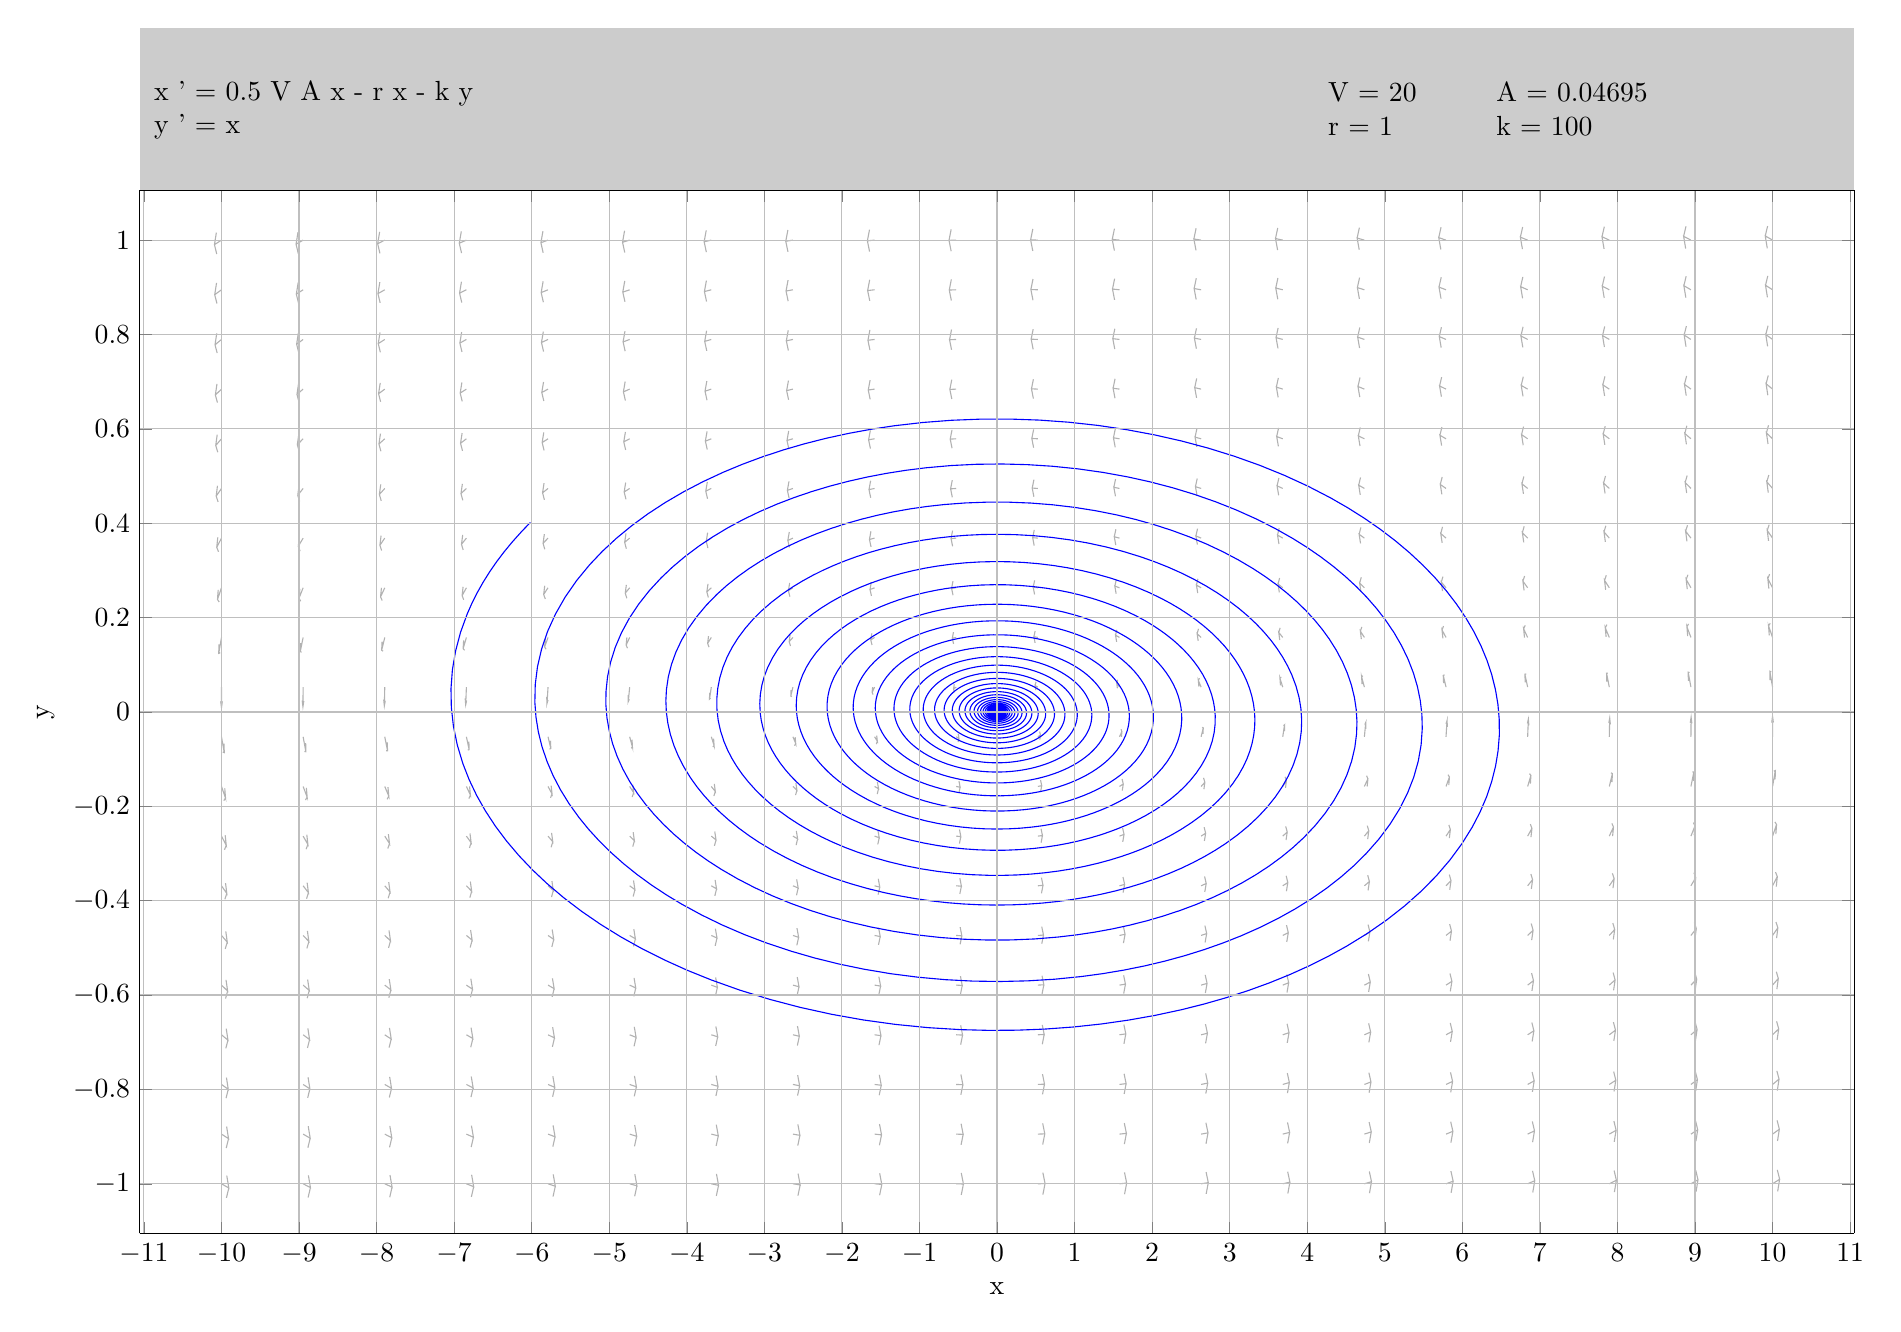
\begin{tikzpicture}

\begin{axis}[%
width=8.571659in,
height=0.813967in,
at={(0.866319in,6.91182in)},
scale only axis,
every outer x axis line/.append style={black},
every x tick label/.append style={font=\color{black}},
xmin=0,
xmax=1,
xtick={-1},
xticklabels={\empty},
every outer y axis line/.append style={black},
every y tick label/.append style={font=\color{black}},
ymin=0,
ymax=1,
ytick={-1},
yticklabels={\empty},
hide axis,
axis background/.style={fill=white!80!black},
axis x line*=bottom,
axis y line*=left
]
\node[right, align=left, inner sep=0mm, text=black]
at (axis cs:0.00806451612903225,0.495614035087719,0) {x ' = 0.5 V A x - r x - k y\\y ' = x};
\node[right, align=left, inner sep=0mm, text=black]
at (axis cs:0.790952380952381,0.5,0) {A = 0.04695\\k = 100};
\node[right, align=left, inner sep=0mm, text=black]
at (axis cs:0.692857142857143,0.5,0) {V = 20\\r = 1};
\node[right, align=left, inner sep=0mm, text=black]
at (axis cs:0.661428571428571,0.5,0) { \\ };
\end{axis}

\begin{axis}[%
width=8.571659in,
height=5.214906in,
at={(0.866319in,1.696914in)},
scale only axis,
unbounded coords=jump,
separate axis lines,
every outer x axis line/.append style={black},
every x tick label/.append style={font=\color{black}},
xmin=-11.0526315789474,
xmax=11.0526315789474,
xlabel={x},
xmajorgrids,
every outer y axis line/.append style={black},
every y tick label/.append style={font=\color{black}},
ymin=-1.10526315789474,
ymax=1.10526315789474,
ylabel={y},
ymajorgrids,
every outer z axis line/.append style={black},
every z tick label/.append style={font=\color{black}},
zmin=-1,
zmax=1,
view={0}{90}
]
\addplot [color=white!70!black,solid,forget plot]
  table[row sep=crcr]{%
-10	-1\\
-9.90568745073129	-1.00895613211801\\
-9.9317421824824	-0.98269115516543\\
-9.90568745073129	-1.00895613211801\\
-9.93622024854141	-1.02984742979978\\
nan	0\\
-10	-0.894736842105263\\
-9.90900440830407	-0.904337691964479\\
-9.93390287334804	-0.878708539082732\\
-9.90900440830407	-0.904337691964479\\
-9.93870329827765	-0.924206334930697\\
nan	0\\
-10	-0.789473684210526\\
-9.91259123428432	-0.799848320241985\\
-9.93622020499116	-0.774883738003628\\
-9.91259123428432	-0.799848320241985\\
-9.94140752300689	-0.818588120861466\\
nan	0\\
-10	-0.684210526315789\\
-9.916512653671	-0.695534521477473\\
-9.93872785877928	-0.671265486346717\\
-9.916512653671	-0.695534521477473\\
-9.94438985636012	-0.713009159511219\\
nan	0\\
-10	-0.578947368421053\\
-9.92086326766601	-0.591469055422963\\
-9.94147386561573	-0.567928366238891\\
-9.92086326766601	-0.591469055422963\\
-9.94773470911668	-0.607496732405888\\
nan	0\\
-10	-0.473684210526316\\
-9.92579086069872	-0.487772746607374\\
-9.94453146846884	-0.464993900957737\\
-9.92579086069872	-0.487772746607374\\
-9.95157573650937	-0.502098470608375\\
nan	0\\
-10	-0.368421052631579\\
-9.93154890962335	-0.384662047107772\\
-9.9480239881173	-0.362676976170752\\
-9.93154890962335	-0.384662047107772\\
-9.9561444853554	-0.396902521359076\\
nan	0\\
-10	-0.263157894736842\\
-9.93863635901856	-0.282564001289782\\
-9.95219392467476	-0.26140125907854\\
-9.93863635901856	-0.282564001289782\\
-9.96189697795123	-0.29208307956926\\
nan	0\\
-10	-0.157894736842105\\
-9.94826766072207	-0.182418856311678\\
-9.95765633263805	-0.162128535651323\\
-9.94826766072207	-0.182418856311678\\
-9.96991839237284	-0.18799470529029\\
nan	0\\
-10	-0.0526315789473685\\
-9.96447876631377	-0.0862431449743322\\
-9.9667322449129	-0.0672793667446849\\
-9.96447876631377	-0.0862431449743322\\
-9.98353802792638	-0.0850399835878012\\
nan	0\\
-10	0.0526315789473684\\
-9.99981942244857	0.00947467986285646\\
-9.98908437094287	0.0224668939760682\\
-9.99981942244857	0.00947467986285646\\
-10.0106628204851	0.0223766052003519\\
nan	0\\
-10	0.157894736842105\\
-10.0353382663378	0.124189405127673\\
-10.0163104535078	0.125466438057564\\
-10.0353382663378	0.124189405127673\\
-10.033163119365	0.143135571226442\\
nan	0\\
-10	0.263157894736842\\
-10.0516386416519	0.238580692763246\\
-10.030002748663	0.233044192942338\\
-10.0516386416519	0.238580692763246\\
-10.0422913496498	0.258863513768311\\
nan	0\\
-10	0.368421052631579\\
-10.0612995895681	0.348983761524292\\
-10.0380503899209	0.339490051464449\\
-10.0612995895681	0.348983761524292\\
-10.0477690354745	0.370139846248507\\
nan	0\\
-10	0.473684210526316\\
-10.0684009171473	0.457422832959875\\
-10.0438152976115	0.445201016942982\\
-10.0684009171473	0.457422832959875\\
-10.0519459863947	0.479401475516633\\
nan	0\\
-10	0.578947368421053\\
-10.0741670796235	0.564844411441787\\
-10.0483912164916	0.550533528629688\\
-10.0741670796235	0.564844411441787\\
-10.0554426949813	0.587617068441445\\
nan	0\\
-10	0.684210526315789\\
-10.0791000791629	0.671678044345698\\
-10.0522369349215	0.655662769146011\\
-10.0791000791629	0.671678044345698\\
-10.0585031759065	0.69521280872744\\
nan	0\\
-10	0.789473684210526\\
-10.0834546036201	0.778141267096646\\
-10.0555851182556	0.760677341325774\\
-10.0834546036201	0.778141267096646\\
-10.0612513268126	0.802404643135845\\
nan	0\\
-10	0.894736842105263\\
-10.0873790113822	0.884355426237614\\
-10.0585699540006	0.865625098152352\\
-10.0873790113822	0.884355426237614\\
-10.0637606619345	0.909314603843466\\
nan	0\\
-10	1\\
-10.0909682121894	0.990393556978788\\
-10.0612761377773	0.970533436837809\\
-10.0909682121894	0.990393556978788\\
-10.0660793592879	1.01601754293249\\
nan	0\\
-8.94736842105263	-1\\
-8.8531692784984	-1.00804641489822\\
-8.87941741754011	-0.982082704790198\\
-8.8531692784984	-1.00804641489822\\
-8.88344062498923	-1.02918227606731\\
nan	0\\
-8.94736842105263	-0.894736842105263\\
-8.8564885035489	-0.903367003778852\\
-8.88159493838162	-0.878057975900843\\
-8.8564885035489	-0.903367003778852\\
-8.88591001921842	-0.923497934652709\\
nan	0\\
-8.94736842105263	-0.789473684210526\\
-8.8600768443481	-0.798805660074825\\
-8.88393132339339	-0.774183173139403\\
-8.8600768443481	-0.798805660074825\\
-8.88859731132554	-0.817828961491667\\
nan	0\\
-8.94736842105263	-0.684210526315789\\
-8.86399831849292	-0.69440551290761\\
-8.88646060261288	-0.670504491290137\\
-8.86399831849292	-0.69440551290761\\
-8.89155809590879	-0.712189542569991\\
nan	0\\
-8.94736842105263	-0.578947368421053\\
-8.86834618478662	-0.590234504593347\\
-8.88923107162335	-0.567092804675155\\
-8.86834618478662	-0.590234504593347\\
-8.89487463970949	-0.606603922808163\\
nan	0\\
-8.94736842105263	-0.473684210526316\\
-8.87326556088808	-0.486406566679937\\
-8.89231582989904	-0.464064144792713\\
-8.87326556088808	-0.486406566679937\\
-8.89867700797585	-0.501115574874988\\
nan	0\\
-8.94736842105263	-0.368421052631579\\
-8.87900436417617	-0.383128861143508\\
-8.89583662911113	-0.361625504370814\\
-8.87900436417617	-0.383128861143508\\
-8.90319053336709	-0.395807532809045\\
nan	0\\
-8.94736842105263	-0.263157894736842\\
-8.88604983441457	-0.280820423822588\\
-8.90002977813455	-0.260192018437348\\
-8.88604983441457	-0.280820423822588\\
-8.90886104267742	-0.29085131175638\\
nan	0\\
-8.94736842105263	-0.157894736842105\\
-8.89560012334637	-0.180449705921042\\
-8.90549187038851	-0.160741140770795\\
-8.89560012334637	-0.180449705921042\\
-8.91676935492798	-0.186625289623927\\
nan	0\\
-8.94736842105263	-0.0526315789473685\\
-8.91187208875351	-0.0843605612059628\\
-8.9145887428786	-0.065967783453604\\
-8.91187208875351	-0.0843605612059628\\
-8.9304532340079	-0.0837159496031651\\
nan	0\\
-8.94736842105263	0.0526315789473684\\
-8.94976676153383	0.0110912955236224\\
-8.93866218853354	0.0229537954304461\\
-8.94976676153383	0.0110912955236224\\
-8.95943233024541	0.0241529656710463\\
nan	0\\
-8.94736842105263	0.157894736842105\\
-8.98506928006451	0.127348083685657\\
-8.96612235907184	0.127086864879621\\
-8.98506928006451	0.127348083685657\\
-8.98139568565006	0.145937294385562\\
nan	0\\
-8.94736842105263	0.263157894736842\\
-9.00025500329586	0.241219412784377\\
-8.97890440813478	0.234579311809308\\
-9.00025500329586	0.241219412784377\\
-8.98987364911101	0.261022602930925\\
nan	0\\
-8.94736842105263	0.368421052631579\\
-9.00946004739266	0.351111579303102\\
-8.98650519115853	0.340781514716638\\
-9.00946004739266	0.351111579303102\\
-8.99515992782277	0.371827327886652\\
nan	0\\
-8.94736842105263	0.473684210526316\\
-9.01634270541325	0.459204819132842\\
-8.9920305722567	0.446305065460728\\
-9.01634270541325	0.459204819132842\\
-8.99927026795344	0.48079220764104\\
nan	0\\
-8.94736842105263	0.578947368421053\\
-9.02198519420891	0.566385808693214\\
-8.99645977233007	0.551500083322496\\
-9.02198519420891	0.566385808693214\\
-9.00274055219399	0.588808469900635\\
nan	0\\
-8.94736842105263	0.684210526315789\\
-9.02683978653176	0.673043420492625\\
-9.00020660043223	0.656525710869793\\
-9.02683978653176	0.673043420492625\\
-9.00579015334381	0.696261393609356\\
nan	0\\
-8.94736842105263	0.789473684210526\\
-9.03114047683792	0.779372181897457\\
-9.00348348452407	0.761459618645054\\
-9.03114047683792	0.779372181897457\\
-9.0085342356806	0.803345646537701\\
nan	0\\
-8.94736842105263	0.894736842105263\\
-9.03502572311196	0.885480038466283\\
-9.00641433158441	0.866342754043146\\
-9.03502572311196	0.885480038466283\\
-9.0110427334039	0.910171405072808\\
nan	0\\
-8.94736842105263	1\\
-9.0385851716263	0.991431805130622\\
-9.00907809773685	0.971198075948019\\
-9.0385851716263	0.991431805130622\\
-9.01336219517154	1.01680645123485\\
nan	0\\
-7.89473684210526	-1\\
-7.80065696581268	-1.00712879352583\\
-7.827098730319	-0.981470186394933\\
-7.80065696581268	-1.00712879352583\\
-7.83066312708191	-1.02851012454122\\
nan	0\\
-7.89473684210526	-0.894736842105263\\
-7.80397942781037	-0.902386765342122\\
-7.82929417128962	-0.877402434797342\\
-7.80397942781037	-0.902386765342122\\
-7.83311913290805	-0.922781141944788\\
nan	0\\
-7.89473684210526	-0.789473684210526\\
-7.80757052369185	-0.7977511941496\\
-7.83165104173111	-0.773476361564524\\
-7.80757052369185	-0.7977511941496\\
-7.83578979670064	-0.817059520771231\\
nan	0\\
-7.89473684210526	-0.684210526315789\\
-7.81149366860865	-0.693261484780891\\
-7.83420388104136	-0.669735403867207\\
-7.81149366860865	-0.693261484780891\\
-7.83872936027391	-0.711356990615514\\
nan	0\\
-7.89473684210526	-0.578947368421053\\
-7.8158409272841	-0.588980123627948\\
-7.83700151292873	-0.566246318360589\\
-7.8158409272841	-0.588980123627948\\
-7.84201789053217	-0.60569427577117\\
nan	0\\
-7.89473684210526	-0.473684210526316\\
-7.82075493428576	-0.485012884872768\\
-7.840117338045	-0.463118805613956\\
-7.82075493428576	-0.485012884872768\\
-7.84578167521822	-0.500109759523709\\
nan	0\\
-7.89473684210526	-0.368421052631579\\
-7.82647812376933	-0.381554885489727\\
-7.84367228105557	-0.360550056048298\\
-7.82647812376933	-0.381554885489727\\
-7.85023919748464	-0.394679415216266\\
nan	0\\
-7.89473684210526	-0.263157894736842\\
-7.83348502513009	-0.279010498017308\\
-7.84789741940253	-0.258941762789375\\
-7.83348502513009	-0.279010498017308\\
-7.85582372104276	-0.289567671276961\\
nan	0\\
-7.89473684210526	-0.157894736842105\\
-7.84294905771168	-0.17836017228711\\
-7.8533690341685	-0.159273595555213\\
-7.84294905771168	-0.17836017228711\\
-7.86360175189101	-0.185167487752005\\
nan	0\\
-7.89473684210526	-0.0526315789473685\\
-7.85923423972591	-0.0822871009125809\\
-7.86247113994841	-0.0645147937281788\\
-7.85923423972591	-0.0822871009125809\\
-7.87729890093102	-0.0822660949178556\\
nan	0\\
-7.89473684210526	0.0526315789473684\\
-7.90013497081738	0.0129880388339239\\
-7.88860464717538	0.0235315686899288\\
-7.90013497081738	0.0129880388339239\\
-7.9084264172321	0.0262306330459858\\
nan	0\\
-7.89473684210526	0.157894736842105\\
-7.9346821082466	0.130711840522722\\
-7.91590280432435	0.128880392883203\\
-7.9346821082466	0.130711840522722\\
-7.92949425248404	0.14885302595387\\
nan	0\\
-7.89473684210526	0.263157894736842\\
-7.94877312153397	0.243878732188691\\
-7.92774244706832	0.23615341109596\\
-7.94877312153397	0.243878732188691\\
-7.9373820283424	0.263171550810314\\
nan	0\\
-7.89473684210526	0.368421052631579\\
-7.9575630513074	0.353231575450098\\
-7.93491781925139	0.342081866304008\\
-7.9575630513074	0.353231575450098\\
-7.94251255784213	0.373494970905076\\
nan	0\\
-7.89473684210526	0.473684210526316\\
-7.96424799862663	0.460975341978667\\
-7.94021743453331	0.44741021341262\\
-7.96424799862663	0.460975341978667\\
-7.94657186880713	0.482165791673303\\
nan	0\\
-7.89473684210526	0.578947368421053\\
-7.96977816138161	0.567916476497146\\
-7.94450804261773	0.552465414255231\\
-7.96977816138161	0.567916476497146\\
-7.95002348857968	0.589986073893405\\
nan	0\\
-7.89473684210526	0.684210526315789\\
-7.97456107359392	0.674399489403813\\
-7.94816104491933	0.657386742605242\\
-7.97456107359392	0.674399489403813\\
-7.95306656337532	0.69729885834957\\
nan	0\\
-7.89473684210526	0.789473684210526\\
-7.97881222985251	0.780595138590668\\
-7.95136997712337	0.762239855339815\\
-7.97881222985251	0.780595138590668\\
-7.9558092499333	0.804277549213437\\
nan	0\\
-7.89473684210526	0.894736842105263\\
-7.98266123030165	0.886597830284625\\
-7.95424916088757	0.86705843678172\\
-7.98266123030165	0.886597830284625\\
-7.95831866679789	0.911020630879912\\
nan	0\\
-7.89473684210526	1\\
-7.98619299722494	0.992464164539626\\
-7.95687219182394	0.971860876397819\\
-7.98619299722494	0.992464164539626\\
-7.96064010955413	1.01758895395766\\
nan	0\\
-6.84210526315789	-1\\
-6.74815070121638	-1.00620330633221\\
-6.77478624321578	-0.980853673947167\\
-6.74815070121638	-1.00620330633221\\
-6.77788789638188	-1.02783095491793\\
nan	0\\
-6.84210526315789	-0.894736842105263\\
-6.75147743165142	-0.901397018024991\\
-6.77700073712343	-0.876742007372454\\
-6.75147743165142	-0.901397018024991\\
-6.78033082508329	-0.922055923125692\\
nan	0\\
-6.84210526315789	-0.789473684210526\\
-6.75507261621714	-0.796684963048677\\
-6.77937959058983	-0.772763417662042\\
-6.75507261621714	-0.796684963048677\\
-6.7829852300089	-0.816279741132421\\
nan	0\\
-6.84210526315789	-0.684210526315789\\
-6.75899919526549	-0.692102465719655\\
-6.78195803078225	-0.668958366925395\\
-6.75899919526549	-0.692102465719655\\
-6.78590400048418	-0.710511400871596\\
nan	0\\
-6.84210526315789	-0.578947368421053\\
-6.76334823313135	-0.587705897464652\\
-6.78478570987841	-0.565389081244935\\
-6.76334823313135	-0.587705897464652\\
-6.78916497440021	-0.604767596258209\\
nan	0\\
-6.84210526315789	-0.473684210526316\\
-6.76826016331413	-0.483591547715677\\
-6.78793685896992	-0.462158071597927\\
-6.76826016331413	-0.483591547715677\\
-6.7928905275646	-0.49908062151981\\
nan	0\\
-6.84210526315789	-0.368421052631579\\
-6.77397224509471	-0.379939512312077\\
-6.79153253559354	-0.359450719892131\\
-6.77397224509471	-0.379939512312077\\
-6.79729176543379	-0.393517228923724\\
nan	0\\
-6.84210526315789	-0.263157894736842\\
-6.78094586001224	-0.277131904401646\\
-6.79580017853974	-0.257649850715791\\
-6.78094586001224	-0.277131904401646\\
-6.80278718337214	-0.288229552288618\\
nan	0\\
-6.84210526315789	-0.157894736842105\\
-6.79032197158219	-0.176139903469946\\
-6.80129566739794	-0.157720530587668\\
-6.79032197158219	-0.176139903469946\\
-6.81041825071186	-0.18361217637552\\
nan	0\\
-6.84210526315789	-0.0526315789473685\\
-6.80656207917971	-0.0799781531915263\\
-6.81038839081213	-0.0628883849237325\\
-6.80656207917971	-0.0799781531915263\\
-6.8240616779342	-0.0806599769128253\\
nan	0\\
-6.84210526315789	0.0526315789473684\\
-6.85101778202662	0.0152986499016179\\
-6.83901079410457	0.0242703988981606\\
-6.85101778202662	0.0152986499016179\\
-6.85767725862744	0.0287266583325255\\
nan	0\\
-6.84210526315789	0.157894736842105\\
-6.88413350790854	0.134246061024227\\
-6.86561286552887	0.13083360258193\\
-6.88413350790854	0.134246061024227\\
-6.87743720343781	0.151847724957251\\
nan	0\\
-6.84210526315789	0.263157894736842\\
-6.89719057662392	0.24654418413194\\
-6.87651155493289	0.237756968946903\\
-6.89719057662392	0.24654418413194\\
-6.88481841023534	0.265299625679918\\
nan	0\\
-6.84210526315789	0.368421052631579\\
-6.90560944125468	0.355338508632304\\
-6.88328755182583	0.343387227307889\\
-6.90560944125468	0.355338508632304\\
-6.88982882382547	0.375139316356283\\
nan	0\\
-6.84210526315789	0.473684210526316\\
-6.91211763820017	0.462732074027257\\
-6.88837589156272	0.448514621216406\\
-6.91211763820017	0.462732074027257\\
-6.89385195981225	0.483520808737543\\
nan	0\\
-6.84210526315789	0.578947368421053\\
-6.91754659512143	0.569435205249813\\
-6.89253615473956	0.553428521210301\\
-6.91754659512143	0.569435205249813\\
-6.89729223632518	0.591149187192068\\
nan	0\\
-6.84210526315789	0.684210526315789\\
-6.92226437747386	0.67574554777247\\
-6.89610039854324	0.658245262756475\\
-6.92226437747386	0.67574554777247\\
-6.9003328878149	0.698324819914457\\
nan	0\\
-6.84210526315789	0.789473684210526\\
-6.92647017957409	0.781809693368858\\
-6.89924470693882	0.763017661517309\\
-6.92647017957409	0.781809693368858\\
-6.90307670235965	0.805200119725409\\
nan	0\\
-6.84210526315789	0.894736842105263\\
-6.93028576863237	0.88770850383436\\
-6.9020745324223	0.867771878947013\\
-6.93028576863237	0.88770850383436\\
-6.90558870155775	0.91186213168425\\
nan	0\\
-6.84210526315789	1\\
-6.93379186865998	0.993490425516022\\
-6.90465849338836	0.972521646485693\\
-6.93379186865998	0.993490425516022\\
-6.90791328063035	1.01836494923674\\
nan	0\\
-5.78947368421053	-1\\
-5.69565067545287	-1.00527000005788\\
-5.7224800780657	-0.980233247851099\\
-5.69565067545287	-1.00527000005788\\
-5.72511507809464	-1.02714475222993\\
nan	0\\
-5.78947368421053	-0.894736842105263\\
-5.69898276925013	-0.900397815370413\\
-5.72471480042196	-0.87607679465077\\
-5.69898276925013	-0.900397815370413\\
-5.72754528705454	-0.921322252130966\\
nan	0\\
-5.78947368421053	-0.789473684210526\\
-5.7025834720997	-0.795607025671356\\
-5.72711720036774	-0.7720444702054\\
-5.7025834720997	-0.795607025671356\\
-5.73018387109815	-0.815489576260814\\
nan	0\\
-5.78947368421053	-0.684210526315789\\
-5.70651540137656	-0.690928513227706\\
-5.72972338949877	-0.668173546445639\\
-5.70651540137656	-0.690928513227706\\
-5.73308238295473	-0.709652687862624\\
nan	0\\
-5.78947368421053	-0.578947368421053\\
-5.71086886399356	-0.586411859206577\\
-5.73258418736227	-0.564521306916678\\
-5.71086886399356	-0.586411859206577\\
-5.73631643275503	-0.603823717025161\\
nan	0\\
-5.78947368421053	-0.473684210526316\\
-5.71578248444755	-0.482142487442414\\
-5.73577527514742	-0.46118220442684\\
-5.71578248444755	-0.482142487442414\\
-5.74000441360547	-0.498027804308329\\
nan	0\\
-5.78947368421053	-0.368421052631579\\
-5.72148892923341	-0.378282295779554\\
-5.73941904493955	-0.358327734090883\\
-5.72148892923341	-0.378282295779554\\
-5.74434966651354	-0.39232011157944\\
nan	0\\
-5.78947368421053	-0.263157894736842\\
-5.72843674667853	-0.275182615798746\\
-5.74374164767266	-0.256315965097176\\
-5.72843674667853	-0.275182615798746\\
-5.74975400820361	-0.286834433863173\\
nan	0\\
-5.78947368421053	-0.157894736842105\\
-5.73772840522271	-0.173778373706835\\
-5.74928107970287	-0.156076962900461\\
-5.73772840522271	-0.173778373706835\\
-5.75722289813523	-0.181949602394371\\
nan	0\\
-5.78947368421053	-0.0526315789473685\\
-5.75385499481212	-0.0773738089610982\\
-5.75835504412821	-0.0610464676073789\\
-5.75385499481212	-0.0773738089610982\\
-5.77072615913508	-0.0788558123065797\\
nan	0\\
-5.78947368421053	0.0526315789473684\\
-5.80249671217905	0.0182328977962719\\
-5.78999013350072	0.0252967451494703\\
-5.80249671217905	0.0182328977962719\\
-5.80718947407627	0.0318082591337313\\
nan	0\\
-5.78947368421053	0.157894736842105\\
-5.83338726048343	0.137904696121135\\
-5.81521567742131	0.132923314269202\\
-5.83338726048343	0.137904696121135\\
-5.8252106977818	0.154880102405651\\
nan	0\\
-5.78947368421053	0.263157894736842\\
-5.84550700453633	0.249201741636867\\
-5.8252079701636	0.239380257485408\\
-5.84550700453633	0.249201741636867\\
-5.83218604671358	0.267396917648311\\
nan	0\\
-5.78947368421053	0.368421052631579\\
-5.85360053205307	0.357427507505099\\
-5.83161409141869	0.344693859082407\\
-5.85360053205307	0.357427507505099\\
-5.83711086398193	0.376757283003679\\
nan	0\\
-5.78947368421053	0.473684210526316\\
-5.85995261209359	0.464472865996096\\
-5.83650609759611	0.449616537384397\\
-5.85995261209359	0.464472865996096\\
-5.84111176986122	0.484856001325927\\
nan	0\\
-5.78947368421053	0.578947368421053\\
-5.86529116576573	0.570940875833778\\
-5.84054429815235	0.55438845322116\\
-5.86529116576573	0.570940875833778\\
-5.84454754444599	0.59229719399876\\
nan	0\\
-5.78947368421053	0.684210526315789\\
-5.86995016065465	0.677080942248803\\
-5.84402482170466	0.659100698357869\\
-5.86995016065465	0.677080942248803\\
-5.84758961373816	0.699338936579929\\
nan	0\\
-5.78947368421053	0.789473684210526\\
-5.87411465571487	0.783015432098891\\
-5.84710780123566	0.763792664856297\\
-5.87411465571487	0.783015432098891\\
-5.85033692729147	0.806113150608467\\
nan	0\\
-5.78947368421053	0.894736842105263\\
-5.87789958083712	0.888811779970072\\
-5.84989054631534	0.868482824453981\\
-5.87789958083712	0.888811779970072\\
-5.85285307738294	0.912695772767278\\
nan	0\\
-5.78947368421053	1\\
-5.8813819697644	0.994510390758845\\
-5.85243708178795	0.973180202142723\\
-5.8813819697644	0.994510390758845\\
-5.85518188640853	1.01913434491966\\
nan	0\\
-4.73684210526316	-1\\
-4.64315708121373	-1.00432893020619\\
-4.67018035587701	-0.979608995131972\\
-4.64315708121373	-1.00432893020619\\
-4.6723448209801	-1.02645150715669\\
nan	0\\
-4.73684210526316	-0.894736842105263\\
-4.64649569800634	-0.89938922369017\\
-4.67243652478716	-0.875406907400493\\
-4.64649569800634	-0.89938922369017\\
-4.67476271557961	-0.920580111028904\\
nan	0\\
-4.73684210526316	-0.789473684210526\\
-4.65010344715354	-0.794517460304047\\
-4.67486410056305	-0.771319662948586\\
-4.65010344715354	-0.794517460304047\\
-4.67738598860981	-0.814688992003395\\
nan	0\\
-4.73684210526316	-0.684210526315789\\
-4.65404280045042	-0.689739715764199\\
-4.67750029453214	-0.667381132726492\\
-4.65404280045042	-0.689739715764199\\
-4.68026488925635	-0.70878078513286\\
nan	0\\
-4.73684210526316	-0.578947368421053\\
-4.65840360336421	-0.585098094558745\\
-4.68039747239947	-0.563643251242699\\
-4.65840360336421	-0.585098094558745\\
-4.68347283546832	-0.602862502192175\\
nan	0\\
-4.73684210526316	-0.473684210526316\\
-4.66332318499919	-0.48066573279629\\
-4.68363348051089	-0.460191546049307\\
-4.66332318499919	-0.48066573279629\\
-4.68712424164588	-0.496951006181289\\
nan	0\\
-4.73684210526316	-0.368421052631579\\
-4.66903051762849	-0.376582983352775\\
-4.68733351123859	-0.357181507227748\\
-4.66903051762849	-0.376582983352775\\
-4.69141447659919	-0.391087301045084\\
nan	0\\
-4.73684210526316	-0.263157894736842\\
-4.67596258741696	-0.273161010431477\\
-4.69172566384716	-0.254940196261537\\
-4.67596258741696	-0.273161010431477\\
-4.69672722169448	-0.285379955184636\\
nan	0\\
-4.73684210526316	-0.157894736842105\\
-4.68518032201721	-0.17126534027892\\
-4.69733620613179	-0.154338713436389\\
-4.68518032201721	-0.17126534027892\\
-4.7040215078502	-0.180169605059361\\
nan	0\\
-4.73684210526316	-0.0526315789473685\\
-4.70111874551426	-0.0743927375476681\\
-4.70639546378885	-0.0589335500303525\\
-4.70111874551426	-0.0743927375476681\\
-4.717276043089	-0.0767952299048039\\
nan	0\\
-4.73684210526316	0.0526315789473684\\
-4.75457224314528	0.0220945507320524\\
-4.74161894472682	0.0268231247261157\\
-4.75457224314528	0.0220945507320524\\
-4.75688745883448	0.0356881936671787\\
nan	0\\
-4.73684210526316	0.157894736842105\\
-4.7824180684447	0.141634061389333\\
-4.76468011062705	0.135118273229778\\
-4.7824180684447	0.141634061389333\\
-4.77281044835343	0.157906254820551\\
nan	0\\
-4.73684210526316	0.263157894736842\\
-4.79372394599214	0.251838250585625\\
-4.77382948273564	0.241013683648744\\
-4.79372394599214	0.251838250585625\\
-4.77948930481125	0.269454604013236\\
nan	0\\
-4.73684210526316	0.368421052631579\\
-4.80153805099484	0.359494122035645\\
-4.77989753462635	0.345998214781505\\
-4.80153805099484	0.359494122035645\\
-4.78436099992432	0.378346187647344\\
nan	0\\
-4.73684210526316	0.473684210526316\\
-4.80775403363709	0.466195755130156\\
-4.78460834127587	0.45071430965552\\
-4.80775403363709	0.466195755130156\\
-4.78835256897395	0.486170273842488\\
nan	0\\
-4.73684210526316	0.578947368421053\\
-4.81301259171371	0.572432461121444\\
-4.78853271895365	0.555344311698687\\
-4.81301259171371	0.572432461121444\\
-4.79179017260345	0.593429554923965\\
nan	0\\
-4.73684210526316	0.684210526315789\\
-4.81761890725869	0.678405069615998\\
-4.79193450248508	0.659952506127053\\
-4.81761890725869	0.678405069615998\\
-4.79483723083498	0.700340907124817\\
nan	0\\
-4.73684210526316	0.789473684210526\\
-4.82174599893253	0.784211970234507\\
-4.79495940233771	0.76456451100997\\
-4.82174599893253	0.784211970234507\\
-4.79759025932572	0.807016457844656\\
nan	0\\
-4.73684210526316	0.894736842105263\\
-4.82550291569255	0.889907398140109\\
-4.79769731157244	0.869191028722308\\
-4.82550291569255	0.889907398140109\\
-4.80011203355502	0.913521433937003\\
nan	0\\
-4.73684210526316	1\\
-4.82896348794376	0.99552387525408\\
-4.8002080419531	0.973836367007704\\
-4.82896348794376	0.99552387525408\\
-4.80244610432606	1.01989705834801\\
nan	0\\
-3.68421052631579	-1\\
-3.59067011286216	-1.00338016139389\\
-3.61788719654978	-0.978981009612316\\
-3.59067011286216	-1.00338016139389\\
-3.61957727724672	-1.02575121633913\\
nan	0\\
-3.68421052631579	-0.894736842105263\\
-3.5940164781049	-0.898371322657876\\
-3.62016607243001	-0.874732466439369\\
-3.5940164781049	-0.898371322657876\\
-3.62198331270632	-0.919829490544814\\
nan	0\\
-3.68421052631579	-0.789473684210526\\
-3.59763290210993	-0.793416365688998\\
-3.62262051900207	-0.770589155193992\\
-3.59763290210993	-0.793416365688998\\
-3.62459185974131	-0.81387796729692\\
nan	0\\
-3.68421052631579	-0.684210526315789\\
-3.60158191533818	-0.688536194829764\\
-3.62528908150297	-0.666581341531168\\
-3.60158191533818	-0.688536194829764\\
-3.62745191575995	-0.707895647019975\\
nan	0\\
-3.68421052631579	-0.578947368421053\\
-3.60595325426413	-0.583764746343301\\
-3.62822609139906	-0.562755214953712\\
-3.60595325426413	-0.583764746343301\\
-3.63063478036019	-0.601883850979542\\
nan	0\\
-3.68421052631579	-0.473684210526316\\
-3.61088359870783	-0.479161420248028\\
-3.63151237455979	-0.459186525429525\\
-3.61088359870783	-0.479161420248028\\
-3.63425097942065	-0.495849989233504\\
nan	0\\
-3.68421052631579	-0.368421052631579\\
-3.61659948413656	-0.374841549491104\\
-3.63527767257545	-0.356012639888439\\
-3.61659948413656	-0.374841549491104\\
-3.63848792100521	-0.389818160978054\\
nan	0\\
-3.68421052631579	-0.263157894736842\\
-3.6235287800207	-0.271066003947109\\
-3.63975627660666	-0.253523134610255\\
-3.6235287800207	-0.271066003947109\\
-3.64371033121179	-0.283864007757802\\
nan	0\\
-3.68421052631579	-0.157894736842105\\
-3.63269248604206	-0.168591528391962\\
-3.64547370023672	-0.152502980858573\\
-3.63269248604206	-0.168591528391962\\
-3.65082209601164	-0.178262000995437\\
nan	0\\
-3.68421052631579	-0.0526315789473685\\
-3.64837362917068	-0.0709243765567166\\
-3.65455149891187	-0.0564773129876337\\
-3.64837362917068	-0.0709243765567166\\
-3.66369789771655	-0.0743957615601905\\
nan	0\\
-3.68421052631579	0.0526315789473684\\
-3.70702426958202	0.0272285402352631\\
-3.69382938692413	0.0291460160323358\\
-3.70702426958202	0.0272285402352631\\
-3.70653090628018	0.0405528876654536\\
nan	0\\
-3.68421052631579	0.157894736842105\\
-3.7312137510015	0.145377947889601\\
-3.71398358635766	0.137382178403924\\
-3.7312137510015	0.145377947889601\\
-3.72024198083392	0.160883790746781\\
nan	0\\
-3.68421052631579	0.263157894736842\\
-3.74184460765643	0.254441777307689\\
-3.72237535389695	0.242648092201273\\
-3.74184460765643	0.254441777307689\\
-3.72673341261153	0.271465132871596\\
nan	0\\
-3.68421052631579	0.368421052631579\\
-3.74942407084401	0.361534359086173\\
-3.72813833409919	0.34729698101774\\
-3.74942407084401	0.361534359086173\\
-3.73158168087189	0.37990375328185\\
nan	0\\
-3.68421052631579	0.473684210526316\\
-3.75552312032281	0.467898969984062\\
-3.73268303198514	0.451806393644983\\
-3.75552312032281	0.467898969984062\\
-3.73557565225627	0.487462690648494\\
nan	0\\
-3.68421052631579	0.578947368421053\\
-3.76071163130459	0.573909026440447\\
-3.7365017143128	0.556295252787428\\
-3.76071163130459	0.573909026440447\\
-3.7390208853031	0.59454580528183\\
nan	0\\
-3.68421052631579	0.684210526315789\\
-3.76527111943753	0.679717376597869\\
-3.73982965407152	0.660800173232811\\
-3.76527111943753	0.679717376597869\\
-3.74207622893048	0.701330469793679\\
nan	0\\
-3.68421052631579	0.789473684210526\\
-3.76936455903393	0.785398952577553\\
-3.74279966631024	0.765332863887911\\
-3.76936455903393	0.785398952577553\\
-3.74483703212673	0.807909880246979\\
nan	0\\
-3.68421052631579	0.894736842105263\\
-3.77309602704402	0.890995116197883\\
-3.7454949453487	0.86989625878804\\
-3.77309602704402	0.890995116197883\\
-3.74736580830239	0.914339009152154\\
nan	0\\
-3.68421052631579	1\\
-3.77653661360967	0.996530706137819\\
-3.74797146395596	0.974489972473002\\
-3.77653661360967	0.996530706137819\\
-3.74970611088705	1.02065301611994\\
nan	0\\
-2.63157894736842	-1\\
-2.53818996613236	-1.00242376769666\\
-2.56560071857902	-0.978349392078646\\
-2.53818996613236	-1.00242376769666\\
-2.56681260242735	-1.02504388269667\\
nan	0\\
-2.63157894736842	-0.894736842105263\\
-2.5415453720344	-0.897344205894783\\
-2.56790360368723	-0.874053602924422\\
-2.5415453720344	-0.897344205894783\\
-2.56920728558199	-0.919070390591432\\
nan	0\\
-2.63157894736842	-0.789473684210526\\
-2.54517220180769	-0.792303862083824\\
-2.57038668100759	-0.769853122331653\\
-2.54517220180769	-0.792303862083824\\
-2.57180176994424	-0.813056495112017\\
nan	0\\
-2.63157894736842	-0.684210526315789\\
-2.54913327678768	-0.687318107046675\\
-2.57309008277918	-0.665774415182223\\
-2.54913327678768	-0.687318107046675\\
-2.57464387314462	-0.706997250472595\\
nan	0\\
-2.63157894736842	-0.578947368421053\\
-2.55351863647024	-0.582412019045681\\
-2.57607056708353	-0.561857546133746\\
-2.55351863647024	-0.582412019045681\\
-2.57780289239585	-0.600887701582839\\
nan	0\\
-2.63157894736842	-0.473684210526316\\
-2.55846509998769	-0.477629805484937\\
-2.57941285546225	-0.458167665152168\\
-2.55846509998769	-0.477629805484937\\
-2.58138565294157	-0.494724588842533\\
nan	0\\
-2.63157894736842	-0.368421052631579\\
-2.56419842242438	-0.373058231320822\\
-2.58325328523528	-0.354821946478038\\
-2.56419842242438	-0.373058231320822\\
-2.5855718745799	-0.38851220895006\\
nan	0\\
-2.63157894736842	-0.263157894736842\\
-2.57114119775284	-0.268897199576648\\
-2.58783769642757	-0.252065970720812\\
-2.57114119775284	-0.268897199576648\\
-2.59070734884747	-0.282284845528601\\
nan	0\\
-2.63157894736842	-0.157894736842105\\
-2.5802827574838	-0.165749600923665\\
-2.59370789842879	-0.150569094228041\\
-2.5802827574838	-0.165749600923665\\
-2.59763533046957	-0.176217189170353\\
nan	0\\
-2.63157894736842	-0.0526315789473685\\
-2.59567130318549	-0.0668215193476579\\
-2.6028961113403	-0.053587626181838\\
-2.59567130318549	-0.0668215193476579\\
-2.60999108154044	-0.0715414482733041\\
nan	0\\
-2.63157894736842	0.0526315789473684\\
-2.65927544800445	0.0337840113148193\\
-2.64625460590551	0.0325141564455763\\
-2.65927544800445	0.0337840113148193\\
-2.65567838972178	0.0463624067635917\\
nan	0\\
-2.63157894736842	0.157894736842105\\
-2.67977529143566	0.149082899550353\\
-2.66311342889255	0.139677364721068\\
-2.67977529143566	0.149082899550353\\
-2.66751934753843	0.163775536754689\\
nan	0\\
-2.63157894736842	0.263157894736842\\
-2.68987356535837	0.257001855031477\\
-2.67084617003505	0.244275012445598\\
-2.68987356535837	0.257001855031477\\
-2.67392418988773	0.273422321440575\\
nan	0\\
-2.63157894736842	0.368421052631579\\
-2.69726094137665	0.36354470280358\\
-2.67633725571718	0.348587109249922\\
-2.69726094137665	0.36354470280358\\
-2.67877543063118	0.381428106254037\\
nan	0\\
-2.63157894736842	0.473684210526316\\
-2.70326117305131	0.469580931916001\\
-2.68073068569386	0.452891359078374\\
-2.70326117305131	0.469580931916001\\
-2.68278232499902	0.488732471919818\\
nan	0\\
-2.63157894736842	0.578947368421053\\
-2.70838907497547	0.575369729090512\\
-2.68445162686072	0.557240488987911\\
-2.70838907497547	0.575369729090512\\
-2.68624044652599	0.595645552791436\\
nan	0\\
-2.63157894736842	0.684210526315789\\
-2.71290731390009	0.681017359330506\\
-2.68771051219427	0.661643217793175\\
-2.71290731390009	0.681017359330506\\
-2.68930709568691	0.702307401059008\\
nan	0\\
-2.63157894736842	0.789473684210526\\
-2.71697069324849	0.786576052900865\\
-2.69062876165706	0.766097405823745\\
-2.71697069324849	0.786576052900865\\
-2.69207757731189	0.808793278763781\\
nan	0\\
-2.63157894736842	0.894736842105263\\
-2.72067917286779	0.892074710149322\\
-2.69328357222899	0.870598293361263\\
-2.72067917286779	0.892074710149322\\
-2.69461463820696	0.915148406110945\\
nan	0\\
-2.63157894736842	1\\
-2.72410153963402	0.997530722527239\\
-2.69572744258615	0.975140857702667\\
-2.72410153963402	0.997530722527239\\
-2.69696208132253	1.02140215383547\\
nan	0\\
-1.57894736842105	-1\\
-1.48571683780412	-1.00145983298764\\
-1.51332103874229	-0.977714250437112\\
-1.48571683780412	-1.00145983298764\\
-1.51405095523611	-1.02432951574558\\
nan	0\\
-1.57894736842105	-0.894736842105263\\
-1.48908264405994	-0.896307981544474\\
-1.51564927650847	-0.873370458622433\\
-1.48908264405994	-0.896307981544474\\
-1.51643484622808	-0.918302820802988\\
nan	0\\
-1.57894736842105	-0.789473684210526\\
-1.49272171429173	-0.791180092303249\\
-1.51816280850735	-0.769111756343102\\
-1.49272171429173	-0.791180092303249\\
-1.51901601255371	-0.812224583407763\\
nan	0\\
-1.57894736842105	-0.684210526315789\\
-1.4966974217961	-0.6860856462124\\
-1.52090362580943	-0.664960623587179\\
-1.4966974217961	-0.6860856462124\\
-1.52184118575774	-0.706085596899655\\
nan	0\\
-1.57894736842105	-0.578947368421053\\
-1.50110058324326	-0.58104018333557\\
-1.52393141506797	-0.560950642566766\\
-1.50110058324326	-0.58104018333557\\
-1.52497782252522	-0.599874035155664\\
nan	0\\
-1.57894736842105	-0.473684210526316\\
-1.50606909671272	-0.47607127499327\\
-1.52733581210848	-0.4571355877261\\
-1.50606909671272	-0.47607127499327\\
-1.52852934434196	-0.493574723580267\\
nan	0\\
-1.57894736842105	-0.368421052631579\\
-1.51183002797592	-0.37123356558822\\
-1.5312621018703	-0.353610476589945\\
-1.51183002797592	-0.37123356558822\\
-1.53266835834862	-0.387169146812511\\
nan	0\\
-1.57894736842105	-0.263157894736842\\
-1.5188061418987	-0.266655053756585\\
-1.53597422010047	-0.250570599420075\\
-1.5188061418987	-0.266655053756585\\
-1.53772279961034	-0.280641212681249\\
nan	0\\
-1.57894736842105	-0.157894736842105\\
-1.52797219617795	-0.162735454020122\\
-1.54205456855637	-0.148539445805941\\
-1.52797219617795	-0.162735454020122\\
-1.54447492714538	-0.174027031927494\\
nan	0\\
-1.57894736842105	-0.0526315789473685\\
-1.54312708855442	-0.061902237585155\\
-1.55155550785496	-0.0501659700271605\\
-1.54312708855442	-0.061902237585155\\
-1.55619083717386	-0.0680761099604775\\
nan	0\\
-1.57894736842105	0.0526315789473684\\
-1.61054797633237	0.041357056293632\\
-1.59824916329554	0.0368392611119245\\
-1.61054797633237	0.041357056293632\\
-1.60388642462241	0.0526395650675814\\
nan	0\\
-1.57894736842105	0.157894736842105\\
-1.62811495344507	0.152702531865706\\
-1.61206662669376	0.141968297102623\\
-1.62811495344507	0.152702531865706\\
-1.61466272918196	0.166552089614629\\
nan	0\\
-1.57894736842105	0.263157894736842\\
-1.63781644033298	0.259509626029161\\
-1.61924365158248	0.245886838663484\\
-1.63781644033298	0.259509626029161\\
-1.62106778593632	0.275321374619447\\
nan	0\\
-1.57894736842105	0.368421052631579\\
-1.64505122221396	0.365522121045903\\
-1.62449533317967	0.349865837073378\\
-1.64505122221396	0.365522121045903\\
-1.62594479897251	0.382917763969833\\
nan	0\\
-1.57894736842105	0.473684210526316\\
-1.65096955624345	0.471240253627746\\
-1.62875191067209	0.453967893741717\\
-1.65096955624345	0.471240253627746\\
-1.62997388912137	0.489978987652917\\
nan	0\\
-1.57894736842105	0.578947368421053\\
-1.65604573778715	0.576813817010432\\
-1.63238283912467	0.558179290092094\\
-1.65604573778715	0.576813817010432\\
-1.63344961482998	0.596728474775142\\
nan	0\\
-1.57894736842105	0.684210526315789\\
-1.66052801860382	0.682304562531863\\
-1.63557733260301	0.66248118912135\\
-1.66052801860382	0.682304562531863\\
-1.63653031449497	0.703271514212732\\
nan	0\\
-1.57894736842105	0.789473684210526\\
-1.66456476457973	0.787742973446142\\
-1.63844686804103	0.766857837635788\\
-1.66456476457973	0.787742973446142\\
-1.63931222342322	0.809666535715127\\
nan	0\\
-1.57894736842105	0.894736842105263\\
-1.66825261437341	0.893145973842337\\
-1.64106332352197	0.871296922833126\\
-1.66825261437341	0.893145973842337\\
-1.64185875765343	0.915949545809303\\
nan	0\\
-1.57894736842105	1\\
-1.67165846082534	0.99852377532217\\
-1.64347607693459	0.975788869624448\\
-1.67165846082534	0.99852377532217\\
-1.64421418927351	1.02214441582659\\
nan	0\\
-0.526315789473685	-1\\
-0.433250925352403	-1.00048845126697\\
-0.461048271772046	-0.977075699856558\\
-0.433250925352403	-1.00048845126697\\
-0.46129249740553	-1.0236081319172\\
nan	0\\
-0.526315789473685	-0.894736842105263\\
-0.436628559649206	-0.895262772832168\\
-0.463403245914824	-0.872683186157977\\
-0.436628559649206	-0.895262772832168\\
-0.463666211278276	-0.917526801070216\\
nan	0\\
-0.526315789473685	-0.789473684210526\\
-0.440281809817367	-0.790045222733658\\
-0.465949119083479	-0.768365266262639\\
-0.440281809817367	-0.790045222733658\\
-0.466234888345045	-0.811382256090798\\
nan	0\\
-0.526315789473685	-0.684210526315789\\
-0.44427489175346	-0.684839045303461\\
-0.468730031322609	-0.664140265177103\\
-0.44427489175346	-0.684839045303461\\
-0.469044290816445	-0.705160714037216\\
nan	0\\
-0.526315789473685	-0.578947368421053\\
-0.448699937528756	-0.579649580497764\\
-0.471809140093057	-0.560034953888518\\
-0.448699937528756	-0.579649580497764\\
-0.472160246131413	-0.598842879860983\\
nan	0\\
-0.526315789473685	-0.473684210526316\\
-0.453697021421734	-0.474486357516026\\
-0.475282115089892	-0.456091021406125\\
-0.453697021421734	-0.474486357516026\\
-0.475683188584747	-0.492400405432101\\
nan	0\\
-0.526315789473685	-0.368421052631579\\
-0.459497074021505	-0.36936842597293\\
-0.479305845321821	-0.35237953510748\\
-0.459497074021505	-0.36936842597293\\
-0.479779531992497	-0.38578889283357\\
nan	0\\
-0.526315789473685	-0.263157894736842\\
-0.466530260044861	-0.264341052026575\\
-0.484170129551075	-0.249039722482449\\
-0.466530260044861	-0.264341052026575\\
-0.484761708195941	-0.278932487196861\\
nan	0\\
-0.526315789473685	-0.157894736842105\\
-0.475784818129523	-0.15954983490287\\
-0.49053033501758	-0.1464205626486\\
-0.475784818129523	-0.15954983490287\\
-0.491357884047962	-0.171686048320681\\
nan	0\\
-0.526315789473685	-0.0526315789473685\\
-0.490971579086962	-0.0559879447786892\\
-0.500735750745149	-0.0461449824326122\\
-0.490971579086962	-0.0559879447786892\\
-0.502413933660809	-0.0638170876259738\\
nan	0\\
-0.526315789473685	0.0526315789473684\\
-0.560406688882678	0.0490315050882424\\
-0.549279400595198	0.041588802393732\\
-0.560406688882678	0.0490315050882424\\
-0.551079437524761	0.0586342520982284\\
nan	0\\
-0.526315789473685	0.157894736842105\\
-0.576253185403744	0.156200191772455\\
-0.560848330357314	0.144224206310835\\
-0.576253185403744	0.156200191772455\\
-0.561695602892139	0.169192904275865\\
nan	0\\
-0.526315789473685	0.263157894736842\\
-0.585679576380848	0.261957886915717\\
-0.567570438353418	0.247476942535263\\
-0.585679576380848	0.261957886915717\\
-0.568170442263981	0.277158835988845\\
nan	0\\
-0.526315789473685	0.368421052631579\\
-0.592797619194604	0.367464059566695\\
-0.572613822012108	0.351130700055931\\
-0.592797619194604	0.367464059566695\\
-0.573092318544549	0.38437161491639\\
nan	0\\
-0.526315789473685	0.473684210526316\\
-0.598649679146077	0.472875735127745\\
-0.576747393394716	0.455034805329219\\
-0.598649679146077	0.472875735127745\\
-0.577151631094002	0.491201750165414\\
nan	0\\
-0.526315789473685	0.578947368421053\\
-0.603682452388288	0.578240626699252\\
-0.580295768083457	0.559110983487142\\
-0.603682452388288	0.578240626699252\\
-0.580649138944357	0.597794314944443\\
nan	0\\
-0.526315789473685	0.684210526315789\\
-0.608133769628331	0.683578578404083\\
-0.583430388604011	0.663313667738934\\
-0.608133769628331	0.683578578404083\\
-0.583746362559864	0.704222657816257\\
nan	0\\
-0.526315789473685	0.789473684210526\\
-0.612147140241273	0.788899444310295\\
-0.586254175035939	0.767613878588467\\
-0.612147140241273	0.788899444310295\\
-0.586541294986054	0.810529553972261\\
nan	0\\
-0.526315789473685	0.894736842105263\\
-0.615816615148923	0.89420871860413\\
-0.588834336571068	0.871991949235661\\
-0.615816615148923	0.89420871860413\\
-0.589098398321635	0.91674236207328\\
nan	0\\
-0.526315789473685	1\\
-0.619207573428338	0.999509726980043\\
-0.591217469986953	0.976433862897367\\
-0.619207573428338	0.999509726980043\\
-0.591462606496931	1.02287975487469\\
nan	0\\
0.526315789473683	-1\\
0.619207573428336	-0.999509726980043\\
0.591217469986951	-0.976433862897367\\
0.619207573428336	-0.999509726980043\\
0.59146260649693	-1.02287975487469\\
nan	0\\
0.526315789473683	-0.894736842105263\\
0.615816615148921	-0.89420871860413\\
0.588834336571066	-0.871991949235661\\
0.615816615148921	-0.89420871860413\\
0.589098398321633	-0.91674236207328\\
nan	0\\
0.526315789473683	-0.789473684210526\\
0.612147140241271	-0.788899444310295\\
0.586254175035937	-0.767613878588468\\
0.612147140241271	-0.788899444310295\\
0.586541294986053	-0.810529553972262\\
nan	0\\
0.526315789473683	-0.684210526315789\\
0.608133769628329	-0.683578578404083\\
0.583430388604009	-0.663313667738934\\
0.608133769628329	-0.683578578404083\\
0.583746362559862	-0.704222657816257\\
nan	0\\
0.526315789473683	-0.578947368421053\\
0.603682452388286	-0.578240626699252\\
0.580295768083455	-0.559110983487142\\
0.603682452388286	-0.578240626699252\\
0.580649138944355	-0.597794314944443\\
nan	0\\
0.526315789473683	-0.473684210526316\\
0.598649679146075	-0.472875735127745\\
0.576747393394715	-0.455034805329219\\
0.598649679146075	-0.472875735127745\\
0.577151631094	-0.491201750165414\\
nan	0\\
0.526315789473683	-0.368421052631579\\
0.592797619194602	-0.367464059566696\\
0.572613822012106	-0.351130700055931\\
0.592797619194602	-0.367464059566696\\
0.573092318544547	-0.38437161491639\\
nan	0\\
0.526315789473683	-0.263157894736842\\
0.585679576380846	-0.261957886915717\\
0.567570438353416	-0.247476942535264\\
0.585679576380846	-0.261957886915717\\
0.568170442263979	-0.277158835988845\\
nan	0\\
0.526315789473683	-0.157894736842105\\
0.576253185403742	-0.156200191772455\\
0.560848330357312	-0.144224206310835\\
0.576253185403742	-0.156200191772455\\
0.561695602892137	-0.169192904275865\\
nan	0\\
0.526315789473683	-0.0526315789473685\\
0.560406688882676	-0.0490315050882426\\
0.549279400595197	-0.0415888023937321\\
0.560406688882676	-0.0490315050882426\\
0.55107943752476	-0.0586342520982286\\
nan	0\\
0.526315789473683	0.0526315789473684\\
0.49097157908696	0.0559879447786891\\
0.500735750745147	0.0461449824326121\\
0.49097157908696	0.0559879447786891\\
0.502413933660807	0.0638170876259736\\
nan	0\\
0.526315789473683	0.157894736842105\\
0.475784818129521	0.15954983490287\\
0.490530335017579	0.1464205626486\\
0.475784818129521	0.15954983490287\\
0.491357884047961	0.171686048320681\\
nan	0\\
0.526315789473683	0.263157894736842\\
0.466530260044859	0.264341052026574\\
0.484170129551073	0.249039722482449\\
0.466530260044859	0.264341052026574\\
0.484761708195939	0.278932487196861\\
nan	0\\
0.526315789473683	0.368421052631579\\
0.459497074021503	0.36936842597293\\
0.479305845321819	0.35237953510748\\
0.459497074021503	0.36936842597293\\
0.479779531992495	0.38578889283357\\
nan	0\\
0.526315789473683	0.473684210526316\\
0.453697021421732	0.474486357516026\\
0.47528211508989	0.456091021406125\\
0.453697021421732	0.474486357516026\\
0.475683188584745	0.492400405432101\\
nan	0\\
0.526315789473683	0.578947368421053\\
0.448699937528755	0.579649580497764\\
0.471809140093055	0.560034953888518\\
0.448699937528755	0.579649580497764\\
0.472160246131411	0.598842879860983\\
nan	0\\
0.526315789473683	0.684210526315789\\
0.444274891753458	0.684839045303461\\
0.468730031322608	0.664140265177103\\
0.444274891753458	0.684839045303461\\
0.469044290816443	0.705160714037216\\
nan	0\\
0.526315789473683	0.789473684210526\\
0.440281809817365	0.790045222733658\\
0.465949119083477	0.768365266262639\\
0.440281809817365	0.790045222733658\\
0.466234888345043	0.811382256090798\\
nan	0\\
0.526315789473683	0.894736842105263\\
0.436628559649204	0.895262772832168\\
0.463403245914822	0.872683186157977\\
0.436628559649204	0.895262772832168\\
0.463666211278274	0.917526801070216\\
nan	0\\
0.526315789473683	1\\
0.433250925352402	1.00048845126697\\
0.461048271772044	0.977075699856558\\
0.433250925352402	1.00048845126697\\
0.461292497405528	1.0236081319172\\
nan	0\\
1.57894736842105	-1\\
1.67165846082534	-0.99852377532217\\
1.64347607693459	-0.975788869624448\\
1.67165846082534	-0.99852377532217\\
1.64421418927351	-1.02214441582659\\
nan	0\\
1.57894736842105	-0.894736842105263\\
1.66825261437341	-0.893145973842337\\
1.64106332352197	-0.871296922833126\\
1.66825261437341	-0.893145973842337\\
1.64185875765343	-0.915949545809303\\
nan	0\\
1.57894736842105	-0.789473684210526\\
1.66456476457973	-0.787742973446143\\
1.63844686804103	-0.766857837635789\\
1.66456476457973	-0.787742973446143\\
1.63931222342322	-0.809666535715127\\
nan	0\\
1.57894736842105	-0.684210526315789\\
1.66052801860382	-0.682304562531863\\
1.63557733260301	-0.66248118912135\\
1.66052801860382	-0.682304562531863\\
1.63653031449497	-0.703271514212732\\
nan	0\\
1.57894736842105	-0.578947368421053\\
1.65604573778715	-0.576813817010432\\
1.63238283912466	-0.558179290092094\\
1.65604573778715	-0.576813817010432\\
1.63344961482997	-0.596728474775142\\
nan	0\\
1.57894736842105	-0.473684210526316\\
1.65096955624345	-0.471240253627746\\
1.62875191067209	-0.453967893741717\\
1.65096955624345	-0.471240253627746\\
1.62997388912137	-0.489978987652917\\
nan	0\\
1.57894736842105	-0.368421052631579\\
1.64505122221396	-0.365522121045903\\
1.62449533317967	-0.349865837073378\\
1.64505122221396	-0.365522121045903\\
1.62594479897251	-0.382917763969833\\
nan	0\\
1.57894736842105	-0.263157894736842\\
1.63781644033298	-0.259509626029161\\
1.61924365158248	-0.245886838663484\\
1.63781644033298	-0.259509626029161\\
1.62106778593632	-0.275321374619447\\
nan	0\\
1.57894736842105	-0.157894736842105\\
1.62811495344506	-0.152702531865706\\
1.61206662669376	-0.141968297102623\\
1.62811495344506	-0.152702531865706\\
1.61466272918196	-0.166552089614629\\
nan	0\\
1.57894736842105	-0.0526315789473685\\
1.61054797633237	-0.0413570562936322\\
1.59824916329554	-0.0368392611119246\\
1.61054797633237	-0.0413570562936322\\
1.60388642462241	-0.0526395650675816\\
nan	0\\
1.57894736842105	0.0526315789473684\\
1.54312708855442	0.0619022375851549\\
1.55155550785496	0.0501659700271604\\
1.54312708855442	0.0619022375851549\\
1.55619083717385	0.0680761099604774\\
nan	0\\
1.57894736842105	0.157894736842105\\
1.52797219617795	0.162735454020122\\
1.54205456855637	0.148539445805941\\
1.52797219617795	0.162735454020122\\
1.54447492714538	0.174027031927494\\
nan	0\\
1.57894736842105	0.263157894736842\\
1.5188061418987	0.266655053756585\\
1.53597422010047	0.250570599420075\\
1.5188061418987	0.266655053756585\\
1.53772279961034	0.280641212681249\\
nan	0\\
1.57894736842105	0.368421052631579\\
1.51183002797592	0.37123356558822\\
1.5312621018703	0.353610476589945\\
1.51183002797592	0.37123356558822\\
1.53266835834862	0.387169146812511\\
nan	0\\
1.57894736842105	0.473684210526316\\
1.50606909671272	0.47607127499327\\
1.52733581210848	0.4571355877261\\
1.50606909671272	0.47607127499327\\
1.52852934434196	0.493574723580267\\
nan	0\\
1.57894736842105	0.578947368421053\\
1.50110058324325	0.58104018333557\\
1.52393141506796	0.560950642566766\\
1.50110058324325	0.58104018333557\\
1.52497782252522	0.599874035155664\\
nan	0\\
1.57894736842105	0.684210526315789\\
1.4966974217961	0.6860856462124\\
1.52090362580943	0.664960623587179\\
1.4966974217961	0.6860856462124\\
1.52184118575774	0.706085596899655\\
nan	0\\
1.57894736842105	0.789473684210526\\
1.49272171429173	0.791180092303249\\
1.51816280850735	0.769111756343101\\
1.49272171429173	0.791180092303249\\
1.51901601255371	0.812224583407763\\
nan	0\\
1.57894736842105	0.894736842105263\\
1.48908264405994	0.896307981544474\\
1.51564927650847	0.873370458622433\\
1.48908264405994	0.896307981544474\\
1.51643484622808	0.918302820802988\\
nan	0\\
1.57894736842105	1\\
1.48571683780412	1.00145983298764\\
1.51332103874229	0.977714250437112\\
1.48571683780412	1.00145983298764\\
1.51405095523611	1.02432951574558\\
nan	0\\
2.63157894736842	-1\\
2.72410153963402	-0.997530722527239\\
2.69572744258615	-0.975140857702667\\
2.72410153963402	-0.997530722527239\\
2.69696208132253	-1.02140215383547\\
nan	0\\
2.63157894736842	-0.894736842105263\\
2.72067917286779	-0.892074710149322\\
2.69328357222899	-0.870598293361264\\
2.72067917286779	-0.892074710149322\\
2.69461463820696	-0.915148406110946\\
nan	0\\
2.63157894736842	-0.789473684210526\\
2.71697069324849	-0.786576052900865\\
2.69062876165706	-0.766097405823745\\
2.71697069324849	-0.786576052900865\\
2.69207757731189	-0.808793278763781\\
nan	0\\
2.63157894736842	-0.684210526315789\\
2.71290731390009	-0.681017359330506\\
2.68771051219427	-0.661643217793175\\
2.71290731390009	-0.681017359330506\\
2.68930709568691	-0.702307401059008\\
nan	0\\
2.63157894736842	-0.578947368421053\\
2.70838907497547	-0.575369729090512\\
2.68445162686072	-0.557240488987911\\
2.70838907497547	-0.575369729090512\\
2.68624044652599	-0.595645552791436\\
nan	0\\
2.63157894736842	-0.473684210526316\\
2.70326117305131	-0.469580931916001\\
2.68073068569386	-0.452891359078374\\
2.70326117305131	-0.469580931916001\\
2.68278232499902	-0.488732471919818\\
nan	0\\
2.63157894736842	-0.368421052631579\\
2.69726094137665	-0.36354470280358\\
2.67633725571718	-0.348587109249922\\
2.69726094137665	-0.36354470280358\\
2.67877543063118	-0.381428106254037\\
nan	0\\
2.63157894736842	-0.263157894736842\\
2.68987356535837	-0.257001855031477\\
2.67084617003505	-0.244275012445599\\
2.68987356535837	-0.257001855031477\\
2.67392418988773	-0.273422321440575\\
nan	0\\
2.63157894736842	-0.157894736842105\\
2.67977529143566	-0.149082899550353\\
2.66311342889255	-0.139677364721068\\
2.67977529143566	-0.149082899550353\\
2.66751934753843	-0.163775536754689\\
nan	0\\
2.63157894736842	-0.0526315789473685\\
2.65927544800445	-0.0337840113148194\\
2.64625460590551	-0.0325141564455764\\
2.65927544800445	-0.0337840113148194\\
2.65567838972178	-0.0463624067635919\\
nan	0\\
2.63157894736842	0.0526315789473684\\
2.59567130318549	0.0668215193476578\\
2.6028961113403	0.0535876261818379\\
2.59567130318549	0.0668215193476578\\
2.60999108154044	0.071541448273304\\
nan	0\\
2.63157894736842	0.157894736842105\\
2.5802827574838	0.165749600923665\\
2.59370789842879	0.150569094228041\\
2.5802827574838	0.165749600923665\\
2.59763533046957	0.176217189170353\\
nan	0\\
2.63157894736842	0.263157894736842\\
2.57114119775284	0.268897199576648\\
2.58783769642757	0.252065970720812\\
2.57114119775284	0.268897199576648\\
2.59070734884747	0.282284845528601\\
nan	0\\
2.63157894736842	0.368421052631579\\
2.56419842242438	0.373058231320822\\
2.58325328523528	0.354821946478038\\
2.56419842242438	0.373058231320822\\
2.5855718745799	0.388512208950059\\
nan	0\\
2.63157894736842	0.473684210526316\\
2.55846509998769	0.477629805484937\\
2.57941285546225	0.458167665152168\\
2.55846509998769	0.477629805484937\\
2.58138565294157	0.494724588842533\\
nan	0\\
2.63157894736842	0.578947368421053\\
2.55351863647024	0.582412019045681\\
2.57607056708353	0.561857546133746\\
2.55351863647024	0.582412019045681\\
2.57780289239585	0.600887701582839\\
nan	0\\
2.63157894736842	0.684210526315789\\
2.54913327678768	0.687318107046674\\
2.57309008277918	0.665774415182223\\
2.54913327678768	0.687318107046674\\
2.57464387314462	0.706997250472595\\
nan	0\\
2.63157894736842	0.789473684210526\\
2.54517220180769	0.792303862083824\\
2.57038668100759	0.769853122331653\\
2.54517220180769	0.792303862083824\\
2.57180176994424	0.813056495112016\\
nan	0\\
2.63157894736842	0.894736842105263\\
2.5415453720344	0.897344205894783\\
2.56790360368723	0.874053602924422\\
2.5415453720344	0.897344205894783\\
2.56920728558199	0.919070390591432\\
nan	0\\
2.63157894736842	1\\
2.53818996613236	1.00242376769666\\
2.56560071857902	0.978349392078646\\
2.53818996613236	1.00242376769666\\
2.56681260242735	1.02504388269667\\
nan	0\\
3.68421052631579	-1\\
3.77653661360967	-0.996530706137819\\
3.74797146395596	-0.974489972473002\\
3.77653661360967	-0.996530706137819\\
3.74970611088705	-1.02065301611994\\
nan	0\\
3.68421052631579	-0.894736842105263\\
3.77309602704402	-0.890995116197883\\
3.7454949453487	-0.86989625878804\\
3.77309602704402	-0.890995116197883\\
3.74736580830239	-0.914339009152154\\
nan	0\\
3.68421052631579	-0.789473684210526\\
3.76936455903393	-0.785398952577553\\
3.74279966631024	-0.765332863887911\\
3.76936455903393	-0.785398952577553\\
3.74483703212673	-0.807909880246979\\
nan	0\\
3.68421052631579	-0.684210526315789\\
3.76527111943753	-0.679717376597869\\
3.73982965407152	-0.660800173232811\\
3.76527111943753	-0.679717376597869\\
3.74207622893048	-0.701330469793679\\
nan	0\\
3.68421052631579	-0.578947368421053\\
3.76071163130459	-0.573909026440447\\
3.7365017143128	-0.556295252787428\\
3.76071163130459	-0.573909026440447\\
3.7390208853031	-0.59454580528183\\
nan	0\\
3.68421052631579	-0.473684210526316\\
3.75552312032281	-0.467898969984062\\
3.73268303198514	-0.451806393644983\\
3.75552312032281	-0.467898969984062\\
3.73557565225627	-0.487462690648494\\
nan	0\\
3.68421052631579	-0.368421052631579\\
3.74942407084401	-0.361534359086173\\
3.72813833409919	-0.34729698101774\\
3.74942407084401	-0.361534359086173\\
3.73158168087189	-0.37990375328185\\
nan	0\\
3.68421052631579	-0.263157894736842\\
3.74184460765643	-0.254441777307689\\
3.72237535389695	-0.242648092201274\\
3.74184460765643	-0.254441777307689\\
3.72673341261153	-0.271465132871596\\
nan	0\\
3.68421052631579	-0.157894736842105\\
3.7312137510015	-0.145377947889601\\
3.71398358635766	-0.137382178403924\\
3.7312137510015	-0.145377947889601\\
3.72024198083392	-0.160883790746781\\
nan	0\\
3.68421052631579	-0.0526315789473685\\
3.70702426958203	-0.0272285402352632\\
3.69382938692413	-0.0291460160323359\\
3.70702426958203	-0.0272285402352632\\
3.70653090628018	-0.0405528876654537\\
nan	0\\
3.68421052631579	0.0526315789473684\\
3.64837362917068	0.0709243765567165\\
3.65455149891187	0.0564773129876336\\
3.64837362917068	0.0709243765567165\\
3.66369789771655	0.0743957615601904\\
nan	0\\
3.68421052631579	0.157894736842105\\
3.63269248604206	0.168591528391962\\
3.64547370023672	0.152502980858573\\
3.63269248604206	0.168591528391962\\
3.65082209601164	0.178262000995437\\
nan	0\\
3.68421052631579	0.263157894736842\\
3.6235287800207	0.271066003947109\\
3.63975627660666	0.253523134610255\\
3.6235287800207	0.271066003947109\\
3.64371033121179	0.283864007757802\\
nan	0\\
3.68421052631579	0.368421052631579\\
3.61659948413656	0.374841549491104\\
3.63527767257545	0.356012639888439\\
3.61659948413656	0.374841549491104\\
3.63848792100521	0.389818160978054\\
nan	0\\
3.68421052631579	0.473684210526316\\
3.61088359870783	0.479161420248028\\
3.63151237455979	0.459186525429525\\
3.61088359870783	0.479161420248028\\
3.63425097942065	0.495849989233503\\
nan	0\\
3.68421052631579	0.578947368421053\\
3.60595325426413	0.583764746343301\\
3.62822609139906	0.562755214953712\\
3.60595325426413	0.583764746343301\\
3.63063478036019	0.601883850979542\\
nan	0\\
3.68421052631579	0.684210526315789\\
3.60158191533818	0.688536194829764\\
3.62528908150297	0.666581341531168\\
3.60158191533818	0.688536194829764\\
3.62745191575995	0.707895647019975\\
nan	0\\
3.68421052631579	0.789473684210526\\
3.59763290210993	0.793416365688997\\
3.62262051900207	0.770589155193992\\
3.59763290210993	0.793416365688997\\
3.62459185974131	0.81387796729692\\
nan	0\\
3.68421052631579	0.894736842105263\\
3.5940164781049	0.898371322657875\\
3.62016607243001	0.874732466439369\\
3.5940164781049	0.898371322657875\\
3.62198331270632	0.919829490544814\\
nan	0\\
3.68421052631579	1\\
3.59067011286216	1.00338016139389\\
3.61788719654978	0.978981009612316\\
3.59067011286216	1.00338016139389\\
3.61957727724672	1.02575121633913\\
nan	0\\
4.73684210526316	-1\\
4.82896348794376	-0.99552387525408\\
4.8002080419531	-0.973836367007704\\
4.82896348794376	-0.99552387525408\\
4.80244610432606	-1.01989705834801\\
nan	0\\
4.73684210526316	-0.894736842105263\\
4.82550291569255	-0.889907398140109\\
4.79769731157244	-0.869191028722308\\
4.82550291569255	-0.889907398140109\\
4.80011203355502	-0.913521433937003\\
nan	0\\
4.73684210526316	-0.789473684210526\\
4.82174599893253	-0.784211970234507\\
4.79495940233771	-0.76456451100997\\
4.82174599893253	-0.784211970234507\\
4.79759025932572	-0.807016457844656\\
nan	0\\
4.73684210526316	-0.684210526315789\\
4.81761890725869	-0.678405069615998\\
4.79193450248508	-0.659952506127053\\
4.81761890725869	-0.678405069615998\\
4.79483723083498	-0.700340907124817\\
nan	0\\
4.73684210526316	-0.578947368421053\\
4.81301259171371	-0.572432461121444\\
4.78853271895364	-0.555344311698687\\
4.81301259171371	-0.572432461121444\\
4.79179017260345	-0.593429554923965\\
nan	0\\
4.73684210526316	-0.473684210526316\\
4.80775403363709	-0.466195755130156\\
4.78460834127587	-0.45071430965552\\
4.80775403363709	-0.466195755130156\\
4.78835256897395	-0.486170273842488\\
nan	0\\
4.73684210526316	-0.368421052631579\\
4.80153805099484	-0.359494122035645\\
4.77989753462635	-0.345998214781505\\
4.80153805099484	-0.359494122035645\\
4.78436099992432	-0.378346187647345\\
nan	0\\
4.73684210526316	-0.263157894736842\\
4.79372394599214	-0.251838250585625\\
4.77382948273564	-0.241013683648744\\
4.79372394599214	-0.251838250585625\\
4.77948930481125	-0.269454604013236\\
nan	0\\
4.73684210526316	-0.157894736842105\\
4.7824180684447	-0.141634061389333\\
4.76468011062705	-0.135118273229778\\
4.7824180684447	-0.141634061389333\\
4.77281044835343	-0.157906254820551\\
nan	0\\
4.73684210526316	-0.0526315789473685\\
4.75457224314528	-0.0220945507320525\\
4.74161894472682	-0.0268231247261158\\
4.75457224314528	-0.0220945507320525\\
4.75688745883447	-0.0356881936671788\\
nan	0\\
4.73684210526316	0.0526315789473684\\
4.70111874551425	0.074392737547668\\
4.70639546378885	0.0589335500303524\\
4.70111874551425	0.074392737547668\\
4.717276043089	0.0767952299048038\\
nan	0\\
4.73684210526316	0.157894736842105\\
4.68518032201721	0.17126534027892\\
4.69733620613179	0.154338713436389\\
4.68518032201721	0.17126534027892\\
4.7040215078502	0.180169605059361\\
nan	0\\
4.73684210526316	0.263157894736842\\
4.67596258741696	0.273161010431477\\
4.69172566384716	0.254940196261537\\
4.67596258741696	0.273161010431477\\
4.69672722169448	0.285379955184636\\
nan	0\\
4.73684210526316	0.368421052631579\\
4.66903051762848	0.376582983352775\\
4.68733351123859	0.357181507227748\\
4.66903051762848	0.376582983352775\\
4.69141447659919	0.391087301045084\\
nan	0\\
4.73684210526316	0.473684210526316\\
4.66332318499919	0.48066573279629\\
4.68363348051089	0.460191546049306\\
4.66332318499919	0.48066573279629\\
4.68712424164587	0.496951006181289\\
nan	0\\
4.73684210526316	0.578947368421053\\
4.65840360336421	0.585098094558745\\
4.68039747239947	0.563643251242699\\
4.65840360336421	0.585098094558745\\
4.68347283546831	0.602862502192175\\
nan	0\\
4.73684210526316	0.684210526315789\\
4.65404280045042	0.689739715764199\\
4.67750029453214	0.667381132726492\\
4.65404280045042	0.689739715764199\\
4.68026488925634	0.70878078513286\\
nan	0\\
4.73684210526316	0.789473684210526\\
4.65010344715354	0.794517460304046\\
4.67486410056305	0.771319662948586\\
4.65010344715354	0.794517460304046\\
4.67738598860981	0.814688992003395\\
nan	0\\
4.73684210526316	0.894736842105263\\
4.64649569800634	0.89938922369017\\
4.67243652478716	0.875406907400493\\
4.64649569800634	0.89938922369017\\
4.67476271557961	0.920580111028903\\
nan	0\\
4.73684210526316	1\\
4.64315708121373	1.00432893020619\\
4.67018035587701	0.979608995131972\\
4.64315708121373	1.00432893020619\\
4.6723448209801	1.02645150715669\\
nan	0\\
5.78947368421053	-1\\
5.8813819697644	-0.994510390758845\\
5.85243708178795	-0.973180202142723\\
5.8813819697644	-0.994510390758845\\
5.85518188640853	-1.01913434491966\\
nan	0\\
5.78947368421053	-0.894736842105263\\
5.87789958083712	-0.888811779970072\\
5.84989054631534	-0.868482824453981\\
5.87789958083712	-0.888811779970072\\
5.85285307738294	-0.912695772767278\\
nan	0\\
5.78947368421053	-0.789473684210526\\
5.87411465571487	-0.783015432098892\\
5.84710780123566	-0.763792664856297\\
5.87411465571487	-0.783015432098892\\
5.85033692729147	-0.806113150608467\\
nan	0\\
5.78947368421053	-0.684210526315789\\
5.86995016065464	-0.677080942248803\\
5.84402482170466	-0.659100698357869\\
5.86995016065464	-0.677080942248803\\
5.84758961373816	-0.699338936579929\\
nan	0\\
5.78947368421053	-0.578947368421053\\
5.86529116576573	-0.570940875833778\\
5.84054429815235	-0.55438845322116\\
5.86529116576573	-0.570940875833778\\
5.84454754444599	-0.59229719399876\\
nan	0\\
5.78947368421053	-0.473684210526316\\
5.85995261209359	-0.464472865996096\\
5.83650609759611	-0.449616537384397\\
5.85995261209359	-0.464472865996096\\
5.84111176986122	-0.484856001325927\\
nan	0\\
5.78947368421053	-0.368421052631579\\
5.85360053205307	-0.3574275075051\\
5.83161409141869	-0.344693859082407\\
5.85360053205307	-0.3574275075051\\
5.83711086398193	-0.376757283003679\\
nan	0\\
5.78947368421053	-0.263157894736842\\
5.84550700453633	-0.249201741636867\\
5.8252079701636	-0.239380257485408\\
5.84550700453633	-0.249201741636867\\
5.83218604671358	-0.267396917648311\\
nan	0\\
5.78947368421053	-0.157894736842105\\
5.83338726048342	-0.137904696121135\\
5.81521567742131	-0.132923314269202\\
5.83338726048342	-0.137904696121135\\
5.8252106977818	-0.154880102405651\\
nan	0\\
5.78947368421053	-0.0526315789473685\\
5.80249671217905	-0.018232897796272\\
5.78999013350072	-0.0252967451494705\\
5.80249671217905	-0.018232897796272\\
5.80718947407627	-0.0318082591337314\\
nan	0\\
5.78947368421053	0.0526315789473684\\
5.75385499481212	0.0773738089610981\\
5.75835504412821	0.0610464676073788\\
5.75385499481212	0.0773738089610981\\
5.77072615913508	0.0788558123065796\\
nan	0\\
5.78947368421053	0.157894736842105\\
5.7377284052227	0.173778373706835\\
5.74928107970287	0.156076962900461\\
5.7377284052227	0.173778373706835\\
5.75722289813523	0.181949602394371\\
nan	0\\
5.78947368421053	0.263157894736842\\
5.72843674667853	0.275182615798746\\
5.74374164767266	0.256315965097176\\
5.72843674667853	0.275182615798746\\
5.74975400820361	0.286834433863173\\
nan	0\\
5.78947368421053	0.368421052631579\\
5.72148892923341	0.378282295779554\\
5.73941904493955	0.358327734090883\\
5.72148892923341	0.378282295779554\\
5.74434966651354	0.39232011157944\\
nan	0\\
5.78947368421053	0.473684210526316\\
5.71578248444755	0.482142487442414\\
5.73577527514742	0.46118220442684\\
5.71578248444755	0.482142487442414\\
5.74000441360547	0.498027804308329\\
nan	0\\
5.78947368421053	0.578947368421053\\
5.71086886399356	0.586411859206577\\
5.73258418736227	0.564521306916678\\
5.71086886399356	0.586411859206577\\
5.73631643275503	0.603823717025161\\
nan	0\\
5.78947368421053	0.684210526315789\\
5.70651540137656	0.690928513227706\\
5.72972338949877	0.668173546445639\\
5.70651540137656	0.690928513227706\\
5.73308238295473	0.709652687862624\\
nan	0\\
5.78947368421053	0.789473684210526\\
5.7025834720997	0.795607025671356\\
5.72711720036774	0.7720444702054\\
5.7025834720997	0.795607025671356\\
5.73018387109815	0.815489576260814\\
nan	0\\
5.78947368421053	0.894736842105263\\
5.69898276925013	0.900397815370413\\
5.72471480042196	0.87607679465077\\
5.69898276925013	0.900397815370413\\
5.72754528705454	0.921322252130966\\
nan	0\\
5.78947368421053	1\\
5.69565067545287	1.00527000005788\\
5.7224800780657	0.980233247851099\\
5.69565067545287	1.00527000005788\\
5.72511507809464	1.02714475222993\\
nan	0\\
6.84210526315789	-1\\
6.93379186865998	-0.993490425516022\\
6.90465849338836	-0.972521646485693\\
6.93379186865998	-0.993490425516022\\
6.90791328063035	-1.01836494923674\\
nan	0\\
6.84210526315789	-0.894736842105263\\
6.93028576863237	-0.887708503834361\\
6.9020745324223	-0.867771878947013\\
6.93028576863237	-0.887708503834361\\
6.90558870155775	-0.91186213168425\\
nan	0\\
6.84210526315789	-0.789473684210526\\
6.92647017957409	-0.781809693368859\\
6.89924470693882	-0.763017661517309\\
6.92647017957409	-0.781809693368859\\
6.90307670235965	-0.805200119725409\\
nan	0\\
6.84210526315789	-0.684210526315789\\
6.92226437747386	-0.67574554777247\\
6.89610039854324	-0.658245262756475\\
6.92226437747386	-0.67574554777247\\
6.9003328878149	-0.698324819914457\\
nan	0\\
6.84210526315789	-0.578947368421053\\
6.91754659512143	-0.569435205249813\\
6.89253615473956	-0.553428521210301\\
6.91754659512143	-0.569435205249813\\
6.89729223632518	-0.591149187192068\\
nan	0\\
6.84210526315789	-0.473684210526316\\
6.91211763820017	-0.462732074027257\\
6.88837589156272	-0.448514621216406\\
6.91211763820017	-0.462732074027257\\
6.89385195981225	-0.483520808737543\\
nan	0\\
6.84210526315789	-0.368421052631579\\
6.90560944125468	-0.355338508632304\\
6.88328755182583	-0.343387227307889\\
6.90560944125468	-0.355338508632304\\
6.88982882382547	-0.375139316356284\\
nan	0\\
6.84210526315789	-0.263157894736842\\
6.89719057662392	-0.24654418413194\\
6.87651155493289	-0.237756968946903\\
6.89719057662392	-0.24654418413194\\
6.88481841023534	-0.265299625679918\\
nan	0\\
6.84210526315789	-0.157894736842105\\
6.88413350790854	-0.134246061024227\\
6.86561286552887	-0.13083360258193\\
6.88413350790854	-0.134246061024227\\
6.87743720343781	-0.151847724957251\\
nan	0\\
6.84210526315789	-0.0526315789473685\\
6.85101778202662	-0.0152986499016181\\
6.83901079410457	-0.0242703988981607\\
6.85101778202662	-0.0152986499016181\\
6.85767725862744	-0.0287266583325256\\
nan	0\\
6.84210526315789	0.0526315789473684\\
6.80656207917971	0.0799781531915262\\
6.81038839081212	0.0628883849237324\\
6.80656207917971	0.0799781531915262\\
6.8240616779342	0.0806599769128252\\
nan	0\\
6.84210526315789	0.157894736842105\\
6.79032197158219	0.176139903469946\\
6.80129566739794	0.157720530587668\\
6.79032197158219	0.176139903469946\\
6.81041825071186	0.18361217637552\\
nan	0\\
6.84210526315789	0.263157894736842\\
6.78094586001224	0.277131904401646\\
6.79580017853973	0.257649850715791\\
6.78094586001224	0.277131904401646\\
6.80278718337214	0.288229552288618\\
nan	0\\
6.84210526315789	0.368421052631579\\
6.77397224509471	0.379939512312077\\
6.79153253559354	0.359450719892131\\
6.77397224509471	0.379939512312077\\
6.79729176543379	0.393517228923724\\
nan	0\\
6.84210526315789	0.473684210526316\\
6.76826016331413	0.483591547715677\\
6.78793685896992	0.462158071597927\\
6.76826016331413	0.483591547715677\\
6.7928905275646	0.49908062151981\\
nan	0\\
6.84210526315789	0.578947368421053\\
6.76334823313135	0.587705897464652\\
6.78478570987841	0.565389081244935\\
6.76334823313135	0.587705897464652\\
6.78916497440021	0.604767596258209\\
nan	0\\
6.84210526315789	0.684210526315789\\
6.75899919526549	0.692102465719655\\
6.78195803078225	0.668958366925394\\
6.75899919526549	0.692102465719655\\
6.78590400048418	0.710511400871596\\
nan	0\\
6.84210526315789	0.789473684210526\\
6.75507261621714	0.796684963048676\\
6.77937959058983	0.772763417662042\\
6.75507261621714	0.796684963048676\\
6.7829852300089	0.81627974113242\\
nan	0\\
6.84210526315789	0.894736842105263\\
6.75147743165142	0.901397018024991\\
6.77700073712343	0.876742007372454\\
6.75147743165142	0.901397018024991\\
6.78033082508329	0.922055923125692\\
nan	0\\
6.84210526315789	1\\
6.74815070121638	1.00620330633221\\
6.77478624321578	0.980853673947167\\
6.74815070121638	1.00620330633221\\
6.77788789638188	1.02783095491793\\
nan	0\\
7.89473684210526	-1\\
7.98619299722494	-0.992464164539626\\
7.95687219182394	-0.971860876397819\\
7.98619299722494	-0.992464164539626\\
7.96064010955413	-1.01758895395766\\
nan	0\\
7.89473684210526	-0.894736842105263\\
7.98266123030165	-0.886597830284625\\
7.95424916088757	-0.86705843678172\\
7.98266123030165	-0.886597830284625\\
7.95831866679789	-0.911020630879912\\
nan	0\\
7.89473684210526	-0.789473684210526\\
7.97881222985251	-0.780595138590669\\
7.95136997712337	-0.762239855339815\\
7.97881222985251	-0.780595138590669\\
7.9558092499333	-0.804277549213437\\
nan	0\\
7.89473684210526	-0.684210526315789\\
7.97456107359392	-0.674399489403813\\
7.94816104491933	-0.657386742605242\\
7.97456107359392	-0.674399489403813\\
7.95306656337532	-0.697298858349571\\
nan	0\\
7.89473684210526	-0.578947368421053\\
7.96977816138161	-0.567916476497146\\
7.94450804261773	-0.552465414255231\\
7.96977816138161	-0.567916476497146\\
7.95002348857968	-0.589986073893405\\
nan	0\\
7.89473684210526	-0.473684210526316\\
7.96424799862663	-0.460975341978667\\
7.94021743453331	-0.44741021341262\\
7.96424799862663	-0.460975341978667\\
7.94657186880713	-0.482165791673303\\
nan	0\\
7.89473684210526	-0.368421052631579\\
7.9575630513074	-0.353231575450098\\
7.93491781925139	-0.342081866304008\\
7.9575630513074	-0.353231575450098\\
7.94251255784213	-0.373494970905076\\
nan	0\\
7.89473684210526	-0.263157894736842\\
7.94877312153397	-0.243878732188692\\
7.92774244706832	-0.23615341109596\\
7.94877312153397	-0.243878732188692\\
7.9373820283424	-0.263171550810314\\
nan	0\\
7.89473684210526	-0.157894736842105\\
7.9346821082466	-0.130711840522722\\
7.91590280432435	-0.128880392883203\\
7.9346821082466	-0.130711840522722\\
7.92949425248404	-0.14885302595387\\
nan	0\\
7.89473684210526	-0.0526315789473685\\
7.90013497081738	-0.0129880388339241\\
7.88860464717538	-0.0235315686899289\\
7.90013497081738	-0.0129880388339241\\
7.9084264172321	-0.0262306330459859\\
nan	0\\
7.89473684210526	0.0526315789473684\\
7.85923423972591	0.0822871009125808\\
7.86247113994841	0.0645147937281787\\
7.85923423972591	0.0822871009125808\\
7.87729890093102	0.0822660949178555\\
nan	0\\
7.89473684210526	0.157894736842105\\
7.84294905771168	0.17836017228711\\
7.8533690341685	0.159273595555213\\
7.84294905771168	0.17836017228711\\
7.86360175189101	0.185167487752005\\
nan	0\\
7.89473684210526	0.263157894736842\\
7.83348502513009	0.279010498017307\\
7.84789741940253	0.258941762789375\\
7.83348502513009	0.279010498017307\\
7.85582372104276	0.289567671276961\\
nan	0\\
7.89473684210526	0.368421052631579\\
7.82647812376933	0.381554885489726\\
7.84367228105557	0.360550056048298\\
7.82647812376933	0.381554885489726\\
7.85023919748464	0.394679415216266\\
nan	0\\
7.89473684210526	0.473684210526316\\
7.82075493428576	0.485012884872768\\
7.840117338045	0.463118805613956\\
7.82075493428576	0.485012884872768\\
7.84578167521822	0.500109759523709\\
nan	0\\
7.89473684210526	0.578947368421053\\
7.8158409272841	0.588980123627948\\
7.83700151292873	0.566246318360589\\
7.8158409272841	0.588980123627948\\
7.84201789053217	0.60569427577117\\
nan	0\\
7.89473684210526	0.684210526315789\\
7.81149366860865	0.693261484780891\\
7.83420388104136	0.669735403867207\\
7.81149366860865	0.693261484780891\\
7.83872936027391	0.711356990615514\\
nan	0\\
7.89473684210526	0.789473684210526\\
7.80757052369185	0.7977511941496\\
7.83165104173111	0.773476361564524\\
7.80757052369185	0.7977511941496\\
7.83578979670064	0.817059520771231\\
nan	0\\
7.89473684210526	0.894736842105263\\
7.80397942781037	0.902386765342122\\
7.82929417128962	0.877402434797342\\
7.80397942781037	0.902386765342122\\
7.83311913290805	0.922781141944787\\
nan	0\\
7.89473684210526	1\\
7.80065696581268	1.00712879352583\\
7.827098730319	0.981470186394933\\
7.80065696581268	1.00712879352583\\
7.83066312708191	1.02851012454122\\
nan	0\\
8.94736842105263	-1\\
9.03858517162629	-0.991431805130622\\
9.00907809773685	-0.971198075948019\\
9.03858517162629	-0.991431805130622\\
9.01336219517154	-1.01680645123485\\
nan	0\\
8.94736842105263	-0.894736842105263\\
9.03502572311196	-0.885480038466283\\
9.00641433158441	-0.866342754043146\\
9.03502572311196	-0.885480038466283\\
9.0110427334039	-0.910171405072808\\
nan	0\\
8.94736842105263	-0.789473684210526\\
9.03114047683792	-0.779372181897457\\
9.00348348452407	-0.761459618645055\\
9.03114047683792	-0.779372181897457\\
9.0085342356806	-0.803345646537701\\
nan	0\\
8.94736842105263	-0.684210526315789\\
9.02683978653176	-0.673043420492625\\
9.00020660043223	-0.656525710869793\\
9.02683978653176	-0.673043420492625\\
9.00579015334381	-0.696261393609356\\
nan	0\\
8.94736842105263	-0.578947368421053\\
9.02198519420891	-0.566385808693214\\
8.99645977233006	-0.551500083322496\\
9.02198519420891	-0.566385808693214\\
9.00274055219398	-0.588808469900635\\
nan	0\\
8.94736842105263	-0.473684210526316\\
9.01634270541325	-0.459204819132842\\
8.9920305722567	-0.446305065460728\\
9.01634270541325	-0.459204819132842\\
8.99927026795343	-0.48079220764104\\
nan	0\\
8.94736842105263	-0.368421052631579\\
9.00946004739266	-0.351111579303102\\
8.98650519115853	-0.340781514716638\\
9.00946004739266	-0.351111579303102\\
8.99515992782277	-0.371827327886653\\
nan	0\\
8.94736842105263	-0.263157894736842\\
9.00025500329586	-0.241219412784377\\
8.97890440813478	-0.234579311809308\\
9.00025500329586	-0.241219412784377\\
8.98987364911101	-0.261022602930925\\
nan	0\\
8.94736842105263	-0.157894736842105\\
8.98506928006451	-0.127348083685657\\
8.96612235907184	-0.127086864879621\\
8.98506928006451	-0.127348083685657\\
8.98139568565006	-0.145937294385562\\
nan	0\\
8.94736842105263	-0.0526315789473685\\
8.94976676153383	-0.0110912955236225\\
8.93866218853353	-0.0229537954304462\\
8.94976676153383	-0.0110912955236225\\
8.95943233024541	-0.0241529656710464\\
nan	0\\
8.94736842105263	0.0526315789473684\\
8.91187208875351	0.0843605612059627\\
8.9145887428786	0.0659677834536039\\
8.91187208875351	0.0843605612059627\\
8.93045323400789	0.0837159496031649\\
nan	0\\
8.94736842105263	0.157894736842105\\
8.89560012334637	0.180449705921042\\
8.90549187038851	0.160741140770795\\
8.89560012334637	0.180449705921042\\
8.91676935492798	0.186625289623927\\
nan	0\\
8.94736842105263	0.263157894736842\\
8.88604983441457	0.280820423822588\\
8.90002977813455	0.260192018437348\\
8.88604983441457	0.280820423822588\\
8.90886104267742	0.29085131175638\\
nan	0\\
8.94736842105263	0.368421052631579\\
8.87900436417617	0.383128861143508\\
8.89583662911112	0.361625504370813\\
8.87900436417617	0.383128861143508\\
8.90319053336709	0.395807532809045\\
nan	0\\
8.94736842105263	0.473684210526316\\
8.87326556088808	0.486406566679937\\
8.89231582989904	0.464064144792713\\
8.87326556088808	0.486406566679937\\
8.89867700797585	0.501115574874988\\
nan	0\\
8.94736842105263	0.578947368421053\\
8.86834618478662	0.590234504593347\\
8.88923107162335	0.567092804675155\\
8.86834618478662	0.590234504593347\\
8.89487463970949	0.606603922808163\\
nan	0\\
8.94736842105263	0.684210526315789\\
8.86399831849292	0.69440551290761\\
8.88646060261288	0.670504491290137\\
8.86399831849292	0.69440551290761\\
8.89155809590879	0.712189542569991\\
nan	0\\
8.94736842105263	0.789473684210526\\
8.8600768443481	0.798805660074825\\
8.88393132339339	0.774183173139403\\
8.8600768443481	0.798805660074825\\
8.88859731132554	0.817828961491667\\
nan	0\\
8.94736842105263	0.894736842105263\\
8.8564885035489	0.903367003778852\\
8.88159493838162	0.878057975900842\\
8.8564885035489	0.903367003778852\\
8.88591001921841	0.923497934652709\\
nan	0\\
8.94736842105263	1\\
8.8531692784984	1.00804641489822\\
8.87941741754011	0.982082704790198\\
8.8531692784984	1.00804641489822\\
8.88344062498923	1.02918227606731\\
nan	0\\
10	-1\\
10.0909682121894	-0.990393556978788\\
10.0612761377773	-0.970533436837809\\
10.0909682121894	-0.990393556978788\\
10.0660793592879	-1.01601754293249\\
nan	0\\
10	-0.894736842105263\\
10.0873790113822	-0.884355426237614\\
10.0585699540006	-0.865625098152352\\
10.0873790113822	-0.884355426237614\\
10.0637606619345	-0.909314603843466\\
nan	0\\
10	-0.789473684210526\\
10.0834546036201	-0.778141267096646\\
10.0555851182556	-0.760677341325774\\
10.0834546036201	-0.778141267096646\\
10.0612513268126	-0.802404643135846\\
nan	0\\
10	-0.684210526315789\\
10.0791000791629	-0.671678044345698\\
10.0522369349215	-0.655662769146011\\
10.0791000791629	-0.671678044345698\\
10.0585031759065	-0.69521280872744\\
nan	0\\
10	-0.578947368421053\\
10.0741670796235	-0.564844411441787\\
10.0483912164916	-0.550533528629688\\
10.0741670796235	-0.564844411441787\\
10.0554426949813	-0.587617068441445\\
nan	0\\
10	-0.473684210526316\\
10.0684009171473	-0.457422832959875\\
10.0438152976115	-0.445201016942982\\
10.0684009171473	-0.457422832959875\\
10.0519459863947	-0.479401475516633\\
nan	0\\
10	-0.368421052631579\\
10.0612995895681	-0.348983761524292\\
10.0380503899209	-0.33949005146445\\
10.0612995895681	-0.348983761524292\\
10.0477690354745	-0.370139846248507\\
nan	0\\
10	-0.263157894736842\\
10.0516386416519	-0.238580692763246\\
10.030002748663	-0.233044192942339\\
10.0516386416519	-0.238580692763246\\
10.0422913496498	-0.258863513768311\\
nan	0\\
10	-0.157894736842105\\
10.0353382663378	-0.124189405127673\\
10.0163104535078	-0.125466438057564\\
10.0353382663378	-0.124189405127673\\
10.033163119365	-0.143135571226442\\
nan	0\\
10	-0.0526315789473685\\
9.99981942244857	-0.00947467986285657\\
9.98908437094287	-0.0224668939760683\\
9.99981942244857	-0.00947467986285657\\
10.0106628204851	-0.022376605200352\\
nan	0\\
10	0.0526315789473684\\
9.96447876631377	0.0862431449743321\\
9.9667322449129	0.0672793667446848\\
9.96447876631377	0.0862431449743321\\
9.98353802792638	0.0850399835878011\\
nan	0\\
10	0.157894736842105\\
9.94826766072207	0.182418856311678\\
9.95765633263805	0.162128535651323\\
9.94826766072207	0.182418856311678\\
9.96991839237284	0.18799470529029\\
nan	0\\
10	0.263157894736842\\
9.93863635901856	0.282564001289782\\
9.95219392467476	0.26140125907854\\
9.93863635901856	0.282564001289782\\
9.96189697795123	0.292083079569259\\
nan	0\\
10	0.368421052631579\\
9.93154890962335	0.384662047107772\\
9.9480239881173	0.362676976170752\\
9.93154890962335	0.384662047107772\\
9.9561444853554	0.396902521359076\\
nan	0\\
10	0.473684210526316\\
9.92579086069872	0.487772746607374\\
9.94453146846884	0.464993900957737\\
9.92579086069872	0.487772746607374\\
9.95157573650937	0.502098470608375\\
nan	0\\
10	0.578947368421053\\
9.92086326766601	0.591469055422963\\
9.94147386561573	0.567928366238891\\
9.92086326766601	0.591469055422963\\
9.94773470911668	0.607496732405888\\
nan	0\\
10	0.684210526315789\\
9.916512653671	0.695534521477473\\
9.93872785877928	0.671265486346717\\
9.916512653671	0.695534521477473\\
9.94438985636012	0.713009159511219\\
nan	0\\
10	0.789473684210526\\
9.91259123428432	0.799848320241985\\
9.93622020499116	0.774883738003628\\
9.91259123428432	0.799848320241985\\
9.94140752300689	0.818588120861466\\
nan	0\\
10	0.894736842105263\\
9.90900440830407	0.904337691964479\\
9.93390287334804	0.878708539082732\\
9.90900440830407	0.904337691964479\\
9.93870329827765	0.924206334930697\\
nan	0\\
10	1\\
9.90568745073129	1.00895613211801\\
9.9317421824824	0.98269115516543\\
9.90568745073129	1.00895613211801\\
9.93622024854141	1.02984742979978\\
nan	0\\
};
\addplot3 [color=blue,solid]
 table[row sep=crcr] {%
-6.0164993285157	0.401512763945792	0\\
-6.03180322504041	0.399009580655476	0.000415524022108844\\
-6.04699961481177	0.396500060553703	0.000831048044217687\\
-6.06208825915137	0.393984248366192	0.00124657206632653\\
-6.07706892130731	0.391462188914595	0.00166209608843537\\
-6.09194136645421	0.388933927116497	0.00207762011054422\\
-6.1067053616932	0.386399507985418	0.00249314413265306\\
-6.12136067605194	0.383858976630811	0.00290866815476191\\
-6.13590708048457	0.381312378258066	0.00332419217687075\\
-6.24833143230956	0.360726527014336	0.0066483843537415\\
-6.35366041553921	0.339778652915891	0.00997257653061225\\
-6.45178934767709	0.318492653507215	0.013296768707483\\
-6.54262215877199	0.29689266771977	0.0166209608843538\\
-6.62607139141797	0.27500307587199	0.0199451530612245\\
-6.70205820075432	0.252848499669284	0.0232693452380952\\
-6.7705123544656	0.230453802204033	0.026593537414966\\
-6.83137223278159	0.207844087955593	0.0299177295918368\\
-6.91769833033434	0.16875745003331	0.0356016494478205\\
-6.98146275740345	0.129243115333672	0.0412855693038043\\
-7.02251742902218	0.0894319164965977	0.046969489159788\\
-7.0407919685609	0.0494538606575598	0.0526534090157718\\
-7.03629370772705	0.00943812944758823	0.0583373288717556\\
-7.00910768656515	-0.0304869210067312	0.0640212487277393\\
-6.95939665345681	-0.0701937600832558	0.0697051685837231\\
-6.8874010651207	-0.109555682664288	0.0753890884397068\\
-6.80702426195759	-0.143363906743627	0.0803254782563239\\
-6.71029586058107	-0.176735551556339	0.085261868072941\\
-6.5974945055572	-0.209589400423723	0.0901982578895581\\
-6.46893583214955	-0.241846416689476	0.0951346477061752\\
-6.32497246631913	-0.273429743719689	0.100071037522792\\
-6.16599402472441	-0.304264704902852	0.105007427339409\\
-5.99242711472135	-0.334278803649853	0.109943817156026\\
-5.80473533436334	-0.363401723393975	0.114880206972644\\
-5.5879319854984	-0.393616756190186	0.120183089288562\\
-5.35604705474382	-0.422642762821044	0.12548597160448\\
-5.10978061439969	-0.450400075585948	0.130788853920398\\
-4.84986560360848	-0.476813673286324	0.136091736236316\\
-4.57706782835513	-0.501813181225624	0.141394618552234\\
-4.29218596146697	-0.525332871209329	0.146697500868152\\
-3.99605154261377	-0.547311661544945	0.15200038318407\\
-3.68952897830773	-0.567693117042006	0.157303265499988\\
-3.3166497049893	-0.589565345075759	0.163544491922424\\
-2.9320959301604	-0.609075039020145	0.16978571834486\\
-2.53742731739266	-0.626151511401389	0.176026944767295\\
-2.13421919235317	-0.640735062111403	0.182268171189731\\
-1.72406254280452	-0.652776978407784	0.188509397612167\\
-1.30856401860479	-0.662239534913817	0.194750624034602\\
-0.889345931707543	-0.669095993618472	0.200991850457038\\
-0.468046256161823	-0.673330603876406	0.207233076879474\\
-0.10255174419864	-0.674873881719686	0.212641353241323\\
0.262204690066158	-0.674442458585442	0.218049629603173\\
0.625142834376217	-0.672042795855308	0.223457905965023\\
0.98520173277996	-0.667687189400781	0.228866182326873\\
1.34133968563058	-0.66139376958323	0.234274458688723\\
1.69253424958606	-0.653186501253887	0.239682735050573\\
2.03778223760913	-0.643095183753856	0.245091011412422\\
2.37609971896732	-0.631155450914104	0.250499287774272\\
2.67115239576653	-0.618982208962811	0.255321885636908\\
2.95925348393784	-0.605402541890941	0.260144483499543\\
3.23974207593545	-0.59045178063315	0.264967081362179\\
3.51198230878773	-0.574168140177359	0.269789679224814\\
3.77536336409716	-0.556592719564758	0.27461227708745\\
4.0292994680404	-0.537769501889796	0.279434874950085\\
4.27322989136822	-0.517745354300193	0.284257472812721\\
4.50661894940556	-0.49657002799693	0.289080070675356\\
4.77383850371802	-0.469521980644686	0.294907154337814\\
5.02406670843384	-0.440965488458089	0.300734238000272\\
5.25648660886895	-0.411003273631296	0.306561321662729\\
5.47035552058307	-0.37974150415575	0.312388405325187\\
5.66500502937976	-0.347289793820182	0.318215488987645\\
5.83984099130638	-0.313761202210608	0.324042572650102\\
5.9943435326541	-0.279272234710333	0.32986965631256\\
6.12806704995793	-0.243942842499948	0.335696739975018\\
6.22772087310189	-0.21243778493658	0.340795118981258\\
6.31094713117028	-0.180465905605852	0.345893497987498\\
6.37756805881179	-0.148112540750702	0.350991876993738\\
6.42745215438102	-0.115463055137919	0.356090255999979\\
6.46051417993846	-0.0826028420581407	0.361188635006219\\
6.4767151612505	-0.0496173233258571	0.366287014012459\\
6.47606238778944	-0.0165919492794082	0.371385393018699\\
6.45860941273348	0.0163878012190165	0.37648377202494\\
6.4264919827508	0.0476453873660155	0.381334445081352\\
6.37935965350256	0.0787112503100471	0.386185118137765\\
6.31736094782034	0.10951191918576	0.391035791194177\\
6.24067853875398	0.139975342326979	0.39588646425059\\
6.14952924957162	0.170030887266701	0.400737137307002\\
6.04416405375965	0.1996093407371	0.405587810363415\\
5.92486807502275	0.228642908669522	0.410438483419827\\
5.79196058728385	0.257065216194489	0.41528915647624\\
5.64662975791565	0.284660474905348	0.420113058954873\\
5.48854892526178	0.311524305842458	0.424936961433505\\
5.3181208574538	0.337595249411097	0.429760863912138\\
5.13577341746195	0.362814378148605	0.43458476639077\\
4.94195956309512	0.387125296724391	0.439408668869403\\
4.73715734700085	0.41047414193993	0.444232571348035\\
4.52186991666537	0.432809582728763	0.449056473826668\\
4.29662551441352	0.454082820156496	0.4538803763053\\
4.00641957039396	0.478749039889953	0.459819795064357\\
3.70301216542867	0.501653327300418	0.465759213823414\\
3.38752877357913	0.52271839767165	0.47169863258247\\
3.0611221451431	0.541874830855108	0.477638051341527\\
2.72497230665465	0.559061071269951	0.483577470100584\\
2.38028656088411	0.574223427903037	0.48951688885964\\
2.02829948683813	0.587316074308924	0.495456307618697\\
1.67027293975961	0.598301048609871	0.501395726377753\\
1.2987456290718	0.607332419783868	0.507477199607405\\
0.92360663864278	0.614093853553329	0.513558672837056\\
0.546278566281371	0.618566292374691	0.519640146066707\\
0.168170329962726	0.620739747473942	0.525721619296358\\
-0.209322832171695	0.620613298846622	0.531803092526009\\
-0.584819361814117	0.618195095257818	0.53788456575566\\
-0.956951380490453	0.613502354242167	0.543966038985312\\
-1.32436468956031	0.606561362103858	0.550047512214963\\
-1.62178254526117	0.599198676616947	0.555044412204695\\
-1.91437603096979	0.590361675876364	0.560041312194428\\
-2.20141760523858	0.580076346593472	0.56503821218416\\
-2.48220204590845	0.56837208460249	0.570035112173892\\
-2.75604645010887	0.555281694860488	0.575032012163625\\
-3.02229023425781	0.540841391447389	0.580028912153357\\
-3.28029513406177	0.525090797565968	0.585025812143089\\
-3.52944520451577	0.508072945541853	0.590022712132822\\
-3.79162596946625	0.488021281378958	0.595498898104133\\
-4.04170429171122	0.466566475009308	0.600975084075445\\
-4.27895125423456	0.443777522680324	0.606451270046757\\
-4.50268702139196	0.419726636659857	0.611927456018069\\
-4.7122808389109	0.394489245236184	0.61740364198938\\
-4.90715103389069	0.368143992718013	0.622879827960692\\
-5.08676501480242	0.340772739434476	0.628356013932004\\
-5.25063927148902	0.312460561735136	0.633832199903316\\
-5.42089144517791	0.278456954320925	0.640202374762658\\
-5.56863254074452	0.243439070381668	0.646572549622001\\
-5.69331612582846	0.207554733089718	0.652942724481344\\
-5.79450225100843	0.170952947704679	0.659312899340686\\
-5.87185744980214	0.133783901573404	0.665683074200029\\
-5.92515473866639	0.0961989641299992	0.672053249059372\\
-5.954273616997	0.0583506868958196	0.678423423918714\\
-5.95920006712887	0.0203928034794711	0.684793598778057\\
-5.94494659838175	-0.0111051334637085	0.690084109519801\\
-5.91412292798864	-0.0424845266894676	0.695374620261546\\
-5.86685932537054	-0.0736566511199219	0.70066513100329\\
-5.80333168626299	-0.104534468911502	0.705955641745035\\
-5.72376153271606	-0.135032629454953	0.711246152486779\\
-5.62841601309435	-0.165067469375335	0.716536663228524\\
-5.51760790207701	-0.194557012532025	0.721827173970268\\
-5.39169560065771	-0.223420970018713	0.727117684712012\\
-5.26487393638575	-0.248972098935195	0.731912042526433\\
-5.12628950621922	-0.273887351810673	0.736706400340854\\
-4.97629264946427	-0.298110341289087	0.741500758155274\\
-4.81525683006922	-0.32158689287693	0.746295115969695\\
-4.64357863662459	-0.344265044943245	0.751089473784116\\
-4.4616777823631	-0.366095048719632	0.755883831598536\\
-4.26999710515964	-0.387029368300242	0.760678189412957\\
-4.06900256753128	-0.40702268064178	0.765472547227377\\
-3.81029013621578	-0.430212530224798	0.771356821070228\\
-3.53920911349613	-0.451844482494	0.777241094913079\\
-3.25674820347603	-0.471846685394663	0.78312536875593\\
-2.96392231724754	-0.490154175593674	0.78900964259878\\
-2.66177257289115	-0.506708878479528	0.794893916441631\\
-2.35136629547575	-0.521459608162329	0.800778190284482\\
-2.03379701705864	-0.534362067473791	0.806662464127333\\
-1.71018447668553	-0.545378847967234	0.812546737970184\\
-1.36522657723056	-0.554880201360437	0.818723247950004\\
-1.0161852072104	-0.562238850895421	0.824899757929824\\
-0.664428254090849	-0.567432291697185	0.831076267909644\\
-0.311312583000266	-0.570446947729644	0.837252777889464\\
0.0418159632704467	-0.571278171795636	0.843429287869285\\
0.393622564267837	-0.569930245536916	0.849605797849105\\
0.742783421875901	-0.566416379434158	0.855782307828925\\
1.0879857603161	-0.560758712806957	0.861958817808745\\
1.36497551883346	-0.554594908937739	0.866983109615457\\
1.63779349498244	-0.547049731826727	0.872007401422169\\
1.90575288045987	-0.53814589949328	0.877031693228881\\
2.1681871703968	-0.527909383421447	0.882055985035593\\
2.42445016335853	-0.516369408559972	0.887080276842305\\
2.67391596134462	-0.503558453322289	0.892104568649016\\
2.91597896978885	-0.489512249586526	0.897128860455728\\
3.15005389755925	-0.474269782695502	0.90215315226244\\
3.3927168065158	-0.456552141155325	0.907567542120674\\
3.62476260058857	-0.437548914868375	0.912981931978907\\
3.84552915385571	-0.417319987267518	0.91839632183714\\
4.05439679620595	-0.395928169198945	0.923810711695374\\
4.25078831333864	-0.373439198922171	0.929225101553607\\
4.43416894676372	-0.349921742110035	0.934639491411841\\
4.60404639380169	-0.325447391848702	0.940053881270074\\
4.7599708075837	-0.30009066863766	0.945468271128308\\
4.92397816300372	-0.26943925787468	0.951796085603506\\
5.06777402318166	-0.237812722216156	0.958123900078703\\
5.19082951056057	-0.205342964236174	0.964451714553901\\
5.29271084916201	-0.17216321205776	0.970779529029099\\
5.37307936458612	-0.138408019352878	0.977107343504297\\
5.43169148401159	-0.104213265342431	0.983435157979495\\
5.46839873619566	-0.0697161547962596	0.989762972454692\\
5.48314775147412	-0.0350552180331438	0.99609078692989\\
5.47836760445897	-0.00541920218497742	1.00149655162392\\
5.45762154766034	0.0241485346069103	1.00690231631795\\
5.42101295174333	0.0535605333312359	1.01230808101197\\
5.36869150948928	0.0827309183586585	1.017713845706\\
5.3008532357958	0.11157539744178	1.02311961040003\\
5.21774046767675	0.140011261715147	1.02852537509406\\
5.11964186426224	0.167957385695244	1.03393113978809\\
5.00689240679862	0.195334227280504	1.03933690448212\\
4.89424876346057	0.219212451427355	1.04415919389964\\
4.77052765600771	0.242521103294539	1.04898148331717\\
4.63604675321212	0.265206736813025	1.05380377273469\\
4.4911459279408	0.287217948563174	1.05862606215222\\
4.33618725715575	0.308505377774741	1.06344835156974\\
4.17155502191387	0.329021706326872	1.06827064098727\\
3.99765570736703	0.348721658748105	1.07309293040479\\
3.81491800276204	0.367562002216375	1.07791521982232\\
3.58243462495916	0.389167747161574	1.08375474896022\\
3.33847115831401	0.409383119593535	1.08959427809812\\
3.08390500386632	0.428141869908875	1.09543380723602\\
2.81963818925478	0.445383841163621	1.10127333637393\\
2.54659736871704	0.461054969073213	1.10711286551183\\
2.26573382308972	0.475107282012506	1.11295239464973\\
1.97802345980839	0.487498901015764	1.11879192378763\\
1.68446681290756	0.498194039776666	1.12463145292553\\
1.36538174895108	0.507715438311262	1.13087280155516\\
1.0420299950441	0.515232571610422	1.13711415018478\\
0.71570719324985	0.520721327052916	1.14335549881441\\
0.387700024750938	0.524166187927581	1.14959684744403\\
0.0592862098492788	0.525560233433311	1.15583819607366\\
-0.268265492033881	0.524905138679068	1.16207954470328\\
-0.593695282357965	0.522211174683871	1.16832089333291\\
-0.915752323463075	0.517497208376807	1.17456224196253\\
-1.17270121564773	0.512229050678672	1.17960593987332\\
-1.42599042785865	0.505673994136108	1.18464963778411\\
-1.67497673839032	0.497852132107465	1.1896933356949\\
-1.91903543687823	0.488786628314476	1.19473703360569\\
-2.15756032429886	0.478503716842257	1.19978073151647\\
-2.38996371296971	0.467032702139305	1.20482442942726\\
-2.61567642654928	0.454405959017504	1.20986812733805\\
-2.83414780003708	0.440658932652117	1.21491182524884\\
-3.0581823703066	0.424834895958712	1.22028137169189\\
-3.27278419735062	0.407832820259702	1.22565091813495\\
-3.47735044648834	0.389705492767555	1.231020464578\\
-3.67131561246743	0.370508367837405	1.23639001102106\\
-3.85415151946407	0.350299566967052	1.24175955746411\\
-4.02536732108293	0.329139878796959	1.24712910390716\\
-4.18450950035717	0.307092759110256	1.25249865035022\\
-4.33116186974845	0.284224330832734	1.25786819679327\\
-4.48674516336768	0.256446874883862	1.2641659348831\\
-4.62406339186114	0.227745986111577	1.27046367297293\\
-4.74261382334872	0.198240338965702	1.27676141106276\\
-4.84197934574498	0.16804997466851	1.28305914915259\\
-4.92182846675919	0.137296301214721	1.28935688724242\\
-4.98191531389529	0.106102093371508	1.29565462533226\\
-5.02207963445191	0.0745914926784897	1.30195236342209\\
-5.04224679552238	0.0428900074477345	1.30825010151192\\
-5.04351025109928	0.015224229797178	1.31373461621116\\
-5.0296278590957	-0.0124076507608366	1.3192191309104\\
-5.00068211279611	-0.0399213855310013	1.32470364560964\\
-4.9568010385683	-0.0672341923426164	1.33018816030888\\
-4.89815819586338	-0.09426475554959	1.33567267500812\\
-4.82497267721581	-0.120933226030438	1.34115718970736\\
-4.73750910824335	-0.147161221188286	1.3466417044066\\
-4.63607764764712	-0.172871824950864	1.35212621910584\\
-4.53519529268606	-0.195080051024846	1.35696816407175\\
-4.42395436543114	-0.216775053099908	1.36181010903766\\
-4.30264369249389	-0.237906626793939	1.36665205400357\\
-4.17157314926563	-0.258426449532056	1.37149399896948\\
-4.03107365991753	-0.278288080546613	1.37633594393539\\
-3.88149719740052	-0.297446960877195	1.3811778889013\\
-3.72321678344538	-0.315860413370617	1.38601983386721\\
-3.55662648856265	-0.333487642680933	1.39086177883312\\
-3.34644709947082	-0.353537238833453	1.39666875424768\\
-3.12564545025471	-0.372336153613433	1.40247572966224\\
-2.89500753864305	-0.389823387594812	1.4082827050768\\
-2.65534232081046	-0.40594338582721	1.41408968049135\\
-2.40748171137744	-0.420646037835931	1.41989665590591\\
-2.15228058341036	-0.43388667762196	1.42570363132047\\
-1.8906167684215	-0.44562608366197	1.43151060673503\\
-1.62339105636899	-0.455830478908312	1.43731758214958\\
-1.32879440332516	-0.465116268812698	1.44360580124042\\
-1.02992262765891	-0.472536704652557	1.44989402033125\\
-0.727992481800099	-0.478067227518731	1.45618223942208\\
-0.424213338061217	-0.481691446506265	1.46247045851291\\
-0.119787188637422	-0.483401138714402	1.46875867760374\\
0.184091354393466	-0.483196249246587	1.47504689669458\\
0.486235059070968	-0.481084891210468	1.48133511578541\\
0.785464073551952	-0.477083345717892	1.48762333487624\\
1.0232520236782	-0.472507769646178	1.49268145604919\\
1.25779402921539	-0.466737504061923	1.49773957722213\\
1.48849063472498	-0.459790483624073	1.50279769839508\\
1.71475929920145	-0.451687520452494	1.50785581956803\\
1.93603439607227	-0.442452304127964	1.51291394074097\\
2.15176721319791	-0.432111401692175	1.51797206191392\\
2.36142595287187	-0.420694257647739	1.52303018308687\\
2.56449573182063	-0.408233193958178	1.52808830425981\\
2.77105145582039	-0.393992754613864	1.53342476522794\\
2.96915138246624	-0.378672245643254	1.53876122619606\\
3.15824549353283	-0.362318711828008	1.54409768716418\\
3.33781697486728	-0.344981631703775	1.54943414813231\\
3.50738221638921	-0.326712917560198	1.55477060910043\\
3.6664908120907	-0.307566915440911	1.56010707006855\\
3.81472556003634	-0.287600405143539	1.56544353103667\\
3.95170246236321	-0.2668726002197	1.5707799920048\\
4.09791908248631	-0.241603207605569	1.57705592555639\\
4.22755344588606	-0.215467194707695	1.58333185910798\\
4.3401326684967	-0.188571956712817	1.58960779265958\\
4.43526138584733	-0.161026240778809	1.59588372621117\\
4.51262175306192	-0.132940146034674	1.60215965976277\\
4.57197344485929	-0.104425123580553	1.60843559331436\\
4.61315365555313	-0.0755939764877165	1.61471152686596\\
4.63607709905198	-0.0465608597985687	1.62098746041755\\
4.64111928005763	-0.0208534455119662	1.62652787826874\\
4.6319275965638	0.00484315776320446	1.63206829611992\\
4.6085686475825	0.030448916662985	1.63760871397111\\
4.57115291307715	0.0558851485644847	1.6431491318223\\
4.5198347539626	0.0810745215858802	1.64868954967348\\
4.45481241210516	0.105941054586416	1.65422996752467\\
4.37632801032253	0.130410117166403	1.65977038537586\\
4.28466755238385	0.154408429667223	1.66531080322704\\
4.19373957704084	0.174999829525116	1.6701671147712\\
4.09316931338796	0.195126543810083	1.67502342631535\\
3.98322004117352	0.21474168536835	1.67987973785951\\
3.8641748288767	0.233800099428522	1.68473604940366\\
3.7363365337076	0.252258363601582	1.68959236094781\\
3.60002780160716	0.270074787880893	1.69444867249197\\
3.45559106724723	0.287209414642194	1.69930498403612\\
3.30338855403054	0.303624018643605	1.70416129558028\\
3.11253103094411	0.322181834666761	1.70994433609845\\
2.91186338818299	0.33960815168552	1.71572737661663\\
2.7020945671124	0.355846839005634	1.7215104171348\\
2.48395481465047	0.370846667687676	1.72729345765298\\
2.25819568326821	0.384561310547045	1.73307649817115\\
2.02559003098954	0.396949342153959	1.73885953868933\\
1.78693202139127	0.407974238833462	1.7446425792075\\
1.54303712360309	0.417604378665419	1.75042561972567\\
1.27135849852995	0.426505259772075	1.75674824886349\\
0.995505831491627	0.433675787465718	1.76307087800131\\
0.716615268994715	0.439091712490121	1.76939350713913\\
0.435816789482044	0.442736478586344	1.77571613627695\\
0.154234203332678	0.444601222492731	1.78203876541477\\
-0.127014847138081	0.444684773944916	1.78836139455259\\
-0.40681888767869	0.442993655675818	1.79468402369041\\
-0.684072612101381	0.439542083415643	1.80100665282823\\
-0.903775691773398	0.435516574325633	1.80607568052386\\
-1.12057490154165	0.430384619941756	1.81114470821949\\
-1.33391344961293	0.424162343362085	1.81621373591512\\
-1.54325002710177	0.416868551442732	1.82128276361075\\
-1.74805880803041	0.408524734797855	1.82635179130638\\
-1.94782944932888	0.399155067799649	1.83142081900201\\
-2.14206709083491	0.388786408578356	1.83648984669764\\
-2.330292355294	0.377448299022256	1.84155887439327\\
-2.52058534914392	0.364560847276838	1.84687085833769\\
-2.70324796351087	0.350682510118304	1.85218284228211\\
-2.87777743725586	0.335855556236081	1.85749482622653\\
-3.04370079889293	0.320124478725232	1.86280681017095\\
-3.20057486658914	0.303535995086453	1.86811879411537\\
-3.34798624816457	0.286139047226077	1.87343077805979\\
-3.48555134109233	0.267984801456072	1.87874276200421\\
-3.61291633249855	0.249126648494042	1.88405474594863\\
-3.74948386678683	0.226073227745163	1.89031476900163\\
-3.87094552852318	0.202211261047921	1.89657479205464\\
-3.97685947414828	0.177638352405558	1.90283481510764\\
-4.0668543382205	0.152453411513574	1.90909483816064\\
-4.14062923341596	0.126756653759719	1.91535486121365\\
-4.19795375052847	0.100649600224005	1.92161488426665\\
-4.2386679584696	0.0742350776786937	1.92787490731966\\
-4.26268240426862	0.047617218588306	1.93413493037266\\
-4.26998139593828	0.0238002575217234	1.93971578135723\\
-4.26398552090363	-2.09917182810854e-05	1.94529663234181\\
-4.24474936386663	-0.0237711950654342	1.95087748332638\\
-4.212369245534	-0.0473762597800805	1.95645833431096\\
-4.16698322261721	-0.0707633344491822	1.96203918529553\\
-4.10877108783245	-0.0938608089863198	1.96762003628011\\
-4.03795436990068	-0.116598314631691	1.97320088726468\\
-3.95479633354758	-0.138906723952112	1.97878173824926\\
-3.87242934217631	-0.157958651652882	1.98364878489352\\
-3.78111488969913	-0.176588204165393	1.98851583153778\\
-3.68109350490696	-0.194751766153291	1.99338287818204\\
-3.57262421443368	-0.212407316782313	1.9982499248263\\
-3.4559845427561	-0.229514429720285	2.00311697147056\\
-3.33147051219405	-0.246034273137126	2.00798401811482\\
-3.19939664291028	-0.26192960970484	2.01285106475908\\
-3.06009595291052	-0.277164796597528	2.01771811140334\\
-2.88620421234353	-0.294311927173873	2.02348357115049\\
-2.70326318590787	-0.310430954532102	2.02924903089765\\
-2.51191559840682	-0.325470240704811	2.0350144906448\\
-2.31282389076424	-0.339382585687282	2.04077995039195\\
-2.10667022002459	-0.35212522743749	2.0465454101391\\
-1.89415645935291	-0.3636598418761	2.05231086988625\\
-1.67600419803484	-0.373952542886464	2.05807632963341\\
-1.4529547414766	-0.382973882314628	2.06384178938056\\
-1.25306726476953	-0.389845186946617	2.06891914841058\\
-1.05048847211017	-0.395694844516614	2.0739965074406\\
-0.845753932931896	-0.400510146472932	2.07907386647063\\
-0.639398755020084	-0.404281260672833	2.08415122550065\\
-0.431957584512125	-0.407001231382533	2.08922858453067\\
-0.22396460589743	-0.408665979277198	2.0943059435607\\
-0.0159535420174244	-0.409274301440947	2.09938330259072\\
0.191542345934453	-0.408827871366848	2.10446066162074\\
0.388550585549459	-0.407422368994591	2.10930501989946\\
0.584146133977976	-0.405065835387732	2.11414937817817\\
0.777868126446953	-0.40176616425854	2.11899373645689\\
0.969265082630101	-0.397533426246173	2.1238380947356\\
1.15789490664789	-0.392379868916675	2.12868245301431\\
1.34332488706755	-0.386319916762974	2.13352681129303\\
1.52513169690308	-0.379370171204887	2.13837116957174\\
1.70290139361524	-0.371549410589113	2.14321552785046\\
1.87877193256294	-0.362742944214545	2.14813187447187\\
2.04965382034688	-0.353083909146034	2.15304822109327\\
2.21514135451075	-0.342598013261992	2.15796456771468\\
2.37484657588863	-0.331312727554017	2.16288091433609\\
2.52839926860503	-0.319257286126896	2.1677972609575\\
2.67544696007487	-0.306462686198602	2.1727136075789\\
2.81565492100347	-0.292961688100296	2.17762995420031\\
2.94870616538658	-0.278788815276326	2.18254630082172\\
3.10072615197953	-0.260662931247884	2.18853676366426\\
3.24116662157447	-0.241660447945804	2.19452722650681\\
3.36954716192158	-0.221853201136789	2.20051768934936\\
3.48543942737068	-0.201314928912656	2.2065081521919\\
3.58846713887115	-0.180121271690333	2.21249861503445\\
3.67830608397198	-0.158349772211864	2.21848907787699\\
3.75468411682178	-0.136079875544403	2.22447954071954\\
3.81738115816873	-0.11339292908022	2.23047000356208\\
3.86743832132734	-0.0896941711781578	2.2366353457955\\
3.90266666388456	-0.0657315723072627	2.24280068802892\\
3.92297190196725	-0.0415986516147549	2.24896603026234\\
3.92832009668355	-0.0173881158756032	2.25513137249575\\
3.91873765412288	0.00680814050747484	2.26129671472917\\
3.89431132535597	0.030899035504013	2.26746205696259\\
3.85518820643483	0.0547942994557963	2.27362739919601\\
3.80157573839278	0.0784044750768618	2.27979274142942\\
3.74737163105106	0.0973640085338692	2.28481464480371\\
3.68387572350545	0.116028333021874	2.289836548178\\
3.61127322945888	0.134350531871241	2.29485845155228\\
3.52977077631017	0.152285100505889	2.29988035492657\\
3.43959640515394	0.169787946443297	2.30490225830086\\
3.34099957078069	0.186816389294499	2.30992416167514\\
3.23425114167672	0.203329160764084	2.31494606504943\\
3.11964340002422	0.2192864046502	2.31996796842372\\
2.98690017182779	0.23591087532626	2.32541123410241\\
2.84570269361217	0.251790180515526	2.3308544997811\\
2.69649766222024	0.266878553620877	2.33629776545979\\
2.53975040516806	0.281133228197111	2.34174103113848\\
2.37594488064495	0.294514437950947	2.34718429681717\\
2.20558367751345	0.306985416741017	2.35262756249586\\
2.0291880153093	0.318512398577876	2.35807082817455\\
1.84729774424149	0.329064617623994	2.36351409385324\\
1.62895255437762	0.340103304448477	2.36986237499071\\
1.40478126506368	0.349738023562792	2.37621065612817\\
1.17572175377458	0.357933227989911	2.38255893726564\\
0.942716767789895	0.364659995801476	2.38890721840311\\
0.70671392419384	0.369896030117805	2.39525549954057\\
0.468665709875281	0.373625659107891	2.40160378067804\\
0.229529481527734	0.375839835989397	2.40795206181551\\
-0.00973253435064092	0.376536139028665	2.41430034295298\\
-0.20280586032824	0.37598992770929	2.41943809532831\\
-0.394823406092814	0.374454415561839	2.42457584770365\\
-0.585274441693691	0.371936210594463	2.42971360007899\\
-0.773658458282982	0.368444501277407	2.43485135245433\\
-0.959485168115577	0.363991056543021	2.43998910482966\\
-1.14227450454915	0.358590225785748	2.445126857205\\
-1.32155662204415	0.352258938862133	2.45026460958034\\
-1.49687189616381	0.345016706090819	2.45540236195568\\
-1.65589241979484	0.3374862424081	2.46017834396303\\
-1.81074189240525	0.329206104502507	2.46495432597038\\
-1.96107314342001	0.320197182486553	2.46973030797774\\
-2.10655312106142	0.310481846644539	2.47450628998509\\
-2.24686289234914	0.300083947432554	2.47928227199244\\
-2.38169764310019	0.289028815478479	2.4840582539998\\
-2.51076667792892	0.277343261581979	2.48883423600715\\
-2.63379342024704	0.265055576714511	2.4936102180145\\
-2.77799416698609	0.248975857545287	2.49955062640509\\
-2.91196444913869	0.232069385140608	2.50549103479568\\
-3.03525184811323	0.214399147619056	2.51143144318627\\
-3.14744969361009	0.196029981182157	2.51737185157685\\
-3.24819706362157	0.17702857011439	2.52331225996744\\
-3.33717878443197	0.157463446783178	2.52925266835803\\
-3.41412543061752	0.137404991638897	2.53519307674861\\
-3.47881332504644	0.116925433214867	2.5411334851392\\
-3.53365373492272	0.0949037167167383	2.54741173645645\\
-3.57441829132885	0.072580962469743	2.55368998777369\\
-3.60098355201572	0.0500477066403239	2.55996823909094\\
-3.61328624360407	0.0273938671504541	2.56624649040819\\
-3.61132326158455	0.0047087436776371	2.57252474172544\\
-3.59515167031767	-0.0179189823450931	2.57880299304268\\
-3.56488870303383	-0.040401247729172	2.58508124435993\\
-3.5207117618333	-0.062650607530505	2.59135949567718\\
-3.47518224171321	-0.0803359873493134	2.59641421085878\\
-3.4209095085068	-0.0977694489263686	2.60146892604039\\
-3.35805581099967	-0.114906522712739	2.60652364122199\\
-3.28680399239094	-0.131704021415981	2.61157835640359\\
-3.20735749029322	-0.148120040000133	2.61663307158519\\
-3.11994033673267	-0.164113955685723	2.6216877867668\\
-3.02479715814895	-0.179646427949761	2.6267425019484\\
-2.92219317539522	-0.194679398525747	2.63179721713\\
-2.80530103391294	-0.210065492169356	2.63716845771105\\
-2.68065994924634	-0.224803267390162	2.6425396982921\\
-2.54865482219971	-0.238851298700887	2.64791093887314\\
-2.40968752240338	-0.252170727773901	2.65328217945419\\
-2.26417688831373	-0.264725263441219	2.65865342003523\\
-2.11255872721318	-0.276481181694506	2.66402466061628\\
-1.95528581521022	-0.287407325685072	2.66939590119733\\
-1.79282789723938	-0.297475105723873	2.67476714177837\\
-1.59631925282719	-0.308154906640201	2.68106693632834\\
-1.39413612375912	-0.317579454810073	2.68736673087831\\
-1.18711267463079	-0.325714226272335	2.69366652542828\\
-0.976089318494915	-0.332530584611601	2.69996631997826\\
-0.761912716861407	-0.338005780958249	2.70626611452823\\
-0.545435779697308	-0.342122953988422	2.7125659090782\\
-0.327517665426814	-0.344871129924027	2.71886570362817\\
-0.10902378093127	-0.346245222532737	2.72516549817814\\
0.0735124456982979	-0.346338713454616	2.7304338333814\\
0.255339892368549	-0.345472381920555	2.73570216858466\\
0.435948867385427	-0.343651137713937	2.74097050378792\\
0.614839377381758	-0.340882550303099	2.74623883899118\\
0.791521127317249	-0.337176848841326	2.75150717419444\\
0.965513520478491	-0.332546922166855	2.75677550939771\\
1.13634565847895	-0.327008318802873	2.76204384460097\\
1.30355634125899	-0.32057924695752	2.76731217980423\\
1.45223186672661	-0.313970042659726	2.77210768837836\\
1.59719761118536	-0.306656618542057	2.7769031969525\\
1.73812535523117	-0.298657671628217	2.78169870552664\\
1.87469978601341	-0.289993313200944	2.78649421410077\\
2.00661849723486	-0.280685068802006	2.79128972267491\\
2.13359198915176	-0.2707558782322	2.79608523124905\\
2.25534366857376	-0.260230095551356	2.80088073982318\\
2.37160984886394	-0.249133489078334	2.80567624839732\\
2.50652567572678	-0.234764257917355	2.81156551276082\\
2.63235038899886	-0.219626781827691	2.81745477712431\\
2.74866538279001	-0.203776578885276	2.82334404148781\\
2.85509230635605	-0.187270905948846	2.8292333058513\\
2.95129306409885	-0.170168758659943	2.83512257021479\\
3.03696981556628	-0.152530871442911	2.84101183457829\\
3.1118649754522	-0.134419717504899	2.84690109894178\\
3.17576121359652	-0.115899508835858	2.85279036330528\\
3.22188846027072	-0.0996497494049604	2.85786903043542\\
3.25959642990006	-0.083186787243702	2.86294769756555\\
3.28880775096788	-0.0665541551563211	2.86802636469569\\
3.30946838188845	-0.0497953337777938	2.87310503182583\\
3.32154761100697	-0.0329537515738342	2.87818369895596\\
3.32503805659954	-0.016072784840895	2.8832623660861\\
3.31995566687321	0.000804242293833191	2.88834103321624\\
3.30633971996596	0.0176340578724217	2.89341970034637\\
3.28544677867452	0.0336082403664122	2.89826532981282\\
3.25690508751618	0.0494628970817932	2.90311095927926\\
3.22080093351811	0.0651606632792894	2.90795658874571\\
3.17723782442233	0.0806649474078622	2.91280221821215\\
3.12633648868569	0.0959399311047095	2.9176478476786\\
3.06823487547991	0.110950569195265	2.92249347714504\\
3.00308815469156	0.1256625896932	2.92733910661149\\
2.93106871692204	0.140042493800422	2.93218473607793\\
2.85069667882839	0.15433821973642	2.93712871975468\\
2.76357708743176	0.168220130632469	2.94207270343142\\
2.6699420121979	0.181654906481128	2.94701668710817\\
2.57003725694078	0.194610710854748	2.95196067078491\\
2.46412235982261	0.207057190905473	2.95690465446165\\
2.35247059335381	0.218965477365242	2.9618486381384\\
2.23536896439299	0.230308184545782	2.96679262181514\\
2.113118214147	0.241059410338618	2.97173660549188\\
1.95811332600383	0.253290519706117	2.97774300903176\\
1.7965463546785	0.264571390117485	2.98374941257164\\
1.62902880902077	0.274863269413831	2.98975581611152\\
1.4561851298477	0.284131688386796	2.99576221965139\\
1.27865268994369	0.29234646077856	3.00176862319127\\
1.09708179406044	0.299481683281835	3.00777502673115\\
0.912135678916989	0.305515735539874	3.01378143027102\\
0.724490513199697	0.31043128014646	3.0197878338109\\
0.536515676984617	0.314185990131885	3.02574084998104\\
0.347229000039502	0.316817955353993	3.03169386615117\\
0.157316529922729	0.318320816258116	3.03764688232131\\
-0.0325436652219807	0.318692448390941	3.04359989849144\\
-0.221681496665559	0.317934962400513	3.04955291466158\\
-0.40943485509359	0.316054704036236	3.05550593083171\\
-0.595149610606315	0.313062254148869	3.06145894700185\\
-0.778179612718632	0.308972428690527	3.06741196317199\\
-0.928398944376932	0.304732530117456	3.07237960585192\\
-1.07593845126205	0.299752941616704	3.07734724853185\\
-1.22043626111713	0.294047923970985	3.08231489121179\\
-1.36154218618891	0.287633410930221	3.08728253389172\\
-1.49891772322763	0.280527009211549	3.09225017657166\\
-1.63223605348714	0.272747998499313	3.09721781925159\\
-1.76118204272481	0.264317331445072	3.10218546193153\\
-1.88545224120159	0.255257633667593	3.10715310461146\\
-2.01869516864501	0.2443961342762	3.11271549929813\\
-2.14531556748769	0.232811606160026	3.11827789398479\\
-2.26493345569922	0.22054236734306	3.12384028867146\\
-2.37719624327928	0.207628404545612	3.12940268335812\\
-2.48177873225758	0.194111373184311	3.13496507804479\\
-2.57838311669388	0.180034597372107	3.14052747273145\\
-2.66673898267799	0.165443069918269	3.14608986741811\\
-2.74660330832978	0.150383452328387	3.15165226210478\\
-2.82808218599354	0.132448714926713	3.15808393238643\\
-2.89761725204228	0.114027551936972	3.16451560266809\\
-2.95494966790796	0.0951991023671139	3.17094727294974\\
-2.99987755220558	0.0760429129665077	3.17737894323139\\
-3.03225598073318	0.0566389382259415	3.18381061351305\\
-3.05199698647186	0.0370675403776227	3.1902422837947\\
-3.05906955958575	0.0174094893951772	3.19667395407636\\
-3.05349964742204	-0.00225403700635055	3.20310562435801\\
-3.03994799095533	-0.0179677842058119	3.20826191095486\\
-3.01836462201421	-0.0335912607871753	3.21341819755171\\
-2.98882804148574	-0.0490826171259062	3.21857448414856\\
-2.95143749587639	-0.0644008569101999	3.2237307707454\\
-2.90631297731202	-0.0795058371409814	3.22888705734225\\
-2.85359522353795	-0.0943582681319058	3.2340433439391\\
-2.79344571791889	-0.108919713509358	3.23919963053595\\
-2.726046689439	-0.123152590212453	3.2443559171328\\
-2.6569170134289	-0.136082691770054	3.24915897665823\\
-2.58184238561304	-0.14866665956851	3.25396203618367\\
-2.50101223040564	-0.160875967618776	3.2587650957091\\
-2.41462754578666	-0.172683270954487	3.26356815523454\\
-2.3229009033018	-0.184062405631954	3.26837121475997\\
-2.22605644806251	-0.194988388730167	3.2731742742854\\
-2.12432989874596	-0.205437418350794	3.27797733381084\\
-2.01796854759508	-0.215386873618182	3.28278039333627\\
-1.88000594581071	-0.227000226951305	3.28873696414099\\
-1.73581709857475	-0.237773695992933	3.29469353494571\\
-1.58593980513411	-0.247670735837013	3.30065010575043\\
-1.43092468552974	-0.256658566809775	3.30660667655515\\
-1.2713351805966	-0.264708174469728	3.31256324735987\\
-1.10774755196372	-0.271794309607667	3.31851981816459\\
-0.940750882054146	-0.277895488246665	3.32447638896931\\
-0.770947074084949	-0.28299399164208	3.33043295977403\\
-0.595691121416713	-0.287142213925806	3.33650140531667\\
-0.418802273384743	-0.29022216816936	3.34256985085931\\
-0.240948223866732	-0.292225317019416	3.34863829640195\\
-0.0627900277797064	-0.293147363858771	3.35470674194459\\
0.11501789891997	-0.292988252806342	3.36077518748723\\
0.291827779236599	-0.291752168717165	3.36684363302987\\
0.466998475135147	-0.289447537182394	3.37291207857251\\
0.639895487541247	-0.286087024529306	3.37898052411515\\
0.78020088233424	-0.282535870977389	3.38398053042418\\
0.918190041465369	-0.278288883703974	3.38898053673322\\
1.05351951658247	-0.273358534544459	3.39398054304225\\
1.18585650735064	-0.267758903582753	3.39898054935129\\
1.31487886145227	-0.261505679151281	3.40398055566032\\
1.44027507458703	-0.254616157830976	3.40898056196936\\
1.56174429047185	-0.247109244451285	3.41398056827839\\
1.67899630084095	-0.239005452090167	3.41898057458742\\
1.80266496186303	-0.229436511344282	3.42447571550201\\
1.92054397879275	-0.219203646734636	3.42997085641659\\
2.0322875002722	-0.208339975086393	3.43546599733117\\
2.1375732703683	-0.196880138808309	3.44096113824575\\
2.23610262857284	-0.18486030589273	3.44645627916033\\
2.32760050980243	-0.172318169915592	3.45195142007491\\
2.41181544439853	-0.159292950036423	3.45744656098949\\
2.48851955812745	-0.145825390998341	3.46294170190407\\
2.56793253397299	-0.129678371101176	3.46932578715909\\
2.63663997732846	-0.113057854838145	3.47570987241411\\
2.69438721359686	-0.096034288212617	3.48209395766913\\
2.74097032542201	-0.0786786424470181	3.48847804292415\\
2.77623615268856	-0.0610624139828268	3.49486212817917\\
2.800082292522	-0.0432576244805756	3.50124621343419\\
2.81245709928862	-0.0253368208198514	3.50763029868921\\
2.81335968459559	-0.00737307509929461	3.51401438394424\\
2.80549429086333	0.00742590165270863	3.51928060295126\\
2.78988400480132	0.0221633856294553	3.52454682195827\\
2.76659265160721	0.0367981094034585	3.52981304096529\\
2.73570513539642	0.0512896018907078	3.53507925997231\\
2.69732743920213	0.0655981883506693	3.54034547897933\\
2.65158662497533	0.0796849903862857	3.54561169798635\\
2.59863083358475	0.093511925943976	3.55087791699337\\
2.53862928481692	0.107041709313636	3.55614413600039\\
2.47799925594397	0.119076401273741	3.56094103654568\\
2.41182931106597	0.130807134738915	3.56573793709096\\
2.34028671401355	0.142207343128263	3.57053483763624\\
2.26354960285615	0.153251513780864	3.57533173818153\\
2.18180698990201	0.163915187955771	3.58012863872681\\
2.09525876169814	0.174174960832015	3.58492553927209\\
2.00411567903033	0.184008481508601	3.58972243981738\\
1.90859937692317	0.19339445300451	3.59451934036266\\
1.78541221405834	0.204299429041565	3.60042145360337\\
1.65639916454116	0.214460543529017	3.60632356684409\\
1.52203343702705	0.223843861820284	3.6122256800848\\
1.38280053279921	0.232418751705752	3.61812779332551\\
1.23919824576868	0.240157883412775	3.62402990656622\\
1.09173666247433	0.247037229605671	3.62993201980694\\
0.940938162082841	0.253036065385729	3.63583413304765\\
0.787337416388709	0.258136968291204	3.64173624628836\\
0.624645686088784	0.262486780977095	3.64789514701952\\
0.460113365606285	0.265829169128043	3.65405404775067\\
0.294381303292373	0.268154079059403	3.66021294848183\\
0.128084916434225	0.269455620029266	3.66637184921298\\
-0.038145808744965	0.26973206423846	3.67253074994414\\
-0.203686317085991	0.268985846830551	3.67868965067529\\
-0.36791748449363	0.267223565891841	3.68484855140645\\
-0.530225617936648	0.26445598245137	3.6910074521376\\
-0.660846457838567	0.261461704429477	3.69603401368014\\
-0.78945509456766	0.257815825339873	3.70106057522267\\
-0.915727575507025	0.253529292234834	3.70608713676521\\
-1.03934964796449	0.248614585084151	3.71111369830775\\
-1.16001675917263	0.243085716775118	3.71614025985028\\
-1.27743405628875	0.236958233112543	3.72116682139282\\
-1.39131638639488	0.230249212818741	3.72619338293535\\
-1.50138829649781	0.222977267533535	3.73121994447789\\
-1.61586602776892	0.214499598268144	3.73665755941743\\
-1.72524825908855	0.205413076668094	3.74209517435696\\
-1.82922031777691	0.195746561292637	3.7475327892965\\
-1.92748803149826	0.185530302112114	3.75297040423604\\
-2.01977772826092	0.174795940507955	3.75840801917558\\
-2.10583623641722	0.163576509272679	3.76384563411511\\
-2.18543088466359	0.151906432609896	3.76928324905465\\
-2.25834950204047	0.139821526134304	3.77472086399419\\
-2.334735520078	0.125245598946704	3.78106520371137\\
-2.40149337066643	0.110214987959322	3.78740954342856\\
-2.45837680489237	0.0947926834709201	3.79375388314574\\
-2.50518500110582	0.0790422674587752	3.80009822286293\\
-2.54176256492014	0.0630279135786733	3.80644256258011\\
-2.56799952921204	0.0468143871649115	3.8127869022973\\
-2.5838313541216	0.0304670452302982	3.81913124201448\\
-2.58923892705225	0.0140518364661516	3.82547558173167\\
-2.5856709259671	0.000135287791167647	3.83085255836384\\
-2.57465103998583	-0.0137423702412481	3.83622953499601\\
-2.55623105494295	-0.0275405491968452	3.84160651162818\\
-2.53048408360767	-0.0412194098906286	3.84698348826036\\
-2.49750456568399	-0.0547398623868588	3.85236046489253\\
-2.45740826781063	-0.0680635659990516	3.8577374415247\\
-2.41033228356104	-0.0811529292899782	3.86311441815687\\
-2.35643503344344	-0.0939711100716659	3.86849139478904\\
-2.3024169214675	-0.10521103851968	3.87331554781228\\
-2.24318613299779	-0.116177960757466	3.87813970083551\\
-2.17889464461319	-0.126846722072928	3.88296385385874\\
-2.10970485768496	-0.137193141587813	3.88778800688198\\
-2.03578959837669	-0.147194012257703	3.89261215990521\\
-1.95733211764433	-0.156827100872019	3.89743631292844\\
-1.87452609123618	-0.166071148054019	3.90226046595167\\
-1.78757561969289	-0.174905868260801	3.90708461897491\\
-1.67666641905113	-0.185061044499604	3.91294549921546\\
-1.56035014364547	-0.194550704757624	3.918806379456\\
-1.43904796934712	-0.203343544027195	3.92466725969655\\
-1.31319262449906	-0.21141118769543	3.9305281399371\\
-1.18322838991603	-0.218728191544221	3.93638902017765\\
-1.04961109888454	-0.225272041750241	3.94224990041819\\
-0.912808137162875	-0.231023154884943	3.94811078065874\\
-0.773298442981071	-0.23596487791456	3.95397166089929\\
-0.622819757458423	-0.240308416844937	3.9601914991408\\
-0.470425887531928	-0.243710303514121	3.96641133738231\\
-0.31672294321875	-0.246159814722268	3.97263117562382\\
-0.162312533450373	-0.247650225002625	3.97885101386533\\
-0.00779176607260634	-0.24817880662153	3.98507085210683\\
0.146246752154417	-0.247746829578412	3.99129069034834\\
0.299214915556238	-0.246359561605789	3.99751052858985\\
0.450529119544082	-0.244026268169273	4.00373036683136\\
0.571658418171115	-0.241446959155808	4.00877568118748\\
0.691013639490269	-0.238260915102373	4.0138209955436\\
0.808291609068202	-0.234477861162172	4.01886630989972\\
0.923198010907379	-0.23010896752417	4.02391162425584\\
1.03544738744607	-0.225166849413096	4.02895693861196\\
1.14476313955837	-0.219665567089441	4.03400225296808\\
1.25087752655416	-0.213620625849459	4.0390475673242\\
1.35353166617915	-0.207048976025166	4.04409288168032\\
1.45923428030984	-0.199456238287365	4.04949011147443\\
1.56039451732396	-0.191305063383454	4.05488734126855\\
1.65672540184671	-0.182620997150337	4.06028457106267\\
1.74795806661557	-0.173430855665735	4.06568180085679\\
1.83384175248029	-0.16376272524819	4.0710790306509\\
1.91414380840292	-0.153645962457061	4.07647626044502\\
1.98864969145774	-0.14311119409253	4.08187349023913\\
2.05716296683133	-0.132190317195593	4.08727072003325\\
2.12950392347041	-0.118961406762131	4.09358773800463\\
2.19312856378883	-0.105302506102337	4.09990475597602\\
2.24780310909544	-0.0912704123482251	4.1062217739474\\
2.29333476861404	-0.0769225325861173	4.11253879191878\\
2.32957173948332	-0.0623168838566458	4.11885580989016\\
2.35640320675695	-0.047512093154752	4.12517282786154\\
2.37375934340347	-0.0325673974296865	4.13148984583293\\
2.38161131030639	-0.017542643585009	4.13780686380431\\
2.38074876741169	-0.00455942095809977	4.14325773426113\\
2.37282823827649	0.00840018786548051	4.14870860471795\\
2.35789221722351	0.0212971803298065	4.15415947517477\\
2.33600408325296	0.0340932496614476	4.15961034563158\\
2.30724810004258	0.0467507848694686	4.1650612160884\\
2.27172941594761	0.0592328707454288	4.17051208654522\\
2.22957406400079	0.0715032878633826	4.17596295700204\\
2.18092896191236	0.0835265125798798	4.18141382745886\\
2.13239363097075	0.0939738167696677	4.18625697687941\\
2.07898818210053	0.104174414459782	4.19110012629996\\
2.02085109478262	0.114104701450152	4.19594327572052\\
1.95813071488395	0.123741971679835	4.20078642514107\\
1.8909852546575	0.133064417227019	4.20562957456162\\
1.81958279274225	0.142051128309023	4.21047272398217\\
1.74410127416319	0.150682093282296	4.21531587340272\\
1.66472851033137	0.158938198642417	4.22015902282328\\
1.56426064308485	0.168357055389636	4.22599101544176\\
1.45879015688628	0.177175717054613	4.23182300806025\\
1.34869551065802	0.185365344617184	4.23765500067874\\
1.23436593291098	0.192899726647508	4.24348699329722\\
1.11620142174467	0.199755279306076	4.24931898591571\\
0.994612744847191	0.205911046343699	4.2551509785342\\
0.87002143949523	0.21134869910152	4.26098297115268\\
0.742859812554053	0.216052536511003	4.26681496377117\\
0.603940788188834	0.220271511296698	4.27307761124338\\
0.463112729870109	0.223614764836712	4.27934025871558\\
0.320943967735756	0.226071439915282	4.28560290618779\\
0.177999039632973	0.227634468153911	4.29186555366\\
0.0348386911182785	0.228300570011368	4.29812820113221\\
-0.10798012454249	0.22807025478369	4.30439084860442\\
-0.249904246374174	0.226947820604179	4.31065349607662\\
-0.390384305692296	0.224941354443404	4.31691614354883\\
-0.502441814233015	0.222682305186476	4.32197524193062\\
-0.612917438488606	0.219860280267767	4.3270343403124\\
-0.72152883975987	0.216484000671576	4.33209343869419\\
-0.828001787894082	0.212563540093918	4.33715253707597\\
-0.932070161284989	0.208110324942526	4.34221163545776\\
-1.03347594687281	0.203137134336853	4.34727073383954\\
-1.13196924014425	0.197658100108066	4.35232983222133\\
-1.22730824513247	0.191688706799053	4.35738893060311\\
-1.32477477582686	0.184835968075234	4.36275772529689\\
-1.41815506231038	0.177470747548965	4.36812651999066\\
-1.50718682027231	0.169615911794892	4.37349531468444\\
-1.59162394965862	0.161295488839859	4.37886410937821\\
-1.67123653467196	0.152534668162904	4.38423290407199\\
-1.74581084377165	0.143359800695261	4.38960169876576\\
-1.81514932967369	0.13379839882036	4.39497049345954\\
-1.87907062935079	0.12387913637383	4.40033928815332\\
-1.94693132730619	0.11182607680914	4.40663739089308\\
-2.0068642253265	0.0993701009204354	4.41293549363284\\
-2.05864975050625	0.0865627246957276	4.4192335963726\\
-2.10210552498268	0.0734560660119999	4.42553169911236\\
-2.13708636593576	0.0601028446352059	4.43182980185212\\
-2.16348428558818	0.0465563822202692	4.43812790459189\\
-2.18122849120537	0.0328706023110843	4.44442600733165\\
-2.19028538509547	0.0191000303405153	4.45072411007141\\
-2.19108326840885	0.00704421198821222	4.45622572042836\\
-2.18525950687644	-0.00499809315279548	4.4617273307853\\
-2.17284956574828	-0.0169899324112706	4.46722894114225\\
-2.15390895564702	-0.0288949956822151	4.4727305514992\\
-2.12851323256792	-0.0406776154268702	4.47823216185615\\
-2.09675799787888	-0.0523027666727162	4.48373377221309\\
-2.05875889832039	-0.0637360670134727	4.48923538257004\\
-2.01465162600558	-0.0749437766090988	4.49473699292699\\
-1.97075696960333	-0.0846242134663566	4.49959386920782\\
-1.92233304105572	-0.0940806020892016	4.50445074548865\\
-1.86950636117797	-0.103290921493924	4.50930762176947\\
-1.8124127111547	-0.112233978497138	4.5141644980503\\
-1.75119713253993	-0.120889407715786	4.51902137433113\\
-1.68601392725702	-0.129237671567132	4.52387825061196\\
-1.61702665759877	-0.137260060268767	4.52873512689279\\
-1.54440814622733	-0.144938691838607	4.53359200317362\\
-1.45298835563621	-0.153651822697418	4.53940388275082\\
-1.35694897404605	-0.161820499510918	4.54521576232803\\
-1.25663244696385	-0.169418171675926	4.55102764190523\\
-1.15239121261289	-0.176420662655169	4.55683952148244\\
-1.04458770193265	-0.182806169977283	4.56265140105964\\
-0.933594338578894	-0.188555265236812	4.56846328063685\\
-0.819793538923615	-0.193650894094208	4.57427516021406\\
-0.703577712055054	-0.198078376275832	4.58008703979126\\
-0.57547773651021	-0.202104464832148	4.58637986996815\\
-0.445524940981946	-0.205318863281527	4.59267270014504\\
-0.314249149870442	-0.207710925054423	4.59896553032193\\
-0.182176935857586	-0.209273562361538	4.60525836049882\\
-0.0498316199069692	-0.210003246193824	4.61155119067571\\
0.0822667287361086	-0.209900006322483	4.6178440208526\\
0.213601292544642	-0.208967431298964	4.62413685102949\\
0.343658505709923	-0.207212668454966	4.63042968120638\\
0.447156000477618	-0.205207660277453	4.63549906286391\\
0.549230453687797	-0.202681530223023	4.64056844452144\\
0.649619816375913	-0.199642156774789	4.64563782617898\\
0.748069475732124	-0.196098678605002	4.65070720783651\\
0.844332255101292	-0.192061494575048	4.65577658949404\\
0.938168413982983	-0.187542263735452	4.66084597115158\\
1.02934564803147	-0.182553905325875	4.66591535280911\\
1.11763908905572	-0.177110598775115	4.67098473446664\\
1.20744003276273	-0.170890252263882	4.67633388924221\\
1.29354016041698	-0.164199288793796	4.68168304401777\\
1.37569930006432	-0.157058346852427	4.68703219879334\\
1.45369187204195	-0.149489128665867	4.6923813535689\\
1.52730688897846	-0.141514400198731	4.69773050834447\\
1.59634795579383	-0.133157991154154	4.70307966312004\\
1.66063326969943	-0.124444794973795	4.7084288178956\\
1.71999562019798	-0.115400768837836	4.71377797267117\\
1.78325143246326	-0.104387078498577	4.7200631932395\\
1.8392715155536	-0.0929981084031351	4.72634841380783\\
1.88785105402212	-0.081280788689234	4.73263363437616\\
1.92881912923466	-0.069282628564928	4.73891885494449\\
1.96203871936988	-0.0570517163086008	4.74520407551282\\
1.98740669941918	-0.0446367192689656	4.75148929608116\\
2.00485384118675	-0.0320868838650654	4.75777451664949\\
2.01434481328952	-0.0194520355862725	4.76405973721782\\
2.0161061223392	-0.00829125671079759	4.76959632188324\\
2.0116940108166	0.00286248009659437	4.77513290654866\\
2.0011386626926	0.0139744909908268	4.78066949121408\\
1.98448924506261	0.0250106842216116	4.7862060758795\\
1.96181390814658	0.0359375601334492	4.79174266054492\\
1.93319978528895	0.0467222111656283	4.79727924521034\\
1.89875299295872	0.0573323218522263	4.80281582987576\\
1.85859863074939	0.0677361688221093	4.80835241454118\\
1.81869675589671	0.0766868195273213	4.81321940578492\\
1.77459589842947	0.0854331824200552	4.81808639702867\\
1.72641192389332	0.0939547956082992	4.82295338827242\\
1.67426933934428	0.102231960077182	4.82782037951616\\
1.61830129334874	0.110245739688971	4.83268737075991\\
1.55864957598346	0.117977961183077	4.83755436200365\\
1.49546461883559	0.125411214176047	4.8424213532474\\
1.42890549500261	0.132528851161573	4.84728834449115\\
1.34543440145194	0.140574694717643	4.85308662595614\\
1.25770266674378	0.148124462622742	4.85888490742113\\
1.16602177912543	0.155153717489667	4.86468318888613\\
1.07071247156241	0.161640179286888	4.87048147035112\\
0.972104721738377	0.16756372533855	4.87627975181611\\
0.870537752055181	0.172906390324474	4.88207803328111\\
0.766360029632841	0.177652366280156	4.8878763147461\\
0.659929266309545	0.181788002596766	4.89367459621109\\
0.54189354695713	0.185583612278715	4.89998840718849\\
0.422091595076052	0.188628631117264	4.90630221816589\\
0.301015312825248	0.190912840692658	4.91261602914329\\
0.179153764965076	0.192429343856343	4.91892984012068\\
0.0569931788573192	0.193174564730972	4.92524365109808\\
-0.0649830555348161	0.193148248710397	4.93155746207548\\
-0.1862943856467	0.192353462459676	4.93787127305287\\
-0.306463096312281	0.190796593915068	4.94418508403027\\
-0.401945142135979	0.188997776106591	4.9492621922839\\
-0.496137978961965	0.186717403423185	4.95433930053752\\
-0.588798978387434	0.183962635464646	4.95941640879115\\
-0.679692342152726	0.180741801742647	4.96449351704478\\
-0.768589102141328	0.177064401680742	4.9695706252984\\
-0.855267120379871	0.172941104614364	4.97464773355203\\
-0.939511089038134	0.168383749790826	4.97972484180565\\
-1.02111253042904	0.163405346369321	4.98480195005928\\
-1.10381069725287	0.157734240729187	4.99013816612396\\
-1.18313973462009	0.151630687551363	4.99547438218863\\
-1.25887936480739	0.145113432987232	5.00081059825331\\
-1.3308225561112	0.138202198926399	5.00614681431799\\
-1.39877552284765	0.130917682996696	5.01148303038266\\
-1.46255772535264	0.123281558564176	5.01681924644734\\
-1.52200186998174	0.11531647473312	5.02215546251202\\
-1.5769539091103	0.10704605634603	5.02749167857669\\
-1.63565434224718	0.0969595549990981	5.03376852822278\\
-1.68773307827205	0.0865249787900997	5.04004537786887\\
-1.7329999674769	0.0757852228018767	5.04632222751496\\
-1.77129585171307	0.0647837302426497	5.05259907716105\\
-1.80249256439124	0.0535644924460174	5.05887592680713\\
-1.82649293048143	0.0421720488709569	5.06515277645322\\
-1.84323076651301	0.0306514871018237	5.07142962609931\\
-1.85267088057469	0.0190484428483513	5.0777064757454\\
-1.85492800335959	0.00873780397956545	5.08326670444161\\
-1.85145485881526	-0.00156973238253118	5.08882693313782\\
-1.84227766491847	-0.0118418261583743	5.09438716183402\\
-1.82744044632154	-0.0220466824716253	5.09994739053023\\
-1.80700503435232	-0.0321530516491715	5.10550761922644\\
-1.78105106701421	-0.042130229221126	5.11106784792265\\
-1.74967598898616	-0.0519480559208273	5.11662807661886\\
-1.71299505162265	-0.0615769176848404	5.12218830531507\\
-1.67657419736582	-0.0698400006396604	5.12706282388141\\
-1.63626944189504	-0.0779162066453128	5.13193734244774\\
-1.59218710368747	-0.0857865773042184	5.13681186101408\\
-1.54444153155597	-0.0934328573402651	5.14168637958042\\
-1.49315510464919	-0.100837494598808	5.14656089814675\\
-1.43845823245152	-0.107983640046669	5.15143541671309\\
-1.38048935478308	-0.114855147772138	5.15630993527943\\
-1.31939494179978	-0.12143657498497	5.16118445384576\\
-1.24297882509138	-0.128856660795496	5.16697413084438\\
-1.16263641311139	-0.135823198879498	5.172763807843\\
-1.07865218916531	-0.142313698736628	5.17855348484163\\
-0.991319172634784	-0.148307639041345	5.18434316184025\\
-0.900938918977624	-0.153786467642914	5.19013283883887\\
-0.807821519727817	-0.158733601565409	5.19592251583749\\
-0.712285602495514	-0.163134427007711	5.20171219283611\\
-0.614658330967031	-0.166976299343508	5.20750186983473\\
-0.505951244704668	-0.170523302618472	5.21382972700277\\
-0.395581948184911	-0.173377390596716	5.22015758417082\\
-0.284005753348464	-0.175528904499953	5.22648544133886\\
-0.171675454872957	-0.176971270370108	5.2328132985069\\
-0.0590413301729491	-0.177700999069317	5.23914115567495\\
0.0534488606000755	-0.177717686279933	5.24546901284299\\
0.165349874557704	-0.177024012504519	5.25179687001103\\
0.276218986074601	-0.175625743065852	5.25812472717907\\
0.364232370054006	-0.173997619999819	5.26320764968272\\
0.451071120792532	-0.171925066943337	5.26829057218636\\
0.536510994707695	-0.169414621473338	5.27337349469001\\
0.620334029877578	-0.166473904453763	5.27845641719365\\
0.702328546040834	-0.163111620035571	5.28353933969729\\
0.782289144596682	-0.15933755565673	5.28862226220094\\
0.86001670860491	-0.155162582042224	5.29370518470458\\
0.935318402785875	-0.150598653204047	5.29878810720823\\
1.01145186252846	-0.145410510970271	5.30411662513403\\
1.08450567993881	-0.139824766168524	5.30944514305983\\
1.15427755064714	-0.133858531190178	5.31477366098563\\
1.22057725825689	-0.127529814651587	5.32010217891143\\
1.28322667434475	-0.120857521394079	5.32543069683723\\
1.34205975846067	-0.113861452483964	5.33075921476304\\
1.39692255812783	-0.106562305212527	5.33608773268884\\
1.44767320884268	-0.0989816730960346	5.34141625061464\\
1.50196683906208	-0.0897280218843147	5.34768821167011\\
1.55018801246523	-0.0801525178743373	5.35396017272557\\
1.59216079639689	-0.0702944703103089	5.36023213378104\\
1.62773766576514	-0.0601937014592899	5.3665040948365\\
1.65679950304141	-0.0498905466111942	5.37277605589197\\
1.67925559826047	-0.0394258540787893	5.37904801694743\\
1.69504364902042	-0.0288409851976965	5.3853199780029\\
1.70412976048271	-0.0181778143263903	5.39159193905837\\
1.70656974814293	-0.00866694148696173	5.39716733772642\\
1.70370796807468	0.000843014859636209	5.40274273639446\\
1.69556764919132	0.010322046367459	5.40831813506251\\
1.68218860600993	0.0197406467189014	5.41389353373056\\
1.6636272386513	0.0290698116246973	5.41946893239861\\
1.63995653283996	0.0382810388239195	5.42504433106666\\
1.61126605990414	0.0473463280839802	5.43061972973471\\
1.5776619767758	0.0562381812006307	5.43619512840276\\
1.54430866017882	0.0638576896045748	5.44107526534379\\
1.50736900190816	0.0713057926425149	5.44595540228482\\
1.46694072372589	0.0785649626721121	5.45083553922585\\
1.42312898644441	0.0856183202357419	5.45571567616688\\
1.37604638992652	0.0924496340604948	5.4605958131079\\
1.32581297308537	0.0990433210581763	5.46547595004893\\
1.27255621388447	0.105384446325306	5.47035608698996\\
1.21641102933771	0.111458723143121	5.47523622393099\\
1.14630613284868	0.118295114696615	5.4810212238426\\
1.07258521084436	0.124715712919773	5.4868062237542\\
0.995508920361331	0.130699819068301	5.49259122366581\\
0.915345789431614	0.136228538158063	5.49837622357741\\
0.832372217082709	0.141284778965077	5.50416122348901\\
0.746872473337577	0.145853254025516	5.50994622340062\\
0.65913869921465	0.149920479635708	5.51573122331222\\
0.569470906727823	0.153474775852138	5.52151622322383\\
0.469391385164056	0.156767543328724	5.52785275804176\\
0.367762509242432	0.159421456481808	5.5341892928597\\
0.2650047498964	0.161427489109855	5.54052582767764\\
0.161536310844604	0.162779469716175	5.54686236249557\\
0.0577731285908855	0.16347408150892	5.55319889731351\\
-0.0458711275757183	0.163510862401082	5.55953543213145\\
-0.148985055580972	0.162892205010497	5.56587196694939\\
-0.251159520565447	0.161623356659843	5.57220850176732\\
-0.332236884389039	0.160139002590906	5.57729578449314\\
-0.41223902315479	0.158244874205725	5.58238306721895\\
-0.490958968030379	0.155946964584206	5.58747034994476\\
-0.568195533739682	0.153252267897792	5.59255763267057\\
-0.64375331856277	0.150168779409465	5.59764491539639\\
-0.717442704335914	0.146705495473739	5.6027321981222\\
-0.789079856451577	0.142872413536668	5.60781948084801\\
-0.858486723858427	0.138680532135842	5.61290676357382\\
-0.928561752104271	0.133921186871594	5.61823177197601\\
-0.995812600282995	0.128796092673509	5.6235567803782\\
-1.06005326078234	0.123320932989806	5.62888178878039\\
-1.12110880423618	0.117512215414532	5.63420679718258\\
-1.17881537952448	0.111387271687566	5.63953180558477\\
-1.23302021377334	0.104964257694616	5.64485681398696\\
-1.28358161235498	0.0982621534672232	5.65018182238915\\
-1.33036895888773	0.0913007631827558	5.65550683079134\\
-1.38045961207228	0.0827992011830985	5.66177666493109\\
-1.4249721629482	0.0740007280261598	5.66804649907084\\
-1.46374425201412	0.0649414419783868	5.67431633321059\\
-1.49663961193884	0.0556579175116705	5.68058616735034\\
-1.52354806756139	0.0461872053033454	5.68685600149008\\
-1.54438553589099	0.0365668322361894	5.69312583562983\\
-1.55909402610706	0.0268348013984243	5.69939566976958\\
-1.56764163955921	0.017029592083715	5.70566550390933\\
-1.57005737591726	0.00826644676723869	5.71124952796142\\
-1.56757987286407	-0.0004967664869239	5.71683355201352\\
-1.56023009037863	-0.00923230630974166	5.72241757606562\\
-1.5480443531886	-0.0179128937492098	5.72800160011771\\
-1.53107435077025	-0.0265117122703497	5.73358562416981\\
-1.50938713734852	-0.0350024077552091	5.7391696482219\\
-1.48306513189697	-0.0433590885028618	5.744753672274\\
-1.45220611813781	-0.0515563252294082	5.7503376963261\\
-1.42157962310755	-0.0585761242848884	5.75522201482633\\
-1.38764588105292	-0.0654383627013229	5.76010633332657\\
-1.35049483992685	-0.0721268622535791	5.76499065182681\\
-1.31022332242027	-0.0786260424137817	5.76987497032705\\
-1.26693502596208	-0.0849209203513124	5.77475928882728\\
-1.22074052271916	-0.0909971109328105	5.77964360732752\\
-1.17175725959637	-0.0968408267221724	5.78452792582776\\
-1.12010955823655	-0.102438877980552	5.78941224432799\\
-1.05568516624935	-0.108732767268469	5.79519572692074\\
-0.987931990603835	-0.114644638100365	5.80097920951349\\
-0.917089478807056	-0.12015544004129	5.80676269210624\\
-0.843404328753246	-0.125247779611955	5.81254617469898\\
-0.767130488723821	-0.129905920288724	5.81832965729173\\
-0.688529157387382	-0.134115782503622	5.82411313988448\\
-0.607868783799713	-0.13786494364433	5.82989662247723\\
-0.525425067403781	-0.141142638054185	5.83568010506997\\
-0.433313231627089	-0.144183569042473	5.84202106326435\\
-0.339767999881597	-0.146636074475851	5.84836202145873\\
-0.245176965384018	-0.148491793810767	5.8547029796531\\
-0.149925652052291	-0.149745000628502	5.86104393784748\\
-0.0543975145055822	-0.150392602635171	5.86738489604185\\
0.0410260619357151	-0.150434141661723	5.87372585423623\\
0.13596576124998	-0.149871793663936	5.88006681243061\\
0.230044336714365	-0.148710368722427	5.88640777062498\\
0.304695416558724	-0.147348945679321	5.89149829552793\\
0.378358489274195	-0.145609982092737	5.89658882043088\\
0.450842732313146	-0.143498989782713	5.90167934533383\\
0.521962653089828	-0.141022404276519	5.90676987023678\\
0.591538088980371	-0.138187584808654	5.91186039513973\\
0.659394207322786	-0.135002814320848	5.91695092004268\\
0.725361505416966	-0.13147729946206	5.92204144494563\\
0.789275810524686	-0.127621170588481	5.92713196984858\\
0.853764615452334	-0.123245431386262	5.93245688389526\\
0.915656657791504	-0.118533099922431	5.93778179794194\\
0.974780751870961	-0.113498596818918	5.94310671198863\\
1.03097590023111	-0.108157101308587	5.94843162603531\\
1.08409129362399	-0.10252455123524	5.95375654008199\\
1.13398631101328	-0.0966176430536153	5.95908145412868\\
1.18053051957429	-0.0904538318293858	5.96440636817536\\
1.22360367469399	-0.0840513312391609	5.96973128222205\\
1.26972384441859	-0.0762317375224028	5.97600123445932\\
1.31071302237156	-0.0681387472414183	5.98227118669659\\
1.34642167841706	-0.0598055663038085	5.98854113893387\\
1.37672428786727	-0.0512658398127985	5.99481109117114\\
1.40151933148237	-0.0425536520672372	6.00108104340841\\
1.42072929547058	-0.0337035265615972	6.00735099564569\\
1.43430067148809	-0.0247504259859755	6.01362094788296\\
1.44220395663913	-0.0157297522260921	6.01989090012023\\
1.4444614046213	-0.00766275567505518	6.02547835198781\\
1.442211426413	0.000404483567019387	6.03106580385539\\
1.43547324119336	0.00844639503709718	6.03665325572297\\
1.42428024093764	0.0164378343796905	6.04224070759055\\
1.40867999041724	0.0243540833468583	6.04782815945813\\
1.38873422719969	0.0321708497982062	6.05341561132571\\
1.36451886164864	0.0398642677008866	6.05900306319329\\
1.33612397692389	0.0474108971295986	6.06459051506087\\
1.30793868568487	0.0538736329184052	6.06947791862548\\
1.27670665901754	0.0601912681304993	6.07436532219009\\
1.24251079029531	0.0663488892720122	6.0792527257547\\
1.20544031412291	0.0723321341489245	6.08414012931931\\
1.16559080633639	0.0781271918670653	6.08902753288391\\
1.1230641840031	0.0837208028321126	6.09391493644852\\
1.07796870542169	0.0891002587495936	6.09880234001313\\
1.03041897012216	0.0942534026248842	6.10368974357774\\
0.971131990893819	0.100044341765725	6.10947430633905\\
0.908781732351332	0.105483660470993	6.11525886910036\\
0.843588628702398	0.110553824528934	6.12104343186167\\
0.775779787563907	0.115238825400839	6.12682799462298\\
0.70558898996193	0.119524180221039	6.13261255738429\\
0.633256690331722	0.123396931796908	6.1383971201456\\
0.55903001651772	0.126845648608863	6.14418168290691\\
0.483162769773546	0.129860424810361	6.14996624566822\\
0.398402097155178	0.132657008659164	6.15630818218257\\
0.312323295208731	0.134912046692796	6.16265011869692\\
0.225283129603685	0.136617850165767	6.16899205521127\\
0.137636455813726	0.137769155249471	6.17533399172563\\
0.0497362191167501	0.13836312303219	6.18167592823998\\
-0.0380665454051418	0.138399339519091	6.18801786475433\\
-0.12542271286564	0.137879815632231	6.19435980126868\\
-0.211985068574231	0.13680898721055	6.20070173778303\\
-0.280692236476198	0.13555406751566	6.2057946388514\\
-0.348488637932033	0.13395150944824	6.21088753991978\\
-0.415198484085918	0.132006396035455	6.21598044098816\\
-0.480650902070039	0.129724661568402	6.22107334205654\\
-0.544679935004577	0.127113091602117	6.22616624312492\\
-0.607124541997718	0.124179322955567	6.23125914419329\\
-0.667828598145644	0.120931843711657	6.23635204526167\\
-0.726640894532538	0.117379993217228	6.24144494633005\\
-0.785981688153699	0.113349504627171	6.2467726052106\\
-0.842929588180649	0.109009142565458	6.25210026409115\\
-0.897326924213431	0.104372202303169	6.2574279229717\\
-0.949025422617047	0.0994526779814901	6.26275558185225\\
-0.997886206521448	0.0942652626117045	6.2680832407328\\
-1.04377979582154	0.0888253480751988	6.27341089961334\\
-1.08658610717718	0.0831490251234607	6.27873855849389\\
-1.12619445401319	0.0772530833780788	6.28406621737444\\
-1.16858879638519	0.0700538825812518	6.29033815698525\\
-1.2062580652559	0.0626033182205796	6.29661009659606\\
-1.23906477390225	0.0549319787295537	6.30288203620687\\
-1.26689355187373	0.0470708554824282	6.30915397581768\\
-1.28965114499231	0.0390513427942205	6.31542591542849\\
-1.30726641535254	0.0309052379207103	6.32169785503929\\
-1.31969034132147	0.0226647410584407	6.3279697946501\\
-1.32689601753866	0.014362455344717	6.33424173426091\\
-1.32891183122369	0.00694168172208864	6.3398283775464\\
-1.32678216625344	-0.000478977814637028	6.3454150208319\\
-1.32052488679283	-0.00787601005751606	6.35100166411739\\
-1.31017088466865	-0.0152262946092702	6.35658830740289\\
-1.29576407936957	-0.0225071038832866	6.36217495068838\\
-1.27736141804615	-0.0296961031036184	6.36776159397388\\
-1.2550328755108	-0.0367713503049842	6.37334823725937\\
-1.22886145423782	-0.0437112963327683	6.37893488054487\\
-1.20287432935775	-0.049657779546111	6.3838245247304\\
-1.17408277928266	-0.0554704286460208	6.38871416891593\\
-1.14256327675794	-0.0611355101075502	6.39360381310146\\
-1.10839813479284	-0.0666397990612497	6.39849345728699\\
-1.07167550666042	-0.0719705792931677	6.40338310147252\\
-1.03248938589761	-0.0771156432448506	6.40827274565804\\
-0.99093960630513	-0.082063292013343	6.41316238984357\\
-0.947131841947565	-0.0868023353511873	6.4180520340291\\
-0.892508767613598	-0.0921278346938215	6.42383985838168\\
-0.835067563570536	-0.0971292038807951	6.42962768273425\\
-0.775011524051462	-0.101790303538432	6.43541550708682\\
-0.712550081585621	-0.106096401850333	6.44120333143939\\
-0.647898806998414	-0.110034174557372	6.44699115579196\\
-0.581279409411405	-0.1135917049577	6.45277898014453\\
-0.512919736242314	-0.116758483906743	6.45856680449711\\
-0.443053773205022	-0.119525409817204	6.46435462884968\\
-0.365070924146929	-0.122088262626254	6.47069469420528\\
-0.285882050459921	-0.124153041451916	6.47703475956089\\
-0.20581514697883	-0.125712717536939	6.48337482491649\\
-0.125196428490387	-0.126762490138059	6.48971489027209\\
-0.0443503297332292	-0.127299786525994	6.4960549556277\\
0.0364004946021019	-0.127324261985447	6.5023950209833\\
0.116735169873161	-0.126837799815101	6.5087350863389\\
0.196334601485601	-0.125844511327628	6.51507515169451\\
0.259550927555595	-0.124682917323482	6.52016975550142\\
0.321925426414698	-0.123201369752057	6.52526435930833\\
0.383296266996201	-0.121404567048198	6.53035896311525\\
0.443506155735265	-0.119297991377158	6.53545356692216\\
0.502402336568929	-0.11688790863459	6.54054817072908\\
0.559836590936103	-0.11418136844655	6.54564277453599\\
0.615665237777572	-0.111186204169497	6.5507373783429\\
0.669749133535998	-0.107911032890294	6.55583198214982\\
0.724347347919505	-0.104192771009323	6.56116479324412\\
0.776736452256162	-0.10018914489397	6.56649760433842\\
0.826771126333166	-0.0959124402226597	6.57183041543272\\
0.874314737907627	-0.091375586962148	6.57716322652702\\
0.919239342706572	-0.0865921593675172	6.58249603762132\\
0.96142568442694	-0.0815763759821779	6.58782884871562\\
1.00076319473558	-0.0763430996378689	6.59316165980992\\
1.03714999326927	-0.0709078374546565	6.59849447090422\\
1.07606497035007	-0.0642744640357199	6.60476999211281\\
1.11062450165489	-0.0574102806694366	6.6110455133214\\
1.14070235120573	-0.050343498368399	6.61732103452998\\
1.16619268282722	-0.0431026961645954	6.62359655573857\\
1.1870100601466	-0.0357168211094099	6.62987207694716\\
1.20308944659374	-0.0282151882736226	6.63614759815575\\
1.21438620540113	-0.0206274807474092	6.64242311936433\\
1.22087609960391	-0.0129837496403413	6.64869864057292\\
1.22260211226163	-0.00616158094931793	6.65428093355534\\
1.22052057527944	0.000659782339124598	6.65986322653775\\
1.21464827858591	0.00745876198135829	6.66544551952016\\
1.20501395210329	0.0142141419786402	6.67102781250258\\
1.19165826574746	0.0209050685771126	6.67661010548499\\
1.17463382942799	0.0275110502678026	6.68219239846741\\
1.1540051930481	0.0340119577866227	6.68777469144982\\
1.12984884650467	0.0403880241143706	6.69335698443224\\
1.10585038751603	0.0458569014903512	6.6982482155729\\
1.07927229272641	0.0512021709266665	6.70313944671357\\
1.05018517718844	0.0564111960624756	6.70803067785424\\
1.01866502816077	0.0614718099899833	6.71292190899491\\
0.984793205108071	0.06637231525444	6.71781314013558\\
0.948656439701025	0.0711014838541415	6.72270437127625\\
0.910346835816333	0.0756485572404293	6.72759560241691\\
0.869961869536707	0.0800032463176907	6.73248683355758\\
0.819585635470768	0.0848985892139022	6.73827979183847\\
0.76661745973912	0.0894947578887018	6.74407275011935\\
0.711245116223573	0.0937768963479017	6.74986570840024\\
0.653662021626842	0.0977314493679825	6.75565866668113\\
0.594067235472546	0.101346162496093	6.76145162496201\\
0.532665460105212	0.104610082050049	6.7672445832429\\
0.469667040690267	0.107513555118336	6.77303754152379\\
0.405287965214046	0.110048229560106	6.77883049980467\\
0.333551381369524	0.112389770589625	6.78516628607673\\
0.260716157366813	0.114273474458026	6.79150207234879\\
0.187083529964096	0.115692948925201	6.79783785862085\\
0.112953064352844	0.116643845499609	6.80417364489292\\
0.0386226541578144	0.117123859438272	6.81050943116498\\
-0.0356114785629499	0.117132729746779	6.81684521743704\\
-0.109454783318116	0.116672239179282	6.8231810037091\\
-0.182614381183068	0.115746214238497	6.82951678998116\\
-0.240763204261938	0.114667200852309	6.83461257260885\\
-0.298132129178207	0.113293827648572	6.83970835523654\\
-0.35457225567769	0.111630446216034	6.84480413786423\\
-0.409938874471324	0.109682129116923	6.84989992049193\\
-0.464091467235166	0.107454669886944	6.85499570311962\\
-0.516893706610394	0.10495458303528	6.86009148574731\\
-0.56821345620331	0.102189104044591	6.865187268375\\
-0.617922770585337	0.0991661893710148	6.87028305100269\\
-0.668152807025559	0.0957313787047952	6.87562309746069\\
-0.716340157078386	0.0920337054911436	6.88096314391868\\
-0.762350806156011	0.0880845447436379	6.88630319037668\\
-0.806058789201432	0.0838958658001291	6.89164323683467\\
-0.847346190688457	0.0794802323227409	6.89698328329267\\
-0.886103144621696	0.0748508022978696	6.90232332975067\\
-0.92222783453657	0.0700213280361844	6.90766337620866\\
-0.955626493499305	0.0650061561726272	6.91300342266666\\
-0.991303890462158	0.0588899005110448	6.91928391854108\\
-1.02296322765248	0.0525619461850914	6.92556441441551\\
-1.05048874223607	0.046048338510171	6.93184491028993\\
-1.07378350717419	0.039375457570961	6.93812540616436\\
-1.0927694312235	0.0325700182214116	6.94440590203878\\
-1.10738725893612	0.0256590700847461	6.95068639791321\\
-1.11759657065959	0.018669997553461	6.95696689378763\\
-1.12337578253691	0.0116305197893257	6.96324738966206\\
-1.12478815585288	0.00536197943449771	6.96882229489508\\
-1.12270736081468	-0.000904868590306354	6.9743972001281\\
-1.11714931668541	-0.00715025592441797	6.97997210536112\\
-1.10814085823798	-0.0133547483574461	6.98554701059414\\
-1.09571973575515	-0.0194992458292774	6.99112191582716\\
-1.0799346150295	-0.0255649824300758	6.99669682106019\\
-1.06084507736342	-0.031533526400283	7.00227172629321\\
-1.03852161956913	-0.0373867801306183	7.00784663152623\\
-1.01632921574094	-0.0424143842012345	7.01273894305944\\
-0.991765296394184	-0.0473276912454582	7.01763125459265\\
-0.964895121941074	-0.0521150824579777	7.02252356612586\\
-0.935788889342218	-0.0567653724406838	7.02741587765908\\
-0.904521732106628	-0.0612678092026706	7.03230818919229\\
-0.871173720291718	-0.0656120741602344	7.0372005007255\\
-0.835829860503306	-0.0697882821368749	7.04209281225871\\
-0.798580095895609	-0.0737869813632941	7.04698512379192\\
-0.752080288132075	-0.0782851691706204	7.05278485918804\\
-0.703197123857546	-0.0825069075480873	7.05858459458415\\
-0.652104272742369	-0.0864385215621421	7.06438432998026\\
-0.598980589013206	-0.0900675401283255	7.07018406537638\\
-0.544010111453029	-0.0933826960112728	7.07598380077249\\
-0.487382063401125	-0.0963739258247129	7.08178353616861\\
-0.429290852753094	-0.0990323700314686	7.08758327156472\\
-0.369936071960848	-0.101350372943457	7.09338300696084\\
-0.303953948732478	-0.103483929709557	7.09971243413486\\
-0.236974921171032	-0.105196839491435	7.10604186130888\\
-0.16927540568558	-0.106483315836389	7.11237128848289\\
-0.101130239323158	-0.10733944434822	7.11870071565691\\
-0.0328126797687646	-0.10776318268723	7.12503014283093\\
0.0354055946546339	-0.107754360570224	7.13135957000495\\
0.103254484986106	-0.107314679770507	7.13768899717897\\
0.170465471626758	-0.106447714117885	7.14401842435299\\
0.223940878182044	-0.105442384203998	7.14911497967999\\
0.276692317115323	-0.104166328055743	7.15421153500699\\
0.328582847597905	-0.102623583038777	7.15930809033399\\
0.379479402114195	-0.100818849316124	7.16440464566099\\
0.429252786461691	-0.0987574898481683	7.16950120098799\\
0.477777679750983	-0.0964455303926565	7.17459775631499\\
0.524932634405755	-0.0938896595046988	7.17969431164199\\
0.570600076162785	-0.0910972285367671	7.18479086696899\\
0.616807268086186	-0.0879205449783308	7.19013998929993\\
0.661123025252195	-0.0845016725786605	7.19548911163088\\
0.703423697824876	-0.0808511613072533	7.20083823396182\\
0.743593107738708	-0.0769801096460908	7.20618735629277\\
0.781522548698587	-0.0729001645896385	7.21153647862371\\
0.817110786179826	-0.0686235216448462	7.21688560095466\\
0.850264057428155	-0.0641629248311477	7.2222347232856\\
0.88089607145972	-0.0595316666804611	7.22758384561655\\
0.913569012361321	-0.0538887889390702	7.23387056349638\\
0.942532439702229	-0.0480519394425353	7.24015728137621\\
0.967680314425955	-0.0420451860611042	7.24644399925605\\
0.988924004926174	-0.0358929000342933	7.25273071713588\\
1.00619228704672	-0.0296197559708876	7.25901743501571\\
1.01943134408158	-0.0232507318489402	7.26530415289554\\
1.02860476677491	-0.0168111090157732	7.27159087077538\\
1.03369355332103	-0.0103264721879765	7.27787758865521\\
1.0347851393354	-0.00456936260092945	7.28344243304813\\
1.03267524401108	0.00118506943900049	7.28900727744106\\
1.02737906287876	0.00691874139192552	7.29457212183399\\
1.01892174805887	0.0126138790103885	7.30013696622691\\
1.00733840826157	0.0182530163393632	7.30570181061984\\
0.992674108786761	0.0238189957162539	7.31126665501276\\
0.97498387152406	0.0292949677708957	7.31683149940569\\
0.954332674952831	0.0346643914255546	7.32239634379861\\
0.933785640991833	0.0392847020550171	7.32728934455174\\
0.911059483224013	0.0437992148577611	7.33218234530486\\
0.886214559368457	0.0481972528899996	7.33707534605798\\
0.859315759368619	0.0524685394650874	7.3419683468111\\
0.830432505392318	0.0566031981535211	7.34686134756423\\
0.79963875183174	0.0605917527829389	7.35175434831735\\
0.767012985303436	0.064425127438121	7.35664734907047\\
0.732638224648324	0.0680946464609893	7.3615403498236\\
0.689683629912303	0.0722264222113366	7.36734833708261\\
0.644537961046656	0.076102492841842	7.37315632434163\\
0.597362033364562	0.0797102705471785	7.37896431160064\\
0.5483214232053	0.0830382831257548	7.38477229885966\\
0.497586467934243	0.0860761739797162	7.39058028611867\\
0.445332265942858	0.0888147021149435	7.39638827337769\\
0.391738676648711	0.0912457421410537	7.40219626063671\\
0.336990320495459	0.0933622842713999	7.40800424789572\\
0.276308289739467	0.0953014895116684	7.41432547845892\\
0.214724947810288	0.0968543848450539	7.42064670902211\\
0.152493735219541	0.0980157546927588	7.4269679395853\\
0.0898665930332529	0.0987820960920965	7.43328917014849\\
0.0270939628718533	0.0991516186964924	7.43961040071169\\
-0.0355752130898216	0.0991242447754828	7.44593163127488\\
-0.0978934921225306	0.0987016092147158	7.45225286183807\\
-0.159614930942629	0.0978870595159506	7.45857409240127\\
-0.208782774732203	0.096947940283863	7.46367110853104\\
-0.257277388489631	0.0957598989468193	7.46876812466082\\
-0.304972878025904	0.0943266871384152	7.47386514079059\\
-0.351746931016534	0.0926526654622056	7.47896215692036\\
-0.397480817001558	0.0907428034917039	7.48405917305014\\
-0.442059387385533	0.0886026797703826	7.48915618917991\\
-0.485371075437539	0.086238481811673	7.49425320530969\\
-0.527307896291177	0.0836570060989655	7.49935022143946\\
-0.569810518010449	0.0807159789465732	7.50471008012532\\
-0.610559572831764	0.0775517690994638	7.51006993881117\\
-0.649440924901144	0.0741741763854619	7.51542979749703\\
-0.686347385294806	0.0705935070815824	7.52078965618288\\
-0.721178712019156	0.0668205739140296	7.52614951486874\\
-0.753841610010796	0.0628666960581982	7.53150937355459\\
-0.784249731136518	0.0587436991386724	7.53686923224045\\
-0.81232367419331	0.0544639152292263	7.5422290909263\\
-0.842214275974333	0.0492549510885415	7.54852317474706\\
-0.868677971763685	0.0438684275835413	7.55481725856782\\
-0.891617732786797	0.0383266036246952	7.56111134238859\\
-0.910952630865182	0.032652012015504	7.56740542620935\\
-0.926617838416436	0.026867459452499	7.57369951003011\\
-0.938564628454234	0.0209960265252428	7.57999359385087\\
-0.946760374588334	0.0150610677163291	7.58628767767163\\
-0.951188551024574	0.00908621140138226	7.59258176149239\\
-0.951963496597008	0.00380113099360714	7.59813413099243\\
-0.949807031852295	-0.00148025585277653	7.60368650049246\\
-0.944733734039626	-0.00674143181733135	7.60923886999249\\
-0.936767243777626	-0.0119661640416333	7.61479123949252\\
-0.92594026505436	-0.0171385041292719	7.62034360899255\\
-0.912294565227332	-0.0222427881458499	7.62589597849259\\
-0.895880975023481	-0.0272636366189835	7.63144834799262\\
-0.876759388539188	-0.0321859545383026	7.63700071749265\\
-0.857715200714601	-0.0364306305499819	7.64189410839149\\
-0.836669527965142	-0.0405772832197389	7.64678749929033\\
-0.813678233160691	-0.0446161060601338	7.65168089018916\\
-0.788801336999291	-0.0485376623483082	7.656574281088\\
-0.762103018007154	-0.0523328851259844	7.66146767198684\\
-0.733651612538656	-0.0559930771994658	7.66636106288568\\
-0.703519614776341	-0.0595099111396367	7.67125445378452\\
-0.671783676730918	-0.0628754292819624	7.67614784468336\\
-0.632076504908077	-0.066669348420375	7.68196543680272\\
-0.590355468049814	-0.0702265368456425	7.68778302892208\\
-0.546769638758867	-0.0735354076331669	7.69360062104143\\
-0.501472459429613	-0.07658540891084	7.69941821316079\\
-0.45462174224806	-0.0793670238590428	7.70523580528015\\
-0.40637966919185	-0.0818717707106458	7.71105339739951\\
-0.356912792030261	-0.0840922027510092	7.71687098951887\\
-0.306392032324202	-0.0860219083179824	7.72268858163823\\
-0.250590745753876	-0.0877802979137777	7.72899995545571\\
-0.193977402196393	-0.0891840538161566	7.7353113292732\\
-0.136784207743161	-0.0902284943574468	7.74162270309068\\
-0.0792419396245284	-0.090910502813639	7.74793407690817\\
-0.0215799462097838	-0.0912285274043866	7.75424545072565\\
0.0359738529928431	-0.0911825812930064	7.76055682454314\\
0.0931929673361815	-0.0907742425864781	7.76686819836062\\
0.149852335034122	-0.0900066543354442	7.77317957217811\\
0.195051567082609	-0.0891273869649891	7.77827681386392\\
0.239623765344052	-0.0880192997099218	7.78337405554974\\
0.283453228701286	-0.0866858835785946	7.78847129723556\\
0.326427570290172	-0.0851311888199795	7.79356853892138\\
0.368437717499594	-0.0833598249236688	7.7986657806072\\
0.409377911971464	-0.0813769606198743	7.80376302229302\\
0.449145709600717	-0.0791883238794283	7.80886026397884\\
0.487641980535315	-0.0768002019137824	7.81395750566466\\
0.526733214235119	-0.0740747570397354	7.81932962960551\\
0.564196851123144	-0.0711436120469793	7.82470175354637\\
0.59992749757112	-0.0680158827408098	7.83007387748722\\
0.633826228632197	-0.0647011527076089	7.83544600142807\\
0.665800588040948	-0.0612094733148444	7.84081812536893\\
0.695764588213369	-0.0575513637110707	7.84619024930978\\
0.723638710246878	-0.0537378108259279	7.85156237325063\\
0.749349903920315	-0.0497802693701425	7.85693449719148\\
0.776668015161333	-0.0449694758804421	7.86323702028608\\
0.800818395376282	-0.0399962967563006	7.86953954338067\\
0.821712352481782	-0.034881333547575	7.87584206647526\\
0.839276097505313	-0.0296454341489019	7.88214458956986\\
0.85345074458521	-0.0243096927996974	7.88844711266445\\
0.864192310970667	-0.0188954500841569	7.89474963575904\\
0.871471717021735	-0.0134242929312552	7.90105215885364\\
0.875274786209323	-0.00791805461474648	7.90735468194823\\
0.875744717663279	-0.00306834057387315	7.91289234057368\\
0.87353289245443	0.00177667922187414	7.91842999919914\\
0.868653344652975	0.00660193704512714	7.9239676578246\\
0.861128342831744	0.011392627641122	7.92950531645005\\
0.850988390066199	0.016134208227699	7.93504297507551\\
0.838272223934432	0.020812398495303	7.94058063370096\\
0.823026816517168	0.0254131806069832	7.94611829232642\\
0.805307374397762	0.0299227991983929	7.95165595095187\\
0.787638774458038	0.0338212533274505	7.95654950784323\\
0.768132551729888	0.0376288079545032	7.96144306473459\\
0.746840443630082	0.0413364600781485	7.96633662162595\\
0.723817999338524	0.0449355484087694	7.97123017851731\\
0.699124579798245	0.0484177533685336	7.97612373540867\\
0.672823357715407	0.0517750970913946	7.98101729230003\\
0.644981317559302	0.0549999434230905	7.98591084919138\\
0.615669255562351	0.0580849979211452	7.99080440608274\\
0.578940577436196	0.0615675263453701	7.99663287054831\\
0.540361323850587	0.0648307080078025	8.00246133501389\\
0.500069819709442	0.0678638776572428	8.00828979947946\\
0.45820839841803	0.0706573314136835	8.01411826394503\\
0.41492340188297	0.0732023267683085	8.0199467284106\\
0.370365180512234	0.0754910825834938	8.02577519287617\\
0.324688093215148	0.077516779092807	8.03160365734174\\
0.278050507402384	0.0792735579010078	8.03743212180731\\
0.226743229415038	0.0808643081590585	8.04373210591588\\
0.174706814931446	0.0821296269459685	8.05003209002445\\
0.122153870130889	0.0830653289593267	8.05633207413302\\
0.0692956357808268	0.0836686573559335	8.06263205824159\\
0.0163419872369006	0.0839382837518012	8.06893204235016\\
-0.0364985655570681	0.0838743082221533	8.07523202645873\\
-0.0890188780690764	0.0834782593014252	8.0815320105673\\
-0.141013171178943	0.0827530939832638	8.08783199467586\\
-0.182557333123158	0.081928203762681	8.0929292902708\\
-0.223516651343588	0.0808930165088716	8.09802658586574\\
-0.263784822504762	0.0796507848989792	8.10312388146068\\
-0.303258611645751	0.0782052749622418	8.10822117705562\\
-0.341837852180172	0.0765607660799921	8.11331847265056\\
-0.379425445896186	0.0747220509856575	8.1184157682455\\
-0.415927362956499	0.0726944357647604	8.12351306384044\\
-0.451252641898363	0.0704837398549173	8.12861035943538\\
-0.487202458616079	0.0679558446530103	8.13399618362021\\
-0.521640004328946	0.0652383381260383	8.13938200780504\\
-0.554467925729797	0.062339710862915	8.14476783198988\\
-0.585594901289502	0.0592688856490983	8.15015365617471\\
-0.614935641256965	0.0560352174665896	8.15553948035954\\
-0.642410887659123	0.0526484934939345	8.16092530454437\\
-0.667947414300953	0.0491189331062224	8.16631112872921\\
-0.691478026765462	0.0454571878750866	8.17169695291404\\
-0.716420687173223	0.0410120933951232	8.17800894375296\\
-0.738433547613712	0.036418626342232	8.18432093459187\\
-0.75743562068705	0.0316958678987808	8.19063292543079\\
-0.773359723489817	0.0268631199306511	8.1969449162697\\
-0.786152477615054	0.0219399049872383	8.20325690710862\\
-0.79577430915226	0.0169459663014516	8.20956889794754\\
-0.802199448687395	0.0119012677897143	8.21588088878645\\
-0.805415931302877	0.00682599405196294	8.22219287962537\\
-0.805597260151428	0.00237762040043076	8.22771370599646\\
-0.803327318227051	-0.00206510451266828	8.23323453236754\\
-0.798619649336236	-0.00648845278330358	8.23875535873863\\
-0.791495264976885	-0.0108789386654732	8.24427618510972\\
-0.781982644338302	-0.0152233185712041	8.24979701148081\\
-0.770117734301202	-0.0195085910705517	8.2553178378519\\
-0.755943949437702	-0.0237219968916001	8.26083866422298\\
-0.739512172011331	-0.0278510189204625	8.26635949059407\\
-0.723104905958339	-0.0314305186225937	8.27125305162976\\
-0.705011056529244	-0.0349256558414813	8.27614661266544\\
-0.685278571264606	-0.0383281685217214	8.28104017370113\\
-0.66395889004732	-0.0416301105075702	8.28593373473682\\
-0.641106945102616	-0.0448238515429435	8.2908272957725\\
-0.616781160998059	-0.0479020772714171	8.29572085680819\\
-0.591043454643551	-0.0508577892362267	8.30061441784387\\
-0.563959235291326	-0.0536843048802677	8.30550797887956\\
-0.529965317564988	-0.0568799317216308	8.31134852597122\\
-0.494271271497434	-0.0598721601508469	8.31718907306289\\
-0.457005569527787	-0.062651173833895	8.32302962015455\\
-0.418300359012856	-0.0652080502951479	8.32887016724622\\
-0.378291462227131	-0.0675347609173716	8.33471071433788\\
-0.337118376362792	-0.0696241709417258	8.34055126142955\\
-0.2949242735297	-0.0714700394677635	8.34639180852121\\
-0.251856000755403	-0.0730670194534315	8.35223235561288\\
-0.204686272239642	-0.0745027813716394	8.35851950521262\\
-0.156864133101961	-0.0756400191013317	8.36480665481236\\
-0.108584116940157	-0.0764750065670887	8.37109380441211\\
-0.0600394498916068	-0.0770053202254246	8.37738095401185\\
-0.0114220506332667	-0.0772298390647868	8.3836681036116\\
0.0370774696183248	-0.077148744605556	8.38995525321134\\
0.0852698071070488	-0.0767635209000466	8.39624240281109\\
0.132966965537207	-0.0760769545325062	8.40252955241083\\
0.171145751778225	-0.0753016788706593	8.40762678430943\\
0.208778324147142	-0.0743331661236447	8.41272401620802\\
0.245767038146246	-0.0731744505610341	8.41782124810662\\
0.282017091624344	-0.0718290375008911	8.42291848000521\\
0.317436524776759	-0.070300903309772	8.42801571190381\\
0.351936220145336	-0.0685944954027254	8.4331129438024\\
0.385429902618435	-0.066714732243292	8.438210175701\\
0.417834139430938	-0.0646670033435051	8.4433074075996\\
0.450891073503946	-0.0623203861623571	8.44870830245682\\
0.482541489821465	-0.0597989700861983	8.45410919731405\\
0.512695435680574	-0.0571106731155105	8.45951009217128\\
0.541268590184766	-0.0542638126694881	8.46491098702851\\
0.568182264243948	-0.0512671055860381	8.47031188188573\\
0.593363400574436	-0.0481296681217797	8.47571277674296\\
0.616744573698963	-0.0448610159520449	8.48111367160019\\
0.638263989946675	-0.0414710641708779	8.48651456645742\\
0.661015366958103	-0.0373620968689378	8.49283702906474\\
0.681055560662546	-0.0331176869888281	8.49915949167205\\
0.698310698056591	-0.0287555195686701	8.50548195427937\\
0.712719701701886	-0.0242934764861339	8.51180441688669\\
0.724234289725145	-0.0197496364584383	8.51812687949401\\
0.732818975818146	-0.0151422750423508	8.52444934210133\\
0.738451069237733	-0.0104898646341878	8.53077180470864\\
0.741120674805811	-0.00581107446981415	8.53709426731596\\
0.741032702511229	-0.00173252431260683	8.54259620395236\\
0.73870603225482	0.00233948879309409	8.54809814058875\\
0.734153754279911	0.00639247330383704	8.55360007722515\\
0.727395718886522	0.0104141610459272	8.55910201386154\\
0.718458536431363	0.0143925072154263	8.56460395049794\\
0.707375577327841	0.018315690378153	8.57010588713434\\
0.694186972046054	0.0221721124696825	8.57560782377073\\
0.678939611112793	0.0259503987953468	8.58110976040713\\
0.663690637561979	0.0292361813821082	8.58600321691695\\
0.646894215247274	0.0324436072686648	8.59089667342677\\
0.628594807429232	0.0355650971332568	8.59579012993659\\
0.608840075225015	0.0385933638001298	8.60068358644642\\
0.587680877608396	0.0415214122395341	8.60557704295624\\
0.565171271409757	0.0443425395677249	8.61047049946606\\
0.541368511316088	0.0470503350469622	8.61536395597588\\
0.51633304987099	0.0496386800855112	8.6202574124857\\
0.484852362639457	0.0525700371784571	8.62611121746391\\
0.451810153482529	0.0553126437076936	8.63196502244211\\
0.417325851221726	0.0578574654142112	8.63781882742031\\
0.381522251609048	0.0601962999485453	8.64367263239851\\
0.344525517326983	0.0623217768707771	8.64952643737671\\
0.306465177988498	0.0642273576505327	8.65538024235491\\
0.267474130137046	0.0659073356669834	8.66123404733311\\
0.22768863724656	0.067356836208846	8.66708785231131\\
0.184328044148243	0.0686496372324577	8.67336078031976\\
0.140385796756425	0.0696686962371923	8.67963370832822\\
0.0960397785103444	0.0704107102966368	8.68590663633667\\
0.0514666190680386	0.0708735629955344	8.69217956434512\\
0.00684169430634884	0.0710563244297851	8.69845249235357\\
-0.0376608736790819	0.0709592512064452	8.70472542036202\\
-0.0818682165738083	0.0705837864437273	8.71099834837048\\
-0.125608719844584	0.0699325597710007	8.71727127637893\\
-0.160689547582585	0.0692027181665827	8.72236837421015\\
-0.19525960785015	0.0682953463549884	8.72746547204137\\
-0.229229229852421	0.0672132780985717	8.73256256987259\\
-0.262511377270289	0.0659597792401816	8.73765966770381\\
-0.295021648260394	0.0645385477031626	8.74275676553503\\
-0.326678275455129	0.0629537134913541	8.74785386336625\\
-0.357402125962636	0.0612098386890909	8.75295096119748\\
-0.387116701366807	0.0593119174612032	8.7580480590287\\
-0.417509510822439	0.0571318422998867	8.76346535326854\\
-0.446592910552146	0.0547906108696768	8.76888264750839\\
-0.474283764438108	0.0522956159218627	8.77429994174824\\
-0.500504201365271	0.0496546194078272	8.77971723598809\\
-0.525181615221344	0.0468757524790468	8.78513453022794\\
-0.548248664896804	0.0439675154870918	8.79055182446779\\
-0.56964327428489	0.0409387779836263	8.79596911870764\\
-0.589308632281606	0.0377987787204078	8.80138641294748\\
-0.610040269621101	0.0339989552843857	8.80772034324594\\
-0.628261740389569	0.0300756117823836	8.81405427354439\\
-0.643905736555175	0.0260451500644472	8.82038820384285\\
-0.656916818288988	0.0219241467064868	8.8267221341413\\
-0.667251413964987	0.0177293530102773	8.83305606443976\\
-0.674877820160052	0.0134776950034582	8.83938999473821\\
-0.679776201653975	0.00918627343953354	8.84572392503667\\
-0.681938591429449	0.00487236379787199	8.85205785533513\\
-0.681602185182116	0.00113448807237427	8.85753886735637\\
-0.679222970502034	-0.00259604076132466	8.86301987937761\\
-0.67481360892142	-0.00630787052208844	8.86850089139885\\
-0.66839287036849	-0.00998985500336344	8.87398190342009\\
-0.659985633167451	-0.0136310539731789	8.87946291544133\\
-0.649622884038508	-0.0172207331741466	8.88494392746257\\
-0.637341718097858	-0.0207483643234614	8.89042493948381\\
-0.623185338857695	-0.0242036251129008	8.89590595150505\\
-0.609001388418582	-0.0272190195666214	8.90079924160221\\
-0.593398092494212	-0.0301615807329305	8.90569253169938\\
-0.576416708905572	-0.0330243579744985	8.91058582179654\\
-0.558101422093485	-0.0358006709379403	8.9154791118937\\
-0.538499343118617	-0.038484109553816	8.92037240199087\\
-0.517660509661473	-0.0410685340366308	8.92526569208803\\
-0.495637886022398	-0.0435480748848346	8.9301589821852\\
-0.472487363121577	-0.0459171328808225	8.93505227228236\\
-0.443318098562379	-0.0486051157465047	8.94092049278704\\
-0.412715007016669	-0.0511178143785212	8.94678871329173\\
-0.380789206955935	-0.0534469151751241	8.95265693379641\\
-0.347654899413784	-0.055584879532399	8.95852515430109\\
-0.313429367985951	-0.0575249438442651	8.96439337480578\\
-0.278232978830291	-0.0592611195024755	8.97026159531046\\
-0.242189180666784	-0.0607881928966168	8.97612981581514\\
-0.205424504777533	-0.0621017254141093	8.98199803631983\\
-0.16557056858253	-0.063262917976392	8.98825538958811\\
-0.12520004231518	-0.0641731854756103	8.99451274285638\\
-0.0844754806193241	-0.0648296135298925	9.00077009612466\\
-0.0435582346865555	-0.0652303675047131	9.00702744939294\\
-0.00260845225622175	-0.0653746925128937	9.01328480266122\\
0.0382149223845766	-0.0652629134146024	9.0195421559295\\
0.0787541484009855	-0.0648964348173538	9.02579950919778\\
0.118852688410399	-0.0642777410760094	9.03205686246605\\
0.151082236651819	-0.0635896357347726	9.03715379849933\\
0.182833602710268	-0.0627384569793941	9.04225073453261\\
0.214024455288394	-0.0617268542182336	9.04734767056589\\
0.244574906321641	-0.0605578730683116	9.05244460659917\\
0.274407510978242	-0.0592349553553094	9.05754154263245\\
0.303447267659225	-0.0577619391135689	9.06263847866573\\
0.331621617998411	-0.0561430585860927	9.06773541469901\\
0.358860446862412	-0.0543829442245441	9.07283235073229\\
0.386799659319289	-0.05235602696576	9.07826734904197\\
0.413518735716657	-0.0501805232148579	9.08370234735165\\
0.438940822639031	-0.047863343232372	9.08913734566133\\
0.46299399478916	-0.0454117385970833	9.09457234397102\\
0.485611254988028	-0.0428333022060197	9.1000073422807\\
0.506730534174853	-0.040135968274456	9.10544234059038\\
0.526294691407087	-0.0373280123359137	9.11087733890006\\
0.544251513860418	-0.0344180512421612	9.11631233720974\\
0.563122779065646	-0.0309027124267244	9.12265873621669\\
0.579668827974698	-0.0272748411249657	9.12900513522365\\
0.593828407476999	-0.0235496589368602	9.1353515342306\\
0.60555127965214	-0.0197425417082958	9.14169793323755\\
0.614798221769871	-0.0158690195310727	9.1480443322445\\
0.621541026290105	-0.0119447767429037	9.15439073125145\\
0.625762500862917	-0.00798565192741428	9.1607371302584\\
0.627456468328545	-0.00400763791414236	9.16708352926536\\
0.626893145273873	-0.000583508691826806	9.17254157003257\\
0.624467405862238	0.00283254915353731	9.17799961079979\\
0.620191499109283	0.00623023223042865	9.183457651567\\
0.614083183392104	0.00959942699996947	9.18891569233421\\
0.606165726449241	0.0129302097759256	9.19437373310143\\
0.596467905380688	0.0162128467247066	9.19983177386865\\
0.585024006647887	0.0194377938653653	9.20528981463586\\
0.571873826073728	0.0225956970695986	9.21074785540307\\
0.558670225885723	0.0253622474747592	9.21564095977943\\
0.544165176664404	0.028061048940674	9.22053406415579\\
0.528396985619194	0.0306857294266482	9.22542716853215\\
0.511406636957973	0.0332301670525146	9.23032027290851\\
0.493237791887068	0.0356884900986327	9.23521337728487\\
0.47393678861126	0.0380550770058897	9.24010648166123\\
0.45355264233378	0.0403245563756998	9.24499958603759\\
0.432137045256312	0.0424918069700044	9.24989269041395\\
0.405095030476295	0.0449556940104983	9.25577648006735\\
0.376736832391864	0.0472566872608618	9.26166026972075\\
0.347165925669182	0.0493871373364361	9.26754405937415\\
0.316488604941974	0.0513401175123331	9.27342784902755\\
0.284813984811522	0.0531094237234361	9.27931163868095\\
0.252253999846669	0.0546895745643992	9.28519542833435\\
0.218923404583817	0.0560758112896479	9.29107921798775\\
0.184939773526928	0.0572640978133785	9.29696300764115\\
0.148313970768352	0.0583043400385104	9.30320344844391\\
0.111231256348041	0.0591146586775586	9.30944388924668\\
0.0738400812229282	0.0596924950068284	9.31568433004944\\
0.0362877405735898	0.0600362719086421	9.3219247708522\\
-0.00127962619575234	0.0601453938713387	9.32816521165497\\
-0.0387170354572318	0.0600202469892742	9.33440565245773\\
-0.0758806593593372	0.0596621989628214	9.3406460932605\\
-0.112627825826913	0.0590735990983698	9.34688653406326\\
-0.142233519068086	0.0584239380922701	9.35198332043237\\
-0.171391033238032	0.0576245065283825	9.35708010680148\\
-0.200024790219266	0.0566777840899977	9.36217689317059\\
-0.228061479125551	0.0555866136658003	9.3672736795397\\
-0.255430056301895	0.0543542013498686	9.37237046590881\\
-0.28206174532455	0.0529841164416743	9.37746725227792\\
-0.307890037001016	0.051480291446083	9.38256403864703\\
-0.33285068937004	0.0498470220733538	9.38766082501614\\
-0.358530036809159	0.0479610783401374	9.39311482164451\\
-0.383071402947215	0.0459381334423568	9.39856881827288\\
-0.406403728506009	0.0437846538993621	9.40402281490125\\
-0.428460572525474	0.0415074218028647	9.40947681152962\\
-0.449180112363682	0.0391135348169373	9.41493080815799\\
-0.468505143696835	0.0366104061780143	9.42038480478636\\
-0.486383080519271	0.0340057646948912	9.42583880141473\\
-0.502765955143462	0.0313076547487251	9.43129279804309\\
-0.519924608382518	0.0280542378999426	9.43765268260643\\
-0.534928308193903	0.0246984101266219	9.44401256716976\\
-0.547721383845192	0.0212543067512696	9.45037245173309\\
-0.558258394665575	0.0177361983953572	9.45673233629642\\
-0.566504130045853	0.014158490979321	9.46309222085975\\
-0.57243360943844	0.0105357257225619	9.46945210542309\\
-0.576032082357361	0.00688257914344571	9.47581198998642\\
-0.577295028378254	0.00321386305930304	9.48217187454975\\
-0.576526331794314	7.8626649070661e-05	9.48760485639522\\
-0.57406124374711	-0.00304790237170685	9.49303783824068\\
-0.569911610606181	-0.00615638508594214	9.49847082008615\\
-0.564094238322386	-0.00923765747230938	9.50390380193161\\
-0.556630892427909	-0.0122827304052443	9.50933678377708\\
-0.547548298036249	-0.0152827896549444	9.51476976562255\\
-0.536878139842233	-0.0182291958873683	9.52020274746801\\
-0.524657062122004	-0.0211134846642367	9.52563572931348\\
-0.512356762848795	-0.0236510719362393	9.53052866883138\\
-0.498863477829653	-0.0261255941944497	9.53542160834928\\
-0.484212796839047	-0.0285312116465832	9.54031454786718\\
-0.468442757081255	-0.0308623161358266	9.54520748738508\\
-0.451593843190365	-0.033113531140838	9.55010042690298\\
-0.433708987230274	-0.0352797117757469	9.55499336642088\\
-0.41483356869469	-0.0373559447901541	9.55988630593878\\
-0.39501541450713	-0.039337548569132	9.56477924545669\\
-0.369932332599622	-0.0415951164031419	9.57067976441604\\
-0.34364145491767	-0.0437011994189588	9.57658028337539\\
-0.316239219509102	-0.0456487605780364	9.58248080233474\\
-0.287824641853055	-0.0474314373260523	9.58838132129409\\
-0.25849931485997	-0.0490435415929074	9.59428184025344\\
-0.228367408871598	-0.0504800597927262	9.60018235921279\\
-0.197535671660997	-0.0517366528238568	9.60608287817214\\
-0.166113428432531	-0.0528096560688709	9.61198339713149\\
-0.132459340229697	-0.0537389142757399	9.61820558890982\\
-0.0984029518408751	-0.0544575745360838	9.62442778068816\\
-0.0640797447234449	-0.0549634027429813	9.63064997246649\\
-0.0296240901115108	-0.0552550562661547	9.63687216424482\\
0.00483075098409755	-0.0553320839519698	9.64309435602316\\
0.0391526277758259	-0.0551949261234362	9.64931654780149\\
0.0732104996993948	-0.054844914580207	9.65553873957982\\
0.106874436413801	-0.0542842725985788	9.66176093135815\\
0.134065858505315	-0.0536701097148384	9.66685761881155\\
0.160836766301304	-0.0529184146641036	9.67195430626494\\
0.187117793351893	-0.0520315106916262	9.67705099371833\\
0.21284167841801	-0.0510120538986552	9.68214768117172\\
0.237943265471388	-0.0498630332424368	9.68724436862512\\
0.262359503694566	-0.0485877705362146	9.69234105607851\\
0.286029447480887	-0.0471899204492292	9.6974377435319\\
0.308894256434499	-0.0456734705067185	9.70253443098529\\
0.332492004131626	-0.0439173879071372	9.70800872001571\\
0.355027442553294	-0.0420349857557896	9.71348300904613\\
0.376434859093534	-0.0400323220404677	9.71895729807654\\
0.396652874252198	-0.0379157465294594	9.72443158710696\\
0.415624441634959	-0.0356919007715484	9.72990587613737\\
0.433296847953307	-0.0333677180960142	9.73538016516779\\
0.449621713024554	-0.030950423612632	9.74085445419821\\
0.464554989771831	-0.0284475342116728	9.74632874322863\\
0.480137820501713	-0.0254353754172072	9.75270315482454\\
0.493722519018171	-0.0223301262036217	9.75907756642045\\
0.505258559853677	-0.019144921522228	9.76545197801636\\
0.514704924538011	-0.0158930141080895	9.77182638961227\\
0.522030101598256	-0.0125877744800223	9.77820080120818\\
0.527212086558801	-0.00924269094059458	9.78457521280409\\
0.530238381941339	-0.0058713695761268	9.7909496244\\
0.531105997264871	-0.00248753425669159	9.79732403599592\\
0.530153080930788	0.000381732506559014	9.80272980460221\\
0.527656499122878	0.00324174487314088	9.80813557320851\\
0.523627700820672	0.00608405009274227	9.8135413418148\\
0.51808259074501	0.008900356421124	9.8189471104211\\
0.511041529358045	0.0116825331201194	9.82435287902739\\
0.502529332863238	0.0144226104576345	9.82975864763369\\
0.492575273205359	0.0171127797076478	9.83516441623998\\
0.481213078070491	0.0197453931502102	9.84057018484628\\
0.46974583723418	0.0220723529317772	9.8454630196405\\
0.457185363467386	0.0243405658809131	9.85035585443473\\
0.443564742688549	0.0265446816147713	9.85524868922896\\
0.428919297249018	0.0286795643305593	9.86014152402318\\
0.413286585933047	0.0307402928055385	9.86503435881741\\
0.396706403957792	0.0327221603970248	9.86992719361164\\
0.379220782973318	0.0346206750423879	9.87482002840586\\
0.360873991062594	0.0364315592590518	9.87971286320009\\
0.337595846618266	0.0384991929529944	9.88563128622477\\
0.313209771783708	0.0404258541953905	9.89154970924945\\
0.28780572202703	0.042205070618193	9.89746813227413\\
0.261476006178967	0.0438309999573042	9.90338655529881\\
0.234315286432879	0.0452984300525758	9.90930497832349\\
0.206420578344749	0.0466027788478086	9.91522340134817\\
0.177891250833188	0.0477400943907527	9.92114182437285\\
0.148829026179427	0.0487070548331077	9.92706024739753\\
0.117910615132625	0.0495346204906681	9.93326284400539\\
0.0866397687886434	0.0501693678212252	9.93946544061326\\
0.0551400479391119	0.0506093581839448	9.94566803722113\\
0.0235339469880203	0.0508534617160654	9.95187063382899\\
-0.00805710604828036	0.0509013573328978	9.95807323043686\\
-0.0395127495410787	0.0507535327278255	9.96427582704472\\
-0.0707136882493022	0.0504112843723044	9.97047842365259\\
-0.101541693319519	0.0498767175158629	9.97668102026046\\
-0.12651192362346	0.049295404546641	9.98177769822395\\
-0.15108718111384	0.0485878163833962	9.98687437618745\\
-0.175203811260252	0.0477561319299233	9.99197105415094\\
-0.198800115555477	0.0468028350491063	9.99706773211444\\
-0.221816351515476	0.0457307145629182	10.0021644100779\\
-0.244194732679397	0.0445428642524208	10.0072610880414\\
-0.265879428609571	0.0432426828577651	10.0123577660049\\
-0.286816564891516	0.0418338740781907	10.0174544439684\\
-0.308496740689241	0.0401975035076638	10.0229503269005\\
-0.329184365884879	0.0384446651118934	10.0284462098325\\
-0.348818664454209	0.0365810404067496	10.0339420927645\\
-0.367342930637527	0.0346125806854304	10.0394379756966\\
-0.384704528939649	0.0325455070184616	10.0449338586286\\
-0.400854894129906	0.0303863102536967	10.0504297415607\\
-0.415749531242151	0.0281417510163171	10.0559256244927\\
-0.429348015574752	0.0258188597088321	10.0614215074247\\
-0.443481510397381	0.0230290200317786	10.0678115194166\\
-0.455761382006571	0.0201546702678564	10.0742015314084\\
-0.466141846344395	0.0172080236140426	10.0805915434002\\
-0.474585960088447	0.0142013948682163	10.086981555392\\
-0.481065620651843	0.0111472004291591	10.0933715673838\\
-0.485561566183223	0.00805795829655468	10.0997615793757\\
-0.488063375566747	0.00494628807098922	10.1061515913675\\
-0.488569468422098	0.00182491095395088	10.1125416033593\\
-0.487452828847495	-0.000799517201857635	10.1179179146349\\
-0.484932954265713	-0.00341423174939785	10.1232942259106\\
-0.481020898165312	-0.00601159350604041	10.1286705371862\\
-0.475731708672192	-0.00858411138404623	10.1340468484618\\
-0.469084428549588	-0.0111244423905664	10.1394231597375\\
-0.461102095198075	-0.0136253916276423	10.1447994710131\\
-0.451811740655563	-0.0160799122922055	10.1501757822888\\
-0.441244391597301	-0.0184811056760779	10.1555520935644\\
-0.430546079094632	-0.0206143410880353	10.1604449234462\\
-0.4188462487675	-0.0226928133744207	10.165337753328\\
-0.406175678463145	-0.0247116220012278	10.1702305832098\\
-0.392567188642482	-0.0266660653105605	10.1751234130916\\
-0.378055642380097	-0.0285516405206321	10.1800162429734\\
-0.362677945364247	-0.0303640437257655	10.1849090728551\\
-0.346473045896865	-0.0320991698963934	10.1898019027369\\
-0.329481934893554	-0.0337531128790583	10.1946947326187\\
-0.307867716195894	-0.0356459103800912	10.2006322550786\\
-0.285237587251439	-0.0374074278312541	10.2065697775384\\
-0.261675527140443	-0.0390317137119877	10.2125072999982\\
-0.23726766123286	-0.0405134056907193	10.218444822458\\
-0.212102261188345	-0.0418477306248627	10.2243823449178\\
-0.186269744956258	-0.0430305045608179	10.2303198673776\\
-0.159862676775658	-0.0440581327339715	10.2362573898375\\
-0.132975767175308	-0.0449276095686965	10.2421949122973\\
-0.104575776758075	-0.0456621254975055	10.2483765502102\\
-0.0758687837543627	-0.046220177086278	10.2545581881231\\
-0.0469673973717705	-0.0466000938912374	10.260739826036\\
-0.0179832028595532	-0.046800938430073	10.2669214639489\\
0.010973238491378	-0.0468225061819405	10.2731031018618\\
0.0397923893484557	-0.0466653255874619	10.2792847397747\\
0.0683657363374561	-0.0463306580487252	10.2854663776876\\
0.0965857900424998	-0.0458204979292846	10.2916480156005\\
0.119512658452389	-0.0452696463016312	10.2967448133972\\
0.14206816331432	-0.044602871969777	10.3018416111938\\
0.164193901086276	-0.0438222205296888	10.3069384089905\\
0.185833286846532	-0.0429300169039191	10.3120352067872\\
0.206931554293648	-0.0419288653416056	10.3171320045838\\
0.227435755746475	-0.040821649418472	10.3222288023805\\
0.247294762144151	-0.039611532036827	10.3273256001771\\
0.266459263046104	-0.0383019554255651	10.3324223979738\\
0.286372793443686	-0.0367760174652012	10.3379411890986\\
0.305358130943332	-0.0351427010981938	10.3434599802235\\
0.323359060069683	-0.0334073406067996	10.3489787713483\\
0.340323193159715	-0.0315755196855768	10.3544975624732\\
0.356201970362745	-0.0296530714413846	10.360016353598\\
0.370950659640425	-0.0276460783933832	10.3655351447229\\
0.384528356766745	-0.0255608724730341	10.3710539358477\\
0.396897985328036	-0.0234040350240998	10.3765727269725\\
0.409699002154611	-0.0208191465970999	10.3829794506375\\
0.420779619558369	-0.0181576450515321	10.3893861743025\\
0.430098422104958	-0.0154308938358977	10.3957928979675\\
0.437622220862519	-0.0126503430532308	10.4021996216324\\
0.443326053401688	-0.00982752946109803	10.4086063452974\\
0.447193183795592	-0.00697407647159885	10.4150130689624\\
0.449215102619853	-0.00410169415136535	10.4214197926274\\
0.449391526952586	-0.00122217922156225	10.4278265162923\\
0.448130839998889	0.00117688105836284	10.433171014785\\
0.445595990963182	0.00356585396018758	10.4385155132776\\
0.441797637315315	0.00593784665348417	10.4438600117702\\
0.436750009733303	0.00828610238958669	10.4492045102628\\
0.430470912103329	0.0106040005015911	10.4545490087554\\
0.42298172151974	0.0128850564043552	10.459893507248\\
0.414307388285051	0.0151229215944986	10.4652380057407\\
0.404476435909939	0.017311383650403	10.4705825042333\\
0.394488436242969	0.0192664721456839	10.4754754702474\\
0.383583220767446	0.0211704750527635	10.4803684362614\\
0.371789438847277	0.023018905178063	10.4852614022755\\
0.359137604512999	0.0248074597431362	10.4901543682896\\
0.345660096461778	0.0265320203846693	10.4950473343037\\
0.331391158057412	0.0281886531544809	10.4999403003178\\
0.316366897330327	0.0297736085195223	10.5048332663319\\
0.30062528697758	0.0312833213618771	10.5097262323459\\
0.280545788737229	0.0330151918114718	10.5156840744894\\
0.259535178842065	0.0346247241257724	10.5216419166329\\
0.237671922908222	0.036106447346547	10.5275997587763\\
0.215036441405208	0.0374554419569777	10.5335576009198\\
0.191711109655905	0.038667339881661	10.5395154430632\\
0.167780257836572	0.0397383244866076	10.5454732852067\\
0.143330170976845	0.0406651305792422	10.5514311273502\\
0.118449088959732	0.0414450444084039	10.5573889694936\\
0.0923675593129722	0.0420945365565946	10.5635482626042\\
0.0660203313021683	0.0425826041441076	10.5697075557147\\
0.0395099573822884	0.0429078194917613	10.5758668488253\\
0.0129380073119949	0.0430694184319231	10.5820261419359\\
-0.0135949318463558	0.0430673003085094	10.5881854350464\\
-0.0399892557267136	0.0429020279769852	10.594344728157\\
-0.0661463426593335	0.0425748278043647	10.6005040212675\\
-0.0919685536707779	0.0420875896692106	10.6066633143781\\
-0.113015814055138	0.0415650391442342	10.6117604034963\\
-0.133713558799722	0.0409360850842299	10.6168574926144\\
-0.154008210417255	0.0402026498567516	10.6219545817326\\
-0.1738478834646	0.0393669116127538	10.6270516708507\\
-0.193182384542753	0.038431304286592	10.6321487599689\\
-0.211963212296847	0.0373985175960221	10.637245849087\\
-0.230143557416149	0.0362714970422009	10.6423429382052\\
-0.247678302634065	0.0350534439096857	10.6474400273234\\
-0.265964062147704	0.0336294473509003	10.6529830572717\\
-0.283381048676592	0.0321064613960286	10.6585260872201\\
-0.299877262345165	0.0304894997911618	10.6640691171685\\
-0.315404307244885	0.0287838068304708	10.6696121471169\\
-0.329917391434245	0.0269948573562057	10.6751551770653\\
-0.343375326938764	0.0251283567586962	10.6806982070136\\
-0.355740529750991	0.0231902409763516	10.686241236962\\
-0.366979019830502	0.0211866764956605	10.6917842669104\\
-0.378555451732035	0.0187908052206223	10.6982088564702\\
-0.388534358857817	0.0163255872563056	10.7046334460301\\
-0.396878350526415	0.0138016022954161	10.7110580355899\\
-0.403557696011214	0.0112295028839147	10.7174826251497\\
-0.408550324540417	0.00862001442101763	10.7239072147095\\
-0.411841825297043	0.00598393515919588	10.7303318042693\\
-0.413425447418932	0.0033321362041757	10.7367563938292\\
-0.41330209999874	0.00067556151493833	10.743180983389\\
-0.411916130605409	-0.00151606585707589	10.7484911814053\\
-0.409374588193062	-0.00369731444637245	10.7538013794216\\
-0.405687731952961	-0.00586197560774996	10.7591115774379\\
-0.400869009630216	-0.00800396558968398	10.7644217754543\\
-0.394935057523791	-0.0101173255343271	10.7697319734706\\
-0.387905700486502	-0.0121962214775086	10.7750421714869\\
-0.379803951925017	-0.0142349443487352	10.7803523695032\\
-0.370656013799853	-0.0162279099711903	10.7856625675195\\
-0.361324705905307	-0.0180192039274469	10.7905558545506\\
-0.351153649846897	-0.0197628093651771	10.7954491415817\\
-0.340169531320659	-0.0214546187568805	10.8003424286128\\
-0.328400737396663	-0.0230906956725241	10.8052357156439\\
-0.315877356519012	-0.0246672747795426	10.8101290026749\\
-0.302631178505844	-0.026180761842838	10.815022289706\\
-0.288695694549331	-0.0276277337247797	10.8199155767371\\
-0.274106097215677	-0.0290049383852048	10.8248088637682\\
-0.255442876215725	-0.0305886942417986	10.830788273482\\
-0.23592669479498	-0.0320583665736437	10.8367676831957\\
-0.215630928755479	-0.0334089279480739	10.8427470929095\\
-0.194630731699972	-0.0346358675235655	10.8487265026233\\
-0.173003035031926	-0.0357351910497371	10.854705912337\\
-0.15082654795552	-0.0367034208673495	10.8606853220508\\
-0.12818175747565	-0.0375375959083058	10.8666647317646\\
-0.105150928397924	-0.0382352716956512	10.8726441414783\\
-0.0812038217901312	-0.0388071839181712	10.8787796782436\\
-0.0570284826069713	-0.0392315001193782	10.8849152150089\\
-0.0327182324473671	-0.0395070117210358	10.8910507517743\\
-0.00836545049191713	-0.0396331100915964	10.8971862885396\\
0.0159384264971053	-0.0396097865462011	10.9033218253049\\
0.0401029041757513	-0.0394376323466796	10.9094573620702\\
0.064038430618397	-0.0391178387015503	10.9155928988355\\
0.0876563963177438	-0.0386521967660204	10.9217284356008\\
0.106974819929842	-0.0381559895378863	10.9268260329385\\
0.125963968033202	-0.0375621303671534	10.9319236302763\\
0.144574697586134	-0.0368724276120338	10.937021227614\\
0.162759440965136	-0.0360889237976993	10.9421188249517\\
0.18047220596489	-0.0352138956162808	10.9472164222894\\
0.197668575798263	-0.034249853926869	10.9523140196271\\
0.214305709096308	-0.0331995437555134	10.9574116169649\\
0.230342339908264	-0.0320659442952234	10.9625092143026\\
0.24712811995414	-0.0307361145449181	10.9680778320595\\
0.263100029398112	-0.0293150407250921	10.9736464498163\\
0.278209967417274	-0.0278074404442943	10.9792150675732\\
0.292413230306711	-0.0262182443703163	10.9847836853301\\
0.305668511479506	-0.0245525962301923	10.990352303087\\
0.317937901466733	-0.0228158528101993	10.9959209208438\\
0.329186887917462	-0.0210135839558568	11.0014895386007\\
0.339384355598758	-0.019151572571927	11.0070581563576\\
0.349835773552425	-0.0169300948877474	11.0135018131915\\
0.358803047015492	-0.0146459553893333	11.0199454700255\\
0.366252493018189	-0.0123090105240477	11.0263891268595\\
0.372157565722363	-0.00992917685001893	11.0328327836935\\
0.376498856421474	-0.00751643103614065	11.0392764405275\\
0.3792640935406	-0.00508080986207179	11.0457200973614\\
0.380448142636433	-0.00263241021823663	11.0521637541954\\
0.380053006397281	-0.000181389105824638	11.0586074110294\\
0.378559568950479	0.00181932153897734	11.0638806677093\\
0.376019475200853	0.00380944085652106	11.0691539243891\\
0.372442582594492	0.00578338693386448	11.074427181069\\
0.367841586521839	0.00773569232246265	11.0797004377488\\
0.362232020317694	0.00966100403816772	11.0849736944287\\
0.355632255261211	0.0115540835612289	11.0902469511085\\
0.348063500575898	0.0134098068362926	11.0955202077884\\
0.339549803429622	0.0152231642724022	11.1007934644683\\
0.33082610365793	0.0168638852228203	11.1056873048293\\
0.321333824309113	0.0184600576532698	11.1105811451904\\
0.311097838732704	0.0200079226540596	11.1154749855514\\
0.300144571881636	0.0215038801470761	11.1203688259125\\
0.288502000312246	0.0229444888857829	11.1252626662735\\
0.276199652184271	0.0243264664552213	11.1301565066346\\
0.263268607260854	0.0256466892720097	11.1350503469956\\
0.249741496908537	0.0269021925843441	11.1399441873567\\
0.232385939219813	0.0283496356500607	11.145946441573\\
0.214249453206281	0.0296906201039931	11.1519486957894\\
0.195400712747443	0.0309205279841266	11.1579509500057\\
0.175910005701506	0.0320352257209218	11.1639532042221\\
0.155849233905388	0.033031064137315	11.1699554584384\\
0.135291913174713	0.0339048784487178	11.1759577126548\\
0.114313173303813	0.0346539882630172	11.1819599668712\\
0.0929897580657281	0.0352761975805758	11.1879622210875\\
0.0710076870246156	0.0357774276412942	11.194072563919\\
0.0488312855748635	0.0361437740090703	11.2001829067504\\
0.0265454064970684	0.0363742252307768	11.2062932495819\\
0.004233999586451	0.0364683116714912	11.2124035924133\\
-0.0180198883471433	0.0364261055144955	11.2185139352448\\
-0.0401341134792449	0.0362482207612764	11.2246242780763\\
-0.0620274349707595	0.0359358132315256	11.2307346209077\\
-0.0836195149679691	0.0354905805631391	11.2368449637392\\
-0.101347906646112	0.035018939526976	11.2419433357843\\
-0.118765793808571	0.0344576912432791	11.2470417078295\\
-0.135828107057835	0.0338085385015612	11.2521400798746\\
-0.152491244936186	0.0330733984179351	11.2572384519198\\
-0.168713073925695	0.0322544024351131	11.2623368239649\\
-0.184452928448226	0.0313538963224074	11.2674351960101\\
-0.199671610865434	0.03037444017573	11.2725335680552\\
-0.214331391478763	0.0293188084175925	11.2776319401004\\
-0.229734794742892	0.0280760240701807	11.2832275137104\\
-0.244375094747242	0.026749149289437	11.2888230873204\\
-0.258207799145543	0.0253426278571122	11.2944186609304\\
-0.271191621395278	0.0238611003861319	11.3000142345404\\
-0.28328848075768	0.0223094043205962	11.3056098081504\\
-0.29446350229773	0.0206925739357795	11.3112053817605\\
-0.304685016884161	0.0190158403381309	11.3168009553705\\
-0.313924561189455	0.017284631465274	11.3223965289805\\
-0.323342829046754	0.0152241231806428	11.3288605051529\\
-0.331381620048859	0.0131071017239108	11.3353244813254\\
-0.33801066672801	0.0109427558000095	11.3417884574978\\
-0.343206356030666	0.00874032246002071	11.3482524336703\\
-0.346951729317506	0.00650908710117609	11.3547164098427\\
-0.34923648236343	0.0042583834668574	11.3611803860152\\
-0.350056965357555	0.00199759364659643	11.3676443621876\\
-0.34941618290322	-0.000263851923925067	11.37410833836\\
-0.347820825538731	-0.00209884465224047	11.3793705601585\\
-0.34526844009928	-0.00392296382160032	11.3846327819569\\
-0.341768653458436	-0.00573111786356271	11.3898950037554\\
-0.337333666925653	-0.00751832266532587	11.3951572255538\\
-0.331978256246271	-0.0092797015697282	11.4004194473523\\
-0.325719771601517	-0.0110104853752482	11.4056816691507\\
-0.318578137608506	-0.0127060123360046	11.4109438909492\\
-0.310575853320236	-0.0143617281617562	11.4162061127476\\
-0.302318397401429	-0.0158730634182605	11.4211367961109\\
-0.293348569898353	-0.0173419508668731	11.4260674794742\\
-0.283690183756587	-0.0187648810620268	11.4309981628375\\
-0.273368502886904	-0.020138497167152	11.4359288462008\\
-0.262410242165275	-0.0214595949546768	11.4408595295641\\
-0.250843567432866	-0.0227251228060271	11.4457902129275\\
-0.23869809549604	-0.0239321817116265	11.4507208962908\\
-0.226004894126355	-0.0250780252708965	11.4556515796541\\
-0.209776940327545	-0.0263929182096037	11.4616840340515\\
-0.192838447252703	-0.0276078273854343	11.467716488449\\
-0.175254142425536	-0.028718533966362	11.4737489428464\\
-0.157090196490738	-0.0297212764219093	11.4797813972438\\
-0.138414223213993	-0.0306127505231463	11.4858138516413\\
-0.119295279481968	-0.0313901093426918	11.4918463060387\\
-0.0998038653023198	-0.0320509632547123	11.4978787604362\\
-0.0800119238036922	-0.0325933799349229	11.5039112148336\\
-0.0598802061975684	-0.0330178173918614	11.5099770328982\\
-0.0395924872123066	-0.033319689332212	11.5160428509628\\
-0.0192251907777622	-0.0334982102145295	11.5221086690273\\
0.00114613639756411	-0.0335530768785475	11.5281744870919\\
0.0214468248265268	-0.0334844685451784	11.5342403051565\\
0.041603082243335	-0.0332930468165129	11.540306123221\\
0.0615419936035529	-0.0329799556758209	11.5463719412856\\
0.0811915210840999	-0.0325468214875507	11.5524377593502\\
0.097420222437619	-0.0320917036661025	11.5575325877803\\
0.11335301106892	-0.0315546450099815	11.5626274162104\\
0.128948748842042	-0.0309372632543228	11.5677222446405\\
0.144167668939996	-0.0302413709776007	11.5728170730705\\
0.158971375864756	-0.0294689756016288	11.5779119015006\\
0.173322845437265	-0.0286222793915597	11.5830067299307\\
0.187186424797435	-0.0277036794558854	11.5881015583608\\
0.200527832404144	-0.0267157677464371	11.5931963867909\\
0.214633682553216	-0.025545906759416	11.5988303214629\\
0.228017937635963	-0.0242985739569503	11.6044642561349\\
0.240639401100522	-0.022977998788078	11.6100981908069\\
0.25245993453168	-0.0215885924807474	11.6157321254789\\
0.263444457650878	-0.0201349480418174	11.6213660601508\\
0.273560948316208	-0.0186218402570568	11.6269999948228\\
0.282780442522414	-0.0170542256911449	11.6326339294948\\
0.291077034400893	-0.0154372426876711	11.6382678641668\\
0.299464445143164	-0.0135192225753772	11.6447609017377\\
0.306564034226266	-0.0115508362541165	11.6512539393086\\
0.312349000812207	-0.00954069830643612	11.6577469768795\\
0.316798782278336	-0.00749745787527573	11.6642400144504\\
0.319899054217346	-0.00542979866396813	11.6707330520213\\
0.321641730437268	-0.00334643893623901	11.6772260895923\\
0.322024962961476	-0.00125613151620705	11.6837191271632\\
0.321053142028685	0.000832336211616214	11.6902121647341\\
0.319274665775899	0.00251965794662447	11.6954809497861\\
0.31661638010012	0.00419532806691843	11.7007497348381\\
0.313088031225753	0.00585466177351363	11.7060185198902\\
0.308701724724658	0.00749307805572146	11.7112873049422\\
0.303471925516146	0.00910609969114913	11.7165560899942\\
0.297415457866983	0.0106893532456997	11.7218248750463\\
0.290551505391391	0.012238569073572	11.7270936600983\\
0.282901611051041	0.0137495813172609	11.7323624451504\\
0.274917927838016	0.0151475452877721	11.7373735152217\\
0.266266089281935	0.0165038515513742	11.7423845852931\\
0.256969746307209	0.0178151559306451	11.7473956553644\\
0.247053940058876	0.0190782674556928	11.7524067254358\\
0.236545101902604	0.0202901483641549	11.7574177955071\\
0.225471053424686	0.0214479141011986	11.7624288655785\\
0.213861006432047	0.0225488333195211	11.7674399356498\\
0.201745562952236	0.0235903278793491	11.7724510057212\\
0.186413729131208	0.0247706509511231	11.7785304036747\\
0.170443167620988	0.0258558746976202	11.7846098016281\\
0.153895767005095	0.0268421841002461	11.7906891995816\\
0.136834665580754	0.0277262021364779	11.796768597535\\
0.119324251358893	0.0285049897798636	11.8028479954885\\
0.101430162064148	0.0291760460000228	11.8089273934419\\
0.0832192851348585	0.0297373077626461	11.8150067913954\\
0.0647597577230699	0.0301871500294956	11.8210861893488\\
0.0464150634523373	0.0305198706946907	11.8270695993779\\
0.0279619681072212	0.0307425200525837	11.8330530094069\\
0.00946799177048713	0.0308545946983388	11.839036419436\\
-0.00900021370003853	0.0308560085606971	11.8450198294651\\
-0.0273768646714685	0.0307470929019769	11.8510032394941\\
-0.0455970457358545	0.0305285963180738	11.8569866495232\\
-0.0635967097101873	0.0302016847384606	11.8629700595522\\
-0.0813126776363971	0.0297679414261871	11.8689534695813\\
-0.0960921502242353	0.0293169912844383	11.8740359995668\\
-0.110584325578902	0.0287916423565838	11.8791185295523\\
-0.124752015494767	0.0281934555573211	11.8842010595377\\
-0.138559318035348	0.0275241665153078	11.8892835895232\\
-0.151971617533313	0.0267856855731617	11.8943661195087\\
-0.164955584590477	0.0259800977874607	11.8994486494942\\
-0.177479176077806	0.0251096629287427	11.9045311794797\\
-0.189511635135414	0.0241768154815059	11.9096137094652\\
-0.202371020929308	0.0230608878739182	11.915307108435\\
-0.214537368021234	0.021873687101085	11.9210005074049\\
-0.22597249604731	0.0206193158082126	11.9266939063748\\
-0.236641199997319	0.0193020441273023	11.9323873053447\\
-0.24651125021471	0.0179263096771509	11.9380807043146\\
-0.255553392396596	0.0164967175633498	11.9437741032845\\
-0.263741347593754	0.0150180403782859	11.9494675022544\\
-0.271051812210625	0.013495218201141	11.9551609012243\\
-0.278338853051947	0.0116983021507834	11.9616995594731\\
-0.284414004552152	0.0098576164219187	11.968238217722\\
-0.289254286297479	0.00798132122560768	11.9747768759708\\
-0.292842624231605	0.0060775928810285	11.9813155342197\\
-0.295167850655645	0.004154623815477	11.9878541924686\\
-0.296224704228149	0.00222062256436658	11.9943928507174\\
-0.296013829965106	0.000283813771228257	12.0009315089663\\
-0.29454177923994	-0.00164756181228941	12.0074701672151\\
-0.292442850220791	-0.00319581968073192	12.0127440601895\\
-0.289537786759991	-0.00473091589097766	12.0180179531639\\
-0.285836857137916	-0.00624855659802106	12.0232918461383\\
-0.281352475571273	-0.00774455033956453	12.0285657391127\\
-0.276099202213099	-0.00921480803601848	12.0338396320871\\
-0.270093743152767	-0.0106553429905013	12.0391135250614\\
-0.26335495041598	-0.0120622708888393	12.0443874180358\\
-0.255903821964775	-0.0134318097995668	12.0496613110102\\
-0.247999647818448	-0.0147237523463184	12.054787784399\\
-0.239466127704431	-0.0159735848891507	12.0599142577879\\
-0.230327565874037	-0.0171780869183488	12.0650407311767\\
-0.220609611928792	-0.0183341975724619	12.0701672045656\\
-0.210339260820426	-0.0194390156383025	12.0752936779544\\
-0.199544852850879	-0.0204897995509472	12.0804201513433\\
-0.188256073672299	-0.0214839673937363	12.0855466247321\\
-0.17650395428704	-0.0224190968982738	12.090673098121\\
-0.161839247219917	-0.0234598607596614	12.0968228783733\\
-0.146610959819568	-0.0244087547738642	12.1029726586257\\
-0.130879343278646	-0.0252623846881957	12.109122438878\\
-0.114705671113401	-0.0260177835895078	12.1152722191303\\
-0.0981522391636783	-0.0266724119041907	12.1214219993827\\
-0.0812823655929169	-0.0272241573981729	12.127571779635\\
-0.064160390888153	-0.0276713351769214	12.1337215598873\\
-0.0468516778600176	-0.0280126876854414	12.1398713401397\\
-0.0302740685232984	-0.0282383403744103	12.1457209621347\\
-0.0136438483490299	-0.0283668764378611	12.1515705841296\\
0.0029809820186647	-0.0283981166448536	12.1574202061246\\
0.0195432847133178	-0.0283322283755235	12.1632698281196\\
0.0359867846461175	-0.0281697256210816	12.1691194501146\\
0.0522560695059076	-0.0279114689838145	12.1749690721096\\
0.0682965897591874	-0.0275586656770839	12.1808186941046\\
0.0840546586501126	-0.0271128695253274	12.1866683160996\\
0.0974148295336652	-0.0266537173228693	12.1917273978121\\
0.110490555283148	-0.0261276829007785	12.1967864795246\\
0.123248662046298	-0.0255362966995785	12.2018455612371\\
0.135657186992589	-0.0248812429223004	12.2069046429496\\
0.147685378313239	-0.024164359534483	12.2119637246621\\
0.1593036952212	-0.023387638264172	12.2170228063746\\
0.170483807951166	-0.0225532246019211	12.2220818880871\\
0.181198597759572	-0.0216634178007908	12.2271409697996\\
0.192835020889192	-0.0205823798760323	12.2329195020806\\
0.203793635272358	-0.0194360261829198	12.2386980343615\\
0.214039108519444	-0.0182284258482259	12.2444765666425\\
0.223539070218602	-0.0169638011244303	12.2502550989234\\
0.232264111935765	-0.0156465273897194	12.2560336312044\\
0.240187787214643	-0.0142811331479869	12.2618121634854\\
0.247286611576724	-0.0128723000288333	12.2675906957663\\
0.253540062521276	-0.0114248627875662	12.2733692280473\\
0.258496955431158	-0.0100734911032397	12.2786462285694\\
0.262721565004091	-0.00869786354571228	12.2839232290915\\
0.266203855564301	-0.00730192550643104	12.2892002296137\\
0.268936035762079	-0.00588963207709126	12.2944772301358\\
0.270912558573784	-0.00446494804963647	12.2997542306579\\
0.272130121301839	-0.00303184791625841	12.30503123118\\
0.272587665574732	-0.00159431586939706	12.3103082317022\\
0.27228637734702	-0.000156345801740582	12.3155852322243\\
0.271282633854279	0.00122428769668816	12.3206638757452\\
0.269583044974867	0.00259808243088517	12.3257425192661\\
0.267193794757534	0.00396146749545302	12.3308211627869\\
0.264122817651221	0.00531094051543225	12.3358998063078\\
0.260379798505067	0.00664306764630137	12.3409784498287\\
0.255976172568404	0.00795448357397686	12.3460570933496\\
0.250925125490759	0.00924189151481315	12.3511357368704\\
0.245241593321855	0.0105020632156027	12.3562143803913\\
0.239162120104007	0.0116912848396012	12.3611233244482\\
0.232522953323063	0.012849307011833	12.3660322685051\\
0.225341647934927	0.0139733825462903	12.3709412125621\\
0.217636903631287	0.0150608776936303	12.375850156619\\
0.209428564839614	0.0161092721411747	12.3807591006759\\
0.200737620723162	0.0171161590129101	12.3856680447328\\
0.191586205180966	0.0180792448694876	12.3905769887897\\
0.181997596847847	0.0189963497082233	12.3954859328466\\
0.169741791521755	0.0200500294857059	12.4014750558327\\
0.156916831689646	0.0210286446679037	12.4074641788187\\
0.14357111567348	0.0219288335259917	12.4134533018047\\
0.129754243186283	0.0227475763638148	12.4194424247907\\
0.115517015332152	0.0234821955178874	12.4254315477768\\
0.100911434606252	0.0241303553573934	12.4314206707628\\
0.0859907048948172	0.0246900622841865	12.4374097937488\\
0.0708092314751501	0.0251596647327901	12.4433989167348\\
0.0549058738476879	0.0255488222744356	12.449587587672\\
0.0388441139754991	0.0258390923906623	12.4557762586091\\
0.022687064591245	0.0260296239249077	12.4619649295462\\
0.00649720938515562	0.0261199757309694	12.4681536004834\\
-0.0096635969949707	0.0261101166730052	12.4743422714205\\
-0.0257341289437672	0.026000425625533	12.4805309423576\\
-0.0416537898982985	0.0257916914734307	12.4867196132948\\
-0.0573626123380614	0.0254851131119362	12.4929082842319\\
-0.070247169619114	0.0251560318515531	12.4980645060759\\
-0.0829103714307413	0.0247610764829493	12.5032207279199\\
-0.0953186743598998	0.024301477781892	12.5083769497639\\
-0.107439624916993	0.0237786281524764	12.5135331716078\\
-0.119241859535874	0.0231940816271257	12.5186893934518\\
-0.130695104573839	0.0225495538665911	12.5238456152958\\
-0.141770176311636	0.021846922159952	12.5290018371398\\
-0.152438980953458	0.0210882254246155	12.5341580589838\\
-0.163539072816121	0.0202028483221416	12.5397603743596\\
-0.174094277244418	0.0192567866265169	12.5453626897354\\
-0.184072421467274	0.018253218195047	12.5509650051112\\
-0.193443634052891	0.0171954637919845	12.556567320487\\
-0.202180344908749	0.0160869870885296	12.5621696358628\\
-0.210257285281605	0.0149313946628291	12.5677719512386\\
-0.217651487757494	0.0137324359999774	12.5733742666144\\
-0.224342286261729	0.0124940034920158	12.5789765819902\\
-0.231172159046898	0.0110193493919351	12.5854485236618\\
-0.237013059448345	0.00950362688785474	12.5919204653334\\
-0.241842895595867	0.00795343286854391	12.5983924070049\\
-0.245644366828105	0.00637540124676501	12.6048643486765\\
-0.248404963692545	0.00477620295927385	12.6113362903481\\
-0.250116967945514	0.00316254596681965	12.6178082320197\\
-0.250777452552186	0.001541175254145	12.6242801736913\\
-0.250388281686576	-8.11271700141541e-05	12.6307521153629\\
-0.249289321882797	-0.0014076055337881	12.6360600216821\\
-0.247492344770559	-0.00272642787493232	12.6413679280013\\
-0.245004290640997	-0.00403384720298608	12.6466758343205\\
-0.241834012741349	-0.00532619587009532	12.6519837406397\\
-0.237992277274954	-0.00659988557101262	12.6572916469589\\
-0.233491763401253	-0.00785140734309725	12.6625995532781\\
-0.228347063235786	-0.00907733156631511	12.6679074595973\\
-0.222574681850198	-0.0102743079632388	12.6732153659165\\
-0.216620530460438	-0.0113652786100669	12.6781822687868\\
-0.210148406441551	-0.0124254066293977	12.6831491716571\\
-0.20317574638157	-0.0134521211953285	12.6881160745275\\
-0.195721056722227	-0.014442964251802	12.6930829773978\\
-0.187803913758956	-0.0153955905126063	12.6980498802682\\
-0.179444963640896	-0.0163077674613749	12.7030167831385\\
-0.170665922370884	-0.0171773753515865	12.7079836860089\\
-0.161489575805463	-0.0180024072065657	12.7129505888792\\
-0.149799243063447	-0.0189451978504923	12.7190057128004\\
-0.13759788890585	-0.0198156942696635	12.7250608367217\\
-0.124932485406227	-0.020610851177276	12.7311159606429\\
-0.111851043732116	-0.0213279563553827	12.7371710845641\\
-0.0984026141450345	-0.0219646306548932	12.7432262084854\\
-0.0846372860004834	-0.0225188279955733	12.7492813324066\\
-0.0706061877479434	-0.0229888353660453	12.7553364563278\\
-0.0563614869308764	-0.0233732728237878	12.7613915802491\\
-0.041881366642595	-0.0236723422615434	12.7674776695305\\
-0.0272925227262977	-0.0238829702544275	12.7735637588119\\
-0.0126502743435597	-0.0240046119927293	12.7796498480933\\
0.00199071362711119	-0.0240370727285748	12.7857359373748\\
0.016576430590275	-0.0239805077759271	12.7918220266562\\
0.0310535202335591	-0.0238354225105863	12.7979081159376\\
0.0453692805276586	-0.0236026723701892	12.803994205219\\
0.0594716637263365	-0.0232834628542098	12.8100802945005\\
0.0711782295622285	-0.0229475916866635	12.8152204661188\\
0.0826654300468764	-0.0225521015227807	12.8203606377371\\
0.0939030774421369	-0.0220982016616913	12.8255008093554\\
0.104862013614583	-0.0215872453557771	12.8306409809738\\
0.115514110035506	-0.0210207298106711	12.8357811525921\\
0.125832267780913	-0.0204002961852582	12.8409213242104\\
0.135790417531527	-0.0197277295916747	12.8460614958288\\
0.145363519572791	-0.0190049590953086	12.8512016674471\\
0.155464786938415	-0.0181504017038796	12.8568812296695\\
0.165035495464811	-0.0172399555394661	12.8625607918919\\
0.174045723857414	-0.0162767551900707	12.8682403541144\\
0.182467829466027	-0.0152640672917536	12.8739199163368\\
0.190276448284828	-0.0142052905286324	12.8795994785592\\
0.197448494952364	-0.0131039556328827	12.8852790407816\\
0.203963162751558	-0.0119637253847374	12.890958603004\\
0.209801923609702	-0.0107883946124871	12.8966381652265\\
0.215659265206864	-0.00939852056082536	12.9031688420237\\
0.220579167631982	-0.00797339043967909	12.9096995188209\\
0.224542944345938	-0.00651931067121063	12.9162301956181\\
0.227536486039625	-0.00504260639089373	12.9227608724153\\
0.229550260633945	-0.0035496214475136	12.9292915492125\\
0.230579313279811	-0.00204671840316688	12.9358222260097\\
0.230623266358148	-0.000540278533261713	12.9423529028069\\
0.229686319479889	0.000963298173482386	12.9488835796041\\
0.228205393294055	0.00218012461236195	12.9541970541806\\
0.226085467871408	0.00338741178758458	12.9595105287571\\
0.223334267168827	0.00458172883397676	12.9648240033337\\
0.219961249217824	0.00575972500576993	12.9701374779102\\
0.215977606124541	0.00691812967660053	12.9754509524867\\
0.211396264069752	0.00805375233950999	12.9807644270632\\
0.206231883308861	0.00916348260694471	12.9860779016398\\
0.200500858171903	0.0102442902107561	12.9913913762163\\
0.194460568269754	0.0112553785065584	12.9965100517466\\
0.187927898432299	0.012234306795865	13.0016287272769\\
0.180921426131504	0.0131785584751696	13.0067474028072\\
0.173460784245959	0.0140857393197058	13.0118660783375\\
0.165566661060871	0.0149535774834471	13.0169847538678\\
0.157260800268065	0.0157799234991065	13.0221034293981\\
0.148566000965988	0.0165627502781372	13.0272221049284\\
0.139506117659707	0.017300153110732	13.0323407804587\\
0.128179396684292	0.018123100283016	13.0384870584865\\
0.116405915264683	0.0188750949103914	13.0446333365142\\
0.104232233943295	0.019553445102357	13.0507796145419\\
0.0917057462132451	0.0201557900172125	13.0569258925696\\
0.078874678518351	0.0206800998620575	13.0630721705974\\
0.0657880902531293	0.0211246758927923	13.0692184486251\\
0.0524958737627977	0.0214881504141177	13.0753647266528\\
0.0390487543432734	0.0217694867795347	13.0815110046805\\
0.0260064398434361	0.0219619854332752	13.0874269850125\\
0.0129136741343161	0.022077186107355	13.0933429653444\\
-0.000182797412267052	0.0221148933869423	13.0992589456764\\
-0.0132369088448102	0.0220751952276504	13.1051749260084\\
-0.0262032736321263	0.0219584629555377	13.1110909063403\\
-0.0390371846633444	0.0217653512671077	13.1170068866723\\
-0.0516946142479096	0.0214967982293087	13.1229228670042\\
-0.0641322141155834	0.0211540252795345	13.1288388473362\\
-0.0746651615543857	0.0207993251400554	13.1339485593415\\
-0.0849752059102903	0.0203913650694859	13.1390582713469\\
-0.0950356464754274	0.0199313579918489	13.1441679833522\\
-0.104820760086642	0.0194206419450453	13.1492776953576\\
-0.114305801125497	0.0188606800808541	13.1543874073629\\
-0.123467001518267	0.0182530606649323	13.1594971193682\\
-0.132281570735945	0.0175994970768148	13.1646068313736\\
-0.140727695794238	0.0169018278099148	13.1697165433789\\
-0.149826660713716	0.0160604279369903	13.1755063186434\\
-0.158396821433557	0.0151678523623126	13.1812960939079\\
-0.166410429469383	0.0142272824194537	13.1870858691723\\
-0.173842059439154	0.0132420200604319	13.1928756444368\\
-0.180668609063173	0.0122154878557116	13.1986654197013\\
-0.186869299164082	0.0111512289942034	13.2044551949658\\
-0.192425673666864	0.010052907283264	13.2102449702302\\
-0.197321599598841	0.00892430714869611	13.2160347454947\\
-0.202090938999754	0.00760216838128464	13.2226522179712\\
-0.205961105149925	0.00625137864319863	13.2292696904478\\
-0.20891742262682	0.00487806236737335	13.2358871629244\\
-0.21094965459124	0.0034883377865308	13.2425046354009\\
-0.212052002787318	0.00208831693317971	13.2491221078775\\
-0.212223107542525	0.000684105639615561	13.255739580354\\
-0.211466047767662	-0.000718196462079445	13.2623570528306\\
-0.209788340956868	-0.00211249594003639	13.2689745253072\\
-0.207780823231057	-0.00322271146531036	13.274290606457\\
-0.205192765111469	-0.00432073658395674	13.2796066876068\\
-0.20203308685686	-0.0054034569248485	13.2849227687566\\
-0.198312256641668	-0.00646784115713578	13.2902388499064\\
-0.194042290556018	-0.00751094099024589	13.2955549310562\\
-0.189236752605714	-0.00852989117388326	13.300871012206\\
-0.183910754712247	-0.00952190949802951	13.3061870933558\\
-0.178080956712789	-0.0104842967929434	13.3115031745056\\
-0.171768207022026	-0.0114140209067894	13.3168167514983\\
-0.164988973615069	-0.0123089824635103	13.322130328491\\
-0.157763870325534	-0.0131667098343584	13.3274439054837\\
-0.15011454792481	-0.0139848699575189	13.3327574824764\\
-0.142063694122061	-0.0147612683381095	13.3380710594691\\
-0.133635033564227	-0.0154938490481808	13.3433846364618\\
-0.124853327836023	-0.0161806947267163	13.3486982134545\\
-0.115744375459939	-0.0168200265796321	13.3540117904471\\
-0.104605025194655	-0.01751144566943	13.3602849371819\\
-0.0930914608823827	-0.0181318483381834	13.3665580839167\\
-0.0812509291436995	-0.0186789497810103	13.3728312306515\\
-0.0691312418920208	-0.0191508021838489	13.3791043773863\\
-0.0567807763335975	-0.0195457947234578	13.3853775241211\\
-0.0442484749675168	-0.0198626535674158	13.3916506708559\\
-0.0315838455857022	-0.0201004418741221	13.3979238175907\\
-0.0188369612729132	-0.020258559792796	13.4041969643255\\
-0.00731354619848669	-0.0203325430455739	13.4098536655656\\
0.00419906009888848	-0.0203413747555486	13.4155103668056\\
0.015663472690902	-0.0202852023254939	13.4211670680457\\
0.0270429799674119	-0.0201643855431682	13.4268237692857\\
0.0383015436364442	-0.0199794965813147	13.4324804705258\\
0.0494037987241934	-0.0197313199976612	13.4381371717658\\
0.0603150535750221	-0.0194208527349203	13.4437938730059\\
0.0710012898514615	-0.0190493041207892	13.4494505742459\\
0.0803481443564456	-0.0186660564740125	13.4545136933987\\
0.0894644898795461	-0.0182360588962617	13.4595768125514\\
0.0983272403995391	-0.0177605444815306	13.4646399317041\\
0.106914239416999	-0.0172408516860449	13.4697030508569\\
0.115204259954297	-0.0166784243282621	13.4747661700096\\
0.123177004555605	-0.0160748115888715	13.4798292891624\\
0.130813105286891	-0.0154316680107943	13.4848924083151\\
0.138094123735921	-0.0147507534991836	13.4899555274678\\
0.146153461240593	-0.0139069724782789	13.4958904062789\\
0.153674071404091	-0.0130169313565012	13.5018252850899\\
0.160630508327447	-0.012083947646919	13.5077601639009\\
0.166999760740183	-0.0111114458870249	13.5136950427119\\
0.172761252000309	-0.0101029576387357	13.5196299215229\\
0.177896840094326	-0.00906212148839227	13.5255648003339\\
0.182390817637224	-0.00799268304675952	13.5314996791449\\
0.186229911872484	-0.00689849494902653	13.5374345579559\\
0.189665895663967	-0.00567803464981843	13.5439254002162\\
0.192293128301065	-0.00443783951205984	13.5504162424766\\
0.194102664827344	-0.00318329865970367	13.5569070847369\\
0.195089304353369	-0.00191977112407028	13.5633979269973\\
0.195251590056703	-0.000652585843847492	13.5698887692577\\
0.19459180918191	0.000612958334909435	13.576379611518\\
0.193115993040551	0.00187159265877777	13.5828704537784\\
0.190833917011188	0.00311807846696735	13.5893612960387\\
0.188391465650591	0.00411947198432382	13.594641151376\\
0.185431548875626	0.00510662530372267	13.5999210067132\\
0.181963865612105	0.00607678578201448	13.6052008620505\\
0.177999448526109	0.00702728314947445	13.6104807173878\\
0.173550664023985	0.00795552950980247	13.615760572725\\
0.168631212252348	0.00885901934012305	13.6210404280623\\
0.163256127098082	0.00973532949098536	13.6263202833996\\
0.157441776188339	0.0105821191863632	13.6316001387368\\
0.150948090356266	0.0114289771571458	13.6370906788616\\
0.144018920407007	0.0122390070623999	13.6425812189864\\
0.136676617278439	0.0130098286306533	13.6480717591113\\
0.1289445205708	0.0137392143513915	13.6535622992361\\
0.120846958546685	0.0144250894750582	13.6590528393609\\
0.112409248131053	0.0150655320130552	13.6645433794857\\
0.103657694911221	0.0156587727377423	13.6700339196105\\
0.0946195931368667	0.0162031951824372	13.6755244597353\\
0.0837680567496317	0.0167738349691209	13.6819195050428\\
0.0726109500581157	0.0172741359103018	13.6883145503503\\
0.0611956899716144	0.0177022144607973	13.6947095956578\\
0.0495699928855001	0.0180565261792383	13.7011046409653\\
0.037781874681222	0.0183358657280694	13.7074996862728\\
0.0258796507263055	0.0185393668735489	13.7138947315803\\
0.0139119358743529	0.0186665024857488	13.7202897768878\\
0.00192764446504283	0.0187170845385546	13.7266848221953\\
-0.00813846705495973	0.0187003575785797	13.7320685037127\\
-0.0181525861658619	0.0186295762610908	13.7374521852302\\
-0.0280854126125391	0.0185050900348042	13.7428358667477\\
-0.037908259452579	0.0183274038596717	13.7482195482651\\
-0.0475930530562811	0.0180971782068806	13.7536032297826\\
-0.057112333106657	0.0178152290588537	13.7589869113001\\
-0.0664392525994304	0.0174825279092495	13.7643705928175\\
-0.0755475778430372	0.0171002017629618	13.769754274335\\
-0.0838227672354182	0.0167000054679991	13.7747752444754\\
-0.0918651399492629	0.0162588350191162	13.7797962146158\\
-0.0996547500755771	0.0157779181953515	13.7848171847562\\
-0.107172528673078	0.0152585714725742	13.7898381548967\\
-0.114400283768196	0.0147022000234842	13.7948591250371\\
-0.121320700355072	0.0141102977176122	13.7998800951775\\
-0.127917340395559	0.0134844471213196	13.8049010653179\\
-0.134174642819222	0.0128263194977986	13.8099220354583\\
-0.141263570712461	0.0119903006442151	13.8159902832082\\
-0.147810969184706	0.0111128782184372	13.8220585309581\\
-0.153793820884692	0.0101974577516095	13.8281267787079\\
-0.159191618257406	0.00924753711063121	13.8341950264578\\
-0.163986363544086	0.00826670649815649	13.8402632742077\\
-0.168162568782222	0.00725864845259423	13.8463315219575\\
-0.171707255805558	0.00622713784810817	13.8523997697074\\
-0.174609956244088	0.00517604189461682	13.8584680174573\\
-0.176937183618532	0.00406723269223007	13.8647736671344\\
-0.178554870286757	0.00294593847062256	13.8710793168116\\
-0.179458496184996	0.00181673959328471	13.8773849664888\\
-0.179646566639843	0.000684173660813689	13.883690616166\\
-0.179120612368257	-0.000447264489086635	13.8899962658432\\
-0.177885189477554	-0.00157312278160567	13.8963019155203\\
-0.175947879465418	-0.00268899190482608	13.9026075651975\\
-0.173319289219892	-0.00379050530972387	13.9089132148747\\
-0.170617295946697	-0.00469210833421103	13.9141546912537\\
-0.167454832891739	-0.00557836098150973	13.9193961676327\\
-0.163841886909938	-0.00644683513509465	13.9246376440117\\
-0.159789593445809	-0.00729518220017861	13.9298791203907\\
-0.155310236533458	-0.00812113310371262	13.9351205967697\\
-0.150417248796585	-0.0089224982943858	13.9403620731487\\
-0.145125211448484	-0.00969716774262545	13.9456035495277\\
-0.139449854292041	-0.010443110940597	13.9508450259067\\
-0.132944134823698	-0.0112103091145025	13.9564763039436\\
-0.126036863290222	-0.0119397629466376	13.9621075819805\\
-0.118751365164388	-0.0126292251393451	13.9677388600173\\
-0.111111883390242	-0.0132766097703757	13.9733701380542\\
-0.103143578383097	-0.0138799922928883	13.9790014160911\\
-0.0948725280295364	-0.0144376095354492	13.984632694128\\
-0.086325727687411	-0.0149478597020332	13.9902639721648\\
-0.077531090185842	-0.0154093023720226	13.9958952502017\\
-0.0671115897773385	-0.0158794563615734	14.0023932711926\\
-0.0564446959772468	-0.0162811326185184	14.0088912921835\\
-0.0455770899207793	-0.0166127994374418	14.0153893131743\\
-0.0345555282516568	-0.016873259656561	14.0218873341652\\
-0.0234268431221091	-0.0170616506577263	14.0283853551561\\
-0.0122379421928745	-0.0171774443664213	14.034883376147\\
-0.00103580863319985	-0.0172204472517626	14.0413813971379\\
0.0101324988791594	-0.0171908003264996	14.0478794181288\\
0.019269546366495	-0.0171121226805384	14.0532295559039\\
0.0283258718417087	-0.0169847734893807	14.058579693679\\
0.0372753999328622	-0.0168092491354475	14.0639298314541\\
0.0460926961768521	-0.0165861814109741	14.0692799692292\\
0.0547529670194097	-0.01631633751801	14.0746301070043\\
0.063232059815101	-0.0160006200684194	14.0799802447795\\
0.0715064628273267	-0.0156400670838805	14.0853303825546\\
0.0795533052283224	-0.0152358519958863	14.0906805203297\\
0.0871757613406251	-0.0147998849019746	14.095908764048\\
0.0945394100162165	-0.0143247317314815	14.1011370077664\\
0.101624517109726	-0.0138118090481681	14.1063652514847\\
0.108412367481174	-0.0132626222183266	14.111593495203\\
0.114885264995976	-0.0126787654107797	14.1168217389214\\
0.121026532524935	-0.0120619215968808	14.1220499826397\\
0.12682051194425	-0.0114138625505139	14.1272782263581\\
0.132252564135511	-0.0107364488480938	14.1325064700764\\
0.138221582764344	-0.00989545683433435	14.1387227255055\\
0.143638328663078	-0.00901904436252944	14.1449389809346\\
0.148483051505457	-0.00811076266869371	14.1511552363636\\
0.152738613353488	-0.00717423371051326	14.1573714917927\\
0.156390488657442	-0.00621315016734579	14.1635877472218\\
0.159426764255852	-0.0052312754402205	14.1698040026509\\
0.161838139375516	-0.00423244365183818	14.1760202580799\\
0.163617925631492	-0.00322055964657112	14.182236513509\\
0.164736902845104	-0.00222979225656227	14.1882690714586\\
0.165254148533815	-0.00123405318135291	14.1943016294081\\
0.165169436150524	-0.000237044297120272	14.2003341873577\\
0.164484811369717	0.000757584402858621	14.2063667453072\\
0.163204592087462	0.00174623480820695	14.2123993032568\\
0.161335368421412	0.00272536069144812	14.2184318612063\\
0.158886002710805	0.00369146770800572	14.2244644191559\\
0.15586762951646	0.0046411133962036	14.2304969771054\\
0.152827198920176	0.00544188373166685	14.2356837603614\\
0.149384624305956	0.00622585696134189	14.2408705436175\\
0.145550313324323	0.00699093902691925	14.2460573268735\\
0.141335630163352	0.00773511290205375	14.2512441101295\\
0.136752895548675	0.0084564385923645	14.2564308933855\\
0.131815386743479	0.00915305313543489	14.2616176766415\\
0.126537337548504	0.00982317060081258	14.2668044598975\\
0.120933938302049	0.0104650820900095	14.2719912431535\\
0.114293118601043	0.0111483741070492	14.2777989655373\\
0.10728777987731	0.0117920622479245	14.2836066879211\\
0.0999429412735321	0.0123940484345657	14.2894144103049\\
0.0922844449029125	0.0129524100102136	14.2952221326887\\
0.0843389558491739	0.0134653997394195	14.3010298550725\\
0.0761339621665591	0.0139314458080449	14.3068375774563\\
0.0676977748798307	0.0143491518232622	14.3126452998401\\
0.0590595279842715	0.014717296813554	14.3184530222239\\
0.0491073147233599	0.0150718483535523	14.3250056622986\\
0.0389787454008889	0.0153606362719975	14.3315583023733\\
0.0287187278572374	0.015582586590918	14.3381109424479\\
0.0183719708403319	0.0157369434453663	14.3446635825226\\
0.00798298400564634	0.0158232690834193	14.3512162225973\\
-0.00240392208379803	0.0158414438661777	14.357768862672\\
-0.0127446359574323	0.015791666267767	14.3643215027467\\
-0.0229952452371405	0.0156744528753363	14.3708741428214\\
-0.0312479689251663	0.0155296541726541	14.3762114337422\\
-0.0393887117948831	0.015341102672106	14.381548724663\\
-0.0473942517200974	0.0151094567305256	14.3868860155839\\
-0.0552420520896634	0.014835492553367	14.3922233065047\\
-0.0629102618074831	0.0145201041947051	14.3975605974256\\
-0.0703777152925064	0.0141643035572356	14.4028978883464\\
-0.0776239324787311	0.0137692203922749	14.4082351792672\\
-0.0846291188152028	0.0133361022997601	14.4135724701881\\
-0.0915612745135444	0.0128524584784419	14.419060861115\\
-0.0981981860118669	0.0123315656081782	14.4245492520419\\
-0.104520349431449	0.0117751145665782	14.4300376429687\\
-0.110509491424146	0.0111848842987728	14.4355260338956\\
-0.116148569172388	0.0105627418174145	14.4410144248225\\
-0.121421770389185	0.00991064220267738	14.4465028157494\\
-0.12631451331812	0.00923062860225702	14.4519912066763\\
-0.130813446733355	0.00852483223137069	14.4574795976032\\
-0.135543158397399	0.00767274371034884	14.4638750734455\\
-0.139704017003437	0.00679218925857769	14.4702705492878\\
-0.14328030872141	0.00588692423621548	14.4766660251301\\
-0.146259072695838	0.00496074588143239	14.4830615009724\\
-0.148630101045814	0.00401749331041049	14.4894569768147\\
-0.150385938865013	0.00306104751734377	14.495852452657\\
-0.151521884221683	0.00209533137443814	14.5022479284993\\
-0.152035988158653	0.00112430963191138	14.5086434043416\\
-0.151972171510958	0.000263216858169348	14.514306566765\\
-0.15142211180097	-0.000596162629812084	14.5199697291884\\
-0.150388916047012	-0.0014510341385251	14.5256328916119\\
-0.148877245807114	-0.00229865640233899	14.5312960540353\\
-0.146893317179017	-0.00313634158350014	14.5369592164588\\
-0.144444900800171	-0.00396145527213205	14.5426223788822\\
-0.141541321847734	-0.00477141648623534	14.5482855413056\\
-0.138193460038576	-0.00556369767168772	14.5539487037291\\
-0.134794120254522	-0.00626274959456592	14.5590689334377\\
-0.131051147483028	-0.00694352930886437	14.5641891631464\\
-0.126975347401909	-0.0076042752581249	14.569309392855\\
-0.122578293696413	-0.00824330021409309	14.5744296225637\\
-0.117872328059218	-0.0088589912767183	14.5795498522723\\
-0.112870560190435	-0.00944980987415364	14.584670081981\\
-0.107586867797607	-0.010014291762756	14.5897903116896\\
-0.102035896595708	-0.0105510470270861	14.5949105413983\\
-0.0951979763988304	-0.0111440919087147	14.6009220049456\\
-0.0880382742870976	-0.0116950873691461	14.6069334684929\\
-0.0805840210035271	-0.0122021249901146	14.6129449320402\\
-0.0728631349509878	-0.0126634898729776	14.6189563955874\\
-0.0649042221921999	-0.0130776606387163	14.6249678591347\\
-0.0567365764497343	-0.0134433094279349	14.630979322682\\
-0.0483901791060135	-0.0137593019008612	14.6369907862293\\
-0.0398956992033105	-0.0140246972373463	14.6430022497766\\
-0.0309074099141133	-0.0142468511777033	14.6492749439464\\
-0.0218272241238601	-0.014412350752452	14.6555476381162\\
-0.0126918157233948	-0.0145206945211708	14.661820332286\\
-0.00353748557666438	-0.0145716228696795	14.6680930264558\\
0.00559983847928084	-0.0145651180100404	14.6743657206256\\
0.0146846016342873	-0.0145014039805573	14.6806384147955\\
0.023681622105098	-0.0143809466457761	14.6869111089653\\
0.0325560911353529	-0.0142044536964848	14.6931838031351\\
0.0398986122038447	-0.0140133130067255	14.6984584581072\\
0.0471099837699272	-0.0137837835731217	14.7037331130794\\
0.054170207570383	-0.0135166116582088	14.7090077680515\\
0.0610599617412084	-0.0132126418618085	14.7142824230236\\
0.0677606008176139	-0.012872817121029	14.7195570779957\\
0.0742541557340237	-0.0124981787102652	14.7248317329679\\
0.0805233338240761	-0.0120898662411982	14.73010638794\\
0.0865515188206233	-0.0116491176627957	14.7353810429121\\
0.0927706287771382	-0.0111383930372784	14.7410753960969\\
0.0986709664755239	-0.0105931473737988	14.7467697492817\\
0.104233961946194	-0.0100152703660906	14.7524641024665\\
0.109442431630761	-0.00940673454076325	14.7581584556513\\
0.114280578382043	-0.00876959525730232	14.763852808836\\
0.118733991464055	-0.00810599070806915	14.7695471620208\\
0.122789646552013	-0.00741814191830098	14.7752415152056\\
0.126435905732338	-0.00670835274611096	14.7809358683904\\
0.130109486562284	-0.00586806367543075	14.7874838298777\\
0.133214065535705	-0.00500554369347755	14.794031791365\\
0.135737713958887	-0.00412463253916579	14.8005797528523\\
0.137671309446636	-0.00322918490850946	14.8071277143396\\
0.139008535922275	-0.00232307045462214	14.8136756758269\\
0.139745883617649	-0.00141017378771695	14.8202236373142\\
0.139882649073121	-0.000494394475106596	14.8267715988015\\
0.139420935137573	0.000420352958796669	14.8333195602888\\
0.138589026638164	0.00117390136161678	14.8387390470017\\
0.137353191443348	0.00192186500736319	14.8441585337146\\
0.135718172799461	0.00266203019525609	14.8495780204274\\
0.133689858363855	0.0033922351270007	14.8549975071403\\
0.131275280204897	0.00411036990678727	14.8604169938532\\
0.128482614801974	0.00481437654129104	14.8658364805661\\
0.125321183045486	0.0055022489396723	14.871255967279\\
0.12180145023685	0.00617203291357636	14.8766754539918\\
0.11810486823765	0.00679482228412796	14.8818660737069\\
0.114100718776373	0.00739763799998455	14.887056693422\\
0.109800716040017	0.00797888543239404	14.8922473131371\\
0.105217251817184	0.008537048536838	14.8974379328521\\
0.100363395498076	0.00907068985303174	14.9026285525672\\
0.0952528940744933	0.00957845050492426	14.9078191722823\\
0.0899001721398385	0.0100590502006983	14.9130097919973\\
0.0843203318891133	0.0105112872327702	14.9182004117124\\
0.0773854914231893	0.0110123311056968	14.9243949920074\\
0.0701768125818992	0.0114695922708323	14.9305895723023\\
0.0627232527488832	0.0118814079312862	14.9367841525973\\
0.0550542814253107	0.012246322869393	14.9429787328923\\
0.0471998802298804	0.0125630894467123	14.9491733131873\\
0.0391905428988206	0.0128306676040286	14.9553678934822\\
0.0310572752858887	0.0130482248613511	14.9615624737772\\
0.0228315953623714	0.0132151363179143	14.9677570540722\\
0.0148329551307312	0.0133277896067405	14.9737368538061\\
0.00680640787954623	0.0133925353262521	14.97971665354\\
-0.001218766834065	0.0134092717660506	14.9856964532739\\
-0.00921373627936364	0.0133780764243161	14.9916762530078\\
-0.0171501145519902	0.0132992060078076	14.9976560527417\\
-0.0249999625739646	0.0131730964318625	15.0036358524756\\
-0.0327357880936861	0.0130003628203969	15.0096156522095\\
-0.0403305456859338	0.0127817995059057	15.0155954519435\\
-0.0468237270550245	0.0125542837404975	15.0208150197319\\
-0.0531717608005973	0.0122932492327964	15.0260345875203\\
-0.0593574934508362	0.0119995023883692	15.0312541553088\\
-0.0653644313822444	0.0116739313117686	15.0364737230972\\
-0.0711767408196439	0.0113175058065332	15.0416932908856\\
-0.0767792478361754	0.0109312773751873	15.0469128586741\\
-0.0821574383532988	0.0105163792192411	15.0521324264625\\
-0.0872974581407927	0.0100740262391905	15.057351994251\\
-0.0927909051305423	0.00954392430892021	15.0632371141527\\
-0.0979467263828006	0.00898246942759639	15.0691222340544\\
-0.102747697982832	0.00839172583283557	15.0750073539561\\
-0.107178119555582	0.00777383229319115	15.0808924738578\\
-0.111223814265675	0.00713100210815339	15.0867775937595\\
-0.11487212881742	0.00646552310814941	15.0926627136612\\
-0.118111933454802	0.00577975765454323	15.0985478335629\\
-0.120933621961489	0.00507614263963572	15.1044329534646\\
-0.123619378787383	0.00425901820143929	15.111112511387\\
-0.125745668079254	0.00342578076280962	15.1177920693093\\
-0.127304440972826	0.00258027543288817	15.1244716272317\\
-0.1282904394504	0.00172633491170974	15.1311511851541\\
-0.128701196340856	0.000867779490202435	15.1378307430765\\
-0.128537035319652	8.41705018769182e-06	15.1445103009989\\
-0.127801070908825	-0.000847956935619731	15.1511898589213\\
-0.126499208476989	-0.00169755940361177	15.1578694168437\\
-0.125034279909502	-0.00237858714251649	15.1632829003736\\
-0.123207768800784	-0.00305072219264998	15.1686963839035\\
-0.12102605396706	-0.00371198993647982	15.1741098674335\\
-0.118496502606223	-0.00436047373970254	15.1795233509634\\
-0.115627470297835	-0.00499431495124365	15.1849368344933\\
-0.112428301003121	-0.00561171290325762	15.1903503180232\\
-0.108909327064976	-0.00621092491112784	15.1957638015532\\
-0.10508186920796	-0.00679026627346671	15.2011772850831\\
-0.10088955406814	-0.00735686870958607	15.2066774473256\\
-0.0964047043935863	-0.00789962261918311	15.2121776095681\\
-0.0916418646702725	-0.00841692509187708	15.2176777718106\\
-0.0866162536847988	-0.00890727348341579	15.2231779340531\\
-0.0813437645243915	-0.00936926541567568	15.2286780962956\\
-0.0758409645769043	-0.00980159877666177	15.234178258538\\
-0.0701250955308174	-0.0102030717205077	15.2396784207805\\
-0.0642140733752375	-0.0105725826674755	15.245178583023\\
-0.0571065500152927	-0.0109613983725857	15.2515855837162\\
-0.0497889165610094	-0.0113040264850072	15.2579925844095\\
-0.0422924172793089	-0.0115991659996418	15.2643995851027\\
-0.0346485324184137	-0.0118457407932284	15.2708065857959\\
-0.0268889782078476	-0.0120428996243424	15.2772135864891\\
-0.0190457068584352	-0.0121900161333962	15.2836205871823\\
-0.0111509065623023	-0.0122866888426388	15.2900275878755\\
-0.00323700149287572	-0.0123327411561559	15.2964345885688\\
0.00359376937603683	-0.0123317509936185	15.3019723211254\\
0.0103937009468355	-0.0122930189111812	15.3075100536821\\
0.0171417099129612	-0.0122167660895762	15.3130477862387\\
0.0238171568527873	-0.0121033292126162	15.3185855187954\\
0.0303998462296195	-0.0119531604671946	15.324123251352\\
0.0368700263916961	-0.0117668275432856	15.3296609839087\\
0.0432083895721877	-0.011545013633944	15.3351987164654\\
0.0493960718891975	-0.0112885174353054	15.340736449022\\
0.054995059048959	-0.0110198420234878	15.3458825799012\\
0.0604335123534962	-0.010722760082563	15.3510287107804\\
0.0656972494103603	-0.0103981404937628	15.3561748416596\\
0.0707727285954502	-0.0100469166610122	15.3613209725388\\
0.075647049053012	-0.00967008651092935	15.366467103418\\
0.0803079506956394	-0.00926871249282549	15.3716132342972\\
0.0847438142042735	-0.00884392157870513	15.3767593651764\\
0.0889436610282028	-0.00839690526326592	15.3819054960556\\
0.0936158338801099	-0.00783820533669569	15.3880239647327\\
0.0979233902986342	-0.00725201427529759	15.3941424334098\\
0.101850941970018	-0.00664064426685557	15.4002609020869\\
0.105384816654573	-0.00600646899568948	15.406379370764\\
0.108513058186681	-0.0053519236426551	15.4124978394412\\
0.111225426474791	-0.00467950488514412	15.4186163081183\\
0.113513397501426	-0.00399177089708413	15.4247347767954\\
0.115370163323173	-0.00329134134893862	15.4308532454725\\
0.11683482878339	-0.00255419885618128	15.437199739532\\
0.117825166874138	-0.0018092337261012	15.4435462335914\\
0.118338475930912	-0.00105952773615288	15.4498927276509\\
0.118374097353402	-0.000308131228686782	15.4562392217103\\
0.117933415605487	0.000441936889050653	15.4625857157698\\
0.117019858215238	0.00118768914491701	15.4689322098292\\
0.115638895774917	0.00192616950187388	15.4752787038887\\
0.11379804194098	0.00265445335798692	15.4816251979481\\
0.111900080624959	0.00325703016033191	15.4869634159302\\
0.109689140676484	0.00384865345296376	15.4923016339122\\
0.107172424129235	0.00442764230417775	15.4976398518943\\
0.10435793790413	0.00499237375355514	15.5029780698763\\
0.101254493809325	0.0055412828119632	15.5083162878584\\
0.0978717085402106	0.00607286246155517	15.5136545058404\\
0.0942200036794189	0.00658566365577029	15.5189927238225\\
0.0903106056968173	0.00707829531933378	15.5243309418045\\
0.0858341568437382	0.00758385453475633	15.530069372133\\
0.0810890866585605	0.00806297099250025	15.5358078024615\\
0.0760920043003187	0.0085141137324389	15.54154623279\\
0.0708601411929833	0.00893586841646766	15.5472846631185\\
0.0654113510254611	0.00932693732850396	15.553023093447\\
0.0597641097515947	0.00968613937448729	15.5587615237754\\
0.0539375155901632	0.0100124100823792	15.5644999541039\\
0.0479512890248814	0.0103048016021632	15.5702383844324\\
0.0409104683475798	0.010597531387045	15.5768237758968\\
0.0337168224811758	0.0108434136066247	15.5834091673611\\
0.0264026498578764	0.0110414964142416	15.5899945588255\\
0.0190002230963681	0.0111910610666853	15.5965799502899\\
0.011541789001817	0.0112916219241963	15.6031653417542\\
0.00405956856586882	0.0113429264504655	15.6097507332186\\
-0.00341424303335119	0.0113449552126343	15.616336124683\\
-0.0108474764312385	0.0112979218812949	15.6229215161473\\
-0.0169422859302692	0.011222214429563	15.6283683930128\\
-0.0229695037748944	0.0111134909571025	15.6338152698784\\
-0.0289111670054266	0.010972165761374	15.6392621467439\\
-0.0347498057155361	0.0107987472446707	15.6447090236094\\
-0.0404684430522506	0.0105938379141194	15.6501559004749\\
-0.0460505952159555	0.0103581343816797	15.6556027773404\\
-0.0514802714603941	0.0100924273641446	15.6610496542059\\
-0.0567419740926669	0.00979760168314003	15.6664965310715\\
-0.0618098808803238	0.009475345981192	15.6719314899795\\
-0.0666810942494061	0.00912607249662735	15.6773664488874\\
-0.071341535297278	0.00875089897056176	15.6828014077954\\
-0.0757779464323997	0.00835100741324805	15.6882363667034\\
-0.0799778913743281	0.00792764410407615	15.6936713256114\\
-0.0839297551537164	0.00748211959157315	15.6991062845194\\
-0.0876227441123141	0.00701580869340327	15.7045412434274\\
-0.0910468859029671	0.00653015049636784	15.7099762023354\\
-0.0946998881819461	0.00593930921539488	15.7163354177852\\
-0.09795871442764	0.00532646660985456	15.722694633235\\
-0.100811062847021	0.00469421303765114	15.7290538486847\\
-0.103246546780626	0.00404517724642203	15.7354130641345\\
-0.105256694702561	0.00338202637353786	15.7417722795843\\
-0.106834950220494	0.00270746594610241	15.748131495034\\
-0.107976672075661	0.00202423988095268	15.7544907104838\\
-0.108679134142865	0.00133513048465883	15.7608499259336\\
-0.108936902423316	0.000693271755092651	15.7667469066129\\
-0.108815849888304	5.0988189755428e-05	15.7726438872922\\
-0.108317454677493	-0.000589447649064533	15.7785408679715\\
-0.107444529783795	-0.00122580334561987	15.7844378486508\\
-0.106201223053376	-0.00185588663070415	15.7903348293301\\
-0.104593017185653	-0.0024775453816519	15.7962318100093\\
-0.102626729733294	-0.00308866762233856	15.8021287906886\\
-0.100310513102219	-0.00368718152318053	15.8080257713679\\
-0.097960314654122	-0.00420799353447398	15.8132779389281\\
-0.0953468531286993	-0.00471578139779844	15.8185301064883\\
-0.0924781117749093	-0.0052091589512936	15.8237822740485\\
-0.0893626992654562	-0.00568679766695235	15.8290344416087\\
-0.0860098496967903	-0.00614742665062075	15.8342866091689\\
-0.0824294225891078	-0.00658983264199805	15.8395387767291\\
-0.0786319028863512	-0.00701286001463666	15.8447909442892\\
-0.0746284009562089	-0.00741541077594222	15.8500431118494\\
-0.0698113293695356	-0.00784942813502955	15.8560506267043\\
-0.0647579861524397	-0.00825381437793542	15.8620581415592\\
-0.0594875914634675	-0.00862716739001892	15.868065656414\\
-0.0540198842743379	-0.0089682223298079	15.8740731712689\\
-0.0483751223699431	-0.00927585162899896	15.8800806861237\\
-0.0425740823483478	-0.00954906499245746	15.8860882009786\\
-0.0366380596207897	-0.00978700939821751	15.8920957158335\\
-0.0305888684116791	-0.00998896909748201	15.8981032306883\\
-0.0240493520282022	-0.0101637584273479	15.9044985281995\\
-0.0174335220637749	-0.0102964943896664	15.9108938257107\\
-0.0107691946664337	-0.0103867447659418	15.9172891232219\\
-0.00408392356050319	-0.0104342654448174	15.923684420733\\
0.00259499995340411	-0.0104390004220753	15.9300797182442\\
0.00924054699838773	-0.0104010818006366	15.9364750157554\\
0.0158259511212592	-0.0103208297905611	15.9428703132666\\
0.0223247082925422	-0.0101987527090479	15.9492656107778\\
0.0277109434817443	-0.0100639804224602	15.954651079333\\
0.0330017289455974	-0.00990045392343426	15.9600365478883\\
0.0381817518067463	-0.00970872944664783	15.9654220164435\\
0.043236223387345	-0.00948944020960025	15.9708074849988\\
0.0481508792090564	-0.00924329641261269	15.9761929535541\\
0.0529119789930526	-0.00897108523882809	15.9815784221093\\
0.0575063066600145	-0.0086736708542112	15.9869638906646\\
0.0619211703301324	-0.0083519944075485	15.9923493592199\\
0.0664172874167051	-0.00798339445373441	15.9980916808216\\
0.0706813155384249	-0.00758963178978922	16.0038340024233\\
0.0746996012507633	-0.00717209437777319	16.009576324025\\
0.0784595198743597	-0.00673223149679226	16.0153186456267\\
0.0819494754950217	-0.00627155374299799	16.0210609672284\\
0.0851589009637255	-0.00579163302958762	16.0268032888301\\
0.0880782578966151	-0.005294102586804	16.0325456104318\\
0.090699036675003	-0.00478065696193566	16.0382879320335\\
0.0933289866638947	-0.00417405505653784	16.0448775267021\\
0.0955456673170137	-0.00355145546696346	16.0514671213707\\
0.0973404585299313	-0.00291566527088871	16.0580567160393\\
0.098706804204712	-0.00226950161706475	16.0646463107079\\
0.0996402122499135	-0.00161579172531775	16.0712359053765\\
0.100138254580587	-0.000957372886548868	16.0778255000451\\
0.100200567118276	-0.000297092462734252	16.0844150947136\\
0.0998288497910187	0.00036219211307497	16.0910046893822\\
0.0991864164084384	0.00091112176372655	16.0965195266415\\
0.0982447551562602	0.00145569770449448	16.1020343639008\\
0.0970075680985516	0.00199425064912344	16.10754920116\\
0.0954794334014786	0.00252515217721483	16.1130640384193\\
0.0936658053333058	0.00304681473422682	16.1185788756786\\
0.0915730142643964	0.00355769163147433	16.1240937129378\\
0.0892082666672121	0.004056277046129	16.1296085501971\\
0.0865796451163131	0.00454110602121926	16.1351233874564\\
0.0838069660329977	0.00499367577665363	16.1404342346696\\
0.0808060669639421	0.00543092402752274	16.1457450818829\\
0.0775861199917448	0.00585164019902836	16.1510559290961\\
0.0741568178923618	0.00625467657955328	16.1563667763093\\
0.0705283741351061	0.00663894832066125	16.1616776235226\\
0.0667115228826483	0.00700343343709704	16.1669884707358\\
0.0627175189910161	0.00734717280678638	16.172299317949\\
0.0585581380095943	0.00766927017083602	16.1776101651623\\
0.0534469589821803	0.00802082521727591	16.1838851344458\\
0.0481425611452741	0.00833971962676599	16.1901601037293\\
0.0426667836793296	0.00862476723644424	16.1964350730128\\
0.0370418100786641	0.00887493972338924	16.2027100422963\\
0.0312901681514592	0.00908936660462016	16.2089850115798\\
0.0254347300197597	0.00926733523709676	16.2152599808633\\
0.0194987121194748	0.0094082908177194	16.2215349501468\\
0.0135056752003767	0.00951183638332903	16.2278099194302\\
0.00777139401514849	0.00957538236579298	16.2337809936405\\
0.00202737526333128	0.00960466318370541	16.2397520678508\\
-0.00370551836445563	0.00959966827713842	16.2457231420611\\
-0.00940677922487769	0.00956051370969285	16.2516942162714\\
-0.0150562547218851	0.00948744216849822	16.2576652904817\\
-0.0206341473067128	0.00938082296421273	16.263636364692\\
-0.0261210144778804	0.00924115203102331	16.2696074389023\\
-0.0314977687811926	0.00906905192664554	16.2755785131126\\
-0.0361675523748928	0.00888951014759785	16.280883786122\\
-0.0407227119767108	0.00868549322708317	16.2861890591315\\
-0.0451505469831726	0.00845764665703187	16.2914943321409\\
-0.0494388816935481	0.00820667680231362	16.2967996051503\\
-0.0535760653098511	0.00793335090073742	16.3021048781598\\
-0.0575509719368392	0.00763849706305157	16.3074101511692\\
-0.061353000582014	0.00732300427294369	16.3127154241786\\
-0.0649720751556212	0.00698782238704073	16.3180206971881\\
-0.0688387625289122	0.00658559750983235	16.3240303916497\\
-0.0724452141404405	0.00616090341854764	16.3300400861114\\
-0.0757789045612032	0.00571536389817742	16.336049780573\\
-0.0788285188510515	0.00525065598058376	16.3420594750347\\
-0.0815839525586909	0.00476850994449994	16.3480691694963\\
-0.084036311721681	0.0042707093155305	16.354078863958\\
-0.0861779128664357	0.0037590908661512	16.3600885584196\\
-0.0880022830082229	0.00323554461570903	16.3660982528813\\
-0.0896380430436358	0.00264742085494761	16.3727168141227\\
-0.0908764954604746	0.00204975602648799	16.3793353753642\\
-0.0917132630107138	0.00144525164302488	16.3859539366056\\
-0.0921458831348947	0.000836592324444551	16.3925724978471\\
-0.0921738079621258	0.000226445797824854	16.3991910590886\\
-0.0917984043100827	-0.000382537102564805	16.40580962033\\
-0.0910229536850082	-0.000987722435263445	16.4124281815715\\
-0.0898526522817121	-0.00158649315161853	16.419046742813\\
-0.0885898708101047	-0.00207543271086472	16.4245252386239\\
-0.0870653268405168	-0.00255674944589418	16.4300037344348\\
-0.0852843561524525	-0.00302899772051262	16.4354822302457\\
-0.0832530166001893	-0.00349077875252187	16.4409607260566\\
-0.0809780881127781	-0.00394074061371988	16.4464392218675\\
-0.0784670726940429	-0.00437757822990077	16.4519177176784\\
-0.0757281944225816	-0.00480003338085476	16.4573962134893\\
-0.072770399451765	-0.00520689470036824	16.4628747093002\\
-0.0694816041800869	-0.00561115298587716	16.4685566220246\\
-0.0659787319166493	-0.00599612843532965	16.4742385347489\\
-0.0622738499714271	-0.00636061085925752	16.4799204474732\\
-0.058379530873115	-0.00670347506198198	16.4856023601976\\
-0.0543088523691284	-0.00702368084161366	16.4912842729219\\
-0.0500753974256025	-0.00732027299005259	16.4969661856463\\
-0.0456932542273929	-0.00759238129298822	16.5026480983706\\
-0.0411770161780754	-0.00783922052989942	16.5083300110949\\
-0.0358279976658249	-0.00809132124776073	16.5148746996379\\
-0.0303441360246784	-0.00830799082200324	16.5214193881809\\
-0.0247498006579693	-0.00848838521485183	16.5279640767239\\
-0.0190694277938017	-0.00863183717945568	16.5345087652668\\
-0.01332752048505	-0.00873785625988826	16.5410534538098\\
-0.00754864860935961	-0.00880612879114735	16.5475981423528\\
-0.00175744886914625	-0.008836517899155	16.5541428308958\\
0.00402137520840379	-0.00882906350075757	16.5606875194387\\
0.00888697580529334	-0.00879328254323606	16.5662294952311\\
0.0137111913400167	-0.00873065006599762	16.5717714710235\\
0.0184790929511102	-0.00864143294712225	16.5773134468159\\
0.0231761283286751	-0.008525978567706	16.5828554226083\\
0.027788121714378	-0.00838471481186091	16.5883973984007\\
0.0323012739014506	-0.00821815006671511	16.593939374193\\
0.0367021622346899	-0.00802687322241272	16.5994813499854\\
0.0409777406104579	-0.00781155367211391	16.6050233257778\\
0.0449962331911559	-0.00758023616464373	16.6104028998952\\
0.0488733983893084	-0.00732767506094122	16.6157824740126\\
0.0525982264721271	-0.00705466714695132	16.62116204813\\
0.0561602999768214	-0.00676205992357124	16.6265416222473\\
0.0595497937105985	-0.00645075160665044	16.6319211963647\\
0.0627574747506635	-0.00612169112699069	16.6373007704821\\
0.0657747024442193	-0.005775878130346	16.6426803445995\\
0.0685934284084666	-0.00541436297742265	16.6480599187169\\
0.0716418511522192	-0.00497096950729321	16.6543809574159\\
0.0743946401443124	-0.00450922339154684	16.6607019961148\\
0.0768414323681134	-0.00403105809941382	16.6670230348138\\
0.0789733071658401	-0.00353844333166894	16.6733440735127\\
0.0807827862385602	-0.0030333850206315	16.6796651122117\\
0.0822638336461921	-0.00251792533016529	16.6859861509106\\
0.0834118558075039	-0.0019941426556786	16.6923071896096\\
0.0842237015001143	-0.00146415162412422	16.6986282283085\\
0.0846874508692884	-0.000947215308014243	16.7047467533818\\
0.0848333838684644	-0.000428393751219158	16.7108652784552\\
0.0846618430619919	9.03300375572332e-05	16.7169838035285\\
0.0841743979020206	0.000607004503491246	16.7231023286018\\
0.0833738447285	0.00111970954563931	16.7292208536751\\
0.0822642067691798	0.00162655651693797	16.7353393787484\\
0.0808507341396094	0.00212568822420388	16.7414579038217\\
0.0791399038431384	0.00261527892813384	16.7475764288951\\
0.0773972607663037	0.00303612519164521	16.7529518949001\\
0.0754363006740914	0.00344702689167312	16.7583273609051\\
0.0732633403794996	0.00384680591189371	16.7637028269102\\
0.0708852462417861	0.0042343320442259	16.7690782929152\\
0.0683094341664686	0.00460852298883142	16.7744537589203\\
0.0655438696053245	0.00496834435411481	16.7798292249253\\
0.0625970675563911	0.0053128096567234	16.7852046909304\\
0.0594780925639654	0.00564098032154735	16.7905801569354\\
0.0558055520337537	0.00598689777407404	16.7965791692246\\
0.0519441336879467	0.00631023064630915	16.8025781815137\\
0.0479085064035201	0.00660985812180408	16.8085771938029\\
0.0437137655922518	0.0068847646999589	16.8145762060921\\
0.0393754332007217	0.00713404019602241	16.8205752183812\\
0.0349094577103119	0.00735687974109208	16.8265742306704\\
0.0303322141372065	0.00755258378211407	16.8325732429596\\
0.0256605040323917	0.00772055808188323	16.8385722552487\\
0.020491873203005	0.00787119064771466	16.8450968938648\\
0.0152537937025109	0.00798788540409324	16.8516215324808\\
0.0099692266707573	0.00807023413309068	16.8581461710968\\
0.00466093962861781	0.00811798814637427	16.8646708097128\\
-0.000648493522008266	0.00813105828520687	16.8711954483288\\
-0.00593669249819587	0.00810951492044694	16.8777200869448\\
-0.0111814706359942	0.0080535879525485	16.8842447255609\\
-0.0163608348904268	0.00796366681156117	16.8907693641769\\
-0.0206541981706013	0.00786198508836793	16.8962617658584\\
-0.0248730019135421	0.00773692434277426	16.90175416754\\
-0.0290045295183629	0.00758892939228556	16.9072465692216\\
-0.0330365018245233	0.00741851040469836	16.9127389709031\\
-0.0369570771118293	0.00722624289810034	16.9182313725847\\
-0.0407548511004326	0.0070127677408703	16.9237237742663\\
-0.0444188569508313	0.00677879115167819	16.9292161759478\\
-0.0479385652638693	0.00652508469948506	16.9347085776294\\
-0.0514768542681888	0.0062375868044851	16.9404904420404\\
-0.0548326929400729	0.00593014979344605	16.9462723064514\\
-0.0579951795438979	0.00560387282872913	16.9520541708624\\
-0.0609542352090954	0.00525990441224582	16.9578360352735\\
-0.0637006039301518	0.00489944238545782	16.9636178996845\\
-0.0662258525666092	0.00452373392937713	16.9693997640955\\
-0.0685223708430646	0.00413407556456594	16.9751816285065\\
-0.0705833713491703	0.00373181315113674	16.9809634929175\\
-0.0726474254666395	0.00325722709020453	16.9875874149342\\
-0.0743864171769161	0.00277002240622423	16.9942113369509\\
-0.0757935060904541	0.00227241910019698	17.0008352589675\\
-0.0768634940871888	0.00176664516678734	17.0074591809842\\
-0.0775928253165369	0.00125493659432333	17.0140831030009\\
-0.0779795861973965	0.000739537364796414	17.0207070250175\\
-0.0780235054181472	0.000222699453861502	17.0273309470342\\
-0.0777259539366499	-0.00029331716916306	17.0339548690509\\
-0.0772092773095363	-0.000727678669295939	17.0395601671367\\
-0.0764520048176398	-0.00115848182519142	17.0451654652225\\
-0.0754571988332785	-0.00158436186415902	17.0507707633083\\
-0.0742286490725262	-0.00200398844232123	17.0563760613941\\
-0.0727708725952119	-0.00241606564461349	17.0619813594799\\
-0.0710891138049202	-0.00281933198478421	17.0675866575657\\
-0.0691893444489912	-0.00321256040539474	17.0731919556515\\
-0.0670782636185207	-0.00359455827781943	17.0787972537373\\
-0.0648478727801809	-0.00395139888572018	17.0842054466667\\
-0.0624344929384439	-0.00429569068633735	17.0896136395962\\
-0.0598457639578138	-0.00462644520326193	17.0950218325256\\
-0.0570897552966193	-0.00494272727362436	17.1004300254551\\
-0.0541749660070135	-0.00524365504809451	17.1058382183845\\
-0.0511103247349744	-0.00552839999088176	17.111246411314\\
-0.0479051897203041	-0.0057961868797349	17.1166546042434\\
-0.0445693487966295	-0.00604629380594223	17.1220627971728\\
-0.0405043388184673	-0.00631618153275389	17.128404983379\\
-0.0362902424598357	-0.00655983022269752	17.1347471695852\\
-0.0319447703238828	-0.00677631619509293	17.1410893557914\\
-0.0274858880750317	-0.00696484473937657	17.1474315419976\\
-0.022931816438981	-0.00712475011510155	17.1537737282038\\
-0.0183010312027046	-0.00725549555193766	17.1601159144099\\
-0.0136122632144516	-0.00735667324967135	17.1664581006161\\
-0.00888449838374657	-0.00742800437820571	17.1728002868223\\
-0.00440359377477365	-0.00746778904703506	17.1787861611081\\
7.90258667458625e-05	-0.00748074908306486	17.184772035394\\
0.00454701370581797	-0.00746691222245317	17.1907579096798\\
0.00898432421453079	-0.00742640516214692	17.1967437839657\\
0.0133752131720546	-0.00735945355988198	17.2027296582515\\
0.0177042376646418	-0.00726638203418315	17.2087155325374\\
0.0219562560856268	-0.00714761416436412	17.2147014068232\\
0.0261164281354264	-0.0070036724905275	17.2206872811091\\
0.0297721169351098	-0.0068530010070614	17.2260775823466\\
0.0333311175184085	-0.00668288083357907	17.2314678835841\\
0.0367831953115007	-0.00649386419647103	17.2368581848217\\
0.0401185649068471	-0.00628655272974394	17.2422484860592\\
0.0433278900631905	-0.00606159747502056	17.2476387872968\\
0.046402283705556	-0.00581969888153978	17.2530290885343\\
0.0493333079252509	-0.00556160680615663	17.2584193897718\\
0.0521129739798649	-0.00528812051334225	17.2638096910094\\
0.0550735703174332	-0.00496028771083375	17.2699244725567\\
0.0578192403106389	-0.00461499696927511	17.2760392541041\\
0.0603401385241565	-0.00425361221037259	17.2821540356515\\
0.0626274449768969	-0.00387753839285683	17.2882688171989\\
0.064673365142008	-0.00348822151248293	17.2943835987462\\
0.0664711299468737	-0.00308714860203035	17.3004983802936\\
0.0680149957731149	-0.00267584773130299	17.306613161841\\
0.0693002444565889	-0.00225588800712914	17.3127279433884\\
0.0703900909607359	-0.00179608907115044	17.3193081639599\\
0.0711721807608598	-0.00133010847696956	17.3258883845314\\
0.0716439553439595	-0.000860024240853215	17.3324686051029\\
0.071804303119832	-0.000387896216653347	17.3390488256745\\
0.0716535594210732	8.42339041929158e-05	17.345629046246\\
0.0711935065030776	0.000554342592663248	17.3522092668175\\
0.0704273735440382	0.00102042448215012	17.358789487389\\
0.0693598366449466	0.00148049236846082	17.3653697079606\\
0.0682303388599139	0.00186209130995509	17.3709149531772\\
0.0668947215611017	0.00223686555667264	17.3764601983939\\
0.0653577034776322	0.00260366358077983	17.3820054436106\\
0.0636245780703641	0.00296137442998747	17.3875506888273\\
0.0617012135318921	0.00330892772755075	17.393095934044\\
0.0595940527865476	0.00364529367226932	17.3986411792607\\
0.0573101134903982	0.00396948303848723	17.4041864244773\\
0.0548569880312477	0.00428054717609297	17.409731669694\\
0.0521029071372389	0.00459257947871866	17.4155642916555\\
0.0491803514708596	0.00488806748194413	17.4213969136169\\
0.0460998924793082	0.0051660348296824	17.4272295355783\\
0.0428725035030945	0.00542558087451693	17.4330621575398\\
0.0395095597760401	0.0056658806777016	17.4388947795012\\
0.0360228384252783	0.00588618500916072	17.4447274014626\\
0.0324245184712537	0.00608582034748903	17.4505600234241\\
0.0287271808277227	0.00626418887995173	17.4563926453855\\
0.0243960984724516	0.00644135128494892	17.4630593173384\\
0.0199718943631175	0.00658934389841315	17.4697259892913\\
0.0154749274673983	0.00670758042295171	17.4763926612442\\
0.0109255272293854	0.00679562327152964	17.4830593331971\\
0.00634399356958478	0.0068531835674698	17.48972600515\\
0.00175059688491622	0.00688012114445277	17.4963926771029\\
-0.00283442195128626	0.00687644454651696	17.5030593490558\\
-0.00739085158927469	0.00684231102805853	17.5097260210087\\
-0.011197037306109	0.00679003406525669	17.515349032276\\
-0.014956669616599	0.00671648430106847	17.5209720435433\\
-0.0186578029496386	0.00662195516108218	17.5265950548106\\
-0.0222888450461079	0.00650680442361566	17.532218066078\\
-0.0258385569588734	0.00637145421971626	17.5378410773453\\
-0.0292960530527877	0.0062163910331609	17.5434640886126\\
-0.0326508010046898	0.006042165700456	17.5490870998799\\
-0.0358926218034051	0.00584939341083751	17.5547101111472\\
-0.0390150012745635	0.00563850021507108	17.5603391098528\\
-0.0420047881159493	0.00541039838345676	17.5659681085584\\
-0.0448527196357537	0.00516586822865878	17.571597107264\\
-0.0475501227204024	0.00490573305554036	17.5772261059695\\
-0.0500889138345552	0.00463085916116368	17.5828551046751\\
-0.0524615990211063	0.00434215583478992	17.5884841033807\\
-0.0546612739011844	0.00404057535787923	17.5941131020862\\
-0.0566816236741524	0.00372711300409072	17.5997421007918\\
-0.0587851276867047	0.00335148802699944	17.6062455291644\\
-0.0606334833838231	0.00296299593020114	17.6127489575369\\
-0.0622194548945959	0.00256335092195135	17.6192523859095\\
-0.0635370882124102	0.0021542866709832	17.625755814282\\
-0.0645817111949518	0.00173755630650744	17.6322592426546\\
-0.065349933564205	0.00131493241821245	17.6387626710272\\
-0.0658396469064531	0.000888207056264225	17.6452660993997\\
-0.066050024672278	0.000459191731306352	17.6517695277723\\
-0.0659992682429963	6.93921231386342e-05	17.6576713510014\\
-0.0657192667984639	-0.00031944472730712	17.6635731742304\\
-0.0652116479349728	-0.000705944103109235	17.6694749974595\\
-0.0644788349593209	-0.00108875999999953	17.6753768206886\\
-0.063524046888812	-0.00146657512636333	17.6812786439176\\
-0.0623512984512557	-0.00183810090323943	17.6871804671467\\
-0.0609654000849678	-0.00220207746432016	17.6930822903758\\
-0.0593719579387697	-0.00255727365595132	17.6989841136048\\
-0.0577311010370968	-0.00287470476138997	17.7044039878711\\
-0.0559256406444658	-0.0031828041431528	17.7098238621373\\
-0.0539613890114974	-0.00348067828269041	17.7152437364036\\
-0.0518445634000613	-0.00376747598461647	17.7206636106698\\
-0.0495817860832766	-0.00404238837670774	17.7260834849361\\
-0.0471800843455117	-0.00430464890990408	17.7315033592023\\
-0.044646890482384	-0.0045535333583084	17.7369232334686\\
-0.0419900418007603	-0.00478835981918674	17.7423431077349\\
-0.0387948208846332	-0.00504002049816699	17.7485710558164\\
-0.0354598610058147	-0.00527135855499341	17.7547990038979\\
-0.0319987402810502	-0.00548151775180768	17.7610269519794\\
-0.0284253258236128	-0.00566974095939904	17.7672549000609\\
-0.0247537737433029	-0.00583537015720428	17.7734828481424\\
-0.0209985291464485	-0.00597784643330771	17.779710796224\\
-0.0171743261359053	-0.00609670998444119	17.7859387443055\\
-0.0132961878110562	-0.00619160011598413	17.792166692387\\
-0.00932935198411299	-0.00626297709566232	17.7984734513173\\
-0.00533855199852163	-0.00630926616980524	17.8047802102476\\
-0.00134003688296407	-0.00633035167030742	17.811086969178\\
0.00265018010671096	-0.00632622402983964	17.8173937281083\\
0.0066163214874879	-0.00629697978184886	17.8237004870386\\
0.0105428455491844	-0.00624282156055828	17.8300072459689\\
0.0144144463544513	-0.00616405810096729	17.8363140048992\\
0.0182160537387729	-0.00606110423885152	17.8426207638296\\
0.0214761051910527	-0.00595146196286612	17.8481437150146\\
0.024661328802767	-0.00582401816790605	17.8536666661997\\
0.0277620629887852	-0.00567921476741831	17.8591896173848\\
0.030769039134183	-0.00551754232912253	17.8647125685698\\
0.0336733815942432	-0.00533954007501098	17.8702355197549\\
0.0364666076944552	-0.00514579588134853	17.87575847094\\
0.0391406277305152	-0.0049369462786727	17.8812814221251\\
0.0416877449683261	-0.00471367645179364	17.8868043733101\\
0.0443190396724228	-0.00445388877085566	17.8928432892384\\
0.0467807532599123	-0.00417871412812707	17.8988822051667\\
0.0490642250410234	-0.00388921709274435	17.904921121095\\
0.0511616003932536	-0.00358650000760256	17.9109600370233\\
0.0530658307613687	-0.00327170298935521	17.9169989529516\\
0.0547706736574032	-0.00294600392841438	17.9230378688798\\
0.05627069266066	-0.00261061848895063	17.9290767848081\\
0.0575612574177106	-0.00226680010889304	17.9351157007364\\
0.0587603786455373	-0.00187059074378223	17.9419247699875\\
0.059683544000377	-0.0014671341929179	17.9487338392386\\
0.0603271924960335	-0.00105836426314894	17.9555429084897\\
0.0606891859376675	-0.000646204433267706	17.9623519777408\\
0.0607688089217968	-0.000232567854010012	17.9691610469919\\
0.0605667688362958	0.000180642651944865	17.9759701162429\\
0.0600851958603957	0.000591534589974185	17.982779185494\\
0.0593276429646846	0.000998225793511755	17.9895882547451\\
0.0584896647676661	0.00133227034613791	17.995257033884\\
0.0574665914469392	0.00166104969719262	18.0009258130229\\
0.0562622632448975	0.0019835049797428	18.0065945921617\\
0.0548810678849021	0.0022986128987393	18.0122633713006\\
0.0533279405712822	0.00260538573101699	18.0179321504395\\
0.0516083639893348	0.00290287132529468	18.0236009295783\\
0.0497283683053251	0.00319015310217516	18.0292697087172\\
0.0476945311664859	0.00346635005414522	18.0349384878561\\
0.045459839213466	0.00373679555694019	18.0407429692304\\
0.0430790906382779	0.00399385484164218	18.0465474506048\\
0.0405608396753787	0.00423668434458007	18.0523519319791\\
0.0379139961297253	0.00446450212663105	18.0581564133535\\
0.0351478253767742	0.00467658787322062	18.0639608947278\\
0.0322719483624813	0.00487228289432263	18.0697653761021\\
0.0292963416033025	0.00505099012445922	18.0755698574765\\
0.0262313371861931	0.00521217412270088	18.0813743388508\\
0.0226262497278069	0.00537457583114775	18.0880191668672\\
0.0189339833208913	0.00551274536809838	18.0946639948836\\
0.0151714443919433	0.0056261306529041	18.1013088228999\\
0.0113555599684841	0.00571430377719866	18.1079536509163\\
0.0075032776790602	0.00577696100489825	18.1145984789327\\
0.00363156575324245	0.00581392277220151	18.121243306949\\
-0.000242586978373323	0.00582513368758947	18.1278881349654\\
-0.0041021710841667	0.00581066253182562	18.1345329629817\\
-0.00739463010936577	0.00577782497803246	18.1402435031818\\
-0.0106531720609367	0.00572628175231807	18.1459540433819\\
-0.013867093748559	0.00565625447796983	18.151664583582\\
-0.0170259916692664	0.00556802385619625	18.157375123782\\
-0.0201197620074465	0.00546192966612695	18.1630856639821\\
-0.0231386006348406	0.00533837076481269	18.1687962041822\\
-0.0260730031105442	0.00519780508722533	18.1745067443822\\
-0.0289137646810067	0.00504074964625787	18.1802172845823\\
-0.0316067516067389	0.00487080861636107	18.1858315228943\\
-0.0341923833462688	0.00468604510923691	18.1914457612062\\
-0.036662673357475	0.00448709033448378	18.1970599995182\\
-0.0390101181769359	0.0042746130110265	18.2026742378302\\
-0.0412276974199289	0.0040493193671163	18.2082884761421\\
-0.0433088737804312	0.00381195314033078	18.2139027144541\\
-0.0452475930311192	0.00356329557757396	18.2195169527661\\
-0.0470382840233689	0.00330416543507626	18.225131191078\\
-0.0489174163597842	0.00299262654937358	18.2316218271383\\
-0.050584614880233	0.00266956495582403	18.2381124631985\\
-0.0520333283023077	0.002336402934033	18.2446030992588\\
-0.0532580775368529	0.00199458253927494	18.251093735319\\
-0.0542544556879659	0.00164556560249335	18.2575843713793\\
-0.0550191280529964	0.00129083373030078	18.2640750074396\\
-0.0555498321225463	0.00093188830497884	18.2705656434998\\
-0.0558453775804704	0.000570250484478195	18.2770562795601\\
-0.0559086467455918	0.000231026164789606	18.2831249675857\\
-0.0557662616597423	-0.00010797093829993	18.2891936556114\\
-0.0554193352717297	-0.000445470577729812	18.295262343637\\
-0.0548697438554984	-0.000780227858804846	18.3013310316626\\
-0.0541201270101299	-0.00111102323919524	18.3073997196883\\
-0.0531738876598426	-0.00143666252893663	18.3134684077139\\
-0.0520351920539919	-0.00175597689043003	18.3195370957395\\
-0.05070896976707	-0.00206782283844189	18.3256057837652\\
-0.0493441110393842	-0.0023441031732662	18.331126838885\\
-0.0478330804074422	-0.00261245171265566	18.3366478940048\\
-0.0461809413496727	-0.00287205939363769	18.3421689491246\\
-0.0443931331048669	-0.00312215526416405	18.3476900042445\\
-0.042475470672178	-0.00336200648311081	18.3532110593643\\
-0.0404341448111215	-0.00359091832027835	18.3587321144841\\
-0.0382757220415751	-0.00380823415639137	18.3642531696039\\
-0.0360071446437789	-0.00401333548309891	18.3697742247237\\
-0.0333180085032721	-0.00422983437980411	18.3760176572158\\
-0.0305080620241437	-0.00442917729358436	18.3822610897079\\
-0.0275888112089646	-0.00461062145837763	18.3885045221999\\
-0.0245720181261753	-0.00477350859878181	18.394747954692\\
-0.021469700910086	-0.0049172649300547	18.400991387184\\
-0.018294133760877	-0.00504140115811402	18.4072348196761\\
-0.0150578469445982	-0.00514551247953738	18.4134782521682\\
-0.0117736267931694	-0.00522927858156233	18.4197216846602\\
-0.00837101179313612	-0.00529376296229964	18.4261210033746\\
-0.00494555481693585	-0.00533640529909239	18.432520322089\\
-0.00151162832659115	-0.00535709059011765	18.4389196408034\\
0.00191660161531656	-0.00535579934753174	18.4453189595178\\
0.005325175345647	-0.00533260759747033	18.4517182782322\\
0.00870033960070105	-0.00528768688004836	18.4581175969466\\
0.0120285475162208	-0.00522130424936006	18.464516915661\\
0.0152964586273894	-0.00513382227347897	18.4709162343753\\
0.0181022846846291	-0.00504007967246341	18.4765280147295\\
0.0208429592662653	-0.00493077156889253	18.4821397950836\\
0.023509893829903	-0.00480628935299566	18.4877515754377\\
0.0260948556897901	-0.00466706833374088	18.4933633557918\\
0.0285899680168172	-0.004513587738835	18.498975136146\\
0.0309877098385179	-0.00434637071472361	18.5045869165001\\
0.0332809160390683	-0.00416598432659103	18.5101986968542\\
0.0354627773592876	-0.00397303955836032	18.5158104772083\\
0.0376977762372556	-0.00375011879634288	18.5219022502159\\
0.0397860724911677	-0.00351402200578203	18.5279940232235\\
0.0417201904356385	-0.00326567834711359	18.5340857962311\\
0.0434933636938242	-0.00300604962993711	18.5401775692387\\
0.0450995351974224	-0.00273613031301582	18.5462693422462\\
0.0465333571866724	-0.00245694750427668	18.5523611152538\\
0.0477901912103549	-0.00216956096081034	18.5584528882614\\
0.0488661081257924	-0.00187506308887117	18.564544661269\\
0.0498554669759762	-0.00153691295825599	18.5713919442137\\
0.0506081818522754	-0.00119277958899165	18.5782392271584\\
0.051121343676172	-0.00084433063101094	18.5850865101031\\
0.0513932742886958	-0.000493223497304879	18.5919337930479\\
0.0514235264504233	-0.000141105363922715	18.5987810759926\\
0.0512128838414788	0.000210386830028067	18.6056283589373\\
0.0507633610615338	0.000559626382381751	18.612475641882\\
0.050078203629807	0.000904996827914394	18.6193229248267\\
0.0493245739723329	0.00119060244158315	18.6250675040999\\
0.0484107689265979	0.00147142751101399	18.630812083373\\
0.0473402897882159	0.00174654342297732	18.6365566626462\\
0.0461171219644559	0.00201505411398554	18.6423012419194\\
0.044745734974242	0.00227609607029314	18.6480458211925\\
0.0432310824481535	0.00252883832789658	18.6537904004657\\
0.0415786021284252	0.00277248247253438	18.6595349797389\\
0.0397942158689467	0.00300626263968709	18.665279559012\\
0.0378320330346382	0.00323519788101548	18.6711759384775\\
0.0357446499305976	0.00345220237638924	18.677072317943\\
0.0335397939114778	0.00365654193440724	18.6829686974085\\
0.0312255006861844	0.0038475387098411	18.688865076874\\
0.0288101143178757	0.00402457120363527	18.6947614563395\\
0.0263022872239625	0.00418707426290699	18.700657835805\\
0.0237109801761084	0.00433453908094629	18.7065542152705\\
0.0210454623002297	0.00446651319721602	18.712450594736\\
0.017928625599399	0.00459754718991186	18.7191714707021\\
0.0147419130860484	0.00470740965298923	18.7258923466683\\
0.011500238894247	0.00479565578456463	18.7326132226344\\
0.00821850401609573	0.00486195097651979	18.7393340986005\\
0.00491159630172712	0.00490607081450175	18.7460549745666\\
0.00159439045930559	0.00492790107792281	18.7527758505327\\
-0.0017182519449727	0.00492743773996057	18.7594967264988\\
-0.00501148248687996	0.00490478696755787	18.7662176024649\\
-0.00781948794141766	0.0048676595837727	18.772002795879\\
-0.0105928684610671	0.00481438663537011	18.7777879892931\\
-0.0133222852273581	0.0047451935834319	18.7835731827072\\
-0.0159986847101025	0.00466035767982141	18.7893583761213\\
-0.0186132986673936	0.00456020796718351	18.7951435695353\\
-0.0211576441456067	0.0044451252789446	18.8009287629494\\
-0.0236235234793986	0.00431554223931264	18.8067139563635\\
-0.0260030242917079	0.0041719432632771	18.8124991497776\\
-0.0282796026293026	0.0040155037159722	18.8182611538866\\
-0.0304556102997364	0.00384623161781433	18.8240231579957\\
-0.0325239806838867	0.00366473315905501	18.8297851621047\\
-0.0344781162668715	0.00347164782736532	18.8355471662137\\
-0.0363118886380505	0.00326764840783595	18.8413091703228\\
-0.0380196384910242	0.00305344098297719	18.8470711744318\\
-0.0395961756236342	0.00282976493271887	18.8528331785408\\
-0.0410367789379637	0.00259739293441046	18.8585951826499\\
-0.0425155497955965	0.00232132776752786	18.8652004633097\\
-0.0438042071711366	0.00203610975947286	18.8718057439696\\
-0.0448975659910652	0.00174303635525406	18.8784110246294\\
-0.0457914225554321	0.00144341771041709	18.8850163052892\\
-0.0464825545378553	0.00113857669104458	18.8916215859491\\
-0.0469687209855215	0.000829848873756179	18.8982268666089\\
-0.0472486623191859	0.000518582545708563	18.9048321472688\\
-0.0473221003331719	0.000206138704595408	18.9114374279286\\
-0.0472106997532249	-7.6819858773195e-05	18.917421769253\\
-0.0469309387056229	-0.00035861819668537	18.9234061105774\\
-0.0464843071263817	-0.000638232750065339	18.9293904519018\\
-0.0458728909774385	-0.000914663516468257	18.9353747932261\\
-0.0450993722466519	-0.00118693405008021	18.9413591345505\\
-0.044167028947802	-0.00145409146171823	18.9473434758749\\
-0.0430797351205905	-0.00171520641883027	18.9533278171993\\
-0.0418419608306404	-0.00196937314549522	18.9593121585237\\
-0.0405559442798105	-0.00219943407450162	18.9648946236851\\
-0.0391475485452077	-0.00242198054941247	18.9704770888465\\
-0.0376215575731653	-0.00263632860713244	18.976059554008\\
-0.0359830683536396	-0.00284182980349844	18.9816420191694\\
-0.0342374909202096	-0.00303787121327963	18.9872244843308\\
-0.0323905483500769	-0.0032238754301774	18.9928069494922\\
-0.0304482767640661	-0.00339930056682539	18.9983894146536\\
-0.0284170253266242	-0.00356364025478948	19.0039718798151\\
-0.0259907752481026	-0.00373756781527111	19.0103626764766\\
-0.0234667135753544	-0.00389568694360628	19.016753473138\\
-0.0208556358972181	-0.00403738468253058	19.0231442697995\\
-0.0181685258602761	-0.00416212818229929	19.029535066461\\
-0.0154165551688547	-0.00426946470068729	19.0359258631225\\
-0.0126110835850244	-0.00435902160298918	19.042316659784\\
-0.00976365892859968	-0.00443050636201918	19.0487074564455\\
-0.00688601707713894	-0.00448370655811117	19.055098253107\\
-0.00403500338274761	-0.00451807508661789	19.061389574964\\
-0.00117741821513789	-0.00453448946710767	19.0676808968211\\
0.00167519150706591	-0.00453293495352615	19.0739722186781\\
0.00451148877526632	-0.00451347094949247	19.0802635405351\\
0.00732034649089273	-0.00447623100829924	19.0865548623922\\
0.0100908474654014	-0.00442142283291255	19.0928461842492\\
0.0128122844202754	-0.00434932827597199	19.0991375061063\\
0.0154741599870247	-0.00426030333979061	19.1054288279633\\
0.0178104371062041	-0.00416604309393122	19.1110909240311\\
0.0200827950298402	-0.00405873291345089	19.1167530200988\\
0.0222840075258975	-0.003938757510269	19.1224151161666\\
0.0244071830738469	-0.00380653815299336	19.1280772122344\\
0.0264457648646661	-0.00366253266692018	19.1337393083022\\
0.028393530800839	-0.00350723543403406	19.1394014043699\\
0.0302445934963561	-0.00334117739300799	19.1450635004377\\
0.0319934002767142	-0.00316492603920339	19.1507255965055\\
0.033801858275836	-0.002958879139497	19.1569864251025\\
0.0354722143871072	-0.00274193428241396	19.1632472536995\\
0.036998191422416	-0.00251498922422826	19.1695080822965\\
0.0383742022247722	-0.00227896782698143	19.1757689108936\\
0.0395953496683067	-0.00203482005848259	19.1820297394906\\
0.040657426658272	-0.00178352199230842	19.1882905680876\\
0.0415569161310421	-0.00152607580780317	19.1945513966847\\
0.0422909910541122	-0.00126350979007868	19.2008122252817\\
0.0428913214434204	-0.000977736192549168	19.2075188322357\\
0.0432971362384107	-0.000688573450407943	19.2142254391896\\
0.0435071422811795	-0.000397360410282626	19.2209320461436\\
0.0435209903853944	-0.000105421165517947	19.2276386530976\\
0.0433392753362945	0.000185934943824251	19.2343452600515\\
0.0429635358906899	0.000475413330965011	19.2410518670055\\
0.0423962547769621	0.000761734162408261	19.2477584739595\\
0.0416408586950638	0.00104363235794082	19.2544650809134\\
0.040842305289313	0.00128200341854686	19.2602430654002\\
0.0399100937871551	0.00151538186584571	19.266021049887\\
0.0388477531613001	0.00174298953939711	19.2717990343738\\
0.0376592105806984	0.00196407925832089	19.2775770188605\\
0.0363487914105408	0.00217793482129699	19.2833550033473\\
0.0349212192122586	0.00238387100656545	19.2891329878341\\
0.0333816157435233	0.00258123357192641	19.2949109723209\\
0.0317355009582471	0.00276939925474013	19.3006889568077\\
0.0298913506321845	0.00295714189095396	19.3067795841831\\
0.0279424319374826	0.00313334134085082	19.3128702115585\\
0.025896400733415	0.00329736474127156	19.3189608389339\\
0.0237611671837508	0.00344863588536523	19.3250514663093\\
0.0215448957567538	0.00358663522258907	19.3311420936847\\
0.019256005225183	0.00371089985870847	19.3372327210602\\
0.0169031686662924	0.00382102355579702	19.3433233484356\\
0.0144953134618312	0.00391665673223648	19.349413975811\\
0.0117256283797558	0.00400673662902395	19.3562811835059\\
0.00891067886001448	0.00407765072142582	19.3631483912007\\
0.00606417551439947	0.00412911370834001	19.3700155988956\\
0.00319972523767413	0.00416094177053821	19.3768828065904\\
0.00033083120757293	0.00417305257066584	19.3837500142853\\
-0.0025291071151985	0.00416546525324204	19.3906172219802\\
-0.00536679398696337	0.0041383004446597	19.397484429675\\
-0.00816903738107385	0.00409178025318544	19.4043516373699\\
-0.0105161922608931	0.00403716218330307	19.4101957744744\\
-0.0128203233717706	0.00396895130273195	19.416039911579\\
-0.0150735486865428	0.00388742194185474	19.4218840486836\\
-0.0172682802929357	0.00379289144461478	19.4277281857881\\
-0.0193972243935652	0.00368572016851612	19.4335723228927\\
-0.021453381305937	0.00356631148462346	19.4394164599972\\
-0.0234300454624467	0.00343511177756222	19.4452605971018\\
-0.0253208054103794	0.00329261044551847	19.4511047342064\\
-0.0271745984070794	0.00313433418486841	19.4571326656213\\
-0.0289240212587303	0.00296519267289328	19.4631605970363\\
-0.0305628975950898	0.00278584187062225	19.4691885284513\\
-0.032085561456087	0.00259696612738378	19.4752164598663\\
-0.033486857291822	0.0023992781808056	19.4812443912813\\
-0.0347621399625665	0.00219351915681471	19.4872723226963\\
-0.0359072747387633	0.00198045856963739	19.4933002541112\\
-0.0369186373010265	0.0017608943217992	19.4993281855262\\
-0.0378993973809326	0.00150515255615399	19.5061612832219\\
-0.0387001890888868	0.00124331009182442	19.5129943809175\\
-0.0393177211656614	0.000976635066444397	19.5198274786132\\
-0.0397496599837924	0.000706395424487896	19.5266605763089\\
-0.0399946295475793	0.000433858917268946	19.5334936740045\\
-0.0400522114930853	0.000160293102941644	19.5403267717002\\
-0.0399229450881369	-0.000113034653499844	19.5471598693958\\
-0.0396083272323243	-0.000384857180221298	19.5539929670915\\
-0.0391876973257653	-0.00061810483884776	19.5599112119862\\
-0.0386314027456607	-0.000848469773248364	19.565829456881\\
-0.0379418020521133	-0.00107513934065601	19.5717477017757\\
-0.0371217016877833	-0.00129732633584212	19.5776659466705\\
-0.0361743559778887	-0.00151426899111664	19.5835841915652\\
-0.0351034671302047	-0.00172523097632801	19.58950243646\\
-0.0339131852350645	-0.00192950139886322	19.5954206813548\\
-0.0326081082653584	-0.00212639480364776	19.6013389262495\\
-0.0312073065120739	-0.00231347098062389	19.6071999890158\\
-0.0297038222344396	-0.00249204248534587	19.6130610517821\\
-0.0281031903888637	-0.00266150909767303	19.6189221145484\\
-0.0264112100283642	-0.00282131167942067	19.6247831773148\\
-0.0246339443025691	-0.00297093217436011	19.6306442400811\\
-0.0227777204577166	-0.00310989360821859	19.6365053028474\\
-0.0208491298366547	-0.00323776008867937	19.6423663656137\\
-0.0188550278788416	-0.00335413680538168	19.64822742838\\
-0.0165101223409828	-0.00347236953429553	19.6549106371339\\
-0.0140998188418831	-0.00357472144110116	19.6615938458878\\
-0.0116353075641786	-0.00366077212924214	19.6682770546417\\
-0.00912782893825404	-0.00373018488379354	19.6749602633955\\
-0.00658867364224295	-0.00378270667146201	19.6816434721494\\
-0.00402918260202746	-0.00381816814058574	19.6883266809033\\
-0.00146074699123849	-0.00383648362113445	19.6950098896572\\
0.00110519176874441	-0.00383765112470942	19.7016930984111\\
0.00338223901871123	-0.00382427338004179	19.7076533295396\\
0.00564019681768082	-0.0037973808822079	19.7136135606681\\
0.00787095823285627	-0.00375710850801387	19.7195737917966\\
0.0100666379470039	-0.00370363829120141	19.7255340229251\\
0.0122195722584531	-0.00363719942244786	19.7314942540536\\
0.0143223190810968	-0.00355806824936614	19.7374544851821\\
0.0163676579443909	-0.00346656827650479	19.7434147163106\\
0.0183485899933546	-0.00336307016534796	19.7493749474391\\
0.020192427654004	-0.00325222080938706	19.755125350873\\
0.0219640757324056	-0.00313097294721895	19.7608757543068\\
0.0236577784502225	-0.0029997623797681	19.7666261577407\\
0.0252681274030396	-0.00285905274404557	19.7723765611745\\
0.0267900615603646	-0.00270933551314904	19.7781269646084\\
0.0282188672656274	-0.00255112999626276	19.7838773680422\\
0.0295501782361805	-0.00238498333865763	19.7896277714761\\
0.0307799755632984	-0.0022114705216911	19.7953781749099\\
0.0320595522879207	-0.00200436929604232	19.8019667172934\\
0.0331959203689847	-0.00178929977069297	19.8085552596769\\
0.0341844617626618	-0.00156723844133236	19.8151438020603\\
0.0350213096724754	-0.00133917618895167	19.8217323444438\\
0.0357033485493004	-0.00110611827984389	19.8283208868273\\
0.0362282140913639	-0.000869084365603837	19.8349094292107\\
0.0365942932442446	-0.000629108483128183	19.8414979715942\\
0.036800724200873	-0.000387239054615415	19.8480865139777\\
0.0368485496719373	-0.000155320459886708	19.8543819241451\\
0.0367505190680247	7.64502185089615e-05	19.8606773343126\\
0.0365074466692333	0.00030713715704093	19.8669727444801\\
0.0361207307603157	0.000535824365834728	19.8732681546475\\
0.0355923536306788	0.00076161568867208	19.879563564815\\
0.0349248815743839	0.000983634802990901	19.8858589749825\\
0.0341214648901467	0.0012010252198853	19.8921543851499\\
0.033185837881337	0.00141295028410559	19.8984497953174\\
0.0322160831462438	0.0016016249306715	19.9042176178904\\
0.0311423001130271	0.00178441216137357	19.9099854404634\\
0.029968403638018	0.00196071011482978	19.9157532630364\\
0.0286985967318482	0.00212994776646186	19.9215210856094\\
0.0273373705594498	0.00229158492849527	19.9272889081825\\
0.0258895044400551	0.00244511224995922	19.9330567307555\\
0.0243600658471971	0.00259005121668667	19.9388245533285\\
0.022754410408709	0.00272595415131429	19.9445923759015\\
0.020882443298489	0.00286622248051868	19.9510185351124\\
0.018930721336192	0.00299421305258241	19.9574446943234\\
0.0169076965290987	0.00310942226365018	19.9638708535343\\
0.0148219838327227	0.0032114100130084	19.9702970127453\\
0.012682361150811	0.00329979970308522	19.9767231719562\\
0.0104977693353433	0.0033742782394505	19.9831493311671\\
0.00827731218653274	0.00343459603081586	19.9895754903781\\
0.0060302564528254	0.00348056698903462	19.996001649589\\
0.00374793075662596	0.00351224760059654	20.002478459307\\
0.00145762634947812	0.00352912362110516	20.008955269025\\
-0.000830830586951273	0.00353116579654527	20.0154320787431\\
-0.00310779103916609	0.00351841020151936	20.0219088884611\\
-0.00536378316184094	0.00349095823924757	20.0283856981791\\
-0.00758951227782117	0.00344897664156776	20.0348625078971\\
-0.00977586087812283	0.00339269746893542	20.0413393176151\\
-0.0119138886219328	0.00332241811042378	20.0478161273331\\
-0.0137894267902748	0.0032474863708964	20.0536446786694\\
-0.0156124926239166	0.00316177371198492	20.0594732300056\\
-0.01737693458823	0.00306560582466488	20.0653017813419\\
-0.0190768958280107	0.00295934038099485	20.0711303326782\\
-0.0207068141674788	0.00284336703411642	20.0769588840145\\
-0.0222614221102783	0.00271810741825418	20.0827874353507\\
-0.0237357468394775	0.00258401514871572	20.088615986687\\
-0.0251251102175686	0.00244157582189165	20.0944445380233\\
-0.026539151331325	0.00227721252451946	20.1008047123521\\
-0.0278413988653306	0.00210420466263315	20.1071648866809\\
-0.0290268036015919	0.00192329073566105	20.1135250610097\\
-0.0300908922722047	0.00173523017253228	20.1198852353385\\
-0.0310297675593545	0.00154080333167673	20.1262454096673\\
-0.0318401080953161	0.00134081150102507	20.1326055839961\\
-0.032519168462454	0.00113607689800876	20.1389657583249\\
-0.0330647791932223	0.000927442669559996	20.1453259326537\\
-0.0334981963532942	0.000701296252001615	20.1521176742882\\
-0.033775971080595	0.000472722053929374	20.1589094159227\\
-0.0338972528078336	0.000242805073097667	20.1657011575572\\
-0.0338619620891789	1.26166116564159e-05	20.1724928991917\\
-0.0336707906002596	-0.000216785723848935	20.1792846408262\\
-0.0333252011381645	-0.000444358022477415	20.1860763824607\\
-0.0328274276214421	-0.000669070068892525	20.1928681240952\\
-0.0321804750901011	-0.000889905343362251	20.1996598657297\\
-0.0314972192865055	-0.00107855662502497	20.2055830072311\\
-0.0307058113386351	-0.00126284724483	20.2115061487324\\
-0.0298093758386783	-0.0014421317008285	20.2174292902337\\
-0.0288113720595178	-0.0016157922420172	20.2233524317351\\
-0.0277155939547311	-0.00178323886833844	20.2292755732364\\
-0.0265261701585903	-0.00194390933068017	20.2351987147377\\
-0.025247563986062	-0.00209726913087591	20.2411218562391\\
-0.0238845734328071	-0.00224281152170479	20.2470449977404\\
-0.0223601767068441	-0.00238740215688724	20.2532958040041\\
-0.0207535891222719	-0.00252221417555829	20.2595466102678\\
-0.0190714421963276	-0.0026467387761935	20.2657974165315\\
-0.0173205664249278	-0.00276051716411086	20.2720482227952\\
-0.0155079912826679	-0.0028631405514707	20.2782990290589\\
-0.013640945222823	-0.00295425015727578	20.2845498353226\\
-0.0117268556773472	-0.00303353720737121	20.2908006415863\\
-0.00977334905687378	-0.00310074293444448	20.29705144785\\
-0.0075895731351156	-0.00316042649216872	20.303922587884\\
-0.00537785803031811	-0.00320501594839245	20.310793727918\\
-0.00314896613666856	-0.00323434067176061	20.3176648679521\\
-0.00091354084521098	-0.00324830875645729	20.3245360079861\\
0.00131789345615386	-0.00324690702220572	20.3314071480202\\
0.00353493138266841	-0.00323020101426824	20.3382782880542\\
0.00572728655271837	-0.00319833500344635	20.3451494280883\\
0.00788479158783272	-0.00315153198608067	20.3520205681223\\
0.00972290740839712	-0.00309896661252486	20.3579891937203\\
0.0115207209301598	-0.00303554908370424	20.3639578193182\\
0.013271828787566	-0.00296153953177701	20.3699264449162\\
0.0149700961050245	-0.00287723322370853	20.3758950705142\\
0.0166096564969083	-0.00278296056127126	20.3818636961121\\
0.0181849120675539	-0.00267908708104485	20.3878323217101\\
0.0196905334112619	-0.00256601345441606	20.3938009473081\\
0.0211214596122968	-0.00244417548757879	20.3997695729061\\
0.0225318948052268	-0.00230797619018747	20.4060071961067\\
0.0238502702679492	-0.00216326123565742	20.4122448193072\\
0.0250716222951608	-0.00201062864767392	20.4184824425078\\
0.0261914594821084	-0.00185069876558037	20.4247200657084\\
0.0272057627245887	-0.0016841142443783	20.430957688909\\
0.0281109852189483	-0.00151154005472741	20.4371953121096\\
0.0289040524620836	-0.0013336634829455	20.4434329353102\\
0.0295823622514412	-0.00115119413100853	20.4496705585108\\
0.0302061458123415	-0.000941108334790279	20.4566946012101\\
0.0306790439958262	-0.000727158106479356	20.4637186439094\\
0.0309991170591248	-0.000510435544140061	20.4707426866088\\
0.0311652549014677	-0.00029202565830458	20.4777667293081\\
0.0311771770640864	-7.3006371972982e-05	20.4847907720074\\
0.0310354327302135	0.000145551479386777	20.4918148147067\\
0.0307414007250822	0.000362584147838857	20.498838857406\\
0.0302972895159271	0.000577034972979539	20.5058629001053\\
0.0297968633838196	0.000758785401070106	20.5119095586145\\
0.0291893137503036	0.000937193014478891	20.5179562171237\\
0.0284772026015107	0.00111160329519617	20.5240028756328\\
0.0276634485565051	0.00128138692243371	20.530049534142\\
0.0267513268672827	0.0014459397726248	20.5360961926512\\
0.0257444694187719	0.00160468291942421	20.5421428511603\\
0.024646864728833	0.00175706263370821	20.5481895096695\\
0.0234628579482585	0.0019025503835746	20.5542361681787\\
0.0221715792174832	0.00204325821151107	20.5604005546482\\
0.0208003973901183	0.00217576606455421	20.5665649411178\\
0.0193548460949424	0.00229958438566732	20.5727293275873\\
0.0178406643506499	0.0024142656403388	20.5788937140568\\
0.0162637965658505	0.00251940431658212	20.5850581005264\\
0.0146303925390694	0.00261463692493583	20.5912224869959\\
0.0129468074587478	0.00269964199846356	20.5973868734655\\
0.0112196019032418	0.00277414009275399	20.603551259935\\
0.00922828691159195	0.00284523142004281	20.6105008966746\\
0.00719970995118844	0.00290236219061129	20.6174505334143\\
0.00514400688797734	0.00294529149415059	20.6244001701539\\
0.00307125532894181	0.00297385499883949	20.6313498068935\\
0.000991474622102036	0.00298796495134442	20.6382994436331\\
-0.00108537414348471	0.00298761017681946	20.6452490803728\\
-0.00314938813772407	0.00297285607890631	20.6521987171124\\
-0.00519072278948472	0.00294384463973433	20.659148353852\\
-0.00694754888818363	0.00290699175189717	20.6652183427135\\
-0.00867325845417989	0.00285956859618864	20.671288331575\\
-0.0103614666867973	0.00280178280850612	20.6773583204365\\
-0.0120060306985742	0.0027338783750653	20.683428309298\\
-0.013601049515263	0.00265613563240007	20.6894982981595\\
-0.0151408640758308	0.00256887126736261	20.6955682870209\\
-0.0166200572324588	0.00247243831712333	20.7016382758824\\
-0.018033453750543	0.00236722616917092	20.7077082647439\\
-0.0193973407081382	0.00225173608467793	20.7138767941994\\
-0.0206831905007689	0.00212806945116392	20.7200453236549\\
-0.0218862413979751	0.00199672876230807	20.7262138531104\\
-0.0230021341626716	0.0018582388260097	20.7323823825659\\
-0.0240269120511484	0.00171314676438832	20.7385509120214\\
-0.0249570208130703	0.00156202201378355	20.7447194414768\\
-0.0257893086914772	0.0014054563247552	20.7508879709323\\
-0.0265210264227842	0.00124406376208321	20.7570565003878\\
-0.0272219948721532	0.00105722297910302	20.7640061617314\\
-0.027789318521346	0.000865964304733692	20.7709558230751\\
-0.0282205902465283	0.000671246062518597	20.7779054844187\\
-0.0285141384755146	0.000474025600077272	20.7848551457623\\
-0.0286690271877689	0.000275259289105445	20.7918048071059\\
-0.0286850559144039	7.59025253750229e-05	20.7987544684495\\
-0.0285627597381817	-0.000123090271265899	20.8057041297932\\
-0.0283034092935133	-0.000320765656893051	20.8126537911368\\
-0.0279619067944738	-0.000493452214707817	20.8187897792023\\
-0.0275164569524446	-0.000663731386334406	20.8249257672678\\
-0.0269690620476203	-0.000830957134094772	20.8310617553333\\
-0.0263220908817871	-0.000994505513823473	20.8371977433988\\
-0.0255782787783222	-0.00115377467486768	20.8433337314643\\
-0.024740727582194	-0.00130818486008717	20.8494697195298\\
-0.0238129056599624	-0.00145717840585432	20.8556057075953\\
-0.0227986478997783	-0.00160021974205413	20.8617416956608\\
-0.0217101122266699	-0.00173584950143839	20.867833957945\\
-0.0205446423679561	-0.00186461888853556	20.8739262202293\\
-0.0193068593226715	-0.00198606068841671	20.8800184825135\\
-0.0180015903703508	-0.00209974314410024	20.8861107447977\\
-0.0166338690710285	-0.00220526995655189	20.892203007082\\
-0.0152089352652392	-0.00230228028468474	20.8982952693662\\
-0.0137322350740172	-0.00239044874535922	20.9043875316504\\
-0.0122094208988968	-0.0024694854133831	20.9104797939347\\
-0.0104432970822165	-0.00254736875613624	20.9173525170476\\
-0.00863428481907293	-0.00261297405499756	20.9242252401605\\
-0.0067912503408088	-0.00266602071722659	20.9310979632735\\
-0.00492306013646493	-0.00270629560839559	20.9379706863864\\
-0.00303858095278025	-0.00273365305238955	20.9448434094993\\
-0.00114667979419177	-0.00274801483140618	20.9517161326123\\
0.000743776077165388	-0.00274937018595592	20.9585888557252\\
0.00262391914145806	-0.00273777581486192	20.9654615788381\\
0.00429420264886995	-0.00271644682010784	20.9716254636529\\
0.005942829076153	-0.00268488901355339	20.9777893484676\\
0.00756348039438899	-0.00264325354850018	20.9839532332823\\
0.00915004905948657	-0.00259172890197416	20.990117118097\\
0.0106966380121813	-0.00253054087472558	20.9962810029117\\
0.0121975606780355	-0.00245995259122905	21.0024448877265\\
0.0136473409674386	-0.00238026449968348	21.0086087725412\\
0.0150407132756066	-0.00229181437201212	21.0147726573559\\
0.0163574361922845	-0.00219614486696705	21.0208643764793\\
0.0176093998309208	-0.00209264830352267	21.0269560956027\\
0.018792057055145	-0.0019817377737941	21.033047814726\\
0.019901198033065	-0.00186384845876261	21.0391395338494\\
0.0209329502372665	-0.00173943762827563	21.0452312529728\\
0.0218837784448138	-0.00160898464104677	21.0513229720962\\
0.022750484737249	-0.00147299094465577	21.0574146912196\\
0.0235302085005926	-0.00133198007554857	21.0635064103429\\
0.0243018194483219	-0.00116765060132798	21.0703742003391\\
0.0249563618455465	-0.000998414968839649	21.0772419903354\\
0.0254910247254366	-0.000825104071997637	21.0841097803316\\
0.025903642607934	-0.000648553205118798	21.0909775703278\\
0.0261926954997521	-0.000469602062922764	21.097845360324\\
0.0263573088943758	-0.000289094740531948	21.1047131503203\\
0.0263972537720616	-0.000107879733471541	21.1115809403165\\
0.0263129465998379	7.31900623304861e-05	21.1184487303127\\
0.0261293249703529	0.000236884012156767	21.1246891152251\\
0.0258447813410326	0.000399124212784938	21.1309295001374\\
0.0254607330056107	0.000559271050800799	21.1371698850498\\
0.0249789767143588	0.000716703732761008	21.1434102699621\\
0.0244016886740863	0.000870820285193091	21.1496506548745\\
0.0237314245481402	0.00102103755459543	21.1558910397868\\
0.0229711194564056	0.00116679120743728	21.1621314246992\\
0.0221240879753051	0.00130753573015875	21.1683718096115\\
0.0212296367578657	0.00143786424317933	21.1743819881474\\
0.0202614766436473	0.00156260046414192	21.1803921666832\\
0.0192233729044812	0.00168130155345598	21.186402345219\\
0.0181192951135581	0.00179355398024629	21.1924125237548\\
0.0169534171454279	0.00189897352235289	21.1984227022907\\
0.0157301171759995	0.00199720526633114	21.2044328808265\\
0.0144539776825412	0.00208792360745166	21.2104430593623\\
0.0131297854436802	0.00217083224970038	21.2164532378981\\
0.0115823664869127	0.00225475523087369	21.2232419081599\\
0.00998717190507528	0.00232801810275426	21.2300305784216\\
0.00835185780060706	0.00239030716742446	21.2368192486833\\
0.00668413145990757	0.00244136747041793	21.243607918945\\
0.00499175135333702	0.00248100280071953	21.2503965892068\\
0.00328252713521625	0.00250907569076544	21.2571852594685\\
0.00156431964382669	0.00252550741644308	21.2639739297302\\
-0.000154959098589619	0.00253027799709112	21.2707625999919\\
-0.00173815041683194	0.00252433719045943	21.2770369271711\\
-0.00330932946095787	0.00250850124629467	21.2833112543502\\
-0.00486222698740919	0.00248286203192346	21.2895855815293\\
-0.00639075092363473	0.00244755000931645	21.2958599087085\\
-0.00788898636809032	0.00240273423508831	21.3021342358876\\
-0.00935119559023883	0.00234862236049774	21.3084085630668\\
-0.0107718180305501	0.00228546063144744	21.3146828902459\\
-0.0121454703005012	0.00221353388848416	21.320957217425\\
-0.0134114400508805	0.00213676909277536	21.3269624370632\\
-0.0146251731175739	0.0020525562823821	21.3329676567014\\
-0.015782361808925	0.00196122534500356	21.3389728763396\\
-0.0168789749944951	0.00186312773219253	21.3449780959778\\
-0.0179112581050636	0.00175863645935545	21.350983315616\\
-0.0188757331326275	0.00164814610575242	21.3569885352542\\
-0.0197691986304018	0.00153207281449713	21.3629937548923\\
-0.0205887297128196	0.00141085429255695	21.3689989745305\\
-0.0214217719393708	0.00126838575577227	21.375778324301\\
-0.022153682900104	0.00112060534831462	21.3825576740716\\
-0.0227813223979613	0.000968222997087207	21.3893370238421\\
-0.0233021097950387	0.000811957592619838	21.3961163736126\\
-0.023714024012586	0.000652536989068918	21.4028957233831\\
-0.0240156035310072	0.000490698004217458	21.4096750731536\\
-0.0242059463898599	0.000327186419475073	21.4164544229241\\
-0.0242847101878561	0.000162756979877977	21.4232337726947\\
-0.0242556677214534	5.22860704606096e-06	21.4297216091382\\
-0.024124876012578	-0.000151789039938706	21.4362094455817\\
-0.0238931924116608	-0.000307623039685751	21.4426972820252\\
-0.0235619019495223	-0.000461617274197498	21.4491851184687\\
-0.0231327173373727	-0.000613132428869368	21.4556729549122\\
-0.0226077789668117	-0.000761545992489776	21.4621607913558\\
-0.0219896549098288	-0.000906252257240132	21.4686486277993\\
-0.021281340918803	-0.00104666231869485	21.4751364642428\\
-0.0205417519435334	-0.00117333561668545	21.4811918314497\\
-0.0197293478521049	-0.00129531498134899	21.4872471986567\\
-0.0188473655514243	-0.00141215835976058	21.4933025658637\\
-0.0178992563886416	-0.00152345001803334	21.4993579330706\\
-0.0168886861511503	-0.0016288005413183	21.5054133002776\\
-0.0158195350665875	-0.00172784683380449	21.5114686674845\\
-0.0146958978028337	-0.00182025211871887	21.5175240346915\\
-0.0135220834680128	-0.00190570593832638	21.5235794018984\\
-0.0121670723860139	-0.00199199739552636	21.5302943068233\\
-0.0107620759231235	-0.00206902872818571	21.5370092117482\\
-0.00931371422627977	-0.00213647226731907	21.543724116673\\
-0.00782869096438146	-0.00219405151034642	21.5504390215979\\
-0.00631379332828775	-0.00224154112109308	21.5571539265228\\
-0.0047758920308184	-0.00227876692978971	21.5638688314476\\
-0.00322194130675374	-0.00230560593307232	21.5705837363725\\
-0.00165897891283455	-0.00232198629398225	21.5772986412974\\
-0.000139875869384618	-0.00232785213976891	21.5838164443051\\
0.00137466055209111	-0.00232383329496826	21.5903342473129\\
0.0028780771765162	-0.00230997595128888	21.5968520503207\\
0.00436398401039033	-0.00228636906271377	21.6033698533285\\
0.00582615424178934	-0.00225314434550026	21.6098876563363\\
0.00725852424036521	-0.00221047627818007	21.6164054593441\\
0.00865519355734606	-0.0021585821015593	21.6229232623519\\
0.0100104249255362	-0.0020977218187184	21.6294410653596\\
0.0112342910315729	-0.0020330119996694	21.6355306835132\\
0.0124126929414769	-0.00196098569196434	21.6416203016667\\
0.0135413100864706	-0.00188193545896929	21.6477099198202\\
0.0146160804183837	-0.00179617631105793	21.6537995379737\\
0.0156332004096536	-0.0017040457056115	21.6598891561272\\
0.0165891250533251	-0.00160590354701889	21.6659787742807\\
0.0174805678630507	-0.00150213218667654	21.6720683924342\\
0.0183045008730906	-0.00139313642298851	21.6781580105877\\
0.0191338246009311	-0.00126700442726582	21.6848930334738\\
0.0198736765458477	-0.0011355820876995	21.69162805636\\
0.020520890529222	-0.000999494177695455	21.6983630792461\\
0.0210727977761546	-0.000859376135862743	21.7050981021323\\
0.021527226915465	-0.000715874066013609	21.7118331250184\\
0.021882503979692	-0.000569644737163468	21.7185681479045\\
0.0221374524050934	-0.00042135558353091	21.7253031707907\\
0.0222913930316459	-0.000271684704537694	21.7320381936768\\
0.0223440149180472	-0.000122388063944568	21.7387247324222\\
0.0222968108064789	2.69348655946889e-05	21.7454112711676\\
0.0221502894829659	0.00017560195766088	21.752097809913\\
0.0219054144375755	0.000322946515644625	21.7587843486583\\
0.0215636038644172	0.000468317272746359	21.7654708874037\\
0.0211267306616433	0.000611078391976333	21.7721574261491\\
0.0205971224314482	0.000750609466154613	21.7788439648945\\
0.0199775614800689	0.000886305517911085	21.7855305036399\\
0.0193311764548943	0.00100718295395187	21.7916783336873\\
0.0186139677473195	0.00112387391555381	21.7978261637346\\
0.0178288967604073	0.00123594111574905	21.803973993782\\
0.0169791441575297	0.00134297230035676	21.8101218238294\\
0.0160681098623681	0.00144458024798317	21.8162696538768\\
0.0150994130589129	0.00154040277002154	21.8224174839242\\
0.0140768921914635	0.0016301027106522	21.8285653139716\\
0.0130046049646288	0.00171336794684251	21.834713144019\\
0.0117834192407692	0.00179649988924098	21.8414173789854\\
0.0105136675160483	0.00187128799709477	21.8481216139518\\
0.00920132363623255	0.00193741334577441	21.8548258489182\\
0.00785245273867334	0.00199460350718122	21.8615300838847\\
0.00647321125230679	0.00204263254974739	21.8682343188511\\
0.00506984689765394	0.00208132103843592	21.8749385538175\\
0.00364869868682069	0.00211053603474065	21.8816427887839\\
0.00221619692349776	0.00213019109668625	21.8883470237503\\
0.000787556849139842	0.00214020394846462	21.8950100210224\\
-0.000639616100533223	0.0021407048013413	21.9016730182944\\
-0.00205885419244043	0.00213171928719468	21.9083360155664\\
-0.00346384306691637	0.0021133165624355	21.9149990128385\\
-0.00484842173771117	0.00208560930800694	21.9216620101105\\
-0.00620658259199056	0.00204875372938456	21.9283250073825\\
-0.00753247139033582	0.00200294955657632	21.9349880046546\\
-0.00882038726674384	0.00194844004412258	21.9416510019266\\
-0.00997492082904459	0.00189040608599405	21.9478240442202\\
-0.0110878061574085	0.00182537185992147	21.9539970865138\\
-0.0121548421289307	0.00175360967030041	21.9601701288074\\
-0.013172075700369	0.00167541409200265	21.9663431711011\\
-0.0141358019081435	0.00159110197037619	21.9725162133947\\
-0.0150425638683369	0.00150101242124524	21.9786892556883\\
-0.0158891527766944	0.00140550683091023	21.9848622979819\\
-0.0166726079086237	0.0013049688561478	21.9910353402755\\
-0.0174541643431388	0.00118968878537447	21.9977882067699\\
-0.0181535906495262	0.00106940266292603	22.0045410732643\\
-0.0187678690688954	0.00094468583461216	22.0112939397587\\
-0.0192944434860608	0.000816124175526594	22.0180468062531\\
-0.0197312194295415	0.000684314090047073	22.0247996727475\\
-0.0200765640715618	0.000549862511835371	22.0315525392419\\
-0.0203293062280502	0.00041338690383729	22.0383054057363\\
-0.0204887363586405	0.000275515258282658	22.0450582722306\\
-0.0205545947932718	0.00013620729842119	22.0518433879978\\
-0.0205258413581713	-3.23458404375841e-06	22.058628503765\\
-0.0204028904729857	-0.000142153769274019	22.0654136195322\\
-0.020186602572553	-0.000279908346084964	22.0721987352994\\
-0.0198782841069023	-0.000415871111945505	22.0789838510666\\
-0.0194796875412541	-0.000549429572978091	22.0857689668338\\
-0.0189930113560199	-0.00067998594395871	22.092554082601\\
-0.0184209000468026	-0.000806957148316892	22.0993391983682\\
-0.0178234321631878	-0.000919800236953606	22.1055635714873\\
-0.0171590111510763	-0.00102872111825149	22.1117879446064\\
-0.0164304506453326	-0.0011333010392745	22.1180123177256\\
-0.0156407769232947	-0.00123314545873833	22.1242366908447\\
-0.0147932289047738	-0.00132788404701039	22.1304610639638\\
-0.0138912581520544	-0.00141717068610978	22.1366854370829\\
-0.0129385288698942	-0.00150068346970735	22.142909810202\\
-0.0119389179055244	-0.00157812470312565	22.1491341833211\\
-0.0108068143472459	-0.00165490884785699	22.1558824337862\\
-0.00962959991084368	-0.00172390688179052	22.1626306842513\\
-0.00841288626725522	-0.00178482061751105	22.1693789347164\\
-0.00716236991043532	-0.00183739585166958	22.1761271851815\\
-0.00588383215735626	-0.00188142236498326	22.1828754356466\\
-0.00458313914800775	-0.00191673392223539	22.1896236861117\\
-0.00326624184539698	-0.00194320827227544	22.1963719365768\\
-0.00193917603554854	-0.00196076714801904	22.2031201870419\\
-0.000613039641696832	-0.00196935084170124	22.2098424768435\\
0.000711222026998908	-0.00196902826006947	22.2165647666452\\
0.00202749960199388	-0.00195982709346748	22.2232870564468\\
0.0033298331523455	-0.00194181646490464	22.2300093462485\\
0.00461241218471346	-0.00191510693005591	22.2367316360501\\
0.00586957564335965	-0.00187985047726183	22.2434539258518\\
0.00709581191014821	-0.00183624052752859	22.2501762156534\\
0.00828575880454555	-0.00178451193452792	22.2568985054551\\
0.00935382202885419	-0.0017294299436667	22.2631413732427\\
0.0103820324387935	-0.00166780280562844	22.2693842410303\\
0.0113664206546191	-0.00159989394993288	22.2756271088179\\
0.0123032589620335	-0.0015259879633161	22.2818699766055\\
0.013189061312186	-0.00144639058973062	22.2881128443932\\
0.0140205833216732	-0.00136142873034531	22.2943557121808\\
0.0147948222725384	-0.00127145044354545	22.3005985799684\\
0.0155090171122719	-0.00117682494493271	22.306841447756\\
0.0162175066331489	-0.00106861148610859	22.3136598634124\\
0.0168482887871582	-0.000955826723293897	22.3204782790687\\
0.0173985947952647	-0.000839020265324814	22.327296694725\\
0.0178660993136235	-0.000718751005874747	22.3341151103814\\
0.0182489204335794	-0.000595587123454329	22.3409335260377\\
0.0185456196816676	-0.000470106081411421	22.3477519416941\\
0.018755202019613	-0.000342894627931114	22.3545703573504\\
0.0188771158443307	-0.000214548796035722	22.3613887730067\\
0.0189111659419458	-8.585434885541e-05	22.3681968560719\\
0.0188576745465629	4.2781480409706e-05	22.3750049391371\\
0.0187171536261531	0.000170749304068443	22.3818130222023\\
0.0184905277551936	0.000297454351262193	22.3886211052675\\
0.0181791341146678	0.000422316467964919	22.3954291883327\\
0.0177847224920657	0.000544770116983159	22.4022372713979\\
0.0173094552813834	0.000664264377956025	22.4090453544631\\
0.0167559074831234	0.000780262947355202	22.4158534375282\\
0.0161775633323088	0.000883845827512825	22.4221413573045\\
0.0155373032417107	0.000983602310372932	22.4284292770807\\
0.0148378847699631	0.00107914136824817	22.434717196857\\
0.0140822633237079	0.00117009571029821	22.4410051166332\\
0.0132735921575941	0.00125612178252973	22.4472930364095\\
0.0124152223742781	0.0013368997677964	22.4535809561858\\
0.011510702924424	0.00141213358579894	22.459868875962\\
0.0105637806067031	0.00148155089308504	22.4661567957383\\
0.00949107719762603	0.00155010773749734	22.4729902951429\\
0.00837798183940271	0.00161120188893573	22.4798237945475\\
0.00722992877260964	0.00166456369050414	22.4866572939521\\
0.00605242107499346	0.00170996635243022	22.4934907933567\\
0.00485103066147093	0.00174722595206528	22.5003242927613\\
0.00363139828412898	0.0017762014338844	22.5071577921659\\
0.0023992335322247	0.00179679460948631	22.5139912915705\\
0.00116031483218527	0.00180895015759349	22.5208247909751\\
-5.87163893766489e-05	0.00181265338390409	22.5275428229812\\
-0.00127322260766836	0.00180818400094242	22.5342608549873\\
-0.00247761629836184	0.00179558665751674	22.5409788869933\\
-0.00366645971674901	0.00177494352924759	22.5476969189994\\
-0.00483446489774179	0.00174637431856776	22.5544149510055\\
-0.00597649365587204	0.00171003625472233	22.5611329830116\\
-0.00708755758529158	0.00166612409376865	22.5678510150177\\
-0.00816281805977224	0.00161487011857634	22.5745690470237\\
-0.00913502905616624	0.00156033028175318	22.5808725369805\\
-0.0100678291408154	0.00149978452213411	22.5871760269373\\
-0.0109575534600054	0.00143349529035155	22.5934795168941\\
-0.01180077536869	0.00136174443614878	22.5997830068508\\
-0.0125943064304905	0.00128483320837997	22.6060864968076\\
-0.0133351964176959	0.00120308225501015	22.6123899867644\\
-0.014020733311263	0.00111683162311521	22.6186934767212\\
-0.0146484433008164	0.00102644075888193	22.624996966678\\
-0.0152683817986489	0.000922866503177055	22.631917726214\\
-0.0158131604083602	0.000815256351842937	22.6388384857501\\
-0.0162803324706068	0.000704149579777581	22.6457592452861\\
-0.0166678878795433	0.000590092678164858	22.6526800048222\\
-0.0169742530828224	0.0004736393544745	22.6596007643582\\
-0.0171982910815949	0.000355350532462102	22.6665215238943\\
-0.0173393014305097	0.00023579435216912	22.6734422834303\\
-0.0173970202377138	0.000115546169922872	22.6803630429663\\
-0.0173728977059313	-2.30159327658485e-06	22.6871385526218\\
-0.0172693150993118	-0.000119723594168169	22.6939140622773\\
-0.0170869927892594	-0.000236170086462405	22.7006895719328\\
-0.016827015934924	-0.000351106191842675	22.7074650815882\\
-0.0164908344832016	-0.000464011899965223	22.7142405912437\\
-0.0160802631687345	-0.00057438206845915	22.7210161008992\\
-0.0155974815139108	-0.000681726422926416	22.7277916105546\\
-0.0150450338288648	-0.000785569556941846	22.7345671202101\\
-0.0144670631905057	-0.000879221304331452	22.7409111971005\\
-0.0138329168770273	-0.000969032765618906	22.7472552739909\\
-0.0131453587049136	-0.00105464646008054	22.7535993508813\\
-0.0124073300636281	-0.00113572842207457	22.7599434277717\\
-0.011621949915613	-0.00121196820104104	22.7662875046621\\
-0.0107925147962902	-0.00128307886150189	22.7726315815525\\
-0.00992249881406051	-0.00134879698306089	22.7789756584429\\
-0.00901555365030386	-0.00140888266040369	22.7853197353333\\
-0.00798375329343358	-0.00146799992817076	22.792271316453\\
-0.00691720221464156	-0.00151982926017329	22.7992228975727\\
-0.00582127748848956	-0.00156413599815156	22.8061744786923\\
-0.00470140121149789	-0.00160072813860811	22.813126059812\\
-0.00356304050214546	-0.00162945633280772	22.8200776409317\\
-0.00241170750086976	-0.00165021388677746	22.8270292220514\\
-0.00125295937006686	-0.00166293676130661	22.833980803171\\
-9.23982940913559e-05	-0.00166760357194674	22.8409323842907\\
0.00101728722454635	-0.00166451992046724	22.8475996922615\\
0.00211861136317514	-0.00165406660516178	22.8542670002323\\
0.00320659770480044	-0.00163631271633117	22.8609343082031\\
0.00427642155577763	-0.00161135999488051	22.8676016161739\\
0.00532340994581212	-0.0015793428323192	22.8742689241447\\
0.00634304162795934	-0.00154042827076091	22.8809362321155\\
0.0073309470786247	-0.00149481600292362	22.8876035400863\\
0.00828290849756364	-0.0014427383721296	22.8942708480571\\
0.00915389413725726	-0.00138726049367441	22.9006316041562\\
0.0099850412175682	-0.0013263672495052	22.9069923602553\\
0.0107730357008599	-0.0012603254512022	22.9133531163544\\
0.0115148005101102	-0.00118941911970361	22.9197138724536\\
0.0122074955289113	-0.00111394948530551	22.9260746285527\\
0.0128485176014698	-0.00103423498766194	22.9324353846518\\
0.0134355005326067	-0.000950611275784828	22.9387961407509\\
0.0139663150877572	-0.000863431208044048	22.94515689685\\
0.0144870333272235	-0.000763021336712632	22.9522111430859\\
0.0149339581775369	-0.0006591926500463	22.9592653893218\\
0.0153050320904315	-0.000552484352632356	22.9663196355578\\
0.0155986346303964	-0.000443440036402295	22.9733738817937\\
0.0158135824746763	-0.000332607680631798	22.9804281280296\\
0.0159491294132712	-0.000220539651940736	22.9874823742655\\
0.0160049663489364	-0.000107792704293171	22.9945366205015\\
0.0159812212971825	5.07202100265237e-06	23.0015908667374\\
0.015885244140329	0.000111982865787014	23.0082976882801\\
0.0157183323528527	0.000218018217329035	23.0150045098228\\
0.0154814615765297	0.000322693318774998	23.0217113313656\\
0.0151759185474202	0.000425538639322115	23.0284181529083\\
0.0148033010958695	0.000526099874218531	23.035124974451\\
0.014365518146507	0.000623937944763321	23.0418317959937\\
0.0138647897182469	0.000718628998306493	23.0485386175364\\
0.0133036469242878	0.000809764408248987	23.0552454390791\\
0.0127139553050906	0.000893107149283555	23.0616494021347\\
0.012074217075176	0.000972517601792282	23.0680533651902\\
0.0113872526776251	0.00104767497869666	23.0744573282457\\
0.0106560364791273	0.00111828206437654	23.0808612913012\\
0.00988369676997955	0.00118406521467016	23.0872652543567\\
0.00907351576408718	0.00124477435687412	23.0936692174122\\
0.00822892959896336	0.00130018298974341	23.1000731804677\\
0.00735352833572933	0.00135008818349138	23.1064771435232\\
0.00635136316322295	0.00139876756088728	23.1135770665744\\
0.00532096249718521	0.00144023677597435	23.1206769896255\\
0.0042677302872054	0.0014743032096151	23.1277769126766\\
0.00319708345992251	0.00150081731000518	23.1348768357277\\
0.00211445191902526	0.00151967259267327	23.1419767587788\\
0.0010252785452521	0.00153080564048114	23.14907668183\\
-6.49808036087812e-05	0.00153419610362363	23.1561766048811\\
-0.00115085729271952	0.00152986669962866	23.1632765279322\\
-0.00216540685575812	0.00151876749343591	23.169967836888\\
-0.00316675340202019	0.00150092436130001	23.1766591458439\\
-0.00415035529388146	0.00147643873298611	23.1833504547997\\
-0.00511183633712073	0.00144544127190019	23.1900417637555\\
-0.00604698578091979	0.00140809187508905	23.1967330727114\\
-0.0069517583178635	0.00136457967324032	23.2034243816672\\
-0.00782227408393975	0.00131512303068248	23.210115690623\\
-0.0086548186585395	0.0012599695453848	23.2168069995788\\
-0.00942725390933524	0.00120091124144074	23.2233364734804\\
-0.0101569683546588	0.00113694653916613	23.2298659473819\\
-0.0108409110811053	0.00106836806790241	23.2363954212834\\
-0.0114762878169762	0.000995483860544379	23.2429248951849\\
-0.0120605609322793	0.000918617353540219	23.2494543690864\\
-0.0125914494387289	0.000838107386891476	23.255983842988\\
-0.0130669289897455	0.00075430820415307	23.2625133168895\\
-0.0134852318804559	0.000667589452433287	23.269042790791\\
-0.0138799593981549	0.00056858794250349	23.27627443397\\
-0.0142008346950064	0.000466992485431847	23.2835060771491\\
-0.0144463581689785	0.000363355440556669	23.2907377203281\\
-0.0146154760344001	0.000258229041482818	23.2979693635072\\
-0.0147075803219606	0.000152165396081707	23.3052010066862\\
-0.01472250887871	4.57164864912991e-05	23.3124326498652\\
-0.0146605453680588	-6.05658308838929e-05	23.3196642930443\\
-0.014522419269778	-0.000166129825372809	23.3268959362233\\
-0.0143266869630155	-0.000263109830149338	23.3336160601965\\
-0.014067107252934	-0.000358565649918465	23.3403361841698\\
-0.0137450657914157	-0.000452061283014496	23.347056308143\\
-0.0133622177502652	-0.000543177949802503	23.3537764321162\\
-0.0129204878212091	-0.000631514092678325	23.3604965560894\\
-0.0124220702158963	-0.000716685376068565	23.3672166800626\\
-0.0118694286658981	-0.000798324686430594	23.3739368040358\\
-0.0112652964227077	-0.000876082132252551	23.3806569280091\\
-0.0106232344650718	-0.000948499398065779	23.3872708349723\\
-0.00993703090279744	-0.00101652864727546	23.3938847419355\\
-0.00920988015237302	-0.00107987883440472	23.4004986488987\\
-0.00844510669178491	-0.0011382854599902	23.4071125558619\\
-0.00764616506051775	-0.00119151057058206	23.4137264628251\\
-0.00681663985955432	-0.00123934275874396	23.4203403697883\\
-0.0059602457513756	-0.00128159716305308	23.4269542767515\\
-0.00508082745996073	-0.00131811546810011	23.4335681837147\\
-0.00408509188443662	-0.0013516919276416	23.4408898703908\\
-0.00307129614381399	-0.00137791696567777	23.4482115570669\\
-0.0020450681078027	-0.00139666835908668	23.4555332437431\\
-0.00101198776574191	-0.00140786869489129	23.4628549304192\\
2.24127733999104e-05	-0.00141148537025942	23.4701766170953\\
0.00105264928102501	-0.00140753059250377	23.4774983037714\\
0.00207328540890634	-0.00139606137908191	23.4848199904476\\
0.00307893268918754	-0.0013771795575963	23.4921416771237\\
0.00398100798090078	-0.00135353407500776	23.4988373331907\\
0.00486213871757522	-0.00132391846974714	23.5055329892577\\
0.00571835057005168	-0.00128848593216064	23.5122286453247\\
0.00654585815303071	-0.00124741411874059	23.5189243013918\\
0.00734106502507262	-0.00120090515212538	23.5256199574588\\
0.00810056368859745	-0.00114918562109951	23.5323156135258\\
0.00882113558988501	-0.00109250658059358	23.5390112695928\\
0.00949975111907486	-0.00103114355168428	23.5457069256598\\
0.0101409827946661	-0.000964562018066962	23.5524837311627\\
0.0107335046379117	-0.000893797006084468	23.5592605366657\\
0.0112746788023487	-0.000819193046478659	23.5660373421686\\
0.0117621630049375	-0.000741106729215843	23.5728141476715\\
0.0121939105260622	-0.000659906703486775	23.5795909531745\\
0.0125681702095307	-0.000575973677706655	23.5863677586774\\
0.0128834864625742	-0.000489700419515125	23.5931445641803\\
0.0131386992558477	-0.000401491755776272	23.5999213696833\\
0.013350406393029	-0.000301869371094393	23.6074386189782\\
0.0134860882135314	-0.00020093336040784	23.6149558682731\\
0.0135451843895257	-9.92733670783117e-05	23.622473117568\\
0.0135276045388001	2.52955023349031e-06	23.6299903668629\\
0.0134337282247598	0.000103902917567859	23.6375076161578\\
0.0132644049564276	0.000204282845666081	23.6450248654527\\
0.0130209541884434	0.00030311402997044	23.6525421147476\\
0.0127051653210643	0.000399849750624216	23.6600593640425\\
0.0123638828910232	0.0004839920164571	23.6667690729836\\
0.011968273349342	0.000565667228807344	23.6734787819246\\
0.0115203162133764	0.000644506938111093	23.6801884908657\\
0.0110222012127986	0.000720162753607023	23.6868981998067\\
0.0104763282895964	0.000792306343336338	23.6936079087478\\
0.00988530759807418	0.000860629434142777	23.7003176176888\\
0.00925195950485224	0.000924843811672608	23.7070273266299\\
0.00857931458886703	0.000984681320374631	23.713737035571\\
0.00784881157829451	0.00104146981952863	23.7206470555204\\
0.00708355563189465	0.00109309515762947	23.7275570754698\\
0.00628738776767413	0.00113932046606148	23.7344670954192\\
0.0054642302419823	0.00117994043026437	23.7413771153687\\
0.00461808654951121	0.00121478128973327	23.7482871353181\\
0.00375304142329558	0.0012437008380187	23.7551971552675\\
0.00287326083471282	0.00126658842272659	23.762107175217\\
0.00198299199348298	0.00128336494551826	23.7690171951664\\
0.0010417833846311	0.00129434316732732	23.7762706658844\\
9.86451927403314e-05	0.00129849041612011	23.7835241366025\\
-0.000841329748171626	0.00129580472144934	23.7907776073205\\
-0.00177317146212137	0.00128632202143805	23.7980310780385\\
-0.00269203283115981	0.0012701161627796	23.8052845487566\\
-0.00359318959537211	0.0012472989007377	23.8125380194746\\
-0.00447204035287776	0.00121801989914641	23.8197914901927\\
-0.00532410655983054	0.00118246673041009	23.8270449609107\\
-0.00607984391224356	0.00114444098722	23.8337109160715\\
-0.00680601254291604	0.00110147485801557	23.8403768712324\\
-0.0074994031439424	0.00105377785950972	23.8470428263932\\
-0.00815701642408135	0.00100157768569854	23.8537087815541\\
-0.00877606310875586	0.00094512020786133	23.8603747367149\\
-0.00935396394005319	0.000884669474560552	23.8670406918758\\
-0.00988834967672486	0.00082050771164186	23.8737066470366\\
-0.0103770610941867	0.000752935322234091	23.8803726021975\\
-0.010845098066768	0.00067757170170312	23.8874712789284\\
-0.0112569180790861	0.000599080873142238	23.8945699556594\\
-0.0116105632017914	0.000517877245961094	23.9016686323903\\
-0.0119044227024887	0.000434381317884561	23.9087673091213\\
-0.0121372330457365	0.000349019674952733	23.9158659858522\\
-0.0123080778930478	0.000262224991520927	23.9229646625832\\
-0.0124163881028894	0.000174436030259682	23.9300633393141\\
-0.0124619417306824	8.60976421547587e-05	23.9371620160451\\
-0.0124446009405446	-2.66973930870173e-06	23.944286250578\\
-0.0123643431247672	-9.10957388098291e-05	23.951410485111\\
-0.0122217730879474	-0.000178721640332364	23.958534719644\\
-0.0120178159836789	-0.000265102213781033	23.965658954177\\
-0.0117537173145522	-0.000349805714981545	23.9727831887099\\
-0.0114310429321543	-0.000432413885680595	23.9799074232429\\
-0.0110516790370686	-0.000512521953545863	23.9870316577759\\
-0.0106178321788754	-0.000589738632166014	23.9941558923089\\
-0.0101640805475986	-0.000659122412848689	24.0008301254054\\
-0.00966674477475693	-0.00072533661950437	24.0075043585019\\
-0.0091282159004588	-0.00078808924880727	24.0141785915985\\
-0.00855103342724672	-0.000847109682681728	24.020852824695\\
-0.00793788532009725	-0.000902148688302204	24.0275270577915\\
-0.007291608006421	-0.00095297841809328	24.0342012908881\\
-0.00661518637606262	-0.000999392409729663	24.0408755239846\\
-0.00591175378130082	-0.00104120558613618	24.0475497570811\\
-0.00512311122817422	-0.00108111196011741	24.0547782425196\\
-0.00431073142409515	-0.00111523663084731	24.062006727958\\
-0.00347903620893606	-0.00114341409311062	24.0692352133964\\
-0.00263246274702018	-0.0011655149660043	24.0764636988349\\
-0.00177546352712146	-0.00118144599293754	24.0836921842733\\
-0.000912506362464637	-0.00119115004163175	24.0909206697117\\
-4.80743907251757e-05	-0.00119460610412057	24.0981491551502\\
0.000813333925970713	-0.00119182929674986	24.1053776405886\\
0.00163618917516693	-0.00118329755796975	24.1123411614185\\
0.00244815733861227	-0.00116907458989461	24.1193046822484\\
0.00324524157840038	-0.00114924786728847	24.1262682030784\\
0.00402359815719025	-0.00112393167234429	24.1332317239083\\
0.00477953643820616	-0.00109326709468399	24.1401952447382\\
0.00550951888523769	-0.00105742203135846	24.1471587655681\\
0.00621016106263976	-0.00101659118684756	24.154122286398\\
0.0068782316353326	-0.000970996073060069	24.1610858072279\\
0.00749299448010423	-0.000922377236638243	24.1678488475018\\
0.00807141283914296	-0.000869721624451793	24.1746118877757\\
0.00861088978895978	-0.000813287292540757	24.1813749280496\\
0.00910906265435993	-0.000753345607758525	24.1881379683234\\
0.00956380300844296	-0.000690181247771838	24.1949010085973\\
0.00997321667260268	-0.000624092201060789	24.2016640488712\\
0.0103356437165272	-0.000555389766918823	24.2084270891451\\
0.0106496584581988	-0.000484398555452733	24.215190129419\\
0.0109375566360833	-0.000404107934409454	24.2226245293511\\
0.0111640834440511	-0.000321899285679357	24.2300589292833\\
0.0113281372328283	-0.00023824468431392	24.2374933292154\\
0.0114290047499886	-0.00015361449044343	24.2449277291476\\
0.0114663611399539	-6.84773492769834e-05	24.2523621290797\\
0.011440269943994	1.66998088975133e-05	24.2597965290119\\
0.0113511831002265	0.000101451768713345	24.267230928944\\
0.0111999409436173	0.00018531502972499	24.2746653288762\\
0.0110030357606069	0.000262601903771807	24.2816236413988\\
0.0107537139335561	0.000338341579841384	24.2885819539215\\
0.0104533663628503	0.000412163388206591	24.2955402664442\\
0.0101036161622894	0.000483713567694796	24.3024985789669\\
0.00970631865908854	0.000552655265687865	24.3094568914895\\
0.00926356139387755	0.000618668538122164	24.3164152040122\\
0.00877766412070129	0.000681450349488555	24.3233735165349\\
0.00825117880701945	0.000740714572832399	24.3303318290575\\
0.00769139723787013	0.000795768696627306	24.3372348705418\\
0.00709707140445579	0.000846843697930721	24.3441379120261\\
0.00647120076285276	0.000893702398397636	24.3510409535103\\
0.00581688502875422	0.000936133203656315	24.3579439949946\\
0.00513732417747027	0.000973950103308294	24.3648470364789\\
0.00443581844392787	0.00100699267092838	24.3717500779631\\
0.00371576832267086	0.00103512606406467	24.3786531194474\\
0.00298067456785995	0.00105824102423851	24.3855561609317\\
0.00215706378489594	0.00107780418912198	24.3931658411182\\
0.0013242366770461	0.00109106945904292	24.4007755213046\\
0.000487176045104894	0.00109797668778682	24.4083852014911\\
-0.000349220593976575	0.00109850606284004	24.4159948816776\\
-0.00118014100709057	0.00109267810538984	24.423604561864\\
-0.00200085824497273	0.00108055367032437	24.4312142420505\\
-0.00280673064220202	0.00106223394623266	24.4388239222369\\
-0.00359320181720082	0.00103786045540463	24.4464336024234\\
-0.00428666711297386	0.00101063055717615	24.453341675365\\
-0.00495724299882318	0.000978688595589655	24.4602497483065\\
-0.00560172366583621	0.00094220447179226	24.467157821248\\
-0.00621709510125167	0.000901367556583541	24.4740658941896\\
-0.00680053508845961	0.000856386690415546	24.4809739671311\\
-0.00734941320700142	0.000807490183392784	24.4878820400726\\
-0.00786129083256979	0.000754925815272234	24.4947901130142\\
-0.00833392113700876	0.000698960835463337	24.5016981859557\\
-0.00877836092677201	0.00063793034807037	24.5088274192268\\
-0.00917666930869515	0.000573892398208962	24.515956652498\\
-0.00952690999293021	0.00050718936710785	24.5230858857691\\
-0.0098274425079792	0.00043817099106157	24.5302151190402\\
-0.0100769222006942	0.000367194361430456	24.5373443523114\\
-0.0102743002362774	0.00029462392464064	24.5444735855825\\
-0.0104188235982808	0.000220831482184054	24.5516028188536\\
-0.0105100350886068	0.000146196190618424	24.5587320521248\\
-0.0105481702496731	6.74878473251019e-05	24.5662029103804\\
-0.0105274689605825	-1.1292129912047e-05	24.573673768636\\
-0.0104482255955271	-8.96921340118698e-05	24.5811446268916\\
-0.0103110734458241	-0.000167272590770612	24.5886154851472\\
-0.0101169847199158	-0.000243605958861919	24.5960863434027\\
-0.00986727054336958	-0.000318276729836833	24.6035572016583\\
-0.00956358095887776	-0.000390881428123796	24.6110280599139\\
-0.00920790492625783	-0.000461028611028649	24.6184989181695\\
-0.00883603853821706	-0.000523164295924598	24.6253826310831\\
-0.00842374516260384	-0.000582605411772418	24.6322663439966\\
-0.00797314279894283	-0.00063907184144914	24.6391500569102\\
-0.00748649937653707	-0.000692303559824114	24.6460337698237\\
-0.00696623275446794	-0.000742060633759015	24.6529174827373\\
-0.00641491072159519	-0.000788123222107839	24.6598011956508\\
-0.00583525099655693	-0.000830291575716906	24.6666849085644\\
-0.00523012122776962	-0.000868386037424858	24.6735686214779\\
-0.00456261499968826	-0.000904214425432982	24.6808814894154\\
-0.00387330850064334	-0.000935086184836465	24.6881943573529\\
-0.00316604737555492	-0.000960846807062392	24.6955072252903\\
-0.00244469791801833	-0.000981373838006649	24.7028200932278\\
-0.00171314707030417	-0.000996576878033927	24.7101329611653\\
-0.00097530242335829	-0.00100639758197772	24.7174458291027\\
-0.000235092216801831	-0.00101080965914031	24.7247586970402\\
0.000503534661068838	-0.0010098188732928	24.7320715649776\\
0.00122273630701024	-0.00100362590251266	24.7392442905558\\
0.00193299214145353	-0.000992307486346632	24.746417016134\\
0.00263058460541797	-0.000975938582186823	24.7535897417121\\
0.00331194019789763	-0.000954619962037774	24.7607624672903\\
0.00397362947586139	-0.000928478212516466	24.7679351928684\\
0.00461236705425291	-0.000897665734852325	24.7751079184466\\
0.00522501160599066	-0.000862360744887213	24.7822806440248\\
0.00580856586196791	-0.000822767273075437	24.7894533696029\\
};
 \end{axis}
\end{tikzpicture}%
\end{document}
\caption{Plot of the two dimensional linearized system with $V = 10 < V_c$.}
% This file was created by matlab2tikz.
% Minimal pgfplots version: 1.3
%
%The latest updates can be retrieved from
%  http://www.mathworks.com/matlabcentral/fileexchange/22022-matlab2tikz
%where you can also make suggestions and rate matlab2tikz.
%
\documentclass[tikz]{standalone}
\usepackage{pgfplots}
\usepackage{grffile}
\pgfplotsset{compat=newest}
\usetikzlibrary{plotmarks}
\usepackage{amsmath}

\begin{document}
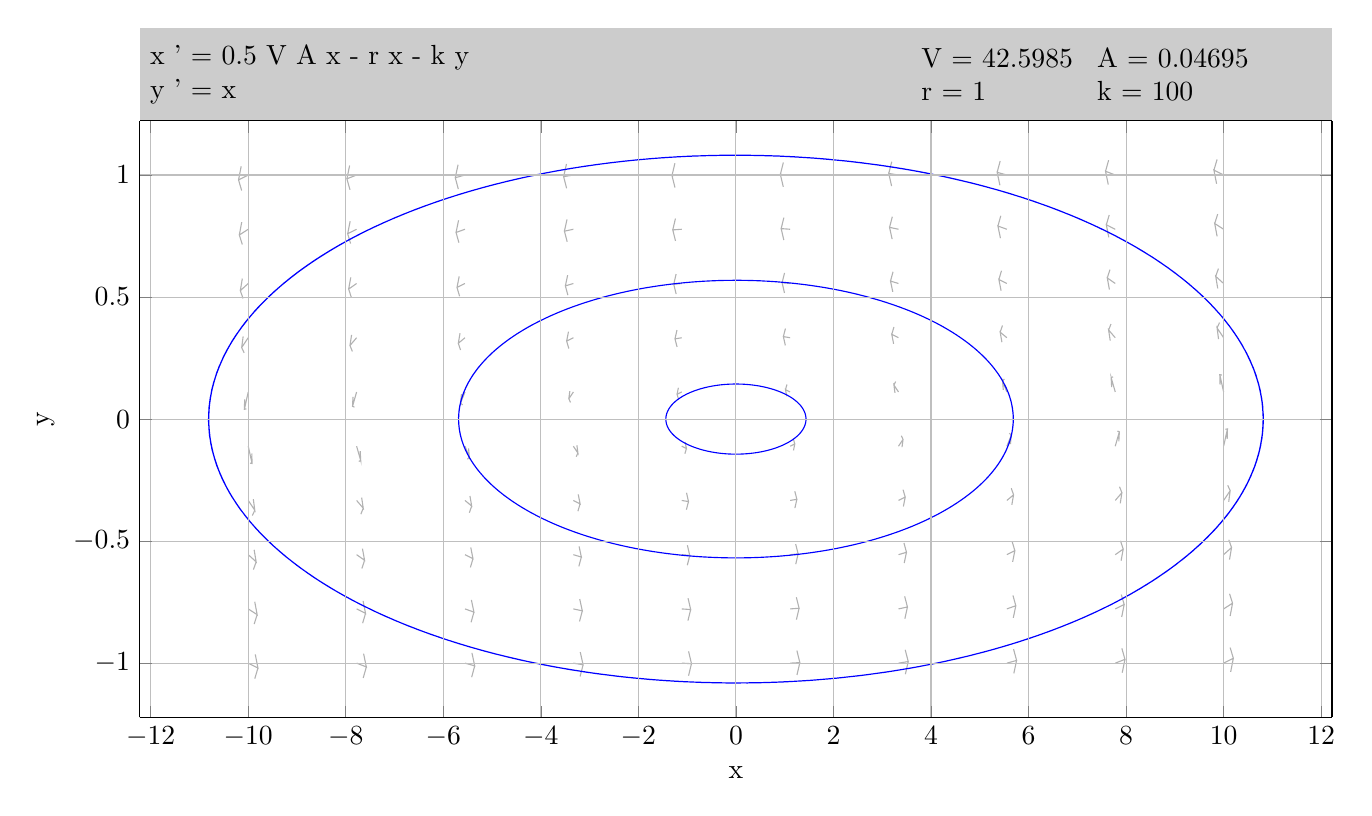
\begin{tikzpicture}

\begin{axis}[%
width=5.960653in,
height=0.465593in,
at={(0.602431in,3.953599in)},
scale only axis,
every outer x axis line/.append style={black},
every x tick label/.append style={font=\color{black}},
xmin=0,
xmax=1,
xtick={-1},
xticklabels={\empty},
every outer y axis line/.append style={black},
every y tick label/.append style={font=\color{black}},
ymin=0,
ymax=1,
ytick={-1},
yticklabels={\empty},
hide axis,
axis background/.style={fill=white!80!black},
axis x line*=bottom,
axis y line*=left
]
\node[right, align=left, inner sep=0mm, text=black]
at (axis cs:0.00806451612903225,0.495614035087719,0) {x ' = 0.5 V A x - r x - k y\\y ' = x};
\node[right, align=left, inner sep=0mm, text=black]
at (axis cs:0.80260034904014,0.5,0) {A = 0.04695\\k = 100};
\node[right, align=left, inner sep=0mm, text=black]
at (axis cs:0.655200698080279,0.5,0) {V = 42.5985\\r = 1};
\node[right, align=left, inner sep=0mm, text=black]
at (axis cs:0.624729493891798,0.5,0) { \\ };
\end{axis}

\begin{axis}[%
width=5.960653in,
height=2.982955in,
at={(0.602431in,0.970644in)},
scale only axis,
unbounded coords=jump,
separate axis lines,
every outer x axis line/.append style={black},
every x tick label/.append style={font=\color{black}},
xmin=-12.2222222222222,
xmax=12.2222222222222,
xlabel={x},
xmajorgrids,
every outer y axis line/.append style={black},
every y tick label/.append style={font=\color{black}},
ymin=-1.22222222222222,
ymax=1.22222222222222,
ylabel={y},
ymajorgrids,
every outer z axis line/.append style={black},
every z tick label/.append style={font=\color{black}},
zmin=-1,
zmax=1,
view={0}{90}
]
\addplot [color=white!70!black,solid,forget plot]
  table[row sep=crcr]{%
-10	-1\\
-9.80099256191613	-1.0199007433855\\
-9.85571960749492	-0.96417866084888\\
-9.80099256191613	-1.0199007433855\\
-9.86566997918767	-1.06368237989081\\
nan	0\\
-10	-0.777777777777778\\
-9.81737728682081	-0.801257840259308\\
-9.86629408515418	-0.748558143220051\\
-9.81737728682081	-0.801257840259308\\
-9.87803411639495	-0.839869499809646\\
nan	0\\
-10	-0.555555555555556\\
-9.83759367618969	-0.584788692723244\\
-9.87900728904086	-0.53541717062036\\
-9.83759367618969	-0.584788692723244\\
-9.89362385762471	-0.616620332525515\\
nan	0\\
-10	-0.333333333333333\\
-9.86547783233039	-0.37368998106148\\
-9.89574532069924	-0.327952444825634\\
-9.86547783233039	-0.37368998106148\\
-9.91592364456331	-0.395213528660438\\
nan	0\\
-10	-0.111111111111111\\
-9.92123448420009	-0.182000061773522\\
-9.92714190127446	-0.14104199762482\\
-9.92123448420009	-0.182000061773522\\
-9.96258637660566	-0.180424755524777\\
nan	0\\
-10	0.111111111111111\\
-10.0787654967689	0.0402221504615824\\
-10.0374136075759	0.0417974644642146\\
-10.0787654967689	0.0402221504615824\\
-10.0728580879006	0.0811802128486674\\
nan	0\\
-10	0.333333333333333\\
-10.1345221610083	0.292976682458109\\
-10.084076349987	0.271453137468603\\
-10.1345221610083	0.292976682458109\\
-10.1042546754246	0.338714217972749\\
nan	0\\
-10	0.555555555555555\\
-10.162406319409	0.526322416943766\\
-10.1063761389334	0.49449077867505\\
-10.162406319409	0.526322416943766\\
-10.1209927082393	0.575693938379555\\
nan	0\\
-10	0.777777777777778\\
-10.1826227097447	0.754297714454812\\
-10.1219658809905	0.715686056015536\\
-10.1826227097447	0.754297714454812\\
-10.133705912652	0.806997410887868\\
nan	0\\
-10	1\\
-10.1990074352088	0.980099256056232\\
-10.1343300186602	0.93631762043717\\
-10.1990074352088	0.980099256056232\\
-10.1442803906321	1.03582133804155\\
nan	0\\
-7.77777777777778	-1\\
-7.57851018865711	-1.01549859000878\\
-7.63441581789111	-0.961032115725981\\
-7.57851018865711	-1.01549859000878\\
-7.6421651128955	-1.06066591028632\\
nan	0\\
-7.77777777777778	-0.777777777777778\\
-7.59476230037469	-0.796079325129178\\
-7.64509155675777	-0.744834991572987\\
-7.59476230037469	-0.796079325129178\\
-7.65424233043347	-0.836342730274529\\
nan	0\\
-7.77777777777778	-0.555555555555556\\
-7.61469466554042	-0.578387190589545\\
-7.65791169045313	-0.530766922020008\\
-7.61469466554042	-0.578387190589545\\
-7.66932750797012	-0.612308478138688\\
nan	0\\
-7.77777777777778	-0.333333333333333\\
-7.64176027858743	-0.365070748237433\\
-7.67463117461851	-0.321545148968617\\
-7.64176027858743	-0.365070748237433\\
-7.69049988207056	-0.389553898563789\\
nan	0\\
-7.77777777777778	-0.111111111111111\\
-7.69373503706152	-0.169941020861541\\
-7.70424038183879	-0.131281362757348\\
-7.69373503706152	-0.169941020861541\\
-7.73365533671401	-0.173302733115476\\
nan	0\\
-7.77777777777778	0.111111111111111\\
-7.86182050467822	0.0522811935298542\\
-7.82190020721277	0.0489194870791218\\
-7.86182050467822	0.0522811935298542\\
-7.8513151660034	0.0909408505293409\\
nan	0\\
-7.77777777777778	0.333333333333333\\
-7.91379527200769	0.301595916439374\\
-7.86505566951522	0.277112767950085\\
-7.91379527200769	0.301595916439374\\
-7.8809243779622	0.345121515065039\\
nan	0\\
-7.77777777777778	0.555555555555555\\
-7.9408608866563	0.532723919633321\\
-7.88622804501219	0.49880263319036\\
-7.9408608866563	0.532723919633321\\
-7.8976438629733	0.580344187629622\\
nan	0\\
-7.77777777777778	0.777777777777778\\
-7.9607932525368	0.759476229912967\\
-7.90131322314289	0.719212825582654\\
-7.9607932525368	0.759476229912967\\
-7.9104639970753	0.810720562962167\\
nan	0\\
-7.77777777777778	1\\
-7.97704536467641	0.984501409651727\\
-7.91339044101975	0.939334090031551\\
-7.97704536467641	0.984501409651727\\
-7.92113973619389	1.03896788348087\\
nan	0\\
-5.55555555555556	-1\\
-5.35609195769038	-1.01108131086169\\
-5.41316070933451	-0.957891018136889\\
-5.35609195769038	-1.01108131086169\\
-5.41870136476536	-1.05762281706947\\
nan	0\\
-5.55555555555556	-0.777777777777778\\
-5.37224327611035	-0.79087151182512\\
-5.42396352643208	-0.741115321749616\\
-5.37224327611035	-0.79087151182512\\
-5.43051039345575	-0.832771461472218\\
nan	0\\
-5.55555555555556	-0.555555555555556\\
-5.39195737332755	-0.57191537343071\\
-5.43694687352717	-0.526107882511163\\
-5.39195737332755	-0.57191537343071\\
-5.44512678246474	-0.607906973625164\\
nan	0\\
-5.55555555555556	-0.333333333333333\\
-5.41837171942604	-0.35619730521182\\
-5.45381087729527	-0.315042154615895\\
-5.41837171942604	-0.35619730521182\\
-5.46524286323452	-0.383634072680653\\
nan	0\\
-5.55555555555556	-0.111111111111111\\
-5.46644572639698	-0.155666020956441\\
-5.48203994768322	-0.120022090713198\\
-5.46644572639698	-0.155666020956441\\
-5.50431740260588	-0.164577005292487\\
nan	0\\
-5.55555555555556	0.111111111111111\\
-5.64466537587741	0.0665561962162243\\
-5.60679370105713	0.0576452156042268\\
-5.64466537587741	0.0665561962162243\\
-5.62907115850458	0.102200125765154\\
nan	0\\
-5.55555555555556	0.333333333333333\\
-5.69273938827092	0.31046936040434\\
-5.64586824522406	0.283032594104196\\
-5.69273938827092	0.31046936040434\\
-5.65730023168856	0.35162451046188\\
nan	0\\
-5.55555555555556	0.555555555555555\\
-5.71915373542002	0.539195737221462\\
-5.66598432687716	0.503204137755573\\
-5.71915373542002	0.539195737221462\\
-5.67416423604421	0.585003227687807\\
nan	0\\
-5.55555555555556	0.777777777777778\\
-5.73886783312698	0.764684043466789\\
-5.68060071627781	0.722784094367228\\
-5.73886783312698	0.764684043466789\\
-5.6871475834333	0.814440233152942\\
nan	0\\
-5.55555555555556	1\\
-5.75501915184121	0.98891868896442\\
-5.69240974519662	0.942377183203679\\
-5.75501915184121	0.98891868896442\\
-5.69795040071441	1.04210898134651\\
nan	0\\
-3.33333333333333	-1\\
-3.13373863368348	-1.00665315660787\\
-3.19195375442647	-0.954758534713045\\
-3.13373863368348	-1.00665315660787\\
-3.1952803327304	-1.05455588453797\\
nan	0\\
-3.33333333333333	-0.777777777777778\\
-3.14982211247942	-0.785642544314177\\
-3.20290928710149	-0.737405309139779\\
-3.14982211247942	-0.785642544314177\\
-3.20684167036969	-0.829160919566735\\
nan	0\\
-3.33333333333333	-0.555555555555556\\
-3.16938813067322	-0.565392267589744\\
-3.2161125134627	-0.521454953314459\\
-3.16938813067322	-0.565392267589744\\
-3.2210308694798	-0.603427554644517\\
nan	0\\
-3.33333333333333	-0.333333333333333\\
-3.19534928245825	-0.347131738127626\\
-3.2332948965222	-0.308496203970567\\
-3.19534928245825	-0.347131738127626\\
-3.24019409891935	-0.37748822940811\\
nan	0\\
-3.33333333333333	-0.111111111111111\\
-3.24006087172952	-0.139092847808418\\
-3.26104717603634	-0.107380211398274\\
-3.24006087172952	-0.139092847808418\\
-3.27503804438499	-0.154016442200179\\
nan	0\\
-3.33333333333333	0.111111111111111\\
-3.42660579031844	0.0831293722317417\\
-3.39162861850307	0.0682057796492746\\
-3.42660579031844	0.0831293722317417\\
-3.40561948794275	0.114842008141831\\
nan	0\\
-3.33333333333333	0.333333333333333\\
-3.47131738221494	0.319534928151957\\
-3.42647256625511	0.289178437485969\\
-3.47131738221494	0.319534928151957\\
-3.4333717688458	0.358170461926771\\
nan	0\\
-3.33333333333333	0.555555555555555\\
-3.49727853458992	0.545718843354742\\
-3.44563579616274	0.50768355670084\\
-3.49727853458992	0.545718843354742\\
-3.45055415226315	0.589656157329132\\
nan	0\\
-3.33333333333333	0.777777777777778\\
-3.51684455306898	0.769913011146053\\
-3.45982499549036	0.726394636201657\\
-3.51684455306898	0.769913011146053\\
-3.46375737880622	0.818150246069483\\
nan	0\\
-3.33333333333333	1\\
-3.53292803203856	0.993346843329366\\
-3.47138633325934	0.945444115654249\\
-3.53292803203856	0.993346843329366\\
-3.47471291159465	1.04524146500686\\
nan	0\\
-1.11111111111111	-1\\
-0.911450731314515	-1.00221844865917\\
-0.970794233088701	-0.951637819112269\\
-0.911450731314515	-1.00221844865917\\
-0.971903457418286	-1.05146800901057\\
nan	0\\
-1.11111111111111	-0.777777777777778\\
-0.927500095235737	-0.78040079228232\\
-0.981927646372213	-0.733711133962114\\
-0.927500095235737	-0.78040079228232\\
-0.983239153624484	-0.825516641899801\\
nan	0\\
-1.11111111111111	-0.555555555555556\\
-0.946991290013525	-0.558837951963557\\
-0.9954066372408	-0.51682327776676\\
-0.946991290013525	-0.558837951963557\\
-0.997047835444801	-0.598883188315553\\
nan	0\\
-1.11111111111111	-0.333333333333333\\
-0.972719875808257	-0.337946374477419\\
-1.01308398611309	-0.30196465330848\\
-0.972719875808257	-0.337946374477419\\
-1.01539050668513	-0.371160270959907\\
nan	0\\
-1.11111111111111	-0.111111111111111\\
-1.0154383137563	-0.120678390643288\\
-1.0417483330797	-0.0938900074449316\\
-1.0154383137563	-0.120678390643288\\
-1.04653197284579	-0.141726406122338\\
nan	0\\
-1.11111111111111	0.111111111111111\\
-1.20678390708372	0.101543831310546\\
-1.1756902483418	0.080495816257563\\
-1.20678390708372	0.101543831310546\\
-1.18047388824208	0.128332214243867\\
nan	0\\
-1.11111111111111	0.333333333333333\\
-1.249502345759	0.328720292145728\\
-1.20683171506773	0.295506395840037\\
-1.249502345759	0.328720292145728\\
-1.20913823566153	0.364702013163982\\
nan	0\\
-1.11111111111111	0.555555555555555\\
-1.27523093174332	0.552273159128961\\
-1.22517438644701	0.512227922898887\\
-1.27523093174332	0.552273159128961\\
-1.2268155846603	0.594287833214991\\
nan	0\\
-1.11111111111111	0.777777777777778\\
-1.29472212661474	0.77515476326262\\
-1.23898306833486	0.73003891374126\\
-1.29472212661474	0.77515476326262\\
-1.24029457559244	0.821844421493075\\
nan	0\\
-1.11111111111111	1\\
-1.31077149059335	0.997781551333848\\
-1.25031876458214	0.948531991063134\\
-1.31077149059335	0.997781551333848\\
-1.25142798891522	1.04836218080425\\
nan	0\\
1.11111111111111	-1\\
1.31077149059335	-0.997781551333848\\
1.25031876458214	-0.948531991063134\\
1.31077149059335	-0.997781551333848\\
1.25142798891522	-1.04836218080425\\
nan	0\\
1.11111111111111	-0.777777777777778\\
1.29472212661474	-0.77515476326262\\
1.23898306833486	-0.73003891374126\\
1.29472212661474	-0.77515476326262\\
1.24029457559244	-0.821844421493075\\
nan	0\\
1.11111111111111	-0.555555555555556\\
1.27523093174332	-0.552273159128961\\
1.22517438644701	-0.512227922898888\\
1.27523093174332	-0.552273159128961\\
1.2268155846603	-0.594287833214991\\
nan	0\\
1.11111111111111	-0.333333333333333\\
1.249502345759	-0.328720292145728\\
1.20683171506773	-0.295506395840037\\
1.249502345759	-0.328720292145728\\
1.20913823566153	-0.364702013163982\\
nan	0\\
1.11111111111111	-0.111111111111111\\
1.20678390708372	-0.101543831310546\\
1.1756902483418	-0.080495816257563\\
1.20678390708372	-0.101543831310546\\
1.18047388824208	-0.128332214243867\\
nan	0\\
1.11111111111111	0.111111111111111\\
1.0154383137563	0.120678390643288\\
1.0417483330797	0.0938900074449316\\
1.0154383137563	0.120678390643288\\
1.04653197284579	0.141726406122338\\
nan	0\\
1.11111111111111	0.333333333333333\\
0.972719875808257	0.337946374477419\\
1.01308398611309	0.30196465330848\\
0.972719875808257	0.337946374477419\\
1.01539050668513	0.371160270959907\\
nan	0\\
1.11111111111111	0.555555555555555\\
0.946991290013525	0.558837951963557\\
0.9954066372408	0.51682327776676\\
0.946991290013525	0.558837951963557\\
0.997047835444801	0.598883188315553\\
nan	0\\
1.11111111111111	0.777777777777778\\
0.927500095235737	0.78040079228232\\
0.981927646372213	0.733711133962114\\
0.927500095235737	0.78040079228232\\
0.983239153624484	0.825516641899801\\
nan	0\\
1.11111111111111	1\\
0.911450731314515	1.00221844865917\\
0.970794233088701	0.951637819112269\\
0.911450731314515	1.00221844865917\\
0.971903457418286	1.05146800901057\\
nan	0\\
3.33333333333333	-1\\
3.53292803203856	-0.993346843329366\\
3.47138633325934	-0.945444115654249\\
3.53292803203856	-0.993346843329366\\
3.47471291159465	-1.04524146500686\\
nan	0\\
3.33333333333333	-0.777777777777778\\
3.51684455306899	-0.769913011146053\\
3.45982499549036	-0.726394636201657\\
3.51684455306899	-0.769913011146053\\
3.46375737880622	-0.818150246069483\\
nan	0\\
3.33333333333333	-0.555555555555556\\
3.49727853458992	-0.545718843354742\\
3.44563579616274	-0.50768355670084\\
3.49727853458992	-0.545718843354742\\
3.45055415226315	-0.589656157329132\\
nan	0\\
3.33333333333333	-0.333333333333333\\
3.47131738221494	-0.319534928151957\\
3.42647256625511	-0.289178437485969\\
3.47131738221494	-0.319534928151957\\
3.4333717688458	-0.358170461926771\\
nan	0\\
3.33333333333333	-0.111111111111111\\
3.42660579031845	-0.0831293722317417\\
3.39162861850307	-0.0682057796492746\\
3.42660579031845	-0.0831293722317417\\
3.40561948794275	-0.114842008141831\\
nan	0\\
3.33333333333333	0.111111111111111\\
3.24006087172952	0.139092847808418\\
3.26104717603634	0.107380211398274\\
3.24006087172952	0.139092847808418\\
3.27503804438499	0.154016442200179\\
nan	0\\
3.33333333333333	0.333333333333333\\
3.19534928245825	0.347131738127626\\
3.2332948965222	0.308496203970567\\
3.19534928245825	0.347131738127626\\
3.24019409891935	0.377488229408109\\
nan	0\\
3.33333333333333	0.555555555555555\\
3.16938813067322	0.565392267589744\\
3.21611251346271	0.521454953314459\\
3.16938813067322	0.565392267589744\\
3.2210308694798	0.603427554644517\\
nan	0\\
3.33333333333333	0.777777777777778\\
3.14982211247942	0.785642544314177\\
3.2029092871015	0.737405309139779\\
3.14982211247942	0.785642544314177\\
3.2068416703697	0.829160919566735\\
nan	0\\
3.33333333333333	1\\
3.13373863368348	1.00665315660787\\
3.19195375442647	0.954758534713045\\
3.13373863368348	1.00665315660787\\
3.1952803327304	1.05455588453797\\
nan	0\\
5.55555555555556	-1\\
5.75501915184122	-0.98891868896442\\
5.69240974519662	-0.942377183203679\\
5.75501915184122	-0.98891868896442\\
5.69795040071441	-1.04210898134651\\
nan	0\\
5.55555555555556	-0.777777777777778\\
5.73886783312699	-0.764684043466789\\
5.68060071627781	-0.722784094367228\\
5.73886783312699	-0.764684043466789\\
5.6871475834333	-0.814440233152942\\
nan	0\\
5.55555555555556	-0.555555555555556\\
5.71915373542003	-0.539195737221463\\
5.66598432687716	-0.503204137755573\\
5.71915373542003	-0.539195737221463\\
5.67416423604421	-0.585003227687808\\
nan	0\\
5.55555555555556	-0.333333333333333\\
5.69273938827093	-0.31046936040434\\
5.64586824522407	-0.283032594104196\\
5.69273938827093	-0.31046936040434\\
5.65730023168856	-0.35162451046188\\
nan	0\\
5.55555555555556	-0.111111111111111\\
5.64466537587741	-0.0665561962162243\\
5.60679370105713	-0.0576452156042268\\
5.64466537587741	-0.0665561962162243\\
5.62907115850458	-0.102200125765154\\
nan	0\\
5.55555555555556	0.111111111111111\\
5.46644572639698	0.155666020956441\\
5.48203994768322	0.120022090713198\\
5.46644572639698	0.155666020956441\\
5.50431740260589	0.164577005292487\\
nan	0\\
5.55555555555556	0.333333333333333\\
5.41837171942604	0.35619730521182\\
5.45381087729527	0.315042154615895\\
5.41837171942604	0.35619730521182\\
5.46524286323452	0.383634072680653\\
nan	0\\
5.55555555555556	0.555555555555555\\
5.39195737332755	0.57191537343071\\
5.43694687352717	0.526107882511162\\
5.39195737332755	0.57191537343071\\
5.44512678246474	0.607906973625164\\
nan	0\\
5.55555555555556	0.777777777777778\\
5.37224327611035	0.79087151182512\\
5.42396352643208	0.741115321749616\\
5.37224327611035	0.79087151182512\\
5.43051039345575	0.832771461472218\\
nan	0\\
5.55555555555556	1\\
5.35609195769039	1.01108131086169\\
5.41316070933452	0.957891018136889\\
5.35609195769039	1.01108131086169\\
5.41870136476536	1.05762281706947\\
nan	0\\
7.77777777777778	-1\\
7.97704536467641	-0.984501409651727\\
7.91339044101975	-0.939334090031551\\
7.97704536467641	-0.984501409651727\\
7.92113973619389	-1.03896788348087\\
nan	0\\
7.77777777777778	-0.777777777777778\\
7.9607932525368	-0.759476229912967\\
7.90131322314289	-0.719212825582655\\
7.9607932525368	-0.759476229912967\\
7.9104639970753	-0.810720562962167\\
nan	0\\
7.77777777777778	-0.555555555555556\\
7.9408608866563	-0.532723919633321\\
7.88622804501219	-0.49880263319036\\
7.9408608866563	-0.532723919633321\\
7.8976438629733	-0.580344187629622\\
nan	0\\
7.77777777777778	-0.333333333333333\\
7.91379527200769	-0.301595916439374\\
7.86505566951523	-0.277112767950085\\
7.91379527200769	-0.301595916439374\\
7.8809243779622	-0.345121515065039\\
nan	0\\
7.77777777777778	-0.111111111111111\\
7.86182050467822	-0.0522811935298542\\
7.82190020721277	-0.0489194870791218\\
7.86182050467822	-0.0522811935298542\\
7.8513151660034	-0.0909408505293408\\
nan	0\\
7.77777777777778	0.111111111111111\\
7.69373503706152	0.169941020861541\\
7.70424038183879	0.131281362757348\\
7.69373503706152	0.169941020861541\\
7.73365533671401	0.173302733115476\\
nan	0\\
7.77777777777778	0.333333333333333\\
7.64176027858744	0.365070748237433\\
7.67463117461851	0.321545148968617\\
7.64176027858744	0.365070748237433\\
7.69049988207056	0.389553898563789\\
nan	0\\
7.77777777777778	0.555555555555555\\
7.61469466554042	0.578387190589545\\
7.65791169045313	0.530766922020008\\
7.61469466554042	0.578387190589545\\
7.66932750797012	0.612308478138688\\
nan	0\\
7.77777777777778	0.777777777777778\\
7.59476230037469	0.796079325129178\\
7.64509155675777	0.744834991572987\\
7.59476230037469	0.796079325129178\\
7.65424233043347	0.836342730274529\\
nan	0\\
7.77777777777778	1\\
7.57851018865711	1.01549859000878\\
7.63441581789111	0.961032115725981\\
7.57851018865711	1.01549859000878\\
7.64216511289551	1.06066591028632\\
nan	0\\
10	-1\\
10.1990074352088	-0.980099256056232\\
10.1343300186602	-0.93631762043717\\
10.1990074352088	-0.980099256056232\\
10.1442803906321	-1.03582133804155\\
nan	0\\
10	-0.777777777777778\\
10.1826227097447	-0.754297714454812\\
10.1219658809905	-0.715686056015536\\
10.1826227097447	-0.754297714454812\\
10.133705912652	-0.806997410887868\\
nan	0\\
10	-0.555555555555556\\
10.162406319409	-0.526322416943766\\
10.1063761389334	-0.494490778675051\\
10.162406319409	-0.526322416943766\\
10.1209927082393	-0.575693938379556\\
nan	0\\
10	-0.333333333333333\\
10.1345221610083	-0.292976682458109\\
10.084076349987	-0.271453137468603\\
10.1345221610083	-0.292976682458109\\
10.1042546754246	-0.33871421797275\\
nan	0\\
10	-0.111111111111111\\
10.0787654967689	-0.0402221504615824\\
10.0374136075759	-0.0417974644642146\\
10.0787654967689	-0.0402221504615824\\
10.0728580879006	-0.0811802128486674\\
nan	0\\
10	0.111111111111111\\
9.92123448420009	0.182000061773522\\
9.92714190127446	0.14104199762482\\
9.92123448420009	0.182000061773522\\
9.96258637660566	0.180424755524777\\
nan	0\\
10	0.333333333333333\\
9.86547783233039	0.37368998106148\\
9.89574532069924	0.327952444825633\\
9.86547783233039	0.37368998106148\\
9.91592364456331	0.395213528660438\\
nan	0\\
10	0.555555555555555\\
9.83759367618969	0.584788692723244\\
9.87900728904086	0.53541717062036\\
9.83759367618969	0.584788692723244\\
9.89362385762471	0.616620332525514\\
nan	0\\
10	0.777777777777778\\
9.81737728682081	0.801257840259308\\
9.86629408515418	0.748558143220051\\
9.81737728682081	0.801257840259308\\
9.87803411639495	0.839869499809646\\
nan	0\\
10	1\\
9.80099256191613	1.0199007433855\\
9.85571960749492	0.96417866084888\\
9.80099256191613	1.0199007433855\\
9.86566997918767	1.06368237989081\\
nan	0\\
};
\addplot3 [color=blue,solid]
 table[row sep=crcr] {%
-1.08974358974359	0.0936895083236551	0\\
-1.11094845764074	0.0911650716500949	0.00229411764705883\\
-1.1315686834306	0.0885926553780006	0.00458823529411766\\
-1.151593377016	0.0859736167646501	0.00688235294117648\\
-1.17101198434257	0.0833093352465183	0.00917647058823531\\
-1.18981428739878	0.0806012124392779	0.0114705882352941\\
-1.20799040421588	0.0778506721377989	0.013764705882353\\
-1.22553078886793	0.0750591603161489	0.0160588235294118\\
-1.24242623147182	0.0722281451275926	0.0183529411764706\\
-1.28565917727259	0.0642184926821751	0.0246870334370418\\
-1.32373979303399	0.0559510217925656	0.0310211256976129\\
-1.35650902570524	0.0474594168439177	0.0373552179581841\\
-1.38383230745284	0.0387778713500216	0.0436893102187552\\
-1.40559955566063	0.0299410879533043	0.0500234024793264\\
-1.42172517292975	0.0209842784248295	0.0563574947398975\\
-1.43214804707867	0.0119431636642975	0.0626915870004687\\
-1.43683155114318	0.00285397370004542	0.0690256792610398\\
-1.43629846781184	-0.0048465587739312	0.074384586545643\\
-1.43164249215365	-0.0125333615410393	0.0797434938302461\\
-1.42287588717471	-0.0201840255456471	0.0851024011148492\\
-1.41002305224865	-0.0277764640362485	0.0904613083994524\\
-1.39312052311661	-0.0352889125654636	0.0958202156840555\\
-1.37221697188727	-0.0426999289900381	0.101179122968659\\
-1.34737320703685	-0.0499883934708437	0.106538030253262\\
-1.31866217340906	-0.0571335084728779	0.111896937537865\\
-1.28936693125971	-0.0634687454496803	0.116754105230072\\
-1.25703036769481	-0.0696543995675498	0.12161127292228\\
-1.22172906651389	-0.0756756641203108	0.126468440614487\\
-1.18354621552589	-0.081518250529489	0.131325608306695\\
-1.14257160654911	-0.0871683883443108	0.136182775998902\\
-1.09890163541126	-0.0926128252417039	0.141039943691109\\
-1.05263930194942	-0.0978388270262966	0.145897111383317\\
-1.00389421001005	-0.102834177630419	0.150754279075524\\
-0.94147449381256	-0.108578134752906	0.156657395237315\\
-0.875773872526712	-0.113944158661805	0.162560511399106\\
-0.807023853839124	-0.118913040603698	0.168463627560898\\
-0.735464411157682	-0.123467238527721	0.174366743722689\\
-0.661343983611549	-0.127590877085559	0.18026985988448\\
-0.584919476051158	-0.13126974763145	0.186172976046271\\
-0.506456259048213	-0.134491308222181	0.192076092208062\\
-0.426228168895693	-0.137244683617092	0.197979208369853\\
-0.337369120513804	-0.139695061085249	0.204393822948018\\
-0.247118750915005	-0.141571196495501	0.210808437526182\\
-0.155855227241736	-0.142864838401654	0.217223052104347\\
-0.0639560900455617	-0.143570369714398	0.223637666682511\\
0.0282017467128193	-0.143684807701311	0.230052281260676\\
0.120241995663581	-0.143207803986853	0.23646689583884\\
0.211788996027767	-0.142141644552375	0.242881510417005\\
0.302467713617294	-0.140491249736109	0.249296124995169\\
0.374530326706228	-0.13874419256146	0.25445623346762\\
0.445597564294319	-0.136627819072488	0.25961634194007\\
0.515477291178501	-0.134147742116582	0.26477645041252\\
0.583982361341667	-0.131310527114421	0.26993655888497\\
0.650930617952667	-0.128123692059972	0.27509666735742\\
0.716144893366311	-0.124595707520488	0.28025677582987\\
0.779453009123367	-0.120735996636512	0.28541688430232\\
0.840687775950561	-0.116554935121875	0.290576992774771\\
0.903379555984071	-0.111766265895621	0.296066885022694\\
0.963351601175839	-0.106640784375539	0.301556777270618\\
1.02041938835481	-0.101194062027148	0.307046669518541\\
1.07440934328257	-0.0954425211690875	0.312536561766465\\
1.12515884065335	-0.0894034349731199	0.318026454014388\\
1.17251620409404	-0.0830949274641299	0.323516346262312\\
1.21634070616417	-0.076535973520124	0.329006238510235\\
1.2565025683559	-0.0697463988722309	0.334496130758159\\
1.29802789404237	-0.0616754202262133	0.340812656561782\\
1.33437999599824	-0.0533581875589693	0.347129182365405\\
1.36540775771117	-0.0448284057808007	0.353445708169028\\
1.39098435966454	-0.0361202367221496	0.359762233972652\\
1.41100727933743	-0.0272682991335985	0.366078759776275\\
1.42539829120465	-0.01830766868587	0.372395285579898\\
1.4341034667367	-0.00927387796982706	0.378711811383521\\
1.43709317439981	-0.00020291649647268	0.385028337187144\\
1.43520807027592	0.00736288577610399	0.39029505708023\\
1.42934360734208	0.0149084407893252	0.395561776973316\\
1.41951510973289	0.02241250965937	0.400828496866402\\
1.40574915958086	0.0298541697603562	0.406095216759488\\
1.38808359701638	0.0372128147243405	0.411361936652573\\
1.3665675201677	0.0444681544413185	0.416628656545659\\
1.34126128516099	0.0516002150592245	0.421895376438745\\
1.31223650612028	0.0585893389839319	0.427162096331831\\
1.28238785646704	0.0648628242680889	0.431996779578547\\
1.24954226701308	0.0709848483804904	0.436831462825262\\
1.21377682569007	0.0769408934046716	0.441666146071978\\
1.17517504896837	0.0827169562748799	0.446500829318694\\
1.13382688185704	0.0882995487760752	0.451335512565409\\
1.08982869790384	0.0936756975439296	0.456170195812125\\
1.04328329919522	0.0988329440648275	0.461004879058841\\
0.994299916356322	0.103759344675866	0.465839562305556\\
0.931120998696761	0.109464662799147	0.471763693677255\\
0.864674068620264	0.1147862451048	0.477687825048954\\
0.795194973550117	0.119704898431482	0.483611956420652\\
0.722927978903567	0.124203129554983	0.489536087792351\\
0.64812576809182	0.128265145188226	0.49546021916405\\
0.571049442520045	0.131876851981267	0.501384350535749\\
0.491968521587372	0.135025856521297	0.507308481907447\\
0.41116094268689	0.137701465332639	0.513232613279146\\
0.322567563129985	0.140042162345764	0.519609570909251\\
0.232659333233192	0.141813914837976	0.525986528539356\\
0.141808551494208	0.143009010373195	0.532363486169462\\
0.0503866631003236	0.143622306718884	0.538740443799567\\
-0.0412357400715705	0.143651231846051	0.545117401429672\\
-0.132688919454988	0.143095783929243	0.551494359059777\\
-0.223603989793844	0.141958531346555	0.557871316689882\\
-0.313612919142459	0.140244612679621	0.564248274319987\\
-0.385364891133967	0.138445089858782	0.569396206724845\\
-0.456097462593577	0.136278782003085	0.574544139129703\\
-0.525620309522583	0.133751410474954	0.57969207153456\\
-0.593748118504736	0.130869636342539	0.584840003939418\\
-0.660300586706244	0.127641060379717	0.589987936344275\\
-0.725102421875775	0.124074223066093	0.595135868749133\\
-0.787983342344451	0.120178604587001	0.600283801153991\\
-0.848778077025857	0.115964624833499	0.605431733558848\\
-0.911339855068811	0.111115552194872	0.610940168310828\\
-0.97113937356	0.105929360950634	0.616448603062807\\
-1.02799135324381	0.100421915666135	0.621957037814786\\
-1.08172168333337	0.0946099349420716	0.627465472566766\\
-1.13216742151055	0.0885109914144883	0.632973907318745\\
-1.17917679392597	0.0821435117547767	0.638482342070725\\
-1.22260919519898	0.0755267766696751	0.643990776822704\\
-1.26233518841769	0.0686809209012689	0.649499211574683\\
-1.3032500180052	0.0605593868731712	0.655827903345154\\
-1.33895077902356	0.0521951134677012	0.662156595115625\\
-1.36928838676096	0.0436221317072693	0.668485286886096\\
-1.39413828761038	0.0348749112272457	0.674813978656566\\
-1.41340045906957	0.0259883602759602	0.681142670427037\\
-1.42699940974102	0.0169978257147023	0.687471362197508\\
-1.43488417933201	0.00793909301772117	0.693800053967979\\
-1.43702833865459	-0.00115161372777448	0.700128745738449\\
-1.43443802911668	-0.00870234848217766	0.705386509767322\\
-1.42788398673295	-0.016229202626841	0.710644273796195\\
-1.4173834251142	-0.0237110617989856	0.715902037825068\\
-1.40296470860763	-0.0311271357594244	0.72115980185394\\
-1.38466735229688	-0.0384569583925616	0.726417565882813\\
-1.36254202200201	-0.0456803877063936	0.731675329911686\\
-1.3366505342795	-0.0527776058325078	0.736933093940559\\
-1.30706585642227	-0.0597291190260841	0.742190857969431\\
-1.27646636037893	-0.0660161425862018	0.747056760397047\\
-1.24284511131204	-0.0721470152311426	0.751922662824663\\
-1.20628205352591	-0.0781070061233329	0.756788565252279\\
-1.16686367711774	-0.0838819196839832	0.761654467679895\\
-1.12468301797762	-0.0894580955930878	0.766520370107511\\
-1.07983965778855	-0.0948224087894251	0.771386272535127\\
-1.03243972402641	-0.0999622694705572	0.776252174962743\\
-0.982595889959974	-0.10486562309283	0.781118077390359\\
-0.918577208272306	-0.110516770303078	0.787060780029799\\
-0.851314241027918	-0.11577806023865	0.793003482669239\\
-0.781047276639191	-0.120630390005449	0.798946185308679\\
-0.708024923450605	-0.125056388819186	0.804888887948119\\
-0.632504109738742	-0.129040418005384	0.810831590587559\\
-0.554750083712288	-0.132568570999371	0.816774293226999\\
-0.475036413512028	-0.135628673346288	0.822716995866439\\
-0.393644987210847	-0.138210282701081	0.828659698505879\\
-0.305397606660973	-0.140424515450453	0.83499147290556\\
-0.215922774355375	-0.142076289205264	0.84132324730524\\
-0.125585729756837	-0.143158501934426	0.84765502170492\\
-0.0347506136207802	-0.143666546208342	0.8539867961046\\
0.0562195320047367	-0.143598309198906	0.86031857050428\\
0.146962763779018	-0.142954172679502	0.866650344903961\\
0.237118237068731	-0.141737013025003	0.872982119303641\\
0.326326205947906	-0.139952201211775	0.879313893703321\\
0.397714116954802	-0.138093312237628	0.884447580175744\\
0.468055710379168	-0.135870589994097	0.889581266648166\\
0.537162766425856	-0.13328987586796	0.894714953120589\\
0.6048520973308	-0.130357936120167	0.899848639593012\\
0.670945547361018	-0.127082461885839	0.904982326065435\\
0.73526999281461	-0.123472069174266	0.910116012537857\\
0.797657342020756	-0.11953629886891	0.91524969901028\\
0.857944535339721	-0.115285616727403	0.920383385482703\\
0.920349407317701	-0.11036786179846	0.925912728751504\\
0.979943501806053	-0.105112708138858	0.931442072020304\\
1.03654072331413	-0.0995363559159953	0.936971415289105\\
1.08996639641742	-0.0936558626319588	0.942500758557906\\
1.14005726575752	-0.0874891431235225	0.948030101826707\\
1.18666149604217	-0.0810549695621478	0.953559445095507\\
1.22963867204523	-0.0743729714539833	0.959088788364308\\
1.26885979860669	-0.067463635639865	0.964618131633109\\
1.30907354592403	-0.0592851986169733	0.970960624506594\\
1.34402705253966	-0.0508680813735757	0.97730311738008\\
1.37357359626878	-0.0422466849720895	0.983645610253566\\
1.39759125155419	-0.0334558278280605	0.989988103127051\\
1.41598288946628	-0.024530745710163	0.996330596000537\\
1.42867617770299	-0.0155070917401999	1.00267308887402\\
1.43562358058985	-0.00642093639310301	1.00901558174751\\
1.43680235907997	0.00269123250306778	1.01535807462099\\
1.43340667354476	0.0102338016842819	1.02061245485596\\
1.4260551809151	0.0177482942739739	1.02586683509092\\
1.41476730948986	0.0252136568360379	1.03112121532589\\
1.39957357398021	0.0326091709257238	1.03637559556085\\
1.38051557550961	0.0399144530896379	1.04162997579582\\
1.35764600161383	0.0471094548657424	1.04688435603078\\
1.33102862624092	0.0541744627833557	1.05213873626575\\
1.30073830975128	0.0610900983631523	1.05739311650071\\
1.26919838355199	0.0673986103091079	1.06230145733183\\
1.23460127133002	0.0735449097144884	1.06720979816295\\
1.19703069603582	0.079513965040977	1.07211813899406\\
1.15657709356454	0.0852913077387415	1.07702647982518\\
1.11333761275604	0.0908630322464345	1.0819348206563\\
1.0674161153949	0.0962157959911931	1.08684316148741\\
1.01892317621039	0.101336819388639	1.09175150231853\\
0.967976082876528	0.106213885842879	1.09665984314964\\
0.90293414753719	0.111795879131656	1.10262474931555\\
0.834679232109693	0.116980549938762	1.10858965548145\\
0.763457050821037	0.121748922619779	1.11455456164735\\
0.689521505621789	0.126083792768729	1.12051946781325\\
0.613134686186076	0.129969727218072	1.12648437397916\\
0.534566869911592	0.133393064038708	1.13244928014506\\
0.454096521919594	0.136341912539976	1.13841418631096\\
0.3720102950549	0.138806153269654	1.14437909247686\\
0.2842147741488	0.140866447489543	1.15065511635394\\
0.195296755640558	0.142372384886981	1.15693114023101\\
0.10561280040547	0.143317586555508	1.16320716410808\\
0.0155180902656005	0.143698076927377	1.16948318798515\\
-0.074633572010212	0.14351228377356	1.17575921186223\\
-0.164489762706356	0.142761038203745	1.1820352357393\\
-0.253699437160447	0.141447574666333	1.18831125961637\\
-0.34191292976333	0.139577530948445	1.19458728349344\\
-0.412848843698202	0.137646326040253	1.19970359417766\\
-0.4827058868163	0.135354913595005	1.20481990486187\\
-0.551298406393802	0.132709278888484	1.20993621554608\\
-0.618445806454726	0.129716314108008	1.2150525262303\\
-0.683972547770927	0.126383818352423	1.22016883691451\\
-0.747708147862096	0.122720497632109	1.22528514759872\\
-0.809487180995759	0.118735964868977	1.23040145828294\\
-0.869149278187285	0.114440739896469	1.23551776896715\\
-0.931347620488591	0.109438741797198	1.24107246193665\\
-0.990675464605378	0.104099108407628	1.24662715490614\\
-1.04694578362812	0.0984384545907662	1.25218184787564\\
-1.0999832817817	0.0924742560837746	1.25773654084514\\
-1.14962439442543	0.086224849497967	1.26329123381464\\
-1.19571728805306	0.0797094323188109	1.26884592678414\\
-1.23812186029274	0.0729480629059273	1.27440061975363\\
-1.27670973990704	0.06596166049309	1.27995531272313\\
-1.31605328725445	0.0577142371446977	1.28631470534074\\
-1.35008032079184	0.0492332048601571	1.29267409795834\\
-1.3786470928006	0.0405534177606518	1.29903349057595\\
-1.4016349771343	0.0317101205868326	1.30539288319355\\
-1.41895046921866	0.0227389486988172	1.31175227581116\\
-1.43052518605161	0.0136759280761904	1.31811166842877\\
-1.43631586620323	0.00455747531800394	1.32447106104637\\
-1.43630436981578	-0.00457960235722348	1.33083045366398\\
-1.43192255071888	-0.0121110630433026	1.33608072275805\\
-1.42359517631691	-0.019609318012753	1.34133099185212\\
-1.41134437761197	-0.0270533911134813	1.34658126094619\\
-1.39520329212904	-0.0344226543980808	1.35183153004026\\
-1.37521606391595	-0.0416968281238309	1.35708179913434\\
-1.35143784354343	-0.048855980752698	1.36233206822841\\
-1.32393478810506	-0.0558805289513347	1.36758233732248\\
-1.2927840612173	-0.0627512375910801	1.37283260641655\\
-1.26009354636234	-0.0690817204366282	1.37779092782749\\
-1.22430564475509	-0.0752425381573852	1.38274924923843\\
-1.18550875576729	-0.0812183092026787	1.38770757064938\\
-1.14379818609725	-0.0869942493575483	1.39266589206032\\
-1.09927614976993	-0.0925561717427457	1.39762421347126\\
-1.05205176813688	-0.0978904868147344	1.4025825348822\\
-1.00224106987626	-0.10298420236569	1.40754085629314\\
-0.94996699099285	-0.1078249235235	1.41249917770409\\
-0.883693485655228	-0.11332034001994	1.41849083205136\\
-0.814247113136128	-0.118409395289414	1.42448248639862\\
-0.741880194631829	-0.123073283729121	1.43047414074589\\
-0.666853066160304	-0.127295018633495	1.43646579509316\\
-0.58943407856122	-0.131059432194207	1.44245744944043\\
-0.509899597495934	-0.134353175500165	1.4484491037877\\
-0.428534003447498	-0.137164718537513	1.45444075813497\\
-0.345629691720655	-0.139484350189633	1.46043241248224\\
-0.258419442866626	-0.141360333260458	1.46664063550684\\
-0.170210241865776	-0.142691947645894	1.47284885853143\\
-0.0813481527446412	-0.143473651243035	1.47905708155603\\
0.00782244929957621	-0.14370219729201	1.48526530458062\\
0.0969588778990065	-0.143376634375979	1.49147352760522\\
0.185720135515114	-0.142498306421139	1.49768175062981\\
0.273766913438697	-0.141070852696722	1.50388997365441\\
0.360761591789887	-0.139100207814991	1.510098196679\\
0.431142724611694	-0.137082227745252	1.51519364585571\\
0.500406261248863	-0.134708432583606	1.52028909503242\\
0.568369632952556	-0.131984976974723	1.52538454420913\\
0.634855355438203	-0.128918901084517	1.53047999338583\\
0.699691028885505	-0.125518130600142	1.53557544256254\\
0.76270933793843	-0.121791476729996	1.54067089173925\\
0.823748051705218	-0.117748636203718	1.54576634091596\\
0.882650023758377	-0.113400191272191	1.55086179009266\\
0.944577757915556	-0.10829625219106	1.55644675094418\\
1.00356241354773	-0.102854548559415	1.5620317117957\\
1.05941593932094	-0.0970922016129841	1.56761667264722\\
1.11196239513418	-0.0910271969914383	1.57320163349874\\
1.16103795211938	-0.0846783847383916	1.57878659435026\\
1.2064908926414	-0.0780654793014008	1.58437155520178\\
1.24818161029807	-0.0712090595319657	1.5899565160533\\
1.28598260992011	-0.0641305686855286	1.59554147690482\\
1.32425773040761	-0.0558008616906357	1.60192129014242\\
1.35714877246703	-0.0472438206080031	1.60830110338002\\
1.38451570235251	-0.0384948466195547	1.61468091661762\\
1.40624400002294	-0.0295896981913909	1.62106072985522\\
1.422244659142	-0.0205644910737884	1.62744054309282\\
1.43245418707813	-0.011455698301201	1.63382035633042\\
1.43683460490452	-0.00230015019225881	1.64020016956802\\
1.43537344739917	0.00686496565023159	1.64657998280562\\
1.42980062089623	0.0143813549488566	1.65182533039143\\
1.42029543797715	0.0218583563420295	1.65707067797724\\
1.4068832806742	0.0292750910362237	1.66231602556305\\
1.38960043934961	0.0366110442637491	1.66756137314886\\
1.36849411269555	0.0438460652827515	1.67280672073467\\
1.34362240773418	0.0509603673772134	1.67805206832048\\
1.3150543398176	0.0579345278569529	1.68329741590629\\
1.28286983262785	0.0647494880576249	1.6885427634921\\
};
 \addplot3 [color=blue,solid]
 table[row sep=crcr] {%
-4.12393162393162	0.391792489353465	0\\
-4.14760685201134	0.389285305490401	0.000606217616580311\\
-4.17112965618823	0.386763815434625	0.00121243523316062\\
-4.19449917181499	0.384228111869034	0.00181865284974093\\
-4.21771453999482	0.381678287986887	0.00242487046632124\\
-4.24077490758141	0.379114437491805	0.00303108808290156\\
-4.263679427179	0.376536654597774	0.00363730569948187\\
-4.28642725714228	0.373945034029139	0.00424352331606218\\
-4.30901756157648	0.37133967102061	0.00484974093264249\\
-4.4839763779758	0.350013246366952	0.00969948186528498\\
-4.64839526558659	0.327863528241062	0.0145492227979275\\
-4.8018804705711	0.304943082609273	0.01939896373057\\
-4.94406789392686	0.281305927114267	0.0242487046632124\\
-5.07462309148671	0.257007531075073	0.0290984455958549\\
-5.19324127391879	0.232104815487075	0.0339481865284974\\
-5.29964730672651	0.206656153022002	0.0387979274611399\\
-5.39359571024861	0.180721368027933	0.0436476683937824\\
-5.49544142558261	0.146871552007563	0.0498625578677034\\
-5.57608038183022	0.11245342423787	0.0560774473416243\\
-5.63518290172286	0.0776022074394753	0.0622923368155453\\
-5.67251081515407	0.0424531855358263	0.0685072262894662\\
-5.6879174591795	0.00714170365319811	0.0747221157633872\\
-5.68134767801691	-0.0281968318793068	0.0809370052373081\\
-5.65283782304618	-0.0634269535297585	0.0871518947112291\\
-5.6025157528093	-0.0984131325634007	0.09336678418515\\
-5.54486488688091	-0.126933193710453	0.0984824162053475\\
-5.47270787437356	-0.155121769006015	0.103598048225545\\
-5.38623230854108	-0.182903991781043	0.108713680245742\\
-5.28566290964119	-0.210206753517353	0.11382931226594\\
-5.1712615249355	-0.236958703847625	0.118944944286137\\
-5.04332712868948	-0.263090250555403	0.124060576306335\\
-4.9021958221725	-0.288533559575092	0.129176208326532\\
-4.7482408336578	-0.313222554991965	0.13429184034673\\
-4.57318725984229	-0.338269573344897	0.139664382554174\\
-4.38493537384147	-0.362341247164947	0.145036924761619\\
-4.1840324781992	-0.385366739905088	0.150409466969063\\
-3.9710585217838	-0.407279031606665	0.155782009176508\\
-3.74662609978804	-0.428014918899393	0.161154551383953\\
-3.51138045372921	-0.447515015001359	0.166527093591397\\
-3.26599947144904	-0.465723749719018	0.171899635798842\\
-3.01119368711372	-0.482589369447198	0.177272178006286\\
-2.70471257549889	-0.500411580303659	0.183505484986426\\
-2.38771700524895	-0.516291632764548	0.189738791966565\\
-2.06145685175693	-0.530165488270088	0.195972098946705\\
-1.72720405175161	-0.541978105217375	0.202205405926844\\
-1.38625260329749	-0.551683438960373	0.208438712906984\\
-1.03991856579482	-0.559244441809921	0.214672019887123\\
-0.68954005997956	-0.564633063033727	0.220905326867263\\
-0.336477267923401	-0.567830248856369	0.227138633847402\\
-0.0241283246757024	-0.568821629021962	0.232632988550483\\
0.288301570527475	-0.568096716419708	0.238127343253565\\
0.599854524071113	-0.565657132595176	0.243621697956646\\
0.909584999019631	-0.561509865514773	0.249116052659727\\
1.21655981511688	-0.555667269565747	0.254610407362808\\
1.51985814878616	-0.548147065556185	0.260104762065889\\
1.81857153313019	-0.538972340715011	0.26559911676897\\
2.11180385793114	-0.528171548691993	0.271093471472052\\
2.36652657963847	-0.517260191875492	0.275965436048032\\
2.6156381889965	-0.50512130778331	0.280837400624013\\
2.85853878420244	-0.491783802705582	0.285709365199994\\
3.09464848454916	-0.477279286287024	0.290581329775974\\
3.32340743042513	-0.461642071526931	0.295453294351955\\
3.54427578331448	-0.444909174779177	0.300325258927936\\
3.75673372579693	-0.427120315752213	0.305197223503916\\
3.96028146154785	-0.408317917509072	0.310069188079897\\
4.19167400658945	-0.384527281039016	0.315904148794706\\
4.40881120732118	-0.359427433092027	0.321739109509515\\
4.61093451853802	-0.333104742820725	0.327574070224324\\
4.797347286729	-0.3056489623124	0.333409030939133\\
4.96741475007718	-0.277153226589014	0.339243991653942\\
5.1205640384597	-0.2477140536072	0.345078952368751\\
5.25628417344774	-0.217431344258262	0.35091391308356\\
5.37412606830651	-0.186408382368176	0.356748873798369\\
5.46334560147278	-0.15836444103369	0.36192294418943\\
5.53794702248696	-0.129896136363105	0.367097014580491\\
5.59772378725259	-0.101080630291524	0.372271084971552\\
5.64251230340643	-0.0719953549398522	0.377445155362612\\
5.67219193031841	-0.0427180126147977	0.382619225753673\\
5.68668497909165	-0.0133265758088727	0.387793296144734\\
5.68595671256243	0.0161007127996075	0.392967366535795\\
5.67001534530024	0.0454853403465254	0.398141436926856\\
5.64078285809793	0.0733185156134468	0.40306183865363\\
5.59789816368588	0.100974718880506	0.407982240380404\\
5.54146332408324	0.128386100896195	0.412902642107177\\
5.47161343219913	0.15548597862435	0.417823043833951\\
5.38851661183268	0.182208835244146	0.422743445560725\\
5.292374017673	0.208490320150103	0.427663847287498\\
5.18341983529918	0.23426724895208	0.432584249014272\\
5.0619212811803	0.259477603475279	0.437504650741046\\
4.92406251233087	0.284772701551832	0.44256951920658\\
4.77357432840155	0.309338036039669	0.447634387672115\\
4.61084476383835	0.333109557415416	0.45269925613765\\
4.43629098144472	0.356025874386576	0.457764124603185\\
4.25035927238155	0.378028253891523	0.46282899306872\\
4.05352505616721	0.399060621099506	0.467893861534255\\
3.84629288067752	0.419069559410648	0.47295872999979\\
3.62919642214573	0.438004310455945	0.478023598465324\\
3.35878260667914	0.459069838953887	0.484050341366114\\
3.07616689651793	0.478469811095947	0.490077084266904\\
2.78238867436753	0.496131614402168	0.496103827167694\\
2.47851746007726	0.511990111365226	0.502130570068484\\
2.16565291064033	0.525987639450428	0.508157312969274\\
1.84492482019383	0.538074011095716	0.514184055870064\\
1.51749312001873	0.548206513711663	0.520210798770854\\
1.18454787853987	0.556349909681473	0.526237541671644\\
0.844768217772451	0.562513418333195	0.53230901405864\\
0.501863496617625	0.566604948490485	0.538380486445636\\
0.157119896572411	0.568608056089397	0.544451958832632\\
-0.188184762729575	0.568514564300615	0.550523431219629\\
-0.532781023518129	0.566324563529453	0.556594903606625\\
-0.875407789886455	0.562046411415861	0.562666375993621\\
-1.21481232779117	0.555696732834419	0.568737848380617\\
-1.54975026505229	0.547300419894337	0.574809320767614\\
-1.82324828530566	0.538806983589037	0.579844401606813\\
-2.09213081923931	0.528947919482266	0.584879482446012\\
-2.35570598703432	0.51774821647082	0.589914563285211\\
-2.61330171973384	0.505236163822732	0.59494964412441\\
-2.86426575924312	0.491443351177273	0.599984724963609\\
-3.10796565832948	0.476404668544946	0.605019805802808\\
-3.34378878062231	0.460158306307494	0.610054886642008\\
-3.57114230061313	0.442745755217895	0.615089967481207\\
-3.81415779145957	0.421991657664949	0.620708736873085\\
-4.04514495534751	0.399905411307678	0.626327506264964\\
-4.26335805365764	0.376557371227669	0.631946275656843\\
-4.46810114484899	0.35202130688975	0.637565045048721\\
-4.65872808445894	0.326374402141983	0.6431838144406\\
-4.8346425251032	0.299697255215671	0.648802583832479\\
-4.99529791647582	0.272073878725352	0.654421353224357\\
-5.1401975053492	0.2435916996688	0.660040122616236\\
-5.28550287560917	0.210211977125492	0.666440928369601\\
-5.40917701232602	0.175970104149168	0.672841734122965\\
-5.51068886772566	0.141008719814198	0.67924253987633\\
-5.58961004534277	0.10547168238293	0.685643345629694\\
-5.64561480002086	0.0695040693056884	0.692044151383059\\
-5.67848003791218	0.0332521772207712	0.698444957136423\\
-5.68808531647779	-0.00313647804554534	0.704845762889788\\
-5.67441284448756	-0.0395131614790109	0.711246568643153\\
-5.64609928259908	-0.0690427418994322	0.716462220061253\\
-5.602432440909	-0.0983852126178723	0.721677871479354\\
-5.5435284203783	-0.127459566099091	0.726893522897454\\
-5.46954521113571	-0.15618628824955	0.732109174315555\\
-5.38068269247762	-0.184487358417413	0.737324825733656\\
-5.27718263286816	-0.212286249392543	0.742540477151756\\
-5.15932868993917	-0.239507927406507	0.747756128569857\\
-5.02744641049016	-0.266078852132574	0.752971779987957\\
-4.88619334767184	-0.291207120609591	0.758039957992285\\
-4.73239153571431	-0.315588148071319	0.763108135996613\\
-4.56643816519538	-0.33915827533358	0.768176314000941\\
-4.38875927711114	-0.361856546976272	0.773244492005268\\
-4.19980976287587	-0.38362471134337	0.778312670009596\\
-4.00007336432216	-0.404407220542926	0.783380848013924\\
-3.79006267370079	-0.424151230447069	0.788449026018252\\
-3.57031913368082	-0.442806600692004	0.793517204022579\\
-3.2959746911362	-0.463590210496098	0.799568639544987\\
-3.0095578868695	-0.482678054100228	0.805620075067395\\
-2.71213097773892	-0.499998054981727	0.811671510589803\\
-2.40478577190435	-0.515485782076448	0.817722946112212\\
-2.08864362882742	-0.529084449778774	0.82377438163462\\
-1.76485545927145	-0.540744917941607	0.829825817157028\\
-1.43460172530147	-0.550425691876374	0.835877252679436\\
-1.09909244028423	-0.558092922353029	0.841928688201844\\
-0.761516157928829	-0.563692784185175	0.847945116410049\\
-0.421172622735836	-0.567253738481377	0.853961544618254\\
-0.0793151826690086	-0.56876163394853	0.859977972826459\\
0.262811901477497	-0.568210270258581	0.865994401034665\\
0.60397345607912	-0.565601398048532	0.87201082924287\\
0.942943394680898	-0.560944718920441	0.878027257451075\\
1.27850471799746	-0.554257885441417	0.88404368565928\\
1.60944951391305	-0.545566501143626	0.890060113867485\\
1.88111327690057	-0.536805837610547	0.895078693133917\\
2.14804599031558	-0.52669351230353	0.900097272400348\\
2.40956531211415	-0.515255000443775	0.905115851666779\\
2.66500877638157	-0.502519013473205	0.91013443093321\\
2.91373379333236	-0.488517499054469	0.915153010199642\\
3.15511764931028	-0.473285641070941	0.920171589466073\\
3.3885575067883	-0.456861859626723	0.925190168732504\\
3.61347040436866	-0.439287811046638	0.930208747998936\\
3.85547012426775	-0.418209946301757	0.935851251725843\\
4.08520833081706	-0.395800683243594	0.94149375545275\\
4.30193679065849	-0.372132022881153	0.947136259179657\\
4.50495830517692	-0.347279386110693	0.952778762906564\\
4.69362671050019	-0.321321613715726	0.958421266633471\\
4.86734687749908	-0.29434096636702	0.964063770360378\\
5.02557471178736	-0.266423124622595	0.969706274087286\\
5.16781715372172	-0.237657188927728	0.975348777814193\\
5.30960498081552	-0.204025761674569	0.981765996666068\\
5.42955132166862	-0.169553198082989	0.988183215517944\\
5.52713781718929	-0.134383863691685	0.994600434369819\\
5.60194999464708	-0.0986632297361216	1.00101765322169\\
5.65367726767277	-0.0625378731485316	1.00743487207357\\
5.68211293625841	-0.026155476557915	1.01385209092545\\
5.68715418675728	0.0103351717099601	1.02026930977732\\
5.66880209188394	0.0467841776325585	1.0266865286292\\
5.6367338507535	0.0762536181760895	1.03189845427293\\
5.58935959460603	0.1055166343719	1.03711037991667\\
5.52680548965901	0.134492549371075	1.04232230556041\\
5.44923927642881	0.163102228094555	1.04753423120414\\
5.3568702697307	0.191268077233139	1.05274615684788\\
5.24994935867879	0.218914045247482	1.05795808249161\\
5.12876900668612	0.245965622368095	1.06317000813535\\
4.99366325146458	0.272349840595347	1.06838193377909\\
4.84800763208872	0.297505815353522	1.07349277737053\\
4.68969078952855	0.321885484504254	1.07860362096196\\
4.51912858683235	0.345424091700307	1.0837144645534\\
4.33676633664593	0.368059721739518	1.08882530814484\\
4.14307880121261	0.389733300564792	1.09393615173628\\
3.93857019237327	0.41038859526411	1.09904699532772\\
3.72377417156629	0.429972214070521	1.10415783891916\\
3.49925384982758	0.448433606362147	1.1092686825106\\
3.22047932225778	0.468856617819098	1.11534478886284\\
2.92981218446467	0.487550584018011	1.12142089521509\\
2.62833955013291	0.504444286909618	1.12749700156734\\
2.3171772597713	0.519474333209265	1.13357310791958\\
1.99746988071275	0.532585154396912	1.13964921427183\\
1.67039070711425	0.543729006717132	1.14572532062408\\
1.33714175995692	0.552865971179112	1.15180142697632\\
0.998953787045983	0.55996395355665	1.15787753332857\\
0.664154302083509	0.564914615380793	1.16382811536256\\
0.326992635306372	0.567866361453392	1.16977869739654\\
-0.0113168397472876	0.568807590017404	1.17572927943053\\
-0.349569579303937	0.567734283274137	1.18167986146452\\
-0.686570869354653	0.564650007383249	1.1876304434985\\
-1.02113582565512	0.559565912462752	1.19358102553249\\
-1.35208939372564	0.552500732589008	1.19953160756648\\
-1.67826634885111	0.543480785796731	1.20548218960046\\
-1.947762122793	0.534415249255258	1.21048140322677\\
-2.21239668590138	0.524014424878201	1.21548061685307\\
-2.47149881213941	0.512304326153761	1.22047983047938\\
-2.72441721199128	0.499314128725337	1.22547904410568\\
-2.97052053246219	0.485076170391531	1.23047825773199\\
-3.20919735707835	0.46962595110614	1.23547747135829\\
-3.43985620588697	0.453002132978162	1.2404766849846\\
-3.66192553545632	0.435246540271792	1.2454758986109\\
-3.90268983394023	0.413796167610811	1.25114547728277\\
-4.13092308533623	0.391015762635667	1.25681505595463\\
-4.34587451614463	0.36697923787879	1.2624846346265\\
-4.5468458266006	0.341763929555364	1.26815421329836\\
-4.73319119067417	0.315450597563326	1.27382379197022\\
-4.90431725607021	0.288123425483368	1.27949337064209\\
-5.05968314422846	0.259870020578933	1.28516294931395\\
-5.19880045032354	0.230781413796219	1.29083252798582\\
-5.33648698803291	0.196864654699475	1.29726862522747\\
-5.45209207408696	0.162131426911477	1.30370472246913\\
-5.5451123599022	0.126728077627029	1.31014081971078\\
-5.61514979973586	0.0908019255825211	1.31657691695244\\
-5.66191165068589	0.0545012610559315	1.3230130141941\\
-5.68521047269096	0.0179753458668268	1.32944911143575\\
-5.68496412853044	-0.0186255866236381	1.33588520867741\\
-5.66119578382444	-0.0551503315127219	1.34232130591907\\
-5.62481532375956	-0.084544831311092	1.34752897298579\\
-5.57318605498301	-0.11371076494548	1.35273664005251\\
-5.50644566097582	-0.142567849911616	1.35794430711924\\
-5.42477303147199	-0.171037400520831	1.36315197418596\\
-5.32838826245849	-0.199042327900062	1.36835964125269\\
-5.21755265617526	-0.22650713999185	1.37356730831941\\
-5.09256872111521	-0.253357941554338	1.37877497538614\\
-4.95378017202423	-0.279522434161275	1.38398264245286\\
-4.80306993093621	-0.304692812454344	1.3891408398319\\
-4.63958225849325	-0.329053335985954	1.39429903721094\\
-4.46375471566741	-0.352538066105382	1.39945723458997\\
-4.27605495304663	-0.375084065057495	1.40461543196901\\
-4.07698071083479	-0.396631395982753	1.40977362934805\\
-3.86705981885169	-0.417123122917207	1.41493182672708\\
-3.64685019653301	-0.4365053107925	1.42009002410612\\
-3.41693985293039	-0.454727025435866	1.42524822148516\\
-3.13316710638671	-0.474726275007043	1.43135230348606\\
-2.83771691445051	-0.492958671898547	1.43745638548697\\
-2.53170481300643	-0.50935405388088	1.44356046748787\\
-2.21627406197309	-0.52385028851146	1.44966454948878\\
-1.89259564530303	-0.536393273134627	1.45576863148968\\
-1.56186827098277	-0.546936934881638	1.46187271349059\\
-1.22531837103274	-0.555443230670672	1.4679767954915\\
-0.884200101507356	-0.561882147206826	1.4740808774924\\
-0.552770571742057	-0.566104979737516	1.47995538509891\\
-0.219423362663791	-0.568375499039163	1.48582989270542\\
0.114671660212348	-0.568684839513333	1.49170440031193\\
0.44835518761332	-0.5670313104566	1.49757890791844\\
0.780478466508141	-0.563420396060547	1.50345341552495\\
1.10990330010788	-0.557864755411762	1.50932792313146\\
1.43550204786567	-0.550384222491843	1.51520243073797\\
1.75615762547669	-0.541005806177395	1.52107693834447\\
2.0231470073539	-0.531598739944602	1.52605410210867\\
2.28513118216957	-0.520875102606823	1.53103126587287\\
2.5414515301551	-0.508861493161875	1.53600842963707\\
2.79146942302086	-0.495587589607777	1.54098559340127\\
3.03456622395623	-0.481086148942748	1.54596275716547\\
3.27014328762964	-0.465393007165207	1.55093992092967\\
3.49762196018847	-0.448547079273776	1.55591708469387\\
3.71644357925915	-0.430590359267275	1.56089424845807\\
3.95572209604738	-0.40871853847525	1.56659416011192\\
4.18216305605616	-0.38551889581919	1.57229407176577\\
4.39501325274619	-0.361067529108811	1.57799398341962\\
4.59357360018077	-0.33544396073329	1.58369389507347\\
4.77719913302581	-0.308731137661267	1.58939380672732\\
4.94529900654979	-0.281015431440842	1.59509371838117\\
5.09733649662376	-0.252386638199575	1.60079363003503\\
5.23282899972141	-0.222937978644488	1.60649354168888\\
5.365803922113	-0.188703864078648	1.61295101090277\\
5.47642834347123	-0.153681833082524	1.61940848011665\\
5.56421643872264	-0.118020469479449	1.62586594933054\\
5.62878928290309	-0.0818691721233782	1.63232341854443\\
5.66987485115774	-0.0453781548988914	1.63878088775832\\
5.68730801874112	-0.0086984467211928	1.64523835697221\\
5.68103056101705	0.0280181084638888	1.6516958261861\\
5.65109115345867	0.0646188516799018	1.65815329539999\\
5.60984051585395	0.0939210666178772	1.66335617634874\\
5.55340948715969	0.122969761129109	1.6685590572975\\
5.48194870374377	0.151685117060496	1.67376193824626\\
5.3956495841508	0.17998897465207	1.67896481919502\\
5.29474432910217	0.207804832536996	1.68416770014378\\
5.17950592149598	0.235057847741573	1.68937058109254\\
5.05024812640711	0.261674835685232	1.6945734620413\\
4.90732549108715	0.28758427018054	1.69977634299006\\
4.75090811922205	0.312749477013089	1.70498610572132\\
4.58159806340434	0.337066718018604	1.71019586845259\\
4.39985771657877	0.360468816210489	1.71540563118386\\
4.20618022294659	0.382891778456271	1.72061539391513\\
4.00108947796552	0.404274795477604	1.7258251566464\\
3.78514012834981	0.424560241850269	1.73103491937767\\
3.55891757207015	0.443693676004172	1.73624468210893\\
3.32303795835376	0.461623840223348	1.7414544448402\\
3.03373181974452	0.481132075996711	1.74758971389131\\
2.73300243682589	0.498831269315304	1.75372498294242\\
2.42199729725427	0.514652540187852	1.75986025199353\\
2.10189040781018	0.528535268871498	1.76599552104464\\
1.77388229439825	0.540427095871801	1.77213079009576\\
1.43920000204725	0.550283921942733	1.77826605914687\\
1.09909709491005	0.558069908086684	1.78440132819798\\
0.754853656263643	0.563757475554459	1.79053659724909\\
0.42747159313593	0.567180661876649	1.79632428465232\\
0.0986479750559741	0.568705135257793	1.80211197205555\\
-0.230497372952775	0.568324883926648	1.80789965945879\\
-0.558855848830459	0.566040623597267	1.81368734686202\\
-0.88533007348081	0.561859797469005	1.81947503426525\\
-1.20883389077115	0.555796576226512	1.82526272166849\\
-1.5282923675324	0.547871858039737	1.83105040907172\\
-1.84264179355906	0.538113268563928	1.83683809647495\\
-2.10677738675068	0.528331657052857	1.84179051279687\\
-2.36575226141067	0.517254532795723	1.84674292911878\\
-2.61892186039315	0.504909113795106	1.85169534544069\\
-2.865661660901	0.491325605346983	1.85664776176261\\
-3.10536717448585	0.476537200040731	1.86160017808452\\
-3.3374539470481	0.460580077759125	1.86655259440644\\
-3.56135755883692	0.44349340567834	1.87150501072835\\
-3.77653362445021	0.425319338267949	1.87645742705027\\
-4.01405539284043	0.402979959178709	1.88219066734327\\
-4.23839755310094	0.379316028171078	1.88792390763628\\
-4.44880474329365	0.354406096400013	1.89365714792928\\
-4.64457757343306	0.328332136347924	1.89939038822229\\
-4.82507262548625	0.30117954182467	1.9051236285153\\
-4.98970245337289	0.273037127967565	1.9108568688083\\
-5.13793558296523	0.243997131241372	1.91659010910131\\
-5.2692965120881	0.214155209438307	1.92232334939431\\
-5.39695446157621	0.179575877613058	1.92880456047717\\
-5.50196650125526	0.144241115912329	1.93528577156002\\
-5.58386693020405	0.108301982684098	1.94176698264287\\
-5.64229871279407	0.0719101716688943	1.94824819372573\\
-5.67701347868948	0.0352180119998019	1.95472940480858\\
-5.68787152284716	-0.00162153179754393	1.96121061589144\\
-5.67484180551664	-0.0384548598049544	1.96769182697429\\
-5.63800195224017	-0.075127736711689	1.97417303805714\\
};
 \addplot3 [color=blue,solid]
 table[row sep=crcr] {%
-7.54273504273504	0.775067750677507	0\\
-7.56769576209053	0.772630795293275	0.000322552454222795\\
-7.59257774714935	0.770185801457988	0.00064510490844559\\
-7.61738073902382	0.767732794610824	0.000967657362668385\\
-7.64210447965788	0.765271800273385	0.00129020981689118\\
-7.66674871182714	0.762802844049702	0.00161276227111398\\
-7.69131317913889	0.760325951626231	0.00193531472533677\\
-7.71579762603204	0.757841148771857	0.00225786717955957\\
-7.74020179777719	0.75534846133789	0.00258041963378236\\
-7.93251541473045	0.735126212144376	0.00516083926756472\\
-8.11954772211272	0.714414480378148	0.00774125890134708\\
-8.3011736374806	0.693227098971133	0.0103216785351294\\
-8.47727200573813	0.671578187889551	0.0129020981689118\\
-8.64772559913679	0.649482154133919	0.0154825178026942\\
-8.8124211172755	0.626953691739049	0.0180629374364765\\
-8.97124918710061	0.604007781774048	0.0206433570702589\\
-9.1241043629059	0.580659692342316	0.0232237767040413\\
-9.48239424294879	0.520101440856722	0.0297304898182618\\
-9.80058896427979	0.457339976742236	0.0362372029324823\\
-10.0772852458185	0.39264516811738	0.0427439160467028\\
-10.3112842390766	0.326291844628654	0.0492506291609233\\
-10.5015915281584	0.258559797450536	0.0557573422751438\\
-10.64741712976	0.18973377928548	0.0622640553893643\\
-10.74817549317	0.120103504363923	0.0687707685035849\\
-10.8034855002694	0.0499636484442753	0.0752774816178054\\
-10.8146246282523	-0.00949391802228541	0.08077660172155\\
-10.7930762439336	-0.0689243450508717	0.0862757218252947\\
-10.7388950448274	-0.128145086409034	0.0917748419290393\\
-10.6522378040543	-0.186976088409732	0.097273962032784\\
-10.533363370341	-0.245239789911337	0.102773082136529\\
-10.3826326680202	-0.302761122317632	0.108272202240273\\
-10.200508697031	-0.359367509577809	0.113771322344018\\
-9.98755653291856	-0.414888868186472	0.119270442447763\\
-9.77402175016019	-0.462959497849813	0.124134409276786\\
-9.53736785805994	-0.509936003433442	0.128998376105809\\
-9.27815672162229	-0.555705626150405	0.133862342934833\\
-8.99700076516954	-0.600159454260819	0.138726309763856\\
-8.69456297234184	-0.643192423071874	0.14359027659288\\
-8.3715568860972	-0.684703314937833	0.148454243421903\\
-8.02874660871147	-0.724594759260031	0.153318210250926\\
-7.66694680177833	-0.762773232486875	0.15818217707995\\
-7.20703364631127	-0.806370316610372	0.164042281671439\\
-6.72237015569744	-0.847201355860419	0.169902386262929\\
-6.2146388459802	-0.885122411275123	0.175762490854419\\
-5.68558604332708	-0.920001610894376	0.181622595445908\\
-5.13702188402978	-0.951719149759862	0.187482700037398\\
-4.57082031450417	-0.980167289915057	0.193342804628887\\
-3.98891909129031	-1.00525036040522	0.199202909220377\\
-3.39331978105239	-1.02688475727742	0.205063013811867\\
-2.8598488646616	-1.04300162409756	0.210216325106835\\
-2.31877538093744	-1.05635007659379	0.215369636401804\\
-1.77155413086745	-1.06689342160604	0.220522947696773\\
-1.2196438613802	-1.07460300506861	0.225676258991742\\
-0.664507265345307	-1.07945821201015	0.230829570286711\\
-0.107610981573429	-1.08144646655374	0.23598288158168\\
0.449574405183731	-1.08056323191681	0.241136192876648\\
1.00557436423345	-1.07681201041116	0.246289504171617\\
1.5324603541344	-1.07058511367003	0.251195599000547\\
2.05566787388522	-1.061782141686	0.256101693829476\\
2.57392080491125	-1.05042397583899	0.261007788658405\\
3.08596570689951	-1.03653767562398	0.265913883487335\\
3.5905718177987	-1.02015647865103	0.270819978316264\\
4.08653105381922	-1.00131980064525	0.275726073145193\\
4.57265800943316	-0.980073235446807	0.280632167974123\\
5.04778995737428	-0.956468555010944	0.285538262803052\\
5.5292406552756	-0.929467636059172	0.290642672233992\\
5.99629999953399	-0.900045411505421	0.295747081664933\\
6.44773070123604	-0.868278953702279	0.300851491095873\\
6.88234842867091	-0.834250980191301	0.305955900526814\\
7.29902180733041	-0.798049853703005	0.311060309957754\\
7.69667241990896	-0.759769582156872	0.316164719388694\\
8.07427480630358	-0.71950981866135	0.321269128819635\\
8.43085646361394	-0.677375861513851	0.326373538250575\\
8.82495479080009	-0.625169134146188	0.332422374371076\\
9.18679995251688	-0.57067452272954	0.338471210491577\\
9.5150267578328	-0.514093964898752	0.344520046612078\\
9.80841521295948	-0.455634983511248	0.350568882732579\\
10.0658905212517	-0.395510686647031	0.35661771885308\\
10.2865230832074	-0.333939767608681	0.362666554973581\\
10.4695284964676	-0.271146504921359	0.368715391094082\\
10.6142675558167	-0.2073607623328	0.374764227214583\\
10.7196324741269	-0.143259062223227	0.380771488485205\\
10.7863417938129	-0.0786383452514148	0.386778749755826\\
10.8141310582432	-0.0137358508444313	0.392786011026448\\
10.8028860159895	0.051212915432078	0.398793272297069\\
10.7526426208261	0.115974181873892	0.404800533567691\\
10.6635870317298	0.180315910638214	0.410807794838313\\
10.5360556128805	0.24400779774367	0.416815056108934\\
10.3705349336607	0.306821273070312	0.422822317379556\\
10.2037681229159	0.358401251964131	0.427835136697966\\
10.0113674286768	0.409081903697551	0.432847956016377\\
9.79381646027467	0.458733977817806	0.437860775334787\\
9.55166004965829	0.507231988400361	0.442873594653197\\
9.2855042513942	0.554454214048916	0.447886413971608\\
8.99601634266653	0.600282697895402	0.452899233290018\\
8.68392482327704	0.644603247599985	0.457912052608429\\
8.35001941564511	0.687305435351062	0.462924871926839\\
7.94916210872899	0.733298960083594	0.468566713775621\\
7.5230040602823	0.776960926791895	0.474208555624402\\
7.07291420044323	0.818149166586071	0.479850397473184\\
6.60032642219739	0.856731211125644	0.485492239321966\\
6.1067395813778	0.89258429261956	0.491134081170748\\
5.59371749666492	0.925595343826184	0.496775923019529\\
5.06288894958662	0.955660998053301	0.502417764868311\\
4.51594768451818	0.982687589158118	0.508059606717093\\
3.87651920494624	1.00962535196533	0.514475992324606\\
3.22111314434353	1.03241101558896	0.52089237793212\\
2.55247352379799	1.05094613448081	0.527308763539634\\
1.87336532908751	1.06515200504882	0.533725149147147\\
1.18657451067991	1.07496966565706	0.540141534754661\\
0.494907983732977	1.08035989662573	0.546557920362175\\
-0.198806371905566	1.0813032202312	0.552974305969688\\
-0.891719711698068	1.07779990070595	0.559390691577202\\
-1.45161008645378	1.071696727993	0.564598846459505\\
-2.00757648292814	1.06268767147356	0.569807001341809\\
-2.55808837319442	1.0507966912658	0.575015156224112\\
-3.10164445895375	1.03605562855384	0.580223311106415\\
-3.6367726715351	1.01850420558769	0.585431465988718\\
-4.16203017189526	0.998190025683313	0.590639620871022\\
-4.67600335061884	0.975168573222579	0.595847775753325\\
-5.17730782791832	0.949503213653286	0.601055930635628\\
-5.65536852441435	0.921830118355778	0.606163947342534\\
-6.11868851585183	0.891752201869077	0.611271964049439\\
-6.56603853498014	0.859348384537698	0.616379980756345\\
-6.99624319868737	0.824703174547734	0.621487997463251\\
-7.40818100800022	0.787906667926852	0.626596014170157\\
-7.80078434808407	0.749054548544299	0.631704030877062\\
-8.17303948824297	0.708248088110897	0.636812047583968\\
-8.5239865819196	0.665594146179042	0.641920064290874\\
-8.91234959473209	0.612619475230342	0.647994307675015\\
-9.26786585210105	0.557383907434051	0.654068551059155\\
-9.58918182355258	0.500093898764769	0.660142794443296\\
-9.87509254188115	0.44096136613719	0.666217037827437\\
-10.1245416031496	0.380203687406106	0.672291281211577\\
-10.3366211666892	0.318043701366404	0.678365524595718\\
-10.5105719550995	0.25470970775307	0.684439767979859\\
-10.6457832542486	0.19043546724118	0.690514011363999\\
-10.7401982326216	0.126795274117711	0.696463541602081\\
-10.7966231077151	0.0627042811175727	0.702413071840164\\
-10.8148362949805	-0.0016067554399026	0.708362602078246\\
-10.7947603093908	-0.065908939366591	0.714312132316328\\
-10.7364617654405	-0.129975234605577	0.720261662554411\\
-10.6401513771456	-0.193580465231152	0.726211192792493\\
-10.5061839580434	-0.256501315448817	0.732160723030575\\
-10.3350584211929	-0.318516329595282	0.738110253268657\\
-10.1631081291249	-0.369730094562941	0.743105977523049\\
-9.96579976476706	-0.42002237661872	0.748101701777441\\
-9.74362612056709	-0.469265794145421	0.753097426031833\\
-9.49713996703564	-0.517336740962748	0.758093150286224\\
-9.22695405274617	-0.564115386327301	0.763088874540616\\
-8.93374110433502	-0.609485674932581	0.768084598795008\\
-8.61823382650136	-0.653335326908985	0.7730803230494\\
-8.28122490200724	-0.695555837823814	0.778076047303792\\
-7.87402645477277	-0.741339365762143	0.783742143976085\\
-7.44155024196139	-0.784745466512364	0.789408240648378\\
-6.98519771330342	-0.825631537029678	0.795074337320671\\
-6.50643534750444	-0.863864919566652	0.800740433992964\\
-6.00679465224534	-0.899322901673223	0.806406530665257\\
-5.48787216418225	-0.931892716196698	0.81207262733755\\
-4.9513294489466	-0.961471541281749	0.817738724009843\\
-4.39889310114509	-0.98796650037042	0.823404820682136\\
-3.75460422208845	-1.01420638222816	0.829838121861186\\
-3.09475730457045	-1.03625329859316	0.836271423040235\\
-2.42213010783242	-1.05401135551604	0.842704724219285\\
-1.73951907553265	-1.06740464216829	0.849138025398334\\
-1.04973933574639	-1.07637723084225	0.855571326577384\\
-0.355624700965831	-1.08089317695112	0.862004627756433\\
0.33997233189988	-1.08093651902897	0.868437928935483\\
1.03418058152466	-1.0765112787307	0.874871230114533\\
1.59280128771206	-1.06967424553277	0.880075592704628\\
2.147121418221	-1.05994101661474	0.885279955294723\\
2.69561711952633	-1.04733750985776	0.890484317884818\\
3.23679470334754	-1.03189746188598	0.895688680474914\\
3.7691906466487	-1.0136624280665	0.900893043065009\\
4.29137159163851	-0.99268178250937	0.906097405655104\\
4.8019343457703	-0.96901271806763	0.911301768245199\\
5.299505881742	-0.942720246337272	0.916506130835294\\
5.77783914444505	-0.914186020236401	0.921656742895546\\
6.24086036650577	-0.883226966356291	0.926807354955797\\
6.68732001433887	-0.849925697826287	0.931957967016049\\
7.11602515678573	-0.814370525401344	0.9371085790763\\
7.52583946511439	-0.776655457462028	0.942259191136552\\
7.91568321301954	-0.736880200014519	0.947409803196803\\
8.28453327662256	-0.695150156690607	0.952560415257055\\
8.63142313447149	-0.651576428747694	0.957711027317306\\
9.01258008605246	-0.597749040481144	0.963810379721548\\
9.36024564829534	-0.541697279159367	0.96990973212579\\
9.67308416854513	-0.48363244391669	0.976009084530032\\
9.94991205079754	-0.423771124899859	0.982108436934274\\
10.189697755699	-0.36233520326805	0.988207789338516\\
10.3915618005468	-0.299551851192857	0.994307141742757\\
10.5547767592887	-0.235653531858302	1.000406494147\\
10.6787672625235	-0.170877999460827	1.00650584655124\\
10.7607604851451	-0.107810382781787	1.01238717264461\\
10.8055572657968	-0.0443679295635438	1.01826849873797\\
10.8129828426169	0.0192261915430702	1.02414982483133\\
10.7829995709342	0.0827507971397095	1.0300311509247\\
10.7157069232682	0.145986689080514	1.03591247701806\\
10.6113414893288	0.20871665447211	1.04179380311142\\
10.4702769760164	0.270725465673609	1.04767512920479\\
10.2930242074223	0.33179988029661	1.05355645529815\\
10.1152510522841	0.382586727954603	1.05853236615376\\
9.91243883399116	0.432427548205643	1.06350827700936\\
9.68509032331801	0.481197108242283	1.06848418786497\\
9.43376685186527	0.528773960063489	1.07346009872057\\
9.15908831205985	0.575040440474638	1.07843600957618\\
8.86173315715491	0.619882671087523	1.08341192043178\\
8.5424384012298	0.663190558320345	1.08838783128739\\
8.20199961919012	0.704857793397722	1.09336374214299\\
7.78761359314366	0.750390228368312	1.09905711434659\\
7.34798567461994	0.793492993521575	1.10475048655018\\
6.88455453297512	0.834023058474842	1.11044385875377\\
6.39882389120156	0.871847618602441	1.11613723095737\\
5.89236252592779	0.906844095035691	1.12183060316096\\
5.3668042674185	0.938900134662911	1.12752397536455\\
4.82384799957459	0.967913610129409	1.13321734756815\\
4.26525765993309	0.993792619837494	1.13891071977174\\
3.61554428896902	1.01923068193332	1.1453631964353\\
2.95075818269434	1.04042984303545	1.15181567309885\\
2.27371524815298	1.05729718358729	1.15826814976241\\
1.58724742043852	1.06976003960171	1.16472062642597\\
0.894202662694194	1.07776600266102	1.17117310308952\\
0.197444966112929	1.08128291991705	1.17762557975308\\
-0.500145650062696	1.08029889409104	1.18407805641663\\
-1.19567313854046	1.07482228347374	1.19053053308019\\
-1.7527405089334	1.06715491243371	1.19573062225651\\
-2.30508199662961	1.05660288954062	1.20093071143284\\
-2.85118159040646	1.0431943394992	1.20613080060916\\
-3.38955449388976	1.02696513395096	1.21133088978548\\
-3.91874712555365	1.00795889147431	1.2165309789618\\
-4.43733711872068	0.986226977584444	1.22173106813813\\
-4.94393332156174	0.961828504733424	1.22693115731445\\
-5.43717579709616	0.934830332310138	1.23213124649077\\
-5.91548728503787	0.905322025565293	1.23732848726841\\
-6.37783692190301	0.873368716826866	1.24252572804605\\
-6.82295373388577	0.839057247383176	1.24772296882368\\
-7.24962646407729	0.802480270986155	1.25292020960132\\
-7.65670357246562	0.763736253851339	1.25811745037896\\
-8.04309323593571	0.722929474657877	1.2633146911566\\
-8.40776334826944	0.680170024548526	1.26851193193423\\
-8.74974152014562	0.635573807129648	1.27370917271187\\
-9.12255527095112	0.580798757813434	1.27983659965724\\
-9.46115610202115	0.523842373950866	1.28596402660262\\
-9.76422996295927	0.464921411566918	1.292091453548\\
-10.0306187958057	0.404257714370169	1.29821888049337\\
-10.2593205350374	0.342078213752798	1.30434630743875\\
-10.4494891075677	0.278614928790587	1.31047373438412\\
-10.6004344327471	0.214104966242922	1.3166011613295\\
-10.7116224223622	0.148790520552788	1.32272858827487\\
-10.779904614064	0.0864075811927932	1.32853204522735\\
-10.8119030027222	0.0237317738915657	1.33433550217982\\
-10.8074921653935	-0.0390222813832355	1.34013895913229\\
-10.7666761218933	-0.101642067787377	1.34594241608476\\
-10.6895883347947	-0.163917171600052	1.35174587303723\\
-10.5764917094293	-0.22563928222388	1.3575493299897\\
-10.4277785938868	-0.286602192184908	1.36335278694217\\
-10.2439707790151	-0.346601797132609	1.36915624389464\\
-10.0597806815734	-0.396902113328279	1.37410986783187\\
-9.8509111822743	-0.446229722100633	1.3790634917691\\
-9.61787569421158	-0.494461794673164	1.38401711570633\\
-9.36124462193744	-0.541479294743866	1.38897073964356\\
-9.08164536146228	-0.587166978485236	1.39392436358078\\
-8.77976230025471	-0.631413394544273	1.39887798751801\\
-8.45633681724159	-0.674110884042476	1.40383161145524\\
-8.11216728280801	-0.715155580575852	1.40878523539247\\
-7.68977780840064	-0.760391736515589	1.41450871055522\\
-7.24219897606169	-0.803139742489178	1.42023218571796\\
-6.77091134357075	-0.843256175935345	1.42595566088071\\
-6.27746048461573	-0.880608156065607	1.43167913604345\\
-5.76345698879283	-0.91507334386428	1.4374026112062\\
-5.23057646160656	-0.946539942088472	1.44312608636894\\
-4.68055952446974	-0.974906695268086	1.44884956153169\\
-4.11521181470347	-1.00008288970582	1.45457303669443\\
-3.4595635443802	-1.02461434363366	1.46104688796592\\
-2.78939535308691	-1.04485621944683	1.46752073923742\\
-2.1075655209062	-1.06071901432787	1.47399459050891\\
-1.41694530617057	-1.07213378335376	1.4804684417804\\
-0.720418945462408	-1.07905213949587	1.48694229305189\\
-0.0208836536140229	-1.08144625362002	1.49341614432338\\
0.678750376292385	-1.07930885448642	1.49988999559488\\
1.37555997292473	-1.07265322874974	1.50636384686637\\
1.93075329059566	-1.06406288728491	1.51155920472352\\
2.4807489675941	-1.05260146102582	1.51675456258067\\
3.02404007705144	-1.03829951734837	1.52194992043781\\
3.55915206238523	-1.02119528911209	1.52714527829496\\
4.08464273729911	-1.00133467466009	1.53234063615211\\
4.59910228578286	-0.978771237819126	1.53753599400926\\
5.10115326211239	-0.953566207899546	1.54273135186641\\
5.58945059084973	-0.925788479695324	1.54792670972356\\
6.06734258971109	-0.895197640807009	1.55317401424266\\
6.52854617006732	-0.862142327679819	1.55842131876176\\
6.9717683313745	-0.826714143986753	1.56366862328086\\
7.39577930045413	-0.789010621934606	1.56891592779996\\
7.79941253149322	-0.749135222263974	1.57416323231907\\
8.18156470604426	-0.70719733424925	1.57941053683817\\
8.54119573302518	-0.663312275698626	1.58465784135727\\
8.87732874871943	-0.617601292954093	1.58990514587637\\
9.24063078652586	-0.561793610347695	1.59606341160027\\
9.56892729242725	-0.503854567636265	1.60222167732417\\
9.86092994308676	-0.444006960245388	1.60837994304807\\
10.1155107628489	-0.382478431364637	1.61453820877196\\
10.3317021237395	-0.319501471947572	1.62069647449586\\
10.508696745466	-0.255313420711742	1.62685474021976\\
10.6458476954168	-0.190156464138684	1.63301300594366\\
10.7426683886622	-0.124277636473923	1.63917127166756\\
10.7961323539327	-0.0627036631955158	1.64488695924784\\
10.814347298984	-0.000923082045074589	1.65060264682811\\
10.7972382782795	0.0608589623749476	1.65631833440839\\
10.7448515152929	0.122439531542586	1.66203402198867\\
10.657354402508	0.183617893016362	1.66774970956895\\
10.5350355014191	0.244195520435286	1.67346539714922\\
10.3783045425303	0.303976093518854	1.6791810847295\\
10.1876924253562	0.362765498067054	1.68489677230978\\
9.99658683872982	0.412520357134252	1.68982569413729\\
9.78120063030871	0.461274233320477	1.69475461596479\\
9.5420582247361	0.50890694169438	1.6996835377923\\
9.27973933195406	0.55530209451123	1.7046124596198\\
8.99487894720361	0.60034710121292	1.70954138144731\\
8.68816735102467	0.643933168427963	1.71447030327481\\
8.36035010925604	0.685955299971492	1.71939922510232\\
8.01222807303547	0.726312296845264	1.72432814692982\\
7.58110901088582	0.771205431462956	1.73008418054004\\
7.12487285991725	0.813546247903199	1.73584021415026\\
6.64504641826016	0.853190995630841	1.74159624776049\\
6.14322137998918	0.890006815231556	1.74735228137071\\
5.62105433512318	0.923871738411846	1.75310831498093\\
5.08026676962529	0.954674687999038	1.75886434859115\\
4.52264506540284	0.982315477941287	1.76462038220138\\
3.95004050030744	1.00670481330758	1.7703764158116\\
3.42243887998911	1.02584267948977	1.7755666402136\\
2.88561052055045	1.04221862497528	1.78075686461561\\
2.34101933113436	1.05578714296824	1.78594708901761\\
1.79013766919249	1.06651097069269	1.79113731341962\\
1.23444634048526	1.07436108939262	1.79632753782162\\
0.675434599081786	1.0793167243319	1.80151776222363\\
0.114600147359979	1.08136534479434	1.80670798662563\\
-0.446550863993537	1.08050266408365	1.81189821102764\\
-0.979204460181033	1.07698311700209	1.81683480490381\\
-1.50948174008811	1.07083984168536	1.82177139877998\\
-2.0360733182618	1.06208740033372	1.82670799265615\\
-2.55768984728155	1.05074680060095	1.83164458653233\\
-3.07306201775924	1.03684549559433	1.8365811804085\\
-3.58094055833917	1.02041738387466	1.84151777428467\\
-4.08009623569805	1.00150280945622	1.84645436816085\\
-4.56931985454504	0.980148561806834	1.85139096203702\\
-5.04598283469944	0.956482912051159	1.85631242316124\\
-5.51043646063658	0.93050100310834	1.86123388428545\\
-5.96153869718691	0.902266042923732	1.86615534540967\\
-6.39819022663223	0.871846356167785	1.87107680653389\\
-6.81933444870568	0.839315384236038	1.87599826765811\\
-7.22395748059174	0.804751685249125	1.88091972878232\\
-7.61108815692627	0.768238934052769	1.88584118990654\\
-7.97979802979644	0.729865922217788	1.89076265103076\\
-8.39956035198982	0.681140828825287	1.89671026576352\\
-8.78964323379372	0.630006019797737	1.90265788049628\\
-9.1486275733536	0.576644500053821	1.90860549522903\\
-9.47522581813458	0.521245396076393	1.91455310996179\\
-9.7682819649214	0.464003955912479	1.92050072469455\\
-10.0267715598184	0.405121549173278	1.92644833942731\\
-10.2498016982497	0.344805667034162	1.93239595416007\\
-10.4366110249589	0.283269922234671	1.93834356889283\\
-10.5935796430178	0.217336309559173	1.94461153067867\\
-10.7089659536968	0.150546594387809	1.95087949246452\\
-10.7822830653194	0.0831678970114235	1.95714745425036\\
-10.8132240208479	0.0154663687110653	1.96341541603621\\
-10.8016617978838	-0.0522928082420154	1.96968337782205\\
-10.747649308667	-0.119845420586366	1.9759513396079\\
-10.6514194000767	-0.186928224070331	1.98221930139374\\
-10.5133848536306	-0.253278943452056	1.98848726317959\\
-10.3708419554752	-0.306464294759418	1.9935793540399\\
-10.2014158143008	-0.358856344073098	1.9986714449002\\
-10.0055447459142	-0.410317191492039	2.00376353576051\\
-9.78373418334254	-0.460712636100894	2.00885562662082\\
-9.53655667683405	-0.509912175970029	2.01394771748113\\
-9.26465189385761	-0.557789008155521	2.01903980834144\\
-8.9687266191029	-0.604220028699159	2.02413189920175\\
-8.64955475448035	-0.649085832628443	2.02922399006206\\
-8.27771546873719	-0.69588544676067	2.03475179197859\\
-7.88058491428142	-0.740560976622546	2.04027959389512\\
-7.45938671993382	-0.782972986396864	2.04580739581165\\
-7.01540861854134	-0.822990649517331	2.05133519772818\\
-6.55000244697707	-0.860491748668571	2.05686299964471\\
-6.06458414614024	-0.895362675786122	2.06239080156123\\
-5.56063376095622	-0.927498432056438	2.06791860347776\\
-5.03969544037654	-0.956802627916887	2.07344640539429\\
-4.42342143714198	-0.986810165891762	2.07978547605736\\
-3.78935783042764	-1.01285666939167	2.08612454672043\\
-3.14009334410373	-1.0348329017445	2.09246361738349\\
-2.47824734263317	-1.05264825616392	2.09880268804656\\
-1.80646983107157	-1.06623075574932	2.10514175870963\\
-1.12744145506728	-1.07552705348586	2.1114808293727\\
-0.443873500861326	-1.08050243224445	2.11781990003576\\
0.241492104712557	-1.08114080478176	2.12415897069883\\
0.805907862878527	-1.07840396195589	2.12938478545988\\
1.36813579352082	-1.07272326959925	2.13461060022093\\
1.92661798256252	-1.06411361730036	2.13983641498198\\
2.47982135538027	-1.05259804721249	2.14506222974303\\
3.02623767680424	-1.03820775405361	2.15028804450409\\
3.56438355111812	-1.02098208510644	2.15551385926514\\
4.09280042205917	-1.00096854021839	2.16073967402619\\
4.61005457281819	-0.978222771801632	2.16596548878724\\
5.08291284169695	-0.954508620245393	2.17085753376201\\
5.54361869629316	-0.928510529107001	2.17574957873678\\
5.99105299870632	-0.900290996530223	2.18064162371155\\
6.42413843241894	-0.869917501682035	2.18553366868632\\
6.84183950229655	-0.837462504752625	2.19042571366109\\
7.2431625345877	-0.803003446955388	2.19531775863586\\
7.62715567692394	-0.766622750526929	2.20020980361064\\
7.99290889831984	-0.728407818727063	2.20510184858541\\
8.41225189893992	-0.679549127488166	2.21105638543185\\
8.80180144543484	-0.628280745147141	2.21701092227829\\
9.16013691538951	-0.574786589396902	2.22296545912472\\
9.48596999601663	-0.519256700950683	2.22891999597116\\
9.77814468415658	-0.461887243542043	2.2348745328176\\
10.0356372862775	-0.402880503924857	2.24082906966404\\
10.2575564184753	-0.342444891873327	2.24678360651048\\
10.4431430064735	-0.280794940181972	2.25273814335692\\
10.5983861075994	-0.214905256763212	2.25899855984296\\
10.7121279271734	-0.148171057809031	2.26525897632901\\
10.7838894431464	-0.0808585956409125	2.27151939281505\\
10.8133706514988	-0.0132331216468014	2.27777980930109\\
10.8004505662396	0.0544411137188978	2.28404022578714\\
10.7451872194072	0.121900860935321	2.29030064227318\\
10.6478176610686	0.188883871415143	2.29656105875922\\
10.5087579593203	0.255128897504581	2.30282147524527\\
10.365355984231	0.30826255241237	2.30791108242436\\
10.1951111610391	0.36059902020051	2.31300068960345\\
9.99846353925128	0.412000682268423	2.31809029678254\\
9.7759200896931	0.462333622606242	2.32317990396163\\
9.52805470450892	0.511467627794819	2.32826951114072\\
9.25550819716201	0.559276187005717	2.33335911831981\\
8.95898830243453	0.605636492001216	2.3384487254989\\
8.63926967642749	0.650429437134313	2.34353833267799\\
8.26641998714374	0.697203821419079	2.34907020396666\\
7.86827631377866	0.741846963880272	2.35460207525533\\
7.44606724893239	0.784219317381195	2.360133946544\\
7.00108553175807	0.824189981209988	2.36566581783267\\
6.53468804796187	0.861636701079622	2.37119768912134\\
6.04829582980298	0.896445869127897	2.37672956041001\\
5.5433940560936	0.92851252391745	2.38226143169868\\
5.02153205219893	0.957740350435748	2.38779330298735\\
4.4044316392313	0.987642929492525	2.39413509453278\\
3.76960262231813	1.01357772659001	2.40047688607821\\
3.11963915761687	1.0354358617952	2.40681867762363\\
2.45716572209367	1.05312712402193	2.41316046916906\\
1.78483711352337	1.06657997103086	2.41950226071448\\
1.10533845048948	1.07574152942947	2.42584405225991\\
0.421385172384221	1.08057759467207	2.43218584380534\\
-0.264276960591529	1.08107263105977	2.43852763535076\\
-0.828558138787439	1.07821738332441	2.44375282069939\\
-1.39059019538126	1.07241950137954	2.44897800604801\\
-1.94881612144784	1.06369419624475	2.45420319139664\\
-2.50170390427838	1.05206482218645	2.45942837674526\\
-3.04774652738043	1.03756287671793	2.46465356209389\\
-3.58546197047793	1.0202280005993	2.46987874744251\\
-4.11339320951113	1.00010797783753	2.47510393279114\\
-4.63010821663669	0.977258735686426	2.48032911813976\\
-5.1032610560741	0.953405394063712	2.4852294476965\\
-5.56417149202673	0.927263019222781	2.49012977725324\\
-6.011716021902	0.89889467170182	2.49503010680998\\
-6.44481337682819	0.868368417281751	2.49993043636673\\
-6.86242452165452	0.835757326986234	2.50483076592347\\
-7.26355265495109	0.801139477081667	2.50973109548021\\
-7.64724320900891	0.764597949077184	2.51463142503695\\
-8.0125838498399	0.726220829724658	2.51953175459369\\
-8.4308861686527	0.67721211588131	2.52549065621183\\
-8.81928523758936	0.625798465766544	2.53144955782998\\
-9.1763624028918	0.572164597046653	2.53740845944812\\
-9.50083189709532	0.516501330252382	2.54336736106626\\
-9.79154083902857	0.459005588778929	2.54932626268441\\
-10.0474692338136	0.399880398885945	2.55528516430255\\
-10.2677299728657	0.339334889697532	2.56124406592069\\
-10.4515688338938	0.277584293202244	2.56720296753884\\
-10.6045532535263	0.211764975792753	2.57345237312791\\
-10.7161578988077	0.145116375480836	2.57970177871698\\
-10.7859141257571	0.0779034620462177	2.58595118430605\\
-10.8135309811535	0.010390165215546	2.59220058989512\\
-10.7988952025351	-0.0571606253376077	2.5984499954842\\
-10.7420712181995	-0.124487059992748	2.60469940107327\\
-10.643301147204	-0.191328329182455	2.61094880666234\\
-10.5030047993653	-0.257424663392388	2.61719821225141\\
-10.3585486905451	-0.310490573525316	2.62228439250883\\
-10.1873034349801	-0.362754604986076	2.62737057276624\\
-9.98971112839903	-0.414079515743023	2.63245675302366\\
-9.76628052740522	-0.46433176964867	2.63754293328108\\
-9.51758704947685	-0.513381536439687	2.6426291135385\\
-9.24427277296683	-0.561102691736901	2.64771529379591\\
-8.94704643710283	-0.607372817045293	2.65280147405333\\
-8.62668344198728	-0.652073199754006	2.65788765431075\\
-8.25259400683501	-0.69881683318193	2.66342453532115\\
-7.85320710260954	-0.743420424521886	2.66896141633156\\
-7.42975743500134	-0.785744288765624	2.67449829734196\\
-6.98354390893686	-0.825657433184042	2.68003517835236\\
-6.51592962857847	-0.863037557327193	2.68557205936277\\
-6.02834189732447	-0.897771053024285	2.69110894037317\\
-5.52227221780913	-0.929753004383674	2.69664582138357\\
-4.99927629190262	-0.958887187792874	2.70218270239398\\
-4.38116476002765	-0.988660991796586	2.70852782046909\\
-3.74539957199553	-1.0144587548891	2.7148729385442\\
-3.09458153626063	-1.03617203618261	2.72121805661931\\
-2.43134138856323	-1.05371111132725	2.72756317469442\\
-1.7583397919295	-1.06700497251107	2.73390829276953\\
-1.07826733667147	-1.07600132846007	2.74025341084464\\
-0.393844540387103	-1.08066660443818	2.74659852891975\\
0.292178152039819	-1.08098594224727	2.75294364699486\\
0.856292908887387	-1.07798574490609	2.75816806179245\\
1.4180835311545	-1.07204440954206	2.76339247659003\\
1.97599412217592	-1.06317754042939	2.76861689138761\\
2.528493973186	-1.05140887366635	2.77384130618519\\
3.07407756331871	-1.03677027717532	2.77906572098278\\
3.61126455960761	-1.01930175070277	2.78429013578036\\
4.13859981698586	-0.999051425819236	2.78951455057794\\
4.65465337828623	-0.976075565919367	2.79473896537552\\
5.12815543606887	-0.952051806758658	2.79964935826732\\
5.58930481482358	-0.925732866083431	2.80455975115911\\
6.03697271910964	-0.897182494469782	2.80947014405091\\
6.47007309321504	-0.86646947709814	2.8143805369427\\
6.88756262115648	-0.833667633753271	2.81929092983449\\
7.28844072667935	-0.798855818824278	2.82420132272629\\
7.67174957325779	-0.762117921304599	2.82911171561808\\
8.03657406409462	-0.723542864792005	2.83402210850988\\
8.45359820971451	-0.674350995959999	2.83998633575327\\
8.84058492012653	-0.622760056038344	2.84595056299666\\
9.19611798875231	-0.568955741375238	2.85191479024004\\
9.51891480083222	-0.513129826207434	2.85787901748343\\
9.80782633342544	-0.455480162660238	2.86384324472682\\
10.0618371554099	-0.396210680747514	2.86980747197021\\
10.2800654274822	-0.335531388371675	2.8757716992136\\
10.4617629021578	-0.273658371323692	2.88173592645699\\
10.6119952840427	-0.207925938388234	2.88797187042852\\
10.7209967088056	-0.141382720570503	2.89420781440004\\
10.788311092881	-0.0742921222234066	2.90044375837157\\
10.813658430154	-0.00691646073149371	2.9066797023431\\
10.7969347919606	0.060483033489047	2.91291564631463\\
10.7382123270871	0.127646216990386	2.91915159028616\\
10.6377392617708	0.194314033293053	2.92538753425768\\
10.4959398996994	0.260228512885939	2.93162347822921\\
10.3501983150139	0.313211615248496	2.93670547908792\\
10.1777331045624	0.365387127456751	2.94178747994663\\
9.97898884996108	0.416618266328972	2.94686948080534\\
9.75447647682229	0.466771958533648	2.95195148166405\\
9.50477325475456	0.515718840589484	2.95703348252276\\
9.23052279736262	0.563333258865409	2.96211548338147\\
8.93243506224738	0.60949326958057	2.96719748424018\\
8.61128635100593	0.654080638804335	2.97227948509889\\
8.23568195145334	0.700786246764523	2.97782246716291\\
7.83477621717343	0.745341051023012	2.98336544922693\\
7.40981133567312	0.787605200827012	2.98890843129095\\
6.96209375601067	0.827447593830497	2.99445141335496\\
6.4929941887957	0.864745876094204	2.99999439541898\\
6.00394760618922	0.899386442085636	3.005537377483\\
5.49645324190358	0.931264434679061	3.01108035954702\\
4.97207459120251	0.96028374515551	3.01662334161104\\
4.35273008770122	0.989899935772597	3.02297252042475\\
3.71582380107948	1.0155300044315	3.02932169923846\\
3.06396466703992	1.0370660494052	3.03567087805217\\
2.39979106524868	1.05441894376339	3.04202005686588\\
1.7259708193354	1.06751833537246	3.0483692356796\\
1.04520119689319	1.07631264689552	3.05471841449331\\
0.36020890947866	1.08076907579237	3.06106759330702\\
-0.326249887388113	1.08087359431954	3.06741677212073\\
-0.890158276504739	1.07769645602941	3.07264024778766\\
-1.45165099560706	1.07158002157631	3.07786372345458\\
-2.00917351308852	1.06254037493178	3.0830871991215\\
-2.56119671889944	1.05060171792053	3.08831067478842\\
-3.10621692454697	1.03579637022044	3.09353415045534\\
-3.64275586309514	1.01816476936258	3.09875762612226\\
-4.16936068916479	0.997755470731189	3.10398110178918\\
-4.68460397893366	0.974625147563688	3.1092045774561\\
-5.15851484487406	0.950393348006794	3.11412714038466\\
-5.61993826173646	0.923858993550007	3.11904970331322\\
-6.06773904898179	0.895086679378507	3.12397226624178\\
-6.50082538528153	0.864146070690007	3.12889482917034\\
-6.91814880851774	0.831111902694763	3.13381739209891\\
-7.31870421578304	0.796063980615562	3.13873995502747\\
-7.70152986338059	0.759087179687734	3.14366251795603\\
-8.06570736682412	0.720271445159142	3.14858508088459\\
-8.48116425936286	0.670856798443229	3.15455578363881\\
-8.86642028327999	0.619050310470341	3.16052648639303\\
-9.2200622769656	0.565038871138212	3.16649718914725\\
-9.5408115311032	0.509015417284514	3.17246789190147\\
-9.82752378866964	0.451178932686853	3.17843859465569\\
-10.0791892449352	0.391734448062776	3.18440929740991\\
-10.2949325474634	0.330893041069768	3.19038000016413\\
-10.4740127961114	0.268871836305248	3.19635070291835\\
-10.6209045242489	0.203246685470593	3.20257023775106\\
-10.7267471492567	0.136833112316479	3.20878977258377\\
-10.7910997093393	0.0698926164905871	3.21500930741648\\
-10.8136953672476	0.0026855548324774	3.22122884224919\\
-10.7944414102786	-0.0645288586264094	3.22744837708191\\
-10.7334192502761	-0.131492552662753	3.23366791191462\\
-10.63088442363	-0.197948598861352	3.23988744674733\\
-10.4872665912766	-0.263641211615127	3.24610698158004\\
-10.339963338927	-0.316523322171909	3.25118390318301\\
-10.1660161686599	-0.368590918626273	3.25626082478598\\
-9.96587266783648	-0.419707775035175	3.26133774638895\\
-9.74004638373282	-0.469741380043396	3.26641466799192\\
-9.48911682353956	-0.518562936883533	3.27149158959489\\
-9.21372945436208	-0.566047363376011	3.27656851119786\\
-8.91459570322042	-0.612073291929072	3.28164543280083\\
-8.59249295704931	-0.656523069538781	3.28672235440379\\
-8.21504374234585	-0.703181625897585	3.29227273773705\\
-7.81228910303713	-0.747676261528225	3.29782312107031\\
-7.38548035572879	-0.789866928038856	3.30337350440356\\
-6.93593315132823	-0.829622393940381	3.30892388773682\\
-6.46502747504455	-0.866820244646451	3.31447427107007\\
-5.97420764638856	-0.901346882473463	3.32002465440333\\
-5.4649823191728	-0.933097526640563	3.32557503773658\\
-4.93892448151149	-0.961976213269643	3.33112542106984\\
-4.31808290376878	-0.991399996038467	3.33747954005221\\
-3.6797919074865	-1.01682539997948	3.34383365903459\\
-3.02667032154132	-1.03814518422425	3.35018777801696\\
-2.3613658263607	-1.05527095360873	3.35654189699933\\
-1.68655495392288	-1.06813315867325	3.36289601598171\\
-1.00494308775689	-1.07668109566255	3.36925013496408\\
-0.31926446294253	-1.08088290652573	3.37560425394646\\
0.367717833889619	-1.0807255789163	3.38195837292883\\
0.931369530730959	-1.0773331886044	3.38718070827192\\
1.49249425357007	-1.07100377028142	3.39240304361501\\
2.04953914470387	-1.06175399094898	3.39762537895811\\
2.60097705171107	-1.04960861841287	3.4028477143012\\
3.14530652745222	-1.03460052128307	3.40807004964429\\
3.68105183006969	-1.01677066897374	3.41329238498738\\
4.20676292298766	-0.99616813170323	3.41851472033047\\
4.72101547491214	-0.97285008049408	3.42373705567356\\
5.1953974700947	-0.94836520699251	3.42867425868729\\
5.65712784772835	-0.921569004575283	3.43361146170102\\
6.10506377245359	-0.892527099212866	3.43854866471475\\
6.53810652434296	-0.861310229317106	3.44348586772848\\
6.95520149890109	-0.827994245741234	3.44842307074221\\
7.35533820706466	-0.792660111779862	3.45336027375594\\
7.73755027520242	-0.755393903168987	3.45829747676967\\
8.1009154451152	-0.716286808085986	3.4632346797834\\
8.51445472988433	-0.66660238527442	3.46921322332402\\
8.8975949020136	-0.614535023956023	3.47519176686464\\
9.248926591625	-0.560273064131564	3.48117031040526\\
9.56717592664036	-0.504010854400302	3.48714885394589\\
9.8512045327813	-0.445948751959991	3.49312739748651\\
10.1000095335693	-0.386293122606875	3.49910594102713\\
10.3127235503255	-0.325256340735693	3.50508448456775\\
10.4886147021711	-0.263056789339673	3.51106302810837\\
10.6314696185653	-0.197564070247766	3.5172626316127\\
10.7334970357594	-0.131309816213556	3.52346223511702\\
10.7942740814739	-0.0645532182174745	3.52966183862134\\
10.813549655762	0.00244774141692428	3.53586144212566\\
10.7912444310097	0.0694362890229633	3.54206104562998\\
10.7274508519354	0.136156859590844	3.5482606491343\\
10.6224331355905	0.202355096767643	3.55446025263862\\
10.4766272713587	0.26777785285732	3.56065985614295\\
10.3274354688625	0.320537149744213	3.5657306307496\\
10.1516963636135	0.372473581256705	3.57080140535626\\
9.94986115654418	0.423451595409039	3.57587217996291\\
9.72244654510534	0.473339360406835	3.58094295456957\\
9.47003472326564	0.522008764647089	3.58601372917622\\
9.19327338151184	0.569335416718173	3.59108450378288\\
8.89287570684869	0.615198645399836	3.59615527838953\\
8.56962038279898	0.659481499663204	3.60122605299619\\
8.18993409100667	0.706081823124831	3.60678537284919\\
7.78493835555485	0.750502300789117	3.61234469270219\\
7.35589559120921	0.792602650897672	3.61790401255519\\
6.90413263057351	0.832251491881709	3.62346333240819\\
6.43104072408957	0.869326342362035	3.62902265226119\\
5.93807554003725	0.903713621149058	3.63458197211419\\
5.42675716453448	0.93530864724278	3.64014129196719\\
4.89867010153726	0.964015639832805	3.64570061182019\\
4.27601999275329	0.993205297402442	3.65206071613429\\
3.63605750161467	1.0183817434191	3.65842082044839\\
2.98141344759046	1.0394385451054	3.66478092476249\\
2.31474677740258	1.05628820131402	3.67114102907659\\
1.6387445650258	1.0688621425277	3.6775011333907\\
0.956122011687728	1.07711073085925	3.6838612377048\\
0.269622445868858	1.08100326005158	3.6902213420189\\
-0.417982676697502	1.0805279554776	3.696581446333\\
-0.981314249876507	1.07687479742377	3.70180240329062\\
-1.54198408488514	1.07028740404448	3.70702336024823\\
-2.09844137380547	1.06078314786524	3.71224431720585\\
-2.64916135692056	1.04838748147081	3.71746527416347\\
-3.19264532271456	1.03313393750513	3.72268623112108\\
-3.72742060787259	1.01506412867137	3.7279071880787\\
-4.25204059728085	0.994227747731935	3.73312814503632\\
-4.76508472402654	0.970682567508425	3.73834910199393\\
-5.23999900742503	0.945891145997361	3.74330380571813\\
-5.70206248104632	0.918778052414957	3.74825850944234\\
-6.1501232011642	0.889410166271531	3.75321321316654\\
-6.58307425940012	0.857859529969313	3.75816791689074\\
-6.99985378272326	0.82420334880245	3.76312262061494\\
-7.39944493345048	0.788523990957004	3.76807732433914\\
-7.78087590924638	0.750908987510952	3.77303202806334\\
-8.14321994312326	0.711451032434185	3.77798673178754\\
-8.55441929297076	0.661441643573699	3.78397472165997\\
-8.93498023597129	0.609060262752584	3.78996271153239\\
-9.28349812610378	0.554496983808777	3.79595070140482\\
-9.59870507973976	0.497947861703554	3.80193869127725\\
-9.87946997564336	0.439614912521534	3.80792668114967\\
-10.1247984549712	0.379706113470681	3.8139146710221\\
-10.3338329212727	0.318435402882298	3.81990266089453\\
-10.5058525404896	0.256022680211031	3.82589065076695\\
-10.6438560694411	0.190693334574461	3.83206614636428\\
-10.7413012198293	0.124634569634802	3.83824164196162\\
-10.7977865929758	0.0581027909411333	3.84441713755895\\
-10.8130797462608	-0.00864688139209679	3.85059263315628\\
-10.7871171931229	-0.0753606126850742	3.85676812875361\\
-10.7200044030588	-0.141785853692617	3.86294362435094\\
-10.6120158016237	-0.207671340604175	3.86911911994827\\
-10.4635947704313	-0.272767095043834	3.8752946155456\\
-10.3121316607148	-0.325377579542273	3.88035798800015\\
-10.1342378398212	-0.377155187337089	3.88542136045469\\
-9.93036882308172	-0.42796517753975	3.89048473290923\\
-9.70104506634505	-0.477676536000269	3.89554810536378\\
-9.44685196597696	-0.526161975307208	3.90061147781832\\
-9.16843985886056	-0.573297934787673	3.90567485027286\\
-8.86652402239617	-0.618964580507318	3.91073822272741\\
-8.54188467450143	-0.663045805270346	3.91580159518195\\
-8.15949927214658	-0.709574082445024	3.92137164460973\\
-7.75180097572138	-0.753903271082536	3.92694169403751\\
-7.32006563217836	-0.795892817147096	3.93251174346529\\
-6.86563360019891	-0.835411167621373	3.93808179289308\\
-6.38990975019331	-0.872335770506495	3.94365184232086\\
-5.8943634643007	-0.906553074822047	3.94922189174864\\
-5.38052863638912	-0.937958530606073	3.95479194117642\\
-4.85000367205545	-0.966456588915075	3.9603619906042\\
-4.22518196460984	-0.995362491241048	3.96672931053172\\
-3.58321441052515	-1.02023733214149	3.97309663045924\\
-2.92674628654414	-1.04097566399637	3.97946395038676\\
-2.25845011388408	-1.0574910743955	3.98583127031428\\
-1.58102565823679	-1.06971618613847	3.9921985902418\\
-0.89719992976861	-1.07760265723468	3.99856591016932\\
-0.209727183120412	-1.08112118090333	4.00493323009684\\
0.47861108259243	-1.08026148557342	4.01130055002436\\
1.04154262361825	-1.07629401098308	4.01651984984963\\
1.60165009906777	-1.06939573708464	4.0217391496749\\
2.15738520603495	-1.05958488564963	4.02695844950017\\
2.7072261019582	-1.0468877333587	4.03217774932544\\
3.24967740462039	-1.03133861180165	4.03739704915071\\
3.78327019214888	-1.01297990747743	4.04261634897598\\
4.30656200301546	-0.991862061794109	4.04783564880125\\
4.8181368360364	-0.968043571068903	4.05305494862652\\
5.29363727875241	-0.942882725831809	4.05803041706707\\
5.75604637194983	-0.915388152757443	4.06300588550762\\
6.20420143122786	-0.885628249233691	4.06798135394817\\
6.63698592182324	-0.853676634971591	4.07295682238872\\
7.05332945861029	-0.81961215200534	4.07793229082928\\
7.4522078061009	-0.783518864692289	4.08290775926983\\
7.83264287844452	-0.745486059712946	4.08788322771038\\
8.19370273942818	-0.705608246070973	4.09285869615093\\
8.60205650136652	-0.655209872605187	4.09885799863865\\
8.97948469774489	-0.602452939165166	4.10485730112637\\
9.32458856765781	-0.547529649299177	4.11085660361409\\
9.63610763391149	-0.490638108951704	4.11685590610181\\
9.9129197030238	-0.431982326463445	4.12285520858953\\
10.1540408652243	-0.371772212571311	4.12885451107725\\
10.3586254944541	-0.31022358040843	4.13485381356497\\
10.5259662483663	-0.247558145504141	4.1408531160527\\
10.6581776893677	-0.182430124648112	4.14699959621063\\
10.7501562283156	-0.116610743230442	4.15314607636856\\
10.8015257227097	-0.0503530646154209	4.15929255652649\\
10.8120756381107	0.0160912215598531	4.16543903668443\\
10.7817610481412	0.082471799385468	4.17158551684236\\
10.7107026344849	0.1485397266787	4.17773199700029\\
10.599186686887	0.214047434984012	4.18387847715822\\
10.447665103154	0.278748729573059	4.19002495731616\\
10.2934883823478	0.331179698389454	4.19507946849804\\
10.1130209001051	0.38276587718535	4.20013397967993\\
9.90672328020525	0.433373495450259	4.20518849086182\\
9.67512042422673	0.482872516945572	4.21024300204371\\
9.41880151154744	0.531136639704549	4.2152975132256\\
9.13841999934456	0.578043296032324	4.22035202440749\\
8.83469362259461	0.623473652505905	4.22540653558937\\
8.50840439407342	0.667312609974173	4.23046104677126\\
8.12278205226551	0.713751848950729	4.23604389220336\\
7.71184471602595	0.757968880047951	4.24162673763546\\
7.27688440267017	0.799822836165803	4.24720958306757\\
6.81925774382635	0.839181972645389	4.25279242849967\\
6.34038598543539	0.875923667268954	4.25837527393177\\
5.84175498775092	0.909934420259884	4.26395811936387\\
5.32491522533928	0.941109854282703	4.26954096479597\\
4.79148178707957	0.96935471444308	4.27512381022807\\
4.16407126898216	0.99791838394913	4.28149977705917\\
3.51971640931745	1.02242965418935	4.28787574389026\\
2.86107980802064	1.04278427405227	4.29425171072135\\
2.19085023772743	1.05889715171554	4.30062767755244\\
1.51174264377407	1.0707023546459	4.30700364438354\\
0.826498144197306	1.07815310959919	4.31337961121463\\
0.137884029734439	1.08122180262036	4.31975557804572\\
-0.551306236176733	1.07989997904347	4.32613154487681\\
-1.1137372926336	1.07555594242512	4.33134886533503\\
-1.67314996963309	1.06828532791847	4.33656618579324\\
-2.22799901710138	1.05810737304945	4.34178350625146\\
-2.77676613732471	1.04504933990071	4.34700082670967\\
-3.31795998494936	1.02914651511165	4.35221814716788\\
-3.85011616698168	1.0104422098784	4.3574354676261\\
-4.37179724278809	0.988987759953828	4.36265278808431\\
-4.88159272409507	0.964842525647543	4.36787010854252\\
-5.35771700250299	0.939239213211127	4.37286999960369\\
-5.82046112189338	0.911288310963836	4.37786989066486\\
-6.26864986809797	0.881060044684243	4.38286978172603\\
-6.7011555193684	0.848629931700348	4.3878696727872\\
-7.11689784637622	0.81407878088957	4.39286956384837\\
-7.51484411221291	0.777492692678752	4.39786945490954\\
-7.89400907238985	0.738963059044162	4.40286934597072\\
-8.25345497483835	0.698586563511487	4.40786923703188\\
-8.65836284352524	0.647726054927459	4.41388199118916\\
-9.03200294404884	0.594523422300175	4.41989474534644\\
-9.37298384220342	0.539173390582026	4.42590749950372\\
-9.68005420584241	0.481876514593195	4.431920253661\\
-9.95210280487843	0.422839179021652	4.43793300781828\\
-10.1881585112833	0.362273598423161	4.44394576197556\\
-10.3873902990878	0.30039781722127	4.44995851613284\\
-10.5491072443823	0.23743570970732	4.45597127029012\\
-10.6744576305002	0.172555363005749	4.4620830302181\\
-10.7599667989167	0.107028334380747	4.46819479014608\\
-10.8052879863201	0.041103703082048	4.47430655007406\\
-10.8102360905702	-0.024970925205019	4.48041831000204\\
-10.7747876706977	-0.0909494183595286	4.48653006993002\\
-10.6990809469045	-0.15658711782496	4.492641829858\\
-10.5834158005636	-0.221640838609197	4.49875358978598\\
-10.4282537742192	-0.285868869284529	4.50486534971396\\
};
 \end{axis}
\end{tikzpicture}%
\end{document}
\caption{Plot of the two dimensional linearized system with $V = 42.5985 = V_c$.}
% This file was created by matlab2tikz.
% Minimal pgfplots version: 1.3
%
%The latest updates can be retrieved from
%  http://www.mathworks.com/matlabcentral/fileexchange/22022-matlab2tikz
%where you can also make suggestions and rate matlab2tikz.
%
\documentclass[tikz]{standalone}
\usepackage{pgfplots}
\usepackage{grffile}
\pgfplotsset{compat=newest}
\usetikzlibrary{plotmarks}
\usepackage{amsmath}

\begin{document}
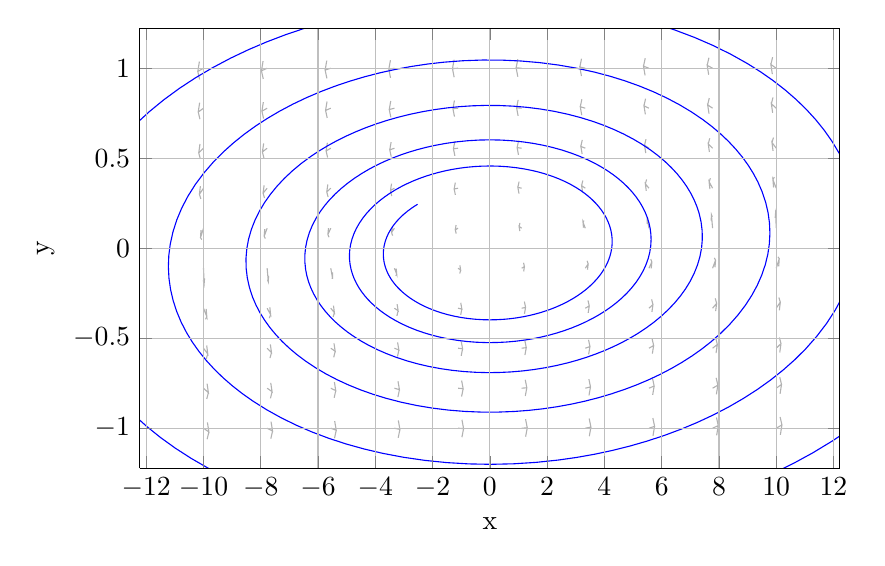
\begin{tikzpicture}

\begin{axis}[%
width=3.5in,
height=2.2in,
at={(0.866319in,1.696914in)},
scale only axis,
unbounded coords=jump,
separate axis lines,
every outer x axis line/.append style={black},
every x tick label/.append style={font=\color{black}},
xmin=-12.2222222222222,
xmax=12.2222222222222,
xlabel={x},
xmajorgrids,
every outer y axis line/.append style={black},
every y tick label/.append style={font=\color{black}},
ymin=-1.22222222222222,
ymax=1.22222222222222,
ylabel={y},
ymajorgrids,
every outer z axis line/.append style={black},
every z tick label/.append style={font=\color{black}},
zmin=-1,
zmax=1,
view={0}{90}
]
\addplot [color=white!70!black,solid,forget plot]
  table[row sep=crcr]{%
-10	-1\\
-9.81241194585928	-1.02056435585844\\
-9.86354727313689	-0.967498035565731\\
-9.81241194585928	-1.02056435585844\\
-9.87382945106611	-1.06129206263609\\
nan	0\\
-10	-0.777777777777778\\
-9.82958536756474	-0.802476346039514\\
-9.87453511522989	-0.752463117452179\\
-9.82958536756474	-0.802476346039514\\
-9.88688439936075	-0.837670433669807\\
nan	0\\
-10	-0.555555555555556\\
-9.85148358196474	-0.587306416934181\\
-9.88810079203066	-0.540652054011778\\
-9.85148358196474	-0.587306416934181\\
-9.90397622271997	-0.614910263029409\\
nan	0\\
-10	-0.333333333333333\\
-9.88446219903126	-0.380389184936132\\
-9.90735957642118	-0.337387979213108\\
-9.88446219903126	-0.380389184936132\\
-9.93088750222258	-0.395156879697477\\
nan	0\\
-10	-0.111111111111111\\
-9.97935536744191	-0.199672451922752\\
-9.96340842200643	-0.167942891539737\\
-9.97935536744191	-0.199672451922752\\
-10.0076890924122	-0.178265207818783\\
nan	0\\
-10	0.111111111111111\\
-10.1051566362561	0.0582449661940668\\
-10.06039310915	0.0478156506051543\\
-10.1051566362561	0.0582449661940668\\
-10.0868261816085	0.100393968733206\\
nan	0\\
-10	0.333333333333333\\
-10.1429235188413	0.299395502359456\\
-10.0915620054455	0.273845971941289\\
-10.1429235188413	0.299395502359456\\
-10.1085309209324	0.34530773136195\\
nan	0\\
-10	0.555555555555555\\
-10.1663153217761	0.529704325960978\\
-10.1099579178447	0.495880864395318\\
-10.1663153217761	0.529704325960978\\
-10.1228835326419	0.579038525283385\\
nan	0\\
-10	0.777777777777778\\
-10.1842555048727	0.756490782015734\\
-10.1236571044704	0.716813004526161\\
-10.1842555048727	0.756490782015734\\
-10.1343006023514	0.808940756962533\\
nan	0\\
-10	1\\
-10.1991602309428	0.981691466175508\\
-10.1348350282039	0.937393968587151\\
-10.1991602309428	0.981691466175508\\
-10.1439892951161	1.03697408405856\\
nan	0\\
-7.77777777777778	-1\\
-7.58854648285336	-1.01579673079962\\
-7.64136668863078	-0.963749887828626\\
-7.58854648285336	-1.01579673079962\\
-7.64926505403059	-1.05836553529084\\
nan	0\\
-7.77777777777778	-0.777777777777778\\
-7.6052640385214	-0.796689610627632\\
-7.65229020208585	-0.747887625958583\\
-7.6052640385214	-0.796689610627632\\
-7.66174611851078	-0.834144495586769\\
nan	0\\
-7.77777777777778	-0.555555555555556\\
-7.62624106257134	-0.57974393076523\\
-7.66565498333085	-0.534603239400719\\
-7.62624106257134	-0.57974393076523\\
-7.67774917093569	-0.610371597003936\\
nan	0\\
-7.77777777777778	-0.333333333333333\\
-7.65642428325531	-0.368944738617867\\
-7.68392748029092	-0.32792294340189\\
-7.65642428325531	-0.368944738617867\\
-7.70173318293318	-0.388599690663124\\
nan	0\\
-7.77777777777778	-0.111111111111111\\
-7.73599401236168	-0.187002745234794\\
-7.72955623345559	-0.153789313643665\\
-7.73599401236168	-0.187002745234794\\
-7.76750205051743	-0.174681196351713\\
nan	0\\
-7.77777777777778	0.111111111111111\\
-7.88119146430226	0.0662767369211356\\
-7.83895876479742	0.0538736275470088\\
-7.88119146430226	0.0662767369211356\\
-7.86137595189241	0.105580470809248\\
nan	0\\
-7.77777777777778	0.333333333333333\\
-7.91930735036248	0.305924850843073\\
-7.86999635796451	0.278765002443974\\
-7.91930735036248	0.305924850843073\\
-7.88370059920964	0.349529788736328\\
nan	0\\
-7.77777777777778	0.555555555555555\\
-7.94285876749928	0.534974090659561\\
-7.88818910435883	0.499878282697984\\
-7.94285876749928	0.534974090659561\\
-7.89847983680683	0.582418777558734\\
nan	0\\
-7.77777777777778	0.777777777777778\\
-7.96093376981838	0.760940492243617\\
-7.90177765082266	0.720202679893716\\
-7.96093376981838	0.760940492243617\\
-7.91019629358974	0.811780675914015\\
nan	0\\
-7.77777777777778	1\\
-7.97594664526146	0.985572129132925\\
-7.91288901729959	0.940358273522127\\
-7.97594664526146	0.985572129132925\\
-7.92010295273312	1.03944270726397\\
nan	0\\
-5.55555555555556	-1\\
-5.36478754435193	-1.01114168970936\\
-5.41923252528567	-0.960107179995643\\
-5.36478754435193	-1.01114168970936\\
-5.42480337014035	-1.05549118559746\\
nan	0\\
-5.55555555555556	-0.777777777777778\\
-5.38111717280357	-0.791071359758572\\
-5.43012529213397	-0.743473689476337\\
-5.38111717280357	-0.791071359758572\\
-5.43677208312436	-0.830692880852331\\
nan	0\\
-5.55555555555556	-0.555555555555556\\
-5.40134491418156	-0.572460909795196\\
-5.44338176803385	-0.528836643179804\\
-5.40134491418156	-0.572460909795196\\
-5.45183444515367	-0.605941963866804\\
nan	0\\
-5.55555555555556	-0.333333333333333\\
-5.42940822002481	-0.357961864284279\\
-5.4610952879463	-0.319036471116309\\
-5.42940822002481	-0.357961864284279\\
-5.47340955342177	-0.382110138881682\\
nan	0\\
-5.55555555555556	-0.111111111111111\\
-5.49219165581084	-0.167585175054708\\
-5.49708230974836	-0.13480198093545\\
-5.49219165581084	-0.167585175054708\\
-5.52531934172015	-0.166483930807808\\
nan	0\\
-5.55555555555556	0.111111111111111\\
-5.65702691981853	0.0758535140774167\\
-5.61777111128121	0.0610629521217819\\
-5.65702691981853	0.0758535140774167\\
-5.63539990979806	0.111798634253268\\
nan	0\\
-5.55555555555556	0.333333333333333\\
-5.69549479662779	0.312987412851764\\
-5.64842654418572	0.284106378728178\\
-5.69549479662779	0.312987412851764\\
-5.65859950442651	0.354075999264293\\
nan	0\\
-5.55555555555556	0.555555555555555\\
-5.71927934431476	0.540504646495139\\
-5.6663994804219	0.504088972023462\\
-5.71927934431476	0.540504646495139\\
-5.67392493495211	0.585950866403066\\
nan	0\\
-5.55555555555556	0.777777777777778\\
-5.73752955813875	0.76554669815799\\
-5.67987958745885	0.723722521398127\\
-5.73752955813875	0.76554669815799\\
-5.68599512726874	0.814709522689726\\
nan	0\\
-5.55555555555556	1\\
-5.75267374583829	0.989558311776526\\
-5.6909278666976	0.943411270672884\\
-5.75267374583829	0.989558311776526\\
-5.69614871080934	1.04197036581425\\
nan	0\\
-3.33333333333333	-1\\
-3.14112720121187	-1.00660003200747\\
-3.19713903284644	-0.956568489374861\\
-3.14112720121187	-1.00660003200747\\
-3.20043904885017	-1.05267155543559\\
nan	0\\
-3.33333333333333	-0.777777777777778\\
-3.15712878001146	-0.785624668790538\\
-3.20802842325483	-0.739219463156243\\
-3.15712878001146	-0.785624668790538\\
-3.21195186876122	-0.827321739817177\\
nan	0\\
-3.33333333333333	-0.555555555555556\\
-3.17675451149172	-0.565472721149544\\
-3.22124886664571	-0.523352866010944\\
-3.17675451149172	-0.565472721149544\\
-3.2262074494427	-0.60164227693175\\
nan	0\\
-3.33333333333333	-0.333333333333333\\
-3.20326704106137	-0.347591861317543\\
-3.23872229674691	-0.310797729854289\\
-3.20326704106137	-0.347591861317543\\
-3.24585156073901	-0.375830875990272\\
nan	0\\
-3.33333333333333	-0.111111111111111\\
-3.25322389641798	-0.143737816344082\\
-3.26910005118434	-0.113922445545352\\
-3.25322389641798	-0.143737816344082\\
-3.28541340380083	-0.153977164003029\\
nan	0\\
-3.33333333333333	0.111111111111111\\
-3.43243096649183	0.0875799333783673\\
-3.39681888211109	0.0698648784085666\\
-3.43243096649183	0.0875799333783673\\
-3.40858447097747	0.119413694987814\\
nan	0\\
-3.33333333333333	0.333333333333333\\
-3.47142332485981	0.320638904989292\\
-3.42682272031586	0.289924735610884\\
-3.47142332485981	0.320638904989292\\
-3.43316993448788	0.358969731374125\\
nan	0\\
-3.33333333333333	0.555555555555555\\
-3.49555527909082	0.546309329973755\\
-3.44457713896812	0.508527711208924\\
-3.49555527909082	0.546309329973755\\
-3.44920025175902	0.589638684087667\\
nan	0\\
-3.33333333333333	0.777777777777778\\
-3.51403282093641	0.770314352070681\\
-3.45795711822871	0.727378507882042\\
-3.51403282093641	0.770314352070681\\
-3.46168883108226	0.817728251683579\\
nan	0\\
-3.33333333333333	1\\
-3.52933604019161	0.99365235096644\\
-3.46894831587574	0.946555968961938\\
-3.52933604019161	0.99365235096644\\
-3.47212214039252	1.04455732239108\\
nan	0\\
-1.11111111111111	-1\\
-0.917557876910838	-1.00217177839591\\
-0.975080902571942	-0.953131936327069\\
-0.917557876910838	-1.00217177839591\\
-0.976166791769897	-1.04990855342721\\
nan	0\\
-1.11111111111111	-0.777777777777778\\
-0.933283653772106	-0.78035043854192\\
-0.985988725782772	-0.735121775977926\\
-0.933283653772106	-0.78035043854192\\
-0.987275056164843	-0.824035504647428\\
nan	0\\
-1.11111111111111	-0.555555555555556\\
-0.952431041938794	-0.558785881461918\\
-0.999227481213899	-0.51814676639693\\
-0.952431041938794	-0.558785881461918\\
-1.00084264416708	-0.597486800983088\\
nan	0\\
-1.11111111111111	-0.333333333333333\\
-0.977842822405366	-0.337909539936786\\
-1.01667925736623	-0.303219605779314\\
-0.977842822405366	-0.337909539936786\\
-1.01896736066795	-0.369853750132186\\
nan	0\\
-1.11111111111111	-0.111111111111111\\
-1.02092818095136	-0.120997422244607\\
-1.04551148221591	-0.0954857963646205\\
-1.02092818095136	-0.120997422244607\\
-1.05045463778266	-0.140577261444496\\
nan	0\\
-1.11111111111111	0.111111111111111\\
-1.20685736361098	0.102309286097334\\
-1.17593303160757	0.0810132704764999\\
-1.20685736361098	0.102309286097334\\
-1.18033394411446	0.128886396726434\\
nan	0\\
-1.11111111111111	0.333333333333333\\
-1.24701179771454	0.328932119310293\\
-1.20514128822775	0.296277311866348\\
-1.24701179771454	0.328932119310293\\
-1.20734189523927	0.364227655168063\\
nan	0\\
-1.11111111111111	0.555555555555555\\
-1.27166140789588	0.55239996184541\\
-1.22270742043291	0.513209065762261\\
-1.27166140789588	0.55239996184541\\
-1.22428521728799	0.593484214154647\\
nan	0\\
-1.11111111111111	0.777777777777778\\
-1.29043246978954	0.775247777514248\\
-1.23600356212013	0.731176437923701\\
-1.29043246978954	0.775247777514248\\
-1.23726856225189	0.820837117262913\\
nan	0\\
-1.11111111111111	1\\
-1.30592761362348	0.997856285321944\\
-1.24694673420026	0.949795274097268\\
-1.30592761362348	0.997856285321944\\
-1.24801859153928	1.04720352535345\\
nan	0\\
1.11111111111111	-1\\
1.30592761362348	-0.997856285321944\\
1.24694673420026	-0.949795274097268\\
1.30592761362348	-0.997856285321944\\
1.24801859153928	-1.04720352535345\\
nan	0\\
1.11111111111111	-0.777777777777778\\
1.29043246978954	-0.775247777514249\\
1.23600356212013	-0.731176437923701\\
1.29043246978954	-0.775247777514249\\
1.23726856225189	-0.820837117262914\\
nan	0\\
1.11111111111111	-0.555555555555556\\
1.27166140789588	-0.55239996184541\\
1.22270742043291	-0.513209065762261\\
1.27166140789588	-0.55239996184541\\
1.22428521728799	-0.593484214154647\\
nan	0\\
1.11111111111111	-0.333333333333333\\
1.24701179771454	-0.328932119310293\\
1.20514128822775	-0.296277311866348\\
1.24701179771454	-0.328932119310293\\
1.20734189523927	-0.364227655168063\\
nan	0\\
1.11111111111111	-0.111111111111111\\
1.20685736361098	-0.102309286097334\\
1.17593303160757	-0.0810132704764999\\
1.20685736361098	-0.102309286097334\\
1.18033394411446	-0.128886396726434\\
nan	0\\
1.11111111111111	0.111111111111111\\
1.02092818095136	0.120997422244607\\
1.04551148221591	0.0954857963646205\\
1.02092818095136	0.120997422244607\\
1.05045463778266	0.140577261444496\\
nan	0\\
1.11111111111111	0.333333333333333\\
0.977842822405366	0.337909539936786\\
1.01667925736623	0.303219605779314\\
0.977842822405366	0.337909539936786\\
1.01896736066795	0.369853750132186\\
nan	0\\
1.11111111111111	0.555555555555555\\
0.952431041938794	0.558785881461917\\
0.999227481213899	0.51814676639693\\
0.952431041938794	0.558785881461917\\
1.00084264416708	0.597486800983088\\
nan	0\\
1.11111111111111	0.777777777777778\\
0.933283653772106	0.780350438541919\\
0.985988725782772	0.735121775977926\\
0.933283653772106	0.780350438541919\\
0.987275056164843	0.824035504647428\\
nan	0\\
1.11111111111111	1\\
0.917557876910838	1.00217177839591\\
0.975080902571942	0.953131936327069\\
0.917557876910838	1.00217177839591\\
0.976166791769897	1.04990855342721\\
nan	0\\
3.33333333333333	-1\\
3.52933604019161	-0.99365235096644\\
3.46894831587574	-0.946555968961938\\
3.52933604019161	-0.99365235096644\\
3.47212214039252	-1.04455732239108\\
nan	0\\
3.33333333333333	-0.777777777777778\\
3.51403282093641	-0.770314352070682\\
3.45795711822871	-0.727378507882042\\
3.51403282093641	-0.770314352070682\\
3.46168883108226	-0.817728251683579\\
nan	0\\
3.33333333333333	-0.555555555555556\\
3.49555527909082	-0.546309329973756\\
3.44457713896812	-0.508527711208924\\
3.49555527909082	-0.546309329973756\\
3.44920025175902	-0.589638684087667\\
nan	0\\
3.33333333333333	-0.333333333333333\\
3.47142332485981	-0.320638904989292\\
3.42682272031586	-0.289924735610884\\
3.47142332485981	-0.320638904989292\\
3.43316993448788	-0.358969731374125\\
nan	0\\
3.33333333333333	-0.111111111111111\\
3.43243096649183	-0.0875799333783673\\
3.39681888211109	-0.0698648784085666\\
3.43243096649183	-0.0875799333783673\\
3.40858447097747	-0.119413694987814\\
nan	0\\
3.33333333333333	0.111111111111111\\
3.25322389641798	0.143737816344082\\
3.26910005118434	0.113922445545352\\
3.25322389641798	0.143737816344082\\
3.28541340380083	0.153977164003029\\
nan	0\\
3.33333333333333	0.333333333333333\\
3.20326704106137	0.347591861317543\\
3.23872229674691	0.310797729854289\\
3.20326704106137	0.347591861317543\\
3.24585156073901	0.375830875990272\\
nan	0\\
3.33333333333333	0.555555555555555\\
3.17675451149172	0.565472721149543\\
3.22124886664571	0.523352866010944\\
3.17675451149172	0.565472721149543\\
3.2262074494427	0.60164227693175\\
nan	0\\
3.33333333333333	0.777777777777778\\
3.15712878001147	0.785624668790538\\
3.20802842325484	0.739219463156243\\
3.15712878001147	0.785624668790538\\
3.21195186876122	0.827321739817177\\
nan	0\\
3.33333333333333	1\\
3.14112720121187	1.00660003200747\\
3.19713903284644	0.956568489374861\\
3.14112720121187	1.00660003200747\\
3.20043904885018	1.05267155543559\\
nan	0\\
5.55555555555556	-1\\
5.75267374583829	-0.989558311776526\\
5.6909278666976	-0.943411270672884\\
5.75267374583829	-0.989558311776526\\
5.69614871080934	-1.04197036581425\\
nan	0\\
5.55555555555556	-0.777777777777778\\
5.73752955813876	-0.76554669815799\\
5.67987958745885	-0.723722521398127\\
5.73752955813876	-0.76554669815799\\
5.68599512726874	-0.814709522689726\\
nan	0\\
5.55555555555556	-0.555555555555556\\
5.71927934431477	-0.540504646495139\\
5.6663994804219	-0.504088972023462\\
5.71927934431477	-0.540504646495139\\
5.67392493495211	-0.585950866403066\\
nan	0\\
5.55555555555556	-0.333333333333333\\
5.69549479662779	-0.312987412851765\\
5.64842654418573	-0.284106378728178\\
5.69549479662779	-0.312987412851765\\
5.65859950442651	-0.354075999264293\\
nan	0\\
5.55555555555556	-0.111111111111111\\
5.65702691981853	-0.0758535140774167\\
5.61777111128121	-0.0610629521217819\\
5.65702691981853	-0.0758535140774167\\
5.63539990979806	-0.111798634253268\\
nan	0\\
5.55555555555556	0.111111111111111\\
5.49219165581084	0.167585175054708\\
5.49708230974836	0.13480198093545\\
5.49219165581084	0.167585175054708\\
5.52531934172016	0.166483930807808\\
nan	0\\
5.55555555555556	0.333333333333333\\
5.42940822002481	0.357961864284279\\
5.4610952879463	0.319036471116309\\
5.42940822002481	0.357961864284279\\
5.47340955342177	0.382110138881681\\
nan	0\\
5.55555555555556	0.555555555555555\\
5.40134491418156	0.572460909795196\\
5.44338176803385	0.528836643179804\\
5.40134491418156	0.572460909795196\\
5.45183444515367	0.605941963866804\\
nan	0\\
5.55555555555556	0.777777777777778\\
5.38111717280357	0.791071359758572\\
5.43012529213397	0.743473689476337\\
5.38111717280357	0.791071359758572\\
5.43677208312436	0.830692880852331\\
nan	0\\
5.55555555555556	1\\
5.36478754435193	1.01114168970936\\
5.41923252528568	0.960107179995643\\
5.36478754435193	1.01114168970936\\
5.42480337014036	1.05549118559746\\
nan	0\\
7.77777777777778	-1\\
7.97594664526146	-0.985572129132925\\
7.91288901729959	-0.940358273522127\\
7.97594664526146	-0.985572129132925\\
7.92010295273312	-1.03944270726397\\
nan	0\\
7.77777777777778	-0.777777777777778\\
7.96093376981838	-0.760940492243617\\
7.90177765082266	-0.720202679893716\\
7.96093376981838	-0.760940492243617\\
7.91019629358974	-0.811780675914015\\
nan	0\\
7.77777777777778	-0.555555555555556\\
7.94285876749928	-0.534974090659561\\
7.88818910435883	-0.499878282697984\\
7.94285876749928	-0.534974090659561\\
7.89847983680683	-0.582418777558735\\
nan	0\\
7.77777777777778	-0.333333333333333\\
7.91930735036249	-0.305924850843073\\
7.86999635796451	-0.278765002443974\\
7.91930735036249	-0.305924850843073\\
7.88370059920964	-0.349529788736328\\
nan	0\\
7.77777777777778	-0.111111111111111\\
7.88119146430226	-0.0662767369211356\\
7.83895876479742	-0.0538736275470088\\
7.88119146430226	-0.0662767369211356\\
7.86137595189241	-0.105580470809248\\
nan	0\\
7.77777777777778	0.111111111111111\\
7.73599401236168	0.187002745234794\\
7.72955623345559	0.153789313643665\\
7.73599401236168	0.187002745234794\\
7.76750205051743	0.174681196351713\\
nan	0\\
7.77777777777778	0.333333333333333\\
7.65642428325531	0.368944738617867\\
7.68392748029092	0.32792294340189\\
7.65642428325531	0.368944738617867\\
7.70173318293319	0.388599690663124\\
nan	0\\
7.77777777777778	0.555555555555555\\
7.62624106257134	0.579743930765229\\
7.66565498333086	0.534603239400719\\
7.62624106257134	0.579743930765229\\
7.67774917093569	0.610371597003936\\
nan	0\\
7.77777777777778	0.777777777777778\\
7.60526403852141	0.796689610627632\\
7.65229020208585	0.747887625958582\\
7.60526403852141	0.796689610627632\\
7.66174611851078	0.834144495586769\\
nan	0\\
7.77777777777778	1\\
7.58854648285336	1.01579673079962\\
7.64136668863078	0.963749887828626\\
7.58854648285336	1.01579673079962\\
7.64926505403059	1.05836553529084\\
nan	0\\
10	-1\\
10.1991602309428	-0.981691466175508\\
10.1348350282039	-0.937393968587151\\
10.1991602309428	-0.981691466175508\\
10.1439892951161	-1.03697408405856\\
nan	0\\
10	-0.777777777777778\\
10.1842555048727	-0.756490782015735\\
10.1236571044704	-0.716813004526161\\
10.1842555048727	-0.756490782015735\\
10.1343006023514	-0.808940756962534\\
nan	0\\
10	-0.555555555555556\\
10.1663153217761	-0.529704325960978\\
10.1099579178447	-0.495880864395318\\
10.1663153217761	-0.529704325960978\\
10.1228835326419	-0.579038525283385\\
nan	0\\
10	-0.333333333333333\\
10.1429235188413	-0.299395502359456\\
10.0915620054455	-0.273845971941289\\
10.1429235188413	-0.299395502359456\\
10.1085309209324	-0.34530773136195\\
nan	0\\
10	-0.111111111111111\\
10.1051566362561	-0.0582449661940668\\
10.06039310915	-0.0478156506051543\\
10.1051566362561	-0.0582449661940668\\
10.0868261816085	-0.100393968733206\\
nan	0\\
10	0.111111111111111\\
9.97935536744191	0.199672451922752\\
9.96340842200643	0.167942891539737\\
9.97935536744191	0.199672451922752\\
10.0076890924122	0.178265207818783\\
nan	0\\
10	0.333333333333333\\
9.88446219903126	0.380389184936132\\
9.90735957642118	0.337387979213108\\
9.88446219903126	0.380389184936132\\
9.93088750222258	0.395156879697477\\
nan	0\\
10	0.555555555555555\\
9.85148358196474	0.587306416934181\\
9.88810079203066	0.540652054011777\\
9.85148358196474	0.587306416934181\\
9.90397622271997	0.614910263029409\\
nan	0\\
10	0.777777777777778\\
9.82958536756474	0.802476346039514\\
9.87453511522989	0.752463117452179\\
9.82958536756474	0.802476346039514\\
9.88688439936075	0.837670433669807\\
nan	0\\
10	1\\
9.81241194585928	1.02056435585844\\
9.86354727313689	0.967498035565731\\
9.81241194585928	1.02056435585844\\
9.87382945106611	1.06129206263609\\
nan	0\\
};
\addplot3 [color=blue,solid]
 table[row sep=crcr] {%
-2.52463885513703	0.243956531381681	0\\
-2.54953737148386	0.241573134930288	0.00093941572513655\\
-2.57423134515417	0.239166444273283	0.0018788314502731\\
-2.59871842594613	0.236736652744317	0.00281824717540965\\
-2.62299628079593	0.234283955824116	0.0037576629005462\\
-2.64706259377769	0.231808551140481	0.00469707862568275\\
-2.67091506610354	0.229310638468288	0.0056364943508193\\
-2.69455141612358	0.226790419729493	0.00657591007595585\\
-2.71796937932587	0.224248098993123	0.0075153258010924\\
-2.87093750186743	0.206430280681934	0.0138892881847653\\
-3.01308353242483	0.187671510045082	0.0202632505684381\\
-3.14374765124357	0.168043579318806	0.026637212952111\\
-3.26232466213577	0.147621573462762	0.0330111753357839\\
-3.36826399248022	0.126483870160022	0.0393851377194568\\
-3.46106969322239	0.104712139817074	0.0457591001031296\\
-3.54030043887437	0.0823913455638228	0.0521330624868025\\
-3.60556952751492	0.0596097432535889	0.0585070248704754\\
-3.65674854854113	0.0363468895394741	0.0649109798562709\\
-3.69319267624266	0.0128026281744376	0.0713149348420665\\
-3.71465353409658	-0.0109262044812335	0.077718889827862\\
-3.7209504564399	-0.0347426366653714	0.0841228448136576\\
-3.71197048846954	-0.058549561213928	0.0905267997994531\\
-3.68766838624232	-0.0822497355609748	0.0969307547852487\\
-3.64806661667503	-0.105745781738703	0.103334709771044\\
-3.59325535754434	-0.128940186377423	0.10973866475684\\
-3.53749851312201	-0.14753326109541	0.11495217130921\\
-3.47185230948046	-0.165810243656967	0.12016567786158\\
-3.39644856418335	-0.183719105734031	0.12537918441395\\
-3.31144648215976	-0.20120908967568	0.13059269096632\\
-3.21703265570418	-0.218230708508127	0.13580619751869\\
-3.11342106447648	-0.234735745934728	0.14101970407106\\
-3.00085307550193	-0.250677256335975	0.14623321062343\\
-2.8795974431712	-0.266009564769501	0.1514467171758\\
-2.73496906640253	-0.282284423132991	0.157241947558176\\
-2.5803964009829	-0.297692900951248	0.163037177940551\\
-2.41635155660908	-0.312177355604101	0.168832408322927\\
-2.24333786526468	-0.325683759822201	0.174627638705302\\
-2.06188988122023	-0.338161701687018	0.180422869087678\\
-1.87257338103308	-0.349564384630844	0.186218099470053\\
-1.6759853635475	-0.359848627436792	0.192013329852428\\
-1.47275404989459	-0.368974864238796	0.197808560234804\\
-1.24026992139891	-0.377702432745986	0.204238510846364\\
-1.00132286913168	-0.384915162046602	0.210668461457923\\
-0.756880311784414	-0.390572688852038	0.217098412069483\\
-0.507927242639707	-0.39464184138227	0.223528362681043\\
-0.255466229571245	-0.397096639365854	0.229958313292602\\
-0.000517415043803648	-0.397918294039927	0.236388263904162\\
0.255881483886752	-0.397095208150209	0.242818214515722\\
0.512675175573474	-0.394622975951	0.249248165127282\\
0.728051775887023	-0.391270089216833	0.254652781745618\\
0.942326705630462	-0.386756187228877	0.260057398363955\\
1.15485799175283	-0.381088613766554	0.265462014982292\\
1.36501198754741	-0.374278238980948	0.270866631600629\\
1.57216337265174	-0.366339459394804	0.276271248218966\\
1.77569515304762	-0.357290197902528	0.281675864837303\\
1.97499866106106	-0.347151903770187	0.28708048145564\\
2.16947355536236	-0.33594955263551	0.292485098073977\\
2.35623358732023	-0.323868243679008	0.297822949387578\\
2.53714879569578	-0.310805468894792	0.303160800701179\\
2.71166533402786	-0.296794005001333	0.30849865201478\\
2.8792510552048	-0.281869335907071	0.313836503328381\\
3.0393955114644	-0.266069652710418	0.319174354641982\\
3.19160995439394	-0.249435853699758	0.324512205955584\\
3.33542733493016	-0.232011544353442	0.329850057269185\\
3.47040230335928	-0.213843037339796	0.335187908582786\\
3.61416004235552	-0.192090168523607	0.341326815907968\\
3.74505296214502	-0.169493719262271	0.347465723233149\\
3.86249878011785	-0.146135404991408	0.353604630558331\\
3.96597306874113	-0.122099493172007	0.359743537883513\\
4.055009255559	-0.0974728032904351	0.365882445208694\\
4.12919862319264	-0.072344706858429	0.372021352533876\\
4.18819030934024	-0.0468071274131004	0.378160259859057\\
4.23169130677705	-0.0209545405169332	0.384299167184239\\
4.2580712590717	0.00333609511056443	0.390019732919852\\
4.27062401230471	0.0277387196872827	0.395740298655465\\
4.26923027485969	0.0521726547075702	0.401460864391079\\
4.25381984529303	0.0765575417634933	0.407181430126692\\
4.2243716123339	0.100813342544836	0.412901995862305\\
4.18091355488423	0.1248603388391	0.418622561597918\\
4.12352274201875	0.148619132531505	0.424343127333531\\
4.05232533298495	0.172010645604989	0.430063693069144\\
3.9787313005877	0.192140749170099	0.435075523518222\\
3.89479990435716	0.211876457286547	0.440087353967299\\
3.80069580327496	0.231165598145863	0.445099184416376\\
3.69660987515563	0.249957372712364	0.450111014865454\\
3.58275921664664	0.268202354723152	0.455122845314531\\
3.45938714322839	0.285852490688118	0.460134675763608\\
3.32676318921417	0.302861099889936	0.465146506212686\\
3.18518310775021	0.31918287438407	0.470158336661763\\
3.00795439468882	0.337410896808102	0.476042580715478\\
2.81936808959254	0.354563369136315	0.481926824769194\\
2.62002360626585	0.370573526666975	0.487811068822909\\
2.41055659059686	0.385379195936704	0.493695312876624\\
2.19163892055738	0.398922794720484	0.49957955693034\\
1.96397870620289	0.41115133203165	0.505463800984055\\
1.72832028967254	0.422016408121895	0.51134804503777\\
1.48544424518916	0.431474214481271	0.517232289091486\\
1.21036192340659	0.440221183032222	0.523717366640754\\
0.928597675959549	0.447163479368953	0.530202444190022\\
0.641318758376293	0.45225934008511	0.536687521739291\\
0.349708955064771	0.455475651364104	0.543172599288559\\
0.0549685793126407	0.456787948979118	0.549657676837828\\
-0.241685526712736	0.456180418293104	0.556142754387096\\
-0.539019991964293	0.453645894258782	0.562627831936365\\
-0.835784916515264	0.449185861418642	0.569112909485633\\
-1.0801310939543	0.444042666077613	0.574481366189135\\
-1.3225179323629	0.437592974688615	0.579849822892637\\
-1.56222532421052	0.429848916854006	0.585218279596139\\
-1.79854456138531	0.420826506262126	0.590586736299641\\
-2.03077833519408	0.410545640687297	0.595955193003143\\
-2.25824073636236	0.399030101989818	0.601323649706645\\
-2.48025725503432	0.386307556115973	0.606692106410146\\
-2.69616478077284	0.372409553098023	0.612060563113648\\
-2.90909737484152	0.357083617291038	0.617527736543755\\
-3.11434774240454	0.340614312495133	0.622994909973862\\
-3.31125140418673	0.323045641339808	0.628462083403968\\
-3.49917340591627	0.304424873187658	0.633929256834075\\
-3.6775083183247	0.284802544134369	0.639396430264182\\
-3.8456802371469	0.264232457008719	0.644863603694289\\
-4.00314278312111	0.24277168137258	0.650330777124395\\
-4.1493791019889	0.220480553520914	0.655797950554502\\
-4.30138347266504	0.194209297836297	0.662013312356874\\
-4.43757638684455	0.167041697254854	0.668228674159246\\
-4.55732215685077	0.139079292614893	0.674444035961618\\
-4.66005724091033	0.110426249090555	0.68065939776399\\
-4.74529024315323	0.0811893561918218	0.686874759566362\\
-4.81260191361277	0.0514780277645118	0.693090121368734\\
-4.86164514822559	0.0214043019902807	0.699305483171106\\
-4.89214498883165	-0.00891715861337908	0.705520844973478\\
-4.90345962977691	-0.0356155959869364	0.710970421242432\\
-4.90023965023054	-0.0623366841666692	0.716419997511386\\
-4.88241814227239	-0.0889998586991246	0.72186957378034\\
-4.84997435484199	-0.115525114799782	0.727319150049294\\
-4.8029336937386	-0.141833007353052	0.732768726318248\\
-4.74136772162114	-0.167844650912278	0.738218302587202\\
-4.66539415800825	-0.193481719699734	0.743667878856156\\
-4.57517687927826	-0.218666447606629	0.74911745512511\\
-4.48002780884107	-0.241313713763144	0.754118264957009\\
-4.37323505382051	-0.263456436462847	0.759119074788909\\
-4.25501424674027	-0.285036042603881	0.764119884620808\\
-4.12561022761644	-0.305995655072633	0.769120694452708\\
-3.98529704395749	-0.326280092743741	0.774121504284607\\
-3.83437795076429	-0.345835870480088	0.779122314116507\\
-3.67318541053011	-0.364611199132803	0.784123123948406\\
-3.50208109324059	-0.382555985541264	0.789123933780306\\
-3.2857589370373	-0.40279067879689	0.795083563795009\\
-3.05660320166021	-0.421698802355246	0.801043193809713\\
-2.81536781006231	-0.439204064421199	0.807002823824416\\
-2.56284797294821	-0.455235932834348	0.81296245383912\\
-2.29988018877408	-0.469729635069017	0.818922083853823\\
-2.02734224374768	-0.482626158234261	0.824881713868527\\
-1.74615321182836	-0.493872249073861	0.83084134388323\\
-1.45727345472705	-0.503420413966331	0.836800973897934\\
-1.13243096622625	-0.511898489576752	0.843343768968266\\
-0.800846502565246	-0.518230196439062	0.849886564038599\\
-0.463926513581075	-0.522373472657226	0.856429359108931\\
-0.123091691784856	-0.524296647442224	0.862972154179264\\
0.220223027638204	-0.523978441112045	0.869514949249596\\
0.564568466828807	-0.521407965091686	0.876057744319928\\
0.908481205253567	-0.516584721913158	0.882600539390261\\
1.25048357970502	-0.509518605215481	0.889143334460593\\
1.52685136182108	-0.502110892701279	0.894477071976976\\
1.80017017740532	-0.493237207586073	0.89981080949336\\
2.0696342615021	-0.482915674745765	0.905144547009743\\
2.33445299128273	-0.471168685433431	0.910478284526126\\
2.5938508860454	-0.458022897279325	0.91581202204251\\
2.84706760721524	-0.443509234290877	0.921145759558893\\
3.09335795834426	-0.427662886852689	0.926479497075276\\
3.33199188511143	-0.410523311726544	0.931813234591659\\
3.57296731548468	-0.391230423439519	0.937400006255398\\
3.80396052730072	-0.370618832041845	0.942986777919136\\
4.0241836855056	-0.348746821402461	0.948573549582874\\
4.23288851141038	-0.325676551678942	0.954160321246612\\
4.42936628269115	-0.301474059317501	0.959747092910351\\
4.61294783338905	-0.276209257052983	0.965333864574089\\
4.78300355391024	-0.249955933908872	0.970920636237827\\
4.93894339102594	-0.222791755197286	0.976507407901565\\
5.09695909764897	-0.191214261779277	0.982798072832153\\
5.2356469506793	-0.158702605364944	0.989088737762741\\
5.35432398752309	-0.125382248726769	0.995379402693329\\
5.45239668617473	-0.0913812425908319	1.00167006762392\\
5.52936096521684	-0.0568302256368078	1.0079607325545\\
5.58480218382025	-0.0218624244979693	1.01425139748509\\
5.61839514174403	0.0133863462388142	1.02054206241568\\
5.62990407933544	0.0487776840330781	1.02683272734627\\
5.62203885895981	0.0791744564792287	1.03223416376666\\
5.59770332674167	0.10948492986247	1.03763560018704\\
5.55688376384794	0.139618763786658	1.04303703660743\\
5.49961731935771	0.169486576154884	1.04843847302782\\
5.42599201026228	0.198999943169474	1.05383990944821\\
5.33614672146511	0.228071399331993	1.0592413458686\\
5.23027120578187	0.256614437443239	1.06464278228899\\
5.10860608394038	0.284543508603249	1.07004421870937\\
4.97633356131725	0.310863992906032	1.0752625459558\\
4.82987567839244	0.336457776915644	1.08048087320223\\
4.66956654150022	0.361250448835276	1.08569920044866\\
4.49577859503672	0.385170205660132	1.09091752769508\\
4.30892262145996	0.408147853177434	1.09613585494151\\
4.10944774128986	0.43011680596642	1.10135418218794\\
3.89784141310818	0.451013087398344	1.10657250943437\\
3.6746294335586	0.470775329636476	1.1117908366808\\
3.40108260051971	0.492262265885678	1.11786162768086\\
3.11350670569581	0.512047037949123	1.12393241868093\\
2.81289795512307	0.530044977352055	1.13000320968099\\
2.50029770423504	0.546178968513058	1.13607400068106\\
2.1767924578627	0.560379448744062	1.14214479168112\\
1.84351387023446	0.572584408250339	1.14821558268119\\
1.50163874497611	0.582739390130504	1.15428637368126\\
1.15238903511087	0.590797490376516	1.16035716468132\\
0.774401234740981	0.597020414278004	1.16681097735645\\
0.391018877244034	0.600787465808141	1.17326479003157\\
0.00383870456758495	0.602066497087122	1.17971860270669\\
-0.385536914574306	0.600836724898174	1.18617241538182\\
-0.775499984701076	0.597088730687549	1.19262622805694\\
-1.16443688356565	0.590824460564531	1.19908004073206\\
-1.55072836215446	0.582057225301431	1.20553385340719\\
-1.93274954468742	0.570811700333588	1.21198766608231\\
-2.23880098516255	0.559875774153527	1.21722994404303\\
-2.54010623989631	0.547347783612344	1.22247222200376\\
-2.83580043306064	0.533254693590891	1.22771449996448\\
-3.12503859556705	0.517627887513325	1.23295677792521\\
-3.40699566506663	0.50050316734712	1.23819905588593\\
-3.68086648595004	0.48192075360306	1.24344133384665\\
-3.94586580934751	0.461925285335244	1.24868361180738\\
-4.20122829312885	0.44056582014108	1.2539258897681\\
-4.46912041172518	0.415655585448098	1.25967044428071\\
-4.7235981794682	0.389244507514765	1.26541499879333\\
-4.9637309276595	0.361412881399265	1.27115955330594\\
-5.18864326647325	0.332245549745374	1.27690410781855\\
-5.3975150849562	0.301831902782459	1.28264866233117\\
-5.58958155102767	0.270265878325481	1.28839321684378\\
-5.76413311147957	0.237645961774991	1.29413777135639\\
-5.92051549197638	0.204075186117134	1.299882325869\\
-6.07250831957859	0.165714183359902	1.30627713805909\\
-6.20048224308383	0.12645675833523	1.31267195024917\\
-6.303746912819	0.0864611352388039	1.31906676243925\\
-6.38172526307845	0.0458876759251402	1.32546157462933\\
-6.43395351212402	0.00489887990758892	1.33185638681941\\
-6.46008116218502	-0.036340615641668	1.3382511990095\\
-6.45987099945826	-0.0776640358916159	1.34464601119958\\
-6.43319909410797	-0.118902468352409	1.35104082338966\\
-6.3906272033124	-0.153150048186647	1.35638059839411\\
-6.32959934844859	-0.187121762939165	1.36172037339856\\
-6.2501974584375	-0.220717763370481	1.36706014840301\\
-6.15255839005245	-0.253839774536682	1.37239992340746\\
-6.03687392791903	-0.286391095789431	1.37773969841192\\
-5.90339078451516	-0.318276600775966	1.38307947341637\\
-5.7524106001711	-0.349402737439093	1.38841924842082\\
-5.5842899430694	-0.379677528017196	1.39375902342527\\
-5.39484430476572	-0.409695163550463	1.39922544894041\\
-5.18833259126714	-0.438631352493332	1.40469187445556\\
-4.96529195461284	-0.466392450380913	1.4101582999707\\
-4.72630923654709	-0.492888968660615	1.41562472548585\\
-4.47202096851926	-0.518035574692146	1.42109115100099\\
-4.20311337168382	-0.54175109174751	1.42655757651614\\
-3.92032235690035	-0.563958499011011	1.43202400203128\\
-3.6244335247335	-0.584584931579251	1.43749042754643\\
-3.27323947734976	-0.606024609299606	1.44370391169096\\
-2.90745082944039	-0.625238112288525	1.4499173958355\\
-2.52841813561522	-0.642135840254608	1.45613087998003\\
-2.13753787772163	-0.65663834524016	1.46234436412456\\
-1.73625246484452	-0.668676331621196	1.4685578482691\\
-1.3260502333063	-0.678190656107438	1.47477133241363\\
-0.908465446666925	-0.685132327742314	1.48098481655816\\
-0.485078295723864	-0.68946250790296	1.48719830070269\\
-0.0823042790979306	-0.691125916687632	1.49305234726862\\
0.322838983398461	-0.690424975978886	1.49890639383454\\
0.728950576029773	-0.68734849164594	1.50476044040046\\
1.13463394379846	-0.681893994450682	1.51061448696638\\
1.53849689244495	-0.674067740047676	1.5164685335323\\
1.93915158844768	-0.663884708984158	1.52232258009822\\
2.33521455902307	-0.651368606700039	1.52817662666414\\
2.72530669212553	-0.636551863527901	1.53403067323006\\
3.05568570915643	-0.621965493416638	1.53907616331742\\
3.37974409875082	-0.605727979124974	1.54412165340477\\
3.69661443656387	-0.587873337944721	1.54916714349213\\
4.00545182470155	-0.568439783073034	1.55421263357949\\
4.30543389172056	-0.547469723612406	1.55925812366684\\
4.59576079262842	-0.525009764570673	1.5643036137542\\
4.87565520888341	-0.501110706861014	1.56934910384156\\
5.14436234839459	-0.475827547301945	1.57439459392892\\
5.44177656662719	-0.444766634101765	1.58026116104664\\
5.72197069084942	-0.412010814855438	1.58612772816436\\
5.98386252380373	-0.377665150115029	1.59199429528208\\
6.22644303097867	-0.34183992843919	1.5978608623998\\
6.44877634060887	-0.304650666393161	1.60372742951752\\
6.64999974367505	-0.266218108548766	1.60959399663524\\
6.82932369390403	-0.226668227484417	1.61546056375296\\
6.9860318077687	-0.186132223785111	1.62132713087068\\
7.13194739077126	-0.140416425258992	1.62780084306816\\
7.24875372667252	-0.0938486153146721	1.63427455526565\\
7.33575866567383	-0.0466226750675951	1.64074826746313\\
7.39240927445341	0.0010659401770956	1.64722197966061\\
7.41829183616633	0.0490202009245581	1.6536956918581\\
7.41313185044453	0.0970415034902513	1.66016940405558\\
7.37679403339684	0.144929669999935	1.66664311625307\\
7.30928231760891	0.192482948389671	1.67311682845055\\
7.23096001557147	0.230989216768199	1.67841189481341\\
7.13196032206585	0.269026831837128	1.68370696117628\\
7.01246000748691	0.306485059062228	1.68900202753914\\
6.8726956951557	0.343255358250338	1.69429709390201\\
6.71296386131948	0.379231383549362	1.69959216026487\\
6.53362083515169	0.414308983448276	1.70488722662773\\
6.33508279875199	0.448386200777122	1.7101822929906\\
6.11782578714619	0.481363272707012	1.71547735935346\\
5.86697312913968	0.515099773697118	1.72110534075919\\
5.59625394206166	0.547369609859529	1.72673332216492\\
5.30643181102717	0.578060714849136	1.73236130357065\\
4.99833057370882	0.607066895048946	1.73798928497638\\
4.67283432033674	0.634287829570081	1.74361726638211\\
4.33088739369865	0.659629070251776	1.74924524778785\\
3.97349438913982	0.683002041661383	1.75487322919358\\
3.60172015456305	0.704324041094369	1.76050121059931\\
3.16870830355461	0.725717612934557	1.7668175621919\\
2.72060632280285	0.744330025211493	1.7731339137845\\
2.25914395195512	0.76006771268084	1.7794502653771\\
1.78609636241945	0.772850039588954	1.78576661696969\\
1.3032841573646	0.782609299672881	1.79208296856229\\
0.812573371720026	0.789290716160358	1.79839932015489\\
0.315875472175895	0.792852441769813	1.80471567174748\\
-0.184852642816931	0.793265558710366	1.81103202334008\\
-0.620397685527848	0.791063521530621	1.81650420954154\\
-1.05618854490361	0.786477623949286	1.821976395743\\
-1.4908995674507	0.779509196725716	1.82744858194445\\
-1.92321480455029	0.770167109374572	1.83292076814591\\
-2.35182801245825	0.758467770165823	1.83839295434737\\
-2.77544265230519	0.744435126124746	1.84386514054882\\
-3.19277189009639	0.728100663031926	1.84933732675028\\
-3.60253859671186	0.709503405423253	1.85480951295174\\
-3.97069740335034	0.690492399221125	1.85982921843037\\
-4.33046523087744	0.669654173747204	1.86484892390901\\
-4.68088230970327	0.647033283435818	1.86986862938765\\
-5.02101721595129	0.622678833292475	1.87488833486628\\
-5.34996687145831	0.59664447889386	1.87990804034492\\
-5.66685654377449	0.568988426387834	1.88492774582356\\
-5.97083984616335	0.539773432493437	1.88994745130219\\
-6.26109873760173	0.509066804500887	1.89496715678083\\
-6.58737753736975	0.470701305130512	1.90093736618176\\
-6.89185643833642	0.430452097139635	1.90690757558269\\
-7.17330004719471	0.388454287764456	1.91287778498361\\
-7.43056779971555	0.344848829155739	1.91884799438454\\
-7.66261396074784	0.29978251837881	1.92481820378547\\
-7.86848762421841	0.25340799741356	1.9307884131864\\
-8.04733271313209	0.20588375315444	1.93675862258732\\
-8.19838797957162	0.157374117410465	1.94272883198825\\
-8.32839419185422	0.10461078108421	1.94911156313784\\
-8.42514137044121	0.0511219312172363	1.95549429428743\\
-8.4880118726577	-0.00287448250690836	1.96187702543702\\
-8.5165404668062	-0.0571598037156272	1.96825975658661\\
-8.51041433216656	-0.111514669347273	1.9746424877362\\
-8.46947305899601	-0.165719009651147	1.9810252188858\\
-8.39370864852913	-0.219552048187502	1.98740795003539\\
-8.28326551297786	-0.272792301827539	1.99379068118498\\
-8.16727856612876	-0.315761280455246	1.99901330727899\\
-8.02843918129436	-0.358065697314853	2.004235933373\\
-7.86701759282634	-0.399585039926258	2.00945855946701\\
-7.68334779370324	-0.440201556102759	2.01468118556103\\
-7.47782753553043	-0.479800253951053	2.01990381165504\\
-7.2509183285401	-0.518268901871232	2.02512643774905\\
-7.00314544159129	-0.555498028556786	2.03034906384306\\
-6.73509790216988	-0.591380922994606	2.03557168993707\\
-6.41770382576029	-0.629162143560262	2.04131459829506\\
-6.07749105013688	-0.665056372723018	2.04705750665304\\
-5.71547364078329	-0.698932441940981	2.05280041501102\\
-5.33273659773053	-0.730666956214703	2.058543323369\\
-4.93043585555696	-0.760144294087184	2.06428623172698\\
-4.5097982833883	-0.787256607643872	2.07002914008496\\
-4.07212168489767	-0.81190382251266	2.07577204844295\\
-3.61877479830549	-0.83399363786389	2.08151495680093\\
-3.09742533284057	-0.855473063250543	2.08790756963223\\
-2.56043944450083	-0.873571541115752	2.09430018246353\\
-2.00995802777812	-0.888191605965933	2.10069279529483\\
-1.44816626644943	-0.8992517300686	2.10708540812613\\
-0.877293633576849	-0.906686323452369	2.11347802095743\\
-0.299613891507601	-0.910445733906954	2.11987063378873\\
0.282554908125965	-0.910496246983171	2.12626324662003\\
0.866850424406395	-0.906820085992938	2.13265585945134\\
1.36218192190706	-0.900779381861014	2.13807618199253\\
1.85587718558672	-0.892058379435891	2.14349650453373\\
2.34645312029365	-0.880669088272393	2.14891682707493\\
2.83244317271144	-0.866631746304842	2.15433714961612\\
3.31239733135896	-0.849974819847056	2.15975747215732\\
3.78488212659037	-0.830735003592351	2.16517779469851\\
4.24848063059511	-0.80895722061354	2.17059811723971\\
4.70179245739797	-0.784694622362931	2.17601843978091\\
5.12914999854503	-0.758920565745572	2.18126085562998\\
5.54436499810676	-0.730937609314474	2.18650327147905\\
5.94621738349823	-0.700812759279218	2.19174568732811\\
6.33353094190753	-0.668618941810985	2.19698810317718\\
6.70517332029577	-0.63443500304255	2.20223051902625\\
7.06005602539708	-0.59834570906829	2.20747293487532\\
7.39713442371858	-0.560441745944176	2.21271535072439\\
7.71540774154045	-0.52081971968778	2.21795776657346\\
8.06001782828526	-0.472806782411799	2.2240428825598\\
8.37658273579564	-0.422781021619633	2.23012799854615\\
8.66373659763812	-0.370919185440678	2.23621311453249\\
8.92023831839865	-0.317404188062106	2.24229823051883\\
9.14497157368264	-0.262425109728872	2.24838334650517\\
9.33694481011493	-0.206177196743708	2.25446846249152\\
9.49529124533981	-0.148861861467127	2.26055357847786\\
9.619268868021	-0.0906866823174207	2.2666386944642\\
9.70645329622627	-0.0333409560601755	2.27257137097833\\
9.75986713283432	0.024423493135505	2.27850404749245\\
9.77912053965396	0.0824018949201975	2.28443672400657\\
9.76395403726019	0.140389868978681	2.29036940052069\\
9.71423850499414	0.198183425029939	2.29630207703481\\
9.62997518096313	0.255578962827154	2.30223475354894\\
9.51129566204065	0.312373272157713	2.30816743006306\\
9.35846190386631	0.368363532843209	2.31410010657718\\
9.20095551934731	0.415452051559984	2.31917318097207\\
9.0190215542187	0.461680423751387	2.32424625536695\\
8.81301715085464	0.506923754264707	2.32931932976184\\
8.58336318600369	0.551060295154759	2.33439240415672\\
8.33054427078875	0.593971445683884	2.33946547855161\\
8.0551087507071	0.63554175232195	2.34453855294649\\
7.7576687056304	0.675658908746349	2.34961162734138\\
7.43889994980468	0.714213755842	2.35468470173626\\
7.04660828704447	0.756513533831438	2.36052278596119\\
6.6282273182079	0.796448522705435	2.36636087018612\\
6.18505977174931	0.83386646118593	2.37219895441106\\
5.7184909503309	0.868625065354876	2.37803703863599\\
5.22998873082275	0.900592028654237	2.38387512286092\\
4.72110356430278	0.929645021885988	2.38971320708585\\
4.19346847605681	0.955671693212117	2.39555129131078\\
3.64879906557848	0.978569668154625	2.40138937553572\\
3.0289610240322	1.00013209317583	2.40784332285879\\
2.39293525662299	1.01764398470027	2.41429727018186\\
1.74332336329521	1.03100421538214	2.42075121750493\\
1.0827692263002	1.04013096064601	2.427205164828\\
0.413959010196292	1.04496169868682	2.43365911215107\\
-0.260378838151203	1.0454532104699	2.44011305947414\\
-0.93747358956999	1.04158157973097	2.44656700679721\\
-1.6145122325808	1.03334219297611	2.45302095412028\\
-2.17689684307492	1.02314129855567	2.45840171485177\\
-2.73564173683773	1.00992419309241	2.46378247558326\\
-3.2890838111643	0.993714115544783	2.46916323631475\\
-3.83558371912983	0.974543350639405	2.47454399704623\\
-4.37352586958964	0.952453228871078	2.47992475777772\\
-4.90131842717919	0.927494126502765	2.48530551850921\\
-5.41739331231404	0.899725465565603	2.49068627924069\\
-5.92020620118992	0.869215713858894	2.49606703997218\\
-6.40959480374461	0.835943884935875	2.50146284574448\\
-6.88262172581133	0.80007507402389	2.50685865151677\\
-7.33780188272023	0.761701905547488	2.51225445728906\\
-7.77371186044875	0.720924282624006	2.51765026306136\\
-8.18898991562157	0.677849387063569	2.52304606883365\\
-8.58233597551064	0.632591679369092	2.52844187460595\\
-8.95251163803514	0.585272898736282	2.53383768037824\\
-9.29834017176155	0.536022063053629	2.53923348615053\\
-9.66266544803018	0.477487153792858	2.54540566436602\\
-9.99210136880628	0.416809696614699	2.55157784258151\\
-10.2851514928621	0.354212355771737	2.557750020797\\
-10.5404772233976	0.28992419057178	2.56392219901249\\
-10.7568978080404	0.224180655377858	2.57009437722798\\
-10.9333903388461	0.157223599608226	2.57626655544347\\
-11.0690897522978	0.0893012677363615	2.58243873365896\\
-11.1632888293064	0.0206682992909623	2.58861091187445\\
-11.2121125710753	-0.041500931331536	2.59416622033823\\
-11.2265095356813	-0.103847236085748	2.59972152880202\\
-11.2062486281477	-0.166175836820932	2.6052768372658\\
-11.151213155704	-0.228292973743479	2.61083214572958\\
-11.0614008277866	-0.29000590541691	2.61638745419337\\
-10.9369237560386	-0.351122908761883	2.62194276265715\\
-10.7780084543096	-0.411453279056186	2.62749807112094\\
-10.5849958386561	-0.470807329934741	2.63305337958472\\
-10.3843631338935	-0.522785463066766	2.63800971777722\\
-10.1572980361086	-0.573704553911172	2.64296605596972\\
-9.90424207774905	-0.623432757063133	2.64792239416223\\
-9.62570218762491	-0.671841773777611	2.65287873235473\\
-9.32225069090842	-0.718806851969361	2.65783507054723\\
-8.99452530913407	-0.764206786212928	2.66279140873973\\
-8.64322916019858	-0.807923917742648	2.66774774693224\\
-8.26913075836094	-0.849844134452648	2.67270408512474\\
-7.79454645117989	-0.897315247828815	2.67861213305705\\
-7.29022181545536	-0.941896570749325	2.68452018098935\\
-6.75777724932292	-0.983412643744195	2.69042822892166\\
-6.19892833653566	-1.02170041228386	2.69633627685396\\
-5.6154858464642	-1.05660922677916	2.70224432478627\\
-5.00935573409671	-1.08800084258136	2.70815237271857\\
-4.38253914003887	-1.11574941998212	2.71406042065088\\
-3.73713239051388	-1.13974152421352	2.71996846858319\\
-3.0081258799778	-1.16167856379716	2.72646853894455\\
-2.26218340808047	-1.17882439507779	2.73296860930591\\
-1.50241489871464	-1.19107321960495	2.73946867966727\\
-0.731970580312717	-1.19834225531587	2.74596875002863\\
0.0459590141531376	-1.2005717365355	2.75246882038999\\
0.828143047171071	-1.1977249139765	2.75896889075135\\
1.61131037668951	-1.18978805473922	2.76546896111272\\
2.39214955611718	-1.17677044231172	2.77196903147408\\
3.03102300881354	-1.16225588244583	2.77732129416272\\
3.66421965053062	-1.14433708516567	2.78267355685137\\
4.2898668569668	-1.12304866153269	2.78802581954001\\
4.90612320576226	-1.09843525731469	2.79337808222866\\
5.51117847649894	-1.07055155298583	2.7987303449173\\
6.10325365070057	-1.03946226372661	2.80408260760595\\
6.68060091183263	-1.0052421394239	2.8094348702946\\
7.24150364530241	-0.967975964670928	2.81478713298324\\
7.79894935274937	-0.926609383044724	2.82028657440474\\
8.33547467252608	-0.882234053344814	2.82578601582624\\
8.84931782503836	-0.834970420667621	2.83128545724774\\
9.33879807175556	-0.784947593617764	2.83678489866924\\
9.80231571521064	-0.732303344308053	2.84228434009074\\
10.2383520990001	-0.677184108359492	2.84778378151224\\
10.6454696077842	-0.619744984901278	2.85328322293375\\
11.0223116672864	-0.560149736570799	2.85878266435525\\
11.4113469440435	-0.490189440778743	2.86501759140895\\
11.75808525432	-0.417933441797551	2.87125251846266\\
12.0608855743963	-0.343654118868716	2.87748744551636\\
12.3183005283069	-0.267630483600682	2.88372237257006\\
12.52907638784	-0.190148179968844	2.88995729962377\\
12.6921530725378	-0.111499484315548	2.89619222667747\\
12.8066641496967	-0.0319833053500922	2.90242715373118\\
12.8719368343667	0.0480948158512762	2.90866208078488\\
12.8882673452644	0.118049496700103	2.91409178612164\\
12.8666093760493	0.187991258852486	2.9195214914584\\
12.8068284568934	0.257710404846056	2.92495119679516\\
12.7089095256758	0.326998904894184	2.93038090213192\\
12.5729569279837	0.395650396885981	2.93581060746868\\
12.3991944171115	0.463460186386292	2.94124031280544\\
12.1879651540615	0.530225246635704	2.9466700181422\\
11.9397317075433	0.595744218550541	2.95209972347896\\
11.675538360385	0.655514944474858	2.95716047739867\\
11.3802084837525	0.713870958774254	2.96222123131839\\
11.0543596199686	0.770653780179413	2.9672819852381\\
10.6986890844395	0.825709769851905	2.97234273915782\\
10.3139739656546	0.878890131384178	2.97740349307753\\
9.90107112518632	0.930050910799561	2.98246424699724\\
9.46091719769077	0.979052996552267	2.98752500091696\\
8.99452859090709	1.02576211952739	2.99258575483667\\
8.41021397365933	1.0778987401622	2.99857436708134\\
7.79258194122756	1.12643869396962	3.004562979326\\
7.14369292254008	1.17118312557787	3.01055159157067\\
6.4657146010001	1.21194887909542	3.01654020381533\\
5.76092191448576	1.24856849811098	3.02252881606\\
5.03169705535015	1.28089022569357	3.02851742830467\\
4.28052947042124	1.30877800439245	3.03450604054933\\
3.51001586100194	1.33211147623713	3.040494652794\\
2.64560797594893	1.35234741859064	3.04706440433253\\
1.76472235764726	1.36685308474415	3.05363415587107\\
0.871136737304051	1.37552592954323	3.06020390740961\\
-0.0313401659863244	1.3782912743625	3.06677365894815\\
-0.938868645242257	1.3751023071056	3.07334341048669\\
-1.8475780055949	1.36594008220519	3.07991316202522\\
-2.75356656428816	1.35081352062297	3.08648291356376\\
-3.65290165067873	1.32975940984967	3.0930526651023\\
-4.37267451067564	1.30843594743067	3.09836580941991\\
-5.08346041826752	1.28331197506441	3.10367895373752\\
-5.78317475324837	1.25444013214131	3.10899209805512\\
-6.46977500721855	1.22188398871667	3.11430524237273\\
-7.14126078358475	1.18571804551059	3.11961838669034\\
-7.79567379756001	1.14602773390805	3.12493153100795\\
-8.4310978761637	1.10290941595881	3.13024467532556\\
-9.04565895822154	1.05647038437753	3.13555781964316\\
-9.67290341495032	1.00369454898733	3.14119529027746\\
-10.2724762533718	0.947459753252776	3.14683276091176\\
-10.8422860336584	0.887928857358942	3.15247023154606\\
-11.3803523216538	0.825274994511738	3.15810770218036\\
-11.8848056888728	0.759681570937893	3.16374517281466\\
-12.3538877125015	0.691342265884955	3.16938264344896\\
-12.7859509753972	0.620461031621297	3.17502011408326\\
-13.1794590660881	0.547252093436108	3.18065758471756\\
-13.5732519747866	0.462632652239153	3.18698133754964\\
-13.9148681940253	0.375685356495249	3.19330509038172\\
-14.2025793610443	0.286750481910354	3.19962884321381\\
-14.4348999835445	0.196174515815817	3.20595259604589\\
-14.610587439688	0.104310157168388	3.21227634887798\\
-14.7286419780975	0.0115163165502062	3.21860010171006\\
-14.7883067178571	-0.0818418838311884	3.22492385454214\\
-14.7890676485115	-0.175393110142866	3.23124760737423\\
-14.7431534399352	-0.254792865048927	3.23662328347769\\
-14.6543382717503	-0.333832210926983	3.24199895958115\\
-14.5226605915265	-0.412277136519469	3.24737463568461\\
-14.3482894692575	-0.489896503036653	3.25275031178808\\
-14.1315245973602	-0.566462044156631	3.25812598789154\\
-13.8727962906755	-0.641748366025334	3.263501663995\\
-13.572665486468	-0.715532947256523	3.26887734009846\\
-13.2318237444257	-0.787596138931791	3.27425301620192\\
-12.8565464707135	-0.856777035662155	3.27955507959187\\
-12.4433028568926	-0.923869104927903	3.28485714298182\\
-11.9930796494393	-0.98867007662925	3.29015920637177\\
-11.5069689433646	-1.05098535602045	3.29546126976172\\
-10.9861681822145	-1.11062802370979	3.30076333315166\\
-10.4319801580691	-1.16741883565961	3.30606539654161\\
-9.84581301154382	-1.22118622318628	3.31136745993156\\
-9.22918023178831	-1.27176629296021	3.31666952332151\\
-8.48203045158929	-1.32595756362347	3.32278620214637\\
-7.69903787882063	-1.37547200191947	3.32890288097123\\
-6.88297239964141	-1.42009203999268	3.3350195597961\\
-6.03671874512207	-1.45962104172256	3.34113623862096\\
-5.16327649124446	-1.49388330272362	3.34725291744582\\
-4.26576005890177	-1.52272405034538	3.35336959627068\\
-3.34739871389859	-1.54600944367237	3.35948627509555\\
-2.41153656695087	-1.56362657352415	3.36560295392041\\
-1.4396767958481	-1.57568545589511	3.37185959377703\\
-0.456782821805859	-1.58163123176421	3.37811623363364\\
0.533286354130412	-1.58140166864686	3.38437287349026\\
1.52666720110027	-1.57496083669793	3.39062951334688\\
2.51949165842827	-1.56229910871178	3.3968861532035\\
3.50788713562399	-1.54343316012224	3.40314279306012\\
4.487976512382	-1.51840596900263	3.40939943291673\\
5.4558781385819	-1.48728681606576	3.41565607277335\\
6.24406741564755	-1.45702518319319	3.42082819748893\\
7.01912432528383	-1.42272059447953	3.42600032220451\\
7.77887878980262	-1.38444622882391	3.4311724469201\\
8.52121266814048	-1.34228614584592	3.43634457163568\\
9.24405975585863	-1.29633528588562	3.44151669635126\\
9.94540578514296	-1.24669947000356	3.44668882106684\\
10.623288424804	-1.19349539998071	3.45186094578242\\
11.2757972802771	-1.13685065831856	3.457033070498\\
11.9729809970485	-1.06961779041855	3.46281528545622\\
12.6336255190714	-0.998458040275722	3.46859750041444\\
13.2552737416335	-0.923591414405717	3.47437971537266\\
13.8356205423185	-0.845249889030057	3.48016193033088\\
14.3725127810064	-0.763677410076149	3.4859441452891\\
14.8639492998735	-0.679129893177286	3.49172636024732\\
15.3080809233923	-0.591875223672648	3.49750857520553\\
15.7032104583312	-0.502193256607294	3.50329079016375\\
16.0825727297219	-0.400148899842563	3.50970909787826\\
16.3977143252409	-0.29587235337843	3.51612740559276\\
16.6468904349331	-0.189788052490841	3.52254571330727\\
16.8286603463167	-0.0823254458057226	3.52896402102177\\
16.9418874443835	0.026081004701022	3.53538232873628\\
16.9857392115986	0.134991823703511	3.54180063645079\\
16.9596872279009	0.243962522525884	3.54821894416529\\
16.8635071707023	0.352543599142304	3.5546372518798\\
16.7305925237159	0.441952682426445	3.55995870009286\\
16.5495888954591	0.530528418090405	3.56528014830593\\
16.32077087043	0.618011678866749	3.570601596519\\
16.0445546829493	0.704147742443431	3.57592304473206\\
15.7214982171609	0.788686291463789	3.58124449294513\\
15.3523010070314	0.871381413526547	3.5865659411582\\
14.9378042363502	0.951991601185816	3.59188738937126\\
14.4789907387297	1.03027975195109	3.59720883758433\\
13.9577616547695	1.10873826097638	3.60272518503658\\
13.3914379634584	1.18419927185629	3.60824153248883\\
12.7815310498228	1.25641319032882	3.61375787994108\\
12.1296853351195	1.32514208748358	3.61927422739333\\
11.4376782768352	1.39015969976177	3.62479057484558\\
10.7074203686871	1.45125142895618	3.63030692229784\\
9.94095514062234	1.5082143422112	3.63582326975009\\
9.14045915881846	1.56085717202283	3.64133961720234\\
8.19612665108428	1.61501049582244	3.64758379749114\\
7.21455178388492	1.66315443194343	3.65382797777995\\
6.19940811430176	1.70505962106845	3.66007215806875\\
5.15448514010756	1.74052426237219	3.66631633835756\\
4.08368829976652	1.76937411352142	3.67256051864636\\
2.99103897243427	1.79146249067497	3.67880469893516\\
1.88067447795785	1.8066702684837	3.68504887922397\\
0.7568480768757	1.81490588009056	3.69129305951277\\
-0.278164162092044	1.81627687223396	3.69699859755327\\
-1.31749306013537	1.81173111451351	3.70270413559377\\
-2.35771826797303	1.80125063334862	3.70840967363427\\
-3.39543440075553	1.78483805671201	3.71411521167477\\
-4.42725103806512	1.76251661412968	3.71982074971527\\
-5.44979272391581	1.7343301366809	3.72552628775577\\
-6.45969896675336	1.70034305699823	3.73123182579627\\
-7.45362423945531	1.66064040926752	3.73693736383677\\
-8.30829876653466	1.62125706423038	3.74193381759566\\
-9.14596599930306	1.57764540910877	3.74693027135456\\
-9.96442380356891	1.52989583067241	3.75192672511346\\
-10.761528545896	1.47810922679894	3.75692317887236\\
-11.5351950936034	1.42239700647394	3.76191963263126\\
-12.283396814766	1.36288108979089	3.76691608639016\\
-13.0041655782136	1.29969390795119	3.77191254014905\\
-13.6955917535317	1.23297840326416	3.77690899390795\\
-14.4705909650912	1.14999646096675	3.78279961972284\\
-15.199323233287	1.06258387914235	3.78869024553773\\
-15.87894266239	0.97102398131484	3.79458087135262\\
-16.5068010679668	0.875613790904972	3.80047149716751\\
-17.08044797688	0.776664031230395	3.8063621229824\\
-17.5976306272881	0.674499125505649	3.81225274879729\\
-18.0562939686454	0.569457196842167	3.81814337461217\\
-18.4545806617019	0.461890068248271	3.82403400042706\\
-18.8214831706236	0.340896998057371	3.83052316291976\\
-19.1110883844523	0.217769482418716	3.83701232541245\\
-19.3216387700922	0.0930234510555048	3.84350148790515\\
-19.4517473986694	-0.0328215592862522	3.84999065039784\\
-19.500397945531	-0.159242404837735	3.85647981289054\\
-19.4669446902458	-0.285712334807315	3.86296897538323\\
-19.3511125166038	-0.411700991380547	3.86945813787593\\
-19.1529969126165	-0.536674409720184	3.87594730036862\\
-18.9312239394728	-0.637290559698249	3.88122974062229\\
-18.6554936055164	-0.736594804374661	3.88651218087595\\
-18.3263137406567	-0.834298985345852	3.89179462112962\\
-17.9443472511221	-0.930120896040881	3.89707706138329\\
-17.5104121194595	-1.02378428172144	3.90235950163695\\
-17.0254814045349	-1.11501883948183	3.90764194189062\\
-16.4906832415326	-1.20356021824901	3.91292438214428\\
-15.907300841956	-1.28915001878254	3.91820682239795\\
-15.2302416145715	-1.37725668217255	3.92386407394866\\
-14.500959566694	-1.46138811064587	3.92952132549936\\
-13.7215417987287	-1.54124829009839	3.93517857705007\\
-12.8942348127368	-1.61655723492448	3.94083582860077\\
-12.0214445124354	-1.687050988017	3.94649308015148\\
-11.1057362031974	-1.75248162076724	3.95215033170219\\
-10.1498345920516	-1.81261723306499	3.95780758325289\\
-9.15662378768264	-1.86724195329851	3.9634648348036\\
-8.00367986013688	-1.92163282000637	3.96980054718352\\
-6.8120724148604	-1.96860058519693	3.97613625956343\\
-5.58643987401974	-2.00790517054933	3.98247197194335\\
-4.33153549564413	-2.03934112442142	3.98880768432327\\
-3.05222737362545	-2.06273762184973	3.99514339670319\\
-1.75349843771828	-2.07795846454951	4.00147910908311\\
-0.440446453539856	-2.08490208091472	4.00781482146303\\
0.88171597742992	-2.08350152601801	4.01415053384294\\
2.02324804637598	-2.07558169027427	4.01960488126928\\
3.16425394596925	-2.06143742471051	4.02505922869562\\
4.30127953259282	-2.04107866103281	4.03051357612196\\
5.43089941913671	-2.01453483097622	4.0359679235483\\
6.54971697499797	-1.98185486630473	4.04142227097464\\
7.65436432608061	-1.94310719881125	4.04687661840098\\
8.74150235479562	-1.89837976031765	4.05233096582732\\
9.80782070006101	-1.84777998267476	4.05778531325366\\
10.7793696316526	-1.79547910604853	4.06286531275632\\
11.7274101020967	-1.7383018242976	4.06794531225899\\
12.6493453993859	-1.67637428482304	4.07302531176165\\
13.5426597006222	-1.60983503241933	4.07810531126432\\
14.4049180720168	-1.53883500927437	4.08318531076698\\
15.2337664688906	-1.46353755496943	4.08826531026965\\
16.0269317356737	-1.38411840647921	4.09334530977231\\
16.7822216059058	-1.3007656981718	4.09842530927498\\
17.6226483649696	-1.19752360296818	4.10442508462599\\
18.4039816522916	-1.08941410873971	4.110424859977\\
19.1230017493631	-0.976805028616448	4.11642463532802\\
19.7767474370131	-0.860079248575893	4.12242441067903\\
20.3625159954079	-0.739634727442971	4.12842418603004\\
20.8778632040513	-0.61588449689004	4.13442396138106\\
21.3206033417843	-0.489256661436892	4.14042373673207\\
21.6888091867855	-0.360194398450745	4.14642351208309\\
21.9918587694196	-0.223354245045313	4.15268666538674\\
22.2101567163966	-0.0848768508376688	4.1589498186904\\
22.3422946244193	0.0546934616451872	4.16521297199406\\
22.3872354631014	0.194811390881688	4.17147612529772\\
22.3443135749679	0.334930656355697	4.17773927860138\\
22.2132346754549	0.474503998556511	4.18400243190504\\
21.9940758529094	0.612983178978857	4.1902655852087\\
21.6872855685895	0.749818980122898	4.19652873851235\\
21.3679013434121	0.861347289739512	4.20170809377952\\
20.9896315143409	0.971071089637788	4.20688744904668\\
20.553214680797	1.07868257532876	4.21206680431384\\
20.0595506396827	1.18388116728076	4.217246159581\\
19.509700385382	1.28637351091946	4.22242551484817\\
18.9048861097605	1.38587347662782	4.22760487011533\\
18.2464912021653	1.48210215974612	4.23278422538249\\
17.5360602494248	1.57478788057196	4.23796358064965\\
16.6859609366234	1.67348897542605	4.24372976509209\\
15.7759410876811	1.76711895203416	4.24949594953452\\
14.8087429210236	1.855332080002	4.25526213397696\\
13.7872957720581	1.93780363981719	4.26102831841939\\
12.7147160931732	2.01422992284931	4.26679450286183\\
11.5943074537387	2.08432823134987	4.27256068730426\\
10.4295605401059	2.14783687845228	4.2783268717467\\
9.22415315560742	2.2045151881719	4.28409305618914\\
7.84166667846652	2.25921832645768	4.29050013156637\\
6.41907563319362	2.30494007669722	4.2969072069436\\
4.9620868359381	2.34143030642116	4.30331428232083\\
3.47651875700638	2.36848132419999	4.30972135769807\\
1.96830152086188	2.38592787964412	4.3161284330753\\
0.443476906124998	2.39364716340385	4.32253550845253\\
-1.09180165442683	2.39155880716937	4.32894258382977\\
-2.63126907385923	2.37962488367077	4.335349659207\\
-3.92911035866178	2.36188870036756	4.340756818617\\
-5.22164567545591	2.33714949828738	4.34616397802699\\
-6.50500586893011	2.30544423585478	4.35157113743699\\
-7.77536790049025	2.26683121906674	4.35697829684698\\
-9.02895484825958	2.22139010149255	4.36238545625698\\
-10.2620359070788	2.16922188427392	4.36779261566697\\
-11.4709263885058	2.11044891612488	4.37319977507697\\
-12.6519877208162	2.04521489333188	4.37860693448696\\
-13.7750499304442	1.97543099809808	4.38388711271654\\
-14.8648767665513	1.89980393487332	4.38916729094612\\
-15.9182129795881	1.8185182663495	4.3944474691757\\
-16.9319246285565	1.7317743943518	4.39972764740528\\
-17.9029990810104	1.6397885598387	4.40500782563485\\
-18.8285450130553	1.54279284290199	4.41028800386443\\
-19.7057924093483	1.44103516276675	4.41556818209401\\
-20.5320925630982	1.33477927779135	4.42084836032359\\
-21.4208087776834	1.20666133430451	4.42695409610815\\
-22.2343210430556	1.07334355200338	4.4330598318927\\
-22.9690771096573	0.935301292064991	4.43916556767726\\
-23.6218605861795	0.793025763427604	4.44527130346182\\
-24.1897909395609	0.64702402279071	4.45137703924637\\
-24.6703234949885	0.497818974615038	4.45748277503093\\
-25.0612494358972	0.34594937112255	4.46358851081548\\
-25.3606958039701	0.191969812296439	4.46969424660004\\
-25.560081728251	0.0432182013017552	4.47553483397155\\
-25.6731413543538	-0.106449954376819	4.48137542134307\\
-25.6989851597876	-0.256519787320218	4.48721600871458\\
-25.637045085915	-0.406477856246437	4.49305659608609\\
-25.4870745379517	-0.555812146010542	4.49889718345761\\
-25.2491483849668	-0.70401206760466	4.50473777082912\\
-24.9236629598827	-0.850568458157984	4.51057835820063\\
-24.5113360594749	-0.994973580936778	4.51641894557214\\
-24.0863214460902	-1.11750885007985	4.52146053711454\\
-23.5980839757853	-1.23774417408244	4.52650212865693\\
-23.0475796377137	-1.35535842546285	4.53154372019932\\
-22.4359270700251	-1.47003869533635	4.53658531174171\\
-21.7644075598663	-1.58148029341515	4.5416269032841\\
-21.0344650433803	-1.68938674800847	4.54666849482649\\
-20.2477061057072	-1.79346980602244	4.55171008636889\\
-19.4058999809835	-1.89344943296022	4.55675167791128\\
-18.361901524303	-2.00403591927529	4.5626055727556\\
-17.2494525998422	-2.1083148462719	4.56845946759992\\
-16.0720422715427	-2.20588574476298	4.57431336244424\\
-14.8333768032327	-2.2963748591502	4.58016725728856\\
-13.5373796586264	-2.37943514742394	4.58602115213288\\
-12.188191501325	-2.4547462811633	4.5918750469772\\
-10.7901701948157	-2.52201464553612	4.59772894182153\\
-9.34789080247262	-2.58097333929895	4.60358283666585\\
-7.7094910111969	-2.6361379707222	4.61004685768051\\
-6.02942617809549	-2.68058282670158	4.61651087869518\\
-4.3145977815133	-2.71404761390971	4.62297489970984\\
-2.57201408226269	-2.73632320747004	4.62943892072451\\
-0.808790123623449	-2.74725165095695	4.63590294173918\\
0.967852268657204	-2.74672615639567	4.64236696275384\\
2.75058448636459	-2.73469110426234	4.64883098376851\\
4.53197113881665	-2.71114204348397	4.65529500478317\\
6.00588504916156	-2.68283871826777	4.66066638560556\\
7.4694362595695	-2.64664637074144	4.66603776642795\\
8.91827953046122	-2.6026302695717	4.67140914725034\\
10.3481340437499	-2.5508792235204	4.67678052807272\\
11.7547834028411	-2.49150558144445	4.68215190889511\\
13.134075632633	-2.42464523229589	4.6875232897175\\
14.4819231795161	-2.35045760512184	4.69289467053989\\
15.7943029113732	-2.26912566906451	4.69826605136227\\
17.0783922896737	-2.18003772180254	4.70368503736082\\
18.318388630889	-2.08410948296296	4.70910402335936\\
19.5103594150069	-1.98159150552095	4.7145230093579\\
20.6505393160905	-1.87275363252654	4.71994199535644\\
21.7353302022781	-1.7578849971046	4.72536098135499\\
22.761301135783	-1.63729402245484	4.73077996735353\\
23.725188372894	-1.51130842185182	4.73619895335207\\
24.6238953639752	-1.38027519864495	4.74161793935061\\
25.5664174140174	-1.22498967574146	4.74780372456108\\
26.4160893506509	-1.06415694982403	4.75398950977154\\
27.1690173990472	-0.898370739400177	4.760175294982\\
27.8217288828195	-0.72824121313381	4.76636108019246\\
28.3711722240224	-0.554394989845238	4.77254686540293\\
28.8147169431519	-0.377475138511168	4.77873265061339\\
29.1501536591454	-0.198141178264713	4.78491843582385\\
29.3756940893817	-0.0170690783953769	4.79110422103431\\
29.4826025930439	0.144404435692335	4.79658952129201\\
29.5011564924825	0.306225708442703	4.80207482154971\\
29.4308293988564	0.46790145514629	4.80756012180742\\
29.2713803143016	0.628941207738818	4.81304542206512\\
29.0228536319307	0.788857314801169	4.81853072232282\\
28.6855791358328	0.947164941559383	4.82401602258052\\
28.2601720010743	1.10338206988466	4.82950132283822\\
27.7475327936977	1.25702949829336	4.83498662309592\\
27.2128907607336	1.3926333009308	4.8399200440854\\
26.6095712245644	1.5254322981866	4.84485346507488\\
25.9387423948059	1.65508559217008	4.84978688606435\\
25.2017406574124	1.78126153301998	4.85472030705383\\
24.4000705746772	1.90363771890441	4.85965372804331\\
23.5354048852323	2.02190099602093	4.86458714903279\\
22.6095845040484	2.13574745859647	4.86952057002227\\
21.6246185224352	2.24488244888737	4.87445399101175\\
20.368150129731	2.36917938594676	4.88037157665591\\
19.0336400906086	2.4858152605469	4.88628916230008\\
17.6253946487072	2.59432898477482	4.89220674794425\\
16.1479701399843	2.69429243147396	4.89812433358841\\
14.606172992716	2.78531043424417	4.90404191923258\\
13.0050597274965	2.8670207874417	4.90995950487674\\
11.3499369572387	2.9390942461792	4.91587709052091\\
9.64636138717385	3.00123452632574	4.92179467616507\\
7.72420653608623	3.05777983122187	4.92830073381938\\
5.75820367340132	3.10168322531707	4.93480679147368\\
3.75657008652434	3.13267086717788	4.94131284912798\\
1.72762565076787	3.15052970128907	4.94781890678228\\
-0.320207170648118	3.15510745805373	4.95432496443659\\
-2.37840332659628	3.14631265379319	4.96083102209089\\
-4.43833517804187	3.12411459074709	4.96733707974519\\
-6.49127249804285	3.08854335707333	4.9738431373995\\
-8.16679227718751	3.04935839780753	4.97918912114925\\
-9.82684507331476	3.00125742338303	4.984535104899\\
-11.4665300104965	2.94433422284884	4.98988108864874\\
-13.0810294978946	2.87870877973239	4.9952270723985\\
-14.6656092297607	2.80452727203953	5.00057305614824\\
-16.2156181854363	2.72196207225458	5.00591903989799\\
-17.7264886293528	2.63121174734028	5.01126502364774\\
-19.1937361110315	2.53250105873781	5.01661100739749\\
-20.6562992474892	2.4226464862728	5.02212312573332\\
-22.0631127582284	2.3048820456056	5.02763524406915\\
-23.4095312382964	2.17952935044335	5.03314736240498\\
-24.691125913826	2.04693285831644	5.03865948074081\\
-25.9036846420348	1.90745987057844	5.04417159907663\\
-27.043211911226	1.76150053240615	5.04968371741246\\
-28.1059288407874	1.60946783279958	5.05519583574829\\
-29.0882731811925	1.45179760458195	5.06070795408412\\
-30.0996122748941	1.26698703878183	5.06695066415109\\
-30.9990173811916	1.07620715344731	5.07319337421807\\
-31.7822077143642	0.880179558337533	5.07943608428504\\
-32.4454156442412	0.679643008701981	5.08567879435202\\
-32.9853866962021	0.475353405280527	5.09192150441899\\
-33.3993795511761	0.268083794303416	5.09816421448597\\
-33.6851660456427	0.0586243674912703	5.10440692455294\\
-33.8410311716312	-0.152217537944924	5.11064963461992\\
-33.8699729827997	-0.335834528520727	5.11607167364217\\
-33.7992973650161	-0.519342418667201	5.12149371266442\\
-33.6286936095639	-0.702192199586604	5.12691575168668\\
-33.3581628850808	-0.883839447649252	5.13233779070893\\
-32.9880182375582	-1.06374432439353	5.13775982973118\\
-32.5188845903416	-1.24137157652588	5.14318186875343\\
-31.9516987441303	-1.41619053592082	5.14860390777569\\
-31.2877093769778	-1.58767511962092	5.15402594679794\\
-30.57854457968	-1.74497210990255	5.1591097056004\\
-29.7870255383711	-1.89845747833319	5.16419346440286\\
-28.9148294288698	-2.04771017743763	5.16927722320532\\
-27.9638461083229	-2.19232229611951	5.17436098200778\\
-26.9361781152054	-2.33189905966141	5.17944474081023\\
-25.8341406693206	-2.46605882972477	5.18452849961269\\
-24.6602616718	-2.59443310434997	5.18961225841515\\
-23.4172817051032	-2.71666651795625	5.19469601721761\\
-21.8653296369497	-2.8525705658864	5.20069600676392\\
-20.2262683614114	-2.97890775063318	5.20669599631023\\
-18.5055954576246	-3.09515735543398	5.21269598585654\\
-16.7090889354514	-3.20084051086233	5.21869597540285\\
-14.8428072354796	-3.29552019482794	5.22469596494915\\
-12.9130892290227	-3.37880123257667	5.23069595449546\\
-10.9265542181201	-3.4503302966905	5.23669594404177\\
-8.89010193553683	-3.50979590708762	5.24269593358808\\
};
 \end{axis}
\end{tikzpicture}%
\end{document}
\caption{Plot of the two dimensional linearized system with $V = 80 > V_c$.}
\end{figure}




\section{Simulation of the non-linear System}
In this sections simulation will be attempted without linearization. Including all terms the following system of first order ordinary differential equations is obtained:
\begin{align}
\dot{y} &= z \\
\dot{z} &= -\frac{ky}{m} - \frac{rz}{m} + \frac{1}{2} \frac{\rho V^2 a}{m} [ A_1\frac{z^1}{V^1} - A_3 \frac{z^3}{V^3} + A_5 \frac{z^5}{V^5} - A_7 \frac{z^7}{V^7} ].
\label{eq:nonLin}
\end{align} 
Equation~\ref{eq:nonLin} may be simulated in matlab using an explicit Runge-Kutta type solver (\texttt{ode45}). Results are given in figure.
\begin{figure}
% This file was created by matlab2tikz v0.4.7 running on MATLAB 8.4.
% Copyright (c) 2008--2014, Nico Schlömer <nico.schloemer@gmail.com>
% All rights reserved.
% Minimal pgfplots version: 1.3
% 
% The latest updates can be retrieved from
%   http://www.mathworks.com/matlabcentral/fileexchange/22022-matlab2tikz
% where you can also make suggestions and rate matlab2tikz.
% 
\documentclass[tikz]{standalone}
\usepackage{pgfplots}
\usepackage{grffile}
\pgfplotsset{compat=newest}
\usetikzlibrary{plotmarks}
\usepackage{amsmath}

\begin{document}
%
% defining custom colors
\definecolor{mycolor1}{rgb}{0.00000,0.44700,0.74100}%
\definecolor{mycolor2}{rgb}{0.85000,0.32500,0.09800}%
%
\begin{tikzpicture}

\begin{axis}[%
width=1.5in,
height=1.5in,
scale only axis,
separate axis lines,
every outer x axis line/.append style={white!15!black},
every x tick label/.append style={font=\color{white!15!black}},
xmin=0,
xmax=10,
xlabel={$t$},
every outer y axis line/.append style={white!15!black},
every y tick label/.append style={font=\color{white!15!black}},
ymin=-5,
ymax=5,
ylabel={$y,\dot{y}$}
]
\addplot [color=mycolor1,solid,forget plot]
  table[row sep=crcr]{0	0.5\\
1.00475457260383e-06	0.499999999974762\\
2.00950914520766e-06	0.499999999899047\\
3.0142637178115e-06	0.499999999772855\\
4.01901829041533e-06	0.499999999596188\\
9.04279115343449e-06	0.499999997955701\\
1.40665640164536e-05	0.499999995053307\\
1.90903368794728e-05	0.499999990889007\\
2.4114109742492e-05	0.499999985462805\\
4.92329740575878e-05	0.499999939403385\\
7.43518383726836e-05	0.499999861796927\\
9.94707026877794e-05	0.499999752643854\\
0.000124589567002875	0.499999611944595\\
0.000250183888578354	0.499998435270589\\
0.000375778210153833	0.499996470007146\\
0.000501372531729312	0.499993716209904\\
0.000626966853304791	0.499990173935744\\
0.00125493846118219	0.499960637488596\\
0.00188291006905958	0.499911398363379\\
0.00251088167693698	0.499842465064217\\
0.00313885328481437	0.49975384686859\\
0.00627871132420135	0.499015860996602\\
0.00941856936358832	0.497787588388539\\
0.0125584274029753	0.496071054450139\\
0.0156982854423623	0.493868762272875\\
0.0301000283946378	0.477641248067664\\
0.0445017713469132	0.451685690787889\\
0.0589035142991887	0.416604986231929\\
0.0733052572514642	0.373195976440142\\
0.0924499542342462	0.30426352431255\\
0.111594651217028	0.224977099229489\\
0.13073934819981	0.138312979724313\\
0.149884045182592	0.0474858756306973\\
0.171247208795465	-0.0547228942477022\\
0.192610372408339	-0.153275647697309\\
0.213973536021212	-0.243710494127543\\
0.235336699634085	-0.322113524244263\\
0.254668279752131	-0.379901388715305\\
0.273999859870178	-0.423002525346203\\
0.293331439988224	-0.449914696167629\\
0.31266302010627	-0.459870848301818\\
0.33408415993657	-0.450982093889553\\
0.35550529976687	-0.421688638683898\\
0.37692643959717	-0.373470101707706\\
0.39834757942747	-0.308800281207116\\
0.41791625026181	-0.23805256505474\\
0.43748492109615	-0.1590084551895\\
0.457053591930489	-0.074749302735485\\
0.476622262764829	0.0114882361681699\\
0.498001946012611	0.104134659119024\\
0.519381629260394	0.190992817764984\\
0.540761312508177	0.268141677596482\\
0.56214099575596	0.332281935304762\\
0.581810559877699	0.377495702087467\\
0.601480123999438	0.407743275430343\\
0.621149688121178	0.421963714471221\\
0.640819252242917	0.419841066416357\\
0.66126901474921	0.400659850027139\\
0.681718777255504	0.365077242818523\\
0.702168539761797	0.314693796325664\\
0.722618302268091	0.251795542433067\\
0.742428768093548	0.181551386353905\\
0.762239233919006	0.104990638699493\\
0.782049699744463	0.0251578170876757\\
0.80186016556992	-0.0548285463401287\\
0.822248621475979	-0.134064381800386\\
0.842637077382037	-0.206902456072206\\
0.863025533288096	-0.270366233207584\\
0.883413989194154	-0.322008634513045\\
0.903250549218987	-0.35907342657724\\
0.92308710924382	-0.381728196775121\\
0.942923669268653	-0.389186057533509\\
0.962760229293486	-0.381374276316064\\
0.982531484091225	-0.358920057977525\\
1.00230273888896	-0.322788944268357\\
1.0220739936867	-0.274488665388749\\
1.04184524848444	-0.216042027164328\\
1.06179236929826	-0.149225596129972\\
1.08173949011207	-0.0772393110567061\\
1.10168661092589	-0.00297906978623372\\
1.1216337317397	0.0706254552624394\\
1.14154134567542	0.140576489712533\\
1.16144895961114	0.204251083070302\\
1.18135657354686	0.259175179956739\\
1.20126418748258	0.303339059039214\\
1.22119932136858	0.335222240885038\\
1.24113445525457	0.353550245093551\\
1.26106958914057	0.357692675004926\\
1.28100472302657	0.34769050767507\\
1.30042785690206	0.324912479040995\\
1.31985099077755	0.290212621426019\\
1.33927412465304	0.244983613690565\\
1.35869725852852	0.191042969127432\\
1.37872261123837	0.128554247884091\\
1.39874796394821	0.0616278608078233\\
1.41877331665805	-0.00702572293476969\\
1.43879866936789	-0.0746822886520079\\
1.4584549933779	-0.137560676910864\\
1.47811131738791	-0.194500908517471\\
1.49776764139792	-0.243349427075445\\
1.51742396540793	-0.2823681244144\\
1.53741495210933	-0.310595589669112\\
1.55740593881072	-0.326208599283533\\
1.57739692551211	-0.328674174153754\\
1.59738791221351	-0.318084170993455\\
1.61662491153384	-0.296134103199611\\
1.63586191085418	-0.263538660741176\\
1.65509891017452	-0.221578902150588\\
1.67433590949485	-0.171904001602542\\
1.69440509597329	-0.113925909830718\\
1.71447428245173	-0.0520248292487315\\
1.73454346893017	0.0112827983945946\\
1.75461265540861	0.0734766435081271\\
1.7741342249886	0.130579793459235\\
1.79365579456859	0.182145875787658\\
1.81317736414858	0.226252905565553\\
1.83269893372857	0.261355112881935\\
1.85272102892474	0.286769900082528\\
1.87274312412091	0.300509206842741\\
1.89276521931708	0.302106349640505\\
1.91278731451325	0.291673066541663\\
1.93192353088186	0.2709988027812\\
1.95105974725047	0.24069110474678\\
1.97019596361908	0.201927608182967\\
1.98933217998769	0.156213647096806\\
2.00942563745357	0.102636681776507\\
2.02951909491944	0.0455308404210212\\
2.04961255238531	-0.0127774987259567\\
2.06970600985119	-0.069962796111864\\
2.08915463846708	-0.12212033222721\\
2.10860326708297	-0.169149030650291\\
2.12805189569886	-0.209309931107331\\
2.14750052431475	-0.241207138252709\\
2.167539787071	-0.264309413754561\\
2.18757904982726	-0.276635983171241\\
2.20761831258351	-0.277769415314337\\
2.22765757533977	-0.2678261913964\\
2.24673897475474	-0.248570676222302\\
2.26582037416972	-0.220532830483072\\
2.28490177358469	-0.184795337279514\\
2.30398317299967	-0.142736957744498\\
2.32408997538344	-0.0933313760259124\\
2.34419677776721	-0.0407196931912567\\
2.36430358015098	0.0129523196973728\\
2.38441038253475	0.0655418839479893\\
2.40381937813857	0.113334495885918\\
2.42322837374238	0.156391980481157\\
2.44263736934619	0.193129116647598\\
2.46204636495	0.222274746743159\\
2.48209505302418	0.243387472932305\\
2.50214374109836	0.254570021760093\\
2.52219242917254	0.255444366472715\\
2.54224111724672	0.246124537531427\\
2.56129264523223	0.228293731839133\\
2.58034417321774	0.202423881906499\\
2.59939570120326	0.16951056792563\\
2.61844722918877	0.130819064529741\\
2.63856133742099	0.0853113628067868\\
2.65867544565321	0.0368745231709516\\
2.67878955388544	-0.0125147057764959\\
2.69890366211766	-0.0608834431610148\\
2.71829108889696	-0.104753558629799\\
2.73767851567626	-0.144259431938203\\
2.75706594245555	-0.17795003687925\\
2.77645336923485	-0.204662486761626\\
2.7965072168713	-0.22401413172538\\
2.81656106450775	-0.234222272461946\\
2.8366149121442	-0.234942162587669\\
2.85666875978065	-0.226282153010746\\
2.87570399522767	-0.209821025835716\\
2.89473923067469	-0.185984798297032\\
2.91377446612171	-0.155689089259905\\
2.93280970156873	-0.120096276442929\\
2.95292779776506	-0.0782043414056612\\
2.97304589396138	-0.0336280271044442\\
2.9931639901577	0.011812842194022\\
3.01328208635402	0.0563025590722936\\
3.0326577694413	0.0966110376661144\\
3.05203345252858	0.132900707533425\\
3.07140913561586	0.16384038825138\\
3.09078481870315	0.188363571773868\\
3.11084148593573	0.206129899568791\\
3.13089815316831	0.215480806977136\\
3.1509548204009	0.216100670772058\\
3.17101148763348	0.208090896639295\\
3.19003783197912	0.192919122791738\\
3.20906417632475	0.170973086405589\\
3.22809052067039	0.143094945173348\\
3.24711686501603	0.11035318138918\\
3.26723713276622	0.071802371584584\\
3.28735740051641	0.030787303858701\\
3.3074776682666	-0.0110172715455289\\
3.32759793601679	-0.0519406711450174\\
3.34696722627055	-0.0889962805287118\\
3.36633651652431	-0.122352946601144\\
3.38570580677807	-0.150787935247372\\
3.40507509703183	-0.173321788753849\\
3.42513330344028	-0.18964722176755\\
3.44519150984873	-0.198229203503024\\
3.46524971625719	-0.198778151719164\\
3.48530792266564	-0.191388219221737\\
3.50432941287077	-0.177417183895296\\
3.5233509030759	-0.157219613663428\\
3.54237239328103	-0.13157014145228\\
3.56139388348615	-0.101451259393338\\
3.58151533060092	-0.0659814003368131\\
3.60163677771569	-0.0282472447692199\\
3.62175822483045	0.0102102689617159\\
3.64187967194522	0.0478540831323906\\
3.66124548497213	0.0819292045338573\\
3.68061129799905	0.112600669059903\\
3.69997711102597	0.138744600438547\\
3.71934292405288	0.159460813005821\\
3.73940196998089	0.174469538473179\\
3.75946101590891	0.182354053547221\\
3.77952006183692	0.182848354502008\\
3.79957910776493	0.176039488530362\\
3.81859794654505	0.163180337427554\\
3.83761678532517	0.144595999367394\\
3.85663562410529	0.120999019348654\\
3.87565446288541	0.0932929817681715\\
3.89577654829534	0.0606609814642266\\
3.91589863370526	0.0259473581981632\\
3.93602071911518	-0.00943022093762375\\
3.95614280452511	-0.0440577280928493\\
3.9755067290433	-0.0753970662273058\\
3.99487065356149	-0.103604898906674\\
4.01423457807967	-0.127647836504657\\
4.03359850259786	-0.146698211569261\\
4.05365800605921	-0.160500115984963\\
4.07371750952056	-0.167747992459036\\
4.09377701298192	-0.168197337828423\\
4.11383651644327	-0.161928445195347\\
4.13285390601828	-0.150095774691225\\
4.1518712955933	-0.132997843462042\\
4.17088868516832	-0.111290097041387\\
4.18990607474333	-0.0858036315031099\\
4.21002850385407	-0.0557839951697293\\
4.2301509329648	-0.0238501377473503\\
4.25027336207554	0.00869375837348862\\
4.27039579118627	0.0405468929125849\\
4.28975869258932	0.069372604684665\\
4.30912159399238	0.095317419359043\\
4.32848449539543	0.117430958438901\\
4.34784739679848	0.134952060927512\\
4.36790714936536	0.14764604096918\\
4.38796690193223	0.154310770313692\\
4.40802665449911	0.154721428924499\\
4.42808640706598	0.148951987635418\\
4.4471030037788	0.138065400661754\\
4.46611960049163	0.12233599999768\\
4.48513619720445	0.102366713796093\\
4.50415279391727	0.0789220066937469\\
4.52427540663812	0.0513063681856093\\
4.54439801935897	0.021930179268146\\
4.56452063207982	-0.00800681476842229\\
4.58464324480066	-0.0373079967039277\\
4.60400559412695	-0.0638229604195755\\
4.62336794345324	-0.0876876878021168\\
4.64273029277953	-0.10802804772233\\
4.66209264210582	-0.124143956293295\\
4.682152530109	-0.135819886519699\\
4.70221241811217	-0.141949437475672\\
4.72227230611534	-0.142325847654543\\
4.74233219411851	-0.13701721728903\\
4.76134835642194	-0.127001838858555\\
4.78036451872536	-0.112531930991553\\
4.79938068102879	-0.0941621159253254\\
4.81839684333221	-0.0725955901590749\\
4.8385195528984	-0.0471918102582348\\
4.85864226246459	-0.0201686787518918\\
4.87876497203078	0.00737015097993197\\
4.89888768159697	0.0343239112328488\\
4.91824973490957	0.0587140062493638\\
4.93761178822218	0.0806661111234978\\
4.95697384153478	0.0993761768364764\\
4.97633589484738	0.114200252795491\\
4.99639585633078	0.124940254588765\\
5.01645581781418	0.1305781312062\\
5.03651577929758	0.130923708959703\\
5.05657574078098	0.126039660284325\\
5.07559166453929	0.116826154103936\\
5.09460758829761	0.103515134868022\\
5.11362351205592	0.0866167911010463\\
5.13263943581423	0.0667779724510354\\
5.15276219539151	0.0434090739207447\\
5.17288495496878	0.0185506299217236\\
5.19300771454606	-0.00678211034839014\\
5.21313047412334	-0.0315765560862402\\
5.23249237033781	-0.054012394317801\\
5.25185426655227	-0.074205516877315\\
5.27121616276674	-0.0914163139481798\\
5.29057805898121	-0.105052445858755\\
5.31063806020092	-0.11493178301917\\
5.33069806142064	-0.120117691491268\\
5.35075806264035	-0.120435244446293\\
5.37081806386006	-0.115942107559188\\
5.38983385617934	-0.107466462223281\\
5.40884964849862	-0.0952216370055102\\
5.4278654408179	-0.0796769477023175\\
5.44688123313718	-0.0614274178626593\\
5.46700401760449	-0.0399304879728125\\
5.48712680207179	-0.0170633790406853\\
5.5072495865391	0.00623998662671202\\
5.52737237100641	0.0290481339320396\\
5.54673418524189	0.0496864690018884\\
5.56609599947736	0.0682617347190989\\
5.58545781371284	0.0840935839053163\\
5.60481962794831	0.0966371404761017\\
5.62487965054639	0.105724906623126\\
5.64493967314448	0.110495214853844\\
5.66499969574256	0.110787157666912\\
5.68505971834064	0.106653788161038\\
5.70407543786003	0.0988570056910966\\
5.72309115737943	0.0875930314978514\\
5.74210687689883	0.0732935838013807\\
5.76112259641822	0.0565060154237178\\
5.78124539243663	0.0367311374516458\\
5.80136818845504	0.0156958637700935\\
5.82149098447345	-0.00574069724886683\\
5.84161378049186	-0.0267216891557536\\
5.86097555316174	-0.0457066203630906\\
5.88033732583163	-0.0627937444534374\\
5.89969909850151	-0.0773572221985698\\
5.9190608711714	-0.0888958324151963\\
5.93912090517737	-0.0972555147724544\\
5.95918093918333	-0.10164359787674\\
5.9792409731893	-0.101912067382836\\
5.99930100719527	-0.0981097298666502\\
6.01831668607751	-0.0909374816779449\\
6.03733236495975	-0.0805758159261968\\
6.05634804384199	-0.0674218657121847\\
6.07536372272423	-0.0519791339492833\\
6.09548652332742	-0.0337883748337562\\
6.1156093239306	-0.0144381981851809\\
6.13573212453379	0.00528110911362297\\
6.15585492513697	0.0245813319779152\\
6.17521667780594	0.0420453653975013\\
6.1945784304749	0.0577636183012384\\
6.21394018314386	0.0711603892308727\\
6.23330193581283	0.0817746115497199\\
6.25336197582581	0.0894645751111772\\
6.27342201583879	0.0935010944371958\\
6.29348205585177	0.0937480139097537\\
6.31354209586475	0.0902502320386682\\
6.33255775180003	0.083652513644134\\
6.35157340773531	0.0741208881183672\\
6.37058906367059	0.0620206743801939\\
6.38960471960587	0.0478150392926146\\
6.40972752125684	0.0310815037128572\\
6.42985032290781	0.0132814341759104\\
6.44997312455878	-0.00485819096686253\\
6.47009592620975	-0.0226122992491284\\
6.48945767023249	-0.0386773004594152\\
6.50881941425524	-0.0531363705698655\\
6.52818115827799	-0.065459927622197\\
6.54754290230074	-0.0752238412015756\\
6.56760294540723	-0.0822977567811004\\
6.58766298851371	-0.0860108970855433\\
6.6077230316202	-0.0862380144340442\\
6.62778307472668	-0.0830204114785249\\
6.64679871748659	-0.0769512104205532\\
6.66581436024649	-0.0681831378860364\\
6.6848300030064	-0.0570522474505122\\
6.7038456457663	-0.0439846018226398\\
6.72396844675868	-0.0285915547699695\\
6.74409124775106	-0.0122174138179751\\
6.76421404874344	0.00446907965699955\\
6.78433684973582	0.0208009374506084\\
6.80369859095935	0.0355789961578943\\
6.82306033218288	0.0488797706373185\\
6.8424220734064	0.0602161029765961\\
6.86178381462993	0.0691978392895143\\
6.8818438592685	0.0757050685526942\\
6.90190390390708	0.0791207463760147\\
6.92196394854565	0.0793296587844282\\
6.94202399318422	0.0763698002019747\\
6.96103962820125	0.0707867833661412\\
6.98005526321828	0.0627210989822813\\
6.99907089823531	0.052481879857214\\
7.01808653325234	0.0404610572785163\\
7.03820933284426	0.026301113324081\\
7.05833213243619	0.0112386696464481\\
7.07845493202811	-0.00411110398975641\\
7.09857773162004	-0.0191346504810911\\
7.11793947293968	-0.0327288699250353\\
7.13730121425932	-0.044964146509594\\
7.15666295557895	-0.055392347415414\\
7.17602469689859	-0.0636545730994296\\
7.19608474224125	-0.0696405183485055\\
7.2161447875839	-0.0727825687666775\\
7.23620483292655	-0.0729747400871276\\
7.25626487826921	-0.0702519833101526\\
7.27528050859275	-0.0651162056830861\\
7.29429613891629	-0.0576966428097871\\
7.31331176923984	-0.048277663428009\\
7.33232739956338	-0.0372198018478734\\
7.35245019751017	-0.0241941776018077\\
7.37257299545695	-0.0103383510340394\\
7.39269579340373	0.00378178806041456\\
7.41281859135052	0.017601833288387\\
7.43218033409641	0.030107053388812\\
7.45154207684231	0.0413621919011324\\
7.4709038195882	0.0509550146651313\\
7.4902655623341	0.0585553725726803\\
7.51032560794932	0.0640617962838951\\
7.53038565356454	0.0669521422157345\\
7.55044569917976	0.0671289163222431\\
7.57050574479499	0.0646242698783822\\
7.58952137216101	0.0598999048419851\\
7.60853699952703	0.0530747036725158\\
7.62755262689305	0.0444102549302562\\
7.64656825425907	0.0342382112514502\\
7.66669105056269	0.0222560368630607\\
7.68681384686631	0.00951016556595558\\
7.70693664316993	-0.00347884498259949\\
7.72705943947355	-0.0161918016289284\\
7.74642118416021	-0.0276952626617509\\
7.76578292884686	-0.038048782668549\\
7.78514467353351	-0.0468731502866507\\
7.80450641822016	-0.0538646636230561\\
7.82456646388967	-0.0589299812553964\\
7.84462650955917	-0.0615887879530602\\
7.86468655522868	-0.0617513996964992\\
7.88474660089818	-0.0594473922646\\
7.90376222631488	-0.0551014826065886\\
7.92277785173158	-0.0488230295891117\\
7.94179347714828	-0.0408526665328471\\
7.96080910256499	-0.031495478152425\\
7.98093189734118	-0.020473163570938\\
8.00105469211737	-0.0087483296829073\\
8.02117748689356	0.0032001664370177\\
8.04130028166975	0.0148947228541446\\
8.0606620283991	0.0254766751689503\\
8.08002377512845	0.0350008049096986\\
8.09938552185781	0.0431182780901042\\
8.11874726858716	0.0495497213719648\\
8.13880731420637	0.0542092701415469\\
8.15886735982558	0.0566550866702355\\
8.17892740544479	0.0568046712881102\\
8.198987451064	0.0546852305707485\\
8.2180030751331	0.0506874590037549\\
8.23701869920222	0.0449119548783928\\
8.25603432327133	0.0375800750009826\\
8.27504994734043	0.0289724645309794\\
8.29517274074936	0.0188331163589779\\
8.3152955341583	0.00804752557636094\\
8.33541832756723	-0.00294381071035447\\
8.35554112097616	-0.013701549942081\\
8.37490286965254	-0.023435814423797\\
8.39426461832893	-0.0321969953252558\\
8.41362636700531	-0.0396642025656416\\
8.4329881156817	-0.0455804424495005\\
8.45304816120583	-0.0498667282748536\\
8.47310820672997	-0.0521166173359375\\
8.49316825225411	-0.0522542187728968\\
8.51322829777825	-0.0503045597377299\\
8.53224392087177	-0.0466270375889429\\
8.55125954396529	-0.0413141918923821\\
8.57027516705881	-0.0345696471708792\\
8.58929079015233	-0.02665156687208\\
8.60941358236349	-0.0173244518635038\\
8.62953637457466	-0.00740286269331892\\
8.64965916678582	0.00270799051662187\\
8.66978195899699	0.012603959666815\\
8.68914370944017	0.0215584430813517\\
8.70850545988336	0.0296177936252562\\
8.72786721032655	0.0364868266081575\\
8.74722896076974	0.0419291352018566\\
8.76728900618478	0.0458720597110934\\
8.78734905159981	0.0479417169000004\\
8.80740909701486	0.0480682952931253\\
8.8274691424299	0.0462748172018003\\
8.84648476478776	0.0428918899288172\\
8.86550038714562	0.0380046399163659\\
8.88451600950349	0.0318003799183336\\
8.90353163186135	0.0245165926586244\\
8.92365442303671	0.0159366441733332\\
8.94377721421206	0.00680984290751731\\
8.96390000538742	-0.00249106120594348\\
8.98402279656278	-0.0115942951511906\\
9.00338454856609	-0.0198314640892054\\
9.02274630056941	-0.0272452063966154\\
9.04210805257272	-0.0335639835888342\\
9.06146980457604	-0.038570326551238\\
9.08152984988312	-0.0421973958211322\\
9.10158989519021	-0.0441012592461671\\
9.1216499404973	-0.0442176977257267\\
9.14170998580438	-0.0425678893307293\\
9.16072560758878	-0.0394559575703443\\
9.17974122937318	-0.0349602096328936\\
9.19875685115757	-0.0292529532151495\\
9.21777247294197	-0.0225526470203608\\
9.23789526322868	-0.0146600110154095\\
9.25801805351539	-0.0062643287748702\\
9.27814084380209	0.00229150962408755\\
9.2982636340888	0.0106655127399325\\
9.3176253874478	0.0182428295275642\\
9.33698714080679	0.0250626817022407\\
9.35634889416579	0.0308752827608769\\
9.37571064752479	0.0354805842617218\\
9.395770692732	0.038817100789757\\
9.4158307379392	0.0405684518646683\\
9.43589078314641	0.0406755627672889\\
9.45595082835362	0.0391579150642831\\
9.47496644967951	0.0362952699964004\\
9.4939820710054	0.0321596617857059\\
9.51299769233129	0.0269095950996862\\
9.53201331365718	0.0207460286008211\\
9.55213610318528	0.0134856459995321\\
9.57225889271338	0.00576251448086909\\
9.59238168224149	-0.00210794371815595\\
9.61250447176959	-0.00981113299081638\\
9.63186622629514	-0.0167814566419058\\
9.65122798082068	-0.0230549936450085\\
9.67058973534623	-0.0284019669977711\\
9.68995148987177	-0.0326383534184067\\
9.71001153498981	-0.0357075926906989\\
9.73007158010784	-0.0373186488288889\\
9.75013162522588	-0.0374171793913796\\
9.77019167034391	-0.0360211053424351\\
9.78920729129642	-0.0333877772349215\\
9.80822291224892	-0.0295834588450004\\
9.82723853320142	-0.024753957542389\\
9.84625415415392	-0.019084133840066\\
9.86637694303648	-0.0124053563670503\\
9.88649973191903	-0.00530089919113966\\
9.90662252080158	0.00193908290236735\\
9.92674530968414	0.00902519552531504\\
9.9450589822631	0.0151036851073839\\
9.96337265484207	0.0206195238265674\\
9.98168632742103	0.0253920514348853\\
10	0.0292733612418957\\
};
\addplot [color=mycolor2,solid,forget plot]
  table[row sep=crcr]{0	0\\
1.00475457260383e-06	-5.02377152404338e-05\\
2.00950914520766e-06	-0.000100475403697981\\
3.0142637178115e-06	-0.000150713065367583\\
4.01901829041533e-06	-0.000200950700244183\\
9.04279115343449e-06	-0.000452138472555151\\
1.40665640164536e-05	-0.00070332557428247\\
1.90903368794728e-05	-0.000954512004793975\\
2.4114109742492e-05	-0.0012056977634575\\
4.92329740575878e-05	-0.00246161645693008\\
7.43518383726836e-05	-0.0037175182593809\\
9.94707026877794e-05	-0.0049734030917935\\
0.000124589567002875	-0.00622927087515355\\
0.000250183888578354	-0.0125083512908184\\
0.000375778210153833	-0.0187869936292416\\
0.000501372531729312	-0.0250651880160385\\
0.000626966853304791	-0.0313429245781972\\
0.00125493846118219	-0.0627243945790647\\
0.00188291006905958	-0.0940929388096456\\
0.00251088167693698	-0.125447324753378\\
0.00313885328481437	-0.156786320898751\\
0.00627871132420135	-0.31320748180786\\
0.00941856936358832	-0.469059774105108\\
0.0125584274029753	-0.624190591597725\\
0.0156982854423623	-0.778448414157023\\
0.0301000283946378	-1.47072511215331\\
0.0445017713469132	-2.12734000953817\\
0.0589035142991887	-2.73492535407719\\
0.0733052572514642	-3.28148210896141\\
0.0924499542342462	-3.8957654628458\\
0.111594651217028	-4.36203621188127\\
0.13073934819981	-4.66430103385735\\
0.149884045182592	-4.79388201864658\\
0.171247208795465	-4.73223740048272\\
0.192610372408339	-4.45727623824085\\
0.213973536021212	-3.98297529475296\\
0.235336699634085	-3.33375159893348\\
0.254668279752131	-2.62221784733192\\
0.273999859870178	-1.82087648593184\\
0.293331439988224	-0.960268936263665\\
0.31266302010627	-0.072743912410957\\
0.33408415993657	0.902513859787036\\
0.35550529976687	1.82543994792522\\
0.37692643959717	2.65414107135636\\
0.39834757942747	3.3528709774814\\
0.41791625026181	3.85248417314337\\
0.43748492109615	4.20048311271525\\
0.457053591930489	4.38465461404668\\
0.476622262764829	4.40035101126519\\
0.498001946012611	4.22737285952795\\
0.519381629260394	3.86490662274504\\
0.540761312508177	3.33077283828464\\
0.56214099575596	2.65165863405232\\
0.581810559877699	1.92712605124233\\
0.601480123999438	1.13631872711337\\
0.621149688121178	0.310251581199048\\
0.640819252242917	-0.519241917122842\\
0.66126901474921	-1.35146039756378\\
0.681718777255504	-2.11845753470911\\
0.702168539761797	-2.78867981778496\\
0.722618302268091	-3.33609140233106\\
0.742428768093548	-3.72982213085978\\
0.762239233919006	-3.97415887232144\\
0.782049699744463	-4.06059952311508\\
0.80186016556992	-3.98804958385037\\
0.822248621475979	-3.75287518202382\\
0.842637077382037	-3.36560976722934\\
0.863025533288096	-2.84339285808868\\
0.883413989194154	-2.20950448694465\\
0.903250549218987	-1.51185629410136\\
0.92308710924382	-0.762664494324041\\
0.942923669268653	0.00827743226886479\\
0.962760229293486	0.770915300121898\\
0.982531484091225	1.49362345784073\\
1.00230273888896	2.15071853073546\\
1.0220739936867	2.71702791121337\\
1.04184524848444	3.1721193734805\\
1.06179236929826	3.50250978030574\\
1.08173949011207	3.69112955918168\\
1.10168661092589	3.7314998783293\\
1.1216337317397	3.62416543696759\\
1.14154134567542	3.37617466072107\\
1.16144895961114	2.99814512794611\\
1.18135657354686	2.50595930215508\\
1.20126418748258	1.92036809155797\\
1.22119932136858	1.26460775500446\\
1.24113445525457	0.566051737991216\\
1.26106958914057	-0.147285550782523\\
1.28100472302657	-0.847396541177321\\
1.30042785690206	-1.49091410772611\\
1.31985099077755	-2.07190013479587\\
1.33927412465304	-2.56892170081535\\
1.35869725852852	-2.96473354782772\\
1.37872261123837	-3.25295878498092\\
1.39874796394821	-3.40869934630264\\
1.41877331665805	-3.42666565713065\\
1.43879866936789	-3.30813392998782\\
1.4584549933779	-3.06552867376348\\
1.47811131738791	-2.70800929346966\\
1.49776764139792	-2.25018896638219\\
1.51742396540793	-1.71081222402967\\
1.53741495210933	-1.10093152893476\\
1.55740593881072	-0.453989745559963\\
1.57739692551211	0.203943550850564\\
1.59738791221351	0.846929897433315\\
1.61662491153384	1.42819536655528\\
1.63586191085418	1.95100283983842\\
1.65509891017452	2.39645708796461\\
1.67433590949485	2.7494266132972\\
1.69440509597329	3.00673253354104\\
1.71447428245173	3.14115313969215\\
1.73454346893017	3.14815924199075\\
1.75461265540861	3.02931422206157\\
1.7741342249886	2.79922429148912\\
1.79365579456859	2.46573414942195\\
1.81317736414858	2.04227392983535\\
1.83269893372857	1.54591018305115\\
1.85272102892474	0.981643442591313\\
1.87274312412091	0.384440943180052\\
1.89276521931708	-0.221567228848347\\
1.91278731451325	-0.812434686222416\\
1.93192353088186	-1.3417511449144\\
1.95105974725047	-1.81686372554922\\
1.97019596361908	-2.22079227091924\\
1.98933217998769	-2.53997393440307\\
2.00942563745357	-2.7727474333425\\
2.02951909491944	-2.89197796694996\\
2.04961255238531	-2.89366831935103\\
2.06970600985119	-2.77945228799734\\
2.08915463846708	-2.56441369621454\\
2.10860326708297	-2.25540350014924\\
2.12805189569886	-1.86476603369799\\
2.14750052431475	-1.40811101974912\\
2.167539787071	-0.887446650649225\\
2.18757904982726	-0.337065464232333\\
2.20761831258351	0.220761140985916\\
2.22765757533977	0.763962575049607\\
2.24673897475474	1.24816656566288\\
2.26582037416972	1.68230480020705\\
2.28490177358469	2.05095624289801\\
2.30398317299967	2.34182070070622\\
2.32408997538344	2.55398122137843\\
2.34419677776721	2.66144504211941\\
2.36430358015098	2.66062009594574\\
2.38441038253475	2.55310752452501\\
2.40381937813857	2.35362403542494\\
2.42322837374238	2.06826846912832\\
2.44263736934619	1.7083902618132\\
2.46204636495	1.28830333199646\\
2.48209505302418	0.808554469699526\\
2.50214374109836	0.301760882441769\\
2.52219242917254	-0.211553011149677\\
2.54224111724672	-0.711063549793265\\
2.56129264523223	-1.1551148564826\\
2.58034417321774	-1.55301191242262\\
2.59939570120326	-1.89066823833436\\
2.61844722918877	-2.15685672631059\\
2.63856133742099	-2.35103459384918\\
2.65867544565321	-2.44877869670816\\
2.67878955388544	-2.4468273440314\\
2.69890366211766	-2.34670267414309\\
2.71829108889696	-2.16236829521647\\
2.73767851567626	-1.89932704242917\\
2.75706594245555	-1.56801584685014\\
2.77645336923485	-1.18157910256096\\
2.7965072168713	-0.739867349766466\\
2.81656106450775	-0.273423821899166\\
2.8366149121442	0.19885268573592\\
2.85666875978065	0.658256129955471\\
2.87570399522767	1.06604831028299\\
2.89473923067469	1.43133484591077\\
2.91377446612171	1.74120738532028\\
2.93280970156873	1.98538210148266\\
2.95292779776506	2.16350897839859\\
2.97304589396138	2.25286555134447\\
2.9931639901577	2.25047278825253\\
3.01328208635402	2.15775556747818\\
3.0326577694413	1.98777338103297\\
3.05203345252858	1.74553286949493\\
3.07140913561586	1.44063311225571\\
3.09078481870315	1.0851540171352\\
3.11084148593573	0.678630928868427\\
3.13089815316831	0.24943087253348\\
3.1509548204009	-0.185052053712917\\
3.17101148763348	-0.607605133589308\\
3.19003783197912	-0.98238339279615\\
3.20906417632475	-1.31803701148724\\
3.22809052067039	-1.60271665411998\\
3.24711686501603	-1.82698433884731\\
3.26723713276622	-1.99059256689365\\
3.28735740051641	-2.07251118971032\\
3.3074776682666	-2.07001052449629\\
3.32759793601679	-1.98441364640091\\
3.34696722627055	-1.82784154812351\\
3.36633651652431	-1.60487163146478\\
3.38570580677807	-1.32433308303859\\
3.40507509703183	-0.997332317258587\\
3.42513330344028	-0.623277955971683\\
3.44519150984873	-0.228400233854928\\
3.46524971625719	0.171295559352129\\
3.48530792266564	0.559973040219955\\
3.50432941287077	0.904553455715512\\
3.5233509030759	1.21313157168643\\
3.54237239328103	1.47481984011328\\
3.56139388348615	1.68094741576676\\
3.58151533060092	1.83132388299101\\
3.60163677771569	1.90653973479369\\
3.62175822483045	1.90408931233709\\
3.64187967194522	1.82519586004762\\
3.66124548497213	1.68106328332371\\
3.68061129799905	1.47588807542541\\
3.69997711102597	1.2177916466659\\
3.71934292405288	0.916987781557007\\
3.73940196998089	0.572850406364069\\
3.75946101590891	0.209576404346749\\
3.77952006183692	-0.158108810080662\\
3.79957910776493	-0.515636237702811\\
3.81859794654505	-0.832524248012057\\
3.83761678532517	-1.11628820945194\\
3.85663562410529	-1.3569190922094\\
3.87565446288541	-1.54644623959029\\
3.89577654829534	-1.68471315288456\\
3.91589863370526	-1.75383311980756\\
3.93602071911518	-1.75150387728501\\
3.95614280452511	-1.67885374057938\\
3.9755067290433	-1.54621599505899\\
3.99487065356149	-1.35744381403614\\
4.01423457807967	-1.12000776024811\\
4.03359850259786	-0.84330194406035\\
4.05365800605921	-0.526709426056574\\
4.07371750952056	-0.192522654061366\\
4.09377701298192	0.145711460966583\\
4.11383651644327	0.474590421389152\\
4.13285390601828	0.76604798594685\\
4.1518712955933	1.02703216940769\\
4.17088868516832	1.24833895382056\\
4.18990607474333	1.42263901839342\\
4.21002850385407	1.54979775657973\\
4.2301509329648	1.61334528048681\\
4.25027336207554	1.61116508592485\\
4.27039579118627	1.54429661604958\\
4.28975869258932	1.42225875133536\\
4.30912159399238	1.24859241668466\\
4.32848449539543	1.03016958536031\\
4.34784739679848	0.775631085608016\\
4.36790714936536	0.484388947628847\\
4.38796690193223	0.176966724764528\\
4.40802665449911	-0.134173341689861\\
4.42808640706598	-0.436702125194512\\
4.4471030037788	-0.704788474721426\\
4.46611960049163	-0.94484124554052\\
4.48513619720445	-1.14839536604449\\
4.50415279391727	-1.30871008424945\\
4.52427540663812	-1.42566626736339\\
4.54439801935897	-1.48410537641338\\
4.56452063207982	-1.48208111351451\\
4.58464324480066	-1.42055039732228\\
4.60400559412695	-1.30827617983346\\
4.62336794345324	-1.14851394510032\\
4.64273029277953	-0.947585091818846\\
4.66209264210582	-0.713437877733061\\
4.682152530109	-0.44552127527658\\
4.70221241811217	-0.162723131146951\\
4.72227230611534	0.123492375270228\\
4.74233219411851	0.401783655223206\\
4.76134835642194	0.648382211264685\\
4.78036451872536	0.869192265376376\\
4.79938068102879	1.05642769951274\\
4.81839684333221	1.20388847930675\\
4.8385195528984	1.31146736711475\\
4.85864226246459	1.36521614068455\\
4.87876497203078	1.36334473827059\\
4.89888768159697	1.30673378143997\\
4.91824973490957	1.20344747749073\\
4.93761178822218	1.05647963512451\\
4.95697384153478	0.871645217590326\\
4.97633589484738	0.656255578154458\\
4.99639585633078	0.40979881509669\\
5.01645581781418	0.149653850289888\\
5.03651577929758	-0.113633384288868\\
5.05657574078098	-0.369629799812202\\
5.07559166453929	-0.596467629195478\\
5.09460758829761	-0.799582534006362\\
5.11362351205592	-0.971812555748396\\
5.13263943581423	-1.10745470632686\\
5.15276219539151	-1.20641151723018\\
5.17288495496878	-1.25585013643307\\
5.19300771454606	-1.25412405580022\\
5.21313047412334	-1.20204352239126\\
5.23249237033781	-1.10702829966794\\
5.25185426655227	-0.971831933027526\\
5.27121616276674	-0.801803538185631\\
5.29057805898121	-0.603668678934646\\
5.31063806020092	-0.376954008101469\\
5.33069806142064	-0.137648283367459\\
5.35075806264035	0.104547318288675\\
5.37081806386006	0.340035462405397\\
5.38983385617934	0.548698505872731\\
5.40884964849862	0.735538898181016\\
5.4278654408179	0.893968633987448\\
5.44688123313718	1.01874177323333\\
5.46700401760449	1.10976924560548\\
5.48712680207179	1.15524522285201\\
5.5072495865391	1.15365516815558\\
5.52737237100641	1.10574449891581\\
5.54673418524189	1.01833933398164\\
5.56609599947736	0.893972426638879\\
5.58545781371284	0.737564373489425\\
5.60481962794831	0.555301922862606\\
5.62487965054639	0.346748465672862\\
5.64493967314448	0.126612910038499\\
5.66499969574256	-0.0961806817265027\\
5.68505971834064	-0.312803792638554\\
5.70407543786003	-0.504749532852343\\
5.72309115737943	-0.676620743721226\\
5.74210687689883	-0.822357288847072\\
5.76112259641822	-0.937133570408155\\
5.78124539243663	-1.020867948527\\
5.80136818845504	-1.0626998459033\\
5.82149098447345	-1.06123608462463\\
5.84161378049186	-1.01716240110377\\
5.86097555316174	-0.936758421945681\\
5.88033732583163	-0.822353906753112\\
5.89969909850151	-0.678475266781372\\
5.9190608711714	-0.510813622516441\\
5.93912090517737	-0.318966787233159\\
5.95918093918333	-0.116465829788491\\
5.9792409731893	0.0884800632314444\\
5.99930100719527	0.287749608833777\\
6.01831668607751	0.464318049293825\\
6.03733236495975	0.622420075974506\\
6.05634804384199	0.756481079853911\\
6.07536372272423	0.862062084727725\\
6.09548652332742	0.939088138073836\\
6.1156093239306	0.977568439548327\\
6.13573212453379	0.976221428776757\\
6.15585492513697	0.935677921094036\\
6.17521667780594	0.861714635512483\\
6.1945784304749	0.756474654131139\\
6.21394018314386	0.624121783812273\\
6.23330193581283	0.469891233273212\\
6.25336197582581	0.293412786775601\\
6.27342201583879	0.107133777332899\\
6.29348205585177	-0.0813942229239999\\
6.31354209586475	-0.264700510944754\\
6.33255775180003	-0.427123935952657\\
6.35157340773531	-0.572560251867007\\
6.37058906367059	-0.695881453402399\\
6.38960471960587	-0.793004189454666\\
6.40972752125684	-0.863859585112648\\
6.42985032290781	-0.899257063388803\\
6.44997312455878	-0.898017730780599\\
6.47009592620975	-0.860721871714482\\
6.48945767023249	-0.792683493988969\\
6.50881941425524	-0.695873983194852\\
6.52818115827799	-0.574123591492704\\
6.54754290230074	-0.432248144278048\\
6.56760294540723	-0.269906982536965\\
6.58766298851371	-0.0985503995092342\\
6.6077230316202	0.0748749691671259\\
6.62778307472668	0.243496883220249\\
6.64679871748659	0.392908664834237\\
6.66581436024649	0.526694140878982\\
6.6848300030064	0.640136117686463\\
6.7038456457663	0.729478367522178\\
6.72396844675868	0.794657569195514\\
6.74409124775106	0.827219324749506\\
6.76421404874344	0.826079178975759\\
6.78433684973582	0.79177092943017\\
6.80369859095935	0.729182899287491\\
6.82306033218288	0.640128544577253\\
6.8424220734064	0.528131284519229\\
6.86178381462993	0.39762116030642\\
6.8818438592685	0.248284770356283\\
6.90190390390708	0.0906551834814871\\
6.92196394854565	-0.0688774414893277\\
6.94202399318422	-0.223991384419026\\
6.96103962820125	-0.361433997392741\\
6.98005526321828	-0.484502096344179\\
6.99907089823531	-0.588856381353703\\
7.01808653325234	-0.671041535629526\\
7.03820933284426	-0.730999328325376\\
7.05833213243619	-0.760952595692421\\
7.07845493202811	-0.759903753862023\\
7.09857773162004	-0.728343836192517\\
7.11793947293968	-0.670769565732048\\
7.13730121425932	-0.588849126183475\\
7.15666295557895	-0.485823684453394\\
7.17602469689859	-0.365768403484536\\
7.19608474224125	-0.22839498582984\\
7.2161447875839	-0.0833927285238669\\
7.23620483292655	0.0633601080991539\\
7.25626487826921	0.206048221969254\\
7.27528050859275	0.332480572744386\\
7.29429613891629	0.445689920580382\\
7.31331176923984	0.541684582153834\\
7.33232739956338	0.617286042225746\\
7.35245019751017	0.67244074332442\\
7.37257299545695	0.699994517821977\\
7.39269579340373	0.699029693562476\\
7.41281859135052	0.669997965315707\\
7.43218033409641	0.617035821195779\\
7.45154207684231	0.541677812524561\\
7.4709038195882	0.446905465092227\\
7.4902655623341	0.336467492887108\\
7.51032560794932	0.210098703540116\\
7.53038565356454	0.0767122055707801\\
7.55044569917976	-0.0582846317648613\\
7.57050574479499	-0.189542355490838\\
7.58952137216101	-0.305846501691799\\
7.60853699952703	-0.409986908717247\\
7.62755262689305	-0.498291660163831\\
7.64656825425907	-0.567836866041824\\
7.66669105056269	-0.61857326333026\\
7.68681384686631	-0.643919779947019\\
7.70693664316993	-0.643032253863294\\
7.72705943947355	-0.616326192912053\\
7.74642118416021	-0.567606707735117\\
7.76578292884686	-0.498285423171426\\
7.78514467353351	-0.411105023536937\\
7.80450641822016	-0.309513925301018\\
7.82456646388967	-0.193268193802\\
7.84462650955917	-0.0705669250812051\\
7.86468655522868	0.0536156803029287\\
7.88474660089818	0.174358699607243\\
7.90376222631488	0.281346019734695\\
7.92277785173158	0.377144007186145\\
7.94179347714828	0.45837489492671\\
7.96080910256499	0.522349019370789\\
7.98093189734118	0.569021065695938\\
8.00105469211737	0.592337150699935\\
8.02117748689356	0.591520733927628\\
8.04130028166975	0.566954035595421\\
8.0606620283991	0.522137336511233\\
8.08002377512845	0.458369182566618\\
8.09938552185781	0.378172549880081\\
8.11874726858716	0.284719613658883\\
8.13880731420637	0.177785993877343\\
8.15886735982558	0.0649139721999388\\
8.17892740544479	-0.0493207190797513\\
8.198987451064	-0.160391358332619\\
8.2180030751331	-0.258808221218709\\
8.23701869920222	-0.346932098841158\\
8.25603432327133	-0.421655808817964\\
8.27504994734043	-0.480505149782301\\
8.29517274074936	-0.523438437747651\\
8.3152955341583	-0.544886747585547\\
8.33541832756723	-0.544135743651291\\
8.35554112097616	-0.521537025606914\\
8.37490286965254	-0.480310465906345\\
8.39426461832893	-0.42165058984685\\
8.41362636700531	-0.347878265795621\\
8.4329881156817	-0.261911556726868\\
8.45304816120583	-0.163544069187228\\
8.47310820672997	-0.0597138875811214\\
8.49316825225411	0.0453698035096748\\
8.51322829777825	0.147542904661171\\
8.53224392087177	0.238075881578483\\
8.55125954396529	0.319140415137441\\
8.57027516705881	0.387878231018065\\
8.58929079015233	0.442013329374364\\
8.60941358236349	0.481507365686192\\
8.62953637457466	0.501237524401833\\
8.64965916678582	0.500546691855393\\
8.66978195899699	0.479758300509774\\
8.68914370944017	0.441834279518725\\
8.70850545988336	0.387873466175178\\
8.72786721032655	0.320010811533682\\
8.74722896076974	0.240930622582975\\
8.76728900618478	0.150443049613883\\
8.78734905159981	0.0549303820561462\\
8.80740909701486	-0.0417353798471116\\
8.8274691424299	-0.135723709829441\\
8.84648476478776	-0.21900436734347\\
8.86550038714562	-0.293575070457139\\
8.88451600950349	-0.356806513042708\\
8.90353163186135	-0.406605018997897\\
8.92365442303671	-0.442935315519817\\
8.94377721421206	-0.461084959927565\\
8.96390000538742	-0.460449476846124\\
8.98402279656278	-0.44132638829212\\
9.00338454856609	-0.406440345252182\\
9.02274630056941	-0.356802162072933\\
9.04210805257272	-0.294375765902296\\
9.06146980457604	-0.221630433257189\\
9.08152984988312	-0.138391530996753\\
9.10158989519021	-0.0505300783326899\\
9.1216499404973	0.0383920977699286\\
9.14170998580438	0.124851322321529\\
9.16072560758878	0.201460630231077\\
9.17974122937318	0.270057711413648\\
9.19875685115757	0.328223885571085\\
9.21777247294197	0.374033194632541\\
9.23789526322868	0.407453191347099\\
9.25801805351539	0.424148931906362\\
9.27814084380209	0.423564362698836\\
9.2982636340888	0.405973171196729\\
9.3176253874478	0.373881739568436\\
9.33698714080679	0.328219910254545\\
9.35634889416579	0.270794286788212\\
9.37571064752479	0.203876340648248\\
9.395770692732	0.127305434641478\\
9.4158307379392	0.0464822754964707\\
9.43589078314641	-0.035316635894974\\
9.45595082835362	-0.114849894654215\\
9.47496644967951	-0.185322280257705\\
9.4939820710054	-0.248424273213811\\
9.51299769233129	-0.301930946170317\\
9.53201331365718	-0.344070623493398\\
9.55213610318528	-0.374813457102372\\
9.57225889271338	-0.39017176152721\\
9.59238168224149	-0.389634026140036\\
9.61250447176959	-0.373452013415572\\
9.63186622629514	-0.343931322930123\\
9.65122798082068	-0.301927311443148\\
9.67058973534623	-0.249101861640156\\
9.68995148987177	-0.187544485495531\\
9.71001153498981	-0.1171074192015\\
9.73007158010784	-0.0427587334496383\\
9.75013162522588	0.0324875402345614\\
9.77019167034391	0.105649655121489\\
9.78920729129642	0.170476732361629\\
9.80822291224892	0.228523835132098\\
9.82723853320142	0.277744267869417\\
9.84625415415392	0.316508278136324\\
9.86637694303648	0.344788408804384\\
9.88649973191903	0.358916414739649\\
9.90662252080158	0.358421760211798\\
9.92674530968414	0.343536039226379\\
9.9450589822631	0.318154168401292\\
9.96337265484207	0.28243026629348\\
9.98168632742103	0.237635752506404\\
10	0.185358073371526\\
};
\end{axis}
\end{tikzpicture}%
\end{document}
% This file was created by matlab2tikz v0.4.7 running on MATLAB 8.4.
% Copyright (c) 2008--2014, Nico Schlömer <nico.schloemer@gmail.com>
% All rights reserved.
% Minimal pgfplots version: 1.3
% 
% The latest updates can be retrieved from
%   http://www.mathworks.com/matlabcentral/fileexchange/22022-matlab2tikz
% where you can also make suggestions and rate matlab2tikz.
% 
\documentclass[tikz]{standalone}
\usepackage{pgfplots}
\usepackage{grffile}
\pgfplotsset{compat=newest}
\usetikzlibrary{plotmarks}
\usepackage{amsmath}

\begin{document}
%
% defining custom colors
\definecolor{mycolor1}{rgb}{0.00000,0.44700,0.74100}%
\definecolor{mycolor2}{rgb}{0.85000,0.32500,0.09800}%
%
\begin{tikzpicture}

\begin{axis}[%
width=1.5in,
height=1.5in,
scale only axis,
separate axis lines,
every outer x axis line/.append style={white!15!black},
every x tick label/.append style={font=\color{white!15!black}},
xmin=-0.5,
xmax=0.5,
xlabel={y},
every outer y axis line/.append style={white!15!black},
every y tick label/.append style={font=\color{white!15!black}},
ymin=-5,
ymax=5,
ylabel={$z = \dot{y}$}
]
\addplot [color=mycolor1,solid,forget plot]
  table[row sep=crcr]{0.5	0\\
0.499999999974762	-5.02377152404338e-05\\
0.499999999899047	-0.000100475403697981\\
0.499999999772855	-0.000150713065367583\\
0.499999999596188	-0.000200950700244183\\
0.499999997955701	-0.000452138472555151\\
0.499999995053307	-0.00070332557428247\\
0.499999990889007	-0.000954512004793975\\
0.499999985462805	-0.0012056977634575\\
0.499999939403385	-0.00246161645693008\\
0.499999861796927	-0.0037175182593809\\
0.499999752643854	-0.0049734030917935\\
0.499999611944595	-0.00622927087515355\\
0.499998435270589	-0.0125083512908184\\
0.499996470007146	-0.0187869936292416\\
0.499993716209904	-0.0250651880160385\\
0.499990173935744	-0.0313429245781972\\
0.499960637488596	-0.0627243945790647\\
0.499911398363379	-0.0940929388096456\\
0.499842465064217	-0.125447324753378\\
0.49975384686859	-0.156786320898751\\
0.499015860996602	-0.31320748180786\\
0.497787588388539	-0.469059774105108\\
0.496071054450139	-0.624190591597725\\
0.493868762272875	-0.778448414157023\\
0.477641248067664	-1.47072511215331\\
0.451685690787889	-2.12734000953817\\
0.416604986231929	-2.73492535407719\\
0.373195976440142	-3.28148210896141\\
0.30426352431255	-3.8957654628458\\
0.224977099229489	-4.36203621188127\\
0.138312979724313	-4.66430103385735\\
0.0474858756306973	-4.79388201864658\\
-0.0547228942477022	-4.73223740048272\\
-0.153275647697309	-4.45727623824085\\
-0.243710494127543	-3.98297529475296\\
-0.322113524244263	-3.33375159893348\\
-0.379901388715305	-2.62221784733192\\
-0.423002525346203	-1.82087648593184\\
-0.449914696167629	-0.960268936263665\\
-0.459870848301818	-0.072743912410957\\
-0.450982093889553	0.902513859787036\\
-0.421688638683898	1.82543994792522\\
-0.373470101707706	2.65414107135636\\
-0.308800281207116	3.3528709774814\\
-0.23805256505474	3.85248417314337\\
-0.1590084551895	4.20048311271525\\
-0.074749302735485	4.38465461404668\\
0.0114882361681699	4.40035101126519\\
0.104134659119024	4.22737285952795\\
0.190992817764984	3.86490662274504\\
0.268141677596482	3.33077283828464\\
0.332281935304762	2.65165863405232\\
0.377495702087467	1.92712605124233\\
0.407743275430343	1.13631872711337\\
0.421963714471221	0.310251581199048\\
0.419841066416357	-0.519241917122842\\
0.400659850027139	-1.35146039756378\\
0.365077242818523	-2.11845753470911\\
0.314693796325664	-2.78867981778496\\
0.251795542433067	-3.33609140233106\\
0.181551386353905	-3.72982213085978\\
0.104990638699493	-3.97415887232144\\
0.0251578170876757	-4.06059952311508\\
-0.0548285463401287	-3.98804958385037\\
-0.134064381800386	-3.75287518202382\\
-0.206902456072206	-3.36560976722934\\
-0.270366233207584	-2.84339285808868\\
-0.322008634513045	-2.20950448694465\\
-0.35907342657724	-1.51185629410136\\
-0.381728196775121	-0.762664494324041\\
-0.389186057533509	0.00827743226886479\\
-0.381374276316064	0.770915300121898\\
-0.358920057977525	1.49362345784073\\
-0.322788944268357	2.15071853073546\\
-0.274488665388749	2.71702791121337\\
-0.216042027164328	3.1721193734805\\
-0.149225596129972	3.50250978030574\\
-0.0772393110567061	3.69112955918168\\
-0.00297906978623372	3.7314998783293\\
0.0706254552624394	3.62416543696759\\
0.140576489712533	3.37617466072107\\
0.204251083070302	2.99814512794611\\
0.259175179956739	2.50595930215508\\
0.303339059039214	1.92036809155797\\
0.335222240885038	1.26460775500446\\
0.353550245093551	0.566051737991216\\
0.357692675004926	-0.147285550782523\\
0.34769050767507	-0.847396541177321\\
0.324912479040995	-1.49091410772611\\
0.290212621426019	-2.07190013479587\\
0.244983613690565	-2.56892170081535\\
0.191042969127432	-2.96473354782772\\
0.128554247884091	-3.25295878498092\\
0.0616278608078233	-3.40869934630264\\
-0.00702572293476969	-3.42666565713065\\
-0.0746822886520079	-3.30813392998782\\
-0.137560676910864	-3.06552867376348\\
-0.194500908517471	-2.70800929346966\\
-0.243349427075445	-2.25018896638219\\
-0.2823681244144	-1.71081222402967\\
-0.310595589669112	-1.10093152893476\\
-0.326208599283533	-0.453989745559963\\
-0.328674174153754	0.203943550850564\\
-0.318084170993455	0.846929897433315\\
-0.296134103199611	1.42819536655528\\
-0.263538660741176	1.95100283983842\\
-0.221578902150588	2.39645708796461\\
-0.171904001602542	2.7494266132972\\
-0.113925909830718	3.00673253354104\\
-0.0520248292487315	3.14115313969215\\
0.0112827983945946	3.14815924199075\\
0.0734766435081271	3.02931422206157\\
0.130579793459235	2.79922429148912\\
0.182145875787658	2.46573414942195\\
0.226252905565553	2.04227392983535\\
0.261355112881935	1.54591018305115\\
0.286769900082528	0.981643442591313\\
0.300509206842741	0.384440943180052\\
0.302106349640505	-0.221567228848347\\
0.291673066541663	-0.812434686222416\\
0.2709988027812	-1.3417511449144\\
0.24069110474678	-1.81686372554922\\
0.201927608182967	-2.22079227091924\\
0.156213647096806	-2.53997393440307\\
0.102636681776507	-2.7727474333425\\
0.0455308404210212	-2.89197796694996\\
-0.0127774987259567	-2.89366831935103\\
-0.069962796111864	-2.77945228799734\\
-0.12212033222721	-2.56441369621454\\
-0.169149030650291	-2.25540350014924\\
-0.209309931107331	-1.86476603369799\\
-0.241207138252709	-1.40811101974912\\
-0.264309413754561	-0.887446650649225\\
-0.276635983171241	-0.337065464232333\\
-0.277769415314337	0.220761140985916\\
-0.2678261913964	0.763962575049607\\
-0.248570676222302	1.24816656566288\\
-0.220532830483072	1.68230480020705\\
-0.184795337279514	2.05095624289801\\
-0.142736957744498	2.34182070070622\\
-0.0933313760259124	2.55398122137843\\
-0.0407196931912567	2.66144504211941\\
0.0129523196973728	2.66062009594574\\
0.0655418839479893	2.55310752452501\\
0.113334495885918	2.35362403542494\\
0.156391980481157	2.06826846912832\\
0.193129116647598	1.7083902618132\\
0.222274746743159	1.28830333199646\\
0.243387472932305	0.808554469699526\\
0.254570021760093	0.301760882441769\\
0.255444366472715	-0.211553011149677\\
0.246124537531427	-0.711063549793265\\
0.228293731839133	-1.1551148564826\\
0.202423881906499	-1.55301191242262\\
0.16951056792563	-1.89066823833436\\
0.130819064529741	-2.15685672631059\\
0.0853113628067868	-2.35103459384918\\
0.0368745231709516	-2.44877869670816\\
-0.0125147057764959	-2.4468273440314\\
-0.0608834431610148	-2.34670267414309\\
-0.104753558629799	-2.16236829521647\\
-0.144259431938203	-1.89932704242917\\
-0.17795003687925	-1.56801584685014\\
-0.204662486761626	-1.18157910256096\\
-0.22401413172538	-0.739867349766466\\
-0.234222272461946	-0.273423821899166\\
-0.234942162587669	0.19885268573592\\
-0.226282153010746	0.658256129955471\\
-0.209821025835716	1.06604831028299\\
-0.185984798297032	1.43133484591077\\
-0.155689089259905	1.74120738532028\\
-0.120096276442929	1.98538210148266\\
-0.0782043414056612	2.16350897839859\\
-0.0336280271044442	2.25286555134447\\
0.011812842194022	2.25047278825253\\
0.0563025590722936	2.15775556747818\\
0.0966110376661144	1.98777338103297\\
0.132900707533425	1.74553286949493\\
0.16384038825138	1.44063311225571\\
0.188363571773868	1.0851540171352\\
0.206129899568791	0.678630928868427\\
0.215480806977136	0.24943087253348\\
0.216100670772058	-0.185052053712917\\
0.208090896639295	-0.607605133589308\\
0.192919122791738	-0.98238339279615\\
0.170973086405589	-1.31803701148724\\
0.143094945173348	-1.60271665411998\\
0.11035318138918	-1.82698433884731\\
0.071802371584584	-1.99059256689365\\
0.030787303858701	-2.07251118971032\\
-0.0110172715455289	-2.07001052449629\\
-0.0519406711450174	-1.98441364640091\\
-0.0889962805287118	-1.82784154812351\\
-0.122352946601144	-1.60487163146478\\
-0.150787935247372	-1.32433308303859\\
-0.173321788753849	-0.997332317258587\\
-0.18964722176755	-0.623277955971683\\
-0.198229203503024	-0.228400233854928\\
-0.198778151719164	0.171295559352129\\
-0.191388219221737	0.559973040219955\\
-0.177417183895296	0.904553455715512\\
-0.157219613663428	1.21313157168643\\
-0.13157014145228	1.47481984011328\\
-0.101451259393338	1.68094741576676\\
-0.0659814003368131	1.83132388299101\\
-0.0282472447692199	1.90653973479369\\
0.0102102689617159	1.90408931233709\\
0.0478540831323906	1.82519586004762\\
0.0819292045338573	1.68106328332371\\
0.112600669059903	1.47588807542541\\
0.138744600438547	1.2177916466659\\
0.159460813005821	0.916987781557007\\
0.174469538473179	0.572850406364069\\
0.182354053547221	0.209576404346749\\
0.182848354502008	-0.158108810080662\\
0.176039488530362	-0.515636237702811\\
0.163180337427554	-0.832524248012057\\
0.144595999367394	-1.11628820945194\\
0.120999019348654	-1.3569190922094\\
0.0932929817681715	-1.54644623959029\\
0.0606609814642266	-1.68471315288456\\
0.0259473581981632	-1.75383311980756\\
-0.00943022093762375	-1.75150387728501\\
-0.0440577280928493	-1.67885374057938\\
-0.0753970662273058	-1.54621599505899\\
-0.103604898906674	-1.35744381403614\\
-0.127647836504657	-1.12000776024811\\
-0.146698211569261	-0.84330194406035\\
-0.160500115984963	-0.526709426056574\\
-0.167747992459036	-0.192522654061366\\
-0.168197337828423	0.145711460966583\\
-0.161928445195347	0.474590421389152\\
-0.150095774691225	0.76604798594685\\
-0.132997843462042	1.02703216940769\\
-0.111290097041387	1.24833895382056\\
-0.0858036315031099	1.42263901839342\\
-0.0557839951697293	1.54979775657973\\
-0.0238501377473503	1.61334528048681\\
0.00869375837348862	1.61116508592485\\
0.0405468929125849	1.54429661604958\\
0.069372604684665	1.42225875133536\\
0.095317419359043	1.24859241668466\\
0.117430958438901	1.03016958536031\\
0.134952060927512	0.775631085608016\\
0.14764604096918	0.484388947628847\\
0.154310770313692	0.176966724764528\\
0.154721428924499	-0.134173341689861\\
0.148951987635418	-0.436702125194512\\
0.138065400661754	-0.704788474721426\\
0.12233599999768	-0.94484124554052\\
0.102366713796093	-1.14839536604449\\
0.0789220066937469	-1.30871008424945\\
0.0513063681856093	-1.42566626736339\\
0.021930179268146	-1.48410537641338\\
-0.00800681476842229	-1.48208111351451\\
-0.0373079967039277	-1.42055039732228\\
-0.0638229604195755	-1.30827617983346\\
-0.0876876878021168	-1.14851394510032\\
-0.10802804772233	-0.947585091818846\\
-0.124143956293295	-0.713437877733061\\
-0.135819886519699	-0.44552127527658\\
-0.141949437475672	-0.162723131146951\\
-0.142325847654543	0.123492375270228\\
-0.13701721728903	0.401783655223206\\
-0.127001838858555	0.648382211264685\\
-0.112531930991553	0.869192265376376\\
-0.0941621159253254	1.05642769951274\\
-0.0725955901590749	1.20388847930675\\
-0.0471918102582348	1.31146736711475\\
-0.0201686787518918	1.36521614068455\\
0.00737015097993197	1.36334473827059\\
0.0343239112328488	1.30673378143997\\
0.0587140062493638	1.20344747749073\\
0.0806661111234978	1.05647963512451\\
0.0993761768364764	0.871645217590326\\
0.114200252795491	0.656255578154458\\
0.124940254588765	0.40979881509669\\
0.1305781312062	0.149653850289888\\
0.130923708959703	-0.113633384288868\\
0.126039660284325	-0.369629799812202\\
0.116826154103936	-0.596467629195478\\
0.103515134868022	-0.799582534006362\\
0.0866167911010463	-0.971812555748396\\
0.0667779724510354	-1.10745470632686\\
0.0434090739207447	-1.20641151723018\\
0.0185506299217236	-1.25585013643307\\
-0.00678211034839014	-1.25412405580022\\
-0.0315765560862402	-1.20204352239126\\
-0.054012394317801	-1.10702829966794\\
-0.074205516877315	-0.971831933027526\\
-0.0914163139481798	-0.801803538185631\\
-0.105052445858755	-0.603668678934646\\
-0.11493178301917	-0.376954008101469\\
-0.120117691491268	-0.137648283367459\\
-0.120435244446293	0.104547318288675\\
-0.115942107559188	0.340035462405397\\
-0.107466462223281	0.548698505872731\\
-0.0952216370055102	0.735538898181016\\
-0.0796769477023175	0.893968633987448\\
-0.0614274178626593	1.01874177323333\\
-0.0399304879728125	1.10976924560548\\
-0.0170633790406853	1.15524522285201\\
0.00623998662671202	1.15365516815558\\
0.0290481339320396	1.10574449891581\\
0.0496864690018884	1.01833933398164\\
0.0682617347190989	0.893972426638879\\
0.0840935839053163	0.737564373489425\\
0.0966371404761017	0.555301922862606\\
0.105724906623126	0.346748465672862\\
0.110495214853844	0.126612910038499\\
0.110787157666912	-0.0961806817265027\\
0.106653788161038	-0.312803792638554\\
0.0988570056910966	-0.504749532852343\\
0.0875930314978514	-0.676620743721226\\
0.0732935838013807	-0.822357288847072\\
0.0565060154237178	-0.937133570408155\\
0.0367311374516458	-1.020867948527\\
0.0156958637700935	-1.0626998459033\\
-0.00574069724886683	-1.06123608462463\\
-0.0267216891557536	-1.01716240110377\\
-0.0457066203630906	-0.936758421945681\\
-0.0627937444534374	-0.822353906753112\\
-0.0773572221985698	-0.678475266781372\\
-0.0888958324151963	-0.510813622516441\\
-0.0972555147724544	-0.318966787233159\\
-0.10164359787674	-0.116465829788491\\
-0.101912067382836	0.0884800632314444\\
-0.0981097298666502	0.287749608833777\\
-0.0909374816779449	0.464318049293825\\
-0.0805758159261968	0.622420075974506\\
-0.0674218657121847	0.756481079853911\\
-0.0519791339492833	0.862062084727725\\
-0.0337883748337562	0.939088138073836\\
-0.0144381981851809	0.977568439548327\\
0.00528110911362297	0.976221428776757\\
0.0245813319779152	0.935677921094036\\
0.0420453653975013	0.861714635512483\\
0.0577636183012384	0.756474654131139\\
0.0711603892308727	0.624121783812273\\
0.0817746115497199	0.469891233273212\\
0.0894645751111772	0.293412786775601\\
0.0935010944371958	0.107133777332899\\
0.0937480139097537	-0.0813942229239999\\
0.0902502320386682	-0.264700510944754\\
0.083652513644134	-0.427123935952657\\
0.0741208881183672	-0.572560251867007\\
0.0620206743801939	-0.695881453402399\\
0.0478150392926146	-0.793004189454666\\
0.0310815037128572	-0.863859585112648\\
0.0132814341759104	-0.899257063388803\\
-0.00485819096686253	-0.898017730780599\\
-0.0226122992491284	-0.860721871714482\\
-0.0386773004594152	-0.792683493988969\\
-0.0531363705698655	-0.695873983194852\\
-0.065459927622197	-0.574123591492704\\
-0.0752238412015756	-0.432248144278048\\
-0.0822977567811004	-0.269906982536965\\
-0.0860108970855433	-0.0985503995092342\\
-0.0862380144340442	0.0748749691671259\\
-0.0830204114785249	0.243496883220249\\
-0.0769512104205532	0.392908664834237\\
-0.0681831378860364	0.526694140878982\\
-0.0570522474505122	0.640136117686463\\
-0.0439846018226398	0.729478367522178\\
-0.0285915547699695	0.794657569195514\\
-0.0122174138179751	0.827219324749506\\
0.00446907965699955	0.826079178975759\\
0.0208009374506084	0.79177092943017\\
0.0355789961578943	0.729182899287491\\
0.0488797706373185	0.640128544577253\\
0.0602161029765961	0.528131284519229\\
0.0691978392895143	0.39762116030642\\
0.0757050685526942	0.248284770356283\\
0.0791207463760147	0.0906551834814871\\
0.0793296587844282	-0.0688774414893277\\
0.0763698002019747	-0.223991384419026\\
0.0707867833661412	-0.361433997392741\\
0.0627210989822813	-0.484502096344179\\
0.052481879857214	-0.588856381353703\\
0.0404610572785163	-0.671041535629526\\
0.026301113324081	-0.730999328325376\\
0.0112386696464481	-0.760952595692421\\
-0.00411110398975641	-0.759903753862023\\
-0.0191346504810911	-0.728343836192517\\
-0.0327288699250353	-0.670769565732048\\
-0.044964146509594	-0.588849126183475\\
-0.055392347415414	-0.485823684453394\\
-0.0636545730994296	-0.365768403484536\\
-0.0696405183485055	-0.22839498582984\\
-0.0727825687666775	-0.0833927285238669\\
-0.0729747400871276	0.0633601080991539\\
-0.0702519833101526	0.206048221969254\\
-0.0651162056830861	0.332480572744386\\
-0.0576966428097871	0.445689920580382\\
-0.048277663428009	0.541684582153834\\
-0.0372198018478734	0.617286042225746\\
-0.0241941776018077	0.67244074332442\\
-0.0103383510340394	0.699994517821977\\
0.00378178806041456	0.699029693562476\\
0.017601833288387	0.669997965315707\\
0.030107053388812	0.617035821195779\\
0.0413621919011324	0.541677812524561\\
0.0509550146651313	0.446905465092227\\
0.0585553725726803	0.336467492887108\\
0.0640617962838951	0.210098703540116\\
0.0669521422157345	0.0767122055707801\\
0.0671289163222431	-0.0582846317648613\\
0.0646242698783822	-0.189542355490838\\
0.0598999048419851	-0.305846501691799\\
0.0530747036725158	-0.409986908717247\\
0.0444102549302562	-0.498291660163831\\
0.0342382112514502	-0.567836866041824\\
0.0222560368630607	-0.61857326333026\\
0.00951016556595558	-0.643919779947019\\
-0.00347884498259949	-0.643032253863294\\
-0.0161918016289284	-0.616326192912053\\
-0.0276952626617509	-0.567606707735117\\
-0.038048782668549	-0.498285423171426\\
-0.0468731502866507	-0.411105023536937\\
-0.0538646636230561	-0.309513925301018\\
-0.0589299812553964	-0.193268193802\\
-0.0615887879530602	-0.0705669250812051\\
-0.0617513996964992	0.0536156803029287\\
-0.0594473922646	0.174358699607243\\
-0.0551014826065886	0.281346019734695\\
-0.0488230295891117	0.377144007186145\\
-0.0408526665328471	0.45837489492671\\
-0.031495478152425	0.522349019370789\\
-0.020473163570938	0.569021065695938\\
-0.0087483296829073	0.592337150699935\\
0.0032001664370177	0.591520733927628\\
0.0148947228541446	0.566954035595421\\
0.0254766751689503	0.522137336511233\\
0.0350008049096986	0.458369182566618\\
0.0431182780901042	0.378172549880081\\
0.0495497213719648	0.284719613658883\\
0.0542092701415469	0.177785993877343\\
0.0566550866702355	0.0649139721999388\\
0.0568046712881102	-0.0493207190797513\\
0.0546852305707485	-0.160391358332619\\
0.0506874590037549	-0.258808221218709\\
0.0449119548783928	-0.346932098841158\\
0.0375800750009826	-0.421655808817964\\
0.0289724645309794	-0.480505149782301\\
0.0188331163589779	-0.523438437747651\\
0.00804752557636094	-0.544886747585547\\
-0.00294381071035447	-0.544135743651291\\
-0.013701549942081	-0.521537025606914\\
-0.023435814423797	-0.480310465906345\\
-0.0321969953252558	-0.42165058984685\\
-0.0396642025656416	-0.347878265795621\\
-0.0455804424495005	-0.261911556726868\\
-0.0498667282748536	-0.163544069187228\\
-0.0521166173359375	-0.0597138875811214\\
-0.0522542187728968	0.0453698035096748\\
-0.0503045597377299	0.147542904661171\\
-0.0466270375889429	0.238075881578483\\
-0.0413141918923821	0.319140415137441\\
-0.0345696471708792	0.387878231018065\\
-0.02665156687208	0.442013329374364\\
-0.0173244518635038	0.481507365686192\\
-0.00740286269331892	0.501237524401833\\
0.00270799051662187	0.500546691855393\\
0.012603959666815	0.479758300509774\\
0.0215584430813517	0.441834279518725\\
0.0296177936252562	0.387873466175178\\
0.0364868266081575	0.320010811533682\\
0.0419291352018566	0.240930622582975\\
0.0458720597110934	0.150443049613883\\
0.0479417169000004	0.0549303820561462\\
0.0480682952931253	-0.0417353798471116\\
0.0462748172018003	-0.135723709829441\\
0.0428918899288172	-0.21900436734347\\
0.0380046399163659	-0.293575070457139\\
0.0318003799183336	-0.356806513042708\\
0.0245165926586244	-0.406605018997897\\
0.0159366441733332	-0.442935315519817\\
0.00680984290751731	-0.461084959927565\\
-0.00249106120594348	-0.460449476846124\\
-0.0115942951511906	-0.44132638829212\\
-0.0198314640892054	-0.406440345252182\\
-0.0272452063966154	-0.356802162072933\\
-0.0335639835888342	-0.294375765902296\\
-0.038570326551238	-0.221630433257189\\
-0.0421973958211322	-0.138391530996753\\
-0.0441012592461671	-0.0505300783326899\\
-0.0442176977257267	0.0383920977699286\\
-0.0425678893307293	0.124851322321529\\
-0.0394559575703443	0.201460630231077\\
-0.0349602096328936	0.270057711413648\\
-0.0292529532151495	0.328223885571085\\
-0.0225526470203608	0.374033194632541\\
-0.0146600110154095	0.407453191347099\\
-0.0062643287748702	0.424148931906362\\
0.00229150962408755	0.423564362698836\\
0.0106655127399325	0.405973171196729\\
0.0182428295275642	0.373881739568436\\
0.0250626817022407	0.328219910254545\\
0.0308752827608769	0.270794286788212\\
0.0354805842617218	0.203876340648248\\
0.038817100789757	0.127305434641478\\
0.0405684518646683	0.0464822754964707\\
0.0406755627672889	-0.035316635894974\\
0.0391579150642831	-0.114849894654215\\
0.0362952699964004	-0.185322280257705\\
0.0321596617857059	-0.248424273213811\\
0.0269095950996862	-0.301930946170317\\
0.0207460286008211	-0.344070623493398\\
0.0134856459995321	-0.374813457102372\\
0.00576251448086909	-0.39017176152721\\
-0.00210794371815595	-0.389634026140036\\
-0.00981113299081638	-0.373452013415572\\
-0.0167814566419058	-0.343931322930123\\
-0.0230549936450085	-0.301927311443148\\
-0.0284019669977711	-0.249101861640156\\
-0.0326383534184067	-0.187544485495531\\
-0.0357075926906989	-0.1171074192015\\
-0.0373186488288889	-0.0427587334496383\\
-0.0374171793913796	0.0324875402345614\\
-0.0360211053424351	0.105649655121489\\
-0.0333877772349215	0.170476732361629\\
-0.0295834588450004	0.228523835132098\\
-0.024753957542389	0.277744267869417\\
-0.019084133840066	0.316508278136324\\
-0.0124053563670503	0.344788408804384\\
-0.00530089919113966	0.358916414739649\\
0.00193908290236735	0.358421760211798\\
0.00902519552531504	0.343536039226379\\
0.0151036851073839	0.318154168401292\\
0.0206195238265674	0.28243026629348\\
0.0253920514348853	0.237635752506404\\
0.0292733612418957	0.185358073371526\\
};
\addplot [color=mycolor2,only marks,mark=*,mark options={solid},forget plot]
  table[row sep=crcr]{0.5	0\\
};
\end{axis}
\end{tikzpicture}%
\end{document}
\caption{Nonlinear simulation results shown as time plot (left) and in their phase plane representation (right) for $V = 20 < V_c$. In the left plot bridge position is shown in blue. The first derivative is depicted in red. In the right plot the initial condition is depicted as a red dot.}
\end{figure}
\begin{figure}
% This file was created by matlab2tikz v0.4.7 running on MATLAB 8.4.
% Copyright (c) 2008--2014, Nico Schlömer <nico.schloemer@gmail.com>
% All rights reserved.
% Minimal pgfplots version: 1.3
% 
% The latest updates can be retrieved from
%   http://www.mathworks.com/matlabcentral/fileexchange/22022-matlab2tikz
% where you can also make suggestions and rate matlab2tikz.
% 
\documentclass[tikz]{standalone}
\usepackage{pgfplots}
\usepackage{grffile}
\pgfplotsset{compat=newest}
\usetikzlibrary{plotmarks}
\usepackage{amsmath}

\begin{document}
%
% defining custom colors
\definecolor{mycolor1}{rgb}{0.00000,0.44700,0.74100}%
\definecolor{mycolor2}{rgb}{0.85000,0.32500,0.09800}%
%
\begin{tikzpicture}

\begin{axis}[%
width=1.5in,
height=1.5in,
scale only axis,
separate axis lines,
every outer x axis line/.append style={white!15!black},
every x tick label/.append style={font=\color{white!15!black}},
xmin=0,
xmax=10,
xlabel={$t$},
every outer y axis line/.append style={white!15!black},
every y tick label/.append style={font=\color{white!15!black}},
ymin=-5,
ymax=5,
ylabel={$y,\dot{y}$}
]
\addplot [color=mycolor1,solid,forget plot]
  table[row sep=crcr]{0	0.5\\
1.00475457260383e-06	0.499999999974762\\
2.00950914520766e-06	0.499999999899047\\
3.0142637178115e-06	0.499999999772855\\
4.01901829041533e-06	0.499999999596187\\
9.04279115343449e-06	0.499999997955698\\
1.40665640164536e-05	0.499999995053294\\
1.90903368794728e-05	0.499999990888976\\
2.4114109742492e-05	0.499999985462743\\
4.92329740575878e-05	0.499999939402858\\
7.43518383726836e-05	0.49999986179511\\
9.94707026877794e-05	0.499999752639503\\
0.000124589567002875	0.499999611936045\\
0.000250183888578354	0.499998435201364\\
0.000375778210153833	0.499996469772574\\
0.000501372531729312	0.499993715652775\\
0.000626966853304791	0.499990172846313\\
0.00125493846118219	0.499960628753202\\
0.00188291006905958	0.499911368860471\\
0.00251088167693698	0.499842395110621\\
0.00313885328481437	0.499753710223658\\
0.00627871132420135	0.499014768698813\\
0.00941856936358832	0.497783903458425\\
0.0125584274029753	0.496062327061564\\
0.0156982854423623	0.493851737233949\\
0.0300963183331331	0.477528994220076\\
0.0444943512239039	0.451323840221842\\
0.0588923841146747	0.415771086793547\\
0.0732904170054455	0.371611922304976\\
0.0925213707118477	0.300818667358624\\
0.11175232441825	0.218944016493461\\
0.130983278124652	0.128988401820917\\
0.150214231831054	0.0342650149957073\\
0.171390480696888	-0.0714057957251067\\
0.192566729562721	-0.173857075348403\\
0.213742978428554	-0.268475774837991\\
0.234919227294387	-0.351108867312735\\
0.254617145836688	-0.414034149806982\\
0.274315064378989	-0.460926177141641\\
0.29401298292129	-0.489909995527838\\
0.31371090146359	-0.499941362279489\\
0.334970220615753	-0.489183121168361\\
0.356229539767915	-0.456389170950976\\
0.377488858920077	-0.402946545420433\\
0.398748178072239	-0.33133965870024\\
0.418601043184019	-0.250982296501433\\
0.438453908295799	-0.160778300557452\\
0.458306773407579	-0.0642555560138074\\
0.478159638519359	0.0348050939493544\\
0.499557763921316	0.139987023250524\\
0.520955889323274	0.23875172140903\\
0.542354014725232	0.326543838884158\\
0.563752140127189	0.399447274186546\\
0.583770877175726	0.451297703566334\\
0.603789614224262	0.485102920874804\\
0.623808351272799	0.49944319856563\\
0.643827088321335	0.493827211074552\\
0.664853854648723	0.46680107337298\\
0.685880620976112	0.419207919401853\\
0.7069073873035	0.353067913162479\\
0.727934153630888	0.2713545929424\\
0.748070398917822	0.181884811551719\\
0.768206644204756	0.085081907328636\\
0.78834288949169	-0.0151491586030065\\
0.808479134778624	-0.114781517763601\\
0.828697685601536	-0.210198071240822\\
0.848916236424448	-0.297025174314097\\
0.869134787247361	-0.371677133862349\\
0.889353338070273	-0.431189866227184\\
0.909554404572834	-0.473202593405062\\
0.929755471075395	-0.495951601891233\\
0.949956537577956	-0.498437647199645\\
0.970157604080516	-0.480642326465204\\
0.989889744447146	-0.44445539058466\\
1.00962188481378	-0.39101934265358\\
1.02935402518041	-0.322361395928065\\
1.04908616554704	-0.241178197377217\\
1.06933828193847	-0.148168092599081\\
1.0895903983299	-0.0491202120602089\\
1.10984251472133	0.0519189463394496\\
1.13009463111276	0.150849081222045\\
1.14952826107822	0.240076290384679\\
1.16896189104368	0.320243113494314\\
1.18839552100914	0.388288547895718\\
1.2078291509746	0.441717635025167\\
1.22811701564367	0.479822706232029\\
1.24840488031274	0.498227771041778\\
1.26869274498181	0.496101908584522\\
1.28898060965087	0.473615600359099\\
1.30822703895135	0.434374886047647\\
1.32747346825183	0.379094645879438\\
1.3467198975523	0.30977830098139\\
1.36596632685278	0.229009707913745\\
1.38627906740241	0.134663864625841\\
1.40659180795203	0.0348000603252356\\
1.42690454850166	-0.0664755374438313\\
1.44721728905128	-0.165030769351503\\
1.46634260401903	-0.25173239618357\\
1.48546791898677	-0.329233721533253\\
1.50459323395451	-0.394667919230808\\
1.52371854892226	-0.445711583102048\\
1.54404749610201	-0.482208300100214\\
1.56437644328177	-0.498827411031733\\
1.58470539046152	-0.494807624808724\\
1.60503433764127	-0.470398088019639\\
1.62408284806711	-0.429984664358814\\
1.64313135849296	-0.374018161615417\\
1.6621798689188	-0.30448835176789\\
1.68122837934464	-0.223931723474317\\
1.70156848473796	-0.129050410256265\\
1.72190859013127	-0.0288680026959732\\
1.74224869552458	0.0724843541767416\\
1.76258880091789	0.170861216165368\\
1.78158640880768	0.25649967536723\\
1.80058401669748	0.332888719054155\\
1.81958162458728	0.39723999727325\\
1.83857923247707	0.447299060638779\\
1.85892625186969	0.483120624329711\\
1.87927327126231	0.498991807105476\\
1.89962029065493	0.494180586838471\\
1.91996731004755	0.468969194422763\\
1.93893318909291	0.428082409676758\\
1.95789906813827	0.371845180519723\\
1.97686494718363	0.302240780501662\\
1.99583082622898	0.221785523122786\\
2.01618278606689	0.126688542568243\\
2.0365347459048	0.0263819045244346\\
2.05688670574271	-0.0749929780969177\\
2.07723866558062	-0.173285324803691\\
2.09618273394555	-0.258470444087442\\
2.11512680231048	-0.334387679229826\\
2.13407087067542	-0.398281388629674\\
2.15301493904035	-0.447925785946453\\
2.17336971219646	-0.483461047757382\\
2.19372448535258	-0.499016761007079\\
2.2140792585087	-0.493873276393536\\
2.23443403166481	-0.468326749008607\\
2.2533651878856	-0.427246410511862\\
2.27229634410638	-0.370901559195432\\
2.29122750032716	-0.301272482794854\\
2.31015865654795	-0.220866801739121\\
2.33051567149658	-0.125686174719571\\
2.35087268644522	-0.0253347490318267\\
2.37122970139386	0.0760420192743206\\
2.39158671634249	0.174291387060589\\
2.41050825627226	0.259279510539157\\
2.42942979620203	0.334992894774138\\
2.44835133613181	0.398689784447844\\
2.46727287606158	0.448156537400212\\
2.48763094268812	0.483568736124313\\
2.50798900931467	0.498990514459746\\
2.52834707594122	0.493707487401292\\
2.54870514256777	0.46802165944669\\
2.5676216759964	0.42686316167837\\
2.58653820942503	0.370477355770238\\
2.60545474285367	0.300843112277048\\
2.6243712762823	0.220464207797903\\
2.64473043297484	0.125255120453647\\
2.66508958966739	0.0248919719287033\\
2.68544874635993	-0.0764783679990543\\
2.70580790305248	-0.174702620269322\\
2.72471995089748	-0.259601724893434\\
2.74363199874248	-0.33522390261347\\
2.76254404658748	-0.398833428662078\\
2.78145609443248	-0.448221919866333\\
2.80181555416182	-0.483579765398976\\
2.82217501389117	-0.498944017959092\\
2.84253447362051	-0.4936025618585\\
2.86289393334986	-0.467859846479883\\
2.88180430359689	-0.426671392312286\\
2.90071467384391	-0.370272370856927\\
2.91962504409094	-0.300640912433171\\
2.93853541433796	-0.220278996273725\\
2.95889547597087	-0.125064633411133\\
2.97925553760378	-0.0247036272871848\\
2.99961559923669	0.0766568481643913\\
3.0199756608696	0.174863580286401\\
3.03888370729865	0.259719178550282\\
3.05779175372769	0.335297589646574\\
3.07669980015674	0.39886582095583\\
3.09560784658578	0.448217859040867\\
3.11596789455028	0.483550303013256\\
3.13632794251478	0.498889225045804\\
3.15668799047928	0.493523516288436\\
3.17704803844378	0.467758635474209\\
3.19595581016747	0.426560469444934\\
3.21486358189116	0.370159862419636\\
3.23377135361486	0.300534492699418\\
3.25267912533855	0.220185405424769\\
3.27303956887468	0.124975527193736\\
3.29340001241082	0.0246224952674196\\
3.31376045594695	-0.0767266802419189\\
3.33412089948309	-0.174919107146388\\
3.35302725878772	-0.25975038794957\\
3.37193361809235	-0.335305026716689\\
3.39083997739698	-0.398851374613673\\
3.40974633670161	-0.44818457209146\\
3.43010663286182	-0.483503819058843\\
3.45046692902202	-0.498830982117196\\
3.47082722518223	-0.493455426973668\\
3.49118752134243	-0.467683016404768\\
3.51009419730782	-0.426483660115889\\
3.5290008732732	-0.370086359039591\\
3.54790754923859	-0.300468461503273\\
3.56681422520397	-0.220130442657897\\
3.58717482981122	-0.124929160705313\\
3.60753543441847	-0.0245865583664995\\
3.62789603902572	0.0767507153728685\\
3.64825664363297	0.174930195896385\\
3.66716229157247	0.259745251042518\\
3.68606793951198	0.335284547491431\\
3.70497358745149	0.398817195178358\\
3.72387923539099	0.448138976173582\\
3.74423963623783	0.483450172144134\\
3.76460003708466	0.498771298310794\\
3.78496043793149	0.493391970497536\\
3.80532083877832	0.467618200292509\\
3.82422705263479	0.426421243930291\\
3.84313326649126	0.370029308573186\\
3.86203948034772	0.300419464148967\\
3.88094569420419	0.220091769390828\\
3.9013063667082	0.124900815754452\\
3.9216670392122	0.0245696766361189\\
3.94202771171621	-0.0767554432532637\\
3.96238838422022	-0.174922551980821\\
3.98129373224934	-0.259724794485381\\
4.00019908027845	-0.335252303894346\\
4.01910442830757	-0.398774702275405\\
4.03800977633669	-0.448088197362538\\
4.05837022133078	-0.483393512558038\\
4.07873066632487	-0.498711014692164\\
4.09909111131896	-0.493330475060367\\
4.11945155631305	-0.467557946444432\\
4.13835757526423	-0.426364902878376\\
4.15726359421542	-0.369979200673878\\
4.1761696131666	-0.300377653146934\\
4.19507563211778	-0.220059967402755\\
4.21543633321733	-0.124880071109404\\
4.23579703431687	-0.0245608296882165\\
4.25615773541642	0.0767520314326975\\
4.27651843651597	0.174907011973367\\
4.29542365814462	0.259697882056693\\
4.31432887977328	0.335215104473102\\
4.33323410140194	0.398728709403685\\
4.3521393230306	0.448035239170919\\
4.37249978663813	0.483335589129139\\
4.39286025024567	0.49865048481957\\
4.4132207138532	0.493269813091874\\
4.43358117746074	0.467499622546822\\
4.45248711418761	0.426311129087726\\
4.47139305091448	0.369932025008165\\
4.49029898764135	0.300338876227748\\
4.50920492436822	0.220031065575768\\
4.52956563748794	0.12486253278751\\
4.54992635060767	0.024555370959654\\
4.5702870637274	-0.0767451884708091\\
4.59064777684713	-0.174888144822089\\
4.60955294524585	-0.259668250862436\\
4.62845811364457	-0.335175819764696\\
4.64736328204329	-0.398681245929633\\
4.66626845044201	-0.447981367839201\\
4.68662892189439	-0.483277139060405\\
4.70698939334677	-0.498589857580533\\
4.72734986479914	-0.493209508962711\\
4.74771033625152	-0.467442118497812\\
4.76661623827283	-0.426258443331195\\
4.78552214029414	-0.369886090533583\\
4.80442804231545	-0.300301382539971\\
4.82333394433677	-0.220003389469408\\
4.84369466248635	-0.124846348054148\\
4.86405538063593	-0.024551341223179\\
4.88441609878551	0.0767368997261549\\
4.9047768169351	0.174867877007017\\
4.92368196296075	0.259637476627302\\
4.94258710898641	0.335135660101366\\
4.96149225501206	0.398633167506544\\
4.98039740103772	0.447927117252215\\
5.00075787579355	0.483218473163769\\
5.02111835054938	0.498529195719181\\
5.04147882530521	0.493149362084778\\
5.06183930006104	0.467384966179521\\
5.08074518741608	0.426206221856071\\
5.09965107477113	0.369840684192434\\
5.11855696212617	0.300264433814019\\
5.13746284948122	0.219976233038681\\
5.1578235697127	0.124830735686677\\
5.17818428994418	0.0245479143544181\\
5.19854501017566	-0.0767280023396041\\
5.21890573040714	-0.174847020840108\\
5.23781086707247	-0.259606223762596\\
5.2567160037378	-0.335095135822923\\
5.27562114040313	-0.398584834920965\\
5.29452627706846	-0.447872712520766\\
5.31488675321255	-0.483159722488698\\
5.33524722935665	-0.49846852568436\\
5.35560770550074	-0.493089287869992\\
5.37596818164484	-0.46732796819713\\
5.39487406278447	-0.426154201644246\\
5.41377994392411	-0.369795505311897\\
5.43268582506375	-0.300227718747694\\
5.45159170620339	-0.219949298570476\\
5.47195242727357	-0.124815366273077\\
5.49231314834376	-0.0245447420086552\\
5.51267386941394	0.0767188493003989\\
5.53303459048413	0.174825918840494\\
5.55193972327677	0.259574772422898\\
5.57084485606941	0.335054462117572\\
5.58974998886205	0.398536400300077\\
5.60865512165469	0.447818248562795\\
5.62901559837938	0.483100942290872\\
5.64937607510407	0.498407858625537\\
5.66973655182877	0.493029250647738\\
5.69009702855346	0.467271041313764\\
5.70900290704156	0.42610227178842\\
5.72790878552965	0.369750427107564\\
5.74681466401774	0.300191106075042\\
5.76572054250583	0.219922460529294\\
5.78608126389046	0.124800100912011\\
5.80644198527508	0.0245416773017944\\
5.8268027066597	-0.0767095894506011\\
5.84716342804433	-0.174804715434923\\
5.86606855927848	-0.259543240737762\\
5.88497369051262	-0.335013729720676\\
5.90387882174677	-0.39848792778853\\
5.92278395298092	-0.447763765399764\\
5.94314442994561	-0.483042155867489\\
5.9635049069103	-0.498347199241883\\
5.98386538387499	-0.492969235374902\\
6.00422586083968	-0.467214150429472\\
6.02313173817916	-0.426050385521267\\
6.04203761551865	-0.369705396117594\\
6.06094349285814	-0.30015454044484\\
6.07984937019762	-0.219895665980607\\
6.10021009167561	-0.124784881033453\\
6.1205708131536	-0.0245386582981848\\
6.14093153463158	0.0767002855510767\\
6.16129225610957	0.174783471522105\\
6.18019738676113	0.259511678517007\\
6.19910251741269	0.334972976890627\\
6.21800764806425	0.39843944443214\\
6.23691277871581	0.447709279905453\\
6.25727325577686	0.482983373040189\\
6.27763373283791	0.498286549512871\\
6.29799420989896	0.492909235706387\\
6.31835468696001	0.467157280742029\\
6.33726056378472	0.425998523121024\\
6.35616644060942	0.36966038979762\\
6.37507231743412	0.300117998516334\\
6.39397819425882	0.219868892602993\\
6.41433891573695	0.124769681940072\\
6.43469963721508	0.0245356588816997\\
6.45506035869322	-0.0766909640655094\\
6.47542108017134	-0.174762212780121\\
6.49432621065185	-0.259480106762598\\
6.51323134113236	-0.334932219758279\\
6.53213647161286	-0.398390961633578\\
6.55104160209337	-0.447654799193161\\
6.5714020791902	-0.482924597948496\\
6.59176255628704	-0.49822591027121\\
6.61212303338388	-0.49284924896475\\
6.63248351048072	-0.46710042600803\\
6.65138938705794	-0.425946676270063\\
6.67029526363516	-0.369615398640042\\
6.68920114021238	-0.300081470446361\\
6.70810701678961	-0.219842130983426\\
6.72846773822858	-0.124754493217387\\
6.74882845966755	-0.0245326680400293\\
6.76918918110652	0.0766816361523441\\
6.78954990254549	0.174740950035766\\
6.80845503302847	0.259448534329246\\
6.82736016351145	0.334891465124083\\
6.84626529399442	0.39834248419935\\
6.8651704244774	0.447600326260532\\
6.88553090158448	0.482865832335989\\
6.90589137869156	0.498165281866062\\
6.92625185579865	0.492789274019079\\
6.94661233290573	0.467043583593037\\
6.9655182093482	0.42589484145949\\
6.98442408579068	0.369570418634435\\
7.00332996223315	0.300044952083302\\
7.02223583867562	0.219815377151985\\
7.04259656005888	0.124739310473568\\
7.06295728144213	0.0245296811296385\\
7.08331800282538	-0.0766723065163657\\
7.10367872420864	-0.174719687853614\\
7.12258385476724	-0.259416964949652\\
7.14148898532584	-0.334850715854234\\
7.16039411588445	-0.398294014154628\\
7.17929924644305	-0.447545862369814\\
7.19965972354961	-0.482807076935986\\
7.22002020065617	-0.4981046644427\\
7.24038067776273	-0.492729310390569\\
7.26074115486928	-0.466986752384347\\
7.27964703122456	-0.425843017208021\\
7.29855290757984	-0.369525448088241\\
7.31745878393512	-0.300008441675321\\
7.3363646602904	-0.21978862943374\\
7.35672538161096	-0.124724131856158\\
7.37708610293152	-0.0245266961923362\\
7.39744682425208	0.0766629771411753\\
7.41780754557264	0.174698428157742\\
7.4367126762377	0.259385400196766\\
7.45561780690276	0.334809973156007\\
7.47452293756782	0.398245552351804\\
7.49342806823288	0.447491408051501\\
7.51378854533437	0.482748332055798\\
7.53414902243586	0.498044058060425\\
7.55450949953735	0.492669357875391\\
7.57486997663885	0.466929931910957\\
7.59377585292699	0.425791202889417\\
7.61268172921513	0.369480486286376\\
7.63158760550327	0.299971938482618\\
7.65049348179142	0.21976188712167\\
7.67085420304636	0.124708956583651\\
7.6912149243013	0.0245237124024123\\
7.71157564555624	-0.0766536488628135\\
7.73193636681118	-0.174677171758717\\
7.75084149759568	-0.259353840732787\\
7.76974662838017	-0.334769237537128\\
7.78865175916467	-0.398197099148718\\
7.80755688994916	-0.447436963527515\\
7.82791736704367	-0.482689597823117\\
7.84827784413819	-0.497983462742286\\
7.8686383212327	-0.492609416385664\\
7.88899879832721	-0.466873121972418\\
7.90790467455669	-0.425739398237916\\
7.92681055078617	-0.369435532925815\\
7.94571642701565	-0.299935442192016\\
7.96462230324512	-0.219735149916699\\
7.98498302443322	-0.124693784325934\\
8.00534374562132	-0.0245207294115354\\
8.02570446680942	0.0766443220335651\\
8.04606518799752	0.174655918997686\\
8.0649703189069	0.259322286835951\\
8.08387544981627	0.334728509210378\\
8.10278058072565	0.398148654694694\\
8.12168571163503	0.447382528889672\\
8.14204618872176	0.48263087428988\\
8.16240666580848	0.497922878496045\\
8.18276714289521	0.492549485882403\\
8.20312761998194	0.466816322482391\\
8.22203349615633	0.42568760313982\\
8.24093937233073	0.369390587877386\\
8.25984524850512	0.299898952670336\\
8.27875112467952	0.219708417691941\\
8.29911184580027	0.124678614943422\\
8.31947256692102	0.0245177470728043\\
8.33983328804177	-0.0766349968015918\\
8.36019400916252	-0.174634670017744\\
8.37909914019906	-0.259290738622515\\
8.3980042712356	-0.334687788264152\\
8.41690940227214	-0.398100219051136\\
8.43581453330868	-0.44732810417494\\
8.45617501038728	-0.482572161476102\\
8.47653548746588	-0.497862305323025\\
8.49689596454449	-0.492489566347229\\
8.5172564416231	-0.466759533402619\\
8.53616231774392	-0.425635817545475\\
8.55506819386476	-0.36934565108512\\
8.57397406998559	-0.299862469860201\\
8.59287994610641	-0.219681690392956\\
8.61324066715962	-0.124663448376663\\
8.63360138821282	-0.0245147653240776\\
8.65396210926603	0.0766256732291798\\
8.67432283031923	0.174613424878654\\
8.69322796148387	0.259259196140568\\
8.7121330926485	0.334647074734447\\
8.73103822381314	0.398051792242392\\
8.74994335497777	0.447273689397161\\
8.77030383204811	0.482513459388336\\
8.79066430911845	0.497801743221833\\
8.81102478618879	0.492429657770468\\
8.83138526325913	0.466702754715156\\
8.85029113932705	0.425584041432304\\
8.86919701539497	0.369300722524004\\
8.88810289146288	0.299825993736256\\
8.9070087675308	0.219654967995964\\
8.92736948851638	0.12464828460017\\
8.94773020950197	0.0245117841391484\\
8.96809093048755	-0.0766163513422073\\
8.98845165147314	-0.174592183604831\\
9.00735678276624	-0.259227659409291\\
9.02626191405935	-0.334606368635097\\
9.04516704535245	-0.39800337427715\\
9.06407217664555	-0.447219284560404\\
9.08443265370757	-0.482454768027442\\
9.10479313076959	-0.497741192189926\\
9.12515360783161	-0.492369760146106\\
9.14551408489363	-0.466645986410595\\
9.16441996090891	-0.425532274789107\\
9.1833258369242	-0.369255802182032\\
9.20223171293948	-0.299789524286636\\
9.22113758895477	-0.219628250490079\\
9.24149830987271	-0.124633123602686\\
9.26185903079066	-0.0245088035068349\\
9.2822197517086	0.0766070311512962\\
9.30258047262655	0.174570946205911\\
9.32148560404826	0.259196128435777\\
9.34039073546997	0.334565669970625\\
9.35929586689167	0.397954965157508\\
9.37820099831338	0.447164889664628\\
9.39856147536706	0.482396087391893\\
9.41892195242073	0.497680652224282\\
9.43928242947441	0.492309873469682\\
9.45964290652808	0.46658922848315\\
9.47854878249086	0.425480517609502\\
9.49745465845364	0.369210890052696\\
9.51636053441643	0.299753061505169\\
9.53526641037921	0.219601537869831\\
9.55562713122952	0.124617965378969\\
9.57598785207983	0.0245058234223108\\
9.59634857293014	-0.0765977126606599\\
9.61670929378045	-0.174549712685308\\
9.6356144253308	-0.259164603222027\\
9.65451955688114	-0.334524978741643\\
9.67342468843149	-0.397906564882818\\
9.69232981998184	-0.447110504708086\\
9.71269029702716	-0.482337417479166\\
9.73305077407248	-0.497620123321678\\
9.7534112511178	-0.492249997737377\\
9.77377172816312	-0.466532480928537\\
9.79267760407347	-0.425428769889107\\
9.81158347998381	-0.369165986131782\\
9.83048935589416	-0.29971660538805\\
9.8493952318045	-0.219574830132053\\
9.86975595258719	-0.124602809926319\\
9.89011667336988	-0.0245028438834514\\
9.91047739415257	0.0765883958717769\\
9.93083811493526	0.174528483043755\\
9.94812858620144	0.25221421054603\\
9.96541905746763	0.322365351336232\\
9.98270952873381	0.382865354305456\\
10	0.431949184411727\\
};
\addplot [color=mycolor2,solid,forget plot]
  table[row sep=crcr]{0	0\\
1.00475457260383e-06	-5.0237728629341e-05\\
2.00950914520766e-06	-0.0001004754572536\\
3.0142637178115e-06	-0.000150713185867704\\
4.01901829041533e-06	-0.000200950914466583\\
9.04279115343449e-06	-0.000452139557055083\\
1.40665640164536e-05	-0.000703328198502193\\
1.90903368794728e-05	-0.000954516838173954\\
2.4114109742492e-05	-0.00120570547543641\\
4.92329740575878e-05	-0.00246164860342059\\
7.43518383726836e-05	-0.00371759157607854\\
9.94707026877794e-05	-0.00497353431416559\\
0.000124589567002875	-0.00622947673843713\\
0.000250183888578354	-0.0125091813790068\\
0.000375778210153833	-0.0187888662875043\\
0.000501372531729312	-0.025068521558389\\
0.000626966853304791	-0.0313481372861774\\
0.00125493846118219	-0.0627452761098648\\
0.00188291006905958	-0.0941399405748247\\
0.00251088167693698	-0.125530892626482\\
0.00313885328481437	-0.156916894394497\\
0.00627871132420135	-0.313729396080325\\
0.00941856936358832	-0.470232592001265\\
0.0125584274029753	-0.626272162760091\\
0.0156982854423623	-0.781694367060211\\
0.0300963183331331	-1.48231630513725\\
0.0444943512239039	-2.15220496872665\\
0.0588923841146747	-2.77741403449398\\
0.0732904170054455	-3.34515925823327\\
0.0925213707118477	-3.99424901757615\\
0.11175232441825	-4.49588317432157\\
0.130983278124652	-4.83103635081395\\
0.150214231831054	-4.9880358125736\\
0.171390480696888	-4.94916270062608\\
0.192566729562721	-4.68906839316556\\
0.213742978428554	-4.21847535827732\\
0.234919227294387	-3.55922112031759\\
0.254617145836688	-2.80313024088106\\
0.274315064378989	-1.93874082467051\\
0.29401298292129	-0.999291393985449\\
0.31371090146359	-0.0210549055638629\\
0.334970220615753	1.03497443199264\\
0.356229539767915	2.04410247590313\\
0.377488858920077	2.96046625489524\\
0.398748178072239	3.7436069152362\\
0.418601043184019	4.32415025703828\\
0.438453908295799	4.73461583556443\\
0.458306773407579	4.95822660388808\\
0.478159638519359	4.98699213170324\\
0.499557763921316	4.79981184377883\\
0.520955889323274	4.39362106404789\\
0.542354014725232	3.78605306317021\\
0.563752140127189	3.00556884575732\\
0.583770877175726	2.15102480768307\\
0.603789614224262	1.21071551059685\\
0.623808351272799	0.222082177535373\\
0.643827088321335	-0.775563150510434\\
0.664853854648723	-1.78994202065706\\
0.685880620976112	-2.72517397375116\\
0.7069073873035	-3.53952772004126\\
0.727934153630888	-4.19800424065768\\
0.748070398917822	-4.65649984444084\\
0.768206644204756	-4.92663007583731\\
0.78834288949169	-4.99675608266739\\
0.808479134778624	-4.86487118363088\\
0.828697685601536	-4.53550756609484\\
0.848916236424448	-4.02135829043269\\
0.869134787247361	-3.34280408895356\\
0.889353338070273	-2.52790092130377\\
0.909554404572834	-1.61107451279892\\
0.929755471075395	-0.628902133963371\\
0.949956537577956	0.378712504238858\\
0.970157604080516	1.37106264342436\\
0.989889744447146	2.28729207090177\\
1.00962188481378	3.11451827938686\\
1.02935402518041	3.82018410876032\\
1.04908616554704	4.37760841486377\\
1.06933828193847	4.77383883251863\\
1.0895903983299	4.97475118679546\\
1.10984251472133	4.97138372215528\\
1.13009463111276	4.76470721694403\\
1.14952826107822	4.38383637932907\\
1.16896189104368	3.83793577148899\\
1.18839552100914	3.14714516731041\\
1.2078291509746	2.33773987374065\\
1.22811701564367	1.39946264583328\\
1.24840488031274	0.403967735078233\\
1.26869274498181	-0.607921529930672\\
1.28898060965087	-1.59501031177428\\
1.30822703895135	-2.47199086755451\\
1.32747346825183	-3.25747398007605\\
1.3467198975523	-3.92203548478272\\
1.36596632685278	-4.44177574132776\\
1.38627906740241	-4.81303711957849\\
1.40659180795203	-4.98620558043204\\
1.42690454850166	-4.95339816885293\\
1.44721728905128	-4.71680147507462\\
1.46634260401903	-4.31719544413888\\
1.48546791898677	-3.76017593435292\\
1.50459323395451	-3.0656944724465\\
1.52371854892226	-2.25929786281258\\
1.54404749610201	-1.31258816985088\\
1.56437644328177	-0.312011233109654\\
1.58470539046152	0.701222750387249\\
1.60503433764127	1.68571217619927\\
1.62408284806711	2.54633509348406\\
1.64313135849296	3.31464258331556\\
1.6621798689188	3.96243824900049\\
1.68122837934464	4.46690372239736\\
1.70156848473796	4.82775834040684\\
1.72190859013127	4.98938252273617\\
1.74224869552458	4.94434445225834\\
1.76258880091789	4.69534071608821\\
1.78158640880768	4.28831005681481\\
1.80058401669748	3.72699692213\\
1.81958162458728	3.03125762963184\\
1.83857923247707	2.22633018837452\\
1.85892625186969	1.27621583271036\\
1.87927327126231	0.273640924892298\\
1.89962029065493	-0.740023558968514\\
1.91996731004755	-1.72329114124071\\
1.93893318909291	-2.5769829119946\\
1.95789906813827	-3.33805900500008\\
1.97686494718363	-3.97882846604136\\
1.99583082622898	-4.47691639822918\\
2.01618278606689	-4.83337969331007\\
2.0365347459048	-4.9901497421678\\
2.05688670574271	-4.93998494937352\\
2.07723866558062	-4.68579655799862\\
2.09618273394555	-4.27573961904799\\
2.11512680231048	-3.71271687295399\\
2.13407087067542	-3.01654057005942\\
2.15301493904035	-2.21231656806144\\
2.17336971219646	-1.26084773049653\\
2.19372448535258	-0.257513656514672\\
2.2140792585087	0.756249675760317\\
2.23443403166481	1.73892280875493\\
2.2533651878856	2.58963570872591\\
2.27229634410638	3.34761950981106\\
2.29122750032716	3.98539594748999\\
2.31015865654795	4.48077633211259\\
2.33051567149658	4.83536667183514\\
2.35087268644522	4.99008315162745\\
2.37122970139386	4.93776481164143\\
2.39158671634249	4.68141317781154\\
2.41050825627226	4.27012235284264\\
2.42942979620203	3.70642920591726\\
2.44835133613181	3.01012556611837\\
2.46727287606158	2.20625976088784\\
2.48763094268812	1.25428930725884\\
2.50798900931467	0.250708021521856\\
2.52834707594122	-0.763023605591587\\
2.54870514256777	-1.74537511409308\\
2.5676216759964	-2.59477271377871\\
2.58653820942503	-3.35140109917886\\
2.60545474285367	-3.98787320506494\\
2.6243712762823	-4.48208000589595\\
2.64473043297484	-4.83585633092312\\
2.66508958966739	-4.98969680211683\\
2.68544874635993	-4.93647494845974\\
2.70580790305248	-4.67923014720797\\
2.72471995089748	-4.2674503903392\\
2.74363199874248	-3.70351619587298\\
2.76254404658748	-3.00720931001311\\
2.78145609443248	-2.20355203190714\\
2.80181555416182	-1.2514375665879\\
2.82217501389117	-0.24782312246573\\
2.84253447362051	0.76582339018171\\
2.86289393334986	1.74796979367079\\
2.88180430359689	2.59675311432678\\
2.90071467384391	3.35275704986655\\
2.91962504409094	3.98863484302211\\
2.93853541433796	4.48231254143267\\
2.95889547597087	4.83572086319714\\
2.97925553760378	4.98918128956347\\
2.99961559923669	4.93558238976244\\
3.0199756608696	4.67797928486334\\
3.03888370729865	4.26602280203735\\
3.05779175372769	3.70202703235854\\
3.07669980015674	3.00576806388311\\
3.09560784658578	2.202255458403\\
3.11596789455028	1.25014740549281\\
3.13632794251478	0.246589730467041\\
3.15668799047928	-0.766949447685178\\
3.17704803844378	-1.74894015138254\\
3.19595581016747	-2.59740472307096\\
3.21486358189116	-3.35309219322999\\
3.23377135361486	-3.98867471238476\\
3.25267912533855	-4.48209465752783\\
3.27303956887468	-4.83532295801516\\
3.29340001241082	-4.98861237111561\\
3.31376045594695	-4.9348583071409\\
3.33412089948309	-4.67712230915579\\
3.35302725878772	-4.26512040273192\\
3.37193361809235	-3.70113845017298\\
3.39083997739698	-3.00494875896359\\
3.40974633670161	-2.20155375954479\\
3.43010663286182	-1.24951547279204\\
3.45046692902202	-0.246052416731298\\
3.47082722518223	0.767370121645208\\
3.49118752134243	1.74922601690941\\
3.51009419730782	2.59749645171164\\
3.5290008732732	3.35299728859975\\
3.54790754923859	3.98841057234144\\
3.56681422520397	4.48168711581881\\
3.58717482981122	4.83481464895128\\
3.60753543441847	4.98802117404282\\
3.62789603902572	4.93420548539793\\
3.64825664363297	4.67643161745194\\
3.66716229157247	4.26443958749075\\
3.68606793951198	3.70050318570749\\
3.70497358745149	3.00439173303243\\
3.72387923539099	2.20110289297595\\
3.74423963623783	1.24916106300984\\
3.76460003708466	0.245808562883546\\
3.78496043793149	-0.767493434153846\\
3.80532083877832	-1.74922335100755\\
3.82422705263479	-2.59735220193736\\
3.84313326649126	-3.3527211530738\\
3.86203948034772	-3.98801834424699\\
3.88094569420419	-4.48119969740507\\
3.9013063667082	-4.83425988342812\\
3.9216670392122	-4.98742067855485\\
3.94202771171621	-4.9335828033148\\
3.96238838422022	-4.67581112615296\\
3.98129373224934	-4.26385227469122\\
4.00019908027845	-3.69997478858008\\
4.01910442830757	-3.00394533762406\\
4.03800977633669	-2.20075781575967\\
4.05837022133078	-1.24892368280547\\
4.07873066632487	-0.245688443937293\\
4.09909111131896	0.767491381292243\\
4.11945155631305	1.74909905715872\\
4.13835757526423	2.5971084944384\\
4.15726359421542	3.35236865323305\\
4.1761696131666	3.98757216643698\\
4.19507563211778	4.48067866230797\\
4.21543633321733	4.83368559737552\\
4.23579703431687	4.98681633214605\\
4.25615773541642	4.93297289860452\\
4.27651843651597	4.67522030039678\\
4.29542365814462	4.26330444584503\\
4.31432887977328	3.6994915020684\\
4.33323410140194	3.00354562950365\\
4.3521393230306	2.20045737339248\\
4.37249978663813	1.24873566442192\\
4.39286025024567	0.245620500951457\\
4.4132207138532	-0.767436478310891\\
4.43358117746074	-1.74892350204224\\
4.45248711418761	-2.59682288490907\\
4.47139305091448	-3.35198399850691\\
4.49029898764135	-3.98710329299654\\
4.50920492436822	-4.48014351122819\\
4.52956563748794	-4.833103143636\\
4.54992635060767	-4.98621042722621\\
4.5702870637274	-4.93236844612365\\
4.59064777684713	-4.67464204455267\\
4.60955294524585	-4.26277332132819\\
4.62845811364457	-3.69902728489926\\
4.64736328204329	-3.00316564637524\\
4.66626845044201	-2.20017578009576\\
4.68662892189439	-1.24856847596978\\
4.70698939334677	-0.245574561529739\\
4.72734986479914	0.767359300607371\\
4.74771033625152	1.74872635486325\\
4.76661623827283	2.5965196406845\\
4.78552214029414	3.35158582879318\\
4.80442804231545	3.98662490131553\\
4.82333394433677	4.47960246591476\\
4.84369466248635	4.83251730837485\\
4.86405538063593	4.98560392958708\\
4.88441609878551	4.93176635638134\\
4.9047768169351	4.67406914936885\\
4.92368196296075	4.26224929543505\\
4.94258710898641	3.69857115627833\\
4.96149225501206	3.00279401925413\\
4.98039740103772	2.19990216309084\\
5.00075787579355	1.24841008679006\\
5.02111835054938	0.245537903321175\\
5.04147882530521	-0.767272740417853\\
5.06183930006104	-1.74852012570793\\
5.08074518741608	-2.59620899408647\\
5.09965107477113	-3.35118200356093\\
5.11855696212617	-3.98614254757172\\
5.13746284948122	-4.47905899299006\\
5.1578235697127	-4.83193010956543\\
5.17818428994418	-4.98499724630346\\
5.19854501017566	-4.93116532650338\\
5.21890573040714	-4.67349857483598\\
5.23781086707247	-4.26172831770973\\
5.2567160037378	-3.69811848596738\\
5.27562114040313	-3.00242595424885\\
5.29452627706846	-2.19963193774057\\
5.31488675321255	-1.24825542402268\\
5.33524722935665	-0.245505161816681\\
5.35560770550074	0.767182233874186\\
5.37596818164484	1.74831008955861\\
5.39487406278447	2.59589525964534\\
5.41377994392411	3.3507758367981\\
5.43268582506375	3.9856585745457\\
5.45159170620339	4.47851455415389\\
5.47195242727357	4.83134239806608\\
5.49231314834376	4.98439054897862\\
5.51267386941394	4.93056480707296\\
5.53303459048413	4.67292903905484\\
5.55193972327677	4.26120868019496\\
5.57084485606941	3.69766732154566\\
5.58974998886205	3.00205942994032\\
5.60865512165469	2.19936317086732\\
5.62901559837938	1.24810234862946\\
5.64937607510407	0.245474075005652\\
5.66973655182877	-0.767090073182656\\
5.69009702855346	-1.74809847066563\\
5.70900290704156	-2.5955802566211\\
5.72790878552965	-3.35036872587068\\
5.74681466401774	-3.98517397007993\\
5.76572054250583	-4.47796976572908\\
5.78608126389046	-4.83075453262891\\
5.80644198527508	-4.98378390994725\\
5.8268027066597	-4.92996456639752\\
5.84716342804433	-4.6723600014732\\
5.86606855927848	-4.26068966268851\\
5.88497369051262	-3.69721683973299\\
5.90387882174677	-3.00169359395775\\
5.92278395298092	-2.19909504731236\\
5.94314442994561	-1.24794995865186\\
5.9635049069103	-0.24544368908063\\
5.98386538387499	0.766997224878644\\
6.00422586083968	1.74788620690578\\
6.02313173817916	2.59526475211734\\
6.04203761551865	3.34996125998214\\
6.06094349285814	3.9846891506945\\
6.07984937019762	4.47742488757769\\
6.10021009167561	4.83016666450661\\
6.1205708131536	4.98317735968981\\
6.14093153463158	4.92936450676066\\
6.16129225610957	4.67179123414096\\
6.18019738676113	4.26017096149034\\
6.19910251741269	3.69676669336756\\
6.21800764806425	3.00132808687596\\
6.23691277871581	2.19882722334472\\
6.25727325577686	1.24779787376229\\
6.27763373283791	0.245413601855554\\
6.29799420989896	-0.76690409651127\\
6.31835468696001	-1.74767369374005\\
6.33726056378472	-2.59494906958311\\
6.35616644060942	-3.3495536875646\\
6.37507231743412	-3.98420429200473\\
6.39397819425882	-4.47688002925631\\
6.41433891573695	-4.82957885745777\\
6.43469963721508	-4.98257091103909\\
6.45506035869322	-4.92876458693942\\
6.47542108017134	-4.67122264092135\\
6.49432621065185	-4.25965244852431\\
6.51323134113236	-3.69631673604928\\
6.53213647161286	-3.00096275712653\\
6.55104160209337	-2.19855955401677\\
6.5714020791902	-1.24764593358555\\
6.59176255628704	-0.245383643741895\\
6.61212303338388	0.766810859926397\\
6.63248351048072	1.7474610979132\\
6.65138938705794	2.59463334539489\\
6.67029526363516	3.34914611335974\\
6.68920114021238	3.98371946804574\\
6.70810701678961	4.47633523694351\\
6.72846773822858	4.82899113834813\\
6.74882845966755	4.9819645693866\\
6.76918918110652	4.92816478953221\\
6.78954990254549	4.67065418125871\\
6.80845503302847	4.25913406976882\\
6.82736016351145	3.6958669060322\\
6.84626529399442	3.00059754078697\\
6.8651704244774	2.19829197820105\\
6.88553090158448	1.24749407049262\\
6.90589137869156	0.245353743229876\\
6.92625185579865	-0.766717587581613\\
6.94661233290573	-1.74724848972808\\
6.9655182093482	-2.59431763704709\\
6.98442408579068	-3.34873858151972\\
7.00332996223315	-3.98323471001934\\
7.02223583867562	-4.47579053009315\\
7.04259656005888	-4.82840351848683\\
7.06295728144213	-4.98135833698612\\
7.08331800282538	-4.92756510718209\\
7.10367872420864	-4.67008583803386\\
7.12258385476724	-4.25861580242813\\
7.14148898532584	-3.69541717726576\\
7.16039411588445	-3.00023241089165\\
7.17929924644305	-2.1980244701135\\
7.19965972354961	-1.24734225596159\\
7.22002020065617	-0.245323870165099\\
7.24038067776273	0.766624310027137\\
7.26074115486928	1.74703589882258\\
7.27964703122456	2.59400196877348\\
7.29855290757984	3.34833111064937\\
7.31745878393512	3.98275003106709\\
7.3363646602904	4.47524591689111\\
7.35672538161096	4.82781600262382\\
7.37708610293152	4.98075221476849\\
7.39744682425208	4.92696553676743\\
7.41780754557264	4.66951760400976\\
7.4367126762377	4.25809763687323\\
7.45561780690276	3.69496753875066\\
7.47452293756782	2.99986735605815\\
7.49342806823288	2.19775701887317\\
7.51378854533437	1.24719047796103\\
7.53414902243586	0.245294011831631\\
7.55450949953735	-0.76653104014169\\
7.57486997663885	-1.74682333768666\\
7.59377585292699	-2.59368635078172\\
7.61268172921513	-3.34792370857988\\
7.63158760550327	-3.98226543671416\\
7.65049348179142	-4.47470140077101\\
7.67085420304636	-4.82722859274277\\
7.6912149243013	-4.9801462031066\\
7.71157564555624	-4.92636607695276\\
7.73193636681118	-4.66894947611669\\
7.75084149759568	-4.25757956902743\\
7.76974662838017	-3.69451798583462\\
7.78865175916467	-2.99950237147539\\
7.80755688994916	-2.19748961988353\\
7.82791736704367	-1.24703873141276\\
7.84827784413819	-0.245264162866699\\
7.8686383212327	0.766437783352766\\
7.88899879832721	1.74661081158021\\
7.90790467455669	2.59337078736632\\
7.92681055078617	3.3475163786008\\
7.94571642701565	3.9817809292751\\
7.96462230324512	4.47415698316356\\
7.98498302443322	4.82664128966138\\
8.00534374562132	4.97954030213818\\
8.02570446680942	4.9257667271555\\
8.04606518799752	4.66838145304176\\
8.0649703189069	4.25706159715486\\
8.08387544981627	3.69406851654139\\
8.10278058072565	2.99913745510296\\
8.12168571163503	2.19722227119787\\
8.14204618872176	1.24688701417093\\
8.16240666580848	0.245234321008434\\
8.18276714289521	-0.766344541945658\\
8.20312761998194	-1.74639832271394\\
8.22203349615633	-2.59305528032737\\
8.24093937233073	-3.34710912208548\\
8.25984524850512	-3.98129650970983\\
8.27875112467952	-4.47361266465404\\
8.29911184580027	-4.82605409370526\\
8.31947256692102	-4.9789345119017\\
8.33983328804177	-4.9251674871108\\
8.36019400916252	-4.66781353421332\\
8.37909914019906	-4.25654372050714\\
8.3980042712356	-3.69361913002328\\
8.41690940227214	-2.99877260606871\\
8.43581453330868	-2.19695497198655\\
8.45617501038728	-1.24673532532555\\
8.47653548746588	-0.245204485301552\\
8.49689596454449	0.766251316881462\\
8.5172564416231	1.74618587201369\\
8.53616231774392	2.59273983041439\\
8.55506819386476	3.34670193960046\\
8.57397406998559	3.98081217840782\\
8.59287994610641	4.47306844547209\\
8.61324066715962	4.82546700499306\\
8.63360138821282	4.97832883239394\\
8.65396210926603	4.92456835668751\\
8.67432283031923	4.66724571937162\\
8.69322796148387	4.25602593875152\\
8.7121330926485	3.69316982590805\\
8.73103822381314	2.99840782399289\\
8.74994335497777	2.19668772189097\\
8.77030383204811	1.24658366448783\\
8.79066430911845	0.245174655342413\\
8.81102478618879	-0.766158108562071\\
8.83138526325913	-1.7459734598626\\
8.85029113932705	-2.59242443793281\\
8.86919701539497	-3.34629483137115\\
8.88810289146288	-3.9803279355176\\
8.9070087675308	-4.47252432569679\\
8.92736948851638	-4.8248800235557\\
8.94773020950197	-4.97772326359396\\
8.96809093048755	-4.92396933581115\\
8.98845165147314	-4.6666780083892\\
9.00735678276624	-4.25550825173148\\
9.02626191405935	-3.69272060402457\\
9.04516704535245	-2.99804310870388\\
9.06407217664555	-2.19642052075162\\
9.08443265370757	-1.24643203148935\\
9.10479313076959	-0.245144830960151\\
9.12515360783161	0.766064917154217\\
9.14551408489363	1.74576108641563\\
9.16441996090891	2.59210910300144\\
9.1833258369242	3.34588779747958\\
9.20223171293948	3.97984378108619\\
9.22113758895477	4.47198030534396\\
9.24149830987271	4.82429314938735\\
9.26185903079066	4.97711780547344\\
9.2822197517086	4.92337042443099\\
9.30258047262655	4.66611040119393\\
9.32148560404826	4.25499065936423\\
9.34039073546997	3.69227146428616\\
9.35929586689167	2.99767846011765\\
9.37820099831338	2.19615336849266\\
9.39856147536706	1.2462804262542\\
9.41892195242073	0.245115012081661\\
9.43928242947441	-0.765971742724864\\
9.45964290652808	-1.74554875173098\\
9.47854878249086	-2.59179382566005\\
9.49745465845364	-3.34548083794717\\
9.51636053441643	-3.9793597151177\\
9.53526641037921	-4.47143638440283\\
9.55562713122952	-4.82370638246666\\
9.57598785207983	-4.97651245800092\\
9.59634857293014	-4.92277162250629\\
9.61670929378045	-4.66554289773698\\
9.6356144253308	-4.254473161598\\
9.65451955688114	-3.69182240664168\\
9.67342468843149	-2.99731387818661\\
9.69232981998184	-2.19588626507307\\
9.71269029702716	-1.24612884874497\\
9.73305077407248	-0.245085198674864\\
9.7534112511178	0.765878585299608\\
9.77377172816312	1.74533645582688\\
9.79267760407347	2.59147860591568\\
9.81158347998381	3.34507395277017\\
9.83048935589416	3.97887573759858\\
9.8493952318045	4.47089256285135\\
9.86975595258719	4.82311972276576\\
9.89011667336988	4.97590722114368\\
9.91047739415257	4.92217293000061\\
9.93083811493526	4.66497549797958\\
9.94812858620144	4.29518324168336\\
9.96541905746763	3.79732190604449\\
9.98270952873381	3.18605377901396\\
10	2.47970555674692\\
};
\end{axis}
\end{tikzpicture}%
\end{document}
% This file was created by matlab2tikz v0.4.7 running on MATLAB 8.4.
% Copyright (c) 2008--2014, Nico Schlömer <nico.schloemer@gmail.com>
% All rights reserved.
% Minimal pgfplots version: 1.3
% 
% The latest updates can be retrieved from
%   http://www.mathworks.com/matlabcentral/fileexchange/22022-matlab2tikz
% where you can also make suggestions and rate matlab2tikz.
% 
\documentclass[tikz]{standalone}
\usepackage{pgfplots}
\usepackage{grffile}
\pgfplotsset{compat=newest}
\usetikzlibrary{plotmarks}
\usepackage{amsmath}

\begin{document}
%
% defining custom colors
\definecolor{mycolor1}{rgb}{0.00000,0.44700,0.74100}%
\definecolor{mycolor2}{rgb}{0.85000,0.32500,0.09800}%
%
\begin{tikzpicture}

\begin{axis}[%
width=1.5in,
height=1.5in,
scale only axis,
separate axis lines,
every outer x axis line/.append style={white!15!black},
every x tick label/.append style={font=\color{white!15!black}},
xmin=-0.5,
xmax=0.5,
xlabel={y},
every outer y axis line/.append style={white!15!black},
every y tick label/.append style={font=\color{white!15!black}},
ymin=-5,
ymax=5,
ylabel={$z = \dot{y}$}
]
\addplot [color=mycolor1,solid,forget plot]
  table[row sep=crcr]{0.5	0\\
0.499999999974762	-5.02377286293463e-05\\
0.499999999899047	-0.000100475457253621\\
0.499999999772855	-0.000150713185867752\\
0.499999999596187	-0.000200950914466669\\
0.499999997955698	-0.000452139557055518\\
0.499999995053294	-0.000703328198503244\\
0.499999990888976	-0.00095451683817589\\
0.499999985462743	-0.0012057054754395\\
0.499999939402858	-0.00246164860343347\\
0.49999986179511	-0.00371759157610791\\
0.499999752639503	-0.00497353431421816\\
0.499999611936045	-0.00622947673851959\\
0.499998435201364	-0.0125091813793393\\
0.499996469772574	-0.0187888662882545\\
0.499993715652775	-0.0250685215597245\\
0.499990172846313	-0.0313481372882657\\
0.499960628753199	-0.0627452761182311\\
0.499911368860459	-0.0941399405936582\\
0.499842395110593	-0.125530892659971\\
0.499753710223603	-0.156916894446829\\
0.499014768698375	-0.313729396289618\\
0.497783903456947	-0.470232592471838\\
0.496062327058063	-0.626272163595748\\
0.493851737227115	-0.781694368364037\\
0.477528994160532	-1.48231631026847\\
0.451323840034239	-2.15220497964051\\
0.415771086376005	-2.77741405289984\\
0.371611921534411	-3.34515928551163\\
0.300818665745034	-3.99424905933853\\
0.218944013726764	-4.49588323061424\\
0.128988397606891	-4.83103642041536\\
0.0342650090872858	-4.98803589301525\\
-0.0714058031572468	-4.94916278955011\\
-0.173857084457086	-4.68906848704523\\
-0.268475785704303	-4.21847545231955\\
-0.351108879912901	-3.55922120874955\\
-0.414034164485603	-2.80313030957927\\
-0.460926193298377	-1.93874086581683\\
-0.489910012401875	-0.999291400935613\\
-0.499941378991681	-0.0210548733923095\\
-0.489183136861727	1.03497449866866\\
-0.456389184916739	2.04410257894817\\
-0.402946556921802	2.96046639446568\\
-0.331339667017059	3.74360708949324\\
-0.250982300479023	4.32415046463356\\
-0.160778299548131	4.73461606814143\\
-0.0642555495746591	4.95822685110362\\
0.0348051060132232	4.98699238177707\\
0.139987040202498	4.79981208586924\\
0.238751742986513	4.3936212873919\\
0.326543864610368	3.78605325672195\\
0.399447303366729	3.00556899882538\\
0.451297735630263	2.15102490430364\\
0.485102954470883	1.21071554190228\\
0.499443232176793	0.222082137452719\\
0.493827243099205	-0.775563264747797\\
0.466801101773973	-1.78994221778157\\
0.419207942226851	-2.72517424735571\\
0.35306792865911	-3.53952805880785\\
0.271354599691656	-4.198004628928\\
0.181884809546359	-4.65650025991523\\
0.0850818961488803	-4.92663050060268\\
-0.015149178977065	-4.99675649737497\\
-0.114781546929577	-4.86487156853418\\
-0.210198107348298	-4.53550790660946\\
-0.297025216356856	-4.02135857248887\\
-0.371677180577395	-3.34280429988533\\
-0.431189916133204	-2.52790105049413\\
-0.473202645217698	-1.61107454146233\\
-0.495951653374675	-0.628902055972982\\
-0.498437696024811	0.378712690352083\\
-0.480642370333445	1.37106293419482\\
-0.444455427883903	2.28729244876387\\
-0.391019371785986	3.11451873350157\\
-0.322361415535179	3.82018462493254\\
-0.24117820640996	4.377608976042\\
-0.148168089394031	4.77383942186829\\
-0.0491201962667916	4.97475177920408\\
0.0519189745294002	4.97138429132916\\
0.150849121064027	4.76470773678378\\
0.240076338768287	4.38383683641135\\
0.320243169144158	3.83793615030758\\
0.388288609283565	3.14714545418638\\
0.441717700411714	2.33774005736505\\
0.479822774255458	1.39946269578898\\
0.498227838782683	0.403967644449439\\
0.496101973027128	-0.607921761968953\\
0.473615658549307	-1.59501067972624\\
0.434374936203932	-2.47199134571669\\
0.379094686057783	-3.25747455474025\\
0.309778329526951	-3.9220361383909\\
0.229009723536311	-4.44177645308767\\
0.134663864851363	-4.8130378696689\\
0.0348000446704874	-4.9862063370792\\
-0.0664755687830596	-4.95339889894112\\
-0.165030815491882	-4.71680214585738\\
-0.25173245346262	-4.31719603885441\\
-0.329233788404994	-3.76017643299473\\
-0.394667993818477	-3.06569485740727\\
-0.445711663254382	-2.25929811956772\\
-0.482208384040297	-1.31258826137087\\
-0.498827495180542	-0.312011150816242\\
-0.494807705468802	0.70122300760514\\
-0.47039816156673	1.68571260175603\\
-0.429984728576192	2.54633565698516\\
-0.374018214069198	3.31464326813778\\
-0.304488390373989	3.96243903380315\\
-0.223931746590154	4.46690458190416\\
-0.129050414851261	4.82775925030311\\
-0.028867988111572	4.98938344467391\\
0.0724843877844062	4.94434534630073\\
0.170861267816491	4.6953415427543\\
0.256499740986752	4.28831079450838\\
0.332888796806902	3.72699754572778\\
0.397240084900465	3.03125811704238\\
0.447299155531612	2.22633052140166\\
0.483120724238013	1.27621596910659\\
0.498991907792354	0.273640854259041\\
0.494180683922926	-0.74002383819548\\
0.468969283604789	-1.7232916215538\\
0.428082488227584	-2.57698355894169\\
0.371845245487515	-3.33805979895916\\
0.302240829348839	-3.97882938173513\\
0.221785553835866	-4.47691740568459\\
0.126688551624309	-4.83338076344121\\
0.0263818910836853	-4.99015083003566\\
-0.0749930139232476	-4.93998600819241\\
-0.173285381943589	-4.68579754151545\\
-0.258470518065661	-4.27574050045219\\
-0.33438776791152	-3.71271762191902\\
-0.398281489361795	-3.01654115994341\\
-0.447925895649027	-2.21231697695479\\
-0.483461163699747	-1.26084791126788\\
-0.499016878291746	-0.257513596953477\\
-0.493873389953282	0.756249977659478\\
-0.468326853865163	1.73892334454752\\
-0.427246503409748	2.5896364398777\\
-0.370901636663755	3.34762041365331\\
-0.30127254184261	3.98539699475799\\
-0.220866839983268	4.48077748808412\\
-0.125686188154897	4.83536790263856\\
-0.0253347366395235	4.99008440570327\\
0.0760420574248822	4.93776603533084\\
0.174291449801523	4.68141431807204\\
0.259279592981871	4.27012337760556\\
0.334992994478986	3.70643007968292\\
0.398689898363228	3.01012625773043\\
0.448156661971676	2.20626024476231\\
0.483568868143803	1.25428953141433\\
0.4989906483666	0.250707971969907\\
0.493707617440145	-0.763023931258743\\
0.468021779959873	-1.74537570645223\\
0.426863268885226	-2.59477353008401\\
0.370477445684683	-3.35140211369045\\
0.300843181458846	-3.98787438451563\\
0.220464253498704	-4.48208131080784\\
0.125255138183139	-4.83585772267322\\
0.0248919604919959	-4.98969822250375\\
-0.0764784085709925	-4.93647633693645\\
-0.174702688708905	-4.67923144393506\\
-0.25960181588549	-4.2674515580213\\
-0.335224013411125	-3.70351719387819\\
-0.398833555813816	-3.00721010271265\\
-0.448222059342812	-2.20355259008308\\
-0.483579913518695	-1.25143783337837\\
-0.49894416849658	-0.247823082131683\\
-0.493602708369159	0.765823740419861\\
-0.467859982626185	1.74797044337885\\
-0.426671513792298	2.59675401644282\\
-0.370272473172878	3.3527581755676\\
-0.300640991699134	3.98863615503511\\
-0.220279049379426	4.48231399552812\\
-0.125064655377103	4.83572241603267\\
-0.0247036167445375	4.98918287628359\\
0.0766568912207136	4.93558394292416\\
0.174863654486537	4.67798073782767\\
0.259719278143688	4.26602411231679\\
0.335297711578038	3.70202815421853\\
0.398865961373542	3.00576895725209\\
0.4482180134409	2.20225609045681\\
0.483550467243493	1.25014771445794\\
0.498889392215113	0.246589698871018\\
0.493523679262481	-0.766949822974779\\
0.467758787235486	-1.7489408589008\\
0.426560605173287	-2.59740571137509\\
0.370159977107922	-3.35309343040857\\
0.300534582018326	-3.98867615715896\\
0.220185465904232	-4.48209626092166\\
0.124975553362274	-4.83532467198834\\
0.0246224855833967	-4.9886141241528\\
-0.0767267258181885	-4.93486002489999\\
-0.174919187141293	-4.67712391819808\\
-0.259750496172184	-4.26512185540165\\
-0.335305159802985	-3.70113969565124\\
-0.398851528311524	-3.00494975275398\\
-0.44818474142272	-2.20155446523335\\
-0.483503999402527	-1.24951582367353\\
-0.498831165916153	-0.246052393609611\\
-0.493455606403664	0.767370522244935\\
-0.467683183768381	1.74922678248073\\
-0.426483810076654	2.59749752639563\\
-0.370086486082371	3.35299863739433\\
-0.30046856085672	3.98841214996317\\
-0.220130510493387	4.48168886854919\\
-0.124929191057692	4.83481652406508\\
-0.0245865495220921	4.98802309336272\\
0.0767507634876216	4.93420736768206\\
0.174930281703359	4.67643338246274\\
0.259745367907765	4.26444118241868\\
0.335284691741932	3.7005045546599\\
0.398817362161736	3.00439282709841\\
0.448139160437782	2.20110367216104\\
0.483450368600304	1.24916145566617\\
0.498771498735677	0.245808548096698\\
0.493392166377018	-0.767493860195535\\
0.467618383249379	-1.74922417475062\\
0.426421408112913	-2.5973533630885\\
0.370029447959242	-3.35272261353974\\
0.30041957352585	-3.98802005474098\\
0.220091844572062	-4.48120159946911\\
0.124900850280401	-4.83426191965957\\
0.0245696686214605	-4.98742276411445\\
-0.0767554939155679	-4.93358485006176\\
-0.174922643607753	-4.67581304705252\\
-0.259724919998705	-4.26385401178859\\
-0.335252459312021	-3.6999762809151\\
-0.398774882544929	-3.00394653187731\\
-0.448088396558184	-2.20075866836157\\
-0.483393725123689	-1.24892411716019\\
-0.498711231738518	-0.245688437415063\\
-0.493330687383548	0.767491832837014\\
-0.467558144987613	1.74909993912303\\
-0.426365081275408	2.59710974208624\\
-0.369979352395742	3.35237022538014\\
-0.300377772540226	3.9875740097946\\
-0.220060049923546	4.48068071368086\\
-0.124880109803232	4.83368779468813\\
-0.0245608224983198	4.98681858389823\\
0.0767520846466425	4.93297510975797\\
0.174907109423261	4.67522237712135\\
0.259698016219449	4.26330632504578\\
0.33521527105769	3.69949311772157\\
0.398728902957596	3.00354692388496\\
0.448035453294955	2.20045829936039\\
0.483335817800284	1.24873614043082\\
0.498650718482612	0.24562050265798\\
0.493270041853339	-0.76743695538496\\
0.467499836670463	-1.74892444224314\\
0.426311321693292	-2.59682421905461\\
0.369932189060249	-3.35198568232253\\
0.300339005632442	-3.98710526919282\\
0.220031155431955	-4.48014571187441\\
0.124862575645789	-4.83310550198676\\
0.024555364591968	-4.98621284512197\\
-0.0767452442379508	-4.93237082163042\\
-0.174888248095466	-4.67464427704686\\
-0.259668393673899	-4.26277534257801\\
-0.335175997514293	-3.69902902382007\\
-0.398681452764972	-3.00316704084034\\
-0.447981596887785	-2.20017677939376\\
-0.483277383832572	-1.24856899360502\\
-0.498590107855326	-0.245574571446282\\
-0.493209754157247	0.767359803219465\\
-0.467442348196616	1.74872735329915\\
-0.426258650140195	2.59652106131485\\
-0.369886266911225	3.3515876242538\\
-0.30030152195206	3.98662701031751\\
-0.220003486657809	4.4796048157937\\
-0.124846395074563	4.8325198277176\\
-0.0245513356763479	4.98560651357654\\
0.0767369580468528	4.93176889618982\\
0.174867986103206	4.67407153758136\\
0.25963762808575	4.26225145868538\\
0.335135849013282	3.69857301842303\\
0.398633387619779	3.00279551376599\\
0.447927361221131	2.19990323569019\\
0.483218734032251	1.2484106460319\\
0.498529462600719	0.245537921437879\\
0.493149623707282	-0.767273268567644\\
0.467385211448495	-1.74852118236834\\
0.426206442863836	-2.59621050118121\\
0.369840872891483	-3.35118391063708\\
0.300264583230035	-3.98614478934223\\
0.219976337556658	-4.47906149205832\\
0.124830786867507	-4.83193278985235\\
0.0245479096276906	-4.98499999633634\\
-0.0767280632135924	-4.93116803056278\\
-0.174847135757839	-4.67350111871756\\
-0.259606383865815	-4.26173062291484\\
-0.335095335894085	-3.69812047129557\\
-0.398585068308284	-3.002427548774\\
-0.447872971405617	-2.19963308361602\\
-0.483159999448684	-1.24825602485516\\
-0.498468809167609	-0.245505188127527\\
-0.493089565915411	0.767182787557509\\
-0.467328229031406	1.74831120442932\\
-0.426154436846277	2.59589685318109\\
-0.369795706328396	3.3507778554581\\
-0.300227878164371	3.98566094904596\\
-0.219949410415572	4.47851720236714\\
-0.124815421612798	4.83134523924883\\
-0.0245447381015269	4.98439346500449\\
0.0767189127271543	4.9305676753329\\
0.174826039578242	4.67293173855718\\
0.259574941168458	4.26121112731038\\
0.335054673344745	3.69766943001835\\
0.398536646957565	3.00206112444661\\
0.447818522359119	2.19936438999487\\
0.483101235337506	1.24810299103814\\
0.498408158705451	0.245474109506207\\
0.493029545111043	-0.767090652393579\\
0.467271317708537	-1.74809964373063\\
0.426102521180312	-2.59558193657286\\
0.369750640437665	-3.3503708560816\\
0.300191275489231	-3.9851764772703\\
0.21992257969919	-4.4779725630423\\
0.124800160409265	-4.83075753465871\\
0.0245416742139108	-4.98378699191558\\
-0.0767096554294604	-4.92996759880777\\
-0.174804841991031	-4.67236285654847\\
-0.259543418123129	-4.26069225167042\\
-0.33501395210054	-3.69721907131194\\
-0.398488187712192	-3.00169538841409\\
-0.44776405410305	-2.19909633966909\\
-0.48304246499589	-1.24795064262337\\
-0.498347515913408	-0.245443731767786\\
-0.49296954625108	0.76699782961011\\
-0.467214442379975	1.74788743814809\\
-0.426050649098656	2.59526651845948\\
-0.369705621757495	3.34996350171053\\
-0.300154719853447	3.98469179053491\\
-0.219895792473016	4.47742783394572\\
-0.124784944686904	4.83016982733462\\
-0.0245386560292125	4.9831806075501\\
0.0767003540813458	4.92936770327111\\
0.17478360389488	4.67179424474147\\
0.259511864539613	4.26017369229513\\
0.334973210419823	3.69676904801494\\
0.398439717617964	3.00132998125152\\
0.447709583511178	2.19882858890793\\
0.482983698245468	1.24779859928357\\
0.498286882770957	0.245413652726308\\
0.492909562990431	-0.76690472675597\\
0.467157588243508	-1.74767498314236\\
0.425998800879574	-2.59495092228957\\
0.369660627743553	-3.34955604077671\\
0.300118187916288	-3.98420706445494\\
0.219869026415662	-4.47688312463386\\
0.124769749748441	-4.82958218103504\\
0.0245356574313928	-4.98257432474079\\
-0.0766910351464021	-4.92876794750008\\
-0.174762350967776	-4.67122580699977\\
-0.259480301419799	-4.25965532110886\\
-0.334932464433412	-3.69631921372756\\
-0.398391248077528	-3.00096475139078\\
-0.447655117696789	-2.1985609927641\\
-0.482924939225757	-1.24764670064382\\
-0.498226260110803	-0.245383702793684\\
-0.49284959265166	0.766811515676578\\
-0.467100749055744	1.74746244545788\\
-0.425946968205444	2.5946352844395\\
-0.369615648888255	3.34914857802163\\
-0.300081669834631	3.98372237306528\\
-0.21984227211414	4.47633848128511\\
-0.124754565179418	4.82899462262567\\
-0.0245326674081313	4.98196814887918\\
0.0766817097830991	4.92816831409308\\
0.174741094036553	4.6706575027676\\
0.259448737618434	4.2591370840898\\
0.334891720941769	3.69586950670382\\
0.398342783897394	3.00059963490941\\
0.447600659657529	2.19829349011008\\
0.48286618968034	1.24749487907516\\
0.498165648282112	0.245353810460127\\
0.492789634103858	-0.766718268829669\\
0.467043922182247	-1.7472498953975\\
0.42589514756738	-2.59431966240362\\
0.369570681181171	-3.34874115759754\\
0.300045161456823	-3.98323774756799\\
0.219815525598484	-4.47579392335357\\
0.124739386587968	-4.82840716341576\\
0.0245296813158895	-4.9813620822191\\
-0.0766723826962037	-4.92756879569321\\
-0.174719837665755	-4.6700893149259\\
-0.259417176868182	-4.25861895844247\\
-0.334850982811068	-3.69541990089334\\
-0.398294327102718	-3.00023460484201\\
-0.447546210655633	-2.19802605516219\\
-0.482807450342524	-1.24734310605599\\
-0.498105047430156	-0.245323945571586\\
-0.492729686868226	0.766625016764952\\
-0.466987106510332	1.74703736259872\\
-0.425843337484124	2.59400408041527\\
-0.369525722929784	3.34833379810887\\
-0.300008661031085	3.98275320110421\\
-0.219788785193844	4.47524945902475\\
-0.124724212121707	4.8278198081551\\
-0.0245266971965238	4.98075612569136\\
0.0766630558692964	4.92696938917892\\
0.174698583779451	4.66952123623768\\
0.259385620742008	4.25810093453777\\
0.334810251248595	3.69497038529678\\
0.398245878545904	2.99986964980604\\
0.447491771221611	2.19775867703917\\
0.482748721519637	1.2471913695545\\
0.498044457614241	0.245294095411693\\
0.49266975074093	-0.766531772361764\\
0.466930301568973	-1.74682485955208\\
0.425791537329398	-2.59368854868282\\
0.369480773418949	-3.34792650738747\\
0.299972167817554	-3.98226873919964\\
0.219762050193107	-4.47470509173275\\
0.124709040999042	-4.82723255882757\\
0.0245237142242494	-4.98015027966893\\
-0.076653730138479	-4.92637009321462\\
-0.174677333188252	-4.66895326363308\\
-0.259354069902135	-4.25758300829891\\
-0.334769526762091	-3.69452095526173\\
-0.398197438584806	-2.99950476499026\\
-0.447437341577389	-2.19749135114443\\
-0.482690003339368	-1.24703966449258\\
-0.497983878857416	-0.245264254617735\\
-0.492609825634091	0.766438541047525\\
-0.466873507157729	1.74661239151744\\
-0.425739746837454	2.59337307150061\\
-0.369435832345672	3.34751928872261\\
-0.299935681503076	3.98178436416868\\
-0.21973532029724	4.47416082290808\\
-0.124693872889899	4.82664541625083\\
-0.0245207320507629	4.97954454428952\\
0.0766444058559966	4.92577090721786\\
0.174656086233281	4.66838539579932\\
0.259322524626774	4.25706517799019\\
0.334728809564324	3.69407160881208\\
0.39814900736874	2.99913994835439\\
0.447382921814779	2.19722407553143\\
0.482631295853656	1.24688798872446\\
0.497923311167448	0.24523442092789\\
0.49254991150873	-0.766345325107284\\
0.466816723190271	-1.74639996070521\\
0.425687965894605	-2.59305765066855\\
0.369390899580789	-3.34711214348759\\
0.299899201954493	-3.98130007697112\\
0.219708595379367	-4.47361665313602\\
0.124678707654704	-4.82605838075049\\
0.0245177505291665	-4.97893891959165\\
-0.0766350831700338	-4.92517183092376\\
-0.174634843057646	-4.66781763216475\\
-0.259290985032204	-4.25654744286313\\
-0.334688099743709	-3.69362234510002\\
-0.398100584959116	-2.99877519902627\\
-0.447328511970755	-2.19695684937044\\
-0.482572599082518	-1.24673634134011\\
-0.497862754545661	-0.245204593386984\\
-0.492490008346472	0.766252125502072\\
-0.466759949628349	1.74618756804116\\
-0.425636194451208	2.59274228693604\\
-0.36934597506834	3.34670507224886\\
-0.29986272911442	3.98081587799649\\
-0.219681875385046	4.47307258264622\\
-0.124663545234007	4.82547145244518\\
-0.024514769597361	4.97833340557207\\
0.0766257621428222	4.92457286420127\\
0.174613603721058	4.6672499724698\\
0.259259451166472	4.25602980258524\\
0.334647397336202	3.69317316375367\\
0.398052171380251	2.99841051662653\\
0.447274112059145	2.19668967230319\\
0.482513913032504	1.24658472195097\\
0.497802208990661	0.245174771591502\\
0.492430116137641	-0.766158942634013\\
0.466703186454004	-1.74597521390879\\
0.425584432484668	-2.59242698060885\\
0.369301058783291	-3.34629807523211\\
0.299826262957496	-3.98033176739343\\
0.219655160290492	-4.47252861151781\\
0.124648385602304	-4.82488463136591\\
0.0245117892290846	-4.97772800220991\\
-0.0766164428002768	-4.92397400697585\\
-0.174592368247986	-4.66668241658684\\
-0.259227923048794	-4.25551225699983\\
-0.334606702355678	-3.69272406460158\\
-0.398003766640883	-2.99804590098301\\
-0.447219722084041	-2.19642254416973\\
-0.482455237704484	-1.2464331303883\\
-0.49774167449991	-0.245144955370189\\
-0.492370234876227	0.766065776669699\\
-0.466646433657843	1.74576289846272\\
-0.425532679983802	2.5921117318055\\
-0.369256150713651	3.34589115251919\\
-0.299789803471872	3.9798477452088\\
-0.219628450084822	4.47198473976663\\
-0.124633228748356	4.8242979175068\\
-0.024508809413166	4.97712270947684\\
0.076607125153054	4.92337525919678\\
0.174571136648076	4.66611496444373\\
0.259196400686279	4.254994806024\\
0.334566014806654	3.69227504755714\\
0.397955370743093	2.99768135201183\\
0.447165342045401	2.19615546489431\\
0.48239657309693	1.24628156657623\\
0.497681151070388	0.24511514465011\\
0.492310364557766	-0.765972627676368\\
0.466589691234069	-1.7455506217616\\
0.425480936942209	-2.59179654056617\\
0.369211250852906	-3.34548430413167\\
0.299753350651355	-3.97936381144697\\
0.219601744762563	-4.47144096738193\\
0.124618074666902	-4.82371131084661\\
0.0245058301447932	-4.97651752734145\\
-0.076597809205309	-4.92277662082341\\
-0.174549908924696	-4.66554761599182\\
-0.259164884080889	-4.25447744960628\\
-0.33452533468974	-3.69182611256926\\
-0.397906983686223	-2.99731686966565\\
-0.447110971941467	-2.19588843443619\\
-0.482337919207318	-1.24613003047761\\
-0.497620638698871	-0.24508533939939\\
-0.492250505178452	0.76587949567907\\
-0.466532959178422	1.74533838382298\\
-0.425429203355544	2.59148140689729\\
-0.369166359196876	3.34507753006543\\
-0.299716904492185	3.97887996609402\\
-0.219575044320584	4.47089729434151\\
-0.124602923355296	4.82312481135731\\
-0.0245028514218796	4.97591245577098\\
0.0765884949585105	4.92217809181931\\
0.174528685078576	4.66498037119238\\
0.252214490615016	4.29518772845667\\
0.322365701945565	3.79732588120332\\
0.382865765972628	3.18605713086061\\
0.431949645971977	2.47970819041914\\
};
\addplot [color=mycolor2,only marks,mark=*,mark options={solid},forget plot]
  table[row sep=crcr]{0.5	0\\
};
\end{axis}
\end{tikzpicture}%
\end{document}
\caption{Nonlinear simulation results shown as time plot and in their phase plane representation for $V = V_c$.}
\end{figure}
\begin{figure}
% This file was created by matlab2tikz v0.4.7 running on MATLAB 8.4.
% Copyright (c) 2008--2014, Nico Schlömer <nico.schloemer@gmail.com>
% All rights reserved.
% Minimal pgfplots version: 1.3
% 
% The latest updates can be retrieved from
%   http://www.mathworks.com/matlabcentral/fileexchange/22022-matlab2tikz
% where you can also make suggestions and rate matlab2tikz.
% 
\documentclass[tikz]{standalone}
\usepackage{pgfplots}
\usepackage{grffile}
\pgfplotsset{compat=newest}
\usetikzlibrary{plotmarks}
\usepackage{amsmath}

\begin{document}
%
% defining custom colors
\definecolor{mycolor1}{rgb}{0.00000,0.44700,0.74100}%
\definecolor{mycolor2}{rgb}{0.85000,0.32500,0.09800}%
%
\begin{tikzpicture}

\begin{axis}[%
width=1.5in,
height=1.5in,
scale only axis,
separate axis lines,
every outer x axis line/.append style={white!15!black},
every x tick label/.append style={font=\color{white!15!black}},
xmin=0,
xmax=10,
xlabel={$t$},
every outer y axis line/.append style={white!15!black},
every y tick label/.append style={font=\color{white!15!black}},
ymin=-300,
ymax=300,
ylabel={$y,\dot{y}$}
]
\addplot [color=mycolor1,solid,forget plot]
  table[row sep=crcr]{0	0.5\\
1.00475457260383e-06	0.499999999974762\\
2.00950914520766e-06	0.499999999899047\\
3.0142637178115e-06	0.499999999772855\\
4.01901829041533e-06	0.499999999596187\\
9.04279115343449e-06	0.499999997955693\\
1.40665640164536e-05	0.499999995053274\\
1.90903368794728e-05	0.499999990888925\\
2.4114109742492e-05	0.49999998546264\\
4.92329740575878e-05	0.499999939401985\\
7.43518383726836e-05	0.499999861792102\\
9.94707026877794e-05	0.499999752632302\\
0.000124589567002875	0.499999611921895\\
0.000250183888578354	0.499998435086782\\
0.000375778210153833	0.499996469384295\\
0.000501372531729312	0.49999371473054\\
0.000626966853304791	0.499990171042859\\
0.00125493846118219	0.499960614289354\\
0.00188291006905958	0.499911319999489\\
0.00251088167693698	0.499842279231972\\
0.00313885328481437	0.499753483820264\\
0.00627871132420135	0.499012956879456\\
0.00941856936358832	0.497777784446042\\
0.0125584274029753	0.496047818833647\\
0.0156982854423623	0.493823403908605\\
0.0301984591901126	0.47717851673705\\
0.0446986329378629	0.450239790614185\\
0.0591988066856132	0.413435169158895\\
0.0736989804333635	0.367424029632049\\
0.0932443701430709	0.292388291013238\\
0.112789759852778	0.20483033878934\\
0.132335149562486	0.107864300047372\\
0.151880539272193	0.00506196121136904\\
0.172955993610811	-0.107905099397602\\
0.194031447949429	-0.218133084087279\\
0.215106902288046	-0.320629436129186\\
0.236182356626664	-0.410733660843592\\
0.256642259018287	-0.482383968011327\\
0.277102161409909	-0.534999553796713\\
0.297562063801532	-0.565946415870095\\
0.318021966193155	-0.573629553997284\\
0.339177569326861	-0.556456580160243\\
0.360333172460568	-0.513902443199655\\
0.381488775594275	-0.447302832007531\\
0.402644378727982	-0.359301405073633\\
0.423167252856676	-0.256941958564922\\
0.443690126985371	-0.141853536320792\\
0.464213001114066	-0.0186394216145018\\
0.48473587524276	0.107626284301563\\
0.505932630277136	0.235638796838173\\
0.527129385311512	0.355371762972062\\
0.548326140345888	0.461218104426694\\
0.569522895380264	0.548227226544444\\
0.590179329299864	0.610905115400953\\
0.610835763219464	0.648487004645359\\
0.631492197139064	0.658802258884975\\
0.652148631058664	0.641031711848667\\
0.673466467135247	0.593670459671211\\
0.694784303211831	0.518273629091323\\
0.716102139288415	0.417640857792904\\
0.737419975364998	0.295991586709383\\
0.758138146908678	0.162620070080868\\
0.778856318452358	0.0198053818904781\\
0.799574489996038	-0.126488452942497\\
0.820292661539718	-0.270032756687297\\
0.840161084627697	-0.399340197551693\\
0.860029507715677	-0.515037631637192\\
0.879897930803657	-0.612239208522037\\
0.899766353891637	-0.686858446590651\\
0.920485049544351	-0.737136914434038\\
0.941203745197064	-0.75648646438929\\
0.961922440849778	-0.743382802423947\\
0.982641136502492	-0.697936372641475\\
1.0024036376165	-0.625830548457032\\
1.02216613873052	-0.527885647021314\\
1.04192863984453	-0.407419078173337\\
1.06169114095854	-0.268822855476322\\
1.08240958114679	-0.109710311037834\\
1.10312802133504	0.057026767922184\\
1.12384646152329	0.224349571275337\\
1.14456490171153	0.385086720658949\\
1.16436956456151	0.526112067480165\\
1.18417422741148	0.648822718076181\\
1.20397889026145	0.747988466031795\\
1.22378355311143	0.819401864832949\\
1.2446010921295	0.861110452519521\\
1.26541863114756	0.866026609204613\\
1.28623617016563	0.833111878042401\\
1.3070537091837	0.763264702529598\\
1.32690965544157	0.664544411726485\\
1.34676560169943	0.537747257628145\\
1.3666215479573	0.387322801924168\\
1.38647749421516	0.21887218336038\\
1.40730722572122	0.0297888350224282\\
1.42813695722728	-0.164042050410577\\
1.44896668873334	-0.354257429467942\\
1.4697964202394	-0.532556495805905\\
1.48986554918088	-0.685662546267415\\
1.50993467812237	-0.813673468168443\\
1.53000380706385	-0.910862867276462\\
1.55007293600533	-0.972895888260434\\
1.57100896026233	-0.996971140244682\\
1.59194498451932	-0.977512815614856\\
1.61288100877632	-0.914396786637913\\
1.63381703303331	-0.809779088717487\\
1.65395546092641	-0.673738076460963\\
1.6740938888195	-0.507806178232063\\
1.6942323167126	-0.318125134828983\\
1.71437074460569	-0.112054455164474\\
1.73533153618624	0.111068013218127\\
1.75629232776679	0.333371899293814\\
1.77725311934733	0.545003294365487\\
1.79821391092788	0.736517078849551\\
1.81853135331824	0.894711565595584\\
1.83884879570861	1.0185582003295\\
1.85916623809897	1.10216545163402\\
1.87948368048933	1.14152844324148\\
1.90055166932621	1.13329008127459\\
1.92161965816308	1.07427857256597\\
1.94268764699996	0.965974388987862\\
1.96375563583683	0.812494529205552\\
1.98414421970081	0.626803811854873\\
2.00453280356479	0.411581862139729\\
2.02492138742877	0.175199751072752\\
2.04530997129275	-0.0728149232693643\\
2.06641260051193	-0.330940681733213\\
2.08751522973112	-0.579000320473349\\
2.1086178589503	-0.805641122051743\\
2.12972048816948	-1.00047176489248\\
2.1502567514715	-1.1508306536211\\
2.17079301477352	-1.25505562559458\\
2.19132927807554	-1.30770716470963\\
2.21186554137757	-1.30585032822822\\
2.23308092647162	-1.24604303056926\\
2.25429631156567	-1.12868439630227\\
2.27551169665972	-0.957768314778768\\
2.29672708175378	-0.740237444565256\\
2.31733003820004	-0.493079505038585\\
2.33793299464631	-0.220405825041277\\
2.35853595109258	0.0666876232329799\\
2.37913890753884	0.356220061538389\\
2.40040002514525	0.644568731869559\\
2.42166114275165	0.908956479318215\\
2.44292226035805	1.1367978238473\\
2.46418337796446	1.31728091636688\\
2.48491040031884	1.43920346020719\\
2.50563742267321	1.50112125150789\\
2.52636444502759	1.49902042333321\\
2.54709146738197	1.43209982153903\\
2.56798578278315	1.30109368485014\\
2.58888009818433	1.11053154231775\\
2.6097744135855	0.867452186844045\\
2.63066872898668	0.581733957874763\\
2.65141172257963	0.267686334662457\\
2.67215471617258	-0.0636466882028023\\
2.69289770976552	-0.398291426585897\\
2.71364070335847	-0.721900932123552\\
2.73336779809839	-1.00652015260736\\
2.7530948928383	-1.25664592693157\\
2.77282198757822	-1.46175893636587\\
2.79254908231813	-1.61327256391362\\
2.8133299135611	-1.70770931444557\\
2.83411074480406	-1.72965473473034\\
2.85489157604703	-1.6765354921122\\
2.87567240728999	-1.54959876399966\\
2.89542858380834	-1.3645473100858\\
2.91518476032668	-1.12271292261747\\
2.93494093684502	-0.832428892880112\\
2.95469711336336	-0.504353098409271\\
2.97548560934374	-0.131867617481111\\
2.99627410532411	0.25311839728031\\
3.01706260130449	0.634127977167888\\
3.03785109728486	0.994646866164254\\
3.05782669980576	1.30695679987881\\
3.07780230232666	1.57225506291635\\
3.09777790484757	1.77888856928959\\
3.11775350736847	1.91781656032771\\
3.13864723747427	1.9837616466941\\
3.15954096758007	1.96376622320693\\
3.18043469768588	1.85677482585987\\
3.20132842779168	1.66624307316459\\
3.22137504555314	1.411572982231\\
3.24142166331459	1.0953629860241\\
3.26146828107605	0.729114429612493\\
3.28151489883751	0.326848419115681\\
3.30243049342199	-0.114263895351059\\
3.32334608800648	-0.558401225882162\\
3.34426168259097	-0.986066400432434\\
3.36517727717545	-1.37832852240737\\
3.38540948276867	-1.70741981880551\\
3.40564168836188	-1.97201235083947\\
3.4258738939551	-2.15981424071916\\
3.44610609954831	-2.26208653165544\\
3.46712754501543	-2.27211366377349\\
3.48814899048254	-2.18128462047389\\
3.50917043594966	-1.99135117855969\\
3.53019188141678	-1.70932135578991\\
3.55050196003507	-1.35991676626307\\
3.57081203865337	-0.947868688874811\\
3.59112211727166	-0.488952350098029\\
3.61143219588995	-0.00144238054459445\\
3.63248556050703	0.51299431947051\\
3.65353892512411	1.01399663871513\\
3.67459228974119	1.47890130418014\\
3.69564565435827	1.88660624355006\\
3.71610762452671	2.21008863515175\\
3.73656959469516	2.44625142891109\\
3.7570315648636	2.58323257751969\\
3.77749353503205	2.61392746539267\\
3.79865647003342	2.53107253831068\\
3.8198194050348	2.33260342211734\\
3.84098234003618	2.02482190349164\\
3.86214527503756	1.61998674907664\\
3.88268244983157	1.1503034058544\\
3.90321962462559	0.623387502239278\\
3.9237567994196	0.0603770708867564\\
3.94429397421362	-0.515490009666567\\
3.96549873017735	-1.09797796312206\\
3.98670348614108	-1.64154837441907\\
4.00790824210482	-2.12070628648649\\
4.02911299806855	-2.5130154942594\\
4.04977570425929	-2.79373443224326\\
4.07043841045004	-2.95950472357022\\
4.09110111664079	-3.00065535824161\\
4.11176382283153	-2.91369762872862\\
4.13308999365366	-2.69182225005258\\
4.15441616447578	-2.34260356132187\\
4.17574233529791	-1.87908933214672\\
4.19706850612004	-1.32077280363054\\
4.21779990681317	-0.71014184925673\\
4.23853130750631	-0.057781732223545\\
4.25926270819945	0.608989013468269\\
4.27999410889259	1.2617257118732\\
4.2997040779588	1.84341619627357\\
4.31941404702502	2.36305618475466\\
4.33912401609123	2.79903866980886\\
4.35883398515744	3.13331768007278\\
4.3795507850349	3.35947500058687\\
4.40026758491235	3.44464513090229\\
4.42098438478981	3.38201416963327\\
4.44170118466726	3.17221256139425\\
4.46140837689171	2.84241790296054\\
4.48111556911617	2.39588526853374\\
4.50082276134062	1.8476905254249\\
4.52052995356507	1.21773251161569\\
4.54125385393941	0.492802300928459\\
4.56197775431376	-0.266469545423248\\
4.5827016546881	-1.02799619371005\\
4.60342555506244	-1.75912331860082\\
4.62321781721925	-2.39963315708486\\
4.64301007937606	-2.95661481755555\\
4.66280234153287	-3.4063708563023\\
4.68259460368969	-3.72985469113977\\
4.70341370297732	-3.91827905422825\\
4.72423280226495	-3.93923656611356\\
4.74505190155259	-3.7880646300244\\
4.76587100084022	-3.46891677411514\\
4.7857414785614	-3.01824554299163\\
4.80561195628258	-2.43987191125582\\
4.82548243400375	-1.75416215569474\\
4.84535291172493	-0.986725133142385\\
4.86619085066082	-0.126099042611869\\
4.88702878959672	0.755561209830152\\
4.90786672853262	1.62016974096223\\
4.92870466746851	2.42997897792061\\
4.94876046787536	3.12404399506029\\
4.9688162682822	3.70379826967424\\
4.98887206868905	4.143357957462\\
5.0089278690959	4.4231549402601\\
5.02986674167354	4.53049914542618\\
5.05080561425117	4.43992233358084\\
5.07174448682881	4.15095936034601\\
5.09268335940645	3.67351728302154\\
5.11284140014268	3.05299918018827\\
5.13299944087891	2.29679805819418\\
5.15315748161514	1.43302529109815\\
5.17331552235137	0.495317644206503\\
5.19428412437267	-0.51855542541732\\
5.21525272639398	-1.52782118434217\\
5.23622132841528	-2.48770512189113\\
5.25718993043659	-3.35537192372819\\
5.27749455558938	-4.07043622581118\\
5.29779918074218	-4.62929020096086\\
5.31810380589497	-5.00539350676802\\
5.33840843104777	-5.18075056130652\\
5.35948066834206	-5.14004199245519\\
5.38055290563635	-4.86889825633846\\
5.40162514293064	-4.37420955685705\\
5.42269738022493	-3.67484778062669\\
5.44311077746551	-2.82898574267233\\
5.4635241747061	-1.84959887547019\\
5.48393757194668	-0.77497709206415\\
5.50435096918727	0.351387478211975\\
5.5254605151483	1.52133168911952\\
5.54657006110934	2.64427569022\\
5.56767960707037	3.66881881716207\\
5.5887891530314	4.54802961752999\\
5.60931599588051	5.22443978677495\\
5.62984283872961	5.69144937751279\\
5.65036968157872	5.92468546056829\\
5.67089652442783	5.91109796492282\\
5.69211696863815	5.63487447802915\\
5.71333741284847	5.09818275221338\\
5.73455785705879	4.31942121161278\\
5.75577830126911	3.33035857473957\\
5.77640904121783	2.20700643771687\\
5.79703978116655	0.969290813610305\\
5.81767052111527	-0.332149095785344\\
5.83830126106399	-1.64279419306816\\
5.85957071800786	-2.94479369574608\\
5.88084017495173	-4.13645746243668\\
5.90210963189559	-5.16108927658799\\
5.92337908883946	-5.97014179762925\\
5.94410296778206	-6.51335346394415\\
5.96482684672465	-6.78490765082281\\
5.98555072566725	-6.76704135313622\\
6.00627460460984	-6.45649899028805\\
6.02709484795639	-5.85939140345924\\
6.04791509130293	-4.99592294690716\\
6.06873533464948	-3.89797653178193\\
6.08955557799602	-2.61004249809168\\
6.11031870910195	-1.18979318187905\\
6.13108184020787	0.30704952055596\\
6.1518449713138	1.81712067397119\\
6.17260810241973	3.27557255820953\\
6.19227249284019	4.55150847012743\\
6.21193688326065	5.67186904042364\\
6.23160127368111	6.58997037011839\\
6.25126566410157	7.26775067768713\\
6.27204598247112	7.69075420765723\\
6.29282630084068	7.787250343653\\
6.31360661921023	7.54577272288442\\
6.33438693757979	6.97205707086437\\
6.35418223085169	6.13509969306793\\
6.3739775241236	5.04203132587267\\
6.3937728173955	3.7309113748925\\
6.4135681106674	2.2503263924778\\
6.43438369400159	0.57218353019771\\
6.45519927733578	-1.16015801948385\\
6.47601486066997	-2.87226568758132\\
6.49683044400416	-4.48983965766314\\
6.5167377454658	-5.88254894127865\\
6.53664504692744	-7.06439288943819\\
6.55655234838908	-7.98401368502827\\
6.57645964985072	-8.60161203256047\\
6.59735689576621	-8.89433983261253\\
6.61825414168169	-8.80155241030896\\
6.63915138759718	-8.31868626219077\\
6.66004863351266	-7.46144839724907\\
6.68015504417878	-6.31358615379945\\
6.7002614548449	-4.88932407448336\\
6.72036786551102	-3.24119371141196\\
6.74047427617714	-1.43306009763347\\
6.7614154580322	0.543328568416242\\
6.78235663988725	2.5299090985926\\
6.80329782174231	4.43925038102783\\
6.82423900359737	6.18690538191532\\
6.84440394139138	7.64352799681054\\
6.8645688791854	8.81251894281926\\
6.88473381697941	9.64017522115524\\
6.90489875477343	10.0883854416878\\
6.9259289766201	10.1269296089899\\
6.94695919846677	9.71546141679707\\
6.96798942031344	8.86219081807279\\
6.98901964216011	7.59889494626881\\
7.00941290680346	6.03032556327502\\
7.0298061714468	4.1828025934502\\
7.05019943609015	2.12831204624342\\
7.0705927007335	-0.0501414616280966\\
7.09166734370896	-2.33674340306982\\
7.11274198668442	-4.55808925958039\\
7.13381662965988	-6.61370974740101\\
7.15489127263534	-8.41068486707911\\
7.17529864413129	-9.82613054699051\\
7.19570601562724	-10.8545834793854\\
7.21611338712319	-11.4448322094697\\
7.23652075861915	-11.5664089312514\\
7.25769587387472	-11.1854003397929\\
7.2788709891303	-10.2926928568975\\
7.30004610438588	-8.91721822123374\\
7.32122121964146	-7.11448079356914\\
7.34185714789317	-5.01919729832641\\
7.36249307614487	-2.67397232109144\\
7.38312900439657	-0.174722001778574\\
7.40376493264828	2.37391555794395\\
7.42499189340069	4.93342105381941\\
7.44621885415309	7.31287896794135\\
7.4674458149055	9.40106687456775\\
7.48867277565791	11.1009328012731\\
7.50930560893193	12.3040065267743\\
7.52993844220594	13.00145623739\\
7.55057127547996	13.1524564610341\\
7.57120410875397	12.7430522831277\\
7.59254185669259	11.741224547797\\
7.6138796046312	10.1833248891021\\
7.63521735256981	8.12888430537282\\
7.65655510050842	5.66576133179598\\
7.67738042462531	2.97149573432276\\
7.69820574874221	0.104126622228655\\
7.7190310728591	-2.81425957961151\\
7.73985639697599	-5.65800749286204\\
7.75917033074635	-8.12029559968181\\
7.7784842645167	-10.3159380015904\\
7.79779819828706	-12.1581845884662\\
7.81711213205742	-13.5747406502063\\
7.83780899154778	-14.5555885523887\\
7.85850585103814	-14.9266457719781\\
7.8792027105285	-14.6585560732613\\
7.89989957001886	-13.7540010747172\\
7.91972092967482	-12.3190127029096\\
7.93954228933078	-10.3736333835854\\
7.95936364898674	-7.98572075701028\\
7.9791850086427	-5.24458042736107\\
8.000002445821	-2.10023410891597\\
8.0208198829993	1.18431859290925\\
8.04163732017761	4.46822885127957\\
8.06245475735591	7.60988840486901\\
8.08197260072076	10.3041418639777\\
8.10149044408562	12.6450822073975\\
8.12100828745048	14.5373034147985\\
8.14052613081533	15.9041815365603\\
8.16134164587408	16.7185881502794\\
8.18215716093284	16.8187736393493\\
8.20297267599159	16.1845960340801\\
8.22378819105034	14.8335678336447\\
8.24382622953437	12.9019840079502\\
8.2638642680184	10.4184299124371\\
8.28390230650243	7.47415753338827\\
8.30394034498646	4.18338353454972\\
8.3248653891363	0.517857177705374\\
8.34579043328613	-3.22462439703065\\
8.36671547743597	-6.88064767576365\\
8.3876405215858	-10.2906661979942\\
8.40741593833862	-13.1513584156192\\
8.42719135509143	-15.5391364016404\\
8.44696677184425	-17.3523258994237\\
8.46674218859706	-18.5139644921941\\
8.48769556314423	-18.9756689853824\\
8.5086489376914	-18.607387693194\\
8.52960231223857	-17.4070769530001\\
8.55055568678575	-15.4166917641836\\
8.57096806114192	-12.7929461396961\\
8.59138043549808	-9.59283321580243\\
8.61179280985426	-5.9420671339796\\
8.63220518421043	-1.98970515519475\\
8.65324299339685	2.22670999491302\\
8.67428080258328	6.40312692742796\\
8.69531861176971	10.353771412036\\
8.71635642095613	13.9041953976294\\
8.73641687694527	16.7714066694847\\
8.75647733293441	19.0052844479124\\
8.77653778892355	20.5044154450352\\
8.79659824491269	21.1999993212772\\
8.81770237712229	21.0233705406455\\
8.8388065093319	19.9012897825147\\
8.85991064154151	17.8638627370595\\
8.88101477375112	14.9915365319798\\
8.90174676475353	11.4741444910487\\
8.92247875575595	7.41099090666973\\
8.94321074675836	2.97120806817666\\
8.96394273776078	-1.6563710770306\\
8.98511189789516	-6.36965350901027\\
9.00628105802955	-10.859195648177\\
9.02745021816393	-14.9211507964639\\
9.04861937829832	-18.3735388991301\\
9.06898326753413	-20.9729399446609\\
9.08934715676995	-22.7405023234661\\
9.10971104600576	-23.5866046435713\\
9.13007493524158	-23.4643059313215\\
9.15132853064036	-22.2961115469544\\
9.17258212603913	-20.0941886229452\\
9.19383572143791	-16.9388796541684\\
9.21508931683669	-12.9650969718766\\
9.2360183778538	-8.42377045342758\\
9.25694743887092	-3.45473232870718\\
9.27787649988804	1.72707901114546\\
9.29880556090516	6.89652651293169\\
9.31930760052708	11.7318602232801\\
9.33980964014901	16.1331057989347\\
9.36031167977093	19.9108989315754\\
9.38081371939285	22.9052770687158\\
9.40140309904949	24.9933469844615\\
9.42199247870613	26.0514691950182\\
9.44258185836277	26.0132095493579\\
9.46317123801941	24.865362348452\\
9.48423515343964	22.5791633600197\\
9.50529906885987	19.2490802299125\\
9.52636298428009	15.0081793657407\\
9.54742689970032	10.0410106124948\\
9.56839626961229	4.59393768637965\\
9.58936563952427	-1.11504815708618\\
9.61033500943624	-6.83580619931776\\
9.63130437934821	-12.3198445651931\\
9.65025386647526	-16.8730023684033\\
9.66920335360232	-20.8710904613319\\
9.68815284072937	-24.1657198185144\\
9.70710232785642	-26.6360279739642\\
9.72786644646031	-28.2864576838256\\
9.74863056506421	-28.7388726616183\\
9.76939468366811	-27.9480646852265\\
9.79015880227201	-25.9317601013719\\
9.81035251596892	-22.8645988869214\\
9.83054622966584	-18.817795778173\\
9.85073994336275	-13.9473395346588\\
9.87093365705967	-8.45097513241639\\
9.89189591427958	-2.32541283274955\\
9.91285817149949	3.96037244218655\\
9.93382042871941	10.1305410612264\\
9.95478268593932	15.9186594013259\\
9.96608701445449	18.791696985442\\
9.97739134296966	21.4428115409188\\
9.98869567148483	23.8376775055548\\
10	25.9453083093683\\
};
\addplot [color=mycolor2,solid,forget plot]
  table[row sep=crcr]{0	0\\
1.00475457260383e-06	-5.02377507885748e-05\\
2.00950914520766e-06	-0.000100475545890561\\
3.0142637178115e-06	-0.000150713385300926\\
4.01901829041533e-06	-0.000200951269014637\\
9.04279115343449e-06	-0.000452141351957243\\
1.40665640164536e-05	-0.00070333254172861\\
1.90903368794728e-05	-0.000954524837699655\\
2.4114109742492e-05	-0.00120571823924129\\
4.92329740575878e-05	-0.00246170180848982\\
7.43518383726836e-05	-0.00371771292263659\\
9.94707026877794e-05	-0.00497375150303928\\
0.000124589567002875	-0.00622981747105209\\
0.000250183888578354	-0.0125105553724285\\
0.000375778210153833	-0.0187919661651987\\
0.000501372531729312	-0.0250740400147605\\
0.000626966853304791	-0.0313567670843926\\
0.00125493846118219	-0.0627798563186073\\
0.00188291006905958	-0.0942177993358689\\
0.00251088167693698	-0.12566936422696\\
0.00313885328481437	-0.1571333179032\\
0.00627871132420135	-0.314595734794684\\
0.00941856936358832	-0.472182256079888\\
0.0125584274029753	-0.629737626683522\\
0.0156982854423623	-0.787106308653973\\
0.0301984591901126	-1.50707550690233\\
0.0446986329378629	-2.20437699527806\\
0.0591988066856132	-2.86392868221851\\
0.0736989804333635	-3.47145824646746\\
0.0932443701430709	-4.18499126276747\\
0.112789759852778	-4.74990062632751\\
0.132335149562486	-5.14140446945226\\
0.151880539272193	-5.34220499692718\\
0.172955993610811	-5.33366591882561\\
0.194031447949429	-5.08656009008062\\
0.215106902288046	-4.60650114528296\\
0.236182356626664	-3.91154928438279\\
0.256642259018287	-3.05787022272499\\
0.277102161409909	-2.06009576299117\\
0.297562063801532	-0.95714826236748\\
0.318021966193155	0.206288377431376\\
0.339177569326861	1.42192080790702\\
0.360333172460568	2.59602462768778\\
0.381488775594275	3.67473399779869\\
0.402644378727982	4.60843031950351\\
0.423167252856676	5.33403917336567\\
0.443690126985371	5.84662028014786\\
0.464213001114066	6.1197581868979\\
0.48473587524276	6.13863483019164\\
0.505932630277136	5.88696405375473\\
0.527129385311512	5.3644409611354\\
0.548326140345888	4.58847676315263\\
0.569522895380264	3.59038140561652\\
0.590179329299864	2.44404477894038\\
0.610835763219464	1.17203653350635\\
0.631492197139064	-0.173764094721364\\
0.652148631058664	-1.53698532579077\\
0.673466467135247	-2.90070834541869\\
0.694784303211831	-4.15721362768499\\
0.716102139288415	-5.2465189550925\\
0.737419975364998	-6.11676013381958\\
0.758138146908678	-6.71204730084779\\
0.778856318452358	-7.02821139060969\\
0.799574489996038	-7.04538176411551\\
0.820292661539718	-6.75866346566215\\
0.840161084627697	-6.20578450160637\\
0.860029507715677	-5.39682009610805\\
0.879897930803657	-4.35858279888474\\
0.899766353891637	-3.12887188118746\\
0.920485049544351	-1.69240930905866\\
0.941203745197064	-0.156780971248414\\
0.961922440849778	1.41383096005966\\
0.982641136502492	2.95251764306359\\
1.0024036376165	4.32916941930612\\
1.02216613873052	5.55954330557933\\
1.04192863984453	6.59218618789043\\
1.06169114095854	7.38410555058449\\
1.08240958114679	7.91892950411879\\
1.10312802133504	8.12139446561603\\
1.12384646152329	7.97536377243828\\
1.14456490171153	7.48225829152802\\
1.16436956456151	6.7015606673542\\
1.18417422741148	5.64287868457372\\
1.20397889026145	4.34225391747266\\
1.22378355311143	2.84733107829364\\
1.2446010921295	1.12806473572808\\
1.26541863114756	-0.671736063395906\\
1.28623617016563	-2.47532501828847\\
1.3070537091837	-4.2046128200324\\
1.32690965544157	-5.71477012201948\\
1.34676560169943	-7.02449899861686\\
1.3666215479573	-8.07758361509041\\
1.38647749421516	-8.82903071978132\\
1.40730722572122	-9.25677274936517\\
1.42813695722728	-9.28815201788854\\
1.44896668873334	-8.91292499273392\\
1.4697964202394	-8.14170522374433\\
1.48986554918088	-7.05033748401769\\
1.50993467812237	-5.65409288373552\\
1.53000380706385	-4.00314552291032\\
1.55007293600533	-2.16042086314398\\
1.57100896026233	-0.111294030024391\\
1.59194498451932	1.98030583490707\\
1.61288100877632	4.02301286150515\\
1.63381703303331	5.92661775784218\\
1.65395546092641	7.54657907508921\\
1.6740938888195	8.88714935613042\\
1.6942323167126	9.88759758227269\\
1.71437074460569	10.5027009681081\\
1.73533153618624	10.7016598944598\\
1.75629232776679	10.4311186904841\\
1.77725311934733	9.69244309625896\\
1.79821391092788	8.51154893595127\\
1.81853135331824	6.98826772500128\\
1.83884879570861	5.14764491046937\\
1.85916623809897	3.05934697147463\\
1.87948368048933	0.806084076713832\\
1.90055166932621	-1.60745854798578\\
1.92161965816308	-3.99371807397726\\
1.94268764699996	-6.24540915515414\\
1.96375563583683	-8.26069515439973\\
1.98414421970081	-9.89820721731309\\
2.00453280356479	-11.1508975891849\\
2.02492138742877	-11.9579602602819\\
2.04530997129275	-12.2797129932322\\
2.06641260051193	-12.0809078158555\\
2.08751522973112	-11.3370511227334\\
2.1086178589503	-10.0690651274291\\
2.12972048816948	-8.32607808031229\\
2.1502567514715	-6.24173140170557\\
2.17079301477352	-3.85504677975097\\
2.19132927807554	-1.26075209875447\\
2.21186554137757	1.43469114858204\\
2.23308092647162	4.20616419059598\\
2.25429631156567	6.83857468966118\\
2.27551169665972	9.20939963553042\\
2.29672708175378	11.2082270332786\\
2.31733003820004	12.7028005077295\\
2.33793299464631	13.6816947225219\\
2.35853595109258	14.0917085418478\\
2.37913890753884	13.9075738866249\\
2.40040002514525	13.0950032741188\\
2.42166114275165	11.6716590282711\\
2.44292226035805	9.68822568373488\\
2.46418337796446	7.22649803266655\\
2.48491040031884	4.46652364043237\\
2.50563742267321	1.46338337005712\\
2.52636444502759	-1.65841340322336\\
2.54709146738197	-4.76645222349185\\
2.56798578278315	-7.74974482039569\\
2.58888009818433	-10.4470924506056\\
2.6097744135855	-12.7334378145289\\
2.63066872898668	-14.5032269996681\\
2.65141172257963	-15.6659919707715\\
2.67215471617258	-16.1715173954184\\
2.69289770976552	-15.9833100852677\\
2.71364070335847	-15.0998579608737\\
2.73336779809839	-13.6406308441294\\
2.7530948928383	-11.6222280186793\\
2.77282198757822	-9.1121961395205\\
2.79254908231813	-6.2013645691488\\
2.8133299135611	-2.82061595210771\\
2.83411074480406	0.744214574690429\\
2.85489157604703	4.34221049237577\\
2.87567240728999	7.81848500867115\\
2.89542858380834	10.8713489099188\\
2.91518476032668	13.5500494984007\\
2.93494093684502	15.7414557345568\\
2.95469711336336	17.3534542026181\\
2.97548560934374	18.3472916154522\\
2.99627410532411	18.5612733931177\\
3.01706260130449	17.9687464099337\\
3.03785109728486	16.5841468301927\\
3.05782669980576	14.5531384545808\\
3.07780230232666	11.9024888147135\\
3.09777790484757	8.72565579081665\\
3.11775350736847	5.14200905172117\\
3.13864723747427	1.10800294040757\\
3.15954096758007	-3.04847606150407\\
3.18043469768588	-7.14744821439742\\
3.20132842779168	-11.009153738365\\
3.22137504555314	-14.3311197768184\\
3.24142166331459	-17.1317600999875\\
3.26146828107605	-19.2866176270412\\
3.28151489883751	-20.7003046685863\\
3.30243049342199	-21.3139621094025\\
3.32334608800648	-21.0005531366032\\
3.34426168259097	-19.7531156851396\\
3.36517727717545	-17.613262878903\\
3.38540948276867	-14.7710492490282\\
3.40564168836188	-11.2703188693803\\
3.4258738939551	-7.24120893919634\\
3.44610609954831	-2.84115025688095\\
3.46712754501543	1.93538712488073\\
3.48814899048254	6.7137614475183\\
3.50917043594966	11.2813252976684\\
3.53019188141678	15.4331892897851\\
3.55050196003507	18.8711762722483\\
3.57081203865337	21.5867062388523\\
3.59112211727166	23.451356211016\\
3.61143219588995	24.3765866038458\\
3.63248556050703	24.2908819508882\\
3.65353892512411	23.1202313272335\\
3.67459228974119	20.8923599053595\\
3.69564565435827	17.6912982397345\\
3.71610762452671	13.7700599070142\\
3.73656959469516	9.19868715436311\\
3.7570315648636	4.15564287186741\\
3.77749353503205	-1.15468303220087\\
3.79865647003342	-6.6952025708742\\
3.8198194050348	-12.0365179238823\\
3.84098234003618	-16.9330313000075\\
3.86214527503756	-21.1589966959594\\
3.88268244983157	-24.4300815122454\\
3.90321962462559	-26.7226257318391\\
3.9237567994196	-27.9178970695547\\
3.94429397421362	-27.9505087690328\\
3.96549873017735	-26.7475161096636\\
3.98670348614108	-24.3123103003261\\
4.00790824210482	-20.7269491907655\\
4.02911299806855	-16.1365124498835\\
4.04977570425929	-10.8808568396326\\
4.07043841045004	-5.0628567505612\\
4.09110111664079	1.07993115999859\\
4.11176382283153	7.28990854860718\\
4.13308999365366	13.4895015776156\\
4.15441616447578	19.1870159264405\\
4.17574233529791	24.1096369414087\\
4.19706850612004	28.022309689976\\
4.21779990681317	30.6747618064758\\
4.23853130750631	32.0481050381762\\
4.25926270819945	32.0548140804321\\
4.27999410889259	30.676006413654\\
4.2997040779588	28.1172385096639\\
4.31941404702502	24.4161489501227\\
4.33912401609123	19.6939783637578\\
4.35883398515744	14.1198703652001\\
4.3795507850349	7.56797023986597\\
4.40026758491235	0.570501051842413\\
4.42098438478981	-6.58011325493982\\
4.44170118466726	-13.5791096445028\\
4.46140837689171	-19.8186003445188\\
4.48111556911617	-25.3906863952676\\
4.50082276134062	-30.0632548435193\\
4.52052995356507	-33.6425886014976\\
4.54125385393941	-36.0603699464081\\
4.56197775431376	-36.9629021971394\\
4.5827016546881	-36.2780965905923\\
4.60342555506244	-34.0139019416802\\
4.62321781721925	-30.447008702879\\
4.64301007937606	-25.6195523285584\\
4.66280234153287	-19.6957145555761\\
4.68259460368969	-12.8919870560538\\
4.70341370297732	-5.06555938143392\\
4.72423280226495	3.12439945050491\\
4.74505190155259	11.3285928919115\\
4.76587100084022	19.1913814177557\\
4.7857414785614	26.0580995674842\\
4.80561195628258	32.007774052394\\
4.82548243400375	36.7842265138284\\
4.84535291172493	40.1829154099248\\
4.86619085066082	42.1026134486576\\
4.88702878959672	42.2171015188299\\
4.90786672853262	40.4819523178224\\
4.92870466746851	36.9475909081751\\
4.94876046787536	31.967697555232\\
4.9688162682822	25.608453273264\\
4.98887206868905	18.0979078713366\\
5.0089278690959	9.72146969095465\\
5.02986674167354	0.40440436129624\\
5.05080561425117	-9.1012786532984\\
5.07174448682881	-18.3799331822972\\
5.09268335940645	-27.0208543663763\\
5.11284140014268	-34.3728105761573\\
5.13299944087891	-40.4466306864691\\
5.15315748161514	-44.9662045380793\\
5.17331552235137	-47.7269342028091\\
5.19428412437267	-48.5892232783024\\
5.21525272639398	-47.3177082985979\\
5.23622132841528	-43.9219499471018\\
5.25718993043659	-38.5225774295151\\
5.27749455558938	-31.5837622622906\\
5.29779918074218	-23.21386073527\\
5.31810380589497	-13.7286936938937\\
5.33840843104777	-3.50272862370247\\
5.35948066834206	7.45261053137918\\
5.38055290563635	18.2767459742991\\
5.40162514293064	28.4818389278355\\
5.42269738022493	37.6045625335114\\
5.44311077746551	45.0104720492317\\
5.4635241747061	50.657162965145\\
5.48393757194668	54.2698417679749\\
5.50435096918727	55.671185927578\\
5.5254605151483	54.7051339261439\\
5.54657006110934	51.2703687733934\\
5.56767960707037	45.466425783113\\
5.5887891530314	37.5194295535697\\
5.60931599588051	28.0460021024453\\
5.62984283872961	17.2158252216649\\
5.65036968157872	5.4572953104644\\
5.67089652442783	-6.74816849078604\\
5.69211696863815	-19.2952752658586\\
5.71333741284847	-31.1993320303897\\
5.73455785705879	-41.9038307255737\\
5.75577830126911	-50.9075600808123\\
5.77640904121783	-57.620072745682\\
5.79703978116655	-61.9800442840394\\
5.81767052111527	-63.7507708036014\\
5.83830126106399	-62.8239553248624\\
5.85957071800786	-59.0538561078952\\
5.88084017495173	-52.5312067765697\\
5.90210963189559	-43.4907148785445\\
5.92337908883946	-32.3053686061705\\
5.94410296778206	-19.7981350545191\\
5.96482684672465	-6.2100480467397\\
5.98555072566725	7.89670008762504\\
6.00627460460984	21.92344078473\\
6.02709484795639	35.3233032247854\\
6.04791509130293	47.4210390177116\\
6.06873533464948	57.6566371184776\\
6.08955557799602	65.5585936102329\\
6.11031870910195	70.7424264741373\\
6.13108184020787	72.9456961332008\\
6.1518449713138	72.0111586052177\\
6.17260810241973	67.9404103121836\\
6.19227249284019	61.317222884801\\
6.21193688326065	52.2039276448704\\
6.23160127368111	40.9037867726686\\
6.25126566410157	27.8212572911548\\
6.27204598247112	12.5909184938467\\
6.29282630084068	-3.46271784651283\\
6.31360661921023	-19.6607332261284\\
6.33438693757979	-35.3037053628846\\
6.35418223085169	-49.0567281301861\\
6.3739775241236	-61.1040640496737\\
6.3937728173955	-70.9318706704461\\
6.4135681106674	-78.1241365184908\\
6.43438369400159	-82.5022137233904\\
6.45519927733578	-83.3573791565611\\
6.47601486066997	-80.5813347757402\\
6.49683044400416	-74.250799457386\\
6.5167377454658	-65.0845714589357\\
6.53664504692744	-53.1777450251577\\
6.55655234838908	-38.9459932706202\\
6.57645964985072	-22.9167334889225\\
6.59735689576621	-4.82088804302007\\
6.61825414168169	13.817472591408\\
6.63915138759718	32.1901489920635\\
6.66004863351266	49.4859671824462\\
6.68015504417878	64.3824746480267\\
6.7002614548449	76.9039246067888\\
6.72036786551102	86.4876333255765\\
6.74047427617714	92.7074232940803\\
6.7614154580322	95.2998086655908\\
6.78235663988725	93.7332174468742\\
6.80329782174231	87.9947171026072\\
6.82423900359737	78.286358416029\\
6.84440394139138	65.5380962887338\\
6.8645688791854	49.903002262743\\
6.88473381697941	31.9540904565557\\
6.90489875477343	12.3819522596524\\
6.9259289766201	-8.9281613144721\\
6.94695919846677	-30.2320267250526\\
6.96798942031344	-50.5756354188569\\
6.98901964216011	-69.0351412357787\\
7.00941290680346	-84.3249951745473\\
7.0298061714468	-96.3276194345639\\
7.05019943609015	-104.470572650148\\
7.0705927007335	-108.369707816028\\
7.09166734370896	-107.7263977697\\
7.11274198668442	-102.268883108771\\
7.13381662965988	-92.1463965102962\\
7.15489127263534	-77.750613637462\\
7.17529864413129	-60.2875635363826\\
7.19570601562724	-40.0084401347244\\
7.21611338712319	-17.6920585989914\\
7.23652075861915	5.76895978607853\\
7.25769587387472	30.2958718506585\\
7.2788709891303	53.9015613928899\\
7.30004610438588	75.4860842225827\\
7.32122121964146	94.0360508321951\\
7.34185714789317	108.344209654176\\
7.36249307614487	118.222819865477\\
7.38312900439657	123.16300203487\\
7.40376493264828	122.905608670956\\
7.42499189340069	117.18721141665\\
7.44621885415309	106.087751908675\\
7.4674458149055	89.9994430559968\\
7.48867277565791	69.5764650354425\\
7.50930560893193	46.3796933839032\\
7.52993844220594	20.7944873959125\\
7.55057127547996	-6.14805881838225\\
7.57120410875397	-33.3226352564789\\
7.59254185669259	-60.4326022097494\\
7.6138796046312	-85.2456346004881\\
7.63521735256981	-106.549589517162\\
7.65655510050842	-123.307113452663\\
7.67738042462531	-134.481711749195\\
7.69820574874221	-139.944248062851\\
7.7190310728591	-139.360443695349\\
7.73985639697599	-132.706285336365\\
7.75917033074635	-121.316361431313\\
7.7784842645167	-105.242674109038\\
7.79779819828706	-84.9960691709943\\
7.81711213205742	-61.2628388677561\\
7.83780899154778	-32.894103823485\\
7.85850585103814	-2.60456066472462\\
7.8792027105285	28.35229693735\\
7.89989957001886	58.6506524165485\\
7.91972092967482	85.8132629525005\\
7.93954228933078	109.993878171939\\
7.95936364898674	130.1518515047\\
7.9791850086427	145.430167532235\\
8.000002445821	155.509072795557\\
8.0208198829993	158.940991268296\\
8.04163732017761	155.477581962802\\
8.06245475735591	145.221602587683\\
8.08197260072076	129.785300205014\\
8.10149044408562	109.203455315681\\
8.12100828745048	84.1538579734589\\
8.14052613081533	55.5061724713698\\
8.16134164587408	22.1317904522538\\
8.18215716093284	-12.8086388668378\\
8.20297267599159	-47.8303162869492\\
8.22378819105034	-81.3913264359194\\
8.24382622953437	-110.894047796918\\
8.2638642680184	-136.326277719514\\
8.28390230650243	-156.55147030451\\
8.30394034498646	-170.685939187363\\
8.3248653891363	-178.280084616376\\
8.34579043328613	-178.124977885896\\
8.36671547743597	-170.127127849872\\
8.3876405215858	-154.589912960986\\
8.40741593833862	-133.537998533906\\
8.42719135509143	-106.997221771659\\
8.44696677184425	-75.8744139856231\\
8.46674218859706	-41.2829206842188\\
8.48769556314423	-2.25395377596291\\
8.5086489376914	37.5867621501179\\
8.52960231223857	76.4810392892288\\
8.55055568678575	112.651914015874\\
8.57096806114192	143.642082328842\\
8.59138043549808	168.981278639412\\
8.61179280985426	187.476871334223\\
8.63220518421043	198.293364755718\\
8.65324299339685	200.902037462975\\
8.67428080258328	194.638005365678\\
8.69531861176971	179.676294523952\\
8.71635642095613	156.622578963429\\
8.73641687694527	127.964040081837\\
8.75647733293441	93.7800724279244\\
8.77653778892355	55.2846653387829\\
8.79659824491269	13.9094598100176\\
8.81770237712229	-30.9865813256123\\
8.8388065093319	-75.3008836015771\\
8.85991064154151	-116.974225395854\\
8.88101477375112	-154.016032689437\\
8.90174676475353	-184.13697157521\\
8.92247875575595	-206.570783697048\\
8.94321074675836	-220.219648509666\\
8.96394273776078	-224.465070320864\\
8.98511189789516	-218.921785614062\\
9.00628105802955	-203.557800877334\\
9.02745021816393	-178.940990355407\\
9.04861937829832	-146.080959415002\\
9.06898326753413	-107.938983303762\\
9.08934715676995	-64.7629547411998\\
9.10971104600576	-18.1623705069922\\
9.13007493524158	30.0274720602119\\
9.15132853064036	79.8771933017901\\
9.17258212603913	126.906888827971\\
9.19383572143791	168.797325171435\\
9.21508931683669	203.467047421058\\
9.2360183778538	228.865334998051\\
9.25694743887092	244.335799148203\\
9.27787649988804	249.108794154953\\
9.29880556090516	242.995623581946\\
9.31930760052708	226.750471685291\\
9.33980964014901	200.936978079789\\
9.36031167977093	166.489717337442\\
9.38081371939285	124.704676932973\\
9.40140309904949	76.9346131988154\\
9.42199247870613	25.1189087761803\\
9.44258185836277	-28.7017178907991\\
9.46317123801941	-82.2625933102908\\
9.48423515343964	-134.314042016942\\
9.50529906885987	-181.028466118253\\
9.52636298428009	-220.067309021831\\
9.54742689970032	-249.522233572641\\
9.56839626961229	-267.938564151963\\
9.58936563952427	-274.599555968224\\
9.61033500943624	-269.172228422851\\
9.63130437934821	-251.951304960589\\
9.65025386647526	-226.901776516287\\
9.66920335360232	-193.641205933944\\
9.68815284072937	-153.200331709906\\
9.70710232785642	-106.849419839956\\
9.72786644646031	-51.0063861485608\\
9.74863056506421	8.00898064554937\\
9.76939468366811	67.7555304290593\\
9.79015880227201	125.572893936696\\
9.81035251596892	177.358497029763\\
9.83054622966584	222.31946822135\\
9.85073994336275	258.363364881158\\
9.87093365705967	283.898470658371\\
9.89189591427958	298.167898645896\\
9.91285817149949	299.347841963344\\
9.93382042871941	287.384791842937\\
9.95478268593932	262.883592981804\\
9.96608701445449	244.846491803967\\
9.97739134296966	223.67304956558\\
9.98869567148483	199.6022467646\\
10	172.900063207951\\
};
\end{axis}
\end{tikzpicture}%
\end{document}
% This file was created by matlab2tikz v0.4.7 running on MATLAB 8.4.
% Copyright (c) 2008--2014, Nico Schlömer <nico.schloemer@gmail.com>
% All rights reserved.
% Minimal pgfplots version: 1.3
% 
% The latest updates can be retrieved from
%   http://www.mathworks.com/matlabcentral/fileexchange/22022-matlab2tikz
% where you can also make suggestions and rate matlab2tikz.
% 
\documentclass[tikz]{standalone}
\usepackage{pgfplots}
\usepackage{grffile}
\pgfplotsset{compat=newest}
\usetikzlibrary{plotmarks}
\usepackage{amsmath}

\begin{document}
%
% defining custom colors
\definecolor{mycolor1}{rgb}{0.00000,0.44700,0.74100}%
\definecolor{mycolor2}{rgb}{0.85000,0.32500,0.09800}%
%
\begin{tikzpicture}

\begin{axis}[%
width=1.5in,
height=1.5in,
scale only axis,
separate axis lines,
every outer x axis line/.append style={white!15!black},
every x tick label/.append style={font=\color{white!15!black}},
xmin=-30,
xmax=30,
xlabel={y},
every outer y axis line/.append style={white!15!black},
every y tick label/.append style={font=\color{white!15!black}},
ymin=-300,
ymax=300,
ylabel={$z = \dot{y}$}
]
\addplot [color=mycolor1,solid,forget plot]
  table[row sep=crcr]{0.5	0\\
0.499999999974762	-5.02377507885748e-05\\
0.499999999899047	-0.000100475545890561\\
0.499999999772855	-0.000150713385300926\\
0.499999999596187	-0.000200951269014637\\
0.499999997955693	-0.000452141351957243\\
0.499999995053274	-0.00070333254172861\\
0.499999990888925	-0.000954524837699655\\
0.49999998546264	-0.00120571823924129\\
0.499999939401985	-0.00246170180848982\\
0.499999861792102	-0.00371771292263659\\
0.499999752632302	-0.00497375150303928\\
0.499999611921895	-0.00622981747105209\\
0.499998435086782	-0.0125105553724285\\
0.499996469384295	-0.0187919661651987\\
0.49999371473054	-0.0250740400147605\\
0.499990171042859	-0.0313567670843926\\
0.499960614289354	-0.0627798563186073\\
0.499911319999489	-0.0942177993358689\\
0.499842279231972	-0.12566936422696\\
0.499753483820264	-0.1571333179032\\
0.499012956879456	-0.314595734794684\\
0.497777784446042	-0.472182256079888\\
0.496047818833647	-0.629737626683522\\
0.493823403908605	-0.787106308653973\\
0.47717851673705	-1.50707550690233\\
0.450239790614185	-2.20437699527806\\
0.413435169158895	-2.86392868221851\\
0.367424029632049	-3.47145824646746\\
0.292388291013238	-4.18499126276747\\
0.20483033878934	-4.74990062632751\\
0.107864300047372	-5.14140446945226\\
0.00506196121136904	-5.34220499692718\\
-0.107905099397602	-5.33366591882561\\
-0.218133084087279	-5.08656009008062\\
-0.320629436129186	-4.60650114528296\\
-0.410733660843592	-3.91154928438279\\
-0.482383968011327	-3.05787022272499\\
-0.534999553796713	-2.06009576299117\\
-0.565946415870095	-0.95714826236748\\
-0.573629553997284	0.206288377431376\\
-0.556456580160243	1.42192080790702\\
-0.513902443199655	2.59602462768778\\
-0.447302832007531	3.67473399779869\\
-0.359301405073633	4.60843031950351\\
-0.256941958564922	5.33403917336567\\
-0.141853536320792	5.84662028014786\\
-0.0186394216145018	6.1197581868979\\
0.107626284301563	6.13863483019164\\
0.235638796838173	5.88696405375473\\
0.355371762972062	5.3644409611354\\
0.461218104426694	4.58847676315263\\
0.548227226544444	3.59038140561652\\
0.610905115400953	2.44404477894038\\
0.648487004645359	1.17203653350635\\
0.658802258884975	-0.173764094721364\\
0.641031711848667	-1.53698532579077\\
0.593670459671211	-2.90070834541869\\
0.518273629091323	-4.15721362768499\\
0.417640857792904	-5.2465189550925\\
0.295991586709383	-6.11676013381958\\
0.162620070080868	-6.71204730084779\\
0.0198053818904781	-7.02821139060969\\
-0.126488452942497	-7.04538176411551\\
-0.270032756687297	-6.75866346566215\\
-0.399340197551693	-6.20578450160637\\
-0.515037631637192	-5.39682009610805\\
-0.612239208522037	-4.35858279888474\\
-0.686858446590651	-3.12887188118746\\
-0.737136914434038	-1.69240930905866\\
-0.75648646438929	-0.156780971248414\\
-0.743382802423947	1.41383096005966\\
-0.697936372641475	2.95251764306359\\
-0.625830548457032	4.32916941930612\\
-0.527885647021314	5.55954330557933\\
-0.407419078173337	6.59218618789043\\
-0.268822855476322	7.38410555058449\\
-0.109710311037834	7.91892950411879\\
0.057026767922184	8.12139446561603\\
0.224349571275337	7.97536377243828\\
0.385086720658949	7.48225829152802\\
0.526112067480165	6.7015606673542\\
0.648822718076181	5.64287868457372\\
0.747988466031795	4.34225391747266\\
0.819401864832949	2.84733107829364\\
0.861110452519521	1.12806473572808\\
0.866026609204613	-0.671736063395906\\
0.833111878042401	-2.47532501828847\\
0.763264702529598	-4.2046128200324\\
0.664544411726485	-5.71477012201948\\
0.537747257628145	-7.02449899861686\\
0.387322801924168	-8.07758361509041\\
0.21887218336038	-8.82903071978132\\
0.0297888350224282	-9.25677274936517\\
-0.164042050410577	-9.28815201788854\\
-0.354257429467942	-8.91292499273392\\
-0.532556495805905	-8.14170522374433\\
-0.685662546267415	-7.05033748401769\\
-0.813673468168443	-5.65409288373552\\
-0.910862867276462	-4.00314552291032\\
-0.972895888260434	-2.16042086314398\\
-0.996971140244682	-0.111294030024391\\
-0.977512815614856	1.98030583490707\\
-0.914396786637913	4.02301286150515\\
-0.809779088717487	5.92661775784218\\
-0.673738076460963	7.54657907508921\\
-0.507806178232063	8.88714935613042\\
-0.318125134828983	9.88759758227269\\
-0.112054455164474	10.5027009681081\\
0.111068013218127	10.7016598944598\\
0.333371899293814	10.4311186904841\\
0.545003294365487	9.69244309625896\\
0.736517078849551	8.51154893595127\\
0.894711565595584	6.98826772500128\\
1.0185582003295	5.14764491046937\\
1.10216545163402	3.05934697147463\\
1.14152844324148	0.806084076713832\\
1.13329008127459	-1.60745854798578\\
1.07427857256597	-3.99371807397726\\
0.965974388987862	-6.24540915515414\\
0.812494529205552	-8.26069515439973\\
0.626803811854873	-9.89820721731309\\
0.411581862139729	-11.1508975891849\\
0.175199751072752	-11.9579602602819\\
-0.0728149232693643	-12.2797129932322\\
-0.330940681733213	-12.0809078158555\\
-0.579000320473349	-11.3370511227334\\
-0.805641122051743	-10.0690651274291\\
-1.00047176489248	-8.32607808031229\\
-1.1508306536211	-6.24173140170557\\
-1.25505562559458	-3.85504677975097\\
-1.30770716470963	-1.26075209875447\\
-1.30585032822822	1.43469114858204\\
-1.24604303056926	4.20616419059598\\
-1.12868439630227	6.83857468966118\\
-0.957768314778768	9.20939963553042\\
-0.740237444565256	11.2082270332786\\
-0.493079505038585	12.7028005077295\\
-0.220405825041277	13.6816947225219\\
0.0666876232329799	14.0917085418478\\
0.356220061538389	13.9075738866249\\
0.644568731869559	13.0950032741188\\
0.908956479318215	11.6716590282711\\
1.1367978238473	9.68822568373488\\
1.31728091636688	7.22649803266655\\
1.43920346020719	4.46652364043237\\
1.50112125150789	1.46338337005712\\
1.49902042333321	-1.65841340322336\\
1.43209982153903	-4.76645222349185\\
1.30109368485014	-7.74974482039569\\
1.11053154231775	-10.4470924506056\\
0.867452186844045	-12.7334378145289\\
0.581733957874763	-14.5032269996681\\
0.267686334662457	-15.6659919707715\\
-0.0636466882028023	-16.1715173954184\\
-0.398291426585897	-15.9833100852677\\
-0.721900932123552	-15.0998579608737\\
-1.00652015260736	-13.6406308441294\\
-1.25664592693157	-11.6222280186793\\
-1.46175893636587	-9.1121961395205\\
-1.61327256391362	-6.2013645691488\\
-1.70770931444557	-2.82061595210771\\
-1.72965473473034	0.744214574690429\\
-1.6765354921122	4.34221049237577\\
-1.54959876399966	7.81848500867115\\
-1.3645473100858	10.8713489099188\\
-1.12271292261747	13.5500494984007\\
-0.832428892880112	15.7414557345568\\
-0.504353098409271	17.3534542026181\\
-0.131867617481111	18.3472916154522\\
0.25311839728031	18.5612733931177\\
0.634127977167888	17.9687464099337\\
0.994646866164254	16.5841468301927\\
1.30695679987881	14.5531384545808\\
1.57225506291635	11.9024888147135\\
1.77888856928959	8.72565579081665\\
1.91781656032771	5.14200905172117\\
1.9837616466941	1.10800294040757\\
1.96376622320693	-3.04847606150407\\
1.85677482585987	-7.14744821439742\\
1.66624307316459	-11.009153738365\\
1.411572982231	-14.3311197768184\\
1.0953629860241	-17.1317600999875\\
0.729114429612493	-19.2866176270412\\
0.326848419115681	-20.7003046685863\\
-0.114263895351059	-21.3139621094025\\
-0.558401225882162	-21.0005531366032\\
-0.986066400432434	-19.7531156851396\\
-1.37832852240737	-17.613262878903\\
-1.70741981880551	-14.7710492490282\\
-1.97201235083947	-11.2703188693803\\
-2.15981424071916	-7.24120893919634\\
-2.26208653165544	-2.84115025688095\\
-2.27211366377349	1.93538712488073\\
-2.18128462047389	6.7137614475183\\
-1.99135117855969	11.2813252976684\\
-1.70932135578991	15.4331892897851\\
-1.35991676626307	18.8711762722483\\
-0.947868688874811	21.5867062388523\\
-0.488952350098029	23.451356211016\\
-0.00144238054459445	24.3765866038458\\
0.51299431947051	24.2908819508882\\
1.01399663871513	23.1202313272335\\
1.47890130418014	20.8923599053595\\
1.88660624355006	17.6912982397345\\
2.21008863515175	13.7700599070142\\
2.44625142891109	9.19868715436311\\
2.58323257751969	4.15564287186741\\
2.61392746539267	-1.15468303220087\\
2.53107253831068	-6.6952025708742\\
2.33260342211734	-12.0365179238823\\
2.02482190349164	-16.9330313000075\\
1.61998674907664	-21.1589966959594\\
1.1503034058544	-24.4300815122454\\
0.623387502239278	-26.7226257318391\\
0.0603770708867564	-27.9178970695547\\
-0.515490009666567	-27.9505087690328\\
-1.09797796312206	-26.7475161096636\\
-1.64154837441907	-24.3123103003261\\
-2.12070628648649	-20.7269491907655\\
-2.5130154942594	-16.1365124498835\\
-2.79373443224326	-10.8808568396326\\
-2.95950472357022	-5.0628567505612\\
-3.00065535824161	1.07993115999859\\
-2.91369762872862	7.28990854860718\\
-2.69182225005258	13.4895015776156\\
-2.34260356132187	19.1870159264405\\
-1.87908933214672	24.1096369414087\\
-1.32077280363054	28.022309689976\\
-0.71014184925673	30.6747618064758\\
-0.057781732223545	32.0481050381762\\
0.608989013468269	32.0548140804321\\
1.2617257118732	30.676006413654\\
1.84341619627357	28.1172385096639\\
2.36305618475466	24.4161489501227\\
2.79903866980886	19.6939783637578\\
3.13331768007278	14.1198703652001\\
3.35947500058687	7.56797023986597\\
3.44464513090229	0.570501051842413\\
3.38201416963327	-6.58011325493982\\
3.17221256139425	-13.5791096445028\\
2.84241790296054	-19.8186003445188\\
2.39588526853374	-25.3906863952676\\
1.8476905254249	-30.0632548435193\\
1.21773251161569	-33.6425886014976\\
0.492802300928459	-36.0603699464081\\
-0.266469545423248	-36.9629021971394\\
-1.02799619371005	-36.2780965905923\\
-1.75912331860082	-34.0139019416802\\
-2.39963315708486	-30.447008702879\\
-2.95661481755555	-25.6195523285584\\
-3.4063708563023	-19.6957145555761\\
-3.72985469113977	-12.8919870560538\\
-3.91827905422825	-5.06555938143392\\
-3.93923656611356	3.12439945050491\\
-3.7880646300244	11.3285928919115\\
-3.46891677411514	19.1913814177557\\
-3.01824554299163	26.0580995674842\\
-2.43987191125582	32.007774052394\\
-1.75416215569474	36.7842265138284\\
-0.986725133142385	40.1829154099248\\
-0.126099042611869	42.1026134486576\\
0.755561209830152	42.2171015188299\\
1.62016974096223	40.4819523178224\\
2.42997897792061	36.9475909081751\\
3.12404399506029	31.967697555232\\
3.70379826967424	25.608453273264\\
4.143357957462	18.0979078713366\\
4.4231549402601	9.72146969095465\\
4.53049914542618	0.40440436129624\\
4.43992233358084	-9.1012786532984\\
4.15095936034601	-18.3799331822972\\
3.67351728302154	-27.0208543663763\\
3.05299918018827	-34.3728105761573\\
2.29679805819418	-40.4466306864691\\
1.43302529109815	-44.9662045380793\\
0.495317644206503	-47.7269342028091\\
-0.51855542541732	-48.5892232783024\\
-1.52782118434217	-47.3177082985979\\
-2.48770512189113	-43.9219499471018\\
-3.35537192372819	-38.5225774295151\\
-4.07043622581118	-31.5837622622906\\
-4.62929020096086	-23.21386073527\\
-5.00539350676802	-13.7286936938937\\
-5.18075056130652	-3.50272862370247\\
-5.14004199245519	7.45261053137918\\
-4.86889825633846	18.2767459742991\\
-4.37420955685705	28.4818389278355\\
-3.67484778062669	37.6045625335114\\
-2.82898574267233	45.0104720492317\\
-1.84959887547019	50.657162965145\\
-0.77497709206415	54.2698417679749\\
0.351387478211975	55.671185927578\\
1.52133168911952	54.7051339261439\\
2.64427569022	51.2703687733934\\
3.66881881716207	45.466425783113\\
4.54802961752999	37.5194295535697\\
5.22443978677495	28.0460021024453\\
5.69144937751279	17.2158252216649\\
5.92468546056829	5.4572953104644\\
5.91109796492282	-6.74816849078604\\
5.63487447802915	-19.2952752658586\\
5.09818275221338	-31.1993320303897\\
4.31942121161278	-41.9038307255737\\
3.33035857473957	-50.9075600808123\\
2.20700643771687	-57.620072745682\\
0.969290813610305	-61.9800442840394\\
-0.332149095785344	-63.7507708036014\\
-1.64279419306816	-62.8239553248624\\
-2.94479369574608	-59.0538561078952\\
-4.13645746243668	-52.5312067765697\\
-5.16108927658799	-43.4907148785445\\
-5.97014179762925	-32.3053686061705\\
-6.51335346394415	-19.7981350545191\\
-6.78490765082281	-6.2100480467397\\
-6.76704135313622	7.89670008762504\\
-6.45649899028805	21.92344078473\\
-5.85939140345924	35.3233032247854\\
-4.99592294690716	47.4210390177116\\
-3.89797653178193	57.6566371184776\\
-2.61004249809168	65.5585936102329\\
-1.18979318187905	70.7424264741373\\
0.30704952055596	72.9456961332008\\
1.81712067397119	72.0111586052177\\
3.27557255820953	67.9404103121836\\
4.55150847012743	61.317222884801\\
5.67186904042364	52.2039276448704\\
6.58997037011839	40.9037867726686\\
7.26775067768713	27.8212572911548\\
7.69075420765723	12.5909184938467\\
7.787250343653	-3.46271784651283\\
7.54577272288442	-19.6607332261284\\
6.97205707086437	-35.3037053628846\\
6.13509969306793	-49.0567281301861\\
5.04203132587267	-61.1040640496737\\
3.7309113748925	-70.9318706704461\\
2.2503263924778	-78.1241365184908\\
0.57218353019771	-82.5022137233904\\
-1.16015801948385	-83.3573791565611\\
-2.87226568758132	-80.5813347757402\\
-4.48983965766314	-74.250799457386\\
-5.88254894127865	-65.0845714589357\\
-7.06439288943819	-53.1777450251577\\
-7.98401368502827	-38.9459932706202\\
-8.60161203256047	-22.9167334889225\\
-8.89433983261253	-4.82088804302007\\
-8.80155241030896	13.817472591408\\
-8.31868626219077	32.1901489920635\\
-7.46144839724907	49.4859671824462\\
-6.31358615379945	64.3824746480267\\
-4.88932407448336	76.9039246067888\\
-3.24119371141196	86.4876333255765\\
-1.43306009763347	92.7074232940803\\
0.543328568416242	95.2998086655908\\
2.5299090985926	93.7332174468742\\
4.43925038102783	87.9947171026072\\
6.18690538191532	78.286358416029\\
7.64352799681054	65.5380962887338\\
8.81251894281926	49.903002262743\\
9.64017522115524	31.9540904565557\\
10.0883854416878	12.3819522596524\\
10.1269296089899	-8.9281613144721\\
9.71546141679707	-30.2320267250526\\
8.86219081807279	-50.5756354188569\\
7.59889494626881	-69.0351412357787\\
6.03032556327502	-84.3249951745473\\
4.1828025934502	-96.3276194345639\\
2.12831204624342	-104.470572650148\\
-0.0501414616280966	-108.369707816028\\
-2.33674340306982	-107.7263977697\\
-4.55808925958039	-102.268883108771\\
-6.61370974740101	-92.1463965102962\\
-8.41068486707911	-77.750613637462\\
-9.82613054699051	-60.2875635363826\\
-10.8545834793854	-40.0084401347244\\
-11.4448322094697	-17.6920585989914\\
-11.5664089312514	5.76895978607853\\
-11.1854003397929	30.2958718506585\\
-10.2926928568975	53.9015613928899\\
-8.91721822123374	75.4860842225827\\
-7.11448079356914	94.0360508321951\\
-5.01919729832641	108.344209654176\\
-2.67397232109144	118.222819865477\\
-0.174722001778574	123.16300203487\\
2.37391555794395	122.905608670956\\
4.93342105381941	117.18721141665\\
7.31287896794135	106.087751908675\\
9.40106687456775	89.9994430559968\\
11.1009328012731	69.5764650354425\\
12.3040065267743	46.3796933839032\\
13.00145623739	20.7944873959125\\
13.1524564610341	-6.14805881838225\\
12.7430522831277	-33.3226352564789\\
11.741224547797	-60.4326022097494\\
10.1833248891021	-85.2456346004881\\
8.12888430537282	-106.549589517162\\
5.66576133179598	-123.307113452663\\
2.97149573432276	-134.481711749195\\
0.104126622228655	-139.944248062851\\
-2.81425957961151	-139.360443695349\\
-5.65800749286204	-132.706285336365\\
-8.12029559968181	-121.316361431313\\
-10.3159380015904	-105.242674109038\\
-12.1581845884662	-84.9960691709943\\
-13.5747406502063	-61.2628388677561\\
-14.5555885523887	-32.894103823485\\
-14.9266457719781	-2.60456066472462\\
-14.6585560732613	28.35229693735\\
-13.7540010747172	58.6506524165485\\
-12.3190127029096	85.8132629525005\\
-10.3736333835854	109.993878171939\\
-7.98572075701028	130.1518515047\\
-5.24458042736107	145.430167532235\\
-2.10023410891597	155.509072795557\\
1.18431859290925	158.940991268296\\
4.46822885127957	155.477581962802\\
7.60988840486901	145.221602587683\\
10.3041418639777	129.785300205014\\
12.6450822073975	109.203455315681\\
14.5373034147985	84.1538579734589\\
15.9041815365603	55.5061724713698\\
16.7185881502794	22.1317904522538\\
16.8187736393493	-12.8086388668378\\
16.1845960340801	-47.8303162869492\\
14.8335678336447	-81.3913264359194\\
12.9019840079502	-110.894047796918\\
10.4184299124371	-136.326277719514\\
7.47415753338827	-156.55147030451\\
4.18338353454972	-170.685939187363\\
0.517857177705374	-178.280084616376\\
-3.22462439703065	-178.124977885896\\
-6.88064767576365	-170.127127849872\\
-10.2906661979942	-154.589912960986\\
-13.1513584156192	-133.537998533906\\
-15.5391364016404	-106.997221771659\\
-17.3523258994237	-75.8744139856231\\
-18.5139644921941	-41.2829206842188\\
-18.9756689853824	-2.25395377596291\\
-18.607387693194	37.5867621501179\\
-17.4070769530001	76.4810392892288\\
-15.4166917641836	112.651914015874\\
-12.7929461396961	143.642082328842\\
-9.59283321580243	168.981278639412\\
-5.9420671339796	187.476871334223\\
-1.98970515519475	198.293364755718\\
2.22670999491302	200.902037462975\\
6.40312692742796	194.638005365678\\
10.353771412036	179.676294523952\\
13.9041953976294	156.622578963429\\
16.7714066694847	127.964040081837\\
19.0052844479124	93.7800724279244\\
20.5044154450352	55.2846653387829\\
21.1999993212772	13.9094598100176\\
21.0233705406455	-30.9865813256123\\
19.9012897825147	-75.3008836015771\\
17.8638627370595	-116.974225395854\\
14.9915365319798	-154.016032689437\\
11.4741444910487	-184.13697157521\\
7.41099090666973	-206.570783697048\\
2.97120806817666	-220.219648509666\\
-1.6563710770306	-224.465070320864\\
-6.36965350901027	-218.921785614062\\
-10.859195648177	-203.557800877334\\
-14.9211507964639	-178.940990355407\\
-18.3735388991301	-146.080959415002\\
-20.9729399446609	-107.938983303762\\
-22.7405023234661	-64.7629547411998\\
-23.5866046435713	-18.1623705069922\\
-23.4643059313215	30.0274720602119\\
-22.2961115469544	79.8771933017901\\
-20.0941886229452	126.906888827971\\
-16.9388796541684	168.797325171435\\
-12.9650969718766	203.467047421058\\
-8.42377045342758	228.865334998051\\
-3.45473232870718	244.335799148203\\
1.72707901114546	249.108794154953\\
6.89652651293169	242.995623581946\\
11.7318602232801	226.750471685291\\
16.1331057989347	200.936978079789\\
19.9108989315754	166.489717337442\\
22.9052770687158	124.704676932973\\
24.9933469844615	76.9346131988154\\
26.0514691950182	25.1189087761803\\
26.0132095493579	-28.7017178907991\\
24.865362348452	-82.2625933102908\\
22.5791633600197	-134.314042016942\\
19.2490802299125	-181.028466118253\\
15.0081793657407	-220.067309021831\\
10.0410106124948	-249.522233572641\\
4.59393768637965	-267.938564151963\\
-1.11504815708618	-274.599555968224\\
-6.83580619931776	-269.172228422851\\
-12.3198445651931	-251.951304960589\\
-16.8730023684033	-226.901776516287\\
-20.8710904613319	-193.641205933944\\
-24.1657198185144	-153.200331709906\\
-26.6360279739642	-106.849419839956\\
-28.2864576838256	-51.0063861485608\\
-28.7388726616183	8.00898064554937\\
-27.9480646852265	67.7555304290593\\
-25.9317601013719	125.572893936696\\
-22.8645988869214	177.358497029763\\
-18.817795778173	222.31946822135\\
-13.9473395346588	258.363364881158\\
-8.45097513241639	283.898470658371\\
-2.32541283274955	298.167898645896\\
3.96037244218655	299.347841963344\\
10.1305410612264	287.384791842937\\
15.9186594013259	262.883592981804\\
18.791696985442	244.846491803967\\
21.4428115409188	223.67304956558\\
23.8376775055548	199.6022467646\\
25.9453083093683	172.900063207951\\
};
\addplot [color=mycolor2,only marks,mark=*,mark options={solid},forget plot]
  table[row sep=crcr]{0.5	0\\
};
\end{axis}
\end{tikzpicture}%
\end{document}
\caption{Nonlinear simulation results shown as time plot and in their phase plane representation for $V = 80 > V_c$.}
\end{figure}

\section{Comparison of linear and nonlinear dynamics around $V_c$}
Setting $m=\rho=r=a=1$ yields the simplified version of equation~\ref{eq:linear} for the linear case at critical speed $V_c$:
\begin{equation}
0 = -\ddot{y} + (\frac{1}{2}V_c A_1 - 1 )\dot{y} - ky.
\end{equation}
Given that $V_c$ simplifies to $V_c = \frac{2}{A_1}$ the linear approximation predicts the term for the first derivative to be zero. However in the nonlinear case one obtains:
\begin{equation}
0 = -\ddot{y} + 
\underbrace{(\frac{1}{2}V_c A_1 - 1 )}_\text{$=0$} \dot{y}  - ky 
+ \underbrace{\frac{1}{2} V_c^2 (- A_3 \frac{z^3}{V_c^3} + A_5 \frac{z^5}{V_c^5} - A_7 \frac{z^7}{V_c^7})}_\text{$\ne 0$}
\end{equation}
The additional nonlinear terms will move the position of the bifurcation points slightly. Furthermore this polynomial will exhibit quite different growth behavior in comparison to it's linear counter part. An expectation, which can indeed be confirmed by simulation. Figure~\ref{fig:linNonLinVcSim} shows the linear and nonlinear model dynamics for wind speed values close to $V_c$.
\begin{figure}
\centering
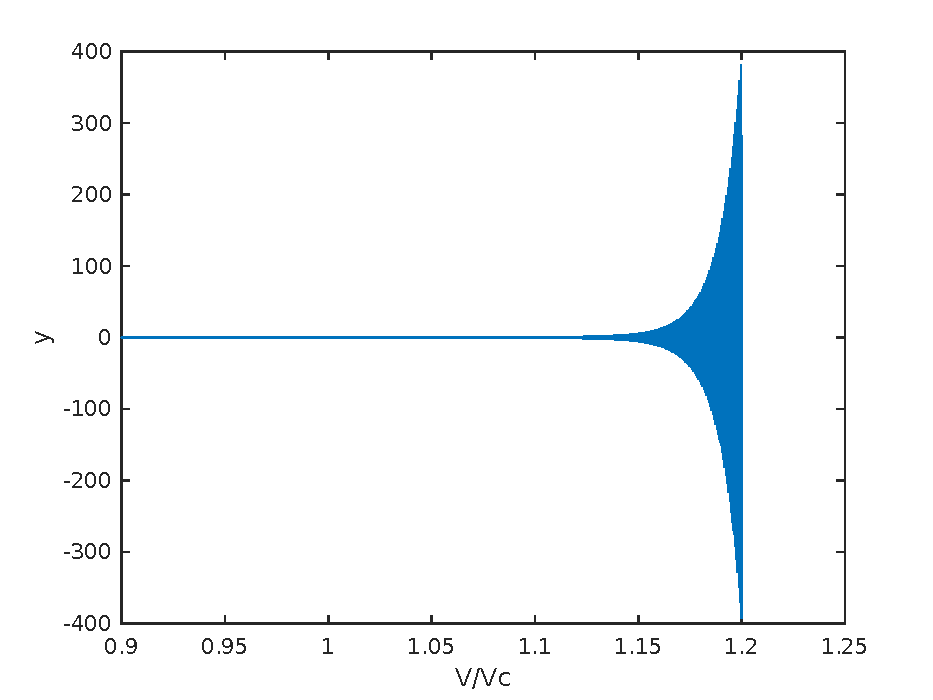
\includegraphics[width=0.4\linewidth]{./plots/linearVcSim.pdf}
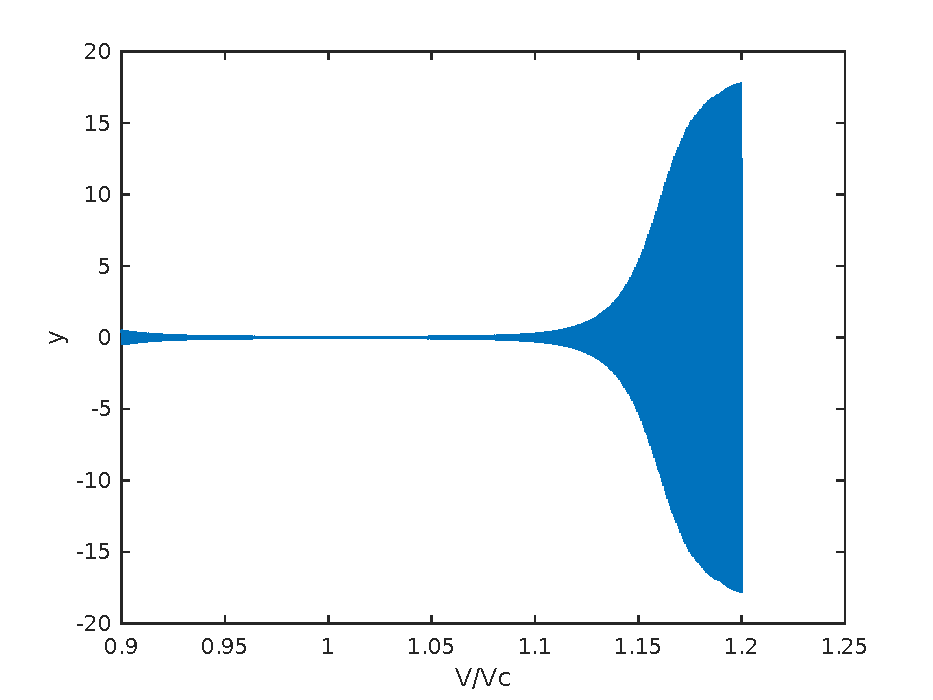
\includegraphics[width=0.4\linewidth]{./plots/nonLinearVcSim.pdf}
\caption{Linear(left) and nonlinear(right) model simulation results for wind speed values close to $V_c$}
\label{fig:linNonLinVcSim}
\end{figure}

\section{Limit cycle and bifurcation analysis}
So far only a bifurcation with respect to the stability of the fixed point at the origin has been discovered. However a closer look at the system's eigenvalues will reveal another interesting property. Considering the expression derived in \ref{eq:linSys} the eigenvalues are:
\begin{equation}
\lambda_{1,2} = -\frac{1}{2} + \frac{1}{4}VA_1 \pm \sqrt{(\frac{1}{2}-\frac{1}{4}VA_1)^2 - 1}
\end{equation}
The interesting part is the one underneath the square root. If this part turns negative the eigenvalues of the Jacobian become complex, which would lead to a Hopf-bifurcation \footnote{book page 251}. Thus the following condition is derived:
\begin{align}
(\frac{1}{2} - \frac{1}{4}VA_1)^2 - 1 &< 0 \\
(\frac{1}{2} - \frac{1}{4}VA_1)^2  &< 1 \\
(\frac{1}{2} - \frac{1}{4}VA_1) &< 1 \\
\frac{1}{2}  &< \frac{1}{4}VA_1  \\
\frac{2}{A_1} &< V \\
\end{align}
This new inequality is true when $V$ surpasses $V_c$. Using equation~\ref{eq:devVc}:
\begin{equation}
V_c < V.
\end{equation}
Thus the first bifurcation is a Hopf-bifurcation. Figures and explore what happens after this first Hopf bifurcation.

\begin{figure}
% This file was created by matlab2tikz.
% Minimal pgfplots version: 1.3
%
%The latest updates can be retrieved from
%  http://www.mathworks.com/matlabcentral/fileexchange/22022-matlab2tikz
%where you can also make suggestions and rate matlab2tikz.
%
\documentclass[tikz]{standalone}
\usepackage{pgfplots}
\usepackage{grffile}
\pgfplotsset{compat=newest}
\usetikzlibrary{plotmarks}
\usepackage{amsmath}

\begin{document}
\definecolor{mycolor1}{rgb}{0.00000,0.44700,0.74100}%
\definecolor{mycolor2}{rgb}{0.85000,0.32500,0.09800}%
%
\begin{tikzpicture}

\begin{axis}[%
width=2in,
height=2in,
at={(0.758333in,0.48125in)},
scale only axis,
xmin=-60,
xmax=80,
ymin=-1000,
ymax=1500
]
\addplot [color=mycolor1,forget plot]
  table[row sep=crcr]{%
0.5	1500\\
0.52480402245014	1463.30911016591\\
0.549044111507226	1432.5173739081\\
0.572805002431848	1406.10570159752\\
0.59615291015834	1382.95609627063\\
0.644530021762237	1341.66335470736\\
0.691587006889327	1308.42798382633\\
0.737561597011134	1280.8995290029\\
0.782632732043894	1257.22450611239\\
0.857248418428842	1223.29533284667\\
0.930011561559565	1195.51358037354\\
1.00123339986603	1172.16245453812\\
1.07115183946002	1151.94084453277\\
1.19805227723914	1120.32092088757\\
1.32175966372946	1094.64072029112\\
1.44282896357761	1073.20701720091\\
1.56168160363433	1054.7138119066\\
1.76713459270651	1027.13766962651\\
1.96765674310104	1004.64382558863\\
2.1640899484904	985.801125875674\\
2.35707624910727	969.515295075605\\
2.69253590986117	945.101758934535\\
3.02024032389568	925.159420825876\\
3.34150556922121	908.433253194335\\
3.6573363270086	893.965364770941\\
4.20675667323737	872.25844922815\\
4.74392584655937	854.498381054072\\
5.27090630212307	839.574779124777\\
5.78927025276827	826.641474228941\\
6.69417861100843	807.129742190889\\
7.57943952141084	791.093756937278\\
8.44828219020413	777.540374813693\\
9.30314827874749	765.71711740031\\
10.8064210273439	747.577427619177\\
12.2766945453241	732.428196758454\\
13.718925144324	719.364908106331\\
15.1367435348573	707.718202929385\\
17.6777603564727	688.888583439459\\
20.1545581590246	672.350761048048\\
22.5738705896211	657.227669858929\\
24.939880344631	642.910085174754\\
29.4374999776955	615.869405636391\\
33.7427751869379	588.970150999917\\
37.8529063538739	561.070401642163\\
41.7581256855934	531.411078126322\\
48.9847865332436	464.042194526752\\
55.1590442953071	386.676230576527\\
60.1460454335476	300.660474977198\\
63.841639553417	208.613850801703\\
66.6952384932747	77.593163025519\\
66.9196205243713	-55.2991842798252\\
64.5194074924169	-185.092971089963\\
59.6193075457865	-306.312359487563\\
52.9001364353044	-408.486743987133\\
44.3800272335023	-497.427837675561\\
34.3702601283164	-568.986618000152\\
23.2611632428061	-614.733626619998\\
18.5607669705415	-623.997893182914\\
13.8075892466945	-628.723307053122\\
9.03375412257598	-629.465902170289\\
4.26781226350721	-626.727606560095\\
-0.46549070141274	-620.985051073144\\
-5.14536039291897	-612.643879121024\\
-9.75281757097141	-601.936708548335\\
-14.270169010247	-588.933157750252\\
-21.9827183083339	-560.295154742648\\
-29.2585002497968	-523.785949892778\\
-35.9866548108699	-478.724734354064\\
-42.0526527671029	-424.889746827419\\
-49.3331122227744	-334.035922364041\\
-54.7574107109369	-231.341920861821\\
-58.13562672424	-121.785767233984\\
-59.379302577608	-9.01523215053896\\
-58.3651594379664	109.999903878908\\
-55.0092733112124	223.233850036915\\
-49.4642176501175	325.443862533021\\
-41.9873219539144	414.033762334461\\
-34.329180648579	477.70557217933\\
-25.6973259724682	527.584809131306\\
-16.3544786650313	560.978449820698\\
-6.5923913526664	576.134700125424\\
4.55371629900579	571.780651628268\\
15.4244253180796	547.821072671741\\
25.6379942006045	505.866863058881\\
34.8583996447195	445.768766603855\\
42.393913399868	371.744238514225\\
48.4467271434712	285.005491502624\\
52.8139833505007	189.650745271126\\
55.3749306101103	89.1714579936999\\
56.0015951873183	-32.0521917608985\\
54.0290295761308	-150.736419569398\\
49.5633120517862	-260.538822029191\\
42.8563540032142	-356.983488314862\\
35.7245276375742	-425.739358924096\\
27.4603990397888	-481.273924850063\\
18.3267712564023	-521.440767471771\\
8.62105450211227	-543.943900519921\\
-4.16808477126713	-545.524853831221\\
-16.6481311043234	-518.049973642735\\
-28.1415895984265	-463.058205111725\\
-38.0463448495382	-382.441386979434\\
-44.6446811168551	-299.065103151712\\
-49.5291352460592	-205.377138670979\\
-52.5308167255992	-105.550402825837\\
-53.5703804184449	-2.82259885543289\\
-52.574041986088	103.118890900015\\
-49.5179982286436	203.89603728593\\
-44.5387705953077	294.884710488784\\
-37.8645281928973	373.404636533128\\
-30.7861110680615	431.191216508488\\
-22.8019593452173	476.418075741584\\
-14.1479427004464	507.425612268383\\
-5.08477861172617	522.77937244543\\
6.83585157708428	518.592181825474\\
18.3490192502919	487.663963969422\\
28.8478292765435	431.121102764268\\
37.792077408546	351.446036855545\\
43.8593061175224	268.343888351735\\
48.2108256562555	176.132547931162\\
50.6961562565664	78.5919050765824\\
51.2502451072825	-21.1198659315494\\
49.8472312786754	-121.048262336598\\
46.5268854810428	-215.161133361807\\
41.4341707262412	-299.291095894512\\
34.7955568217954	-371.050008126662\\
27.7700268463868	-423.669918355215\\
19.9254798734462	-463.770194857268\\
11.4952003215426	-489.944778139943\\
2.73383816207706	-501.077239587263\\
-8.71451345287096	-492.427718909403\\
-19.6549561604065	-457.602518214586\\
-29.4936353614217	-397.834804402003\\
-37.712624075874	-316.538046700185\\
-43.1126588045676	-234.555402738107\\
-46.8307850965826	-144.861225765031\\
-48.7404270671682	-50.7529807237889\\
-48.7930936154455	44.6926071018115\\
-46.972597958041	139.328421032271\\
-43.3441817394687	227.380976506281\\
-38.0654275700744	305.049962718276\\
-31.368291544331	370.180208339103\\
-24.3478407980536	417.098276782788\\
-16.604002409856	451.389278084016\\
-8.37180555471655	471.848693185425\\
0.0956196055641527	477.62049706881\\
10.5430677943646	463.910485378738\\
20.4231638157687	427.051548316974\\
29.2349899158166	368.446696222476\\
36.5487381311224	291.61701879834\\
41.4789610717934	212.922753330013\\
44.8042768148033	127.359903056048\\
46.4126896777107	37.8845194099408\\
46.2637851284356	-52.5526280772634\\
44.3200442613645	-142.587556861667\\
40.6496693070664	-225.876852227268\\
35.4135724038988	-298.799717050247\\
28.8440860461029	-359.235292856698\\
21.9615765482522	-402.209596644184\\
14.4172330530095	-432.557533933595\\
6.44780605417145	-449.229114501517\\
-1.69433833266989	-451.526404507228\\
-11.3895452848494	-434.792796318802\\
-20.4816986094886	-396.919364504176\\
-28.5242153377122	-339.566489990145\\
-35.1413864636637	-266.271482341225\\
-39.6178511488364	-191.008298268691\\
-42.5606534299872	-109.598596477568\\
-43.8701893347286	-24.7518504365688\\
-43.5139697139607	60.662337007523\\
-41.4414528426061	145.700496366895\\
-37.7304688407382	223.822551076545\\
-32.5455862912947	291.601226632381\\
-26.1195512285485	346.963020045639\\
-19.3936056583751	385.636758212258\\
-12.0746284204905	411.676599026715\\
-4.40202663483495	424.177059633552\\
3.37218490507152	422.610483584251\\
12.3351288319434	402.487224520907\\
20.6475167542317	363.186641414825\\
27.9113818799661	306.671320167143\\
33.8006162845552	236.390118057048\\
37.7487516720434	164.258824785363\\
40.2224754585656	86.7697260097155\\
41.1362244556349	6.46921719609921\\
40.468970866946	-73.7912168468836\\
38.1756994182991	-152.918017026825\\
34.3556245099221	-224.793227538105\\
29.1794349267243	-286.270313706252\\
22.8806673421748	-335.402086470777\\
16.3015711578328	-368.775637931607\\
9.2184517936446	-389.494710618784\\
1.87406432016792	-396.819408821303\\
-5.48036927612998	-390.440123026499\\
-13.3526059966253	-367.432721051625\\
-20.5793297303124	-328.632412892678\\
-26.8495376425646	-275.979311058011\\
-31.9127885227114	-212.302139160982\\
-35.4471671403598	-144.242000854843\\
-37.5846188918215	-71.3803146757639\\
-38.2493726041058	3.85718113244212\\
-37.4276496453767	78.7029067047366\\
-35.090082794096	151.776916241463\\
-31.3435307471704	217.706008022891\\
-26.355544428337	273.596037918257\\
-20.35139010632	317.586094325533\\
-14.0270009089037	347.002248774076\\
-7.26321843347759	363.931803698171\\
-0.302949904620679	367.785023607726\\
6.60627784142878	358.446946126971\\
13.5687830271816	334.657354426118\\
19.9180090894438	297.64502082819\\
25.4029696200208	249.181348936798\\
29.8231789262263	191.576800409382\\
33.0100941313311	127.865666620607\\
34.8823307486103	59.7925540916382\\
35.3716867132781	-10.3193032264591\\
34.4695142865982	-79.8153123914676\\
32.1704973791574	-146.911909985966\\
28.5808734301846	-207.175559790161\\
23.8604020651089	-257.958214078005\\
18.2214368129043	-297.489464225741\\
12.2050720985067	-323.705366851505\\
5.80062440215238	-337.75405720978\\
-0.751944152837066	-339.178100312918\\
-7.21138801940504	-328.027020289127\\
-13.4114003399399	-304.454172183922\\
-19.0368971710549	-269.608430782604\\
-23.8792791516165	-225.059423116793\\
-27.7723960394871	-172.724763215909\\
-30.6430641027716	-113.281677769858\\
-32.2808469741234	-49.8779288364853\\
-32.6244532058828	15.260186339708\\
-31.6696564595674	79.6049996162073\\
-29.4395328285755	140.937800689688\\
-26.0350049342753	195.823935285452\\
-21.6059908795196	241.863888659233\\
-16.3497762223344	277.399404332851\\
-10.6614419085496	300.870543560136\\
-4.62877275597709	312.612008290921\\
1.51406150614909	312.276785489931\\
7.53424692315826	300.040387264322\\
13.0920625198349	277.131190117484\\
18.1130588258328	244.441488872398\\
22.4194539156346	203.354555913022\\
25.8697260709275	155.499598822077\\
28.4484313836757	100.052656350456\\
29.872255139139	41.0278846820163\\
30.0865602944847	-19.4428557455061\\
29.0912353044377	-78.9639468741424\\
26.939769960386	-134.893801893415\\
23.7245234153623	-184.779877602323\\
19.584854396617	-226.466597895465\\
14.7023236716962	-258.425624559812\\
9.34268258915744	-279.508905998336\\
3.67673350679208	-289.381227652434\\
-2.06945131181141	-287.781865640597\\
-7.67303349036011	-274.972325957833\\
-12.6905836077239	-252.933235223348\\
-17.2060312046414	-222.266664400199\\
-21.0645443904496	-184.199086826539\\
-24.1428467733767	-140.148881320778\\
-26.4588587142006	-88.3647416139063\\
-27.6928504547445	-33.3594216195238\\
-27.7964110061958	22.8290805683562\\
-26.7730746182784	77.9380803637467\\
-24.705729443744	128.962294024659\\
-21.6758354010413	174.340537629071\\
-17.8122072453558	212.143754686569\\
-13.2810645035649	240.977656207909\\
-8.23953808213457	260.020401596946\\
-2.92403495294228	268.413419858596\\
2.44899719897873	265.958595752128\\
7.66751447453351	252.968041290117\\
12.2329085639149	231.901521155273\\
16.3278388215949	203.104666237829\\
19.8148361151819	167.676963526016\\
22.5844084502762	126.881095804006\\
24.6722890981405	78.4284728618463\\
25.7455495730641	27.0723379928315\\
25.76129399731	-25.2434263609718\\
24.7259758801934	-76.3869101733864\\
22.7477023214189	-123.084518392359\\
19.8960262346406	-164.518076950379\\
16.2897286212929	-198.9579343102\\
12.0808073307266	-225.135461738018\\
7.34024059091568	-242.476813403967\\
2.35229849209659	-249.739092095499\\
-2.67694791075749	-246.766127138617\\
-7.54642273695084	-233.89306582858\\
-11.7348321903842	-213.844283400426\\
-15.4815779304693	-186.768755744888\\
-18.6624894870723	-153.664295129742\\
-21.1786298268017	-115.676271533591\\
-23.0739520881307	-70.2449109543977\\
-24.016607236466	-22.1817985945254\\
-23.9683469799207	26.6628052770911\\
-22.9377087615782	74.2827044635172\\
-21.0518790191138	117.242176648514\\
-18.3689488676964	155.295695082459\\
-14.9984960082748	186.882590101772\\
-11.0798198417889	210.844773012752\\
-6.61948292606955	226.789938587387\\
-1.93314069308153	233.212574177948\\
2.78365494721878	229.982285287051\\
7.34051638138499	217.437947520644\\
11.2142793034373	198.410959528274\\
14.6725589401861	172.915496697399\\
17.6015131711688	141.867592809392\\
19.9103983538857	106.321863859994\\
21.6457269129943	63.6249418611898\\
22.4850154872218	18.5227541828833\\
22.3938023814676	-27.2258914242367\\
21.3819350852053	-71.7330793138985\\
19.5892050034199	-111.495767395368\\
17.0636988835436	-146.681549169713\\
13.9067655427207	-175.870115055372\\
10.2466279916374	-197.997331466336\\
6.04432398603636	-212.800065959838\\
1.63304169997524	-218.608423518291\\
-2.80191865451106	-215.306287726813\\
-7.08031264150182	-203.224008674546\\
-10.6897514309745	-185.192039690193\\
-13.9074552754032	-161.141793260545\\
-16.627747921966	-131.922611152389\\
-18.7663567146217	-98.516834886056\\
-20.3691822185868	-58.29070670118\\
-21.1274817270636	-15.8460647180049\\
-21.0098306966358	27.1458679712436\\
-20.0267688530772	68.9065874119301\\
-18.3250515604113	105.938572747791\\
-15.9446108638871	138.691602914251\\
-12.9795448652716	165.86139503631\\
-9.5485199881358	186.462696858268\\
-5.58206315889437	200.322610254095\\
-1.42028905295955	205.680682391209\\
2.76124388382146	202.427560533788\\
6.79176136927621	190.878098978274\\
10.1767853491389	173.793390406152\\
13.1915799613341	151.060655085451\\
15.7370665247278	123.473848981616\\
17.7341929517679	91.9560833932137\\
19.2265908999634	53.9605218669675\\
19.9211729313683	13.9007722597619\\
19.7889506574463	-26.6344536987729\\
18.8407134635304	-65.9666964909676\\
17.2258588079412	-100.653862680771\\
14.9779462538073	-131.329490999778\\
12.1847229996287	-156.785762161028\\
8.95662465131244	-176.103796831499\\
5.20480670770527	-189.173086740902\\
1.26883199935861	-194.194950270791\\
-2.68485098849511	-191.06227524952\\
-6.49422459956455	-180.071062073756\\
-9.68626720987557	-163.87377574792\\
-12.5275443074271	-142.339475469535\\
-14.9244363264941	-116.21523750414\\
-16.8022045166855	-86.3743409416135\\
-18.2014464792986	-50.3927840137484\\
-18.8451623610071	-12.4759719113264\\
-18.7063406107457	25.8642098075321\\
-17.7957295208868	63.0401726953972\\
-16.2623597239789	95.6960600825412\\
-14.1349125573373	124.579457306198\\
-11.4955725896097	148.563690533702\\
-8.44765812348544	166.786309850325\\
-4.89080580305803	179.179761515774\\
-1.15913646719644	183.94247119754\\
2.58933719839674	180.967095710014\\
6.2006512894008	170.529717542693\\
9.22453395954513	155.154935303929\\
11.9152794737534	134.709854981065\\
14.1838945410171	109.901159837947\\
15.9592914611176	81.5592350171037\\
17.2787791313726	47.3983929353937\\
17.8810324554076	11.4117047755972\\
17.7406738565144	-24.9599552806772\\
16.8682343282381	-60.2113013456609\\
15.4104452110874	-91.0894972535692\\
13.3922678450316	-118.408773072468\\
10.8909973602323	-141.11169033513\\
8.00375421825862	-158.384440278358\\
4.62398527638993	-170.189044309606\\
1.07741495575953	-174.743868842377\\
-2.48571208563186	-171.940178155593\\
-5.91882106978851	-162.034429347271\\
-8.79433174524675	-147.41701571138\\
-11.3526993564892	-127.962369232644\\
-13.5089385970592	-104.34182072039\\
-15.1951227932541	-77.348121640944\\
-16.4452992614555	-44.836809810411\\
-17.0129620124054	-10.5940756817533\\
-16.874112860144	24.0045927939239\\
-16.038968374799	57.5284394594134\\
-14.6508174695465	86.8349603480078\\
-12.7317610629332	112.773703291205\\
-10.3547733373796	134.347155601472\\
-7.61153292444814	150.784035117842\\
-4.39280893466105	162.066788797257\\
-1.01432283295966	166.447800362171\\
2.380814828763	163.816564057999\\
5.65280505999578	154.41093883085\\
8.39593756275955	140.488552569706\\
10.8364752190991	121.935904644511\\
12.892972138699	99.3929724514666\\
14.5002928120529	73.6189714441913\\
15.6893964237595	42.6063582353188\\
16.2275435961417	9.9451320576657\\
16.0919249473637	-23.0493483033057\\
15.2923966725715	-55.0139276240624\\
13.968199485749	-82.9177590462826\\
12.1391988653419	-107.625424982189\\
9.87452680524778	-128.191969724409\\
7.26104370900451	-143.88377750947\\
4.18909893567864	-154.697472073829\\
0.963693179573314	-158.927610462759\\
-2.27861060099315	-156.461976223682\\
-5.40423152211754	-147.521201935109\\
-8.02811627031255	-134.235921698474\\
-10.3626796737812	-116.506643935485\\
-12.3296513236397	-94.9452311335972\\
-13.8664007800588	-70.2806391699498\\
-15.0010397250251	-40.6341817152645\\
-15.5134906383893	-9.41276605370624\\
-15.381987752783	22.1235682599613\\
-14.6160122987172	52.6731503193314\\
-13.3504971034086	79.3145655192761\\
-11.6035245665727	102.914506488971\\
-9.44078854062878	122.574647537932\\
-6.94484927006935	137.595108908948\\
-4.00705306439563	147.982411396399\\
-0.921521211730196	152.077545751829\\
2.18119676414924	149.76686428611\\
5.17323549767119	141.255257015251\\
7.68882210204968	128.554268052507\\
9.92723847338663	111.578724484757\\
11.8130995244055	90.9150465632461\\
13.2860526054481	67.2646137845439\\
14.3716244700305	38.8679155649073\\
14.8613228867455	8.96255098630886\\
14.7343125394869	-21.2424138971317\\
13.9997033023035	-50.501417584574\\
12.7880729413028	-75.9983072847589\\
11.1160504146559	-98.593770439783\\
9.04623405011924	-117.431262707719\\
6.65731817568607	-131.841402295377\\
3.84250907527683	-141.837657857421\\
0.885225465482799	-145.809209948343\\
-2.08951466816682	-143.641350558778\\
-4.95911079582118	-135.524692251697\\
-7.37566426628377	-123.360388567749\\
-9.52620994522981	-107.077005122345\\
-11.3380107433766	-87.2377627528042\\
-12.7528064147392	-64.5187086015213\\
-13.7937984445219	-37.2694579960476\\
-14.26307246715	-8.57178694746302\\
-14.1406331982292	20.412312787564\\
-13.4352326212685	48.4886716453178\\
-12.2731704608561	72.9412907215274\\
-10.6698659276479	94.6198426591997\\
-8.68511410806359	112.705533153813\\
-6.39411081525751	126.556763189722\\
-3.69242574739113	136.191899191177\\
-0.853141409850595	140.048494796203\\
2.00382330364612	138.011171623622\\
4.7607295164181	130.257643502462\\
7.08619166501784	118.587397471514\\
9.15593616336007	102.941719610831\\
10.8996752438241	83.8625406633629\\
12.2610861341424	62.0024860290905\\
13.2612890700766	35.8105659550719\\
13.7120267219325	8.22540971414474\\
13.594069822125	-19.6345778032367\\
12.9158307047479	-46.6224744011801\\
11.7994761159131	-70.116997350084\\
10.2593991473269	-90.9537878272975\\
8.35284262097437	-108.348400484963\\
6.15181752901547	-121.684706480533\\
3.55452920055303	-130.984529845713\\
0.824187532788463	-134.733020015601\\
-1.92400057322033	-132.814499224707\\
-4.57679741060416	-125.395044718853\\
-6.81805260455923	-114.180810217553\\
-8.81310875130514	-99.1246105773317\\
-10.4939577056668	-80.7487318051497\\
-11.8060819366927	-59.6840287433282\\
-12.7687431687747	-34.4698367269732\\
-13.2025109018811	-7.91328235433899\\
-13.0888599613752	18.9076994563546\\
-12.4358830627676	44.8897839337018\\
-11.3617924876578	67.5009872888689\\
-9.88009655309693	87.5611777770526\\
-8.04570274773158	104.317352824173\\
-5.9277073733373	117.17685779874\\
-3.42707623469574	126.16395084948\\
-0.797650731032653	129.810036308321\\
1.84972793354207	127.999471334882\\
4.40600070275865	120.887833401438\\
6.56907415418849	110.095684967068\\
8.49478266512414	95.5861523138211\\
10.1172503192179	77.8633093452495\\
11.3836499713045	57.5376850060437\\
12.3115846649729	33.2306705035022\\
12.7297079785319	7.62844327616415\\
12.6201460429971	-18.2287435625016\\
11.9906920939979	-43.2779379325185\\
10.9557952163426	-65.0712484362775\\
9.52819012087636	-84.4118442601797\\
7.76063767069194	-100.575655024412\\
5.71955392179977	-112.991758624376\\
3.30869702373294	-121.686111199678\\
0.773050648910376	-125.234721941695\\
-1.78059969394182	-123.522274311475\\
-4.24708461396626	-116.694860260587\\
-6.33729291748183	-106.294527413016\\
-8.19836105023614	-92.2935484559253\\
-9.7664155512094	-75.1790436410806\\
-10.990218471954	-55.5424928713257\\
-11.8858916317958	-32.0799002466702\\
-12.2895107362072	-7.36598809891587\\
-12.1838075184704	17.5941734408976\\
-11.5762950869369	41.7751453801789\\
-10.5778513665661	62.808226392441\\
-9.20052670912654	81.4794815689237\\
-7.49510051376317	97.0915835916944\\
-5.52551351828323	109.093809277284\\
-3.19829027847651	117.513277063621\\
-0.750054755725839	120.968803180739\\
1.71618530079368	119.345645731168\\
4.0988906959856	112.781311342992\\
6.12095821164462	102.745739348801\\
7.9215659532228	89.2192732281922\\
9.43872739742489	72.6731934361694\\
10.6227036257634	53.6810689056123\\
11.4882919149791	31.0068656054974\\
11.8784009458682	7.1223603132159\\
11.7763279796259	-17.000314706013\\
11.1893241337882	-40.3706877774554\\
10.2248823433506	-60.6946864096422\\
8.89444160108821	-78.7411991514034\\
7.24694523074794	-93.8377176190962\\
5.34403894192775	-105.452357007755\\
3.09495265638307	-113.613003903493\\
0.728425407330094	-116.979436944397\\
-1.65606310780226	-115.437697122135\\
-3.96037035914488	-109.117502747961\\
-5.91852079578385	-99.4224541250476\\
-7.66240374535016	-86.3399931799382\\
-9.13181588449701	-70.3265529584958\\
-10.2784362483564	-51.9388129657677\\
-11.115875513966	-30.0027794313256\\
-11.4933508140367	-6.89490121902617\\
-11.3946894365095	16.4436043385298\\
-10.8268972640183	39.0549574721605\\
-9.8942591314126	58.715499124801\\
-8.60766337882616	76.1770800702432\\
-7.01434593107189	90.7903079673346\\
-5.17381702155752	102.040921761231\\
-2.99793044575411	109.957283285349\\
-0.707986825727945	113.238304170508\\
1.59983729802221	111.770980685329\\
3.83058532391506	105.677948019393\\
5.72861499424226	96.3016492737598\\
7.41913021284965	83.6357569324543\\
8.84361702868618	68.122745935732\\
9.95509899534579	50.3033288046269\\
10.7661215200645	29.060286951347\\
11.1317425532708	6.68156281335708\\
11.0362876958372	-15.9207129452571\\
10.4865329531656	-37.8194106690759\\
9.58372116318076	-56.8574026327322\\
8.33824122706198	-73.7697732296665\\
6.79573613382185	-87.9287299691544\\
5.01372260264319	-98.8365453349167\\
2.90658579801797	-106.521836868851\\
0.688604400918837	-109.720871988111\\
-1.54714512075785	-108.32174333025\\
-3.70870140373362	-102.440627277664\\
-5.55003867921718	-93.3634600611042\\
-7.19021784567352	-81.0893759699382\\
-8.57232895933969	-66.0476928830586\\
-9.65067318240629	-48.763993599287\\
-10.4368374045496	-28.1731526218787\\
-10.7913026116609	-6.48072276091929\\
-10.698864191373	15.4285945523281\\
-10.166082290306	36.6564805780703\\
-9.29131266146852	55.1087690406285\\
-8.08448851037553	71.5041307542789\\
-6.58976219302461	85.2350159076115\\
-4.86278385153501	95.8192473877733\\
-2.82037256317904	103.285532725832\\
-0.670171600359722	106.405791091244\\
1.49765874698542	105.069325690552\\
3.59397932240004	99.3864075641439\\
5.38173350570785	90.5906408459931\\
6.97432642680024	78.6859437166797\\
8.3163741000979	64.0892018861614\\
9.36339403136983	47.3116318077528\\
10.1261086283745	27.3360326434239\\
10.4700477328302	6.29106343038525\\
10.3804507120552	-14.9644964419498\\
9.86367462845372	-35.5594763074703\\
9.01533208215766	-53.4593891150821\\
7.84493834469664	-69.3668927167019\\
6.39524697904558	-82.6934593420185\\
4.72015557136298	-92.9715720138239\\
2.73881856590961	-100.229902480659\\
0.652601584144388	-103.274401550562\\
-1.45108427854553	-101.995674323481\\
-3.48576462679994	-96.4985780798528\\
-5.22276656965913	-87.968136887694\\
-6.77027722510795	-76.4124564286222\\
-8.07436690525121	-62.2366489821659\\
-9.09171312925813	-45.9382634512865\\
-9.832256798983	-26.5443059157456\\
-10.1662405625653	-6.11149138247278\\
-10.0793243051492	14.5259481038182\\
-9.57767364446809	34.5224812248915\\
-8.75429151647315	51.9002803690087\\
-7.61830815617683	67.346416722058\\
-6.21116112315987	80.2902819614324\\
-4.58509830007204	90.2782100480894\\
-2.66151228814105	97.3387411506756\\
-0.635821746517633	100.310325812584\\
1.40715937471124	99.0849430222371\\
3.38347778352749	93.7624738873304\\
5.07231396595622	85.4827399833079\\
6.57703067823552	74.257510351615\\
7.84508649502424	60.4807247617499\\
8.83426697006136	44.6369065370004\\
9.55380486755732	25.7939456581504\\
9.87835296968027	5.94108265263868\\
9.79397025888533	-14.1107402617575\\
9.30664152273961	-33.5402575956096\\
8.50688376889643	-50.4235194789027\\
7.40347108336524	-65.4324477840258\\
6.0365999438499	-78.0133537320294\\
4.45696167190984	-87.7256841933779\\
2.58809263513899	-94.5977746739912\\
0.61977009260405	-97.4991320238539\\
-1.36565032093786	-96.3231648558297\\
-3.28660498702065	-91.16516857135\\
-4.92964634639167	-83.1228086728931\\
-6.39366725785562	-72.2110569621312\\
-7.62745351117224	-58.8132308100356\\
-8.58985057991525	-43.4014196427445\\
-9.2894481111795	-25.081419940813\\
-9.605035615334	-5.77904469999829\\
-9.52305154210012	13.7169001189242\\
-9.04930954304528	32.6081604094813\\
-8.27195542552265	49.0220976957997\\
-7.19943266846205	63.6159232969328\\
-5.87076471635771	75.8519578960992\\
-4.33517098781201	85.3020860275954\\
-2.5182409109948	91.9943828191102\\
-0.604392779114866	94.8280542855742\\
1.32634898936745	93.6979807666475\\
3.19468989242509	88.6952212603762\\
4.79411638675328	80.8780388467505\\
6.21937113978313	70.2642031213819\\
7.4205105570528	57.2269142974959\\
8.35739536897254	42.2263748563211\\
9.03802986578909	24.4036132258293\\
9.34509259911067	5.62468929819964\\
9.26538343647801	-13.3426661445924\\
8.80455376375041	-31.7220611901985\\
8.04848465118068	-47.68979694605\\
7.0053116917699	-61.8888080216828\\
5.71294731503905	-73.7965934386722\\
4.21921624691424	-82.9968557762995\\
2.45167441495456	-89.517367453645\\
0.589642403604157	-92.2857591773264\\
-1.28906992346717	-91.1984137102295\\
-3.10732631681488	-86.3424669335037\\
-4.66514798632579	-78.7392741711444\\
-6.05341629667492	-68.4090464382289\\
-7.22340565665432	-55.7153322249716\\
-8.13595048937596	-41.106954052772\\
-8.79852116407873	-23.7577635043589\\
-9.09746024447885	-5.47741274248104\\
-9.01991236955594	12.986464099184\\
-8.57137479305932	30.8782814938863\\
-7.83556275742292	46.4210840328748\\
-6.8203242905609	60.2439544597604\\
-5.56251751156884	71.8388087314413\\
-4.10864309749391	80.8005973338534\\
-2.38814125361551	87.1567580360455\\
-0.575476782939078	89.8621500402877\\
1.25364765565341	88.8146797041359\\
3.02415186625367	84.0978415039371\\
4.54222699464989	76.6983483061872\\
5.89515465796921	66.63853856925\\
7.03537824456832	54.272739034954\\
7.92466710021817	40.0388633928709\\
8.57000358899996	23.1414112440846\\
8.86118927223851	5.33668104785217\\
8.78569816545469	-12.6468850720884\\
8.34888086508588	-30.073535297912\\
7.6323788047454	-45.2110204111923\\
6.64377070892199	-58.6749845687816\\
5.41891238996242	-69.9710610801004\\
4.00304530682769	-78.7049223714661\\
2.32741608402042	-84.9036477337103\\
0.561858057401672	-87.5482022055414\\
-1.21993429808297	-86.5380289691285\\
-2.94484240698659	-81.9532350670103\\
-4.4248932616986	-74.7479527458698\\
-5.7440060214323	-64.9463709229023\\
-6.85574727339108	-52.8939928558028\\
-7.72278504478385	-39.0182622412641\\
-8.35165478193167	-22.5523574431889\\
-8.63542975804888	-5.20201862494133\\
-8.56189909132438	12.3226657974492\\
-8.13627360600564	29.3048792934182\\
-7.43820666592623	44.0551852293917\\
-6.47502417452093	57.1761893618714\\
-5.28162746659964	68.18659779581\\
-3.90205844815717	76.702318496274\\
-2.26929658252553	82.7500548173726\\
-0.548752015917789	85.3358236908017\\
1.18779740995262	84.3606117426692\\
2.86910728555244	79.9013681222081\\
4.31273382306154	72.8815254792898\\
5.59944944327831	63.3268784989929\\
6.68390109198842	51.5744767604758\\
7.52962153303685	38.0417036315925\\
8.14273614894782	21.9886288201698\\
8.41941838711157	5.07299943240786\\
8.34775920249545	-12.0126712415045\\
7.93283600371243	-28.5696700744164\\
7.25239409998527	-42.949609609997\\
6.31352150873238	-55.742443477462\\
5.15020919615488	-66.4793551739305\\
3.80535457344732	-74.786037349588\\
2.21360048856303	-80.6888049865245\\
0.536127574713729	-83.2177369470643\\
-1.1571181260739	-82.275364427651\\
-2.7966852025768	-77.9356866573108\\
-4.2053770527799	-71.0931566966957\\
-5.46101587443442	-61.7749585290915\\
-6.51928880604039	-50.3100322349686\\
-7.34456149494637	-37.1060840735966\\
-7.94258239311768	-21.4484486745591\\
-8.212467612023	-4.949239931289\\
-8.1425975869758	11.7158793205455\\
-7.73792219286953	27.8655272780381\\
-7.07435347935832	41.890720424964\\
-6.15875515950363	54.3691322855135\\
-5.02424861306253	64.8438724009077\\
-3.71263769196406	72.9499992852909\\
-2.16016311003538	78.7134310891925\\
-0.523956364843837	81.1873780762286\\
1.12778952316761	80.2759125851427\\
2.72734065149281	76.0502728108063\\
4.10248763854245	69.3775085416252\\
5.32828184695668	60.2860012851374\\
6.36141288135392	49.0969026559084\\
7.1670493298579	36.2086009868286\\
7.75059256898595	20.9302123104935\\
8.01395639381106	4.8303933786908\\
7.94579918669793	-11.431367549559\\
7.5509487436595	-27.1903018260913\\
6.90355388445029	-40.875292084321\\
6.01026640954272	-53.0520895054583\\
4.90337590997018	-63.2752179370198\\
3.62363991286037	-71.1887118800684\\
2.10883520380038	-76.8180873495681\\
0.51221239878666	-79.2388106090174\\
-1.09971519765707	-78.356487945157\\
-2.66086084263292	-74.2397684708284\\
-4.00376225489445	-67.7297465075717\\
-5.20086404624828	-58.8558309573645\\
-6.20982279142932	-47.9316850320502\\
-6.9965818258574	-35.3467164098515\\
-7.56622241045427	-20.4324661709381\\
-7.82332226527067	-4.71614513693153\\
-7.75680693359404	11.1583014053466\\
-7.3713872022898	26.542048524104\\
-6.73951433526019	39.9004050905995\\
-5.86763956106173	51.7875436558664\\
-4.78725579419666	61.7689263554395\\
-3.53811813873098	69.4972000220993\\
-2.0594811639994	74.9974757405652\\
-0.500871795799658	77.3666514663813\\
1.07280802907379	76.5118571359244\\
2.59705304300566	72.4993096713341\\
3.90892582892177	66.1454805413341\\
5.07841463164627	57.4806549141883\\
6.06410954471764	46.8112886125548\\
6.83270206280167	34.5181259096776\\
7.38897772775846	19.9538900180515\\
7.64005450305878	4.60620876732079\\
7.57511498681321	-10.8959241929466\\
7.19875767843834	-25.9190023762838\\
6.58179797331049	-38.9634103124791\\
5.73049693625486	-50.5720719420432\\
4.67558349386684	-60.3209439717675\\
3.45585121919175	-67.8709457255237\\
2.01197746526121	-73.2467825604951\\
0.48991255193708	-75.5660071556625\\
-1.04698910497452	-74.7372602513102\\
-2.53574227156118	-70.8244700426922\\
-3.81772830927739	-64.6207142787354\\
-4.9606171905898	-56.1570199771091\\
-5.92390095501944	-45.7328992340736\\
-6.67499414507303	-33.7207318275047\\
-7.2184087052264	-19.4932816347127\\
-7.46368823307654	-4.50032274074096\\
-7.40026289593357	10.6435482201402\\
-7.03262331222329	25.3195580684855\\
-6.43000704150279	38.0618981016541\\
-5.59849456251195	49.4025604246529\\
-4.56808130936039	58.9275818871659\\
-3.37663749068217	66.3058361429928\\
-1.96621131853614	71.5616236143044\\
-0.479314344766318	73.8324185973577\\
1.02218678567667	73.0283577115097\\
2.47676929839242	69.2112118889469\\
3.72994186346423	63.1518011258298\\
4.84718323045722	54.8817745959328\\
5.78885754150449	44.6939484893776\\
6.5230786365173	32.9526201609494\\
7.0541049606845	19.0495436278632\\
7.29379932438325	4.39824764074992\\
7.23183054597151	-10.4005471049283\\
6.87258548316122	-24.7422521538404\\
6.2837785368893	-37.1936715201387\\
5.47131843502354	-48.2761695076469\\
4.4644956246519	-57.5854753041488\\
3.30029264215608	-64.7981185125791\\
1.92207950549124	-69.9379966764632\\
0.469058365572564	-72.161813256778\\
-0.998335889689078	-71.38118414212\\
-2.41998890396135	-67.6558437160733\\
-3.64535844019035	-61.7354061276768\\
-4.73784912787065	-53.6520360095286\\
-5.65866896378612	-43.6920869664468\\
-6.37660859158902	-32.2120405116639\\
-6.89569125111043	-18.6216719953413\\
-7.12999995176656	-4.29976376548327\\
-7.06943376496075	10.1663490618892\\
-6.7182796475871	24.1857475470417\\
-6.14278043328079	36.3567230646577\\
-5.34868126833574	47.1903039444236\\
-4.36459430820578	56.2915481669736\\
-3.22664785701717	63.3443609902183\\
-1.87948736374522	68.3722401374828\\
-0.459127173752527	70.5504634807795\\
0.975376983180274	69.7921082149768\\
2.36526836104191	66.1549832384783\\
3.56378764360379	60.3684727505577\\
4.63237346827537	52.4651616373717\\
5.53305091306219	42.7251609394504\\
6.2352660943682	31.4973886292851\\
6.74282372847677	18.2087461810551\\
6.97193472731921	4.20466905668431\\
6.91272049511654	-9.94043103319705\\
6.56937171041479	-23.6488199939359\\
6.00670838830067	-35.5492143738994\\
5.23031966363089	-46.14258669324\\
4.26816444521691	-55.0429823363748\\
3.15554819022677	-61.9414184942158\\
1.83834790021398	-66.8609969194558\\
0.449504569423507	-68.9949501236769\\
-0.953255759087202	-68.2577975714743\\
-2.31248610772265	-64.7055250552765\\
-3.4850548745954	-59.0481938518084\\
-4.53053471939437	-51.318724075868\\
-5.41174239317445	-41.7911919993017\\
-6.09875923158943	-30.807191164073\\
-6.59518666556626	-17.8099203926859\\
-6.819277317882	-4.11277729987534\\
-6.76136744507681	9.72231354857197\\
-6.42555485285792	23.1303462348423\\
-5.87528286380793	34.7694584871594\\
-5.11599163080134	45.1308360620153\\
-4.17501035275481	53.8371906381274\\
-3.08685114638634	60.5864028321262\\
-1.79858101375777	65.4011828962215\\
-0.440175481186049	67.4921306968441\\
0.931922493512262	66.775188093737\\
2.26153058463776	63.3046123214296\\
3.40899970137273	57.7719862318066\\
4.43212919111516	50.2104891776965\\
5.29450333603477	40.8883591972942\\
5.96681943773066	30.140092306152\\
6.45248958452913	17.4244159955804\\
6.67172747873293	4.02391655160384\\
6.61507715418545	-9.5115562145469\\
6.28654675059083	-22.6292936231949\\
5.74824660030218	-34.0159042911302\\
5.00547441441504	-44.1530456723925\\
4.08495183734916	-52.671793231364\\
3.02042543022668	-59.2766564981658\\
1.76011281150937	-63.9899591769943\\
0.431125866666753	-66.0391113998972\\
-0.911331568801355	-65.341456907617\\
-2.2122992136345	-61.9496118482007\\
-3.33547442734238	-56.5374682610507\\
-4.33696924178311	-49.1383967775162\\
-5.1811125046264	-40.0149833451804\\
-5.83919916002776	-29.4948420424545\\
-6.31446473165395	-17.0515148279611\\
-6.52900844502112	-3.93792775843106\\
-6.47357541084289	9.30775374764658\\
-6.15208712735729	22.1447109976516\\
-5.62536239547511	33.2871228486111\\
-4.89856258085871	43.2073668473471\\
-3.99782266104965	51.5445968306119\\
-2.95614984550169	58.0097296265859\\
-1.72287500580786	62.6247077139052\\
-0.422342623957613	64.6332224929711\\
0.891441054234951	63.953998598993\\
2.16469749852774	60.6380921570648\\
3.26434282923999	55.3424401558249\\
4.24488169706689	48.1005436968845\\
5.07136564405232	39.1695131721313\\
5.71566979940776	28.8702858057811\\
6.18086485066184	16.6905533081132\\
6.39086463161708	3.85466353910252\\
6.33660897606269	-9.11053247837661\\
6.02193559770415	-21.6757206364272\\
5.50641114493857	-32.5817953501708\\
4.79506633068303	-42.292093088202\\
3.9134691873404	-50.4535763882466\\
2.89391232204794	-56.7833596667879\\
1.68680438074308	-61.3030097779204\\
0.413813512422608	-63.271996553633\\
-0.872212336580855	-62.6104042054489\\
-2.11863823147412	-59.367804085275\\
-3.19547904252995	-54.1848665424303\\
-4.15570645269638	-47.0951687186552\\
-4.9650738471439	-38.3505130859041\\
-5.59601989007812	-28.2653553259279\\
-6.05146121416418	-16.3409172248671\\
-6.25705959964907	-3.7739871064934\\
-6.20394357091523	8.91954726336514\\
-5.89586975968194	21.2215111482434\\
-5.39119010964983	31.8987024692891\\
-4.69481000573434	41.4056463581192\\
-3.83174918271129	49.3968589043861\\
-2.83360905388211	55.5954534125631\\
-1.65184231902887	60.0226269172533\\
-0.405527081633638	61.953149231635\\
0.853609793866878	61.3084426121889\\
2.07404079093238	58.1366636025968\\
3.1287665745295	53.062861004913\\
4.06929523668737	46.120639268384\\
4.86206210617594	37.556652324306\\
5.48005348612395	27.6790605221063\\
5.92604187901783	16.002037119682\\
6.12737425430729	3.69577130997183\\
6.07536209279844	-8.734478752082\\
5.77368350429418	-20.7813311759795\\
5.27951137994008	-31.2367149344323\\
4.597630765271	-40.5465649317675\\
3.75253075333541	-48.3727090815851\\
2.77514373377708	-54.4440710733311\\
1.61793438132112	-58.7814840704242\\
0.397472607396594	-60.6745621727408\\
-0.835600506701135	-60.0460440366551\\
-2.03083051922667	-56.9427365497195\\
-3.06409742857951	-51.9746723569609\\
-3.98551051025431	-45.1754395797214\\
-4.7621680264426	-36.7866953151733\\
-5.3675887281526	-27.110482300168\\
-5.80441013639634	-15.6733841826634\\
-6.00160524376207	-3.61989778212329\\
-5.95066303069489	8.55503096210033\\
-5.65518551343107	20.3544838071047\\
-5.17120051053608	30.5947851590703\\
-4.50337740909417	39.7134926065767\\
-3.67569139936025	47.3795165835703\\
-2.71842687191123	53.3274121214791\\
-1.58502993127375	57.5776545545194\\
-0.389640034007305	59.434267831281\\
0.818154002264766	58.8212853327151\\
1.98893816945779	55.7842250514104\\
3.00137132500371	50.9186724167472\\
3.90422448964129	44.2581601535085\\
4.66524068097599	36.0394930898638\\
5.25845656695209	26.5587661383228\\
5.68638313165406	15.3544665963751\\
5.87956353344647	3.54625617622144\\
5.82965905393538	-8.38092912350002\\
5.5401979221538	-19.9403216004103\\
5.06609530470762	-29.9719397938246\\
4.41190932894178	-38.9051691007131\\
3.60111717186329	-46.4157846923831\\
2.66337518797671	-52.2438026886721\\
1.55308180059346	-56.4093466897954\\
0.382019922005599	-58.2304359317043\\
-0.801242026799597	-57.6323768842043\\
-1.94829941296469	-54.6594553931427\\
-2.94049500663464	-49.893345095422\\
-3.82531827363484	-43.3674883478231\\
-4.57113958864826	-35.3139756177396\\
-5.15249962442674	-26.0231163619394\\
-5.57179063263078	-15.0448262710568\\
-5.76107313364807	-3.47474348310697\\
-5.71217575265046	8.21191775837555\\
-5.42855512467045	19.5382421512583\\
-4.96404472882045	29.3672730842946\\
-4.32309557207316	38.12042148813\\
-3.52870191965778	45.4801201878521\\
-2.6099110676431	51.1916843165268\\
-1.5220459891712	55.2748918558589\\
-0.374603400798232	57.0613613735032\\
0.784838342998442	56.4776508902802\\
1.90885439978462	53.5668671798534\\
2.88138161840478	48.8972766367788\\
3.74868106367526	42.5021999592131\\
4.47973380041281	34.6091449477389\\
5.04957117485789	25.5027910220725\\
5.46047392806019	14.7440359227558\\
5.64596996146884	3.40526341760929\\
5.59805051116935	-8.04775896639176\\
5.32010270625363	-19.1476841287237\\
4.86490794120461	-28.7799409347158\\
4.23681400323958	-37.3581565421172\\
3.45834661493375	-44.5712242981163\\
2.55796207553614	-50.1696038944842\\
1.49188139605126	-54.1727338033987\\
0.367382125613471	-55.9254534026702\\
-0.768918549206954	-55.3555508726356\\
-1.87054736559773	-52.5050036207865\\
-2.82395015195553	-47.9291468682383\\
-3.67420946529002	-41.6611516748467\\
-4.39090108053338	-33.9240690592093\\
-4.94953423188029	-24.9970973043861\\
-5.35228484028254	-14.4516964528301\\
-5.53410082083705	-3.33772586627353\\
-5.48713149822845	7.88823089103486\\
-5.2146964858217	18.7681237269837\\
-4.76855342149178	28.2091555912601\\
-4.15295055314554	36.6173538766596\\
-3.38995874823917	43.6878845909478\\
-2.50746051797411	49.1762046408303\\
-1.46254957758201	53.1014190697293\\
-0.360348238322084	54.8212258971663\\
0.753459917760981	54.2646222579421\\
1.83332627953522	51.472502805741\\
2.76812494744817	46.987721342456\\
3.60180686110832	40.8432742917824\\
4.30452717145759	33.257876337392\\
4.8522607285588	24.5053874051336\\
5.24708483861838	14.1674345929389\\
5.42532248648248	3.27204638919428\\
5.37927676005184	-7.73312634485994\\
5.11220165598572	-18.3990714812822\\
4.67485818845464	-27.6541808706938\\
4.07139854312791	-35.8970597899839\\
3.32345178459576	-42.8289676933555\\
2.45834304960925	-48.2102180024695\\
1.43401452957946	-52.059588367009\\
0.353494331718834	-53.7472886345263\\
-0.73844125015587	-53.2035039086721\\
-1.79714252799134	-50.4680898561605\\
-2.71383524582213	-46.0718442650167\\
-3.53138284703276	-40.0475666134217\\
-4.22050513250281	-32.60975060043\\
-4.75763077964103	-24.027054819394\\
-5.14474424159206	-13.8909007843979\\
-5.31950087967646	-3.20814576973464\\
-5.27435340423779	7.58225157484388\\
-5.01249200913506	18.0400694054732\\
-4.58370709598705	27.1143278700708\\
-3.99205807714559	35.1963817276405\\
-3.25874467363124	41.9934127421376\\
-2.41055031889814	47.2704563657136\\
-1.40624249075438	51.0459688295055\\
-0.34681341690482	52.7023394272792\\
0.723842747046004	52.1709204922992\\
1.76195063021863	49.490569849959\\
2.66101478562424	45.1804321176035\\
3.46285272424616	39.2730899451898\\
4.13873474382639	31.9789266143549\\
4.66553201650141	23.561530994044\\
5.04514149774873	13.6217672650351\\
5.21651032514735	3.14594960682704\\
5.17223686397649	-7.43542515146101\\
4.91544923964482	-17.6906884137648\\
4.49499219823082	-26.5889511016389\\
3.91483549335318	-34.5144832932899\\
3.19576140754965	-41.1802254808428\\
2.36402664798443	-46.355806484574\\
1.3792017650057	-50.0593670212178\\
0.340298893461528	-51.6851570268347\\
-0.709645891342235	-51.1656755932301\\
-1.72770798204511	-48.5388214321202\\
-2.60960143931698	-44.3124678977001\\
-3.39613704069389	-38.5189631215348\\
-4.05912196825733	-31.3646860408178\\
-4.57585898652561	-23.1082823040891\\
-4.94816253614457	-13.3597263400392\\
-5.11623287995915	-3.08538794509441\\
-5.07281023348586	7.29247696727671\\
-4.82096231357309	17.3505259942259\\
-4.40861217601929	26.0774450044375\\
-3.83964286852382	33.8505797448289\\
-3.13443062155203	40.3884729296556\\
-2.31871974314608	45.4652235451563\\
-1.35286256049455	49.0986626179104\\
-0.333944522138891	50.694594709287\\
0.695833342894036	50.1866454841165\\
1.69437462451856	47.6117910344018\\
2.55953688461131	43.4669959060834\\
3.33116117648772	37.7843580050878\\
3.98157846451435	30.766353769384\\
4.48851260973563	22.6668073163344\\
4.85370017872705	13.1044888164041\\
5.01855772631692	3.02639493880668\\
4.97596366671689	-7.15324733258947\\
4.72892689832194	-17.0192041057004\\
4.32447181780985	-25.5792407902534\\
3.76639756945223	-33.2039339213784\\
3.07468523201058	-39.6172785640644\\
2.27458043244389	-44.5977257951655\\
1.32719684366729	-48.16280268857\\
0.327744399813043	-49.7295744675757\\
-0.682388843443718	-49.232773483743\\
-1.66191303469438	-46.7084876371252\\
-2.51076630694693	-42.6431170219371\\
-3.26785496838862	-37.0684954061823\\
-3.90602114615703	-30.1832945922165\\
-4.40339968636645	-22.236634308817\\
-4.76165360780358	-12.8557825830621\\
-4.92338062127537	-2.96890854597816\\
-4.88159383237836	7.01758615739386\\
-4.63924484567853	16.6963672734609\\
-4.24248154913024	25.0938035870283\\
-3.69502184619543	32.5738525536492\\
-3.01646210827668	38.8658179463311\\
-2.23156242762076	43.7523896764724\\
-1.30217820662578	47.2507965106813\\
-0.321692936495527	48.7890817438703\\
0.669297130702189	48.3030648377372\\
1.63028793612722	45.8279780143688\\
2.46323812971273	41.8399844129504\\
3.2061523691152	36.3706413774398\\
3.83237178130955	29.6149101842742\\
4.32043244987753	21.8173190184666\\
4.67192788263808	12.6133513210763\\
4.83060339719546	2.9128702496133\\
4.78960341919443	-6.88535221005117\\
4.55182372247251	-16.3816808618731\\
4.16255700530901	-24.6206298472897\\
3.62544246265194	-31.9596829159966\\
2.95970177451924	-38.1333147606555\\
2.18962210767036	-42.9283454063376\\
1.27778174643612	-46.3617108618157\\
0.315784834203038	-47.8721606441868\\
-0.656543860543112	-47.3965820661828\\
-1.59946612693291	-44.9693824110371\\
-2.41690376923294	-41.0567996341017\\
-3.14599113775732	-35.6901038435507\\
-3.76055662880944	-29.0606363565726\\
-4.23952816056326	-21.4084425926716\\
-4.58443349994397	-12.3769533300855\\
-4.74013350754691	-2.85822480316607\\
-4.69990068604809	6.75641244447458\\
-4.46657638378378	16.0748295051394\\
-4.08461864288974	24.1592449932829\\
-3.55759036051922	31.3608097836724\\
-2.90434813841849	37.419037208989\\
-2.14871832179579	42.1247729595624\\
-1.25398395513513	45.494665737013\\
-0.310015067511976	46.9779095842604\\
0.644115536434131	46.5124407289445\\
1.56941632354596	44.1318706064847\\
2.37171741189411	40.2928090744537\\
3.08731255801407	35.0262295312353\\
3.69050610695331	28.519940553977\\
4.1606087355019	21.0096097234553\\
4.49908599366935	12.146360458926\\
4.65188361330164	2.80491999788053\\
4.61239905230698	-6.63064138850469\\
4.38342058424526	-15.7755156794146\\
4.00859138568516	-23.7092012738135\\
3.49140035314756	-30.7766526631214\\
2.85034824392262	-36.7222947295938\\
2.10881220975371	-41.3408984095465\\
1.23076261933812	-44.6488304474881\\
0.304378865645269	-46.1054773217883\\
-0.631999445330305	-45.6498055653892\\
-1.54010901851792	-43.3146583247593\\
-2.32763581110261	-39.5473007160826\\
-3.03006118136955	-34.3784011684713\\
-3.62215449146629	-27.9923195723745\\
-4.0836004110884	-20.6204469454607\\
-4.41580557001561	-11.9213571297362\\
-4.565771205727	-2.75290644982464\\
-4.52701672418555	6.50792058697755\\
-4.3022786235137	15.4834584015245\\
-3.934404301905	23.2700758107834\\
-3.42681084621816	30.2066632670132\\
-2.79765204560374	36.042435004953\\
-2.06986703781491	40.5759905911964\\
-1.20809672848189	43.8234200614283\\
-0.29887169595298	45.2540593354242\\
0.620183599349541	44.8078869702414\\
1.51151635090693	42.5170039561664\\
2.28461810203954	38.8196011734206\\
2.97418459265837	33.7460349256659\\
3.55543963971709	27.4772974729621\\
4.00843343483754	20.240601081077\\
4.33451677410548	11.7017394460745\\
4.48171826187692	2.70213740464268\\
4.44367635347848	-6.38813809395082\\
4.22307702243418	-15.1983920414037\\
3.86199030920137	-22.8414688160722\\
3.36376358252832	-29.6503232090184\\
2.74621220242969	-35.3788412295545\\
2.03184804876873	-39.8293580529852\\
1.18596639084178	-43.0176921522206\\
0.293489248662181	-44.4228945154995\\
-0.608656682628439	-43.9859377717413\\
-1.48361198796772	-41.7382055589497\\
-2.242625632408	-38.1090729849715\\
-2.91963319576094	-33.1285780746424\\
-3.49030273853895	-26.9744236740202\\
-3.93504178351875	-19.869737818065\\
-4.255148185126	-11.4873143767384\\
-4.39965092950322	-2.65256855841382\\
-4.36230472542469	6.27118800894561\\
-4.14574622682987	14.920065236656\\
-3.79128590484599	22.4230019615058\\
-3.30220340848061	29.1071418962034\\
-2.69598388902509	34.7309296114297\\
-1.99472232458947	39.1003462691597\\
-1.16435275656819	42.2309438233922\\
-0.288227422784818	43.6112621354483\\
0.597408002830916	43.1832502821202\\
1.45637101700796	40.9775981133963\\
2.20162180757906	37.4151121325072\\
2.86636001743659	32.5255068439364\\
3.42668807332631	26.4832712026207\\
3.86336290502499	19.5075404065482\\
4.17763213713525	11.2778990077883\\
4.31949923848249	2.60415789297272\\
4.28283247282433	-6.15697005292254\\
4.07022033618752	-14.6482398991982\\
3.72223091855633	-22.0143168868206\\
3.24207806013762	-28.5766545994866\\
2.64692462270233	-34.0981470843399\\
1.95845866051958	-38.3883350864624\\
1.14323794705278	-41.4625089830615\\
0.283082313080254	-42.8184790763949\\
-0.586427446838254	-42.3991535937661\\
-1.42976984640328	-40.2345510037753\\
-2.16157194872249	-36.7371457656246\\
-2.814320527514	-31.9363244514015\\
-3.36454281632393	-26.0034350908459\\
-3.79333748166006	-19.1537084638512\\
-4.10190446303172	-11.0733198562508\\
-4.24119683617647	-2.55686552445333\\
-4.20519381385615	6.04538917992792\\
-3.99643685482233	14.3826903048392\\
-3.65476828577843	21.6150738319958\\
-3.18333796695173	28.0584206847014\\
-2.59899410474232	33.4799692100485\\
-1.92302744948195	37.6927363825014\\
-1.12260499003513	40.7117558436616\\
-0.278050197986624	42.043897280424\\
0.575705440204514	41.6330110974059\\
1.40378611487242	39.5084657062463\\
2.12244316266043	36.074630112009\\
2.76347247386572	31.3605592971235\\
3.30381683226865	25.534530902628\\
3.72490921279087	18.8079568768083\\
4.02790425946422	10.8734122395725\\
4.16468074442977	2.51065356376908\\
4.1293263113212	-5.93635522101324\\
3.92433646336517	-14.1232022578357\\
3.58884383946447	-21.2249503820093\\
3.12593607147835	-27.5520219888127\\
2.55215407456696	-32.8758982523975\\
1.88840057583793	-37.0129919154826\\
1.1024377599048	-39.9780846254079\\
0.273127528436206	-41.2869014107337\\
-0.565232910007581	-40.8842182012108\\
-1.37839860821567	-38.7987736632382\\
-2.08420422232297	-35.4270485558638\\
-2.71377573075503	-30.7977633015672\\
-3.24446249973395	-25.0761933789427\\
-3.65802461502892	-18.4700147923831\\
-3.95557367069946	-10.6780196956087\\
-4.08989113615744	-2.46548598794336\\
-4.0551706512864	5.82978255731815\\
-3.8538628086511	13.8695723232927\\
-3.5244061185977	20.8436403133458\\
-3.069827663563	27.0570613275446\\
-2.50636817558816	32.2854614069324\\
-1.85455131761291	36.3485713472274\\
-1.08272092271285	39.2609254443075\\
-0.268310917476695	40.546906699221\\
0.555001250772208	40.1522002319872\\
1.35358718281314	38.1049343268665\\
2.04682545681391	34.7939098687959\\
2.66519215930812	30.2475103753838\\
3.18643454671128	24.6280751903193\\
3.59263283830617	18.1396246883447\\
3.88485768967775	10.4869934484549\\
4.01677112969389	2.42132852137433\\
3.98267043931891	-5.72558981948826\\
3.78496231029642	-13.621607120954\\
3.4614061919104	-20.4708525326262\\
3.01497022766587	-26.5731611220124\\
2.46160183165872	-31.7082091714804\\
1.82145425641908	-35.6989704232572\\
1.06343988547519	-38.5597363675124\\
0.263597130642041	-39.8233569641152\\
-0.545002293162098	-39.4364105016401\\
-1.3293326952387	-37.4264333558604\\
-2.01027865018103	-34.1747465792197\\
-2.61768547898267	-29.7093950088569\\
-3.12968989911293	-24.1898457868449\\
-3.52868549638022	-17.8165415166751\\
-3.81570397467443	-10.3001919159239\\
-3.94526659926901	-2.37814852606261\\
-3.91177201269242	5.62369961105327\\
-3.71758398242662	13.3791226747878\\
-3.39979749539441	20.1063100989223\\
-2.96132330210982	26.0999621334687\\
-2.41782213314687	31.1437138447443\\
-1.78908519436239	35.0637092955558\\
-1.04458074936759	37.8740016206994\\
-0.258983076997868	39.115722782113\\
0.535228275193421	38.7363285238248\\
1.3056169374333	36.7627809520172\\
1.97453694810427	33.5691134676546\\
2.57122114903305	29.183030970126\\
3.0741875410215	23.7611903368305\\
3.46613651045842	17.5005319131057\\
3.74806268014874	10.1174802549294\\
3.87532600014621	2.33591490011362\\
3.8424242671159	-5.52403825348332\\
3.65167926918373	-13.1419438131828\\
3.33953568235779	-19.7497493220608\\
2.90884834918066	-25.6371222962331\\
2.374997731775	-30.5915681412099\\
1.75742107731685	-34.4423309750063\\
1.0261302664755	-37.20322993369\\
0.254465800819396	-38.4234998010625\\
-0.525671815723171	-38.0514583672874\\
-1.2824225769239	-36.1135103237017\\
-1.93957477177782	-32.9765861766986\\
-2.52576625907225	-28.6680501024649\\
-3.01988838563144	-23.3418087462174\\
-3.40494196476484	-17.1913734668717\\
-3.68188630050965	-9.93872994136782\\
-3.80690020710944	-2.29459798372009\\
-3.77457849668443	5.42653555098945\\
-3.58720189277822	12.9099036152339\\
-3.28057848490558	19.4009189300818\\
-2.8575086351076	25.1843156400147\\
-2.33309874343616	30.0513839119671\\
-1.72643992399646	33.8343999019159\\
-1.00807579978285	36.5469530119729\\
-0.25004247384188	37.746207180687\\
0.516325890012811	37.3813271337564\\
1.25973310163547	35.4781762651441\\
1.90536773834674	32.3967599255369\\
2.48128942791847	28.1641012119158\\
2.96675515593306	22.9314147516343\\
3.34505997299291	16.8888540453871\\
3.61712952565494	9.7638183815042\\
3.73994236511816	2.25416947204732\\
3.70818824588313	-5.33112457327691\\
3.52410771297793	-12.6828428989957\\
3.22288558583565	-19.0595792997186\\
2.80726911905461	-24.7412312936817\\
2.2920966582903	-29.5227909620462\\
1.69612076031841	-33.2395006241863\\
0.990405286118802	-35.9047241230319\\
0.245710388043252	-37.0833861500911\\
-0.507183807176049	-36.7254835494705\\
-1.23753276888854	-34.8563538414229\\
-1.87189258731958	-31.8292483198841\\
-2.43776071000455	-27.6708490373749\\
-2.91475227428996	-22.5297350806607\\
-3.28645055469389	-16.5927711690374\\
-3.55374910725598	-9.59262855211245\\
-3.67440775106853	-2.21460233439844\\
-3.64320917259241	5.23774145467809\\
-3.46235459703663	12.4606097480247\\
-3.16641850004296	18.7255017443675\\
-2.75809635033857	24.3075725633549\\
-2.25196425750865	29.0054359558307\\
-1.66644355860196	32.657236573731\\
-0.973107201810256	35.2761167874853\\
-0.241466948915146	36.4345986719148\\
0.498239189341331	36.083496660517\\
1.21580655821325	34.2476371700286\\
1.83912711243837	31.2736822491416\\
2.39515150869081	27.1879732960846\\
2.86384576013901	22.1365086735615\\
3.22907552074443	16.3029314317921\\
3.49170373486298	9.42504866688359\\
3.61025364570412	2.17587073914774\\
3.57959892114814	-5.14632520820743\\
3.40190229916399	-12.2430590728757\\
3.11114046461581	-18.3984678545453\\
2.70995837316966	-23.8830560783769\\
2.21267553609655	-28.4989814029467\\
1.63738918118986	-32.0872289326806\\
0.956170530813006	-34.6607235660322\\
0.237309669185549	-35.7994262040048\\
-0.489485952382815	-35.4549546231138\\
-1.19454012765014	-33.6516382907879\\
-1.80705009853461	-30.7297088633797\\
-2.3534344958944	-26.7151677981086\\
-2.81400313512231	-21.7514859612578\\
-3.17289836711986	-16.0191499637537\\
-3.43095392099319	-9.26097186693537\\
-3.54743921481206	-2.13794998398559\\
-3.51731700460025	5.05681755327997\\
-3.34271234872556	12.0300522045767\\
-3.05701633688399	18.0782688863908\\
-2.66282463827348	23.4674109993996\\
-2.17420563127992	28.0031047177827\\
-1.60893932811848	31.529115581749\\
-0.939584735109755	34.0581549340875\\
-0.233236162956266	35.1774685503494\\
0.480918288077271	34.8394635808287\\
1.17371977323954	33.0679861167185\\
1.77564126295124	30.1969906234319\\
2.31258353750037	26.2521396240265\\
2.7651933350248	21.3744281948317\\
3.11788417627604	15.7412499321138\\
3.37146189444887	9.10029593335259\\
3.48592539892509	2.10081643102092\\
3.45632469539847	-4.96916275590576\\
3.28474794644054	-11.8214565173629\\
3.00401249975413	-17.7647051941121\\
2.61666592082226	-23.0603782833109\\
2.13653075599327	-27.5174973464181\\
1.58107648850293	-30.9825501238439\\
0.923339727194711	-33.4680382367477\\
0.229244140226857	-34.5683427938243\\
-0.472530647569466	-34.2366466214979\\
-1.15333239142856	-32.4963254591066\\
-1.74488120114562	-29.6752044180597\\
-2.27257362407154	-25.7986083606223\\
-2.71738662795072	-21.0051068223147\\
-3.06399952550711	-15.4690620773515\\
-3.31319150118071	-8.94292301998413\\
-3.42567481082352	-2.06444744635991\\
-3.39658492380567	4.88330748031145\\
-3.22797386791424	11.6171450782282\\
-2.95209677372796	17.4575857027369\\
-2.57145424415115	22.6617100002994\\
-2.0996281370457	27.0418639553831\\
-1.55378389532917	30.4472009766947\\
-0.907425844468783	32.8900167174527\\
-0.225331401772521	33.9716823039965\\
0.46431772603303	33.6461428072833\\
1.13336544415518	31.9363161207074\\
1.71475133613033	29.1640407426844\\
2.23338080642387	25.3543053898014\\
2.67055453822904	20.6433029088659\\
3.01121240170858	15.2024242817686\\
3.25610811207922	8.78875940480571\\
3.36665164019776	2.02882134379703\\
3.33806218340562	-4.799200651075\\
3.17235637390389	-11.4169963211067\\
2.90123833505591	-17.156727417859\\
2.52716280878599	-22.2711686987803\\
2.06347595758375	-26.5759216771753\\
1.52704548337688	-29.922750528841\\
0.891833825395129	-32.3237486143134\\
0.221495834352082	-33.3871358138684\\
-0.456274448426275	-33.067606271927\\
-1.11380692638532	-31.3876320515651\\
-1.6852338714349	-28.6632029347254\\
-2.19498213566757	-24.9189732264731\\
-2.62466977557952	-20.2888065968783\\
-2.95949212202467	-14.9411811677831\\
-3.20017853713155	-8.63771525839498\\
-3.30882156489158	-1.99391733231382\\
-3.28072244313139	4.71679332484328\\
-3.11786312677457	11.220893743631\\
-2.85140763953218	16.8619549693356\\
-2.48376592635897	21.8885268142366\\
-2.02805330350861	26.1193994078962\\
-1.5008458500242	29.4088943538423\\
-0.876554787274388	31.768906318642\\
-0.217735406220432	32.8143665600109\\
0.448395956253979	32.500705379807\\
1.09464533590581	30.8499605624287\\
1.65631174730702	28.1724064610079\\
2.15735560735801	24.4923649014631\\
2.57970616912107	19.9414166027892\\
2.90880925991123	14.6851837235656\\
3.14537094543549	8.4897044281217\\
3.25215166819954	1.95971546707101\\
3.22453306529223	-4.63603857092933\\
3.06446311264887	-11.0287256246951\\
2.802576351479	-16.5731001862388\\
2.44123895801552	-21.513566118528\\
1.99334011352795	-25.6720371528763\\
1.4751702187028	-28.9053404780649\\
0.861580205511035	-31.2251755907238\\
0.214048162924604	-32.2530514810388\\
-0.440677595249852	-31.9451219418895\\
-1.07586964518902	-30.3230015912192\\
-1.62796859989214	-27.6913782531432\\
-2.12048010942769	-24.0742433859249\\
-2.53563860583514	-19.6009397477404\\
-2.85913557618347	-14.434288953899\\
-3.09165479060625	-8.34464423684954\\
-3.1966103617397	-1.92619660364208\\
-3.16946272912502	4.55689136002099\\
-3.01212656880136	10.8403847611394\\
-2.75471727751079	16.290001700572\\
-2.39955825696396	21.1460772063985\\
-1.95931713256052	25.2335854164559\\
-1.45000440479734	28.4118086978054\\
-0.846901894256128	30.6922548283143\\
-0.210432223359159	31.7028804698415\\
0.43311490391087	31.4005504841111\\
1.05746927516873	29.806467018383\\
1.60018872315977	27.2198560871188\\
2.08433537360504	23.6643810539933\\
2.49244297314003	19.2671905193958\\
2.8104439546614	14.1883595542471\\
3.03900074115606	8.20245529496261\\
3.14216731346636	1.8933423552033\\
3.1154813594388	-4.47930846039942\\
2.96082491588748	-10.6557682220774\\
2.70780430470589	-16.0125045774814\\
2.35870111484173	-20.7858590162991\\
1.92596586822977	-24.8038046324858\\
1.4253347837993	-27.928029941896\\
0.832511988320067	-30.1698543837527\\
0.206885776068521	-31.1635556753863\\
-0.425703602808847	-30.8666975641337\\
-1.03943407077126	-29.3000800273755\\
-1.57295703335883	-26.7575880037089\\
-2.04890193004595	-23.2625591807628\\
-2.4500961052518	-18.9399906625902\\
-2.7627083420545	-13.9472636062997\\
-2.98738061545977	-8.06306132478257\\
-3.08879338042467	-1.86113505253337\\
-3.06256005995872	4.40324834104401\\
-2.91053069463498	10.4747771194585\\
-2.66181234284526	15.7404599699215\\
-2.31864571160641	20.4327183828493\\
-1.89326855021299	24.382464632373\\
-1.40114826154369	27.4537456762756\\
-0.81840292625979	29.6576959259424\\
-0.203407075773403	30.6347908502866\\
0.418439584621652	30.3432811327576\\
1.02175427806944	28.8035745068102\\
1.54625903580851	26.3043317665849\\
2.0141610649342	22.8685674728759\\
2.40857573304776	18.6191687965401\\
2.71590369176421	13.7108742933065\\
2.93676732095854	7.92638899634653\\
3.0364605458861	1.82955770652474\\
3.01067105101072	-4.32867108112535\\
2.86121750665566	-10.29731639366\\
2.61671727040864	-15.4737247958846\\
2.2793710686817	-20.0864696185218\\
1.86120809222356	-23.9693441478354\\
1.37743224636837	-26.9887073473327\\
0.804567434550102	-29.1555118437863\\
0.199994440107112	-30.1163107406565\\
-0.411318904829651	-29.8300299366094\\
-1.00442052293507	-28.3166944911265\\
-1.52008079384911	-25.8598543552652\\
-1.98009478082508	-22.4822036292699\\
-2.36786043716396	-18.3045600566612\\
-2.67000591130715	-13.4790696337281\\
-2.88713479727996	-7.79236777373719\\
-2.98514186053284	-1.79859397308611\\
-2.95978761121896	4.25553828537555\\
-2.81285995906741	10.123294612946\\
-2.57249588404358	15.2121614365064\\
-2.2408570051132	19.7469341223437\\
-1.82976805643362	23.5642303457027\\
-1.3541746230544	26.5326758610817\\
-0.790998512760984	28.6630446879474\\
-0.196646246548112	29.6078505150713\\
0.404337773021364	29.3266829590127\\
0.9874237910725	27.8391936369083\\
1.49440889978534	25.4239314903379\\
1.94668575952521	22.1032729298432\\
2.32792960408501	17.9960057591534\\
2.62499181308803	13.2517322318489\\
2.83845796298209	7.66092977118321\\
2.9348113873892	1.7682281202419\\
2.90988402291684	-4.18381300489015\\
2.76543361264252	-9.95262378573567\\
2.52912585125068	-14.9556374534405\\
2.20308409651139	-19.4139400135681\\
1.7989326201528	-23.1669183923898\\
1.3313637284152	-26.085421095497\\
0.777689419665603	-28.1800466480806\\
0.193360929535782	-29.1091552297296\\
-0.397492544764909	-28.8329888962118\\
-0.970755409332823	-27.3708347322075\\
-1.46923044767776	-24.9963471885462\\
-1.91391732732189	-21.7315878499728\\
-2.28876338500681	-17.6933530866528\\
-2.58083906827602	-13.0287490440707\\
-2.7907126656544	-7.53200961817558\\
-2.88544415022314	-1.73844499724553\\
-2.8609355209964	4.11345966299248\\
-2.71891493322	9.78521918478659\\
-2.48658566604401	14.7040253241376\\
-2.16603363657386	19.0873217884984\\
-1.76868654459654	22.7772110458506\\
-1.30898832841058	25.6467214435727\\
-0.764633660210163	27.706279062927\\
-0.190136977752366	28.6199793271545\\
0.390779714003758	28.3487056663495\\
0.954407028213016	26.9113892364627\\
1.44453300784416	24.5768933455732\\
1.88177342238801	21.3669676990099\\
2.25034265726681	17.3964547934418\\
2.53752616355606	12.8100111597767\\
2.74387563512904	7.40554433299271\\
2.83701608516397	1.7092300056138\\
2.81291824494599	-4.04444398572081\\
2.67328124614638	-9.62099918233657\\
2.44485460737447	-14.4572021936332\\
2.12968760100188	-18.766919998732\\
1.73901514559544	-22.394918272973\\
1.28703759668057	-25.2163633848337\\
0.751824973286998	-27.2415119608639\\
0.186972931567684	-28.1400861659937\\
-0.384195905933472	-27.8735999488333\\
-0.938370605450732	-26.4606368488059\\
-1.42030460294618	-24.1653693445228\\
-1.85023856420594	-21.0092382810109\\
-2.21264898815627	-17.1051689288\\
-2.49503236054837	-12.5954135956897\\
-2.69792443957842	-7.28147320398619\\
-2.78950399530395	-1.68056907190221\\
-2.76580919384475	3.97673293666731\\
-2.62851069352347	9.45988509548178\\
-2.40391270011175	14.2150496417274\\
-2.09402861363567	18.4525809493058\\
-1.70990426610212	22.0198568906085\\
-1.26550109439181	24.7941410832708\\
-0.739257320249662	26.7855236287245\\
-0.183867380627915	27.6692475796806\\
0.377737870328087	27.407446751899\\
0.922638390638029	26.0183651027163\\
1.39653368554765	23.7615816882573\\
1.81929782486411	20.6582315761314\\
2.17566460094533	16.8193585771881\\
2.45333765770463	12.3848551027703\\
2.65283744429213	7.15973767809679\\
2.7428855080703	1.65244862211719\\
2.71958618410305	-3.91029465580722\\
2.5845821940642	-9.30180104100994\\
2.36374067840586	-13.9774534643878\\
2.05903991465219	-18.1441564152903\\
1.68134025036938	-21.6518502285205\\
1.24436875130613	-24.3798560097932\\
0.726924874120328	-26.3381002068636\\
0.180818961583114	-27.2072434619026\\
-0.37140247528196	-26.9500290063742\\
-0.907202910778927	-25.5843689851612\\
-1.37320911703904	-23.3653436539081\\
-1.78893680209456	-20.3137854412062\\
-2.13937234296208	-16.5388916140909\\
-2.41242275450564	-12.1782379847641\\
-2.60859377294354	-7.04028125608255\\
-2.69713903517119	-1.62485555765115\\
-2.67422780975416	3.84509840206107\\
-2.54147540537084	9.14667379903866\\
-2.32431995125756	13.7443034684064\\
-2.02470533067864	17.8415033755372\\
-1.6533099196819	21.2907278127066\\
-1.22363084798542	23.9733165874655\\
-0.714822009440533	25.8990353086154\\
-0.177826355944165	26.7538613769851\\
0.36518670133531	26.5011371837987\\
0.892056956723705	25.1584505785066\\
1.35032014783104	22.9764749680097\\
1.75914159392706	19.9757433281946\\
2.10375565558255	16.263640476419\\
2.37226901779874	11.9754679275912\\
2.56517327117124	6.9230493940032\\
2.65224373493559	1.59777723263515\\
2.62971340511848	-3.78111449931357\\
2.49917068846683	-8.99443268482487\\
2.28563257014415	-13.5154932783605\\
1.99100924668818	-17.5444837623701\\
1.62580054953271	-20.9363250676602\\
1.20327799905197	-23.5743378579402\\
0.702943292720338	-25.4681296624408\\
0.174888288058801	-26.3088961934539\\
-0.359087635959997	-26.0605689372043\\
-0.877193570419289	-24.7404187236149\\
-1.32785639873011	-22.5948015008201\\
-1.72989877484922	-19.6439540192347\\
-2.06879854599816	-15.9934819464629\\
-2.33285845012717	-11.7764538388136\\
-2.52255647231568	-6.80798941049538\\
-2.60817947688087	-1.57120143261318\\
-2.5860230096761	3.71831428563655\\
-2.45764907442541	8.84500942818619\\
-2.24766119855852	13.2909201550172\\
-1.95793657955471	17.2529642261083\\
-1.59879984814454	20.5884830362622\\
-1.1833011374339	23.182741167605\\
-0.691283473445144	25.045190775193\\
-0.172003523201315	25.8721497391766\\
0.353102468375313	25.6281287629999\\
0.862606032917346	24.3300887026781\\
1.30580784341264	22.2201549785208\\
1.70119537336742	19.3182713771837\\
2.03448556063959	15.7282969484657\\
2.29417365991406	11.5811076964974\\
2.48072456516155	6.69505039949213\\
2.56492680835506	1.54511635444537\\
2.54313733499545	-3.65667006553393\\
2.41689223295135	-8.6983380600051\\
2.21038908332961	-13.0704848244024\\
1.92547275315273	-16.966815913406\\
1.5722959362441	-20.2470481160879\\
1.16369149952674	-22.7983538721016\\
0.679837475603048	-24.6300326150523\\
0.16917086576665	-25.443430476606\\
-0.3472284846741	-25.2036276825141\\
-0.848287853088564	-23.9272819404426\\
-1.28416479192235	-21.8523727120817\\
-1.67301885087363	-18.9985541105817\\
-2.00080176014189	-15.4679703569744\\
-2.25619783337473	-11.3893444068381\\
-2.43965936355081	-6.5841831479709\\
-2.52246692311275	-1.51951058735905\\
-2.50103773357898	3.5961550649343\\
-2.37688244278323	8.55435480533056\\
-2.17380002760302	12.8540913168141\\
-1.89360367489716	16.6859142584711\\
-1.54627732800524	19.9118718110087\\
-1.14444061120985	22.4210090579624\\
-0.66860038969708	24.222475312799\\
-0.166389157562643	25.0225531967671\\
0.341463063238001	24.7868829418742\\
0.834232756995072	23.5318257225859\\
1.26291787512316	21.4912973416627\\
1.64535708172867	18.6846655520886\\
1.96773269575019	15.2123908161533\\
2.21891470804168	11.2010816699428\\
2.39934327773978	6.47534005841805\\
2.48078163169468	1.49437309507895\\
2.45970616949641	-3.53674338882402\\
2.33760256379328	-8.41299798263963\\
2.13787836537167	-12.6416468150825\\
1.86231571362777	-16.4101387862754\\
1.52073291308056	-19.5828104970701\\
1.12554027466071	-22.0505452802147\\
0.657567465210433	-23.82234488019\\
0.163657276197075	-24.6093387307268\\
-0.335803670417927	-24.3777177289916\\
-0.820434677875542	-23.1435529301043\\
-1.2420580300416	-21.1367765955263\\
-1.61819833448312	-18.3764734494685\\
-1.93526438706672	-14.9614505693576\\
-2.18230854779375	-11.0162398532453\\
-2.3597592873837	-6.36847507570047\\
-2.43985333349019	-1.46969319897186\\
-2.41912519068647	3.47840998126593\\
-2.29903601067264	8.27420790882639\\
-2.1026089374515	12.4330615114851\\
-1.83159567874735	16.1393729269753\\
-1.4956519396531	19.2597252016637\\
-1.10698255591448	21.6868063148843\\
-0.646734103494093	23.429472944305\\
-0.160974133547863	24.2036136773928\\
0.330247856466317	23.9759609065263\\
0.806887746702696	22.7623017886517\\
1.22157648604018	20.7886630625007\\
1.59153125415657	18.0738497683312\\
1.90338330105218	14.7150452982712\\
2.14636411929113	10.834741872031\\
2.32089091604234	6.2635436180251\\
2.39966499037223	1.44546056209237\\
2.37927790281706	-3.42113058771257\\
2.26116672809595	-8.13792680957158\\
2.06797706880767	-12.2282484727373\\
1.80143080053088	-15.8735038408015\\
1.47102399843526	-18.9424813951654\\
1.08875977311846	-21.3296409254255\\
0.636095851051332	-23.0436964968042\\
0.158338674317033	-23.8052101465601\\
-0.324793251703019	-23.5814467597705\\
-0.793586283275795	-22.3879156318494\\
-1.20146475176842	-20.4468139770998\\
-1.56534484551042	-17.7766705058241\\
-1.87207633219905	-14.4730739709946\\
-2.11106666972344	-10.656513076623\\
-2.28272220710581	-6.16050251175749\\
-2.36020010180127	-1.42166517414438\\
-2.34014794460172	3.36488171941548\\
-2.2239791672699	8.00409873471068\\
-2.03396854714399	12.0271235125056\\
-1.77180871153108	15.6124222527066\\
-1.44683900755844	18.6309487941687\\
-1.07086448543834	20.9789026421538\\
-0.625648393190553	22.6648576571314\\
-0.155749874659803	23.4139655162189\\
0.319437562897513	23.1940147584974\\
0.780524787811191	22.0202426776665\\
1.18171460283748	20.1110910165022\\
1.53962845724573	17.4848155145978\\
1.84133078380143	14.2354386984879\\
2.07640190578613	10.4814811457885\\
2.24523770104979	6.05930992981409\\
2.32144268130352	1.39829733724743\\
2.3017194644786	-3.30964061981598\\
2.18745826377559	-7.87266947828271\\
2.00056960267143	-11.8296050710008\\
1.74271742900751	-15.3560222961693\\
1.42308719829406	-18.3250011755952\\
1.05328948257308	-20.634449553847\\
0.615387548025718	-22.2928034487537\\
0.153206740885332	-23.0297222031984\\
-0.31417856985388	-22.8135093318651\\
-0.76769793299906	-21.6591358170315\\
-1.16231807017441	-19.7813601086075\\
-1.51437176706695	-17.1981683363834\\
-1.81113435024713	-14.0020445988821\\
-2.04235597380582	-10.3095759859816\\
-2.20842241393342	-5.95992533344277\\
-2.28337723423465	-1.37534765248321\\
-2.26397709856367	3.25538523276978\\
-2.15158941662166	7.74358650296165\\
-1.96776688898304	11.6356141011411\\
-1.71414533831511	15.1042013655368\\
-1.39975910155206	18.0245162009679\\
-1.0360277748397	20.2961441107322\\
-0.605309260800457	21.9273855876084\\
-0.15070830822582	22.6523274462963\\
0.309014122187051	22.4397796555443\\
0.755100556497922	21.304452413888\\
1.14326742901174	19.4574912504764\\
1.48956476755953	16.9166160445461\\
1.78147510027365	13.772799669081\\
2.00891544094269	10.1407296360224\\
2.17226181706254	5.86230941711961\\
2.24598873674802	1.35280700714112\\
2.22690594979779	-3.20209417252698\\
2.11635846843087	-7.61679886860172\\
1.93554746496255	-11.4450739609096\\
1.68608117718924	-14.8568599763949\\
1.37684553510711	-17.7293752502215\\
1.01907258379152	-19.9638529381373\\
0.595409598516419	-21.5684602819776\\
0.148253639666222	-22.2816331011034\\
-0.303942136277047	-22.0726794502987\\
-0.742727653837304	-20.9560541159823\\
-1.12455518847215	-19.1393583364955\\
-1.4651977528263	-16.6400490950785\\
-1.75234146112131	-13.5476146632626\\
-1.9760672774007	-9.97487617689952\\
-2.13674181774313	-5.76642405641854\\
-2.20926261589059	-1.33066656267441\\
-2.19049156821204	3.1497466953027\\
-2.0817516866896	7.49225716460869\\
-1.90389877766262	11.2579103114976\\
-1.6585140208742	14.613901633415\\
-1.35433759151003	17.4394632644131\\
-1.00241733333787	19.6374466601275\\
-0.585684744845446	21.2158880430786\\
-0.145841824836595	21.9174954457877\\
0.298960592387227	21.7120667913051\\
0.730574371702164	20.6138066757106\\
1.10617408170973	18.8268389956683\\
1.44126130583639	16.3683611854953\\
1.72372220352926	13.3264029778263\\
1.94379883958321	9.81195164636199\\
2.10184874105778	5.67223225864541\\
2.17318473075686	1.30891774325561\\
2.15471993224164	-3.09832267239446\\
2.04775574599305	-7.36991344592224\\
1.8728086460926	-11.0740510208607\\
1.6314332680385	-14.375232705258\\
1.33222662663796	-17.1546685968081\\
0.986055641332692	-19.3167997325108\\
0.576130995311477	-20.8695335056892\\
0.143471978957888	-21.5597749971556\\
-0.294067531940557	-21.3578039275347\\
-0.718636001576991	-20.2775797803983\\
-1.08811705657424	-18.5198144374613\\
-1.4177462864422	-16.101449121148\\
-1.6956064275237	-13.1090805423722\\
-1.91209785413559	-9.65189395800519\\
-2.06756931260184	-5.57969811605108\\
-2.13774135463465	-1.2875522249613\\
-2.11957743102349	3.04780256468866\\
-2.01435771122481	7.24972117237713\\
-1.84226524585806	10.8934260723816\\
-1.6048286274316	14.14076230606\\
-1.31050424884579	16.8748828718112\\
-0.969981311603087	19.001790284632\\
-0.566744752720875	20.5292652582039\\
-0.14114324184152	21.2083363363585\\
0.289261054941072	21.0097571105876\\
0.706907973726079	19.9472468914356\\
1.07037726676681	18.2181693056759\\
1.39464382002467	15.8392126884855\\
1.66798354894699	12.8955657163727\\
1.88095240282004	9.49464282457853\\
2.03389064211959	5.48878676150655\\
2.10291915808244	1.26656192548804\\
2.08505084761682	-2.99816739853448\\
1.98154502161369	-7.1316351512277\\
1.81225709460224	-10.7159674782819\\
1.57869010523536	-13.9104021831088\\
1.2891623086824	-16.6000008512492\\
0.954188326392799	-18.6922999694079\\
0.557522522830361	-20.1949556815298\\
0.138854776938836	-20.8630479436519\\
-0.28453931753103	-20.667796432399\\
-0.695385851488549	-19.6226850917324\\
-1.05294806345401	-17.9217915398748\\
-1.37194528672589	-15.581554534868\\
-1.64084328668424	-12.6857791911681\\
-1.8503509081721	-9.34013968525655\\
-2.00080020798641	-5.39946432645284\\
-2.06870519288087	-1.24593899442935\\
-2.051127343091	2.94939874284437\\
-1.9493054756142	7.01561148265134\\
-1.78277303819819	10.5416091975363\\
-1.55300799306812	13.6840666103353\\
-1.26819288913595	16.3299203075816\\
-0.938670839193165	18.3882138211131\\
-0.548460910235604	19.8664807962924\\
-0.136605770436104	20.5237820416618\\
0.279900529677777	20.3317956712793\\
0.684065325870624	19.3037749409841\\
1.03582298731541	17.6305722438916\\
1.34964231123534	15.328380054519\\
1.61417565054545	12.4796438969654\\
1.82028211989185	9.18832763663054\\
1.96828584248591	5.31169790099475\\
2.03508687680663	1.22567580400365\\
2.01779444142814	-2.90147868739083\\
1.91762721656075	-6.90160750805407\\
1.75380223764748	-10.370287057997\\
1.52777285660095	-13.4616722872779\\
1.24758829637766	-16.0645419036007\\
0.923423167939516	-18.0894201204436\\
0.539556614468357	-19.5437201178498\\
0.134395430395214	-20.1904144466428\\
-0.275342952981053	-20.0016321457897\\
-0.672942210415979	-18.9904003382859\\
-1.01899576099843	-17.3444055609994\\
-1.32772675309684	-15.0795972802479\\
-1.58797092976172	-12.2770849145674\\
-1.79073510192563	-9.03915136720389\\
-1.9363357178337	-5.22545549603225\\
-2.00205197917841	-1.20576494028692\\
-1.9850400151915	2.85438982220135\\
-1.88649871904995	6.78958176099859\\
-1.72533415664369	10.2019386824687\\
-1.50297552475259	13.2431382431579\\
-1.22734105097413	15.8037690782363\\
-0.908439788551437	17.7958102664216\\
-0.530806426289774	19.2265565186463\\
-0.132222985933431	19.8628244272562\\
0.270864898592612	19.6771865759869\\
0.662012436337866	18.6824483916571\\
1.00246028195353	17.0631885553609\\
1.30619069750396	14.8351167806133\\
1.56221968206267	12.0780293915084\\
1.76169922019738	8.89255709517864\\
1.90493833290438	5.14070600728232\\
1.96958860713012	1.18619919486042\\
1.9528522719147	-2.80811521799515\\
1.85590877600725	-6.67949392060614\\
1.69735854976048	-10.0365034185137\\
1.47860707942482	-13.0283857458115\\
1.20744387953948	-15.5475079381179\\
0.893715328796045	-17.5072786547384\\
0.522207224167953	-18.9148760974754\\
0.130087686445642	-19.5408945704189\\
-0.26646472524248	-19.3583429516045\\
-0.651272047896036	-18.3798092940737\\
-0.986210615628836	-16.786821099379\\
-1.2850264465544	-14.5948515622103\\
-1.53691272329656	-11.8824064623873\\
-1.73316413095094	-8.748492509353\\
-1.87408250061944	-5.05741918110855\\
-1.93768519256763	-1.16697155689354\\
-1.92121974116891	2.76263840758917\\
-1.82584648639805	6.57130476728311\\
-1.66986545122788	9.87392227175911\\
-1.45465884575026	12.8173382151419\\
-1.18788970680353	15.2956671545268\\
-0.879244562455524	17.2237225621571\\
-0.513755970929747	18.6085680552402\\
-0.127988800861126	19.2245106538121\\
0.262140837365675	19.0449884067592\\
0.640717198006849	18.0823762056198\\
0.970240989005281	16.515205766593\\
1.26422651093963	14.3587169767593\\
1.51204111756484	11.6901471731169\\
1.7051197696687	8.60690671292257\\
1.84375733595868	4.97556558201595\\
1.90633047977024	1.14807520558921\\
1.89013126226892	-2.71794336824238\\
1.79630124354549	-6.46497614063852\\
1.64284516426246	-9.71413784250326\\
1.43112238282001	-12.6099211408668\\
1.16867164806964	-15.0481578654535\\
0.865022403781684	-16.9450420366177\\
0.505449710575534	-18.3075245768405\\
0.125925616935595	-18.9135615246609\\
-0.257891683321749	-18.73701310081\\
-0.630344144070179	-17.7900451414121\\
-0.954545784447635	-16.2482477298272\\
-1.24378360204162	-14.1266306327408\\
-1.48759616784023	-11.5011844088688\\
-1.67755634053223	-8.46775017004034\\
-1.81395224455796	-4.89511656174861\\
-1.87551351359843	-1.12950350301329\\
-1.85957597258041	2.67401450485462\\
-1.76726272401959	6.36047089947133\\
-1.61628825091918	9.55709426543346\\
-1.40798947486454	12.4060620042917\\
-1.14978300204095	14.8048935824436\\
-0.85104390222	16.6711397927213\\
-0.497285565249245	18.0116407188249\\
-0.123897440577886	18.6079389844243\\
0.253715753705145	18.4343101050123\\
0.620149244001596	17.5027148649636\\
0.939119533857263	15.985854664266\\
1.22369062441372	13.8985123113145\\
1.46356940703949	11.3154528255237\\
1.65046430639396	8.33097465497329\\
1.78465691186008	4.8160442298853\\
1.84522362827394	1.11124998727227\\
1.82954329639496	-2.63083663398425\\
1.73872087706579	-6.25775288368507\\
1.59018552243537	-9.40273715226784\\
1.38525212286237	-12.2056902038788\\
1.13121724399423	-14.5657901019648\\
0.837304237389064	-16.4019211122772\\
0.489260732352849	-17.7208143024836\\
0.121903595205619	-18.3075376790542\\
-0.249611579735609	-18.1367752946356\\
-0.61012895245869	-17.2202867866726\\
-0.923956913108074	-15.7279366551831\\
-1.20394066862469	-13.6742838862674\\
-1.43995258952684	-11.1328887843958\\
-1.62383437923151	-8.19653320369054\\
-1.75586129278742	-4.73832142584176\\
-1.81545043669904	-1.09330836600565\\
-1.80002293433906	2.58839496864849\\
-1.71066591454074	6.15678687806078\\
-1.56452803003846	9.25101353716198\\
-1.36290253655051	12.0087369844077\\
-1.11296801927925	14.330765421047\\
-0.823798714299511	16.1372937496314\\
-0.48137248179906	17.4349458120691\\
-0.119943421131718	18.0122549945129\\
0.245577731730819	17.8443072462381\\
0.600279817248783	16.9426648671534\\
0.909052736748598	15.4744061100674\\
1.1845270044448	13.4538692477701\\
1.41673768302153	10.9534302900795\\
1.59765751105616	8.06438006777372\\
1.72755560190645	4.66192169221069\\
1.78618382028479	1.07567251019493\\
1.77100485328842	-2.5466751038267\\
1.68308830132834	-6.05753857773438\\
1.53930705619126	-9.1018718247228\\
1.34093312681569	-11.8151353695086\\
1.09502913712981	-14.0997396569231\\
0.810522758800573	-15.8771678415\\
0.473618153393691	-17.1539382978541\\
0.118016274979176	-17.7219909572461\\
-0.241612817650044	-17.5568071398051\\
-0.590598475909043	-16.6697555251329\\
-0.894401952955711	-15.2251776748962\\
-1.16544307435418	-13.2371942297326\\
-1.39391686088912	-10.7770169312108\\
-1.57192488525108	-7.93447067049504\\
-1.69973030405673	-4.58681924936514\\
-1.75741391925971	-1.058336448264\\
-1.74247927675813	2.50566300267859\\
-1.65597874620788	5.95997455532033\\
-1.5145141062509	8.95526174047367\\
-1.31933649844489	11.6248200973814\\
-1.07739456476389	13.8726349704877\\
-0.797471913240082	15.6214558210599\\
-0.465995154339768	16.8776972837621\\
-0.116121529121109	17.4366481393409\\
0.237715481709137	17.2741786654828\\
0.581081652448949	16.4014675496602\\
0.87999963872763	14.9801681543144\\
1.14668248735661	13.0241865405484\\
1.37148249479283	10.6035898240136\\
1.54662790831495	7.80676156495247\\
1.67237610541901	4.51298897123095\\
1.72913112343203	1.04129436044629\\
1.71443667574278	-2.46534498338576\\
1.62932819314938	-5.86406222957759\\
1.49014090051723	-8.81113428365342\\
1.29810544321356	-11.4377275595388\\
1.06005842176015	-13.6493754933292\\
0.78464183232666	-15.370072336059\\
0.458500956857987	-16.6061306793091\\
0.114258571146088	-17.1561315681036\\
-0.233884403061315	-16.9963279346487\\
-0.571726154246079	-16.1377120163898\\
-0.865840995299588	-14.7392964355249\\
-1.12823901308072	-12.8147756970517\\
-1.34942714768748	-10.4330915584442\\
-1.52175820198851	-7.6812103941508\\
-1.64548394499694	-4.44040636220913\\
-1.70132606338038	-1.0245405734272\\
-1.68686775998137	2.42570770661847\\
-1.60312781301313	5.76976983552252\\
-1.4661793666504	8.66944168220049\\
-1.27723293329465	11.2537957423898\\
-1.04301497469509	13.4298872581496\\
-0.772028279183559	15.1229341707207\\
-0.451133095916342	16.3391486956242\\
-0.112426803348397	16.8803486398183\\
0.230118294539849	16.7231633950881\\
0.56252886908575	15.8784022077195\\
0.851921343772717	14.5024834156691\\
1.11010657615322	12.6088929615068\\
1.32774356713454	10.265466146827\\
1.497307595743	7.55777585291943\\
1.61904498649114	4.3690475351412\\
1.6739896020499	1.00806955521172\\
1.65976346962405	-2.38673816357462\\
1.57736899563049	-5.67706639592397\\
1.44262163243695	-8.53013734980792\\
1.25671211497096	-11.0729641715024\\
1.02625863202546	-13.2140981323856\\
0.759627121582594	-14.8799601712393\\
0.443889167062736	-16.0766637653234\\
0.110625642239424	-16.6092090374539\\
-0.226415901458892	-16.4545957500426\\
-0.553486762338808	-15.6234535365647\\
-0.83823612094356	-14.2696519325142\\
-1.09227925082991	-12.4064712814587\\
-1.30642467892321	-10.1006589748144\\
-1.47326811961131	-7.43641765156177\\
-1.59305061054332	-4.2988891902844\\
-1.647112826731	-0.991875910251628\\
-1.63311496727851	2.34842366456715\\
-1.55204334224579	5.58592169409728\\
-1.41946001888502	8.39317584494755\\
-1.23653630263228	10.8951738584287\\
-1.00978393920387	13.0019377548589\\
-0.747434328349494	14.6410711746678\\
-0.436766824356751	15.8185904660261\\
-0.108854518079996	16.34262465211\\
0.22277600047171	16.1905378809305\\
0.544596874267332	15.3727834735832\\
0.82478087532238	14.0407266982732\\
1.07475125586915	12.2074452323066\\
1.28546358097945	9.93861675456591\\
1.44963199734269	7.31709648115173\\
1.56749240733096	4.22990859523449\\
1.62068704140086	0.975954374760657\\
1.60691363041577	-2.31075182812875\\
1.52714265829946	-5.49630624793151\\
1.3966870336315	-8.25851283174202\\
1.21669897304473	-10.7203672499174\\
0.993585574014089	-12.7933374752869\\
0.735445965930268	-14.406189941018\\
0.429763778392383	-15.564845447323\\
0.107112874435347	-16.0805095079946\\
-0.219197398478856	-15.930904773534\\
-0.535856317453589	-15.1263114776563\\
-0.811551263332256	-13.8156342363791\\
-1.05751694963651	-12.0117509624347\\
-1.26485353754826	-9.77928748002125\\
-1.42639163986395	-7.19977398038548\\
-1.54236216949337	-4.16208356575545\\
-1.59470375940759	-0.960299812270847\\
-1.58115104411593	2.27371057060469\\
-1.50265894653443	5.40819128507489\\
-1.37429536464452	8.12610504258887\\
-1.1971937598756	10.5484881794125\\
-0.977658342115156	12.588230296503\\
-0.723658195111439	14.1752410883966\\
-0.422877794409273	15.3153473610057\\
-0.105400167745403	15.8227796907526\\
0.215678931588136	15.6756134474766\\
0.527262274344353	14.8839589294577\\
0.798543045676437	13.5943028210707\\
1.04057082542679	11.8193261407797\\
1.24458797363451	9.62262038414777\\
1.40353963903124	7.08441270389756\\
1.51765188537208	4.095392447442\\
1.56915469647922	0.944907209356735\\
1.55581899413592	-2.23728809620608\\
1.4785844004082	-5.32154871923292\\
1.35227787420452	-7.99591024245716\\
1.17801444846077	-10.3794818207084\\
0.961997172782317	-12.3865508192459\\
0.712067267884507	-13.9481510310208\\
0.416106690487445	-15.0700167943855\\
0.103715866916959	-15.569353278959\\
-0.212219464120303	-15.4245828888068\\
-0.518811994904348	-14.6456490679479\\
-0.785752083867994	-13.3766624196262\\
-1.02390750699224	-11.6301099067041\\
-1.22466046968811	-9.46856589808133\\
-1.38106876165601	-6.97097609198384\\
-1.49335373254808	-4.02981409821455\\
-1.54403176404024	-0.929771671569658\\
-1.53090946028219	2.20147288750624\\
-1.45491139779505	5.23635112749802\\
-1.33062759315103	7.86788719473901\\
-1.15915497080265	10.2132946436381\\
-0.946597114835137	12.1882351893745\\
-0.70066952444832	13.7248479199569\\
-0.409448335820047	14.8287762065407\\
-0.102059452931099	15.3201502786161\\
0.208817887659211	15.1777339855337\\
0.510502794373955	14.411306929637\\
0.77317433691062	13.1626446371191\\
1.00752174426684	11.444042822046\\
1.2050647565214	9.31707561203459\\
1.35897194379205	6.85942844163458\\
1.46946007166139	3.96532787155325\\
1.51932706281954	0.914888419539674\\
1.50641461007238	-2.16625369635084\\
1.43163249496244	-5.15257172867884\\
1.30933771537914	-7.74199562861013\\
1.14060940078589	-10.0498743716969\\
0.931453332742912	-11.9932210473857\\
0.689461390341149	-13.5052615864428\\
0.402900649060372	-14.5915498673398\\
0.100430418467085	-15.0750925604963\\
-0.2054731201445	-14.9349894659557\\
-0.502332051125094	-14.180859290473\\
-0.760805858124645	-12.9521826635557\\
-0.991408409275708	-11.2610668252413\\
-1.18579471044693	-9.16810223789287\\
-1.33724228526904	-6.74973487882466\\
-1.44596344049727	-3.90191360047345\\
-1.49503287673456	-0.900252785241136\\
-1.48232679267084	2.13161953515538\\
-1.40874042080796	5.07018436256047\\
-1.28840159257428	7.61819620779143\\
-1.12237194959864	9.88916994151032\\
-0.916561102897879	11.8014474801149\\
-0.678439373696726	13.2893234876558\\
-0.396461596741391	14.3582637990891\\
-0.0988282675419812	14.8341038001813\\
0.202184105004193	14.6962738396374\\
0.494297204609714	13.9542346102236\\
0.748642792109324	12.7452112232778\\
0.975562492220131	11.081125187408\\
1.1668443486229	9.02159957341622\\
1.31587304446047	6.64186133199027\\
1.42285654832621	3.83955158217439\\
1.4711416670375	0.885860208427202\\
1.45863853308401	-2.09755966858683\\
1.38622807134291	-4.98916347005999\\
1.26781272917223	-7.49645050065536\\
1.10443696135083	-9.73113146402656\\
0.901915810047105	-11.6128549745112\\
0.667600062616619	-13.0769666548055\\
0.390129191760161	-14.1288457206809\\
0.0972525151658574	-14.59710942066\\
-0.198949810324224	-14.4615133409015\\
-0.486395753397294	-13.7313629792163\\
-0.736681371835477	-12.5416665265083\\
-0.959979097729661	-10.9041624702893\\
-1.14820782459667	-8.8775224679577\\
-1.29485763327339	-6.53577450663399\\
-1.40013227048362	-3.77822256335595\\
-1.44764606670992	-0.871706233209\\
-1.43534252660208	2.06406360559055\\
-1.36408850441026	4.90948407421721\\
-1.24756477753313	7.37672095159866\\
-1.08679890887791	9.57571018736244\\
-0.887512943876379	11.4273853733679\\
-0.656940122654223	12.868125643426\\
-0.383901491927582	13.9032249941031\\
-0.0957026870099859	14.3640365373543\\
0.195769228054518	14.2306358747039\\
0.47862525329525	13.5121760673244\\
0.724917915860593	12.3414862229379\\
0.944653441271827	10.7301244859685\\
1.12987942403605	8.73582678962107\\
1.2741896123491	6.43144186099862\\
1.37778364317815	3.71790772613808\\
1.42453887509336	0.857786504784856\\
1.41243163347473	-2.03112109175309\\
1.34231493462469	-4.83112176199256\\
1.22765153331832	-7.25897085362485\\
1.0694523897205	-9.42285846121889\\
0.873348095737097	-11.2449818329201\\
0.646456294404174	-12.6627364857582\\
0.377776598578008	-13.6813325731975\\
0.0941783190885199	-14.1348139054487\\
-0.192641373248818	-14.0035709647739\\
-0.470983315549655	-13.296607075078\\
-0.713348825661392	-12.1446093572428\\
-0.929580845712385	-10.5589582582582\\
-1.111853560639	-8.59646939378325\\
-1.25386268646412	-6.32883158275177\\
-1.35580385851623	-3.65858867457403\\
-1.40181305274373	-0.844096766296068\\
-1.38989887380865	1.99872210199418\\
-1.32090072852353	4.75405266682513\\
-1.2080669310596	7.14316432207483\\
-1.05239212227197	9.27252970277614\\
-0.859416955509423	11.0655887822102\\
-0.636145391191414	12.4607366451194\\
-0.371752655236486	13.4631009545487\\
-0.0926789574535326	13.9093718694083\\
0.189565283336904	13.7802497039025\\
0.463467605120686	13.0845906867993\\
0.701970583077242	11.950976326439\\
0.914756738018126	10.390611985683\\
1.09412477221206	8.4594080929236\\
1.23387070012088	6.22791256664209\\
1.33418625973227	3.60024742172156\\
1.37946171649848	0.830632855822215\\
1.36773742267621	-1.96685683354279\\
1.29983939991842	-4.67825345190406\\
1.18880503991228	-7.02926626943331\\
1.03561294208511	-9.12467836400112\\
0.84571530859444	-10.8891518841378\\
0.626004296856007	-12.2620649721531\\
0.365827846340485	-13.2484641303999\\
0.0912041579017988	-13.6876423145745\\
-0.186540017426632	-13.5606047062748\\
-0.456075839029975	-12.8760630256566\\
-0.690779747858746	-11.7605288389843\\
-0.900176646095218	-10.2250350059754\\
-1.07668771690979	-8.32460162768234\\
-1.21420763331919	-6.12865439306587\\
-1.31292433661412	-3.54286637724858\\
-1.35747813474572	-0.817390703497418\\
-1.34594060542416	1.93551569922342\\
-1.27912460543698	4.60370129413587\\
-1.16986005958134	6.91724238117957\\
-1.0191097983293	8.9792599002987\\
-0.832239033029791	10.715617998097\\
-0.616029963627637	12.0666616628744\\
-0.360000396013234	13.0373575434934\\
-0.0897534856923899	13.4695586207366\\
0.183564655636041	13.3445700617422\\
0.44880578477604	12.6709616105445\\
0.679772955316773	11.5732098755368\\
0.88583619575591	10.0621777620139\\
1.05953716962711	8.19200963909308\\
1.19486759749938	6.03102730750579\\
1.29201172111457	3.486428335528\\
1.33585572288546	0.804366328737925\\
1.32450189317312	-1.90468932099288\\
1.25875014024572	-4.53037386875467\\
1.15122631641328	-6.80705909261358\\
1.00287775039214	-8.83623074043104\\
0.81898409672185	-10.5449351441384\\
0.606219410086807	-11.8744682184122\\
0.354268566887496	-12.8297180437375\\
0.0883265152770994	-13.2550556175791\\
-0.180638298452344	-13.1320812919391\\
-0.441655258814037	-12.4692253146997\\
-0.668946914066337	-11.3889636512924\\
-0.871731107807902	-9.90199176912722\\
-1.04266801853679	-8.06159264193155\\
-1.17584483164849	-5.93500220079762\\
-1.27144218313895	-3.43091646422876\\
-1.31458803897343	-0.791555837586481\\
-1.30341489849777	1.87436852375766\\
-1.23870993394474	4.45824933455874\\
-1.13289825964499	6.69868356661841\\
-0.986911964617054	8.69554825765137\\
-0.805946554789033	10.3770524685677\\
-0.59656971920699	11.6854274063737\\
-0.348630658974769	12.6254838466168\\
-0.0869228300389729	13.0440695419162\\
0.177760066116866	12.9230753081558\\
0.434622125097168	12.2707943259674\\
0.658298403861303	11.2077355798218\\
0.857857195260079	9.74442958369946\\
1.02607526176485	7.933311999129\\
1.1571336985616	5.84055059018694\\
1.25120962650089	3.37631429335133\\
1.29366877953846	0.778955420166735\\
1.28267337127953	-1.84454432941875\\
1.21899804662638	-4.38730631972938\\
1.11487045780208	-6.59208367230812\\
0.971207711170953	-8.55717074199069\\
0.793122547010551	-10.2119202109221\\
0.587078036474881	-11.4994832237467\\
0.343085008580182	-12.4245944932544\\
0.0855420220424807	-12.8365379966228\\
-0.174929098035927	-12.7174903708786\\
-0.427704293676728	-12.0756101086371\\
-0.647824273515405	-11.0294722383324\\
-0.844210360638746	-9.58944477301617\\
-1.00975400419809	-7.80712989718756\\
-1.13872868125114	-5.74764460112784\\
-1.2313080850379	-3.32260570469741\\
-1.27309177556526	-0.766561348223447\\
-1.26227119472289	1.81520795116937\\
-1.19960866508929	4.31752390821555\\
-1.09713759523959	6.48722796451938\\
-0.955760361035488	8.42105737363825\\
-0.780508295376135	10.0494896722455\\
-0.577741568084689	11.3165808612651\\
-0.337629987259648	12.2269908120488\\
-0.0841836917926167	12.6323999111823\\
0.172144552214337	12.5152660509206\\
0.420899719357251	11.8836153667742\\
0.637521438904438	10.8541213342941\\
0.830786593409663	9.43699188628434\\
0.993699454415854	7.68300932256472\\
1.1206243794964	5.65625694980158\\
1.2117317188788	3.26977492175684\\
1.2528509886343	0.754369972776817\\
1.2422023815277	-1.78635078800453\\
1.18053609920071	-4.24888162665115\\
1.07969446881771	-6.38408566411092\\
0.940565383115906	-8.28716819736639\\
0.768100101731056	-9.88971318461012\\
0.568557579202399	-11.1366666691708\\
0.332264000817081	-12.0326148818104\\
0.0828474480026692	-12.4315955037731\\
-0.169405604711953	-12.3163431920634\\
-0.414206400404996	-11.6947540089743\\
-0.627386881047282	-10.6816316733533\\
-0.817581967499972	-9.28702642677965\\
-0.977906921741794	-7.56091403896609\\
-1.10281550652709	-5.56636092630966\\
-1.19247481085603	-3.21780649998363\\
-1.23294050721149	-0.742377721855363\\
-1.22246107021005	1.75796441944717\\
-1.16177477840013	4.18135943177447\\
-1.06253598470679	6.28262663902308\\
-0.92561834146233	8.15546409794418\\
-0.755894345512747	9.73254408181824\\
-0.559523392297784	10.9596881242993\\
-0.326985488340952	11.841409996323\\
-0.0815329073714937	12.2340662448185\\
0.166711449121535	12.1206638751396\\
0.407622377306313	11.5089711144736\\
0.617417644260722	10.5119531284821\\
0.80459263891557	9.13950482506215\\
0.962371813407957	7.4408085655201\\
1.08529688583409	5.47793037851787\\
1.17353176305586	3.16668531744729\\
1.21335454308051	0.730581098321954\\
1.20304152156446	-1.73004060047913\\
1.14331924833696	-4.11493769834006\\
1.04565715531481	-6.1828213860685\\
0.910914892597009	-8.02590677650332\\
0.743887481573755	-9.57793667123091\\
0.550636385539453	-10.7855937984334\\
0.32179292127672	-11.6533206302663\\
0.0802396943681762	-12.0397548219335\\
-0.164061296066874	-11.9281713834871\\
-0.401145731574461	-11.3262129005489\\
-0.607610834384879	-10.3450366103017\\
-0.791814843450062	-8.99438441320643\\
-0.947089631828491	-7.32265815576611\\
-1.068063448102	-5.39093969650919\\
-1.15489709350002	-3.11639656583663\\
-1.19408742791086	-0.718976677783019\\
-1.18393811526081	1.70257125665953\\
-1.12516416763644	4.04959720748395\\
-1.02905309633185	6.0846410134184\\
-0.89645078294379	7.8984587278007\\
-0.732076038087845	9.42584620667046\\
-0.541893991251562	10.614333327857\\
-0.316684802534992	11.4682924064313\\
-0.0789674410250896	11.8486051062002\\
0.161454372720397	11.7388101697113\\
0.394774584601533	11.1464266911508\\
0.597963617076196	10.1808340385242\\
0.779244894479658	8.85162340000847\\
0.93205597197456	7.20642877745467\\
1.05111022825696	5.30536379763361\\
1.13656543295227	3.06692574181541\\
1.1751336099556	0.707561106573926\\
1.16514534656968	-1.67554847943366\\
1.10730430478765	-3.98531913553021\\
1.01271902388639	-5.9880572237439\\
0.882221846354291	-7.7730832183404\\
0.720456614534325	-9.27622886234747\\
0.533293694427843	-10.4458573840609\\
0.311659665632269	-11.286272064173\\
0.0777157867381858	-11.6605621197111\\
-0.158889922339294	-11.5525258236935\\
-0.38850709655458	-10.9695608867072\\
-0.588473216165351	-10.0192983144568\\
-0.766879180841452	-8.71118084711295\\
-0.917266518848929	-7.09208709308637\\
-1.03443236262533	-5.22117811210588\\
-1.11853152184478	-3.01825863868175\\
-1.15648765087242	-0.696331099816673\\
-1.14665782321017	1.64896452161535\\
-1.08973453514754	3.9220850432199\\
-0.996650251807081	5.89304229800015\\
-0.868224001726388	7.64974426531499\\
-0.70902587975854	9.12904170775573\\
-0.52483303130139	10.2801176455399\\
-0.306716073864506	11.107207429036\\
-0.076484378074241	11.4755720043212\\
0.156367203819858	11.3692650417872\\
0.382341465312677	10.7955649350481\\
0.579136912075023	9.86038329453176\\
0.754714164789961	8.57301664602704\\
0.902717045053378	6.97960044117737\\
1.01802508619719	5.13835856914601\\
1.10079020731802	2.97038133835452\\
1.13814422266247	0.685283439559443\\
1.12847026231434	-1.62281179303513\\
1.07244983805626	-3.85987686533479\\
0.980842188986832	-5.79956907979827\\
0.854453250710991	-7.52840661632654\\
0.69778057010277	-8.98424268350836\\
0.516509587967046	-10.1170667706355\\
0.301852619509766	-10.9310473835073\\
0.0752728685854379	-11.2935819915521\\
-0.15388549126717	-11.1889755971503\\
-0.376275925443639	-10.6243893033977\\
-0.56995204029726	-9.70404376480034\\
-0.742746380029297	-8.43709149597442\\
-0.888403408445781	-6.86893681821183\\
-1.00188372999033	-5.05688158362653\\
-1.08333644036929	-2.92328020364668\\
-1.12009810472156	-0.674414972978702\\
-1.11057748750326	1.5970828563465\\
-1.05544529405825	3.79867690069938\\
-0.965290336842961	5.70761096036004\\
-0.840905675502724	7.40903572985339\\
-0.686717487607011	8.84179057804875\\
-0.50832099905438	9.95665837137208\\
-0.297067923061341	10.7577418388348\\
-0.0740809186303631	11.1145403735967\\
0.151444073582053	11.0116063111572\\
0.370308747218545	10.4559854513844\\
0.560915989926059	9.55023541635597\\
0.730972429816992	8.30336688255275\\
0.874321549882259	6.7600648612489\\
0.986003718510143	4.97672404320471\\
1.06616527310509	2.87694187081977\\
1.10234418099855	0.663722610642071\\
1.09297442606912	-1.57177042299339\\
1.03871608222418	-3.73846780255583\\
0.94999028686981	-5.61714186401782\\
0.827577436710902	-7.29159775642662\\
0.675833498273755	-8.70164500521737\\
0.500264946448181	-9.79884698824718\\
0.292360632487263	-10.5872417078725\\
0.0729081952009863	-10.9383964753734\\
-0.149042254063167	-10.8371070258443\\
-0.36443823566238	-10.2903058050238\\
-0.552026202243091	-9.39891482164219\\
-0.719388985135867	-8.17180505716296\\
-0.86046749104097	-6.65295383115252\\
-0.970380567300992	-4.89786329591734\\
-1.04927185609228	-2.83135324240612\\
-1.08487743725603	-0.653203324845837\\
-1.07565610625901	1.54686734930852\\
-1.02225747756961	3.67923256927601\\
-0.934937718279482	5.52813623423731\\
-0.814464771307176	7.17605952048543\\
-0.665125530395862	8.56376638262353\\
-0.492339158055464	9.64358806592533\\
-0.28772942251679	10.4194988788996\\
-0.0717543717554722	10.7651006275826\\
0.146679350022877	10.6654285773422\\
0.358662729638814	10.1273037316304\\
0.543280169354829	9.25003941160166\\
0.707992782931828	8.04236901716715\\
0.846837332322998	6.5475735964281\\
0.955009880584714	4.82027713822332\\
1.03265143580376	2.78650148029271\\
1.0676929584288	0.642854148001727\\
1.05861765465548	-1.52236663276644\\
1.0060648485655	-3.62095453541055\\
0.920128395726904	-5.4405690201354\\
0.801563990646124	-7.06238850288077\\
0.654590572943662	-8.42811591078761\\
0.484541406615869	-9.49083792980056\\
0.283172993952301	-10.2544661903707\\
0.0706191280576361	-10.5946041407212\\
-0.144354692418086	-10.4965227702495\\
-0.352980600967893	-9.9669335156166\\
-0.534675432877167	-9.10356745363807\\
-0.696780624414392	-7.9150224867445\\
-0.833427250828643	-6.44389461761495\\
-0.939887348982822	-4.74394380346394\\
-1.01629935215448	-2.74237399904166\\
-1.05078592607566	-0.63267217108199\\
-1.04185429364978	1.49826140835415\\
-0.990133654736862	3.563617363052\\
-0.905558167114804	5.35441566348357\\
-0.788871478555814	6.9505528239987\\
-0.644225674009075	8.29465555302334\\
-0.476869508554093	9.34055376338586\\
-0.278690073004745	10.0920974065584\\
-0.0695021500205975	10.4268592800107\\
0.142067625493564	10.3303423529061\\
0.34739025357519	9.80915033513903\\
0.526209582667527	8.95945803034215\\
0.685749373416	7.7897298984236\\
0.820233498403315	6.3418879322397\\
0.92500874731833	4.66884195072987\\
1.0002110361237	2.69895845945114\\
1.03415161592049	0.622654542124734\\
1.0253613390035	-1.47454494508488\\
0.974459444345363	-3.50720503350294\\
0.891222961475823	-5.26965208616059\\
0.776383689495355	-6.84052122747124\\
0.634027939304158	-8.16334801602082\\
0.469321322872344	-9.19269358649362\\
0.27427941065283	-9.93234719404476\\
0.0684031295566496	-10.2618192412004\\
-0.139817506438416	-10.1668409935273\\
-0.341890122670599	-9.65391023955593\\
-0.517880255600187	-8.81767101896109\\
-0.674895954808781	-7.66645637525141\\
-0.807252399752048	-6.24152514028216\\
-0.910369932493673	-4.59495065411676\\
-0.984382007459563	-2.65624276233914\\
-1.01778539547842	-0.612798464789009\\
-1.00913419749478	1.45121064261619\\
-0.959037852152437	3.45170183922841\\
-0.877118786928204	5.18625467803863\\
-0.764097146775996	6.73226306445681\\
-0.623994530711133	8.03415673110922\\
-0.461894750081051	9.04721623417192\\
-0.269939782023426	9.77517109902842\\
-0.0673217644314473	10.0994381272061\\
0.137603705054203	10.0059732571614\\
0.33647867395592	9.50117012765891\\
0.50968513438459	8.67816707156892\\
0.664217352976501	7.54516771356839\\
0.794480350618765	6.14277839014135\\
0.895966841441685	4.52224939234695\\
0.968807872462693	2.6142150425382\\
1.0016827217638	0.603101196953283\\
0.993168364645402	-1.42825202799443\\
0.943864597259131	-3.39709237608839\\
0.863241728701321	-5.10420028529137\\
0.75200844084323	-6.62574827846044\\
0.614122664882931	-7.90704583615468\\
0.454587731166185	-8.90408133636382\\
0.265669985794013	-9.62052552540657\\
0.0662577581239149	-9.93967092554702\\
-0.13542560343495	-9.84769458343067\\
-0.331154402859813	-9.35088772664574\\
-0.501621946424061	-8.54090759591141\\
-0.653710610337449	-7.42583036637889\\
-0.781913816027163	-6.04562036508174\\
-0.881795489146171	-4.45071803874656\\
-0.9534843218451	-2.57286366309683\\
-0.985839139075906	-0.593560049373982\\
-0.977459422525178	1.40566275250774\\
-0.928935481019418	3.34336153583522\\
-0.849587947228505	5.02346619909814\\
-0.740114227617722	6.52094739066658\\
-0.604409611890467	7.78198015808169\\
-0.447398246591385	8.7632492982591\\
-0.26146884361453	9.4683677136035\\
-0.0652108196893517	9.78247348654899\\
0.133282595658697	9.69196126502815\\
0.325915833798997	9.20302157180182\\
0.493688462713166	8.40585473689648\\
0.643372825918641	7.30841142726948\\
0.769549328581434	5.95002427013098\\
0.867851966729247	4.38033685155962\\
0.93840712866131	2.53217720967469\\
0.970250276859461	0.58417238437602\\
0.962003037630391	-1.38343658864542\\
0.914246385023912	-3.29049449886155\\
0.836153676304165	-4.94403014472828\\
0.728411226891475	-6.41783148577371\\
0.594852693915737	-7.6589251959811\\
0.440324315333828	-8.62468128130632\\
0.257335199548702	-9.31865572011015\\
0.064180663628401	-9.62780250227738\\
-0.131174087488396	-9.53873042693261\\
-0.320761519464298	-9.05753098686082\\
-0.485882496772081	-8.27297135870223\\
-0.633201153976347	-7.19287861487557\\
-0.757383486823598	-5.85596381941596\\
-0.854132439602494	-4.3110864645857\\
-0.923572146308441	-2.49214448512768\\
-0.954911847636445	-0.574935614596987\\
-0.946794958832954	1.3615674271575\\
-0.899793269150843	3.23847672719176\\
-0.822935221302346	4.86587027099099\\
-0.716896220777979	6.31637219829579\\
-0.5854492839886	7.53784710477991\\
-0.433363993952075	8.48833918485849\\
-0.253267919534194	9.17134839770442\\
-0.063167009759069	9.47561548617183\\
0.129099496084212	9.38796000631391\\
0.315690040130574	8.91437606501538\\
0.478201903616368	8.14222102747624\\
0.623192802663472	7.07920025785047\\
0.74541295364464	5.76341322392299\\
0.840633145679072	4.24294787813074\\
0.908975306592426	2.45275450427243\\
0.939819645006351	0.565847201768406\\
0.931831015397492	-1.34004927421182\\
0.885572169681512	-3.18729395770367\\
0.809928957454062	-4.78896514003607\\
0.705566052213275	-6.21654169932074\\
0.576196804765106	-7.41871267945329\\
0.426515375684527	-8.35418562842567\\
0.249265890860086	-9.02640537632479\\
0.0621695830935369	-9.32587075335038\\
-0.127058249724674	-9.23960873309757\\
-0.31070000298985	-8.77351765054889\\
-0.470644578761146	-8.01356799459866\\
-0.613345032740112	-6.96734528033248\\
-0.733634454748607	-5.67234717965002\\
-0.827350393644562	-4.17590245025046\\
-0.894612617857624	-2.41399648881893\\
-0.924969541711848	-0.556904655542048\\
-0.917107115063284	1.31887624864119\\
-0.871579197477421	3.13693219557327\\
-0.797131328181516	4.71329371748028\\
-0.694417623506194	6.11831268370056\\
-0.567092727345306	7.30148933975567\\
-0.41977658957741	8.2221839345074\\
-0.245328021661357	8.88378704456868\\
-0.0611881137186932	9.17852740155641\\
0.12504978753745	9.0936361111626\\
0.305790041506194	8.63491732106396\\
0.46320845725696	7.88697718049216\\
0.603655156326121	6.85728318788044\\
0.722044777166106	5.58274085614498\\
0.814280561283805	4.10993188827945\\
0.880480163176989	2.37585986247166\\
0.910357487767298	0.548105532344686\\
0.902619242188403	-1.29804257929008\\
0.857810536216478	-3.08737770793326\\
0.784538843485413	-4.63883536286971\\
0.683447894935544	-6.02165835765774\\
0.558134570130337	-7.18614511544015\\
0.41314579964082	-8.09229811198204\\
0.241453240429825	-8.74345453178887\\
0.060222336680023	-9.03354529272087\\
-0.123073559238994	-8.95000240014435\\
-0.300958814791687	-8.49853737028193\\
-0.455891512757956	-7.76241415894497\\
-0.594120535694259	-6.74898405385798\\
-0.710640767815319	-5.49456988541785\\
-0.801420093861421	-4.04501824063344\\
-0.866574098600467	-2.33833424618422\\
-0.895979508647247	-0.539447434280665\\
-0.888363455953541	1.27754260243109\\
-0.844262440685956	3.03861701773211\\
-0.772148078385037	4.56556982043203\\
-0.672653883391961	5.92655242679422\\
-0.549319897714888	7.0726486319626\\
-0.406621204031865	7.96449284002865\\
-0.237640495540461	8.60536969076422\\
-0.0592719918695424	8.89088503511404\\
0.121129024882498	8.80866859781878\\
0.296205007002451	8.36434079139004\\
0.448691756618546	7.63984514194019\\
0.584738582101106	6.64241850625631\\
0.699419332109484	5.40781035119539\\
0.788765502553848	3.98114388887259\\
0.85289065145894	2.30140945357114\\
0.88183170353262	0.530928008062185\\
0.874335888622858	-1.25737075927596\\
0.830931235129678	-2.99063689779106\\
0.75995567140717	-4.49347721013606\\
0.662032661063821	-5.83296908447131\\
0.540646319816059	-6.9609690966301\\
0.400201034263693	-7.83873345255997\\
0.233888754792903	-8.46949508091973\\
0.0583368239169197	-8.75050796606294\\
-0.119215654614323	-8.66959642304304\\
-0.291527326754082	-8.23229126091336\\
-0.441607237020065	-7.5192369649548\\
-0.575506754655727	-6.53755771492472\\
-0.688377432607686	-5.32243877852279\\
-0.77631336293084	-3.91829154001364\\
-0.8394261187218	-2.26507548645806\\
-0.867910243612165	-0.522544943978281\\
-0.860532743859729	1.23752159356199\\
-0.817813311647269	2.94342436504838\\
-0.747958323123121	4.42253801902451\\
-0.651581354163194	5.74088300057113\\
-0.532111490234721	6.85107628519522\\
-0.393883554439063	7.71498592314675\\
-0.230197004966571	8.33579395207586\\
-0.0574165820836735	8.61237613521101\\
0.117332928437944	8.53274829923035\\
0.286924506555766	8.10235312308948\\
0.434636038124156	7.4005570727211\\
0.566422559223331	6.43437337920235\\
0.677512087708182	5.23843212368345\\
0.764060313484286	3.85644421908302\\
0.82617686540566	2.22932253057363\\
0.854211370436886	0.514295974890132\\
0.846950295094997	-1.21798974920948\\
0.804905128643413	-2.89696667498125\\
0.736152794730927	-4.35273309282508\\
0.641297141692839	-5.65026931059433\\
0.523713105850355	-6.74294052886097\\
0.387667060508297	-7.59321685040927\\
0.226564251390648	-8.20423022870078\\
0.056511020161367	-8.47645228829732\\
-0.115480335985219	-8.39808733833732\\
-0.282395302261508	-7.97449137472869\\
-0.427776279252013	-7.28377350543074\\
-0.557483547362491	-6.33283771593519\\
-0.666820370381838	-5.15576776443376\\
-0.752003054202344	-3.79558526190319\\
-0.813139323032182	-2.1941409513772\\
-0.840731394325275	-0.506178875266821\\
-0.833584883945665	1.19876996805187\\
-0.792203209325035	2.8512513162005\\
-0.724535906681984	4.28404362781029\\
-0.631177254250384	5.56110360510419\\
-0.515448905645796	6.63653270169398\\
-0.381549879549516	7.47339344386275\\
-0.222989517526459	8.07476849465042\\
-0.0556198963715003	8.34269985143623\\
0.113657376295838	8.26557732534233\\
0.277938492539227	7.8486716505348\\
0.421026114090361	7.16885488535201\\
0.548687315296246	6.23292344784886\\
0.656299406944664	5.07442349053417\\
0.740138345187503	3.73569830809408\\
0.800309988133234	2.15952129000976\\
0.827466692817481	0.498191460238832\\
0.820432918681976	-1.17985708764483\\
0.779704140244385	-2.80626600521285\\
0.71310453734894	-4.2164511629195\\
0.621218972869322	-5.47336191949166\\
0.507316669762776	-6.53182420841646\\
0.375530369071186	-7.35548351019369\\
0.21947184456251	-7.94737397837411\\
0.0547429732697258	-8.21108291587449\\
-0.11186355760173	-8.13518270319688\\
-0.27355287835548	-7.72486020887374\\
-0.414383729919998	-7.05577040386237\\
-0.540031502912737	-6.13460379228768\\
-0.645946375867202	-4.99437749456907\\
-0.728463005316192	-3.67676729429335\\
-0.787685420801194	-2.12545425937298\\
-0.814413709176182	-0.490331584691619\\
-0.807490872740947	1.16124603912844\\
-0.76740456988639	2.76199868133933\\
-0.701855621734498	4.14993757211066\\
-0.611419627895263	5.38702072404908\\
-0.49931421858519	6.42878697257479\\
-0.369606916335487	7.23945543995305\\
-0.216010291022223	7.8220125385667\\
-0.0538800176518511	8.08156622321011\\
0.110098397120607	8.00686855822887\\
0.26923728247651	7.60302391796723\\
0.407847346869135	6.94448980886112\\
0.531513792797807	6.03785245027584\\
0.635758506620228	4.91560836303826\\
0.716973910938926	3.61877644757437\\
0.775262243283003	2.09193074031793\\
0.801568950932567	0.482597142379783\\
0.794755283284572	-1.14293184516174\\
0.755301207298314	-2.71843750178847\\
0.690786150218769	-4.08448505694492\\
0.601776597895638	-5.3020569143442\\
0.491439411850394	-6.3273934250575\\
0.363777937702083	-7.12527819464767\\
0.212603932382824	-7.69865065025129\\
0.0530308004630924	-7.95411515105171\\
-0.108361420853407	-7.88060060598262\\
-0.264990548983661	-7.4831302424998\\
-0.40141521718785	-6.83498339256341\\
-0.523131909294608	-5.94264359591877\\
-0.62573307855416	-4.83809506771866\\
-0.705667994618766	-3.56171027906654\\
-0.763037138615687	-2.05894177795925\\
-0.788928988475513	-0.474986065068561\\
-0.782222749800849	1.12490961791724\\
-0.743390820760282	2.67557083687319\\
-0.679893167343912	4.02007613939136\\
-0.59228730860188	5.21844780188048\\
-0.483690147786514	6.2276164929593\\
-0.358041877991175	7.01292129421595\\
-0.20925186070556	7.57725539127496\\
-0.0521950967095513	7.82869569910361\\
0.106652163389493	7.75634517747639\\
0.260811542803907	7.36514723061803\\
0.395085624544955	6.72722197964789\\
0.514883617592706	5.84895186610127\\
0.615867419812008	4.76181695727484\\
0.694542243907201	3.50555357775787\\
0.751006849302335	2.02647857808739\\
0.776490453682272	0.467496321705076\\
0.769889932746023	-1.1071745571312\\
0.731670236494881	-2.63338726536994\\
0.669173770634545	-3.95669365484335\\
0.582949231882911	-5.13617110502977\\
0.476064362275456	-6.12942958876912\\
0.352397209865548	-6.9023548048704\\
0.205953184277201	-7.45779442919957\\
0.0513726853726645	-7.70527447565788\\
-0.104970167716847	-7.63406920586192\\
-0.256699149253817	-7.24904350131079\\
-0.388856883344958	-6.6211769157531\\
-0.50676672284233	-5.75675235049877\\
-0.606158906273752	-4.68675374911731\\
-0.68359370015555	-3.45029140448217\\
-0.739168176026552	-1.99453250369104\\
-0.764250038589152	-0.460125917606627\\
-0.757753552226384	1.0897219482167\\
-0.720136337414309	2.59187557001597\\
-0.658625109452294	3.89432074534326\\
-0.573759884748148	5.05520494023436\\
-0.468560028039945	6.03280659987649\\
-0.346842433230027	6.79354932729719\\
-0.202707027261122	7.34023600857638\\
-0.0505633493255745	7.58381868447967\\
0.103314985038418	7.51374021347102\\
0.25265227359716	7.13478823215334\\
0.382727338065153	6.51682005630432\\
0.498779069295374	5.66602058186738\\
0.596604960531475	4.61288552149336\\
0.672819457360747	3.39590908607875\\
0.727517976404098	1.96309507157787\\
0.752204494100561	0.452872893677838\\
0.745810386718259	-1.07254716042333\\
0.708786061903933	-2.55102473313025\\
0.648244383884051	-3.83294085299244\\
0.564716828379705	-4.97552781345857\\
0.461175153854008	-5.93772187838121\\
0.341376074648843	-6.68647598519314\\
0.199512529359052	-7.22454893858547\\
0.0497668752519866	-7.4642961120693\\
-0.10168617459342	-7.39532629923379\\
-0.248669840615183	-7.02235114740279\\
-0.376695362611803	-6.41412375565983\\
-0.490918539470546	-5.57673252661534\\
-0.587203050893556	-4.54019270580696\\
-0.662216661044125	-3.34239220971982\\
-0.716053163770172	-1.93215794909437\\
-0.740350628734979	-0.445735325651102\\
-0.734057271824477	1.05564564505767\\
-0.697616402640432	2.51082393236599\\
-0.638028843661196	3.77253771356346\\
-0.555817667191817	4.89711861188937\\
-0.453907783776476	5.84415023118991\\
-0.335996686779019	6.58110641413323\\
-0.196368845481918	7.11070258102928\\
-0.0489830535673828	7.34667511528719\\
0.100083303484121	7.27879612645409\\
0.244750794189433	6.9117025064304\\
0.370759359694538	6.31306085656518\\
0.483183053342088	5.48886457564265\\
0.577950690417244	4.46865607915383\\
0.651782507161976	3.28972661739853\\
0.704770706001136	1.90171295093613\\
0.728685307406468	0.438711323343606\\
0.722491099066169	-1.03901293374639\\
0.686624405443547	-2.47126253657989\\
0.62797578711018	-3.71309535028143\\
0.547060047917319	-4.81995659586863\\
0.446755996405399	-5.75206691040072\\
0.330702847820246	-6.47741275075096\\
0.193275145430297	-6.99866683866466\\
0.0482116783422932	-7.23092460932823\\
-0.0985059465073344	-7.16411891092989\\
-0.240894096896239	-6.80281309247963\\
-0.364917760218586	-6.21360467990273\\
-0.475570567552008	-5.40239353543214\\
-0.568845435968627	-4.39825675706507\\
-0.641514241046672	-3.23789840057204\\
-0.693667624369225	-1.87175203605082\\
-0.717205450240416	-0.431799029938707\\
-0.71110881470846	1.02264463675479\\
-0.675807168160076	2.43233010181738\\
-0.618082560132126	3.65459806778687\\
-0.538441658719542	4.74402139105314\\
-0.439717904154131	5.66144760395037\\
-0.325493160979899	6.37536762222315\\
-0.190230613583638	6.88841214386218\\
-0.0474525472277143	7.11701405603237\\
0.0969536859910471	7.05126440940492\\
0.237098729612657	6.69565420173682\\
0.359169022693799	6.11572901472678\\
0.468079074643329	5.31729661939536\\
0.559884887308236	4.3289761864564\\
0.631409156377186	3.18689389495458\\
0.682740992429151	1.84226730462539\\
0.705908031422147	0.424996621289281\\
0.699907418618788	-1.00653644134834\\
0.665161839578785	-2.39401636741218\\
0.608346555210769	-3.5970304462671\\
0.529960228328714	-4.6692929807956\\
0.432791652546876	-5.57226842652748\\
0.320366253952771	-6.2749441360476\\
0.187234448598115	-6.77990944757957\\
0.0467054613821913	-7.00491345251865\\
-0.0954261116356245	-6.94020290833824\\
-0.233363691133679	-6.59019763270206\\
-0.353511632660362	-6.01940810857148\\
-0.460706602315357	-5.23355143944987\\
-0.551066686202456	-4.26079613876595\\
-0.62146459417802	-3.13669967545258\\
-0.671987934935424	-1.81325099515427\\
-0.69479007807732	-0.418302305234142\\
-0.688883963156753	0.990684110198067\\
-0.654685618375356	2.35631125218941\\
-0.598765210448171	3.54037733574151\\
-0.521613525202505	4.59575169873005\\
-0.425975419533914	5.48450591073206\\
-0.315320778415372	6.17611587010037\\
-0.184285863112392	6.67313020863928\\
-0.0459702254013434	6.89459332013106\\
0.0939228203588549	6.83090521298317\\
0.229687997799674	6.48641567585164\\
0.347944102129954	5.92461665802474\\
0.453451212699018	5.15113599782816\\
0.542388515558754	4.19369870328328\\
0.61167794184539	3.08730255123934\\
0.661405626788982	1.78469548159582\\
0.683848669182761	0.411714320941097\\
0.678035552094062	-0.975083479834345\\
0.644375752085981	-2.31920485077581\\
0.589336008626034	-3.48462385051471\\
0.513399356709107	-4.52337822156497\\
0.419267414825446	-5.39813699847826\\
0.310355409533618	-6.07885686296601\\
0.181384083461822	-6.56804638329667\\
0.04524664724864	-6.78602469368521\\
-0.0924434161466166	-6.72334263676029\\
-0.226070683134485	-6.38428110357836\\
-0.342464969042566	-5.83132979955394\\
-0.446311001651586	-5.07002867911\\
-0.533848098584421	-4.12766628065735\\
-0.602046632199769	-3.03868956096186\\
-0.650991292012636	-1.7565932705934\\
-0.673080934506866	-0.405230938260606\\
-0.667359339563936	0.959730459136479\\
-0.634229536108816	2.28268743000656\\
-0.580056476293059	3.42975536376821\\
-0.50531556833252	4.45215356206861\\
-0.412665879243376	5.31313903262856\\
-0.305468845484273	5.98314160452636\\
-0.178528349400187	6.46463041508956\\
-0.0445345381889786	6.67917911100332\\
0.0909875099058546	6.61748699091749\\
0.222510797492682	6.28376716040381\\
0.337072796737309	5.73952310058108\\
0.439284098070618	4.9902082424658\\
0.525443197967915	4.06268157657811\\
0.592568142563697	2.99084796807829\\
0.640742202753595	1.72893699878329\\
0.662484053578252	0.398850457102142\\
0.6568525290384	-0.944621027867\\
0.624244312732076	-2.24674942543091\\
0.570924182876253	-3.3757575023049\\
0.497360042899218	-4.38205906224131\\
0.406169084090399	-5.22948974885211\\
0.300659806988596	-5.88894502680393\\
0.175717913828648	-6.36285522495977\\
0.0438337127225941	-6.57402860272959\\
-0.0895547193231285	-6.51331057446399\\
-0.219007407716988	-6.18484755344799\\
-0.33176617343786	-5.64917255079142\\
-0.432368663226261	-4.91165381410389\\
-0.51717161508197	-3.9987275956244\\
-0.583239993864138	-2.94376525631711\\
-0.6306556783127	-1.70171943016539\\
-0.652055254681855	-0.392571206824941\\
-0.646512372332875	0.929751235242736\\
-0.614417470187982	2.21138143790868\\
-0.561936739815996	3.32261614143009\\
-0.489530699824936	4.31307638667317\\
-0.399775330535792	5.14716726769971\\
-0.295927036858593	5.79624249504667\\
-0.172952042531534	6.26269420163675\\
-0.0431439885215452	6.4705456824142\\
0.0881446687262794	6.41078616437062\\
0.215559596804732	6.08749644314992\\
0.326543711751559	5.56025455367013\\
0.425562890110895	4.83434487991853\\
0.509031189207555	3.9357876352744\\
0.574059749758477	2.89742912525515\\
0.62072908419902	1.67493345354817\\
0.641791813881363	0.386391545642507\\
0.636336168636784	-0.915117198546136\\
0.604746441731503	-2.17657423029785\\
0.553091799723883	-3.27031739996624\\
0.481825494381699	-4.24518751607143\\
0.393482949017326	-5.06615008688673\\
0.29126929955535	-5.70500979904573\\
0.170230013920326	-6.16412119226983\\
0.0424651863680403	-6.36870333685619\\
-0.0867569889497184	-6.30988700602527\\
-0.212166463582443	-5.99168843423249\\
-0.32140404818115	-5.47274591826219\\
-0.418865002805785	-4.75826127832933\\
-0.501019796778089	-3.87384528007357\\
-0.565025015783043	-2.85182748601508\\
-0.610959831209196	-1.64857208005605\\
-0.631691054067133	-0.380309860048549\\
-0.626321263569606	0.900715101765659\\
-0.595228704743198	2.14231872422588\\
-0.544387055562363	3.21884763539969\\
-0.474242416983586	4.17837474096002\\
-0.387290298658747	4.98641707377678\\
-0.286685380758367	5.61522314468158\\
-0.167551118782281	6.06711049330941\\
-0.0417971300934292	6.26847501669811\\
0.0853913172033898	6.21058680393663\\
0.208827122389847	5.89739856689733\\
0.316345842649623	5.38662385114201\\
0.412273255864211	4.68338319330358\\
0.493135350643104	3.81288439595076\\
0.556133438523819	2.80694845706992\\
0.601345374530344	1.62262844070802\\
0.621750344028652	0.374324564254304\\
0.616465048261074	-0.886541194281303\\
0.585861779855136	-2.10860599694597\\
0.535820239845762	-3.16819343914907\\
0.466779492491143	-4.11262065553914\\
0.381195766702207	-4.90794745805965\\
0.282174086946431	-5.52685914568568\\
0.164914660037499	-5.97163684161727\\
0.0411396465194678	-6.16983462726123\\
-0.084047296945358	-6.11285971267459\\
-0.205540702771463	-5.80460230824716\\
-0.311367778037067	-5.30186594858986\\
-0.405785933710405	-4.60969114755769\\
-0.485375799351056	-3.75288912467859\\
-0.547382704808292	-2.76278036015612\\
-0.591883212866131	-1.59709578404964\\
-0.61196709755076	-0.368434099636457\\
-0.606764958455026	0.872591789575994\\
-0.576643230099121	2.07542727827523\\
-0.527389123861262	3.11834163196268\\
-0.45943477953323	4.04790815170603\\
-0.375197767955348	4.83072082461555\\
-0.277734244988741	5.43989481561485\\
-0.162319952500397	5.87767540580872\\
-0.0404925654006614	6.07275651961515\\
0.0827245777575217	6.01668032804273\\
0.202306349176538	5.71327554392414\\
0.306468559729677	5.21845018896411\\
0.399401350053844	4.53716599592949\\
0.477739126449951	3.69384387847694\\
0.538770540917787	2.71931171629013\\
0.582570887584879	1.57196747384955\\
0.602338772532703	0.36263693420843\\
0.597218473635934	-0.858863263980549\\
0.567570660076617	-2.04277394760727\\
0.519091516910212	-3.06927925942254\\
0.452206369846512	-3.9842204132218\\
0.369294744252041	-4.75471710656258\\
0.273364701746701	-5.35430756002708\\
0.159766322648487	-5.78520177780996\\
0.0398557193680796	-5.97721548187221\\
-0.0814228152244729	-5.92202367847204\\
-0.199123220666151	-5.62339456995997\\
-0.3016469151797	-5.1363549252678\\
-0.393117847318173	-4.46578891891808\\
-0.470223349805696	-3.6357333347513\\
-0.530294711819464	-2.67653124188738\\
-0.57340598188895	-1.54723698685815\\
-0.592862870129402	-0.356931562096351\\
-0.587823116177363	0.845352055455953\\
-0.558641715149475	2.01063753100089\\
-0.510925265568125	3.02099358756756\\
-0.445092387631094	3.9215409100298\\
-0.363485163927017	4.67991657847603\\
-0.269064323685587	5.27007516885418\\
-0.157253108396357	5.69419196462862\\
-0.039228943874667	5.88318673069996\\
0.0801416708155144	5.82886521663004\\
0.195990490628002	5.53493608482805\\
0.296901593476486	5.05555887789958\\
0.386933796084116	4.39554141638633\\
0.462826520937428	3.57854243096053\\
0.521953020417565	2.63442784497544\\
0.56438612000504	1.52289791061342\\
0.583536933914012	0.351316503034178\\
0.578576450511652	-0.832054662396573\\
0.549854080650773	-1.97900969834251\\
0.502888252963149	-2.97347209862473\\
0.438090988922446	-3.85985339271238\\
0.357767521303319	-4.60629984977786\\
0.264831996495682	-5.18717580896502\\
0.154779658875064	-5.60462238032919\\
0.0386120771415586	-5.79064590304422\\
-0.0788808117698035	-5.73718081123721\\
-0.192907346498499	-5.44787718169111\\
-0.292231364928653	-4.97604112758059\\
-0.380847594546899	-4.32640530141263\\
-0.455546724369407	-3.52225635961097\\
-0.513743306823118	-2.59299062150071\\
-0.555508966394299	-1.4989439413065\\
-0.574358549061218	-0.345790301865572\\
-0.56947608232006	0.818967642470742\\
-0.541205481115175	1.94788226057691\\
-0.494978398072344	2.92670248684556\\
-0.431200360978808	3.79914188708482\\
-0.352140336192505	4.53384785828915\\
-0.260666624722962	5.10558801691086\\
-0.152345334217383	5.51646983820478\\
-0.0380049601062277	5.69956904805512\\
0.0776399109840125	5.64694673908451\\
0.189872989491253	5.3621953408404\\
0.287635020655902	4.89778110845805\\
0.374857667986268	4.25836269429851\\
0.448382076998416	3.46686056337578\\
0.505663447641427	2.55220885172733\\
0.54677222498177	1.47536888169962\\
0.565325341550457	0.34035152806356\\
0.560519657742711	-0.806087611487384\\
0.532693679528067	-1.91724716700741\\
0.487193655035252	-2.88067265444316\\
0.424418721683174	-3.73939068892595\\
0.346602153406783	-4.46254186394186\\
0.25656713140863	-5.02529069184884\\
0.14994950534795	-5.42971154314087\\
0.0374074363711626	-5.60993261921066\\
-0.0764186469032304	-5.5581396772449\\
-0.186886634332642	-5.27786842231685\\
-0.283111372191212	-4.82075860137339\\
-0.368962468249637	-4.19139601671977\\
-0.441330727476822	-3.41234073032993\\
-0.49771135527685	-2.51207199672286\\
-0.538173638404556	-1.45216663909288\\
-0.556434977388464	-0.334998775259712\\
-0.551704862607748	0.793411242286171\\
-0.524316476592992	1.88709650265865\\
-0.479532012483999	2.83537070762941\\
-0.417744318960518	3.6805843588277\\
-0.341151542283481	4.39236344263865\\
-0.252532457737429	4.94626308863655\\
-0.147591553778526	5.34432508416358\\
-0.0368193521542676	5.52171346662981\\
0.0752167034141463	5.47073669547247\\
0.183947509003721	5.19487465871005\\
0.278659251092492	4.7449537272932\\
0.363160473247952	4.12548798601562\\
0.434390855610553	3.35868278929826\\
0.489884977254382	2.47256969492706\\
0.529710987278088	1.42933122333908\\
0.547685161850551	0.329730660783305\\
0.543029421678963	-0.780935263661306\\
0.516071710016556	-1.85742248570709\\
0.471991492889522	-2.79078495274737\\
0.411175430208154	-3.62270771717893\\
0.335787096220289	-4.32329448026613\\
0.248561562694307	-4.86848481109289\\
0.145270871408261	-5.26028842716648\\
0.0362405562401412	-5.43488882957019\\
-0.0740337697412656	-5.38471524878333\\
-0.181054854488305	-5.11319264812923\\
-0.274277508563638	-4.67034694089591\\
-0.357450186463197	-4.06062160961692\\
-0.427560671770944	-3.30587290531967\\
-0.482182295557278	-2.43369175880461\\
-0.521382089479782	-1.40685674490936\\
-0.539073638739924	-0.32454582521193\\
-0.534491097921395	0.768656459304665\\
-0.507957253810533	1.82821746496791\\
-0.464570151923429	2.74690389249478\\
-0.404710361740456	3.56574583925947\\
-0.330507432222209	4.25531716684507\\
-0.244653422729454	4.79193580541828\\
-0.142986860328577	5.17757990781066\\
-0.0356708999328371	5.34943632910356\\
0.0728695403448824	5.30005317021291\\
0.178207924526929	5.03280134734093\\
0.269965015084363	4.59691902431152\\
0.351830136467632	3.99678017960612\\
0.420838416320973	3.25389747521406\\
0.474601325980352	2.39542817157704\\
0.513184799449685	1.38473741300267\\
0.530598189664518	0.319442931937843\\
0.526087691784287	-0.756571666777664\\
0.499971017610369	-1.79947391744461\\
0.457266077834927	-2.70371622223733\\
0.398347448246046	-3.50968405045785\\
0.325311190458505	-4.18841399082486\\
0.240807031430851	-4.7165963537723\\
0.140738932632452	-5.09617822459281\\
0.0351102370089433	-5.26533396096449\\
-0.0717237148226108	-5.21672866374263\\
-0.175405985377162	-4.95368006506587\\
-0.265720660049188	-4.52465108100539\\
-0.34629887645473	-3.9339472674006\\
-0.414222359054869	-3.20274312325283\\
-0.467140117498545	-2.35776908402871\\
-0.505117007507577	-1.36296753369725\\
-0.522256633330803	-0.314420666735334\\
-0.51781704050084	0.744677776504213\\
-0.492110946009689	1.77118444593495\\
-0.450077390842242	2.66121082640989\\
-0.392085052258153	3.45450792159557\\
-0.320197033830795	4.12256773350502\\
-0.237021399204927	4.64244706799944\\
-0.138526510228664	5.01606243207401\\
-0.0345584236728016	5.18256008856507\\
0.0705959978121343	5.13472029739205\\
0.172648315578907	4.87580845543405\\
0.261543351414354	4.45352452980717\\
0.340854983780547	3.87210671856392\\
0.407710798650587	3.15239669693282\\
0.459796751650021	2.32070481139035\\
0.49717663918578	1.34154150815108\\
0.514046824853997	0.309477737345396\\
0.509677017404225	-0.732971730792275\\
0.484375017910264	-1.74334177669274\\
0.443002242538398	-2.61937677499824\\
0.385921563636981	-3.40020326436385\\
0.315163647550372	-4.05776146359308\\
0.233295552964203	-4.56946888350254\\
0.136349024659674	-4.9372119342674\\
0.0340153185118334	-5.10109343617232\\
-0.0694860988969961	-5.0540069964707\\
-0.169934205725655	-4.79916651158907\\
-0.257432015353346	-4.38352109907468\\
-0.335497059515916	-3.81124264773445\\
-0.401302062134892	-3.10284526284714\\
-0.452569341933546	-2.28422583029307\\
-0.489361654577535	-1.32045383083736\\
-0.505966655084153	-0.304612873069325\\
-0.501665531259433	0.721450522869709\\
-0.476761245886999	1.71593875714299\\
-0.436038815310374	2.57820332010699\\
-0.379855399064262	3.34675612686262\\
-0.310209738725986	3.99397853188222\\
-0.229628535822352	4.49764305325642\\
-0.134205916924312	4.85960647817629\\
-0.0334807824531269	5.020913082242\\
0.0683937325145444	4.97456803698405\\
0.16726295824091	4.7237345594394\\
0.253385595920121	4.31462282099287\\
0.330223728008946	3.75133943367025\\
0.394994504361165	3.05407610264589\\
0.44545603321969	2.24832277579154\\
0.481670047700137	1.29969908782567\\
0.498014049947746	0.299824824366726\\
0.493780525610346	-0.710111195952884\\
0.469267675567423	-1.68896835364969\\
0.429185321772037	-2.53767989259806\\
0.373885001549003	-3.29415278924574\\
0.305334035960293	-3.93120256605656\\
0.226019406796254	-4.42695114195797\\
0.132096637303845	-4.78322614748158\\
0.0329546787213666	-4.94199845290415\\
-0.0673186178651707	-4.89638303919087\\
-0.164633887159571	-4.64949325155205\\
-0.249403054720181	-4.24681202600064\\
-0.325033636457414	-3.69238171440576\\
-0.388786507498293	-3.00607670909654\\
-0.438455001175313	-2.212986438456\\
-0.474099845872634	-1.27927195509774\\
-0.490186969804066	-0.29511236246936\\
-0.486019978141637	0.698950842323347\\
-0.461892385025242	1.66242364933488\\
-0.422440004209282	2.49779609881626\\
-0.368008839944847	3.24237975945996\\
-0.300535288956333	3.8694174656066\\
-0.222467240514507	4.35737502031036\\
-0.130020645192667	4.70805135637022\\
-0.0324368727969815	4.86432931559653\\
0.0662604788251484	4.81943196130416\\
0.162046317914596	4.5764235611827\\
0.245483370588714	4.18007133734568\\
0.319925454490788	3.63435438251828\\
0.382676480531837	2.958834782224\\
0.431564451701032	2.1782077615294\\
0.466649109107446	1.25916719690477\\
0.482483408816235	0.290474278998731\\
0.478381900055072	-0.687966602436978\\
0.454633484187592	-1.63629784194535\\
0.415801134038335	-2.45854171737744\\
0.362225408478138	-3.19142376908242\\
0.295812268131938	-3.80860739686756\\
0.218971126932839	-4.28889685943406\\
0.127977408932054	-4.63406284350428\\
0.0319272323757533	-4.78788577284048\\
-0.065219043859934	-4.7436950933351\\
-0.159499587128249	-4.50450677644017\\
-0.241625539276614	-4.11438366575671\\
-0.31489787376158	-3.57724258049997\\
-0.376662858775643	-2.91233822554576\\
-0.42478262038127	-2.14397783814776\\
-0.459315929515604	-1.2393796641604\\
-0.474901394336203	-0.285909385594268\\
-0.470864335459701	0.677155664048075\\
-0.447489114255504	1.61058424176787\\
-0.409267011275603	2.41990669603767\\
-0.356533226286163	3.14127176925464\\
-0.291163764243504	3.74875678816176\\
-0.215530171055616	4.22149912540382\\
-0.125966405648113	4.56124166612316\\
-0.0314256273295034	4.71264825615515\\
0.0641940459402613	4.66915305107243\\
0.15699304240811	4.43372449457996\\
0.237828573142809	4.04973220423812\\
0.309949607546052	3.52103169623033\\
0.370744103395047	2.86657514238147\\
0.418107771946473	2.11028790862246\\
0.452098430725202	1.21990429286781\\
0.467438986303374	0.281416513550122\\
0.463465360775581	-0.666515261351244\\
0.440457447137201	-1.58527626959119\\
0.402835964019661	-2.38188114862534\\
0.350930836966377	-3.09191092669824\\
0.286588588017499	-3.68985032505336\\
0.212143492663551	-4.15516457390638\\
0.123987121093264	-4.48956919427639\\
0.0309319296665998	-4.6385975201069\\
-0.063185222460183	-4.59578677019488\\
-0.154526042147666	-4.3640586164233\\
-0.234091500853833	-3.98610042297617\\
-0.305079390353087	-3.46570735855313\\
-0.364918700939771	-2.82153383225191\\
-0.411538199747142	-2.07712935778285\\
-0.444994767312537	-1.20073610258559\\
-0.460094276656482	-0.276994513459015\\
-0.456183084150608	0.656042674145085\\
-0.433536684893926	1.56036745471088\\
-0.396506347944465	2.34445535204354\\
-0.345416808134774	3.04332861982742\\
-0.282085569790395	3.6318729457056\\
-0.208810226047517	4.08987624501507\\
-0.122039049490878	4.41902710518386\\
-0.0304460134944656	4.56571463648849\\
0.0621923151562667	4.52357750051318\\
0.152097955331198	4.29549134089844\\
0.230413367089799	3.92347206435777\\
0.300285977542475	3.41125543294313\\
0.359185162887784	2.77720278734966\\
0.405072225239379	2.04449371237617\\
0.438003124245874	1.18187019492019\\
0.452865388758337	0.272642254863971\\
0.449015644890161	-0.64573522701342\\
0.426725059197785	-1.53585143298019\\
0.390276545803561	-2.30761974333903\\
0.339989730994505	-2.99551243493847\\
0.277653559156559	-3.57480983633708\\
0.205529519747942	-4.02561745807944\\
0.120121693383702	-4.34959737771798\\
0.0299677549821835	-4.4939809886254\\
-0.061215070029522	-4.45250680033612\\
-0.149708161343076	-4.2280051596999\\
-0.226793232256994	-3.86183113809566\\
-0.295568144950721	-3.35766201727263\\
-0.353542025198378	-2.73357068909225\\
-0.398708197481565	-2.01237263852424\\
-0.431121716341015	-1.16330175205892\\
-0.445750476832948	-0.268358625919042\\
-0.441961212898946	0.635590288522131\\
-0.420020830801403	1.5117219449016\\
-0.384144966945134	2.27136491683339\\
-0.334648219913149	2.94845016249099\\
-0.273291424623395	3.51864642678128\\
-0.202300536299957	3.96237180672498\\
-0.118234563484917	4.28126228700678\\
-0.0294970323242688	4.42337826580496\\
0.0602532372681406	4.38255653095924\\
0.14735604978118	4.16158285206272\\
0.223230172206402	3.80116191646022\\
0.290924688525469	3.30491343766469\\
0.347987847875415	2.690626404744\\
0.392444492641869	1.98075793923494\\
0.424348787728827	1.14502603532712\\
0.438747725414872	0.264142533055605\\
0.435017988135052	-0.625605270435752\\
0.41342228901897	-1.48797283375974\\
0.37811004683759	-2.23568162131394\\
0.329390912009987	-2.90212979345785\\
0.268998053274098	-3.4633683861387\\
0.199122451984105	-3.90012315395992\\
0.116377178533298	-4.21400439915056\\
0.0290337257046889	-4.35388845782519\\
-0.0593065711725622	-4.31370885127069\\
-0.145041020274156	-4.09620747964916\\
-0.219723277958427	-3.74144892961219\\
-0.286354423967496	-3.25299624443693\\
-0.342521214539558	-2.64835898411399\\
-0.386279513516275	-1.94964155196682\\
-0.417682611333881	-1.12703838378474\\
-0.43185534881023	-0.259992900656331\\
-0.428184200075456	0.615777626951409\\
-0.406927751218379	1.46459804379442\\
-0.37217024660501	2.20056075728932\\
-0.324216466751168	2.85653951576413\\
-0.264772350437631	3.40896161852241\\
-0.195994456582122	3.83885562738771\\
-0.114549065150565	4.14780656605361\\
-0.0285777172622959	4.2854938496594\\
0.0583748300817493	4.24594621247213\\
0.142762482302871	4.03186238154291\\
0.216271655433517	3.68267696103413\\
0.281856186380118	3.20189720813315\\
0.337140732009702	2.60675765632263\\
0.380211689056789	1.91901554624635\\
0.411121488364413	1.10933421284395\\
0.425071590569247	0.255908670736571\\
0.421458107193109	-0.606104853945493\\
0.400535562324171	-1.44159161841106\\
0.366324052572775	-2.16599337429778\\
0.31912356555424	-2.81166771079236\\
0.260613239365704	-3.35541225889305\\
0.192915753138151	-3.7785536145196\\
0.112749757702349	-4.08265192036366\\
0.0281288910565899	-4.21817701623375\\
-0.05745777630123	-4.17925135291101\\
-0.140519855025513	-3.9685311693493\\
-0.212874425188299	-3.62483104305914\\
-0.277428829926669	-3.15160331563235\\
-0.331845029893341	-2.56581182663443\\
-0.374239473909696	-1.88887212133318\\
-0.404663747812822	-1.09190901292249\\
-0.418394722969795	-0.251888802632296\\
-0.414837996444771	0.596584488239383\\
-0.39424409433086	1.41894769843187\\
-0.360569975822394	2.13197066827866\\
-0.314110911400218	2.76750294997095\\
-0.256519660916387	3.30270666898408\\
-0.189885557724762	3.71920175818707\\
-0.11097879816165	4.01852387051902\\
-0.0276871330340197	4.15192081731501\\
0.0565551760327262	4.11360729302158\\
0.138312567106398	3.90619772239808\\
0.209530722157551	3.56789645249148\\
0.273071227494344	3.10210176634649\\
0.326632760185241	2.525511073361\\
0.368361347963348	1.85920360393681\\
0.398307745966785	1.07475834812035\\
0.411823046511853	0.247932272695137\\
0.408322182769814	-0.587214106878791\\
0.388051745826544	-1.39666052038036\\
0.354906551755984	-2.09848397899272\\
0.30917722845465	-2.72403399142296\\
0.252490573244652	-3.25083143330776\\
0.186903099213955	-3.66078495204956\\
0.109235735975433	-3.95540609589832\\
0.0272523309953828	-4.08670839250422\\
-0.0556667993052132	-4.04899733037076\\
-0.136140056548409	-3.84484618304585\\
-0.206239695401466	-3.51185870631866\\
-0.268782270365498	-3.05337996849326\\
-0.321502596874724	-2.4858451448252\\
-0.362575815905423	-1.83000244597917\\
-0.392051865930387	-1.05787785492803\\
-0.405354889422397	-0.244038073991296\\
-0.401909008599263	0.577991326428775\\
-0.381956941526358	1.37472441480319\\
-0.349332339669668	2.06552478749889\\
-0.304321261695728	2.68124977669531\\
-0.248524951498763	3.19977335525121\\
-0.183967619052914	3.60328833619559\\
-0.107520127933916	3.89328254207097\\
-0.0268243745637604	4.02252315633437\\
0.0547924199073099	3.98540503480666\\
0.134001770528886	3.78446095207557\\
0.203000507857779	3.45670355751418\\
0.264560867895949	3.0054255354435\\
0.316453235560973	2.44680395638783\\
0.356881406789299	1.80126122240415\\
0.385894517155218	1.04126324095941\\
0.398988607170538	0.240205216009997\\
0.395596843375051	-0.568913802282399\\
0.375958131815583	-1.35313380462617\\
0.343845922335638	-2.033084713685\\
0.299541776550621	-2.63913942754807\\
0.24462178752367	-3.14951945324523\\
0.181078371044327	-3.54669729283483\\
0.105831538042321	-3.83213741614631\\
0.0264031551527664	-3.95934879346932\\
-0.0539318153212446	-3.92281424370722\\
-0.131897165238964	-3.72502668419036\\
-0.199812336099703	-3.40241699092229\\
-0.260405947199207	-2.95822628214985\\
-0.311483393076009	-2.40837758753928\\
-0.351276673609306	-1.77297262903206\\
-0.379834134981064	-1.02491028371118\\
-0.392722581992605	-0.236432724378318\\
-0.389384083079139	0.559979227985923\\
-0.370053792302125	1.33188320354375\\
-0.338445905593074	2.0011555138445\\
-0.29483755853907	2.59769224281219\\
-0.240780089570056	3.10005695701535\\
-0.178234621131338	3.49099744207779\\
-0.104169537395784	3.77195518221631\\
-0.0259885659360369	3.89716925400027\\
0.0530847666580948	3.86120905732512\\
0.129825705726134	3.66652828359946\\
0.196674370098195	3.34898521923023\\
0.256316452837832	2.91177022164217\\
0.306591807115824	2.37055627904438\\
0.345760192884689	1.7451294804571\\
0.373869180185978	1.00881482934674\\
0.38655522242691	0.232719640576494\\
0.383269149772184	-0.55118533457514\\
0.36424242337807	-1.31096721444291\\
0.333130917947146	-1.96972907830716\\
0.290207412924159	-2.55689769531278\\
0.236998882008995	-3.05137330391291\\
0.175435647186533	-3.43617463780323\\
0.10253370405577	-3.71272055689404\\
0.0255805018164497	-3.83596874883889\\
-0.0522510585945083	-3.80057383422827\\
-0.127786865740233	-3.60895089969286\\
-0.193585812989346	-3.29639467902019\\
-0.252291346520726	-2.86604556159644\\
-0.301777235878631	-2.33333043014869\\
-0.340330564251936	-1.7177247079882\\
-0.367998138545442	-0.992972791505623\\
-0.380484962857943	-0.22906502166227\\
-0.377250491141605	0.542529889926552\\
-0.358522549790192	1.29038052785653\\
-0.327899610176252	1.93879742911533\\
-0.285650164370258	2.5167454288529\\
-0.233277205053115	3.00345613531346\\
-0.172680738805672	3.38221496360669\\
-0.100923622930322	3.65441850493848\\
-0.0251788593970928	3.77573174520197\\
0.0514304793103587	3.74089318683095\\
0.12578012758222	3.55227992280423\\
0.190545880846602	3.24463202690011\\
0.24832960680646	2.82104070097364\\
0.297038457710346	2.29669059584289\\
0.334986410065314	1.69075135763167\\
0.36221952040039	0.977380150137169\\
0.374510263069678	0.225467940007532\\
0.371326580058715	-0.534010698119652\\
0.35289272021907	-1.27011792044917\\
0.32275065494721	-1.90835271774642\\
0.281164656608036	-2.47722525525586\\
0.229614114482872	-2.9562932930915\\
0.169969197105178	-3.32910472883253\\
0.0993388856557977	-3.59703423496986\\
0.0247835369518921	-3.71644296218807\\
-0.0506228204282859	-3.68215197701536\\
-0.123804981956306	-3.4965009800576\\
-0.187553802457115	-3.19368413571432\\
-0.244430228812877	-2.77674422672252\\
-0.292374270757476	-2.26062748417676\\
-0.329726375005413	-1.66420258811357\\
-0.356531860233866	-0.962032950358028\\
-0.368629607807928	-0.221927483025049\\
-0.365495914144708	0.52562559881575\\
-0.347351506866625	1.25017425353293\\
-0.317682746437941	1.87838722288435\\
-0.276749752105665	2.43832715147325\\
-0.226008681378472	2.90987281616561\\
-0.167300334523866	3.27683046468428\\
-0.0977790904809734	3.54055319527057\\
-0.0243944343970308	3.65808736644195\\
0.0498278769537216	3.62433531184076\\
0.121860927824907	3.44159993129715\\
0.184608819102914	3.14353809082748\\
0.240592223932032	2.73314491055211\\
0.287783492626754	2.22513195362929\\
0.324549125695496	1.63807166894104\\
0.350933716256206	0.946927301328231\\
0.362841506351282	0.218442752917225\\
0.35975701534531	-0.517372466643927\\
0.341897505051834	-1.23054447161373\\
0.312694599967927	-1.84889334823075\\
0.27240433174707	-2.40004125674365\\
0.222459991856939	-2.86418293711194\\
0.164673474628471	-3.22537892041295\\
0.0962438421538746	-3.48496106966815\\
0.0240114532633088	-3.60065016790459\\
-0.0490454472166313	-3.5674285393364\\
-0.119947472266539	-3.38756286509734\\
-0.181710184346582	-3.09418118648101\\
-0.236814619551245	-2.6902317057639\\
-0.283264960051348	-2.19019501053294\\
-0.319453350325368	-1.61235197850346\\
-0.345423669998213	-0.932059375157251\\
-0.357144492090617	-0.215012866417196\\
-0.354108429513782	0.509249210605236\\
-0.336529332814495	1.21122360096445\\
-0.307784951635779	1.81986362036272\\
-0.268127294516271	2.36235786981158\\
-0.218967146814511	2.81921207884534\\
-0.162087951923155	3.17473705957995\\
-0.0947327518106583	3.43024377350015\\
-0.023634496668305	3.54411681564778\\
0.0482753328143634	3.5114172443782\\
0.118064130336507	3.33437609485153\\
0.178857163820477	3.04560092222505\\
0.233096458779226	2.64799374414947\\
0.278817528563926	2.15580780654344\\
0.314437758282699	1.58703700220942\\
0.340000325912566	0.917425405822918\\
0.351537122116833	0.211636954540785\\
0.348548726002201	-0.501253773482558\\
0.331245630526727	-1.19220674822775\\
0.30295255796402	-1.79129068663105\\
0.263917557188032	-2.32526744619893\\
0.215529261674147	-2.7749488513636\\
0.159543111662633	-3.12489205639407\\
0.0932454368664595	-3.37638744965877\\
0.0232634692899805	-3.48847299378982\\
-0.0475173385554991	-3.45628724464622\\
-0.116210424930333	-3.28202615493721\\
-0.176049035021061	-2.99778499941454\\
-0.229436800177889	-2.60642033294655\\
-0.274440072175813	-2.12196163616491\\
-0.309501079791514	-1.56212033066113\\
-0.334662310982795	-0.903021688119443\\
-0.346017976816633	-0.208314162344237\\
-0.343076497260623	0.493384131266527\\
-0.326045060512101	1.17348909904525\\
-0.298196195550666	1.76316731310217\\
-0.259774054024362	2.28876059553277\\
-0.212145466137961	2.73138204855688\\
-0.157038309669025	3.07583129211949\\
-0.0917815209085991	3.32337846471192\\
-0.0228982773399134	3.433704617491\\
0.0467712724047187	3.4020245866603\\
0.114385886649916	3.23049979695545\\
0.173285087106148	2.95072131777972\\
0.225834717499188	2.56550095185538\\
0.270131483062853	2.08864793431546\\
0.304642065557732	1.53759565786375\\
0.329408274340053	0.88884457661897\\
0.340585659476192	0.205043648684078\\
0.337690358444151	-0.485638292589714\\
0.320926306672139	-1.15506591671399\\
0.293514660727864	-1.73548638253509\\
0.255695736477216	-2.25282807892118\\
0.208814903944098	-2.68850064508111\\
0.154572912152173	-3.02754235155414\\
0.0903406335917531	-3.27120340509999\\
0.0225388285377376	-3.37979782902681\\
-0.0460369454290578	-3.34861554189286\\
-0.112590053672258	-3.17978398604336\\
-0.170564620697095	-2.90439797205694\\
-0.222289299427169	-2.52522525011177\\
-0.265890671256662	-2.05585827394894\\
-0.299859486421536	-1.51345677946982\\
-0.324236886887174	-0.874890484657602\\
-0.335238795892498	-0.20182458598022\\
-0.332388947027537	0.478014298174157\\
-0.315888074120069	1.13693254086834\\
-0.288906769226786	1.70824089240337\\
-0.251681572896671	2.2174608063829\\
-0.205536732628994	2.64629379328642\\
-0.152146295533546	2.98001301957538\\
-0.0889224105352782	3.21984907340565\\
-0.0221850320856211	3.32673899393683\\
0.0453141717449113	3.29604660295656\\
0.11082247162064	3.12986589725773\\
0.1678869476842	2.85880324868795\\
0.218799649324739	2.48558304361883\\
0.261716564342338	2.02358436371648\\
0.295152133016416	1.4896975910576\\
0.319146840929932	0.861155883341879\\
0.329976033992087	0.198656159989991\\
0.32717092242716	-0.470510220287043\\
0.310929088821612	-1.11908438618708\\
0.284371355849338	-1.68142395294877\\
0.247730548244992	-2.18264983432342\\
0.202310123293477	-2.6047508202107\\
0.149757846273439	-2.93323127775265\\
0.0875264932223097	-3.16930248469583\\
0.0218367986433684	-3.27451469724762\\
-0.0446027684663609	-3.24430447986488\\
-0.109082693438526	-3.08073291202707\\
-0.165251391035867	-2.81392562258203\\
-0.215364884985805	-2.44656431212881\\
-0.25760810716202	-1.99181804567121\\
-0.290518815434797	-1.46631208644133\\
-0.314136849815522	-0.847637300568198\\
-0.324796043457182	-0.195537569578758\\
-0.322034965630344	0.463124162208275\\
-0.306048097242618	1.10151694112631\\
-0.279907274145641	1.65502878528083\\
-0.243841663815757	2.14838636306411\\
-0.19913426037392	2.56386122462644\\
-0.147406960701422	2.88718530102494\\
-0.0861525289007895	3.11955086293344\\
-0.0214940403040844	3.2231117397674\\
0.0439025556540281	3.19337609636416\\
0.107370279265606	3.03237261467211\\
0.162657284611809	2.76975375393737\\
0.211984138391515	2.4081591964839\\
0.253564261523508	1.96055129302414\\
0.285958362899942	1.44329435601508\\
0.309205647577729	0.834331320067868\\
0.319697515358847	0.192468026502024\\
0.316979778831616	-0.455854257707244\\
0.301243866003438	-1.08422576667519\\
0.275513396098253	-1.62904871950221\\
0.240013936958711	-2.11466173441336\\
0.196008341417371	-2.5236146741453\\
0.145093044850166	-2.84186345444084\\
0.0848001704866597	-3.07058163745672\\
0.0211566705700869	-3.17251713445155\\
-0.0432133562656684	-3.14324858633491\\
-0.105684796316463	-2.9847727889914\\
-0.160103972979352	-2.72627648512538\\
-0.208656555471558	-2.37035799590566\\
-0.249584005915111	-1.92977620793395\\
-0.28146962344414	-1.42063858512683\\
-0.304351988588918	-0.821234580466743\\
-0.314679161797186	-0.189446755183101\\
-0.312004085075923	0.448698670532475\\
-0.29651518153983	1.06720649513596\\
-0.271188611811945	1.60347719287707\\
-0.236246400809715	2.08146742928598\\
-0.192931576860983	2.48400100237897\\
-0.142815514292267	2.79725428996102\\
-0.0834690764684597	3.02238243952613\\
-0.020824604329474	3.1227181028364\\
0.0425349961068134	3.09390929026154\\
0.104025818761307	2.93792141491203\\
0.157590811233481	2.68348283763205\\
0.205381295869874	2.33315116533624\\
0.245666335225393	1.89948501934427\\
0.277051463592914	1.39833905248398\\
0.299574647218587	0.808343774362108\\
0.309739715548221	0.18647299250627\\
0.30710662790856	-0.44165559390597\\
0.291860849770248	-1.05045482892688\\
0.266931829209383	-1.5783077480326\\
0.232538104025559	-2.04879506536924\\
0.189903189815866	-2.44501020615027\\
0.140573793980208	-2.75334654332039\\
0.0821589108140703	-2.97494109893544\\
0.0204977578330366	-3.07370207154024\\
-0.0418673037831183	-3.04534575176788\\
-0.102392927609148	-2.89180666520257\\
-0.15511716482023	-2.64136200905684\\
-0.202157532714564	-2.29652931283098\\
-0.241810260468285	-1.86967008085971\\
-0.272702768055173	-1.37639012858826\\
-0.294872417498272	-0.795655647418964\\
-0.304877929717463	-0.18354598760329\\
-0.302286171031637	0.434723250030357\\
-0.287279695769388	1.0339665394072\\
-0.262741973732685	1.55353403119158\\
-0.228888110524208	2.01663639482764\\
-0.186922415854716	2.40663244275861\\
-0.138367318089303	2.71012913094943\\
-0.0808693428789002	2.92824564068694\\
-0.0201760486715973	3.02545666882976\\
0.0412101106529406	2.99754571421793\\
0.100785710593034	2.84641690224779\\
0.152682409363133	2.59990337016912\\
0.198984452392424	2.26048319699711\\
0.238014808513486	1.84032386865997\\
0.268422439419126	1.35478627420043\\
0.290244112792745	0.78316699748161\\
0.300092577399928	0.180665001649498\\
0.297541497966998	-0.427899889603761\\
0.282770563447827	-1.01773746572431\\
0.258617988050399	-1.5291497904406\\
0.225295499229355	-1.98498330205687\\
0.183988502803495	-2.36885802729667\\
0.136195529863582	-2.6675911469527\\
0.0796000473161578	-2.88228428172783\\
0.0198593957535963	-2.97796972125074\\
-0.0405632507815519	-2.9504971173795\\
-0.0992037620575046	-2.80174067488317\\
-0.150285930493441	-2.55909646201612\\
-0.195861254327413	-2.22500372448227\\
-0.234279021821669	-1.81143897945592\\
-0.264209397853852	-1.33352203883324\\
-0.285688565477306	-0.770874673702811\\
-0.295382451346477	-0.177829307663437\\
-0.29287141172538	0.421183791346823\\
-0.27833231523758	1.0017635136828\\
-0.254558831769983	1.50514887402929\\
-0.221759363820178	1.9538278014743\\
-0.181100710536846	2.33167743001737\\
-0.134057881464464	2.62572186014389\\
-0.0783507039883151	2.83704542774822\\
-0.0195477192835033	2.93122925032072\\
0.0399265608955269	2.90418809414986\\
0.0976466828481752	2.75776671528783\\
0.147927123682898	2.51893099308782\\
0.192787150763287	2.19008194750857\\
0.230601958184674	1.78300812848051\\
0.260062580816428	1.31259205927179\\
0.28120462662103	0.758775575688773\\
0.290746363636302	0.175038190307722\\
0.288274734481672	-0.414573261533266\\
0.273963831783529	-0.986040654633468\\
0.25056348115557	-1.48152522870163\\
0.218278812485423	-1.92316203535318\\
0.178258310777714	-2.29508127374588\\
0.131953833822367	-2.584510711135\\
0.0771209978806151	-2.79251767003742\\
0.0192409407402353	-2.88522346928311\\
-0.0392998803383277	-2.85860696734183\\
-0.0961140802032532	-2.71448393593505\\
-0.145605394080055	-2.47939683653145\\
-0.189761366550421	-2.15570906145101\\
-0.226982690470536	-1.75502414751839\\
-0.255980942764383	-1.29199105812216\\
-0.276791165675936	-0.746866652657471\\
-0.286183145355486	-0.172290945696176\\
-0.283750307256232	0.408066633531728\\
-0.269664011640493	0.970564924383568\\
-0.246630928851001	1.45827289805693\\
-0.214852967682148	1.89297827169627\\
-0.175460586899989	2.25906033134561\\
-0.129882856490887	2.54394730947984\\
-0.0759106190159458	2.74868978239849\\
-0.0189389828561627	2.83994077992092\\
0.0386830510267606	2.81374224652864\\
0.094605567647177	2.6718814265984\\
0.143320156349227	2.44048402741916\\
0.186783138936217	2.12187640246272\\
0.22342030637324	1.7274799829693\\
0.251963454873491	1.27171384238551\\
0.272447070171676	0.735144902618381\\
0.281691646281415	0.169586881203559\\
0.279296989601922	-0.401662267359598\\
0.265431770975858	-0.95533242212697\\
0.2427601836078	-1.43538602094293\\
0.211480965898924	-1.86326890214697\\
0.172706833735446	-2.22360552322396\\
0.127844427503727	-2.50402143086958\\
0.0747192623712455	-2.70555071811942\\
0.0186417695962227	-2.79536976942879\\
-0.0380759174080231	-2.76958262494686\\
-0.0931207648861489	-2.62994845141268\\
-0.141070834512854	-2.4021827600629\\
-0.183851717359699	-2.08857544514048\\
-0.219913908166663	-1.70036869395216\\
-0.248009104760655	-1.25175530205962\\
-0.268171245416004	-0.723607371560214\\
-0.277270734572994	-0.166925315277383\\
-0.274913659296997	0.395358549237555\\
-0.261266043277664	0.940339309393321\\
-0.238950270018267	1.41285882987602\\
-0.208161957423174	1.83402643994164\\
-0.169996357383666	2.18870791488934\\
-0.125838033234262	2.46472301437926\\
-0.0735466277956059	2.66308960699916\\
-0.0183492261379912	2.75149920734176\\
0.0374783264175644	2.72611697645534\\
0.0916592977055417	2.58867444598855\\
0.138856861796196	2.36448338538132\\
0.180966363249445	2.05579780023654\\
0.216462612463554	1.67368345043696\\
0.244116896211863	1.23211040876484\\
0.263962614200542	0.712251152658418\\
0.272919296466459	0.164305577255822\\
0.270599212043489	-0.389153891157223\\
0.257165779067992	-0.925581809016249\\
0.23520022825337	-1.3906856494908\\
0.204895106112997	-1.80524351789553\\
0.167328475025827	-2.1543587145479\\
0.123863168257627	-2.42604215976457\\
0.072392419929842	-2.62129575242764\\
0.0180612788514968	-2.7083180425202\\
-0.036890127437962	-2.68333435254952\\
-0.0902207978692368	-2.54804901457912\\
-0.136677680475271	-2.32737640831196\\
-0.178126349825626	-2.02353521240761\\
-0.213065549978506	-1.64741753141474\\
-0.240285848915086	-1.2127742143951\\
-0.259820116511942	-0.701073385495106\\
-0.268636235976724	-0.161727007187334\\
-0.26635256117107	0.383046730457325\\
-0.253129945621509	0.911056204121502\\
-0.23150911380535	1.36886089501856\\
-0.201679589172966	1.77691288642754\\
-0.164702514741494	2.12054927074773\\
-0.121919335215231	2.3879691248079\\
-0.0712563481271606	2.58015862851966\\
-0.017777855279511	2.66581540018939\\
0.0363111722583665	2.64122397942982\\
0.0888049030208548	2.50806192729751\\
0.134532741727417	2.29085248527063\\
0.17533096190545	1.99177955800611\\
0.209721865295333	1.62156432309912\\
0.236514998197978	1.19374184979323\\
0.255742709248268	0.690071255292326\\
0.264420474604108	0.15918895565353\\
0.262172637346278	-0.377035529403623\\
0.249157526689121	-0.896758837132323\\
0.227875997234936	-1.34737907079362\\
0.198514596933832	-1.74902741162171\\
0.162117815329092	-2.08727107006211\\
0.120006044681809	-2.35049432271176\\
0.0701381263757476	-2.53966787729906\\
0.0174988841186444	-2.62398057903164\\
-0.0357413150345708	-2.59977525512247\\
-0.0874112565865691	-2.46870311738519\\
};
\addplot [color=mycolor1,dotted,forget plot]
  table[row sep=crcr]{%
-0.0874112565865691	-2.46870311738519\\
-0.132421505484437	-2.25490242165733\\
-0.172579495711713	-1.9605228429145\\
-0.206430716638516	-1.5961173171614\\
-0.232803394770249	-1.17500852345113\\
-0.251729365940424	-0.679241992161359\\
-0.260270951046338	-0.156690783594913\\
-0.258058388286978	0.371118774778753\\
-0.245247522226632	0.882686108791709\\
-0.224299963923323	1.32623476878298\\
-0.195399332636698	1.72158007331845\\
-0.159573726129185	2.05451573481819\\
-0.118122815034865	2.31360831953901\\
-0.0690374732224475	2.49981330593427\\
-0.0172242952002861	2.58280304833137\\
0.0351804122499829	2.55897774665222\\
0.0860395076798696	2.42996267852842\\
0.130343440288503	2.219517169406\\
0.169871258685492	1.92975720041225\\
0.203191275648982	1.5710701089947\\
0.229150104470746	1.15656952023132\\
0.24777907647861	0.668582870363765\\
0.256186620915687	0.154231862142099\\
0.254008778481866	-0.365294977480322\\
0.241398948128153	-0.868834477205191\\
0.220780113828226	-1.3054226671483\\
0.1923330122203	-1.69456396324765\\
0.157069606851352	-2.02227502086208\\
0.116269172326327	-2.27730183169952\\
0.0679541116979619	-2.46058488402296\\
0.0169540194719385	-2.54227244517103\\
-0.0346283226773983	-2.51882118726527\\
-0.084689311007921	-2.39183086222312\\
-0.128298023150653	-2.18468782457786\\
-0.167205569301771	-1.8994748890844\\
-0.20000272716364	-1.54641639601184\\
-0.225554208018953	-1.13842020011312\\
-0.24389084684367	-0.658091207585402\\
-0.252166456461209	-0.151811572445765\\
-0.250022788915087	0.359562672123824\\
-0.237610835964381	0.855200456897499\\
-0.217315561244636	1.28493752882772\\
-0.189314864112794	1.66797228318779\\
-0.154604827403763	1.99054081536768\\
-0.114444650156608	2.24156572348115\\
-0.06688776924311	2.4219727409257\\
-0.016687988979079	2.50237857167678\\
0.0340849073410779	2.47929547370207\\
0.0833603267796708	2.35429807518622\\
0.126284739411723	2.15040562499808\\
0.164581756888189	1.86966829076855\\
0.196864268998894	1.52214997597239\\
0.222014800770959	1.12055599696008\\
0.240063698843172	0.647764364224763\\
0.248209446295857	0.149429305514359\\
0.246099416795671	-0.353920416654122\\
0.233882232725488	-0.841780617887308\\
0.213905434569642	-1.26477420014606\\
0.186344129026828	-1.64179834316208\\
0.152178767726113	-1.95930513468145\\
0.112648789550923	-2.20639100462434\\
0.0658381776367532	-2.38396716314613\\
0.0164261368473392	-2.46311139231327\\
-0.0335500294799001	-2.4403906635183\\
-0.0820522206154755	-2.31735487681339\\
-0.124303082605774	-2.11666194793416\\
-0.161999161447393	-1.84032990853511\\
-0.193775111738141	-1.4982647453385\\
-0.218530992479736	-1.10297241730969\\
-0.236296669852191	-0.637599742693213\\
-0.244314595128469	-0.147084462051406\\
-0.24223767529177	0.34836679196414\\
-0.230212200568532	0.828571584779161\\
-0.210548876071472	1.24492760944875\\
-0.183420059758437	1.61603555966444\\
-0.149790817625214	1.92856012220763\\
-0.110881138837637	2.17176882794065\\
-0.0648050729247618	2.34655859175809\\
-0.0161683972647608	2.42446103122606\\
0.0330235545109009	2.40209697245276\\
0.0807646634584966	2.28099197668104\\
0.122352554325983	2.08344830781499\\
0.159457133482368	1.81145236470428\\
0.190734478522812	1.47475469766123\\
0.215101907059644	1.08566503918438\\
0.232588812558668	0.627594786727327\\
0.240480923500473	0.144776452296551\\
0.238436593269615	-0.342900401518422\\
0.226599816569382	-0.815570035870111\\
0.207245041662538	-1.22539276576117\\
0.180541920989221	-1.59067745392012\\
0.147440376613724	-1.89829804632965\\
0.109141253528919	-2.13769048697236\\
0.0637881953502923	-2.30973761987798\\
0.0159147054645322	-2.38641776963125\\
-0.0325053499936838	-2.36440477184235\\
-0.0794973314875424	-2.24520023209273\\
-0.120432664092861	-2.05075635399034\\
-0.156955033824736	-1.78302839889908\\
-0.187741604847273	-1.45161392199391\\
-0.211726682355108	-1.06862951092313\\
-0.228939194713271	-0.61774698071283\\
-0.236707467527239	-0.142504695870559\\
-0.234695215037067	0.337519870985296\\
-0.223044172478983	0.802772702272657\\
-0.20399310067662	1.20616475746906\\
-0.177708989092381	1.56571765017227\\
-0.145126853751576	1.86851129836817\\
-0.107428696203431	2.10414741369369\\
-0.0627872892852408	2.27349499018171\\
-0.0156649977080082	2.34897204325072\\
0.0319952855952306	2.32730458608227\\
0.0782499060314441	2.20997064566863\\
0.118542929224724	2.01857786852992\\
0.15449223346622	1.75505086613109\\
0.184795738357167	1.42883660133462\\
0.208404469913287	1.05186155003459\\
0.225346898883568	0.608053849022922\\
0.232993278643936	0.140268621621838\\
0.231012600091618	-0.332223847873575\\
0.219544374483894	-0.790176367053115\\
0.200792235649831	-1.18723875102424\\
0.174920551941946	-1.54114987400099\\
0.1428496674903	-1.83919239057465\\
0.105743036391062	-2.07113117625228\\
0.0618021031630569	-2.23782159246471\\
0.0154192112680831	-2.31211443979218\\
-0.0314932330554442	-2.29078709013007\\
-0.0770220734850113	-2.17529436297693\\
-0.11668287471067	-1.98690476405962\\
-0.152068113392978	-1.72751273492059\\
-0.181896138651428	-1.40641701109498\\
-0.205134434760812	-1.03535694206877\\
-0.22181102221261	-0.598512955364565\\
-0.229337423355898	-0.138067667474735\\
-0.227387822872884	0.327011001178904\\
-0.216099542971029	0.777777864384853\\
-0.197641642105452	1.16860998967247\\
-0.172175908725228	1.51696795067354\\
-0.140608245519911	1.81033395416151\\
-0.104083850459704	2.03863347675015\\
-0.0608323894125255	2.20270846124524\\
-0.0151772844125538	2.27583569647379\\
0.0309990661534928	2.25484310705423\\
0.0758135252264253	2.14116267020657\\
0.114852033085355	1.95572908163788\\
0.149682064422874	1.7004070854486\\
0.1790420770877	1.38434951759496\\
0.201915755184338	1.0191115395096\\
0.218330676181625	0.58912190213908\\
0.225738982993258	0.135901280283366\\
0.223819972519316	-0.321880021031391\\
0.212708812296482	-0.765574078716568\\
0.19454052834257	-1.15027379220233\\
0.169474369758828	-1.4931658035193\\
0.138402024618581	-1.78192873736486\\
0.102450721503961	-2.00664614906332\\
0.0598779043927975	-2.16814677340898\\
0.0149391563883501	-2.24012669759102\\
-0.0305126606741975	-2.21946360562453\\
-0.0746239575360332	-2.1075669918807\\
-0.113049944306523	-1.92504298866563\\
-0.147333487045499	-1.67372710774213\\
-0.17623283659091	-1.36262857658778\\
-0.198747622514932	-1.00312126068657\\
-0.214904986376882	-0.579878329812993\\
-0.222197053469923	-0.133768915684905\\
-0.220308152629224	0.316829618354717\\
-0.209371330558386	0.753561943954655\\
-0.191488115228292	1.13222555171778\\
-0.166815256307564	1.46973745233679\\
-0.136230450504897	1.75396960354203\\
-0.100843239235841	1.97516115669935\\
-0.0589384083295574	2.13412784589478\\
-0.0147047674052435	2.20497847212679\\
0.0300338943757356	2.18463969794491\\
0.0734530715166384	2.07449888860942\\
0.111276155634022	1.89483877683622\\
0.145021791265174	1.64746609988902\\
0.1734677114657	1.34124873180323\\
0.195629240916232	0.987382088704451\\
0.211533092260606	0.570779916298663\\
0.218710745046666	0.131670037958341\\
0.216851481025882	-0.311858524525978\\
0.206086259373695	-0.741738442660141\\
0.188483635993627	-1.11446073443067\\
0.164197900406733	-1.44667701182567\\
0.134092977692705	-1.7264495293011\\
0.0992609998772945	-1.94417059069196\\
0.0580136652523157	-2.10064313342015\\
0.0144740586207514	-2.17038219140187\\
-0.0295626469572726	-2.15036263712661\\
-0.0723005730150941	-2.04195005488164\\
-0.109530221511527	-1.86510886011716\\
-0.142746396446307	-1.62161746628666\\
-0.170746007211502	-1.32020461352381\\
-0.192559827176211	-0.971890070392673\\
-0.208214146945842	-0.561824376346613\\
-0.215279182098366	-0.129604119882298\\
-0.213449089526748	0.306965491044844\\
-0.202852773658837	0.730100605259149\\
-0.185526336032885	1.09697487847438\\
-0.161621644687403	1.42397869004654\\
-0.131989069348373	1.69936160266396\\
-0.0977036060546247	1.9136666675321\\
-0.057103442932647	2.06768422624665\\
-0.0142469721243087	2.13632916676686\\
0.0290988000274932	2.11662381500216\\
0.0711661725452957	2.00991231689488\\
0.107811703449742	1.83584577276992\\
0.140506731161789	1.59617471591755\\
0.168067040341191	1.29949093717985\\
0.189538610502574	0.956641315271882\\
0.204947316975143	0.553009460949947\\
0.211901502885225	0.127570642597982\\
0.210100123716597	-0.302149289209122\\
0.199670061414146	-0.718645509267001\\
0.182615472706519	-1.07976359273815\\
0.159085842204539	-1.40163678690913\\
0.129918197150645	-1.67269902125991\\
0.0961706666947689	-1.88364172713439\\
0.0562075128236933	-2.03524284798307\\
0.0140234509227552	-2.10281084733307\\
-0.0286422370735584	-2.08341475987817\\
-0.0700495852124814	-1.97837763042248\\
-0.106120169912137	-1.80704216740075\\
-0.138302233043776	-1.57113146065677\\
-0.16543013820266	-1.27910250197243\\
-0.186564832321639	-0.941631994539009\\
-0.20173178210317	-0.544332956755384\\
-0.208576859327914	-0.125569095474665\\
-0.206803742724623	0.297408709791397\\
-0.196537323511992	0.707370278525768\\
-0.179750315147409	1.06282255572058\\
-0.156589856268422	1.37964569268272\\
-0.127879841152736	1.64645509055123\\
-0.0946617969232374	1.85408823083908\\
-0.0553256500005472	2.00331085342682\\
-0.0138034389250257	2.0698188177431\\
0.0281928434307831	2.05072713432684\\
0.068950530638877	1.9473380787172\\
0.104455196202182	1.77869081304762\\
0.136132348637173	1.54648141360693\\
0.162834638803672	1.25903418951617\\
0.183637746080701	0.926858340068942\\
0.198566735082938	0.535792685487085\\
0.205304416786601	0.123598975975374\\
0.203559119005303	-0.292742562725773\\
0.193453773488535	-0.696272082455343\\
0.176930144070316	-1.04614751440521\\
0.154133060278532	-1.35799988653696\\
0.125873489646975	-1.62062322208836\\
0.093176617963902	-1.82499875944777\\
0.0544576331016437	-1.97188022644229\\
0.0135868809280152	-2.03734479597885\\
-0.0277505062524403	-2.01855273301534\\
-0.067868732890596	-1.91678587045071\\
-0.102816364352907	-1.75078459329749\\
-0.13399653325538	-1.52221838746368\\
-0.160279890639359	-1.23928096250976\\
-0.180756617053747	-0.912316643433906\\
-0.195451381455727	-0.527386503380094\\
-0.202083353843738	-0.121659789525615\\
-0.200365438123038	0.288149676798046\\
-0.190418637339071	0.685348135316277\\
-0.17415425158484	1.02973428315134\\
-0.151714837560707	1.33669393510252\\
-0.123898639031593	1.59519693179557\\
-0.0917147570405042	1.7963660112927\\
-0.0536032442713116	1.94094307787519\\
-0.0133737226019639	2.00538063120773\\
0.0273151144805905	1.98688348057232\\
0.0668039204057442	1.88671333768851\\
0.10120326301808	1.72331650443742\\
0.131894250838903	1.49833629290597\\
0.157765252523076	1.21983786342476\\
0.177920722150498	0.898003254939299\\
0.192384939344622	0.519112300622045\\
0.198912862090567	0.119751049385241\\
0.197221898540477	-0.283628899341721\\
0.187431153316832	-0.674595695486261\\
0.171421941011299	-1.01357874260828\\
0.149334581206789	-1.31572249105999\\
0.121954793679872	-1.57016983828598\\
0.0902758472797391	-1.76818280033943\\
0.0527622691032083	-1.91049164350246\\
0.0131639104766618	-1.97391830166482\\
-0.0268865588169564	-1.95571142949023\\
-0.0657558259238145	-1.85711293389902\\
-0.099615487365337	-1.69627965363634\\
-0.129824973815892	-1.47482913701736\\
-0.155290093419717	-1.20070001322064\\
-0.175129349728681	-0.88391458267638\\
-0.189366639251508	-0.510968000805966\\
-0.195792145917231	-0.117872276523169\\
-0.19412771141042	0.279179095937075\\
-0.184490571735251	0.664012064747793\\
-0.168732526699985	0.997676838643818\\
-0.146991693917048	1.29508029175158\\
-0.120041465811554	1.5455356612039\\
-0.0888595276161226	1.74044205432117\\
-0.0519344965846746	1.88051828201737\\
-0.012957391927472	1.94294991257169\\
0.0264647316946472	1.9250287580641\\
0.0647241864162628	1.82797723199655\\
0.0980526389711029	1.66966725715808\\
0.127788182965485	1.45169102173071\\
0.15285379228226	1.18186261007782\\
0.172381799409522	0.870047091590157\\
0.186395723857527	0.502951560392218\\
0.192720422306483	0.11602299949076\\
0.191082100371251	-0.274799150119646\\
0.18159615477354	-0.653594587589134\\
0.166085333853277	-0.982024581294655\\
0.144685587845382	-1.27476215781596\\
0.118158175366382	-1.52128821959673\\
0.0874654426983702	-1.71313681290524\\
0.0511197190420324	-1.85101547304872\\
0.0127541151617567	-1.91246769409016\\
-0.0260495272500642	-1.89482776836477\\
-0.0637087430182512	-1.79929892241747\\
-0.0965143257173647	-1.64347263860411\\
-0.125783367283174	-1.42891614230161\\
-0.150455737890759	-1.16332092815554\\
-0.169677381896335	-0.85639730256401\\
-0.183471447826973	-0.495060968177342\\
-0.18969692063088	-0.114202754300946\\
-0.18808430134588	0.270487963089248\\
-0.17874717628559	0.643340650516422\\
-0.163479698350925	0.966618043731838\\
-0.142415684447012	1.25476299184711\\
-0.116304449879697	1.49742143031461\\
-0.0860932427973777	1.68626022589055\\
-0.0503177320869305	1.8219758152132\\
-0.0125540292055755	1.88246399931065\\
0.0256408412955405	1.86510088424616\\
0.0627092409615965	1.77107081122878\\
0.0950001616901009	1.61768922718649\\
0.123810023848552	1.4064987858068\\
0.148095328694331	1.1450703163677\\
0.167015418796195	0.842961791519038\\
0.18059307761441	0.487294244775086\\
0.186720882453369	0.112411084308728\\
0.185133562344018	-0.26624445342593\\
0.175942921612095	-0.633247681377327\\
0.160914966578205	-0.951453361245027\\
0.140181414328859	-1.23507777707491\\
0.11447982436033	-1.47392930643551\\
0.0847425837158027	-1.65980555143521\\
0.0495283345633849	-1.7933920242013\\
0.0123570838905252	-1.85293130227474\\
-0.0252385712922528	-1.83584064938695\\
-0.0617254295087814	-1.74328581826879\\
-0.0935097670795445	-1.59231055602936\\
-0.121867657695412	-1.3844333296666\\
-0.145771972655467	-1.12710619718296\\
-0.164395242444603	-0.829737188529135\\
-0.177759891275095	-0.479649442104371\\
-0.183791561331303	-0.110647540090864\\
-0.182229143267831	0.262067556811922\\
-0.173182687395831	0.623313148696742\\
-0.158390495257	0.936526730243546\\
-0.137982217102328	1.21570157606923\\
-0.112683841170322	1.45080595571916\\
-0.0834131266991168	1.63376615431444\\
-0.0487513284960151	1.7652569308946\\
-0.0121632298408181	1.82386219603086\\
0.024842616323761	1.80703972536432\\
0.060757061888112	1.71593697531895\\
0.0920427680818814	1.56733026050035\\
0.119955781683723	1.36271424019527\\
0.143485087097367	1.10942406544086\\
0.161816195733096	0.816720176951019\\
0.174971178278594	0.472124642885955\\
0.18090822262369	0.108911679332437\\
0.179370315720875	-0.257956225755283\\
0.17046578140008	-0.613534561022443\\
0.155905651279711	-0.921834407274272\\
0.135817541238769	-1.19662952946342\\
0.110916049906967	-1.42804557908389\\
0.0821045383481999	-1.60813550420738\\
0.0479865190388401	-1.73756347951562\\
0.0119724184605285	-1.79524939072272\\
-0.0244528770698592	-1.77869088976075\\
-0.0598038952300158	-1.6890174243063\\
-0.090598796802966	-1.5427420765679\\
-0.118073916374052	-1.34133607117281\\
-0.141234098553499	-1.0920194871913\\
-0.159277631939791	-0.803907492568074\\
-0.172226239325509	-0.464717960147725\\
-0.178070143301715	-0.107203066710442\\
-0.176556362820183	0.253909429320188\\
-0.167791522330053	0.603909466283247\\
-0.153459811545968	0.907372708056046\\
-0.133686843927011	1.1778568547035\\
-0.109176007286484	1.40564246911274\\
-0.0808164905333611	1.58290717401298\\
-0.0472337144250719	1.71030472580825\\
-0.0117846019212627	1.76708571170977\\
0.0240692557808382	1.75078703430236\\
0.058865690504299	1.66252041553636\\
0.0891774911633443	1.51853983918791\\
0.116221589904045	1.32029346244129\\
0.139018442619849	1.07488809855181\\
0.156778914562719	0.791295922749521\\
0.169524386167272	0.45742753673904\\
0.175276611762427	0.105521273782807\\
0.173786579011551	-0.249926152862138\\
0.165159239657338	-0.594435451157001\\
0.151052362802035	-0.893138006530746\\
0.131589590933763	-1.15937884481264\\
0.107463277029953	-1.38359100858121\\
0.0795486603097988	-1.55807483819409\\
0.0464927259178166	-1.68347383524861\\
0.0115997331496737	-1.73936409771932\\
-0.0236916562524848	-1.72332116302814\\
-0.0579422124586155	-1.63643930595508\\
-0.0877784948049971	-1.4947174807167\\
-0.114398337866789	-1.29958113852629\\
-0.136837563809699	-1.05802560458319\\
-0.154319417155986	-0.778882305622975\\
-0.166864941428992	-0.450251544851523\\
-0.172526927645554	-0.103865878877713\\
-0.171060269887913	0.246005397766316\\
-0.162568273447283	0.58511014044919\\
-0.148682701483031	0.879126733928358\\
-0.129525256465854	1.14119086718215\\
-0.105777429750855	1.36188566901278\\
-0.0783007298345259	1.53363227114901\\
-0.0457633677613668	1.65706408128635\\
-0.0114177658155483	1.71207759902922\\
0.0233199838009191	1.69628639049038\\
0.0570332295577779	1.61076755744043\\
0.0864014569996613	1.47126902935016\\
0.112603703191401	1.27919390727946\\
0.134690915410578	1.04142777818667\\
0.151898523168639	0.766663529261237\\
0.164247238435202	0.443188185549725\\
0.169820401653348	0.102236466984714\\
0.168376752010707	-0.242146181190158\\
0.160017974189253	-0.575931196482145\\
0.146350233557562	-0.865335377851037\\
0.127493323035189	-1.12328836237766\\
0.104118042844878	-1.34052100925494\\
0.0770723862846273	-1.50957334561038\\
0.0450454571337261	-1.63106884361421\\
0.0112386543198309	-1.6852193756812\\
-0.0229541452386243	-1.66967593998428\\
-0.0561385139242399	-1.58549873512198\\
-0.0850460325585711	-1.44818860758977\\
-0.110837236025546	-1.25912665854446\\
-0.132577959343936	-1.02509045901588\\
-0.149515625786238	-0.754636530882483\\
-0.161670621038562	-0.436235688308281\\
-0.167156355373469	-0.100632629648535\\
-0.165735352734271	0.23834753581181\\
-0.157507702629723	0.566896318494216\\
-0.144054374375202	0.851760481368448\\
-0.125493281325663	1.10566684296889\\
-0.102484700381085	1.31949167408314\\
-0.0758633217768941	1.48589203107082\\
-0.0443388140993477	1.60548160646795\\
-0.0110623537830333	1.65878269572371\\
0.0225940488500837	1.64348314180794\\
0.0552578412794976	1.5606265057286\\
0.0837118817438655	1.42547043073303\\
0.109098493619891	1.23937436284514\\
0.130498166026838	1.00900955241017\\
0.147170127775053	0.742798296063695\\
0.159134443451387	0.429392310557148\\
0.164534121104786	0.0990539648637907\\
0.163135410033125	-0.234608509581172\\
0.155036829608131	-0.558003242049389\\
0.141794548516279	-0.838398642131703\\
0.123524630062431	-1.08832189237685\\
0.100876992995341	-1.29879239282388\\
0.0746732332887997	-1.46258239223467\\
0.0436432615632265	-1.58029595695299\\
0.0108888200336488	-1.63276093348406\\
-0.0222396043684218	-1.6177014315504\\
-0.0543909908864564	-1.53614463596373\\
-0.0823986701812944	-1.40310880539004\\
-0.107387040214445	-1.21993207009578\\
-0.128451014236173	-0.993181028343413\\
-0.144861441328852	-0.731145857967321\\
-0.156638070079973	-0.4226563372346\\
-0.161953041686093	-0.0975000769718904\\
-0.160576272332134	0.230928165475854\\
-0.152604735895483	0.549249738456068\\
-0.13957018964432	0.825246511499569\\
-0.121586875883344	1.07124916374057\\
-0.0992945177851955	1.27841797800369\\
-0.0735018225807892	1.43963858749535\\
-0.0429586252253391	1.55550558340003\\
-0.0107180095969084	1.60714756786936\\
0.0218907229521857	1.5923243484088\\
0.0535377454928229	1.51204699090728\\
0.0811060687745558	1.38109812802358\\
0.105702446926941	1.20079490833142\\
0.126435990974998	0.977600920391461\\
0.142588987918232	0.71967629658053\\
0.154180875361652	0.416026080348245\\
0.159412470327632	0.0959705765598552\\
0.158057298339467	-0.227305581260955\\
0.150210812035618	-0.540633614195766\\
0.137380740360864	-0.812300793680235\\
0.119679533212485	-1.05444437880277\\
0.0977368782066815	-1.25836332401875\\
0.0723487961198599	-1.41705486743807\\
0.04228473353607	-1.53110427374717\\
0.010549879683673	-1.58193618069533\\
-0.021547317162469	-1.56734553353293\\
-0.0526978912753516	-1.48832753244434\\
-0.0798337536208574	-1.35943288351452\\
-0.104044291642912	-1.18195808246053\\
-0.124452591341202	-0.962265324715478\\
-0.140352198142442	-0.708386737967173\\
-0.151762243604606	-0.409499878541232\\
-0.156911770445463	-0.0944650803598166\\
-0.155577856882365	0.22373984925402\\
-0.14785445818909	0.532152710361802\\
-0.135225652062678	0.799558244887387\\
-0.117802124135732	1.03790332681494\\
-0.096203683972677	1.23862340582797\\
-0.0712138650043668	1.39482557336744\\
-0.0416214176522853	1.50708591394914\\
-0.0103843881795342	1.55712045504298\\
0.0212093009405718	1.54275872839727\\
0.0518712177850897	1.46498031771956\\
0.0785814059280588	1.33810764374982\\
0.102412158907516	1.16341687303873\\
0.122500318398136	0.947170399064252\\
0.138150511583641	0.697274353532368\\
0.149381568830254	0.403076096667884\\
0.154450315498497	0.0929832111513237\\
0.153137326745576	-0.220230076090517\\
0.145535083979653	-0.523804902106269\\
0.133104384801356	-0.787015672509887\\
0.115954178278571	-1.02162186345796\\
0.0946945509531526	-1.21919327766563\\
0.0700967448901236	-1.37294513585915\\
0.0409685113940815	-1.4834444864129\\
0.0102214936339303	-1.53269417364237\\
-0.0208765895858162	-1.51855777320012\\
-0.0510575178934659	-1.44199949761727\\
-0.077348711933032	-1.31711706623476\\
-0.100805639819424	-1.14516663506059\\
-0.12057868304766	-0.932312361790118\\
-0.135983376663587	-0.686336359298744\\
-0.147038254618283	-0.39675312537518\\
-0.15202748882828	-0.0915245976650141\\
-0.150735096512487	0.216775382497229\\
-0.143252108343273	0.515588098096689\\
-0.131016407145263	0.774669934294543\\
-0.114135232685692	1.00559590978364\\
-0.0932091010767836	1.20006807177807\\
-0.0689971559177073	1.35140807333562\\
-0.0403258512024682	1.46017406845843\\
-0.0100611552497816	1.50865121728294\\
0.0205490997340498	1.49473660528876\\
0.0502565877392967	1.41937931526653\\
0.0761353628214493	1.29645589272749\\
0.0992243319262513	1.1272027967729\\
0.118687203905049	0.917687490883386\\
0.13385025050265	0.675570015195139\\
0.144731713954206	0.390529380691891\\
0.149642683501383	0.090088874487103\\
0.148370564408854	-0.213374903067007\\
0.141004959379619	-0.5075002399815\\
0.128961196043644	-0.762517937544267\\
0.112344831702758	-0.989821451171097\\
0.0917469622345449	-1.18124299717769\\
0.0679148226409471	-1.33020899066517\\
0.0396932760973932	-1.43726883080588\\
0.00990333287290574	-1.4849855632502\\
-0.0202267493361481	-1.47128925761093\\
-0.0494682266766982	-1.39711410457066\\
-0.0749410546489381	-1.2761189478958\\
-0.0976678391216761	-1.10952085850789\\
-0.116825407176063	-0.903292123021628\\
-0.131750598781198	-0.664972624356251\\
-0.142461369079488	-0.384403303622431\\
-0.147295302154395	-0.0886756819665681\\
-0.146043138149119	0.210027786037475\\
-0.138793074205985	0.499539301864873\\
-0.126938236693113	0.750556638326983\\
-0.110582526859951	0.974294536302517\\
-0.0903077681844649	1.16271333842122\\
-0.0668494739565733	1.30934257778434\\
-0.0390706276367959	1.41472303608661\\
-0.0097479869819122	1.46169128378783\\
0.0199094576370893	1.44820985719131\\
0.0486922372237902	1.37519828876119\\
0.0737654882633284	1.25610113799717\\
0.0961357715443873	1.09211639153426\\
0.114992826536036	0.889122652634359\\
0.129683895603202	0.654541532434714\\
0.140226651344022	0.378373359751055\\
0.144984756841458	0.0872846661229467\\
0.14375223478523	-0.206733193074237\\
0.136615898813654	-0.491703289789005\\
0.124947022406225	-0.738783040699389\\
0.10884787675763	-0.959011276153267\\
0.0888911584583453	-1.14447445440474\\
0.0658008430350632	-1.28880360834258\\
0.0384577498761503	-1.39253103737924\\
0.00959507867803569	-1.43876254458533\\
-0.0195971451553612	-1.42549262363334\\
-0.0479284250123039	-1.35362637897528\\
-0.0726083692284866	-1.23639744957864\\
-0.0946277454786505	-1.0749850369276\\
-0.113189003010918	-0.875175530983952\\
-0.127649623362113	-0.64427412692377\\
-0.13802700106114	-0.372438038848925\\
-0.14271046888431	-0.0859154785563733\\
-0.141497280557963	0.203490299056909\\
-0.134472887926567	0.483990241226158\\
-0.12298705448225	0.727194195942631\\
-0.10714044695366	0.943967843001118\\
-0.0874967782696926	1.12652177718113\\
-0.064768667252585	1.26858693836942\\
-0.0378544893286745	1.37068727676967\\
-0.00944456967534547	1.41619360329028\\
0.0192897336626234	1.40313186764555\\
0.0471765987379712	1.33239297285665\\
0.0714694077491189	1.21700294819955\\
0.0931433832563779	1.0581225044602\\
0.111413484860226	0.861447265261258\\
0.125647272608929	0.634167836491404\\
0.135861867364937	0.366595854489466\\
0.14047186872478	0.0845677763580426\\
0.139277710750676	-0.200298291868103\\
0.132363504862356	-0.47639822457784\\
0.121057842080061	-0.715787201810648\\
0.105459809852733	-0.929160469449887\\
0.0861242784234004	-1.10885081079483\\
0.0637526881240973	-1.24868750496315\\
0.0372606949262562	-1.34918628393448\\
0.00929642229093093	-1.39397880804503\\
-0.0189871461637033	-1.38112198959194\\
-0.046436570111752	-1.31149275317927\\
-0.0703483185969754	-1.19791277717434\\
-0.09168231316105	-1.04152457150704\\
-0.109665827462049	-0.847934417695304\\
-0.123676341922419	-0.624220130325111\\
-0.133730708069938	-0.360845343669888\\
-0.138268395779702	-0.083241222023684\\
-0.137092969545444	0.197156372188129\\
-0.130287221395613	0.468925338683147\\
-0.119158902093112	0.704559201790475\\
-0.103805544597401	0.914585447470118\\
-0.0847733152267495	1.09145713013684\\
-0.0627526512375025	1.2291003250013\\
-0.0366762179810685	1.32802267474743\\
-0.00915059943540791	1.37211259604723\\
0.0186893068770988	1.35945747806595\\
0.0457081538118432	1.29092048649363\\
0.0692448210381213	1.17912215633654\\
0.0902441693329384	1.02518708197187\\
0.107945593199815	0.834633604678135\\
0.121736337781464	0.614428517487656\\
0.131632989533069	0.355185066438429\\
0.136099498298179	0.0819354833669194\\
0.134942509881546	-0.194063753289602\\
0.128243517623402	-0.461569712334865\\
0.117289759026403	-0.693507384375788\\
0.102177236960983	-0.900239127454546\\
0.0834435504019269	-1.07433637981812\\
0.0617683061888565	-1.20982049387217\\
0.0361009121475434	-1.30719114990938\\
0.0090070646033196	-1.35058949213411\\
-0.0183961412155071	-1.33813290848802\\
-0.0449911674365093	-1.27067102179496\\
-0.0681586387616017	-1.16062638082181\\
-0.0888285916760481	-1.00910594522935\\
-0.106252351350871	-0.821541495904824\\
-0.119826774439486	-0.604790546283185\\
-0.129568186517871	-0.349613605528105\\
-0.133964633221215	-0.0806502334351179\\
-0.132825793316281	0.191019660839051\\
-0.126231881832986	0.454329503802972\\
-0.115449944875533	0.682628982350797\\
-0.100574479242137	0.886117917289897\\
-0.0821346509999526	1.05748427306158\\
-0.0607994065187225	1.19084318422668\\
-0.0355346333853439	1.28668649359957\\
-0.00886578186412108	1.32940410738941\\
0.0181075757669297	1.31714294172562\\
0.0442854314576535	1.25073928921332\\
0.0670894998090252	1.14242081987226\\
0.0874352257665392	0.993277135084791\\
0.10458567797707	0.808654813525033\\
0.117947173800933	0.595303803633466\\
0.127535782060935	0.344129565995981\\
0.131863266043592	0.0793851504257317\\
0.130742289888028	-0.188023332698759\\
0.124251810371685	-0.447202900366624\\
0.113638999007666	-0.671921272086823\\
0.0989968701612269	-0.872218281442715\\
0.0808462893160631	-1.04089659061127\\
0.059845709649475	-1.17216364475096\\
0.0349772399226576	-1.26650357214965\\
0.00872671585281136	-1.30855113777357\\
-0.0178235382759832	-1.2964823227362\\
-0.043590769175119	-1.231120298725\\
-0.066037136505517	-1.1245009156589\\
-0.0860637227626286	-0.97769668875091\\
-0.102945155816883	-0.795970331311587\\
-0.11609706529975	-0.585965914464836\\
-0.125535267340506	-0.338731574868762\\
-0.129794870678029	-0.0781399176054151\\
-0.128691477981551	0.185074018733672\\
-0.122302807518866	0.440188117853261\\
-0.111856468044464	0.66138157284987\\
-0.0974440147582786	0.858536740061505\\
-0.0795781428063672	1.02456917966075\\
-0.0589069768236666	1.15377719895876\\
-0.0344285922201526	1.24663733273911\\
-0.00858983176119805	1.2880253627757\\
0.0175439576254173	1.27614587923189\\
0.0429070066717984	1.21180913888477\\
0.0650012853916413	1.10686218212417\\
0.0847137393159127	0.962360705841649\\
0.101330374179491	0.783484873839831\\
0.114275985779846	0.576774541104661\\
0.123566141547225	0.333418280794003\\
0.127758929321538	0.0769142232280596\\
0.126672844195493	-0.182170980621005\\
0.120384385360012	-0.433283400185532\\
0.110101905746911	-0.651007246119762\\
0.0959155242926877	-0.845069868092248\\
0.0783298940059388	-1.00849795279781\\
0.0579829730433724	-1.13567924400356\\
0.0338885529356548	-1.22708280211151\\
0.0084550953288654	-1.26782164408778\\
-0.0172687638181828	-1.25612852036589\\
-0.0422339727694267	-1.19280097557883\\
-0.0639816871564389	-1.08950020384322\\
-0.0833849374842427	-0.947265347381228\\
-0.0997409288404627	-0.7711953156816\\
-0.112483479377502	-0.567727382687725\\
-0.121627911756961	-0.328188353697275\\
-0.12575493232394	-0.0757077604572602\\
-0.12468588321201	0.179313491662628\\
-0.118496063662841	0.426487018935204\\
-0.108374872902008	0.640795694920137\\
-0.0944110161444996	0.831814294408975\\
-0.0771012304482416	0.992678886966562\\
-0.0570734670105595	1.11786524950985\\
-0.0333569868891568	1.20783508531235\\
-0.00832247283456116	1.24793492430036\\
0.016997887959559	1.23642523544054\\
0.0415714989851243	1.17409105079792\\
0.0629780865717228	1.07241063490263\\
0.0820769846458966	0.932406834830543\\
0.0981764219391739	0.759098580612422\\
0.110719097405683	0.558822174572222\\
0.119720092805741	0.323040484443652\\
0.123782378058535	0.0745202272872486\\
0.122730097668541	-0.176500836599835\\
0.116637369755427	-0.419797272884706\\
0.106674937211322	-0.630744363159219\\
0.0929301137173448	-0.818766700957815\\
0.0758918445858155	-0.97710802244652\\
0.0561782310683839	-1.1003307564235\\
0.032833761028633	-1.18888936444655\\
0.00819193108775859	-1.22836022561916\\
-0.016731262239605	-1.2170310926359\\
-0.0409194194885934	-1.15567468143049\\
-0.0619902324272017	-1.05558919779877\\
-0.0807895534152288	-0.917781449128382\\
-0.0966364618778867	-0.747191640830901\\
-0.108982398240223	-0.550056687765335\\
-0.117842207166674	-0.317973384506223\\
-0.121840772794859	-0.0733513264667164\\
-0.120804998031649	0.173732311433456\\
-0.114807838406301	0.413212487595648\\
-0.105001673181319	0.620850734981627\\
-0.0914724463428782	0.805923821915766\\
-0.0747014337122713	0.961781461848265\\
-0.0552970411434499	1.08307137588074\\
-0.0323187443962298	1.17024089745679\\
-0.00806343742013974	1.20909264860279\\
0.0164688199160226	1.19794123775925\\
0.0402775710600676	1.13754725807516\\
0.0610178774668044	1.03903168235307\\
0.0795223215596148	0.903385529748863\\
0.0951206632224287	0.735471516191433\\
0.107272947207853	0.541428728358158\\
0.115993784828856	0.312985785639799\\
0.119929630573498	0.0722007654233444\\
0.118910102472884	-0.171007223244213\\
0.113007011706499	-0.406731014984133\\
0.103354662015476	-0.611112334130638\\
0.0900376491868372	-0.79328244286228\\
0.073529699885562	-0.946695369125208\\
0.0544296766890048	-1.06608278809549\\
0.0318118080951382	-1.15188501692108\\
0.0079369596772889	-1.19012737092083\\
-0.016210495297277	-1.1791508930146\\
-0.0396457930489415	-1.11970424387254\\
-0.0600607783260336	-1.02273394464489\\
-0.0782749719178378	-0.889215473773368\\
-0.0936286466045861	-0.723935273448264\\
-0.105590316476056	-0.532936136969346\\
-0.114174363178298	-0.308076439558301\\
-0.118048473082941	-0.0710682561891494\\
-0.117044936746702	0.168324890017806\\
-0.11123443895351	0.400351232903219\\
-0.10173349150819	0.601526723319839\\
-0.0886253631565381	0.780839399965072\\
-0.0723763498524508	0.931845968601547\\
-0.0535759206290754	1.0493607412645\\
-0.0313128252568941	1.1338171288702\\
-0.00781246621068309	1.1714596461318\\
0.0159562237257934	1.1606553557923\\
0.0390239273330011	1.10214117335602\\
0.0591186954702526	1.00669190596205\\
0.077047192319689	0.875267734978192\\
0.0921600386258989	0.712580025513421\\
0.103934084944674	0.524576788198376\\
0.112383486880697	0.303244117619841\\
0.116196829538395	0.0699535153288497\\
0.115209034070297	-0.165684640471663\\
0.109489676537106	-0.394071544731955\\
0.100137755940293	-0.592091503616847\\
0.0872352348099788	-0.768591579178005\\
0.0712410949742812	-0.917229544015548\\
0.0527355593034617	-1.03290105049049\\
0.0308216710092564	-1.11603271162401\\
0.00768992586962128	-1.15308480248104\\
-0.0157059415616172	-1.14244999747808\\
-0.0384118182783816	-1.08485365132094\\
-0.0581913931340062	-0.990901551768164\\
-0.0758386755068823	-0.86153882293699\\
-0.0907144717631821	-0.701402930724944\\
-0.10230383813929	-0.51634859008728\\
-0.11062070776617	-0.298487610514392\\
-0.114374236562601	-0.0688562638666713\\
-0.113401935005439	0.163085813885048\\
-0.107772287827015	0.38789037897097\\
-0.0985670559763896	0.582804313834704\\
-0.0858669162662927	0.756535915453048\\
-0.0701236511538696	0.902842437578587\\
-0.0519083824136716	1.01669959672236\\
-0.030338222444598	1.09852731464666\\
-0.00756930799333047	1.13499824171809\\
0.0154595861663257	1.12453026228139\\
0.0378093127001607	1.06783735171214\\
0.0572786392613939	0.975358930686172\\
0.0746491190553924	0.848025302136329\\
0.089291584275482	0.6904011921279\\
0.10069916810633	0.508249483590825\\
0.108885584715797	0.29380572795864\\
0.11258023806853	0.0677762272162261\\
0.111623187342151	-0.160527759932636\\
0.106081843062395	-0.38180618884523\\
0.0970209985637093	-0.57366282993542\\
0.0845200651176962	-0.744669391964673\\
0.0690237387635633	-0.888681049049902\\
0.051094182969657	-1.00075232571289\\
0.0298623585888534	-1.08129655742009\\
0.00745058240326529	-1.11719543793288\\
-0.0152170958871931	-1.10689166608243\\
-0.0372162598235677	-1.05108801652934\\
-0.0563802054472743	-0.960060153499009\\
-0.0734782252987577	-0.834723791107981\\
-0.0878910201125244	-0.679572056766896\\
-0.0991196733098318	-0.500277442055933\\
-0.107177683550036	-0.289197298393978\\
-0.110814385143995	-0.0667131351113021\\
-0.109872345984324	0.15800983851843\\
-0.104417919243116	0.375817451912071\\
-0.0954991968327295	0.564664764440819\\
-0.0831943443429239	0.732989039345647\\
-0.0679410825745574	0.874741834824932\\
-0.0502927572374944	0.985055246992789\\
-0.0293939603708414	1.06433612833604\\
-0.0073337193954173	1.09967193641093\\
0.0149784100414719	1.08952979529811\\
0.0366325112458375	1.03460145475022\\
0.0554958668795333	0.945001392165725\\
0.072325701252992	0.821630961572018\\
0.0865124288247051	0.668912814989512\\
0.0975649585299086	0.492430470708725\\
0.10549657691889	0.284661168690897\\
0.109076235938121	0.0656667215369406\\
0.10814897283713	-0.155531419615702\\
0.102780100022767	-0.369922669676469\\
0.0940012699992902	-0.555807865854701\\
0.0818894222219135	-0.721491934937017\\
0.0668754116872839	-0.861021307039291\\
0.0495039046878516	-0.969604432861557\\
0.0289329105922247	-1.04764178360549\\
0.00721868973289417	-1.08242335250681\\
-0.0147434689011005	-1.07244030576597\\
-0.0360579208986421	-1.01837354127095\\
-0.0546254022821772	-0.93017887885403\\
-0.0711912585423074	-0.808743537597085\\
-0.085155465474438	-0.658420799761702\\
-0.0960346347628128	-0.484706606150562\\
-0.103841844193884	-0.280196203857056\\
-0.107365355549627	-0.0646367246627398\\
-0.106452636696269	0.153091883106201\\
-0.1011679756034	0.364120367212125\\
-0.0925268432683388	0.547089918093398\\
-0.080604972252022	0.710175202048315\\
-0.06582645946291	0.847516032687122\\
-0.0487274279452942	0.95439601739454\\
-0.0284790938978977	1.03120934618583\\
-0.0071054646385003	1.0654453705358\\
0.0145122136776134	1.05561892164614\\
0.0354923450111837	1.00240021586349\\
0.0537685938594369	0.915588904987855\\
0.0700746133263472	0.796058294771502\\
0.0838197905490305	0.648093385993269\\
0.0945283191226435	0.477103915861441\\
0.102213071361752	0.275801286750338\\
0.105681315916919	0.0636228867762547\\
0.10478291313899	-0.15069061862418\\
0.099581142631959	-0.358409092788844\\
0.09107554773921	-0.538508739925693\\
0.0793406730654206	-0.699036009231559\\
0.0647939634559322	-0.834222632753661\\
0.0479631327383988	-0.939426195465991\\
0.0280323967467416	-1.01503470472558\\
0.00699401578743118	-1.04873374268342\\
-0.0142845865072107	-1.03906143434106\\
-0.0349356420738579	-0.986677482149808\\
-0.0529252272407461	-0.901227820310334\\
-0.068975486228432	-0.783572059388944\\
-0.0825050698748422	-0.637927989875292\\
-0.0930456347446102	-0.469620497711843\\
-0.100609850919847	-0.271475317796847\\
-0.104023695709951	-0.0626249542178403\\
-0.103139384416863	0.148327025402675\\
-0.0980192040983716	0.352787417505816\\
-0.0896470203124242	0.530062184421779\\
-0.0780962083479921	0.688071569564885\\
-0.0637776653479042	0.821137781361264\\
-0.0472108278506835	0.924691221787749\\
-0.0275927073830411	0.999113812525535\\
-0.00688431530017642	1.03228428793235\\
0.0140605304362057	1.02276370143236\\
0.034387672802484	0.971201406592571\\
0.0520950914265637	0.88709203196211\\
0.0678936022650233	0.771281707646801\\
0.0812109745329548	0.627922068227002\\
0.0915862106898492	0.462254479482428\\
0.0990317817732177	0.267217214713009\\
0.102392080223801	0.0616426773168399\\
0.101521639350276	-0.146000512120333\\
0.0964817692352969	-0.347253934930422\\
0.0882409035979819	-0.521748138411128\\
0.0768712667594107	-0.677279139949137\\
0.0627773108822428	-0.808258204929189\\
0.0464703250723466	-0.910187409963256\\
0.0271599158082935	-0.98344268651674\\
0.00677633573551453	-1.01609289100669\\
-0.0138399894066015	-1.00672164563493\\
-0.033848300103103	-0.95596811750212\\
-0.0512779787350585	-0.873178003574436\\
-0.0668286907762461	-0.759184164857844\\
-0.0799371807760824	-0.618073117854042\\
-0.0901496818517751	-0.455004018391294\\
-0.0974784691333537	-0.263025912232283\\
-0.100786061273985	-0.0606758103286527\\
-0.0999292732246319	0.143710496753508\\
-0.0949684534194596	0.341807260743339\\
-0.0868568458251606	0.5135645219485\\
-0.0756655418545281	0.666656020415442\\
-0.0617926497999551	0.795580681347789\\
-0.0457414391527324	0.895911131556984\\
-0.0267339137533346	0.968017406255269\\
-0.00667005008353668	1.00015550133308\\
0.0136229082418575	0.990931253767825\\
0.0333173890373849	0.940973804059159\\
0.0504736847497423	0.859482254376294\\
0.0657804853575939	0.7472764046741\\
0.0786833699468724	0.6083786749167\\
0.0887356888639324	0.447867300628849\\
0.0959495244185283	0.258900361836691\\
0.0992052370934271	0.0597241113720934\\
0.0983618876881851	-0.141456406428782\\
0.0934788780745701	-0.336446032389278\\
0.0854945007536808	-0.505509287789838\\
0.0744787320060413	-0.656199553443615\\
0.0608234357765475	-0.783102039164714\\
0.0450239877535714	-0.881858815178724\\
0.0263145946511226	-0.952834112932535\\
0.00656543175884295	-0.984468132018538\\
-0.0134092326331094	-0.975388575741421\\
-0.032794806788566	-0.926214715353213\\
-0.04968200826783	-0.846001358316457\\
-0.0647487237927003	-0.735555448323254\\
-0.0774492283975011	-0.598836314308072\\
-0.0873438780093286	-0.440842540900021\\
-0.0944445651557753	-0.254839531491555\\
-0.0976492122310884	-0.0587873423690925\\
-0.0968190906515455	0.139237677278428\\
-0.0920126705758091	0.331168908733067\\
-0.0841535275864035	0.497580420874725\\
-0.073310540328426	0.645907123291211\\
-0.0598694263598195	0.770819156785145\\
-0.0443177914029978	0.868026945582411\\
-0.0259018536097783	0.937889008401939\\
-0.00646245459387413	0.969026858844617\\
0.0131989091252999	0.960089723561076\\
0.0322804226279335	0.91168715943649\\
0.0489027512495292	0.832731943199046\\
0.0637331479872164	0.724018363857181\\
0.0762344474105654	0.589443649042472\\
0.0859739011312145	0.433927981973923\\
0.0929632148844032	0.25084240538559\\
0.0961175974522234	0.0578652689839145\\
0.0953004961887704	-0.137053754298604\\
0.0905694641558313	-0.325974569721526\\
0.0828335908833158	-0.489775937818989\\
0.0721606746029752	-0.635776155334589\\
0.0589303829087752	-0.758728961683914\\
0.0436226734502749	-0.854412062779514\\
0.0254955873861789	-0.923178354220783\\
0.006361092832281	-0.953827819277746\\
-0.0129918851038115	-0.945030870346616\\
-0.0317741078818253	-0.897387502392948\\
-0.0481357187680584	-0.819670689833386\\
-0.0627335039036732	-0.712662265413058\\
-0.0750387231212078	-0.5801983296538\\
-0.0846254155452742	-0.42712189424107\\
-0.0915051030610613	-0.246907983674832\\
-0.094610009640222	-0.0569576605645873\\
-0.0938057244400534	0.134904091208481\\
-0.089148897812293	0.320861716050229\\
-0.0815343604769883	0.482093886413846\\
-0.0710288472041888	0.625804115418858\\
-0.0580060705334072	0.746828429631108\\
-0.0429384600212678	0.841010761166504\\
-0.0250956943599564	0.908698470707552\\
-0.00626132112247724	0.938867211495267\\
0.0127881087811353	0.930208249367405\\
0.0312757358991948	0.883312167422136\\
0.047380718960477	0.806814331197388\\
0.0617495414974766	0.701484312485469\\
0.0738617564405508	0.571098043602666\\
0.0832980839532648	0.420422575276778\\
0.0900698649663392	0.243035282230243\\
0.093126071700036	0.0560642900845482\\
0.0923344015159586	-0.132788150313951\\
0.0877506162168266	-0.315829068836452\\
0.0802555113893139	-0.474532345134204\\
0.0699147750272189	-0.615988509219504\\
0.0570962580354916	-0.735114583929526\\
0.0422649799745909	-0.827819688666465\\
0.0247020745078051	-0.894445736014557\\
0.006163114511226	-0.924141293427171\\
-0.0125875291837868	-0.91561815309304\\
-0.0307851820196798	-0.869457633937715\\
-0.0466375629793815	-0.794159651613845\\
-0.0607810146538967	-0.690481709210504\\
-0.0727032529802815	-0.562140514694196\\
-0.0819915743579854	-0.413828349412557\\
-0.0886571416128394	-0.239223332389898\\
-0.0916654124631331	-0.0551849340852383\\
-0.090886159403192	0.130705402370682\\
-0.0863742696255017	0.310875369296509\\
-0.0789967237496116	0.467089422654297\\
-0.0688181794165581	0.606326881613391\\
-0.0562007178503372	0.723584494664472\\
-0.0416020648585025	0.814835545884188\\
-0.024314629378331	0.880416585215067\\
-0.00606644843735678	0.909646381813136\\
0.0123900961395079	0.901256932259113\\
0.0303023235421755	0.855820436680423\\
0.0459060649452627	0.78170348594053\\
0.059827681125965	0.679651703662051\\
0.0715629229784908	0.553323502504198\\
0.0807055599796413	0.407337567313638\\
0.0872665796547323	0.235471180714777\\
0.0902276665939806	0.0543193726203184\\
0.0894606358718773	-0.128655326451588\\
0.0850195137906975	-0.305999378428748\\
0.0777576827140443	-0.459763257370926\\
0.0677387860957841	-0.596816816060663\\
0.0553192259894158	-0.712235277965765\\
0.0409495488684512	-0.802055085274949\\
0.0239332620672477	-0.866607509405138\\
0.00597129872560462	-0.895378851274528\\
-0.0121957602645849	-0.887120994947826\\
-0.0298270396939224	-0.842397164845142\\
-0.0451860418997053	-0.769442718772749\\
-0.0588893024735944	-0.66899158715738\\
-0.0704404812266994	-0.544644801814739\\
-0.0794397191735285	-0.400948605563512\\
-0.0858978312987494	-0.231777888748593\\
-0.0888124744980214	-0.0534673891996056\\
-0.0880574743843111	0.126637409815597\\
-0.083686009874388	0.301199876701469\\
-0.0765380783862897	0.452552016934886\\
-0.0666763250985118	0.587455933995531\\
-0.0544515619840069	0.701064095280725\\
-0.0403072688053255	0.78947511032643\\
-0.0235578771930067	0.853015054819707\\
-0.00587764158049922	0.881335133401333\\
0.0120044729514301	0.873206805683385\\
0.0293592116000503	0.82918446122204\\
0.0444773137592766	0.757374283658958\\
0.0579656440033645	0.658498693576429\\
0.069335646997981	0.536102242059304\\
0.0781937353490227	0.394659866255314\\
0.0845505542165916	0.228142532781698\\
0.0874194822311151	0.0526287707348165\\
0.0866763240051779	-0.124651147778274\\
0.0823734243628192	-0.296475663745573\\
0.0753376057395382	-0.445453897788855\\
0.0656305307004032	-0.578241894227389\\
0.053597508829606	-0.690068152660033\\
0.039675064034361	-0.777092474753739\\
0.0231883808726746	-0.839635821963153\\
0.00578545358040668	-0.867511715853595\\
-0.0118161863562837	-0.8595108845419\\
-0.0288987222536849	-0.816179021351134\\
-0.0437797032702212	-0.745495162328489\\
-0.0570564747095633	-0.648170398689434\\
-0.0682481439763509	-0.527693686775631\\
-0.0769672968898881	-0.388469776589151\\
-0.0832244114587488	-0.224564203618122\\
-0.0860483414104178	-0.051803307486266\\
-0.0853168393131846	0.122696043584778\\
-0.0810814289825244	0.291825558052761\\
-0.0741559645396278	0.438467124714438\\
-0.0646011413522581	0.569172392351393\\
-0.0527568529313681	0.679244700053575\\
-0.0390527764446762	0.764904081707392\\
-0.0228246806984331	0.82646646475309\\
-0.00569471167162137	0.853905141477182\\
0.0116308533872528	0.846029806275163\\
0.0284454564864437	0.803377592690643\\
0.0430930359637768	0.733802383932153\\
0.0561615672159514	0.638004119497061\\
0.0671777001871588	0.5194170330684\\
0.0757600970758235	0.382376788476497\\
0.0819190713696747	0.22104200634716\\
0.0846987091266985	0.0509907930095355\\
0.083978680314121	-0.12077160828522\\
0.0798097006177052	-0.287248396677783\\
0.0729928592695539	-0.431589950383926\\
0.063587899614174	-0.560245160168519\\
0.0519293840502434	-0.668591030619109\\
0.0384402504095027	-0.752906882993684\\
0.0224666857142051	-0.813503689678463\\
0.00560539316255898	-0.840512007433649\\
-0.0114484276923394	-0.832760199448765\\
-0.0279993009394767	-0.790776973798329\\
-0.0424171401123132	-0.722293024294316\\
-0.0552806977185738	-0.627997313580098\\
-0.0661240479286593	-0.511270211079894\\
-0.074571834005289	-0.376379378150323\\
-0.0806342075043429	-0.217575060117383\\
-0.0833702478580391	-0.0501910241034633\\
-0.0826615123552993	0.118877360610834\\
-0.078557921228912	0.282743034945906\\
-0.0718479990550362	0.424820654921639\\
-0.0625905520907659	0.551457965114632\\
-0.0511148952501807	0.658104480040118\\
-0.03783733274702	0.741097878307622\\
-0.0221143063928726	0.800744254970489\\
-0.00551747571808334	0.827328964343986\\
0.0112688636478739	0.819698745593685\\
0.0275601440349004	0.778374013526118\\
0.0417518466861165	0.710964205177197\\
0.0544136459294385	0.618147478459913\\
0.0650869237046474	0.503251183469489\\
0.0734022105195304	0.370476045782016\\
0.0793694985460875	0.214162497915938\\
0.0820626253849088	0.0494038007599572\\
0.0813650060413465	-0.117012826853628\\
0.0773257777730244	-0.278308346164923\\
0.0707210975913536	-0.418157545470877\\
0.0616088493674134	-0.542808609698791\\
0.0503131828459991	-0.647782425856042\\
0.0372438726818002	-0.729474114478135\\
0.0217674546136656	-0.788184969787288\\
0.00543093735381205	-0.814352715445997\\
-0.0110921163469781	-0.806842178371489\\
-0.0271278759477642	-0.766165610227263\\
-0.04109698931084	-0.699813093556989\\
-0.0535601950211107	-0.608452150968791\\
-0.0640660681581989	-0.495357944900624\\
-0.0722509341278523	-0.364665315103627\\
-0.0781246282257965	-0.210803466349712\\
-0.0807755147066048	-0.0486289261120986\\
-0.0800888371513477	0.115177540747246\\
-0.0761129621245004	0.27394322134184\\
-0.069611873071336	0.411598955767871\\
-0.0606425459475351	0.534294930950276\\
-0.0495240463521592	0.637622286802473\\
-0.0366597218069006	0.718032684725136\\
-0.0214260436400753	0.775822693411067\\
-0.00534575643072669	0.801580015764992\\
0.0109181415882716	0.794187282752771\\
0.0267023885783765	0.754148710976437\\
0.0404524042256257	0.688836900911546\\
0.0527201315721365	0.598908906630894\\
0.063061226006432	0.487588521536748\\
0.0711177169340313	0.358945733037112\\
0.0768992852423569	0.20749712543115\\
0.079508593959	0.0478662063861552\\
0.0788326865573081	-0.113371043349015\\
0.0749191709978932	-0.269646568903707\\
0.0685200481144865	-0.40514324572279\\
0.0596914001908133	-0.525914799875008\\
0.0487472884323501	-0.62762152216198\\
0.0360847340465379	-0.706770727928507\\
0.0210899880979604	-0.763654334458505\\
0.00526191164959003	-0.789007671297869\\
-0.010746895864745	-0.781730894208788\\
-0.0262835755251482	-0.742320310801943\\
-0.0398179302420212	-0.678032882518638\\
-0.051893245513444	-0.589515359052036\\
-0.0620721459762947	-0.479940970545293\\
-0.0700022755639452	-0.353315869328551\\
-0.0756931631843857	-0.204242648366834\\
-0.0782615463336213	-0.047115450851718\\
-0.077596240143906	0.111592882925325\\
-0.0737441058715836	0.265417314423324\\
-0.06744534969722	0.398788801007593\\
-0.058755174252468	0.517666120919822\\
-0.0479827148498988	0.61777763112499\\
-0.035518765619363	0.695685427908673\\
-0.020759203954196	0.75167685010314\\
-0.00517938204569996	0.776632538209939\\
0.0105783363528484	0.769469897915664\\
0.0258713320578131	0.730677451930344\\
0.0391934087033406	0.667398336766584\\
0.0510793300754728	0.580269159320195\\
0.0610985807414075	0.472413379608909\\
0.068904331094323	0.347774316188768\\
0.0745059604531975	0.201039221349608\\
0.0770340599979943	0.0463764717746432\\
0.0763791887295241	-0.109842614837402\\
0.0725874729127332	-0.2612544003491\\
0.0663875090842447	-0.392534032649857\\
0.0578336340234666	-0.509546831445642\\
0.0472301344188847	-0.608088152161591\\
0.0349616750023097	-0.684774012718662\\
0.0204336084954237	-0.739887245310805\\
0.00509814698358011	-0.764451522044705\\
-0.0104124209016635	-0.757401227971621\\
-0.0254655550911098	-0.719217223042952\\
-0.0385786834448424	-0.656930604474847\\
-0.0502781817362059	-0.571167995415156\\
-0.0601402868599271	-0.46500386644466\\
-0.0678236089826429	-0.342319687939354\\
-0.073337380186997	-0.197886043354007\\
-0.0758258280172686	-0.0456490843692731\\
-0.0751812279885334	0.108119801430021\\
-0.0714489829034223	0.257156785739383\\
-0.0653462617609942	0.38637737663371\\
-0.0569265490716364	0.501554901209446\\
-0.0464893589561356	0.598550662402291\\
-0.0344133228950188	0.67403375394741\\
-0.0201131203073652	0.728282572086558\\
-0.00501818615176755	0.752461576946107\\
0.0102491080224006	0.745521866626248\\
0.0250661431588783	0.707936758544147\\
0.0379736007544785	0.646627068225765\\
0.0494896001700488	0.562209591627149\\
0.0591970247133085	0.457710578331491\\
0.066759838998133	0.336950620664521\\
0.0721871301862735	0.194782325935046\\
0.0746365482770829	0.0449331067522138\\
0.0740020583748202	-0.106424011921298\\
0.0703283511679802	-0.253123446000522\\
0.0643213473671787	-0.380317293506379\\
0.0560336925837946	-0.493688331853725\\
0.0457602032339006	-0.58916277702963\\
0.0338735721848589	-0.663461966033971\\
0.0197976592543084	-0.716859928734026\\
0.00493947955778451	-0.740659704893116\\
-0.0100883568778642	-0.733828843522406\\
-0.0246729963885237	-0.696833237841476\\
-0.0373780093342341	-0.63648515170709\\
-0.0487133881974574	-0.553391707985412\\
-0.0582685584461328	-0.450531691644387\\
-0.0657127551538761	-0.331665771868326\\
-0.0710549228403809	-0.191727293030141\\
-0.0734659234076573	-0.0442283598961376\\
-0.0728413850465146	0.104754822294849\\
-0.0692252975014453	0.249153372629721\\
-0.0633125096313435	0.374352267991724\\
-0.0551548413087609	0.485945156404229\\
-0.0450424849333497	0.579922148678433\\
-0.0333422879124525	0.653056005592868\\
-0.0194871464590103	0.705616459126238\\
-0.00486200752304584	0.72904295494649\\
0.00993012727225062	0.722319234949786\\
0.024286016475953	0.685903884636928\\
0.0367917602621545	0.626502319064553\\
0.0479493517354432	0.544712139695127\\
0.0573546559068649	0.443465411396184\\
0.0646820956399875	0.326463820137404\\
0.0699404750552908	0.188720180763828\\
0.0723136607090769	0.0435346675858639\\
0.0716989177919214	-0.103111815192521\\
0.0681395460991727	-0.245245572961645\\
0.0623194963065068	-0.368480808609273\\
0.0542897755012553	-0.478323438776063\\
0.0443360245987306	-0.570826466846541\\
0.0328193372377824	-0.64281327074998\\
0.0191815042828532	-0.69454935198822\\
0.00478575067797208	-0.717608422507505\\
-0.009774379641026	-0.71099016311061\\
-0.0239051066608611	-0.675145966229635\\
-0.0362147069549005	-0.616676074265083\\
-0.0471972997487725	-0.536168716583968\\
-0.0564550885894944	-0.436509970787066\\
-0.0636676027578509	-0.321343464809114\\
-0.0688435081824734	-0.185760237256375\\
-0.0711794720777826	-0.0428518563730076\\
-0.0705743709566252	0.10149457981023\\
-0.067070825487564	0.241399069918914\\
-0.0613420591067728	0.362701447300056\\
-0.0534382788667045	0.470821273287399\\
-0.0436406455923381	0.561873457314179\\
-0.0323045894068274	0.632731200489011\\
-0.0188806563063667	0.683655840190831\\
-0.00471068995707521	0.70635324858844\\
0.00962107504100623	0.699838795396815\\
0.0235301717024325	0.664556792829544\\
0.0356467051309486	0.607003960469892\\
0.0464570442020205	0.527759302556887\\
0.0555696315762007	0.429663630760409\\
0.0626690228554058	0.316303425644771\\
0.0677637479489287	0.182846722434516\\
0.0700630739342094	0.0421797555332224\\
0.0694674633717507	-0.0999027117944056\\
0.0660188684558828	-0.237612901766899\\
0.0603799536450206	-0.357012739057186\\
0.0526001385069409	-0.463436784180614\\
0.0429561740500999	-0.553060881573116\\
0.0317979157187279	-0.622807274008324\\
0.0185845273100389	-0.672933200055855\\
0.00463680659424528	-0.695274619094573\\
-0.00947017514055315	-0.688862343678749\\
-0.0231611178554108	-0.654133716882036\\
-0.0350876127743653	-0.597483559417503\\
-0.0457284000123364	-0.519481795059869\\
-0.0546980634808389	-0.422924679566477\\
-0.0616861062634529	-0.311342442508227\\
-0.0667009243883176	-0.179978907845593\\
-0.0689641871515871	-0.041518197022582\\
-0.0683779182833646	0.098335813140792\\
-0.0649834119891568	0.233886121872256\\
-0.059432939371489	0.351413261563831\\
-0.051775144866715	0.456168125151613\\
-0.0422824388379832	0.544386536264106\\
-0.0312991894934602	0.613039010088022\\
-0.01829304325541	0.662378750672147\\
-0.00456408211795849	0.684369764117638\\
0.00932164220993886	0.678058063605126\\
0.02279785284657	0.643874132403172\\
0.0345372900991087	0.588112490816861\\
0.0450111850029757	0.511334124552043\\
0.0538401663933888	0.41629143233225\\
0.0607186072329693	0.306459275049517\\
0.0656547717731691	0.177156076475169\\
0.0678825369858549	0.0408670154359208\\
0.0673054632829851	-0.0967934920943975\\
0.0639641972021504	-0.23021779846508\\
0.0585007795134157	-0.3459016148356\\
0.0509630916811196	-0.449013478885936\\
0.041619271508986	-0.535848252624122\\
0.0308082860400445	-0.603423966466958\\
0.0180061312664983	-0.651989853222568\\
0.00449249834670413	-0.67363595724045\\
-0.00917543911189973	-0.667423253914132\\
-0.0224402858515358	-0.633775474325546\\
-0.0339955995140097	-0.578888411749379\\
-0.0443052198575959	-0.503314253985952\\
-0.0529957258252128	-0.409762230639082\\
-0.0597662838734215	-0.30165270239346\\
-0.0646250285481833	-0.174377522566699\\
-0.0668178530066899	-0.040226047965452\\
-0.0662498302392013	0.095275363050807\\
-0.0629609692743746	0.226607014405101\\
-0.0575832410156046	0.340476420869029\\
-0.0501637759237649	0.44197105660305\\
-0.0409665062608588	0.527443895941839\\
-0.0303250826252517	0.593959739229636\\
-0.017723719611534	0.641763910321508\\
-0.0044220373844098	0.663070514852529\\
0.00903152929231255	0.656955255755353\\
0.0220883274719844	0.623835217854469\\
0.0334624055881416	0.569809016081434\\
0.0436103280752017	0.495420178296641\\
0.0521645306552565	0.40333544210585\\
0.058828898092052	0.296921522833226\\
0.0636114372645929	0.171642551444125\\
0.0657698690296442	0.0395951343592447\\
0.0652107552303846	-0.0937810464599664\\
0.0619734773861269	-0.223052866951519\\
0.0566800944819089	-0.335136323296074\\
0.0493769977558823	-0.43503909760668\\
0.040323979894516	-0.519171365021607\\
0.0298494584427832	-0.584643962202944\\
0.0174457376849102	-0.631698365363105\\
0.00435268161591329	-0.652670795476555\\
-0.00888987677095264	-0.646651452022489\\
-0.0217418897132079	-0.614050877834333\\
-0.0329375750169085	-0.560872033885167\\
-0.0429263359258681	-0.487649923898345\\
-0.051346373077037	-0.397009459979782\\
-0.0579062155341288	-0.292264553528753\\
-0.0626137445155423	-0.168950479337908\\
-0.0647383230493315	-0.0389741168814718\\
-0.0641879784784437	0.09231016873038\\
-0.061001474655549	0.219554467536414\\
-0.0557911141176676	0.329879987043667\\
-0.0486025604761228	0.428215868843573\\
-0.0396915317730605	0.511028591656404\\
-0.0293812945829648	0.575474306362297\\
-0.0171721159895047	0.621790701879582\\
-0.00428441370260361	0.642434199105549\\
0.00875044613256393	0.636509266696642\\
0.0214008859620304	0.604420008125006\\
0.0324209765885365	0.552075230869235\\
0.0422530724071534	0.480001548189185\\
0.0505410485465253	0.390782702732866\\
0.056998005524142	0.287680630209897\\
0.0616317008724989	0.16630063321358\\
0.0637229571736903	0.0383628402726996\\
0.0631812442836401	-0.0908623621362287\\
0.0600447180766736	-0.216110941541865\\
0.0549160776730692	-0.32470609799831\\
0.0478402704712101	-0.421499664468462\\
0.0390690037814563	-0.503013540108927\\
0.0289204740029063	-0.56644847924726\\
0.0169027861192197	-0.612038442909866\\
0.00421721657802815	-0.632358166550472\\
-0.00861320251790106	-0.626526164199969\\
-0.0210652309650753	-0.594940200988109\\
-0.0319124811512008	-0.543416407817966\\
-0.0415903692012094	-0.472473139063693\\
-0.049748355730815	-0.384653613665329\\
-0.0561040410079273	-0.283168606884361\\
-0.0606650608226886	-0.163692350602288\\
-0.0627235175592747	-0.0377611517110515\\
-0.0621903009604414	0.0894372647238957\\
-0.0591029684584591	0.212721428080447\\
-0.0540547663873588	0.319613362676947\\
-0.0470899371673894	0.41488880541582\\
-0.0384562402869113	0.495124206600468\\
-0.0284668814971388	0.557564224386388\\
-0.0166376807418224	0.602439150378158\\
-0.00415107344361518	0.622440178798195\\
0.00847811161499058	0.616699648759602\\
0.0207348408073632	0.585609086483038\\
0.0314119615805805	0.534893400039898\\
0.0409380606324963	0.465062814433613\\
0.0489680964576014	0.378620660515145\\
0.0552240984957052	0.278727355550228\\
0.0597135827074944	0.161124979435097\\
0.061739754347583	0.037168900773639\\
0.0612149007743824	-0.0880345202222146\\
0.058175990364787	-0.209385079779227\\
0.0532069649339893	-0.314600507901964\\
0.0463513729826049	-0.408381638978834\\
0.0378530880997902	-0.487358618808639\\
0.0280204036687247	-0.548819320731117\\
0.0163767335820835	-0.592990424482257\\
0.00408596776450759	-0.612677756379576\\
-0.00834513965053812	-0.607027263781567\\
-0.0204096328912675	-0.576424331872474\\
-0.0309192927480003	-0.526504076824648\\
-0.0402959836262943	-0.457768721755258\\
-0.0482000756654891	-0.372682335073631\\
-0.0543579580060251	-0.274355765912993\\
-0.0587770286618381	-0.158597877879458\\
-0.0607714216023767	-0.0365859393991425\\
-0.0602547998799181	0.0866537779526078\\
-0.0572635520554061	0.206101062567241\\
-0.0523724613665908	0.309666280482165\\
-0.0456243932794342	0.401976538394982\\
-0.0372593964352276	0.479714835372288\\
-0.0275809289008037	0.540211582098725\\
-0.016119879405124	0.58368990309171\\
-0.0040218832653592	0.603068458747596\\
0.00821425338144194	0.597506591234666\\
0.0200895259157948	0.567383641037326\\
0.0304343514889994	0.518246340908792\\
0.0396639776677533	0.450589037565296\\
0.0474441013550871	0.366837152806873\\
0.0535054030105956	0.270052745107033\\
0.0578551645545349	0.156110414177836\\
0.0598182772480052	0.036012121850179\\
0.059309758259273	-0.0852946927411974\\
0.056365425427807	-0.202868555466433\\
0.0515510470658259	-0.304809446898283\\
0.0449088163188097	-0.395671902437758\\
0.0366750168752635	-0.472190945405058\\
0.0271483473286004	-0.531738856624037\\
0.015867054000057	-0.574535261155405\\
0.00395880392629864	-0.593609883665281\\
-0.00808542008646268	-0.588135251044077\\
-0.0197744398561954	-0.558484753900911\\
-0.0299570165725196	-0.510118127949472\\
-0.0390418847616803	-0.443521967023135\\
-0.0466999845408154	-0.361083652484097\\
-0.0526662203799818	-0.265817217421623\\
-0.0569477599295752	-0.153661966489458\\
-0.0588800830086973	-0.0354473046774483\\
-0.0583795396622523	0.0839569248324178\\
-0.0554813859600239	0.199686750385665\\
-0.0507425166870526	0.300028792993977\\
-0.0442044632144143	0.38946615501541\\
-0.0360998033316846	0.46478506801565\\
-0.0267225508118764	0.523399026219785\\
-0.0156181941639049	0.565524210118461\\
-0.00389671397885568	0.58429966660332\\
0.00795860755801419	0.578910900494497\\
0.0194642959438928	0.549725445862243\\
0.0294871686704362	0.502117406007185\\
0.0384295493928619	0.43656574346138\\
0.0459675392035508	0.355420395810752\\
0.0518402003301643	0.261648124031176\\
0.0560545879483304	0.151251922734596\\
0.057956604348813	0.0348913466829546\\
0.057463911546995	-0.082640139803435\\
0.0546112126543384	-0.196554851918021\\
0.0499466681088781	-0.295323123670675\\
0.0435111578878449	-0.383357744775561\\
0.0355336120093289	-0.457495351836751\\
0.0263034329078264	-0.515190006045455\\
0.0153732376857403	-0.556654497348445\\
0.00383559790208948	-0.575135480147182\\
-0.00783378409408246	-0.569831233642837\\
-0.0191590166467201	-0.541103527238324\\
-0.0290246903276567	-0.49424217503622\\
-0.0378268184871395	-0.429718627942327\\
-0.0452465822439813	-0.349845967068063\\
-0.0510271363699431	-0.257544422729761\\
-0.0551754253326875	-0.148879680440939\\
-0.0570476104140418	-0.0343441088855349\\
-0.0565626450216778	0.081344008480883\\
-0.0537546879818668	0.193472077141518\\
-0.0491633023824281	0.290691262588846\\
-0.0428287270244729	0.377345144716169\\
-0.0349763013701009	0.450319974560316\\
-0.0258908888443734	0.507109743984671\\
-0.0151321233310943	0.547923905570575\\
-0.00377544041864316	0.566115033413602\\
0.00771091849027161	0.560893980740009\\
0.0188585256495005	0.532616842715119\\
0.0285694659326919	0.486490466383154\\
0.0372335413729856	0.422978908822421\\
0.0445369334366896	0.344358972758224\\
0.0502268252491722	0.253505087669813\\
0.0543100523090751	0.146544646592447\\
0.0561528739735311	0.0338054544849072\\
0.0556755147871294	-0.0800682068578707\\
0.0529115978280258	-0.190437655422837\\
0.0483922236815179	-0.286132051872317\\
0.0421570000299764	-0.371426851802896\\
0.0344277320974333	-0.443257142481117\\
0.0254848154939153	-0.499156220130695\\
0.0148947908266026	-0.539330252311904\\
0.00371622649091238	-0.557236071476335\\
-0.00758998003200029	-0.552096907662039\\
-0.0185627478348986	-0.524263270807343\\
-0.0281213816886453	-0.478860342293546\\
-0.0366495697437596	-0.416344901323018\\
-0.0438384153850032	-0.338958041254841\\
-0.0494390669078085	-0.249529109105024\\
-0.0534582525533721	-0.144246237480766\\
-0.0552721713629226	-0.0332752488284305\\
-0.054802299080361	0.0788124160128704\\
-0.0520817314388671	0.187450828223975\\
-0.0476332392535372	0.281644351818505\\
-0.041495808987589	0.365601386592286\\
-0.0338877670614	0.436305090046953\\
-0.0250851113474744	0.491327446280094\\
-0.014661180844913	0.530871389354194\\
-0.00365794131731697	0.548496374800875\\
0.00747093848676973	0.543437815350001\\
0.018271609264595	0.516040723326696\\
0.0276803255847132	0.471349895426096\\
0.0360747576205122	0.409814947108265\\
0.0431508534765	0.333641822459434\\
0.0486636644257711	0.245615493137188\\
0.0526198131366803	0.141983878559146\\
0.0544052824282925	0.0327533593766906\\
0.0539427796189705	-0.0775763220299442\\
0.0512648813682455	-0.184510848912324\\
0.0468861593711548	-0.277227040612455\\
0.0408449886160057	-0.359867292860964\\
0.0333562712843173	-0.429462079416257\\
0.024691676489252	-0.483621465434439\\
0.0144312349897971	-0.522545202195555\\
0.00360057032856391	-0.539893758688216\\
-0.00735376409662003	-0.534914539258924\\
-0.0179850371607573	-0.507947144858498\\
-0.0272461873681077	-0.463957248374652\\
-0.0355089613154222	-0.403387413869311\\
-0.0424740758392675	-0.328408987462889\\
-0.0479004239735881	-0.241763261467127\\
-0.0517945244719724	-0.139757004298015\\
-0.0535519904709785	-0.0322396556705601\\
-0.0530967415464482	0.0763596159199555\\
-0.0504608434258298	0.181616982573504\\
-0.0461507972847466	0.272879014046049\\
-0.040204376227978	0.354223137240464\\
-0.0328331119069605	0.422726400022181\\
-0.0243044125715866	0.476036351309842\\
-0.014204895781507	0.514349609520531\\
-0.00354409918399515	0.531426072727322\\
0.00723842757063501	0.52652494881534\\
0.0177029598877945	0.499980512246617\\
0.026818858516407	0.45668055319784\\
0.0349520393957865	0.397060694915241\\
0.0418079132988188	0.323258228212504\\
0.0471491547638208	0.237971451149562\\
0.0509821802615591	0.137565058043596\\
0.0527120821932727	0.0317340092983027\\
0.0522639733783271	-0.0751619935430322\\
0.0496694166259364	-0.17876850582709\\
0.0454269691756156	-0.268599185240995\\
0.0395738116895102	-0.348667508858488\\
0.0323181581552206	-0.416096368144455\\
0.0239232227903152	-0.468570207854201\\
0.0139821066424094	-0.506282562678434\\
0.00348851376799559	-0.523091200256251\\
-0.00712490007763123	-0.518266946883349\\
-0.0174253069344043	-0.492138834086509\\
-0.0263982322103681	-0.449517990955966\\
-0.0344038526485456	-0.390833208770783\\
-0.0411521993357132	-0.318188257184133\\
-0.046409669003259	-0.234239114351777\\
-0.0501825774453973	-0.135407491878379\\
-0.0518853476449741	-0.0312362938636622\\
-0.0514442669491902	0.0739831555325482\\
-0.0488904031371643	0.175964706645422\\
-0.0447144941099332	0.264386484376416\\
-0.0389531373797696	0.343199018984881\\
-0.0318112813073618	0.409570326487116\\
-0.0235480118605133	0.461221168772121\\
-0.0137628118827892	0.498342045170068\\
-0.00343380018648235	0.514887057831786\\
0.00701315323892946	0.510138469239186\\
0.0171520088959032	0.48442015022626\\
0.0259842033071855	0.442467771255141\\
0.0338642640454422	0.384703398779733\\
0.0405067700438141	0.313197807059842\\
0.0456817818458674	0.230565318116154\\
0.0493955161502201	0.133283766483561\\
0.0510715801707863	0.0307463849539833\\
0.0506374173605179	-0.0728228072199463\\
0.0481236082328261	-0.173204884175231\\
0.0440131939933929	-0.260239858421021\\
0.0383421981515844	-0.337816300683836\\
0.0313123546617626	-0.403146643763427\\
0.023178685992622	-0.453987397057295\\
0.0135469566868697	-0.490526072142556\\
0.00337994476340201	-0.506811594707422\\
-0.00690315912119164	-0.502137484054064\\
-0.0168829974568402	-0.476822531275478\\
-0.0255766683140941	-0.435528131799029\\
-0.0333331387086696	-0.378669732715114\\
-0.0398714640892626	-0.308285630409887\\
-0.0449653113464759	-0.226949144126406\\
-0.0486207996394473	-0.131193351004409\\
-0.0502705763585414	-0.0302641601090207\\
-0.0498432229293455	0.0716806585612276\\
-0.0473688402421638	0.170488348561998\\
-0.0433228935265901	0.256158270869295\\
-0.037740841292547	0.332518008471702\\
-0.0308212535051904	0.396823714286985\\
-0.0228151528689479	0.446867084532297\\
-0.0133344870991477	0.4828326898919\\
-0.00332693403729521	0.498862792319623\\
0.00679489022951263	0.494261991385067\\
0.0166182053738771	0.469344078121962\\
0.0251755253625071	0.428697337946979\\
0.0328103438770891	0.372730702395261\\
0.0392461226699976	0.30345049938098\\
0.0442600784151981	0.223389688477558\\
0.0478582342639112	0.129135722916871\\
0.0494821359882413	0.0297894987904418\\
0.0490614851377442	-0.0705564240638916\\
0.0466259105023308	-0.167814420777179\\
0.0426434201611201	-0.25214070148162\\
0.0371489164867995	-0.327302817979468\\
0.0303378550815252	-0.3905999575698\\
0.022457321620542	-0.439858451395572\\
0.0131253500107923	-0.47525997537379\\
0.00327475475795318	-0.491038663782161\\
-0.00668831950046011	-0.486510022674301\\
-0.0163575664589498	-0.461982921455948\\
-0.0247806741824483	-0.421973682279802\\
-0.0322957488729699	-0.366884823306096\\
-0.0386305894760481	-0.298691205387905\\
-0.0435659067725755	-0.219886061449419\\
-0.0471076294133509	-0.127110367896591\\
-0.0487060619819049	-0.0293222823515137\\
-0.0482920085830941	0.0694498227155451\\
-0.0458946333111323	0.165182432448102\\
-0.0419746040563443	0.248186146028897\\
-0.0365662757773504	0.32216942562133\\
-0.0298620385610411	0.384473817926083\\
-0.0221051028044368	0.432959745775616\\
-0.0129194931464237	0.467806035721664\\
-0.00322339388307611	0.483337253388388\\
0.00658342029531763	0.478879640255666\\
0.016101015562668	0.454737221301962\\
0.0243920160774531	0.41535548417199\\
0.0317892250692452	0.36113063422936\\
0.0380247106503195	0.294006558811484\\
0.0428826229054123	0.216437387283924\\
0.0463687974686511	0.125116779690703\\
0.0479421603542029	0.0288623940073999\\
0.0475346009291341	-0.0683605779137041\\
0.0451748258805148	-0.162591725690479\\
0.0413162780368534	-0.244293616040924\\
0.0359927735290269	-0.31711654826805\\
0.0293936850101288	-0.378443764082732\\
0.0217584083812398	-0.426169243292193\\
0.012716865050955	-0.460469007772781\\
0.00317283857503122	-0.475756636121412\\
-0.00648016639340228	-0.471368936869628\\
-0.0158484885580184	-0.447605166557896\\
-0.0240094538998386	-0.408841089370848\\
-0.0312906458573188	-0.355466696876464\\
-0.03742833475011	-0.289395388700039\\
-0.0422100560233283	-0.213042803965593\\
-0.0456415537548727	-0.123154459990275\\
-0.0471902401638746	-0.0284097188059654\\
-0.0467890728577979	0.0672884173963229\\
-0.0444663082907806	0.160041652943722\\
-0.0406682775506053	0.240462138558682\\
-0.0354282663920034	0.312142922925498\\
-0.028932677361506	0.372508288795743\\
-0.0214171516930889	0.419485246624421\\
-0.0125174150767643	0.453247057601421\\
-0.00312307619761595	0.468294917171976\\
0.00637853198553135	0.46397603518547\\
0.0155999223242937	0.440584974541462\\
0.0236328920263935	0.402428869582071\\
0.030799886615347	0.349891595528317\\
0.0368413127091304	0.284856542476706\\
0.041548038015982	0.209701463005717\\
0.0449257164949847	0.121222918306125\\
0.046450113465906	0.0279641435986576\\
0.0460552380217893	-0.0662330731737336\\
0.0437689034455279	-0.157531576808797\\
0.0400304406276863	-0.236690755891149\\
0.0348726132658769	-0.307247306418684\\
0.0284789003849101	-0.366665908472776\\
0.0210812474419444	-0.412906085085728\\
0.012321093370952	-0.446138380059757\\
0.00307409431288877	-0.460950231463936\\
-0.00627849166750353	-0.456699087331239\\
-0.0153552547312815	-0.433674890543773\\
-0.0232622363344106	-0.396117222062109\\
-0.0303168246770252	-0.344403936680911\\
-0.0362634978002243	-0.280388885650306\\
-0.0408964034109704	-0.206412529229893\\
-0.0442211067643574	-0.119321671845483\\
-0.0457215952644639	-0.0275255570128043\\
-0.0453329129979286	0.065194281461378\\
-0.0430824370273049	0.155060869888514\\
-0.0394026078397845	0.23297852537487\\
-0.0343256752643689	0.302428475079947\\
-0.0280322406582251	0.360915162801625\\
-0.02075061166823	0.406430114205462\\
-0.0121278508628982	0.439141198325701\\
-0.00302588067810199	0.453720743187179\\
0.00618002043378249	0.449536274430928\\
0.0151144246237165	0.426873187389902\\
0.0228973941781218	0.389904569216792\\
0.0298413393008678	0.339002348696337\\
0.0356947455985985	0.275991301531472\\
0.0402549893323981	0.2031751805688\\
0.0435275484459494	0.117450245391398\\
0.0450045034665728	0.0270938494231472\\
0.0446219172412133	-0.0641717826139226\\
0.0424067374539566	-0.152628914630478\\
0.0387846222602449	-0.229324519138303\\
0.0337873156805169	-0.297685224442952\\
0.027592586539089	-0.355254614384602\\
0.0204251617298176	-0.400055715317066\\
0.0119376392519523	-0.432253763458045\\
0.00297842324256139	-0.446604645337996\\
-0.00608309367119871	-0.442485806149133\\
-0.0148773718059448	-0.420178165006487\\
-0.0225382743655077	-0.383789358206263\\
-0.0293733116399783	-0.33368548145934\\
-0.0351349139456502	-0.271662690953253\\
-0.0396236354600855	-0.199988607852533\\
-0.0428448681862063	-0.115608171183853\\
-0.04429865883652	-0.026668912924537\\
-0.0439220730396141	0.0631653210602385\\
-0.0417416358356649	0.150235103172382\\
-0.0381763294247834	0.225727823869352\\
-0.0332573999524546	0.293016368940911\\
-0.0271598281369538	0.349682848378393\\
-0.0201048162813224	0.393781295152835\\
-0.0117504109953762	0.425474353958439\\
-0.00293171014468645	0.439600159266569\\
0.00598768715283167	0.435545920242662\\
0.0146440370268673	0.413588149996015\\
0.0221847871354344	0.377770060556362\\
0.0289126247123048	0.328452006039171\\
0.0345838629134054	0.267401971995455\\
0.0390021839894352	0.196852014607864\\
0.0421728953516659	0.113794988802322\\
0.0436038849509753	0.026250641305206\\
0.0432332054695797	-0.0621746452390609\\
0.04108696593266	-0.147878837189885\\
0.0375775772928219	-0.222187540586545\\
0.0327357956297314	-0.288420741609674\\
0.0267338572855401	-0.344198472140139\\
0.0197894952537478	-0.38760528544495\\
0.0115661192963797	-0.418801275340545\\
0.00288572970899574	-0.432705534231682\\
-0.00589377703187394	-0.428714882119454\\
-0.0144143619651026	-0.407101495217861\\
-0.021836844135234	-0.371845171775639\\
-0.0284591633713223	-0.323300614357134\\
-0.0340414547694562	-0.263208079714197\\
-0.0383904795919262	-0.193764616858794\\
-0.0415114619862366	-0.112010245050579\\
-0.0429200081548288	-0.02583893001975\\
-0.0425551423522434	0.0611995075366822\\
-0.0404425641135976	0.145559527746882\\
-0.0369882162093999	0.218702784414354\\
-0.0322223723401364	0.283897193795713\\
-0.0263145675157886	0.33880011487848\\
-0.0194791198344274	0.381526142532902\\
-0.0113847180924711	0.412232859705631\\
-0.00284047044318382	0.425919046962418\\
0.00580133983574299	0.421990984404201\\
0.0141882892143831	0.400716579375947\\
0.0214943583985279	0.366013210979043\\
0.0280128142772456	0.318230018858763\\
0.0335075539425071	0.259079965874929\\
0.0377883693762209	0.190725642930423\\
0.0408604027691429	0.110253493843444\\
0.0422468575177084	0.0254336761632917\\
0.0418877142103156	-0.060239664224252\\
0.0398082693146007	-0.143276595147893\\
0.0364080988677311	-0.215272684361288\\
0.031717001757066	-0.27944459486852\\
0.0259018540291831	-0.333486427310605\\
0.0191736124473043	-0.375542346976998\\
0.0112061620438814	-0.405767465325139\\
0.00279592103526789	-0.419239001226735\\
-0.00571035246014361	-0.415372546511012\\
-0.0139657622691816	-0.394431806612876\\
-0.0211572443234919	-0.360272720516993\\
-0.0275734658686176	-0.313238952191833\\
-0.0329820269884088	-0.255016598690364\\
-0.0371957028498956	-0.187734333255678\\
-0.0402195549735447	-0.108524296095007\\
-0.0415842647911965	-0.025034778445495\\
-0.0412307542256602	0.0592948753973566\\
-0.0391839229989353	0.141029468793068\\
-0.0358370802723151	0.211896383102072\\
-0.0312195575673947	0.275061831937606\\
-0.0254956136715342	0.328256081324305\\
-0.0188728967335114	0.369652403177994\\
-0.0110304065222274	0.399403476229679\\
-0.00275207035074373	0.412663727406862\\
0.00562079216329108	0.408857914222703\\
0.0137467255105624	0.388245606110466\\
0.020825417651414	0.354622265610579\\
0.0271410083344081	0.308326166888909\\
0.0324647425567651	0.251016962562096\\
0.0366123318817662	0.184789940185248\\
0.0395887584258065	0.106822219608562\\
0.040932064366711	0.0246421371653494\\
0.0405840981975384	-0.0583649049154083\\
0.0385693691173277	-0.138817587035294\\
0.0352750177026513	-0.208573036762886\\
0.0307299154398727	-0.270747809573752\\
0.0250957449071391	-0.323107769645686\\
0.0185768975322521	-0.363854839002752\\
0.0108574075993515	-0.393139301804497\\
0.00270890742980429	-0.406191582081364\\
-0.00553263656024825	-0.402445459276696\\
-0.0135311241922681	-0.382156431696533\\
-0.0204987954456016	-0.349060433992449\\
-0.0267153335865164	-0.303490435055202\\
-0.0319555713580759	-0.247080057826142\\
-0.0360381106648162	-0.18189172780032\\
-0.0389678554654014	-0.105146838968585\\
-0.0402900932340536	-0.0242556541861373\\
-0.039947584501504	0.0574495203430871\\
-0.0379644540689007	0.13664039703972\\
-0.0347217706775055	0.205301814710285\\
-0.0302479529939883	0.266501449534979\\
-0.0247021477933842	0.31804020551177\\
-0.0182855408619883	0.35814820541575\\
-0.0106871220363054	0.386973376391395\\
-0.00266642148458122	0.399820947613812\\
0.00544586361730191	0.396133578957504\\
0.0133189044270135	0.376162761457895\\
0.0201772960706399	0.34358583555321\\
0.0262963352327107	0.298730548061265\\
0.0314543861313362	0.243204900503178\\
0.0354728956796959	0.179038971728507\\
0.0383566909054474	0.103497735434325\\
0.0396581909406094	0.023875232910891\\
0.0393210540489523	-0.0565484928919021\\
0.0373690266627331	-0.134497354645244\\
0.034177200919752	-0.202081899343266\\
0.0297735497693379	-0.262321690496704\\
0.0243147239557228	-0.313052122348567\\
0.0179987539019283	-0.352531076116375\\
0.0105195072725546	-0.380904158896792\\
0.00262460189645547	-0.393550231747889\\
-0.00536045164644381	-0.389920695695573\\
-0.013110013172986	-0.370263097359515\\
-0.0198608391719292	-0.338197101993698\\
-0.0258839085500253	-0.294045316240295\\
-0.0309610616122198	-0.239390522051895\\
-0.0349165456588045	-0.176230958962495\\
-0.0377551119938743	-0.101874496834718\\
-0.0390361995511869	-0.02350077825821\\
-0.0387043502473042	0.05566159736266\\
-0.0367829380800172	0.132387924228385\\
-0.0336411723217744	0.198912485888453\\
-0.029306587195493	0.258207487785889\\
-0.0239333765630498	0.308142273454034\\
-0.0177164649738018	0.34700204718195\\
-0.0103545214152952	0.374930132406107\\
-0.00258343821342387	0.387377867208883\\
0.00527637929994109	0.383805256672498\\
0.0129043982205838	0.364455964869529\\
0.0195493456556008	0.332892886482379\\
0.0254779504585277	0.289433568590607\\
0.0304754745017157	0.235635969126762\\
0.034368921550937	0.173466987681578\\
0.0371629683751884	0.100276717465494\\
0.0384239636084949	0.0231321966384496\\
0.0380973189608135	-0.0547886120896854\\
0.0362060418368124	-0.130311578569284\\
0.0331135509113837	-0.195792782199024\\
0.0288469485622984	-0.25415781311994\\
0.0235580103034716	-0.303309431686096\\
0.0174386035239108	-0.341559736716426\\
0.0101921232290063	-0.369049803804021\\
0.00254292014743718	-0.381302311311462\\
-0.00519362556501096	-0.377785733432325\\
-0.0127020081793446	-0.358739912590255\\
-0.0192427376687	-0.32767186331842\\
-0.0250783594955142	-0.284894152482635\\
-0.0299975034352746	-0.231940303339373\\
-0.0338298864864818	-0.170746367076088\\
-0.0365801120528471	-0.0987039979875498\\
-0.0378213300942354	-0.0227693959303687\\
-0.0374998084719957	0.0539293188848828\\
-0.0356381937473904	0.128267798719646\\
-0.0325942048183076	0.192722008556165\\
-0.0283945189907032	0.250171654348883\\
-0.023188531360467	0.298552389155361\\
-0.0171651001054862	0.336202784504491\\
-0.0100322721251024	0.363261703400905\\
-0.00250303757186353	0.375322045573618\\
0.00511216975854676	0.371860621499152\\
0.0125027924650818	0.353113511894988\\
0.0189409385797334	0.32253272759977\\
0.024685035790154	0.280425933370189\\
0.0295270289524238	0.228302601023829\\
0.0332993057431731	0.168068417174455\\
0.0360063973522207	0.0971559453271\\
0.0372281483908115	0.0224122854580523\\
0.036911669443657	-0.0530835029833763\\
0.0350792518881493	-0.126256073872991\\
0.0320830042411821	-0.189699397474109\\
0.0279491854039681	-0.246248015202651\\
0.0228248473893817	-0.293869956923184\\
0.0168958863613037	-0.330929851671213\\
0.00987492815177582	-0.357564384565036\\
0.0024637805189314	-0.369435575336681\\
-0.00503199152193272	-0.366028440000618\\
-0.0123067012872291	-0.347575356570502\\
-0.0186438729594572	-0.317474194896824\\
-0.0242978810384551	-0.276027794506927\\
-0.0290639334668944	-0.224721953005308\\
-0.0327770467123783	-0.165432468673057\\
-0.0354416808841466	-0.0956321725770627\\
-0.03664427024364	-0.022060775968071\\
-0.0363327548815315	0.0522509529896022\\
-0.0345290765621017	0.124275901236759\\
-0.0315798214150766	0.186724193507967\\
-0.0275108364994109	0.242385915041243\\
-0.0224668674943452	0.289260964703843\\
-0.0166308950065775	0.32573962034701\\
-0.00972005198402966	0.351956423360524\\
-0.00242513917725093	0.363641429391299\\
0.00495307081598186	0.360287731297318\\
0.0121136856363747	0.342124062465196\\
0.018351466562026	0.312495000930906\\
0.0239167984787104	0.271698636666552\\
0.0286081012371912	0.221197464372746\\
0.0322629788659118	0.162837862768834\\
0.0348858215090393	0.0941322989006496\\
0.036069549724051	0.0217147796074042\\
0.0357629200974925	-0.051431460824578\\
0.0339875302639185	-0.122326785906525\\
0.0310845305795123	-0.183795653064902\\
0.0270793627205286	-0.238584388609715\\
0.0221145022055215	-0.284724260571837\\
0.0163700598121261	-0.320630793337878\\
0.00956760491380414	-0.346436418191098\\
0.00238710388936085	-0.357938159609308\\
-0.00487538791588747	-0.354637060618098\\
-0.0119236972720111	-0.336758267142713\\
-0.0180636463064122	-0.307593901257927\\
-0.023541692867251	-0.267437377868037\\
-0.0281594183376264	-0.217728254254874\\
-0.0317569737233838	-0.160283950994271\\
-0.0343386803015878	-0.092655949435585\\
-0.0355038431927781	-0.0213742099012654\\
-0.0352020226733562	0.0506248216737648\\
-0.0334544776455221	0.120408240742188\\
-0.0305970079470102	0.180913044217818\\
-0.0266546562295892	0.234842485796573\\
-0.0217676634567097	0.280258710673709\\
-0.0161133155878013	0.315602093800819\\
-0.009417548840312	0.341002989449362\\
-0.00234966514929185	0.352324340581412\\
0.00479892340629839	0.349075015701072\\
0.0117366887104476	0.331476629541112\\
0.01778034025811	0.302769670957095\\
0.0231724704546238	0.263242953104875\\
0.0277177726298204	0.214313455599845\\
0.0312589048200434	0.157770095055349\\
0.0338001205159821	0.0912027552008264\\
0.0349470092640152	0.0210389817315279\\
0.0346499224252409	-0.0498308339357137\\
0.0329297854822235	-0.118519786246035\\
0.0301171316721079	-0.17807564652241\\
0.0262366108806669	-0.231159271395867\\
0.0214262645633263	-0.275863198944231\\
0.0158605981661741	-0.310652264924384\\
0.00926984626049207	-0.335654779171646\\
0.00231281360021034	-0.346798569260536\\
-0.00472365817646974	-0.343600206440262\\
-0.011552613212945	-0.32627782963728\\
-0.0175014776111425	-0.298021104324407\\
-0.0228090389621465	-0.259114314078497\\
-0.027283053734646	-0.210952214958215\\
-0.0307686476751475	-0.155295666671663\\
-0.0332700075517143	-0.0897723530037573\\
-0.0343989087700473	-0.0207090113153889\\
-0.0341064813685012	0.0490492991719159\\
-0.0324133226393874	0.116660950442854\\
-0.0296447818208758	0.175282750836891\\
-0.0258251221930603	0.227533824873496\\
-0.0210902202007145	0.271536626827185\\
-0.015611844386486	0.305780069614201\\
-0.00912446025964248	0.330390450698217\\
-0.00227654003207358	0.341359464610797\\
0.00464957341547459	0.338211264537821\\
0.0113714247740072	0.321160568116741\\
0.0172269886703596	0.293347014570932\\
0.0224513075588145	0.255050428936095\\
0.026855153004608	0.207643692269598\\
0.0302860797608095	0.152860047419388\\
0.0327482089198909	0.0883643853497295\\
0.0338594047264275	0.0203842161845187\\
0.0335715636831998	-0.0482800220567494\\
0.0319049600396283	-0.11483126876174\\
0.0291798403409229	-0.172533659144391\\
0.0254200873251745	-0.223965240136667\\
0.0207594463827743	-0.267277913000745\\
0.0153669920788433	-0.30098429018349\\
0.00898135450217117	-0.325208688338899\\
0.00224083537930664	-0.336005667262002\\
-0.00457665060749721	-0.332906843161701\\
-0.0111930781098844	-0.31612356604854\\
-0.0169568048339749	-0.288746233526053\\
-0.0220991868385703	-0.251050282012485\\
-0.0264339634966649	-0.204387060652319\\
-0.0298110804713516	-0.150462628576455\\
-0.0322345942100946	-0.0869785003524067\\
-0.0333283622977109	-0.0200645151643573\\
-0.0330450356801328	0.0475228103290231\\
-0.0314045706305158	0.113030283919939\\
-0.0287221910318458	0.169827684378601\\
-0.0250214050487855	0.220452625307259\\
-0.0204338604409982	0.263085993106508\\
-0.0151259800486701	0.296263728048404\\
-0.00884049322252627	0.320108197043874\\
-0.00220569071856581	0.330735839169557\\
0.0045048715272035	0.327685616608724\\
0.0110175286472288	0.311165564565358\\
0.0166908585764196	0.284217611345142\\
0.0217525887979449	0.247112873575996\\
0.0260193799454792	0.201181506196634\\
0.0293435310931301	0.148102810970323\\
0.0317290350577583	0.0856143516457525\\
0.0328056487637208	0.0197498283537256\\
0.0325267657673823	-0.0467774747435766\\
0.0309120293527884	-0.111257545808497\\
0.0282717195161698	-0.167164150251727\\
0.0246289757237002	-0.216995102498935\\
0.0201133810037352	-0.25895981948375\\
0.0148887480613864	-0.291617203428237\\
0.00870184121620756	-0.315087702079808\\
0.00217109726648221	-0.325548663279735\\
-0.0044342182351581	-0.322546279972939\\
-0.0108447325119621	-0.306285324548521\\
-0.0164290834314656	-0.279760016221817\\
-0.0214114268140421	-0.24323721957836\\
-0.0256112987370702	-0.198026227761238\\
-0.028883314774839	-0.145780004828069\\
-0.0312314051120534	-0.084271598297407\\
-0.0322911334863492	-0.0194400771049134\\
-0.0320166244173997	0.0460438290240597\\
-0.030427213109073	0.109512611379561\\
-0.0278283132107343	0.164542391085335\\
-0.0242427012728631	0.213591807597109\\
-0.0197979279758799	0.25489836090691\\
-0.0146552368273539	0.287043555050236\\
-0.00856536383100706	0.310145948710852\\
-0.00213704637747572	0.320442843200238\\
0.00436467307338684	0.317487548819203\\
0.0106746465182844	0.301481626318092\\
0.0161714139755612	0.275372334105051\\
0.0210756156228685	0.239422351408582\\
0.0252096178829244	0.194920436772528\\
0.0284303164982802	0.143493629628853\\
0.0307415800042824	0.0829499047234418\\
0.0317846878768767	0.0191351840040462\\
0.0315144841346029	-0.0453216898164735\\
0.0299500007330885	-0.107795044535622\\
0.0273918612985281	-0.161961751643869\\
0.0238624851577882	-0.210241890043217\\
0.0194874225188117	-0.250900602327888\\
0.014425387987039	-0.282541639859128\\
0.00843102695831595	-0.30528170188483\\
0.00210352954159025	-0.315417102875874\\
-0.00429621866091433	-0.312508158861868\\
-0.010507228157878	-0.296753269327751\\
-0.0159177858114952	-0.27105346842031\\
-0.0207450712980018	-0.235667315650636\\
-0.0248142369944411	-0.191863357027794\\
-0.0279844230495907	-0.141243113958737\\
-0.0302594373167705	-0.0816489406043201\\
-0.031286185363806	-0.0188350728517539\\
-0.0310202194234853	0.0446108766429516\\
-0.0294802729593397	0.106104416020373\\
-0.0269622547009729	0.159421586970681\\
-0.0234882323544408	0.20694451262158\\
-0.0191817870306871	0.24696554462198\\
-0.0141991440964141	0.278110332731201\\
-0.00829879702459264	0.300493745924303\\
-0.00207053838236037	0.31047018626937\\
0.00422883788942218	0.307606865648547\\
0.0103424355892748	0.292099071864492\\
0.0156681355522775	0.26680233979534\\
0.0204197112295971	0.231971173845038\\
0.0244250572578605	0.188854224500675\\
0.0275455229909277	0.139027895367668\\
0.0297848565522405	0.0803683808024393\\
0.0307955013612031	0.0185396686438787\\
0.0305337067572205	-0.0439112118570267\\
0.0290179123932807	-0.104440303311434\\
0.0265393860506334	-0.156921262226805\\
0.0231198493294442	-0.203698851250286\\
0.0188809451270159	-0.243092204338117\\
0.013976448612588	-0.273748526192877\\
0.0081686409829768	-0.295780884222461\\
0.00203806465472852	-0.305600857047222\\
-0.0041625139190015	-0.302782444248837\\
-0.0101802276273851	-0.28751787075306\\
-0.0154224008052834	-0.262617885790189\\
-0.020099454103739	-0.228333002253962\\
-0.0240419814095321	-0.185892287150235\\
-0.0271135066325891	-0.136847420228924\\
-0.0293177191036805	-0.0791079052805566\\
-0.0303125132375353	-0.0182488975529979\\
-0.0300548245467733	0.0432225205988306\\
-0.0285628034819564	0.102802290514536\\
-0.026123149664369	0.154460152532042\\
-0.0227572440166943	0.200504094774949\\
-0.018584821621565	0.239279613452766\\
-0.0137572458796669	0.269455130143682\\
-0.00804052630501472	0.291141938943837\\
-0.00200610024296497	0.300807898270425\\
0.00409723017390066	0.298033688947926\\
0.0100205637332027	0.283008521064995\\
0.0151805201566539	0.258499060631424\\
0.0197842198820779	0.224751891630393\\
0.0236649137115779	0.182976804732905\\
0.0266882660055835	0.134701143600518\\
0.0288579082246701	0.0778671990219976\\
0.0298371002849977	0.0179626869097343\\
0.0295834531104797	-0.042544630751664\\
0.0281148324850968	-0.1011899682596\\
0.0257134415168968	-0.152037642808722\\
0.0224003257943418	-0.197359444765706\\
0.0182933425075516	-0.235526819127823\\
0.0135414811148346	-0.265229071583589\\
0.00791442097252436	-0.286575750729715\\
0.00197463715866085	-0.296090112090121\\
-0.00403297033840065	-0.293359412945057\\
-0.00986340400365681	-0.278569895832297\\
-0.0149424331559304	-0.254444834950603\\
-0.0194739297818251	-0.22122694699062\\
-0.0232937599279576	-0.180107048617277\\
-0.0262696948346227	-0.132588529088968\\
-0.0284053090001871	-0.0766459519516389\\
-0.0293691436893226	-0.0176809651847385\\
-0.0291194746441178	0.0418773728987082\\
-0.0276738874466698	0.0996029335983077\\
-0.0253101592147672	0.149653127627974\\
-0.0220490054621063	0.194264115317752\\
-0.0180064349391338	0.231832883472315\\
-0.0133291003946433	0.261069294344682\\
-0.00779029346958373	0.282081178408161\\
-0.00194366753871296	0.291446319447981\\
0.00396971835272111	0.288758448056658\\
0.00970870916164116	0.274200885765533\\
0.0147080803009298	0.250454195526859\\
0.0191685062560594	0.217757287390292\\
0.0229284273009083	0.177282301601748\\
0.0258576885115422	0.130509048715117\\
0.0279598083178624	0.0754438588585033\\
0.028908526500064	0.0174036619706913\\
0.0286627731914421	-0.041220580280801\\
0.0272398581668807	-0.0980407899033309\\
0.0249132019707667	-0.147306011058093\\
0.0217031952189888	-0.191217332854527\\
0.0177240272131857	-0.228196883307831\\
0.0131200506415345	-0.256974758826968\\
0.00766811277466072	-0.277657098708587\\
0.00191318364335361	-0.286875359781352\\
-0.00390745840902871	-0.284229644424205\\
-0.00955644054618239	-0.269900398976425\\
-0.0144774030228741	-0.246526145033419\\
-0.0188678729743095	-0.214342045704294\\
-0.0225688245277258	-0.174501857735373\\
-0.0254521440691386	-0.128462182782101\\
-0.0275212948396891	-0.0742606193194752\\
-0.0284551336013468	-0.0171307079648325\\
-0.0282132346151828	0.040574088754715\\
-0.0268126361746121	0.0965031467690928\\
-0.0245224705787032	0.144995706515641\\
-0.021362808641288	0.188218335934526\\
-0.0174460487513761	0.224617909937578\\
-0.0129142796105646	0.252944441738368\\
-0.00754784835285057	0.273302405980826\\
-0.00188317785423986	0.282376090732957\\
0.00384617494744592	0.279771870226627\\
0.0094065601027706	0.265667360704785\\
0.0142503436717339	0.242659701788237\\
0.0185719548034794	0.210980368409741\\
0.0222148617379361	0.171765022141244\\
0.0250529601554173	0.126447419745385\\
0.0270896589741821	0.0730959376240196\\
0.0280088516830786	0.0168620349514761\\
0.0277707465685014	-0.0399377367520115\\
0.026392114700294	-0.0949896199142007\\
0.0241378673885973	-0.142721636618701\\
0.0210277606610147	-0.185266375060554\\
0.0171724300824989	-0.221095068919263\\
0.0127117358763303	-0.248977335838848\\
0.00742947014822244	-0.269016011918669\\
0.0018536426725222	-0.27794738786525\\
-0.00378585265219794	-0.275384011397273\\
-0.0092590303738536	-0.26150071304968\\
-0.0140268455018152	-0.238853899508458\\
-0.0182806777890536	-0.207671415372593\\
-0.0218664504708386	-0.169071110842513\\
-0.024660037008249	-0.124464256084769\\
-0.0266647928489707	-0.0719495227002018\\
-0.0275695692126115	-0.0165975757850028\\
-0.0273351984668948	0.0393113652387078\\
-0.0259781886492021	0.0934998310853288\\
-0.0237592962822618	0.140483233042475\\
-0.0206979675445901	0.182360712492575\\
-0.0169031028251144	0.217627479841261\\
-0.0125123688201176	0.24507244968847\\
-0.0073129485763293	0.264796845287624\\
-0.00182457071697655	0.273588144379178\\
0.00372647644775496	0.271064971345277\\
0.0091138144894553	0.257399414704927\\
0.013806852657572	0.235107787068744\\
0.0179939691366046	0.204414359637496\\
0.0215235036533498	0.1664194505917\\
0.0242732764304182	0.122512196178518\\
0.0262465902838177	0.070821088042069\\
0.027137176406851	0.0163372643730078\\
0.0269064814605385	-0.0386948176755667\\
0.0255707545751771	-0.092033407962588\\
0.0233866626492567	-0.138279936377287\\
0.0203733468719253	-0.179500622063015\\
0.0166379996704536	-0.214214276102433\\
0.0123161286172379	-0.241228807399475\\
0.00719825451679196	-0.260643851657064\\
0.00179595472217226	-0.269297270837405\\
-0.0036680314950758	-0.266813670681336\\
-0.00897087615796504	-0.253362440698649\\
-0.0135903101596238	-0.231420428263514\\
-0.0177117571935919	-0.201208387220992\\
-0.0211859355782672	-0.163809378701919\\
-0.0238925817650672	-0.120590752179411\\
-0.0258349467640683	-0.0697103516379115\\
-0.0267115652048	-0.0160810356599583\\
-0.0264844884070669	0.0380879399788764\\
-0.0251697106547548	0.0905899840664345\\
-0.0230198733632444	0.136111195988437\\
-0.0200538175157979	0.176685388995291\\
-0.0163770543655642	0.210854604695557\\
-0.0121229662245697	0.237445448392235\\
-0.00708535930602648	0.256555993136522\\
-0.00176778753663386	0.265073694891878\\
0.0036105031878911	0.262629046947794\\
0.00883017965705157	0.249388782136996\\
0.0133771638910203	0.227790901572735\\
0.0174339714314235	0.198052696908119\\
0.0208536618828008	0.161240242881552\\
0.0235178578715234	0.118699443892778\\
0.0254297594145153	0.068617035899702\\
0.0262926292405367	0.0158288256108012\\
0.0260691138447811	-0.0374905804817759\\
0.0247749566617036	-0.0891691986660026\\
0.0226588367586905	-0.133976469878683\\
0.0197392996215742	-0.173914309724961\\
0.0161202016967643	-0.207547625993861\\
0.0119328333682964	-0.233721427155031\\
0.00697423473006682	-0.252532248116166\\
0.00174006212107376	-0.260916361015653\\
-0.00355387714904154	-0.258510054352953\\
-0.00869168982473752	-0.245477445951831\\
-0.0131673605837025	-0.224218299931526\\
-0.0171605424278482	-0.194946500051808\\
-0.0205265995274974	-0.158711401070905\\
-0.0231490111015104	-0.116837798656371\\
-0.0250309269736698	-0.0675408675938171\\
-0.0258802638166173	-0.0155805711948677\\
-0.0256602539662744	0.0369025898966387\\
-0.0243863939419607	0.0877706966889294\\
-0.0223034626079464	0.131875224552636\\
-0.0194297145872377	0.171186691723819\\
-0.0158673774733221	0.20429251354115\\
-0.0117456825318319	0.230055813007626\\
-0.00686485301751826	0.248571611011316\\
-0.00171277154661788	0.256824230238964\\
0.00349813922690402	0.254455663509554\\
0.00855537205060576	0.241627454652405\\
0.0129608478051816	0.220701730503343\\
0.0168914018495835	0.191889020375787\\
0.0202046667754777	0.156222221281633\\
0.0227859492757303	0.115005351222173\\
0.0246383497684474	0.0664815777724546\\
0.0254743658778946	0.0153362103702952\\
0.0252578065924777	-0.0363238212774848\\
0.0240039253889623	-0.086394128632574\\
0.0219536620986823	-0.12980693488343\\
0.0191249850437243	-0.168501853326836\\
0.0156185185114061	-0.20108845384516\\
0.011561466943938	-0.226447689868546\\
0.00675718683261144	-0.244673092010989\\
0.00168590899307217	-0.252796279889416\\
-0.0034432754918425	-0.25046486117737\\
-0.00842119226714383	-0.237837846080932\\
-0.0127575739454331	-0.217240314456683\\
-0.0166264824352136	-0.188879493780581\\
-0.0198877831719762	-0.153772081438924\\
-0.0224285816608128	-0.113201643640077\\
-0.0242519296892365	-0.0654389017066585\\
-0.0250748339857489	-0.0150956820683144\\
-0.024861671147105	0.035754129983396\\
-0.0236274554193619	0.0850391504766148\\
-0.0216093478116816	0.127771083981365\\
-0.0188250348355923	0.165859123561504\\
-0.0153735626182942	0.197934646174021\\
-0.0113801405670297	0.222896156026011\\
-0.00665120926835397	0.24083571683043\\
-0.00165946774722185	0.248831503336262\\
0.00338927223271701	0.246536650009859\\
0.00828911694122975	0.234107673171992\\
0.0125574882039903	0.213833186745355\\
0.0163657179784008	0.185917168152227\\
0.0195758695242588	0.151360369225618\\
0.0220768189466298	0.111426225143345\\
0.0238715701653691	0.0644125788200074\\
0.0246815682927229	0.0148589261781219\\
0.0244717486315062	-0.0351933736423155\\
0.0232568899491305	-0.083705423597016\\
0.0212704336989848	-0.125767163064623\\
0.0185297890019625	-0.163257841980275\\
0.0151324485768099	-0.19483030235619\\
0.0112016580856678	-0.219400323912438\\
0.00654689383983098	-0.23705852646742\\
0.00163344120117115	-0.244928909738686\\
-0.00333611595346862	-0.242670048304764\\
-0.00815911306573483	-0.230436003715759\\
-0.0123605405772331	-0.210479495892217\\
-0.0161090433113083	-0.183001303174372\\
-0.0192688478817877	-0.14898648192941\\
-0.0217305732239596	-0.10967865203596\\
-0.0234971761409771	-0.0634023526233658\\
-0.0242944705175554	-0.0146258835318551\\
-0.0240879415999155	0.0346414121152668\\
-0.0228921363700313	0.082392614681348\\
-0.0209368350623702	0.123794671332105\\
-0.0182391737577895	0.160697358495249\\
-0.0148951161300235	0.191774646583286\\
-0.0110259748952236	0.215959319882532\\
-0.00644421447755103	0.233340576962566\\
-0.0016078228506447	0.241087523798088\\
0.00328379336973118	0.238864089758679\\
0.00803114815127977	0.226821920124882\\
0.0121666818458966	0.207178403776214\\
0.0158563942883057	0.180131170143176\\
0.0189666415167416	0.146649826292061\\
0.0213897579625088	0.107958487581646\\
0.0231286540512187	0.0624079706509433\\
0.0239134439206085	0.0143964958897134\\
0.0237101541350831	-0.0340981074616404\\
0.0225331035264642	-0.0811003956454525\\
0.0206084685321772	-0.121853115838178\\
0.0179531164754042	-0.158177033215705\\
0.0146615059661889	-0.188766915216063\\
0.0108530470907282	-0.212572283994834\\
0.00634314552094991	-0.229680939163218\\
0.00158260629341867	-0.237306385514173\\
-0.00323229140551898	-0.235117823225397\\
-0.00790519021811055	-0.223264519205056\\
-0.0119758635627556	-0.203929085422867\\
-0.0156077077699382	-0.177306051785045\\
-0.0186691749048392	-0.144349818360956\\
-0.0210542879892773	-0.106265301894653\\
-0.0227659117988881	-0.061429184397023\\
-0.0235383932796771	-0.0141707059254543\\
-0.023338291824293	0.0335633239044038\\
-0.0221797016926726	0.0798284435514295\\
-0.0202852520464605	0.119942011369449\\
-0.0176715456663563	0.155696236288103\\
-0.0144315597039032	0.185806356593584\\
-0.0106828314558921	0.209238369796718\\
-0.00624366171196529	0.226078698491172\\
-0.00155778522767248	0.233584549944957\\
0.00318159718995587	0.23143031247811\\
0.00778120778810145	0.219762911929196\\
0.0117880380405213	0.200730728797944\\
0.0153629216071468	0.174525242077231\\
0.0183763737064492	0.14208588334319\\
0.020724079467262	0.104598671832278\\
0.0224088587313868	0.0604657492538915\\
0.0231692248661819	0.0139484572119917\\
0.0229722617357568	-0.033036927796326\\
0.0218318425503102	-0.0785764405268775\\
0.0199671048304741	-0.118060880323396\\
0.017394390963545	-0.153254347738535\\
0.0142052198775156	-0.182892230845226\\
0.0105152854523049	-0.205956744112723\\
0.00614573818872707	-0.222532954713986\\
0.00153335345043651	-0.22992108697049\\
-0.00313169805405485	-0.227800635975339\\
-0.0076591698768798	-0.216316223215178\\
-0.0116031583399029	-0.197582534604524\\
-0.0151219746257097	-0.171788046071472\\
-0.0180881647480008	-0.139857455461859\\
-0.0203990498744933	-0.10295818088911\\
-0.022057405618059	-0.0595174244506367\\
-0.022805846421735	-0.0137296942073766\\
-0.0226119723953808	0.0325187875865077\\
-0.0214894391663587	0.0773440736854098\\
-0.0196539473764712	0.116209252589039\\
-0.0171215831036127	0.15085075731786\\
-0.0139824299227623	0.180023809705663\\
-0.0103503672087945	0.20272658683627\\
-0.00604935047933224	0.219042821719924\\
-0.00150930485604474	0.226315081060296\\
0.00308258152754673	0.224227886630508\\
0.00753904598608627	0.21292359170702\\
0.0114211782578895	0.194483716083043\\
0.0148848066109636	0.169093779720105\\
0.0178044760036934	0.137663977814579\\
0.0200791179834057	0.101343419092842\\
0.0217114646278794	0.0585839729930465\\
0.0224481671350718	0.013514362240877\\
0.0222573337638909	-0.0320087737875189\\
0.0211524059713927	-0.0761310350484414\\
0.0193457014238311	-0.114386665429297\\
0.016853053909644	-0.148484864348941\\
0.0137631341626176	-0.177200376332837\\
0.0101880355109608	-0.199547090724599\\
0.00595447449573558	-0.215607427296379\\
0.00148563343459144	-0.222765631044493\\
-0.00303423533577547	-0.220711171585166\\
-0.0074208060957452	-0.20958416955954\\
-0.0112420523161855	-0.191433498814672\\
-0.0146513582927399	-0.166441769705107\\
-0.0175252365774841	-0.135504902234271\\
-0.0197642038405278	-0.099753982901789\\
-0.0213709493074982	-0.0576651616041916\\
-0.0220960976193479	-0.0133024074992712\\
-0.0219082572143255	0.0315067589429682\\
-0.0208206587381853	0.0749370214681936\\
-0.0190422899394859	0.112592663365419\\
-0.0165887362741052	0.146156077576643\\
-0.0135472777933773	0.174421225128726\\
-0.0100282497908703	0.196417461196954\\
-0.00586108652771678	0.21222591291184\\
-0.00146233327044053	0.219271849888464\\
0.00298664739661137	0.217249611985756\\
0.00730442065676141	0.206297122226379\\
0.0110657357498374	0.188431120527711\\
0.0144215713305539	0.163831353269708\\
0.0172503766853756	0.133379689151984\\
0.0194542287464935	0.0981894751039953\\
0.0210357745596242	0.0567607606661943\\
0.0217495498897906	0.0130937770134204\\
0.0215646555098754	-0.0310126175956451\\
0.0204941145606504	-0.0737617345518858\\
0.01874363709867	-0.110826798062949\\
0.0163285641420755	-0.143863815019894\\
0.0133348068709539	-0.171685661562925\\
0.0098709701169153	-0.193336916135913\\
0.00576916323696997	-0.208897433501197\\
0.00143939854074546	-0.215832864471097\\
-0.0029398058174501	-0.213842342763879\\
-0.00718986058353076	-0.203061628251357\\
-0.0108921844960624	-0.185475830906902\\
-0.0141953882990096	-0.161261878052761\\
-0.0169798276379474	-0.131287807462247\\
-0.0191491152363665	-0.0966495047179166\\
-0.0207058566217474	-0.055870544162901\\
-0.0214084373417014	-0.0128884186450783\\
-0.0212264427820726	0.0305262262562862\\
-0.0201726918331156	0.0726048805871459\\
-0.0184496682659513	0.109088628219837\\
-0.0160724724947342	0.141607503826177\\
-0.0131256682974002	0.168993001998951\\
-0.00971615718382893	0.190304685691866\\
-0.00567868165125134	0.205621157254512\\
-0.00141682351398812	0.212447815366494\\
0.00289369889221705	0.210488512420041\\
0.00707709724666541	0.199876879063114\\
0.0107213551832075	0.182566891405983\\
0.0139727526734482	0.158732701925613\\
0.0167135218232002	0.129228734390102\\
0.01884878706027	0.0951336868947407\\
0.0203811130451996	0.0549942896232979\\
0.0210726747288047	0.0126862810737769\\
0.0208935345093256	-0.0300474633725006\\
0.0198563102299213	-0.071466170468524\\
0.0181603099765845	-0.107377719455904\\
0.0158203973330932	-0.13938658012845\\
0.0129198098076245	-0.166342573523405\\
0.00956377230286333	-0.187320012090517\\
0.00558961915864482	-0.202396265409043\\
0.00139460254856082	-0.209115856629108\\
-0.0028483150984534	-0.207187282810764\\
-0.00696610246584184	-0.196742078772946\\
-0.0105532051199197	-0.179703575062973\\
-0.0137536088158207	-0.156243192831524\\
-0.0164513926896503	-0.127201955360404\\
-0.0185531691643309	-0.0936416428220436\\
-0.0200614626745446	-0.0541317780658132\\
-0.0207421781419361	-0.0124873137839462\\
-0.0205658474957856	0.0295762092984995\\
-0.0195448906853347	0.0703453196253556\\
-0.0178754899181355	0.105693644204394\\
-0.0155722756620135	0.137200488903992\\
-0.0127171799563168	0.16373371377779\\
-0.00941377739210513	0.184382149443502\\
-0.0055019535019072	0.19922195204455\\
-0.00137273009132399	0.205836155582265\\
0.00280364309444596	0.203937828939032\\
0.00685684850275618	0.193656443975829\\
0.0103876922844762	0.176885166318413\\
0.0135379019607694	0.153792728627732\\
0.0161933747296797	0.125206963869332\\
0.0182621876719098	0.0921729996292046\\
0.0197468256272858	0.0532827939436719\\
0.0204168649880636	0.0122914670525342\\
0.0202432998505489	-0.0291123462651726\\
0.0192383553737889	-0.0692420479504526\\
0.0175951369124086	-0.104035981604989\\
0.0153280454744431	-0.135048683835779\\
0.0125177281051126	-0.161165770792715\\
0.00926613496697207	-0.181490363561832\\
0.00541566277290782	-0.196097423881809\\
0.00135120067626693	-0.202607892609981\\
-0.00275967171637252	-0.200739338748079\\
-0.00674930805418052	-0.190619203554602\\
-0.0102247753142628	-0.174110960836575\\
-0.0133255782019486	-0.151380696929837\\
-0.0159394034631832	-0.123243261357517\\
-0.0179757698651354	-0.0907273902941331\\
-0.0194371232738963	-0.0524471250910347\\
-0.0200966539696422	-0.0120986919363053\\
-0.0199258109671861	0.0286557583506468\\
-0.0189366276904229	0.0681560797301901\\
-0.0173191808976454	0.102404317398716\\
-0.015087645735927	0.132930627175812\\
-0.0123214044099098	0.158638102825128\\
-0.00912080813082741	0.178643931772421\\
-0.00533072540713889	0.193021900084329\\
-0.00133000892308643	0.19943026095207\\
0.00271638997551009	0.197591012918344\\
0.00664345424514991	0.187629598487147\\
0.0100644134954558	0.17138026532925\\
0.0131165844785324	0.149006494958815\\
0.0156894154214225	0.12131035708566\\
0.0176938441667255	0.089304453551509\\
0.0191322782181626	0.0516245626698898\\
0.0197814650642876	0.0119089402596571\\
0.0196133015035864	-0.0282063314512869\\
0.0186396322319317	-0.0670871435755458\\
0.0170475529110214	-0.100798243824183\\
0.0148510163693341	-0.130845789610816\\
0.0121281598084147	-0.156150078197778\\
0.00897776056576356	-0.175842142737383\\
0.00524712017834656	-0.189994612063086\\
0.00130914953589131	-0.196302466502457\\
-0.00267378705551357	-0.194492064667664\\
-0.00653926062223183	-0.184686881656684\\
-0.00990656675282441	-0.168692397382542\\
-0.012910868561955	-0.146669529390303\\
-0.0154433481311719	-0.119407768011734\\
-0.0174163401220908	-0.08790383380252\\
-0.0188322142778364	-0.0508149011178755\\
-0.0194712195047731	-0.0117221646026947\\
-0.0193056933621278	0.0277639532532264\\
-0.0183472947777173	0.0660349723542413\\
-0.0167801850713884	0.0992173595159506\\
-0.0146180982398491	0.128793650129827\\
-0.0119379460078869	0.153701075141295\\
-0.00883695652352218	0.173084296276212\\
-0.00516482619319088	0.187014803284478\\
-0.00128861730184008	0.193223727610667\\
0.0026318523096703	0.191441719554612\\
0.00643670114692077	0.181790317664971\\
0.00975119563972761	0.166046685286193\\
0.0127083790428724	0.144369216206113\\
0.0152011400990993	0.11753501867026\\
0.0171431883817252	0.0865251810259141\\
0.0185368564655915	0.0500179380968091\\
0.0191658397593364	0.0115383182893398\\
0.0190029096701516	-0.0273285132040453\\
0.0180595422713342	-0.0649993031239578\\
0.0165170105623302	-0.0976612694037497\\
0.0143888331401985	-0.126773695893807\\
0.0117507154730481	-0.151290481638806\\
0.00869836081655596	-0.170369703190749\\
0.0050838228860698	-0.184081729081073\\
0.00126840708985355	-0.190193274886419\\
-0.00259057525829043	-0.188439215284832\\
-0.00633575018912585	-0.17893918264848\\
-0.00959826132823068	-0.16344246786579\\
-0.0125090653182792	-0.142104980548518\\
-0.014962730796404	-0.115691641053294\\
-0.0168743206838679	-0.0851681506905176\\
-0.0182461309702727	-0.0492334744423392\\
-0.0188652495123014	-0.01135735537552\\
-0.0187048747607432	0.0268999024856609\\
-0.0177763028022245	0.0639798770666536\\
-0.0162579636154324	0.0961295846142028\\
-0.0141631637760732	0.124785422107791\\
-0.0115664214142145	0.148917695272926\\
-0.00856193880923298	0.167697685092894\\
-0.00500409001393551	0.181194656465568\\
-0.00124851384934889	0.187210351007275\\
0.00254994558603658	0.185483801520538\\
0.0062363825207647	0.176132764097435\\
0.00944772559942861	0.160879094317311\\
0.0123128775788926	0.139876256576244\\
0.0147280606436672	0.113877174493688\\
0.0166096698374393	0.0838324036691141\\
0.0179599651384531	0.0484613141137924\\
0.0185693736449968	0.0111792306379609\\
0.0184115141538219	-0.0264780139864669\\
0.0174975055877443	-0.062976439423804\\
0.0160029794938579	-0.0946219223733127\\
0.0139410337518259	-0.122828331894413\\
0.0113850177756031	-0.146582123075037\\
0.00842765640917894	-0.165067574235019\\
0.00492560765124613	-0.178352863947527\\
0.00122893260894518	-0.184274210529358\\
-0.00250995313937233	-0.182574739692944\\
-0.00613857330945481	-0.17337036067771\\
-0.00929955083387091	-0.15835592404456\\
-0.0121197667966667	-0.137682487323329\\
-0.0144970709959693	-0.112091165549778\\
-0.0163491697052452	-0.0825176061536612\\
-0.0176782874562636	-0.0477012641455273\\
-0.0182781382169819	-0.0110038995624963\\
-0.0181227545375172	0.0260627422751578\\
-0.0172230809554668	0.0619887394327736\\
-0.015751994476164	0.0931379059107906\\
-0.0137223875563785	0.120901936169695\\
-0.0112064592237933	0.144283181377339\\
-0.00829548005875283	0.16247871334305\\
-0.00484835618500278	0.175555641352971\\
-0.00120965847523991	0.181384119700972\\
0.00247058792402592	0.179711302817578\\
0.00604229811231089	0.170651282055497\\
0.00915370000217154	0.155872326498956\\
0.0119296847125689	0.135523124559607\\
0.0142697041282281	0.110333167892078\\
0.0160927551874433	0.0812234295718516\\
0.0174010275315207	0.0469531345984924\\
0.0179914704475591	0.0108313183333191\\
0.0178385237498452	-0.0256539835738928\\
0.0169529603257687	-0.0610165302640672\\
0.0155049458403612	-0.0916771643660824\\
0.0135071705493278	-0.119005753520956\\
0.0110307011364321	-0.142020295666624\\
0.00816537672666335	-0.159930455452145\\
0.0047723163098316	-0.172802289646894\\
0.00119068663159145	-0.178539356279206\\
-0.0024318401024858	-0.176892775312622\\
-0.00594753286982708	-0.16797484872476\\
-0.00901013665572733	-0.153427681022051\\
-0.0117425838244936	-0.133397628653856\\
-0.0140459032207677	-0.108602742191667\\
-0.0158403622052703	-0.07994955050498\\
-0.0171281160761294	-0.0462167385128014\\
-0.0177092986975835	-0.0106614438218699\\
-0.0175587507606697	0.0252516357327152\\
-0.016687076194684	0.0600595689597018\\
-0.0152617718482536	0.0902393326953274\\
-0.0132953289472891	0.117139310086454\\
-0.0108576995910359	0.139792900440994\\
-0.00803731389970308	0.15742216374501\\
-0.00469746902313894	0.170092120758577\\
-0.00117201233688442	0.175739209349391\\
0.00239369999152622	0.174118452820021\\
0.00585425389987095	0.165340391837353\\
0.00886882491763741	0.151021376690215\\
0.0115584173753963	0.131305468438861\\
0.0138256123451248	0.106899456010354\\
0.0155919276850245	0.0786956506070809\\
0.0168594848887623	0.0454918918610282\\
0.0174315524515549	0.0104942335759364\\
0.0172833656539457	-0.0248555982038291\\
0.016425362117033	-0.0591176163723986\\
0.0150224117299844	-0.0888240515804807\\
0.013086809810474	-0.115302139436678\\
0.0106874113540622	-0.137600439068111\\
0.00791125957463279	-0.154953211392657\\
0.00462379562041309	-0.167424457409445\\
0.00115363092439323	-0.172982979147369\\
-0.00235615805981928	-0.171387642029367\\
-0.00576243789175578	-0.162747253035857\\
-0.00872972947372236	-0.148652812161986\\
-0.0113771393416013	-0.129246121078639\\
-0.0136087764500433	-0.105222883692787\\
-0.015347389542298	-0.0774614165253874\\
-0.0165950668378154	-0.0447784135020519\\
-0.0171581622999904	-0.0103296458092372\\
-0.0170122996102461	0.0244657720164302\\
-0.0161677526898106	0.0581904371058614\\
-0.0147868056688632	0.087430967339197\\
-0.0128815610294238	0.113493782458154\\
-0.0105197938700549	0.135442363646446\\
-0.00778718225017127	0.152522981397767\\
-0.00455127769049356	0.164798632943922\\
-0.00113553780056861	0.170269976884602\\
0.00231920492551869	0.168699660504661\\
0.00567206190041987	0.160194784288987\\
0.0085928155636902	0.146321395527805\\
0.0111987044213158	0.127219071937628\\
0.0133953413477489	0.103572606259699\\
0.0151066866664596	0.0762465398219566\\
0.0163347958446194	0.0440761251360617\\
0.0168890599220729	0.0101676393909165\\
0.0167454848895518	-0.0240820597521183\\
0.0159141835358383	-0.0572777994559299\\
0.0145548947864077	-0.0860597318365069\\
0.0126795313120178	-0.111713787238246\\
0.0103548052510351	-0.133318134868036\\
0.00766505091912499	-0.150130866440443\\
0.00447989711100231	-0.162213991162699\\
0.00111772844390455	-0.167599524575997\\
-0.00228283135394481	-0.166053836513682\\
-0.00558310334068844	-0.157682347729617\\
-0.00845804897245766	-0.14402654416199\\
-0.0110230680232716	-0.1252238144523\\
-0.0131852537003678	-0.101948211303537\\
-0.0148697589053771	-0.0750507168966139\\
-0.0160786068669295	-0.0433848512597482\\
-0.0166241780685771	-0.0100081738351714\\
-0.0164828548143272	0.0237043655204915\\
-0.0156645912876739	0.0563794753526058\\
-0.014326621127616	0.0847100023979949\\
-0.0124806701706184	0.109961708952657\\
-0.0101924042660271	0.131227221883831\\
-0.00754483506064175	0.147776268726377\\
-0.0044096360438086	0.159669886158718\\
-0.00110019840384108	0.164970954870395\\
0.00224702825524735	0.163449508860091\\
0.00549553998162606	0.155209315495347\\
0.00832539602159174	0.141767684577143\\
0.0108501862556129	0.123259850004285\\
0.0129784610066212	0.100349292885125\\
0.0146365470503839	0.0738736489110272\\
0.0158264358826681	0.0427044191223989\\
0.0163634505450559	0.00985120929132539\\
0.0162243437528494	-0.0233325949350335\\
0.0154189135717688	-0.055495240303144\\
0.0141019276465005	-0.0833814417237751\\
0.0122849279094811	-0.108237109753819\\
0.0100325503307354	-0.129169102170986\\
0.00742650463257104	-0.145458599837481\\
0.00434047693054993	-0.157165682155782\\
0.00108294329959252	-0.162383610883825\\
-0.00221178668215903	-0.160886026718177\\
-0.00540934994098661	-0.152775069571534\\
-0.00819482356089356	-0.139544252280787\\
-0.0106800159149038	-0.121326687795902\\
-0.0127749115886953	-0.0987754514322465\\
-0.0144069928214774	-0.0727150417140334\\
-0.0155782198739131	-0.0420346586830179\\
-0.0161068121952972	-0.00969670653351903\\
-0.0159698871028015	0.0229666550897762\\
-0.0151770889928804	0.0546248733358279\\
-0.013880758191813	0.0820737178044547\\
-0.0120922556123145	0.106539558661699\\
-0.00987520349742278	0.127143261402174\\
-0.00731003006396764	0.143177280584737\\
-0.00427240248827525	0.154700753349541\\
-0.00106595881910463	0.159836846035249\\
0.00217709782774035	0.158362749470149\\
0.00532451167973194	0.150379001636858\\
0.00806629896010957	0.137355691634279\\
0.0105125144753412	0.11942384472737\\
0.01257455457931	0.0972262936399146\\
0.0141810388527508	0.07157460576813\\
0.0153338968111538	0.0413754025675648\\
0.0158541988850347	0.0095446269514832\\
0.0157194212751277	-0.0226064545358674\\
0.0149390571187246	-0.0537681569447901\\
0.0136630574930111	-0.0807865038381076\\
0.0119026051300582	-0.104868631456005\\
0.00972032444491543	-0.125149193317078\\
0.00719538224769183	-0.140931740863471\\
0.00420539570510239	-0.152274483751134\\
0.00104924071793521	-0.157330023884981\\
-0.00214295302318282	-0.155879046546021\\
-0.00524100399665849	-0.148020512911231\\
-0.00793979010078481	-0.13520145571387\\
-0.0103476400781135	-0.117550845276178\\
-0.0123773399090221	-0.0957014323718994\\
-0.0139586286780571	-0.0704520560770511\\
-0.0150934056377859	-0.0407264860271127\\
-0.0156055474859211	-0.00939493254013931\\
-0.0154728836781378	0.0222519032587758\\
-0.0147047584648688	0.0529248770356759\\
-0.0134487711464488	0.0795194781484977\\
-0.0117159290688513	0.103223910570105\\
-0.00956787446876989	0.123186399595851\\
-0.00708253253313347	0.138721419510847\\
-0.0041394398359743	0.149886267033197\\
-0.00103278481823837	0.154862517975582\\
0.00210934373565594	0.153434297265992\\
0.00515880602309584	0.145699014006132\\
0.00781526536821342	0.133081006174127\\
0.0101853515209522	0.115707221378069\\
0.0121832182937061	0.0942004865639448\\
0.0137397067168927	0.0693471121145632\\
0.014856686254847	0.0400877468967897\\
0.0153607958597442	0.00924758589086216\\
0.0152302127018615	-0.0219029126558448\\
0.0144741344798655	-0.0520948228720809\\
0.0132378456017732	-0.0782723241047499\\
0.0115321807781718	-0.101604984986817\\
0.009417815471605	-0.12125438973455\\
0.00697145271905458	-0.136545764165591\\
0.00407451839847315	-0.147535506378304\\
0.00101658700767465	-0.152433711675296\\
-0.00207626156615662	-0.151027890685313\\
-0.00507789721768638	-0.14341392477731\\
-0.00769269364356762	-0.130993813113187\\
-0.0100256082478242	-0.113892512310161\\
-0.0119921412222274	-0.0927230811286999\\
-0.0135242182605054	-0.0682594977543578\\
-0.0146236795059945	-0.0394590255552549\\
-0.0151198828428995	-0.0091025501814686\\
-0.0149913477026484	0.0215593955140886\\
-0.0142471275306169	0.0512777870228837\\
-0.013030228148544	0.0770447300421367\\
-0.0113513143391995	0.100011450135413\\
-0.00927010995357452	0.11935268092255\\
-0.00686211504653942	0.134404231129923\\
-0.00401061516869137	0.145221614329824\\
-0.00100064323841389	0.150042998023914\\
0.00204369824741528	0.148659225441596\\
0.0049982573612533	0.141164674179761\\
0.007572044296087	0.128939354940499\\
0.00986837033878941	0.112106264575812\\
0.0118040609443296	0.0912688468617434\\
0.0133121094582199	0.0671889412010138\\
0.0143943271627224	0.0388401648846938\\
0.0148827482310994	0.00895978916752465\\
0.0147562289880119	-0.0212212659884151\\
0.0140236808879691	-0.0504735653104075\\
0.0128258669030511	-0.0758363891842973\\
0.0111732845533233	-0.0984429077906756\\
0.00912472100300097	-0.117480797921831\\
0.0067544921920555	-0.13229628523367\\
0.00394771417718843	-0.142944012645047\\
0.000984949526109024	-0.147689779581049\\
-0.0020116456418222	-0.146327709604465\\
-0.00491986655174835	-0.138950700124996\\
-0.00745328717545018	-0.126917118246287\\
-0.00971359850003695	-0.110348031791137\\
-0.0116189304586763	-0.0898374203495854\\
-0.0131033273039789	-0.0661351749220593\\
-0.0141685719098058	-0.0382310102315874\\
-0.0146493327643275	-0.00881926717293265\\
-0.0145247978017081	0.0208884395802129\\
-0.0138037387125318	0.0496819567594124\\
-0.0126247107953538	0.0746469995664337\\
-0.0109980469308384	0.0968989659734024\\
-0.00898161228714187	0.115638272948215\\
-0.00664855726062188	0.130221399700507\\
-0.00388579970500084	0.140702132150655\\
-0.000969501948911085	0.145373468276832\\
0.0019800957394248	0.144032760527624\\
0.0048427051992764	0.136771449340545\\
0.00733639260421957	0.124926597673343\\
0.00956125405405131	0.108617374573582\\
0.0114367035011373	0.0884284438784789\\
0.0128978196230931	0.0650979355811145\\
0.0139463573309761	0.03763140936803\\
0.0144195781120247	0.00868094908120012\\
0.0142969963090504	-0.0205608331160534\\
0.0135872460407237	-0.0489027635467988\\
0.012426709556515	-0.0734762639598547\\
0.0108255576798458	-0.0953792388522313\\
0.00884074804311247	-0.113824645554447\\
0.00654428377909225	-0.128179056016267\\
0.00382485627970249	-0.138495412600482\\
0.000954296646473487	-0.14309348526491\\
-0.00194904065588209	-0.141773804703238\\
-0.00476675402119555	-0.134626377231689\\
-0.00722133137042775	-0.122967295790687\\
-0.00941129892995377	-0.10691386043199\\
-0.0112573345331988	-0.0870415653452712\\
-0.0126955350592003	-0.064076963972084\\
-0.0137276278948162	-0.0370412124538134\\
-0.0141934268585102	-0.00854480032671333\\
-0.014072767582452	0.0202383647271381\\
-0.0133741487710324	0.0481357909522219\\
-0.0122318137060273	0.0723238897978436\\
-0.010655773695286	0.0938833466474406\\
-0.00870209306894937	0.112039462515104\\
-0.00644164568953328	0.126168743799363\\
-0.00376486867153676	0.13632330253549\\
-0.000939329819006986	0.140849260777767\\
0.00191847263051635	0.139550277618583\\
0.00469199403730279	0.132514947745316\\
0.00710807472028794	0.121038722969168\\
0.00926369565398518	0.105237063658536\\
0.0110807787305889	0.0856764381693372\\
0.0124964230614307	0.0630720049543333\\
0.0135123289408851	0.0364602719988151\\
0.0139708224886321	0.00841078688577357\\
0.0138520555871992	-0.0199209538286685\\
0.013164393650493	-0.0473808473093966\\
0.0120399745394617	-0.0711895891022599\\
0.0104886525481818	-0.0924109155358073\\
0.00856561271480672	-0.110282277713285\\
0.0063406173427133	-0.124189960673213\\
0.00370582188961978	-0.134185259145905\\
0.000924597726311254	-0.138640233984328\\
-0.00188838402437929	-0.137361623614943\\
-0.00461840656508718	-0.130436633235954\\
-0.00699659435098352	-0.119140397259224\\
-0.0091184073401307	-0.103586565222383\\
-0.0109069919720756	-0.0843327212058903\\
-0.0123004338717704	-0.0620828073889525\\
-0.0133004066660543	-0.0358884428262118\\
-0.0137517093736402	-0.00827887526857737\\
-0.0136348051674459	0.0196085210998297\\
-0.0129579282613781	0.0466377439581937\\
-0.0118511441162813	0.0700730784117775\\
-0.0103241524750189	0.0909615775573704\\
-0.00843127287429722	0.108552652029175\\
-0.0062411734916914	0.122242212140679\\
-0.00364770117820057	0.13208074813553\\
-0.000910096686848026	0.13646585284976\\
0.00185876731833468	0.135207295748698\\
0.00454597321506169	0.128390914333882\\
0.00688686240362667	0.117271844270232\\
0.00897539768091219	0.101961952664879\\
0.0107359308284384	0.0830100786608088\\
0.0121075185126265	0.0611091240759533\\
0.0130918081110615	0.0353255820361206\\
0.0135360327572841	0.00814903251036651\\
0.0134209620324276	-0.0193009884638413\\
0.0127547010080956	-0.045906295197495\\
0.0116652752478636	-0.0689740787109727\\
0.0101622323673174	-0.0895349705233434\\
0.00829903997596824	-0.106850153230255\\
0.00614328928550802	-0.120325011460459\\
0.00359049201293983	-0.13000924358829\\
0.00089582307682995	-0.134325573997519\\
-0.00182961511116651	-0.133086755654706\\
-0.00447467588616288	-0.126377279815334\\
-0.00677885145626371	-0.115432597052124\\
-0.00883463093830573	-0.100362819996503\\
-0.0105675525516099	-0.0817081800066689\\
-0.011917628774583	-0.0601507116925431\\
-0.0128864811472684	-0.0347715489700962\\
-0.0133237387421243	-0.00802122616357203\\
-0.0132104727428903	0.0189982790685352\\
-0.0125546611042947	0.0451863182387441\\
-0.0114823214857068	0.0678923153605529\\
-0.0100028517613604	0.0881307379255281\\
-0.0081688809749181	0.105174355863186\\
-0.00604694026297334	0.118437879525444\\
-0.00353418009732469	0.127970227836664\\
-0.000881773329294635	0.132218862573524\\
0.00180092011775679	0.130999473411645\\
0.00440449676123202	0.124395226474707\\
0.0066725345170368	0.113622195978586\\
0.00869607193481436	0.0987887675953683\\
0.0104018150639992	0.0804266999000795\\
0.0117307172043546	0.0592073307322345\\
0.0126843744636405	0.034226205175669\\
0.0131147742760643	0.0078954242894648\\
0.0130032846977368	-0.0187003172670753\\
0.0123577585601702	-0.0444776331603138\\
0.0113022371098207	-0.0668275180287328\\
0.00984597082806867	-0.0867485288473769\\
0.00804076334452285	-0.103524841147623\\
0.00595210234655249	-0.116580344742968\\
0.00347875135905688	-0.125963191332409\\
0.000867943933235451	-0.130145192112489\\
-0.00177267516724238	-0.12894492740964\\
-0.00433541830255895	-0.122444258998802\\
-0.00656788501743171	-0.111840188632219\\
-0.00855968604467335	-0.0972394021073572\\
-0.0102386769479728	-0.0791653181003924\\
-0.0115467370929245	-0.0582787454450327\\
-0.0124854375539175	-0.0336894143719088\\
-0.0129090871390894	-0.00777159545026607\\
-0.0127993461208786	0.0184070285990752\\
-0.0121639441699693	0.0437800628625126\\
-0.0111249771172931	0.0657794206237744\\
-0.00969155036305212	0.085387997876207\\
-0.00791465506831788	0.101901196871461\\
-0.00585875183634761	0.114751942916943\\
-0.00342419194655419	0.123987632519146\\
-0.000854331432697262	0.128104044406336\\
0.00174487320123086	0.126922604219859\\
0.00426742324750081	0.120523889843018\\
0.00646487680565518	0.110086129691356\\
0.00842543918519771	0.0957143363477963\\
0.0100780974354926	0.0779237193897911\\
0.0113656424638707	0.0573647237784939\\
0.0122896207039887	0.0331610424154122\\
0.0127066259302155	0.00764970870126852\\
0.012598606048294	-0.0181183397720808\\
0.0119731694996937	-0.0430934330233127\\
0.010950497211057	-0.064747761227217\\
0.00953955177681124	-0.0840488050168558\\
0.00779052463198281	-0.100303017287874\\
0.00576686540417626	-0.112952217131832\\
0.00337048822548672	-0.122043057707019\\
0.000840932425951859	-0.126094909374661\\
-0.0017175072720342	-0.124931998466196\\
-0.00420049460416446	-0.118633639109511\\
-0.00636348414007335	-0.108359580818909\\
-0.0082932978082612	-0.0942131892047061\\
-0.00992003639794077	-0.0767015934943229\\
-0.0111873880618746	-0.0564650373197405\\
-0.0120968749794699	-0.0326409572667156\\
-0.012507340054642	-0.00752973358311691\\
-0.0124010143152915	0.0178341786431618\\
-0.0117853868749939	0.0424175720547813\\
-0.0107787537888009	0.0637322820287319\\
-0.00938993708509232	0.0827306156067062\\
-0.0076683410154914	0.0987299030137096\\
-0.00567642008773999	0.111180717638452\\
-0.00331762677537162	0.120128980949287\\
-0.00082774356459907	0.124117284937279\\
0.00169057054093696	0.122972612698958\\
0.00413461564716163	0.116773034427242\\
0.00626368168278663	0.106660110552769\\
0.00816322889191033	0.0927355855435544\\
0.00976445433608384	0.0754986350064196\\
0.0110119293414108	0.0555794612383582\\
0.0119071522134747	0.0321290289572095\\
0.0123111797111063	0.00741164011417735\\
0.0122065215439727	-0.0175544742007938\\
0.0116005493692534	-0.0417523110602222\\
0.0106097039320845	-0.0627327292614618\\
0.00924266889939533	-0.0814331002320458\\
0.00754807368532659	-0.0971814609299482\\
0.00558739328488406	-0.109437001741575\\
0.00326559438621386	-0.118244923920894\\
0.000814761552775626	-0.122170676888702\\
-0.00166405627648113	-0.121043957270532\\
-0.00406976991342908	-0.114941610833919\\
-0.00616544449330958	-0.104987294197889\\
-0.00803519993211991	-0.0912811561134329\\
-0.00961131237019813	-0.0743145433086333\\
-0.010839222455613	-0.0547077742302173\\
-0.0117204049945742	-0.0316251295567429\\
-0.0121180958794376	-0.00729539878309596\\
-0.0120150791308909	0.0172791565472723\\
-0.0114186107918606	0.0410974837919328\\
-0.0104433053956082	0.0617488531386629\\
-0.00909771041763035	0.0801559346457068\\
-0.00742969258686719	0.0956573040832802\\
-0.0054997627479503	0.107720633689277\\
-0.00321437805520016	0.116390415798927\\
-0.000801983146297874	0.120254598774659\\
0.00163795785278873	0.119145550213039\\
0.00400594119811214	0.113138910659792\\
0.00606874802231742	0.103340713720262\\
0.00790917893465671	0.0898495374548684\\
0.00946057223035849	0.0731490224983899\\
0.0106692242453156	0.0538497584621574\\
0.0115365866549437	0.0311291331417759\\
0.0119280403083045	0.00718098054131136\\
0.0118266392349011	-0.0170081568812448\\
0.0112395256766655	-0.0404529266096484\\
0.0102795165966512	-0.0607804077913291\\
0.00895502541490681	-0.07889879968618\\
0.00731316813687758	-0.0941570515894018\\
0.00541350657821655	-0.106031184564027\\
0.00316396498345903	-0.114564993144917\\
0.000789405151874875	-0.118368571770479\\
-0.00161226874789264	-0.117276917117833\\
-0.00394311355051592	-0.111364483413263\\
-0.00597356810552681	-0.101719957642348\\
-0.00778513440709519	-0.0884403718088914\\
-0.0093121962468715	-0.0720017813140982\\
-0.0105018922282677	-0.0530051995175354\\
-0.0113556512587095	-0.030640915763531\\
-0.0117409655031565	-0.00706835679589106\\
-0.0116411547652084	0.0167414074802877\\
-0.0110632492706138	0.0398184784396896\\
-0.0101182966046803	0.0598271512067225\\
-0.00881457823449957	0.0776613811976237\\
-0.00719847121610714	0.0926803285378703\\
-0.00532860322042129	0.104368232175503\\
-0.0031143425728564	0.112768199789031\\
-0.000777024426284497	0.11651212456146\\
0.00158698254213574	0.11543759101696\\
0.00388127127011977	0.109617885668293\\
0.00587988095765122	0.100124620940256\\
0.00766303535093395	0.0870533070277159\\
0.00916614734085329	0.0708725330624027\\
0.0103371845885146	0.0521738863426477\\
0.0111775535904541	0.0301603554175228\\
0.0115568247143524	0.00695749940239397\\
0.0114585793695919	-0.0164788416843395\\
0.0108897375225644	-0.0391939807346496\\
0.00995960513112929	-0.0588888451677229\\
0.00867633377892658	-0.0764433699514559\\
0.00708557316201075	-0.0912267658983962\\
0.0052450314573807	-0.10273136095505\\
0.0030654984228576	-0.110999586716027\\
0.000764837875619022	-0.114684793225024\\
-0.00156209291653168	-0.113627112266423\\
-0.00382039890264936	-0.107898680953592\\
-0.00578766316644716	-0.0985543049425804\\
-0.00754285125386104	-0.0856879964866315\\
-0.00902238901497613	-0.0697609955463974\\
-0.0101750601659468	-0.0513556111939853\\
-0.0110022491439292	-0.0296873320125784\\
-0.0113755719254775	-0.00684838065774088\\
-0.0112788674228264	0.0162203938786375\\
-0.010718947072278	0.0385792774338126\\
-0.00980340251931295	0.0579652551935911\\
-0.00854025750117114	0.0752444615691588\\
-0.00697444576159464	0.0897960004285819\\
-0.00516277040468069	0.101120161851847\\
-0.00301742032740684	0.109258711953098\\
-0.000752842454486613	0.112886121114823\\
0.00153759365121422	0.111845028431347\\
0.00376048123621953	0.106206439643512\\
0.00569689168687917	0.0970086172306629\\
0.00742455208211709	0.0843440989974626\\
0.00888088534433501	0.0686668909952285\\
0.0100154784460143	0.0505501695862935\\
0.0108296941109224	0.0292217273411911\\
0.0111971618418426	0.00674097329337036\\
0.0111019740152749	-0.0159659994777336\\
0.0105508352395812	-0.0379742149241276\\
0.00964964973453139	-0.0570561504810863\\
0.00840631539606308	-0.0740643564460065\\
0.00686506124435627	-0.0883876745831568\\
0.00508179950546065	-0.0995342322306572\\
0.00297009627188979	-0.107545140459368\\
0.00074103516525998	-0.111115658746572\\
-0.00151347862385686	-0.11009089417287\\
-0.00370150329752895	-0.104540738850689\\
-0.00560754383535124	-0.0954871715405708\\
-0.00730810827300133	-0.0830212787231957\\
-0.00874160096747577	-0.0675899459946047\\
-0.00985839954959949	-0.0497573602414865\\
-0.0106598453703144	-0.0287634250497422\\
-0.0110215498791628	-0.0066352504684412\\
-0.0109278549416669	0.0157155949089442\\
-0.0103853600136996	0.0373786420018179\\
-0.00949830835430154	0.0561613038470098\\
-0.00827447399177029	0.0729027596763219\\
-0.00675739227535407	0.0870014364245858\\
-0.00500209852527656	0.0979731757711936\\
-0.00292351443014089	0.105858444017146\\
-0.000729413057334753	0.109372963685724\\
0.0014897418081671	0.108364271136841\\
0.00364345034811692	0.102901162320353\\
0.00551959728403126	0.093989587666597\\
0.0071934907274744	0.0817192050941127\\
0.0086045010775555	0.0665298914184621\\
0.00970378422305066	0.0489769850383467\\
0.010492660477299	0.0283123106095541\\
0.0108486921524163	0.00653118576303679\\
0.0107564666900501	-0.0154691175967755\\
0.0102224800427585	-0.0367924098345809\\
0.00934934055876618	-0.0552804916712213\\
0.00814470034142921	-0.0717593809798013\\
0.00665141194836233	-0.0856369395351855\\
0.00492364754704133	-0.0964366023690838\\
0.00287766316146929	-0.104198201124945\\
0.000717973226373214	-0.107657600436907\\
-0.00146637727236726	-0.106664727844288\\
-0.00358630788068385	-0.101287300326283\\
-0.00543303005528809	-0.0925154913661361\\
-0.00708067080288021	-0.0804375527252332\\
-0.00846955141364134	-0.065486462361756\\
-0.00955159382837304	-0.0482088489629737\\
-0.0103280976527759	-0.0278682712882252\\
-0.0106785454648757	-0.00642875317164632\\
-0.0105877664309147	0.0152265059471965\\
-0.0100621546234466	0.036215371924436\\
-0.00920270912123453	0.0544134938408763\\
-0.00801696201492409	0.070633934628816\\
-0.00654709377915555	0.084293842930478\\
-0.00484642696604775	0.09492412803837\\
-0.00283253100775662	0.102563996892127\\
-0.000706712813591955	0.105969140335066\\
0.0014433791777084	0.104991839583561\\
0.00353006161546233	0.0996987495684204\\
0.0053478205161796	0.0910645142662655\\
0.00696962030580328	0.0791760013348434\\
0.00833671825215055	0.0644593980741953\\
0.00940179033356997	0.0474527600600957\\
0.0101661157729108	0.0274311961213902\\
0.0105110672973114	0.00632792709662647\\
0.0104217120064909	-0.0149876993320709\\
0.00990434369084534	-0.035647384071057\\
0.00905837739887856	-0.053560093695418\\
0.00789122709076627	-0.0695261393771982\\
0.00644441169888626	-0.0829718109740308\\
0.00477041748506982	-0.0934353748155368\\
0.00278810669059172	-0.100955422935215\\
0.000695629005048526	-0.104307161438347\\
-0.0014207417770251	-0.103345188304209\\
-0.0034746974966504	-0.0981351130720648\\
-0.00526394737306162	-0.0896362937715913\\
-0.00686031148501295	-0.0779342356645479\\
-0.00820596839842293	-0.0634484418950964\\
-0.00925433630314051	-0.0467085293850429\\
-0.0100066743588533	-0.0270009758851673\\
-0.0103462157973676	-0.00622868234174902\\
-0.0102582619202106	0.0147526380743924\\
-0.00974900780841409	0.0350883043357778\\
-0.00891630932357714	0.0527200779723874\\
-0.00776746414812599	0.0684357183898127\\
-0.00634334004757491	0.0816705132934813\\
-0.0046956001095391	0.091969970665055\\
-0.00274437910846222	0.0993720772757962\\
-0.000684719030930653	0.102671248422621\\
0.00139845941328513	0.101724362512464\\
0.00342020168889573	0.0965960000886751\\
0.00518138966625536	0.0882304729736907\\
0.00675271702452305	0.0767119454005146\\
0.00807726917842204	0.0624533411892547\\
0.00910919488872047	0.045975970956586\\
0.00984973356662681	0.026577503068604\\
0.0101839497690991	0.00613099410608713\\
0.0100973753263402	-0.0145212634328874\\
0.00959610815813602	-0.0345379930060693\\
0.00877646939290463	-0.0518932367540829\\
0.00764564225898374	-0.0673623991733416\\
0.00624385356769087	-0.0803896246980466\\
0.00462195614279881	-0.0905275493863952\\
0.00270133733396149	-0.0978135642401177\\
0.00067398016486895	-0.101060992477711\\
-0.00137652651817733	-0.100128957168446\\
-0.00336656057384104	-0.0950810259982014\\
-0.00510012676481232	-0.0868467005618954\\
-0.00664681003677871	-0.0755088250957998\\
-0.00795058843057309	-0.061473847283757\\
-0.00896632981987624	-0.0452549017103992\\
-0.00969525417716418	-0.026160671847064\\
-0.0100242286626788	-0.00603483797751844\\
-0.00993901201976731	0.014293517587724\\
-0.00944560653081444	0.0339963125606847\\
-0.00863882266125185	0.0510793634152057\\
-0.00752573098038711	0.0663059135083436\\
-0.00614592739783845	0.0791288250972795\\
-0.00454946718142827	0.0891077505225226\\
-0.00265897061107995	0.0962794943601346\\
-0.00066340972325491	0.0994759912052082\\
0.00135493761073756	0.0985585735848876\\
0.00331376074671921	0.0935898122129657\\
0.00502013836136932	0.085484630735426\\
0.0065425640559246	0.0743245740941222\\
0.00782589449771588	0.0605097154059623\\
0.00882570539503827	0.0445451414533425\\
0.00954319758651036	0.0257503780556161\\
0.00986701256426068	0.00594018992701186\\
0.00978313242595732	-0.0140693436258746\\
0.00929746531652578	-0.0334631276352288\\
0.0085033347310956	-0.0502782545711607\\
0.00740770034685528	-0.0652659973820551\\
0.00604953706655731	-0.077887799420924\\
0.00447811511064775	-0.0877102192697902\\
0.00261726835249081	-0.0947694842762473\\
0.000653005064572039	-0.0979158485179103\\
-0.00133368729595118	-0.0970128193275504\\
-0.00326178901300304	-0.0921219860830464\\
-0.00494140446705085	-0.0841439231171042\\
-0.00643995303119487	-0.0731588964546822\\
-0.00770315621920852	-0.0595607046221221\\
-0.00868728647257926	-0.0438465128184174\\
-0.00939352579617493	-0.0253465191629925\\
-0.00971226218600788	-0.00584702630217863\\
-0.00962969759106153	0.0138486855269082\\
-0.00915164749521826	0.032938304988382\\
-0.00836997174440393	0.0494897100272046\\
-0.00729152086288197	0.0642423909225249\\
-0.00595465848618479	0.0766662375403889\\
-0.00440788209978715	0.0863346063892869\\
-0.00257622013693275	0.0932831566414129\\
-0.000642763588722744	0.0963801745408303\\
0.00131277026342931	0.0954913081170849\\
0.00321063238510833	0.0906771808031444\\
0.00486390540649626	0.0828242426681512\\
0.00633895132040952	0.0720115008781455\\
0.0075823429231268	0.0586265777773492\\
0.00855103846203153	0.0431588412204397\\
0.00924620140363024	0.0249489942461541\\
0.00955993885627059	0.00575532382175969\\
0.00947866917217972	-0.013631488149099\\
0.00900811662746172	-0.0324217134685503\\
0.00823870037417239	-0.0487135327284403\\
0.00717716349556644	-0.0632348383336184\\
0.00586126794685561	-0.075463834191049\\
0.00433875059783339	-0.0849805681195397\\
0.00253581570657934	-0.0918201400269124\\
0.000632682736404839	-0.0948685855137536\\
-0.00129218128605823	-0.0939936597325513\\
-0.00316027807914589	-0.0892550353209199\\
-0.00478762181292111	-0.0815252596045804\\
-0.0062395336835449	-0.0708821006340137\\
-0.00746342441860253	-0.0577071014362574\\
-0.00841692731544184	-0.0424819548124191\\
-0.00910118759297111	-0.02455770396481\\
-0.00941000450992313	-0.00566505956961936\\
-0.00933000942778125	0.0134176972154415\\
-0.00886683684533934	0.0319132239811286\\
-0.00810948781609593	0.047949528710559\\
-0.00706459966736289	0.0622430878310453\\
-0.0057693421105636	0.0742802888960782\\
-0.00427070332904123	0.0836477660906156\\
-0.00249604496449398	0.0903800688294751\\
-0.00062275998843855	0.0933807036953509\\
0.00127191521872076	0.0925194999163582\\
0.00311071351173054	0.0878551942467455\\
0.00471253462329995	0.0802466493146488\\
0.0061416752764529	0.0697704134887513\\
0.00734637098828218	0.056802045824645\\
0.00828491951886332	0.0418156844425879\\
0.0089584481257094	0.0241725505367545\\
0.00926242167885117	0.00557621098896847\\
0.00918368120827042	-0.0132072593002763\\
0.00872777284348434	-0.0314127094562202\\
0.00798230178036599	-0.0471975070514416\\
0.00695380124892671	-0.0612668915795609\\
0.00567885800534068	-0.0731153058912576\\
0.00420372328861693	-0.0823358672395522\\
0.00245689797209698	-0.0889625831799317\\
0.000612992865170634	-0.0919161572687466\\
-0.00125196699698742	-0.0910684602807438\\
-0.00306192629683312	-0.0864773077649002\\
-0.004638625073587	-0.0789880922778161\\
-0.00604535164463578	-0.0686761616353704\\
-0.00723115338089183	-0.0559111847721071\\
-0.0081549820839787	-0.0411598636121514\\
-0.00881794733171756	-0.0237934377134261\\
-0.0091171534825871	-0.00548875587680878\\
-0.0090396479467024	0.0130001218158828\\
-0.00859088987025651	0.0309200448168821\\
-0.00785711048361014	0.0464572798232841\\
-0.00684474055210014	0.0603060056308472\\
-0.00558979301950432	0.071968594051136\\
-0.00413779373846891	0.0810445437271176\\
-0.0024183649466849	0.0875673288532703\\
-0.000603378925830845	0.0904745802486134\\
0.00123233163585855	0.089640178215707\\
0.00301390424268631	0.0851210315461406\\
0.00456587469402161	0.0777492739849253\\
0.0059505387171365	0.0675990716239991\\
0.00711774280394048	0.055034295655372\\
0.00802708253985693	0.040514328433659\\
0.00867965010031683	0.0234202707557579\\
0.00897416361909338	0.00540267237841573\\
0.00889787364964602	-0.0127962329993035\\
0.0084561537190572	-0.0304351069478682\\
0.00773388264093956	-0.0457286620457951\\
0.00673739032297411	-0.0593601898627718\\
0.00550212489601268	-0.0708398668162595\\
0.00407289820302427	-0.0797734728558808\\
0.00238043625898773	-0.0861939571801055\\
0.000593915767927216	-0.0890556123897076\\
-0.0012130042285239	-0.0882342967983863\\
-0.00296663534873702	-0.0837860266616505\\
-0.00449426530453636	-0.0765298848594587\\
-0.00585721280052617	-0.0665388742935119\\
-0.00700611091650451	-0.0541711593429168\\
-0.00790118892483731	-0.0398789175900643\\
-0.00854352187149962	-0.0230529564105966\\
-0.00883341635568911	-0.00531793898184017\\
-0.00875832288818654	0.0125955418993666\\
-0.00832353071978084	0.0299577746648542\\
-0.00761258745813605	0.0450114716398676\\
-0.00663172373509729	0.0584292079191314\\
-0.0054158317269027	0.0697288421215169\\
-0.0040090204651112	0.0785223369895652\\
-0.00234310243075249	0.0848421249595659\\
-0.00058460102665319	0.0876588990968295\\
0.00119397994512126	0.08685046470387\\
0.00292010780264772	0.0824719594983369\\
0.00442377901018276	0.0753296201803547\\
0.00576535057297744	0.06549530470431\\
0.00689622982216715	0.0533215601399108\\
0.00777726977854255	0.0392534722943963\\
0.00840952862729276	0.0226914028874054\\
0.00869487652012191	0.00523453451244547\\
0.00862096078907218	-0.0123979983641167\\
0.00819298773040005	-0.0294879286841602\\
0.00749319462395571	-0.0443055293820852\\
0.00652771438275476	-0.0575128271507877\\
0.0053308919478096	-0.0686352423257118\\
0.00394614456190623	-0.0772908234736669\\
0.00230635413239417	-0.0835114943734736\\
0.000575432374286577	-0.0862840913362175\\
-0.0011752540315568	-0.0854883361173696\\
-0.00287430997734497	-0.0811785016754527\\
-0.00435439819668827	-0.0741481800056791\\
-0.00567492907844578	-0.064468102072019\\
-0.00678807206202523	-0.0524852857345853\\
-0.0076552941340164	-0.0386378362500758\\
-0.00827763688326036	-0.0223355198351552\\
-0.00855850949177675	-0.00515243812779156\\
-0.00848575302600128	0.012203553028105\\
-0.00806449212868302	0.0290254515929393\\
-0.00737567430255125	0.0436106588599737\\
-0.00642533627437726	0.0566108185574265\\
-0.00524728433258347	0.067558794142125\\
-0.00388425478094478	0.076078624557318\\
-0.00227018218063969	0.0822017329019809\\
-0.000566407519622479	0.0849308455483011\\
0.00115682180827984	0.0841475706478279\\
0.00282923042811209	0.0799053299625365\\
0.00428610552602897	0.0729852690978177\\
0.00558592572091849	0.0634570097024471\\
0.00668161060784634	0.0516621271449358\\
0.00753523150998398	0.0380318556118685\\
0.00814781368012793	0.0219852183200227\\
0.00842428119302349	0.00507162931226269\\
0.00835266581103869	-0.0120121573001877\\
0.00793801180404083	-0.0285702278198351\\
0.00725999712601568	-0.0429266864279125\\
0.00632456382604384	-0.055722956730347\\
0.00516498798798429	-0.0664992285702183\\
0.00382333565619435	-0.0748854373163776\\
0.00223457753624982	-0.0809125132404271\\
0.000557524207376138	-0.0835988235618654\\
-0.00113867866914331	-0.0828278332428291\\
-0.00278485788973142	-0.0786521261986249\\
-0.00421888393211596	-0.0718405968495776\\
-0.00549831825878779	-0.0624617749272524\\
-0.00657681885530176	-0.0508518786666492\\
-0.00741705190323527	-0.0374353789474148\\
-0.0080200265755533	-0.0216404108028787\\
-0.00829215808070088	-0.00499208787201733\\
-0.00822166588617651	0.0118237633511901\\
-0.00781351514950291	0.0281221436060896\\
-0.007146134187047	0.0422534411636671\\
-0.00622537185508996	0.0548490197961021\\
-0.0050839823484585	0.0654562808284102\\
-0.00376337196418984	0.0737109635777236\\
-0.00219953130176036	0.0796435132175394\\
-0.000548780217646737	0.0822876925095173\\
0.00112082008024426	0.0815287941048665\\
0.0027411812736659	0.0774185772127506\\
0.00415271661651907	0.0707138772116278\\
0.00541208479926823	0.0614821490410147\\
0.00647367061732344	0.0500543378216281\\
0.00730072578112558	0.0368482571994122\\
0.00789424363601389	0.0213010111176082\\
0.00816210713773462	0.00491379392994837\\
0.00809272051502061	-0.0116383241022325\\
0.00769097105381763	-0.0276810869771282\\
0.00703405703171971	-0.0415907548257509\\
0.00612773557381084	-0.0539887893611039\\
0.00500424717099656	-0.0644296902879597\\
0.00370434872022868	-0.0725549098447385\\
0.0021650347192467	-0.0783944157149518\\
0.0005401733653475	-0.0809971247445125\\
-0.00110324157878649	-0.0802501286089412\\
-0.00269818966529021	-0.0762043747456704\\
-0.00408758704427474	-0.0696048286209747\\
-0.00532720379294134	-0.0605178872389296\\
-0.00637214011755115	-0.0492693053074681\\
-0.00718622407419592	-0.0362703436483464\\
-0.0077704334288263	-0.0209669344495513\\
-0.00803409586488421	-0.00483672792069197\\
-0.00796579747460822	0.0114557932127474\\
-0.00757034889367794	0.0272469477145558\\
-0.0069237376523748	0.0409384618113592\\
-0.00603163058326741	0.0531420504570216\\
-0.00492576253008145	0.0634192004077463\\
-0.00364625117462647	0.071416987223959\\
-0.00213107916814478	0.0771649085879249\\
-0.000531701499655592	0.0797267977588638\\
0.00108593877196279	0.0789915172214128\\
0.00265587232116224	0.0750092153728303\\
0.00402347893974719	0.0685131739306393\\
0.00524365402836819	0.0595687485556608\\
0.00627220198390321	0.0484965849475262\\
0.00707351816890813	0.0357014938758269\\
0.00764856501429494	0.0206380973141776\\
0.00790809227262253	0.00476087058576613\\
0.007840865047358	-0.0112761250689443\\
0.00745161852606744	-0.0268196173286366\\
0.00681514848062372	-0.0402963991149267\\
0.00593703286719177	-0.0523085914870274\\
0.00484850881269991	-0.0624245586702317\\
0.0035890648090299	-0.0702969113528833\\
0.00209765616309139	-0.0759546845873567\\
0.000523362503487783	-0.0784763941027524\\
-0.00106890733586935	-0.0777526454201643\\
-0.00261421866633856	-0.0738328004285357\\
-0.00396037628256924	-0.067438640340344\\
-0.00516141462678839	-0.0586344958051159\\
-0.00617383124222681	-0.0477359836419952\\
-0.00696257990049407	-0.0351415657284964\\
-0.00752860793797592	-0.0203144175363574\\
-0.00778406487314065	-0.00468620296868838\\
-0.00771789201314073	0.0110992747724345\\
-0.00733475028072761	0.026398989031174\\
-0.00670826238045122	0.0396644062875223\\
-0.00584391878598166	0.0514882041729657\\
-0.00477246671344983	0.0614455165183026\\
-0.00353277533278874	0.0691944023289049\\
-0.00206475735181236	0.074763441282969\\
-0.000515154292964142	0.0772456013051778\\
0.0010521430144138	0.0765332036159704\\
0.00257321829173159	0.0726748359313124\\
0.00389826330363256	0.0663809593283739\\
0.0050804650368921	0.0577148955212589\\
0.00607700331005932	0.0469873113196069\\
0.0068533815459168	0.034590419282508\\
0.00741053222306705	0.0199958142298052\\
0.00766198267247935	0.00461270641031255\\
0.00759684764147861	-0.0109251981290705\\
0.00721971495274358	-0.0259849577088056\\
0.00660305264144253	-0.0390423253965972\\
0.00575226507079459	-0.0506806835032646\\
0.00469761722971154	-0.0604818292931537\\
0.00347736867938548	-0.0681091846393573\\
0.00203237451302345	-0.073590880987764\\
0.000507074816884415	-0.0760341117958892\\
-0.00103564161825696	-0.0753328870751643\\
-0.00253286095150808	-0.0715350325104383\\
-0.00383712448114883	-0.0653398665844604\\
-0.00500078502970273	-0.0568097178996073\\
-0.0059816939904882	-0.0462503808901074\\
-0.00674589581694269	-0.03404791680855\\
-0.00729430836291747	-0.0196822077768141\\
-0.0075418151627826	-0.0045403625441329\\
-0.00747770168386487	0.010753851637778\\
-0.00710648379524474	0.0255774198967558\\
-0.00649949297210381	0.038430000986597\\
-0.00566204881773219	0.049885827681726\\
-0.00462394165689567	0.0595332561732026\\
-0.00342283100291912	0.0670409870926652\\
-0.00200049955438551	0.0724367106836011\\
-0.000499122056225258	0.0748416228285063\\
0.00101939902376677	0.0741513958434591\\
0.00249313656052771	0.0704131053336305\\
0.00377694453676975	0.0643151019437311\\
0.00492235469350531	0.0559187367399357\\
0.005887879466097	0.0455250081975674\\
0.0066400958533209	0.0335139227374459\\
0.00717990731365322	0.0193735198083811\\
0.00742353231467374	0.00446915329173768\\
0.00736042436620509	-0.0105851924797305\\
0.00699502851222119	-0.0251762737529659\\
0.00639755749329015	-0.037827280040135\\
0.00557324748211701	-0.0491034380770813\\
0.0045514215837745	-0.0585995601138522\\
0.0033691486746451	-0.0659895427505707\\
0.0019691245104739	-0.071300641947991\\
0.000491294023620627	-0.0736678364048666\\
-0.00100341117197921	-0.0729884346709961\\
-0.00245403519182431	-0.0693087740358577\\
-0.00371770843177214	-0.0633064093216737\\
-0.00484515442887375	-0.0550417293897212\\
-0.00579553629301609	-0.0448110119743326\\
-0.00653595521607214	-0.0329883036262474\\
-0.00706730048691813	-0.019069673184656\\
-0.00730710456975163	-0.00439906085819808\\
-0.00724498638137562	0.0104191785077394\\
-0.0068853212514521	0.0247814190326486\\
-0.00629722073174109	0.0372340119397009\\
-0.00548583887285888	0.048333319173339\\
-0.00448003888787935	0.0576805077882487\\
-0.00331630827956937	0.0649545888614235\\
-0.00193824154079418	0.0701823908820006\\
-0.000483588762878243	0.0725124592005513\\
0.000987674067594556	0.0718437129385536\\
0.00241554707412499	0.0682217626492751\\
0.00365940136329423	0.0623135366501724\\
0.00476916494378401	0.0541784766884051\\
0.00570464139506941	0.0441082137956618\\
0.0064334478808809	0.0324709281248952\\
0.00695645974273057	0.0187705919756096\\
0.00719250283320245	0.00433006772771447\\
0.00713135888189955	-0.0102557682355854\\
0.00677733459754487	-0.0243927570632466\\
0.00619845761371311	-0.036650048430049\\
0.00539980114690617	-0.0475752785209659\\
0.00440977573096984	-0.056775869528998\\
0.00326429661309566	-0.0639358667945184\\
0.00190784292782232	-0.0690816780393055\\
0.000476004348492116	-0.0713752024915778\\
-0.000972183777974832	-0.0707169445849199\\
-0.00237766258940645	-0.0671517995342642\\
-0.00360200876064187	-0.0613362358144798\\
-0.00469436724877854	-0.0533287629127472\\
-0.00561517205799964	-0.0434164380352332\\
-0.00633254823159111	-0.0319616669434076\\
-0.00684735738245084	-0.0184762014420755\\
-0.00707969846652976	-0.00426215665917223\\
-0.00701951347273841	0.0100949208277\\
-0.00667104156508456	0.0240101907197524\\
-0.00610124345871571	0.0360752435811123\\
-0.00531511280378883	0.046829126688777\\
-0.00434061455457202	0.0558854192708116\\
-0.00321310067772571	0.0629331219754606\\
-0.0018779210750741	0.0679982283563595\\
-0.00046853888514512	0.0702557820822565\\
0.000956936432162818	0.0696078480354068\\
0.00234037227049327	0.0660986173115415\\
0.0035455162816418	0.0603742625912427\\
0.00462074265222539	0.0524923757228689\\
0.00552710592379502	0.0427355118211976\\
0.00623323105380507	0.0314603928195575\\
0.00673996614185719	0.0181864280171369\\
0.0069686632803971	0.00419531068188175\\
0.0069094222041947	-0.0099365960890323\\
0.00656641559188994	-0.0236336244004402\\
0.00600555397333997	-0.0355094537515877\\
0.00523175268024926	-0.0460946772165301\\
0.00427253807560545	-0.0550089344938571\\
0.00316270767981225	-0.0619461038225401\\
0.00184846850520033	-0.066931771083672\\
0.000461190507251166	-0.0691539182341604\\
-0.000941928219905467	-0.0685161461314962\\
-0.00230366679869054	-0.0650619527953439\\
-0.00348990980906325	-0.0594273765874377\\
-0.00454827275564947	-0.0516691061091795\\
-0.00544042098510488	-0.0420652649929745\\
-0.00613547152858252	-0.0309669804870638\\
-0.00663425918433683	-0.0179011992875811\\
-0.00685936952758346	-0.00412951309133013\\
-0.00680105756492919	0.00978075445487017\\
-0.00646343053237467	0.0232629640029951\\
-0.00591136524518996	0.0349525375530076\\
-0.00514969994494427	0.0453717465684613\\
-0.00420552928204463	0.0541461961683513\\
-0.00311310502635976	0.0609745656841206\\
-0.00181947785813531	0.0658820397180981\\
-0.000453957378484307	0.0680693355962116\\
0.000927155390716012	0.0674415660615392\\
0.00226753700145636	0.0640415469276525\\
0.00343517544708735	0.0584953411803064\\
0.00447693944913622	0.0508587483401105\\
0.00535509557973014	0.0414055300588028\\
0.00603924522623749	0.0304813066443008\\
0.00653021009417289	0.0176204439760293\\
0.0067517898960485	0.00406474744498101\\
0.00669439247508226	-0.00962735698107719\\
0.00636206065101428	-0.0228981169009704\\
0.0058186537369078	-0.0344043558143819\\
0.00506893409324891	-0.0446601540872834\\
0.00413957142867982	-0.0532969886996831\\
0.00306428032187854	-0.060018264776993\\
0.00179094188923763	-0.0648487719362935\\
0.000446837691317376	-0.0670017631358807\\
-0.000912614252923489	-0.0663838392926207\\
-0.0022319738501085	-0.0630371447134558\\
-0.00338129951782886	-0.0575779234582604\\
-0.0044067249067985	-0.0500610999107871\\
-0.00527110838522572	-0.0407561421537298\\
-0.00594452810023361	-0.0300032499234757\\
-0.00642779286994925	-0.0173440919229058\\
-0.00664589750210852	-0.00400099755814115\\
-0.00658940027951045	0.00947636533428853\\
-0.00626228061591404	0.0225389919206598\\
-0.0057273962802887	0.0338647715474711\\
-0.00498943494212639	0.043959721949119\\
-0.00407464803292909	0.0524610998745874\\
-0.00301622136528701	0.0590769621257037\\
-0.00176285346749495	0.0638317095291175\\
-0.000439829666570328	0.0659509340714522\\
0.000898301172763681	0.0653427015034251\\
0.00219696845756886	0.062048495157023\\
0.00332826855793016	0.0566748941626001\\
0.00433761158232924	0.0492759614923434\\
0.00518843841355676	0.0401169389985763\\
0.00585129648117498	0.0295326908602945\\
0.0063269819180479	0.017072074069069\\
0.00654166588371631	0.0039382475000241\\
0.00648605474112183	-0.00932774178237538\\
0.00616406549247882	-0.0221854993182986\\
0.00563757007049181	-0.033333649912538\\
0.00491118262508617	-0.0432702751190341\\
0.00401074287072118	-0.0516383208080856\\
0.00296891614686236	-0.0581504225028333\\
0.00173520557373576	-0.0628305983371189\\
0.000432931552972775	-0.0649165858053421\\
-0.000884212573457975	-0.0643178925181845\\
-0.00216251207614202	-0.0610753511991802\\
-0.00327606931518466	-0.0557860276302928\\
-0.00426958220461031	-0.0485031368821623\\
-0.00510706500586027	-0.039487760859291\\
-0.00575952707089044	-0.0290695118641184\\
-0.00622775204625673	-0.0168043224384181\\
-0.00643906899384912	-0.003876481589666\\
-0.00638433003432172	0.00918144918491053\\
-0.0060673907371817	0.0218375507576413\\
-0.0055491526603438	0.0328108581846066\\
-0.00483415758721886	0.0425916413072991\\
-0.0039478399724375	0.05082844589131\\
-0.0029223528452395	0.057238414370212\\
-0.00170799129887043	0.0618451881870376\\
-0.000426141626715501	0.0638984598584938\\
0.000870344934326734	0.0633091562416786\\
0.00212859609532923	0.0601174696555691\\
0.00322468874523333	0.0549111017375317\\
0.00420261977340388	0.0477424329547867\\
0.00502696782728232	0.0388684505070583\\
0.00566919693661175	0.0286135971885692\\
0.00613007845747126	0.0165407701210077\\
0.00633808119399998	0.00381568439202042\\
0.00628420073855766	-0.0090374509840615\\
0.00597223219143037	-0.0214950592878862\\
0.00546212195472544	-0.0322962657203586\\
0.00475834058031076	-0.0419236509263215\\
0.00388592361892471	-0.0500312727401029\\
0.00287651982445656	-0.0563407098210579\\
0.00168120384217659	-0.060875232829248\\
0.00041945819102662	-0.0628963018057615\\
-0.000856694789906274	-0.0623162405952018\\
-0.00209521203967692	-0.0591746111558732\\
-0.00317411400829865	-0.0540498978442605\\
-0.00413670755509419	-0.0469936596137362\\
-0.00494812686189669	-0.0382588531789802\\
-0.00558028350524239	-0.0281648329026062\\
-0.00603393674349793	-0.016281351256308\\
-0.00623867724776884	-0.00375584071415546\\
-0.00618564183196574	0.00889571119530556\\
-0.00587856607552964	0.0211579393219506\\
-0.00537645620505342	0.0317897439254257\\
-0.00468371265803093	0.0412661370482964\\
-0.00382497833756041	0.0492466021444872\\
-0.00283140563104705	0.0554570845230222\\
-0.00165483650958739	0.059920489876258\\
-0.000412879575747791	0.0619098612123472\\
0.000843258729087945	0.0613388974536025\\
0.00206235156665832	0.058246540083999\\
0.00312433246598197	0.0532022007395002\\
0.0040718290785167	0.0462566297439085\\
0.00487052240770094	0.0376588165394386\\
0.00549276455771652	0.027723106862054\\
0.00593930287895521	0.0160260010167288\\
0.00614083231455786	0.00369693560138721\\
0.00608862868511937	-0.00875619439856112\\
0.00578636898273927	-0.0208261066150697\\
0.00529213400384304	-0.0312911662222886\\
0.00461025517119683	-0.0406189353634754\\
0.00376498889839628	-0.0484742380187878\\
0.00278699899117826	-0.0545873176621243\\
0.00162888271202629	-0.0589807207421105\\
0.000406404136913686	-0.0609388915712009\\
-0.000830033394256305	-0.0603768825832514\\
-0.00203000646458838	-0.0573330245191955\\
-0.00307533167810017	-0.0523677985875954\\
-0.00400796813083462	-0.0455311591648802\\
-0.00479413507169448	-0.0370681906419951\\
-0.00540661822344638	-0.0272883086815754\\
-0.00584615321527065	-0.0157746555913656\\
-0.00604452194336169	-0.00363895433360871\\
-0.00599313705487338	0.00861886572914735\\
-0.00569561787342383	0.0204994782437623\\
-0.00520913427935857	0.0308004080186471\\
-0.00453794976311577	0.0399818841391003\\
-0.00370594031034119	0.0477139873527455\\
-0.00274328880783236	0.053731191887577\\
-0.00160333596375714	0.0580556905827721\\
-0.000400030256338157	0.0599831502414342\\
0.000817015480463732	0.0594299555810195\\
0.00199816865057281	0.0564338361780929\\
0.00302709939957941	0.0515464828752601\\
0.0039451087534844	0.0448170665849031\\
0.00471894576502947	0.036486827891949\\
0.0053218229748566	0.026860329707091\\
0.00575446447476884	0.0155272521701457\\
0.00594972206665872	0.00358188242156637\\
0.00589914307830577	-0.00848369086927434\\
0.00560629006929573	-0.020177972585089\\
0.00512743629034723	-0.0303173466762804\\
0.00446677836499664	-0.0393548241789762\\
0.00364781781742669	-0.0469656601631554\\
0.00270026415803472	-0.0528884932574628\\
0.00157818988076645	-0.057145168237434\\
0.000393756341221553	-0.0590423983876625\\
-0.00080420173459091	-0.0584978798141893\\
-0.00196683016848666	-0.0555487503576582\\
-0.00297962357739378	-0.0507380483594783\\
-0.00388323523819968	-0.0441141735554973\\
-0.00464493569824455	-0.035914583009416\\
-0.00523835762200462	-0.0264390629886198\\
-0.00566421374485438	-0.0152837289281217\\
-0.0058564089943961	-0.00352570560321557\\
-0.0058066232667537	0.00835063603941849\\
-0.00551836324774755	0.0198615092962621\\
-0.00504701962085913	0.0298418614803485\\
-0.00439672319143685	0.0387375987836754\\
-0.00359060689510678	0.0462290694465147\\
-0.00265791429012401	0.0520590111852695\\
-0.00155343817916298	0.0562489261707589\\
-0.00038758082374389	0.0581164009203342\\
0.000791588954539242	0.0575804223613334\\
0.00193598318698686	0.054677545879039\\
0.0029328923475539	0.0499422930162084\\
0.00382233212307327	0.0434223044269648\\
0.00457208637656715	0.035351312993042\\
0.00515620130728509	0.0260244032535559\\
0.0055753784722883	0.0150440250099272\\
0.00576455940806805	0.00347040984027714\\
0.0057155544999444	-0.00821966798971271\\
0.00543181543627331	-0.0195500092945738\\
0.00496786417513888	-0.0293738336093331\\
0.00432776673597161	-0.0381300537114443\\
0.0035342932466383	-0.0455040311322075\\
0.00261622862106452	-0.0512425383872686\\
0.00152907467361301	-0.0553667404160041\\
0.000381502160668935	-0.0572049264369812\\
-0.000779173988434793	-0.056677353954095\\
-0.00190561999755509	-0.0538200050322905\\
-0.00288689403214204	-0.0491590179898969\\
-0.00376238418869959	-0.0427412863044351\\
-0.0045003795952905	-0.0347968770842761\\
-0.00507533350021748	-0.0256162468803613\\
-0.00548793645754927	-0.0148080805146852\\
-0.00567415035489128	-0.00341598131456463\\
-0.0056259140202172	0.00809075399191644\\
-0.00534662500697787	0.0192433947376241\\
-0.00488995017261	0.028913146105233\\
-0.00425989176670265	0.0375320371396084\\
-0.00347886279950262	0.044790364036533\\
-0.00257519673380185	0.0504388708307125\\
-0.00150509327578866	0.0544983905190683\\
-0.000375518832969061	0.0563077471643859\\
0.000766953733835137	0.0557884489199041\\
0.0018757330125713	0.0529759135219693\\
0.00284161713639503	0.0483880275437765\\
0.00370337645437111	0.0420709490046611\\
0.00442979743522429	0.0342511367321971\\
0.00499573399231568	0.0252144918726663\\
0.00540186584928736	0.0145758364809678\\
0.00558515924206654	0.00336240642465721\\
0.00553767942683586	-0.00796386183101174\\
0.00526277067117188	-0.0189415890038716\\
0.00481325814292819	-0.0284596838443984\\
0.00419308132199541	-0.0369433996266039\\
0.00342430170188981	-0.0440878898174397\\
0.00253480837466026	-0.0496478076828427\\
0.00148148799285171	-0.0536436594833826\\
0.000369629345441013	-0.0554246389016558\\
-0.00075492513695207	-0.0549134851255691\\
-0.00184631476341727	-0.0521450604135816\\
-0.00279705034582595	-0.0476291290109858\\
-0.00364529417433085	-0.041411125013525\\
-0.00436032225822051	-0.0337139555588414\\
-0.00491738289203746	-0.0248190378337881\\
-0.00531714513886281	-0.0143472348720865\\
-0.00549756383113379	-0.00330967178242846\\
-0.00545082867039095	0.00783895979722685\\
-0.00518023147405183	0.0186445166734823\\
-0.00473776892111654	0.0280133335087429\\
-0.00412731870623234	0.0363639940747084\\
-0.00337059631924094	0.0433964329299037\\
-0.00249505345077935	0.0488691512607065\\
-0.00145825292595661	0.0528023337156844\\
-0.000363832226328389	0.0545553809642062\\
0.000743085191898745	0.0540522439217688\\
0.00181735789861092	0.0513272380808678\\
0.00275318252340828	0.0468821327463515\\
0.00358812283409404	0.0407616494441178\\
0.00429193670275937	0.033185199325206\\
0.00484026061981415	0.0244297859416291\\
0.00523375315497189	0.014122218561561\\
0.00541134223241471	0.00325776420975117\\
0.00536534004728997	-0.00771601667814107\\
0.005098986789463	-0.0183521035094936\\
0.00466346364277653	-0.027573983557423\\
0.00406258748564808	-0.035793675693211\\
0.0033177332308327	-0.0427158205821487\\
0.0024559220275918	-0.0481027069817553\\
0.00143538226876704	-0.0519742029726636\\
0.000358126026958517	-0.0536997561286069\\
-0.000731430939927574	-0.0532045100884256\\
-0.00178885518196837	-0.0505222421539191\\
-0.00271000270677703	-0.0461468520790898\\
-0.00353184814681188	-0.0401223599956118\\
-0.00422462367961854	-0.0326647358975933\\
-0.00476434790315681	-0.024046638923999\\
-0.00515166905835418	-0.0139007313189065\\
-0.00532647289954205	-0.00320667073517499\\
-0.00528119219433272	0.00759500175084902\\
-0.00501901631474573	0.0180642764392395\\
-0.00459032373937173	0.0271415241989959\\
-0.00399887148422045	0.0352323019622452\\
-0.00326569922643432	0.0420458826923664\\
-0.0024174043263427	0.0473482833152084\\
-0.00141287030601775	0.0511590603083871\\
-0.000352509321381003	0.0528575505782923\\
0.00071995946869642	0.0523700717809015\\
0.0017607994907957	0.0497298714681047\\
0.00266750010550543	0.0454231032660599\\
0.00347645604971069	0.039493096912618\\
0.00415836636759313	0.032152435214714\\
0.00468962577184104	0.0236695010342846\\
0.00507087233658648	0.0136827177955288\\
0.00524293462407574	0.0031563785906786\\
0.00519836408337311	-0.00747588477433532\\
0.00494030006566069	-0.0177809635361206\\
0.00451833093359057	-0.0267158473639304\\
0.003936154779624	-0.0346797325972188\\
0.00321448130299524	-0.0413864518462975\\
0.00237949072164178	-0.0466056917342094\\
0.00139071141207442	-0.0503567020226151\\
0.000346980706008318	-0.0520285538501308\\
-0.000708667911536284	-0.0515487204770674\\
-0.00173318381411066	-0.0489499280137945\\
-0.00262566409839534	-0.0447107054459246\\
-0.00342193270057196	-0.0388737029453127\\
-0.00409314820930057	-0.0316481692550713\\
-0.00461607555316567	-0.0232982780275365\\
-0.00499134279895736	-0.0134681235108632\\
-0.00516070653020257	-0.00310687520846332\\
-0.00511683501606485	0.0073586359818139\\
-0.00486281837139563	0.0175020940016056\\
-0.00444746723477774	0.0262968466776202\\
-0.00387442169925575	0.0341358295137044\\
-0.00316406666140261	0.0407373632553445\\
-0.00234217173906251	0.0458747466686904\\
-0.00136890004953858	0.0495669276098685\\
-0.000341538799267212	0.0512125587818354\\
0.000697553446743243	0.0507402509251946\\
0.00170600125088703	0.0481822168868895\\
0.00258448423083025	0.0440094805939095\\
0.00336826447427055	0.0382640233101664\\
0.00402895290703727	0.0311518120050511\\
0.00454367886728597	0.0229328771369251\\
0.00491306057141929	0.0132568948388427\\
0.00507976806951876	0.00305814821792547\\
0.00503658461868788	-0.00724322607337012\\
0.00478655186964964	-0.0172275981475391\\
0.00437771493443606	-0.0258844174338369\\
0.00381365681631675	-0.0336004567929546\\
0.003114442703283	-0.0400984547153928\\
0.0023054380527717	-0.0451552654590122\\
0.0013474307678564	-0.0487895397093411\\
0.000336182241250315	-0.0504093614601887\\
-0.000686613296865992	-0.0499444610926585\\
-0.00167924500833373	-0.0474265462401013\\
};
\addplot [color=mycolor1,dotted,forget plot]
  table[row sep=crcr]{%
-0.00167924500833373	-0.0474265462401013\\
-0.00254395021215957	-0.0433192534773336\\
-0.0033154379593793	-0.0376639056511772\\
-0.00396576441871056	-0.0306632394273628\\
-0.00447241762262181	-0.0225732070505329\\
-0.0048360060916229	-0.0130489789944668\\
-0.00500009901589571	-0.00301018544240285\\
-0.00495759283705672	0.00712962620865059\\
-0.00471148150179382	0.0169574073787437\\
-0.00430905660180539	0.0254784565684925\\
-0.00375384494596016	0.0330734806478946\\
-0.0030655970278485	0.0394695665663092\\
-0.00226928048319954	0.0444470683103135\\
-0.00132629820195874	0.0480243440555731\\
-0.000330909693379999	0.0496187611700852\\
0.000675844728014027	0.049161152115453\\
0.00165290840019517	0.0466827272350175\\
0.00250405191313124	0.0426398516117912\\
0.00326343995480996	0.0370732000018602\\
0.00390356695382197	0.0301823294301363\\
0.00440227401133531	0.0222191778885608\\
0.00476016010402953	0.0128443240205681\\
0.00492167946042548	0.00296297489620693\\
0.00487983993151042	-0.00701780799959879\\
0.00463758850810914	-0.0166914541758619\\
0.00424147507950238	-0.0250788626339562\\
0.00369497114148935	-0.0325547693897746\\
0.00301751742880428	-0.0388505416520016\\
0.0022336899947461	-0.0437499782475786\\
0.00130549707092093	-0.0472711494299029\\
0.000325719838075607	-0.0488405603443694\\
-0.000665245049172594	-0.0483901282484917\\
-0.00162698484508112	-0.0459505739949077\\
-0.0024647793633526	-0.0419711052180972\\
-0.0032122574665132	-0.0364917587477867\\
-0.00384234496953191	-0.0297089618362867\\
-0.00433323050488149	-0.0218707011808501\\
-0.00468550365509852	-0.012642878774853\\
-0.00484448980644459	-0.00291650478169175\\
-0.00480330647197851	0.0069077435033676\\
-0.00456485442309806	0.0164296720784916\\
-0.0041749534792353	0.0246855357736605\\
-0.0036370206906296	0.0320441933951803\\
-0.00297019189129381	0.0382412252811748\\
-0.00219865769352243	0.0430638210714156\\
-0.00128502217664205	0.0465297676126847\\
-0.000320611378414808	0.0480745645144729\\
0.000654811611534003	0.0476311968166952\\
0.00160146786482154	0.0452299035582751\\
0.00242612274880802	0.0413128471798026\\
0.00316187770423718	0.0359194365896391\\
0.00378208316676526	0.0292430183536052\\
0.00426526984962719	0.0215276898447872\\
0.00461201808854937	0.012444592917175\\
0.00476851076463805	0.00287076348619397\\
0.00472797333312534	-0.00679940521541724\\
0.00449326107087036	-0.0161719956685674\\
0.00410947517758418	-0.0242983776971384\\
0.00357997911184668	-0.0315416250736952\\
0.00292360858889737	-0.0376414651886673\\
0.00216417482512946	-0.0423884253145163\\
0.00126486840254627	-0.0458000133362512\\
0.000315583037821009	-0.047320582261808\\
-0.000644541807832583	-0.0468841681668399\\
-0.00157635108284845	-0.0445205358331311\\
-0.00238807240939868	-0.0406649130014782\\
-0.00311228807832765	-0.0353560905069349\\
-0.00372276648639647	-0.0287843825450938\\
-0.00419837506254033	-0.0211900581635238\\
-0.00453968504070241	-0.0122494168968419\\
-0.004693723348218	-0.00282573957918079\\
-0.00465382168957121	0.0066927660625115\\
-0.00442279056060008	0.0159183605540377\\
-0.0040450238118425	0.0239172916555307\\
-0.00352383215073356	0.031046938835955\\
-0.00287775588067799	0.037051111497393\\
-0.00213023277246786	0.0417236221988185\\
-0.00124503071230683	0.0450817042386074\\
-0.000310633559737282	0.0465784251699338\\
0.00063443307169584	0.0461488556201558\\
0.00155162822260175	0.0438222935519929\\
0.00235061883653151	0.0400271407675893\\
0.00306347619658325	0.0348015797222703\\
0.00366438010548046	0.0283329397999362\\
0.00413252942694466	0.0208577217645788\\
0.00446848643588674	0.0120573019403508\\
0.00462010886817968	0.00278142180939284\\
0.00458083301118774	-0.00658779939607579\\
0.00435342528205605	-0.0156687033527332\\
0.00398158327593503	-0.0235421824172897\\
0.00346856577644145	-0.0305600110623287\\
0.00283262230827146	-0.0364700166808776\\
0.00209682305358776	-0.0410692455933133\\
0.00122550414858169	-0.0443746608178754\\
0.000305761707310744	-0.0458479077774782\\
-0.00062448287699962	-0.0454250754256936\\
-0.00152729310596067	-0.043135002227585\\
-0.00231375267074643	-0.0393993711020131\\
-0.00301542986115587	-0.0342557656661693\\
-0.0036069094335498	-0.0278885773048495\\
-0.00406771648834327	-0.0205305975987349\\
-0.00439840448192495	-0.0118682000391256\\
-0.00454764892863017	-0.00273779910204966\\
-0.0045089890584667	0.00648447898545196\\
-0.00428514790119968	0.0154229616765674\\
-0.00391913771638679	0.0231729562444877\\
-0.00341416617817772	0.0300807200719914\\
-0.00278819659302191	0.0358980355264202\\
-0.00206393731956607	0.0404251319725435\\
-0.00120628383178176	0.0436787063874163\\
-0.000300966263094481	0.0451288475317765\\
0.000614688737240213	0.0447126467143827\\
0.00150333965170062	0.0424584901092315\\
0.00227746469937224	0.0387814471282413\\
0.00296813706550585	0.0337185119424216\\
0.00355034010897023	0.0274511840158622\\
0.00400392005030616	0.0202086039192932\\
0.00432942166568671	0.0116820639375308\\
0.00447632542219227	0.00269486055604053\\
0.00443827187796304	-0.00638277901138574\\
0.00421794135585416	-0.0151810741159174\\
0.00385767152836289	-0.0228095208693646\\
0.00336061976175552	-0.0296089460925037\\
0.00274446763316556	-0.0353350250987852\\
0.00203156735242266	-0.0397911203757263\\
0.00118736495884533	-0.0429936670316942\\
0.000296246028727883	-0.0444210647432688\\
-0.000605048204910134	-0.0440113914538539\\
-0.00147976187397198	-0.0417925881399415\\
-0.00224174585422318	-0.0381732144301832\\
-0.00292158599140031	-0.0331896842940084\\
-0.00349465799535154	-0.0270206506305669\\
-0.00394112417042257	-0.019891660261648\\
-0.00426152074871068	-0.0114988471211146\\
-0.00440612052547841	-0.00265259544125437\\
-0.00436866379780683	0.00628267405957145\\
-0.00415178885144026	0.0149429802242905\\
-0.00379716935177196	0.0224517854712146\\
-0.00330791314619417	0.0291445712298967\\
-0.00270142450105401	0.0347808447044793\\
-0.00199970506306476	0.0391670523665388\\
-0.00116874280203955	0.0423193715628095\\
-0.000291599824650567	0.0437243825405821\\
0.000595558870887402	0.0433211344039358\\
0.00145655388080646	0.0411371299141541\\
0.00220658720934148	0.0375745210135271\\
0.00287576500595976	0.0326691505695549\\
0.00343984917801264	0.0265968695608422\\
0.00387931315631772	0.0195796874231653\\
0.0041946847628992	0.0113185038048963\\
0.00433701669463754	0.00261099319585768\\
0.00430014742328858	-0.00618413911428952\\
0.0040866738567791	-0.0147086205032241\\
0.0037376160674236	-0.0220996606537629\\
0.00325603316037233	-0.0286874794392565\\
0.00265905644042441	-0.0342353558566092\\
0.0019683424892663	-0.0385527719935207\\
0.00115041270778464	-0.0416556514777033\\
0.000287026489798236	-0.043038626826337\\
-0.000586218363837559	-0.042641703072859\\
-0.00143370987264281	-0.04049195163616\\
-0.00217197997875728	-0.0369852172678116\\
-0.00283066265874936	-0.0321567806903152\\
-0.00338589996050576	-0.0261797349059339\\
-0.00381847156173048	-0.0192726074434058\\
-0.00412889700627633	-0.0111409889219796\\
-0.00426899666097045	-0.00257004342363578\\
-0.00423270563251155	0.0060871495521271\\
-0.00402258009996163	0.0144779363874015\\
-0.003678996793251	0.0217530584228098\\
-0.00320496683974572	0.0282375564956174\\
-0.00261735286371333	0.0336984222402526\\
-0.00193747179367855	0.0379481257511009\\
-0.00113237009547928	0.0410023409160814\\
-0.000282524881319295	0.0423636262336388\\
0.000577024349610817	0.0419729276741694\\
0.00141122414087816	0.0398568920791674\\
0.00213791551429902	0.0364051559290039\\
0.00278626767892192	0.0316524466176326\\
0.0033327968611939	0.0257691424260038\\
0.00375858418265386	0.0189703435846322\\
0.00406414103881354	0.0109662581123139\\
0.00420204342661454	0.00252973589144622\\
0.0041663215721127	-0.00599168113592057\\
0.00395949156428179	-0.0142508702300308\\
0.00362129688059544	-0.0214118921641799\\
0.00315470142309696	-0.0277946899655289\\
0.00257630334940541	-0.0331699096784265\\
0.00190708526187034	-0.0373529625412419\\
0.00111461045636672	-0.0403592766189366\\
0.000278093874281789	-0.0416992120832577\\
-0.000567974530672294	-0.0413146410842794\\
-0.00138909106644193	-0.0392317925450096\\
-0.00210438530342858	-0.0358341920427208\\
-0.00274256897239612	-0.0311560223209867\\
-0.00328052660988335	-0.0253649895160539\\
-0.00369963605353543	-0.0186728203126366\\
-0.0040004006783234	-0.0107942677115306\\
-0.00413614026029563	-0.00249006052666341\\
-0.00410097865305206	0.00589771000856211\\
-0.00389739248423427	0.0140273652884286\\
-0.00356450191054004	0.0210760766221737\\
-0.00310522434935496	0.0273587691788706\\
-0.00253589763943722	0.0326496860985058\\
-0.00187717530040205	0.036767133635672\\
-0.0010971293524039	0.0397262978877605\\
-0.000273732361402665	0.0410452183414663\\
0.000559066645516225	0.0406666788007128\\
0.00136730511839025	0.0386164968244915\\
0.00207138096711676	0.0352721829279863\\
0.00269955561908642	0.0306673837464724\\
0.00322907614450088	0.0249671751803564\\
0.00364161244353714	0.0183799632778685\\
0.00393765999641338	0.0106249747401179\\
0.0040712706931476	0.00245100741459532\\
0.00403666054646613	-0.0058052126871644\\
0.00383626734157458	-0.0138073657098461\\
0.00350859769030987	-0.0207455278782037\\
0.00305652325444897	-0.0269296852012715\\
0.00249612563662737	-0.0321376214992633\\
0.00184773443492606	-0.0361904926387281\\
0.00107992241515264	-0.0391032465443857\\
0.0002694392527617	-0.0404014815785566\\
-0.000550298468108863	-0.0400288789009916\\
-0.00134586085252592	-0.0380108511583456\\
-0.00203889425774835	-0.0347189881415849\\
-0.00265721687017543	-0.0301864087857991\\
-0.00317843260783945	-0.0245756000071176\\
-0.00358449885285483	-0.0180916992968425\\
-0.00387590331450693	-0.0104583368926196\\
-0.00400741851459601	-0.00241256679607449\\
-0.00397335117958774	0.0057141660571007\\
-0.00377610086144109	0.0135908165175101\\
-0.003453570249727	0.0204201633297934\\
-0.00300858596822434	0.0265073308068232\\
-0.00245697740215315	0.0316335879183788\\
-0.00181875530832053	0.0356228954507634\\
-0.00106298534468633	0.0384899668914615\\
-0.000265213475532223	0.0397678409279969\\
0.000541667807325792	0.03940108200218\\
0.00132475291003558	0.037414704198816\\
0.00200691705705893	0.0341744694429752\\
0.00261554214542549	0.0297129772457856\\
0.00312858334433739	0.0241901661437057\\
0.00352828100909395	0.0178079563338648\\
0.00381511519992485	0.0102943125270916\\
0.0039445677683081	0.00237472906497841\\
0.00391103473172986	-0.00562454736631461\\
0.00371687800853786	-0.0133776635968847\\
0.00339940583771403	-0.0200999016700251\\
0.0029614005113982	-0.0260916004513213\\
0.0024184431530727	-0.0311374594004228\\
0.00179023067884992	-0.0350642002321422\\
0.00104631390851773	-0.0378863056735387\\
0.000261053973714219	-0.0391441380462304\\
-0.000533172506408944	-0.038783131221046\\
-0.00130397601615244	-0.0368279069718301\\
-0.00197544137411084	-0.0336384907597178\\
-0.00257452103053649	-0.0292469708183155\\
-0.00307951589691938	-0.0238107772721735\\
-0.00347294486370347	-0.0175286634830205\\
-0.00375528046202872	-0.0101328606546828\\
-0.00388270274820388	-0.00233748476588269\\
-0.00384969563033119	0.00553633421952325\\
-0.00365858398337735	0.0131678536821472\\
-0.00334609091886192	0.0197846628671506\\
-0.0029149550925667	0.0256823902458797\\
-0.00238051325987464	0.030649111965421\\
-0.00176215341835564	0.0345142673677922\\
-0.00102990394054164	0.0372921120387706\\
-0.000256959707871914	0.0385302170731038\\
0.000524810442425995	0.0381748721348591\\
0.00128352497883663	0.0362503128397758\\
0.00194445934329094	0.0331109181535014\\
0.00253414327454283	0.0287882730507736\\
0.00303121800388336	0.0234373385851793\\
0.00341847658846483	0.0172537509504619\\
0.00369638414842489	0.0099739409294011\\
0.00382180799453305	0.00230082459158558\\
0.0037893185470655	-0.00544950457273473\\
0.0036012042185821	-0.0129613343428778\\
0.0032936121700474	-0.0194743681445931\\
0.00286923810525817	-0.0252795979309694\\
0.00234317824407248	-0.0301684235778632\\
0.0017345165104745	-0.0339729594323167\\
0.00101375133999027	-0.0367072375012251\\
0.000252929654866014	-0.0379259245929258\\
-0.000516579525740126	-0.0375761527428053\\
-0.00126339468747909	-0.0356817774648521\\
-0.0019139632223501	-0.0325916197866412\\
-0.00249439878725105	-0.0283367693169475\\
-0.00298367759583225	-0.0230697567623402\\
-0.0033648625720365	-0.0169831500369617\\
-0.0036384115412281	-0.00981751363801407\\
-0.00376186829000991	-0.00226473938093042\\
-0.00372988839401069	0.00536403672764656\\
-0.00354472437524441	0.0127580539709538\\
-0.00324195647709989	0.0191689399613246\\
-0.00282423812503327	0.0248831228508633\\
-0.00230642877583953	0.029695274116191\\
-0.00170731304888596	0.0334401411556484\\
-0.00099785207041244	0.0361315359037673\\
-0.000248962807610785	0.0373311095961176\\
0.00050847769948718	0.0369868234279955\\
0.0012435801116235	0.0351221587730024\\
0.0018839453904657	0.0320804658891509\\
0.00245527763671789	0.0278923467883933\\
0.00293688279266345	0.0227079399468579\\
0.00331208941655256	0.0167167931207464\\
0.00358134815338249	0.00966353969016823\\
0.00370286865601191	0.00222922011637572\\
0.00367139031987787	-0.00527990932631854\\
0.00348913033934272	-0.0125579617676646\\
0.00319111093152912	-0.0188683019924039\\
0.0027799439066288	-0.0244928659284885\\
0.00227025567167195	-0.0292295453428043\\
0.00168053623558509	-0.0329156793892525\\
0.00098220215866344	-0.0355648633815391\\
0.000245058174810133	-0.0367456234414846\\
-0.000500502939062939	-0.0364067369200779\\
-0.00122407629970949	-0.0345713169184097\\
-0.00185439834633379	-0.0315773287263325\\
-0.00241677004677085	-0.0274548944062148\\
-0.00289082190060028	-0.0223517977225506\\
-0.00326014393427439	-0.0164546136406005\\
-0.00352517972504313	-0.00951198060854982\\
-0.00364479434883538	-0.00219425792187293\\
-0.00361380970630113	0.00519710134571654\\
-0.00343440821821504	0.0123610077310028\\
-0.00314106282729628	0.018572379109957\\
-0.00273634438114936	0.0241087296406494\\
-0.00223464989209894	0.0287711208744834\\
-0.0016541793791849	0.0323994430728464\\
-0.000966797693910456	0.0350070783260126\\
-0.000241214780715689	0.0361693198190694\\
0.00049265325161584	0.0358357482584412\\
0.00120487837783542	0.0340291142485489\\
0.00182531470630382	0.0310820825668003\\
0.00237886639456193	0.0270243028533353\\
0.00284548340926186	0.0220012410913543\\
0.0032090131442953	0.0161965460792297\\
0.0034698922200104	0.00936279851934922\\
0.00358763085601211	0.00215984406053919\\
0.00355713216418338	-0.00511559209257716\\
0.00338054433708706	-0.0121671426431726\\
0.0030917996576392	-0.0182810973643956\\
0.0026934286532985	-0.0237306179936928\\
0.00219960253942118	-0.0283198861533298\\
0.00162823589324399	-0.0318913032016498\\
0.000951634826659016	-0.0344580413495915\\
0.000237431664883648	-0.0356020547135858\\
-0.000484926675549279	-0.0352737147559808\\
-0.00118598154853969	-0.0334954152697901\\
-0.00179668720252378	-0.0305946036511196\\
-0.00234155720816648	-0.0266004645271526\\
-0.00280085598879578	-0.0216561824509761\\
-0.00315868426929645	-0.0159425259468919\\
-0.00341547182222455	-0.00921595614271812\\
-0.00353136389268224	-0.00212596993253026\\
-0.00350134353010158	0.00503536119815006\\
-0.00332752523565462	0.0119763180582979\\
-0.00304330911194809	0.0179943839659177\\
-0.00265118599865992	0.0233584364994678\\
-0.00216510485548702	0.0278757284181311\\
-0.0016026992946199	0.03139113279415\\
-0.000936709767786279	0.0339176152507925\\
-0.000233707881934957	0.0350436863684334\\
0.00047732128003215	0.0347204959634504\\
0.00116738108960285	0.0329700866135357\\
0.00176850868112937	0.0301147701608467\\
0.00230483316421143	0.0261832735126889\\
0.00275692848704195	0.0213165355730578\\
0.00310914473235396	0.0156924897652773\\
0.00336190493231114	0.00907141678352031\\
0.00347597939802449	0.00209262707286717\\
0.00344642986276626	-0.00495638861315313\\
0.00327533766472025	-0.0117884862903076\\
0.00299557907268804	-0.0177121672663369\\
0.00260960586101357	-0.0229920921517641\\
0.00213114821950427	-0.0274385366761884\\
0.00157756320184971	-0.030898806860366\\
0.00092201878759789	-0.0333856649799472\\
0.000230042501314734	-0.0344940752502702\\
-0.000469835164513625	-0.0341759536343554\\
-0.00114907235286696	-0.0324529970028938\\
-0.00174077210045484	-0.0296424621880953\\
-0.00226868508555109	-0.0257726255560729\\
-0.00271368992674667	-0.0209822155816167\\
-0.00306038215379595	-0.0154463750516477\\
-0.00330917816418354	-0.00892914432213252\\
-0.0034214635317424	-0.0020598071493625\\
-0.00339237743953823	0.00487865460275947\\
-0.00322396858288219	0.0116036004010214\\
-0.00294859761237075	0.0174343767411791\\
-0.00256867784970069	0.0226314934030314\\
-0.00209772414588765	0.0270082016755589\\
-0.00155282133355513	0.0304142023706143\\
-0.000907558214895727	0.0328620576054562\\
-0.000226434607062787	0.0339530840141492\\
0.000462466458255192	0.033639951690412\\
0.00113105076307393	0.0319440172198731\\
0.00171347052927241	0.0291775617055773\\
0.0022331039389677	0.0253684180385412\\
0.00267112950282002	0.0206531389318284\\
0.00301238434810885	0.0152041203032224\\
0.0032572783416984	0.00878910320539132\\
0.00336780267060595	0.00202750196046947\\
0.00333917275299959	-0.0048021397416264\\
0.00317340515327525	-0.0114216141884243\\
0.00290235299057512	-0.0171609429720374\\
0.00252839173702359	-0.0222765501415428\\
0.00206482428213551	-0.0265846158777751\\
0.00152846750687245	-0.0299371982247669\\
0.000893324436057166	-0.032346662280577\\
0.000222883297586988	-0.033420577469188\\
-0.000455213319853883	-0.033112356187539\\
-0.00111331181672274	-0.0314430200730894\\
-0.00168659714506402	-0.0287199525370855\\
-0.00219808083292047	-0.0249705499507378\\
-0.00262923657963373	-0.0203292233891756\\
-0.00296513932089232	-0.014965664981807\\
-0.00320619249536159	-0.00865125843776354\\
-0.00331498340504683	-0.00199570343330908\\
-0.00328680250757764	0.00472682490911056\\
-0.003123634740363	0.0112424821751156\\
-0.00285683365101175	0.0168917976292538\\
-0.0024887374556943	0.0219271736688291\\
-0.00203244040674419	0.026167673430966\\
-0.00150449563590778	0.0294676752219862\\
-0.000879313894136218	0.0318393502107152\\
-0.000219387685432601	0.0328964225447912\\
0.000448073936789458	0.0325930352823835\\
0.00109585108094386	0.0309498803659813\\
0.00166014523231118	0.0282695203284919\\
0.00216360701531761	0.0245789218675251\\
0.00258800068836675	0.0200103880088529\\
0.00291863526586199	0.0147309494986642\\
0.00315590785908807	0.00851557557256131\\
0.00326299253580766	0.00196440362157367\\
0.00323525361622264	-0.00465269128442407\\
0.00307464490678032	-0.0110661595969437\\
0.00281202821863694	-0.016626873454809\\
0.00244970509631653	-0.0215832766775339\\
0.0020005644271531	-0.0257572701433992\\
0.00148089973021668	-0.0290055160309348\\
0.000865523087971468	-0.0313399946212477\\
0.00021594689706402	-0.032380488257395\\
-0.000441046524966167	-0.0320818591993807\\
-0.0010786641923903	-0.0304644748655288\\
-0.00163410818081915	-0.0278261525191579\\
-0.00212967387133472	-0.0241934359230895\\
-0.00254741152438668	-0.0196965531155733\\
-0.00287286056189862	-0.0144999151996316\\
-0.0031064118670113	-0.0083820207033535\\
-0.00321181707064332	-0.00193359470360936\\
-0.0031845131971375	0.00457972034195943\\
-0.00302642341022527	0.0108926023918198\\
-0.00276792549680822	0.0163661042455492\\
-0.00241128490490839	0.0212447732296109\\
-0.00196918837772278	0.0253533034574485\\
-0.00145767389330641	0.0285506051604592\\
-0.000851948571313929	0.0308484707258347\\
-0.00021256007264738	0.0318726456777324\\
0.000434129328271533	0.0315787001983137\\
0.00106174685614911	0.0299866822714503\\
0.00160847948406582	0.0273897383137995\\
0.00209627292125566	0.0238139957865385\\
0.00250745894467444	0.0193876402836527\\
0.00282780377014468	0.0142725043504512\\
0.00305769215034365	0.00825056045546992\\
0.00316144422107432	0.00190326898044566\\
0.00313456857055861	-0.00450789384666446\\
0.00297895820039945	-0.0107217671887157\\
0.00272451446448817	-0.016109424836609\\
0.00237346728046644	-0.0209115787348251\\
0.00193830441774303	-0.0249556724239655\\
0.00143481232116245	-0.0281028289307278\\
0.000838586951962353	-0.0303646556952453\\
0.000209226365833885	-0.0313727678986173\\
-0.000427320618133704	-0.0310834325424009\\
-0.00104509484466666	-0.0295163831858954\\
-0.0015832527375746	-0.0269601686548091\\
-0.00206339581835948	-0.0234405066377788\\
-0.00246813296529137	-0.0190835723173996\\
-0.0027834536311453	-0.0140486601223523\\
-0.00300973653428391	-0.00812116197771561\\
-0.00311186139919096	-0.00187341887383674\\
-0.00308540725558661	0.0044371938494835\\
-0.00293223741599727	0.0105536112968102\\
-0.00268178427348798	0.0158567710851686\\
-0.00233624277256609	0.0205836099296259\\
-0.00190790482947568	0.0245642776770501\\
-0.00141230930079863	0.0276620754448205\\
-0.000825434890919587	0.0298884286266512\\
-0.000205944943547075	0.0308807300032283\\
0.000420618693091715	0.0305959324668658\\
0.00102870399669315	0.0290534600836045\\
0.00155842163731467	0.0265373361949958\\
0.00203103434683235	0.0230728751438366\\
0.00242942375888217	0.0187842732318394\\
0.00273979906203496	0.013828326577842\\
0.0029625330349778	0.00799379293405762\\
0.00306305621450802	0.00184403692438814\\
0.00303701696706898	-0.0043676026828445\\
0.00288624938174123	-0.0103880926948365\\
0.00263972424575835	-0.0156080798543917\\
0.00229960207899799	-0.020260784856356\\
0.00187798201622394	-0.0241790214092236\\
0.00139015920882897	-0.0272282345607685\\
0.000812489101554183	-0.0294196705134258\\
0.000202714985776884	-0.0303964090338956\\
-0.000414021878369879	-0.0301160781480177\\
-0.00101257021624208	-0.0285977972825417\\
-0.00153397997812595	-0.0261211352707598\\
-0.00199918041971291	-0.0227110094355533\\
-0.00239132165222149	-0.0184896682337094\\
-0.00269682915376768	-0.0136114486567318\\
-0.00291606985651971	-0.0078684214956702\\
-0.0030150164708677	-0.00181511578972259\\
-0.00298938561252803	0.00429910295630122\\
-0.00284098260546471	0.0102251700205713\\
-0.00259832387072156	0.0153632889976394\\
-0.00226353604344757	0.019943022842722\\
-0.0018485285004347	0.023799807346979\\
-0.00136835651006257	0.0268011978640294\\
-0.000799746348782658	0.0289582642153936\\
-0.000199535685373936	0.0299196839613714\\
0.000407528525459955	0.0296437496728004\\
0.000996689471567066	0.028149280914985\\
0.00150992165216638	0.0257114618756977\\
0.00196782607687334	0.0223548190846029\\
0.00235381712379387	0.0181996837027844\\
0.00265453316839086	0.0133979721623779\\
0.00287033538800782	0.00774501633287853\\
0.00296773016339258	0.00178664824258509\\
0.00294250128914075	-0.00423167755212522\\
0.00279642577523997	-0.0100648025605012\\
0.00255757280264225	-0.015122337342988\\
0.00222803565320305	-0.0196302444816866\\
0.0018195369218306	-0.0234265407267327\\
0.00134689575612038	-0.0263808586403946\\
0.00078720344825845	-0.0285040944295649\\
0.000196406247848623	-0.0294504356545844\\
-0.0004011370117067	-0.0291788290088306\\
-0.000981057794154065	-0.0277077988990719\\
-0.00148624064738778	-0.0253082136346007\\
-0.00193696348303088	-0.0220042150808957\\
-0.00231690080141773	-0.0179142471734572\\
-0.00261290053636206	-0.0131878437481356\\
-0.00282531820064047	-0.00762354660740251\\
-0.00292118547548495	-0.00175862716909436\\
-0.00289635228076295	0.00416530962106629\\
-0.00275256775655142	0.00990695023964723\\
-0.00251746085804462	0.0148851646778953\\
-0.0021930920369052	0.0193223716115947\\
-0.00179100003557052	0.0230591282711288\\
-0.00132577158407417	0.0259671118493195\\
-0.000774857265576876	0.0280570476613208\\
-0.000193325891169915	0.0289885468508748\\
0.000394845739905074	0.0287211999749042\\
0.000965671277729569	0.0272732409107909\\
0.00146293104603252	0.024911289777875\\
0.001906584925785	0.0216591098103695\\
0.00228056345989865	0.0176332873166669\\
0.00257192085390757	0.0129810109040294\\
0.00278100704486181	0.00750398196459408\\
0.00287537077587459	0.0017310455669328\\
0.00285092705500271	-0.00409998257813914\\
0.00270939758951304	-0.00975157361155287\\
0.00247797801316753	-0.0146517117341575\\
0.00215869646233037	-0.0190193272966446\\
0.00176291071043679	-0.0226974781657559\\
0.00130497871510542	-0.0255598540976786\\
0.000762704715493115	-0.0276170121960458\\
0.000190293845573731	-0.0285339021266813\\
-0.000388653137898178	-0.0282707482119546\\
-0.000950526077284775	-0.0268454983564109\\
-0.00143998702315573	-0.0245205911163555\\
-0.0018766828136976	-0.0213194170330373\\
-0.00224479601872889	-0.0173567339220354\\
-0.00253158388042264	-0.0127774219436314\\
-0.0027373908475498	-0.0073862925258769\\
-0.00283027461571149	-0.00170389654361267\\
-0.00280621426033764	0.00403568009844666\\
-0.00266690448612955	0.00959863384842635\\
-0.00243911440145702	0.0144219201731406\\
-0.0021248403342067	0.0187210358076804\\
-0.00173526192705759	0.0223415000361663\\
-0.00128451195318667	0.0251589836139258\\
-0.000750742761149482	0.0271838780712181\\
-0.000187309353368805	0.0280863878687074\\
0.000382557658189341	0.0278273611544843\\
0.000935618408114615	0.0264244643453441\\
0.00141740284516746	0.0241360200165303\\
0.00184724967438876	0.0209850518614926\\
0.00220958953981517	0.0170845178803403\\
0.00249187953591227	0.0125770259911445\\
0.00269445870924845	0.00727044888130303\\
0.0027858857257054	0.00167717331472196\\
0.00276220272327818	-0.00397238611315695\\
0.00262507782760069	-0.00944809273143223\\
0.00240086031110399	-0.0141957325711472\\
0.00209151519206926	-0.0184274226032326\\
0.00170804677614873	-0.0219911049253236\\
0.00126436618378326	-0.0247644002226607\\
0.000738968413316691	-0.026757537048928\\
0.000184371668746597	-0.0276458922455232\\
-0.000376557777549631	-0.0273909280024312\\
-0.000920944544871808	-0.0260100336634351\\
-0.00139517286840184	-0.0237574803761321\\
-0.0018182781526743	-0.0206559307396567\\
-0.00217493522524594	-0.0168165711662445\\
-0.00245279789847241	-0.0123797729686878\\
-0.00265219990144566	-0.00715642208214718\\
-0.00274219301330928	-0.00165086920226809\\
-0.00271888144557602	0.00391008480542514\\
-0.00258390716166742	0.00929991264114878\\
-0.00236320618261509	0.013973092405102\\
-0.00205871270814102	0.018138414310945\\
-0.00168125845678903	0.021646205271358\\
-0.00124453637257483	0.0243760053195971\\
-0.000727378729648043	0.0263378825888267\\
-0.000181480057593841	0.0272123051796216\\
0.000370651996640063	0.0269613396934776\\
0.00090650082063617	0.0256021027466677\\
0.00137329153770693	0.0233848776001203\\
0.00178976100872496	0.0203319714219233\\
0.00214082441509302	0.0165528268212951\\
0.00241432920181048	0.0121856135837824\\
0.0026106038638907	0.00704418363372725\\
0.00269918555994745	0.00162497763300825\\
0.00267623960147493	-0.00384876060650359\\
0.00254338219999991	-0.00915405654816452\\
0.00232614260642403	-0.0137539440384243\\
0.00202642468525719	-0.0178539387091776\\
0.00165489027472086	-0.0213067148856833\\
0.00122501756419723	-0.0239937018469226\\
0.000715970813944766	-0.0259248098215014\\
0.000178633797313734	-0.0267855183199093\\
-0.000364838839639238	-0.0265384888757972\\
-0.000892283625998109	-0.0252005696552847\\
-0.00135175338505438	-0.0230181185770561\\
-0.00176169111625998	-0.0200130929525792\\
-0.00210724858524766	-0.0162932189371829\\
-0.00237646383280472	-0.0119944993170348\\
-0.00256966020195582	-0.0069337054882614\\
-0.00265685261828707	-0.00159949213676906\\
-0.00263426653500576	0.00378839819180289\\
-0.00250349281562683	0.00901048800381873\\
-0.00228966032054204	0.0135382327070927\\
-0.00199464305481302	0.0175739247090012\\
-0.00162893564067541	0.0209725489314739\\
-0.00120580488100479	0.0236173942690408\\
-0.000704741815428483	0.0255182155222783\\
-0.000175832176640588	0.0263654250146315\\
0.000359116853868448	0.0261222698812342\\
0.000878289408156259	0.0248053340483152\\
0.00133055302817527	0.0226571116558189\\
0.00173406146076124	0.0196992156456178\\
0.00207419934528822	0.0160376826393004\\
0.00233919232910181	0.0118063824100144\\
0.00252935868403918	0.00682496003783992\\
0.00261518360955237	0.00157440634485664\\
0.00259295175732384	-0.00372898247705315\\
0.00246422904040441	-0.00886917113109927\\
0.00225375020824025	-0.0133259045060116\\
0.00196335987475003	-0.0172983023364024\\
0.00160338806873019	-0.0206436239024295\\
0.00118689352185079	-0.0232469885487008\\
0.000693688928033307	-0.0251179980854153\\
0.000173074495465177	-0.0259519202847192\\
-0.000353484609435517	-0.0257125786988885\\
-0.000864514670030668	-0.0244162971584961\\
-0.00130968516921281	-0.0223017666227185\\
-0.00170686513772765	-0.0193902610647639\\
-0.00204166843638768	-0.0157861540704809\\
-0.00230250537675264	-0.0116212158533111\\
-0.00248968923900715	-0.00671792010756206\\
-0.00257416812088131	-0.00154971398847864\\
-0.00255228494408747	0.00367049861461748\\
-0.00242558106252533	0.00873007061567907\\
-0.00221840329577415	0.0131169063754963\\
-0.00193256732756796	0.0170270027148404\\
-0.00157824117468202	0.0203198576019644\\
-0.0011682787608876	0.022882392123498\\
-0.000682809389700905	0.024724057498721\\
-0.000170360064656736	0.0255449007975555\\
0.000347940698871507	0.0253093129491292\\
0.000850955969388156	0.0240333617675929\\
0.00128914459340287	0.021951994678924\\
0.00168009535094341	0.0190861520039295\\
0.00200964772924609	0.0155385703750906\\
0.00226639380788451	0.011438953374794\\
0.00245064195367784	0.00661255894872901\\
0.00253379590272301	0.00152540889713164\\
0.00251225593287773	-0.00361293198967819\\
0.00238753922406711	-0.00859315169708415\\
0.00218361075013942	-0.0129111860880399\\
0.00190225771837436	-0.0167599580479928\\
0.00155348867445803	-0.0200011691226051\\
0.00114995594638654	-0.0225235138827388\\
0.000672100481694699	-0.0243362953185503\\
0.000167688205894626	-0.0251442648411526\\
-0.000342483736783993	-0.0249123718580065\\
-0.000837609917981784	-0.0236564321821071\\
-0.00126892616776414	-0.0216077084183122\\
-0.00165374541078152	-0.0187868124678976\\
-0.00197812922206007	-0.0152948696832926\\
-0.00223084859841006	-0.0112595494280486\\
-0.00241220707034451	-0.00650885023213958\\
-0.00249405686627675	-0.00150148499711955\\
-0.00247285472065979	0.00355626821663625\\
-0.00235009401857849	0.00845838016000943\\
-0.00214936387686642	0.0127086922352319\\
-0.00187242347296059	0.0164971016028279\\
-0.00152912438254067	0.0196874788258124\\
-0.0011319204995746	0.0221702641446764\\
-0.000661559527914669	0.0239546146452191\\
-0.000165058251494992	0.024749912298736\\
0.000337112359505977	0.0245216562320755\\
0.000824473180704715	0.02328541420936\\
0.00124902483982041	0.0212688218055968\\
0.00162780873253438	0.0184921676533182\\
0.00194710503852437	0.0150549910955899\\
0.00219586086577226	0.0110829591809936\\
0.00237437498433599	0.00640676804155094\\
0.00245494108097076	0.00147793630997532\\
0.00243407146128216	-0.00350049313552498\\
0.00231323608870363	-0.00832572232577405\\
0.00211565411784459	-0.0125093742149605\\
0.00184305713590979	-0.0162383676929235\\
0.00150514221042476	-0.0193787083220644\\
0.00111416791349032	-0.0218225546340997\\
0.000651183894232926	-0.0235789200987782\\
0.000162469544246191	-0.0243617446237247\\
-0.000331825224760025	-0.0241370684336004\\
-0.000811542474757385	-0.0229202151339525\\
-0.00122943563633788	-0.0209352501548287\\
-0.00160227883476542	-0.018202143930038\\
-0.0019165674258627	-0.0148188746676098\\
-0.00216142186672505	-0.0109091385046706\\
-0.00233713624161754	-0.00630628686716748\\
-0.00241643877198071	-0.00145475695101087\\
-0.0023958964630169	0.00344559280846324\\
-0.00227695622384401	0.00819514504389825\\
-0.00208247304918675	0.0123131822187177\\
-0.00181415136873129	0.0159836916620769\\
-0.00148153616509387	0.0190747804512763\\
-0.00109669375185803	0.0214802984602708\\
-0.000640970987835895	0.0232091177951763\\
-0.000159921437245046	0.0239796648151027\\
0.000326621011319432	0.0237585123561571\\
0.000798814568825366	0.0225607436946024\\
0.00121015366207885	0.0206069101082533\\
0.00157714933769002	0.0179166688226918\\
0.00188650875288901	0.0145864613951352\\
0.00212752299514765	0.0107380439622328\\
0.00230048153642755	0.00620738159928936\\
0.00237854031778659	0.00143194112783412\\
0.00235832018613729	-0.00339155351614264\\
0.00224124535785664	-0.00806661568382068\\
0.00204981237912245	-0.0121200672191783\\
0.00178569894802995	-0.0157330098681121\\
0.00145830034752443	-0.0187756192635078\\
0.00107949364797878	-0.0211434100952136\\
0.000630918256571913	-0.0228451153228119\\
0.000157413293732014	-0.0236035773931845\\
-0.000321498418679227	-0.0233858934006225\\
-0.000786286282273625	-0.0222069100613322\\
-0.00119117409858252	-0.020283719615457\\
-0.00155241396158185	-0.0176356709925914\\
-0.00185692150810301	-0.0143576931993406\\
-0.00209415577989472	-0.0105696327980729\\
-0.00226440170895268	-0.00611002752202024\\
-0.00234123624776885	-0.00140948313889116\\
-0.00232133324053412	0.00333836175443759\\
-0.00220609456678845	0.00794010212674645\\
-0.00201766394592611	0.0119299809579437\\
-0.00175769276369859	0.0154862596670036\\
-0.0014354289512112	0.0184811499999841\\
-0.00106256330363933	0.0208118053523398\\
-0.000621023188318333	0.0224868217194256\\
-0.000154944486938309	0.0232333883757467\\
0.000316456166730355	0.0230191184515256\\
0.000773954484350705	0.0218586258130242\\
0.00117249220295811	0.0199655979128785\\
0.00152806652520468	0.0173590802198862\\
0.0018277982978121	0.0141325129122834\\
0.00206131188267905	0.0104038629271487\\
0.00222888774303852	0.00601420030710082\\
0.00230451723984145	0.00138737737205141\\
0.00228492638336901	-0.00328600423101378\\
0.00217149506664614	-0.00781557275762137\\
0.00198601971587716	-0.0117428759334893\\
0.00173012581714307	-0.0152433793972029\\
0.00141291626071549	-0.0181912990744259\\
0.00104589848803778	-0.0204854013654126\\
0.000611283310350188	-0.0221341474493801\\
0.00015251439991964	-0.0228690052545531\\
-0.000311492995442017	-0.0226580958537868\\
-0.000761816093406869	-0.0215158039153232\\
-0.0011541033066996	-0.0196524655036265\\
-0.00150410094426448	-0.0170868273860414\\
-0.00179913184428302	-0.0139108642626222\\
-0.00202898309598786	-0.0102406929244642\\
-0.00219393076393655	-0.0059198760078277\\
-0.00226837411812241	-0.00136561830320371\\
-0.00224909051676482	0.00323446786200782\\
-0.00213743821120139	0.00769299645722531\\
-0.0019548717812537	0.0115587053892706\\
-0.00170299121953236	0.0150043083642386\\
-0.0013907566502371	0.0179059940546528\\
-0.0010294950367268	0.0201641165678356\\
-0.000601696188725975	0.0217870043812742\\
-0.000150122425411883	0.0225103369722257\\
0.00030660766454429	0.0223027353898045\\
0.000749868076123578	0.0211783586988882\\
0.00113600281452263	0.0193442441375933\\
0.00148051122989291	0.0168188444565369\\
0.00177091498392349	0.0136926918615642\\
0.00199716134103194	0.0100800820147162\\
0.00215952203608646	0.00582703105306706\\
0.00223279785064074	0.00134420049487347\\
0.0022138166855319	-0.0031837397687601\\
0.00210391548982977	-0.00757234259440571\\
0.00192421235835517	-0.0113774233020604\\
0.00167628219007632	-0.0147689868255576\\
0.0013689445822087	-0.0176251636444819\\
0.00101334885057234	-0.0198478706722736\\
0.000592259427674374	-0.0214453057659338\\
0.000147767965672757	-0.0221572938994999\\
-0.000301798953219486	-0.0219529482569216\\
-0.000738107446755832	-0.0208462058379826\\
-0.00111818620321088	-0.0190408567919318\\
-0.00145729148714776	-0.016555064463887\\
-0.00174314066549334	-0.013477941188995\\
-0.00196583866572666	-0.00992199006210633\\
-0.00212565296093308	-0.00573564224136667\\
-0.00219777954707944	-0.00132311859486648\\
-0.00217909607493047	0.00313380727459387\\
-0.00207091852538445	0.00745358101841159\\
-0.00189403378555667	0.0111989843704586\\
-0.00164999205433354	0.0145373559755724\\
-0.00134747460591325	0.0173487376659074\\
-0.000997455894729859	0.0195365846505857\\
-0.000582970669000555	0.0211089662147193\\
-0.000145450432336265	0.0218097878128182\\
0.000297065659795871	0.0216086470452223\\
0.000726531266385891	0.0205192623294024\\
0.00110083092450646	0.0187411462202971\\
0.00143475212130039	0.0162926173773978\\
0.00171618751441008	0.0132615389335153\\
0.00193538527298603	0.00975884437692082\\
0.00209253738511626	0.00563741754399458\\
0.0021633624998712	0.00129368839166128\\
0.0021447940114777	-0.00309339099064197\\
0.00203813464969981	-0.00734510166672157\\
0.0018639185067712	-0.0110302290252705\\
0.00162364342309018	-0.0143146459580304\\
0.00132585297786106	-0.0170803868723802\\
0.000981344985888812	-0.0192325180984902\\
0.000573308894603302	-0.0207792815177284\\
0.000142618999277679	-0.0214680434102111\\
-0.000292965969602255	-0.0212689199419502\\
-0.000715681300433201	-0.020195462105107\\
-0.00108516013876387	-0.018437715280519\\
-0.00141458807154036	-0.0160163068032142\\
-0.00169194505689316	-0.0130186528127115\\
-0.00190756299783115	-0.00955515325034027\\
-0.00206120426903801	-0.00549341020761282\\
-0.00212977395418144	-0.00121504319173253\\
-0.0021102990620149	0.00310360241592277\\
-0.00200411163730055	0.0072865273947165\\
-0.00183191931642411	0.0109035325162001\\
-0.00159500493842051	0.0141256962320312\\
-0.00130176765873138	0.0168376490346244\\
-0.000962805560668073	0.0189465963938592\\
-0.000560822420481773	0.0204626481829344\\
-0.000136675129425187	0.0211334087856391\\
0.000292139285668591	0.0209297444776989\\
0.000708125272862748	0.0198653155294074\\
0.001072478659841	0.0181225360064684\\
0.00139702692777114	0.0157237429765268\\
0.00166985934252874	0.012756017846704\\
0.00188141435608836	0.00932927827322401\\
0.00203107904044156	0.00532371510173761\\
0.00209685365193955	0.0011082085124284\\
0.00207588006267003	-0.00314334561990824\\
0.0019695445877632	-0.00725756790593625\\
0.0017989892303267	-0.0108022900913608\\
0.0015651781761203	-0.0139577446179355\\
0.00127636311540538	-0.0166114869908686\\
0.00094293044726948	-0.01867315042376\\
0.000546727844757218	-0.0201556377189004\\
0.000128912563625439	-0.020804960328946\\
-0.000293267257166166	-0.0205928686284496\\
-0.000702576113830302	-0.0195332972515199\\
-0.00106164399051527	-0.0178021725297269\\
-0.00138110226773747	-0.0154232022063233\\
-0.00164916278915099	-0.0124832019906333\\
-0.00185638431658187	-0.00909163853749821\\
-0.00200181962108095	-0.00513991377932253\\
-0.00206449720194788	-0.000985482965519324\\
-0.00204168579411388	0.00320010368477866\\
-0.00193484042914407	0.00724601594627581\\
-0.00176569609762683	0.010716425283308\\
-0.00153482865099733	0.0138029630555813\\
-0.00125034083066482	0.0163962795482227\\
-0.000922401300685698	0.018408584150494\\
-0.000531784689265003	0.0198560529866909\\
-0.000120139579576513	0.0204820648061621\\
0.000295525624586171	0.0202593271958976\\
0.000698228432395905	0.0192021447165876\\
0.00105194096390998	0.0174806755156905\\
0.00136620901369033	0.0151198105548569\\
0.00162937472761259	0.012206141557209\\
0.0018321251943264	0.00884870299949144\\
0.00197321066513207	0.00494920183688987\\
0.00203263702333214	0.000854511810093566\\
0.0020078061121543	-0.00326609186815139\\
0.00190024958958429	-0.00724427565517629\\
0.00173239055253011	-0.0106396617844908\\
0.0015043679900851	-0.013656468180806\\
0.0012241351769482	-0.0161885109993234\\
0.000901640648457096	-0.0181506373558559\\
0.00051646440832603	-0.0195625014175489\\
0.000110858492146538	-0.0201643009563495\\
-0.000298401577919077	-0.019929736087624\\
-0.000694580601940779	-0.0188735336356867\\
-0.00104292407665711	-0.0171605417808255\\
-0.00135197024696643	-0.0148167368570847\\
-0.00161019579058693	-0.0119285111225257\\
-0.00180842052061289	-0.0086044779268425\\
-0.00194511781369364	-0.00475603717406261\\
-0.00200123043561048	-0.000720032467448777\\
-0.00197429600342196	0.0033364858944183\\
-0.00186592664880534	0.00724763977703976\\
-0.00169928890943092	0.0105681070678397\\
-0.00147405008584023	0.0135152265325878\\
-0.00119801409225082	0.0159859906671947\\
-0.000880909210734952	0.0178978925769778\\
-0.000501058479929027	0.0192741014955841\\
-0.000101380363030524	0.0198513885227022\\
0.000301577095909218	0.0196044582093227\\
0.000691321103733474	0.0185484851382296\\
0.00103431661929046	0.016843304263103\\
0.00133815185909736	0.0145159326742758\\
0.00159144006724358	0.0116525769055571\\
0.00178513590574112	0.00836143539440517\\
0.00191745749159451	0.00456317182314877\\
0.00197025059757867	0.000584970147016087\\
0.00194118905429797	-0.00340830685048972\\
0.00183196679145093	-0.0072532020379889\\
0.00166652403551238	-0.0104993553940833\\
0.00144403071673001	-0.0133773589408435\\
0.00117214190977389	-0.0157873551122559\\
0.000860366925225592	-0.0176494589446415\\
0.000485746261186369	-0.0189902917095534\\
9.18970862670779e-05	-0.0195431367612595\\
-0.000304855551343939	-0.0192837005424648\\
-0.00068825692303771	-0.0182276142449604\\
-0.00102594707511813	-0.0165298963595353\\
-0.00132460869447966	-0.0142185916654595\\
-0.00157299224955965	-0.0113797279632538\\
-0.00176218795032524	-0.00812109198901938\\
-0.00189017761250108	-0.00437229583790834\\
-0.00193968039503933	-0.000451122310757592\\
-0.00190850540021156	0.00347972375282847\\
-0.0017984281159748	0.00725917602166048\\
-0.00163417679606151	0.0104319252857209\\
-0.00141440457749757	0.0132417036567136\\
-0.00114661849751842	0.0155917549713305\\
-0.000840111045038708	0.0174047728230162\\
-0.000470637371774771	0.0187107092936445\\
-8.25264349687158e-05	0.0192394103039694\\
0.000308115822662468	0.018967572765404\\
0.000685268752095917	0.0179112830305598\\
0.00101770932392041	0.0162208778876609\\
0.00131125085261546	0.0139254352277069\\
0.0015547808260086	0.0111108068843813\\
0.00173952480751552	0.0078843692406604\\
0.00186324548693509	0.00418443839662711\\
0.00190950855947699	0.000319585123489156\\
0.00187625660241084	-0.00354961893855877\\
0.00176534545545975	-0.00726447062798491\\
0.00160229558708874	-0.0103649087877892\\
0.00138522830986901	-0.0131075438637361\\
0.00112150361967256	-0.0153986595478877\\
0.000820199865044409	-0.0171634733382932\\
0.000455798092345668	-0.0184351143912599\\
7.33401217636205e-05	-0.0189401075752622\\
-0.000311283705464728	-0.0186561234332427\\
-0.000682283076866531	-0.017599695680321\\
-0.00100953785135552	-0.0159165756518787\\
-0.00129802270844735	-0.0136368903428024\\
-0.001536761409081	-0.0108463157411668\\
-0.00171711411511258	-0.00765181807301542\\
-0.00183664033087729	-0.00400021746557558\\
-0.00187972728852179	-0.000191018780230574\\
-0.00184444871784154	0.00361731777594732\\
-0.00173273900945835	0.00726842616083523\\
-0.00157090850935049	0.0102977535027499\\
-0.0013565348424565	0.0129744383960789\\
-0.00109683209560008	0.0152077354598513\\
-0.000800667478987471	0.0169253251181675\\
-0.000441267781663595	0.0181633430419731\\
-6.43812477980431e-05	0.0186451475192061\\
0.0003143141369509	0.0183493626273494\\
0.000679254823315881	0.0172929577530685\\
0.00100139234487107	0.0156171710743505\\
0.00128488988793087	0.0133532004264439\\
0.00151890640010599	0.0105865444147504\\
0.00169493553451311	0.00742375859484923\\
0.00181034865700023	0.00381999515984522\\
0.00185033081970785	6.58124825823571e-05\\
0.00181308426227677	-0.00368242073658703\\
0.00170061976323219	-0.00727065050218152\\
0.00154003097354836	-0.0102301273859055\\
0.00132834232740048	-0.0128421168119569\\
0.00107262323269538	-0.0150187714865257\\
0.000781532952041441	-0.0166901705001549\\
0.000427069078421913	-0.0178952781896468\\
5.56751433100553e-05	-0.0183544615775974\\
-0.000317180155104096	-0.0180472762586014\\
-0.000676156581725763	-0.0169911132371172\\
-0.000993248135343812	-0.0153227549054724\\
-0.00127183119519632	-0.013074494474718\\
-0.00150119859473243	-0.0103316505888191\\
-0.00167297614922038	-0.00720036718533898\\
-0.00178436145155127	-0.00364397442115539\\
-0.00182131458900273	5.58130050315742e-05\\
-0.00178216347675321	0.00374469911185083\\
-0.00166899290107085	0.00727091748903706\\
-0.00150930912420098	0.0101671846555635\\
-0.0012997556185447	0.0127196002139674\\
-0.00104730283654528	0.0148426752099528\\
-0.000760461515620651	0.0164685090464104\\
-0.000410667210097901	0.0176365257336461\\
-4.45896233854186e-05	0.0180683962799257\\
0.000322501549265048	0.0177448004307111\\
0.000675484165526368	0.0166837642377792\\
0.000987277680453073	0.0150187805304628\\
0.00126063236133778	0.0127829266787372\\
0.00148499373841199	0.010061425285301\\
0.00165213903098121	0.00696003880088207\\
0.00175913509883744	0.00344869317434604\\
0.00179264939572768	-0.000198236297993029\\
0.00175115237399501	-0.00382842440265165\\
0.00163682202012384	-0.00729233588995268\\
0.00147682296064699	-0.0101364865409339\\
0.00126779199228161	-0.0126362189501249\\
0.00101671642046238	-0.014707381988939\\
0.000732099909436613	-0.0162834550837969\\
0.000386248358871447	-0.0173990089334351\\
2.50853181303573e-05	-0.0177867962635038\\
-0.000336289780118025	-0.0174293071743048\\
-0.000682961866095938	-0.016345946521889\\
-0.000988446601754574	-0.0146707350134422\\
-0.00125535371320238	-0.0124364119020083\\
-0.00147334686985146	-0.00972838954992023\\
-0.00163442170869352	-0.0066521525076117\\
-0.00173561747132261	-0.00317943282987665\\
-0.00176414780473366	0.000418058835959435\\
-0.00171868906152726	0.00398968306476089\\
-0.00160158220925109	0.0073880172780951\\
-0.00143971835911129	0.0101762932739544\\
-0.00122970045497707	0.0126163113558904\\
-0.000978601946813689	0.0146252865038018\\
-0.000694987944542014	0.0161382805117513\\
-0.000352242006840603	0.0171829972592228\\
4.45441834008391e-06	0.017506620593584\\
0.000360135072869435	0.0170942767291962\\
0.000700076480679143	0.0159676565523362\\
0.000997995334705573	0.0142661215727407\\
0.00125695015596645	0.0120205372607587\\
0.00146690100900041	0.00931684814777819\\
0.00162014223195193	0.00626038724561334\\
0.00171378160196755	0.00281923008736072\\
0.00173542451053481	-0.000732147568820015\\
0.00168403236612243	-0.00424447811854301\\
0.00156219524534912	-0.00757234549334155\\
0.00139661772347438	-0.0102988656000042\\
0.00118384557135284	-0.0126693923358271\\
0.000931120887895886	-0.0146026155258092\\
0.000647149951459399	-0.0160354942316129\\
0.000306625434830877	-0.0169867588987806\\
-4.60079281008573e-05	-0.0172218234320218\\
-0.000395878384805702	-0.0167294730531692\\
-0.000728442134529956	-0.0155347895429136\\
-0.00101721655093138	-0.0137882852359234\\
-0.00126635575704383	-0.0115168034530343\\
-0.00146620935205345	-0.0088072109602174\\
-0.00160946567059187	-0.00576482655247336\\
-0.00169336705471894	-0.00234782230391108\\
-0.00170578598508396	0.00116019169112865\\
-0.00164606798005471	0.00461098745117392\\
-0.00151715852158097	0.00786108353398673\\
-0.00134569092410552	0.0105167150272535\\
-0.0011281379731233	0.0128040477307662\\
-0.000872007225249444	0.0146434949044069\\
-0.000586236628029998	0.0159744015065749\\
-0.000247073882948113	0.0168044900818516\\
0.000101764050731535	0.0169215825962399\\
0.000445463269377526	0.0163193888368115\\
0.000769656088138241	0.0150277192133464\\
0.00104730503046244	0.0132152433139052\\
0.00128433099947895	0.0109016758413744\\
0.00147158186827063	0.0081752323407777\\
0.00160225080895006	0.00514135675872577\\
0.00167371005471411	0.00174135598546247\\
0.00167405039747286	-0.00172464087381165\\
0.0016031256441388	-0.0051091187209802\\
0.00146436776079545	-0.00827053134982526\\
0.00128449669830004	-0.0108413058811213\\
0.00105990546985265	-0.0130262248579736\\
0.000798478331761795	-0.0147478983489849\\
0.000509484116068254	-0.0159488033037346\\
0.000170969534659813	-0.0166239002747104\\
-0.000174060175183706	-0.0165878802974912\\
-0.000510820294368692	-0.0158409395196185\\
-0.00082513146599032	-0.0144192244460341\\
-0.00108916610484061	-0.0125179411159139\\
-0.00131125267053639	-0.0101451856394101\\
-0.00148286214494006	-0.00739096525266915\\
-0.00159781914157645	-0.00436097464511867\\
-0.00165349154450644	-0.000972164623759562\\
-0.00163828442882104	0.00245039947830744\\
-0.00155271600092914	0.00575963775154221\\
-0.00140086626098083	0.00881607536832317\\
-0.00120976450981368	0.011281029667255\\
-0.000975720808798107	0.0133367077722086\\
-0.000707120247581265	0.0149087301445938\\
-0.000413665925726132	0.0159438185443971\\
-7.54217473955517e-05	0.0164229037880303\\
0.000265290124376198	0.0161922130630732\\
0.000593702690587923	0.0152603502884244\\
0.000895863837835789	0.0136717132840502\\
0.0011431448639149	0.0116578935951447\\
0.0013468124717466	0.00920903378532986\\
0.00149910262654449	0.00641736203757115\\
0.00159461430166309	0.00338890980094858\\
0.00163036743950475	8.59456004338472e-06\\
0.00159541911887922	-0.00336421203093131\\
0.00149114922406681	-0.00658271101244419\\
0.00132248512255764	-0.00950987235209489\\
0.00111708772862051	-0.0118381426774497\\
0.00087116404623488	-0.0137274318449437\\
0.000593732749967317	-0.0151076762744513\\
0.000295030518241719	-0.0159314597114086\\
-4.27011593701353e-05	-0.0161650241112111\\
-0.000377773253482573	-0.0156910289038876\\
-0.000695455833754181	-0.0145288442899281\\
-0.000982105440061092	-0.012733382684367\\
-0.00120864024219912	-0.0105838752997208\\
-0.00138957897034211	-0.00804390917965831\\
-0.00151808418291731	-0.00520830799530313\\
-0.00158969059506589	-0.00218344555324442\\
-0.00160041345838851	0.00118510342833657\\
-0.00154067385247261	0.00449356528187204\\
-0.00141296504783193	0.00759551419371369\\
-0.00122330893524402	0.0103571396059809\\
-0.00100047541955897	0.0125040070185853\\
-0.000740482119583273	0.0141758766966539\\
-0.000453113893113765	0.0153089971234355\\
-0.000149222305155012	0.0158641069887701\\
0.000186713118645184	0.0157926157116047\\
0.000513549823099295	0.0150189943800043\\
0.000816665138483204	0.0135762772466315\\
0.00108287122976799	0.0115325502486553\\
0.00128637041778675	0.00918700350035787\\
0.00144038033245818	0.0064962233768158\\
0.00153893917436111	0.00356288002462165\\
0.00157863439842884	0.000499047645338015\\
0.00155387473505093	-0.00283897222629242\\
0.00145940513335389	-0.00604157192268497\\
0.00129933030244776	-0.0089639763371901\\
0.00108122009566038	-0.0114781633727065\\
0.000835443387888981	-0.013352275480892\\
0.000557807082016064	-0.0147045346429065\\
0.000259087004964174	-0.0154815611193561\\
-4.91296924754825e-05	-0.0156567904998788\\
-0.000380089111656575	-0.0151648170369694\\
-0.000692955026809122	-0.013983833788249\\
-0.000973379213682588	-0.0121662208441121\\
-0.00120894840544435	-0.00979837401956056\\
-0.00137871246478189	-0.00719929457286976\\
-0.00149378174435184	-0.00432229301042014\\
-0.0015495236023501	-0.00128087757144539\\
-0.00154410761005524	0.00180536654957246\\
-0.00147150730203129	0.00501617841667048\\
-0.00133293029070959	0.00799384144820207\\
-0.00113448627632711	0.0106033450091526\\
-0.000885423044963676	0.0127310509840723\\
-0.000614438194455298	0.0142138720448763\\
-0.000319471174533661	0.0151246724079735\\
-1.23451663201104e-05	0.01542597742763\\
0.000294701864636713	0.0151094561446157\\
0.000602794511855331	0.0141349535275776\\
0.000883747287849245	0.012543295541067\\
0.00112513329132183	0.0104032829091788\\
0.00131674100006129	0.00781144187071276\\
0.00144654011756441	0.00500266700605897\\
0.00151748070838138	0.00199763358827135\\
0.00152658451902229	-0.00108171141687027\\
0.00147385806239096	-0.00411148606242431\\
0.00136534117812622	-0.00690145718773042\\
0.00120451542962799	-0.00941976592803924\\
0.000997533024612426	-0.0115686797428062\\
0.000752539160779634	-0.0132684028708594\\
0.000471098704918216	-0.014482715924941\\
0.000171127537882803	-0.0151051918676501\\
-0.000135143296415722	-0.0151094454461434\\
-0.000435341578089998	-0.0144990416692321\\
-0.000722763240788637	-0.0132734298560654\\
-0.000978947532424541	-0.0114891011740937\\
-0.00119294734277058	-0.00922087550242806\\
-0.00135606710636719	-0.00656684453712337\\
-0.00146075982937215	-0.00368350468647147\\
-0.00150513350594281	-0.000655177355783164\\
-0.00148725406842228	0.00239322201281447\\
-0.00140823139311657	0.00533743166525139\\
-0.0012843312894232	0.0078556264763922\\
-0.00111577671035841	0.010093967593641\\
-0.000908453024596286	0.0119735821802865\\
-0.000669729467290145	0.0134311825248066\\
-0.000384709581395238	0.0144809038575619\\
-8.44734239442619e-05	0.0149312023154298\\
0.000218566344224193	0.0147624186883858\\
0.000512022144630299	0.0139852515591872\\
0.000785436312614792	0.0126264917350422\\
0.00102547498003254	0.0107443102839866\\
0.0012220224113194	0.00841665552155306\\
0.00136723536863239	0.00574241092200628\\
0.00145537049932511	0.00283984940444677\\
0.00148282984387339	-0.000174115091366443\\
0.00144836230898318	-0.0031738341151474\\
0.00135377087578377	-0.00603598278182485\\
0.00122136936097768	-0.00838800199620461\\
0.00104842516881576	-0.0104550702976209\\
0.000840718261387048	-0.0121676151919209\\
0.000605282009214954	-0.0134706451812079\\
0.00031917151026937	-0.0143927965813392\\
2.04085113085365e-05	-0.0147128910405044\\
-0.000278515598164958	-0.0144164718733756\\
-0.000565262644743287	-0.013519621004924\\
-0.000827129671851691	-0.0120701491757015\\
-0.00105418421689646	-0.010124622356442\\
-0.00123692887604458	-0.00776307195197358\\
-0.00136815226699193	-0.00508479781050553\\
-0.00144311950743207	-0.00218339663693053\\
-0.00145746616063084	0.000802831590620635\\
-0.0014104808282348	0.00374835165512704\\
-0.00130449746315947	0.00653125710982611\\
-0.00116189176261792	0.00881095100567927\\
-0.000979781087167208	0.0107842531136369\\
-0.000764403415190207	0.0123830308048539\\
-0.000523222392453546	0.013554881291822\\
-0.000235397680751397	0.014311177073053\\
6.16932365922827e-05	0.0144622405554657\\
0.000355479093912827	0.0140005710338958\\
0.000633714224629908	0.0129493282739324\\
0.000881324610800585	0.0113844908740604\\
0.00109232387535139	0.00935746382326809\\
0.00125797938675979	0.00695081502956389\\
0.00137185796959934	0.00426432847614849\\
0.00143020113170057	0.00135848557559979\\
0.00142786346499275	-0.00159818486314795\\
0.00136483259064371	-0.0044800098987252\\
0.00124413723394451	-0.00716666839484875\\
0.00108841258011904	-0.00935152036817977\\
0.000894673810336089	-0.0112024974483167\\
0.000669744958370945	-0.0126538081008586\\
0.000421625174915311	-0.0136568477771135\\
0.00013177692916072	-0.0142050949740411\\
-0.000163036386021914	-0.0141445610677449\\
-0.000450155835648665	-0.0134766847520343\\
-0.000717472422586216	-0.012233670101525\\
-0.000947526378112285	-0.0105294979959794\\
-0.0011388267211788	-0.00840419557197311\\
-0.00128355600181269	-0.00594329556463035\\
-0.00137621012063802	-0.00324713033219764\\
-0.00141370283603227	-0.00033556513931609\\
-0.00139042689777035	0.0025836522337335\\
-0.0013072686315513	0.00538463587008935\\
-0.00116815101329677	0.00794910326936395\\
-0.0009962650683628	0.0100053928924205\\
-0.000788568918231423	0.0116941051264502\\
-0.000552604171353817	0.0129532689324768\\
-0.000296999227192439	0.0137398636370896\\
-5.62695426094647e-06	0.0140298175397719\\
0.000285309075259643	0.0137088940238503\\
0.000563094290418328	0.0127898811563079\\
0.000815851776939022	0.0113163078258395\\
0.00102417078318704	0.00945132957039274\\
0.00119130809022564	0.00721470617598583\\
0.00131052625939875	0.00469525016924842\\
0.00137741365496097	0.00199379136016358\\
0.00138889571723623	-0.000917044652603749\\
0.00133965305691994	-0.00378098132638287\\
0.00123172298730086	-0.0064721694076601\\
0.00107016622743137	-0.00887529230747543\\
0.000879181737838771	-0.0107541692831445\\
0.000655650329256955	-0.0122259154053037\\
0.000407954102668452	-0.0132346306368112\\
0.000145415822894819	-0.0137453971024894\\
-0.000145705333346551	-0.013717604005694\\
-0.000429671955552456	-0.0130811314243802\\
-0.0006938076609687	-0.0118630393284299\\
-0.000926638918773633	-0.0101208026545743\\
-0.00110784440633225	-0.00807867812105174\\
-0.00124525489821974	-0.00572457564225246\\
-0.00133340137367525	-0.00315072708518294\\
-0.00136914879752896	-0.000458211750795703\\
-0.00134829931110168	0.00243241093507294\\
-0.00126717366550778	0.0052073320489538\\
-0.00112928455822917	0.00774155588184403\\
-0.000941130942625682	0.00992444005663775\\
-0.000728621369257045	0.0115564045217927\\
-0.000488350949766227	0.0127371518212253\\
-0.000229635402007814	0.01342012884575\\
3.74993106612889e-05	0.0135819654518386\\
0.000324620566215097	0.0131662882461546\\
0.000596288340746931	0.0121527803827199\\
0.000840052830961379	0.0105863504188584\\
0.00104512874258078	0.00854143338574759\\
0.00119323087551719	0.00629407512280425\\
0.00129403565132464	0.00380390191866011\\
0.00134348934668282	0.00116907098153855\\
0.00133996194535363	-0.00150689814179375\\
0.00127802459414723	-0.0043005448295279\\
0.00115853548686068	-0.0068933565543329\\
0.00098678265671852	-0.00916726675875769\\
0.000770808331874951	-0.0110228123622722\\
0.000536141554451365	-0.0123148322780688\\
0.000280551654049557	-0.0131114040686485\\
1.42798724299333e-05	-0.0133797718049191\\
-0.000252066437740762	-0.0131124306788185\\
-0.000527142842075305	-0.012241415263762\\
-0.000777069770013009	-0.0108040123834361\\
-0.000990123783097898	-0.0088658643043788\\
-0.00115676956281692	-0.00651973450886784\\
-0.00126415595074691	-0.00405310908595168\\
-0.00131985071958986	-0.00142706599808646\\
-0.00132149367611612	0.00125125670683498\\
-0.00126934552689535	0.0038736212539322\\
-0.00117088815831647	0.00624145702068241\\
-0.00102866903088356	0.00836982471427471\\
-0.000848004438577987	0.0101781310169245\\
-0.000635820406767942	0.0116008881753368\\
-0.000389765267918321	0.0126194779536233\\
-0.000128355725701902	0.013120716765705\\
0.000137712358402554	0.0130832134511054\\
0.000397659226217916	0.0125117539719689\\
0.000651314385975522	0.0113741449815142\\
0.000875377092769842	0.00973294390963054\\
0.00105976222236561	0.00766044643262643\\
0.00119661189421862	0.00525094741158915\\
0.00127820658668581	0.00271047124339271\\
0.00130670347189675	6.35577050684824e-05\\
0.00128082695161769	-0.00257987673161566\\
0.00120197388383166	-0.00511151074878787\\
0.00108892094541516	-0.0072044449825166\\
0.000939709474512118	-0.00905247344899474\\
0.000759325840637037	-0.0105933980253224\\
0.000553883201297754	-0.0117776791976574\\
0.00030375582834302	-0.0126327828539645\\
4.15875103531913e-05	-0.0129615300815908\\
-0.000221707093051127	-0.0127493043420999\\
-0.000475299370610877	-0.0120081865070069\\
-0.00071476356097763	-0.0107327430750665\\
-0.000922379042052986	-0.00899049402307681\\
-0.00108894913701988	-0.00685709731021992\\
-0.00120752699193618	-0.00442763133578434\\
-0.00127245234220251	-0.00186925507626152\\
-0.00128397013977789	0.000761515726217803\\
-0.00124150148353572	0.00335416944241451\\
-0.00114714514959461	0.00580150103103135\\
-0.00102053859928301	0.00780684084682378\\
-0.000859172180807135	0.00954024132939103\\
-0.000668583397789571	0.0109417395678467\\
-0.000455387974947262	0.0119653332024757\\
-0.000201321587384536	0.0126199097673803\\
6.06596167751108e-05	0.0127402754803259\\
0.000319458541146986	0.0123203508872095\\
0.000564278781658171	0.0113811156855287\\
0.000786803801190793	0.00995110256626838\\
0.000975009914186887	0.00809688849325273\\
0.00112070637091554	0.00589769024857785\\
0.00121797129293404	0.00344930378110816\\
0.00126290341789978	0.000874033655944668\\
0.00125413823583161	-0.00173239648081679\\
0.00119194969558368	-0.00425890748696156\\
0.00107929232965282	-0.00659984843000242\\
0.000936176140021201	-0.00849737634156285\\
0.000760022194909435	-0.010088398897905\\
0.000557103240164048	-0.0113157152657451\\
0.00033470822568684	-0.0121379084269833\\
7.71625717895707e-05	-0.0125432994246305\\
-0.000183104962409777	-0.0124080704426525\\
-0.000434848347519998	-0.0117370133180582\\
-0.000667397930508084	-0.0105622046959488\\
-0.00086897187096657	-0.00895704879880308\\
-0.00103349044300202	-0.0069783831033967\\
-0.0011539254687592	-0.00470925410430705\\
-0.00122553425152833	-0.00224611141703197\\
-0.00124560227892729	0.000340025286517063\\
-0.00121180839241003	0.00290545124797763\\
-0.00112551303397204	0.00533876190452576\\
-0.000990751594417043	0.00753672190610151\\
-0.00082828018000225	0.0092791999016869\\
-0.000635531138497425	0.0106749199309938\\
-0.000419632374878751	0.0116716582510472\\
-0.000188609253613211	0.0122350615223596\\
7.0680865784625e-05	0.012335001702997\\
0.000326251772208645	0.0118921123834454\\
0.000566800450449039	0.0109248263042453\\
0.00078194915745057	0.00947879317904844\\
0.000957464236277762	0.00768410095394315\\
0.00109304045363853	0.0055761397442936\\
0.00118298461822843	0.00324185349659982\\
0.00122390042659097	0.000778082222605683\\
0.0012132307886611	-0.00179985867963093\\
0.00114893255525423	-0.00429211783742476\\
0.00103374787537871	-0.00658777494181411\\
0.000873064681195414	-0.00858761893507225\\
0.0006889719041225	-0.0101084758082633\\
0.000478836200328941	-0.0112380767556404\\
0.000250728420649011	-0.0119323633438689\\
1.34160851656289e-05	-0.0121673937660423\\
-0.000243955091181522	-0.0118966074755473\\
-0.000489694392968249	-0.0110892291295717\\
-0.000712625931901783	-0.00978065939361308\\
-0.000902937323149698	-0.00803290174915645\\
-0.00104570842860675	-0.00604414115032092\\
-0.00114568691014401	-0.00381435534888263\\
-0.00119872471048067	-0.00143416283420426\\
-0.00120297222996877	0.000999817963735177\\
-0.00115443670105155	0.00352938185672638\\
-0.0010533538610211	0.00589185767702579\\
-0.000904231968653107	0.0079785748751162\\
-0.000714146580414549	0.00969718905483633\\
-0.000507460244833422	0.0109033400889141\\
-0.000281022788749251	0.0116725934660558\\
-4.3866495652102e-05	0.0119735239426455\\
0.000194595246775479	0.0117970193126434\\
0.00044343914647295	0.0110798200837971\\
0.000670976891130492	0.00984716534263789\\
0.000866483946465602	0.00815554643155115\\
0.00102115238169378	0.00608651014154722\\
0.00112243061615952	0.00390636541374383\\
0.00117798629991393	0.00157276949258884\\
0.00118548485215613	-0.000819475685358364\\
0.00114491444901552	-0.00317401767473908\\
0.00106088020450082	-0.00534419419517629\\
0.000936104670906217	-0.00730349275040637\\
0.000775371691326406	-0.00897569411137777\\
0.0005850222113229	-0.0102985565677232\\
0.000366575437934715	-0.0112428655861302\\
0.000133710455603424	-0.0117278028112485\\
-0.000104079422616441	-0.011732819184306\\
-0.000337189671513464	-0.0112606125807196\\
-0.000571508862312902	-0.0102490490346167\\
-0.000778504917600095	-0.0087602191285013\\
-0.00094837410357725	-0.00686290528048569\\
-0.00107351021591553	-0.00464805241839099\\
-0.00114545561503036	-0.00236969407142113\\
-0.00116979403589012	1.64252663157217e-06\\
-0.00114543145906239	0.00236742605325443\\
-0.00107366838715446	0.00463067368294524\\
-0.000971869614580785	0.00649354884585602\\
-0.000837999055320344	0.00813707372408824\\
-0.000676503852791863	0.00950627560776574\\
-0.000492822035746306	0.0105574093412126\\
-0.000268580862622423	0.0113167136192465\\
-3.36902586227046e-05	0.0116040853751041\\
0.000202061702229333	0.0114067138508418\\
0.000428971270816255	0.0107357313031516\\
0.000647383604986306	0.00955709845903193\\
0.000835683624872237	0.00794452570815292\\
0.000985153922875916	0.00597101924518549\\
0.00108930238391051	0.00372845490678302\\
0.00114250369829025	0.00142360672107763\\
0.0011476400261666	-0.000935707607443281\\
0.00110440895716659	-0.00325010681480177\\
0.001014911256312	-0.00542371327604836\\
0.000896797513031357	-0.00720151614504877\\
0.000747814563960859	-0.00872586179456817\\
0.000573131164659714	-0.00994341654183599\\
0.000378872844769215	-0.0108138705049831\\
0.000149294749427421	-0.0113394655727092\\
-8.60913942583796e-05	-0.0113825419422948\\
-0.000317257640918481	-0.0109403651232397\\
-0.000534515643711962	-0.0100346207157481\\
-0.000733244337171469	-0.00866940633944024\\
-0.000898839185000666	-0.00692124524489288\\
-0.0010238163688638	-0.00486753673835892\\
-0.00110293932944167	-0.00260096160797119\\
-0.00113294060399841	-0.000274169696076646\\
-0.00111451317709172	0.0020589474361268\\
-0.00104835551104731	0.00429833841302059\\
-0.000937571172544602	0.00634995847746667\\
-0.000800297987185587	0.00799982785948661\\
-0.00063429982953101	0.00935622337951126\\
-0.000445595301468447	0.0103694465668253\\
-0.00024107486309326	0.0110049173883656\\
-7.68858871862539e-06	0.0112437789540232\\
0.000225486625505437	0.0109932916884559\\
0.000448265672720915	0.0102634079042467\\
0.000651127071366989	0.00908871019515864\\
0.000825445692051368	0.00752351032145507\\
0.000963487054176585	0.00563502959528089\\
0.00105915088339714	0.00350506963597133\\
0.00110860013894709	0.00122687684325476\\
0.00111000274110709	-0.0011053106425068\\
0.00106295768643912	-0.00338379668992144\\
0.000969428722707873	-0.00550855941103446\\
0.000833766254641714	-0.00738879077940446\\
0.000675063639684304	-0.00884871158331641\\
0.000491170088848297	-0.00997081713072647\\
0.000289044427156837	-0.0107120598908944\\
7.63549287543506e-05	-0.0110467778363626\\
-0.000157506678730459	-0.0109384000612186\\
-0.000383775589088221	-0.0103415577039926\\
-0.000592277948245364	-0.00928196112455894\\
-0.000773909494696412	-0.00780966113249709\\
-0.000917700849698233	-0.00604091884897601\\
-0.00102212741425217	-0.00401931354520106\\
-0.00108265261019361	-0.00183076798680823\\
-0.00109700883020167	0.000431476928733179\\
-0.00106338051790221	0.00273310408036362\\
-0.000982043076644555	0.00490641815495139\\
-0.000856561339492785	0.00685300141428714\\
-0.000692824595923259	0.0084877783699686\\
-0.000511631742677585	0.00967246458495111\\
-0.000310684381798335	0.0104735320057416\\
-9.79084421097223e-05	0.0108587332879006\\
0.000118329881076909	0.010815456033199\\
0.000346683269856073	0.0102910024447646\\
0.000558470280246184	0.00929247854261217\\
0.000743822419625317	0.00786505094765903\\
0.000894448541870451	0.00607709276999741\\
0.000999518296647131	0.00411669017048957\\
0.0010624579629933	0.00198823849600636\\
0.00108054220625223	-0.000218930411425835\\
0.00105330258376179	-0.00241273325198743\\
0.000982917396651856	-0.00448625353566374\\
0.000872141918020956	-0.00636999998757072\\
0.000725500251908378	-0.00798556792234076\\
0.000549202826363621	-0.00926862040601188\\
0.000352527267378224	-0.0101626972174032\\
0.000142008374659372	-0.0106429897783784\\
-7.38045354121244e-05	-0.0106892936905837\\
-0.000286222207802635	-0.0103023609218651\\
-0.000503160536901004	-0.00941380523757782\\
-0.000695542124394915	-0.00807802840544258\\
-0.000854073931318529	-0.00635786839355554\\
-0.000971510767960205	-0.00433755328858916\\
-0.0010395046706261	-0.00226229246595495\\
-0.00106386698866178	-9.71518258670867e-05\\
-0.00104349690970137	0.00206703852858055\\
-0.000979518414200857	0.00414066427960595\\
-0.000887384236218519	0.00585361378609244\\
-0.000765531818937344	0.0073658673384931\\
-0.00061806705154443	0.00862608756444882\\
-0.000450030924376189	0.00959342149832572\\
-0.000246321678051637	0.0102876330189908\\
-3.28508194776268e-05	0.0105532333300668\\
0.000181494871741754	0.0103784086026653\\
0.000387900753212272	0.00977307762551905\\
0.000590435315976969	0.00868081569072998\\
0.000764429180243414	0.00717895888751268\\
0.000901504396948909	0.0053380596101885\\
0.000995485307388559	0.00324724837077403\\
0.00104088130385865	0.00114117683400738\\
0.00104235603948718	-0.00100810651409746\\
0.000999767805737612	-0.00310977022454924\\
0.000915170334716944	-0.00507651651026922\\
0.000804753277536567	-0.00668163568058801\\
0.000666436693127155	-0.0080499383467033\\
0.000505055059941191	-0.009133178815811\\
0.000326306607056879	-0.00989528923903287\\
0.000116258478099201	-0.0103348999147366\\
-9.82578982929461e-05	-0.0103331795617055\\
-0.000308067934214889	-0.00988937019148665\\
-0.000504350874263076	-0.00902503436782037\\
-0.000685273021636957	-0.00772355963872384\\
-0.000834221322365809	-0.00606978862893744\\
-0.000944231458997221	-0.00413932303655995\\
-0.00101056589274851	-0.00202212713765036\\
-0.00103063442192398	0.000105417124558809\\
-0.00100649818245181	0.00222351652396057\\
-0.000939111281738783	0.0042409692609376\\
-0.000831612549906474	0.0060728361787319\\
-0.000700608226175593	0.00753575111949688\\
-0.000544164350613614	0.00871897067934332\\
-0.000368024489992427	0.00957856287235573\\
-0.000178693178736059	0.0100850017159828\\
3.509251638874e-05	0.010216005816652\\
0.000246839174951804	0.00989918198642115\\
0.000447222963536029	0.00914754620041248\\
0.000627627131940653	0.00799660173832425\\
0.000781829728666622	0.00648175158706298\\
0.000900684543937439	0.00468049012073381\\
0.000978770098185254	0.00267315199036706\\
0.00101290577852547	0.0005500968018232\\
0.00100221568013922	-0.00157450775781019\\
0.000947506234576573	-0.00362492098954144\\
0.000851100872673952	-0.00551045194603928\\
0.000717474203398453	-0.00715014659778507\\
0.000564286403389613	-0.00839861451870462\\
0.000389750401121009	-0.00932168482036715\\
0.00020057737094145	-0.00988330630275325\\
4.04486511523751e-06	-0.0100641435959763\\
-0.000208822910188463	-0.00982495060964204\\
-0.000411738380842056	-0.00914203703463515\\
-0.000595459750273195	-0.00804540728153917\\
-0.000751892175419754	-0.00658705152278831\\
-0.000872543017090326	-0.00486565938905343\\
-0.000954720941247517	-0.00293534301530005\\
-0.000994732599297872	-0.000880557246725633\\
-0.00099112451800078	0.00120881065636126\\
-0.000942951542930346	0.00328359192007659\\
-0.000851867880769517	0.00520355491994622\\
-0.000721947256601348	0.00688031786356941\\
-0.000559334437317704	0.00823981269986575\\
-0.000383966784237567	0.00917325057672747\\
-0.000193584223838339	0.00973655948607263\\
4.16059650332006e-06	0.00990646950660076\\
0.000201369180816527	0.00967856646063239\\
0.000405382875745432	0.0089968062485323\\
0.000589814387909252	0.00789321209205916\\
0.000745891091030404	0.00641886766904687\\
0.000866542822147922	0.00464524089922353\\
0.000943959132230391	0.00274332344410444\\
0.000980360348083251	0.000727163315222473\\
0.000974082836160689	-0.00131583515887324\\
0.000925675259134963	-0.00329798278605843\\
0.000845739414470762	-0.00499829422496538\\
0.000734853115179401	-0.00651109273427274\\
0.000597083561670711	-0.00778024755475228\\
0.000437591697573792	-0.00876081874580064\\
0.000251795942979888	-0.00944668891338719\\
5.60530132912288e-05	-0.00974204879501309\\
-0.00014155542638856	-0.00963402778346984\\
-0.000332962328613202	-0.00912950663900142\\
-0.000524842040568342	-0.00816001225727734\\
-0.000690762627699518	-0.00679677705858437\\
-0.000822558116873766	-0.00510514979819605\\
-0.000914149286394832	-0.00316901101649527\\
-0.000960053478271621	-0.00119988955901783\\
-0.000964171573238223	0.000816725791212954\\
-0.000926239921793726	0.00279296765570264\\
-0.000848166099287379	0.00464414555482495\\
-0.000746814642087686	0.00613471137500939\\
-0.000619503147982524	0.00740725422791954\\
-0.000470692440371055	0.00841678916637276\\
-0.000305651618147356	0.00912960382152697\\
-0.000111874490087485	0.0095445016602434\\
8.62164465888495e-05	0.00955227293974309\\
0.000280159250634433	0.00915182130745369\\
0.000461808436672957	0.00836263899094075\\
0.0006321453009042	0.00714576816059321\\
0.000772001378936665	0.00559208609239069\\
0.000874613455252412	0.00377490365705779\\
0.000935424100024692	0.00178178762505769\\
0.000952102160978799	-0.000211666009772803\\
0.000926863420228482	-0.00219111946098366\\
0.000860735135593235	-0.00406906718464593\\
0.000756871623590054	-0.00576439227510913\\
0.000632467663798795	-0.00709677537890946\\
0.000484891893136964	-0.00816335667338437\\
0.000319613918925286	-0.00892413389581809\\
0.000142791360415259	-0.00935283462523618\\
-5.53972379052176e-05	-0.00942633260840236\\
-0.000250682414259718	-0.00908496831706334\\
-0.00043442637690661	-0.00834295774928468\\
-0.000598701690411253	-0.00723531184183643\\
-0.000739208888212763	-0.00577852591804692\\
-0.00084540499057697	-0.0040596945579745\\
-0.000912303704292637	-0.00215754067361642\\
-0.000937138900845236	-0.000159951051996661\\
-0.000919417206692625	0.00182608827263653\\
-0.000860127410160038	0.00372473079176819\\
-0.000761869375031251	0.00544944565866621\\
-0.000629318495300511	0.00692413610259727\\
-0.000481129908668591	0.00801196225319255\\
-0.000314522151599384	0.0087852830799005\\
-0.00013599235383554	0.00921340297963888\\
4.75059945550353e-05	0.00928178161868877\\
0.000243644238876267	0.00895016191871163\\
0.000428181019311197	0.0082105026411755\\
0.000592620020848879	0.00709577736179413\\
0.000729663106864311	0.00565906180188238\\
0.00083256410181809	0.00398384651002824\\
0.000897854162405127	0.00213382309141674\\
0.000922504798134238	0.000192017935753927\\
0.000905700018378123	-0.00175462799007509\\
0.000848901579800522	-0.00361027064154663\\
0.000754523855157576	-0.00530112964315109\\
0.000626697791250722	-0.00675137451199076\\
0.000471274381486994	-0.0078988335655369\\
0.000303562547648324	-0.00866738595145058\\
0.000123921367323971	-0.00908287457068454\\
-6.0350927101743e-05	-0.00912782076047713\\
-0.000241831181058085	-0.00880264994483772\\
-0.000427182409428993	-0.00804974690366141\\
-0.00059169889498746	-0.00691471908108331\\
-0.000727440609171256	-0.00545091350011894\\
-0.000828207368020032	-0.00372995909298083\\
-0.000888121894312249	-0.00190135656146626\\
-0.000908329525599422	7.61424131529151e-06\\
-0.000887838735561996	0.00191168721957437\\
-0.000827830889934252	0.00372689169035374\\
-0.000745462310931524	0.00517530217182768\\
-0.000637956565923406	0.00644512602693483\\
-0.000508962597137036	0.00749293116023124\\
-0.00036291782393117	0.00828456569764442\\
-0.000187004557169417	0.00883303900387839\\
-3.68477227446736e-06	0.00901146622681399\\
0.000179363924893683	0.00881171302067266\\
0.000354576225886164	0.00824440248394631\\
0.000527689454754441	0.00724257393995059\\
0.000674386626705441	0.00588667909522188\\
0.000787333944395975	0.0042427101830847\\
0.000861283463861766	0.00239311424810363\\
0.000892449186247459	0.000521190385865853\\
0.00088351666615356	-0.00136965211240683\\
0.000834798505641977	-0.00319425864428867\\
0.000748732063193936	-0.00487204456386907\\
0.000642853450016595	-0.00619382940310672\\
0.000513882380319945	-0.00728820851720346\\
0.000366496066912687	-0.00811507633465144\\
0.000206081989944323	-0.00864613638507347\\
2.27295293284918e-05	-0.00886831201776252\\
-0.000161179718185281	-0.00870597956364415\\
-0.00033764594754279	-0.00816543500448525\\
-0.000499151918876535	-0.00727233673080986\\
-0.000645545281355315	-0.00599651843335371\\
-0.000760612303524439	-0.00443623541376434\\
-0.000838722015472893	-0.00266587737524753\\
-0.000876440292034482	-0.000771152268861373\\
-0.000872876534536813	0.00111262328671719\\
-0.000829348622199175	0.00294090750604338\\
-0.00074776330341998	0.00462945352792066\\
-0.000632090071195871	0.00610266090121928\\
-0.000500986102248944	0.00720656419279243\\
-0.000350923378826556	0.00803126127502402\\
-0.000187669692529179	0.00854456688087961\\
-1.75068554645306e-05	0.00872870750746261\\
0.000167118000864301	0.008551479427902\\
0.000343770615557906	0.00798928351369387\\
0.0005044343537439	0.00706669812630258\\
0.000642048840835561	0.00582739551717026\\
0.000752032150224489	0.00430520936656425\\
0.000826838131934013	0.00258686862793906\\
0.000862890119988473	0.000752017304517515\\
0.000858809271441198	-0.00111413656333622\\
0.000814074988801602	-0.002954464256794\\
0.000730407342788787	-0.00464853391305818\\
0.000611729455776431	-0.00611432307885853\\
0.000463943632798164	-0.00728389694116349\\
0.000308944274398588	-0.00805047854267459\\
0.00014180645193582	-0.00849000520800836\\
-3.07017188224577e-05	-0.00858412050336974\\
-0.000201646020580759	-0.00833112858314151\\
-0.00037712968145432	-0.00768057317190237\\
-0.000534316314817439	-0.0066677693462402\\
-0.000665676855452578	-0.00533994872489582\\
-0.000765237481504477	-0.00376175445264593\\
-0.000827797019656609	-0.00204138785663444\\
-0.000852354158630809	-0.000231819043800187\\
-0.000837690082513851	0.00158403612420127\\
-0.000784745588225153	0.00332389434043593\\
-0.000708620737537029	0.00472901938156279\\
-0.000607553293805391	0.00596373169641681\\
-0.000485118467191123	0.00698393667741104\\
-0.000345717376561646	0.00775494116398019\\
-0.000181185569289746	0.00827999482068135\\
-9.48665300655813e-06	0.00845920421051461\\
0.000162210699507072	0.00828447421675988\\
0.000326830472611958	0.00776521085236708\\
0.000489801052201749	0.00683918651423651\\
0.000628327483207456	0.00557988075526767\\
0.000735509363089306	0.00404837497518461\\
0.000806377770132046	0.00232124624093383\\
0.00083741335868393	0.00054416116966485\\
0.000829866081306166	-0.00125365379837181\\
0.000783990847423865	-0.00298919455155816\\
0.000702149515439288	-0.00458385552241354\\
0.000602335569094701	-0.00582557297842632\\
0.00048079233389511	-0.00685249134557783\\
0.000341946334709981	-0.0076268102480019\\
0.000190894611233988	-0.00812193001054894\\
1.86853393174591e-05	-0.00832506813777708\\
-0.000153931788306491	-0.00816713503165565\\
-0.000319445238840886	-0.0076542835651121\\
-0.000470802617265866	-0.0068108409205891\\
-0.000609356943541394	-0.00559210711598734\\
-0.000717610964433494	-0.00410156292285354\\
-0.000790129598721174	-0.0024119890069002\\
-0.000823658049217734	-0.000607224651269563\\
-0.000817501901779504	0.00118223065107702\\
-0.000772981143485018	0.00291180691621241\\
-0.000692095986506849	0.00449977741781915\\
-0.000578873722073594	0.00587332600606083\\
-0.000452711922782878	0.00688186763140222\\
-0.000309295166530904	0.00762172719088975\\
-0.000154181051688593	0.00806376403883351\\
6.61792061882455e-06	0.00819272000756254\\
0.000179816524838558	0.00797673570477165\\
0.000344456029688314	0.00739997786902753\\
0.00049302478770532	0.00648785647817813\\
0.000618970175479805	0.00528362400552006\\
0.000718746563171299	0.00380760001560906\\
0.000784184263340305	0.00215459731683035\\
0.000812073201193141	0.000402908027948897\\
0.000801380884066583	-0.00136442270202009\\
0.000753203297686998	-0.0030575204644865\\
0.000669700295958931	-0.0046025945174282\\
0.000554726966948981	-0.00592621901135122\\
0.000413873409425621	-0.00696831543945923\\
0.000265824196540053	-0.00764301042832981\\
0.000107313205727142	-0.00800584364386505\\
-5.52087292023819e-05	-0.00804151746133667\\
-0.000215183827009734	-0.00775057041534465\\
-0.000378352814181012	-0.00708262573143693\\
-0.000523065399762139	-0.0060783752693088\\
-0.000642334807560317	-0.00478503828696035\\
-0.000730712766124902	-0.00326591156186422\\
-0.000783952004838009	-0.00161059662080971\\
-0.000800332588451295	0.000116132448678985\\
-0.000778988569217928	0.0018331901999802\\
-0.000721185326283945	0.00346095902795613\\
-0.000644521352662586	0.00473206495756669\\
-0.000545644384508807	0.00583633577850586\\
-0.000427985078499068	0.00673512965319139\\
-0.000295678559030093	0.00739857268729217\\
-0.000138634048095666	0.00783152991440945\\
2.38775775237276e-05	0.00793433881974263\\
0.000185003144003161	0.00770206473986617\\
0.000338046211975405	0.00714648808753234\\
0.000488788875794653	0.00619908522263861\\
0.000614584607721773	0.0049425703192848\\
0.000709004812716695	0.00343937880629824\\
0.000767597586179547	0.00176634974743651\\
0.000787721489830678	6.31764649919873e-05\\
0.000770603817679189	-0.00163880041215066\\
0.000716958161938277	-0.00325885199362057\\
0.000629562514373926	-0.00472180691908673\\
0.000527088866541328	-0.00583509622037393\\
0.000405166130192989	-0.00672828085949021\\
0.000268343846259595	-0.00736762467371365\\
0.00012175657486271	-0.0077308805230235\\
-4.20098431260017e-05	-0.00779948866137515\\
-0.000203546165088051	-0.007525373870178\\
-0.000355719357196628	-0.00691991563934458\\
-0.000491973462304766	-0.0060116636306\\
-0.000612901576099284	-0.0047611697899597\\
-0.000703116601993209	-0.00327762197099427\\
-0.000758028875440047	-0.0016342327975714\\
-0.000775216019901288	8.69437802863433e-05\\
-0.000754562111303859	0.00178378946807503\\
-0.000697257849008753	0.00338963407978054\\
-0.000605997076380358	0.00482575652383278\\
-0.000485437985679179	0.00602424303521964\\
-0.000356524579553931	0.00685487725628005\\
-0.000213763038742623	0.00741193556046487\\
-6.28199888190225e-05	0.0076728337270666\\
9.0332918790086e-05	0.00762906284301487\\
0.000251328487874959	0.00724418574858525\\
0.000400313773694641	0.00652530844467379\\
0.000530338952503899	0.0055049959383531\\
0.000635585101004529	0.0042321322653493\\
0.000712639455168026	0.00273608211885168\\
0.000755217085157469	0.0011121093385902\\
0.000761163908933821	-0.000561660822986596\\
0.00073047284527163	-0.00220507062103568\\
0.000670899175902641	-0.00363137992527519\\
0.000583770368369274	-0.00490457979145246\\
0.000472653420948993	-0.00597161148889582\\
0.000342236764056866	-0.00679014230917476\\
0.000198350455589009	-0.00732747080508955\\
4.66418289186811e-05	-0.00756260609727515\\
-0.000106640592614844	-0.00748534412475354\\
-0.000255253547993379	-0.00710073938278577\\
-0.00040453669330381	-0.00635512629344451\\
-0.000533820733069672	-0.00530304146856327\\
-0.000636747710700145	-0.00399487879729724\\
-0.000708570867399604	-0.0024954772623661\\
-0.000746000707440794	-0.000887227125534948\\
-0.000747515623090451	0.000759640796580233\\
-0.00071294269839505	0.00236579568793118\\
-0.000644198322803858	0.00385513182355043\\
-0.000559574870541233	0.00499808530202186\\
-0.000454873205454345	0.0059577232849304\\
-0.000333881975257312	0.00669896232360865\\
-0.000201021425674147	0.00719637289760015\\
-4.84118971063534e-05	0.00744195933804608\\
0.000105922804577613	0.00736736195075339\\
0.000255326178277392	0.00697517935276446\\
0.000393476675162184	0.0062841516031171\\
0.000525546220077026	0.00521747083270253\\
0.000630002501059858	0.0038828211409945\\
0.000701306009436868	0.00234881524178382\\
0.000736065049100019	0.000696029974016909\\
0.000733493191710103	-0.000937780629129044\\
0.000695157563626146	-0.00252177222650789\\
0.000622831863307347	-0.00397820809846951\\
0.000520272034312772	-0.00523769161308211\\
0.000407514960017389	-0.00614612981147017\\
0.000279179833042522	-0.00681392070625498\\
0.000140253451566936	-0.00721468788500518\\
-3.86327753669252e-06	-0.00733454307600451\\
-0.000158891945961516	-0.00714571384570288\\
-0.000306359914114399	-0.00663399774835422\\
-0.000439545746465959	-0.00582191267022025\\
-0.000552580083676824	-0.00474794182989816\\
-0.000644025699976648	-0.00339758159320975\\
-0.000703302550561717	-0.00188214322773285\\
-0.000727359604152244	-0.000276604731335865\\
-0.000715291202355721	0.00133942399078903\\
-0.000669404130402525	0.00285376426634284\\
-0.00059186048737713	0.00422893934456639\\
-0.000486272297038737	0.00539901382594576\\
-0.0003578117645802	0.00631049471015111\\
-0.0002238261795469	0.00688825381049921\\
-8.10199069521299e-05	0.00718398621620173\\
6.47732055387091e-05	0.00718512886219395\\
0.000207652427349336	0.00689342052207579\\
0.000352715700715593	0.00626218253644752\\
0.000480510274795411	0.00533229269942117\\
0.000584834075973214	0.00414770629798576\\
0.000660908323854304	0.00276660007234657\\
0.00070565245024157	0.0012401051633503\\
0.000715745899680656	-0.000343261184565259\\
0.000690590407609014	-0.00190582235225436\\
0.000631678072911306	-0.00337195578888688\\
0.000557048345299968	-0.00449320608911508\\
0.000462699036645511	-0.00545181683886926\\
0.000351994620387203	-0.00621327367649562\\
0.000228928562063178	-0.00675168478629722\\
8.56971185811268e-05	-0.00706428700416727\\
-6.08444030319387e-05	-0.00707609941806303\\
-0.00020444782991179	-0.00678605701669688\\
-0.000339092177370033	-0.00620829017301754\\
-0.000470998173027048	-0.00526545804693423\\
-0.000578060523739693	-0.00405116932268532\\
-0.000654599153445208	-0.00262790265613686\\
-0.000696922070754151	-0.00107080803794124\\
-0.000703450901689089	0.000498214288498344\\
-0.000675165458316944	0.00203863395083443\\
-0.000613365335227316	0.00347382687659001\\
-0.000521342338241795	0.00473426302925686\\
-0.000418982997403206	0.00565150109398147\\
-0.000300735198836152	0.00634943521470373\\
-0.000171147499552764	0.00680081871898781\\
-3.52165351470877e-05	0.00698985281717479\\
0.000112622039954263	0.00689349056975268\\
0.000255066656458285	0.00648871495340991\\
0.000385697691883959	0.00579304649345589\\
0.000498803872595754	0.00483932744101501\\
0.000594681306033772	0.00358769169623344\\
0.00066003174403575	0.00215658238893452\\
0.00069141229369141	0.00061859172478009\\
0.000687515366471987	-0.000947785126692037\\
0.000648774185276876	-0.00246563009290322\\
0.000576983957532629	-0.00385359394329238\\
0.000475718145144975	-0.00504002163505496\\
0.000350346339155319	-0.00596647072704094\\
0.000223423747479451	-0.00653690241936245\\
8.7681397755908e-05	-0.00683965528031919\\
-5.13363845048874e-05	-0.00686190242083693\\
-0.000188000757530009	-0.00660444567078975\\
-0.000326987288607877	-0.00602489682670974\\
-0.000450014683874707	-0.00515905147781487\\
-0.000551137303989105	-0.00404766420842989\\
-0.000625734414843766	-0.00274515251427294\\
-0.00067114640362649	-0.00128213474324236\\
-0.000682958325458284	0.000241142940241895\\
-0.000660473566354117	0.00174853519992356\\
-0.000605075394818245	0.00316563493461502\\
-0.000534762810807977	0.00424136839693565\\
-0.000445500280842018	0.00516340933078364\\
-0.000340473326953936	0.00589853319962209\\
-0.000223475186108016	0.00642170470266197\\
-8.72486076754221e-05	0.0067306298831161\\
5.23637537048964e-05	0.00675346233825733\\
0.000189420283882608	0.00648869925672771\\
0.00031818328460935	0.00594929204909805\\
0.000444453830076521	0.00506381808450297\\
0.000547398464074573	0.00391860236510975\\
0.000621586838538919	0.00257225758151814\\
0.000663451995554456	0.00109552153404841\\
0.000671271899670509	-0.000414151335996007\\
0.000645247123856801	-0.00189910637178322\\
0.000586586173432337	-0.00328411338032886\\
0.000498480436216781	-0.0045008046408777\\
0.000401027175880934	-0.00537900888720132\\
0.0002883401326505	-0.00604813042941945\\
0.000164760858424213	-0.00648200464017548\\
3.50626143690382e-05	-0.00666541151411128\\
-0.000105901078044097	-0.00657671378253622\\
-0.000241791300536492	-0.00619395957326871\\
-0.000366487987218889	-0.00553370101537145\\
-0.000474542304005668	-0.00462709756644719\\
-0.000567035917986454	-0.00342320230142287\\
-0.000629855715968416	-0.0020447377726292\\
-0.000659623413983902	-0.000562950069954669\\
-0.000655082814109701	0.000945043723785339\\
-0.00061707504395987	0.00239408098021333\\
-0.000547458557679412	0.00371636786354629\\
-0.000449718423689662	0.00484324216438063\\
-0.000329064506150556	0.00571891467767303\\
-0.000207446588913458	0.00625245280659701\\
-7.76352442615346e-05	0.00652959096846433\\
5.50589047847485e-05	0.00653854929188111\\
0.000185256183969275	0.00628059385680975\\
0.000317403501206916	0.00571467469534822\\
0.000434034678913551	0.00487668060727916\\
0.000529500389154419	0.0038061467418924\\
0.000599433092152313	0.00255557021645188\\
0.000641539762534466	0.00114243199916965\\
0.000650925201647536	-0.000325161194030094\\
0.000627002558110795	-0.00177246015785083\\
0.000571247549329899	-0.00312670231679566\\
0.000501826424731042	-0.00414492573719106\\
0.000414427953397905	-0.00501133201701435\\
0.000312206222448753	-0.00569433502289842\\
0.000198892454643471	-0.00617046498742731\\
6.80336554483953e-05	-0.00643516010388845\\
-6.54205876130497e-05	-0.00642517785102486\\
-0.000195764381524245	-0.00614042846900665\\
-0.000317521105444026	-0.00559468416448654\\
-0.000436634633373638	-0.00471285401698748\\
-0.000532492415370521	-0.00358567436153972\\
-0.000599952202283927	-0.00227173639830728\\
-0.000635739868014959	-0.000841083361899904\\
-0.000638446108854387	0.000614528871823994\\
-0.000608317466242041	0.00203478751088196\\
-0.000546798076647007	0.0033462334140851\\
-0.000457282249566598	0.00448291687967782\\
-0.000360382947778988	0.00528501608511944\\
-0.000249658945619587	0.00587951076119101\\
-0.000129425122312639	0.0062428543508447\\
-4.37194175195455e-06	0.00636235597709274\\
0.000130084255397441	0.006215315098174\\
0.000258350489084061	0.0057882188617158\\
0.000374598766122689	0.0050997859625685\\
0.000473718194339285	0.00418258775418131\\
0.000556609197590799	0.00298494386570612\\
0.000610025601357858	0.0016335272705033\\
0.000631041239026342	0.000199113965197187\\
0.000618835566048693	-0.00124283182854752\\
0.000576692080526497	-0.00256499302454532\\
0.000506666371191104	-0.0037593756338567\\
0.000412092047185745	-0.00476738854234243\\
0.000297704107805689	-0.0055419835560113\\
0.000180109682495012	-0.00601694829827712\\
5.54085837714272e-05	-0.00624457364218783\\
-7.1282324543807e-05	-0.00621509492949031\\
-0.000194817094464152	-0.00593127326767248\\
-0.000319570058150596	-0.00535106542234836\\
-0.000428609305447603	-0.00451436814174561\\
-0.000516611077510725	-0.00346097215124279\\
-0.000579531803986301	-0.00224282352699721\\
-0.000615327828248637	-0.000869785611972656\\
-0.000619163141945742	0.00054474133549289\\
-0.000590727355007142	0.00192733254460946\\
-0.000531748834751587	0.0032072666084312\\
-0.000460788096521771	0.00415721556587261\\
-0.000373030162953788	0.00495225750150364\\
-0.000271700579240471	0.00556284758519656\\
-0.000160560635161304	0.00596773108031309\\
-3.40724791966798e-05	0.00615876542719853\\
9.35869033529252e-05	0.00608458459174289\\
0.000216905470128159	0.00574787716105265\\
0.000330661839777723	0.00516468338196507\\
0.000441334180373659	0.00424762789201917\\
0.000527720163966254	0.00310210999925871\\
0.000585008575521881	0.00178974227553731\\
0.000610368263101017	0.000382767717233247\\
0.000603145919383393	-0.00101842640971568\\
0.000564229499276216	-0.00236241004391493\\
0.000495558929674415	-0.00357801628301954\\
0.000400966683711634	-0.0046029601252894\\
0.000301893519863182	-0.00529704984038493\\
0.00019107628296985	-0.00577969870823337\\
7.29105882543901e-05	-0.00603138372274247\\
-4.79248897160306e-05	-0.00604357967240071\\
-0.000175474525541309	-0.00579085188284395\\
-0.000294672027169918	-0.00527325415338002\\
-0.000400007365807061	-0.00451398827999531\\
-0.000486795640831013	-0.00354924128902104\\
-0.000555176342778103	-0.0023337799958197\\
-0.000593921378834324	-0.000997689001971926\\
-0.000600856516237119	0.00038829896047231\\
-0.000575889968888471	0.0017508351080886\\
-0.000526991714891851	0.00290578665525003\\
-0.000455196502198732	0.00393114907684165\\
-0.000363607211881195	0.0047816713584989\\
-0.000256315529360876	0.0054217372927922\\
-0.000141512169265407	0.00581722446497555\\
-2.11305403962746e-05	0.00597181843572097\\
9.98483701391164e-05	0.0058787060460348\\
0.000216479251876783	0.00554321588365489\\
0.000332951612147321	0.00492109232383627\\
0.000432875625535876	0.0040602466656262\\
0.000511302202205351	0.00300220072409214\\
0.000564602432244258	0.001799660393777\\
0.000590873311032433	0.000459685019144876\\
0.000585880557146243	-0.000901048437901656\\
0.000549774325129306	-0.00221047940310244\\
0.000484710126681497	-0.00340049757460592\\
0.000409943187168743	-0.00426614928704834\\
0.000319896961521565	-0.00496926824781658\\
0.000217961375712441	-0.00548305493681319\\
0.000108002069979742	-0.00578938699547914\\
-1.4589139365077e-05	-0.00587595459414177\\
-0.00013625682375863	-0.00570596680904678\\
-0.000251665909112674	-0.00528635031078572\\
-0.000355872000036749	-0.00463688807606872\\
-0.00045485379379242	-0.00366198048573556\\
-0.000528147674607237	-0.0024850591076665\\
-0.000571531954305003	-0.00117128389148833\\
-0.00058287570665891	0.000205234578474977\\
-0.000562501836869844	0.00154487372186201\\
-0.000511792765401666	0.00279749369780346\\
-0.000433380628030764	0.00389480955311992\\
-0.000331710592891606	0.00477938828383167\\
-0.000229443066834543	0.00533702034425009\\
-0.000118129569825911	0.00567766608706441\\
-2.27732450680903e-06	0.0057871515463724\\
0.000113450012955808	0.00566248065748852\\
0.000232729090024034	0.00527383393659658\\
0.000340795840010859	0.00463866521142151\\
0.000432526996575647	0.00378627769206114\\
0.000503777836232217	0.00275787887345783\\
0.000553793931121631	0.00151945564154018\\
0.000573985678546408	0.000202839332094315\\
0.000563152043180107	-0.00112139083042751\\
0.00052213912857143	-0.00238275526505115\\
0.000466286153670014	-0.00334228034597331\\
0.000392971060558309	-0.00417372002649228\\
0.000304951139699836	-0.00484542165383439\\
0.000205592478721151	-0.00533318567261083\\
9.25927057880301e-05	-0.00562982261358041\\
-2.40369654505863e-05	-0.00568934918756781\\
-0.000139381590539855	-0.00550882888651667\\
-0.000248653073979823	-0.00509728113226134\\
-0.000356388903019477	-0.00440145401539758\\
-0.000445793752373363	-0.00348441963227757\\
-0.000512258852314947	-0.00239211720023791\\
-0.000552631996472974	-0.00118081213159287\\
-0.000565069776512316	0.000128059413750648\\
-0.000547007691668761	0.00142655510352603\\
-0.000499305084592107	0.0026443413816943\\
-0.000424772757871252	0.00371700458284261\\
-0.000343772369077253	0.00446989204284391\\
-0.00024962794336435	0.00504793400869953\\
-0.00014598776532452	0.00542839343782027\\
-3.68813868313562e-05	0.00559779591904719\\
8.14666847209931e-05	0.00553925297818492\\
0.000195901396443828	0.00523385112165519\\
0.000301287467700934	0.00469472938421438\\
0.000393032851861761	0.00394728978473007\\
0.000474705937847301	0.00290734324041235\\
0.000529696618142824	0.00170814359727988\\
0.000554814358941148	0.000416117485524803\\
0.000548943523734577	-0.000896423529103354\\
0.00051405357678501	-0.00212465576730533\\
0.000452077177636222	-0.00323733714106856\\
0.000366204935010458	-0.00417497216058427\\
0.000261142896132723	-0.00488990113723143\\
0.000157262598623403	-0.00530634088356244\\
4.7161914202456e-05	-0.00550403834039326\\
-6.4628540667098e-05	-0.00547447941148308\\
-0.00017355549697479	-0.00522025519810016\\
-0.00028331797465938	-0.00470494657851253\\
-0.000379147530784657	-0.00396406830946874\\
-0.000456363690666438	-0.00303286805121905\\
-0.000511418652291104	-0.00195726969767315\\
-0.000542956425681726	-0.000714398896197067\\
-0.000544837154937256	0.00056406710803727\\
-0.000516839589516309	0.00180836014122185\\
-0.00046074183391549	0.00295155881469835\\
-0.000395280374563299	0.00377828354576779\\
-0.000315146551863454	0.00446165629604277\\
-0.000223340948308948	0.00497578133322496\\
-0.000123332635590036	0.00530250454491409\\
-1.10215294852158e-05	0.00543243287134423\\
0.000101504617562539	0.00532712599096388\\
0.000209356782968484	0.00499069284774736\\
0.000307947033809568	0.00443905499110222\\
0.000403500562002246	0.00358387531581698\\
0.000476305065166591	0.00253124583941218\\
0.000522190243924024	0.00133922499498859\\
0.000538864940007259	7.5014485035549e-05\\
0.000525787241192205	-0.00118739241273715\\
0.000483587435151259	-0.00238055018264118\\
0.000414492672142773	-0.00343774643752201\\
0.000322549182585931	-0.00430205167445433\\
0.000230169537400104	-0.00485119440628982\\
0.000128721720215464	-0.00520363631117326\\
2.22992300198627e-05	-0.00534480519897085\\
-8.4822782131724e-05	-0.00527033055618342\\
-0.000195883991340012	-0.00495509675195038\\
-0.000297558058801336	-0.00441000758252068\\
-0.000385067332742141	-0.00365996943158102\\
-0.00045447969472663	-0.00274104102120954\\
-0.00050606902044317	-0.0015964268698991\\
-0.000529458605205128	-0.000366378446126562\\
-0.000523228342409724	0.000880994245089293\\
-0.000487990399897589	0.00207691173344116\\
-0.000437175459270406	0.00299894033056151\\
-0.000369120223177583	0.00379989157712908\\
-0.000286514020844761	0.00444764432894488\\
-0.0001926881307786	0.00491764076027707\\
-8.85874853159344e-05	0.00519725221609365\\
1.89845754122026e-05	0.00525860924106857\\
0.000125508456849587	0.00509874370107319\\
0.000226574539768456	0.00472567219653827\\
0.000326399630498775	0.00409065681794666\\
0.000409489054076187	0.00325071363487937\\
0.000471575173080643	0.00224777660115196\\
0.000509719789907829	0.00113334892797148\\
0.000522191766398707	-9.44373639244875e-05\\
0.000505581899674364	-0.00131365508799115\\
0.000460694776288587	-0.00245618509263566\\
0.000390266152323331	-0.00345966807768741\\
0.000314720280175261	-0.00415233979414022\\
0.000227069917723327	-0.00468160858018519\\
0.00013073241858146	-0.0050265195512226\\
2.94757249498539e-05	-0.0051748140837527\\
-7.98903254626677e-05	-0.00511089459439616\\
-0.000185430299991349	-0.00481896531309554\\
-0.000282402085951062	-0.0043116163888757\\
-0.000366577027505814	-0.00361275027343205\\
-0.0004421027087142	-0.00262885721637179\\
-0.000492022847634493	-0.00149664798563214\\
-0.000513341312712298	-0.000280718915142765\\
-0.00050511487509373	0.000948793769694319\\
-0.000470351979527623	0.00207147677914973\\
-0.000410992351287832	0.00308250212106841\\
-0.000330075964793032	0.00392818012770547\\
-0.000231996295258929	0.00456589985675687\\
-0.000135111640869842	0.00493122563777034\\
-3.28860442048444e-05	0.0050927983709329\\
7.0462444821218e-05	0.00504359818064738\\
0.000170716215565314	0.00478692308352521\\
0.000271333380451475	0.00428759701182441\\
0.000358550468461289	0.0035817297873161\\
0.000428083489186846	0.0027030923557442\\
0.000476728418337422	0.00169519008890844\\
0.000503339483572197	0.000521589152788131\\
0.000501585798528845	-0.000678142178908614\\
0.000471443019309414	-0.00183642610880238\\
0.000414855334422528	-0.00288903899369362\\
0.000350866538045635	-0.00363432010059069\\
0.000273647756041812	-0.00423952194036472\\
0.00018613902725174	-0.00468130249433516\\
9.1698121697999e-05	-0.00494390477740241\\
-1.2939868982112e-05	-0.00501673897105608\\
-0.000116768841530839	-0.00487069474759941\\
-0.000215239212050884	-0.00451172272221045\\
-0.000304135477894247	-0.00395672993606828\\
-0.000389800916180961	-0.00310863057987594\\
-0.000452733761696001	-0.00208346294453702\\
-0.000489182975758885	-0.000939779797945675\\
-0.000497314108097505	0.000255759201991657\\
-0.000477046569053428	0.00143161910556224\\
-0.000429415119554443	0.00252195763444509\\
-0.000357041278408043	0.00346348249286204\\
-0.000264290243448156	0.0042038929305012\\
-0.000174389931629138	0.0046412711364373\\
-7.75673250299663e-05	0.00488804486836172\\
2.22140672272065e-05	0.0049337749333342\\
0.00012090020774735	0.00477783365532875\\
0.000221428851408038	0.00439329894938519\\
0.000311217590097614	0.0038015276029182\\
0.000385963605504612	0.00303013607565664\\
0.00044226928849275	0.00211666461760646\\
0.000479935690381536	0.0010034948598576\\
0.000490147907399121	-0.000163815543199728\\
0.000472198030905315	-0.0013187413337573\\
0.000427366852882023	-0.00239607300423824\\
0.000373410677239739	-0.00316782113049983\\
0.000305659028245977	-0.00381991538020691\\
0.00022663263602993	-0.00432781298784796\\
0.000139306614651387	-0.00467355983090078\\
4.02849556141598e-05	-0.00485088947751178\\
-6.02285012215113e-05	-0.00482060594161125\\
-0.000157922752466756	-0.00458361418294903\\
-0.000248684023563746	-0.0041512701804908\\
-0.000337340835675077	-0.00346117074714334\\
-0.000407765169111588	-0.00258822019744115\\
-0.000456115403332489	-0.00157849525926401\\
-0.000480024173686832	-0.00048660462402147\\
-0.000477894172106612	0.000672972181687457\\
-0.000448209505216931	0.00179054206674746\\
-0.000392560104811921	0.00280122605968972\\
-0.00031438048994318	0.00364818586886577\\
-0.000235459988661253	0.00419412421133584\\
-0.000147280859216586	0.00457079960129584\\
-5.3379314941271e-05	0.00476279216459574\\
4.24858784501894e-05	0.0047635801897034\\
0.000142936423099965	0.00455427791699642\\
0.000236588782648929	0.00413659490768871\\
0.00031911119853186	0.00352927521605402\\
0.000386833617499307	0.00276125169643456\\
0.000441822464144243	0.00174791123467791\\
0.000470918619511364	0.000635547816159548\\
0.000472297289593744	-0.000511277242707139\\
0.000446147622551639	-0.00162589350938186\\
0.000402719750554856	-0.00251335960676779\\
0.000341844558851455	-0.00328922696415666\\
0.000266151783126746	-0.00391929889261562\\
0.000179005696721369	-0.0043773522731219\\
8.64343347665802e-05	-0.00464103804380895\\
-9.52652414711847e-06	-0.00471080431765162\\
-0.000104866439524973	-0.00458339385918376\\
-0.000195657281440252	-0.00426529087844809\\
-0.000285593262273348	-0.00371486557775182\\
-0.000361011931997402	-0.00297997366213832\\
-0.000418077772500329	-0.00209696500373444\\
-0.000454106994939909	-0.00111080068614706\\
-0.000467602834493016	1.05444002012284e-05\\
-0.000453893398795467	0.00112817315293801\\
-0.000413649005565625	0.00217690261182283\\
-0.000349447587534796	0.00309690488386627\\
-0.000281554985052934	0.00371914846322353\\
-0.000202755457157617	0.00419397839944498\\
-0.000116143113506555	0.00450245382675922\\
-2.5130147774136e-05	0.00463354240962365\\
7.2756479588803e-05	0.004573676326941\\
0.000167163582071657	0.00430982360001961\\
0.000253850187419241	0.00385336559362582\\
0.000329037492975882	0.0032257935101674\\
0.000397685090017161	0.00232193632639164\\
0.000442274027613133	0.00128128672906067\\
0.000459995641973185	0.000165794853751316\\
0.000450064354864196	-0.000957289202368751\\
0.000416465339269777	-0.00195612136540487\\
0.000361018669625325	-0.00284930968506314\\
0.000286577384120932	-0.00358922937289455\\
0.000197190725593027	-0.00413854099985717\\
0.000109480842133276	-0.00444364551088025\\
1.74483564984149e-05	-0.00456454375373667\\
-7.5094988876129e-05	-0.0044959083664454\\
-0.000164362072317695	-0.00424171434937866\\
-0.000253477038839788	-0.00376877594961908\\
-0.000330005042528596	-0.00311318804444163\\
-0.00039015985146088	-0.0023065393005041\\
-0.000431159879452358	-0.00138897725065596\\
-0.00045202057824275	-0.00030766429673269\\
-0.00044626397511574	0.000788714076258089\\
-0.000414099494131807	0.00183558865431646\\
-0.000357662800722813	0.00277236511369609\\
-0.000296345811323292	0.00341488275061389\\
-0.000223641201785229	0.00392322809129072\\
-0.000142374105366909	0.00427736239093157\\
-5.57212450134731e-05	0.00446453329751628\\
3.86683026725939e-05	0.00447361995019337\\
0.000131132394825017	0.00428563943734775\\
0.000217575051605553	0.00390849454660188\\
0.000294266230423471	0.00335990553237276\\
0.000367550026174828	0.00253137997315238\\
0.000418331385212212	0.00155165651358054\\
0.00044340092629679	0.000479551892516781\\
0.00044151060609445	-0.000619378767647916\\
0.000413846955438835	-0.00165960829519256\\
0.000362070697352669	-0.00259994444722472\\
0.000289102608255163	-0.00338475039477544\\
0.00019938391456759	-0.00396999452275163\\
0.000114982313995442	-0.00428347953337222\\
2.60177496671169e-05	-0.00441913718598028\\
-6.38212764691508e-05	-0.00437103019170267\\
-0.000150851469230089	-0.00414226283844412\\
-0.000237868435674127	-0.00370317898322904\\
-0.000313133824295279	-0.00308561593339133\\
-0.000372947851648485	-0.00231914372063466\\
-0.000414554474588147	-0.00144172386929573\\
-0.00043723297539785	-0.000392060914748837\\
-0.000433837786845317	0.000677980846313454\\
-0.000404440099906769	0.00170463519479438\\
-0.000351035995207999	0.00262767641067787\\
-0.000292706712312997	0.00326009451505452\\
-0.000223132052906207	0.00376446270650836\\
-0.000145013349444081	0.00412091894764384\\
-6.14040566758986e-05	0.00431659378524492\\
2.98667475844402e-05	0.00434120955963579\\
0.000119612016376898	0.00417520321075501\\
0.000203870434534683	0.00382549834956991\\
0.000279016007762992	0.00330852411383119\\
0.00035103209781088	0.00252544073170288\\
0.000401867571600284	0.00159363593198839\\
0.000428366264827383	0.000568222266245873\\
0.000429199235293785	-0.000488993745369523\\
0.000404584475158025	-0.00151570637640308\\
0.00035581574225071	-0.00244878063464216\\
0.000285698786087468	-0.00323168635587981\\
0.000198618108212511	-0.00381937232292032\\
0.000117286446400086	-0.00413469337461424\\
3.12904522908462e-05	-0.00427836635568174\\
-5.58055269149366e-05	-0.00424413271006519\\
-0.000140429755132793	-0.00403449207030765\\
-0.000225188118209149	-0.00362199790574163\\
-0.000298856829375891	-0.00303555105182201\\
-0.000357829541126327	-0.0023031177124529\\
-0.000399395016745912	-0.00146086329469268\\
-0.00042305741046153	-0.000440745572850391\\
-0.000421169213734427	0.000603040132016041\\
-0.000393711517348115	0.00160753716515428\\
-0.000342586402865917	0.00251303395928691\\
-0.00028664050024205	0.00313158495238848\\
-0.000219669521888355	0.00362699667754539\\
-0.000144275793608685	0.00397974489550615\\
-6.34099942485899e-05	0.00417706139388587\\
2.49104484072792e-05	0.00420925313498306\\
0.000111932241801902	0.00405696008010857\\
0.000193822198434197	0.00372650321872152\\
0.000267061831170675	0.00323340661043204\\
0.000337364838292564	0.00248503541135649\\
0.00038746856053218	0.00159142080379865\\
0.00041429127124655	0.000604999296456677\\
0.000416484594591332	-0.000415223864578244\\
0.000393806274533986	-0.00142002126348456\\
0.000347293536263018	-0.00233579277170348\\
0.000279651653999203	-0.00310631321651001\\
0.000195175172667147	-0.0036866095611626\\
0.000116595626945974	-0.00399798026959901\\
3.3373636351294e-05	-0.00414334858747954\\
-5.10413325613258e-05	-0.00411639444206688\\
-0.000133186388908384	-0.00391928525956029\\
-0.000215525546057418	-0.00352610435353741\\
-0.000287268440210148	-0.0029638869325691\\
-0.000344910531298427	-0.00225938702790647\\
-0.000385804908166547	-0.00144733579539259\\
-0.000406743628056046	-0.000658445034166833\\
-0.00041177799358883	0.000154390281847614\\
-0.000400689280463549	0.000959357848946333\\
-0.000373997659453864	0.00172543195750378\\
-0.000332835329832059	0.00242325811218349\\
-0.000278786241324761	0.00302507589886747\\
-0.000213950475140044	0.00350717800920795\\
-0.000140892263748148	0.0038516402467105\\
-5.93496324523743e-05	0.0040505375526363\\
2.45040936941975e-05	0.0040784946341355\\
0.000107126860233707	0.00393402059688996\\
0.000185083240224884	0.00362422632553021\\
0.000261876074214709	0.00310757622275839\\
0.000325053845654322	0.00243303811389102\\
0.000371319932968744	0.00163478884933152\\
0.000398463225581754	0.000754384384281707\\
0.000404884060471452	-0.000251780986818623\\
0.000386353708729941	-0.00123956489534636\\
0.000343879408969613	-0.00214785157830039\\
0.000280310076146612	-0.00292188277190028\\
0.000216465922931672	-0.00341633719786212\\
0.000144074028127796	-0.0037725413361958\\
6.60416064273407e-05	-0.00397591690735391\\
-1.44964759885823e-05	-0.00401928861755713\\
-9.92595558116635e-05	-0.00388940330709425\\
-0.000179318774491215	-0.00358346937477668\\
-0.000251016088125994	-0.00311501473446008\\
-0.000311189985367358	-0.00250621092158438\\
-0.000363819526255731	-0.00164846758827979\\
-0.000393461802320878	-0.000689735969101839\\
-0.000398118197998678	0.000310218375199484\\
-0.000377764946460626	0.00128855748682017\\
-0.000341147471820178	0.00207002413290755\\
-0.000288572769925947	0.00275220774726401\\
-0.000222483532639159	0.00330261385277749\\
-0.000146058250254035	0.00369656054712446\\
-6.7956811542569e-05	0.00390892407627403\\
1.27996742145203e-05	0.0039578455105401\\
9.28330674075966e-05	0.0038409905087612\\
0.000168844408843593	0.00356421728050353\\
0.000244134416097818	0.00309024646205305\\
0.000306923511276878	0.00246167903591791\\
0.000353992035751953	0.00170984744428595\\
0.000383114119031697	0.000873310885720024\\
0.000392921887982082	-0.000104612408915281\\
0.000378227645239723	-0.00107320618065391\\
0.000339810546552121	-0.00197190843465805\\
0.000280300044047168	-0.00274581473371103\\
0.000220035734377756	-0.00324364868487357\\
0.000151091218623563	-0.00361043880466893\\
7.62285800751602e-05	-0.00383122415176603\\
-1.54815517818408e-06	-0.00389811340271085\\
-8.37805062287956e-05	-0.0037992155791225\\
-0.000162041615053039	-0.00352936912114822\\
-0.00023277966278836	-0.0031004005651354\\
-0.000292890045485831	-0.0025325532192533\\
-0.000347105798841195	-0.00171220413576162\\
-0.000379018412585161	-0.000785008838473476\\
-0.000386452228526081	0.000190359788554296\\
-0.000369202446002452	0.00115148905516226\\
-0.000334801695379272	0.00193440317818417\\
-0.000284024146139797	0.0026202288333922\\
-0.000219328884916911	0.00317480217309551\\
-0.000143976380613208	0.00357212003702273\\
-6.84991977935016e-05	0.00378299803393239\\
9.6578077106718e-06	0.00383590602128021\\
8.72299383366495e-05	0.00372835665904809\\
0.000161023406257423	0.00346578285020609\\
0.000234164393562427	0.0030131083631525\\
0.00029536435363907	0.00241032872213292\\
0.000341499780764448	0.00168735903965357\\
0.000370395569242856	0.000881127849548902\\
0.000380550494340544	0.000123609199179529\\
0.000375410617517509	-0.000637182492460945\\
0.000355160048644104	-0.00137057307387727\\
0.000320693090530218	-0.0020475864864522\\
0.000273476373782039	-0.002641669113252\\
0.000215389746908631	-0.00312841327608021\\
0.000148759109593847	-0.0034880283857253\\
7.62825286077971e-05	-0.00370698117516052\\
-2.02785071389995e-06	-0.00377725861616651\\
-8.00680914752191e-05	-0.0036839882825961\\
-0.000154446022407825	-0.0034308989398695\\
-0.000221999937679792	-0.00302987823517351\\
-0.000287476006867464	-0.00241158569446345\\
-0.000336425856121594	-0.00165785007543454\\
-0.000365981583776697	-0.000811083876513466\\
-0.000374657441643713	8.00487437981881e-05\\
-0.000360732080626304	0.00101932699799591\\
-0.000323678353662699	0.00189038812637428\\
-0.000265741064070011	0.00263672028589307\\
-0.000190851217484013	0.00321201477103294\\
-0.000121961386560301	0.00352536530873582\\
-4.81855814814639e-05	0.00369225780905759\\
2.74197484676618e-05	0.00370551155358677\\
0.000101748587579753	0.00356553264962486\\
0.000176671142340037	0.00325268343753505\\
0.000242996585669397	0.00278572650621543\\
0.000297529133677049	0.00218657989357563\\
0.000337784117560648	0.00148449068213364\\
0.000360428653440088	0.000787196696013736\\
0.000368894348396368	6.05758421936518e-05\\
0.000362828155915469	-0.000666790713364311\\
0.000342549155303234	-0.00136667057678225\\
0.000308937715665108	-0.00201204784247795\\
0.000263289509386144	-0.00257713339131269\\
0.000207386000302725	-0.0030395575585026\\
0.000143455765912435	-0.00338196530641562\\
7.1826917655907e-05	-0.00359615630739799\\
-2.6307319862306e-06	-0.00366006106376697\\
-7.68056936757396e-05	-0.00357074347207687\\
-0.000147640545695913	-0.0033328427344985\\
-0.000217769435598758	-0.0029164747908243\\
-0.000276916603694675	-0.00235645922157425\\
-0.000322100886317045	-0.00168026309017786\\
-0.000351210410991416	-0.000922046273321413\\
-0.000362568137076466	-0.00020120734798427\\
-0.00035932399498478	0.000526113219852572\\
-0.00034158677976938	0.00123054350536526\\
-0.000310148732853618	0.00188418148679539\\
-0.000266355000310159	0.00246132015455564\\
-0.000211950511114938	0.00293821779944405\\
-0.000149116885705487	0.0032954562210971\\
-8.04052376947238e-05	0.00351952847717366\\
-6.04403122597347e-06	0.00360274083636141\\
6.84047083551989e-05	0.00353058866360022\\
0.000139719375300174	0.00330589032735572\\
0.000204878953172729	0.00293922299266052\\
0.000268220875061066	0.00236955917207295\\
0.000316388087361882	0.00166889539346206\\
0.000346610942541752	0.000876011246880241\\
0.000357377075036234	3.57628076053896e-05\\
0.000350743460778107	-0.000687741309315956\\
0.000329627081687032	-0.00138117753404719\\
0.000294880471284041	-0.00201569459635553\\
0.000248009756894826	-0.00256568883077284\\
0.000191020419388515	-0.00300921488302714\\
0.000126264564014291	-0.00332735090591634\\
5.64185562381273e-05	-0.00350667174356834\\
-1.56277635188402e-05	-0.00354069563399995\\
-9.01489233178366e-05	-0.00342045453452073\\
-0.00016041349195276	-0.00314576108471274\\
-0.0002232180656024	-0.00272874420220035\\
-0.000275800550105627	-0.00218907831038448\\
-0.000322563424562245	-0.00140954214616852\\
-0.000347916494435386	-0.000539368168888272\\
-0.000350044351852776	0.000364516771648039\\
-0.000329071363427547	0.00124240557690804\\
-0.000294631638230719	0.00191940756626443\\
-0.000246446158677707	0.00250465729981195\\
-0.000186751478252913	0.00297031945660945\\
-0.000118407370163124	0.00329561473381587\\
-4.88449885490036e-05	0.00346120178938126\\
2.26048434134711e-05	0.00348139711311558\\
9.29376271118659e-05	0.00335509234441542\\
0.000159242787365391	0.00308844752060708\\
0.000224774880578502	0.00264364432940197\\
0.000278571775511013	0.00206395742703099\\
0.000317813509892987	0.00137888283368407\\
0.000340618417946925	0.00062423453457026\\
0.000346239724306456	-7.35897311496211e-05\\
0.000337741694780035	-0.000766847076639715\\
0.000315449590663139	-0.00142714919962722\\
0.000280346159585053	-0.00202806088045222\\
0.000233937056793102	-0.00254571982028045\\
0.000178101080996799	-0.00295849588938155\\
0.000115108965370316	-0.00324932246816528\\
4.75449838898957e-05	-0.00340720698298195\\
-2.43452292369193e-05	-0.00342481704244146\\
-9.50020974595185e-05	-0.0032925970967891\\
-0.000161318186091999	-0.00301604836639065\\
-0.000220450213109714	-0.00260810809221841\\
-0.000277277590360435	-0.00198859021186308\\
-0.00031732634610072	-0.00125163155078952\\
-0.000338101994815942	-0.000440943996818686\\
-0.000338561622900165	0.000394466338496288\\
-0.000318947933545041	0.0012036693735682\\
-0.0002803132394104	0.00193860480005224\\
-0.000224878711477557	0.00255479055966965\\
-0.000156106242782381	0.00301681187948347\\
-9.18758135009467e-05	0.0032643179794958\\
-2.39922357957398e-05	0.00337629233206015\\
4.47304059403576e-05	0.00334785343780766\\
0.000111473616288466	0.00318103259423164\\
0.000178300575393813	0.00285405481227115\\
0.000236343094511139	0.00238993959401194\\
0.000282758153610581	0.00181083199916619\\
0.000315411206781686	0.00114533846932401\\
0.000331925839898478	0.000491910442982339\\
0.000335095744796161	-0.00017978494202888\\
0.000324773087497384	-0.000842715030580449\\
0.000301447615217448	-0.00147061795746251\\
0.000266133573225613	-0.00203877415321044\\
0.000220228022220173	-0.0025239244131436\\
0.000165564356328731	-0.00290639855420868\\
0.000104364286844578	-0.00317162378340604\\
3.72815258604845e-05	-0.00331181973858017\\
-3.12244637506045e-05	-0.00331156306216121\\
-9.82438154554848e-05	-0.00317060633638235\\
-0.000160978208305376	-0.00289575068055447\\
-0.000222617219734394	-0.00244791040520062\\
-0.000272438720842529	-0.00187305925202268\\
-0.00030778072167656	-0.00120096902691081\\
-0.000326930558723151	-0.000467352788385676\\
-0.000329664385011621	0.000202130745739269\\
-0.000318854564304554	0.000861801853267846\\
-0.000294924770880328	0.00148442516034485\\
-0.000258928198102829	0.0020449136422344\\
-0.000212413898806519	0.00252088179858203\\
-0.000157282002506386	0.0028922564506193\\
-9.57931211656654e-05	0.00314354137343231\\
-3.04860857667213e-05	0.00326525508291432\\
3.83527955521654e-05	0.00325043800719518\\
0.000105338743151465	0.00309236298775699\\
0.000167500877234988	0.00279772814553089\\
0.000222157873625327	0.00238031383721378\\
0.000274314125851646	0.00174985195275498\\
0.000309187997551228	0.0010119208153445\\
0.000324496502072049	0.00021212975557907\\
0.000319496800976969	-0.000599209580499756\\
0.000296470459982682	-0.00133342757274489\\
0.000256833972420156	-0.00199066220560947\\
0.000202752519602322	-0.00253347761143535\\
0.00013737804096788	-0.00293264126573596\\
7.51871894366258e-05	-0.00314428504148883\\
1.00240365236819e-05	-0.00322524518486134\\
-5.54051563205446e-05	-0.00317193062956173\\
-0.000118416210007517	-0.00298735804865953\\
-0.000181156533202919	-0.00264814544424435\\
-0.000234890563965633	-0.00218042425348345\\
-0.000276955398105706	-0.00160676774192176\\
-0.000305404830943831	-0.000955757802403257\\
-0.000318379890988304	-0.000322904281557173\\
-0.000318420705674956	0.00032161951127869\\
-0.000305505272812826	0.00095158111357615\\
-0.000280229833123845	0.0015417875889334\\
-0.00024369416090509	0.00206879481348495\\
-0.000197362502851176	0.00251076471755669\\
-0.000143106496678705	0.00284956257928667\\
-8.31511217221281e-05	0.00307221299502279\\
-1.82295556550129e-05	0.00317147294480711\\
4.73207306838697e-05	0.00313500359452417\\
0.000110686981055163	0.00296411222158205\\
0.000169202588206102	0.00266689511902942\\
0.000226381864535312	0.00219703071757629\\
0.000271107332348317	0.00160903251883309\\
0.000300889533155552	0.000934510819415101\\
0.000314255604507505	0.000210588292372753\\
0.000312031240236825	-0.000430688211735416\\
0.000296872981420953	-0.00105264865923001\\
0.000269390280018301	-0.00162934554549656\\
0.000230787861110181	-0.00213738262302352\\
0.00018273079605695	-0.00255635804778193\\
0.000127205634091077	-0.00286837761660852\\
6.65130963928343e-05	-0.00306025780621616\\
3.1770034068569e-06	-0.00312486552011642\\
-6.26127424108588e-05	-0.00305539544934851\\
-0.000125444697007845	-0.00284938586965732\\
-0.000182487859589063	-0.00251579363458489\\
-0.000231254311320572	-0.00207027472761259\\
-0.000277050854093756	-0.00139663935259954\\
-0.000303837416075056	-0.000629902313617405\\
-0.00030965181706584	0.000178262834660028\\
-0.000294347835525073	0.000972531983885379\\
-0.000265159974656834	0.00160460474774646\\
-0.000222593110065175	0.00215364474947956\\
-0.000168772557136013	0.00259140261143881\\
-0.000106496076476105	0.00289676395531531\\
-4.53684483494333e-05	0.00304714104311944\\
1.75164091713253e-05	0.00306977944113216\\
7.95198993031263e-05	0.00296350302162731\\
0.000138080926619614	0.00273351888021137\\
0.000196027167272111	0.00234735310450878\\
0.000243785258298704	0.00184196799054992\\
0.000278864680865622	0.00124295558678722\\
0.000299588520553434	0.0005814919393662\\
0.000305181585710679	-3.61582775584165e-05\\
0.000298201125872726	-0.000650923379287746\\
0.000278914895205628	-0.00123737408914816\\
0.000248184345314034	-0.0017717862516514\\
0.000207342977326794	-0.00223271690585353\\
0.00015806001059278	-0.00260070939899392\\
0.000102359557692467	-0.00286039016060428\\
4.2550811962468e-05	-0.00300184199602619\\
-2.0760276673452e-05	-0.00301876502351555\\
-8.30161998826039e-05	-0.00290378716533272\\
-0.000141482545866367	-0.00266168367931377\\
-0.000193655536503675	-0.00230377072624833\\
-0.000243845521554115	-0.00175966871073091\\
-0.00027930476476044	-0.00111181499179146\\
-0.000297829283436133	-0.00039856913703175\\
-0.000298488213608622	0.000337024084865726\\
-0.000281410694101038	0.00105205644793603\\
-0.000247488885135216	0.0017019206539157\\
-0.000198678823541511	0.00224714210847592\\
-0.000138041122326647	0.0026562651677732\\
-8.14738298896547e-05	0.00287539039938525\\
-2.16659894764528e-05	0.00297512518024816\\
3.89030424741206e-05	0.00295112366940914\\
9.77489510674696e-05	0.00280513259485829\\
0.000156679111464745	0.00251808198817084\\
0.000207893160163448	0.00211009097425263\\
0.000248883843889427	0.00160061676591934\\
0.000277766613058217	0.00101481645830015\\
0.000292503110281884	0.000434641945361268\\
0.000295295747023367	-0.000161927431089533\\
0.000286011151031786	-0.000750508679507744\\
0.000265096723272799	-0.00130742150669267\\
0.000233476415392337	-0.00181040276503352\\
0.000192419991769622	-0.00223853400175306\\
0.000143592219582406	-0.00257417805593606\\
8.9008622274783e-05	-0.00280436318836923\\
2.97226548722681e-05	-0.00292167190780936\\
-3.06861909858097e-05	-0.00291492490266675\\
-8.96483574555143e-05	-0.00278418015731365\\
-0.000144699565423401	-0.00253571327440712\\
-0.00019875617364989	-0.00213339881043679\\
-0.000242188704809238	-0.00161962090214902\\
-0.000272658192288883	-0.00102118173517202\\
-0.000288681635469494	-0.000370098115544597\\
-0.00029021334092582	0.000223376961208499\\
-0.000279691974048748	0.000806228263626918\\
-0.000257535757369762	0.00135412161422128\\
-0.000224727742918701	0.00184475102055945\\
-0.000182693374145193	0.0022583249983834\\
-0.00013316918070812	0.00257719362449936\\
-7.82083837832372e-05	0.00278789126593524\\
-2.01040948239327e-05	0.00288242812848111\\
4.06154842992103e-05	0.00285498558431119\\
9.93952413551034e-05	0.00270132749639274\\
0.000153618850048876	0.00242801215595182\\
0.000200941941672748	0.00204781919951756\\
0.000245945644371407	0.0014739106147022\\
0.000275101181291546	0.000807487841202575\\
0.000286444678354414	9.06944396991205e-05\\
0.000279449780301723	-0.000630362369909461\\
0.000257247559319824	-0.0012602981811567\\
0.000221060296538951	-0.00181974566531696\\
0.00017281525552175	-0.00227775773588727\\
0.000115232640720898	-0.00261043464261541\\
5.99671494462958e-05	-0.00278466255864259\\
2.3394207608214e-06	-0.0028429690673358\\
-5.52523610011164e-05	-0.00278272497202067\\
-0.000110442818583979	-0.00260714014905168\\
-0.000165195472308748	-0.00229428146054829\\
-0.000211687409653861	-0.00186939311556176\\
-0.000247597682637133	-0.00135312633045911\\
-0.000271258700070379	-0.000771346443975315\\
-0.000281265717017314	-0.0002063219829438\\
-0.000279662778330284	0.000365923752856809\\
-0.000266496842786453	0.000921714778391569\\
-0.000242375987705972	0.00143848251266392\\
-0.000208361638918941	0.00189539401015299\\
-0.000165840380357085	0.0022731869797251\\
-0.000116558163787413	0.00255609055431719\\
-6.25666721598593e-05	0.00273314877262955\\
-4.86633946441417e-06	0.00279802493286054\\
5.29092993811815e-05	0.00274243973343331\\
0.000108264309583007	0.00256856025204958\\
0.0001588575926339	0.00228455897938033\\
0.000208098880881744	0.00184272352481732\\
0.00024556822031431	0.00129902475845655\\
0.00026911154121123	0.000683549859060325\\
0.000277550400028056	3.11151860003665e-05\\
0.000272429449102513	-0.000532759566434366\\
0.000255982375004129	-0.00107317858307341\\
0.000228877307999954	-0.00156750259381468\\
0.000192297503606664	-0.00199564994112399\\
0.00014781913409091	-0.00234042373629371\\
9.72901887203549e-05	-0.0025870104752525\\
4.28131388255751e-05	-0.00272492847247074\\
-1.33426824292206e-05	-0.00274917162324993\\
-7.1176051331971e-05	-0.00265325860381761\\
-0.000125651235710151	-0.00243754835219221\\
-0.000174284663474101	-0.00211156843572405\\
-0.0002149380293709	-0.00169069066264308\\
-0.000252449618973435	-0.0010501426959\\
-0.000271443173985882	-0.000335050109134038\\
-0.00027037987483338	0.000403029348779014\\
-0.000249595117476791	0.00111010757118244\\
-0.000219711101422516	0.00162134875127428\\
-0.000179499760508988	0.00205458147342947\\
-0.000130845833185579	0.00238899608295321\\
-7.60933379862245e-05	0.00260963970651415\\
-2.11205219149775e-05	0.00270497720737286\\
3.46190486909961e-05	0.00268571338115889\\
8.87585258743545e-05	0.00255245638742299\\
0.000139041323006545	0.00231151066157177\\
0.000188512949198039	0.00192476227284875\\
0.000227741758136585	0.00143579058742479\\
0.00025457572362363	0.000870539569445304\\
0.00026769528017091	0.000259743867285541\\
0.000267402374464954	-0.000290778659571348\\
0.000255923039893137	-0.000827878874825264\\
0.000233720065787423	-0.00132895522696802\\
0.000201780412342633	-0.00177347778787528\\
0.000161498120869768	-0.00214341219541833\\
0.000114551356034313	-0.00242282956679259\\
6.29018241404419e-05	-0.00259982425006235\\
8.71847539957347e-06	-0.0026677070461796\\
-4.74316819297044e-05	-0.00262131050640384\\
-0.00010133786809268	-0.0024583631790265\\
-0.000150584816532706	-0.00218589636475899\\
-0.000193033719841031	-0.00181666418079632\\
-0.000233132061258858	-0.00125884821207395\\
-0.000257625033456953	-0.000619073794893647\\
-0.000264778426726758	6.06090351359604e-05\\
-0.000254318162687797	0.000734799627679828\\
-0.000231055146745459	0.00129113211338795\\
-0.000195799499325765	0.00177866430387905\\
-0.000150355600518855	0.00217161323776508\\
-9.71593228301045e-05	0.00245044991076764\\
-4.53943026994991e-05	0.00259188475339911\\
8.14412560819776e-06	0.0026250075203701\\
6.12176997629082e-05	0.00254824301467099\\
0.000111639916147944	0.00236544340498181\\
0.000161600653463505	0.0020519482862038\\
0.000203292288185247	0.00163587157312158\\
0.000234578670259749	0.00113793823859801\\
0.000253980978970535	0.000583668671196477\\
0.000260560790395341	5.47820480228775e-05\\
0.000256271132271237	-0.000475181929728765\\
0.000241272650823518	-0.000984041996562724\\
0.000216250757232183	-0.00145094141761196\\
0.000182309757277791	-0.00185689476885459\\
0.000140851384662815	-0.00218456858251242\\
9.35979188004955e-05	-0.00242011096289739\\
4.25345092829497e-05	-0.00255438135677379\\
-1.13286484327614e-05	-0.00258200499177061\\
-6.45738592996019e-05	-0.0024973946560915\\
-0.000114875788250661	-0.00230401728758902\\
-0.000160089932991025	-0.00201090863386485\\
-0.000203773836219741	-0.00156277657211485\\
-0.000235388105294252	-0.0010242592452109\\
-0.000253013985009206	-0.000426603089146319\\
-0.000255762110446814	0.000194817006084576\\
-0.000243057102833352	0.000821406417465683\\
-0.000215265931964072	0.00139508732568062\\
-0.000174037633176705	0.00187976105529551\\
-0.000122063915264536	0.00224639210152135\\
-7.41008254597033e-05	0.00244251550969011\\
-2.3180767615601e-05	0.002537139630853\\
2.85844460454303e-05	0.0025261585595021\\
7.90691401571529e-05	0.00241067478906862\\
0.000129712394449235	0.0021754814584372\\
0.000173994075581245	0.00183628436840828\\
0.000209757965499804	0.00140917400830032\\
0.000235364803587477	0.000915156681854719\\
0.000249040668533805	0.00041765786354178\\
0.000252357216774946	-9.60318680524354e-05\\
0.000245158512271504	-0.000604534220423154\\
0.000227805335647345	-0.00108700164330216\\
0.000201082552282806	-0.00152378120368268\\
0.000166081157560473	-0.00189637400916315\\
0.000124245527046668	-0.0021891438473588\\
7.73358528965524e-05	-0.00239056413294864\\
2.6814562656825e-05	-0.00249350619350949\\
-2.47246018326802e-05	-0.00249076062087158\\
-7.50934913826607e-05	-0.00238225004833633\\
-0.00012219043553023	-0.00217319103538571\\
-0.00016848821420226	-0.00183327026642613\\
-0.00020581139851857	-0.00139790399578964\\
-0.000232158135717662	-0.000889719796168018\\
-0.000246248756193627	-0.000335812277704619\\
-0.000247943307105604	0.000173841863563892\\
-0.000239219428577659	0.000675027312199538\\
-0.000220426638818184	0.00114657648876175\\
-0.000192409993371305	0.00156906503588672\\
-0.000156402211844617	0.00192525064576403\\
-0.000113907377544368	0.00219975312916139\\
-6.67073485745474e-05	0.00238084079540328\\
-1.67947883857012e-05	0.00246157138349532\\
3.50278238489181e-05	0.00243738851689146\\
8.51802236384037e-05	0.00230555012305309\\
0.000131432070046665	0.0020716800075885\\
0.000171785546426746	0.00174670097359859\\
0.000210187413859864	0.00125573892732725\\
0.000235022225376207	0.00068582582234659\\
0.000244613676639428	7.30633049793256e-05\\
0.000238517994986513	-0.00054306586688283\\
0.000219466219457329	-0.00108027225463685\\
0.000188498119062926	-0.0015571388936837\\
0.000147261316975869	-0.00194731807706254\\
9.80776545075711e-05	-0.00223047680034127\\
5.08604830664042e-05	-0.00237857797096724\\
1.64028054639307e-06	-0.00242764920398801\\
-4.75343175004662e-05	-0.00237547482737316\\
-9.46434277323358e-05	-0.00222482636153588\\
-0.00014137721156599	-0.00195682916475168\\
-0.000181035308009613	-0.00159319655917847\\
-0.000211636020319873	-0.00115161859920602\\
-0.000231757362497159	-0.000654237284400442\\
-0.000240240688762842	-0.000167501869313538\\
-0.000238641624181757	0.000325137351847746\\
-0.000227009579889587	0.000802956793041238\\
-0.000205889999385907	0.00124623286779713\\
-0.000176227564521713	0.00163680415560103\\
-0.000139251245035445	0.0019579217424004\\
-9.65043123998544e-05	0.00219594728489701\\
-4.97958672467896e-05	0.00234153108485935\\
-4.00455170783629e-07	0.00238926090182047\\
4.88974248316766e-05	0.00233396361716084\\
9.59640044379494e-05	0.00217783078280049\\
0.000138806327506964	0.00192817908784397\\
0.000180456375173912	0.00154158263095157\\
0.000211779467568557	0.00106879073267738\\
0.000230950455477071	0.000536280636584455\\
0.000237006060011293	-2.54791669823287e-05\\
0.000231588067466419	-0.000505289049031005\\
0.000216565005183698	-0.000963024353306905\\
0.000192547221461447	-0.00137954711299507\\
0.00016057811202408	-0.00173798728022199\\
0.00012202984560265	-0.00202399736959636\\
7.85015706880087e-05	-0.0022253046061979\\
3.18010327835032e-05	-0.00233336331383872\\
-1.6131896514608e-05	-0.0023443096386944\\
-6.54461695701094e-05	-0.00225215760401231\\
-0.000111668681423206	-0.00205790218327031\\
-0.000152682342078775	-0.00177017158700727\\
-0.000186678022148112	-0.00140256714366862\\
-0.000212378965979998	-0.000967960552530206\\
-0.000228184765974911	-0.000489593082084131\\
-0.00023333568980161	1.03939846839379e-05\\
-0.000227671927218947	0.000508916454896256\\
-0.000211542334192754	0.000983092647557798\\
-0.000185657792516089	0.00141060310547657\\
-0.000151198028873177	0.00177144749305804\\
-0.000109804845437198	0.00204955574670333\\
-6.6336740619002e-05	0.00222457499567704\\
-2.02532796836388e-05	0.00230821055908373\\
2.65558277082096e-05	0.00229687648116082\\
7.21906123536684e-05	0.00219160988976531\\
0.00011829029554143	0.00197672414462017\\
0.000158571488034747	0.00166705471173098\\
0.000191066698865099	0.00127733426500143\\
0.00021428238683669	0.00082678755743826\\
0.000226650854816831	0.000371177420809565\\
0.000229477123017213	-9.89707058800846e-05\\
0.000222624928017945	-0.000563853430285581\\
0.000206440025372014	-0.00100418276762731\\
0.000181662700488509	-0.00140181002385914\\
0.000149316598133571	-0.00173968501977547\\
0.000110752444210043	-0.00200345041050849\\
6.76121874002819e-05	-0.00218261060049359\\
2.15071218948553e-05	-0.00227050636452162\\
-2.5403016458293e-05	-0.00226200929624648\\
-7.11228639572805e-05	-0.00215730301657719\\
-0.000113742161137593	-0.00196139322670227\\
-0.000155601197885289	-0.00164517432733356\\
-0.000189103763084088	-0.00124259477868266\\
-0.000212436025734434	-0.000774758671322665\\
-0.000224458979549695	-0.000266811825245322\\
-0.000225187879625882	0.00019860328018549\\
-0.000216384562864182	0.0006545427547525\\
-0.00019840584078477	0.00108160042854528\\
-0.000172063551944538	0.0014620641578102\\
-0.00013852352887695	0.0017803068165175\\
-9.91979524699024e-05	0.00202247043130024\\
-5.57484837936188e-05	0.00217811699552593\\
-1.00221568573705e-05	0.00224127502057757\\
3.71298388390085e-05	0.00220809663168899\\
8.25236831953225e-05	0.00207707009686143\\
0.000124132932433944	0.00185382227499822\\
0.000160155782343337	0.00154878275573961\\
0.000194304321888161	0.00108771076268907\\
0.000215607828821978	0.00055666214887951\\
0.000222583016831326	-9.89877145257212e-06\\
0.000214936395359612	-0.00057459187573384\\
0.000196143316067906	-0.00104958717535973\\
0.000167008079039045	-0.00146772929210425\\
0.00012904235114668	-0.0018065637756915\\
8.43163062420692e-05	-0.00204896967623299\\
4.10038334619519e-05	-0.00217341185793803\\
-3.91577652181086e-06	-0.00220715916793155\\
-4.85677379201658e-05	-0.00214864405164179\\
-9.11146340722461e-05	-0.0020008508982376\\
-0.000133294417455682	-0.00174432983091964\\
-0.000168706859475905	-0.00140130060140787\\
-0.000195553569805541	-0.000988707709794737\\
-0.000212573052693316	-0.000527534433481754\\
-0.000218886857877829	-8.04095919897495e-05\\
-0.000215922247774472	0.000369090241932778\\
-0.000203788211620095	0.000801854492906769\\
-0.000183051627359467	0.00119985446855913\\
-0.000154644844790576	0.00154664157759468\\
-0.000119758386453864	0.00182717310406281\\
-7.98638680289981e-05	0.00202939749577483\\
-3.66649879823978e-05	0.00214533908709293\\
8.54818508002137e-06	0.00217051182356747\\
5.32852622618859e-05	0.00210151903439795\\
9.55964220560941e-05	0.00194117772272368\\
0.000133681067587319	0.00169697241453943\\
0.00017053193907149	0.0013229028485364\\
0.00019731481042917	0.000872563290142788\\
0.000212410553795424	0.000371996070805786\\
0.00021505708295617	-0.00014926454417685\\
0.000204673915773179	-0.000678480086602059\\
0.000181493931869861	-0.00116364799146839\\
0.000146900407700802	-0.00157402145720321\\
0.000103170273348462	-0.00188482989150994\\
6.29059938956074e-05	-0.0020509262298613\\
2.01297832757829e-05	-0.00213177055117531\\
-2.33838866413143e-05	-0.002123856357962\\
-6.58475474059856e-05	-0.00202805666944588\\
-0.000108452059219979	-0.00183175713701924\\
-0.000145741397632982	-0.0015479546582203\\
-0.000175901463310654	-0.00119009992899226\\
-0.000197550582077098	-0.000775781259807126\\
-0.000209266080406192	-0.000353307651953092\\
-0.000212083787144041	8.31703306244672e-05\\
-0.000205867216752259	0.000515087887972434\\
-0.000190934948471639	0.000924345420298392\\
-0.000167977743735255	0.00129390729691086\\
-0.000137952772807322	0.0016077696003765\\
-0.000102125792550861	0.00185246100939151\\
-6.20375808834544e-05	0.0020181526139604\\
-1.94173736746571e-05	0.00209844211392398\\
2.39273654911322e-05	0.00208964890261159\\
6.61529579942224e-05	0.00199198271906761\\
0.000105495328218437	0.00181010699884993\\
0.000144139020382021	0.00151681691607201\\
0.000175030339452533	0.00114378594498897\\
0.000196494018916043	0.000710599273043657\\
0.000207481299013523	0.000240574418557654\\
0.000208025540030804	-0.000190134292340768\\
0.000199738299855756	-0.000611780063822735\\
0.000182956605027423	-0.00100636266809986\\
0.000158440093338131	-0.00135747088322432\\
0.000127276725496549	-0.0016506443225514\\
9.07825262219117e-05	-0.00187307619627113\\
5.0504072401659e-05	-0.00201514810260486\\
8.15845377543365e-06	-0.00207140253382047\\
-3.5409767497355e-05	-0.0020384010363506\\
-7.73035100693637e-05	-0.00191501675502355\\
-0.000115651221499607	-0.0017065553702963\\
-0.000148791622822633	-0.00142275528222747\\
-0.000180182589338695	-0.000993621308772142\\
-0.000199594523876791	-0.000500215753623286\\
-0.000205665725702167	2.52563296113222e-05\\
-0.000198149313188863	0.000547930668141404\\
-0.000180479379858269	0.000983980382146077\\
-0.00015335459583716	0.00136708936600859\\
-0.000118174479498378	0.00167681322017982\\
-7.68438150253569e-05	0.00189760850054534\\
-3.67427830789083e-05	0.00201035898000609\\
4.79643298693975e-06	0.00203916759412806\\
4.60388876623605e-05	0.00198268374084435\\
8.52866277108063e-05	0.00184376680300765\\
0.00012418725289159	0.00160393465992212\\
0.000156761386325189	0.00128428015519277\\
0.000181348394458306	0.000900650477280826\\
0.000196789976134846	0.000472621649501044\\
0.00020231791166569	5.74769425260776e-05\\
0.000199205712219743	-0.000359159817605415\\
0.00018757039101052	-0.000759440260401757\\
0.000167958049819822	-0.00112656841785441\\
0.000141256195556122	-0.00144526507066631\\
0.000108592483429411	-0.00170159569470198\\
7.13551513635899e-05	-0.00188445967876717\\
3.11459003009262e-05	-0.00198660842794799\\
-1.07010796179635e-05	-0.00200408412556794\\
-5.19854888383076e-05	-0.00193446414541329\\
-9.09043464281904e-05	-0.00178061155243673\\
-0.000125799176789186	-0.00154969939032355\\
-0.000159514109002012	-0.00119692025817405\\
-0.000183705366486963	-0.000774372899615839\\
-0.000196890785494461	-0.000306774895580219\\
-0.000198405115801382	0.000177977910924617\\
-0.000187988506795908	0.000660141661467401\\
-0.000166053658685604	0.00110037674556164\\
-0.000133889155626244	0.00147132687168334\\
-9.35647943822363e-05	0.00175106652301994\\
-5.62149379540068e-05	0.00190072599315281\\
-1.66245928104866e-05	0.00197142657980309\\
2.35646109839654e-05	0.00196009601226448\\
6.27031162612868e-05	0.00186770512407761\\
0.000101939793746174	0.00168212976891899\\
0.000136169164968418	0.0014159960933848\\
0.000163721103772498	0.00108195409709075\\
0.000183331291139423	0.000696457353733815\\
0.000193754128811702	0.00030296746580842\\
0.000195858978969366	-0.000102580308205716\\
0.000189539378049642	-0.000502766465442378\\
0.000175117646609979	-0.000880663494482385\\
0.000153265420811196	-0.0012203968268973\\
0.000124903090935183	-0.00150710322073936\\
9.12380493737384e-05	-0.0017283498613453\\
5.37314919354676e-05	-0.00187518221864996\\
1.41531366199602e-05	-0.00194181727071973\\
-2.5935362220221e-05	-0.00192579074612606\\
-6.48234643045914e-05	-0.00182763256240294\\
-0.000100882760597371	-0.00165199818137369\\
-0.000136244670110397	-0.00137166396520485\\
-0.000164183933579055	-0.00101828654168592\\
-0.000183162899566524	-0.000610670109880273\\
-0.000192247358292675	-0.000171035389479329\\
-0.000191704138423865	0.000225504625349845\\
-0.000183079587921349	0.000611627200262322\\
-0.000166724393783793	0.000970955989766113\\
-0.000143370299260156	0.00128866031907333\\
-0.000114043869907117	0.00155175976132435\\
-7.99764376250798e-05	0.00174883071175956\\
-4.26026005010954e-05	0.00187140467361002\\
-3.50350746854236e-06	0.00191483673922948\\
3.67756968843945e-05	0.00187568242878086\\
7.53196722542064e-05	0.00175299129662805\\
0.00011039799511503	0.00155207570817688\\
0.000140485416828695	0.0012823408191157\\
0.000168840148344551	0.000874205207308732\\
0.000185711183373896	0.000408277231576304\\
0.000189877951364347	-8.43215462050311e-05\\
0.000181209054309632	-0.000570161211258727\\
0.000163761368129454	-0.000962088695450043\\
0.000137958952376903	-0.0013036588162437\\
0.000105102721147926	-0.00157710676652092\\
6.69211666369047e-05	-0.00176908845776898\\
2.95761024836163e-05	-0.00186471572200896\\
-8.91865776104729e-06	-0.00188226806353929\\
-4.69501726007685e-05	-0.00182087217355638\\
-8.2949131893725e-05	-0.00168355997540491\\
-0.00011858989347506	-0.00145126132701059\\
-0.000148102929297798	-0.00114568818171712\\
-0.00016995929300721	-0.000782219445599275\\
-0.000183118496385005	-0.000379663918082481\\
-0.000187027664574477	6.58505272713188e-06\\
-0.000182897171868154	0.000391655430874059\\
-0.000170889651320253	0.000758932096723009\\
-0.000151566752057569	0.00109291513869893\\
-0.000125805108612935	0.00137963184018663\\
-9.47013952644829e-05	0.00160644491302031\\
-5.95871559268432e-05	0.00176345312716671\\
-2.19813653350742e-05	0.00184443409635344\\
1.6836976239169e-05	0.00184617159039287\\
5.48285737375935e-05	0.0017672285469588\\
9.03236611286265e-05	0.00161090516364483\\
0.000121802833615699	0.00138448014084425\\
0.000152066754821252	0.00104053718369739\\
0.000172961955502915	0.000634055355782635\\
0.000183158464459726	0.000189588873956293\\
0.000182148045846458	-0.000265511476782977\\
0.000170511562741337	-0.000693954074780806\\
0.000148959970239487	-0.00108072382355683\\
0.00011870745194334	-0.00140297792680629\\
8.15908892779278e-05	-0.00164267738727582\\
4.66795040391948e-05	-0.00177056883387473\\
9.91642848569155e-06	-0.00182493120754378\\
-2.71734865817179e-05	-0.00180338036142597\\
-6.3069221723938e-05	-0.0017072679448519\\
-9.89319092293224e-05	-0.0015242109345065\\
-0.000129902243176596	-0.00126761394981703\\
-0.00015445589176471	-0.000949778669261497\\
-0.000171460772457741	-0.000586461198398341\\
-0.000179893579843373	-0.000218348394313887\\
-0.00018053969429129	0.000158335209637554\\
-0.000173355720371478	0.000527265592350927\\
-0.000158699991719662	0.000872720521057826\\
-0.000137255505124843	0.00118008590547134\\
-0.000109934787416966	0.00143578476718232\\
-7.79114441597769e-05	0.00162862265904967\\
-4.25853210067507e-05	0.0017507661693437\\
-5.66888160167238e-06	0.0017974697383771\\
3.14046110026844e-05	0.00176718045673733\\
6.70421247983429e-05	0.00166105298435534\\
9.97435523999994e-05	0.00148407198218043\\
0.000131685869057617	0.00120669491502357\\
0.000156248745553827	0.000863232300044249\\
0.00017203566809564	0.000472504410813033\\
0.000178258862262738	5.64107631834982e-05\\
0.000175700617085736	-0.000307059667475349\\
0.000165816186808635	-0.000656887631559768\\
0.0001490072018512	-0.000978380914631642\\
0.000126011448502002	-0.00125843339171111\\
9.78241584314816e-05	-0.00148575314811945\\
6.56189231558095e-05	-0.0016505538058054\\
3.07390786883261e-05	-0.00174581580728821\\
-5.35751488482412e-06	-0.001768037855705\\
-4.25513213912283e-05	-0.00171335501960934\\
-7.77390089002576e-05	-0.0015815996488538\\
-0.000109323050204216	-0.00137856092879826\\
-0.000135918902519593	-0.00111379285904671\\
-0.000160661426800958	-0.000710842864349586\\
-0.00017382057081179	-0.000258228516580589\\
-0.000174360774220764	0.000211986737052295\\
-0.000162402368254506	0.000665988328268754\\
-0.000143931824287655	0.00100359834197967\\
-0.000118540699644113	0.00129179162348264\\
-8.74437883276812e-05	0.00151641566712846\\
-5.21757902862197e-05	0.0016671817262836\\
-1.70456728707871e-05	0.00173531687731785\\
1.87220802760804e-05	0.00173017989178896\\
5.36143791536597e-05	0.00165185547929779\\
8.61811208960223e-05	0.00150407452978603\\
0.000118286009171439	0.00126416855550469\\
0.000144046951202316	0.000957991985079314\\
0.000162071649754427	0.000601570259122849\\
0.00017148044211214	0.000214036651939915\\
0.000172237664815886	-0.000142810547446014\\
0.000165660740672039	-0.000492754663886827\\
0.000152017211659755	-0.000820814053040509\\
0.000131927539267257	-0.00111330061284963\\
0.000106286683179298	-0.00135812868487815\\
7.61802207223573e-05	-0.0015445743602898\\
4.28875478618935e-05	-0.00166455281230354\\
7.83248507382395e-06	-0.00171343320635646\\
-2.82040472595132e-05	-0.0016884510855898\\
-6.29056092121798e-05	-0.00158870757937043\\
-9.47243490749352e-05	-0.0014184823710424\\
-0.000122283456970642	-0.00118572249804747\\
-0.00014842745735271	-0.00083374917322155\\
-0.000164768197106925	-0.000428183802356159\\
-0.000170169382250014	4.67777861744962e-06\\
-0.000164402186549647	0.00043630205457811\\
-0.00015008600686468	0.00079998876875275\\
-0.000127843342610171	0.00112026953026093\\
-9.882987580465e-05	0.00137991786438045\\
-6.46304090556462e-05	0.00156579190031615\\
-3.15296685817645e-05	0.00166128488129605\\
2.80718077915171e-06	0.00168746128845077\\
3.69472278403924e-05	0.00164310720635067\\
6.94857419030309e-05	0.00153048819906654\\
0.000101744681802596	0.00133481518551555\\
0.000128841419788681	0.00107298744268221\\
0.000149400883797832	0.000757929428503707\\
0.000162457488131257	0.000405653779314255\\
0.000167351408242056	5.94636934917088e-05\\
0.000164969499323169	-0.000288499444742154\\
0.000155401021770376	-0.000623063133748949\\
0.000139104588528926	-0.000929934775468265\\
0.000116832046454101	-0.00119611397577481\\
8.95400421374286e-05	-0.00140975078214108\\
5.84088001808601e-05	-0.00156142202965619\\
2.48017420399755e-05	-0.00164501634416871\\
-9.82242878734228e-06	-0.0016574419292025\\
-4.39392268426832e-05	-0.0015978659451883\\
-7.60591204326994e-05	-0.00146874278259758\\
-0.000104814124889746	-0.00127608286059853\\
-0.000132603201098239	-0.00098178959814421\\
-0.000152435248163525	-0.000629984365413434\\
-0.000163087887931461	-0.000241352544252067\\
-0.000164023823593835	0.000160804790536557\\
-0.000155127964273746	0.000557494157869511\\
-0.000136800123987414	0.000919068351252936\\
-0.000110110552932579	0.00122322610887657\\
-7.67620161901261e-05	0.00145213340427587\\
-4.58066675692684e-05	0.00157456150201781\\
-1.30269833220736e-05	0.00163158858165371\\
2.02178648375975e-05	0.00162073385927723\\
5.25636409894072e-05	0.0015428611852197\\
8.49757889481624e-05	0.00138777919407475\\
0.00011320976219152	0.00116616197750056\\
0.00013588618284925	0.000888557017952245\\
0.000151963710804886	0.00056865101945646\\
0.000160483699250493	0.000238881002920376\\
0.00016195690171633	-0.000100574649748186\\
0.000156303923331752	-0.000434802578065732\\
0.000143817334206676	-0.000749345956765947\\
0.000125091109896547	-0.00103069782653659\\
0.00010093169962676	-0.0012662603126174\\
7.23906838944113e-05	-0.0014455757234946\\
4.07347447258997e-05	-0.0015612438416705\\
7.81613563294338e-06	-0.00160854195484985\\
-2.53595845925944e-05	-0.00158717482656427\\
-5.73722102129804e-05	-0.00149792791322259\\
-8.68782574519536e-05	-0.00134500379854748\\
-0.000115765596470432	-0.00110350341792543\\
-0.00013824086125136	-0.000802264241751975\\
-0.000153043400726392	-0.000457593888795552\\
-0.000159438294408023	-8.85901301551687e-05\\
-0.000157916002428441	0.000237982743532371\\
-0.000149782632195014	0.000553841004669287\\
-0.00013536876381897	0.000845672084662905\\
-0.00011531162962333	0.00110152393809826\\
-9.04843643710002e-05	0.00131102862941148\\
-6.19237600134788e-05	0.00146514005577197\\
-3.08252255811666e-05	0.00155727383159877\\
1.50556087473616e-06	0.0015839982624466\\
3.48274256628218e-05	0.00154213236400676\\
6.65077067971304e-05	0.00143119028710993\\
9.51149697224021e-05	0.0012560169793912\\
0.000119399475190326	0.00102483622420254\\
0.000142122466512805	0.00067413952934438\\
0.000154861953840542	0.000277487850255195\\
0.000156653348864168	-0.000137746877104415\\
0.000147505589252702	-0.000542467326784252\\
0.000131862539550819	-0.000854349213236057\\
0.000109718119478708	-0.00112306419683084\\
8.21557034185909e-05	-0.00133509195856881\\
5.05727364256627e-05	-0.00148045523611711\\
1.93564862828905e-05	-0.00154953617250104\\
-1.2600450719892e-05	-0.00155344870147055\\
-4.39522345975645e-05	-0.00149191158647137\\
-7.34003145004469e-05	-0.00136789311521121\\
-0.000102493089019658	-0.00116316997001946\\
-0.000126180446639116	-0.000898491152225781\\
-0.000143206425495905	-0.000587468038382805\\
-0.000152748936944527	-0.000246523120447445\\
-0.000154560821059527	7.4663915499999e-05\\
-0.000149705567058416	0.000391885577912549\\
-0.000138380387154974	0.000691394044480224\\
-0.000121110928578506	0.000960519954966078\\
-9.86794643442785e-05	0.00118798572348077\\
-7.20461997608433e-05	0.00136371007833617\\
-4.23564720440853e-05	0.00147998018872935\\
-1.08975721231965e-05	0.00153222083929544\\
2.13194091846376e-05	0.00151816886237842\\
5.25213065947362e-05	0.00143726808253715\\
8.13249083977089e-05	0.00129295810969944\\
0.000106489726244758	0.00109196042924436\\
0.00013050083889366	0.000787702778991651\\
0.000146108216842362	0.000434030199127876\\
0.000152261827672413	5.32914185368074e-05\\
0.00014867403886849	-0.000330036853869379\\
0.000136954568544263	-0.000665980477133854\\
0.000117759509230287	-0.000964519869104466\\
9.21147866954356e-05	-0.00120907463987787\\
6.1472628445009e-05	-0.00138683075437154\\
3.21082724722774e-05	-0.00147990259246314\\
1.47871158788315e-06	-0.00151137312378973\\
-2.91415407909831e-05	-0.00147982507802703\\
-5.84949280016308e-05	-0.00138694500951862\\
-8.76157684547741e-05	-0.00122117199162874\\
-0.000112359168963583	-0.000995823014675098\\
-0.000131491128606507	-0.00072184059791996\\
-0.000144123820991794	-0.000412939541519913\\
-0.00014957900723701	-0.000102612108581656\\
-0.000148447615636922	0.000211495172756702\\
-0.000140765799216997	0.000515520512275803\\
-0.000126911722647795	0.000796299948960894\\
-0.000107536213327838	0.00104177470460401\\
-8.34802304418789e-05	0.00124088791867759\\
-5.57961795906352e-05	0.00138475038549063\\
-2.5713179064165e-05	0.00146747090855044\\
5.17377224108957e-06	0.00148602353909877\\
3.57652727519517e-05	0.00144032552874034\\
6.47326748905675e-05	0.001332233644696\\
9.08472501804947e-05	0.00116678090333593\\
0.000116181362695487	0.000912578108687185\\
0.000134676425725444	0.00060591246616185\\
0.000145218425297382	0.000264463025911159\\
0.000147274718913972	-9.16816748082058e-05\\
0.000140379702219031	-0.000455911806460381\\
0.000124634615152548	-0.000790278445692028\\
0.00010098517475007	-0.00107341930392056\\
7.10023481592783e-05	-0.00128809691840793\\
4.3470047289666e-05	-0.00140262657773869\\
1.4200598852664e-05	-0.00145882848499548\\
-1.55914006786892e-05	-0.00145426555056232\\
-4.4681575982277e-05	-0.00138950066709767\\
-7.3870711204059e-05	-0.00125601822652789\\
-9.94419605690529e-05	-0.00106258158271285\\
-0.000120152393099459	-0.000818350614921875\\
-0.000135053735033339	-0.000535321176757812\\
-0.000143287115294972	-0.000239290436467245\\
-0.000145133834813876	6.66727737237343e-05\\
-0.000140497558048726	0.000368930157773959\\
-0.000129626342894261	0.000654205674041574\\
-0.00011304753695201	0.000910060065282726\\
-9.14845439505721e-05	0.00112486897053539\\
-6.5889217378665e-05	0.00128895287617785\\
-3.74152991601161e-05	0.00139543559231792\\
-7.99910052221705e-06	0.00143976389599445\\
2.16895383599024e-05	0.00142274084992554\\
5.03821162557278e-05	0.00134497908294065\\
7.68764175473358e-05	0.0012101435490376\\
0.00010284589459072	0.000996438565129898\\
0.000123145094907608	0.000729037440247887\\
0.000136641494456994	0.000422346458107424\\
0.000142666451044312	9.32822418649641e-05\\
0.000141585873109511	-0.000199521030589138\\
0.000134566525003253	-0.000483282100623557\\
0.000121893757891878	-0.000746020619535988\\
0.000104129692220412	-0.0009769528163107\\
8.20497318913056e-05	-0.00116669902261208\\
5.65773062580942e-05	-0.00130705396990072\\
2.87803496054967e-05	-0.00139201167989411\\
-1.71605509492355e-07	-0.00141839118734199\\
-3.00092245688837e-05	-0.00138343954833123\\
-5.84321934526576e-05	-0.00128662581945057\\
-8.41587141333636e-05	-0.00113216735221048\\
-0.00010606646396868	-0.000927308978701352\\
-0.000126610709953206	-0.000616842391428717\\
-0.000138348802453519	-0.000264720263064888\\
-0.000140404534889192	0.000105000114640716\\
-0.000132753043837853	0.00046666474998429\\
-0.000118813484173632	0.00075331362878241\\
-9.87759714968673e-05	0.00100032976280575\\
-7.36584052438412e-05	0.00119476993528824\\
-4.47883792325861e-05	0.00132711808570869\\
-1.68171058084075e-05	0.00138793063988601\\
1.17957217189707e-05	0.0013903752894905\\
3.98450894720974e-05	0.00133424482561776\\
6.61693966233694e-05	0.00122223959431402\\
9.21796503076753e-05	0.00103772055207069\\
0.000113316562584852	0.000799580919134997\\
0.000128456319307923	0.000520098429153251\\
0.000136866692289377	0.000214065710419877\\
0.000138350606536925	-7.32962766433218e-05\\
0.00013387802389214	-0.000356837089341942\\
0.000123630692041978	-0.000624290847559694\\
0.000108082805473903	-0.000864366890684553\\
8.79369320491216e-05	-0.00106702559788683\\
6.4054028055968e-05	-0.00122330092318054\\
3.74593436761144e-05	-0.00132634609291162\\
9.30364636209478e-06	-0.00137211714684445\\
-1.95480726968817e-05	-0.00135856670175002\\
-4.74699710791553e-05	-0.0012851511756871\\
-7.32232383834918e-05	-0.00115499580076284\\
-9.56980613574225e-05	-0.000974164564664437\\
-0.000117126678404674	-0.000700493708360478\\
-0.000130988540736035	-0.000382742681424024\\
-0.000136347183576458	-4.1056031427829e-05\\
-0.000132954335423682	0.000302530231125928\\
-0.000122258917800147	0.000603621428243169\\
-0.000104849557819486	0.000870613403817253\\
-8.16624117768602e-05	0.00108858304357213\\
-5.4018329794736e-05	0.00124604711069915\\
-2.76446233127846e-05	0.00132724252484382\\
-1.82826154207111e-07	0.00135313409830762\\
2.72229993289101e-05	0.00132254628317336\\
5.34463346643287e-05	0.00123708758192754\\
7.94516248186622e-05	0.00108596995087535\\
0.000101468301581668	0.000881610970980111\\
0.000118392377370293	0.00063398504659075\\
0.00012943551839961	0.000355546458939829\\
0.000134024148155958	7.58048130538502e-05\\
0.00013265308606467	-0.00020663978321643\\
0.000125370564074733	-0.000479197496898612\\
0.000112536786362911	-0.000729954732031384\\
9.47595757342617e-05	-0.000948042894324294\\
7.28183903980592e-05	-0.00112353503187903\\
4.76826823710063e-05	-0.0012485127493463\\
2.04789910868119e-05	-0.00131782506373163\\
-7.23753710562629e-06	-0.00132906475336712\\
-3.45759298749615e-05	-0.00128270618345526\\
-6.03455744648819e-05	-0.00118065208419434\\
-8.34514085152655e-05	-0.00102764570957289\\
-0.000105823153632641	-0.000793430667877813\\
-0.000121866936295459	-0.00051289483456469\\
-0.000130598112506008	-0.000202473526072751\\
-0.00013157573864817	0.000119284819663329\\
-0.000124636496878653	0.000439010302133581\\
-0.00011006017755362	0.000730852784732314\\
-8.870323319921e-05	0.000976675279377165\\
-6.19399743493998e-05	0.00116194811245703\\
-3.71576285205321e-05	0.00126096446676043\\
-1.08944035887928e-05	0.00130759401574637\\
1.57605693876543e-05	0.00129980973871129\\
4.17131684504457e-05	0.00123826668489173\\
6.77262458655384e-05	0.00111490481161257\\
9.04119265169427e-05	0.000938137266507357\\
0.000108663028179148	0.000716368504843245\\
0.000121641916299915	0.000460524049773099\\
0.000128628707021189	0.000192821965569785\\
0.000129816260699747	-8.29104726408817e-05\\
0.000125137838803895	-0.000354237627745469\\
0.000114842196415043	-0.000609109663630227\\
9.94325785762474e-05	-0.000836293145486831\\
7.95896365255364e-05	-0.00102533904708625\\
5.61995845092228e-05	-0.00116762273061444\\
3.03282763236102e-05	-0.00125713187116465\\
3.85062029450231e-06	-0.00129014739578925\\
-2.27302348332003e-05	-0.00126800354390633\\
-4.82742017944522e-05	-0.00119154554381369\\
-7.17080762474793e-05	-0.00106435560880523\\
-9.46289346115474e-05	-0.000864833506408167\\
-0.000112238347411514	-0.000617871659110735\\
-0.000123533346996983	-0.00033702445455663\\
-0.00012794971761854	-3.8058454474883e-05\\
-0.000126064385096389	0.000222757601207243\\
-0.000118923408046159	0.000473684579756965\\
-0.000106816970434077	0.000704185268817875\\
-9.02762390070141e-05	0.000904865010142941\\
-7.00168630891649e-05	0.00106763428333512\\
-4.68822783007778e-05	0.00118548617900581\\
-2.18373526133841e-05	0.0012534012611996\\
4.07133307474027e-06	0.00126888594755821\\
3.076434758902e-05	0.00122915106956921\\
5.60069001381564e-05	0.00113410570763807\\
7.86525262927029e-05	0.000987928130089399\\
9.7708241701466e-05	0.000797498006136696\\
0.000115427253982966	0.000507582196607292\\
0.000124804850852832	0.000182125516017128\\
0.000125100452028865	-0.000155762637740442\\
0.000116407595920721	-0.000481727496286012\\
0.000102349452510522	-0.000733836211960642\\
8.2918009593164e-05	-0.000946493594707808\\
5.91249023603284e-05	-0.00110826714345325\\
3.22545032248292e-05	-0.00121111223919577\\
6.80584533086012e-06	-0.00124910022025015\\
-1.88721273705536e-05	-0.00123417898455039\\
-4.36887787053485e-05	-0.00116688541778825\\
-6.66104873989132e-05	-0.00105037033367192\\
-8.91740615170475e-05	-0.000864947148673395\\
-0.00010681162627007	-0.000632823556685442\\
-0.000118537214040277	-0.000366528150025984\\
-0.000123768829593775	-8.07786126934378e-05\\
-0.000122827742124124	0.000173282765960117\\
-0.000116732813414062	0.000419488806057565\\
-0.000105731901853987	0.000647440901528589\\
-9.03131423391584e-05	0.000847779724820666\\
-7.11498081346365e-05	0.00101236539638659\\
-4.90436384250078e-05	0.0011340779328063\\
-2.49217725119313e-05	0.00120770704130987\\
2.00519438332765e-07	0.00123049540473231\\
2.60848275803756e-05	0.00120006415650593\\
5.07395623893937e-05	0.00111596899486374\\
7.3052817189524e-05	0.000981873512080069\\
9.20511575691213e-05	0.000804067343720593\\
0.000109865987789838	0.000534575779482778\\
0.000120035426518849	0.000228966677668303\\
0.00012179981914611	-9.18698031962368e-05\\
0.000115138968787624	-0.000405660340220778\\
0.000102601021518684	-0.000660968363047912\\
8.44925110453061e-05	-0.000879492131037592\\
6.17840271330385e-05	-0.00104910064062217\\
3.5746959538412e-05	-0.00116104061014378\\
1.13131911717427e-05	-0.00120727232746663\\
-1.35405432005669e-05	-0.00120260754115138\\
-3.77643895684223e-05	-0.0011471517103648\\
-6.03532788678968e-05	-0.00104353576538191\\
-8.26480364960295e-05	-0.000875477710559572\\
-0.000100495473771828	-0.000661372512314143\\
-0.000112927415926951	-0.000412464740138155\\
-0.000119335778379322	-0.00014216022005021\\
-0.000119724972474979	0.000105831907643312\\
-0.00011502399797643	0.000348753587772406\\
-0.000105424121832663	0.000576219950060681\\
-9.13607772138082e-05	0.000778756012012762\\
-7.34591486286468e-05	0.000948007475408939\\
-5.24761892069622e-05	0.00107657081252486\\
-2.93023386794043e-05	0.00115887891069572\\
-4.9270087273427e-06	0.00119176372159195\\
2.01383576720025e-05	0.00117327624470953\\
4.42512059601478e-05	0.00110279111420719\\
6.63349014551129e-05	0.000983337073420197\\
8.54331484845056e-05	0.000820493038287061\\
0.000103532655791448	0.000574244930030248\\
0.000114762997182713	0.000290924407822101\\
0.000118338528189003	-1.10140179011149e-05\\
0.000114111824805213	-0.00031157743450862\\
0.000103486515835028	-0.000572756310363673\\
8.69809410946331e-05	-0.000800513251164409\\
6.55144315494906e-05	-0.0009816433675822\\
4.03505540198135e-05	-0.00110632128649372\\
1.70041190208262e-05	-0.0011631082955177\\
-7.00035743923504e-06	-0.00117110770680508\\
-3.06550160574667e-05	-0.00112989709109914\\
-5.29822569215908e-05	-0.00104149203997282\\
-7.50677650306989e-05	-0.000893379503073258\\
-9.32455911927281e-05	-0.00069982054251654\\
-0.000106566077067548	-0.000470633195076921\\
-0.000114391763488157	-0.000217764251422129\\
-0.000116429421665522	2.55863498389687e-05\\
-0.000113358825538483	0.000267244035747417\\
-0.000105304593278248	0.000496562578930563\\
-9.26495722486799e-05	0.00070367040326839\\
-7.59787679711337e-05	0.000879734517943878\\
-5.60167167919914e-05	0.00101682368872874\\
-3.36357187382534e-05	0.00110881947931364\\
-9.82338654489977e-06	0.00115202947537308\\
1.43861792034058e-05	0.00114493080101782\\
3.79076624974136e-05	0.00108761399996819\\
5.97027257425318e-05	0.000982501114309099\\
7.88359305403188e-05	0.000834478397461383\\
9.7159396576535e-05	0.000610017632241461\\
0.000109308639979099	0.000347774744940402\\
0.000114480072638999	6.40982569410812e-05\\
0.00011242462057974	-0.000223012306844049\\
0.000103654950848598	-0.000489258561372713\\
8.86866763670655e-05	-0.000725379655186102\\
6.83894339675908e-05	-0.000916996947277457\\
4.40275020290662e-05	-0.00105313125366907\\
2.1726721360625e-05	-0.00111853927035932\\
-1.42899092854571e-06	-0.00113716806986093\\
-2.44711742621605e-05	-0.00110815572933566\\
-4.64494508521379e-05	-0.00103299716192178\\
-6.82018787564364e-05	-0.000902168106500011\\
-8.65043353060977e-05	-0.00072676273686865\\
-0.000100431089436326	-0.000515412674596764\\
-0.000109329667906672	-0.000278827537038718\\
-0.00011276878454162	-3.9726411068711e-05\\
-0.000111053965481697	0.000200612473726583\\
-0.000104251603880926	0.000431174311860999\\
-9.27049151260005e-05	0.000641607840190116\\
-7.6974607671266e-05	0.000822551494822978\\
-5.7769757782878e-05	0.000965526819803466\\
-3.59625270315112e-05	0.0010638894543235\\
-1.25567807102175e-05	0.00111350781581125\\
1.08157591947038e-05	0.00111312224606762\\
3.36629039804476e-05	0.00106428984480405\\
5.4984471519441e-05	0.000969047809788932\\
7.38716002174827e-05	0.000831807683640655\\
9.20850498913298e-05	0.00062271429892183\\
0.000104588455727369	0.00037595622424371\\
0.000110579930270328	0.000106535789789896\\
0.000109761292396701	-0.000168860404486339\\
0.000102179122173711	-0.000435391717852298\\
8.82382729699196e-05	-0.00067396732049613\\
6.87755787210877e-05	-0.000869486342852317\\
4.50577701983627e-05	-0.00101026862246585\\
2.36110309802291e-05	-0.00107873520376379\\
1.22928941920395e-06	-0.00110209522963654\\
-2.11519723460571e-05	-0.00107929207936698\\
-4.26093673586649e-05	-0.00101155455475623\\
-6.38361686578537e-05	-0.000890864273348472\\
-8.1877855268057e-05	-0.000726770646578713\\
-9.58359099199917e-05	-0.000527231305361053\\
-0.000105063391857417	-0.000302221128276531\\
-0.000109116133868838	-6.86682565937438e-05\\
-0.000108055043315511	0.000167526661599855\\
-0.000101916868379496	0.000395271564701945\\
-9.10229254429106e-05	0.00060407539609028\\
-7.59182854157857e-05	0.000784407498081212\\
-5.72994023235292e-05	0.000927608623293861\\
-3.60321693558642e-05	0.00102685451906214\\
-1.3121247681807e-05	0.001077866179077\\
9.4861498564544e-06	0.00107953374250555\\
3.16292963549252e-05	0.00103436861189953\\
5.23421617692172e-05	0.000944245373969785\\
7.07444417685311e-05	0.00081333102341585\\
8.85387097074207e-05	0.000613395248134945\\
0.000100884119428615	0.00037662888922261\\
0.000106996332050104	0.000117315605447684\\
0.000106569184409101	-0.0001486028153209\\
9.94753268400963e-05	-0.000410691375701563\\
8.60514480034031e-05	-0.000645796335017061\\
6.7118754367584e-05	-0.000838704848765876\\
4.39394641935398e-05	-0.000977628864508539\\
2.30713356702442e-05	-0.00104479867644835\\
1.28002562241139e-06	-0.0010678418629246\\
-2.05146097550087e-05	-0.00104570432066115\\
-4.14043282408873e-05	-0.000979594170424683\\
-6.20137758520995e-05	-0.000861996453084223\\
-7.95109890570593e-05	-0.000702156135083441\\
-9.30192809712532e-05	-0.000507868666274947\\
-0.000101909189239386	-0.000288903953853507\\
-0.000105757753883559	-6.10719413025102e-05\\
-0.000104589837432015	0.000169091513718766\\
-9.84476315524896e-05	0.0003906460094949\\
-8.76559584625197e-05	0.000593263846687991\\
-7.27610573908769e-05	0.00076758889355474\\
-5.4457946750324e-05	0.000905144561361002\\
-3.360805206449e-05	0.000999290796446626\\
-1.12080810138696e-05	0.0010459326176589\\
1.07105804461401e-05	0.0010443782418946\\
3.21128530038756e-05	0.000997465968083436\\
5.20637013687158e-05	0.000907151694350464\\
6.97146126626356e-05	0.000777605825789892\\
8.67623505424458e-05	0.00057991386787075\\
9.84004304248534e-05	0.000346956769081459\\
0.000103877545505792	9.29762866155777e-05\\
0.000102921827129689	-0.000166210752571728\\
9.55062750292271e-05	-0.000418452031408532\\
8.20201739083188e-05	-0.000643265874911932\\
6.32896306337542e-05	-0.000826107931628483\\
4.05600556194044e-05	-0.000955836382455222\\
2.00958177324398e-05	-0.00101682571581366\\
-1.17601049729492e-06	-0.00103442304245716\\
-2.23478145084724e-05	-0.00100779497457096\\
-4.25285410860561e-05	-0.000938346519499415\\
-6.23985971532185e-05	-0.000817852138666194\\
-7.90718036901519e-05	-0.00065642856705451\\
-9.16935616501652e-05	-0.000462118720012177\\
-9.96656465322183e-05	-0.000244896839568\\
-0.000102615410159478	-2.29981854222608e-05\\
-0.00010069750089925	0.00019944426300523\\
-9.39901991287041e-05	0.00041184784517628\\
-8.28436277038948e-05	0.000604320181174191\\
-6.78191737180557e-05	0.000767986111691569\\
-4.96193733950461e-05	0.000894873701759568\\
-2.91017327683949e-05	0.000978847425291695\\
-7.24612803476613e-06	0.00101628416534408\\
1.40294879872357e-05	0.00100713828649328\\
3.46426130061449e-05	0.000954033542368986\\
5.36874804500787e-05	0.00085920975063569\\
7.03509469309582e-05	0.000727044250680382\\
8.6364746850497e-05	0.000525695466547534\\
9.68090001718264e-05	0.000291317412092162\\
0.000100980338204291	3.87386441721473e-05\\
9.86820517193091e-05	-0.000215777578477777\\
9.02671339910638e-05	-0.000453511748655738\\
7.62277529520711e-05	-0.000662180338700575\\
5.74127892995561e-05	-0.000828520612740393\\
3.50435345440132e-05	-0.000942634673994762\\
1.48803588155611e-05	-0.000992739978243233\\
-5.8743514767673e-06	-0.00100014702619019\\
-2.63272570283945e-05	-0.000964454216586042\\
-4.56116269342389e-05	-0.000887456885358771\\
-6.45681764639712e-05	-0.000758933115859673\\
-8.01062405719356e-05	-0.000591142789859772\\
-9.13995242012973e-05	-0.000392738740908748\\
-9.78994361970465e-05	-0.000174242242887908\\
-9.93687899704229e-05	4.0306858589433e-05\\
-9.62015391355428e-05	0.000252454111123144\\
-8.85342653134365e-05	0.000452256635076833\\
-7.67536490540562e-05	0.000630576019459343\\
-6.14386239757992e-05	0.000779343273705515\\
-4.32963518048187e-05	0.000891411652859737\\
-2.31694232848144e-05	0.000961438820781174\\
-2.00175427340699e-06	0.000986494914597883\\
1.86930228532666e-05	0.000966858044654373\\
3.85103518800051e-05	0.00090441333685112\\
5.6565836190663e-05	0.000801849276042996\\
7.20788814829268e-05	0.000663939343625169\\
8.68078045706815e-05	0.000453830808793329\\
9.5606713494231e-05	0.000213584498348032\\
9.78364898630019e-05	-4.0687832059893e-05\\
9.34238846958105e-05	-0.000291650795576851\\
8.34739028910441e-05	-0.000510740960119717\\
6.84788801565658e-05	-0.000698168002939554\\
4.93262035843254e-05	-0.000842335762079066\\
2.7215033889022e-05	-0.000934981722640456\\
7.28730035096365e-06	-0.000969203966674658\\
-1.29093462939554e-05	-0.000961405631552336\\
-3.24973116214258e-05	-0.00091184221255754\\
-5.06412414111148e-05	-0.000822911399451398\\
-6.84215921571647e-05	-0.000680612725343177\\
-8.23925522377425e-05	-0.000501276779138953\\
-9.17674100799281e-05	-0.000294650116278341\\
-9.60761966786795e-05	-7.22477990506115e-05\\
-9.5426880905677e-05	0.000133747070662479\\
-9.04176299682682e-05	0.000333133175017412\\
-8.12680660397862e-05	0.000516739432305095\\
-6.84215664846223e-05	0.000676365472783087\\
-5.24902709177515e-05	0.000804968573049067\\
-3.41982479136973e-05	0.00089647092636816\\
-1.43797971993973e-05	0.000946582545502437\\
6.05716479162342e-06	0.000953326741251462\\
2.61723979828076e-05	0.00091677305186809\\
4.50440934881171e-05	0.000838443470511445\\
6.18035249405645e-05	0.000721832224377696\\
7.5707569034572e-05	0.000572482976863757\\
8.85297045155937e-05	0.00034215017848231\\
9.45551026857545e-05	8.64422673997199e-05\\
9.32614787586402e-05	-0.000175356482322309\\
8.4846992236574e-05	-0.000423193343967557\\
7.22722138861971e-05	-0.00061305783363698\\
5.55316146107585e-05	-0.000766764315311106\\
3.55818730020724e-05	-0.000875175628720631\\
1.36052311839204e-05	-0.000932473956533934\\
-6.12085185105712e-06	-0.000938499609593931\\
-2.55318266775638e-05	-0.000903304822267256\\
-4.37707382485545e-05	-0.000828356061771023\\
-6.00524066118153e-05	-0.000717177807999279\\
-7.58452496472202e-05	-0.000546146429684626\\
-8.69473094434732e-05	-0.000342149417313302\\
-9.26509496633756e-05	-0.000117542120458959\\
-9.26648707018973e-05	0.00011379067276079\\
-8.65359957620652e-05	0.000351100680954222\\
-7.44487544420954e-05	0.000563439118003657\\
-5.71960763447599e-05	0.000735931947268973\\
-3.6027578071008e-05	0.000857187423084083\\
-1.7219335856607e-05	0.000912028548597721\\
2.31298870185333e-06	0.000926023575011886\\
2.16949122656901e-05	0.000898454592707676\\
4.00705501522441e-05	0.000830824524071682\\
5.79444223863795e-05	0.000715994998639447\\
7.27265651295448e-05	0.000563839405615331\\
8.3625750111368e-05	0.000382251962900647\\
9.01069903782303e-05	0.00018094383578828\\
9.18931873700573e-05	-2.16335463990248e-05\\
8.91918390609979e-05	-0.000222648737435066\\
8.21222358026712e-05	-0.000412246693142602\\
7.10596923825997e-05	-0.000581350033898158\\
5.65750152674086e-05	-0.000721953657724263\\
3.93665203161033e-05	-0.00082698449620777\\
2.02695448367102e-05	-0.000891191918742693\\
2.21746277245238e-07	-0.000911785895064478\\
-1.91502480289544e-05	-0.000889610972269297\\
-3.7601473423545e-05	-0.000826880253373404\\
-5.42835614070889e-05	-0.000726374334663511\\
-6.84547329073929e-05	-0.000592903160586159\\
-8.17187000221892e-05	-0.000389669548029097\\
-8.9137775163025e-05	-0.000159386396010794\\
-9.01388222222915e-05	8.17785288857869e-05\\
-8.47309450435678e-05	0.000316608318605292\\
-7.43458127485419e-05	0.000514876578026245\\
-5.94100919419834e-05	0.000680857367929852\\
-4.08216796700619e-05	0.000804115669413968\\
-1.97567840111728e-05	0.000877550129069577\\
-8.88936434507569e-07	0.000897714158790572\\
1.79738006820915e-05	0.000877781438259126\\
3.59859563574657e-05	0.000818557052129163\\
5.23575439617793e-05	0.000722925856864617\\
6.82344881678607e-05	0.000574056352128222\\
8.00541950525559e-05	0.000391840463360123\\
8.70992602969795e-05	0.000186868453312464\\
8.90051377946122e-05	-2.86656974121674e-05\\
8.6350993019436e-05	-0.00021796110176762\\
7.97208886751967e-05	-0.000396746375992932\\
6.94122593122874e-05	-0.00055671226664388\\
5.59222508135101e-05	-0.000690685738716936\\
3.98939117425834e-05	-0.000792750529588956\\
2.20645107705176e-05	-0.000858007828147272\\
3.25570218648873e-06	-0.000883343861089032\\
-1.56663333921362e-05	-0.00086788608258367\\
-3.42498904310286e-05	-0.000810913607333015\\
-5.11323732589795e-05	-0.000714902030007808\\
-6.54895843519175e-05	-0.000584400622353865\\
-7.66533788914672e-05	-0.000425918430930684\\
-8.45626134178565e-05	-0.000231853840273248\\
-8.76631038197359e-05	-2.51930611951639e-05\\
-8.57573713178633e-05	0.000182376734084792\\
-7.89992720828833e-05	0.000379185244688583\\
-6.78219349543994e-05	0.000554275140107528\\
-5.28356160822374e-05	0.000697509440015545\\
-3.48750019792629e-05	0.000800608110912142\\
-1.49769633777671e-05	0.000858153904094553\\
3.52019058131502e-06	0.000868685547424772\\
2.18135770362003e-05	0.000839837542985275\\
3.90701024690357e-05	0.000772831684136009\\
5.4522711754866e-05	0.000670940326722392\\
6.9379534465532e-05	0.000514582723121502\\
7.99233443172671e-05	0.000326997746065922\\
8.54794210971985e-05	0.000119595636890743\\
8.57598325991047e-05	-9.47299372360223e-05\\
8.17671885421147e-05	-0.000275517376298191\\
7.40099316834382e-05	-0.000443149530512685\\
6.28385259013496e-05	-0.000589820543969655\\
4.8788119494557e-05	-0.000708974261746307\\
3.2525521742372e-05	-0.000795380257893703\\
1.48009578287438e-05	-0.000844863208698153\\
-3.56723753630017e-06	-0.000855037664309504\\
-2.17346639908106e-05	-0.000825719209516739\\
-3.95444037913533e-05	-0.000755054336360504\\
-5.53309900060799e-05	-0.000646802374068384\\
-6.82949969178295e-05	-0.000506283602798662\\
-7.78162070342132e-05	-0.000340719956578967\\
-8.36426844121394e-05	-0.000148545975215327\\
-8.48140815944874e-05	5.1349296147644e-05\\
-8.12456488975137e-05	0.000247867864248951\\
-7.31768942898812e-05	0.000430225753773114\\
-6.11001704398278e-05	0.000588521853630432\\
-4.56669845633455e-05	0.000713747937083757\\
-2.77225945014778e-05	0.0007987925766468\\
-8.27735784385421e-06	0.000839341288621979\\
9.83089114971917e-06	0.000835962924804233\\
2.74419600128262e-05	0.000794041502948502\\
4.37387194902077e-05	0.000715424704061814\\
5.79861458093254e-05	0.000603965348415706\\
7.14952677439441e-05	0.000434748085428753\\
8.02360072942306e-05	0.000237282162543012\\
8.35976582607477e-05	2.44715812456693e-05\\
8.14203086981619e-05	-0.000189500219896829\\
7.37699549859802e-05	-0.000393433134736339\\
6.11143327142211e-05	-0.000569932962092276\\
4.42824267165162e-05	-0.00070675186530108\\
2.44665503798349e-05	-0.000795070465042611\\
6.9123993344298e-06	-0.000827378344646909\\
-1.09186874522851e-05	-0.000821369151222035\\
-2.81994880191761e-05	-0.000777227283362464\\
-4.4142854884226e-05	-0.000697246298123773\\
-5.94971478449638e-05	-0.00057046338264479\\
-7.13813484334871e-05	-0.000411163730389374\\
-7.90922009868473e-05	-0.000228407336135765\\
-8.22286144168355e-05	-3.28706020809786e-05\\
-8.09686142556647e-05	0.000147768450841644\\
-7.5793497067661e-05	0.000320806905890833\\
-6.69436818811095e-05	0.000477811776221127\\
-5.48714318842987e-05	0.00061137705145542\\
-4.01845501216926e-05	0.000715294250190203\\
-2.35896140943217e-05	0.000784338015103979\\
-5.88786932330479e-06	0.000815052898859878\\
1.20635219663607e-05	0.00080625764687494\\
2.95274778333376e-05	0.000758219891625855\\
4.54970449213542e-05	0.000673055660665025\\
5.91797919109578e-05	0.000554856675228887\\
6.99274068484516e-05	0.000409632840803241\\
7.77511369545217e-05	0.000228307967413219\\
8.09780661214701e-05	3.40545906285434e-05\\
7.9395128267603e-05	-0.000161721014596584\\
7.31420826184556e-05	-0.000347564595771961\\
6.26385678235579e-05	-0.000512714050499658\\
4.84785880095594e-05	-0.000647234277021657\\
3.14802927184794e-05	-0.000743032418491858\\
1.26647956528448e-05	-0.000794891455179585\\
-4.70701915191667e-06	-0.000801922493081168\\
-2.18166028482662e-05	-0.000771477170532994\\
-3.78603935178917e-05	-0.000704888491466444\\
-5.21037573033336e-05	-0.000605499861545462\\
-6.56475746670448e-05	-0.000454059697048348\\
-7.49525815174438e-05	-0.000274016767250283\\
-7.9396306743806e-05	-7.67457801900707e-05\\
-7.87492140955383e-05	0.000125014293102702\\
-7.25573841684461e-05	0.000331217611697472\\
-6.10805228424583e-05	0.000512562210226482\\
-4.51144646954032e-05	0.000655571488663597\\
-2.58822041473777e-05	0.000750305162683364\\
-9.0376340104711e-06	0.00078699996532407\\
8.19378401500334e-06	0.000786310592265225\\
2.49928078765836e-05	0.000748170057643397\\
4.05740082084645e-05	0.000674645825702426\\
5.54772732232524e-05	0.000557210755300468\\
6.71501179818289e-05	0.000408064468869641\\
7.49041253524654e-05	0.000235666265500405\\
7.83341547027833e-05	5.00763313005649e-05\\
7.75087142676148e-05	-0.000124776436852206\\
7.2834511360076e-05	-0.000292987824744654\\
6.45329496729779e-05	-0.000446143375422793\\
5.30413194080034e-05	-0.000576820900576165\\
3.89551581118074e-05	-0.00067878079880216\\
2.29692142939012e-05	-0.000746759149668568\\
5.87536438267288e-06	-0.000777259130959612\\
-1.1476041992435e-05	-0.0007690741113341\\
-2.82560885822976e-05	-0.000722843810989502\\
-4.35847749443471e-05	-0.00064068985478185\\
-5.6689947166085e-05	-0.000526614667868248\\
-6.6941633640971e-05	-0.00038650747773409\\
-7.43400269532786e-05	-0.00021158498755873\\
-7.72701744509122e-05	-2.44964938622624e-05\\
-7.55333381431865e-05	0.000163590398305836\\
-6.9279585526868e-05	0.000341488717260097\\
-5.8934279488783e-05	0.000498729851276516\\
-4.50923090480969e-05	0.000625691798789237\\
-2.85666399620194e-05	0.000714598867992503\\
-1.03662445829986e-05	0.000760549886574104\\
6.373701811522e-06	0.000763373665559\\
2.27689132080742e-05	0.000729845875679987\\
3.80343246029624e-05	0.000661471589544859\\
5.14583165253605e-05	0.000561735138911166\\
6.41071428030393e-05	0.000410607314840149\\
7.24761060450658e-05	0.000232756910680942\\
7.59819694006272e-05	3.9804647756499e-05\\
7.44493378557317e-05	-0.000155367793278025\\
6.76373359284912e-05	-0.000348112692231879\\
5.59422388161466e-05	-0.000515016122762872\\
4.0173078181078e-05	-0.000643752264551269\\
2.15229034419913e-05	-0.000725494455028705\\
5.19809505333658e-06	-0.00075347202905372\\
-1.13361325399821e-05	-0.000745155709878117\\
-2.7281862405473e-05	-0.000700845858726748\\
-4.18839992602539e-05	-0.000622924373921755\\
-5.57745602413714e-05	-0.000501148959709334\\
-6.62842993111118e-05	-0.000349690365634298\\
-7.27640853760494e-05	-0.000177500763555561\\
-7.48688171293106e-05	4.96355349416931e-06\\
-7.29057482317086e-05	0.000170838531016411\\
-6.73175666056392e-05	0.000327787235368456\\
-5.8372509042703e-05	0.000467932960774991\\
-4.65384667708397e-05	0.000584492988797338\\
-3.24265000839887e-05	0.0006719218286166\\
-1.6735700662486e-05	0.000725673346798457\\
-2.4587937010406e-07	0.000742955087042432\\
1.62229772907613e-05	0.000723202240460128\\
3.2138343243491e-05	0.000666367878569478\\
4.63519861588516e-05	0.000575250235094548\\
5.81205235090091e-05	0.000454459027084057\\
6.6861421808604e-05	0.000310427400333185\\
7.24023698279495e-05	0.000138783351578277\\
7.3627325821868e-05	-4.06229625241266e-05\\
7.04416101309845e-05	-0.000217138350439356\\
6.30770261991101e-05	-0.000380378708638004\\
5.20173886518887e-05	-0.000520853485640036\\
3.78990815319901e-05	-0.000629997603629176\\
2.15481602478447e-05	-0.000701148996678028\\
3.95139422347035e-06	-0.000730488280329155\\
-1.2174047714222e-05	-0.000719848539140064\\
-2.76656245190164e-05	-0.000674139541946724\\
-4.17628310222401e-05	-0.000595497703535815\\
-5.37953578454182e-05	-0.000487974989285461\\
-6.48807889942349e-05	-0.000325887718034152\\
-7.12418648084203e-05	-0.000140747728820787\\
-7.23799704026835e-05	5.42341891158928e-05\\
-6.82795428330882e-05	0.000244869899547607\\
};
\addplot [color=mycolor1,dotted,forget plot]
  table[row sep=crcr]{%
-6.82795428330882e-05	0.000244869899547607\\
-5.95908298597937e-05	0.000413467010047861\\
-4.68305487213392e-05	0.000553119744159471\\
-3.08484437302114e-05	0.000653998233663646\\
-1.27781275122524e-05	0.000709655262175419\\
3.08985658093338e-06	0.000718942360013037\\
1.87678246992617e-05	0.000693217019802997\\
3.34888016796966e-05	0.000633635479285239\\
4.65502451022244e-05	0.000543330239468928\\
5.88316904387864e-05	0.000406212721556393\\
6.72261022272895e-05	0.000242912361938379\\
7.11578073646997e-05	6.39762019128736e-05\\
7.04209802400954e-05	-0.000118765082004985\\
6.4484885248665e-05	-0.000307510211472276\\
5.36043351298601e-05	-0.00047198141067941\\
3.8570565292462e-05	-0.000599291542801864\\
2.05976508711433e-05	-0.000680152676920266\\
5.05552345080852e-06	-0.000707450346719069\\
-1.06975731584765e-05	-0.000699670217875245\\
-2.58792777548998e-05	-0.000657092285611744\\
-3.97495674260172e-05	-0.000582077055658698\\
-5.28202538139751e-05	-0.000465571898603561\\
-6.26293506495404e-05	-0.000320977528270352\\
-6.85586144392707e-05	-0.000156997187213519\\
-7.0288370953378e-05	1.62227445669887e-05\\
-6.81458381043193e-05	0.000173374357722489\\
-6.25383845487714e-05	0.000321293472201035\\
-5.37413466490024e-05	0.00045238413447108\\
-4.22247327676522e-05	0.000560165915654228\\
-2.85962724919149e-05	0.000639408847439212\\
-1.35464733670963e-05	0.000685885732075273\\
2.1596342665904e-06	0.000697111104630956\\
1.77238853487189e-05	0.000672805052995871\\
3.26813778907292e-05	0.000612820103225967\\
4.58581054988577e-05	0.000520340174471682\\
5.65424031107757e-05	0.000400190933435458\\
6.41912371723315e-05	0.000258959859421064\\
6.8575009703548e-05	9.47779005183169e-05\\
6.8842496823294e-05	-7.46141059629685e-05\\
6.49565611060347e-05	-0.00023907173561897\\
5.71899222924742e-05	-0.000388868331242815\\
4.60506892621729e-05	-0.000515257462252879\\
3.21868490928563e-05	-0.00061045474561139\\
1.64169020720604e-05	-0.000668584375429366\\
-3.02557679464977e-07	-0.000686563151956868\\
-1.55819354594066e-05	-0.000667226255973796\\
-3.00400223932934e-05	-0.000614435221775751\\
-4.29450611306889e-05	-0.000530746183443246\\
-5.3667226264903e-05	-0.000420570645711157\\
-6.32655847531048e-05	-0.000254180388595345\\
-6.78664068031121e-05	-6.83739524324791e-05\\
-6.70597441985454e-05	0.00012245740240372\\
-6.09849472892459e-05	0.000303252644716359\\
-5.11408994474687e-05	0.000449425110310223\\
-3.78777038340151e-05	0.000564851688994128\\
-2.20681045026433e-05	0.000641520758063195\\
-4.80353991212384e-06	0.000674736852589277\\
1.03002828425431e-05	0.000667154025531033\\
2.48513020260449e-05	0.000626266585769938\\
3.81177905188236e-05	0.000554021650126645\\
4.94532157749549e-05	0.000454244102251813\\
5.98382480085331e-05	0.000304186055043438\\
6.58208156034517e-05	0.000132382081840063\\
6.69270499690526e-05	-4.87895132720143e-05\\
6.31392005700383e-05	-0.00022600211398766\\
5.49212547143414e-05	-0.000384760087237396\\
4.28037325143063e-05	-0.000515530057886383\\
2.76229515645635e-05	-0.000608733510471183\\
1.04994977193443e-05	-0.000658198621389442\\
-4.41548746306739e-06	-0.000663686230687594\\
-1.90708868875377e-05	-0.000635845033074836\\
-3.27270138327315e-05	-0.000575972940123884\\
-4.47124608895325e-05	-0.000487304163941497\\
-5.5827817575954e-05	-0.000353772978576437\\
-6.31001134158607e-05	-0.000196504914730346\\
-6.60049506657622e-05	-2.60841184429172e-05\\
-6.43967000197796e-05	0.000145749527232442\\
-5.79380841499634e-05	0.000317011347069008\\
-4.703107964111e-05	0.000463271185766342\\
-3.2475162189039e-05	0.000573012121053825\\
-1.54433169372233e-05	0.000638272109962135\\
-7.59206771805728e-07	0.000655313635631924\\
1.39258545659142e-05	0.000639018662837799\\
2.78625837534841e-05	0.000590109118310344\\
4.03552372524169e-05	0.000511312383663235\\
5.1983657716614e-05	0.000391575767603825\\
6.02025990543528e-05	0.000246766737482683\\
6.44556538988753e-05	8.6154039548694e-05\\
6.45122892580402e-05	-7.97107072511161e-05\\
6.10553306231322e-05	-0.000223191882625068\\
5.44516980072383e-05	-0.000354766178040038\\
4.50332880970231e-05	-0.000467563299608069\\
3.33060240645008e-05	-0.000555959520782149\\
1.98938052646038e-05	-0.000615652710487257\\
5.488091209159e-06	-0.000643371667861997\\
-9.16683419346336e-06	-0.000637567349792258\\
-2.33180195189135e-05	-0.000598815196639868\\
-3.68213429372144e-05	-0.000525412333382736\\
-4.81996161829964e-05	-0.000422413076704767\\
-5.67957028832269e-05	-0.000295548671946485\\
-6.21518469899768e-05	-0.000152183046725166\\
-6.40025508721656e-05	1.173600598525e-06\\
-6.21353923909784e-05	0.000154038078024403\\
-5.66415082702954e-05	0.000297508897608753\\
-4.78722860680327e-05	0.000423414022994071\\
-3.63704670605446e-05	0.000524688885135193\\
-2.27906289445337e-05	0.000595246837877735\\
-7.91352018521109e-06	0.000630835181753422\\
7.39155321729075e-06	0.000629741702444381\\
2.15581374966898e-05	0.000594968007711239\\
3.45516562929445e-05	0.000528933918300524\\
4.56803093114487e-05	0.000435019586388194\\
5.43785017426745e-05	0.000318369145310967\\
6.15301778781921e-05	0.000137937241057366\\
6.28785888608478e-05	-5.48264770065988e-05\\
5.82139917205736e-05	-0.000242086351485124\\
4.80813366388644e-05	-0.000406183661172039\\
3.62475404216214e-05	-0.000513794879380072\\
2.20876174277899e-05	-0.000587622554113301\\
6.51146858180645e-06	-0.000622632109268406\\
-9.45557840818612e-06	-0.000616989079909172\\
-2.32650234672493e-05	-0.000577921705593147\\
-3.58146830698208e-05	-0.000508559196211281\\
-4.64371631189498e-05	-0.000412455201419165\\
-5.45948358534063e-05	-0.000294848711079504\\
-6.02905386665386e-05	-0.000146747073154178\\
-6.20612836621938e-05	1.04317402054949e-05\\
-5.97674494814217e-05	0.000166529703687442\\
-5.36021848915025e-05	0.000311491928857153\\
-4.40146531762394e-05	0.000436100642771101\\
-3.16021467958246e-05	0.000532073669241525\\
-1.71536684918523e-05	0.000592994817397251\\
-1.62366449266919e-06	0.00061532516272853\\
1.23646690551209e-05	0.000601699290843133\\
2.56730660594877e-05	0.000556790012027575\\
3.76035068968103e-05	0.000482834601884793\\
4.75518664671113e-05	0.000383892625570139\\
5.63746063894264e-05	0.000235858673359409\\
6.07356185499007e-05	6.97559443265716e-05\\
6.02482686717604e-05	-0.00010153601483796\\
5.50191729178528e-05	-0.000264464478317362\\
4.60848641822802e-05	-0.000400051718712232\\
3.38947483743098e-05	-0.000506718064706887\\
1.92929687058855e-05	-0.000576627116235979\\
3.34725436815109e-06	-0.00060527135152424\\
-1.04651110609578e-05	-0.000595821542465213\\
-2.36962660448157e-05	-0.000555350297172539\\
-3.56518342780073e-05	-0.000485865758312097\\
-4.57248861791575e-05	-0.000391200712173502\\
-5.47380365181017e-05	-0.000249717815525348\\
-5.9515877026033e-05	-8.94976554097604e-05\\
-5.96517232331343e-05	7.73212691303796e-05\\
-5.51987562610339e-05	0.000237831030205686\\
-4.68352950112643e-05	0.000376518857927906\\
-3.50754636466912e-05	0.000487258871012106\\
-2.07511907602749e-05	0.000561718768231417\\
-4.94034991519859e-06	0.000594935832322788\\
8.71535584986316e-06	0.000589334122309656\\
2.18788786818529e-05	0.000552873926565044\\
3.38559827852622e-05	0.000487362635065829\\
4.40345875015876e-05	0.000396448205559427\\
5.31799674013769e-05	0.000260905824761566\\
5.82919891798747e-05	0.000106147447365384\\
5.89496443896152e-05	-5.63399487763951e-05\\
5.51630482036359e-05	-0.000214228806435094\\
4.73171868624689e-05	-0.000355314830097422\\
3.59537852091526e-05	-0.000469354463892751\\
2.18930952428102e-05	-0.000547568018020337\\
6.22244713365983e-06	-0.000584582478061314\\
-7.27274421621197e-06	-0.000582135202905491\\
-2.03492629321139e-05	-0.000549009839168299\\
-3.23134556077534e-05	-0.000486847796434983\\
-4.25494808041764e-05	-0.000399145116413648\\
-5.1766840187798e-05	-0.000268598631810124\\
-5.71147756141595e-05	-0.000118536774246474\\
-5.81629657802474e-05	4.00681722068504e-05\\
-5.4890265865685e-05	0.000195353985338414\\
-4.74656810584594e-05	0.0003378949536426\\
-3.64329837595769e-05	0.000454126620925554\\
-2.2603140041795e-05	0.000534911298778386\\
-7.07213978005936e-06	0.000574553058796523\\
6.26077059316107e-06	0.000574279051879014\\
1.9226444902918e-05	0.000543534026834067\\
3.11327174286254e-05	0.000483842854601688\\
4.13622182319225e-05	0.000398594800619303\\
5.05764131258238e-05	0.00027185302959776\\
5.60406920331507e-05	0.000125507889217677\\
5.73210395376911e-05	-2.98302904325904e-05\\
5.4377853688042e-05	-0.00018263498520188\\
4.72443988282048e-05	-0.000325428779483031\\
3.64565180767977e-05	-0.000442432301309978\\
2.28186830305007e-05	-0.00052429236400797\\
7.43241703756309e-06	-0.000565124102924159\\
-5.73823497523887e-06	-0.000565898105694176\\
-1.85676309267139e-05	-0.000536441999463365\\
-3.0366386091402e-05	-0.000478221230836265\\
-4.05184158760736e-05	-0.000394569053611248\\
-4.96496755745778e-05	-0.00027034867314686\\
-5.51046243069045e-05	-0.000126655437359908\\
-5.64512120585046e-05	2.61086106523708e-05\\
-5.36440413216408e-05	0.000176621516881278\\
-4.66568247912127e-05	0.000318357126743305\\
-3.6020749695928e-05	0.000434582487108762\\
-2.25365524436263e-05	0.000515904418513647\\
-7.30622915795027e-06	0.000556410741395644\\
5.70251538165474e-06	0.000557102082655893\\
1.83702663100538e-05	0.000527843267218502\\
3.00119693139084e-05	0.000470098180395182\\
4.00159091054783e-05	0.000387194305072721\\
4.89871841862691e-05	0.000264250501470935\\
5.43118875596485e-05	0.000122174416013952\\
5.55653437330515e-05	-2.86946809382352e-05\\
5.27083357970698e-05	-0.00017711520142999\\
4.57252371447569e-05	-0.000316502770304447\\
3.51515413232504e-05	-0.00043042843871661\\
2.17867332353434e-05	-0.000509641257953567\\
6.72737807947024e-06	-0.000548367672311517\\
-6.1187853210414e-06	-0.000547915142306162\\
-1.85999352652557e-05	-0.000517834199418465\\
-3.00369894275985e-05	-0.000459642069561642\\
-3.98257034245605e-05	-0.000376707378542837\\
-4.85643184050639e-05	-0.00025388720340771\\
-5.36450659677087e-05	-0.000112476681978228\\
-5.46559059726268e-05	3.71104257250815e-05\\
-5.1575339004755e-05	0.000183596555606696\\
-4.44656397899474e-05	0.000319419487196951\\
-3.38729761112043e-05	0.000429617402704686\\
-2.05977703151631e-05	0.000505252122122213\\
-5.72547206915185e-06	0.000540843365761397\\
6.95536094043198e-06	0.00053824911012605\\
1.92241650565914e-05	0.000506391854843817\\
3.0409468537402e-05	0.000446894567580584\\
3.99175464222321e-05	0.000363211605868558\\
4.83512186984066e-05	0.000239419903241564\\
5.3075352892454e-05	9.77874599850742e-05\\
5.36961522074731e-05	-5.10589280282749e-05\\
5.02220032780807e-05	-0.000195690087638289\\
4.28646648187363e-05	-0.000326760639370964\\
3.21780613472015e-05	-0.000431848127386205\\
1.89655844584642e-05	-0.00050248237957491\\
4.29662152798036e-06	-0.000533617496267763\\
-8.2126772547174e-06	-0.000527870960382034\\
-2.02394518206591e-05	-0.000493275249189348\\
-3.11215191697127e-05	-0.000431613147164027\\
-4.02788361564725e-05	-0.000346471087339894\\
-4.83265892870071e-05	-0.000220558570684074\\
-5.25682048454755e-05	-7.77998810540238e-05\\
-5.26350482825267e-05	7.08047958559658e-05\\
-4.85803060231191e-05	0.000213543722696825\\
-4.08538663374418e-05	0.000338562720071575\\
-2.9998532863929e-05	0.000437045739741508\\
-1.68227763434217e-05	0.000501140645460926\\
-2.37566211806597e-06	0.000526373466245975\\
9.94956931838726e-06	0.000516307923476972\\
2.16944380551255e-05	0.000477868851981563\\
3.22079836411052e-05	0.00041306258673193\\
4.09275699681257e-05	0.000325662918401242\\
4.84835343336355e-05	0.000196218268042236\\
5.20772565561061e-05	5.12626740888168e-05\\
5.13753803681289e-05	-9.76077753811959e-05\\
4.64977900484846e-05	-0.000238221290394341\\
3.82623847621268e-05	-0.000355505837545694\\
2.71537990184808e-05	-0.000445478609194549\\
1.39881110974945e-05	-0.000501072918823737\\
-2.09972986848945e-07	-0.000518542258303181\\
-1.23253109318246e-05	-0.000502579171483768\\
-2.37251183088068e-05	-0.000458813374846133\\
-3.37723427820793e-05	-0.000389562862930439\\
-4.19269771901751e-05	-0.000298865924317577\\
-4.88278885104531e-05	-0.000163790913182425\\
-5.15138251180941e-05	-1.51072320261084e-05\\
-4.97045246116951e-05	0.000134613125822673\\
-4.36259117518639e-05	0.000272442103105067\\
-3.46917566810071e-05	0.000379343204506011\\
-2.32204823764557e-05	0.000457858564491547\\
-1.00392666417411e-05	0.000501935748194139\\
3.85631650691018e-06	0.000508771275433475\\
1.57031206368317e-05	0.000484379746804409\\
2.66386827371313e-05	0.000432936424215958\\
3.60445275429222e-05	0.000357215986901037\\
4.34122271613365e-05	0.000261648515769577\\
4.93549828178067e-05	0.000116987092134424\\
5.06269061666589e-05	-3.8197504123804e-05\\
4.70409030804486e-05	-0.000189510444927742\\
3.90213851267544e-05	-0.000322623488232943\\
2.90815683572068e-05	-0.000413885455009827\\
1.70895502722717e-05	-0.000475220387761042\\
3.88905056980009e-06	-0.00050199219984212\\
-9.56159708366383e-06	-0.000492723490619017\\
-2.0978014502853e-05	-0.000454924551264904\\
-3.116594211954e-05	-0.00039126675429013\\
-3.95362584570424e-05	-0.000305279382360656\\
-4.56319981803788e-05	-0.000202044036831112\\
-4.93362383749071e-05	-7.5905922172772e-05\\
-4.96323078270428e-05	5.50757692758501e-05\\
-4.64751384928568e-05	0.000181901252648195\\
-4.01227506133636e-05	0.00029591987845267\\
-3.10572885129728e-05	0.000389479531581619\\
-1.98809575601996e-05	0.000455938593906861\\
-7.3494103757669e-06	0.000490516899375034\\
5.66140095321682e-06	0.000491224797182672\\
1.71615775621895e-05	0.000462689741733502\\
2.76492544884224e-05	0.000407785434726979\\
3.65181517133858e-05	0.000329541909319452\\
4.3280406432043e-05	0.000232619252689506\\
4.84496242631818e-05	8.47995191809683e-05\\
4.87280449010624e-05	-7.10307736782998e-05\\
4.40065275122007e-05	-0.00021944828452405\\
3.48577904151339e-05	-0.000345453268493254\\
2.45099711619517e-05	-0.000424507379282248\\
1.24539754123277e-05	-0.000473180311490909\\
-4.66383502764544e-07	-0.000487775641012527\\
-1.33256099524126e-05	-0.000467684644236278\\
-2.41717569535017e-05	-0.000420979531146192\\
-3.35728563621288e-05	-0.000349762076314109\\
-4.09697002796608e-05	-0.000258097044843793\\
-4.59519350633992e-05	-0.000151511749920101\\
-4.83247139525658e-05	-2.72631046425779e-05\\
-4.74080708736223e-05	9.84629058763442e-05\\
-4.32413616697093e-05	0.000217120131697094\\
-3.61448023813412e-05	0.000320764823857397\\
-2.66403434022893e-05	0.000402584192822108\\
-1.53550785629332e-05	0.000456813028531959\\
-3.04457864101982e-06	0.000479567548147406\\
9.44625967326557e-06	0.000469679697064255\\
2.04524347151394e-05	0.000432231773298329\\
3.02309435870245e-05	0.000369589506641152\\
3.82015159021226e-05	0.000285310343540868\\
4.39185779696569e-05	0.0001845034313504\\
4.72347948631335e-05	6.27663462827225e-05\\
4.72522366490658e-05	-6.29692596890032e-05\\
4.39451949165036e-05	-0.000183964347934796\\
3.75835903692358e-05	-0.000291880540035434\\
2.86538878340186e-05	-0.000379406453151437\\
1.77564493566608e-05	-0.000440249636297664\\
5.63664616115344e-06	-0.000469968814103284\\
-6.84964005447005e-06	-0.0004668803246749\\
-1.78482351503226e-05	-0.000435821418404689\\
-2.77747311496514e-05	-0.000379415184109204\\
-3.60426590136189e-05	-0.000300843324257062\\
-4.21890799989693e-05	-0.000204873992915429\\
-4.66183588748597e-05	-5.70045814338482e-05\\
-4.60300907727714e-05	9.64591316853204e-05\\
-4.03915840429938e-05	0.000239323299564958\\
-3.04167395496775e-05	0.000356174252406814\\
-1.99227690836663e-05	0.000423181236397899\\
-8.04213191358754e-06	0.000459839030805684\\
4.38866902348208e-06	0.000463295369637259\\
1.64796999582024e-05	0.000433720061644584\\
2.65754169500146e-05	0.000379413734941542\\
3.50342081319095e-05	0.000302299178986227\\
4.13338750842663e-05	0.000206938224376816\\
4.51176454233691e-05	9.92505045724813e-05\\
4.61730149083801e-05	-1.93903439262871e-05\\
4.41690695724386e-05	-0.000136395066455102\\
3.92186294749658e-05	-0.000243990483520254\\
3.16814954842533e-05	-0.000335195387814309\\
2.20900582238824e-05	-0.000404212766668878\\
1.10649994581653e-05	-0.000446270259262857\\
-6.71679835831877e-07	-0.000458400287005973\\
-1.23386082930477e-05	-0.000440145500382343\\
-2.27176087565058e-05	-0.000395729400832385\\
-3.16917393826123e-05	-0.000327479083657919\\
-3.87084883731336e-05	-0.000239414458753003\\
-4.33657334471704e-05	-0.000137034935976593\\
-4.54561262209614e-05	-1.9063623647746e-05\\
-4.44045957699301e-05	9.98643962399089e-05\\
-4.02609862480916e-05	0.000211537699311153\\
-3.33472830397033e-05	0.000308367904196704\\
-2.97129163416844e-05	0.000343180719380679\\
-2.57142674156506e-05	0.000373698320066345\\
-2.1401328352218e-05	0.000399544582935815\\
-1.68277659739675e-05	0.000420408095167168\\
};
\addplot [color=mycolor2,only marks,mark=*,mark options={solid},forget plot]
  table[row sep=crcr]{%
0.5	1500\\
};
\end{axis}
\end{tikzpicture}%
\end{document}
% This file was created by matlab2tikz.
% Minimal pgfplots version: 1.3
%
%The latest updates can be retrieved from
%  http://www.mathworks.com/matlabcentral/fileexchange/22022-matlab2tikz
%where you can also make suggestions and rate matlab2tikz.
%
\documentclass[tikz]{standalone}
\usepackage{pgfplots}
\usepackage{grffile}
\pgfplotsset{compat=newest}
\usetikzlibrary{plotmarks}
\usepackage{amsmath}

\begin{document}
\definecolor{mycolor1}{rgb}{0.00000,0.44700,0.74100}%
\definecolor{mycolor2}{rgb}{0.85000,0.32500,0.09800}%
\definecolor{mycolor3}{rgb}{0.92900,0.69400,0.12500}%
\definecolor{mycolor4}{rgb}{0.49400,0.18400,0.55600}%
\definecolor{mycolor5}{rgb}{0.46600,0.67400,0.18800}%
\definecolor{mycolor6}{rgb}{0.30100,0.74500,0.93300}%
%
\begin{tikzpicture}

\begin{axis}[%
width=2in,
height=2in,
at={(0.758333in,0.48125in)},
scale only axis,
xmin=-2,
xmax=2,
ymin=-20,
ymax=20
]
\addplot [color=mycolor1,forget plot]
  table[row sep=crcr]{%
0	5\\
5.02377284795252e-05	4.99999996159654\\
0.000100475456319607	4.99999987271649\\
0.000150713183013079	4.99999973335986\\
0.000200950908052777	4.99999954352665\\
0.000452139490693844	4.99999783721192\\
0.000703327955915682	4.99999486898317\\
0.00095451624032261	4.99999063884119\\
0.00120570428051901	4.9999851467871\\
0.00246163859952027	4.99993875789646\\
0.00371755730395904	4.99986082155387\\
0.00497345246951953	4.9997513382573\\
0.00622931617207607	4.99961030870378\\
0.0125078854698263	4.99843200542488\\
0.018784479709362	4.99646526471459\\
0.0250581088012448	4.99371039754324\\
0.031327783249679	4.99016783925364\\
0.0625824357019314	4.96066384249106\\
0.0935902234045715	4.91160415471166\\
0.124228785919343	4.84318174020821\\
0.154377606001448	4.7556667968077\\
0.23039265258995	4.43766266856727\\
0.300142899010923	3.99921136927723\\
0.361716288294063	3.45206934376273\\
0.413472483027843	2.81117072431643\\
0.461226639595579	1.93139446172126\\
0.49049204457874	0.974435628150718\\
0.500026280045485	-0.0214683722596107\\
0.48952861548937	-1.01665145037038\\
0.458658326198222	-1.99147000847105\\
0.408621701489712	-2.88280798830333\\
0.341446850885215	-3.65292149494715\\
0.259987587820838	-4.27043547963265\\
0.169124367436342	-4.70535238571146\\
0.0714194704261879	-4.94924166158473\\
-0.0291695182152529	-4.99147994418412\\
-0.12858882132783	-4.83118262951076\\
-0.221692136458878	-4.48144950235402\\
-0.306006058651817	-3.95453503031302\\
-0.378150779574505	-3.27076884764033\\
-0.435347182381795	-2.45753732905027\\
-0.475909805409112	-1.53235631186574\\
-0.497041225729725	-0.544849413719698\\
-0.49780473403274	0.464732014602126\\
-0.478252090549493	1.45549365921052\\
-0.440884635094431	2.35734230309304\\
-0.386720853283624	3.16915540887465\\
-0.317781036291793	3.85956463713137\\
-0.236720588357073	4.40294831657477\\
-0.143187576592447	4.79000490256811\\
-0.0438081743781842	4.98066678815185\\
0.0573482070871143	4.96636978165436\\
0.156168615848047	4.74853436797855\\
0.244482244392915	4.36048876455378\\
0.323678113846407	3.81022027581382\\
0.390767568423394	3.11780969797286\\
0.443319761287708	2.30926961647815\\
0.48083869121295	1.36762951952951\\
0.498587221333631	0.369997333005564\\
0.495759963578687	-0.642651595851732\\
0.472556468903952	-1.62903674707728\\
0.432867047720305	-2.50018295975262\\
0.377315071130702	-3.27949367721435\\
0.307899637344212	-3.93799608740484\\
0.227187754747443	-4.45218912525886\\
0.132620968292856	-4.81969337560742\\
0.032615007932899	-4.98863765618051\\
-0.0687137951769895	-4.95130365719835\\
-0.167227422035216	-4.71006655353697\\
-0.253557198744686	-4.30760018757543\\
-0.330665783283559	-3.74884302646729\\
-0.395714828461997	-3.05371718832391\\
-0.446406023706502	-2.24766172778456\\
-0.482662138228224	-1.29946862097325\\
-0.49900909708827	-0.297914651132617\\
-0.494696225750434	0.715721065716091\\
-0.469984926162139	1.69999593507168\\
-0.429386281314526	2.55826541046746\\
-0.373305812035033	3.32408445288455\\
-0.303731405243619	3.96943725151676\\
-0.223192714263749	4.47166444111287\\
-0.128209331460925	4.83098406861529\\
-0.0279573313495254	4.99085556739048\\
0.0734273854682312	4.94391551307932\\
0.171796433375553	4.6929402542977\\
0.257287913239354	4.2846931535154\\
0.333520883220746	3.72261349152058\\
0.397718430904442	3.0265461932183\\
0.447636178813097	2.22168651839648\\
0.483360595605326	1.27084817205675\\
0.499119174089997	0.267756432123417\\
0.494184281239394	-0.74618403145649\\
0.468843346780704	-1.72946482064887\\
0.427875373978679	-2.58225951346101\\
0.371585052683346	-3.34237444863002\\
0.301955030505775	-3.98219070080749\\
0.221499010469305	-4.4793968924836\\
0.126348756770392	-4.83525356249078\\
0.0260019452845298	-4.99130333986663\\
-0.0753975455665755	-4.94033265003317\\
-0.173697234384828	-4.68528670057563\\
-0.258829799441746	-4.27467746455372\\
-0.334689751364708	-3.71127425098635\\
-0.398525924540682	-3.01488647996348\\
-0.448116491230955	-2.21060472000656\\
-0.483614753826784	-1.25872668720481\\
-0.499124752667133	-0.25506498408933\\
-0.493928609415007	0.758925616985499\\
-0.468324704918385	1.74171182298357\\
-0.427205840866932	2.59214029971128\\
-0.370832587755867	3.34980296343381\\
-0.301185178860832	3.98724871745665\\
-0.220770408837628	4.48231303456196\\
-0.125556860334255	4.83668681673795\\
-0.0251774652311723	4.99111679160242\\
0.0762208226818233	4.93845302638254\\
0.174484084379403	4.6817117072503\\
0.259459414168985	4.27014360337397\\
0.335157010026471	3.70622867834754\\
0.398836694883704	3.00975971174341\\
0.448286244802596	2.20578133690428\\
0.483686749265456	1.2535334942289\\
0.499090954002433	0.249703521314111\\
0.493785142156119	-0.764235588966362\\
0.468072290519621	-1.74674295864844\\
0.426893045760643	-2.5961142524121\\
0.370489076932985	-3.35269070989617\\
0.300839448274665	-3.98909367417629\\
0.220447863911971	-4.48322184234659\\
0.12521439775351	-4.83694584960054\\
0.024828390779524	-4.99068245286408\\
-0.0765621979814247	-4.9373090472041\\
-0.174803135326695	-4.67987153070776\\
-0.259706203045868	-4.26792957569431\\
-0.335330061675134	-3.70383979300312\\
-0.398939349378037	-3.00738650368902\\
-0.44832603652364	-2.20359320536303\\
-0.483682848056202	-1.25125676630862\\
-0.499041381857893	-0.247426775389859\\
-0.493689725560109	0.766419009925221\\
-0.46793277231512	1.74873943656896\\
-0.426731030550193	2.59760525369343\\
-0.370318133091239	3.35367066176837\\
-0.300672509844763	3.98958942910527\\
-0.220296385355664	4.48328842121439\\
-0.125061239032589	4.83671363737965\\
-0.0246795234601949	4.99014716053547\\
0.0767006705018109	4.93647840725803\\
0.174925269624498	4.67876558739304\\
0.259791895164008	4.2666952755089\\
0.335379348461169	3.70257169953528\\
0.39895448852774	3.00617421265475\\
0.448311207679734	2.20251563875\\
0.483647110927033	1.25020895069392\\
0.498985310991536	0.246449677764685\\
0.493614706374622	-0.767285333713424\\
0.467840976719559	-1.74945773937523\\
0.426632661884991	-2.59805067868318\\
0.370219981129339	-3.35384741739346\\
0.300580957221008	-3.98951731262918\\
0.220217014636066	-4.48300065260863\\
0.124987867843703	-4.83627502412465\\
0.0246150316153083	-4.98956997889538\\
-0.0767536396913427	-4.93578050182778\\
-0.174964432787354	-4.67796977759077\\
-0.259809719243574	-4.26587441015597\\
-0.335376503286037	-3.7017763436203\\
-0.398932772322078	-3.00545144259364\\
-0.448273383944531	-2.20190626985781\\
-0.483597984498623	-1.24967918471881\\
-0.498926532195064	-0.246020408758189\\
-0.493548317466133	0.767596515993588\\
-0.467769330026656	1.74963735403517\\
-0.426561147311588	2.59805549682917\\
-0.370152531546402	3.35368575187219\\
-0.300521194488545	3.98920597192129\\
-0.220168047140035	4.4825636563328\\
-0.124948135273099	4.83574956160835\\
-0.0245861101938692	4.98897530760869\\
0.0767705655193349	4.93513872659115\\
0.174968622798276	4.67730488437252\\
0.259798939350904	4.26522797729277\\
0.335351689311833	3.70118038820505\\
0.398895528074313	3.00493511844207\\
0.448225875357979	2.20149433080647\\
0.483543223591776	1.24936785019496\\
0.498866622600988	0.245822108778977\\
0.493485578095834	-0.767673664351672\\
0.46770618897798	-1.74958989032021\\
0.426500963617228	-2.59787460342998\\
0.370098033510747	-3.35338146777206\\
0.300474840017635	-3.9887938416008\\
0.220131901551306	-4.48206381707713\\
0.124922587341321	-4.83518756163389\\
0.0245721864279891	-4.98837334531558\\
-0.0767722958144942	-4.93452070033223\\
-0.174958070025841	-4.67669526919855\\
-0.259776103359518	-4.26465515962338\\
-0.335317617822913	-3.70066856338704\\
-0.398851742670516	-3.00450588269071\\
-0.448174289774868	-2.20116566547507\\
-0.483486093965496	-1.24914863151182\\
-0.49880624344133	-0.245721197239755\\
-0.493424384694586	0.767652145980799\\
-0.467646641111957	1.74944670634451\\
-0.426445563594106	2.59761544334099\\
-0.370049001567013	3.35301709661144\\
-0.30043414315135	3.98833926892792\\
-0.220101165178355	4.48153754111901\\
-0.124903021960614	4.83461022128022\\
-0.0245645866924539	4.98776837643357\\
0.0767676199903575	4.93391275484053\\
0.174941303346144	4.67610902571455\\
0.259748187420482	4.26411343926396\\
0.335279647385235	3.70019226160633\\
0.39880520447425	3.00411340748703\\
0.448120991021355	2.20087214136708\\
0.4834279719293	1.24896826996309\\
0.498745672858695	0.245661352966705\\
0.493363849662606	-0.767589034577065\\
0.467588614501032	-1.7492631845721\\
0.426392186231016	-2.59732331587992\\
0.370002279267488	-3.3526274333538\\
0.300395835755612	-3.98786685225846\\
0.220072712484444	-4.48100017626778\\
0.124885980777158	-4.83402647544346\\
0.0245596538417923	-4.98716220468897\\
-0.0767602439811587	-4.9333091241834\\
-0.174921918802467	-4.67553269796426\\
-0.2597181328579	-4.26358488673031\\
-0.335240037275197	-3.69973098637926\\
-0.398757510707329	-3.00373647155211\\
-0.448066975692796	-2.20059346328496\\
-0.483369437689271	-1.24880430899694\\
-0.498685028014084	-0.245618828241928\\
-0.49330359862289	0.767508395019734\\
-0.467531235394607	1.74906267661486\\
-0.42633966725679	2.59701732099663\\
-0.369956535633503	3.35222714876615\\
-0.300358539782696	3.98738696299959\\
-0.220045225566166	4.48045819351795\\
-0.124870005558578	4.83344009106993\\
-0.0245558458275958	4.98655559012345\\
0.0767517304012141	4.93270737660847\\
0.174901432666147	4.67496061165329\\
0.25968717987311	4.26306194157749\\
0.335199740104382	3.69927609499388\\
0.398709334824386	3.00336612666137\\
0.448012663990097	2.20032107356891\\
0.48331073587188	1.24864727962448\\
0.498624358286788	0.245583609671307\\
0.493243473693397	-0.767420374408331\\
0.4674741353456	-1.74885502878607\\
0.426287515729806	-2.5967055122366\\
0.369911209435117	-3.35182242878789\\
0.300321674160034	-3.98690397423679\\
0.220018148714746	-4.47991432132809\\
0.124854481426163	-4.83285265642615\\
0.0245525124305876	-4.98594885310968\\
-0.0767427381402123	-4.93210648663497\\
-0.174880484284365	-4.67439037405042\\
-0.259655851404539	-4.26254141578549\\
-0.335159157545707	-3.69882394310486\\
-0.398660960789122	-3.00299859966708\\
-0.447958233090422	-2.20005136377347\\
-0.483251969621137	-1.24849318913552\\
-0.498563684492509	-0.245551474997972\\
-0.493183408295711	0.767329251369862\\
-0.467417158988547	1.74864439287389\\
-0.426235524634581	2.5963912854408\\
-0.369866064020125	3.35141588175936\\
-0.300284993869586	3.98641972989916\\
-0.219991247607982	4.47936971015269\\
-0.124839149108556	4.83226484118938\\
-0.0245493794781885	4.9853421287015\\
0.0767335450261187	4.93150602182169\\
0.174859343244144	4.67382097619804\\
0.259624367953637	4.26202196505953\\
0.335118458967268	3.69837299400847\\
0.398612508335953	3.00263229956051\\
0.447903757700316	2.19978281234395\\
0.48319318242645	1.24834035394952\\
0.498503015405834	0.245520643854617\\
0.493123374353612	-0.767236830036016\\
0.467360240809151	-1.74843251952232\\
0.426183606678269	-2.59607607249499\\
0.369820999599351	-3.35100860750399\\
0.300248395595004	-3.98593500748436\\
0.219964423439946	-4.47882484507577\\
0.124823899280077	-4.83167692771615\\
0.0245463313618618	-4.9847354738238\\
-0.0767242682083928	-4.93090579980186\\
-0.174838123219632	-4.6732519926346\\
-0.259592822496607	-4.26150302254117\\
-0.335077715783924	-3.69792259971728\\
-0.398564027950808	-3.00226655545891\\
-0.447849269318929	-2.19951477768752\\
-0.483134392623699	-1.24818806415728\\
-0.498442354724606	-0.245490365524728\\
-0.493063360026327	0.767143871139941\\
-0.467303353180476	1.74822014690653\\
-0.426131725050915	2.59576047716219\\
-0.369775974093849	3.35060106976321\\
-0.300211835770357	3.98545013481849\\
-0.219937634546929	4.4782799306214\\
-0.124808685841602	4.8310890350464\\
-0.0245433193336231	4.98412891245962\\
0.0767149570843486	4.93030574365825\\
0.174816872142333	4.67268324393974\\
0.259561254237058	4.26098434918986\\
0.335036958107337	3.69747248698417\\
0.39851554092014	3.00190108446404\\
0.447794781226509	2.19924698925953\\
0.483075607942525	1.2480360204114\\
0.49838170400609	0.245460323458008\\
0.493003360319081	-0.767050695451352\\
0.467246484451411	-1.74800758628055\\
0.426079864229449	-2.59544475401634\\
0.369730969759039	-3.35019346406616\\
0.300175296024349	-3.98496525011767\\
0.219910863360061	-4.47773505301194\\
0.124793489354388	-4.83050121335569\\
0.0245403228381898	-4.98352245470205\\
-0.0767056324827032	-4.92970582093824\\
-0.174795610222504	-4.67211465444004\\
-0.25952967970468	-4.26046584419424\\
-0.334996198633191	-3.6970225405761\\
-0.398467056218112	-3.00153576727601\\
-0.447740299021096	-2.19897933297234\\
-0.483016831640339	-1.24788409648294\\
-0.498321063904965	-0.245430384175602\\
-0.492943373123818	0.76695743822424\\
-0.467189629707265	1.74779496888207\\
-0.426028017666664	2.59512901039204\\
-0.369685979111213	3.34978587284728\\
-0.300138768609272	3.98448041164711\\
-0.219884102470288	4.47719024858678\\
-0.124778301621303	4.8299134837823\\
-0.0245373332080301	4.98291610478737\\
0.0766963031858542	4.92910601793837\\
0.174774345981372	4.67154619220849\\
0.259498105868407	4.25994746502914\\
0.334955442713446	3.69657271188923\\
0.398418577627224	3.00117055357878\\
0.447685825061408	2.19871176071098\\
0.482958065088769	1.24773223914101\\
0.498260434695327	0.245400491393448\\
0.492883397549708	-0.766864156487469\\
0.467132786873845	-1.74758235004262\\
0.425976182600159	-2.5948132915383\\
0.369640998993298	-3.34937833085314\\
0.30010225025702	-3.98399564395943\\
0.219857348752627	-4.47664553265128\\
0.124763119185423	-4.8293258552205\\
0.0245343467882636	-4.98230986448229\\
-0.0766869728967304	-4.92850632886101\\
-0.174753083011354	-4.67097784376419\\
-0.25946653566578	-4.25942919374643\\
-0.334914692603526	-3.69612298041444\\
-0.398370106740847	-3.00080542214419\\
-0.447631360340274	-2.1984442521784\\
-0.482899308864283	-1.24758042593526\\
-0.498199816490794	-0.245370621377833\\
-0.492823433219189	0.76677087428464\\
-0.467075955074725	1.74736975308612\\
-0.425924357863485	2.59449761652435\\
-0.369596028072641	3.34897085272174\\
-0.300065739588381	3.98351095739191\\
-0.219830600888531	4.47610091164153\\
-0.124747940588611	4.82873833140168\\
-0.0245313620376708	4.98170373451221\\
0.0766776431764135	4.92790675124215\\
0.174731822826557	4.67040960340442\\
0.259434970334437	4.25891102276131\\
0.33487394925316	3.69567333748916\\
0.398321644229304	3.00044036400907\\
0.447576905274586	2.19817679880726\\
0.482840563208067	1.24742864739398\\
0.49813920933732	0.245340764119843\\
0.492763479971117	-0.766677601751376\\
0.467019133938496	-1.74715718784101\\
0.425872542963098	-2.59418199338118\\
0.369551065785851	-3.34856344461228\\
0.300029236020617	-3.98302635628771\\
0.219803858321155	-4.47555638825381\\
0.124732765215537	-4.82815091388028\\
0.0245283783062869	-4.98109771516343\\
-0.0766683146828591	-4.92730728402348\\
-0.17471056606473	-4.66984146870623\\
-0.259403410395213	-4.25839294885888\\
-0.334833213061477	-3.69522377944639\\
-0.398273190373664	-3.00007537538241\\
-0.447522460038365	-2.19790939697665\\
-0.482781828219921	-1.24727689951861\\
-0.498078613252326	-0.245310915398092\\
-0.492703537735607	0.766584343158581\\
-0.466962323306708	1.74694465844492\\
-0.425820737689198	2.59386642548523\\
-0.369506111893873	3.34815610910926\\
-0.29999273930677	3.98254184246303\\
-0.219777120814766	4.47501196360783\\
-0.124717592806181	4.82756360329295\\
-0.0245253953198801	4.98049180653716\\
0.0766589876932391	4.92670792673933\\
0.174689312994142	4.66927343862949\\
0.259371856066735	4.25787497066668\\
0.334792484195491	3.69477430472511\\
0.398224745290898	2.99971045465367\\
0.44746802470324	2.19764204515091\\
0.482723103940032	1.24712518061818\\
0.498018028241203	0.245281073431932\\
0.492643606481265	-0.766491100303822\\
0.466905523110741	-1.74673216663499\\
0.425768941951698	-2.59355091424931\\
0.36946116629454	-3.34774884728835\\
0.299956249341639	-3.9820574166672\\
0.219750388269235	-4.47446763815748\\
0.124702423250549	-4.82697639988887\\
0.0245224129628538	-4.97988600865647\\
-0.0766496623240252	-4.92610867917418\\
-0.174668063727134	-4.66870551271763\\
-0.259340307440115	-4.25735708758962\\
-0.33475176272426	-3.69432491265309\\
-0.39817630902873	-2.99934560113246\\
-0.447413599297646	-2.19737474267422\\
-0.482664390383446	-1.246973489975\\
-0.49795745430427	-0.245251237469633\\
-0.49258368619292	0.766397873941884\\
-0.466848733319824	1.74651971313704\\
-0.425717155710919	2.5932354602593\\
-0.369416228943274	3.34734165959056\\
-0.299919766079624	3.98157307920109\\
-0.219723660641384	4.47392341207711\\
-0.12468725650167	4.82638930375442\\
-0.024519431186272	4.9792803215116\\
0.07664033862411	4.92550954121771\\
0.17464681831047	4.66813769075955\\
0.259308764552798	4.25683929935984\\
0.334711048675634	3.69387560293199\\
0.39812788160576	2.99898081451545\\
0.447359183831831	2.19710748926115\\
0.48260568755462	1.24682182728137\\
0.497896891439708	0.245221407192993\\
0.49252377686224	-0.766304664388356\\
0.466791953919146	-1.74630729825038\\
0.425665378948468	-2.59292006375198\\
0.369371299819845	-3.34693454618856\\
0.29988328950033	-3.98108883017587\\
0.219696937912187	-4.47337928542246\\
0.124672092539289	-4.82580231490702\\
0.0245164499694352	-4.97867474507891\\
-0.0766310166137788	-4.92491051280413\\
-0.174625576763155	-4.66756997264803\\
-0.259277227419548	-4.25632160584772\\
-0.334670342060028	-3.69342637542167\\
-0.398079463028252	-2.99861609466316\\
-0.447304778308361	-2.1968402847828\\
-0.48254699545355	-1.24667019240238\\
-0.497836339644803	-0.245191582466689\\
-0.492463878483777	0.766211471773543\\
-0.46673518490061	1.74609492209496\\
-0.425613611654876	2.59260472481773\\
-0.369326378914224	3.34652750714256\\
-0.299846819593946	3.98060466962306\\
-0.219670220072684	4.47283525819988\\
-0.124656931354314	4.82521543333525\\
-0.0245134693034666	4.97806927932893\\
0.0766216963013472	4.92431159388633\\
0.174604339092558	4.66700235831941\\
0.259245696045597	4.25580400698181\\
0.334629642880535	3.69297723004846\\
0.398031053297301	2.9982514415049\\
0.447250382726561	2.19657312917621\\
0.482488314078329	1.2465185852767\\
0.497775798916454	0.245161763233238\\
0.492403991053316	-0.766118296148774\\
0.466678426259016	-1.74588258471338\\
0.425561853824557	-2.59228944348331\\
0.369281466220825	-3.34612054246388\\
0.299810356355234	-3.98012059753985\\
0.219643507118361	-4.47229133039391\\
0.124641772942532	-4.82462865901509\\
0.0245104891846445	-4.97746392422967\\
-0.0766123776898924	-4.92371278442529\\
-0.174583105301018	-4.66643484772889\\
-0.259214170432083	-4.25528650271564\\
-0.334588951137134	-3.69252816676693\\
-0.397982652411794	-2.99788685499929\\
-0.447195997084403	-2.19630602240613\\
-0.482429643426271	-1.24636700587332\\
-0.497715269251407	-0.2451319494668\\
-0.492344114567134	0.766025137533392\\
-0.466621677990301	1.74567028611786\\
-0.425510105453414	2.59197421975103\\
-0.36923656173576	3.34571365214511\\
-0.29977389978074	3.97963661390993\\
-0.219616799046334	4.4717475019811\\
-0.124626617301559	4.82404199191784\\
-0.024507509611162	4.97685867974822\\
0.0766030607805613	4.92311408438511\\
0.17456187538895	4.66586744083888\\
0.259182650578537	4.25476909301251\\
0.334548266828526	3.69207918554331\\
0.397934260369716	2.99752233511692\\
0.447141621379276	2.19603896444915\\
0.482370983494359	1.24621545417415\\
0.497654750646341	0.245102141155855\\
0.492284249021746	-0.765931995932143\\
0.466564940090947	-1.74545802630616\\
0.425458366538094	-2.59165905361109\\
0.369191665455976	-3.34530683616967\\
0.29973744986787	-3.97915271871061\\
0.219590095854583	-4.47120377293377\\
0.124611464429979	-4.82345543201231\\
0.0245045305822452	-4.97625354585119\\
-0.0765937455734367	-4.9225154937315\\
-0.174540649355747	-4.66530013761563\\
-0.259151136483683	-4.25425177784071\\
-0.334507589952829	-3.69163028634913\\
-0.397885877168652	-2.99715788183388\\
-0.447087255608318	-2.19577195528702\\
-0.482312334279416	-1.2460639301672\\
-0.497594243097904	-0.245072338294814\\
-0.492224394413754	0.7658388713438\\
-0.466508212557648	1.74524580527031\\
-0.425406637075527	2.591343945049\\
-0.369146777378774	3.3449000945171\\
-0.299701006614364	3.97866891191667\\
-0.219563397541424	4.47066014322261\\
-0.124596314326706	4.82286897926646\\
-0.0245015520974883	4.97564852250498\\
0.076584432068264	4.9219170124307\\
0.174519427200506	4.66473293802651\\
0.259119628146	4.25373455717\\
0.334466920507941	3.6911814691579\\
0.397837502806015	2.9967934951284\\
0.447032899768582	2.19550499490326\\
0.482253695778225	1.24591243384228\\
0.497533746602736	0.245042540880215\\
0.492164550739796	-0.765745763765145\\
0.46645149538718	-1.74503362300032\\
0.425354917062739	-2.59102889404879\\
0.369101897501537	-3.34449342716605\\
0.29966457001809	-3.97818519350196\\
0.219536704105247	-4.47011661281798\\
0.124581166990774	-4.82228263364796\\
0.0244985741565706	-4.97504360967599\\
-0.0765751202646685	-4.92131864044919\\
-0.17449820892217	-4.66416584203949\\
-0.259088125563824	-4.25321743097106\\
-0.334426258491675	-3.69073273394396\\
-0.397789137279181	-2.99642917497928\\
-0.446978553857079	-2.19523808328227\\
-0.482195067987544	-1.24576096519\\
-0.497473261157475	-0.245012748909584\\
-0.492104717996529	0.76565267319172\\
-0.466394788576353	1.74482147948525\\
-0.425303206496812	2.59071390059358\\
-0.369057025821729	3.34408683409433\\
-0.299628140076972	3.97770156343991\\
-0.219510015544541	4.46957318168974\\
-0.124566022421312	4.82169639512425\\
-0.024495596759317	4.97443880733058\\
0.0765658101621416	4.92072037775367\\
0.174476994519567	4.66359884962298\\
0.259056628735426	4.25270039921497\\
0.334385603901797	3.69028408068209\\
0.397740780585462	2.99606492136626\\
0.446924217870789	2.19497122040911\\
0.482136450904116	1.24560952420183\\
0.497412786758758	0.24498296238062\\
0.492044896180616	-0.765559599618978\\
0.466338092121993	-1.74460937471382\\
0.425251505374834	-2.5903989646664\\
0.369012162336797	-3.34368031527992\\
0.299591716788932	-3.977218021704\\
0.219483331857745	-4.46902984980804\\
0.124550880617387	-4.82111026366295\\
0.0244926199054756	-4.97383411543514\\
-0.0765565017602687	-4.92012222431068\\
-0.174455783991624	-4.66303196074505\\
-0.259025137659127	-4.25218346187253\\
-0.33434495673609	-3.68983550934692\\
-0.397692432722209	-2.99570073426851\\
-0.446869891806716	-2.19470440626846\\
-0.482077844524692	-1.24545811086891\\
-0.497352323403223	-0.244953181291752\\
-0.49198508528873	0.76546654304174\\
-0.466281406020946	1.74439730867422\\
-0.425199813693936	2.59008408624965\\
-0.368967307044277	3.34327387069988\\
-0.299555300151966	3.97673456826719\\
-0.219456653043416	4.46848661714246\\
-0.124535741578201	4.82052423923136\\
-0.0244896435949107	4.97322953395604\\
0.0765471950584753	4.91952418008707\\
0.174434577337102	4.66246517537439\\
0.258993652333132	4.25166661891525\\
0.33430431699226	3.68938701991381\\
0.397644093686706	2.99533661366613\\
0.44681557566182	2.19443764084581\\
0.482019248846001	1.24530672518327\\
0.497291871087505	0.244923405641445\\
0.491925285317546	-0.765373503454713\\
0.46622473027007	-1.74418528135439\\
0.425148131451257	-2.58976926532555\\
0.368922459941676	-3.34286750033158\\
0.299518890164067	-3.97625120310245\\
0.219429979100088	-4.46794348366269\\
0.124520605302948	-4.81993832179678\\
0.0244866678274834	-4.97262506285961\\
-0.0765378900562276	-4.91892624504957\\
-0.1744133745548	-4.66189849347956\\
-0.258962172755675	-4.25114987031448\\
-0.334263684668043	-3.68893861235788\\
-0.397595763476263	-2.99497255953896\\
-0.446761269433077	-2.19417092412642\\
-0.481960663864788	-1.24515536713635\\
-0.497231429808244	-0.244893635428048\\
-0.491865496263741	0.765280480852553\\
-0.466168064866209	1.7439732927427\\
-0.425096458643916	2.58945450187675\\
-0.368877621026495	3.34246120415249\\
-0.299482486823188	3.97576792618305\\
-0.219403310026248	4.46740044933869\\
-0.12450547179073	4.81935251132679\\
-0.0244836926030058	4.97202070211229\\
0.0765285867530465	4.91832841916492\\
0.174392175643596	4.66133191502885\\
0.258930698925045	4.25063321604128\\
0.334223059761207	3.68849028665396\\
0.397547442088223	2.9946085718663\\
0.446706973117492	2.193904256095\\
0.481902089577806	1.24500403671937\\
0.497170999562081	0.244863870649641\\
0.491805718123984	-0.765187475230606\\
0.4661114098062	-1.74376134282768\\
0.425044795269023	-2.58913979588606\\
0.368832790296219	-3.34205498214028\\
0.29944609012728	-3.97528473748238\\
0.219376645820398	-4.46685751414037\\
0.124490341040696	-4.81876680778888\\
0.0244807179212573	-4.97141645168052\\
-0.0765192851484621	-4.91773070239982\\
-0.174370980602342	-4.66076543999069\\
-0.258899230839534	-4.25011665606669\\
-0.334182442269524	-3.68804204277688\\
-0.397499129519906	-2.99424465062794\\
-0.446652686712053	-2.19363763673664\\
-0.481843525981807	-1.24485273392376\\
-0.497110580345663	-0.244834111304117\\
-0.491745950894953	0.765094486583895\\
-0.466054765086889	1.74354943159776\\
-0.424993141323701	2.58882514733609\\
-0.368787967748355	3.34164883427242\\
-0.299409700074337	3.97480163697342\\
-0.219349986481066	4.4663146780375\\
-0.124475213052031	4.81818121115041\\
-0.0244777437821284	4.97081231153069\\
0.0765099852418842	4.91713309472117\\
0.174349789429784	4.66019906833387\\
0.258867768497311	4.24960019036252\\
0.33414183219067	3.68759388070233\\
0.397450825768589	2.99388079580412\\
0.446598410213714	2.19337106603716\\
0.481784973073517	1.24470145874188\\
0.497050172155626	0.244804357390809\\
0.491686194573338	-0.76500151490645\\
0.465998130705158	-1.74333755904036\\
0.424941496805116	-2.58851055620878\\
0.368743153380454	-3.34124276052589\\
0.299373316662366	-3.97431862462915\\
0.219323332006799	-4.46577194099981\\
0.124460087823902	-4.81759572137886\\
0.024474770185458	-4.97020828162925\\
-0.0765006870328104	-4.91653559609575\\
-0.174328602124783	-4.65963280002681\\
-0.258836311896675	-4.24908381889979\\
-0.33410122952244	-3.687145800405\\
-0.397402530831619	-2.99351700737427\\
-0.446544143619485	-2.19310454398123\\
-0.481726430849698	-1.24455021116475\\
-0.496989774988619	-0.244774608907451\\
-0.491626449155812	0.764908560193719\\
-0.465941506657842	1.74312572514431\\
-0.424889861710376	2.58819602248705\\
-0.368698347189988	3.34083676087854\\
-0.299336939889315	3.97383570042295\\
-0.219296682396089	4.46522930299727\\
-0.124444965355464	4.81701033844171\\
-0.0244717971310688	4.96960436194267\\
0.076491390520736	4.91593820649038\\
0.174307418686139	4.65906663503814\\
0.258804861035855	4.24856754165\\
0.334060634262543	3.68669780186032\\
0.397354244706296	2.99315328531845\\
0.446489886926336	2.19283807055442\\
0.481667899307091	1.2443989911843\\
0.496929388841288	0.244744865852646\\
0.491566714639063	-0.764815622440109\\
0.465884892941806	-1.74291392989754\\
0.424838236036627	-2.58788154615324\\
0.368653549174494	-3.3404308353076\\
0.299300569753177	-3.97335286432793\\
0.219270037647465	-4.46468676399973\\
0.12442984564587	-4.8164250623065\\
0.0244688246187962	-4.96900055243741\\
-0.0764820957051445	-4.9153409258719\\
-0.174286239112695	-4.65850057333638\\
-0.258773415913112	-4.24805135858444\\
-0.334020046408744	-3.68624988504325\\
-0.397305967389945	-2.99278962961639\\
-0.446435640131257	-2.19257164574192\\
-0.481609378442448	-1.24424779879219\\
-0.49686901371028	-0.244715128224885\\
-0.491506991019777	0.764722701640501\\
-0.465828289553913	1.74270217328819\\
-0.424786619781005	2.58756712718986\\
-0.368608759331486	3.34002498379053\\
-0.299264206251946	3.97287011631725\\
-0.219243397759464	4.46414432397701\\
-0.124414728694295	4.8158398929407\\
-0.0244658526484912	4.96839685307997\\
0.0764728025854864	4.9147437542072\\
0.174265063403256	4.65793461489018\\
0.258741976526698	4.24753526967448\\
0.333979465958785	3.68580204992903\\
0.397257698879896	2.9924260402478\\
0.446381403231249	2.19230526952868\\
0.48155086825253	1.24409663397967\\
0.496808649592247	0.244685396022149\\
0.491447278294632	-0.7646297977901\\
0.465771696491003	-1.74249045530502\\
0.424735012940621	-2.58725276557986\\
0.368563977658453	-3.33961920630506\\
0.299227849383576	-3.97238745636424\\
0.219216762730571	-4.46360198289917\\
0.124399614499864	-4.81525483031193\\
0.0244628812199323	-4.96779326383686\\
-0.0764635111613201	-4.91414669146306\\
-0.1742438915567	-4.65736875966795\\
-0.258710542874911	-4.24701927489125\\
-0.333938892910448	-3.68535429649247\\
-0.397209439173485	-2.99206251719232\\
-0.446327176223315	-2.19203894189972\\
-0.481492368734096	-1.24394549673819\\
-0.496748296483843	-0.244655669242362\\
-0.491387576460314	0.764536910884091\\
-0.465715113749934	1.74227877593635\\
-0.424683415512615	2.58693846130578\\
-0.368519204152909	3.33921350282874\\
-0.299191499146035	3.97190488444231\\
-0.219190132559308	4.46305974073613\\
-0.124384503061745	4.81466987438774\\
-0.0244599103329798	4.96718978467462\\
0.0764542214321052	4.91354973760638\\
0.17422272357183	4.65680300763839\\
0.258679114955986	4.24650337420625\\
0.333898327261472	3.68490662470886\\
0.397161188268025	2.99169906042994\\
0.446272959104432	2.19177266284057\\
0.481433879883893	1.24379438705964\\
0.496687954381716	0.244625947884672\\
0.49132788551352	-0.764444040916532\\
0.465658541327584	-1.74206713517002\\
0.424631827494142	-2.58662421434989\\
0.368474438812391	-3.3388078733388\\
0.299155155537354	-3.9714224005243\\
0.219163507244232	-4.46251759745767\\
0.124369394379146	-4.81408502513555\\
0.0244569399875158	-4.96658641555972\\
-0.0764449333972799	-4.91295289260411\\
-0.174201559447428	-4.65623735877029\\
-0.25864769276814	-4.24598756759112\\
-0.333857769009553	-3.68445903455386\\
-0.397112946160807	-2.99133566994093\\
-0.44621875187158	-2.19150643233677\\
-0.481375401698667	-1.24364330493613\\
-0.496627623282521	-0.24459623194741\\
-0.491268205450942	0.764351187882379\\
-0.465601979220826	1.74185553299401\\
-0.424580248882359	2.58631002469449\\
-0.368429681634441	3.33840231781252\\
-0.299118818555523	3.97094000458344\\
-0.219136886783884	4.46197555303362\\
-0.124354288451221	4.81350028252297\\
-0.0244539701833588	4.96598315645875\\
0.0764356470563285	4.91235615642322\\
0.174180399182322	4.6556718130323\\
0.258616276309632	4.24547185501727\\
0.333817218152471	3.68401152600241\\
0.39706471284918	2.99097234570486\\
0.446164554521761	2.19124025037338\\
0.481316934175187	1.24349225035883\\
0.496567303182913	0.244566521428823\\
0.491208536269267	-0.76425835177668\\
0.465545427426506	-1.74164396939713\\
0.424528679674377	-2.58599589232267\\
0.368384932616533	-3.33799683622791\\
0.299082488198475	-3.9704576965934\\
0.219110271176726	-4.46143360743427\\
0.124339185277084	-4.8129156465177\\
0.0244510009202936	-4.96538000733829\\
-0.076426362408813	-4.91175952903048\\
-0.174159242775414	-4.65510637039278\\
-0.258584865578798	-4.24495623645564\\
-0.333776674688017	-3.68356409902936\\
-0.397016488330486	-2.99060908770138\\
-0.446110367051994	-2.19097411693523\\
-0.481258477310218	-1.24334122331917\\
-0.496506994079554	-0.244536816326866\\
-0.491148877965188	0.764165532594337\\
-0.465488885941497	1.7414324443674\\
-0.424477119867351	2.58568181721679\\
-0.368340191756215	3.3375914285622\\
-0.299046164464246	3.96997547652709\\
-0.219083660421343	4.46089176062928\\
-0.124324084855952	4.81233111708722\\
-0.0244480321982211	4.96477696816488\\
0.0764170794541278	4.91116301039299\\
0.174138090225449	4.65454103082073\\
0.258553460573815	4.24444071187819\\
0.333736138613905	3.68311675361028\\
0.396968272602044	2.99024589591051\\
0.446056189459261	2.19070803200788\\
0.481200031100521	1.24319022380887\\
0.496446695969097	0.244507116640157\\
0.491089230535398	-0.764072730330206\\
0.465432354762654	-1.7412209578935\\
0.424425569458404	-2.5853677993598\\
0.368295459050976	-3.33718609479326\\
0.299009847350775	-3.96949334435811\\
0.219057054516195	-4.46035001258895\\
0.124308987186919	-4.81174669419933\\
0.0244450640169038	-4.96417403890517\\
-0.0764077981918652	-4.91056660047753\\
-0.174116941531343	-4.65397579428449\\
-0.258522061293013	-4.24392528125591\\
-0.333695609927922	-3.68266948972013\\
-0.396920065661198	-2.98988277031197\\
-0.446002021740566	-2.19044199557652\\
-0.481141595542855	-1.24303925181964\\
-0.496386408848207	-0.244477422366981\\
-0.491029593976597	0.763979944979214\\
-0.465375833886859	1.74100950996335\\
-0.4243740284447	2.58505383873399\\
-0.368250734498369	3.33678083489833\\
-0.29897353685611	3.96901130005934\\
-0.219030453459876	4.45980836328296\\
-0.124293892269239	4.81116237782142\\
-0.0244420963762528	4.96357121952572\\
0.0763985186214024	4.90997029925125\\
0.174095796691837	4.65341066075311\\
0.258490667734599	4.24340994456062\\
0.333655088627787	3.68222230733445\\
0.396871867505241	2.98951971088608\\
0.445947863892902	2.19017600762656\\
0.481083170633979	1.24288830734337\\
0.496326132713544	0.244447733505647\\
0.490969968285479	-0.763887176536102\\
0.46531932331098	-1.74079810056532\\
0.424322496823387	-2.58473993532195\\
0.368206018095915	-3.336375648855\\
0.298937232978173	-3.96852934360462\\
0.21900385725086	-4.45926681268156\\
0.124278800101993	-4.81057816792135\\
0.0244391292760716	-4.96296850999316\\
-0.0763892407422574	-4.90937410668108\\
-0.174074655705787	-4.65284563019519\\
-0.258459279896827	-4.24289470176382\\
-0.333614574711262	-3.68177520642844\\
-0.396823678131518	-2.9891567176126\\
-0.445893715913261	-2.18991006814348\\
-0.481024756370657	-1.24273739037175\\
-0.496265867561769	-0.244418050055208\\
-0.490910353458754	0.763794424995384\\
-0.465262823031902	1.74058672968734\\
-0.424270974591622	2.58442608910614\\
-0.368161309841144	3.33597053664075\\
-0.298900935715038	3.96804747496659\\
-0.218977265887733	4.45872536075451\\
-0.124263710684416	4.80999406446662\\
-0.0244361627161889	4.96236591027416\\
0.0763799645539406	4.908778022734\\
0.174053518572045	4.65228070257938\\
0.258427897778011	4.2423795528367\\
0.333574068176124	3.68132818697717\\
0.396775497537386	2.98879379047112\\
0.445839577798681	2.18964417711185\\
0.480966352749677	1.24258650089565\\
0.49620561338955	0.244388372012849\\
0.490850749493109	-0.763701690352576\\
0.465206333046469	-1.74037539731845\\
0.424219461746521	-2.58411230006971\\
0.368116609731555	-3.33556549823351\\
0.29886464506461	-3.96756569411931\\
0.218950679368968	-4.4581840074721\\
0.124248624015649	-4.80941006742495\\
0.0244331966964516	-4.96176342033534\\
-0.0763706900559281	-4.90818204737701\\
-0.174032385289409	-4.65171587787455\\
-0.258396521376356	-4.24186449775109\\
-0.333533569020107	-3.68088124895615\\
-0.396727325720148	-2.98843092944195\\
-0.44578544954613	-2.1893783345177\\
-0.480907959767785	-1.24243563890755\\
-0.496145370193552	-0.244358699377961\\
-0.490791156385259	0.763608972601864\\
-0.465149853351587	1.7401641034462\\
-0.42416795828527	2.58379856819474\\
-0.368071917764703	3.33516053361049\\
-0.298828361024955	3.96708400103548\\
-0.218924097693133	4.45764275280419\\
-0.124233540094847	4.80882617676407\\
-0.0244302312167019	4.96116104014339\\
0.0763614172477005	4.9075861805772\\
0.17401125585673	4.65115115604936\\
0.258365150690173	4.24134953647825\\
0.333493077241	3.68043439234042\\
0.396679162677168	2.98806813450477\\
0.445731331152633	2.18911254034598\\
0.480849577421759	1.24228480439887\\
0.496085137970442	0.244329032148486\\
0.490731574131897	-0.763516271738885\\
0.465093383944108	-1.73995284805945\\
0.424116464204996	-2.58348489346424\\
0.368027233938101	-3.33475564274949\\
0.298792083594021	-3.96660239568883\\
0.218897520858735	-4.45710159672097\\
0.124218458921168	-4.80824239245169\\
0.0244272662767852	-4.96055876966497\\
-0.0763521461287181	-4.90699042230159\\
-0.173990130272829	-4.65058653707264\\
-0.258333785717704	-4.24083466898981\\
-0.333452592836526	-3.67998761710554\\
-0.396631008405736	-2.98770540563995\\
-0.445677222615185	-2.1888467945822\\
-0.480791205708367	-1.24213399736135\\
-0.49602491671689	-0.244299370322687\\
-0.490672002729732	0.763423587757909\\
-0.465036924820919	1.73974163114633\\
-0.424064979502855	2.58317127586085\\
-0.367982558249282	3.3343508256281\\
-0.298755812769806	3.96612087805273\\
-0.218870948864299	4.45656053919253\\
-0.12420338049379	4.80765871445552\\
-0.0244243018764803	4.95995660886684\\
0.0763428766985598	4.9063947725172\\
0.173969008536572	4.65002202091305\\
0.258302426457245	4.24031989525715\\
0.333412115804504	3.67954092322636\\
0.396582862903259	2.98734274282664\\
0.445623123930823	2.1885810972111\\
0.480732844624399	1.24198321778602\\
0.495964706429569	0.244269713898809\\
0.49061244217547	-0.763330920654281\\
0.464980475978891	-1.73953045269537\\
0.424013504175997	-2.58285771536725\\
0.367937890695761	-3.3339460822241\\
0.298719548550301	-3.96563944810058\\
0.218844381708365	-4.45601958018892\\
0.124188304811873	-4.8070751427433\\
0.0244213380156685	-4.95935455771567\\
-0.0763336089566341	-4.90579923119116\\
-0.173947890646755	-4.64945760753951\\
-0.25827107290703	-4.23980521525201\\
-0.333371646142668	-3.67909431067845\\
-0.396534726167043	-2.98698014604524\\
-0.445569035096534	-2.18831544821848\\
-0.480674494166612	-1.24183246566524\\
-0.495904507105149	-0.244240062875392\\
-0.49055289246582	0.763238270422515\\
-0.464924037414916	1.73931931269454\\
-0.423962038221598	2.5825442119658\\
-0.367893231275103	3.3335414125147\\
-0.298683290933542	3.96515810580539\\
-0.21881781938949	4.45547871968012\\
-0.124173231874608	4.80649167728273\\
-0.0244183746941952	4.95875261617818\\
0.0763243429024363	4.90520379829056\\
0.173926776602213	4.64889329692084\\
0.258239725065328	4.23929062894594\\
0.333331183848754	3.67864777943736\\
0.396486598194417	2.98661761527584\\
0.445514956109329	2.18804984758967\\
0.480616154331789	1.24168174099037\\
0.495844318740303	0.244210417251007\\
0.490493353597497	-0.763145637057295\\
0.464867609125873	-1.73910821113227\\
0.423910581636798	-2.58223076563942\\
0.367848579984803	-3.33313681647802\\
0.29864703991748	-3.96467685114102\\
0.218791261906172	-4.45493795763641\\
0.124158161681145	-4.80590831804159\\
0.0244154119118938	-4.95815078422111\\
-0.0763150785354406	-4.90460847378249\\
-0.173905666401767	-4.64832908902589\\
-0.258208382930396	-4.23877613631057\\
-0.333290728920545	-3.67820132947825\\
-0.396438478982712	-2.98625515049847\\
-0.445460886966217	-2.18778429531006\\
-0.480557825116698	-1.24153104375347\\
-0.495784141331708	-0.244180777023712\\
-0.490433825567203	0.763053020554153\\
-0.464811191108637	1.7388971479971\\
-0.423859134418755	2.5819173763708\\
-0.367803936822413	3.33273229409147\\
-0.29861079550011	3.96419568408087\\
-0.218764709256944	4.45439729402793\\
-0.124143094230633	4.80532506498773\\
-0.0244124496685666	4.95754906181127\\
0.0763058158552037	4.90401325763404\\
0.173884560044302	4.64776498382334\\
0.258177046500564	4.23826173731714\\
0.333250281355822	3.67775496077636\\
0.396390368529298	2.98589275169289\\
0.445406827664228	2.18751879136467\\
0.480499506518127	1.24138037394588\\
0.49572397487604	0.244151142192052\\
0.490374308371656	-0.762960420907617\\
0.464754783360105	-1.73868612327707\\
0.423807696564634	-2.58160404414255\\
0.367759301785489	-3.33232784533247\\
0.298574557679495	-3.96371460459785\\
0.218738161440381	-4.45385672882461\\
0.124128029522269	-4.80474191808888\\
0.0244094879640777	-4.9569474489154\\
-0.0762965548611344	-4.90341814981245\\
-0.173863457528606	-4.6472009812822\\
-0.258145715774031	-4.23774743193766\\
-0.333209841152352	-3.67730867330702\\
-0.396342266831527	-2.98553041883887\\
-0.44535277820038	-2.1872533357388\\
-0.48044119853286	-1.24122973155907\\
-0.495663819369977	-0.244121512754164\\
-0.490314802007562	0.762867838112803\\
-0.46469838587714	1.7384751369611\\
-0.423756268071574	2.58129076893769\\
-0.367714674871517	3.33192347017928\\
-0.298538326453533	3.96323361266621\\
-0.218711618454939	4.453316261997\\
-0.124112967555187	4.8041588773129\\
-0.02440652679823	4.95634594550031\\
0.0762872955527895	4.90282315028473\\
0.173842358853533	4.64663708137128\\
0.258114390749114	4.23723322014349\\
0.333169408307867	3.67686246704593\\
0.396294173886706	2.98516815191699\\
0.445298738571666	2.18698792841826\\
0.480382901157672	1.24107911658507\\
0.495603674810201	0.244091888708597\\
0.490255306471651	-0.762775272164062\\
0.464641998656652	-1.73826418903693\\
0.423704848936761	-2.58097755073856\\
0.367670056078075	-3.33151916860908\\
0.298502101820316	-3.96275270825867\\
0.21868508029923	-4.4527758935149\\
0.124097908328604	-4.80357594262752\\
0.0244035661709084	-4.95574455153277\\
-0.0762780379296277	-4.9022282590181\\
-0.173821264017925	-4.64607328405942\\
-0.258083071424074	-4.23671910190628\\
-0.333128982820194	-3.67641634196796\\
-0.396246089692216	-2.98480595090678\\
-0.445244708775128	-2.18672256938793\\
-0.480324614389346	-1.24092852901555\\
-0.495543541193389	-0.244062270053867\\
-0.490195821760628	0.762682723056844\\
-0.464585621695524	1.73805327949311\\
-0.423653439157364	2.58066438952773\\
-0.367625445402689	3.33111494059974\\
-0.298465883777788	3.96227189134916\\
-0.218658546971768	4.45223562334859\\
-0.124082851841667	4.80299311400062\\
-0.0244006060819442	4.95514326697961\\
0.0762687819911084	4.9016334759798\\
0.173800173020589	4.64550958931565\\
0.258051757797143	4.23620507719795\\
0.333088564687038	3.67597029804905\\
0.396198014245384	2.98444381578849\\
0.445190688807767	2.18645725863356\\
0.480266338224669	1.2407779688421\\
0.495483418516229	0.244032656787904\\
0.49013634787122	-0.762590190785771\\
0.464529254990642	-1.73784240831809\\
0.423602038730517	-2.58035128528845\\
0.367580842842892	-3.33071078612899\\
0.298429672323987	-3.96179116191087\\
0.21863201847107	-4.45169545146836\\
0.124067798093523	-4.80241039140011\\
0.0243976465311534	-4.95454209180769\\
-0.076259527736759	-4.90103880113697\\
-0.173779085860389	-4.64494599710876\\
-0.258020449866663	-4.2356911459897\\
-0.333048153906233	-3.67552433526407\\
-0.39614994754357	-2.98408174654208\\
-0.44513667866662	-2.18619199614016\\
-0.480208072660427	-1.24062743605639\\
-0.495423306775399	-0.244003048909545\\
-0.490076884800141	0.762497675345626\\
-0.464472898538904	1.73763157550003\\
-0.423550647653413	2.58003823800298\\
-0.367536248396237	3.3303067051744\\
-0.298393467456918	3.96131051991726\\
-0.218605494795711	4.45115537784423\\
-0.124052747083402	4.80182777479368\\
-0.0243946875184146	4.95394102598379\\
0.0762502751660112	4.90044423445687\\
0.173758002536105	4.64438250740789\\
0.257989147630811	4.2351773082538\\
0.333007750475466	3.67507845358918\\
0.396101889584094	2.98371974314792\\
0.445082678348677	2.18592678189378\\
0.480149817693394	1.24047693065068\\
0.495363205967589	0.243973446417053\\
0.49001743254412	-0.762405176731236\\
0.464416552337207	-1.73742078102725\\
0.423499265923223	-2.57972524765398\\
0.367491662060271	-3.32990269771364\\
0.298357269174561	-3.960829965342\\
0.218578975944196	-4.45061540244661\\
0.124037698810403	-4.80124526414943\\
0.0243917290434929	-4.95334006947487\\
-0.0762410242784422	-4.89984977590666\\
-0.173736923046669	-4.64381912018164\\
-0.257957851087964	-4.2346635639613\\
-0.33296735439261	-3.67463265299888\\
-0.396053840364368	-2.98335780558523\\
-0.445028687851017	-2.18566161587867\\
-0.480091573320387	-1.2403264526156\\
-0.495303116089488	-0.243943849308215\\
-0.489957991099861	0.7623126949386\\
-0.464360216382411	1.73721002488902\\
-0.423447893537057	2.57941231422519\\
-0.367447083832497	3.32949876372488\\
-0.298321077474905	3.96034949815878\\
-0.218552461915043	4.45007552524581\\
-0.124022653273726	4.80066285943516\\
-0.0243887711062377	4.95273922224778\\
0.0762317750735478	4.89925542545351\\
0.173715847390891	4.64325583539905\\
0.257926560236383	4.23414991308397\\
0.332926965655417	3.67418693346884\\
0.396005799881707	2.98299593383464\\
0.444974707170632	2.18539649808087\\
0.480033339538185	1.24017600194326\\
0.495243037137779	0.24391425758197\\
0.489898560464108	-0.762220229961186\\
0.464303890671443	-1.73699930707287\\
0.42339653049214	-2.57909943769841\\
0.367402513710484	-3.32909490318558\\
0.298284892355984	-3.95986911834087\\
0.218525952706832	-4.44953574621189\\
0.124007610472536	-4.80008056061879\\
0.0243858137065318	-4.95213848426936\\
-0.0762225275507202	-4.89866118306482\\
-0.173694775567575	-4.64269265302923\\
-0.257895275074285	-4.23363635559387\\
-0.332886584261594	-3.67374129497507\\
-0.395957768133459	-2.98263412787616\\
-0.444920736304544	-2.18513142848587\\
-0.479975116343569	-1.24002557862578\\
-0.495182969109157	-0.243884671236606\\
-0.48983914063358	0.762127781794683\\
-0.464247575201196	1.7367886275673\\
-0.423345176785635	2.5787866180565\\
-0.367357951691779	3.32869111607343\\
-0.298248713815807	3.95938882586174\\
-0.218499448318095	4.44899606531514\\
-0.123992570406031	4.79949836766818\\
-0.0243828568441875	4.95153785550658\\
0.0762132817095105	4.89806704870783\\
0.173673707575556	4.64212957304116\\
0.257863995599972	4.23312289146256\\
0.332846210208968	3.67329573749261\\
0.39590974511697	2.98227238769009\\
0.444866775249777	2.18486640707914\\
0.479916903733332	1.23987518265496\\
0.495122912000311	0.243855090270754\\
0.489779731605005	-0.762035350433734\\
0.464191269968573	-1.73657798636062\\
0.423293832414712	-2.57847385528232\\
0.367313397773937	-3.32828740236616\\
0.29821254185238	-3.95890862069506\\
0.218472948747378	-4.44845648252583\\
0.12397753307337	-4.79891628055131\\
0.0243799005190815	-4.95093733592631\\
-0.0762040375493695	-4.89747302234983\\
-0.173652643413674	-4.64156659540386\\
-0.257832721811707	-4.23260952066187\\
-0.332805843495288	-3.67285026099714\\
-0.395861730829604	-2.98191071325636\\
-0.444812824003365	-2.18460143384597\\
-0.479858701704278	-1.23972481402207\\
-0.495062865807934	-0.243825514682481\\
-0.489720333375116	0.761942935873033\\
-0.464134974970466	1.73636738344137\\
-0.423242497376542	2.57816114935862\\
-0.367268851954492	3.3278837620416\\
-0.298176376463696	3.95842850281442\\
-0.2184464539932	4.44791699781434\\
-0.123962498473719	4.79833429923612\\
-0.0243769447309926	4.95033692549553\\
0.0761947950698459	4.89687910395802\\
0.173631583080808	4.64100372008616\\
0.257801453707804	4.23209624316331\\
0.332765484118363	3.67240486546389\\
0.395813725268743	2.98154910455473\\
0.444758882562352	2.18433650877149\\
0.479800510253204	1.23957447271885\\
0.495002830528722	0.24379594447001\\
0.489660945940635	-0.761850538107987\\
0.464078690203773	-1.73615681879811\\
0.423191171668285	-2.57784850026847\\
0.367224314230994	-3.32748019507757\\
0.29814021764778	-3.9579484721933\\
0.218419964054116	-4.44737761115093\\
0.123947466606229	-4.79775242369065\\
0.0243739894797717	-4.94973662418118\\
-0.0761855542704008	-4.89628529349978\\
-0.173610526575801	-4.64044094705711\\
-0.257770191286558	-4.23158305893854\\
-0.332725132075986	-3.67195955086819\\
-0.395765728431724	-2.98118756156555\\
-0.444704950923771	-2.18407163184113\\
-0.479742329376908	-1.23942415873703\\
-0.494942806159373	-0.243766379631551\\
-0.489601569298295	0.761758157133674\\
-0.464022415665396	1.73594629241921\\
-0.423139855287126	2.57753590799448\\
-0.367179784600972	3.32707670145205\\
-0.298104065402632	3.95746852880536\\
-0.218393478928666	4.44683832250591\\
-0.123932437470109	4.79717065388279\\
-0.0243710347652744	4.94913643195023\\
0.0761763151505247	4.89569159094246\\
0.173589473897442	4.63987827628591\\
0.257738934546173	4.23106996795979\\
0.332684787365885	3.67151431718604\\
0.39571774031591	2.98082608426898\\
0.444651029084623	2.18380680304092\\
0.479684159072179	1.23927387206866\\
0.494882792696579	0.243736820166326\\
0.489542203444838	-0.761665792943993\\
0.463966151352253	-1.73573580429274\\
0.423088548230252	-2.57722337251928\\
0.367135263062023	-3.32667328114233\\
0.298067919726279	-3.95698867262408\\
0.218366998615405	-4.44629913184955\\
0.123917411064524	-4.79658898978054\\
0.0243680805873304	-4.94853634876965\\
-0.0761670777096999	-4.89509799625336\\
-0.173568425044613	-4.63931570774147\\
-0.257707683484994	-4.23055697019844\\
-0.33264444998587	-3.67106916439267\\
-0.395669760918659	-2.98046467264505\\
-0.444597117041975	-2.18354202235563\\
-0.479625999335828	-1.2391236127051\\
-0.494822790137044	-0.243707266071975\\
-0.489482848376989	0.76157344553494\\
-0.463909897261232	1.73552535440755\\
-0.423037250494825	2.57691089382593\\
-0.367090749611667	3.32626993412654\\
-0.298031780616721	3.9565089036231\\
-0.218340523112857	4.44576003915229\\
-0.123902387388646	4.79600743135193\\
-0.0243651269457931	4.94793637460645\\
0.0761578419474541	4.89450450939985\\
0.173547380016137	4.63875324139294\\
0.257676438101271	4.23004406562646\\
0.332604119933721	3.67062409246361\\
0.395621790237334	2.98010332667392\\
0.444543214792849	2.18327728977098\\
0.479567850164653	1.23897338063823\\
0.494762798477467	0.243677717347011\\
0.489423504091492	-0.761481114900607\\
0.463853653389257	-1.73531494275166\\
0.422985962078049	-2.57659847189686\\
0.367046244247465	-3.32586666038246\\
0.297995648071983	-3.95602922177604\\
0.218314052419607	-4.4452210443843\\
0.123887366441674	-4.7954259785649\\
0.0243621738404913	-4.94733650942761\\
-0.0761486078632022	-4.89391113034934\\
-0.173526338810838	-4.63819087720944\\
-0.257645198393269	-4.22953125421578\\
-0.332563797207206	-3.67017910137452\\
-0.395573828269286	-2.97974204633588\\
-0.444489322334271	-2.18301260527262\\
-0.479509711555453	-1.23882317585998\\
-0.494702817714546	-0.243648173990192\\
-0.489364170585077	0.761388801036404\\
-0.463797419733218	1.73510456931393\\
-0.422934682977071	2.57628610671544\\
-0.367001746966949	3.32546345988811\\
-0.297959522090039	3.95554962705677\\
-0.218287586534125	4.4446821475163\\
-0.123872348222704	4.79484463138771\\
-0.0243592212712342	4.94673675320022\\
0.0761393754565333	4.89331785906915\\
0.173505301427614	4.63762861515988\\
0.257613964359321	4.2290185359379\\
0.332523481804126	3.66973419110081\\
0.395525875011903	2.97938083161074\\
0.444435439663301	2.18274796884559\\
0.479451583505038	1.23867299836185\\
0.49464284784499	0.243618635999461\\
0.489304847854484	-0.76129650393734\\
0.463741196290031	-1.73489423408267\\
0.422883413189089	-2.57597379826425\\
0.366957257767697	-3.3250603326211\\
0.29792340266893	-3.95507011943875\\
0.218261125455006	-4.44414334851846\\
0.123857332730978	-4.79426338978822\\
0.0243562692378762	-4.94613710589127\\
-0.0761301447268893	-4.89272469552666\\
-0.173484267865286	-4.63706645521344\\
-0.257582735997704	-4.22850591076469\\
-0.332483173722274	-3.66928936161794\\
-0.395477930462524	-2.979019682479\\
-0.444381566776969	-2.18248338047553\\
-0.479393466010215	-1.2385228481356\\
-0.494582888865506	-0.243589103373036\\
-0.489245535896457	0.761204223598332\\
-0.463684983056607	1.73468393704629\\
-0.422832152711278	2.57566154652622\\
-0.366912776647239	3.32465727855952\\
-0.297887289806685	3.9545906988955\\
-0.218234669180784	4.4436046473612\\
-0.123842319965643	4.79368225373458\\
-0.0243533177402621	4.94553756746785\\
0.0761209156737741	4.89213163968938\\
0.173463238122679	4.63650439733932\\
0.257551513306655	4.22799337866829\\
0.332442872959407	3.66884461290178\\
0.395429994618547	2.97865859892047\\
0.444327703672309	2.18221884014803\\
0.479335359067787	1.2383727251731\\
0.494522940772793	0.243559576109942\\
0.489186234707743	-0.761111960013666\\
0.463628780029872	-1.73447367819286\\
0.422780901540853	-2.57534935148373\\
0.366868303603199	-3.32425429768054\\
0.297851183501329	-3.95411136540067\\
0.218208217710049	-4.44306604401474\\
0.123827309925921	-4.79310122319475\\
0.0243503667782768	-4.94493813789698\\
-0.0761116882966334	-4.89153869152471\\
-0.17344221219863	-4.63594244150668\\
-0.257520296284483	-4.2274809396204\\
-0.332402579513332	-3.66839994492767\\
-0.395382067477313	-2.9782975809156\\
-0.444273850346373	-2.18195434784837\\
-0.479277262674565	-1.2382226294661\\
-0.494463003563562	-0.243530054208015\\
-0.489126944285069	0.761019713179158\\
-0.463572587206712	1.73426345751158\\
-0.422729659674958	2.57503721312031\\
-0.366823838633042	3.32385138996301\\
-0.297815083750827	3.9536321189283\\
-0.218181771041277	4.44252753844985\\
-0.12381230261091	4.79252029813702\\
-0.0243474163516612	4.9443388171458\\
0.0761024625950392	4.89094585100002\\
0.173421190092051	4.63538058768441\\
0.257489084929517	4.22696859359261\\
0.332362293381836	3.66795535767121\\
0.395334149036198	2.97793662844444\\
0.444220006796204	2.18168990356201\\
0.479219176827363	1.23807256100616\\
0.494403077234524	0.243500537665784\\
0.489067664625195	-0.760927483089254\\
0.463516404584062	-1.73405327499037\\
0.4226784271108	-2.57472513141847\\
0.366779381734391	-3.32344855538412\\
0.297778990553243	-3.95315295945174\\
0.218155329173059	-4.44198913063675\\
0.12379729801985	-4.79193947852934\\
0.0243444664603019	-4.94373960518139\\
-0.0760932385684548	-4.89035311808282\\
-0.173400171801725	-4.63481883584191\\
-0.257457879240005	-4.22645634055706\\
-0.332322014562712	-3.667510851108\\
-0.39528623929258	-2.97757574148719\\
-0.444166173018849	-2.18142550727443\\
-0.479161101522995	-1.23792251978502\\
-0.49434316178239	-0.243471026481438\\
-0.489008395724857	0.760835269739251\\
-0.463460232158821	1.73384313061817\\
-0.422627203845551	2.57441310636138\\
-0.366734932904749	3.32304579392241\\
-0.297742903906558	3.952673886945\\
-0.218128892103914	4.44145082054605\\
-0.123782296151884	4.79135876433991\\
-0.0243415171040372	4.94314050197088\\
0.0760840162163737	4.8897604927406\\
0.173379157326505	4.63425718594833\\
0.257426679214208	4.22594418048578\\
0.332281743053728	3.66706642521381\\
0.395238338243808	2.97721492002422\\
0.444112349011332	2.18116115897155\\
0.479103036758256	1.2377725057951\\
0.494283257203867	0.243441520654198\\
0.488949137580815	-0.760743073123253\\
0.463404069927941	-1.73363302438251\\
0.422575989876451	-2.57410113793106\\
0.366690492141765	-3.32264310555475\\
0.29770682380884	-3.95219490138139\\
0.218102459832448	-4.44091260814791\\
0.123767297006218	-4.7907781555368\\
0.0243385682827525	-4.94254150748133\\
-0.0760747955382253	-4.88916797494086\\
-0.173358146665233	-4.63369563797288\\
-0.25739548485044	-4.22543211335053\\
-0.332241478852684	-3.66662207996419\\
-0.395190445887275	-2.97685416403555\\
-0.444058534770722	-2.18089685863842\\
-0.479044982529978	-1.2376225190275\\
-0.494223363495675	-0.243412020181411\\
-0.488889890189809	0.760650893237059\\
-0.46334791788831	1.73342295627274\\
-0.422524785200633	2.57378922611133\\
-0.366646059442929	3.32224049025989\\
-0.297670750258093	3.95171600273475\\
-0.218076032357161	4.44037449341308\\
-0.123752300582008	4.79019765208822\\
-0.0243356199961946	4.94194262168\\
0.0760655765336126	4.88857556465106\\
0.173337139816789	4.63313419188464\\
0.257364296147005	4.22492013912314\\
0.332201221957383	3.66617781533467\\
0.395142562220354	2.97649347350139\\
0.444004730294063	2.18063260626065\\
0.478986938834976	1.23747255947412\\
0.494163480654529	0.243382525061932\\
0.488830653548594	-0.760558730075316\\
0.463291776036856	-1.73321292627709\\
0.422473589815314	-2.57347737088471\\
0.366601634805834	-3.32183794801543\\
0.297634683252319	-3.95123719097903\\
0.218049609676622	-4.43983647631196\\
0.123737306878434	-4.78961725396233\\
0.024332672244274	-4.94134384453395\\
-0.0760563592019579	-4.88798326183871\\
-0.173316136780009	-4.63257284765288\\
-0.257333113102182	-4.22440825777561\\
-0.332160972365623	-3.66573363130084\\
-0.39509468724042	-2.97613284840189\\
-0.443950935578413	-2.18036840182361\\
-0.47892890567007	-1.23732262712657\\
-0.494103608677144	-0.243353035293979\\
-0.488771427653918	0.760466583633139\\
-0.463235644370498	1.73300293438415\\
-0.422422403717669	2.57316557223438\\
-0.366557218228013	3.32143547879964\\
-0.297598622789545	3.95075846608792\\
-0.218023191789364	4.43929855681512\\
-0.123722315894672	4.7890369611273\\
-0.024329725026775	4.94074517601042\\
0.0760471435427924	4.88739106647138\\
0.173295137553721	4.63201160524688\\
0.257301935714258	4.22389646927988\\
0.332120730075155	3.66528952783875\\
0.395046820944829	2.97577228871765\\
0.443897150620804	2.18010424531319\\
0.478870883032068	1.23717272197706\\
0.494043747560236	0.243323550876181\\
0.488712212502543	-0.76037445390488\\
0.463179522886174	-1.73279298058199\\
0.422371226904917	-2.57285383014282\\
0.366512809707084	-3.32103308258986\\
0.297562568867832	-3.9502798280349\\
0.217996778693974	-4.43876073489291\\
0.123707327629921	-4.78845677355129\\
0.0243267783435917	-4.94014661607655\\
-0.0760379295555907	-4.88679897851658\\
-0.173274142136799	-4.63145046463581\\
-0.257270763981532	-4.22338477360788\\
-0.332080495083844	-3.66484550492341\\
-0.394998963330992	-2.97541179442837\\
-0.443843375418314	-2.1798401367144\\
-0.478812870917797	-1.23702284401713\\
-0.493983897300527	-0.243294071806521\\
-0.488653008091205	0.760282340886583\\
-0.463123411580782	1.73258306485985\\
-0.422320059374231	2.57254214459335\\
-0.36646840924056	3.32063075936462\\
-0.297526521485135	3.9498012767942\\
-0.217970370388955	4.43822301051612\\
-0.123692342083306	4.78787669120264\\
-0.0243238321944904	4.93954816469959\\
0.0760287172398668	4.88620699794185\\
0.173253150528105	4.63088942578889\\
0.257239597902307	4.22287317073151\\
0.332040267389432	3.66440156253098\\
0.394951114396264	2.97505136551464\\
0.443789609967982	2.17957607601307\\
0.478754869324084	1.2368729932384\\
0.493924057894739	0.24326459808372\\
0.48859381441668	-0.760190244572178\\
0.46306731045127	-1.7323731872056\\
0.422268901122833	-2.57223051556847\\
0.366424016826031	-3.32022850910164\\
0.297490480639538	-3.94932281233922\\
0.217943966872914	-4.43768538365502\\
0.12367735925408	-4.78729671404937\\
0.0243208865794041	-4.9389498218467\\
-0.0760195065950748	-4.88561512471483\\
-0.173232162726431	-4.63032848867557\\
-0.257208437474824	-4.22236166062304\\
-0.332000046989722	-3.66395770063709\\
-0.394903274138018	-2.97469100195677\\
-0.443735854266856	-2.17931206319489\\
-0.478696878247739	-1.23672316963316\\
-0.493864229339593	-0.243235129706151\\
-0.488534631475719	0.760098164957153\\
-0.463011219494562	1.73216334760785\\
-0.422217752147896	2.57191894305151\\
-0.366379632461082	3.31982633177875\\
-0.297454446329057	3.94884443464386\\
-0.217917568144377	4.43714785428029\\
-0.123662379141377	4.78671684205986\\
-0.0243179414981053	4.93835158748517\\
0.0760102976207417	4.8850233588031\\
0.173211178730666	4.62976765326503\\
0.257177282697411	4.22185024325428\\
0.331959833882515	3.66351391921743\\
0.39485544255365	2.97433070373487\\
0.443682108312001	2.17904809824523\\
0.4786388976856	1.23657337319268\\
0.493804411631813	0.243205666672196\\
0.488475459265086	-0.760006102035946\\
0.462955138707586	-1.73195354605516\\
0.422166612446647	-2.57160742702499\\
0.366335256143267	-3.31942422737405\\
0.297418418551702	-3.94836614368201\\
0.217891174201913	-4.43661042236244\\
0.123647401744409	-4.78613707520226\\
0.0243149969504841	-4.93775346158219\\
-0.0760010903163292	-4.88443170017426\\
-0.173190198539627	-4.62920691952667\\
-0.257146133568345	-4.22133891859732\\
-0.331919628065582	-3.66307021824792\\
-0.394807619640508	-2.97397047082965\\
-0.44362837210046	-2.17878418114994\\
-0.478580927634475	-1.23642360390944\\
-0.493744604768125	-0.243176208980402\\
-0.488416297781541	0.759914055803888\\
-0.462899068087279	1.7317437825358\\
-0.422115482016278	2.57129596747196\\
-0.366290887870162	3.3190221958655\\
-0.297382397305519	3.94788793942736\\
-0.217864785044068	4.4360730878721\\
-0.123632427062312	4.78555741344496\\
-0.0243120529363	4.93715544410509\\
0.0759918846813779	4.88384014879592\\
0.173169222152222	4.62864628742961\\
0.257114990085959	4.22082768662396\\
0.331879429536795	3.66262659770366\\
0.394759805396034	2.97361030322064\\
0.443574645629324	2.17852031189394\\
0.478522968091211	1.23627386177452\\
0.493684808745257	0.2431467566286\\
0.488357147021832	-0.759822026256485\\
0.462843007630544	-1.7315340570391\\
0.422064360853958	-2.57098456437592\\
0.366246527639317	-3.31862023723133\\
0.297346382588498	-3.94740982185402\\
0.217838400669369	-4.43553585077999\\
0.12361745509427	-4.78497785675622\\
0.0243091094554461	-4.93655753502111\\
-0.0759826807153988	-4.88324870463564\\
-0.173148249567297	-4.62808575694319\\
-0.257083852248544	-4.22031654730626\\
-0.331839238293897	-3.66218305756088\\
-0.394711999817574	-2.97325020088857\\
-0.443520928895634	-2.17825649046319\\
-0.478465019052629	-1.23612414678003\\
-0.493625023559936	-0.243117309615474\\
-0.488298006982739	0.759730013387712\\
-0.462786957334346	1.73132436955272\\
-0.422013248956927	2.57067321771925\\
-0.366202175448342	3.31821835144912\\
-0.297310374398738	3.94693179093529\\
-0.217812021076426	4.43499871105648\\
-0.123602485839519	4.7843984051042\\
-0.0243061665077678	4.93595973429754\\
0.0759734784178311	4.88265736766117\\
0.173127280783651	4.62752532803694\\
0.257052720054362	4.21980550061647\\
0.331799054334712	3.66173959779511\\
0.394664202902513	2.9728901638138\\
0.443467221896454	2.1779927168432\\
0.478407080515561	1.23597445891768\\
0.493565249208892	0.243087867939678\\
0.488238877661023	-0.759638017192982\\
0.462730917195605	-1.73111472006556\\
0.42196214632238	-2.57036192748506\\
0.366157831294788	-3.31781653849719\\
0.297274372734218	-3.94645384664549\\
0.217785646263779	-4.43446166867226\\
0.123587519297208	-4.78381905845728\\
0.0243032240930858	-4.93536204190166\\
-0.0759642777881712	-4.88206613784015\\
-0.17310631580016	-4.62696500068015\\
-0.257021593501715	-4.21929454652662\\
-0.331758877657021	-3.66129621838231\\
-0.394616414648238	-2.97253019197661\\
-0.44341352462884	-2.17772899101973\\
-0.478349152476836	-1.2358247981795\\
-0.493505485688857	-0.243058431599283\\
-0.48817975905345	0.759546037667225\\
-0.462674887211259	1.73090510856611\\
-0.421911052947524	2.5700506936563\\
-0.36611349517623	3.31741479835352\\
-0.29723837759298	3.94597598895832\\
-0.21775927622997	4.43392472359804\\
-0.1235725554665	4.78323981678385\\
-0.0243002822112578	4.93476445780084\\
0.0759550788259677	4.88147501514023\\
0.173085354615703	4.62640477484207\\
0.256990472588927	4.21878368500861\\
0.331718708258648	3.66085291929804\\
0.394568635052144	2.9721702853572\\
0.443359837089867	2.1774653129781\\
0.478291234933287	1.23567516455719\\
0.493445732996565	0.243029000592739\\
0.488120651156785	-0.759454074805702\\
0.46261886737824	-1.73069553504298\\
0.421859968829553	-2.56973951621618\\
0.366069167090242	-3.31701313099623\\
0.297202388973028	-3.94549821784796\\
0.21773291097354	-4.43338787580456\\
0.123557594346559	-4.78266068005228\\
0.0242973408620491	-4.93416698196241\\
-0.0759458815307039	-4.88088399952905\\
-0.173064397229154	-4.62584465049202\\
-0.256959357314312	-4.21827291603443\\
-0.331678546137426	-3.66040970051782\\
-0.394520864111643	-2.97181044393562\\
-0.443306159276615	-2.17720168270365\\
-0.478233327881761	-1.23552555804214\\
-0.493385991128748	-0.242999574918342\\
-0.488061553967799	0.759362128603132\\
-0.462562857693487	1.73048599948479\\
-0.42180889396568	2.56942839514759\\
-0.366024847034417	3.31661153640314\\
-0.297166406872454	3.94502053328776\\
-0.217706550493097	4.43285112526224\\
-0.123542635936652	4.7820816482307\\
-0.0242944000454246	4.93356961435368\\
0.07593668590184	4.88029309097444\\
0.173043443639282	4.62528462759972\\
0.25692824767611	4.21776223957655\\
0.331638391291081	3.65996656201818\\
0.39447310182407	2.97145066769296\\
0.443252491186115	2.1769381001827\\
0.478175431319074	1.23537597862695\\
0.493326260082142	0.242970154574762\\
0.488002467483269	-0.759270199054042\\
0.462506858153953	-1.73027650187969\\
0.421757828353137	-2.56911733043319\\
0.365980535006318	-3.31621001455252\\
0.297130431289246	-3.94454293525205\\
0.21768019478718	-4.43231447194186\\
0.123527680235874	-4.78150272128771\\
0.0242914597611476	-4.93297235494205\\
-0.075927491938896	-4.87970228944404\\
-0.173022493845001	-4.62472470613434\\
-0.256897143672642	-4.21725165560694\\
-0.331598243717477	-3.65952350377435\\
-0.394425348186863	-2.97109095660888\\
-0.44319883281546	-2.17667456540032\\
-0.478117545242075	-1.23522642630306\\
-0.493266539853485	-0.242940739560328\\
-0.487943391699958	0.759178286154349\\
-0.462450868756561	1.7300670422167\\
-0.421706771989099	2.56880632205653\\
-0.365936231003545	3.31580856542213\\
-0.297094462221477	3.94406542371431\\
-0.217653843854328	4.43177791581421\\
-0.123512727243469	4.78092389919152\\
-0.024288520009016	4.93237520369489\\
0.075918299641394	4.87911159490554\\
0.173001547845164	4.62416488606532\\
0.256866045302268	4.21674116409736\\
0.331558103414435	3.65908052576208\\
0.394377603197387	2.97073131066426\\
0.44314518416171	2.17641107834237\\
0.478059669647604	1.23507690106221\\
0.493206830439518	0.242911329873357\\
0.487884326614651	-0.759086389898412\\
0.462394889498265	-1.72985762048411\\
0.421655724870785	-2.56849537000056\\
0.365891935023636	-3.31540718899066\\
0.297058499667161	-3.94358799864887\\
0.217627497693137	-4.43124145684981\\
0.123497776958573	-4.78034518191066\\
0.0242855807889615	-4.93177816057959\\
-0.0759091090087754	-4.87852100732682\\
-0.172980605638614	-4.62360516736214\\
-0.256834952563189	-4.21623076502054\\
-0.331517970379698	-3.65863762795768\\
-0.394329866853058	-2.9703717298389\\
-0.443091545221944	-2.17614763899424\\
-0.478001804532488	-1.23492740289669\\
-0.493147131836977	-0.242881925512003\\
-0.487825272224109	0.758994510281444\\
-0.462338920376009	1.72964823667045\\
-0.421604686995445	2.56818447424765\\
-0.365847647064237	3.31500588523535\\
-0.297022543624328	3.9431106600295\\
-0.21760115630216	4.43070509501941\\
-0.123482829380428	4.77976656941338\\
-0.0242826421008133	4.93118122556355\\
0.0758999200405835	4.87793052667556\\
0.172959667224191	4.62304554999432\\
0.25680386545378	4.21572045834819\\
0.331477844611115	3.65819481033668\\
0.394282139151225	2.97001221411394\\
0.443037915993222	2.17588424734184\\
0.477943949893587	1.23477793179763\\
0.493087444042605	0.242852526474975\\
0.487766228525125	-0.758902647297775\\
0.462282961386732	-1.72943889076443\\
0.421553658360268	-2.56787363478126\\
0.365803367122855	-3.31460465413519\\
0.296986594091006	-3.9426334078303\\
0.217574819679942	-4.43016883029383\\
0.123467884508168	-4.77918806166822\\
0.024279703944358	-4.93058439861419\\
-0.0758907327362996	-4.87734015291952\\
-0.172938732600785	-4.62248603393118\\
-0.256772783972316	-4.21521024405264\\
-0.331437726106495	-3.65775207287489\\
-0.394234420089321	-2.96965276346919\\
-0.442984296472628	-2.17562090337057\\
-0.477886105727726	-1.23462848775766\\
-0.493027767053143	-0.242823132761126\\
-0.487707195514464	0.758810800943334\\
-0.462227012527391	1.72922958275441\\
-0.421502638962462	2.56756285158453\\
-0.36575909519718	3.31420349566707\\
-0.296950651065307	3.94215624202461\\
-0.21754848782508	4.42963266264364\\
-0.123452942341011	4.77860965864354\\
-0.0242767663194714	4.92998767969897\\
0.0758815470954217	4.87674988602654\\
0.172917801767236	4.62192661914228\\
0.256741708117116	4.21470012210597\\
0.331397614863665	3.65730941554807\\
0.394186709664758	2.96929337788495\\
0.442930686657243	2.17535760706594\\
0.47782827203177	1.23447907076779\\
0.492968100865338	0.242793744367651\\
0.487648173188908	-0.758718971212562\\
0.462171073794914	-1.72902031262944\\
0.421451628799239	-2.56725212464064\\
0.365714831284651	-3.31380240981081\\
0.296914714545153	-3.94167916258744\\
0.217522160736079	-4.42909659203989\\
0.123438002878081	-4.77803136030795\\
0.0242738292259648	-4.92939106878532\\
-0.075872363117476	-4.87615972596435\\
-0.172896874722442	-4.62136730559696\\
-0.25671063788652	-4.21419009248015\\
-0.331357510880442	-3.65686683833204\\
-0.394139007874917	-2.96893405734184\\
-0.442877086544135	-2.17509435841377\\
-0.477770448802551	-1.23432968082042\\
-0.492908445475938	-0.242764361293853\\
-0.487589161545241	0.75862715810094\\
-0.462115145186265	1.72881108037777\\
-0.421400627867851	2.56694145393202\\
-0.365670575382991	3.31340139654292\\
-0.29687878452866	3.94120216949201\\
-0.217495838411566	4.42856061845302\\
-0.123423066118663	4.77745316662964\\
-0.024270892663676	4.92879456584072\\
0.0758631808019304	4.8755696727008\\
0.172875951465203	4.62080809326494\\
0.256679573278749	4.21368015514787\\
0.331317414154588	3.65642434120304\\
0.394091314717173	2.9685748018204\\
0.442823496130377	2.17483115739981\\
0.477712636036922	1.23418031790717\\
0.492848800881688	0.242734983537536\\
0.487530160580244	-0.758535361603013\\
0.462059226698383	-1.72860188598828\\
0.421349636165449	-2.56663083944292\\
0.365626327489677	-3.31300045584286\\
0.296842861013852	-3.94072526271263\\
0.217469520850046	-4.42802474185411\\
0.123408132061812	-4.77687507757744\\
0.0242679566324855	-4.92819817083265\\
-0.075854000148278	-4.87497972620381\\
-0.172855031994412	-4.62024898211562\\
-0.256648514292144	-4.21317031008115\\
-0.331277324683977	-3.65598192413653\\
-0.394043630188979	-2.96821561130059\\
-0.442769915413052	-2.17456800400964\\
-0.477654833731726	-1.23403098202016\\
-0.492789167079338	-0.242705611097737\\
-0.487471170290706	0.758443581713837\\
-0.462003318328239	1.72839272944904\\
-0.421298653689337	2.56632028115502\\
-0.365582087602402	3.31259958768754\\
-0.296806943998758	3.9402484422233\\
-0.217443208050133	4.42748896221372\\
-0.123393200706835	4.77629709311953\\
-0.024265021132216	4.9276018837286\\
0.0758448211560705	4.87438988644112\\
0.172834116308925	4.61968997211853\\
0.256617460925065	4.21266055725187\\
0.33123724246639	3.65553958710864\\
0.393995954287685	2.96785648576339\\
0.442716344389248	2.1743048982287\\
0.477597041883817	1.23388167315102\\
0.492729544065637	0.242676243972244\\
0.487412190673402	-0.758351818428669\\
0.46194742007277	-1.72818361074915\\
0.421247680436672	-2.56600977905242\\
0.36553785571865	-3.31219879205628\\
0.296771033481458	-3.93977170799771\\
0.217416900010367	-4.42695327950278\\
0.123378272052886	-4.77571921322449\\
0.0242620861626766	-4.92700570449606\\
-0.0758356438247681	-4.87380015338054\\
-0.172813204407608	-4.61913106324321\\
-0.256586413175767	-4.21215089663257\\
-0.331197167499623	-3.65509733009545\\
-0.393948287010719	-2.96749742518887\\
-0.442662783056043	-2.17404184004279\\
-0.477539260490054	-1.23373239129142\\
-0.492669931837338	-0.242646882159965\\
-0.487353221725127	0.758260071742351\\
-0.46189153192893	1.72797452987716\\
-0.421196716404717	2.56569933311759\\
-0.365493631836108	3.31179806892618\\
-0.296735129459948	3.93929506001031\\
-0.217390596729333	4.42641769369202\\
-0.123363346099108	4.77514143786096\\
-0.0242591517237313	4.92640963310261\\
0.0758264681538487	4.87321052699016\\
0.172792296289291	4.61857225545931\\
0.25655537104253	4.21164132819568\\
0.331157099781548	3.65465515307241\\
0.393900628355486	2.96713842955748\\
0.442609231410513	2.17377882943767\\
0.477481489547277	1.23358313643367\\
0.492610330391193	0.242617525659052\\
0.487294263442668	-0.758168341649793\\
0.461835653893688	-1.72776548682135\\
0.421145761590678	-2.5653889433339\\
0.365449415952297	-3.31139741827618\\
0.296699231932325	-3.93881849823469\\
0.217364298205585	-4.42588220475232\\
0.123348422844705	-4.77456376699744\\
0.0242562178152384	-4.92581366951576\\
-0.0758172941428631	-4.87262100723773\\
-0.17277139195288	-4.61801354873625\\
-0.256524334523765	-4.21113185191285\\
-0.331117039309966	-3.65421305601561\\
-0.393852978319384	-2.96677949884993\\
-0.442555689449747	-2.17351586639897\\
-0.477423729052352	-1.23343390856924\\
-0.492550739723959	-0.242588174467843\\
-0.487235315822818	0.758076628146056\\
-0.461779785963993	1.7275564815706\\
-0.421094815991783	2.5650786096844\\
-0.365405208064841	3.31099684008419\\
-0.296663340896591	3.93834202264534\\
-0.2173380044377	4.4253468126545\\
-0.123333502288909	4.77398620060233\\
-0.0242532844370482	4.925217813703\\
0.0758081217912325	4.87203159409119\\
0.172750491397161	4.61745494304389\\
0.256493303617654	4.21062246775709\\
0.331076986082635	3.65377103890148\\
0.393805336899782	2.96642063304691\\
0.442502157170806	2.17325295091279\\
0.477365979002102	1.23328470769113\\
0.492491159832382	0.242558828585561\\
0.487176378862361	-0.757984931225677\\
0.461723928136823	-1.72734751411297\\
0.421043879605292	-2.56476833215167\\
0.36536100817137	-3.3105963343279\\
0.296627456350834	-3.9378656332159\\
0.217311715424273	-4.42481151736927\\
0.123318584430902	-4.77340873864423\\
0.0242503515889606	-4.92462206563199\\
-0.0757989510985326	-4.87144228751844\\
-0.172729594621061	-4.61689643835159\\
-0.256462278322595	-4.21011317570018\\
-0.331036940097454	-3.6533291017053\\
-0.393757704094155	-2.96606183212815\\
-0.442448634570822	-2.17299008296397\\
-0.477308239393429	-1.23313553378964\\
-0.492431590713233	-0.242529488009305\\
-0.487117452558091	0.75789325088462\\
-0.461668080409106	1.72713858443798\\
-0.420992952428364	2.56445811071993\\
-0.365316816269394	3.31019590098651\\
-0.296591578293085	3.93738932992062\\
-0.217285431163826	4.42427631886774\\
-0.123303669269822	4.77283138109185\\
-0.0242474192708687	4.92402642527026\\
0.0757897820642468	4.87085308748746\\
0.172708701623425	4.61633803462903\\
0.256431258636885	4.20960397571449\\
0.330996901352203	3.65288724440337\\
0.393710079899857	2.96570309607481\\
0.442395121646849	2.17272726253889\\
0.477250510223173	1.23298638685736\\
0.492372032363267	0.242500152738235\\
0.487058536906806	-0.757801587117495\\
0.461612242777814	-1.72692969253395\\
0.420942034458282	-2.56414794537145\\
0.365272632356555	-3.30979554003774\\
0.296555706721307	-3.93691311273425\\
0.217259151654915	-4.42374121712086\\
0.123288756804841	-4.77225412791379\\
0.0242444874825262	-4.9234308925854\\
-0.075780614687858	-4.87026399396607\\
-0.172687812403156	-4.61577973184568\\
-0.256400244558811	-4.20909486777246\\
-0.330956869844734	-3.65244546697137\\
-0.393662464314361	-2.96534442486645\\
-0.442341618396003	-2.17246448962267\\
-0.477192791488188	-1.23283726688626\\
-0.492312484779237	-0.242470822770459\\
-0.486999631905286	0.75770993991925\\
-0.46155641523991	1.72672083838954\\
-0.420891125692238	2.56383783608994\\
-0.365228456430442	3.30939525145978\\
-0.296519841633706	3.93643698162954\\
-0.21723287689617	4.42320621209923\\
-0.123273847035246	4.77167697907844\\
-0.0242415562238059	4.92283546754509\\
0.0757714489689051	4.86967500692236\\
0.172666926959048	4.61522152997144\\
0.256369236086716	4.20858585184626\\
0.330916845572818	3.6520037693858\\
0.393614857334999	2.96498581848479\\
0.44228812481534	2.17220176420179\\
0.477135083185337	1.23268817386835\\
0.492252947957916	0.242441498104534\\
0.486940737550353	-0.757618309284767\\
0.461500597792374	-1.72651202199297\\
0.420840226127508	-2.56352778285787\\
0.365184288488667	-3.30899503523084\\
0.296483983028212	-3.93596093658171\\
0.217206606886124	-4.42267130377396\\
0.123258939960118	-4.77109993455469\\
0.0242386254946107	-4.9222401501169\\
-0.0757622849068631	-4.86908612632431\\
-0.172646045290019	-4.61466342897578\\
-0.25633823321893	-4.2080769279081\\
-0.330876828534371	-3.65156215162178\\
-0.393567258959232	-2.96462727690956\\
-0.442234640901986	-2.1719390862612\\
-0.477077385311501	-1.23253910779473\\
-0.492193421896058	-0.242412178739076\\
-0.486881853838793	0.757526695208845\\
-0.461444790432156	1.72630324333327\\
-0.420789335761319	2.56321778565845\\
-0.365140128528822	3.3085948913292\\
-0.296448130902894	3.93548497756466\\
-0.21718034162338	4.4221364921158\\
-0.123244035578748	4.77052299431088\\
-0.0242356952947448	4.92164494026843\\
0.0757531225011651	4.86849735213988\\
0.172625167394858	4.61410542882862\\
0.256307235953669	4.20756809593091\\
0.330836818727081	3.65112061365656\\
0.393519669184446	2.96426880012163\\
0.442181166653	2.17167645578735\\
0.477019697863506	1.23239006865874\\
0.492133906590434	0.242382864672238\\
0.486822980767403	-0.75743509768711\\
0.461388993156238	-1.72609450239871\\
0.420738454590872	-2.56290784447535\\
0.36509597654851	-3.30819481973305\\
0.296412285255892	-3.93500910455185\\
0.217154081106502	-4.42160177709573\\
0.123229133890283	-4.7699461583158\\
0.0242327656240414	-4.9210498379674\\
-0.0757439617514256	-4.86790868433706\\
-0.172604293272512	-4.61354752949936\\
-0.256276244289354	-4.20705935588643\\
-0.33079681614889	-3.65067915546509\\
-0.39347208800809	-2.96391038810115\\
-0.442127702065505	-2.17141387276538\\
-0.476962020838261	-1.23224105645064\\
-0.492074402037807	-0.242353555902483\\
-0.48676411833299	0.757343516714172\\
-0.461333205961562	1.72588579917863\\
-0.42068758261342	2.56259795929147\\
-0.36505183254533	3.30779482042067\\
-0.296376446085141	3.93453331751828\\
-0.217127825334027	4.42106715868488\\
-0.123214234893907	4.76936942653811\\
-0.0242298364823349	4.92045484318148\\
0.0757348026571523	4.86732012288381\\
0.172583422921833	4.61298973095773\\
0.256245258224289	4.20655070774708\\
0.33075682079759	3.65023777702374\\
0.393424515427569	2.96355204082875\\
0.442074247136596	2.17115133718107\\
0.476904354232606	1.23209207116338\\
0.492014908234948	0.242324252427904\\
0.486705266532346	-0.757251952285726\\
0.461277428845113	-1.72567713366133\\
0.420636719826203	-2.56228813008994\\
0.365007696516865	-3.30739489337057\\
0.296340613388731	-3.93405761643788\\
0.217101574304554	-4.42053263685409\\
0.123199338588771	-4.76879279894658\\
0.0242269078694582	-4.9198599558783\\
-0.0757256452177178	-4.8667316677483\\
-0.172562556341662	-4.61243203317354\\
-0.256214277756736	-4.20604215148557\\
-0.330716832671011	-3.64979647830846\\
-0.393376951440281	-2.96319375828516\\
-0.442020801863346	-2.1708888490206\\
-0.476846698043413	-1.23194311278869\\
-0.49195542517862	-0.242294954247405\\
-0.486646425362287	0.757160404395609\\
-0.461221661803868	1.72546850583525\\
-0.42058586622645	2.56197835685403\\
-0.364963568460735	3.30699503856086\\
-0.296304787164762	3.93358200128447\\
-0.217075328016674	4.41999821157423\\
-0.123184444974153	4.76821627550969\\
-0.0242239797852737	4.91926517602559\\
0.0757164894327416	4.86614331889847\\
0.172541693530876	4.61187443611645\\
0.256183302885054	4.20553368707403\\
0.330676851766966	3.64935525929544\\
0.393329396043648	2.9628355404508\\
0.441967366242883	2.17062640826915\\
0.47678905226756	1.23179418131819\\
0.491895952865602	0.242265661358763\\
0.486587594819609	-0.757068873040176\\
0.461165904834783	-1.72525991568953\\
0.420535021811394	-2.56166863956703\\
0.364919448374553	-3.30659525596966\\
0.296268967411244	-3.93310647203247\\
0.217049086468923	-4.4194638828165\\
0.123169554049166	-4.76763985619633\\
0.0242210522296117	-4.91867050359107\\
-0.0757073353017027	-4.86555507630241\\
-0.172520834488356	-4.61131693975617\\
-0.256152333607573	-4.20502531448482\\
-0.330636878083297	-3.6489141199607\\
-0.393281849235105	-2.96247738730625\\
-0.441913940272284	-2.17036401491293\\
-0.476731416901905	-1.23164527674428\\
-0.491836491292653	-0.24223637376158\\
-0.486528774901123	0.756977358213267\\
-0.461110157934851	1.72505136321232\\
-0.420484186578305	2.56135897821167\\
-0.364875336255921	3.3061955455754\\
-0.296233154126257	3.93263102865602\\
-0.217022849659932	4.41892965055163\\
-0.123154665813062	4.76706354097507\\
-0.0242181252023393	4.91807593854246\\
0.0756981828240795	4.86496693992826\\
0.172499979212943	4.61075954406254\\
0.256121369922557	4.20451703369066\\
0.330596911617834	3.64847306028018\\
0.393234311012044	2.96211929883214\\
0.441860523948662	2.17010166893745\\
0.476673791943346	1.23149639905795\\
0.491777040456559	0.242207091452958\\
0.486469965603639	-0.756885859910529\\
0.46105442110102	-1.72484284839304\\
0.420433360524382	-2.56104937277181\\
0.36483123210241	-3.30579590735668\\
0.296197347307816	-3.93215567112953\\
0.216996617588202	-4.41839551475098\\
0.123139780264988	-4.76648732981474\\
0.0242151987032518	-4.9174814808475\\
-0.0756890319994196	-4.86437890974398\\
-0.172479127703534	-4.6102022490052\\
-0.256090411828385	-4.20400884466365\\
-0.330556952368414	-3.64803208023007\\
-0.39318678137194	-2.9617612750087\\
-0.441807117269114	-2.16983937032859\\
-0.476616177388725	-1.23134754825226\\
-0.491717600354089	-0.24217781443212\\
-0.486411166923962	0.756794378127235\\
-0.46099869433029	1.72463437121974\\
-0.420382543646905	2.56073982323007\\
-0.364787135911657	3.30539634129161\\
-0.296161546953985	3.93168039942726\\
-0.21697039025235	4.4178614753854\\
-0.123124897404109	4.76591122268419\\
-0.0242122727321966	4.91688713047396\\
0.0756798828271865	4.8637909857178\\
0.172458279959002	4.60964505455393\\
0.256059459323378	4.20350074737619\\
0.330517000332864	3.64759117978633\\
0.393139260312138	2.96140331581712\\
0.441753720230753	2.16957711907193\\
0.476558573234934	1.23119872431857\\
0.491658170982022	0.242148542696919\\
0.486352378858902	-0.756702912858275\\
0.46094297761963	-1.72442593168135\\
0.420331735943086	-2.56043032957017\\
0.364743047681295	-3.30499684735815\\
0.296125753062908	-3.93120521352271\\
0.216944167650992	-4.41732753242572\\
0.123110017229728	-4.76533521955184\\
0.0242093472890945	-4.91629288738952\\
-0.0756707353068398	-4.86320316781778\\
-0.172437435978161	-4.6090879606787\\
-0.25602851240581	-4.20299274180105\\
-0.330477055509032	-3.64715035892507\\
-0.393091747830125	-2.96104542123752\\
-0.44170033283067	-2.1693149151535\\
-0.476500979478851	-1.23104992724877\\
-0.491598752337137	-0.242119276245703\\
-0.486293601405281	0.756611464098419\\
-0.460887270966022	1.72421752976645\\
-0.420280937410212	2.56012089177464\\
-0.364698967408894	3.30459742553509\\
-0.296089965632541	3.93073011339089\\
-0.216917949782653	4.41679368584327\\
-0.123095139740948	4.76475932038673\\
-0.0242064223737278	4.91569875156206\\
0.0756615894379768	4.86261545601208\\
0.172416595759931	4.60853096734914\\
0.255997571074017	4.20248482791059\\
0.330437117894739	3.64670961762244\\
0.393044243923307	2.96068759125053\\
0.441646955065979	2.16905275855898\\
0.476443396117346	1.230901157035\\
0.491539344416204	0.242090015077799\\
0.486234834559902	-0.756520031842486\\
0.460831574366446	-1.72400916546378\\
0.420230148045492	-2.55981150982733\\
0.364654895092066	-3.30419807580082\\
0.296054184661003	-3.93025509900567\\
0.216891736645938	-4.41625993560896\\
0.123080264937025	-4.76418352515749\\
0.0242034979858979	-4.91510472295938\\
-0.075652445220072	-4.86202785026884\\
-0.172395759303144	-4.60797407453521\\
-0.255966635326318	-4.20197700567731\\
-0.330397187487761	-3.64626895585508\\
-0.392996748589061	-2.96032982583735\\
-0.441593586933773	-2.16879064927441\\
-0.476385823147303	-1.23075241366912\\
-0.491479947216012	-0.242060759191204\\
-0.486176078319591	0.756428616085942\\
-0.460775887817882	1.72380083876209\\
-0.42017936784619	2.55950218371121\\
-0.364610830728442	3.30379879813344\\
-0.296018410146321	3.92978017034154\\
-0.216865528239405	4.41572628169399\\
-0.12306539281706	4.76360783383313\\
-0.0242005741254907	4.91451080154925\\
0.075643302652586	4.86144035055624\\
0.172374926606715	4.60741728220655\\
0.255935705161048	4.20146927507365\\
0.330357264286027	3.64582837359836\\
0.392949261824917	2.9599721249775\\
0.441540228431178	2.16852858728523\\
0.476328260565603	1.23060369714303\\
0.491420560733338	0.242031508584284\\
0.48611733268116	-0.756337216823536\\
0.460720211317323	-1.72359254964983\\
0.420128596809568	-2.55919291340928\\
0.364566774315652	-3.30339959251112\\
0.295982642086605	-3.92930532737236\\
0.216839324561682	-4.41519272406921\\
0.123050523380367	-4.76303224638217\\
0.0241976507924004	-4.91391698729947\\
-0.0756341617350411	-4.86085295684244\\
-0.17235409766946	-4.60686059033323\\
-0.255904780576538	-4.20096163607203\\
-0.330317348287325	-3.64538787082879\\
-0.392901783628194	-2.95961448865281\\
-0.441486879555295	-2.16826657257746\\
-0.476270708369122	-1.23045500744892\\
-0.491361184964973	-0.242002263255002\\
-0.486058597641424	0.756245834051106\\
-0.460664544861736	1.72338429811616\\
-0.420077834932853	2.5588836989052\\
-0.364522725851256	3.30300045891285\\
-0.295946880479854	3.92883057007294\\
-0.216813125611291	4.41465926270602\\
-0.123035656626044	4.76245676277367\\
-0.0241947279863702	4.91332328017793\\
0.0756250224669699	4.86026566909556\\
0.172333272490322	4.60630399888484\\
0.25587386157112	4.20045408864496\\
0.330277439489526	3.64494744752223\\
0.392854313996387	2.95925691684304\\
0.441433540303249	2.16800460513662\\
0.47621316655476	1.23030634457804\\
0.491301819907697	0.241973023201774\\
0.485999873197205	-0.756154467762675\\
0.460608888448114	-1.72317608414964\\
0.420027082213286	-2.55857454018236\\
0.36447868533293	-3.30260139731639\\
0.295911125324179	-3.92835589841728\\
0.216786931386844	-4.41412589757536\\
0.12302079255332	-4.76188138297641\\
0.0241918057072757	-4.91272968015248\\
-0.0756158848478442	-4.85967848728391\\
-0.172312451068122	-4.60574750783142\\
-0.255842948143074	-4.19994663276522\\
-0.330237537890456	-3.64450710365499\\
-0.392806852926921	-2.95889940952901\\
-0.441380210672133	-2.16774268494891\\
-0.476155635119383	-1.23015770852315\\
-0.491242465558293	-0.241943788423825\\
-0.485941159345322	0.756063117953875\\
-0.460553242073445	1.72296790773895\\
-0.419976338648159	2.5582654372234\\
-0.364434652758217	3.30220240770084\\
-0.295875376617609	3.92788131237979\\
-0.216760741886914	4.41359262864843\\
-0.123005931161379	4.76130610695925\\
-0.0241888839549833	4.91213618719097\\
0.0756067488771797	4.85909141137569\\
0.172291633401745	4.60519111714282\\
0.255812040290797	4.19943926840494\\
0.330197643487937	3.64406683920338\\
0.392759400417189	2.95854196669183\\
0.441326890659077	2.16748081199986\\
0.476098114059887	1.23000909927586\\
0.491183121913551	0.241914558919219\\
0.485882456082596	-0.755971784619762\\
0.460497605734715	-1.72275976887288\\
0.419925604234686	-2.55795639001222\\
0.364390628124804	-3.30180349004388\\
0.29583963435824	-3.92740681193465\\
0.216734557110078	-4.41305945589637\\
0.122991072449446	-4.760730934691\\
0.0241859627292943	-4.91154280126133\\
-0.0755976145545569	-4.85850444133905\\
-0.172270819490081	-4.60463482678886\\
-0.255781138012571	-4.19893199553692\\
-0.330157756279826	-3.64362665414348\\
-0.392711956464679	-2.95818458831148\\
-0.441273580261189	-2.1672189862754\\
-0.476040603373154	-1.22986051682822\\
-0.49112378897026	-0.241885334686139\\
-0.485823763405848	0.755880467755288\\
-0.460441979428911	1.72255166754026\\
-0.419874878970153	2.55764739853161\\
-0.364346611430275	3.30140464432426\\
-0.295803898544123	3.92693239705621\\
-0.216708377054938	4.41252637929026\\
-0.122976216416702	4.76015586614058\\
-0.0241830420300695	4.91094952233142\\
0.075588481879394	4.85791757714228\\
0.172250009331998	4.60407863673949\\
0.255750241306748	4.19842481413359\\
0.330117876263983	3.64318654845128\\
0.392664521066797	2.95782727436894\\
0.441220279475592	2.16695720776126\\
0.475983103056088	1.22971196117177\\
0.491064466725216	0.241856115722901\\
0.485765081311915	-0.755789167355619\\
0.46038636315303	-1.72234360372969\\
0.419824162851771	-2.55733846276559\\
0.364302602672244	-3.30100587052057\\
0.29576816917335	-3.92645806771879\\
0.21668220172006	-4.41199339880135\\
0.122961363062325	-4.75958090127691\\
0.0241801218572023	-4.91035635036912\\
-0.0755793508511806	-4.85733081875373\\
-0.172229202926326	-4.60352254696478\\
-0.25571935017162	-4.19791772416775\\
-0.33007800343822	-3.64274652210328\\
-0.392617094220952	-2.95747002484528\\
-0.441166988299376	-2.1666954764438\\
-0.475925613105563	-1.22956343229902\\
-0.4910051551752	-0.241826902028842\\
-0.485706409797625	0.7556978834149\\
-0.460330756904076	1.72213557742956\\
-0.41977345587687	2.55702958269626\\
-0.36425860184835	3.30060716861095\\
-0.295732446243955	3.92598382389688\\
-0.216656031104052	4.4114605144007\\
-0.122946512385537	4.75900604006885\\
-0.0241772022104925	4.9097632853424\\
0.0755702214694642	4.8567441661416\\
0.172208400271984	4.60296655743451\\
0.255688464605554	4.19741072561174\\
0.330038137800388	3.64230657507561\\
0.392569675924605	2.95711283972076\\
0.441113706729695	2.16643379230821\\
0.475868133518482	1.22941493020157\\
0.490945854317022	0.241797693600602\\
0.485647748859791	-0.755606615929968\\
0.46027516067901	-1.72192758862952\\
0.419722758042641	-2.55672075830802\\
0.364214608956199	-3.30020853857404\\
0.295696729753987	-3.92550966556502\\
0.216629865205455	-4.41092772605972\\
0.122931664385521	-4.75843128248536\\
0.0241742830896955	-4.90917032721923\\
-0.0755610937338027	-4.85615761927407\\
-0.172187601367874	-4.60241066811852\\
-0.255657584606846	-4.19690381843838\\
-0.329998279348353	-3.6418667073443\\
-0.39252226617523	-2.95675571897559\\
-0.441060434763662	-2.16617215534047\\
-0.475810664291732	-1.22926645487151\\
-0.490886564147458	-0.241768490438466\\
-0.485589098495248	0.755515364894379\\
-0.460219574474856	1.72171963731757\\
-0.419672069346387	2.5564119895835\\
-0.364170623993443	3.29980998038793\\
-0.295661019701579	3.92503559269706\\
-0.216603704022916	4.41039503374931\\
-0.122916819061508	4.75785662849529\\
-0.0241713644948277	4.90857747596745\\
0.0755519676435657	4.85557117811964\\
0.172166806212782	4.60185487898711\\
0.255626710173834	4.19639700262025\\
0.329958428079916	3.64142691888603\\
0.392474864970192	2.95639866259159\\
0.441007172398371	2.16591056552701\\
0.475753205422195	1.22911800630146\\
0.490827284663315	0.24173929254012\\
0.485530458700831	-0.755424130303946\\
0.460163998288605	-1.72151172348257\\
0.419621389785344	-2.55610327650638\\
0.364126646957652	-3.2994114940317\\
0.295625316084793	-3.92456160526746\\
0.216577547554979	-4.40986243744092\\
0.122901976412647	-4.75728207806772\\
0.0241684464256136	-4.90798473155516\\
-0.0755428431984111	-4.8549848426465\\
-0.172146014805687	-4.60129919000988\\
-0.255595841304915	-4.19589027812955\\
-0.329918583992979	-3.64098720967648\\
-0.392427472306967	-2.95604167054874\\
-0.440953919630993	-2.16564902285269\\
-0.475695756906802	-1.22896958448195\\
-0.490768015861389	-0.241710099903548\\
-0.485471829473368	0.755332912153469\\
-0.460108432117243	1.72130384711369\\
-0.41957071935679	2.55579461905978\\
-0.364082677846494	3.29901307948337\\
-0.295589618901644	3.92408770325111\\
-0.216551395800249	4.40932993710565\\
-0.122887136438159	4.75670763117155\\
-0.0241655288819515	4.90739209395025\\
0.0755337203976867	4.8543986128231\\
0.172125227145362	4.60074360115718\\
0.255564977998296	4.1953836449397\\
0.329878747085336	3.64054757969247\\
0.392380088183002	2.95568474282795\\
0.440900676458596	2.16538752730455\\
0.4756383187424	1.22882118940691\\
0.490708757738475	0.241680912528123\\
0.485413210809689	-0.755241710438123\\
0.460052875957785	-1.72109600819918\\
0.419520058057979	-2.55548601722713\\
0.364038716657606	-3.29861473672126\\
0.295553928150246	-3.92361388662207\\
0.216525248757299	-4.40879753271484\\
0.122872299137226	-4.75613328777581\\
0.0241626118636334	-4.9067995631208\\
-0.0755245992410534	-4.85381248861769\\
-0.172104443230773	-4.60018811239871\\
-0.255534120252421	-4.19487710302265\\
-0.329838917354878	-3.64010802890982\\
-0.392332712595724	-2.95532787940993\\
-0.440847442878348	-2.16512607886758\\
-0.475580890925942	-1.22867282106635\\
-0.490649510291383	-0.241651730411281\\
-0.485354602706643	0.75515052515293\\
-0.459997329807215	1.7208882067283\\
-0.41946940588617	2.55517747099191\\
-0.363994763388558	3.29821646572449\\
-0.295518243828656	3.92314015535484\\
-0.216499106424712	4.40826522423977\\
-0.122857464509075	4.75555904784941\\
-0.024159695370495	4.90620713903477\\
0.0755154797279566	4.8532264699986\\
0.17208366306076	4.59963272370461\\
0.255503268065591	4.19437065235128\\
0.329799094799453	3.63966855730489\\
0.392285345542601	2.95497108027527\\
0.440794218887357	2.16486467752806\\
0.475523473454296	1.22852447945335\\
0.490590273516904	0.241622553552223\\
0.485296005161055	-0.75505935629289\\
0.459941793662544	-1.72068044268957\\
0.41941876283864	-2.55486898033723\\
0.363950818037017	-3.2978182664711\\
0.29548256593497	-3.92266650942366\\
0.216472968801095	-4.40773301165161\\
0.122842632552889	-4.7549849113614\\
0.0241567794024324	-4.90561482166017\\
-0.0755063618578855	-4.85264055693425\\
-0.172062886634205	-4.5990774350449\\
-0.255472421436143	-4.19386429289824\\
-0.329759279416886	-3.63922916485413\\
-0.392237987021029	-2.95461434540515\\
-0.440741004482756	-2.16460332327178\\
-0.475466066324368	-1.22837616455981\\
-0.490531047411848	-0.24159338194892\\
-0.485237418169765	0.75496820385318\\
-0.459886267520778	1.72047271607173\\
-0.419368128912644	2.5545605452467\\
-0.363906880600595	3.29742013893983\\
-0.295446894467271	3.92219294880299\\
-0.216446835885045	4.40720089492162\\
-0.122827803267877	4.75441087828077\\
-0.0241538639592627	4.90502261096505\\
0.0754972456303392	4.85205474939302\\
0.172042113949988	4.59852224638961\\
0.255441580362385	4.19335802463638\\
0.329719471205057	3.63878985153358\\
0.392190637028498	2.95425767477978\\
0.440687799661678	2.16434201608455\\
0.475408669533064	1.22822787637762\\
0.490471831973022	0.241564215599703\\
0.485178841729612	-0.754877067829328\\
0.459830751378914	-1.72026502686374\\
0.419317504105476	-2.55425216570324\\
0.363862951076934	-3.2970220831091\\
0.295411229423567	-3.92171947346784\\
0.216420707675143	-4.40666887402112\\
0.122812976653264	-4.7538369485765\\
0.0241509490408546	-4.90443050691748\\
-0.0754881310448686	-4.85146904734331\\
-0.172021345006975	-4.59796715770886\\
-0.255410744842669	-4.19285184753829\\
-0.329679670161784	-3.63835061731994\\
-0.39214329556245	-2.95390106838011\\
-0.440634604421247	-2.16408075595243\\
-0.475351283077292	-1.22807961489861\\
-0.490412627197224	-0.241535054503153\\
-0.485120275837434	0.754785948215575\\
-0.459775245233953	1.72005737505457\\
-0.419266888414377	2.55394384169065\\
-0.363819029463647	3.29662409895753\\
-0.295375570801965	3.92124608339224\\
-0.216394584169935	4.40613694892166\\
-0.122798152708133	4.75326312221795\\
-0.0241480346469649	4.90383850948559\\
0.0754790181009993	4.85088345075357\\
0.172000579804094	4.59741216897253\\
0.255379914875378	4.19234576157643\\
0.329639876284982	3.63791146218891\\
0.392095962620318	2.953544526187\\
0.440581418758599	2.16381954286122\\
0.475293906953952	1.22793138011501\\
0.490353433081268	0.24150589865793\\
0.485061720490082	-0.754694845007466\\
0.459719749082922	-1.71984976063241\\
0.419216281836634	-2.55363557319206\\
0.363775115758412	-3.29622618646318\\
0.295339918600628	-3.92077277855015\\
0.216368465368109	-4.40560511959405\\
0.122783331431892	-4.75268939917361\\
0.024145120777614	-4.90324661863727\\
-0.0754699067981318	-4.85029795959217\\
-0.171979818340122	-4.59685728015107\\
-0.255349090458754	-4.19183976672405\\
-0.329600089572398	-3.63747238611776\\
-0.392048638199501	-2.9531880481818\\
-0.440528242670844	-2.16355837679729\\
-0.475236541159947	-1.22778317201898\\
-0.490294249621958	-0.241476748062628\\
-0.485003175684399	0.754603758199583\\
-0.459664262922824	1.71964218358629\\
-0.419165684369526	2.55332736019075\\
-0.363731209958826	3.29582834560506\\
-0.295304272817537	3.92029955891683\\
-0.216342351268193	4.40507338600997\\
-0.12276851282357	4.75211577941304\\
-0.024142207432469	4.90265483434082\\
0.0754607971358816	4.84971257382763\\
0.17195906061404	4.59630249121422\\
0.255318271591198	4.19133386295353\\
0.329560310021995	3.63703338908193\\
0.392001322297563	2.95283163434396\\
0.440475076155153	2.16329725774582\\
0.475179185692188	1.22763499060239\\
0.490235076816108	0.241447602715177\\
0.484944641417212	-0.754512687788197\\
0.459608786750649	-1.71943464390546\\
0.419115096010299	-2.55301920267051\\
0.36368731206251	-3.29543057636181\\
0.295268633450782	-3.9198264244666\\
0.21631624186877	-4.40454174814079\\
0.122753696882392	-4.75154226290523\\
0.0241392946114319	-4.90206315656425\\
-0.075451689113698	-4.84912729342835\\
-0.171938306624699	-4.59574780213219\\
-0.255287458271082	-4.19082805023742\\
-0.329520537631579	-3.6365944710582\\
-0.391954014911868	-2.95247528465535\\
-0.440421919208646	-2.16303618569308\\
-0.475121840547594	-1.22748683585696\\
-0.49017591466053	-0.2414184626137\\
-0.484886117685383	0.754421633767327\\
-0.459553320563422	1.71922714157844\\
-0.419064516756247	2.55271110061447\\
-0.363643422067122	3.29503287871173\\
-0.295233000498468	3.91935337517378\\
-0.216290137168458	4.40401020595775\\
-0.122738883607586	4.75096884961923\\
-0.0241363823143382	4.90147158527574\\
0.0754425827311336	4.84854211836284\\
0.171917556370979	4.59519321287511\\
0.255256650496652	4.19032232854902\\
0.329480772399004	3.63615563202291\\
0.391906716039903	2.95211899909618\\
0.440368771828458	2.16277516062501\\
0.475064505723075	1.2273387077747\\
0.490116763152033	0.241389327757667\\
0.484827604485754	-0.754330596132417\\
0.459497864358142	-1.71901967659437\\
0.419013946604626	-2.55240305400632\\
0.363599539970274	-3.29463525263369\\
0.295197373958651	-3.91888041101309\\
0.216264037165825	-4.40347875943236\\
0.122724072998395	-4.75039553952406\\
0.024133470541037	-4.90088012044338\\
-0.0754334779877249	-4.84795704859946\\
-0.171896809851762	-4.59463872341311\\
-0.255225848266342	-4.18981669786055\\
-0.329441014322182	-3.635716871952\\
-0.391859425679086	-2.95176277764788\\
-0.440315634011722	-2.16251418252769\\
-0.475007181215522	-1.22719060634848\\
-0.490057622287438	-0.241360198144631\\
-0.484769101815179	0.75423957487875\\
-0.459442418131853	1.71881224894128\\
-0.41896338555274	2.55209506282904\\
-0.363555665769641	3.29423769810589\\
-0.295161753829458	3.91840753195883\\
-0.216237941859521	4.40294740853571\\
-0.122709265053946	4.74982233258903\\
-0.024130559291399	4.90028876203532\\
0.0754243748828524	4.84737208410691\\
0.171876067065928	4.59408433371637\\
0.255195051578429	4.18931115814519\\
0.329401263398919	3.63527819082234\\
0.391812143826932	2.95140662029046\\
0.440262505755594	2.16225325138671\\
0.474949867021887	1.2270425315689\\
0.489998492063556	0.241331073773294\\
0.484710609670509	-0.754148570000805\\
0.459386981881542	-1.71860485860877\\
0.41891283359786	-2.55178712706615\\
0.363511799462823	-3.29384021510726\\
0.295126140108922	-3.91793473798571\\
0.216211851248088	-4.40241615323946\\
0.122694459773518	-4.74924922878308\\
0.0241276485652426	-4.89969751001975\\
-0.0754152734161535	-4.84678722485353\\
-0.171855328012351	-4.59353004375506\\
-0.19203107418834	-4.5129049277934\\
-0.211829924904629	-4.42342356518856\\
-0.231213004186333	-4.32526158115873\\
-0.250142318873703	-4.21861153215232\\
};
\addplot [color=mycolor2,only marks,mark=*,mark options={solid},forget plot]
  table[row sep=crcr]{%
0	5\\
};
\addplot [color=mycolor3,=forget plot]
  table[row sep=crcr]{%
0	10\\
5.02377284768442e-05	9.99999993474492\\
0.000100475456562466	9.99999984425155\\
0.000150713184130074	9.99999972851989\\
0.000200950911052877	9.99999958754994\\
0.00045213953155711	9.99999850412584\\
0.000703328116922497	9.9999967897446\\
0.000954516651300111	9.99999444440639\\
0.00120570511884104	9.99999146811139\\
0.00246164589928468	9.99996712229441\\
0.00371758263147662	9.99992700261047\\
0.00497351333431206	9.99987110912909\\
0.00622943602669901	9.99979944194464\\
0.0125088599984018	9.99920450552225\\
0.0187877865540985	9.99821525498812\\
0.0250659680849598	9.99683173012935\\
0.031343157019836	9.99505398628223\\
0.062705562334607	9.98025501410799\\
0.0940060439302979	9.95561780111867\\
0.1252137392156	9.92116671300315\\
0.156297901722963	9.87693581614009\\
0.296412704503845	9.55042571359795\\
0.430380847718373	9.02630973818525\\
0.555413979875072	8.3152881135972\\
0.668956195573835	7.43218382733563\\
0.79877224197952	6.01644897011737\\
0.899102079293754	4.37912447863919\\
0.966141181701602	2.58019472911037\\
0.997554813362887	0.685899921510384\\
0.989799564185551	-1.4274151263989\\
0.937801478944866	-3.47637872710283\\
0.843703817271376	-5.36872188387722\\
0.711873314288141	-7.0213647893181\\
0.560661230466051	-8.27992823626584\\
0.387786633602398	-9.2177680944779\\
0.199899209708624	-9.79738539206044\\
0.00425528485876991	-9.99790883789229\\
-0.206935249608845	-9.78263008355014\\
-0.408743567807204	-9.12668884487985\\
-0.591998399596622	-8.05784842033552\\
-0.748609951072619	-6.62580351106085\\
-0.864698731387994	-5.01893477523146\\
-0.946780960423253	-3.21519944635701\\
-0.991502147076404	-1.2851193750873\\
-0.997264071641956	0.695720549873374\\
-0.959844500305906	2.79908356557946\\
-0.878627551161757	4.7741311269962\\
-0.757139012156965	6.5297511865358\\
-0.601070578566164	7.98761044349316\\
-0.430179148013897	9.02448712433212\\
-0.242136017270627	9.70042987723196\\
-0.0444307277426804	9.98706066132103\\
0.155073715747143	9.87457893155933\\
0.357882791782577	9.3340772502126\\
0.54486782429586	8.38246432169183\\
0.707688652467624	7.06013201164841\\
0.839350803215676	5.42650934538023\\
0.931043733338259	3.63767968938909\\
0.985077737579971	1.70220685664922\\
0.999124738347965	-0.301852957538375\\
0.972781992096117	-2.29399430446451\\
0.906942609801843	-4.20214016672418\\
0.804144993993882	-5.93852647856282\\
0.668465174736387	-7.43141695688566\\
0.505515051567278	-8.62151081460646\\
0.322188456782746	-9.46155892282211\\
0.125795616443214	-9.91635835648618\\
-0.075682748099526	-9.96594888970276\\
-0.274106197760676	-9.60999025449101\\
-0.457280168505867	-8.8864354249581\\
-0.622661527005784	-7.81810844325691\\
-0.763743718258933	-6.44553274643977\\
-0.875194507589626	-4.82259924879793\\
-0.954430427516751	-2.96310224253957\\
-0.994618942741884	-0.982867004464373\\
-0.993967230228779	1.03722023312381\\
-0.952667942498082	3.01518421515454\\
-0.876528231296002	4.79939711870532\\
-0.767384344082842	6.40242869263239\\
-0.629264240615833	7.76304465881946\\
-0.467423531290324	8.83133643388721\\
-0.279823361123274	9.59311033510214\\
-0.0807848562104904	9.96095076924604\\
0.121528276088338	9.91826970886661\\
0.318879030000099	9.46850654395076\\
0.494186420891935	8.68394228578274\\
0.651203980176739	7.57882441817234\\
0.784052087475501	6.1931952048602\\
0.887955019219485	4.57868556491114\\
0.962188360541003	2.69262153313106\\
0.996822145451218	0.69622779604629\\
0.990279485458051	-1.32842041519809\\
0.94299629128405	-3.29871485182821\\
0.863112808200382	-5.03223044524199\\
0.751752237268599	-6.58177558186741\\
0.612904639689006	-7.89000838061782\\
0.451679442978036	-8.91045957087109\\
0.26240920954914	-9.63996372105974\\
0.0623725104667165	-9.97201936630434\\
-0.140190371091057	-9.89143474672652\\
-0.337001934158283	-9.40322365726349\\
-0.509020118884329	-8.595267213517\\
-0.662586494859058	-7.47651795568763\\
-0.792067539389502	-6.08674075651531\\
-0.892904208856951	-4.47661434566364\\
-0.965047720619209	-2.58000023898855\\
-0.997367401197664	-0.577406619414035\\
-0.988376787204898	1.44859779741627\\
-0.938613849153784	3.41514518854886\\
-0.857250678187608	5.12721829901547\\
-0.745040145172637	6.65435249673586\\
-0.605952931467559	7.94078276943411\\
-0.445036197176357	8.94142536216283\\
-0.255101808439899	9.65733999520147\\
-0.0546837065215336	9.97438684709266\\
0.147946432106562	9.87796206328249\\
0.344494926197924	9.37374152425799\\
0.515109809802686	8.55638420422647\\
0.667214487727076	7.43231799630477\\
0.795277085814279	6.04117379071692\\
0.894827704121794	4.43322195571911\\
0.966085232244657	2.53246108535181\\
0.99742981461941	0.527561158606658\\
0.987413208850435	-1.49871062426921\\
0.93661632957416	-3.46338667217067\\
0.854654265084443	-5.16622322367462\\
0.742111387607926	-6.68376714785017\\
0.602949205398282	-7.96091387536425\\
0.4421879544145	-8.95315817367778\\
0.25199974705976	-9.66327047533382\\
0.0514480806119196	-9.97396792006282\\
-0.151183124669719	-9.87089602040919\\
-0.347594364519076	-9.36000908808146\\
-0.517597025335346	-8.53885093067361\\
-0.669068470829969	-7.41273248455368\\
-0.796519907070512	-6.02122110854829\\
-0.895519113331132	-4.4144085422432\\
-0.966394885156886	-2.51214532774848\\
-0.99732514853307	-0.506530970198728\\
-0.986877945310333	1.51959372829736\\
-0.935652227791359	3.48322925008977\\
-0.853450345635517	5.18196254711309\\
-0.740783364981279	6.69528254524931\\
-0.601608345564778	7.96836806744827\\
-0.440933537840027	8.95696142512091\\
-0.250662271932147	9.6645418566128\\
-0.050079495544137	9.9725264351802\\
0.15252672601041	9.86666755146345\\
0.348855453738196	9.35303619454859\\
0.518579021289675	8.53038757596005\\
0.66976503708105	7.40355177785864\\
0.796943471737736	6.01206410118625\\
0.895698461369559	4.40593472419644\\
0.966404594013564	2.503274935506\\
0.99715643483727	0.497608875657059\\
0.986529068146786	-1.52820182162945\\
0.935128979524355	-3.4911544092235\\
0.852836575352705	-5.18794772691185\\
0.740131555405427	-6.69930075982241\\
0.600968598162259	-7.97051828462688\\
0.440350278256947	-8.95745214262072\\
0.250067574461952	-9.66387790850071\\
0.0494965341083366	-9.97068092720965\\
-0.153074052549378	-9.8636604079778\\
-0.349343666176607	-9.34893578957878\\
-0.518928587443718	-8.52576216286659\\
-0.669975615631334	-7.39876460403398\\
-0.797023295824335	-6.00745994568136\\
-0.895663193136474	-4.40181778853061\\
-0.966289068885952	-2.49922609238\\
-0.996961885671915	-0.493786261504354\\
-0.986259873541941	1.53164151275149\\
-0.934792620342856	3.49406337009763\\
-0.852472285237471	5.18982900046631\\
-0.739765210766583	6.70016605397935\\
-0.60062457957062	7.97043912665181\\
-0.4400499539743	8.95655164829256\\
-0.249785943376356	9.66240332422094\\
-0.0492446380643833	9.96867029034511\\
0.153285889825223	9.86117324623005\\
0.349506323077757	9.34605129988474\\
0.519011839006297	8.52275827386616\\
0.669981614141882	7.39583193959885\\
0.796958480988484	6.00477645137241\\
0.895537679082869	4.39953813039732\\
0.966120989312613	2.49721013729777\\
0.996756694235602	0.49211339572569\\
0.986024526092565	-1.5329027400523\\
0.934535305848566	-3.49485840583991\\
0.85221337068744	-5.1899812259761\\
0.739519359388855	-6.69970334438531\\
0.600405334819448	-7.96942132502756\\
0.439868971145829	-8.95506579131006\\
0.249636340998503	-9.66058825306798\\
0.0491323407883963	-9.96659140144116\\
-0.153356283881151	-9.85890674242539\\
-0.349531747641447	-9.3436809128596\\
-0.518982855529469	-8.52043925725911\\
-0.669901419667012	-7.39368213166093\\
-0.796832753318698	-6.00290346656428\\
-0.895374188446071	-4.39803360471409\\
-0.965930833800046	-2.49605167089232\\
-0.996547105364378	-0.491347153929741\\
-0.985803544232485	1.53324538796792\\
-0.93431141603793	3.49476223779391\\
-0.851998971541664	5.18940469011508\\
-0.739324384388286	6.69868109955878\\
-0.600238756950367	7.96800825491029\\
-0.439738349785584	8.95333368869793\\
-0.249542439110692	9.6586302616669\\
-0.0490789240111337	9.96448443461361\\
0.153367032653781	9.85673401250185\\
0.349499316005639	9.34152804003007\\
0.518906569882535	8.51840969512913\\
0.669784915639496	7.39186300643639\\
0.796681385243178	6.00137272005708\\
0.895194735849494	4.39685628319174\\
0.96573142731642	2.4952550329676\\
0.996335724158178	0.490963346040194\\
0.985588683770719	-1.5332006809309\\
0.93410168388951	-3.49429038094449\\
0.851803401780444	-5.18852108442182\\
0.739150913955294	-6.69742325044307\\
0.60009442978117	-7.96642893736358\\
0.439628996683855	-8.95149824748347\\
0.249472046548031	-9.65661255609569\\
0.0490503463219499	-9.9623662134777\\
-0.153352631495147	-9.85460142137671\\
-0.349442500535505	-9.33946747246929\\
-0.518810362022941	-8.51650273005141\\
-0.669653134795209	-7.39018379891939\\
-0.796519247811625	-5.99998668178578\\
-0.895008601774547	-4.3958172336665\\
-0.965528174218339	-2.49461116384377\\
-0.996123644320305	-0.490740884354005\\
-0.985376462290649	1.53299266759876\\
-0.933897977710819	3.4936602511889\\
-0.851615823679998	5.18750824762602\\
-0.738986557002207	6.69606640152544\\
-0.599959522745449	7.96477994766994\\
-0.439528640057627	8.94961972539989\\
-0.249411585013959	9.6545702116474\\
-0.0490322492160939	9.96024381259864\\
0.153327630125858	9.85248632357953\\
0.349375419161902	9.33744637447397\\
0.51870577990769	8.514647964727\\
0.66951494778577	7.38856403275897\\
0.796352612742157	5.99866202620614\\
0.89481969997854	4.39483676053199\\
0.965323353230089	2.49403187874571\\
0.995911326251656	0.490586511506859\\
0.985165409895367	-1.53271585316963\\
0.933696866457409	-3.49296355463333\\
0.851431664997001	-5.18644119073105\\
0.738826086275416	-6.69466817036221\\
0.599828623396844	-7.96310201872623\\
0.439432103309107	-8.94772353664091\\
0.24935532683508	-9.65251801982651\\
0.049018575957062	-9.95812021198006\\
-0.153298165888773	-9.85037916239117\\
-0.349304027028807	-9.33544245430697\\
-0.51859769456251	-8.5128157005661\\
-0.669374096270803	-7.38696975873961\\
-0.796184125408511	-5.99736360306315\\
-0.894629681211871	-4.39388124538404\\
-0.965117925388286	-2.49347997851367\\
-0.995698963959129	-0.490460888821266\\
-0.98495490632999	1.53241010241664\\
-0.933496902602286	3.492238975006\\
-0.851248996858901	5.1853515547468\\
-0.738667296642784	6.69325286078284\\
-0.599699448521569	7.96141233189839\\
-0.439337202744488	8.94582040074505\\
-0.249300855869791	9.65046221910874\\
-0.0490067716090201	9.95599666757002\\
0.153266827705313	9.84827590532791\\
0.349230836182087	9.33344630742817\\
0.518488160701424	8.51099340878194\\
0.669232158550952	7.38538665522742\\
0.796014901656893	5.99607658428081\\
0.894439241754707	4.39293650650996\\
0.964912296022479	2.49293977105277\\
0.995486639208716	0.490347421794421\\
0.98474468987464	-1.5320922316446\\
0.933297475453532	-3.49150283027639\\
0.851067005535864	-5.18425268666331\\
0.738509257849987	-6.69183072461084\\
0.599571034939604	-7.95971813444488\\
0.439243017176589	-8.94391483910932\\
0.249247152885168	-9.64840544057193\\
0.0489957584005798	-9.95387370860773\\
-0.153234707672769	-9.84617485076707\\
-0.349156906279531	-9.33145396609603\\
-0.518378045053354	-8.50917580377501\\
-0.669089800378582	-7.3838086804112\\
-0.795845412153321	-5.99479471449776\\
-0.894248675280368	-4.39199656130049\\
-0.964706636068245	-2.49240463670518\\
-0.995274386442614	-0.490239110192866\\
-0.984534650075983	1.5317693345549\\
-0.933098327349869	3.4907620038333\\
-0.850885347722288	5.18315021651221\\
-0.73835157744311	6.69040608614557\\
-0.59944297631494	7.95802248316583\\
-0.439149157991639	8.94200875861731\\
-0.249193787916556	9.646348793655\\
-0.0489850816824561	9.95175155787794\\
0.153202266474319	9.84407528043068\\
0.349082684310924	9.32946375611547\\
0.518267713215146	8.50736065546739\\
0.668947302563774	7.38223328526789\\
0.795675855406954	5.99351535467384\\
0.894058105631094	4.39105888584846\\
0.96450101758884	2.4918717829174\\
0.995062220144208	0.490133001012271\\
0.98432474029505	-1.53144440348775\\
0.932899349556354	-3.49001939920908\\
0.850703878558944	-5.18204651903174\\
0.738194089835451	-6.68898076924657\\
0.599315101211312	-7.95632666718122\\
0.43905546123672	-8.94010296326387\\
0.24914057957616	-9.64429274592644\\
0.0489745496628791	-9.9496303089086\\
-0.153169698437948	-9.84197689087286\\
-0.349008358818948	-9.32747497081899\\
-0.518157319386967	-8.50554702273562\\
-0.668804783533357	-7.38065939418179\\
-0.795506315121064	-5.9922373912836\\
-0.893867585008218	-4.39012241526894\\
-0.964295470939945	-2.4913400315636\\
-0.994850146378254	-0.490027848531836\\
-0.984114940813147	1.53111870066669\\
-0.932700496161941	3.48927624107624\\
-0.850522536899794	5.18094259575112\\
-0.738036725142376	6.68755554299164\\
-0.59918733728274	7.95463122993698\\
-0.438961857729854	8.9381977918049\\
-0.24908745133578	9.64223749419175\\
-0.0489640814338793	9.94751000070552\\
0.15313708553236	9.83987955364428\\
0.348934009323014	9.32548731168482\\
0.518046928593507	8.50373450819191\\
0.668662293214599	7.37908655308129\\
0.795336826569387	5.99096035432609\\
0.893677135392209	4.38918670015193\\
0.964090008883441	2.49080888555021\\
0.994638167658352	0.489923127233964\\
0.983905243267853	-1.53079275847946\\
0.932501747757556	-3.4885330458935\\
0.850341296912758	-5.17983886892199\\
0.737879453850603	-6.68613073150728\\
0.599059653983963	-7.95293640032178\\
0.438868318267724	-8.93629338673859\\
0.24903437090171	-9.64018312103753\\
0.0489536428631528	-9.94539064927574\\
-0.153104462328262	-9.83778321411778\\
-0.348859669351833	-9.32350065236576\\
-0.517936568241477	-8.50192294382027\\
-0.668519852638744	-7.37751457008959\\
-0.795167404596045	-5.98968404526716\\
-0.89348676601518	-4.38825155072084\\
-0.963884636759519	-2.49027813507042\\
-0.994426285000165	-0.489818615411143\\
-0.983695644087342	1.53046680144156\\
-0.932303096113707	3.48779003136924\\
-0.850160147662522	5.17873551643613\\
-0.737722263476935	6.68470647122454\\
-0.598932038402637	7.95124227453443\\
-0.438774830511253	8.9343898077762\\
-0.248981324639764	9.63812966086975\\
-0.0489432195499322	9.94327226092519\\
0.1530718434023	9.83568784880744\\
0.348785353033673	9.32151493914435\\
0.517826249868996	8.50011225836256\\
0.668377470647695	7.37594336393348\\
0.794998055427256	5.98840838008763\\
0.893296480731525	4.38731688672299\\
0.96367935677763	2.48974769150747\\
0.994214498787515	0.489714219516382\\
0.983486141720737	-1.53014092419339\\
0.93210453771705	-3.48704728918434\\
0.849979084498015	-5.17763261310241\\
0.737565148722454	-6.68328281939439\\
0.59880448506507	-7.9495488927977\\
0.438681389235769	-8.9324870797048\\
0.248928306787428	-9.6360771277696\\
0.0489328054172931	-9.94115483786791\\
-0.153039234896479	-9.83359344736509\\
-0.34871106631265	-9.31953014894283\\
-0.517715978320012	-8.49830242137853\\
-0.668235150941332	-7.37437289999818\\
-0.794828781653827	-5.98713332307657\\
-0.893106281127132	-4.38638267410787\\
-0.963474169826597	-2.48921751736778\\
-0.994002809137732	-0.489609900065959\\
-0.983276735469717	1.52981516658938\\
-0.931906071043732	3.48630485785695\\
-0.849798105419135	5.17653019024585\\
-0.737408107318754	6.68185979986843\\
-0.598676991635348	7.94785627172312\\
-0.43858799221759	8.93058521258033\\
-0.24887531490268	9.63402552724515\\
-0.0489223978995496	9.93903838059234\\
0.153006639394948	9.83150000498468\\
0.348636811680633	9.31754627160841\\
0.517605755614717	8.49649341964644\\
0.668092895050452	7.37280316335163\\
0.794659584333055	5.9858588589015\\
0.892916167830987	4.38544889831511\\
0.963269076238218	2.48868759672309\\
0.993791216055794	0.489505640381395\\
0.983067424995653	-1.529489545374\\
0.931707695409148	-3.48556275348042\\
0.849617209544036	-5.17542826084966\\
0.737251138275888	-6.68043742240907\\
0.598549557101263	-7.9461644179622\\
0.438494638499025	-8.92868421024486\\
0.248822347944207	-9.63197486118857\\
0.0489119959121928	-9.9369228888595\\
-0.152974057980874	-9.82940751919883\\
-0.348562590173121	-9.31556330244142\\
-0.517495582582098	-8.49468524720885\\
-0.667950703590887	-7.37123414736514\\
-0.794490463875365	-5.98458498082702\\
-0.892726141068443	-4.38451555300666\\
-0.963064076109326	-2.48815792274362\\
-0.993579719499316	-0.489401433406408\\
-0.982858210111722	1.52916406754074\\
-0.93150941048287	3.48482098268594\\
-0.849436396462791	5.17432683015752\\
-0.737094241143343	6.67901569083461\\
-0.598422181009103	7.94447333396475\\
-0.438401327656528	8.92678407391929\\
-0.248769405461684	9.62992512996693\\
-0.048901598995611	9.93480836212404\\
0.152941491104343	9.82731598852706\\
0.348488402211337	9.31358123904279\\
0.517385459548704	8.4928779011729\\
0.667808576792556	7.36966584891284\\
0.794321420418384	5.98331168574405\\
0.892536200894665	4.38358263531249\\
0.962859169437731	2.48762849243636\\
0.993368319406001	0.489297276141563\\
0.982649090695145	-1.52883873597289\\
0.931311216083804	-3.48407954811654\\
0.84925566596441	-5.17322590015151\\
0.736937415698021	-6.67759460645824\\
0.598294863140671	-7.94278302040933\\
0.438308059491763	-8.92488480371989\\
0.248716487253967	-9.62787633330476\\
0.0488912069536632	-9.93269479971194\\
-0.152908938948439	-9.82522541190564\\
-0.348414247957424	-9.31160007998426\\
-0.517275386629198	-8.49107137993865\\
-0.667666514722648	-7.36809826634657\\
-0.794152453984696	-5.98203897207367\\
-0.892346347293052	-4.38265014382612\\
-0.962654356179482	-2.48709930442815\\
-0.993157015705192	-0.489193167300004\\
-0.982440066650244	1.52851355181791\\
-0.93111311209398	3.48333845073083\\
-0.84907501792199	5.17212547143606\\
-0.736780661812946	6.67617416953505\\
-0.598167603377191	7.94109347722756\\
-0.438214833901501	8.92298639929704\\
-0.248663593225098	9.62582847065591\\
-0.0488808197014709	9.93058220089531\\
0.152876401583503	9.82313578844723\\
0.348340127464211	9.30961982424774\\
0.517165363848865	8.48926568245218\\
0.667524517379677	7.36653139864253\\
0.793983564548382	5.98076683888281\\
0.892156580216802	4.38171807775815\\
0.962449636273106	2.48657035802759\\
0.992945808322767	0.489089106316182\\
0.98223113789281	-1.52818851549197\\
0.930915098422059	-3.48259769077829\\
0.848894452244098	-5.17102554403542\\
0.736623979401657	-6.67475437987486\\
0.598040401641897	-7.93940470403585\\
0.438121650822683	-8.92108886010487\\
0.248610723323537	-9.62378154136041\\
0.0488704372010392	-9.92847056492413\\
-0.152843879032381	-9.82104711733948\\
-0.348266040738402	-9.30764047098875\\
-0.51705539119526	-8.48746080789065\\
-0.667382584733269	-7.36496524504016\\
-0.793814752063114	-5.97949528551114\\
-0.891966899606379	-4.38078643658041\\
-0.962245009649737	-2.48604165283287\\
-0.992734697183176	-0.48898509293033\\
-0.982022304343518	1.52786362710251\\
-0.930717174988008	3.48185726820865\\
-0.848713968854291	5.16992611772959\\
-0.736467368394815	6.67333523710007\\
-0.597913257875711	7.93771670031874\\
-0.438028510209121	8.91919218551566\\
-0.248557877516443	9.62173554471091\\
-0.0488600594341917	9.92635989103945\\
0.152811371297911	9.81895939780195\\
0.34819198776731	9.30566201943633\\
0.516945468640099	8.48565675552879\\
0.667240716740839	7.36339980489092\\
0.793646016473957	5.97822431141408\\
0.891777305396921	4.37985521987523\\
0.96204047623746	2.48551318856376\\
0.992523682210327	0.488881127011497\\
0.981813565925168	-1.52753888662637\\
0.930519341716613	-3.48111718284549\\
0.848533567682551	-5.16882719219491\\
0.736310828730417	-6.67191674075356\\
0.597786172027117	-7.93602946550485\\
0.43793541202188	-8.91729637486706\\
0.248505055778914	-9.61969047998047\\
0.0488496863910473	-9.92425017847916\\
-0.152778878374467	-9.81687262906838\\
-0.348117968530072	-9.30368446885104\\
-0.516835596148453	-8.48385352468289\\
-0.66709891335472	-7.36183507759349\\
-0.793477357722408	-5.97695391609586\\
-0.891587797521392	-4.37892442727117\\
-0.961836035963125	-2.48498496499124\\
-0.992312763327948	-0.488777208482054\\
-0.981604922561497	1.52721429398556\\
-0.930321598534739	3.48037743445912\\
-0.848353248661583	5.16772876706463\\
-0.736154360349531	6.67049889034561\\
-0.597659144047785	7.93434299899997\\
-0.437842356225061	8.91540142748276\\
-0.248452258089442	9.61764634643424\\
-0.0488393180654213	9.92214142648013\\
0.152746400252762	9.81478681037893\\
0.348043983002291	9.30170781850761\\
0.516725773682487	8.48205111468794\\
0.666957174525116	7.36027106256715\\
0.79330877574851	5.97568409908164\\
0.891398375911842	4.37799405841735\\
0.961631688753092	2.48445698190878\\
0.992101940459742	0.488673337287949\\
0.981396374176682	-1.52688984908019\\
0.930123945370154	-3.4796380227984\\
0.848173011725243	-5.16663084195489\\
0.735997963194546	-6.66908168537325\\
0.597532173890733	-7.93265730020077\\
0.43774934278399	-8.91350734268143\\
0.248399484427817	-9.61560314333498\\
0.0488289544523625	-9.92003363427957\\
-0.152713936922225	-9.81270194097677\\
-0.34797003115833	-9.29973206768633\\
-0.516616001203391	-8.4802495248859\\
-0.666815500201436	-7.3587077592394\\
-0.793140270491751	-5.97441485990518\\
-0.891209040500048	-4.37706411297039\\
-0.961427434533597	-2.48392923911795\\
-0.991891213529445	-0.488569513384357\\
-0.981187920695137	1.52656555179947\\
-0.929926382151068	3.47889894760258\\
-0.847992856807976	5.16553341647368\\
-0.735841637208465	6.66766512532798\\
-0.597405261509629	7.93097236850013\\
-0.437656371664679	8.9116141197793\\
-0.248346734774589	9.6135608699443\\
-0.0488185955477183	9.9179268011151\\
0.152681488371579	9.810618020107\\
0.347896112971871	9.29775721567094\\
0.516506278671839	8.47844875462289\\
0.666673890332745	7.35714516704216\\
0.792971841891408	5.97314619810466\\
0.891019791217676	4.3761345905912\\
0.961223273230861	2.48340173642455\\
0.99168058246087	0.488465736729923\\
0.980979562041421	-1.52624140203022\\
0.92972890880589	-3.47816020860832\\
0.847812783844434	-5.16443649022739\\
0.735685382334558	-6.6662492096997\\
0.597278406858327	-7.92928820329062\\
0.43756344283325	-8.90972175809305\\
0.248294009110404	-9.61151952552451\\
0.0488082413474915	-9.91582092622516\\
-0.152649054589252	-9.80853504701603\\
-0.347822228416355	-9.29578326174704\\
-0.516396606048289	-8.47664880324734\\
-0.66653234486791	-7.35558328541023\\
-0.792803489886643	-5.97187811322102\\
-0.890830627996356	-4.37520549094327\\
-0.9610192047711	-2.48287447363782\\
-0.991470047177894	-0.488362007287217\\
-0.980771298140226	1.52591739965523\\
-0.929531525263265	3.47742180554819\\
-0.847632792769552	5.16334006281934\\
-0.735529198516362	6.66483393797663\\
-0.597151609891051	7.92760480396316\\
-0.437470556256205	8.90783025693841\\
-0.248241307416266	9.60947910933784\\
-0.048797891848014	9.91371600884888\\
0.152616635563509	9.80645302095144\\
0.347748377465082	9.29381020520163\\
0.516286983293136	8.4748496701091\\
0.666390863755868	7.35402211377898\\
0.792635214416697	5.97061060479579\\
0.890641550767793	4.37427681369058\\
0.960815229080639	2.48234745056635\\
0.991259607604485	0.488258325017389\\
0.980563128916319	-1.52559354455885\\
0.929334231451844	-3.47668373815726\\
0.847452883518255	-5.16224413385469\\
0.735373085697393	-6.66341930964847\\
0.59702487056187	-7.92592216991075\\
0.437377711899854	-8.90593961563307\\
0.248188629673037	-9.60743962064783\\
0.0487875470454046	-9.91161204822633\\
-0.15258423128275	-9.80437194116141\\
-0.34767456009147	-9.29183804532222\\
-0.516177410366864	-8.47305135455845\\
-0.666249446945574	-7.35246165158474\\
-0.792467015420849	-5.96934367237123\\
-0.890452559463771	-4.37334855849747\\
-0.960611346085865	-2.48182066701974\\
-0.991049263664691	-0.488154689883195\\
-0.980355054294571	1.52526983662383\\
-0.92913702730044	3.47594600616852\\
-0.847273056025628	5.16114870293763\\
-0.735217043821332	6.66200532420446\\
-0.596898188825116	7.92424030052571\\
-0.437284909730779	8.90404983349428\\
-0.248135975861801	9.60540105871826\\
-0.0487772069360271	9.90950904359835\\
0.152551841735239	9.80229180689525\\
0.347600776268828	9.28986678139764\\
0.51606788722991	8.47125385594699\\
0.666108094385999	7.35090189826489\\
0.792298892838419	5.96807731549066\\
0.8902636540161	4.37242072502962\\
0.960407555713233	2.48129412280833\\
0.990839015282647	0.488051101847253\\
0.980147074199933	-1.52494627573343\\
0.928939912737921	-3.47520860931611\\
0.847093310226818	-5.16005376967294\\
0.735061072831892	-6.66059198113464\\
0.596771564635061	-7.92255919520165\\
0.43719214971547	-8.90216090984076\\
0.248083345963474	-9.6033634228143\\
0.0487668715161053	-9.90740699420672\\
-0.152519466909294	-9.80021261740302\\
-0.347527025970601	-9.28789641271711\\
-0.515958413842832	-8.46945717362655\\
-0.665966806026241	-7.34934285325681\\
-0.792130846608881	-5.96681153369672\\
-0.89007483435675	-4.37149331295148\\
-0.960203857889321	-2.48076781774115\\
-0.990628862382578	-0.487947560871354\\
-0.979939188557427	1.52462286177241\\
-0.928742887693197	3.4744715473354\\
-0.846913646056968	5.15895933366719\\
-0.734905172672801	6.65917927993025\\
-0.596644997946043	7.92087885333289\\
-0.437099431820449	8.90027284399196\\
-0.24803073995909	9.60132671220167\\
-0.0487565407818442	9.90530589929404\\
0.152487106793319	9.79813437193555\\
0.347453309170229	9.2859269385708\\
0.515848990166207	8.46766130694989\\
0.665825581815388	7.34778451599907\\
0.791962876671647	5.96554632653419\\
0.889886100417679	4.37056632192959\\
0.960000252540746	2.48024175162926\\
0.990418804888787	0.487844066918669\\
0.979731397292184	-1.52429959462348\\
0.928545952095329	-3.4737348199602\\
0.846734063451414	-5.15786539452537\\
0.734749343287947	-6.65776722008206\\
0.596518488712496	-7.91919927431413\\
0.437006756012386	-8.8983856352676\\
0.24797815782977	-9.59929092614673\\
0.0487462147296456	-9.9032057581037\\
-0.152454761375592	-9.79605706974469\\
-0.347379625841107	-9.28395835824992\\
-0.515739616160598	-8.46586625527081\\
-0.665684421702581	-7.34622688593096\\
-0.791794982966277	-5.96428169354734\\
-0.889697452130978	-4.36963975162981\\
-0.959796739594225	-2.47971592428295\\
-0.990208842725664	-0.487740619951606\\
-0.97952370032941	1.52397647417025\\
-0.928349105873435	3.47299842692516\\
-0.846554562345524	5.15677195185355\\
-0.734593584621262	6.65635580108149\\
-0.596392036888924	7.91752045754047\\
-0.436914122257941	8.89649928298839\\
-0.247925599556588	9.59725606391685\\
-0.0487358933557921	9.90110656987997\\
0.152422430644405	9.79398071008312\\
0.347305975956685	9.28199067104644\\
0.515630291786622	8.4640720179438\\
0.665543325637022	7.34466996249239\\
0.791627165432358	5.96301763428167\\
0.88950888942876	4.36871360171941\\
0.959593318976549	2.47919033551339\\
0.989998975817683	0.487637219933425\\
0.979316097594393	-1.52365350029654\\
0.928152348956691	-3.47226236796591\\
0.846375142674704	-5.15567900525888\\
0.734437896616664	-6.65494502242155\\
0.596265642429763	-7.91584240240876\\
0.43682153052373	-8.89461378647617\\
0.247873065120589	-9.59522212478037\\
0.0487255766565336	-9.89900833386804\\
-0.152390114588172	-9.79190529220425\\
-0.34723235949048	-9.28002387625295\\
-0.515521017004974	-8.46227859432388\\
-0.665402293568001	-7.34311374512356\\
-0.791459424009557	-5.96175414828279\\
-0.889320412243249	-4.36778787186534\\
-0.959389990614593	-2.47866498513164\\
-0.989789204089407	-0.487533866826634\\
-0.979108589012513	1.52333067288607\\
-0.927955681274389	3.4715266428173\\
-0.846195804374481	5.15458655434814\\
-0.734282279218261	6.65353488359429\\
-0.596139305289679	7.91416510831501\\
-0.436728980776546	8.89272914505291\\
-0.247820554502969	9.5931891080061\\
-0.0487152646281902	9.89691104931389\\
0.152357813195284	9.78983081536236\\
0.347158776416048	9.2780579731628\\
0.515411791776402	8.46048598376672\\
0.665261325444857	7.34155823326538\\
0.791291758637646	5.96049123509645\\
0.889132020506762	4.36686256173461\\
0.959186754435321	2.47813987294887\\
0.989579527465477	0.487430560594493\\
0.978901174509224	-1.523007991823\\
0.927759102755886	-3.47079125121495\\
0.846016547380447	-5.15349459872864\\
0.73412673237015	-6.65212538409321\\
0.596013025423302	-7.9124885746567\\
0.436636472983188	-8.89084535804146\\
0.247768067684914	-9.59115701286377\\
0.048704957267193	-9.89481471546426\\
-0.152325526453973	-9.78775727881278\\
-0.347085226706817	-9.27609296107074\\
-0.515302616061568	-8.45869418562952\\
-0.665120421216865	-7.34000342636053\\
-0.791124169256349	-5.95922889427048\\
-0.888943714151607	-4.36593767099635\\
-0.958983610365752	-2.47761499877747\\
-0.989369945870621	-0.487327301200499\\
-0.978693854010079	1.52268545699074\\
-0.927562613330621	3.47005619289466\\
-0.845837371628265	5.1524031380082\\
-0.733971256016497	6.65071652341229\\
-0.595886802785276	7.91081280083219\\
-0.43654400711041	8.88896242476587\\
-0.247715604647538	9.58912583862417\\
-0.0486946545696895	9.89271933156694\\
0.152293254352859	9.78568468181117\\
0.347011710336584	9.27412883927104\\
0.515193489821505	8.45690319926821\\
0.664979580833676	7.33844932384941\\
0.790956655805697	5.95796712534997\\
0.888755493110362	4.36501319931606\\
0.958780558333076	2.47709036242658\\
0.989160459229669	0.487224088604792\\
0.97848662744067	-1.52236306827602\\
0.927366212928037	-3.46932146759458\\
0.845658277053573	-5.15131217179665\\
0.733815850101441	-6.64930830104707\\
0.595760637330248	-7.90913778624087\\
0.436451583124989	-8.88708034455098\\
0.247663165371982	-9.58709558455887\\
0.048684356532029	-9.89062489687042\\
-0.152260996880249	-9.78361302361451\\
-0.34693822727885	-9.27216560705998\\
-0.5150844130169	-8.45511302404181\\
-0.664838804244621	-7.3368959251764\\
-0.790789218225493	-5.95670592788441\\
-0.888567357315429	-4.36408914636479\\
-0.958577598264434	-2.4765659637106\\
-0.988951067467503	-0.487120922773467\\
-0.97827949472674	1.5220408255609\\
-0.927169901477797	3.4685870750494\\
-0.845479263592246	5.15022169970159\\
-0.733660514569364	6.64790071649173\\
-0.595634529013099	7.90746353028153\\
-0.436359200993882	8.88519911672172\\
-0.247610749839528	9.58506624993998\\
-0.0486740631505835	9.88853141062406\\
0.152228754024559	9.78154230348045\\
0.346864777507293	9.2702032637341\\
0.514975385608756	8.45332365930845\\
0.664698091399351	7.33534322978428\\
0.790621856455834	5.95544530142099\\
0.888379306699484	4.36316551180993\\
0.958374730087155	2.47604180244018\\
0.988741770509119	0.487017803667489\\
0.978072455794063	-1.52171872873129\\
0.926973678909532	-3.46785301499704\\
0.845300331180114	-5.14913172133296\\
0.733505249364587	-6.64649376924226\\
0.595508477788603	-7.90579003235468\\
0.436266860683949	-8.88331874060443\\
0.247558358031382	-9.58303783404067\\
0.0486637744216131	-9.88643887207812\\
-0.152196525774274	-9.77947252066745\\
-0.346791360995573	-9.26824180859087\\
-0.51486640755794	-8.45153510442801\\
-0.664557442247401	-7.33379123711781\\
-0.790454570436733	-5.95418524550915\\
-0.88819134119514	-4.36224229532204\\
-0.958171953728576	-2.47551787842881\\
-0.988532568279577	-0.486914731251499\\
-0.97786551056853	1.52139677767083\\
-0.92677754515302	3.4671192871739\\
-0.84512147975316	5.1480422362998\\
-0.73335005443155	6.64508745879472\\
-0.595382483611665	7.90411729186104\\
-0.436174562162191	8.88143921552569\\
-0.247505989928818	9.5810103361348\\
-0.0486534903415153	9.88434728048361\\
0.15216431211778	9.77740367443488\\
0.3467179777174	9.2662812409285\\
0.514757478825501	8.44974735876028\\
0.664416856738501	7.33223994662127\\
0.79028736010839	5.95292575969744\\
0.88800346073521	4.36131949656955\\
0.95796926911619	2.47499419148752\\
0.988323460704039	0.486811705486516\\
0.977658658976076	-1.52107497226609\\
0.926581500138023	-3.46638589131923\\
0.844942709247297	-5.14695324421395\\
0.733194929714623	-6.64368178464713\\
0.595256546437097	-7.90244530820301\\
0.436082305395466	-8.87956054081371\\
0.247453645512988	-9.57898375549741\\
0.048643210906493	-9.88225663509248\\
-0.152132113043637	-9.77533576404273\\
-0.346644627646599	-9.26432156004565\\
-0.514648599372523	-8.44796042166583\\
-0.664276334822399	-7.33068935773988\\
-0.790120225411024	-5.95166684353551\\
-0.887815665252499	-4.36039711522286\\
-0.957766676177502	-2.47447074142997\\
-0.988114447707728	-0.486708726337696\\
-0.977451900942767	1.52075331240002\\
-0.926385543794529	3.46565282716861\\
-0.84476401959873	5.14586474468401\\
-0.733039875158502	6.64227674629514\\
-0.595130666220061	7.90077408078137\\
-0.435990090350977	8.87768271579597\\
-0.247401324765377	9.57695809140357\\
-0.048632936113042	9.88016693515742\\
0.152099928540254	9.77326878875216\\
0.346571310756801	9.26236276524262\\
0.514539769159985	8.44617429250683\\
0.664135876448812	7.3291394699202\\
0.789953166284856	5.95040849657426\\
0.887627954679896	4.35947515095269\\
0.957564174840134	2.4739475280689\\
0.987905529215972	0.486605793767308\\
0.977245236394722	-1.52043179795863\\
0.926189676052481	-3.46492009446124\\
0.844585410743551	-5.14477673732208\\
0.732884890707717	-6.64087234323749\\
0.595004842915538	-7.89910360899931\\
0.435897916995733	-8.87580573980181\\
0.24734902766728	-9.57493334312965\\
0.0486226659574929	-9.87807817993196\\
-0.152067758596064	-9.77120274782494\\
-0.346498027021812	-9.26040485581992\\
-0.514430988148985	-8.4443889706457\\
-0.663995481567525	-7.32759028260936\\
-0.789786182670226	-5.94915071836445\\
-0.887440328950363	-4.3585536034301\\
-0.957361765031757	-2.47342455121832\\
-0.987696705154166	-0.486502907739441\\
-0.977038665258152	1.52011042882645\\
-0.925993896841972	3.4641876929347\\
-0.844406882618014	5.14368922173926\\
-0.732729976306978	6.63946857497225\\
-0.594879076478595	7.89743389226056\\
-0.435805785296795	8.87392961216126\\
-0.247296754199941	9.57290950995309\\
-0.048612400436145	9.87599036867055\\
0.152035603199583	9.7691376405237\\
0.346424776415502	9.25844783107875\\
0.514322256300789	8.44260445544488\\
0.663855150128569	7.3260417952535\\
0.789619274507625	5.9478935084566\\
0.88725278799699	4.3576324723255\\
0.957159446680181	2.47290181069044\\
0.987487975447807	0.486400068216183\\
0.97683218745933	-1.51978920489034\\
0.925798206093089	-3.46345562232914\\
0.844228435158388	-5.14260219754796\\
0.732575131900927	-6.63806544099943\\
0.594753366864253	-7.89576492997008\\
0.435713695221255	-8.87205433220514\\
0.247244504344705	-9.5708865911519\\
0.048602139545259	-9.8739035006285\\
-0.152003462339486	-9.76707346611174\\
-0.34635155891182	-9.25649169032092\\
-0.514213573576625	-8.44082074626794\\
-0.663714882081822	-7.32449400730103\\
-0.789452441737499	-5.94663686640247\\
-0.88706533175291	-4.35671175731027\\
-0.956957219713256	-2.47237930629905\\
-0.987279340022466	-0.486297275161059\\
-0.976625802924646	1.51946812603487\\
-0.925602603736097	3.46272388238229\\
-0.844050068301056	5.14151566436034\\
-0.732420357434415	6.63666294081804\\
-0.594627714027855	7.89409672153165\\
-0.435621646736403	8.87017989926421\\
-0.247192278083077	9.56886458600453\\
-0.0485918832813513	9.87181757506179\\
0.151971336004074	9.76501022385362\\
0.346278374484457	9.25453643285002\\
0.514104939937599	8.43903784248022\\
0.663574677377294	7.32294691820053\\
0.789285684300382	5.94538079175479\\
0.886877960151282	4.35579145805718\\
0.956755084058913	2.4718570378582\\
0.987070798803789	0.486194528538028\\
0.976419511580556	-1.51914719214504\\
0.925407089701277	-3.46199247283388\\
0.843871781982468	-5.14042962178904\\
0.732265652852253	-6.63526107392862\\
0.594502117924521	-7.89242926635144\\
0.435529639809332	-8.86830631267114\\
0.247140075396366	-9.56684349379082\\
0.0485816316407146	-9.86973259122739\\
-0.151939224182058	-9.76294791301424\\
-0.346205223107439	-9.25258205796936\\
-0.513996355345166	-8.4372557434459\\
-0.663434535965048	-7.32140052740111\\
-0.789119002136864	-5.94412528406655\\
-0.886690673125396	-4.35487157423819\\
-0.956553039645161	-2.47133500518227\\
-0.986862351717514	-0.486091828310538\\
-0.976213313353596	1.51882640310688\\
-0.925211663919023	3.46126139342291\\
-0.843693576139148	5.13934406944714\\
-0.732111018099415	6.63385983983134\\
-0.594376578509609	7.89076256383525\\
-0.435437674407378	8.86643357175834\\
-0.247087896266021	9.56482331379109\\
-0.0485713846196687	9.86764854838305\\
0.151907126861898	9.76088653285966\\
0.346132104754698	9.25062856498346\\
0.513887819760563	8.43547444853147\\
0.663294457795211	7.31985483435241\\
0.788952395187708	5.94287034288976\\
0.886503470608643	4.35395210552517\\
0.956351086400132	2.47081320808428\\
0.986653998689473	0.485989174440814\\
0.976007208170376	-1.51850575880743\\
0.925016326319749	-3.46053064389043\\
0.843515450707612	-5.13825900694943\\
0.731956453120787	-6.63245923802848\\
0.594251095738368	-7.88909661339052\\
0.435345750497717	-8.86456167585991\\
0.247035740673437	-9.56280404528668\\
0.0485611422145597	-9.86556544578739\\
-0.151875044032287	-9.75882608265648\\
-0.34605901940025	-9.2486759531974\\
-0.513779333145268	-8.43369395710289\\
-0.663154442817985	-7.31830983850454\\
-0.788785863393598	-5.94161596777906\\
-0.886316352534418	-4.35303305159169\\
-0.956149224251978	-2.47029164637966\\
-0.986445739645562	-0.485886566892997\\
-0.975801195957608	1.51818525913168\\
-0.92482107683402	3.45980022397559\\
-0.843337405624604	5.13717443390852\\
-0.731801957861474	6.6310592680212\\
-0.594125669566205	7.88743141442463\\
-0.435253868047762	8.86269062430974\\
-0.246983608600142	9.56078568755942\\
-0.0485509044218925	9.86348328269968\\
0.151842975681603	9.75676656167243\\
0.345985967017997	9.24672422191758\\
0.513670895460615	8.43191426852799\\
0.663014490983538	7.31676553930901\\
0.788619406695311	5.94036215828904\\
0.886129318836209	4.35211441211137\\
0.95594745312897	2.46977031988261\\
0.986237574511761	0.48578400563159\\
0.975595276642079	-1.51786490396545\\
0.924625915392431	-3.45907013341918\\
0.843159440826773	-5.13609034994021\\
0.731647532266538	-6.62965992931224\\
0.59400029994859	-7.88576696634538\\
0.435162027024805	-8.86082041644322\\
0.246931500027549	-9.55876823989231\\
0.0485406712378601	-9.86140205838032\\
-0.151810921798656	-9.75470796917574\\
-0.345912947582107	-9.2447733704503\\
-0.513562506668197	-8.43013538217403\\
-0.662874602242289	-7.31522193621632\\
-0.788453025033881	-5.93910891397269\\
-0.885942369447657	-4.35119618675662\\
-0.955745772959467	-2.46924922840724\\
-0.986029503214155	-0.485681490617663\\
-0.975389450150639	1.51754469319641\\
-0.924430841925651	3.4583403719625\\
-0.842981556250937	5.13500675465913\\
-0.731493176281121	6.62826122140485\\
-0.593874986840926	7.88410326856229\\
-0.435070227396242	8.85895105159617\\
-0.246879414937201	9.55675170156888\\
-0.0485304426589117	9.85932177209031\\
0.151778882371946	9.75265030443574\\
0.345839961066544	9.24282339810352\\
0.513454166729433	8.42835729741026\\
0.66273477654441	7.31367902868006\\
0.788286718350081	5.93785623438713\\
0.885755504302347	4.35027837520282\\
0.955544183671856	2.46872837176998\\
0.985821525678884	0.485579021817288\\
0.97518371641025	-1.51722462670986\\
0.924235856364477	-3.45761093934563\\
0.842803751833976	-5.13392364768044\\
0.731338889850481	-6.62686314380214\\
0.593749730198844	-7.88244032048411\\
0.434978469129549	-8.8570825291049\\
0.246827353310639	-9.5547360718735\\
0.0485202186814775	-9.85724242309153\\
-0.151746857390083	-9.75059356672246\\
-0.345767007445409	-9.24087430418553\\
-0.513345875605891	-8.42658001360599\\
-0.662595013840411	-7.31213681615213\\
-0.78812048658504	-5.93660411908684\\
-0.885568723334032	-4.34936097712377\\
-0.955342685194669	-2.46820774978471\\
-0.985613641832186	-0.485476599192709\\
-0.974978075347946	1.51690470439195\\
-0.924040958639738	3.45688183531019\\
-0.842626027512827	5.13284102862001\\
-0.731184672919898	6.62546569600826\\
-0.593624529977863	7.88077812152149\\
-0.434886752192159	8.85521484830689\\
-0.246775315129406	9.55272135009136\\
-0.0485099993019727	9.85516401064663\\
0.151714846841636	9.74853775530675\\
0.345694086692776	9.23892608800563\\
0.513237633259154	8.42480353013141\\
0.662455314080673	7.31059529808655\\
0.787954329679727	5.93535256762929\\
0.885382026476474	4.34844399219505\\
0.955141277456442	2.46768736226871\\
0.985405851600372	0.485374222709131\\
0.974772526890836	-1.51658492612951\\
0.923846148682384	-3.45615305959699\\
0.84244838322452	-5.13175889709368\\
0.731030525434741	-6.62406887752755\\
0.593499386133676	-7.87911667108481\\
0.434795076551608	-8.85334800854002\\
0.246723300375071	-9.5507075355085\\
0.0484997845167168	-9.85308653401924\\
-0.15168285071532	-9.74648286946033\\
-0.345621198782825	-9.23697874887358\\
-0.513129439650891	-8.42302784635714\\
-0.662315677215724	-7.30905447393719\\
-0.787788247575365	-5.93410157957025\\
-0.885195413663586	-4.34752742009099\\
-0.954939960385884	-2.46716720903572\\
-0.985198154909849	-0.485271892328658\\
-0.974567070966106	1.51626529180985\\
-0.923651426423355	3.45542461194939\\
-0.842270818906089	5.13067725271894\\
-0.730876447340331	6.62267268786618\\
-0.593374298621829	7.8774559685866\\
-0.434703442175351	8.8514820091435\\
-0.246671309029199	9.5486946274118\\
-0.048489574322078	9.85100999247371\\
0.151650868999852	9.74442890845544\\
0.345548343689788	9.23503228609988\\
0.513021294742807	8.42125296165459\\
0.662176103196163	7.30751434315836\\
0.787622240213142	5.93285115446708\\
0.885008884829303	4.34661126048734\\
0.954738733911723	2.46664728990215\\
0.984990551687102	0.485169608015267\\
0.974361707501045	-1.5159458013193\\
0.923456791793766	-3.45469649210847\\
0.842093334494702	-5.12959609511252\\
0.730722438582228	-6.62127712652883\\
0.593249267398195	-7.8757960134379\\
0.434611849031048	-8.84961684945643\\
0.246619341073419	-9.54668262508878\\
0.0484793687145432	-9.84893438527516\\
-0.151618901683715	-9.74237587156565\\
-0.345475521387757	-9.23308669899636\\
-0.512913198496551	-8.41947887539642\\
-0.662036591972539	-7.30597490520596\\
-0.787456307534319	-5.93160129187779\\
-0.884822439907623	-4.34569551306043\\
-0.954537597962754	-2.4661276046849\\
-0.984783041858685	-0.485067369733612\\
-0.97415643642299	1.51562645454538\\
-0.923262244724747	3.4539686998172\\
-0.841915929927585	5.12851542389188\\
-0.730568499105868	6.61988219302279\\
-0.593124292418442	7.87413680505231\\
-0.434520297086234	8.84775252881944\\
-0.246567396489313	9.544671527828\\
-0.0484691676903941	9.84685971168971\\
0.151586948755849	9.74032375806479\\
0.345402731851125	9.23114198687467\\
0.512805150874038	8.41770558695467\\
0.661897143495671	7.30443615953456\\
0.787290449480308	5.93035199135965\\
0.884636078832691	4.34478017748545\\
0.954336552467908	2.46560815319907\\
0.984575625351246	0.484965177446673\\
0.973951257659382	-1.5153072513747\\
0.923067785147536	-3.45324123481806\\
0.841738605142005	-5.12743523867535\\
0.73041462885688	-6.61848788685451\\
0.592999373638503	-7.87247834284258\\
0.434428786308623	-8.84588904657321\\
0.246515475258636	-9.54266133491837\\
0.0484589712461781	-9.8447859709841\\
-0.151555010204741	-9.73827256722803\\
-0.345329975053951	-9.2291981490485\\
-0.512697151836921	-8.4159330957039\\
-0.66175775771609	-7.30289810560233\\
-0.78712466599237	-5.92910325247311\\
-0.884449801538603	-4.34386525344047\\
-0.954135597356132	-2.46508893526236\\
-0.984368302091515	-0.484863031118902\\
-0.973746171137744	1.51498819169497\\
-0.92287341299343	3.45251409685427\\
-0.841561360075344	5.12635553908093\\
-0.730260827780915	6.61709420753132\\
-0.592874511014146	7.87082062622359\\
-0.434337316665825	8.84402640205982\\
-0.24646357736294	9.54065204565017\\
-0.0484487793781828	9.84271316242597\\
0.151523086019222	9.73622229833081\\
0.345257250970718	9.22725518483091\\
0.512589201347198	8.41416140101755\\
0.661618434584755	7.30136074286486\\
0.786958957012115	5.92785507477562\\
0.884263607959667	4.34295074060108\\
0.953934732556522	2.46456995068996\\
0.984161072006303	0.484760930713723\\
0.973541176785679	-1.51466927539304\\
0.922679128193821	-3.45178728566877\\
0.841384194665031	-5.12527632472745\\
0.730107095823658	-6.61570115456148\\
0.592749704501383	-7.86916365460957\\
0.434245888125634	-8.84216459462138\\
0.246411702783966	-9.53864365931408\\
0.0484385920829402	-9.84064128528378\\
-0.151491176187862	-9.73417295064995\\
-0.345184559575608	-9.22531309353691\\
-0.51248129936667	-8.41239050227121\\
-0.661479174052386	-7.29982407078085\\
-0.786793322481026	-5.92660745782762\\
-0.884077498030161	-4.34203663864529\\
-0.953733957998185	-2.46405119929981\\
-0.983953935022495	-0.484658876195141\\
-0.973336274530855	1.5143505023567\\
-0.922484930680159	3.45106080100542\\
-0.841207108848569	5.12419759523409\\
-0.729953432930926	6.61430872745296\\
-0.592624954056133	7.86750742741632\\
-0.434154500655773	8.84030362360124\\
-0.246359851503452	9.53663617520156\\
-0.0484284093567919	9.8385703388268\\
0.151459280699505	9.73212452346259\\
0.345111900843019	9.22337187448159\\
0.512373445857258	8.4106203988407\\
0.661339976069906	7.29828808880828\\
0.786627762340697	5.92536040118914\\
0.88389147168447	4.3411229472509\\
0.953533273610347	2.46353268090876\\
0.983746891067065	0.484556867527608\\
0.973131464301033	-1.51403187247384\\
0.922290820383963	-3.45033464260847\\
0.841030102563465	-5.12311935022148\\
0.729799839048491	-6.61291692571541\\
0.592500259634462	-7.86585194405953\\
0.434063154223978	-8.83844348834362\\
0.246308023503071	-9.53462959260516\\
0.048418231196131	-9.83650032232518\\
-0.151427399542927	-9.73007701604687\\
-0.345039274747337	-9.22143152698095\\
-0.51226564078107	-8.40885109010164\\
-0.661200840588293	-7.29675279640586\\
-0.78646227653278	-5.92411390442132\\
-0.883705528857058	-4.34020966609584\\
-0.953332679322295	-2.46301439533431\\
-0.983539940067071	-0.484454904675036\\
-0.972926746024062	1.51371338563198\\
-0.922096797236873	3.44960881022127\\
-0.840853175747439	5.1220415893084\\
-0.729646314122254	6.61152574885836\\
-0.592375621192404	7.86419720395638\\
-0.433971848798136	8.83658418819287\\
-0.246256218764569	9.53262391081802\\
-0.0484080575974106	9.83443123504976\\
0.151395532706792	9.72803042768181\\
0.344966681262973	9.21949205035177\\
0.512157884100045	8.40708257543165\\
0.66106176755857	7.29521819303283\\
0.786296864999081	5.92286796708417\\
0.883519669482486	4.33929679485792\\
0.953132175063427	2.46249634239297\\
0.983333081949636	0.484352987601516\\
0.972722119627852	-1.51339504171867\\
0.921902861170549	-3.44888330358899\\
0.840676328338158	-5.12096431211602\\
0.72949285809818	-6.61013519639179\\
0.592251038686097	-7.86254320652406\\
0.433880584346106	-8.83472572249442\\
0.246204437269815	-9.53061912913384\\
0.0483978885571256	-9.83236307627223\\
-0.15136368017991	-9.72598475764708\\
-0.344894120364309	-9.2175534439118\\
-0.512050175776229	-8.40531485420864\\
-0.660922756931694	-7.29368427815019\\
-0.78613152768131	-5.92162258874044\\
-0.883333893495313	-4.33838433321693\\
-0.95293176076317	-2.4619785219035\\
-0.983126316641993	-0.484251116270541\\
-0.972517585040415	1.51307684062253\\
-0.921709012116763	3.44815812245612\\
-0.840499560273391	5.1198875182654\\
-0.729339470922268	6.6087452678265\\
-0.592126512071724	7.86088995118049\\
-0.433789360835754	8.83286809059456\\
-0.246152679000496	9.52861524684761\\
-0.0483877240716324	9.83029584526517\\
0.15133184195111	9.72394000522321\\
0.344821592025894	9.21561570697904\\
0.511942515771808	8.40354792581061\\
0.66078380865889	7.29215105121762\\
0.785966264521395	5.92037776895138\\
0.883148200830266	4.33747228085098\\
0.952731436351063	2.46146093368341\\
0.982919644071429	0.484149290646554\\
0.972313142189809	-1.51275878223208\\
0.921515250007339	-3.44743326656804\\
0.840322871490965	-5.11881120737824\\
0.729186152540583	-6.6073559626738\\
0.592002041305499	-7.85923743734441\\
0.433698178235007	-8.83101129184016\\
0.246100943938449	-9.52661226325478\\
0.0483775641373931	-9.82822954130188\\
-0.151300018009095	-9.72189616969161\\
-0.344749096222135	-9.21367883887288\\
-0.511834904048916	-8.40178178961686\\
-0.660644922691251	-7.29061851169709\\
-0.785801075461182	-5.91913350728073\\
-0.882962591422053	-4.33656063744043\\
-0.952531201756718	-2.46094357755071\\
-0.982713064165321	-0.484047510694341\\
-0.972108791004227	1.51244086643398\\
-0.921321574774221	3.44670873566926\\
-0.840146261928854	5.11773537907532\\
-0.729032902899262	6.60596728044542\\
-0.5918776263437	7.8575856644351\\
-0.433607036511881	8.82915532557858\\
-0.246049232065523	9.5246101776516\\
-0.0483674087508291	9.82616416365656\\
0.151268208342728	9.71985325033446\\
0.34467663292759	9.211742838913\\
0.511727340569687	8.40001644500759\\
0.66050609898002	7.28908665905026\\
0.785635960442733	5.91788980329049\\
0.882777065205524	4.3356494026646\\
0.95233105690982	2.46042645332382\\
0.982506576851132	0.483945776377585\\
0.97190453141189	-1.51212309311785\\
0.921127986349376	-3.44598452950596\\
0.839969731525009	-5.1166600329794\\
0.728879721944494	-6.60457922065367\\
0.591753267142611	-7.85593463187272\\
0.433515935634332	-8.82730019115836\\
0.245997543363582	-9.52260898933511\\
0.0483572579084304	-9.82409971160405\\
-0.151236412940788	-9.71781124643459\\
-0.344604202116771	-9.20980770642014\\
-0.511619825296414	-8.398251891363\\
-0.660367337476462	-7.28755549273973\\
-0.785470919408058	-5.916646656545\\
-0.882591622115562	-4.33473857620393\\
-0.952131001740126	-2.4599095608215\\
-0.982300182056396	-0.483844087660817\\
-0.971700363341121	1.51180546217194\\
-0.920934484664879	3.44526064782376\\
-0.839793280217495	5.11558516871289\\
-0.728726609622521	6.60319178281152\\
-0.59162896365862	7.8542843390778\\
-0.433424875570439	8.82544588792835\\
-0.24594587781447	9.52060869760323\\
-0.0483471116066513	9.82203618442016\\
0.15120463179214	9.71577015727583\\
0.3445318037643	9.20787344071546\\
0.511512358191352	8.39648812806447\\
0.660228638131937	7.28602501222832\\
0.785305952299336	5.91540406660751\\
0.882406262087153	4.33382815773868\\
0.951931036177509	2.45939289986146\\
0.982093879708742	0.483742444508025\\
0.971496286720327	-1.51148797348487\\
0.920741069652854	-3.44453709036928\\
0.839616907944407	-5.11451078589929\\
0.728573565879663	-6.60180496643229\\
0.591504715848096	-7.85263478547193\\
0.433333856288215	-8.82359241523862\\
0.24589423540008	-9.51860930175462\\
0.0483369698418718	-9.81997358138151\\
-0.151172864885669	-9.71372998214265\\
-0.344459437844758	-9.20594004112115\\
-0.51140493921686	-8.39472515449369\\
-0.660090000897802	-7.28449521697995\\
-0.785141059058683	-5.9141620330434\\
-0.882220985055317	-4.3329181469501\\
-0.951731160151849	-2.45887647026399\\
-0.981887669735857	-0.483640846884283\\
-0.97129230147799	1.51117062694467\\
-0.920547741245566	3.44381385688765\\
-0.83944061464399	5.11343688416119\\
-0.728420590662308	6.60041877102972\\
-0.591380523667662	7.8509859704758\\
-0.43324287775591	8.82173977243896\\
-0.24584261610237	9.51661080108859\\
-0.048326832610664	9.81791190176538\\
0.151141112210086	9.71169072032057\\
0.344387104332752	9.20400750696017\\
0.511297568335212	8.3929629700338\\
0.65995142572549	7.2829661064589\\
0.784976239628407	5.91292055541696\\
0.882035790955186	4.33200854351916\\
0.951531373593178	2.4583602718472\\
0.981681552065534	0.483539294752948\\
0.97108840754265	-1.51085342244161\\
0.920354499375236	-3.44309094712749\\
0.839264400254432	-5.11236346312362\\
0.728267683916838	-6.59903319611881\\
0.591256387073604	-7.84933789351359\\
0.433151939941476	-8.81988795888155\\
0.245791019903195	-9.51461319490551\\
0.0483166999093711	-9.81585114484996\\
-0.151109373754413	-9.70965237109542\\
-0.344314803202988	-9.20207583755594\\
-0.511190245508939	-8.3912015740673\\
-0.659812912566496	-7.28143768013003\\
-0.784811493950733	-5.9116796332948\\
-0.881850679721925	-4.33109934712781\\
-0.951331676431551	-2.45784430443111\\
-0.98147552662563	-0.483437788078855\\
-0.970884604842962	1.51053635986393\\
-0.920161343974276	3.44236836083453\\
-0.839088264714092	5.11129052241035\\
-0.728114845589734	6.59764824121466\\
-0.59113230602264	7.84769055400732\\
-0.43306104281321	8.8180369739177\\
-0.245739446784565	9.51261648250621\\
-0.0483065717345156	9.81379130991422\\
0.151077649507479	9.70761493375424\\
0.344242534430149	9.20014503223284\\
0.51108297070039	8.38944096597878\\
0.659674461372407	7.27990993745846\\
0.784646821968157	5.91043926624149\\
0.88166565129081	4.3301905574577\\
0.951132068597151	2.4573285678342\\
0.981269593344087	0.483336326826806\\
0.970680893307647	-1.51021943910079\\
0.919968274975108	-3.44164609775664\\
0.838912207961372	-5.11021806164605\\
0.727962075627596	-6.59626390583232\\
0.591008280471274	-7.84604395138168\\
0.432970186339285	-8.81618681690032\\
0.245687896728436	-9.51062066319251\\
0.048296448082511	-9.81173239623797\\
-0.151045939458236	-9.70557840758468\\
-0.344170297988965	-9.19821509031594\\
-0.510975743872122	-8.38768114515246\\
-0.65953607209477	-7.27838287791065\\
-0.784482223623044	-5.90919945382424\\
-0.881480705597183	-4.32928217419082\\
-0.950932550020193	-2.45681306187683\\
-0.981063752148923	-0.483234910960579\\
-0.970477272865483	1.50990266004181\\
-0.919775292310252	3.4409241576413\\
-0.838736229934719	5.1091460804561\\
-0.72780937397696	6.59488018948868\\
-0.590884310376241	7.8443980850605\\
-0.432879370488007	8.81433748718249\\
-0.245636369716789	9.50862573626695\\
-0.0482863289499215	9.80967440310174\\
0.151014243595468	9.70354279187548\\
0.344098093854119	9.19628601113133\\
0.510868564986632	8.3859221109739\\
0.65939774468526	7.27685650095314\\
0.784317698857901	5.90796019561023\\
0.881295842576421	4.32837419701041\\
0.950733120630979	2.45629778637917\\
0.980858002968237	0.4831335404457\\
0.97027374344536	-1.50958602257576\\
0.919582395912315	-3.44020254023592\\
0.838560330572691	-5.10807457846567\\
0.727656740584588	-6.59349709169927\\
0.59076039569422	-7.84275295446901\\
0.432788595227614	-8.81248898411852\\
0.245584865731648	-9.50663170103278\\
0.0482762143331976	-9.80761732978686\\
-0.150982561908154	-9.70150808591567\\
-0.344025922000437	-9.1943577940054\\
-0.510761434006479	-8.38416386282919\\
-0.659259479095593	-7.27533080605303\\
-0.784153247615317	-5.90672149116651\\
-0.881111062163998	-4.3274666255994\\
-0.950533780359918	-2.45578274116058\\
-0.980652345730216	-0.483032215246327\\
-0.970070304976241	1.5092695265922\\
-0.91938958571395	3.43948124528904\\
-0.838384509813864	5.10700355530113\\
-0.727504175397105	6.59211461198244\\
-0.590636536381955	7.8411085590331\\
-0.432697860526434	8.8106413070632\\
-0.24553338475505	9.5046385567941\\
-0.0482661042287542	9.80556117557558\\
0.150950894385262	9.69947428899542\\
0.3439537824027	9.19243043826558\\
0.510654350894312	8.3824064001048\\
0.659121275277478	7.27380579267864\\
0.783988869837903	5.90548334006131\\
0.880926364295468	4.32655945964102\\
0.950334529137453	2.45526792604219\\
0.980446780363119	0.482930935326887\\
0.969866957387144	-1.50895317198167\\
0.919196861647899	-3.43876027254899\\
0.838208767596929	-5.10593301058853\\
0.727351678361342	-6.5907327498554\\
0.590512732396243	-7.83946489817913\\
0.432607166352836	-8.80879445537199\\
0.245481926769059	-9.5026463028557\\
0.0482559986331862	-9.80350593975079\\
-0.150919241015696	-9.6974414004056\\
-0.343881675035731	-9.19050394324001\\
-0.510547315612745	-8.38064972218837\\
-0.658983133182793	-7.27228146029778\\
-0.783824565468357	-5.9042457418629\\
-0.880741748906442	-4.32565269881906\\
-0.95013536689414	-2.45475334084391\\
-0.980241306795285	-0.48282970065179\\
-0.969663700607188	1.50863695863274\\
-0.919004223646978	3.43803962176442\\
-0.838033103860602	5.10486294395494\\
-0.727199249424165	6.58935150483613\\
-0.590388983693957	7.83782197133393\\
-0.432516512675229	8.80694842840101\\
-0.245430491755728	9.50065493852325\\
-0.0482458975428933	9.80145162159628\\
0.150887601788399	9.69540941943792\\
0.343809599874382	9.18857830825751\\
0.510440328124468	8.37889382846799\\
0.658845052763344	7.27075780838005\\
0.783660334449454	5.90300869614008\\
0.880557215932595	4.32474634281783\\
0.949936293560591	2.45423898538668\\
0.980035924955128	0.482728511187025\\
0.969460534565578	-1.50832088643509\\
0.918811671644099	-3.43731929268375\\
0.837857518543722	-5.1037933550271\\
0.727046888532442	-6.58797087644384\\
0.590265290231983	-7.8361797779253\\
0.43242589946202	-8.80510322550732\\
0.245379079697158	-9.4986644631031\\
0.0482358009544074	-9.79939822039657\\
-0.150855976692302	-9.69337834538477\\
-0.343737556893519	-9.18665353264776\\
-0.510333388392225	-8.37713871833235\\
-0.658707033971079	-7.26923483639476\\
-0.783496176723967	-5.9017722024627\\
-0.880372765309691	-4.32384039132168\\
-0.949737309067486	-2.45372485949201\\
-0.979830634771148	-0.482627366896562\\
-0.96925745919156	1.50800495527943\\
-0.918619205572208	3.4365992850567\\
-0.837682011585148	5.10272424343279\\
-0.726894595633188	6.58659086419722\\
-0.590141651967269	7.83453831738141\\
-0.432335326681706	8.8032588460484\\
-0.245327690575496	9.49667487590233\\
-0.04822570886426	9.79734573543702\\
0.150824365716456	9.69134817753939\\
0.343665546068071	9.18472961574102\\
0.510226496378778	8.37538439117099\\
0.658569076757977	7.26771254381208\\
0.78333209223485	5.90053626039982\\
0.880188396973567	4.3229348440152\\
0.949538413345621	2.45321096298012\\
0.979625436171929	0.482526267744984\\
0.969054474414493	-1.5076891650561\\
0.918426825364331	-3.43587959863312\\
0.837506582923802	-5.10165560880038\\
0.7267423706733	-6.58521146761746\\
0.590018068856742	-7.83289758913163\\
0.432244794302689	-8.80141528938309\\
0.24527632437277	-9.49468617622912\\
0.0482156212688057	-9.79529416600377\\
-0.150792768849897	-9.68931891519558\\
-0.343593567373077	-9.18280655686798\\
-0.510119652047091	-8.3736308463731\\
-0.658431181076112	-7.2661909301024\\
-0.783168080925069	-5.89930086952159\\
-0.880004110860156	-4.32202970058285\\
-0.949339606325853	-2.45269729567192\\
-0.979420329086128	-0.482425213696356\\
-0.968851580163796	1.50737351565539\\
-0.918234530953585	3.43516023316268\\
-0.837331232498679	5.10058745075851\\
-0.726590213599959	6.58383268622387\\
-0.589894540857534	7.83125759260489\\
-0.432154302293601	8.79957255486995\\
-0.245224981071236	9.49269836339187\\
-0.0482055381647231	9.79324351138369\\
0.150761186081458	9.68729055764843\\
0.343521620783325	9.18088435536112\\
0.510012855359826	8.37187808333063\\
0.658293346877434	7.26466999473813\\
0.783004142737497	5.89806602940033\\
0.879819906905352	4.32112496071167\\
0.949140887939073	2.45218385739026\\
0.979215313442473	0.482324204717295\\
0.968648776368991	-1.50705800696658\\
0.918042322273183	-3.43444118839479\\
0.837155960248909	-5.09951976893516\\
0.726438124360297	-6.58245451953741\\
0.589771067926698	-7.8296183272316\\
0.432063850622992	-8.79773064186888\\
0.245173660653046	-9.49071143670012\\
0.0481954595484634	-9.79119377086455\\
-0.150729617400284	-9.6852631041934\\
-0.3434497062739	-9.17896301055268\\
-0.509906106279964	-8.3701261014346\\
-0.658155574114196	-7.26314973719027\\
-0.782840277615356	-5.89683173960571\\
-0.879635785045256	-4.32022062408632\\
-0.948942258116316	-2.45167064795558\\
-0.979010389169781	-0.482223240771725\\
-0.968446062959645	1.50674263888043\\
-0.917850199256356	3.43372246408057\\
-0.836980766113592	5.09845256296033\\
-0.726286102901474	6.58107696707992\\
-0.589647650021324	7.82797979244291\\
-0.431973439259413	8.79588954974062\\
-0.245122363100332	9.4887253954642\\
-0.0481853854165443	9.78914494373479\\
0.150698062795367	9.68323655412675\\
0.343377823819842	9.17704252177586\\
0.509799404770459	8.36837490007702\\
0.658017862738508	7.26163015693194\\
0.782676485501711	5.89559799971016\\
0.87945174521596	4.31931669039337\\
0.948743716788631	2.45115766719088\\
0.978805556196951	0.482122321824714\\
0.968243439865423	-1.50642741128847\\
0.917658161836464	-3.43300405996998\\
0.836805650031972	-5.09738583246311\\
0.726134149170765	-6.57970002837313\\
0.589524287098643	-7.82634198766985\\
0.431883068171551	-8.79404927784611\\
0.245071088395392	-9.48674023899488\\
0.0481753157654295	-9.78709702928378\\
-0.1506665222558	-9.68121090674565\\
-0.343305973396177	-9.17512288836479\\
-0.509692750794298	-8.36662447865065\\
-0.657880212702634	-7.26011125343602\\
-0.782512766339761	-5.89436480928594\\
-0.87926778735366	-4.31841315931912\\
-0.948545263887196	-2.45064491491733\\
-0.978600814452949	-0.482021447840966\\
-0.968040907016055	1.50611232408062\\
-0.917466209946886	3.43228597581469\\
-0.836630611943265	5.09631957707462\\
-0.725982263115446	6.57832370293997\\
-0.589400979115869	7.82470491234464\\
-0.431792737328029	8.79220982554749\\
-0.245019836520368	9.48475596660412\\
-0.048165250591649	9.78505002680153\\
0.15063499577056	9.67918616134799\\
0.34323415497799	9.17320410965418\\
0.509586144314478	8.36487483654913\\
0.657742623958916	7.25859302617581\\
0.782349120072811	5.89313216790532\\
0.879083911394596	4.31751003055066\\
0.948346899343225	2.4501323909578\\
0.978396163866826	0.48192061878612\\
0.967838464341369	-1.50579737714779\\
0.917274343521133	-3.43156821136508\\
0.836455651786876	-5.09525379642433\\
0.725830444682942	-6.57694799030285\\
0.589277726030286	-7.82306856589991\\
0.431702446697599	-8.79037119220715\\
0.244968607457557	-9.48277257760432\\
0.0481551898917387	-9.78300393557895\\
-0.150603483328772	-9.67716231723249\\
-0.343162368540391	-9.17128618497954\\
-0.509479585294123	-8.36312597316622\\
-0.657605096459614	-7.25707547462632\\
-0.782185546644159	-5.8919000751418\\
-0.878900117275108	-4.31660730377493\\
-0.948148623088031	-2.44962009513448\\
-0.978191604367709	-0.48181983462491\\
-0.967636111771237	1.50548257038162\\
-0.917082562492722	3.43085076637365\\
-0.836280769502177	5.09418849014384\\
-0.7256786938206	6.57557288998623\\
-0.589154527799172	7.82143294776926\\
-0.431612196248955	8.78853337718865\\
-0.244917401189211	9.48079007130876\\
-0.048145133662273	9.78095875490759\\
0.150571984919502	9.67513937369846\\
0.343090614058544	9.16936911367698\\
0.509373073696305	8.36137788789696\\
0.65746763015722	7.25555859826155\\
0.7820220459972	5.89066853056883\\
0.878716404931581	4.3157049786797\\
0.947950435053005	2.44910802726993\\
0.977987135884812	0.481719095322321\\
0.96743384923566	-1.50516790367191\\
0.916890866795329	-3.4301336405909\\
0.836105965028695	-5.09312365786367\\
0.725527010475995	-6.57419840151327\\
0.58903138437995	-7.81979805738638\\
0.431521985950934	-8.7866963798557\\
0.244866217697682	-9.47880844703131\\
0.0481350818997412	-9.77891448407994\\
-0.15054050053178	-9.67311733004633\\
-0.343018891507506	-9.16745289508385\\
-0.509266609484101	-8.35963058013721\\
-0.657330225004068	-7.25404239655801\\
-0.781858618075401	-5.88943753376047\\
-0.878532774300471	-4.31480305495302\\
-0.947752335169587	-2.44859618718755\\
-0.977782758347418	-0.481618400843321\\
-0.967231676664668	1.50485337691071\\
-0.916699256362633	3.42941683376938\\
-0.835931238305924	5.09205929921636\\
-0.725375394596625	6.57282452440905\\
-0.588908295730034	7.81816389418577\\
-0.431431815772289	8.78486019957327\\
-0.24481505696522	9.47682770408689\\
-0.0481250346006833	9.77687112238919\\
0.150509030154774	9.67109618557694\\
0.342947200862575	9.16553752853742\\
0.509160192620827	8.35788404928232\\
0.657192880952789	7.25252686899047\\
0.781695262822264	5.88820708429121\\
0.878349225318356	4.31390153228227\\
0.947554323369336	2.44808457470944\\
0.97757847168489	0.481517751153137\\
0.967029593988376	-1.50453898998997\\
0.916507731128385	-3.42870034566205\\
0.835756589273492	-5.09099541383379\\
0.725223846130066	-6.57145125819905\\
0.588785261806799	-7.81653045760336\\
0.431341685681863	-8.78302483570683\\
0.244763918974077	-9.47484784179123\\
0.0481149917615599	-9.77482866912934\\
-0.150477573777573	-9.66907593959206\\
-0.342875542098938	-9.16362301337624\\
-0.509053823069678	-8.35613829472931\\
-0.657055597955778	-7.25101201503703\\
-0.781531980181321	-5.88697718173678\\
-0.878165757921793	-4.31300041035705\\
-0.947356399583833	-2.44757318965998\\
-0.977374275826665	-0.481417146217771\\
-0.966827601137002	1.50422474279999\\
-0.916316291026472	3.42798417602041\\
-0.835582017871078	5.08993200134843\\
-0.725072365024019	6.57007860240835\\
-0.588662282567912	7.8148977470736\\
-0.431251595648569	8.7811902876223\\
-0.244712803706742	9.47286885946027\\
-0.0481049533790522	9.77278712359511\\
0.150446131389306	9.66705659139429\\
0.342803915191808	9.16170934893957\\
0.508947500793834	8.35439331587617\\
0.65691837596579	7.24949783417346\\
0.781368770096262	5.8857478256719\\
0.87798237204747	4.31209968886598\\
0.947158563744771	2.44706203186228\\
0.977170170702268	0.481316586001419\\
0.966625698040828	-1.50391063523236\\
0.916124935990817	-3.42726832459723\\
0.835407524038453	-5.08886906139293\\
0.724920951226217	-6.56870655656324\\
0.588539357970819	-7.81326576203423\\
0.431161545641341	-8.77935655468642\\
0.244661711145565	-9.47089075641107\\
0.0480949194496906	-9.77074648508204\\
-0.15041470297906	-9.66503814028697\\
-0.342732320116432	-9.15979653456738\\
-0.50884122575664	-8.35264911212083\\
-0.656781214935408	-7.24798432587828\\
-0.781205632510772	-5.88451901567296\\
-0.877799067632124	-4.31119936749857\\
-0.946960815783923	-2.44655110113958\\
-0.976966156241293	-0.481216070470329\\
-0.966423884630206	1.50359666717917\\
-0.915933665955381	3.42655279114655\\
-0.835233107715369	5.0878065936015\\
-0.72476960468444	6.56733512019007\\
-0.58841648797317	7.81163450192143\\
-0.431071535629014	8.77752363626725\\
-0.244610641272815	9.46891353196177\\
-0.0480848899698974	9.76870675288656\\
0.150383288536183	9.66302058557401\\
0.342660756848243	9.15788456959979\\
0.508734997921624	8.350905682861\\
0.656644114817393	7.24647148962936\\
0.781042567368649	5.88329075131592\\
0.877615844612622	4.31029944594331\\
0.946763155633136	2.44604039731517\\
0.976762232373422	0.481115599587861\\
0.966222160835565	-1.5032828385321\\
0.915742480854251	-3.42583757542111\\
0.835058768841776	-5.08674459760674\\
0.724618325346435	-6.56596429281724\\
0.58829367253258	-7.81000396617357\\
0.430981565580712	-8.77569153173231\\
0.244559594071046	-9.46693718543049\\
0.0480748649363795	-9.76666792630563\\
-0.150351888049546	-9.66100392656053\\
-0.342589225362359	-9.1559734533789\\
-0.508628817251864	-8.34916302749802\\
-0.656507075564384	-7.24495932490666\\
-0.78087957461365	-5.88206303217837\\
-0.877432702925769	-4.30939992389184\\
-0.946565583224257	-2.44552992021558\\
-0.97655839902839	-0.481015173322628\\
-0.966020526587411	1.50296914918328\\
-0.915551380621579	3.42512267717428\\
-0.834884507357597	5.08568307304321\\
-0.7244671131602	6.56459407397132\\
-0.588170911606759	7.80837415422883\\
-0.430891635465384	8.77386024045084\\
-0.244508569522611	9.46496171613675\\
-0.0480648443456151	9.76463000463715\\
0.150320501508476	9.65898816255192\\
0.342517725634275	9.15406318524625\\
0.508522683710977	8.34742114543089\\
0.656370097129352	7.24344783118823\\
0.780716654189703	5.88083585783716\\
0.877249642508579	4.3085008010332\\
0.946368098489342	2.44501966966235\\
0.976354656136041	0.480914791637248\\
0.965818981816336	-1.50265559902406\\
0.915360365191549	-3.42440809616071\\
0.834710323202799	-5.08462201954611\\
0.724315968073574	-6.56322446318164\\
0.588048205153486	-7.80674506552568\\
0.430801745252055	-8.77202976179258\\
0.244457567609927	-9.46298712340064\\
0.0480548281941341	-9.76259298717979\\
-0.150289128902122	-9.65697329285459\\
-0.34244625763934	-9.15215376454472\\
-0.508416597262403	-8.34568003606055\\
-0.656233179465084	-7.24193700795487\\
-0.780553806040731	-5.87960922787049\\
-0.87706666329804	-4.30760207705876\\
-0.946170701360414	-2.44450964548136\\
-0.976151003626274	-0.480814454499356\\
-0.965617526453009	1.50234218794719\\
-0.915169434498472	3.42369383213387\\
-0.834536216317532	5.0835614367492\\
-0.724164890034661	6.56185545997601\\
-0.587925553130499	7.80511669950416\\
-0.430711894909848	8.77020009512762\\
-0.244406588315564	9.46101340654269\\
-0.0480448164786101	9.76055687323286\\
0.150257770219712	9.65495931677558\\
0.342374821352953	9.15024519061788\\
0.508310557869702	8.34393969878817\\
0.656096322524487	7.24042685468737\\
0.780391030110777	5.8783831418564\\
0.876883765231279	4.30670375165884\\
0.945973391769625	2.44399984749651\\
0.975947441429079	0.480714161872291\\
0.965416160428152	-1.50202891584498\\
0.914978588476679	-3.42297988484887\\
0.834362186641864	-5.08250132428907\\
0.724013878991467	-6.56048706388428\\
0.587802955495682	-7.80348905560401\\
0.430622084407838	-8.76837123982718\\
0.244355631621826	-9.45904056488495\\
0.0480348091955624	-9.75852166209672\\
-0.150226425450441	-9.65294623362309\\
-0.342303416750551	-9.14833746280993\\
-0.508204565496366	-8.3422001330162\\
-0.655959526260578	-7.23891737086647\\
-0.780228326343905	-5.87715759937369\\
-0.876700948245424	-4.30580582452539\\
-0.945776169649168	-2.4434902755333\\
-0.975743969474513	-0.480613913722971\\
-0.965214883672603	1.50171578260913\\
-0.914787827060641	3.42226625405938\\
-0.834188234116063	5.08144168180052\\
-0.723862934892145	6.55911927443603\\
-0.587680412206958	7.8018621332659\\
-0.430532313715266	8.7665431952625\\
-0.244304697511443	9.45706859774907\\
-0.0480248063415187	9.75648735307222\\
0.150195094583507	9.65093404270557\\
0.342232043807538	9.14643058046605\\
0.508098620105989	8.34046133814736\\
0.655822790626325	7.23740855597438\\
0.780065694684193	5.87593260000214\\
0.876518212277724	4.30490829534974\\
0.945579034931336	2.44298092941637\\
0.975540587692714	0.480513710015871\\
0.965013696117219	-1.5014027881332\\
0.914597150184798	-3.42155293952198\\
0.834014358680313	-5.0803825089212\\
0.723712057684798	-6.55775209116239\\
0.587557923222114	-7.80023593193225\\
0.430442582801151	-8.76471596080678\\
0.244253785966687	-9.45509750445875\\
0.0480148079130014	-9.75445394546112\\
-0.150163777608268	-9.64892274333226\\
-0.342160702499589	-9.14452454293121\\
-0.507992721662252	-8.3387233135848\\
-0.655686115574946	-7.23590040949222\\
-0.779903135076002	-5.87470814331952\\
-0.876335557265497	-4.30401116382354\\
-0.945381987548517	-2.44247180896988\\
-0.975337296013897	-0.480413550717582\\
-0.964812597693008	1.50108993230816\\
-0.914406557783776	3.42083994099055\\
-0.833840560275064	5.07932380528582\\
-0.7235612473178	6.55638551359262\\
-0.587435488499287	7.79861045104373\\
-0.430352891634904	8.76288953583216\\
-0.244202896970305	9.45312728433724\\
-0.0480048139068023	9.75242143856581\\
0.150132474513691	9.64691233481377\\
0.342089392801958	9.14261934955278\\
0.507886870128764	8.33698605873293\\
0.655549501059351	7.23439293090477\\
0.77974064746336	5.87348422890879\\
0.876152983146068	4.30311442964004\\
0.945185027433084	2.44196291402155\\
0.975134094368357	0.480313435793355\\
0.96461158833098	-1.50077721502918\\
0.914216049792192	-3.42012725822139\\
0.83366683884068	-5.07826557053209\\
0.723410503739293	-6.55501954125981\\
0.587313107996327	-7.79698569004443\\
0.430263240185627	-8.76106391971314\\
0.24415203050476	-9.45115793670934\\
0.0479948243193324	-9.7503898316897\\
-0.150101185289346	-9.64490281646066\\
-0.342018114690375	-9.14071499967718\\
-0.507781065469284	-8.33524957299618\\
-0.655412947032806	-7.23288611969467\\
-0.779578231790691	-5.872260856349\\
-0.875970489856909	-4.30221809249121\\
-0.944988154517598	-2.44145424439484\\
-0.974930982686463	-0.48021336520876\\
-0.964410667962282	1.50046463618717\\
-0.914025626144781	3.41941489096978\\
-0.833493194317622	5.0772078042975\\
-0.723259826897704	6.55365417369498\\
-0.58719078167145	7.79536164837644\\
-0.430173628422707	8.75923911182369\\
-0.244101186552668	9.44918946090021\\
-0.0479848391471473	9.74835912413681\\
0.150069909924329	9.64289418758491\\
0.341946868140311	9.13881149265261\\
0.507675307647474	8.33351385578051\\
0.655276453448616	7.23137997534538\\
0.779415888002443	5.87103802522069\\
0.875788077335521	4.3013221520702\\
0.944791368734603	2.440945799917\\
0.974727960898651	0.480113338929622\\
0.96420983651808	-1.50015219567567\\
0.913835286776328	-3.41870283899192\\
0.833319626646453	-5.07615050621935\\
0.723109216741422	-6.55228941043065\\
0.587068509482695	-7.79373832548411\\
0.430084056315414	-8.75741511153916\\
0.244050365096639	-9.44722185623579\\
0.0479748583870515	-9.7463293152117\\
-0.150038648407916	-9.64088644749866\\
-0.341875653127415	-9.13690882782739\\
-0.507569596627286	-8.33177890649095\\
-0.655140020259938	-7.2298744973426\\
-0.779253616042953	-5.86981573510672\\
-0.875605745519467	-4.30042660807062\\
-0.944594670016783	-2.44043758041297\\
-0.97452502893545	-0.480013356921998\\
-0.964009093929665	1.49983989338816\\
-0.913645031621675	3.41799110204469\\
-0.833146135767711	5.07509367593692\\
-0.722958673218874	6.55092525100025\\
-0.58694629138824	7.79211572081196\\
-0.429994523833104	8.75559191823542\\
-0.243999566119225	9.44525512204308\\
-0.0479648820354336	9.74430040422024\\
0.15000740072954	9.63887959551538\\
0.341804469627324	9.13500700455077\\
0.507463932372442	8.33004472453484\\
0.655003647420261	7.22836968516999\\
0.779091415856793	5.86859398558782\\
0.875423494346433	4.29953146018527\\
0.944398058296858	2.43992958570926\\
0.974322186727464	0.479913419149969\\
0.96380844012836	-1.49952772921885\\
0.913454860615753	-3.41727967988466\\
0.832972721622061	-5.07403731308876\\
0.722808196278566	-6.5495616949372\\
0.586824127346329	-7.79049383380456\\
0.429905030945146	-8.75376953128903\\
0.243948789603037	-9.44328925764957\\
0.0479549100889329	-9.74227239046853\\
-0.14997616687826	-9.636873630949\\
-0.341733317615619	-9.13310602217297\\
-0.50735831484681	-8.32831130931954\\
-0.654867334882806	-7.22686553831482\\
-0.77892928738844	-5.86737277624779\\
-0.87524132375406	-4.29863670810969\\
-0.944201533507623	-2.43942181563252\\
-0.974119434205339	-0.479813525583099\\
-0.963607875045623	1.49921570305736\\
-0.91326477369362	3.41656857226728\\
-0.832799384150383	5.07298141731135\\
-0.722657785869219	6.54819874177385\\
-0.586702017315166	7.78887266390796\\
-0.429815577621031	8.75194795007686\\
-0.243898035530872	9.44132426238315\\
-0.047944942544226	9.74024527326373\\
0.149944946843594	9.63486855311415\\
0.341662197068019	9.13120588004451\\
0.507252744014334	8.32657866025282\\
0.654731082601084	7.22536205626263\\
0.778767230582572	5.86615210666866\\
0.875059233680193	4.2977423515369\\
0.944005095581959	2.43891427000918\\
0.973916771299853	0.479713676182978\\
0.963407398612902	-1.49890381480137\\
0.913074770790273	-3.41585777895177\\
0.832626123293253	-5.07192598824775\\
0.722507441939269	-6.54683639104689\\
0.5865799612531	-7.78725221056825\\
0.429726163830123	-8.75012717397724\\
0.243847303885304	-9.43936013557305\\
0.0479349793978116	-9.73821905191368\\
-0.149913740614843	-9.63286436132622\\
-0.341591107960242	-9.12930657751674\\
-0.507147219838976	-8.32484677674326\\
-0.654594890528641	-7.22385923849988\\
-0.778605245383928	-5.86493197643341\\
-0.874877224062661	-4.29684839016201\\
-0.94380874445284	-2.43840694866508\\
-0.973714197941823	-0.479613870918055\\
-0.963207010761816	1.49859206434191\\
-0.912884851840914	3.41514729969399\\
-0.832452938991722	5.07087102553453\\
-0.722357164437552	6.54547464228956\\
-0.586457959118421	7.78563247323253\\
-0.429636789541998	8.74830720236829\\
-0.243796594649055	9.43739687654891\\
-0.0479250206463956	9.73619372572702\\
0.149882548181322	9.6308610549017\\
0.341520050267972	9.12740811394194\\
0.507041742284678	8.32311565820039\\
0.654458758618859	7.22235708451518\\
0.778443331737108	5.86371238512725\\
0.87469529483936	4.2959548236805\\
0.943612480053261	2.43789985142828\\
0.973511714062149	0.479514109753345\\
0.963006711423995	-1.49828045157289\\
0.912695016780754	-3.41443713425185\\
0.832279831186635	-5.06981652881325\\
0.722206953312702	-6.54411349503862\\
0.586336010869564	-7.78401345134816\\
0.429547454726135	-8.74648803462947\\
0.243745907804852	-9.43543448464108\\
0.0479150662866052	-9.73416929401294\\
-0.1498513695323	-9.62885863315732\\
-0.341449023966968	-9.12551048867295\\
-0.50693631131553	-8.32138530403383\\
-0.654322686825382	-7.22085559379623\\
-0.778281489587016	-5.86249333233366\\
-0.874513445948297	-4.29506165178728\\
-0.943416302316334	-2.43739297812542\\
-0.973309319591809	-0.479414392655007\\
-0.962806500531156	1.49796897638862\\
-0.912505265545072	3.41372728238355\\
-0.832106799819036	5.06876249772354\\
-0.722056808513584	6.54275294882928\\
-0.58621411646492	7.78239514436337\\
-0.429458159352115	8.74466967014059\\
-0.243695243335454	9.43347295918072\\
-0.0479051163150812	9.73214575608166\\
0.149820204657189	9.62685709541095\\
0.341378029032981	9.1236137010634\\
0.50683092689545	8.31965571365504\\
0.654186675101912	7.21935476583088\\
0.77811971887852	5.86127481763711\\
0.8743316773275	4.29416887417861\\
0.943220211175214	2.43688632858436\\
0.973107014461851	0.479314719590341\\
0.962606378015107	-1.49765763868239\\
0.912315598069248	-3.41301774384664\\
0.831933844829947	-5.06770893190691\\
0.721906729989105	-6.54139300319757\\
0.586092275863043	-7.78077755172663\\
0.429368903389556	-8.74285210828208\\
0.243644601223575	-9.43151229949978\\
0.0478951707284059	-9.73012311124401\\
-0.149789053545268	-9.6248564409811\\
-0.341307065441817	-9.12171775046755\\
-0.506725588988658	-8.31792688647455\\
-0.654050723402025	-7.21785460010921\\
-0.777958019556443	-5.86005684062397\\
-0.874149988915099	-4.29327649055026\\
-0.943024206563152	-2.43637990263236\\
-0.972904798603416	-0.479215090523751\\
-0.962406343807715	1.4973464383492\\
-0.912126014288698	3.41230851840005\\
-0.83176096616046	5.06665583100516\\
-0.721756717688084	6.5400336576814\\
-0.585970489022448	7.77916067288703\\
-0.429279686807986	8.7410353484357\\
-0.243593981452013	9.42955250493085\\
-0.0478852295231622	9.72810135881166\\
0.149757916186169	9.62285666918667\\
0.341236133169402	9.11982263624001\\
0.50662029755938	8.31619882190375\\
0.653914831679582	7.2163550961199\\
0.777796391565877	5.85883940087881\\
0.873968380649313	4.2923845005981\\
0.942828288413481	2.43587370009651\\
0.972702671947695	0.47911550542138\\
0.962206397840898	-1.49703537528313\\
0.911936514138877	-3.41159960580368\\
0.831588163751733	-5.06560319466049\\
0.721606771559456	-6.53867491181879\\
0.585848755901567	-7.77754450729586\\
0.429190509577046	-8.7392193899835\\
0.243543384003338	-9.42759357480788\\
0.0478752926958189	-9.72608049809715\\
-0.149726792569179	-9.62085777934793\\
-0.341165232191636	-9.11792835773631\\
-0.506515052571775	-8.31447151935536\\
-0.653778999888394	-7.21485625335301\\
-0.777634834851923	-5.85762249798699\\
-0.873786852468406	-4.2914929040186\\
-0.942632456659581	-2.43536772080512\\
-0.972500634425973	-0.479015964249812\\
-0.962006540046692	1.49672444937864\\
-0.911747097555406	3.41089100581528\\
-0.831415437545118	5.06455102251327\\
-0.721456891552278	6.53731676514723\\
-0.585727076459157	7.77592905440227\\
-0.429101371666547	8.73740423230749\\
-0.243492808860756	9.42563550846389\\
-0.0478653602433473	9.72406052841325\\
0.149695682683646	9.61885977078525\\
0.341094362484257	9.11603491431337\\
0.506409853989986	8.312744978243\\
0.653643227982173	7.21335807130039\\
0.77747334935953	5.8564061315369\\
0.873605404310656	4.29060170050978\\
0.942436711234923	2.43486196458598\\
0.972298685969612	0.478916466974946\\
0.96180677035722	-1.49641366052903\\
0.911557764473933	-3.41018271819386\\
0.831242787481869	-5.06349931420701\\
0.721307077615735	-6.53595921720412\\
0.585605450653899	-7.77431431365734\\
0.429012273046141	-8.73558987479132\\
0.243442256006748	-9.42367830523463\\
0.0478554321622341	-9.72204144907412\\
-0.149664586518935	-9.61686264282064\\
-0.341023524023193	-9.11414230532821\\
-0.506304701778229	-8.31101919798076\\
-0.653507515914813	-7.21186054945335\\
-0.777311935033907	-5.85519030111497\\
-0.873424036114453	-4.28971088976902\\
-0.942241052073024	-2.43435643126798\\
-0.972096826510022	-0.478817013563608\\
-0.961607088704627	1.49610300862816\\
-0.911368514830164	3.40947474269915\\
-0.831070213503389	5.06244806938422\\
-0.721157329698858	6.53460226752974\\
-0.585483878444434	7.77270028451348\\
-0.428923213685604	8.73377631681889\\
-0.24339172542438	9.42172196445508\\
-0.0478455084490666	9.7200232593943\\
0.14963350406467	9.6148663947757\\
0.340952716784497	9.11225053013816\\
0.506199595900906	8.30929417798251\\
0.653371863640395	7.21036368730268\\
0.777150591820441	5.85397500630693\\
0.87324274781831	4.28882047149292\\
0.942045479107525	2.43385112067842\\
0.971895055978729	0.478717603980862\\
0.961407495021149	-1.49579249357314\\
0.911179348559844	-3.40876707909196\\
0.830897715551065	-5.06139728768913\\
0.721007647750761	-6.53324591566449\\
0.585362359789427	-7.77108696642373\\
0.428834193554647	-8.73196355777525\\
0.243341217096295	-9.41976648546208\\
0.0478355891003962	-9.71800595868922\\
-0.149602435310183	-9.61287102597355\\
-0.340881940744158	-9.11035958810166\\
-0.506094536322495	-8.3075699176625\\
-0.653236271112866	-7.20886748434115\\
-0.776989319664244	-5.85276024670267\\
-0.873061539360741	-4.28793044537978\\
-0.941849992272104	-2.43334603264619\\
-0.971693374307312	-0.47861823819326\\
-0.961207989239118	1.49548211525776\\
-0.910990265598857	3.40805972713152\\
-0.830725293566445	5.06034696876466\\
-0.720858031720877	6.53189016114619\\
-0.585240894647884	7.76947435883907\\
-0.428745212623216	8.7301515970451\\
-0.243290731005643	9.41781186759196\\
-0.0478256741132121	9.71598954627489\\
0.149571380244865	9.61087653573802\\
0.34081119587795	9.10846947857866\\
0.505989523007053	8.30584641643838\\
0.653100738286133	7.20737194006288\\
0.776828118510629	5.8515460218908\\
0.872880410680279	4.28704081112916\\
0.941654591500474	2.43284116700138\\
0.9714917814274	0.478518916168413\\
0.961008571290921	-1.49517187357485\\
0.910801265883143	-3.40735268657761\\
0.830552947491126	-5.05929711225444\\
0.720708481558404	-6.53053500351655\\
0.585119482978531	-7.76786246121405\\
0.428656270861068	-8.72834043401492\\
0.243240267135152	-9.41585811018289\\
0.0478157634838478	-9.71397402146836\\
-0.149540338858364	-9.60888292339334\\
-0.340740482162092	-9.10658020092832\\
-0.505884555919301	-8.30412367372475\\
-0.652965265114398	-7.20587705396069\\
-0.776666988305145	-5.85033233145881\\
-0.872699361715655	-4.28615156843836\\
-0.941459276726507	-2.43233652357153\\
-0.971290277270753	-0.47841963787116\\
-0.960809241109025	1.49486176842226\\
-0.910612349348666	3.40664595719172\\
-0.830380677266696	5.05824771780377\\
-0.720558997212641	6.52918044231748\\
-0.584998124740194	7.76625127300361\\
-0.428567368238111	8.7265300680713\\
-0.243189825467694	9.41390521257345\\
-0.0478058572090419	9.71195938358714\\
0.149509311139938	9.60689018826479\\
0.340669799572577	9.10469175451142\\
0.505779635023528	8.30240168893963\\
0.652829851551853	7.20438282552812\\
0.776505928993199	5.84911917499636\\
0.87251839240556	4.28526271700713\\
0.94126404788408	2.43183210218657\\
0.971088861769154	0.478320403269334\\
0.960609998625962	-1.49455179969358\\
0.910423515931492	-3.40593953873454\\
0.830208482834857	-5.05719878505736\\
0.720409578633134	-6.52782647708879\\
0.584876819891949	-7.76464079366088\\
0.428478504724282	-8.72472049860151\\
0.243139405986358	-9.41195317410243\\
0.0477959552855356	-9.70994563194958\\
-0.149478297079205	-9.60489832967805\\
-0.340599148085474	-9.10280413868924\\
-0.505674760284284	-8.30068046150032\\
-0.652694497552627	-7.2028892542604\\
-0.776344940520301	-5.84790655209327\\
-0.872337502688814	-4.28437425653431\\
-0.941068904907159	-2.43132790267601\\
-0.970887534854484	-0.478221212328104\\
-0.960410843774341	1.49424196728388\\
-0.910234765567776	3.40523343096658\\
-0.830036364137403	5.05615031365994\\
-0.720260225769302	6.52647310737319\\
-0.584755568392726	7.76303102264181\\
-0.428389680289557	8.72291172499344\\
-0.243089008674058	9.41000199410985\\
-0.047786057709944	9.70793276587489\\
0.149447296665643	9.60290734695999\\
0.340528527676833	9.10091735282392\\
0.505569931666118	8.29895999082501\\
0.65255920307087	7.20139633965365\\
0.776184022832007	5.84669446234034\\
0.872156692504245	4.28348618672025\\
0.940873847729806	2.4308239248688\\
0.970686296458708	0.478122065013999\\
0.960211776486866	-1.49393227108907\\
0.910046098193692	-3.40452763364993\\
0.829864321116116	-5.05510230325782\\
0.720110938570565	-6.52512033271437\\
0.584634370201478	-7.76142195940286\\
0.428300894903844	-8.72110374663614\\
0.243038633513684	-9.40805167193655\\
0.0477761644789124	-9.70592078468294\\
-0.149416309888858	-9.60091723943783\\
-0.340457938322867	-9.09903139627781\\
-0.505465149133626	-8.29724027633253\\
-0.652423968061094	-7.19990408120172\\
-0.776023175874051	-5.845482905327\\
-0.87197596179081	-4.28259850726435\\
-0.940678876286135	-2.43032016859471\\
-0.970485146513849	-0.478022961293529\\
-0.960012796696301	1.49362271100384\\
-0.909857513745551	3.4038221465452\\
-0.829692353712977	5.0540547534955\\
-0.719961716986663	6.52376815265358\\
-0.584513225277354	7.75981360339987\\
-0.42821214853731	8.71929656291826\\
-0.242988280488454	9.40610220692328\\
-0.0477662755891968	9.70390968769418\\
0.149385336738152	9.59892800643972\\
0.340387379999569	9.09714626841486\\
0.505360412651214	8.29552131744362\\
0.652288792477401	7.19841247840298\\
0.775862399592056	5.84427188064509\\
0.871795310487462	4.28171121786782\\
0.940483990510308	2.42981663368459\\
0.970284084951995	0.477923901134851\\
0.95981390433547	-1.49331328692349\\
0.909669012159683	-3.40311696941462\\
0.829520461869883	-5.0530076640203\\
0.719812560967155	-6.52241656673518\\
0.58439213357943	-7.75820595409019\\
0.428123441159881	-8.71749017323042\\
0.242937949581178	-9.40415359841264\\
0.0477563910373289	-9.70189947423013\\
-0.149354377203204	-9.59693964729452\\
-0.340316852683214	-9.09526196859875\\
-0.505255722183799	-8.29380311357688\\
-0.652153676274306	-7.1969215307532\\
-0.775701693931715	-5.84306138788703\\
-0.871614738533293	-4.28082431823067\\
-0.940289190336602	-2.42931331996787\\
-0.970083111705335	-0.477824884502442\\
-0.959615099337277	1.49300399874434\\
-0.90948059337249	3.40241210202053\\
-0.8293486455288	5.05196103447979\\
-0.719663470461711	6.52106557450345\\
-0.584271095066901	7.75659901093133\\
-0.42803477274166	8.71568457696322\\
-0.242887640774837	9.40220584574752\\
-0.0477465108200671	9.69989014361276\\
0.149323431273548	9.59495216133162\\
0.340246356350137	9.09337849619377\\
0.505151077696017	8.29208566415348\\
0.652018619406305	7.19543123774947\\
0.775541058839106	5.84185142664169\\
0.871434245867482	4.27993780805288\\
0.94009447569936	2.42881022727444\\
0.969882226706114	0.477725911363155\\
0.959416381634676	-1.49269484636326\\
0.909292257320419	-3.40170754412629\\
0.829176904631825	-5.05091486452085\\
0.719514445420044	-6.51971517550317\\
0.584150109698924	-7.75499277338167\\
0.427946143252764	-8.71387977350799\\
0.242837354052682	-9.40025894827092\\
0.0477366349340222	-9.69788169516498\\
-0.149292498938745	-9.59296554788145\\
-0.340175890976317	-9.09149585056627\\
-0.50504647915254	-8.29036896859518\\
-0.651883621827782	-7.19394159889063\\
-0.775380494259807	-5.84064199650529\\
-0.871253832429118	-4.27905168703789\\
-0.939899846532959	-2.42830735543573\\
-0.969681429886653	-0.477626981685303\\
-0.959217751160772	1.49238582967379\\
-0.909104003940084	3.40100329549277\\
-0.829005239121161	5.04986915379001\\
-0.719365485792033	6.51836536927856\\
-0.584029177434736	7.75338724090033\\
-0.427857552663323	8.71207576225684\\
-0.242787089397626	9.39831290532741\\
-0.0477267633759885	9.69587412821025\\
0.149261580188395	9.59097980627486\\
0.340105456538214	9.08961403108162\\
0.504941926518145	8.28865302632399\\
0.651748683493334	7.19245261367472\\
0.775220000140006	5.83943309706735\\
0.871073498157553	4.27816595488548\\
0.939705302771889	2.42780470428174\\
0.969480721179346	0.477528095433464\\
0.959019207848643	-1.49207694857328\\
0.908915833168061	-3.4002993558841\\
0.828833648938981	-5.04882390193572\\
0.719216591527529	-6.51701615537508\\
0.583908298233676	-7.75178241294624\\
0.427769000943588	-8.71027254260211\\
0.242736846792826	-9.39636771626177\\
0.0477168961425851	-9.6938674420729\\
-0.149230675011943	-9.58899493584379\\
-0.340035053011988	-9.08773303710711\\
-0.504837419757705	-8.28693783676223\\
-0.651613804357553	-7.19096428160083\\
-0.775059576425537	-5.83822472792344\\
-0.870893242992063	-4.27728061129862\\
-0.939510844350686	-2.42730227364378\\
-0.969280100516676	-0.477429252575521\\
-0.958820751631517	1.49176820295803\\
-0.908727744941058	3.39959572506289\\
-0.82866213402755	5.0477791086064\\
-0.719067762576392	6.51566753333945\\
-0.583787472055027	7.75017828898012\\
-0.427680488063727	8.70847011393736\\
-0.242686626221338	9.39442338041977\\
-0.0477070332305889	9.69186163607802\\
0.149199783399105	9.58701093592075\\
0.339964680373976	9.08585286801014\\
0.504732958835971	8.28522339933378\\
0.651478984375042	7.1894766021688\\
0.774899223062497	5.83701688866646\\
0.870713066872056	4.27639565597931\\
0.93931647120399	2.42680006335188\\
0.969079567831175	0.477330453077849\\
0.958622382442659	-1.49145959272326\\
0.908539739195808	-3.39889240279322\\
0.828490694329156	-5.04673477345136\\
0.718918998888521	-6.51431950271867\\
0.583666698858198	-7.74857486846205\\
0.427592013993927	-8.70666847565688\\
0.242636427666286	-9.39247989714774\\
0.0476971746364139	-9.68985670955142\\
-0.149168905339558	-9.58502780583858\\
-0.33989433860061	-9.08397352315853\\
-0.504628543717972	-8.28350971346171\\
-0.651344223500566	-7.18798957487822\\
-0.774738939997071	-5.83580957888997\\
-0.870532969737022	-4.27551108862951\\
-0.939122183266474	-2.42629807323791\\
-0.968879123055466	-0.477231696907213\\
-0.958424100215398	1.49115111776666\\
-0.908351815869147	3.39818938883853\\
-0.828319329786213	5.04569089611946\\
-0.718770300414007	6.51297206305916\\
-0.583545978602595	7.74697215085371\\
-0.427503578704536	8.70486762715498\\
-0.242586251110882	9.39053726579256\\
-0.0476873203571055	9.68785266181945\\
0.14913804082278	9.58304554493151\\
0.339824027668088	9.08209500192178\\
0.504524174368426	8.28179677857187\\
0.651209521688836	7.18650319923008\\
0.774578727175407	5.83460279818896\\
0.870352951526426	4.27462690895338\\
0.938927980472897	2.42579630313325\\
0.968678766122242	0.477132984030405\\
0.958225904883191	-1.49084277798265\\
0.908163974898006	-3.39748668296177\\
0.828148040341263	-5.04464747625869\\
0.718621667102979	-6.51162521390762\\
0.58342531124775	-7.74537013561621\\
0.427415182165934	-8.70306756782666\\
0.242536096538294	-9.388595485702\\
0.0476774703892311	-9.68584949220945\\
-0.149107189838397	-9.58106415253421\\
-0.339753747552855	-9.08021730366925\\
-0.504419850752461	-8.2800845940884\\
-0.651074878894573	-7.18501747472607\\
-0.77441858454363	-5.83339654615953\\
-0.870173012179903	-4.2737431166533\\
-0.938733862758079	-2.4252947528699\\
-0.968478496964263	-0.477034314414674\\
-0.958027796379481	1.4905345732701\\
-0.907976216219301	3.39678428492847\\
-0.827976825936751	5.04360451352012\\
-0.718473098905465	6.51027895481317\\
-0.583304696753059	7.74376882221283\\
-0.427326824348344	8.70126829706846\\
-0.242485963931634	9.3866545562247\\
-0.0476676247294944	9.68384720004935\\
0.14907635237605	9.57908362798201\\
0.339683498231272	9.07834042777138\\
0.504315572834969	8.27837315943782\\
0.65094029507268	7.1835324008676\\
0.774258512048134	5.83219082239631\\
0.86999315163707	4.27285971143362\\
0.938539830056916	2.42479342227977\\
0.96827831551437	0.476935688026393\\
0.957829774637856	-1.49022650352415\\
0.907788539770097	-3.39608219450215\\
0.827805686515273	-5.04256200755371\\
0.718324595771704	-6.50893328532356\\
0.583184135078202	-7.74216821010552\\
0.427238505222185	-8.69946981427682\\
0.242435853274078	-9.38471447670993\\
0.0476577833745793	-9.68184578466791\\
-0.149045528425484	-9.57710397061095\\
-0.339613279679899	-9.07646437359864\\
-0.504211340581039	-8.27666247404624\\
-0.650805770177975	-7.18204797715742\\
-0.774098509635285	-5.83098562649458\\
-0.869813369837698	-4.27197669299723\\
-0.938345882304407	-2.42429231119374\\
-0.968078221705457	-0.476837104833391\\
-0.957631839591933	1.48991856864134\\
-0.907600945487471	3.39538041144818\\
-0.82763462201944	5.0415199580107\\
-0.718176157651846	6.50758820498894\\
-0.583063626182686	7.74056829875895\\
-0.427150224757873	8.69767211884897\\
-0.242385764548915	9.38277524650738\\
-0.0476479463212025	9.67984524539454\\
0.149014717976288	9.5751251797579\\
0.339543091875083	9.07458914052311\\
0.504107153955758	8.27495253734068\\
0.65067130416551	7.18056420309754\\
0.773938577251467	5.82978095805145\\
0.86963366672155	4.27109406104887\\
0.938152019435581	2.42379141944451\\
0.967878215470536	0.476738564801193\\
0.957433991175437	-1.48961076851998\\
0.907413433308606	-3.39467893553115\\
0.827463632392009	-5.04047836454115\\
0.71802778449628	-6.5062437133574\\
0.582943170026209	-7.73896908763637\\
0.427061982925841	-8.6958752101829\\
0.242335697739367	-9.38083686496769\\
0.047638113566065	-9.67784558155939\\
-0.148983921018148	-9.57314725476034\\
-0.339472934793349	-9.07271472791695\\
-0.504003012924209	-8.27324334874899\\
-0.650536896990181	-7.17908107819195\\
-0.773778714843059	-5.82857681666437\\
-0.869454042228464	-4.2702118152934\\
-0.937958241385524	-2.42329074686539\\
-0.967678296742638	-0.47664006789778\\
-0.957236229322121	1.48930310305609\\
-0.907226003170737	3.39397776651632\\
-0.827292717575714	5.03943722679705\\
-0.717879476255306	6.50489980997955\\
-0.582822766568418	7.7373705762032\\
-0.426973779696548	8.69407908767726\\
-0.242285652828671	9.3788993314422\\
-0.047628285105937	9.67584679249327\\
0.148953137540771	9.57117019495643\\
0.339402808411265	9.07084113515297\\
0.503898917451592	8.27153490769923\\
0.650402548607119	7.17759860194393\\
0.773618922356756	5.82737320192876\\
0.869274496298414	4.26932995543456\\
0.937764548089489	2.42279029328633\\
0.967478465454912	0.476541614089631\\
0.957038553965861	-1.48899557214734\\
0.907038655011151	-3.39327690416977\\
0.827121877513423	-5.03839654442954\\
0.717731232879268	-6.50355649440631\\
0.582702415769027	-7.73577276392459\\
0.426885615040524	-8.69228375073121\\
0.242235629800053	-9.37696264528307\\
0.0476184609375633	-9.67384887752786\\
-0.148922367533693	-9.5691939996855\\
-0.339332712705232	-9.06896836160534\\
-0.503794867503027	-8.26982721362074\\
-0.650268258971239	-7.17611677385938\\
-0.773459199738957	-5.82617011344458\\
-0.869095028871301	-4.26844848117918\\
-0.937570939482661	-2.42229005854247\\
-0.967278721540537	-0.476443203344937\\
-0.956840965040572	1.48868817568913\\
-0.906851388767261	3.39257634825608\\
-0.826951112147983	5.03735631709147\\
-0.717583054318696	6.50221376618779\\
-0.582582117587914	7.73417565026587\\
-0.426797488928294	8.69048919874467\\
-0.242185628636856	9.37502680584286\\
-0.0476086410575877	9.67185183599559\\
0.148891610986842	9.56721866828701\\
0.339262647651919	9.06709640664804\\
0.503690863043773	8.2681202659429\\
0.65013402803775	7.17463559344269\\
0.773299546936448	5.82496755080816\\
0.86891563988723	4.26756739223166\\
0.937377415500383	2.42179004246615\\
0.967079064932809	0.476344835629593\\
0.956643462480242	-1.48838091358138\\
0.906664204376491	-3.39187609854175\\
0.826780421422427	-5.03631654443403\\
0.717434940524095	-6.50087162487527\\
0.582461871984835	-7.73257923469368\\
0.426709401330455	-8.68869543111807\\
0.242135649322415	-9.3730918124749\\
0.0475988254628338	-9.66985566722932\\
-0.148860867889704	-9.56524420010142\\
-0.339192613227825	-9.06522526965641\\
-0.503586904039011	-8.26641406409636\\
-0.649999855761906	-7.17315506019867\\
-0.773139963895856	-5.82376551361877\\
-0.868736329286288	-4.26668668829831\\
-0.937183976078065	-2.42129024488961\\
-0.966879495565062	-0.476246510910586\\
-0.956446046218939	1.4880737857196\\
-0.906477101776331	3.39117615479348\\
-0.826609805279639	5.03527722611234\\
-0.717286891445947	6.49953007002168\\
-0.582341678919632	7.73098351667566\\
-0.426621352217518	8.68690244725304\\
-0.242085691839956	9.3711576645336\\
-0.0475890141499321	9.66786037056302\\
0.148830138232317	9.56327059446967\\
0.339122609409738	9.06335495000555\\
0.503482990454257	8.26470860751066\\
0.649865742098917	7.17167517363369\\
0.772980450564011	5.82256400147474\\
0.868557097008695	4.26580636908449\\
0.936990621151161	2.42079066564653\\
0.966680013370711	0.476148229156236\\
0.956248716190786	-1.4877667920023\\
0.906290080904374	-3.39047651677744\\
0.826439263662823	-5.03423836177755\\
0.717138907034924	-6.49818910117862\\
0.582221538352213	-7.72938849567905\\
0.426533341560205	-8.68511024655101\\
0.242035756172914	-9.36922436137353\\
0.0475792071157134	-9.6658659453311\\
-0.148799422004123	-9.56129785073389\\
-0.339052636174097	-9.06148544707259\\
-0.503379122254663	-8.26300389561832\\
-0.649731687003942	-7.17019593325534\\
-0.772821006887574	-5.82136301397715\\
-0.86837794299464	-4.26492643429778\\
-0.936797350655194	-2.42029130457089\\
-0.966480618283259	-0.476049990333653\\
-0.956051472330017	1.48745993232721\\
-0.906103141698279	3.38977718425994\\
-0.826268796515107	5.03319995108354\\
-0.71699098724163	6.49684871789974\\
-0.58210145024252	7.72779417117238\\
-0.426445369329172	8.68331882841451\\
-0.241985842304641	9.36729190235025\\
-0.0475694043568382	9.66387239086888\\
0.148768719195026	9.55932596823656\\
0.338982693497642	9.05961676023432\\
0.503275299405614	8.26129992785136\\
0.649597690432364	7.16871733857039\\
0.772661632813599	5.82016255072381\\
0.868198867184474	4.26404688364407\\
0.936604164525791	2.41979216149531\\
0.966281310236262	0.47595179440908\\
0.95585431457089	-1.48715320659175\\
0.90591628409573	-3.38907815700878\\
0.826098403779577	-5.0321619936862\\
0.716843132016812	-6.49550891973803\\
0.581981414550632	-7.72620054262368\\
0.426357435495057	-8.681528192247\\
0.24193595021845	-9.36536028682015\\
0.0475596058701173	-9.66187970651223\\
-0.148738029794787	-9.5573549463208\\
-0.338912781357133	-9.05774888886825\\
-0.378729734385154	-8.89858297379504\\
-0.417801990252198	-8.72192591373714\\
-0.456052704455576	-8.52812510576618\\
-0.493406780241818	-8.31756142282098\\
};
\addplot [color=mycolor4,only marks,mark=*,mark options={solid},forget plot]
  table[row sep=crcr]{%
0	10\\
};
\addplot [color=mycolor5,=forget plot]
  table[row sep=crcr]{%
0	18\\
5.02377283860153e-05	17.9999998226882\\
0.000100475456257589	17.999999631355\\
0.000150713183575589	17.9999994260007\\
0.000200950910300881	17.999999206625\\
0.000452139533667069	17.9999978994278\\
0.000703328136345597	17.999996241699\\
0.000954516713444823	17.9999942334386\\
0.00120570526007311	17.9999918746468\\
0.00246164736494319	17.9999748227199\\
0.00371758797429446	17.9999490075243\\
0.0049735264766737	17.9999144290789\\
0.00622946226062939	17.9998710874066\\
0.0125090790037344	17.9995229317481\\
0.018788536069657	17.9989557013286\\
0.0250677570301321	17.9981694038279\\
0.0313466654607837	17.9971640495922\\
0.062733846222801	17.9888519764438\\
0.0941017528109355	17.9750665694235\\
0.125440840502631	17.95581211853\\
0.156741575836031	17.9310945786725\\
0.312340625472552	17.7258910570559\\
0.465558920492436	17.3859546822241\\
0.615229589524421	16.9138662186113\\
0.760219957505449	16.313232732703\\
1.03359486487337	14.7339447075061\\
1.27512969648261	12.7019333103536\\
1.47729963546375	10.2790044969455\\
1.63404616594331	7.53989227489915\\
1.75338218883878	4.06121824071175\\
1.7995065936762	0.413885106906294\\
1.77020892782461	-3.24988201881856\\
1.667018438339	-6.77853015672716\\
1.51260730723541	-9.75103606189802\\
1.30583798657904	-12.3851349270797\\
1.05376910929682	-14.5882376355805\\
0.765188328004767	-16.2860674950198\\
0.419107220961105	-17.5001123115297\\
0.0557238038270188	-17.9869447049031\\
-0.309867010940299	-17.7236628572285\\
-0.662619912337854	-16.7243658623991\\
-0.962190175275919	-15.2001395019277\\
-1.22812287491948	-13.1460805457437\\
-1.45101178274428	-10.6327486093714\\
-1.62329278828891	-7.74835421667138\\
-1.74678528621097	-4.29945175281076\\
-1.79783753868399	-0.673158571435784\\
-1.77405361131178	2.98024386349178\\
-1.67672196183174	6.5106238296436\\
-1.52571032879559	9.52827249196202\\
-1.32105058240151	12.2099908399917\\
-1.06983285346669	14.460033139306\\
-0.780959666590529	16.2013281826602\\
-0.436727574698424	17.4479649798806\\
-0.0745067429328293	17.9713932839696\\
0.290697057530399	17.7472667395454\\
0.64388955431048	16.7880259211346\\
0.946705243916272	15.2868303589914\\
1.21602162868524	13.2463201552979\\
1.44219786373729	10.7373891777625\\
1.61746493125854	7.84920490780321\\
1.74304391369925	4.41303499793228\\
1.79645909287824	0.795071322506997\\
1.77522182099101	-2.85502071892647\\
1.68051285976172	-6.38748010890217\\
1.53104474228432	-9.42564341065769\\
1.32731998034915	-12.1288876382841\\
1.07644801886521	-14.3999475488526\\
0.787391480351115	-16.160420505994\\
0.444047871942947	-17.4204374253139\\
0.0824317098295584	-17.9591611073499\\
-0.282493495971583	-17.7516447501535\\
-0.635759726323957	-16.8096268655159\\
-0.939856479058958	-15.3187791257462\\
-1.2105266609794	-13.2847459689665\\
-1.43803202942555	-10.7785331605785\\
-1.61451810034201	-7.8896827977205\\
-1.74094480427846	-4.4598936154458\\
-1.79534497485232	-0.846499566346434\\
-1.77519148889073	2.80113558051886\\
-1.68161932158844	6.33344901878653\\
-1.53285375821664	9.3794231351177\\
-1.32958840865482	12.0910184515157\\
-1.07893856036275	14.3703493593544\\
-0.789889633244749	16.1384669386988\\
-0.447019499380659	17.4037873256747\\
-0.0857619879830449	17.9488276188163\\
0.278941433094007	17.7483943053199\\
0.632138031129806	16.8139261191225\\
0.936690308970997	15.3279044821414\\
1.20785693281856	13.2972094114284\\
1.43586100710232	10.7928726533154\\
1.61281390399656	7.90456912504039\\
1.73956327414088	4.47844640665031\\
1.79436439539646	0.868005316743857\\
1.7746746067794	-2.77755967228824\\
1.68160923569325	-6.30881149891715\\
1.53318375621526	-9.35722632541935\\
1.33017092154661	-12.0715881405484\\
1.07968642304698	-14.3537759104094\\
0.790722762005712	-16.1246312106734\\
0.448149378153267	-17.3918365525071\\
0.0871452801100925	-17.9393927497965\\
-0.277361578406946	-17.7420091002443\\
-0.630429127747667	-16.8109944476309\\
-0.935088136081816	-15.3274355554123\\
-1.20638830022934	-13.2987267488282\\
-1.43453910032932	-10.7958905501696\\
-1.61163965818835	-7.90863275716968\\
-1.73848964727889	-4.48502323053387\\
-1.79344469232624	-0.876845854309254\\
-1.77395628693162	2.76681831745823\\
-1.68113115016008	6.29662736194829\\
-1.53289130302665	9.34521484134278\\
-1.33004244868482	12.0599815927104\\
-1.07969843311895	14.3427346477828\\
-0.790852210922972	16.114249231906\\
-0.448500571841475	17.3818946902968\\
-0.0877050916311665	17.9303600961001\\
0.276616185677273	17.7343207270321\\
0.629529897803007	16.8050272947328\\
0.934148380252426	15.3229268922969\\
1.20542874027345	13.2956281164333\\
1.43357744157923	10.7941296104791\\
1.61069063971352	7.90812505368096\\
1.73754744761228	4.48653936562898\\
1.7925520324202	0.880332367863984\\
1.77315413620004	-2.76150466090204\\
1.68045653270429	-6.28971196537744\\
1.53233679526754	-9.33751504170576\\
1.32961426158031	-12.051689559305\\
1.07939999287982	-14.3340398034557\\
0.790684601919736	-16.105335253824\\
0.448522861513971	-17.3728107683784\\
0.08791691022861	-17.9215066682714\\
-0.276223590306143	-17.7260908880397\\
-0.628973154201362	-16.7977863199828\\
-0.933489014495952	-15.3167187189812\\
-1.20468486969735	-13.2905850505943\\
-1.43276865126316	-10.7903539486005\\
-1.60983747415844	-7.90568884850945\\
-1.73666151716402	-4.48591890068377\\
-1.79167156058143	-0.881556926101411\\
-1.77231732334354	2.75848553443799\\
-1.67969960380166	6.28502536266296\\
-1.53167220623013	9.33164086144062\\
-1.32905997968969	12.0448028184046\\
-1.07897080791167	14.3263419904319\\
-0.790391784651616	16.0970477109913\\
-0.448406361529156	17.3640960166929\\
-0.0879817401975129	17.9127358841016\\
0.275980149757967	17.7176391641186\\
0.628561342573592	16.7900137373089\\
0.932948460338375	15.3097984308052\\
1.20403257461983	13.2847255503436\\
1.43202497641495	10.7857311621425\\
1.6090253966812	7.90244083504545\\
1.73579999928192	4.4843974751993\\
1.79079690023994	0.881826256840915\\
1.77146652450962	-2.75643672472695\\
1.67890852746786	-6.28128259917399\\
1.53096168007212	-9.32654131625755\\
1.32845291828295	-12.0385141280345\\
1.07848678524903	-14.3190705739869\\
0.790046361794681	-16.0890306308484\\
0.44823139564765	-17.3555435102928\\
0.0879845109028796	-17.9040065097191\\
-0.2757998148731	-17.7091001434472\\
-0.628210980229747	-16.7820226942\\
-0.932458431339923	-15.3025828791061\\
-1.2034193967504	-13.2785259747044\\
-1.43130932279313	-10.7807544256029\\
-1.60823125353163	-7.8988527462511\\
-1.73494941747461	-4.48249709100945\\
-1.78992533871001	-0.881692414643605\\
-1.77061045528107	2.75479876695851\\
-1.6781036315761	6.27794076903534\\
-1.53023230047258	9.3217723256727\\
-1.32782403985535	12.0324823738581\\
-1.07797998600781	14.3119844012382\\
-0.789679001429982	16.0811335575488\\
-0.448031894517207	17.3470657526037\\
-0.0879610995750968	17.8953010389533\\
0.275646234238366	17.7005305905958\\
0.627886798641078	16.7739453833968\\
0.931990077438744	15.2952480852849\\
1.2028231719681	13.2721875022912\\
1.43060601658959	10.7756320376488\\
1.60744526015572	7.89512383681322\\
1.73410407477333	4.48043824236706\\
1.78905572562505	0.88138859429325\\
1.76975279263098	-2.75333532972437\\
1.67729349825148	-6.27477052855067\\
1.52949550422528	-9.31714628562271\\
1.32718642055792	-12.0265634429735\\
1.07746395122479	-14.3049815832178\\
0.789302656867778	-16.0732929141685\\
0.447822189931441	-17.3386257591164\\
0.0879266606522927	-17.8866120501725\\
-0.275504052684941	-17.6919544554152\\
-0.627573899592809	-16.7658376158003\\
-0.931531211205631	-15.2878683780062\\
-1.20223453672695	-13.2657950928263\\
-1.42990843561145	-10.770451970044\\
-1.60666328191323	-7.89133826259045\\
-1.73326156296879	-4.4783140596043\\
-1.78818757314381	-0.881013294013149\\
-1.76889508772417	2.75194658647125\\
-1.67648175059238	6.271674999212\\
-1.52875612046739	9.31258394503206\\
-1.32654558226147	12.0206964522054\\
-1.07694439943668	14.2980190700172\\
-0.788922798704979	16.0654818323235\\
-0.447608335019525	17.3302078925418\\
-0.0878875950366945	17.8779363924064\\
0.275366784216181	17.6833818377576\\
0.627265989792382	16.7577229494572\\
0.931076684078828	15.2804751386588\\
1.20164953500848	13.2593846201901\\
1.42921378156973	10.7652513712908\\
1.60588357109111	7.88753156289184\\
1.73242086345281	4.47616387536973\\
1.78732067373264	0.880608116604792\\
1.76803799426888	-2.75059037042112\\
1.67566991751384	-6.26861325657776\\
1.52801618765784	-9.30805182244698\\
1.32590385619978	-12.0148556761705\\
1.07642374515696	-14.2910786668924\\
0.788541736968523	-16.0576889506805\\
0.447392886123228	-17.3218055342896\\
0.0878466062431529	-17.8692727205383\\
-0.275231689089687	-17.6748169894642\\
-0.626960410613034	-16.7496113213249\\
-0.930624320699902	-15.2730816098406\\
-1.20106649494587	-13.2529712261556\\
-1.42852087141996	-10.7600459235336\\
-1.60510538824879	-7.88371874245371\\
-1.73158154464088	-4.47400429924764\\
-1.78645493833997	-0.88019063329106\\
-1.76718178699296	2.7492488693253\\
-1.67485864347795	6.26556801039411\\
-1.52727656559464	9.30353576896977\\
-1.32526222599099	12.0090302398339\\
-1.07590300737461	14.2841526777975\\
-0.788160446739639	16.0499094580931\\
-0.447176922623935	17.3134158754402\\
-0.0878048360927589	17.8606204525953\\
0.275097609902181	17.6662616927123\\
0.626656038640527	16.7415069155308\\
0.930173201539992	15.265693373047\\
1.20048470946343	13.2465612959476\\
1.42782920437712	10.754842242162\\
1.60432841983197	7.87990613276404\\
1.73074342291058	4.47184234319019\\
1.78559032797679	0.879768264956708\\
1.76632658057168	-2.74791455770303\\
1.67404819939558	-6.26253195294812\\
1.52653761625445	-9.29902980136332\\
1.32462110606574	-12.0032155406605\\
1.07538261565223	-14.2772378411614\\
0.787779339257383	-16.042141310133\\
0.446960900076339	-17.3050377162778\\
0.0877627667893158	-17.8519793290416\\
-0.274964057589319	-17.6577166866679\\
-0.6263523988962	-16.7334114864697\\
-0.92972293750315	-15.2583127740188\\
-1.19990387899228	-13.2401575163302\\
-1.42713856782939	-10.7496431130666\\
-1.6035525321745	-7.87609640200387\\
-1.72990641937804	-4.46968096539834\\
-1.78472682480579	-0.879344145278217\\
-1.76547242208549	2.74658425491834\\
-1.67323869840691	6.25950199288729\\
-1.52579949135413	9.29453138536279\\
-1.32398067045095	11.9974096254769\\
-1.0748627505994	14.2703327684495\\
-0.787398587612714	16.0343836309994\\
-0.446745010550446	17.2966705368185\\
-0.0877206019340808	17.8433492265829\\
0.274830825374093	17.6491822700133\\
0.626049290283196	16.725325762341\\
0.929273363535278	15.250940791854\\
1.19932387608567	13.233761011984\\
1.42644887088471	10.744449704698\\
1.60277766759392	7.87229067109976\\
1.72907049940229	4.46752141190009\\
1.78386441992815	0.878919597144543\\
1.76461933006938	-2.74525661547433\\
1.672430187019	-6.25647681973756\\
1.52506225380718	-9.29003944346683\\
1.32334099163767	-11.9916116601487\\
1.07434348767819	-14.2634368622759\\
0.787018264312139	-16.0266360385228\\
0.446529334829605	-17.2883141042181\\
0.0876784274554613	-17.8347300795128\\
-0.274697825709657	-17.6406585554278\\
-0.625746627385435	-16.7172500379519\\
-0.928824409212835	-15.2435778284605\\
-1.19874464599875	-13.227372247846\\
-1.42576007406489	-10.7392625023781\\
-1.60200380050452	-7.86848940748772\\
-1.72823564703328	-4.46536420556691\\
-1.78300310822456	-0.878495178628476\\
-1.76376731100589	2.74393106898474\\
-1.67162268359912	6.25345587522718\\
-1.52432592902289	9.28555351348828\\
-1.32270209923447	11.9858212832175\\
-1.07382485794209	14.2565498594456\\
-0.786638399380155	16.0188983590663\\
-0.446313906694052	17.2799683069523\\
-0.0876362795806074	17.8261218464906\\
0.274565021408884	17.6321455770704\\
0.625444373648203	16.709184425098\\
0.928376044083374	15.2362240419954\\
1.19816616469643	13.2209914102295\\
1.4250721596108	10.7340817029202\\
1.60123091888102	7.86469280260694\\
1.72740185421935	4.46320956384232\\
1.78214288617625	0.878071124770619\\
1.76291636629102	-2.74260737245137\\
1.6708161946331	-6.25043891880366\\
1.52359052657362	-9.28107339314883\\
1.3220640047409	-11.9800383328946\\
1.07330687369058	-14.2496716379459\\
0.786259004900295	-16.0111705071062\\
0.446098740072757	-17.271633084778\\
0.0875941735449466	-17.8175244965076\\
-0.274432396555358	-17.6236433359765\\
-0.625142513155513	-16.7011289583161\\
-0.927928254579031	-15.2288794876986\\
-1.19758842111707	-13.2146185677977\\
-1.42438511893974	-10.7289073813087\\
-1.60045901642926	-7.86090093134471\\
-1.72656911624886	-4.46105757517887\\
-1.7812837509445	-0.877647534177478\\
-1.76206649517651	2.74128542115865\\
-1.67001072159236	6.24742584412217\\
-1.52285604934627	9.27659898996767\\
-1.32142671201098	11.9742627317522\\
-1.07278953930446	14.2428021354283\\
-0.785880085380207	16.003452434372\\
-0.445883840511148	17.2633083991509\\
-0.087552115717849	17.8089380029603\\
0.274299944217506	17.6151518192319\\
0.624841038710025	16.6930836395492\\
0.927481034265533	15.2215441773768\\
1.19701140968142	13.2082537395522\\
1.4236989473483	10.7237395610943\\
1.59968808927935	7.85711381937816\\
1.72573742982485	4.45890827355668\\
1.78042569998198	0.877224447829906\\
1.76121769601245	-2.7399651688058\\
1.66920626383412	-6.24441660153975\\
1.52212249740736	-9.27213025786329\\
1.32079022167228	-11.9684944380239\\
1.07227285582215	-14.2359413147794\\
0.785501642129179	-15.9957441083664\\
0.445669210014349	-17.2549942207328\\
0.087510108723762	-17.8003623411468\\
-0.274167661259505	-17.6066710080704\\
-0.6245399467986	-16.6850484570113\\
-0.927034379724053	-15.2142181045243\\
-1.19643512712872	-13.2018969235474\\
-1.42301364177486	-10.718578244127\\
-1.59891813458919	-7.85333147161502\\
-1.72490679225188	-4.45676166995709\\
-1.77956873086846	-0.876801882371924\\
-1.76036996677212	2.73864659376982\\
-1.66840281982654	6.24141116537459\\
-1.52138986963582	9.26766717036959\\
-1.32015453299295	11.9627334250297\\
-1.07175682287327	14.2290891495732\\
-0.785123675107996	15.9880455032876\\
-0.445454849093837	17.2466905241113\\
-0.0874681536061933	17.7917974872087\\
0.274035546148933	17.5982008812948\\
0.624239235465115	16.6770233931572\\
0.92658828881103	15.2069012549388\\
1.19585957117987	13.1955481090236\\
1.42232919985431	10.7134234231185\\
1.59814914995416	7.84955388421304\\
1.7240772010924	4.45461776566162\\
1.77871284124147	0.876379844172522\\
1.7595233052737	-2.73732968485573\\
1.66760038766604	-6.23840952007972\\
1.5206581644124	-9.26320970932811\\
1.31951964466984	-11.9569796724905\\
1.07124143949454	-14.2222456179326\\
0.784746183709288	-15.9803565962005\\
0.445240757630831	-17.2383972855725\\
0.0874262507408482	-17.7832434176847\\
-0.273903598031356	-17.5897414167215\\
-0.623938903412694	-16.6690084280469\\
-0.926142759923877	-15.1995936112004\\
-1.19528473997328	-13.189207281527\\
-1.421645619519	-10.7082750869441\\
-1.59738113315821	-7.84578104964932\\
-1.72324865402177	-4.45247655786214\\
-1.77785802876698	-0.875958335261002\\
-1.75867770927383	2.73601443528113\\
-1.66679896529582	6.23541165440391\\
-1.51992737991087	9.25875786011024\\
-1.31888555516144	11.9512331628584\\
-1.07072670447469	14.2154106999338\\
-0.784369167087518	15.9726773654164\\
-0.445026935241369	17.2301144821591\\
-0.0873844002214017	17.7747001093213\\
0.273771816339549	17.5812925917892\\
0.623638949624503	16.6610035407656\\
0.92569779169066	15.1922951545641\\
1.19471063182643	13.1828744250728\\
1.42096289883023	10.7031332228821\\
1.59661408206852	7.84201295886512\\
1.72242114876692	4.45033804203449\\
1.777004291127	0.875537355836845\\
1.75783317650717	-2.73470084013138\\
1.6659985505982	-6.2324175589225\\
1.5191975142211	-9.25431160959804\\
1.31825226282873	-11.9454938797641\\
1.07021261650037	-14.208584376509\\
0.783992624298529	-15.9650077898089\\
0.444813381430701	-17.2218420912718\\
0.0873426020229332	-17.7661675389933\\
-0.273640200627906	-17.5728543838177\\
-0.623339373203166	-16.6530087100255\\
-0.925253382838821	-15.1850058657601\\
-1.19413724513507	-13.1765495230601\\
-1.42028103590686	-10.6979978175617\\
-1.59584799459101	-7.83824960217069\\
-1.72159468308045	-4.4482022129398\\
-1.7761516260143	-0.875116905328331\\
-1.75698970470306	2.73338889528807\\
-1.6651991414335	6.22942722499738\\
-1.51846856540091	9.24987094533301\\
-1.31761976599441	11.939761807364\\
-1.06969917421737	14.2017666289846\\
-0.783616554358191	15.9573478485251\\
-0.444600095658207	17.2135800905016\\
-0.0873008560705082	17.7576456836694\\
0.273508750502842	17.5644267701159\\
0.623040173303119	16.6450239144189\\
0.924809532139816	15.177725725332\\
1.19356457833068	13.1702325586577\\
1.41960002889531	10.6928688573616\\
1.59508286865156	7.83449096962716\\
1.72076925472968	4.44606906504667\\
1.77530003113025	0.874696982839652\\
1.75614729159252	-2.7320785969756\\
1.66440073565647	-6.22644064433785\\
1.51774053149793	-9.24543585515752\\
1.31698806296783	-11.934036930065\\
1.06918637625657	-14.1949574388865\\
0.783240956267113	-15.9496975208644\\
0.444387077364685	-17.205328457559\\
0.0872591622680418	-17.7491345203982\\
-0.273377465593717	-17.5560097280272\\
-0.622741349102512	-16.6370491325233\\
-0.924366238386068	-15.1704547137761\\
-1.19299262986262	-13.1639235149652\\
-1.41891987595688	-10.6877463285776\\
-1.59431870218808	-7.83073705120774\\
-1.71994486149203	-4.44393859271034\\
-1.77444950418376	-0.874277587340011\\
-1.75530593491123	2.73076994156886\\
-1.6636033311233	6.22345780881182\\
-1.51701341055903	9.24100632705933\\
-1.3163571520559	11.928319232404\\
-1.06867422124509	14.1881567878552\\
-0.782865829021444	15.9420567862248\\
-0.444174325984486	17.1970871702424\\
-0.0872175205111448	17.7406340263012\\
0.273246345539617	17.5476032349495\\
0.622442899790209	16.6290843429493\\
0.923923500380428	15.1631928116063\\
1.19242139819027	13.1576223750848\\
1.41824057526206	10.6826302174976\\
1.59355549314702	7.82698783686824\\
1.71912150115292	4.44181079025039\\
1.77360004289094	0.873858717745792\\
1.7544656324008	-2.72946292551064\\
1.66280692569449	-6.22047871036839\\
1.51628720063406	-9.23658234910915\\
1.31572703156727	-11.9226086990008\\
1.06816270781076	-14.1813646576118\\
0.782491171616983	-15.9344256240832\\
0.443961840949803	-17.1888562064271\\
0.0871759306917149	-17.732144178571\\
-0.273115389984884	-17.539207268342\\
-0.622144824561697	-16.6211295243565\\
-0.923481316932745	-15.1559399993738\\
-1.1918508817801	-13.1513291221466\\
-1.41756212498879	-10.6775205104257\\
-1.59279323948215	-7.82324331657104\\
-1.71829917150514	-4.43968565197674\\
-1.77275164497487	-0.873440372949571\\
-1.75362638180919	2.72815754528155\\
-1.66201151723603	6.21750334100654\\
-1.51556189977751	9.2321639094343\\
-1.31509769981433	11.9169053145365\\
-1.06765183458413	14.1745810299434\\
-0.782116983051281	15.9268040139839\\
-0.443749621693139	17.1806355440582\\
-0.0871343927004128	17.7236649544692\\
0.272984598576436	17.5308218057295\\
0.62184712261631	16.613184655463\\
0.923039686857612	15.1486962576814\\
1.19128107910426	13.1450437393222\\
1.41688452332108	10.6724171936981\\
1.5920319391538	7.81950348029991\\
1.71747787034833	4.43756317220732\\
1.77190430816553	0.873022551836643\\
1.75278818089096	-2.7268537973835\\
1.66121710361989	-6.21453169275968\\
1.51483750604913	-9.22775099620641\\
1.31446915511385	-11.9112090637457\\
1.06714160019921	-14.1678058866962\\
0.78174326232428	-15.9191919355359\\
0.443537667648126	-17.1724251611485\\
0.0870929064276039	-17.715196331326\\
-0.272853970962866	-17.522446824703\\
-0.621549793156283	-16.6052497150488\\
-0.922598608973553	-15.1414615671874\\
-1.1907119886396	-13.1387662098319\\
-1.41620776844854	-10.6673202536906\\
-1.59127159012848	-7.81576831806774\\
-1.71665759548875	-4.43544334527611\\
-1.7710580301997	-0.872605253293974\\
-1.75195102740735	2.72555167833153\\
-1.66042368272437	6.21156375768746\\
-1.51411401751439	9.22334359763468\\
-1.3138413957875	11.9055199314101\\
-1.06663200329379	14.1610392097733\\
-0.781370008438528	15.9115893684111\\
-0.443325978249552	17.1642250357782\\
-0.0870514717636131	17.7067382865396\\
0.272723506794312	17.5140823029198\\
0.621252835386861	16.5973246819552\\
0.922158082103195	15.134235908605\\
1.19014360886809	13.1324965169413\\
1.41553185856654	10.6622296768148\\
1.59051219037903	7.8120378199118\\
1.71583834473941	4.43332616552746\\
1.77021280882096	0.872188476206988\\
1.75111491912627	-2.72425118465398\\
1.65963125243396	-6.2085995278766\\
1.51339143224443	-9.2189417019653\\
1.31321442016185	-11.8998379023586\\
1.06612304250985	-14.1542809811313\\
0.78099722039983	-15.9039962923408\\
0.443114552934219	-17.1560351460922\\
0.0870100885991412	-17.698290797576\\
-0.272593205721722	-17.5057282181048\\
-0.620956248515359	-16.5894095350879\\
-0.921718105072408	-15.1270192627065\\
-1.18957593827593	-13.1262346439695\\
-1.41485679187569	-10.6571454495254\\
-1.58975373788426	-7.80831197590187\\
-1.71502011591975	-4.43121162732617\\
-1.76936864177967	-0.871772219465509\\
-1.75027985382226	2.72295231289145\\
-1.65883981063946	6.20563899543888\\
-1.512669748316	9.21454529748249\\
-1.31258822656836	11.8941629614669\\
-1.0656147164931	14.1475311827829\\
-0.780624897216431	15.8964126871199\\
-0.442903391140099	17.1478554703021\\
-0.0869687568249076	17.6898538419685\\
0.272463067397676	17.4973845480483\\
0.620660031751967	16.5815042534139\\
0.921278676710957	15.1198116103195\\
1.1890089753542	13.1199805742814\\
1.41418256658219	10.6520675583145\\
1.58899623062911	7.80459077613491\\
1.71420290685581	4.42909972505119\\
1.76852552683287	0.871356481961838\\
1.74944582927658	-2.7216550595925\\
1.65804935523804	-6.20268215250734\\
1.51194896381183	-9.21015437250205\\
1.31196281334365	-11.8884950936537\\
1.06510702389357	-14.1407897967931\\
0.780253037900011	-15.8888385326011\\
0.442692492307258	-17.1396859866837\\
0.086927476332228	-17.6814273973178\\
-0.27233309147521	-17.4890512706079\\
-0.620364184308829	-16.5736088159645\\
-0.92083979585181	-15.1126129323306\\
-1.18844271859826	-13.1137342912944\\
-1.41350918089747	-10.6469959897168\\
-1.58823966660449	-7.80087421073917\\
-1.71338671538012	-4.42699045309949\\
-1.76768346174433	-0.870941262592199\\
-1.74861284327707	2.72035942131792\\
-1.65725988413311	6.19972899124053\\
-1.5112290768202	9.20576891537677\\
-1.31133817882913	11.882834283885\\
-1.06459996336511	14.1340568052816\\
-0.77988164146488	15.881273808699\\
-0.442481855877123	17.1315266735781\\
-0.0868862470126098	17.6730114412911\\
0.272203277608718	17.480728363707\\
0.620068705400634	16.5657232018329\\
0.920401461331572	15.1054232096826\\
1.18787716650806	13.1074957784741\\
1.41283663303831	10.6419307303064\\
1.58748404380733	7.79716226987139\\
1.71257153933166	4.4248838058837\\
1.76684244428449	0.870526560255328\\
1.74778089361819	-2.71906539463801\\
1.6564713952343	-6.19677950382028\\
1.51051008543509	-9.20138891449488\\
1.31071432137123	-11.8771805171706\\
1.06409353356572	-14.1273321904208\\
0.77951070692839	-15.8737184953877\\
0.442271481292951	-17.1233775093912\\
0.086845068757771	-17.6646059516227\\
-0.272073625453736	-17.4724158053345\\
-0.619773594244547	-16.5578473901742\\
-0.919963671990411	-15.0982424233744\\
-1.18731231758813	-13.1012650193346\\
-1.41216492122694	-10.6368717666963\\
-1.58672936024058	-7.79345494371712\\
-1.71175737655588	-4.42277977783346\\
-1.76600247223045	-0.870112373853276\\
-1.74694997810095	2.71777297613382\\
-1.65568388645752	6.19383368245129\\
-1.50979198775627	9.19701435827751\\
-1.31009123932129	11.8715337785656\\
-1.06358773315728	14.1206159344368\\
-0.77914023331082	15.8661725727009\\
-0.44206136799951	17.1152384725932\\
-0.0868039414598817	17.656210906113\\
0.271944134666631	17.4641135735453\\
0.619478850059949	16.549981360206\\
0.919526426671902	15.0910705544621\\
1.18674817034735	13.0950419974401\\
1.41149404369081	10.6318190855401\\
1.58597561391311	7.78975222249132\\
1.71094422490466	4.42067836339427\\
1.76516354336593	0.869698702289673\\
1.74612009453292	-2.7164821623993\\
1.65489735572478	-6.19089151936407\\
1.50907478188896	-9.19264523518371\\
1.30946893103542	-11.8658940531711\\
1.06308256080561	-14.1139080196096\\
0.778770219635211	-15.8586360207326\\
0.441851515443232	-17.1071095417186\\
0.086762865011287	-17.6478262826286\\
-0.271814804904973	-17.4558216464592\\
-0.619184472068604	-16.5421250912075\\
-0.919089724223007	-15.0839075840584\\
-1.18618472329904	-13.0888266964035\\
-1.4108239986626	-10.6267726735316\\
-1.58522280283969	-7.78605409643911\\
-1.71013208223623	-4.41857955702985\\
-1.76432565548122	-0.86928554447537\\
-1.74529124072824	2.71519295003234\\
-1.65411180096449	6.1879530068071\\
-1.50835846594432	9.18828153370191\\
-1.30884739487499	11.8602613261284\\
-1.06257801518078	14.1072084282692\\
-0.778400664927886	15.8511088196343\\
-0.44164192307248	17.098990695365\\
-0.0867218393049775	17.6394520591018\\
0.271685635827061	17.447540002262\\
0.618890459494371	16.5342785625206\\
0.918653563494028	15.0767534933327\\
1.1856219749609	13.0826190998871\\
1.41015478438028	10.621732517404\\
1.584470925041	7.78236055583419\\
1.70932094641521	4.41648335321934\\
1.76348880637322	0.868872899321148\\
1.7444634145075	-2.71390533564616\\
1.65332722011102	-6.18501813705651\\
1.50764303803889	-9.18392324235869\\
1.30822662920587	-11.854635582627\\
1.06207409495654	-14.1005171428007\\
0.778031568217666	-15.8435909496184\\
0.44143259033683	-17.0908819121949\\
0.0866808642338189	-17.6310882135309\\
-0.271556627092555	-17.4392686192034\\
-0.618596811563768	-16.5264417535471\\
-0.918217943338977	-15.0696082635086\\
-1.18505992385519	-13.0764191916004\\
-1.40948639908708	-10.6166986039295\\
-1.58371997854366	-7.77867159097823\\
-1.7085108153126	-4.4143897464579\\
-1.76265299384536	-0.868460765742515\\
-1.74363661369779	2.71261931586192\\
-1.65254361110499	6.18208690240933\\
-1.50692849629491	9.17957034971314\\
-1.30760663239898	11.8490168078989\\
-1.06157079881064	14.093834145641\\
-0.777662928536451	15.8360823909551\\
-0.441223516687822	17.082783170933\\
-0.0866399396913369	17.6227347239792\\
0.271427778361815	17.4310074755982\\
0.618303527505253	16.5186146437514\\
0.917782862614893	15.0624718758678\\
1.18449856850834	13.0702269553029\\
1.40881884103139	10.6116709199206\\
1.58296996138004	7.77498719220384\\
1.70770168680567	4.41229873125809\\
1.7618182157076	0.868049142657423\\
1.74281083613266	-2.71133488731128\\
1.65176097189307	-6.17915929518622\\
1.50621483884016	-9.17522284435871\\
1.30698740283001	-11.8434049872198\\
1.06106812542484	-14.0871594192784\\
0.777294744918997	-15.8285831239735\\
0.441014701578424	-17.0746944503682\\
0.086599065571166	-17.6143915685753\\
-0.271299089296603	-17.4227565498252\\
-0.618010606550042	-16.510797212657\\
-0.917348320182685	-15.0553443117446\\
-1.18393790745148	-13.0640423747998\\
-1.40815210846699	-10.6066494522261\\
-1.58222087158853	-7.77130734986858\\
-1.70689355877804	-4.41021030214718\\
-1.76098446977639	-0.867638028986946\\
-1.74198607965206	2.71005204663661\\
-1.65097930042806	6.17623530773024\\
-1.50550206380798	9.17088071492292\\
-1.30636893887949	11.8378001059096\\
-1.06056607348473	14.0804929462537\\
-0.776927016402887	15.821093129061\\
-0.44080614446334	17.0666157293515\\
-0.0865582417674051	17.6060587255126\\
0.271170559559223	17.4145158203278\\
0.617718047931094	16.5029894398502\\
0.916914314906155	15.0482255525317\\
1.1833779392197	13.0578654339474\\
1.40748619965248	10.6016341877383\\
1.5814727072131	7.76763205436328\\
1.70608642911955	4.40812445367098\\
1.76015175387465	0.867227423657475\\
1.74116234210238	-2.70877079048781\\
1.65019859466886	-6.17331493240651\\
1.50479016933729	-9.1665439500661\\
1.30575123893279	-11.832202149331\\
1.06006464167992	-14.0738347091589\\
0.776559742028652	-15.8136123866628\\
0.440597844798869	-17.0585469867969\\
0.0865174681743843	-17.5977361730491\\
-0.271042188813315	-17.406285265613\\
-0.617425850884038	-16.4951913049763\\
-0.91648084565275	-15.0411155796751\\
-1.18281866235272	-13.0516961166475\\
-1.40682111285199	-10.5966251133841\\
-1.58072546630372	-7.76396129610341\\
-1.70528029572632	-4.40604118038946\\
-1.75932006583176	-0.866817325595235\\
-1.74033962133636	2.70749111552708\\
-1.64941885258037	6.1703981616033\\
-1.50407915357253	9.16221253848217\\
-1.30513430138005	11.8266111028902\\
-1.05956382870375	14.0671846906384\\
-0.77619292083959	15.8061408772822\\
-0.440389802042997	17.0504882016808\\
-0.0864767446868245	17.5894238895073\\
0.270913976723276	17.3980648642516\\
0.617134014646454	16.4874027877419\\
0.916047911293121	15.0340143746765\\
1.18226007539437	13.0455344068515\\
1.40615684633446	10.5916222161328\\
1.57997914691596	7.76029506553598\\
1.70447515650067	4.4039604768806\\
1.75848940348353	0.866407733732862\\
1.73951791521312	-2.7062130184261\\
1.6486400721335	-6.16748498773241\\
1.50336901466348	-9.15788646890045\\
1.30451812461608	-11.8210269520377\\
1.05906363325341	-14.060542873388\\
0.775826551881689	-15.7986785814812\\
0.440182015654945	-17.0424393530424\\
0.086436071199504	-17.5811218532737\\
-0.270785922954843	-17.3898545948772\\
-0.616842538458662	-16.479623867912\\
-0.91561551070157	-15.0269219190907\\
-1.18170217689313	-13.0393802885549\\
-1.40549339837431	-10.5866254829876\\
-1.57923374711135	-7.75663335313215\\
-1.70367100935123	-4.40188233773456\\
-1.75765976467216	-0.865998647002506\\
-1.73869722159806	2.7049364958666\\
-1.64786225130517	6.16457540322777\\
-1.50265975076552	9.15356573008225\\
-1.30390270704044	11.8154496822667\\
-1.05856405403008	14.053909240154\\
-0.775460634203988	15.791225479878\\
-0.439974485095997	17.0344004199819\\
-0.0863954476077726	17.5728300427988\\
0.270658027174484	17.3816544361872\\
0.616551421562756	16.471854525313\\
0.915183642755374	15.0198381945289\\
1.18114496540143	13.0332337458039\\
1.40483076725079	10.5816349009941\\
1.57848926495697	7.75297614939455\\
1.70286785219267	4.39980675756141\\
1.75683114724621	0.865590064342245\\
1.73787753836295	-2.7036615445389\\
1.64708538807829	-6.16166940054442\\
1.50195136003947	-9.14925031082177\\
1.30328804705759	-11.8098792791117\\
1.05806508973869	-14.0472837737339\\
0.775095166858268	-15.7837815531481\\
0.439767209828804	-17.0263713816617\\
0.0863548738072487	-17.5645484365967\\
-0.270530289049595	-17.3734643669418\\
-0.61626066320321	-16.4640947398304\\
-0.914752306335229	-15.0127631826561\\
-1.18058843947604	-13.0270947626907\\
-1.40416895124824	-10.576650457235\\
-1.57774569852563	-7.74932344485362\\
-1.70206568294586	-4.39773373098659\\
-1.75600354906062	-0.865181984693681\\
-1.73705886338582	2.70238816114333\\
-1.64630948044177	6.15876697215964\\
-1.50124384065163	9.14494019994568\\
-1.30267414307659	11.8043157281512\\
-1.05756673908806	14.0406664569759\\
-0.774730148899097	15.7763467820245\\
-0.439560189317683	17.0183522173057\\
-0.0863143496938731	17.5562770132447\\
0.270402708248665	17.3652843659635\\
0.615970262626763	16.4563444914088\\
0.914321500325139	15.0056968651913\\
1.18003259767805	13.0209633233542\\
1.40350794865616	10.5716721388309\\
1.57700304589585	7.74567523006701\\
1.70126449953782	4.39566325265028\\
1.75517696797662	0.864774406999475\\
1.73624119455093	-2.70111634239135\\
1.64553452639034	-6.15586811057497\\
1.50053719077352	-9.14063538631631\\
1.30206099351111	-11.7987590150066\\
1.05706900079072	-14.034057272779\\
0.77436557938372	-15.7689211472973\\
0.439353423028378	-17.0103429061991\\
0.0862738751637421	-17.5480157513836\\
-0.270275284441216	-17.3571144121377\\
-0.615680219082403	-16.448603760052\\
-0.913891223612483	-14.9986392239069\\
-1.17947743857281	-13.0148394119799\\
-1.40284775776902	-10.5666999329406\\
-1.57626130515183	-7.74203149562029\\
-1.70046429990168	-4.39359531720887\\
-1.75435140186179	-0.864367330207971\\
-1.73542452974885	2.69984608500101\\
-1.64476052392481	6.15297280831031\\
-1.49983140858239	9.13633585882381\\
-1.30144859677974	11.7932091253394\\
-1.05657187356315	14.027456204092\\
-0.774001457372472	15.7615046298119\\
-0.439146910428487	17.0023434276877\\
-0.0862334501134832	17.5397646297169\\
0.270148017297677	17.3489544844117\\
0.615390531821277	16.4408725258228\\
0.91346147508786	14.991590240629\\
1.17892296072986	13.0087230128\\
1.40218837688643	10.5617338267593\\
1.57552047438345	7.73839223212535\\
1.69966508197666	4.39152991933358\\
1.75352684858995	0.863960753265995\\
1.73460886687624	-2.69857738570575\\
1.64398747105163	-6.15008105791352\\
1.49912649226036	-9.13204160639857\\
1.30083695130532	-11.7876660448579\\
1.05607535612533	-14.0208632339155\\
0.773637781927944	-15.7540972104725\\
0.438940650986711	-16.9943537611791\\
0.0861930744396434	-17.531523627011\\
-0.270020906489484	-17.3408045617945\\
-0.615101200096865	-16.433150768842\\
-0.913032253645126	-14.9845498972378\\
-1.17836916272299	-13.0026141100927\\
-1.40152980431286	-10.5567738075217\\
-1.57478055168609	-7.73475743022427\\
-1.69886684370801	-4.38946705371287\\
-1.75270330604119	-0.863554675128768\\
-1.73379420383604	2.69731024124281\\
-1.64321536578332	6.14719285194908\\
-1.49842243999531	9.12775261799714\\
-1.30022605551571	11.7821297593078\\
-1.05557944720125	14.0142783452986\\
-0.773274552115937	15.746698870237\\
-0.438734644173779	16.9863738861405\\
-0.0861527480395207	17.5232927220944\\
0.269893951689064	17.3326646233574\\
0.614812223164721	16.4254384692895\\
0.912603558181464	14.9775181756658\\
1.17781604313011	12.9965126881833\\
1.40087203835785	10.5518198624991\\
1.57404153516085	7.73112708058472\\
1.69806958304707	4.38740671504964\\
1.75188077210184	0.863149094751522\\
1.73298053853734	-2.69604464836238\\
1.64244420613816	-6.14430818300583\\
1.49771924998029	-9.12346888261132\\
1.29961590784326	-11.7766002544788\\
1.05508414551855	-14.0077015213409\\
0.772911767004781	-15.7393095901208\\
0.438528889461677	-16.9784037821001\\
0.0861124708104116	-17.5150718938582\\
-0.26976715256967	-17.3245346482329\\
-0.614523600282537	-16.4177356074037\\
-0.912175387597091	-14.9704950579001\\
-1.17726360053339	-12.9904187314423\\
-1.4002150773359	-10.5468719790003\\
-1.5733034229143	-7.72750117390316\\
-1.69727329795113	-4.38534889806387\\
-1.75105924466441	-0.86274401109415\\
-1.73216786889538	2.69478060382132\\
-1.64167399014034	6.1414270436913\\
-1.4970169204138	9.11919038926241\\
-1.29900650672493	11.7710775162013\\
-1.0545894498088	14.0011327451901\\
-0.772549425665791	15.7319293511935\\
-0.438323386324332	16.9704434286451\\
-0.0860722426501922	17.506861121255\\
0.269640508805488	17.3164146156149\\
0.614235330710131	16.4100421634809\\
0.91174774079562	14.9634805259795\\
1.17671183351894	12.9843322242879\\
1.39955891956629	10.5419301443733\\
1.5725662130586	7.7238797009033\\
1.69647798638352	4.38329359748975\\
1.75023872162763	0.862339423119506\\
1.73135619283151	-2.69351810438737\\
1.64090471581977	-6.13854942663781\\
1.49631544949944	-9.1149171270073\\
1.29839785060231	-11.7655615303479\\
1.05409535880711	-13.9945720000449\\
0.772187527172744	-15.7245581345815\\
0.438118134236875	-16.9624928054236\\
0.0860320634569335	-17.4986603832996\\
-0.269514020071824	-17.3083045047582\\
-0.613947413709634	-16.4023581178748\\
-0.911320616683688	-14.9564745619967\\
-1.17616074067726	-12.9782531511818\\
-1.39890356337345	-10.5369943460002\\
-1.57182990371147	-7.72026265233527\\
-1.69568364631353	-4.38124080807726\\
-1.74941920089636	-0.861935329791324\\
-1.73054550827313	2.69225714683988\\
-1.64013638121206	6.13567532450021\\
-1.49561483544607	9.11064908493479\\
-1.29778993792129	11.7600522828349\\
-1.05360187125202	13.988019269155\\
-0.771826070601941	15.7171959214678\\
-0.437913132675641	16.9545518921441\\
-0.0859919331285409	17.4904696590681\\
0.269387686045149	17.3002042949778\\
0.613659848545703	16.3946834509955\\
0.910894014171788	14.9494771480929\\
1.17561032060315	12.9721814966301\\
1.39824900708678	10.5320645712996\\
1.57109449299624	7.71665001897436\\
1.69489027571645	4.37919052458969\\
1.74860068038163	0.861531730077388\\
1.72973581315376	-2.69099772796539\\
1.63936898435869	-6.13280472995244\\
1.49491507646793	-9.10638625216388\\
1.29718276713275	-11.7545497596151\\
1.05310898588633	-13.9814745358153\\
0.771465055032948	-15.7098426930874\\
0.43770838111929	-16.9466206685727\\
0.0859518515639722	-17.482288927698\\
-0.269261506402439	-17.2921139656505\\
-0.613372634484472	-16.3870181433126\\
-0.910467932172775	-14.9424882664667\\
-1.17506057189505	-12.9661172451879\\
-1.39759524904027	-10.5271408077303\\
-1.57035997904156	-7.71304179162637\\
-1.69409787257341	-4.37714274180944\\
-1.74778315800056	-0.86112862294928\\
-1.72892710541294	2.68973984456157\\
-1.63860252330684	6.12993763569124\\
-1.49421617078437	9.10212861784725\\
-1.29657633669167	11.7490539466874\\
-1.05261670145615	13.9749377833721\\
-0.771104479547537	15.7024984307329\\
-0.437503879047481	16.9386991145358\\
-0.0859118186618718	17.4741181683877\\
0.269135480821858	17.2840334962123\\
0.613085770794539	16.379362175352\\
0.910042369602972	14.9355078993667\\
1.1745114931558	12.9600603814533\\
1.39694228757303	10.5222230427854\\
1.56962635998159	7.7094379611234\\
1.69330643487149	4.37509745453233\\
1.74696663167637	0.860726007382207\\
1.7281193829963	-2.68848349343233\\
1.63783699610943	-6.12707403443253\\
1.49351811662014	-9.0978761711657\\
1.29597064505792	-11.7435648300875\\
1.05212501671132	-13.9684089952204\\
0.770744343230486	-15.6951631157498\\
0.437299625941498	-16.9307872099187\\
0.0858718343215428	-17.4659573603965\\
-0.269009608982388	-17.2759628661602\\
-0.612799256746745	-16.3717155276959\\
-0.909617325382181	-14.9285360290918\\
-1.17396308299227	-12.9540108900695\\
-1.39629012102889	-10.5173112639955\\
-1.56889363395604	-7.70583851832218\\
-1.69251596060366	-4.37305465756826\\
-1.74615109933834	-0.860323882352528\\
-1.72731264385539	2.6872286713928\\
-1.63707240082502	6.12421391891608\\
-1.49282091220494	9.09362890133607\\
-1.29536569069568	11.738082395894\\
-1.05163393040551	13.9618881548015\\
-0.770384645169092	15.6878367295391\\
-0.437095621284218	16.9228849346653\\
-0.0858318984425945	17.457806483044\\
0.268883890563941	17.2679020550505\\
0.612513091613759	16.3640781809844\\
0.909192798432765	14.9215726379961\\
1.17341534001532	12.9479687557255\\
1.3956387477566	10.5124054589271\\
1.5681617991099	7.70224345410912\\
1.69172644776867	4.37101434574608\\
1.74533655892179	0.859922246842319\\
1.72650688594778	-2.68597537526774\\
1.6363087355179	-6.12135728190091\\
1.49212455577376	-9.08938679760442\\
1.29476147207363	-11.7326066302258\\
1.05114344129585	-13.9553752456074\\
0.770025384453289	-15.680519253556\\
0.436891864559994	-16.9149922687779\\
0.0857920109245898	-17.4496655157107\\
-0.268758325247635	-17.2598510424992\\
-0.612227274670756	-16.3564501159126\\
-0.90876878768095	-14.9146177084807\\
-1.17286826284007	-12.941933963153\\
-1.39498816610966	-10.5075056151834\\
-1.56743085359377	-7.69865275939371\\
-1.69093789437129	-4.36897651390359\\
-1.74452300836812	-0.859521099832123\\
-1.725702107237	2.68472360189258\\
-1.63554599825787	6.11850411617044\\
-1.4914290455667	9.08514984924904\\
-1.29415798766482	11.7271375192437\\
-1.05065354814294	13.9488702511787\\
-0.769666560175694	15.6732106693098\\
-0.436688355254598	16.9071091923176\\
-0.0857521716676672	17.4415344378369\\
0.268632912715361	17.2518098081819\\
0.611941805194763	16.348831313233\\
0.908345292055434	14.9076712230023\\
1.17232185008547	12.93590649713\\
1.39433837444647	10.5026117204025\\
1.56670079556345	7.69506642511498\\
1.69015029842189	4.36694115689986\\
1.74371044562465	0.859120440309417\\
1.72489830569251	-2.68347334810865\\
1.63478418712054	-6.11565441452489\\
1.49073437982906	-9.08091804557825\\
1.29355523594701	-11.7216750491458\\
1.05016424971137	-13.9423731551016\\
0.769308171431672	-15.6659109583633\\
0.436485092855347	-16.8992356854033\\
0.0857123805722413	-17.4334132289227\\
-0.26850765264959	-17.2437783318336\\
-0.611656682464907	-16.3412217537541\\
-0.907922310488402	-14.9007331640662\\
-1.17177610037441	-12.9298863424796\\
-1.39368937112997	-10.4977237622619\\
-1.56597162318018	-7.69148444223806\\
-1.68936365793677	-4.36490826960568\\
-1.74289886864473	-0.85872026726498\\
-1.72409547928971	2.68222461076678\\
-1.63402330018706	6.1128081697867\\
-1.49004055681123	9.07669137593156\\
-1.29295321540228	11.7162192061715\\
-1.04967554476914	13.935883941011\\
-0.768950217319079	15.6586201023333\\
-0.436282076851144	16.8913717282118\\
-0.0856726375388061	17.4253018685283\\
0.268382544734404	17.2357565932478\\
0.611371905762633	16.3336214183395\\
0.907499841915135	14.8938035142288\\
1.17123101233423	12.9238734840654\\
1.39304115452826	10.4928417284696\\
1.56524333461064	7.68790680175141\\
1.68857797093799	4.36287784690592\\
1.74208827538765	0.858320579687937\\
1.72329362600985	-2.68097738673083\\
1.63326333554407	-6.10996537480164\\
1.48934757476861	-9.07246982968127\\
1.2923519245169	-11.7107699766031\\
1.04918743208774	-13.929402592591\\
0.768592696938515	-15.65133808289\\
0.43607930673232	-16.8835173009774\\
0.085632942468517	-17.4172003362728\\
-0.268257588654198	-17.2277445722771\\
-0.611087474371206	-16.3260302879093\\
-0.907077885273815	-14.8868822560983\\
-1.1706865845958	-12.9178679067987\\
-1.39239372301384	-10.4879656067739\\
-1.5645159280267	-7.68433349467329\\
-1.68779323545332	-4.36084988370302\\
-1.74127866381864	-0.857921376575599\\
-1.72249274384007	2.67973167286866\\
-1.6325042912839	6.10712602243328\\
-1.48865543196174	9.06825339622936\\
-1.29175136178186	11.7053273467589\\
-1.04869991044242	13.9229290935707\\
-0.76823560939311	15.6440648817568\\
-0.435876781990666	16.8756723839922\\
-0.0855932952624837	17.409108611835\\
0.268132784094553	17.2197422488328\\
0.610803387576095	16.3184483434388\\
0.906656439505826	14.8799693723328\\
1.1701428157941	12.9118695956337\\
1.39174707496404	10.4830953849573\\
1.56378940160559	7.68076451204699\\
1.68700944951625	4.35882437491371\\
1.74047003190883	0.857522656925223\\
1.72169283077335	-2.67848746606194\\
1.63174616550436	-6.10429010556734\\
1.48796412665617	-9.06404206500883\\
1.29115152569241	-11.6998913029986\\
1.04821297861189	-13.9164634277277\\
0.76787895378854	-15.636800480711\\
0.435674502119258	-16.8678369576058\\
0.0855536958220933	-17.4010266749526\\
-0.268008130742091	-17.2117496028838\\
-0.610519644665099	-16.3108755659573\\
-0.90623550355596	-14.8730648456388\\
-1.16959970456836	-12.9058785355657\\
-1.39110120876106	-10.4782310508361\\
-1.56306375352995	-7.67719984493887\\
-1.68622661116608	-4.35680131546568\\
-1.73966237763526	-0.857124419735478\\
-1.7208938848085	2.67724476319927\\
-1.63098895630873	6.10145761711145\\
-1.48727365712253	9.0598358254835\\
-1.29055241474802	11.6944618317229\\
-1.04772663537832	13.9100055788874\\
-0.767522729233278	15.6295448615814\\
-0.435472466613044	16.8600110022239\\
-0.0855141440492488	17.392954505422\\
0.267883628283994	17.2037666144581\\
0.610236244927599	16.3033119365513\\
0.905815076371368	14.8661686587771\\
1.16905724956125	12.8998947116379\\
1.3904561227915	10.4733725922646\\
1.56233898198748	7.67363948444621\\
1.68544471844767	4.35478070030674\\
1.73885569898081	0.85672666401419\\
1.72009590395016	-2.67600356117565\\
1.63023266180594	-6.09862854998993\\
1.4865840216365	-9.05563466714629\\
1.28995402745289	-11.689038919368\\
1.0472408795276	-13.9035555309208\\
0.767166934838239	-15.6222980062503\\
0.435270674968219	-16.8521944983097\\
0.0854746398460992	-17.3848920830981\\
-0.26775927640857	-17.1957932636409\\
-0.609953187655308	-16.2957574363609\\
-0.905395156902711	-14.8592807945557\\
-1.16851544941973	-12.893918108934\\
-1.38981181544689	-10.4685199971307\\
-1.56161508517122	-7.67008342168962\\
-1.68466376941158	-4.3527625243979\\
-1.73804999393422	-0.856329388766206\\
-1.71929888620871	2.67476385689976\\
-1.62947728011031	6.09580289715064\\
-1.48589521847874	9.05143857952173\\
-1.28935636231519	11.6836225524131\\
-1.04675570984902	13.897113267746\\
-0.766811569716964	15.6150598966524\\
-0.435069126682439	16.8443874263827\\
-0.0854351831149515	17.3768393878943\\
0.26763507480504	17.1878295305755\\
0.60967047214195	16.2882120465809\\
0.904975744103655	14.8524012358327\\
1.16797430279452	12.8879487125819\\
1.38916828512321	10.4636732533586\\
1.5608920612795	7.66653164781496\\
1.68388376211405	4.35074678271243\\
1.73724526049005	0.855932593001187\\
1.71850282960033	-2.67352564728544\\
1.6287228093416	-6.09298065156123\\
1.48520724593477	-9.0472475521657\\
1.28875941784753	-11.6782127173758\\
1.04627112513541	-13.8906787733281\\
0.766456632985482	-15.607830514775\\
0.434867821254785	-16.8365897670192\\
0.0853957737583694	-17.3687963997823\\
-0.26751102316354	-17.1798753954622\\
-0.609388097683396	-16.2806757484602\\
-0.904556836930824	-14.8455299655159\\
-1.16743380834042	-12.881986507751\\
-1.38852553022129	-10.4588323489052\\
-1.56016990851584	-7.66298415399367\\
-1.68310469461696	-4.34873347023933\\
-1.73644149664867	-0.85553627573166\\
-1.71770773214688	2.67228892925848\\
-1.627969247625	6.09016180621096\\
-1.48452010229513	9.0430615746639\\
-1.28816319256678	11.6728094008125\\
-1.04578712418297	13.8842520316788\\
-0.766102123762352	15.6006098426575\\
-0.434666758185695	16.8288015008517\\
-0.0853564116792895	17.3607630987915\\
0.267387121175077	17.1719308385589\\
0.609106063577497	16.2731485233023\\
0.904138434344026	14.838666966562\\
1.16689396471602	12.8760314796548\\
1.38788354914644	10.4539972717643\\
1.55944862508893	7.65944093142323\\
1.68232656498773	4.34672258198264\\
1.73563870041624	0.855140435971727\\
1.716913591876	-2.67105369975366\\
1.62721659309117	-6.08734635410759\\
1.48383378585541	-9.03888063663045\\
1.28756768499425	-11.6674125893172\\
1.04530370579156	-13.877833026855\\
0.765748041168907	-15.5933978623903\\
0.434465936977365	-16.8210226085679\\
0.0853170967809411	-17.3527394650089\\
-0.267263368531416	-17.1639958401805\\
-0.60882436912401	-16.2656303524648\\
-0.903720535305802	-14.8318122219781\\
-1.16635477058365	-12.8700836135505\\
-1.38724234030862	-10.4491680099638\\
-1.55872820921259	-7.65590197132723\\
-1.68154937129941	-4.34471411296037\\
-1.73483686980465	-0.854745072740931\\
-1.71612040682102	2.66981995570956\\
-1.62646484387618	6.08453428827845\\
-1.48314829491602	9.03470472771054\\
-1.28697289365542	11.6620222695235\\
-1.04482086876446	13.8714217429602\\
-0.765394384328819	15.5861945561164\\
-0.434265357133203	16.813253070912\\
-0.0852778289668514	17.3447254785792\\
0.2671397649255	17.1560703806984\\
0.608543013624922	16.2581212173587\\
0.903303138781932	14.8249657148192\\
1.16581622460978	12.8641428947353\\
1.38660190212241	10.4443445515654\\
1.55800865910591	7.65236726495302\\
1.68077311163058	4.34270805820501\\
1.73403600283153	0.854350185059284\\
1.7153281750209	-2.66858769407962\\
1.62571399812142	-6.08172560177337\\
1.48246362778222	-9.03053383758086\\
1.28637881707992	-11.656638428105\\
1.04433861190835	-13.8650181641438\\
0.765041152368259	-15.5789999060305\\
0.43406501815791	-16.8054928686838\\
0.0852386081405573	-17.3367211197044\\
-0.267016310050871	-17.1481544405411\\
-0.608261996384129	-16.2506210994488\\
-0.90288624374103	-14.8181274281899\\
-1.16527832546459	-12.8582093085501\\
-1.38596223300699	-10.439526884665\\
-1.55728997299305	-7.6488368035738\\
-1.6799977840654	-4.34070441276282\\
-1.73323609752027	-0.853955771949702\\
-1.71453689452029	2.66735691182414\\
-1.62496405397365	6.07892028766127\\
-1.48177978276432	9.0263679559449\\
-1.2857854538018	11.6512610517716\\
-1.04385693403333	13.8586222746013\\
-0.764688344416103	15.5718138943778\\
-0.433864919558047	16.7977419827376\\
-0.0851994342063197	17.3287263686435\\
0.266893003602062	17.1402480001934\\
0.607981316707334	16.2431299802541\\
0.902469849154553	14.8112973452442\\
1.16474107182183	12.8522828403801\\
1.38532333138585	10.434714997396\\
1.55657214910317	7.64531057849038\\
1.67922338669346	4.33870317169702\\
1.73243715189989	0.853561832441876\\
1.71374656336951	-2.66612760590826\\
1.62421500958508	-6.07611833902818\\
1.48109675817745	-9.02220707253633\\
1.2851928023593	-11.6458901272719\\
1.04337583395308	-13.8522340585725\\
0.764335959603666	-15.5646365034548\\
0.433665060841284	-16.7900003939837\\
0.0851603070684768	-17.3207412057122\\
-0.266769845274565	-17.132351040196\\
-0.607700973902624	-16.2356478413454\\
-0.902053953997328	-14.8044754491824\\
-1.16420446235954	-12.8463634756489\\
-1.38468519568736	-10.4299088779218\\
-1.55585518567077	-7.64178858102395\\
-1.67844991760998	-4.33670433008062\\
-1.73163916400514	-0.853168365562538\\
-1.71295717962439	2.664899773314\\
-1.62346686311304	6.07331974898604\\
-1.4804145523414	9.01805117712178\\
-1.28460086129462	11.640525641395\\
-1.04289531048437	13.845853500345\\
-0.76398399706446	15.5574677156105\\
-0.433465441516443	16.7822680833878\\
-0.085121226631246	17.3127656112833\\
0.266646834764766	17.1244635411457\\
0.60742096727999	16.2281746643468\\
0.901638557246943	14.7976617232539\\
1.16366849575935	12.8404511998235\\
1.38404782434421	10.4251085144419\\
1.55513908093526	7.63827080252408\\
1.67767737491557	4.33470788300384\\
1.7308421318764	0.8527753703437\\
1.71216874134645	-2.66367341102411\\
1.62271961272032	-6.07052451066149\\
1.47973316358102	-9.0139002594937\\
1.28400962915455	-11.6351675809644\\
1.04241536244783	-13.8394805842484\\
0.76363245593506	-15.5503075132421\\
0.43326606109449	-16.7745450319685\\
0.0850821927998141	-17.3047995657854\\
-0.266523971769609	-17.1165854836954\\
-0.607141296151032	-16.2207104309366\\
-0.901223657883585	-14.7908561507586\\
-1.1631331707065	-12.8345459984144\\
-1.38341121579365	-10.4203138951895\\
-1.55442383314113	-7.63475723436435\\
-1.67690575671632	-4.33271382557014\\
-1.73004605355966	-0.852382845822364\\
-1.71138124660274	2.66244851603394\\
-1.62197325657493	6.06773261720253\\
-1.47905259022593	9.00975430947426\\
-1.28341910448981	11.6298159328436\\
-1.04193598866707	13.8331152946599\\
-0.763281335354045	15.5431558787994\\
-0.433066919087167	16.7668312208008\\
-0.0850432054792379	17.2968430497038\\
0.266401255987361	17.1087168485532\\
0.606861959829799	16.213255122844\\
0.900809254890907	14.784058715041\\
1.16259848589027	12.8286478569713\\
1.38277536847733	10.4155250084323\\
1.55370944053793	7.63124786794317\\
1.67613506112374	4.33072215289828\\
1.72925092710657	0.85199079103465\\
1.71059469346586	-2.66122508534676\\
1.62122779285018	-6.06494406177664\\
1.47837283061052	-9.00561331691574\\
1.28282928585536	-11.6244706839329\\
1.04145718796936	-13.8267576159997\\
0.762930634462702	-15.5360127947817\\
0.432868015007867	-16.7591266310131\\
0.0850042645748559	-17.2888960435796\\
-0.26627868711685	-17.1008576164825\\
-0.606582957632139	-16.2058087218514\\
-0.90039534725522	-14.7772693994949\\
-1.16206444000374	-12.8227567610852\\
-1.38214028084157	-10.4107418424695\\
-1.55299590138028	-7.62774269468267\\
-1.67536528625482	-4.32873286011818\\
-1.72845675057432	-0.851599205021406\\
-1.70980908001396	2.66000311597437\\
-1.62048321972456	6.06215883757184\\
-1.47769388307388	9.00147727170043\\
-1.28224017181022	11.6191318211716\\
-1.04097895918516	13.8204075327344\\
-0.762580352404724	15.5288782437387\\
-0.432669348371381	16.751431243788\\
-0.0849653699924069	17.28095852801\\
0.266156264857755	17.0930077683025\\
0.60630428887564	16.198371209794\\
0.899981933965593	14.7704881875627\\
1.16153103174333	12.8168726963918\\
1.3815059513369	10.4059643856369\\
1.55228321392767	7.62424170603211\\
1.67459643023184	4.32674594237827\\
1.72766352202571	0.851208086827254\\
1.70902440433068	-2.65878260493675\\
1.61973953538187	-6.05937693779363\\
1.47701574596003	-8.99734616373715\\
1.28165176091772	-11.6137993315341\\
1.0405013011485	-13.8140650293729\\
0.762230488326311	-15.5217522082697\\
0.432470918693886	-16.7437450403623\\
0.0849265216378308	-17.2730304836474\\
-0.266033988910869	-17.0851672848867\\
-0.606025952880255	-16.1909425685577\\
-0.89956901401436	-14.7637150627321\\
-1.16099825980961	-12.8109956485643\\
-1.38087237841849	-10.4011926263009\\
-1.55157137644474	-7.6207448934619\\
-1.67382849118259	-4.3247613948355\\
-1.72687123952907	-0.850817435496467\\
-1.70824066450515	2.65756354926419\\
-1.61899673801098	6.05659835567017\\
-1.47633841761754	8.9932199829666\\
-1.28106405174504	11.6084732020352\\
-1.04002421269637	13.8077300904716\\
-0.761881041375876	15.5146346710253\\
-0.432272725492754	16.7360680020266\\
-0.0848877194172679	17.2651118911999\\
0.265911858977662	17.0773361471634\\
0.605747948967637	16.1835227800811\\
0.89915658639647	14.7569500085394\\
1.16046612290683	12.8051256033175\\
1.38023956054587	10.3964265528623\\
1.550860387201	7.61725224846906\\
1.67306146724012	4.32277921266419\\
1.72607990115826	0.850427250077821\\
1.70745785863198	-2.65634594599257\\
1.61825482580606	-6.05382308444598\\
1.47566189639991	-8.98909871935497\\
1.28047704286369	-11.6031534197244\\
1.03954769266933	-13.8014027006294\\
0.761532010704549	-15.507525614704\\
0.43207476828704	-16.7284001101246\\
0.0848489632371884	-17.2572027314307\\
-0.265789874760588	-17.0695143361158\\
-0.605470276461419	-16.1761118263544\\
-0.898744650109778	-14.7501930085681\\
-1.15993461974268	-12.7992625464091\\
-1.37960749618292	-10.3916661537553\\
-1.55015024447091	-7.6137637625744\\
-1.6722953565429	-4.32079939105077\\
-1.72528950499266	-0.850037529623506\\
-1.70667598481122	2.65512979216918\\
-1.61751379696638	6.05105111738732\\
-1.4749861806651	8.98498236290145\\
-1.27989073284909	11.5978399716899\\
-1.0390717399113	13.7950828444886\\
-0.761183395465664	15.5004250220553\\
-0.431877046596816	16.720741346054\\
-0.084810253004208	17.2493029851579\\
0.26566803596276	17.0617018327812\\
0.605192934687274	16.1687096894188\\
0.898333204155156	14.7434440464475\\
1.15940374902887	12.7934064636346\\
1.37897618379798	10.3869114174466\\
1.54944094653393	7.61027942732248\\
1.6715301572346	4.3188219251978\\
1.72450004911711	0.849648273187845\\
1.70589504114835	-2.65391508484788\\
1.61677364969643	-6.04828244777683\\
1.47431126877605	-8.98087090362857\\
1.27930512028095	-11.5925328450546\\
1.03859635326949	-13.7887705067358\\
0.760835194815315	-15.493332875876\\
0.431679559944011	-16.7130916912647\\
0.0847715886255906	-17.2414126332546\\
-0.265546342288129	-17.0538986182514\\
-0.604915922972494	-16.1613163513678\\
-0.897922247536103	-14.7367031058551\\
-1.15887350948046	-12.7875573408333\\
-1.3783456218637	-10.3821623324371\\
-1.54873249167431	-7.60679923428328\\
-1.67076586746431	-4.31684681031883\\
-1.72371153162195	-0.849259479826865\\
-1.70511502575428	2.65270182109075\\
-1.61603438220574	6.04551706891899\\
-1.47363715910018	8.97676433159133\\
-1.27872020374289	11.5872320269797\\
-1.03812153159431	13.7824656721017\\
-0.760487407911626	15.4862491590139\\
-0.431482307851511	16.7054511272604\\
-0.0847329700085029	17.2335316566483\\
0.265424793441726	17.0461046736717\\
0.604639240646617	16.1539317943452\\
0.897511779259047	14.7299701705144\\
1.15834389981642	12.7817151638823\\
1.3777158088571	10.3774188872592\\
1.54802487818129	7.60332317504995\\
1.67000248538633	4.31487404164305\\
1.72292395060295	0.848871148601373\\
1.7043359367453	-2.65148999796917\\
1.61529599270902	-6.04275497413527\\
1.4729638500096	-8.97266263687174\\
1.27813598182257	-11.5819375046631\\
1.03764727373953	-13.7761683253604\\
0.760140033915324	-15.4791738543649\\
0.431285289843722	-16.6978196355972\\
0.0846943970604801	-17.2256600363211\\
-0.265303389129384	-17.0383199802413\\
-0.60436288704106	-16.1465560005454\\
-0.897101798333486	-14.7232452241939\\
-1.15781491875938	-12.7758799186995\\
-1.37708674325966	-10.3726810704776\\
-1.54731810434902	-7.59985124123843\\
-1.66924000916028	-4.3129036144108\\
-1.72213730416132	-0.848483278571674\\
-1.70355777224301	2.65027961256424\\
-1.61455847942597	6.03999615676942\\
-1.47229133988105	8.96856580958091\\
-1.27755245311156	11.5766492653403\\
-1.03717357856197	13.7698784513305\\
-0.759793071989377	15.4721069448742\\
-0.431088505446241	16.6901971978841\\
-0.0846558696891526	17.2177977533091\\
0.265182129057572	17.0305445192132\\
0.604086861489012	16.1391889522141\\
0.896692303771457	14.7165282507101\\
1.15728656503546	12.7700515912435\\
1.37645842355701	10.3679488706912\\
1.54661216847642	7.59638342449064\\
1.66847843695096	4.31093552387884\\
1.72135159040367	0.848095868804336\\
1.70278053037445	-2.64907066196239\\
1.61382184058147	-6.03724061018048\\
1.47161962709598	-8.96447383985631\\
1.27696961620573	-11.5713672962801\\
1.0367004449221	-13.7635960348712\\
0.759446521299353	-15.4650484135347\\
0.430891954186308	-16.6825837957819\\
0.0846173878028379	-17.2099447887023\\
-0.265061012933663	-17.0227782718936\\
-0.603811163325545	-16.1318306316479\\
-0.896283294587747	-14.7098192339258\\
-1.15675883737437	-12.7642301675137\\
-1.37583084823916	-10.3632222765307\\
-1.5459070688672	-7.59291971647253\\
-1.66771776692839	-4.30896976531709\\
-1.72056680744199	-0.847708918367029\\
-1.70200420927198	2.64786314325809\\
-1.61308607440546	6.03448832774644\\
-1.47094871004044	8.9603867178636\\
-1.27638746970483	11.566091584789\\
-1.03622787168335	13.7573210608869\\
-0.75910038101313	15.4579982433879\\
-0.430695635592385	16.6749794110037\\
-0.0845789513097428	17.2021011236449\\
0.264940040465927	17.0150212196419\\
0.603535791887666	16.1244810211931\\
0.895874769800141	14.7031181577486\\
1.15623173450962	12.7584156335474\\
1.3752040158004	10.3585012766589\\
1.54520280383005	7.58946010887169\\
1.66695799726785	4.30700633400671\\
1.71978295339366	0.847322426329598\\
1.7012288070732	-2.64665705355819\\
1.61235117913277	-6.03173930286814\\
1.47027858710492	-8.95630443379896\\
1.27580601221243	-11.5608221182109\\
1.03575585771233	-13.751053514325\\
0.758754650300693	-15.4509564175247\\
0.430499549194048	-16.6673840253152\\
0.0845405601183462	-17.1942667393342\\
-0.264819211363689	-17.00727334387\\
-0.603260746514598	-16.1171401032453\\
-0.895466728429416	-14.6964250061306\\
-1.15570525517843	-12.7526079754208\\
-1.37457792473947	-10.353785859769\\
-1.54449937167845	-7.58600459339875\\
-1.66619912614983	-4.30504522524222\\
-1.7190000263814	-0.846936391763891\\
-1.70045432192104	2.64545238997593\\
-1.61161715300335	6.02899352896226\\
-1.46960925668455	8.95222697788534\\
-1.27522524233615	11.5555588839253\\
-1.03528440187907	13.7447933801748\\
-0.75840932833471	15.4439229190826\\
-0.430303694522509	16.6597976205333\\
-0.0845022141375128	17.1864416170215\\
0.264698525336739	16.9995346260434\\
0.60298602654689	16.109807860252\\
0.895059169498623	14.6897397630725\\
1.15517939812111	12.7468071792536\\
1.37395257355906	10.3490760145903\\
1.54379677073051	7.58255316179159\\
1.66544115175987	4.30308643433495\\
1.71821802453325	0.846550813746112\\
1.69968075196374	-2.64424914962922\\
1.61088399426219	-6.02625099946316\\
1.46894071717914	-8.9481543403715\\
1.27464515868774	-11.550301869345\\
1.03481350305674	-13.738540643468\\
0.758064414290082	-15.4368977312475\\
0.43010807111018	-16.6522201785266\\
0.084463913276415	-17.1786257380106\\
-0.26457798209564	-16.9918050476799\\
-0.602711631327217	-16.1024842747095\\
-0.894652092033875	-14.6830624126186\\
-1.154654162082	-12.7410132312012\\
-1.37332796076632	-10.3443717298812\\
-1.54309499930924	-7.57910580580876\\
-1.66468407228872	-4.3011299566071\\
-1.71743694598255	-0.846165691355626\\
-1.69890809535475	2.64304732964853\\
-1.61015170115916	6.0235117078257\\
-1.46827296699291	8.94408651153556\\
-1.27406575988276	11.5450510619204\\
-1.0343431601217	13.7322952892793\\
-0.757719907344068	15.4298808372528\\
-0.429912678490879	16.6446516812151\\
-0.0844256574443848	17.1708190836589\\
0.26445758135217	16.9840845903494\\
0.602437560200194	16.0951693291636\\
0.894245495064008	14.6763929388588\\
1.15412954580883	12.7352261174597\\
1.37270408487264	10.3396729944319\\
1.54239405574238	7.57566251723268\\
1.66392788593225	4.2991757873947\\
1.71665678886797	0.845781023671946\\
1.69813635025273	-2.64184692717177\\
1.60942027194912	-6.0207756475236\\
1.46760600453458	-8.940023481684\\
1.27348704454052	-11.539806449139\\
1.03387337195343	-13.7260573027259\\
0.757375806676141	-15.4228722203802\\
0.429717516199505	-16.6370921105706\\
0.0843874465509428	-17.1630216353763\\
-0.264337322818575	-16.9763732356745\\
-0.602163812512196	-16.0878630062098\\
-0.893839377620734	-14.6697313259271\\
-1.15360554805284	-12.7294458242648\\
-1.37208094439347	-10.3349797970665\\
-1.54169393836237	-7.57222328786943\\
-1.66317259089146	-4.29722392204622\\
-1.71587755133342	-0.845396809778862\\
-1.69736551482165	2.64064793934158\\
-1.60868970489196	6.01804281204609\\
-1.4669398282176	8.93596524114699\\
-1.27290901128457	11.5345680185206\\
-1.03340413743468	13.7198266689667\\
-0.75703211146833	15.4158718639573\\
-0.429522583772695	16.6295414486148\\
-0.0843492805061212	17.1552333746254\\
0.264217206208139	16.9686709653292\\
0.601890387611469	16.0805652884927\\
0.893433738738208	14.6630775580044\\
1.1530821675689	12.7236723378895\\
1.37145853784861	10.3302921266382\\
1.54099464550643	7.56878810954762\\
1.66241818537245	4.29527435592376\\
1.71509923152808	0.845013048761984\\
1.69659558723056	-2.63945036331425\\
1.60795999825232	-6.0153131949054\\
1.46627443645953	-8.93191178028833\\
1.27233165874207	-11.5293357576229\\
1.03293545545132	-13.7136033732027\\
0.756688820904722	-15.4088797513604\\
0.42932788074795	-16.6219996774215\\
0.0843111592198651	-17.1474542829214\\
-0.264097231234816	-16.9609777610399\\
-0.601617284848121	-16.0732761587061\\
-0.893028577453651	-14.6564316193141\\
-1.15255940311535	-12.7179056446471\\
-1.37083686376198	-10.3256099720333\\
-1.54029617551645	-7.56535697411931\\
-1.66166466758633	-4.29332708440292\\
-1.71432182760634	-0.844629739710548\\
-1.69582656565377	2.6382541962482\\
-1.60723115029992	6.01258678962765\\
-1.46560982768282	8.92786308949185\\
-1.27175498554428	11.5241096540366\\
-1.03246732489234	13.7073874006769\\
-0.756345934171952	15.4018958660114\\
-0.429133406664514	16.614466779114\\
-0.0842730826027047	17.1396843418314\\
0.263977397613524	16.9532936045842\\
0.601344503574061	16.0659955995926\\
0.892623892806864	14.6497934941252\\
1.15203725345404	12.7121457308888\\
1.37021592066169	10.3209333221693\\
1.53959852673898	7.56192987345965\\
1.66091203574934	4.29138210287126\\
1.71354533772783	0.844246881713985\\
1.69505844827069	-2.63705943531532\\
1.60650315930922	-6.00986358976162\\
1.46494600031398	-8.92381915917569\\
1.27117899032606	-11.5188896953907\\
1.03199974464977	-13.7011787366749\\
0.756003450458572	-15.3949201913812\\
0.428939161062226	-16.6069427358679\\
0.0842350505648748	-17.131923532975\\
-0.263857705059802	-16.9456184777915\\
-0.601072043143222	-16.058723593943\\
-0.892219683840279	-14.6431631667514\\
-1.15151571735044	-12.7063925830037\\
-1.36959570708012	-10.3162621659925\\
-1.53890169752532	-7.55850679946585\\
-1.66016028808272	-4.28943940673017\\
-1.71276976005737	-0.84386447386699\\
-1.69429123326591	2.63586607769336\\
-1.60577602355964	6.0071435888708\\
-1.46428295278423	8.91977997978024\\
-1.27060367172647	11.5136758693446\\
-1.03153271361909	13.6949773665213\\
-0.755661368955924	15.3879527109845\\
-0.42874514348318	16.5994275299067\\
-0.0841970630176707	17.1241718380234\\
0.263738153290216	16.9379523625422\\
0.600799902911	16.0514601245978\\
0.891815949599117	14.6365406215504\\
1.15099479357324	12.7006461874212\\
1.36897622155349	10.3115964924852\\
1.5382056862313	7.55508774405996\\
1.65940942281269	4.28749899139499\\
1.71199509276493	0.843482515265323\\
1.69352491882913	-2.63467412056536\\
1.60504974133547	-6.0044267805377\\
1.46362068352919	-8.91574554177316\\
1.27002902838817	-11.5084681635958\\
1.03106623069859	-13.6887832755843\\
0.755319688857269	-15.3809934083845\\
0.428551353470072	-16.5919211435056\\
0.0841591198719233	-17.1164292386993\\
-0.263618742021879	-16.9302952407679\\
-0.600528082234907	-16.044205174445\\
-0.891412689131252	-14.629925842924\\
-1.15047448089482	-12.6949065306073\\
-1.36835746262245	-10.3069362906567\\
-1.53751049121743	-7.55167269918568\\
-1.65865943817054	-4.28556085229157\\
-1.71122133402566	-0.84310100500975\\
-1.69275950315518	2.63348356112401\\
-1.6043243109258	6.0017131583629\\
-1.46295919098879	8.91171583565103\\
-1.26945505895761	11.5032665658768\\
-1.03060029478975	13.6825964492735\\
-0.754978409358304	15.3740422671901\\
-0.428357790567063	16.5844235589897\\
-0.0841212210392663	17.1086957167772\\
0.263499470972753	16.9226470944513\\
0.600256580474085	16.0369587264213\\
0.891009901487387	14.6233188153171\\
1.14995477809094	12.6891735990667\\
1.36773942883146	10.3022815495504\\
1.53681611084891	7.54826165680841\\
1.65791033239248	4.28362498486115\\
1.71044848201986	0.842719942198812\\
1.69199498444389	-2.63229439657223\\
1.60359973062453	-5.99900271596558\\
1.46229847360741	-8.90769085193559\\
1.26888176208529	-11.4980710639512\\
1.03013490479738	-13.6764168730359\\
0.754637529657004	-15.3670992710557\\
0.428164454319854	-16.5769347587328\\
0.0840833664311158	-17.1009712540829\\
-0.263380339861815	-16.9150079056255\\
-0.599985396989483	-16.0297207635113\\
-0.890607585720487	-14.6167195232208\\
-1.14943568394066	-12.6834473793435\\
-1.36712211872943	-10.2976322582371\\
-1.53612254349538	-7.54485460891907\\
-1.65716210371965	-4.28169138455857\\
-1.70967653493291	-0.84233932593926\\
-1.69123136090024	2.63110662411882\\
-1.60287599873039	5.99629544698224\\
-1.46163852983382	8.9036705811758\\
-1.26830913642521	11.4928816456215\\
-1.02967005962888	13.6702445323655\\
-0.754297048953413	15.3601644036833\\
-0.427971344274861	16.5694547251598\\
-0.0840455559595263	17.093255832493\\
0.263261348408447	16.9073776563742\\
0.599714531144108	16.0224912687467\\
0.890205740886725	14.6101279511664\\
1.14891719722673	12.6777278580169\\
1.36650553086901	10.2929884058213\\
1.53542978753125	7.54145154752731\\
1.65641475039827	4.27976004684735\\
1.70890549095533	0.841959155336127\\
1.69046863073422	-2.62992024097979\\
1.60215311354688	-5.99359134506732\\
1.46097935812119	-8.89965501394612\\
1.26773718063543	-11.4876982987206\\
1.02920575819511	-13.6640794127926\\
0.753956966450091	-15.3532376488189\\
0.427778459980304	-16.5619834407439\\
0.0840077895363798	-17.0855494339355\\
-0.263142496333235	-16.8997563288316\\
-0.599443982302465	-16.0152702252079\\
-0.889804366044564	-14.6035440837313\\
-1.14839931673531	-12.6720150217045\\
-1.36588966380725	-10.2883499814355\\
-1.53473784133538	-7.53805246466762\\
-1.65566827067941	-4.27783096720518\\
-1.70813534828272	-0.841579429498431\\
-1.68970679216085	2.62873524437991\\
-1.60143107338221	5.99089040389465\\
-1.46032095692688	8.89564414084993\\
-1.26716589337768	11.482521011117\\
-1.02874199940987	13.6579214998891\\
-0.753617281351564	15.3463189902557\\
-0.427585800985375	16.554520888008\\
-0.0839700670742226	17.0778520403887\\
0.263023783357377	16.8921439051817\\
0.599173749831041	16.008057616022\\
0.889403460255282	14.5969679055346\\
1.14788204125591	12.6663088570614\\
1.36527451610502	10.2837169742444\\
1.53404670329123	7.53465735239603\\
1.65492266281903	4.2759041411239\\
1.70736610511574	0.841200147535579\\
1.68894584340017	-2.62755163155263\\
1.6007098765494	-5.98819261715408\\
1.45966332471269	-8.89163795251551\\
1.26659527331726	-11.4773497707153\\
1.02827878218991	-13.6517707792691\\
0.753277992864755	-15.3394084118316\\
0.42739336684071	-16.5470670495237\\
0.0839323884854288	-17.0701636338819\\
-0.262905209202907	-16.8845403676587\\
-0.598903833097989	-16.0008534243639\\
-0.889003022582698	-14.5903994012395\\
-1.14736536958111	-12.6606093507836\\
-1.36466008632724	-10.2790893734428\\
-1.53335637178677	-7.53126620279123\\
-1.65417792507799	-4.27397956410839\\
-1.70659775966006	-0.840821308564668\\
-1.68818578267718	2.62636939973765\\
-1.5999895213662	5.98549797855379\\
-1.45900645994463	8.88763643959893\\
-1.26602531912348	11.4721845654511\\
-1.02781610545533	13.6456272365839\\
-0.752939100198765	15.3325058974301\\
-0.427201157098036	16.5396219079119\\
-0.083894753683047	17.0624841964943\\
0.262786773592451	16.8769456985467\\
0.598634231473241	15.9936576334556\\
0.888603052093258	14.5838385555519\\
1.14684930050749	12.6549164895984\\
1.36404637304298	10.2744671682555\\
1.53266684521447	7.52787900795438\\
1.65343405572204	4.27205723167411\\
1.70583031012645	0.840442911699641\\
1.68742660822193	-2.62518854618193\\
1.59927000615509	-5.9828064818181\\
1.45835036109335	-8.88363959277698\\
1.26545602946924	-11.4670253832951\\
1.02735396812886	-13.639490857528\\
0.752600602565056	-15.3256114309788\\
0.427009171310496	-16.5321854458418\\
0.0838571625801749	-17.0548137103558\\
-0.262668476249487	-16.8693598801797\\
-0.598364944328442	-15.9864702265662\\
-0.888203547855974	-14.577285353221\\
-1.14633383283433	-12.6492302602762\\
-1.36343337482506	-10.2698503479389\\
-1.53197812197132	-7.52449576000824\\
-1.65269105302177	-4.27013713935081\\
-1.70506375473061	-0.840064956061048\\
-1.68666831826932	2.6240090681421\\
-1.59855132924318	5.98011812069209\\
-1.45769502663322	8.87964740276168\\
-1.26488740303119	11.4618722122518\\
-1.02689236913653	13.6333616278343\\
-0.752262499176934	15.3187249964526\\
-0.426817409032325	16.5247576460314\\
-0.0838196150899856	17.0471521576458\\
0.262550316898551	16.8617828949401\\
0.598095971037273	15.9792911870108\\
0.887804508942825	14.5707397790363\\
1.14581896536505	12.6435506496182\\
1.36282109025061	10.265238901777\\
1.53129020045884	7.52111645109713\\
1.65194891525263	4.26821928267914\\
1.70429809169331	0.839687440767891\\
1.68591091105928	-2.62283096288281\\
1.59783348896231	-5.97743288893557\\
1.45704045504341	-8.87565986028225\\
1.2643194384896	-11.4567250403594\\
1.02643130740724	-13.6272395332759\\
0.751924789250273	-15.311846577869\\
0.426625869819166	-16.5173384912468\\
0.0837821111261865	-17.039499520594\\
-0.262432295264658	-16.8542147252604\\
-0.597827310974902	-15.9721204981519\\
-0.887405934427936	-14.5642018178328\\
-1.14530469690564	-12.6378776444685\\
-1.36220951790063	-10.2606328190845\\
-1.53060307908296	-7.51774107338795\\
-1.6512076406949	-4.26630365721278\\
-1.70353331924022	-0.839310364946999\\
-1.6851543848366	2.62165422767223\\
-1.59711648364897	5.97475078032706\\
-1.45638664480702	8.87167695609919\\
-1.26375213452862	11.4515838556882\\
-1.02597078187288	13.6211245596667\\
-0.751587472003024	15.3049761592909\\
-0.426434553227783	16.5099279643025\\
-0.0837446506024788	17.0318557814797\\
0.262314411073487	16.8466553536225\\
0.597558963518115	15.9649581433991\\
0.8870078233879	14.5576714544883\\
1.1447910262658	12.6322112317052\\
1.36159865635997	10.256032089207\\
1.52991675625403	7.51436961907097\\
1.65046722763359	4.26439025851953\\
1.70276943560203	0.838933727723418\\
1.68439873785104	-2.62047885979036\\
1.59640031164434	-5.97207178866091\\
1.45573359441161	-8.86769868099527\\
1.26318548983602	-11.4464486463422\\
1.02551079146836	-13.6150166928591\\
0.751250546655249	-15.2981137248261\\
0.426243458816331	-16.5025260480606\\
0.0837072334330832	-17.0242209226312\\
-0.26219666405179	-16.839104762556\\
-0.597290928045847	-15.9578041062068\\
-0.886610174902678	-14.5511486739183\\
-1.14427795225868	-12.6265513982416\\
-1.36098850421745	-10.2514367015207\\
-1.52923123038691	-7.51100208035583\\
-1.64972767435856	-4.26247908217804\\
-1.70200643901432	-0.838557528225394\\
-1.68364396835715	2.61930485652286\\
-1.59568497129416	5.96939590775108\\
-1.45508130234869	8.86372502578318\\
-1.26261950310305	11.4413194004603\\
-1.02505133513169	13.6089159187441\\
-0.750914012429262	15.2912592586265\\
-0.426052586143929	16.4951327254317\\
-0.0836698595321861	17.0165949264269\\
0.262079053927008	16.8315629346406\\
0.597023203938463	15.9506583700766\\
0.886212988053901	14.5446334610856\\
1.14376547370041	12.6208981310305\\
1.36037906006603	10.2468466454275\\
1.52854649990089	7.50763844947429\\
1.64898897916446	4.26057012377862\\
1.70124432771765	0.838181765582974\\
1.68289007461445	-2.61813221516475\\
1.59497046094884	-5.966723131427\\
1.45442976711416	-8.85975598129852\\
1.26205417302474	-11.4361961062133\\
1.02459241180373	-13.6028222232534\\
0.750577868549505	-15.2844127448881\\
0.425861934771117	-16.4877479793736\\
0.0836325288141661	-17.0089777752936\\
-0.261961580427138	-16.8240298525037\\
-0.596755790578167	-15.9435209185557\\
-0.885816261926376	-14.5381258009912\\
-1.14325358941062	-12.6152514170595\\
-1.35977032250223	-10.242261910364\\
-1.52786256321959	-7.50427871868131\\
-1.64825114035062	-4.25866337892545\\
-1.70048309995739	-0.837806438932676\\
-1.68213705488724	2.6169609330146\\
-1.59425677896339	5.96405345353521\\
-1.45377898720822	8.85579153840034\\
-1.26148949829996	11.431078751803\\
-1.02413402042818	13.5967355923584\\
-0.750242114242718	15.2775741678504\\
-0.425671504259808	16.4803717928912\\
-0.0835952411942765	17.0013694517073\\
0.261844243280907	16.8165054988214\\
0.596488687348713	15.9363917352378\\
0.885419995606998	14.5316256786808\\
1.14274229821217	12.6096112433525\\
1.35916229012684	10.2376824857921\\
1.52717941877103	7.50092288025268\\
1.64751415622115	4.25675884323424\\
1.69972275398389	0.837431547407832\\
1.68138490744467	-2.61579100738401\\
1.59354392369729	-5.96138686794236\\
1.45312896113491	-8.85183168797891\\
1.26092547763069	-11.4259673254691\\
1.02367615995171	-13.5906560120692\\
0.749906748737419	-15.2707435117987\\
0.42548129417261	-16.4730041490379\\
0.0835579965871085	-16.993769938193\\
-0.261727042218448	-16.8089898563177\\
-0.596221893636048	-15.9292708037603\\
-0.885024188185741	-14.5251330792382\\
-1.1422315989313	-12.6039775969691\\
-1.35855496154447	-10.2331083612034\\
-1.52649706498773	-7.49757092648388\\
-1.64677802508493	-4.25485651233091\\
-1.69896328805232	-0.837057090148195\\
-1.6806336305607	2.61462243558934\\
-1.59283189351467	5.95872336852971\\
-1.45247968740262	8.84787642094659\\
-1.26036210972292	11.4208618154802\\
-1.02321882932406	13.5845834684342\\
-0.74957177126463	15.2639207610601\\
-0.42529130407374	16.4656450309136\\
-0.0835207949077703	16.9861792173243\\
0.261609976969886	16.8014829077651\\
0.595955408827367	15.9221581078082\\
0.884628838754691	14.5186479877915\\
1.14172149039752	12.5983504650044\\
1.35794833536344	10.2285395261208\\
1.52581550030643	7.49422284969413\\
1.64604274525544	4.25295638185723\\
1.6982047004227	0.836683066293667\\
1.67988322251413	-2.6134552149518\\
1.59212068678431	-5.95606294919321\\
1.45183116452409	-8.84392572823786\\
1.25979939328627	-11.4157622101367\\
1.02276202749788	-13.5785179475404\\
0.749237181057544	-15.2571059000054\\
0.425101533529007	-16.4582944216638\\
0.0834836360721214	-16.9785972717227\\
-0.261493047266426	-16.7939846359834\\
-0.595689232311534	-15.9150536311114\\
-0.884233946408423	-14.51217038951\\
-1.14121197144337	-12.5927298345913\\
-1.35734241019601	-10.2239759700956\\
-1.52513472316822	-7.4908786422237\\
-1.64530831505091	-4.25105844746442\\
-1.69744698935991	-0.836309474986217\\
-1.6791336815885	2.61228934280395\\
-1.59141030187931	5.95340560385111\\
-1.45118339101589	8.83997960081724\\
-1.25923732703368	11.4106684977748\\
-1.02230575342846	13.5724594355154\\
-0.748902977351155	15.25029891305\\
-0.424911982104492	16.4509523044833\\
-0.0834465199956543	16.9710240840586\\
0.261376252840012	16.7864950238408\\
0.595423363479492	15.9079573574441\\
0.88383951024438	14.5057002696024\\
1.14070304090477	12.5871156928976\\
1.35673718465832	10.2194176827076\\
1.52445473201857	7.48753829643331\\
1.64457473279417	4.24916270481841\\
1.69669015313361	0.835936315375322\\
1.6783850060721	-2.61112481648548\\
1.59070073717745	-5.9507513264342\\
1.4505363653987	-8.83603802967449\\
1.25867590968187	-11.4055806667604\\
1.02185000607456	-13.5664079185209\\
0.748569159382838	-15.2434997846517\\
0.424722649368107	-16.4436186626122\\
0.0834094465945006	-16.9634596370499\\
-0.261259593423173	-16.7790140542524\\
-0.59515780172364	-15.9008692706259\\
-0.883445529362293	-14.4992376133193\\
-1.14019469762096	-12.5815080271255\\
-1.35613265737042	-10.2148646535649\\
-1.52377552530727	-7.48420180470479\\
-1.64384199681281	-4.24726914959356\\
-1.6959341900183	-0.835563586604315\\
-1.67763719425801	2.60996163334111\\
-1.58999199106094	5.9481001108918\\
-1.44989008619763	8.83210100581873\\
-1.25811513995101	11.4004987054932\\
-1.02139478439702	13.5603633827638\\
-0.748235726392061	15.2367084993111\\
-0.424533534889058	16.4362934793364\\
-0.0833724157846442	16.955903913463\\
0.261143068749433	16.771541710181\\
0.594892546437932	15.893789354522\\
0.88305200286427	14.4927824059532\\
1.13968694043409	12.5759068245154\\
1.35552882695593	10.2103168723071\\
1.52309710148829	7.48086915944292\\
1.64311010543897	4.24537777747821\\
1.69517909829321	0.835191287826978\\
1.67689024444406	-2.60879979072209\\
1.5892840619165	-5.94545195118953\\
1.44924455194148	-8.8281685202907\\
1.25755501656493	-11.3954226024035\\
1.02094008736044	-13.5543258144813\\
0.747902677620303	-15.2299250415725\\
0.424344638237288	-16.4289767379896\\
0.0833354274825499	-16.9483568961115\\
-0.261026678552813	-16.7640779746364\\
-0.594627597018313	-15.8867175930411\\
-0.88265892985509	-14.4863346328362\\
-1.13917976819006	-12.5703120723384\\
-1.35492569204267	-10.2057743285982\\
-1.52241945902005	-7.4775403530708\\
-1.6423790570094	-4.24348858417436\\
-1.69442487624238	-0.834819418193961\\
-1.67614415493267	2.60763928599361\\
-1.58857694813525	5.94280684131123\\
-1.44859976116335	8.82424056415224\\
-1.25699553825079	11.3903523459561\\
-1.02048591393152	13.5482951999558\\
-0.747570012311122	15.2231493960231\\
-0.424155958984143	16.421668421951\\
-0.0832984816046568	16.9408185678572\\
0.26091042256844	16.7566228306756\\
0.594362952862319	15.8796539701367\\
0.882266309442141	14.47989427934\\
1.13867317973744	12.5647237579053\\
1.35432325126203	10.2012370121329\\
1.52174259636521	7.47421537803248\\
1.64164884986558	4.24160156539008\\
1.69367152215459	0.834447976858302\\
1.67539892403108	-2.60648011652217\\
1.5878706481128	-5.940164775257\\
1.44795571240031	-8.82031712849161\\
1.25643670373949	-11.3852879246453\\
1.02003226308028	-13.5422715255031\\
0.747237729710288	-15.216381547292\\
0.423967496702167	-16.4143685146456\\
0.0832615780681248	-16.9332889116085\\
-0.260794300531568	-16.7491762614023\\
-0.594098613368938	-15.8725984698075\\
-0.881874140734983	-14.4734613308786\\
-1.13816717392817	-12.5591418685605\\
-1.35372150324899	-10.1967049126376\\
-1.52106651199047	-7.47089422679724\\
-1.64091948235334	-4.23971671685463\\
-1.69291903432331	-0.834076962983778\\
-1.67465455005119	2.60532227968036\\
-1.58716516024933	5.93752574703922\\
-1.44731240419368	8.81639820441778\\
-1.25587851176531	11.3802293269985\\
-1.01957913377946	13.5362547774787\\
-0.746905829065675	15.2096214800507\\
-0.423779250965225	16.4070769995442\\
-0.0832247167900104	16.9257679103218\\
0.260678312178754	16.7417382499673\\
0.59383457793892	15.8655510760958\\
0.881482422845626	14.4670357729065\\
1.13766174961737	12.5535663916833\\
1.35312044664272	10.1921780198615\\
1.52039120436698	7.46757689185093\\
1.64019095282332	4.23783403429987\\
1.6921674110468	0.833706375723413\\
1.67391103130955	-2.60416577285265\\
1.58646048294922	-5.93488975069274\\
1.44666983508852	-8.81248378306969\\
1.25532096106604	-11.3751765415748\\
1.01912652500455	-13.5302449422762\\
0.746574309627121	-15.2028691790138\\
0.423591221348231	-16.3997938601631\\
0.0831878976874598	-16.918255547\\
-0.260562457246939	-16.7343087795669\\
-0.593570845974868	-15.8585117730875\\
-0.881091154888916	-14.460617590916\\
-1.13715690566346	-12.5479973146862\\
-1.35252008008585	-10.1876563235855\\
-1.51971667197013	-7.46426336569978\\
-1.63946325963061	-4.23595351347368\\
-1.69141665062796	-0.83333621424052\\
-1.6731683661273	2.60301059343118\\
-1.58575661462132	5.93225678026736\\
-1.44602800363395	8.80857385560931\\
-1.25476405038304	11.3701295569637\\
-1.018674435734	13.524242006325\\
-0.746243170646424	15.1961246289385\\
-0.423403407427044	16.3925190800651\\
-0.0831511206781042	16.9107518046933\\
0.260446735474255	16.7268878334448\\
0.593307416880906	15.8514805449129\\
0.880700335981718	14.4542067704416\\
1.13665264092782	12.5424346250183\\
1.35192040222478	10.1831398136181\\
1.51904291327933	7.46095364087426\\
1.6387364011348	4.23407515013602\\
1.69066675137435	0.832966477702282\\
1.67242655283032	-2.60185673880658\\
1.58505355367901	-5.9296268298257\\
1.44538690838339	-8.80466841321874\\
1.25420777846107	-11.365088361787\\
1.0182228649491	-13.5182459560924\\
0.745912411377863	-15.1893878146218\\
0.423215808779258	-16.3852526428567\\
0.0831143856798945	-16.9032566664982\\
-0.260331146598747	-16.7194753948906\\
-0.593044290062529	-15.8444573757467\\
-0.880309965243395	-14.4478032970579\\
-1.13614895427477	-12.5368783101655\\
-1.35132141170984	-10.1786284797951\\
-1.51836992677831	-7.45764770992312\\
-1.63801037570003	-4.23219894005843\\
-1.68991771159828	-0.832597165272084\\
-1.67168558974902	2.60070420638868\\
-1.58435129853987	5.92699989345093\\
-1.44474654789386	8.80076744711021\\
-1.25365214404839	11.3600529446977\\
-1.01777181163383	13.5122567780844\\
-0.74558203107734	15.1826587209051\\
-0.42302842498293	16.3779945321913\\
-0.0830776926106545	16.8957701155583\\
0.260215690359888	16.71207144724\\
0.592781464927294	15.8374422498061\\
0.879920041796017	14.441407156377\\
1.13564584457235	12.5313283576422\\
1.35072310719484	10.1741223119814\\
1.51769771095494	7.45434556541569\\
1.63728518169497	4.23032487902294\\
1.68916952961662	0.832228276121624\\
1.67094547521843	-2.59955299358609\\
1.58364984762591	-5.92437596524063\\
1.4441069207266	-8.79687094851641\\
1.2530971458966	-11.355023294381\\
1.01732127477496	-13.506274458843\\
0.745252029002979	-15.1759373326703\\
0.422841255617817	-16.370744731766\\
0.083041041388503	-16.8882921350632\\
-0.260100366497681	-16.7046759738739\\
-0.592518940884255	-15.8304351513517\\
-0.879530564764053	-14.435018334051\\
-1.13514331069125	-12.5257847550017\\
-1.35012548733737	-10.1696213000694\\
-1.51702626430133	-7.45104719994086\\
-1.63656081749282	-4.2284529628211\\
-1.68842220375092	-0.83185980941911\\
-1.67020620757817	2.59840309781668\\
-1.58294919936344	5.92175503930991\\
-1.44346802544667	8.79297890869634\\
-1.25254278276079	11.3499993995525\\
-1.01687125336209	13.5002989849479\\
-0.744922404414953	15.169223634841\\
-0.422654300264607	16.3635032253233\\
-0.0830044319321556	16.8808227082486\\
0.259985174752591	16.6972889582197\\
0.592256717343966	15.8234360646882\\
0.879141533273855	14.4286368157744\\
1.13464135150527	12.5202474898314\\
1.3495285507988	10.1651254339783\\
1.51635558531355	7.44775260611108\\
1.63583728147106	4.22658318726409\\
1.68767573232731	0.831491764340969\\
1.66946778517239	-2.59725451650793\\
1.58224935218318	-5.91913710978785\\
1.44282986062321	-8.78909131893099\\
1.25198905339956	-11.344981248958\\
1.01642174638766	-13.4943303430147\\
0.744593156575435	-15.1625176123827\\
0.422467558504992	-16.3562699966509\\
0.0829678641600374	-16.8733618183971\\
-0.259870114866197	-16.6899103837502\\
-0.59199479371878	-15.8164449741627\\
-0.878752946454752	-14.4222625872777\\
-1.13413996589171	-12.5147165497491\\
-1.34893229624421	-10.1606347036549\\
-1.51568567249202	-7.44446177655533\\
-1.6351145720119	-4.22471554816362\\
-1.68693011367658	-0.831124140059362\\
-1.66873020634987	2.59610724709128\\
-1.58155030452006	5.91652217082219\\
-1.44219242482911	8.78520817052766\\
-1.25143595657475	11.3399688313764\\
-1.0159727528467	13.4883685196976\\
-0.744264284748623	15.1558192503016\\
-0.422281029922388	16.3490450295793\\
-0.0829313379911527	16.8659094488363\\
0.259755186580777	16.6825402339828\\
0.591733169422547	15.8094618641656\\
0.878364803438351	14.4158956343311\\
1.1336391527304	12.5091919224115\\
1.34833672234195	10.1561490990774\\
1.51501652434114	7.44117470392508\\
1.63439268750175	4.22285004135221\\
1.68618534613403	0.830756935754725\\
1.66799346946381	-2.59496128700644\\
1.58085205481341	-5.91391021657422\\
1.44155571664144	-8.78132945481412\\
1.25088349105182	-11.3349621356142\\
1.01552427173733	-13.482413501684\\
0.743935788200853	-15.149128533645\\
0.422094714100671	-16.3418283079853\\
0.0828948533447403	-16.8584655829398\\
-0.259640389638606	-16.6751784924816\\
-0.591471843870599	-15.8024867191307\\
-0.877977103358329	-14.4095359427459\\
-1.13313891090461	-12.5036735955061\\
-1.34774182776452	-10.1516686102471\\
-1.51434813936939	-7.4378913808923\\
-1.6336716263316	-4.22098666266847\\
-1.68544142803958	-0.830390150605454\\
-1.66725757287206	2.59381663369962\\
-1.58015460150677	5.91130124122283\\
-1.4409197346409	8.7774551631455\\
-1.25033165559955	11.32996115051\\
-1.01507630206007	13.4764652757014\\
-0.743607666200238	15.1424454475021\\
-0.421908610625187	16.334619815789\\
-0.0828584101400035	16.851030204127\\
0.259525723783621	16.6678251428544\\
0.59121081648021	15.7955195235331\\
0.877589845351046	14.4031834983703\\
1.13263923930048	12.4981615567556\\
1.34714761118785	10.1471932271935\\
1.51368051608943	7.43461180014741\\
1.63295138689679	4.21912540796406\\
1.68469835773764	0.830023783797448\\
1.66652251493684	-2.59267328462358\\
1.57945794304795	-5.90869523896269\\
1.4402844774122	-8.77358528689938\\
1.24978044898976	-11.3249658649365\\
1.01462884281838	-13.470523828512\\
0.74327991801715	-15.1357699770019\\
0.421722719082574	-16.3274195369543\\
0.0828220082964052	-16.8436032958627\\
-0.259411188759952	-16.6604801687544\\
-0.590950086669977	-15.7885602618916\\
-0.877203028555178	-14.3968382870915\\
-1.13214013680743	-12.4926557939143\\
-1.34655407129141	-10.1427229399754\\
-1.51301365301796	-7.43133595440192\\
-1.63223196759704	-4.21726627310205\\
-1.68395613357722	-0.829657834512935\\
-1.66578829402494	2.59153123723915\\
-1.57876207788903	5.90609220400398\\
-1.43964994354398	8.7697198174756\\
-1.24922986999823	11.3199762677902\\
-1.01418189301834	13.4645891469145\\
-0.742952542923723	15.129102107315\\
-0.421537039060117	16.32022745549\\
-0.0827856477339696	16.8361848416566\\
0.25929678431245	16.6531435538797\\
0.590689653860266	15.7816089187666\\
0.876816652111723	14.3905002948357\\
1.13164160231774	12.487156294772\\
1.34596120675858	10.1382577386753\\
1.51234754867576	7.42806383638585\\
1.6315133668365	4.21540925395642\\
1.68321475391182	0.82929230193835\\
1.66505490850757	-2.5903904890169\\
1.57806700448629	-5.90349213057416\\
1.43901613162868	-8.76585874629883\\
1.24867991740358	-11.3149923480035\\
1.01373545166867	-13.4586612177449\\
0.742625540194257	-15.1224418236519\\
0.421351570146764	-16.3130435554474\\
0.0827493283725326	-16.828774825064\\
-0.259182510186824	-16.6458152819726\\
-0.590429517472865	-15.7746654787613\\
-0.876430715163979	-14.3841695075678\\
-1.1311436347267	-12.4816630471512\\
-1.34536901627588	-10.1337976134074\\
-1.51168220158758	-7.42479543885165\\
-1.63079558302362	-4.21355434641401\\
-1.68247421709943	-0.828927185262757\\
-1.66432235676042	2.58925103742803\\
-1.57737272130031	5.90089501291344\\
-1.43838304026255	8.76200206481747\\
-1.248130589988	11.3100140945369\\
-1.01328951778121	13.4527400278715\\
-0.742298909105001	15.1157891112638\\
-0.421166311932089	16.3058678209228\\
-0.0827130501323556	16.8213732296849\\
0.259068366129159	16.6384953368206\\
0.59016967693125	15.7677299265206\\
0.876045216857683	14.3778459112903\\
1.13064623293276	12.4761760389071\\
1.34477749853375	10.12934255431\\
1.51101761028227	7.42153075456956\\
1.63007861457126	4.21170154636962\\
1.68173452150255	0.828562483678863\\
1.66359063716363	-2.58811287995508\\
1.57667922679578	-5.89830084528137\\
1.43775066804568	-8.75814976450355\\
1.24758188653697	-11.305041496381\\
1.01284409037004	-13.4468255642027\\
0.741972648934078	-15.1091439554425\\
0.42098126400737	-16.2987002360543\\
0.0826768129338005	-16.8139800391641\\
-0.258954351886939	-16.631183702254\\
-0.589910131660482	-15.7608022467313\\
-0.875660156340814	-14.3715294920447\\
-1.1301493958372	-12.4706952579297\\
-1.34418665222623	-10.1248925515476\\
-1.51035377329267	-7.41826977632998\\
-1.62936245989659	-4.20985084973197\\
-1.6809956654881	-0.828198196380781\\
-1.66285974810173	2.58697601408477\\
-1.57598651944165	5.89570962195006\\
-1.43711901358214	8.75430183684952\\
-1.24703380583929	11.3000745425569\\
-1.01239916845202	13.4409178136817\\
-0.741646758961713	15.1025063415193\\
-0.420796425964332	16.291540785025\\
-0.0826406166975905	16.8065952371909\\
0.258840467207251	16.6238803621492\\
0.589650881087032	15.7538824241225\\
0.875275532763735	14.3652202359101\\
1.12965312234443	12.4652206921405\\
1.34359647605064	10.1204475953151\\
1.5096906891556	7.41501249694416\\
1.62864711742106	4.20800225242109\\
1.68025764742752	0.827834322563771\\
1.66212968796368	-2.58584043731168\\
1.57529459771105	-5.89312133720843\\
1.43648807547965	-8.75045827337411\\
1.24648634668712	-11.2951132221145\\
1.011954751047	-13.4350167632844\\
0.741321238470042	-15.095876254866\\
0.420611797396452	-16.2843894520596\\
0.0826044613446119	-16.7992188074993\\
-0.258726711838983	-16.6165853004246\\
-0.589391924639238	-15.746970443464\\
-0.874891345279097	-14.3589181290038\\
-1.12915741136191	-12.4597523294936\\
-1.34300696870836	-10.1160076758276\\
-1.50902835641197	-7.41175890924008\\
-1.62793258557047	-4.20615575036622\\
-1.67952046569667	-0.827470861423369\\
-1.66140045514281	2.58470614714268\\
-1.57460346008118	5.89053598536266\\
-1.43585785234964	8.74661906561978\\
-1.24593950787574	11.290157524136\\
-1.01151083717705	13.4291224000267\\
-0.740996086743077	15.0892536808944\\
-0.420427377897766	16.277246221427\\
-0.0825683467958799	16.7918507338677\\
0.258613085531089	16.6092985010438\\
0.589133261746743	15.7400662895678\\
0.874507593041933	14.3526231574804\\
1.12866226179987	12.4542901579773\\
1.3424181289036	10.1115727833355\\
1.5083667736065	7.40850900606887\\
1.6272188627749	4.20431133950922\\
1.6787841186758	0.827107812163596\\
1.66067204803685	-2.58357314108046\\
1.57391310503352	-5.88795356073117\\
1.43522834280761	-8.74278420514794\\
1.24539328820382	-11.2852074377315\\
1.01106742586732	-13.4232347109554\\
0.740671303066958	-15.0826386050553\\
0.420243167063724	-16.2701110774384\\
0.0825322729728167	-16.7844910001182\\
-0.258499588033013	-16.6020199480136\\
-0.588874891840756	-15.7331699472873\\
-0.87412427520949	-14.3463353075326\\
-1.1281676725717	-12.4488341656111\\
-1.34182995534459	-10.1071429081101\\
-1.50770593928801	-7.40526278029851\\
-1.62650594746868	-4.20246901580254\\
-1.6780486047496	-0.826745173984235\\
-1.65994446504788	2.5824414166432\\
-1.57322353105357	5.88537405765041\\
-1.43459954547261	8.73895368354635\\
-1.24484768647347	11.2802629520394\\
-1.01062451614532	13.4173536831558\\
-0.740346886729614	15.0760310128397\\
-0.420059164490942	16.2629840044474\\
-0.0824962397966567	16.7771395901177\\
0.258386219095751	16.5947496253839\\
0.588616814354218	15.7262814015164\\
0.873741390941371	14.3400545653905\\
1.12767364259357	12.4433843404494\\
1.34124244674319	10.1027180404477\\
1.50704585200923	7.40202022481673\\
1.62579383809043	4.20062877520885\\
1.67731392230716	0.826382946088825\\
1.6592177045823	-2.58131097135431\\
1.57253473663099	-5.88279747047187\\
1.43397145896739	-8.73512749242637\\
1.24430270148967	-11.2753240562316\\
1.01018210704135	-13.4114793037471\\
0.740022837020976	-15.069430889778\\
0.419875369776858	-16.2558649868507\\
0.0824602471892749	-16.769796487776\\
-0.258272978469846	-16.5874875172488\\
-0.588359028721332	-15.719400637191\\
-0.87335893939921	-14.3337809173229\\
-1.12718017078476	-12.4379406705761\\
-1.34065560181423	-10.0982981706766\\
-1.50638651032674	-7.39878133253246\\
-1.62508253308296	-4.19879061370381\\
-1.67658006974189	-0.8260211276875\\
-1.65849176505089	2.58018180273948\\
-1.57184672025957	5.88022379356083\\
-1.43334408191874	8.73130562341764\\
-1.24375833206095	11.2703907395065\\
-1.00974019758808	13.4056115598852\\
-0.739699153232819	15.06283822144\\
-0.419691782520142	16.2487540090872\\
-0.0824242950726678	16.7624616770472\\
0.258159865907547	16.5802336077446\\
0.588101534378223	15.7125276392867\\
0.872976919747475	14.3275143496327\\
1.12668725606731	12.4325031441104\\
1.3400694192765	10.0938832891467\\
1.50572791280116	7.39554609637126\\
1.62437203089339	4.1969545272712\\
1.67584704545166	0.825659717986126\\
1.65776664486872	-2.5790539083375\\
1.57115948043716	-5.87765302129974\\
1.4327174129568	-8.7274880681783\\
1.24321457699896	-11.2654629910923\\
1.00929878682138	-13.3997504387563\\
0.739375834659001	-15.056252993434\\
0.419508402320728	-16.2416510556377\\
0.0823883833688623	-16.7551351419289\\
-0.258046881161138	-16.5729878810514\\
-0.58784433076214	-15.705662392821\\
-0.872595331152323	-14.3212548486633\\
-1.12619489736644	-12.4270717492004\\
-1.33948389785204	-10.0894733862362\\
-1.50507005799695	-7.39231450927968\\
-1.62366232997299	-4.1951205119076\\
-1.67511484783858	-0.825298716197021\\
-1.65704234245515	2.57792728568843\\
-1.57047301566567	5.87508514808549\\
-1.43209145071566	8.72367481838532\\
-1.24267143511875	11.260540800245\\
-1.00885787377926	13.3938959275851\\
-0.739052880595138	15.0496751914083\\
-0.419325228779352	16.2345561110255\\
-0.0823525120002866	16.7478168664621\\
0.257934023983968	16.5657503213919\\
0.587587417312127	15.6988048828514\\
0.872214172782627	14.3150024007924\\
1.12570309361	12.4216464740296\\
1.33889903626631	10.0850684523502\\
1.50441294448246	7.38908656422259\\
1.62295342877719	4.1932885636219\\
1.67438347530916	0.824938121532609\\
1.6563188562338	-2.57680193234447\\
1.5697873244511	-5.87252016833008\\
1.43146619383315	-8.71986586573823\\
1.24212890523813	-11.2556241562551\\
1.00841745750219	-13.3880480136329\\
0.738730290338794	-15.0431048010496\\
0.419142261497754	-16.2274691598162\\
0.0823166808893727	-16.7405068347308\\
-0.257821294129439	-16.5585209130318\\
-0.587330793468678	-15.6919550944759\\
-0.871833443809036	-14.3087569924377\\
-1.12521184372894	-12.4162273068113\\
-1.33831483324856	-10.0806684779157\\
-1.50375657082993	-7.38586225418468\\
-1.62224532576574	-4.19145867842888\\
-1.6736529262742	-0.824577933209468\\
-1.65559618463268	2.57567784585545\\
-1.56910240530353	5.86995807645961\\
-1.43084164095062	8.71606120196107\\
-1.24158698617877	11.2507130484338\\
-1.00797753703402	13.3822066841883\\
-0.738408063189626	15.0365418080827\\
-0.418959500079424	16.2203901866156\\
-0.0822808899592248	16.7332050308622\\
0.257708691352335	16.5512996402788\\
0.587074458673668	15.6851130128334\\
0.871453143404836	14.3025186100511\\
1.12472114665701	12.410814235792\\
1.337731287531	10.0762734533909\\
1.50310093561546	7.38264157216882\\
1.62153801940241	4.18963085236012\\
1.67292319914882	0.824218150444218\\
1.65487432608388	-2.57455502378809\\
1.56841825673701	-5.86739886691716\\
1.43021779071326	-8.71226081879797\\
1.24104567676496	-11.2458074661286\\
1.00753811142031	-13.3763719265816\\
0.738086198448867	-15.0299861982725\\
0.418776944128003	-16.2133191760734\\
0.0822451391325578	-16.7259114390267\\
-0.257596215407641	-16.5440864874839\\
-0.586818412370707	-15.6782786231023\\
-0.871073270745343	-14.2962872401223\\
-1.12423100133083	-12.4054072492495\\
-1.33714839784966	-10.0718833692557\\
-1.50244603741902	-7.37942451119692\\
-1.62083150815518	-4.18780508145462\\
-1.6721942923524	-0.823858772455724\\
-1.65415327902384	2.57343346371205\\
-1.5677348772696	5.86484253416059\\
-1.42959464176976	8.70846470801822\\
-1.24050497582433	11.2409073987133\\
-1.00709917970961	13.3705437281747\\
-0.737764695419862	15.0234379574211\\
-0.41859459324879	16.2062561128793\\
-0.0822094283324244	16.7186260434372\\
0.257483866051228	16.5368814390398\\
0.586562654004768	15.6714519105014\\
0.870693825008285	14.2900628691765\\
1.12374140668997	12.4000063354931\\
1.33656616294375	10.0674982160185\\
1.50179187482435	7.37621106431077\\
1.62012579049623	4.18598136176087\\
1.67146620430861	0.823499798467275\\
1.65343304189326	-2.57231316319774\\
1.56705226542347	-5.86228907266058\\
1.42897219277268	-8.70467286140933\\
1.23996488218791	-11.2360128355882\\
1.00666074095308	-13.3647220763622\\
0.737443553407774	-15.0168970713696\\
0.418412447048196	-16.1992009817642\\
0.0821737574826086	-16.7113488283493\\
-0.257371643039572	-16.5296844793811\\
-0.58630718302236	-15.6646328602893\\
-0.655062689036363	-15.3896145320551\\
-0.722533576894678	-15.0844448646763\\
-0.788587583737882	-14.7497225245818\\
-0.853095452822128	-14.3861036195676\\
};
\addplot [color=mycolor6,only marks,mark=*,mark options={solid},forget plot]
  table[row sep=crcr]{%
0	18\\
};
\end{axis}
\end{tikzpicture}%
\end{document}
\caption{Initial situation with $V = 0.9 < V_c$ (left). The fixed point at the origin is stable.$V = 1 = V_c$  (right). Initial conditions within the green circle oscillate forever.}
% This file was created by matlab2tikz.
% Minimal pgfplots version: 1.3
%
%The latest updates can be retrieved from
%  http://www.mathworks.com/matlabcentral/fileexchange/22022-matlab2tikz
%where you can also make suggestions and rate matlab2tikz.
%
\documentclass[tikz]{standalone}
\usepackage{pgfplots}
\usepackage{grffile}
\pgfplotsset{compat=newest}
\usetikzlibrary{plotmarks}
\usepackage{amsmath}

\begin{document}
\definecolor{mycolor1}{rgb}{0.00000,0.44700,0.74100}%
\definecolor{mycolor2}{rgb}{0.85000,0.32500,0.09800}%
\definecolor{mycolor3}{rgb}{0.92900,0.69400,0.12500}%
\definecolor{mycolor4}{rgb}{0.49400,0.18400,0.55600}%
%
\begin{tikzpicture}

\begin{axis}[%
width=2in,
height=2in,
at={(0.758333in,0.48125in)},
scale only axis,
xmin=-100,
xmax=100,
ymin=-1000,
ymax=1500
]
\addplot [color=mycolor1,forget plot]
  table[row sep=crcr]{%
0	50\\
5.02377341841487e-05	50.0000110545099\\
0.000100475479472832	50.0000221039741\\
0.00015071323586098	50.0000331483926\\
0.000200951003343523	50.0000441877654\\
0.000452140006994728	50.0000993089443\\
0.000703329287245361	50.0001543039809\\
0.000954518843461711	50.000209172875\\
0.00120570867501007	50.0002639156262\\
0.0024616619405519	50.0005357372319\\
0.00371762199433631	50.0008044052302\\
0.00497358875714787	50.00106991959\\
0.00622956214977038	50.0013322802804\\
0.0125095257874318	50.002596777623\\
0.0187896432874933	50.0037824287075\\
0.0250699047470789	50.0048892298936\\
0.0313503002628754	50.0059171776652\\
0.0627539420575522	50.0098740009679\\
0.0941594495176035	50.0118590330374\\
0.125565584303834	50.0118719743047\\
0.156971107952309	50.0099126029809\\
0.313946263519389	49.9705288013872\\
0.470720325470725	49.8818485973896\\
0.627138553355099	49.7439315613684\\
0.783046591077441	49.5568859313942\\
1.48783053920053	48.0743206502655\\
2.16392143528422	45.5898786205751\\
2.79712916854522	42.1514169617594\\
3.3743412918163	37.8279306087943\\
4.03906146557996	30.8085994117556\\
4.55637642852334	22.614994037398\\
4.90588707489039	13.5428286933285\\
5.07454034767044	3.92437427364009\\
5.04460248100633	-6.81857171714397\\
4.78944763952278	-17.3090896930216\\
4.3184118324023	-27.0741491791919\\
3.65229624470399	-35.6794730550683\\
2.87438774866448	-42.3691026693332\\
1.97973374630839	-47.4124132193816\\
1.00290889645599	-50.5968667738019\\
-0.0178989449605673	-51.7977065545235\\
-1.10991164646826	-50.8446350048557\\
-2.15696705124638	-47.6089176551812\\
-3.11159363515887	-42.2168326487911\\
-3.9314167846787	-34.9082424353729\\
-4.54849387084981	-26.5470946280769\\
-4.98663900679368	-17.0898325931685\\
-5.22684757066975	-6.90494705805888\\
-5.25944986960789	3.60601649319425\\
-5.06422510447129	14.7064777404143\\
-4.63802662135632	25.1919148076403\\
-3.99812085383484	34.5768878695382\\
-3.1733506834442	42.436110557281\\
-2.2567180899563	48.1432651482019\\
-1.24444117232248	51.9141909831956\\
-0.177110562845512	53.5804274442264\\
0.902270422624937	53.0755974210983\\
2.00627793167586	50.2167768797956\\
3.02440843232908	45.0764071707334\\
3.90973155349295	37.867437774309\\
4.62261221997172	28.9123693034962\\
5.1122992565866	19.1174750730674\\
5.393923056094	8.492104047951\\
5.45410159726546	-2.53362549917465\\
5.29021523953539	-13.5106755461951\\
4.90517493737043	-24.0684127809054\\
4.31342356022062	-33.6672079805939\\
3.53805851553837	-41.8944045065384\\
2.61117029103262	-48.4067283009211\\
1.57564036570922	-52.9198768413104\\
0.470444282799131	-55.2559823506759\\
-0.658974833363887	-55.3019263419148\\
-1.76623735211745	-53.0572978896148\\
-2.76513562967927	-48.8399772934259\\
-3.66273001273876	-42.7468818251538\\
-4.42397608111638	-34.9966703922335\\
-5.02006882397008	-25.8794443682282\\
-5.44189973268362	-15.2751005845388\\
-5.63958827030281	-3.987560107613\\
-5.60297115651113	7.51967376399469\\
-5.33338988935146	18.7725210916387\\
-4.86916517673855	28.8419903127822\\
-4.2187812404323	37.8620836029742\\
-3.40556730636543	45.480532041941\\
-2.45993078252544	51.4091354561557\\
-1.36278046731954	55.5748472688651\\
-0.204178681697516	57.4362912357769\\
0.96782153589706	56.8988717545095\\
2.10477116111029	53.9866620301764\\
3.08714436629709	49.2669880364263\\
3.96252887172092	42.7621678374538\\
4.69866608271843	34.6935789369102\\
5.26926796415134	25.3453468124688\\
5.67590221285744	14.2123331951081\\
5.84732933417338	2.4343660695462\\
5.7743338165865	-9.50161238662481\\
5.45977142454582	-21.1008694046819\\
4.95836952259549	-31.2149318626459\\
4.27363292356727	-40.2285204605588\\
3.42940372904568	-47.8009982242128\\
2.45617799705504	-53.6553316069581\\
1.31148929895436	-57.7792735692788\\
0.107153638004311	-59.4987026004757\\
-1.10668173226973	-58.7242436445519\\
-2.27967976686319	-55.490229429173\\
-3.27694863515689	-50.4831194164587\\
-4.1629403986734	-43.6856655549315\\
-4.90569478531054	-35.3246801592164\\
-5.47924731144897	-25.6880375291609\\
-5.88882141984766	-14.1087424507539\\
-6.05376572347294	-1.88540106618571\\
-5.96503509163245	10.4753051788533\\
-5.62614210338822	22.4597436334647\\
-5.09970168567844	32.8104132080674\\
-4.38697517590953	42.01732342455\\
-3.51251648452817	49.736571730678\\
-2.50752754286179	55.6891158892976\\
-1.3194788904647	59.8840841410805\\
-0.071238906064905	61.5828604856957\\
1.18512818879515	60.6964508260746\\
2.39745255457323	57.2642547813054\\
3.421745674901	52.037346010756\\
4.33073284550307	44.9803808403169\\
5.09189642356212	36.3270403706329\\
5.67884953975258	26.3726543916578\\
6.09835177399293	14.370130682443\\
6.2642784326797	1.71017989300874\\
6.16745874779472	-11.0819401312125\\
5.81174016718556	-23.4741086428431\\
5.26419521189236	-34.1396055018806\\
4.52519432432423	-43.6195543194365\\
3.62010540127116	-51.5612449240524\\
2.58108770300047	-57.6787785509082\\
1.35052985731885	-61.9895016730117\\
0.0583198143523465	-63.7141130087295\\
-1.24159923661275	-62.7621519258973\\
-2.49521712166173	-59.1761709893615\\
-3.55168201642505	-53.7508412432394\\
-4.48881990750916	-46.4419736427672\\
-5.27322573974936	-37.4908281471422\\
-5.87780467470124	-27.2017398318527\\
-6.31012051561652	-14.7779416848012\\
-6.47995596624565	-1.67755033343037\\
-6.37789701397764	11.5557667949268\\
-6.0080052395786	24.3712647929195\\
-5.44050064672123	35.3873455768033\\
-4.67542552306543	45.1758487394488\\
-3.73901776693668	53.3729692397302\\
-2.6645092551064	59.6839753262182\\
-1.39107514442522	64.1296457662529\\
-0.0541494777524614	65.8984687086417\\
1.29042919108773	64.8977979657168\\
2.58677747926932	61.1726705947034\\
3.67791780357128	55.5538666241082\\
4.6456464551511	47.9919417704105\\
5.45553150386395	38.7361317934853\\
6.07965052498203	28.1005068852235\\
6.52611300184329	15.2495491056327\\
6.7010660902519	1.70026785339856\\
6.59480265110789	-11.9850428268319\\
6.21155438254671	-25.2366637611676\\
5.62421495076643	-36.6229154642405\\
4.83272293252415	-46.7387447085705\\
3.86422332717728	-55.208170060884\\
2.75308414747797	-61.7267109104653\\
1.43595155877998	-66.3167748064818\\
0.0533149397116457	-68.1374629501196\\
-1.33705451422792	-67.0936580119602\\
-2.67735764489314	-63.2326918509003\\
-3.80466166407394	-57.4192610361012\\
-4.80438247417619	-49.599940889531\\
-5.64099368291075	-40.0322130820707\\
-6.28568810268112	-29.0402963689667\\
-6.74703618149798	-15.7533801948645\\
-6.9276598117823	-1.74507875949815\\
-6.8175347596191	12.4033255259833\\
-6.42104816598631	26.1027081910647\\
-5.81361670283394	37.8724882598403\\
-4.99516530554197	48.327979415473\\
-3.99377575250267	57.0803991666943\\
-2.84499590787449	63.8150041747328\\
-1.483175589741	68.5551362777967\\
-0.0537449912704275	70.4312082118762\\
1.38354695213758	69.3455155498919\\
2.76893929286354	65.3476817494064\\
3.93349733716393	59.3361862654485\\
4.96620625796834	51.2539827100709\\
5.83040540004106	41.3670169805261\\
6.4963697352441	30.0099447189071\\
6.97311200008839	16.2772463494971\\
7.15970680451379	1.79924653386466\\
7.04579884882987	-12.8233709172402\\
6.63592726627091	-26.9816171794855\\
6.00800454716966	-39.1458224975638\\
5.16198010367421	-49.9507769050838\\
4.12689925211817	-58.994447717106\\
2.93952575671658	-65.9514700131347\\
1.53197349718424	-70.8458437762443\\
0.0546423031705081	-72.7791927460053\\
-1.43069335957687	-71.6511785453928\\
-2.86226381572078	-67.513787743457\\
-4.06500176252438	-61.2999549182992\\
-5.13152865958936	-52.9490075830208\\
-6.02402096082004	-42.7355511937768\\
-6.71181238364906	-31.0049138434219\\
-7.20436504061574	-16.8163323440164\\
-7.39713328006572	-1.85786876569426\\
-7.27942069841784	13.2499645512791\\
-6.85591924929501	27.8778490019806\\
-6.20705642989787	40.446333223094\\
-5.33282447806916	51.6094869385912\\
-4.26325777817615	60.9516473020405\\
-3.03636895030163	68.1365306235529\\
-1.58203122861377	73.1886765406666\\
-0.0556966769719125	75.1805263599708\\
1.47878631566238	74.0090917741022\\
2.95759257740781	69.7288258495919\\
4.19935870227512	63.3081130680892\\
5.30045667731352	54.6825019699964\\
6.22187635814851	44.1354404912684\\
6.93199102331465	32.023138930323\\
7.44072973031852	17.3686116974247\\
7.63983383537314	1.91903891205967\\
7.51825742545639	-13.6848129265457\\
7.08084771013816	-28.7928332701792\\
6.4105829723391	-41.7749240060813\\
5.50750927838425	-53.3044874551508\\
4.4026749739824	-62.9518799462161\\
3.13537307587326	-70.3696284913398\\
1.63320755789742	-75.5827521465137\\
0.0567844156777979	-77.6340189681325\\
-1.52792597725704	-76.4177912125273\\
-3.05499690625463	-71.9911072076133\\
-4.33659255368477	-65.3589311912369\\
-5.47296984654179	-56.4528141433763\\
-6.42391094691516	-45.5652204745158\\
-7.15681172896777	-33.063436208541\\
-7.68209039875626	-17.9330904965985\\
-7.8876749929314	-1.98199468544228\\
-7.76216245769908	14.128413785331\\
-7.31055826730114	29.7267785798117\\
-6.61843224911408	43.1314486170121\\
-5.68589273322548	55.035289336479\\
-4.54502644840868	64.9943404866955\\
-3.23643749791752	72.6496832379385\\
-1.68542406084096	78.0267759615394\\
-0.0578531970095679	80.1382024245102\\
1.57813550494169	78.8756871394632\\
3.15446881776535	74.2989813997917\\
4.47665746972985	67.4508199518699\\
5.64898730103365	58.2585038532033\\
6.63001349633931	47.0236797978594\\
7.38613907680361	34.1248897367455\\
7.92829597455711	18.5091325765737\\
8.14049587823652	2.04640794456058\\
8.01097143150375	-14.5807720658518\\
7.54488954849175	-30.6793631490005\\
6.83045270499506	-44.5152678458852\\
5.86783919758715	-56.8009553865704\\
4.69019808578206	-67.0778235087838\\
3.3394745306555	-74.9752609084826\\
1.7386227917439	-80.5191305940871\\
0.0588779327919573	-82.691332721551\\
-1.62940518282608	-81.3809751519867\\
-3.25596320580527	-76.6506561647661\\
-4.61947120323119	-69.5821016589667\\
-5.82839310459598	-60.0980890834584\\
-6.8400394207568	-48.5096047138197\\
-7.6198061864638	-35.2066136777239\\
-8.17916511268875	-19.0961991550674\\
-8.39810794900024	-2.11211184143259\\
-8.26449625291141	15.0416739225849\\
-7.78366155420153	31.6499980752792\\
-7.04647847062914	45.9254604124179\\
-6.0532029362021	58.6002575024245\\
-4.83806974442628	69.2008292030904\\
-3.44439432920376	77.3446342795681\\
-1.79274994412946	83.0579053954815\\
-0.0598438445255502	85.2913861408421\\
1.68170922823045	83.9315977218388\\
3.35941381624687	79.0441245321841\\
4.76492783846152	71.7509193851253\\
6.01104568361885	61.9699461620624\\
7.05381707596144	50.0216787675111\\
7.85761823481646	36.3076592021712\\
8.43448779118538	19.693747785982\\
8.66029450501387	2.17899576173891\\
8.52252243331148	-15.5107914367312\\
8.0266708241372	-32.6379271382333\\
7.26632339615958	-47.360901909764\\
6.24182162150242	-60.4317343569687\\
4.98850878679712	-71.361600898132\\
3.55109895037535	-79.7558026655835\\
1.8477495230249	-85.6409044249102\\
0.0607399933386827	-87.9360546411356\\
-1.73501214222206	-86.5252267326114\\
-3.46473921205208	-81.4771347254096\\
-4.91290250184351	-73.9552003339211\\
-6.1967812648497	-63.8722699620563\\
-7.27114998748873	-51.5584430445157\\
-8.09935360931761	-37.4269776439642\\
-8.6940257098925	-20.3011929047406\\
-8.92681027669125	-2.24696479233411\\
-8.78480784417626	15.9877225414461\\
-8.27368836987508	33.642264383949\\
-7.48977857402865	48.8202938978103\\
-6.43351368624077	62.2937119585714\\
-5.14136748754809	73.5581376621528\\
-3.65948001178952	82.2064976669125\\
-1.90356090733345	88.2656477963808\\
-0.0615568359786214	90.6227426999702\\
1.78927106763183	89.1592558424052\\
3.57184495398888	83.9471782031315\\
5.06325308396638	76.1926416205364\\
6.38541513160274	65.803058561765\\
7.49181766177174	53.1182808013097\\
8.34476431913096	38.5634060860912\\
8.95751240671239	20.9178905144785\\
9.19738122762922	2.31592409408574\\
9.05108219938311	-16.4720063123462\\
8.52445884387982	-34.6620084233505\\
7.71661136157617	-50.3021747783752\\
6.62807729636169	-64.1843111719585\\
5.29648204574867	-75.7881988044418\\
3.76941781835255	-84.6941852033311\\
1.96011795581696	-90.9293723359845\\
0.0622853381197888	-93.3485666592602\\
-1.84443664227169	-91.8307985785847\\
-3.68062439561287	-86.4514865552489\\
-5.21582091678107	-78.4607063969299\\
-6.57674217678428	-67.7601088157095\\
-7.71557601445814	-54.6994126974802\\
-8.59357630344575	-39.7156624697107\\
-9.22465346222652	-21.5431326723276\\
-9.47170464290362	-2.38577296443786\\
-9.3210470188823	16.9631290833075\\
-8.7787003753901	35.6960484760939\\
-7.94656515550664	51.8049247145543\\
-6.82529009951366	66.1014515932242\\
-5.45367233842763	78.0493069054134\\
-3.88078114465734	87.2160679857925\\
-2.01734875826912	93.6290340141538\\
-0.0629166953806539	96.1103571630951\\
1.90045330833022	94.5366907648444\\
3.79095902298919	88.9870338387705\\
5.37043116389873	80.7566258194662\\
6.77053733369941	69.7410177457472\\
7.94215782779976	56.2998974282958\\
8.84548989844606	40.88234533733\\
9.49512695207853	22.176146302066\\
9.74944954792876	2.45640274414109\\
9.59437599600556	-17.4605273629286\\
9.0361048701633	-36.7431680051723\\
8.17935964494896	-53.326769405295\\
7.02490943651355	-68.04285551281\\
5.61274209303497	-80.3387520669047\\
3.9934273675882	-89.7690901790315\\
2.07517568903185	-96.3613132616184\\
0.0634422957879188	-98.9046650709303\\
-1.95725945213471	-97.2734968866762\\
-3.90271870481416	-91.5505431653228\\
-5.52689322480073	-83.0774052358523\\
-6.96655611867405	-71.7431878864688\\
-8.1712734072031	-57.9176358325481\\
-9.10018057602905	-42.06193638869\\
-9.76858422190613	-22.8160942596735\\
-10.0302574889762	-2.52769632325914\\
-9.87071575215356	17.9635898751673\\
-9.29633870880686	37.8020482432734\\
-8.41469144943369	54.8657846436967\\
-7.22667290507018	70.0060535016331\\
-5.77347936214762	82.653598532392\\
-4.10720283636816	92.3499450524634\\
-2.13351563274768	99.1226237211242\\
-0.0638537815407298	101.727771112874\\
2.01478752230633	100.037520349387\\
4.0157620001557	94.1384971693847\\
5.68500127593806	85.4198340393767\\
7.16453538333391	73.7638359273459\\
8.40261151063649	59.5503777850874\\
9.35730000644756	43.2528051896451\\
10.0446510229221	23.4620778760549\\
10.3137436968974	2.59952838485503\\
10.1496869820179	-18.4716596360935\\
9.55904382741498	-38.8712725333596\\
8.65223511354874	-56.4199024563608\\
7.43029923958901	-71.9883922808692\\
5.93565726027464	-84.9906941989769\\
4.22194343957459	-94.9550860097177\\
2.19228033297422	-101.90912472885\\
0.0641431539256949	-104.57569946236\\
-2.07296418661179	-102.824817669309\\
-4.12993658534058	-96.7471522546621\\
-5.84453500072748	-87.7804990077742\\
-7.36419431861772	-75.8000044216204\\
-8.63584058345104	-61.19573162804\\
-9.6164774690308	-44.4532157993309\\
-10.3229290271994	-24.1131406879515\\
-10.5994986468374	-2.67176605455779\\
-10.4308859949381	18.9840364277247\\
-9.82383917831152	39.949331857735\\
-8.89164445084421	57.9869191595831\\
-7.63548949572864	73.9870451652508\\
-6.0990349489174	87.3466832604066\\
-4.33747535411494	97.5807411836414\\
-2.25137684399232	104.71673766848\\
-0.0643028980435583	107.444235311855\\
2.13171055324267	105.631216617106\\
4.24507982663308	99.3725565660051\\
6.0052605302301	90.1558010370353\\
7.56523572733364	77.8485764533986\\
8.87061031076848	62.8511760305739\\
9.87732161918236	45.6613352185758\\
10.6029977287968	24.7682732403212\\
10.887090017577	2.74426982448743\\
10.713886653199	-19.4999798098653\\
10.0903225686646	-41.0346316993704\\
9.13255423256646	-59.5645054610913\\
7.84192853358147	-75.9990251884602\\
6.26335886260569	-89.7180220649724\\
4.45361596833105	-100.222931652132\\
2.31070807609958	-107.541166224503\\
0.0643261163868907	-110.328946441837\\
-2.19094246792611	-108.452338262805\\
-4.3610195096685	-102.010571595333\\
-6.16693160136688	-92.5419751629385\\
-7.76734756810646	-79.9062931545617\\
-9.10655348670882	-64.5140741811666\\
-10.1394226080634	-46.8752435870801\\
-10.8844167257816	-25.4264188930599\\
-11.1760650442999	-2.8168946929234\\
-10.9982426999537	20.018712717547\\
-10.358072868748	42.1255002695051\\
-9.37458221248141	61.1502186242963\\
-8.04928679056415	78.0212009074726\\
-6.42836416722937	92.1009981617744\\
-4.57017497125076	102.877493222058\\
-2.37017342687484	110.377920453679\\
-0.0642066647960293	113.225208671187\\
2.25057089166193	111.28362278062\\
4.47757472813247	104.656897253509\\
6.32929093026597	94.9351137001421\\
7.97020476371245	81.9697739141777\\
9.34328818947719	66.1816901815877\\
10.4023545408944	48.0929460362644\\
11.166728367521	26.0864805663074\\
11.4659532481449	2.8894914845529\\
11.2834904597254	-20.5394256470411\\
10.6266525730225	-43.2201980714096\\
9.61733147161955	-62.7415166353874\\
8.25722232901938	-80.0503147953858\\
6.59377643737572	-94.4917524129984\\
4.68695559696897	-105.540101626519\\
2.42966949011383	-113.222344486616\\
0.0639392858398606	-116.128234970225\\
-2.31050236010518	-114.120358769891\\
-4.59455692830207	-107.30710014842\\
-6.49207179111427	-97.3311922479498\\
-8.17347125843124	-84.0355390549972\\
-9.58042024202687	-67.8512074577485\\
-10.6656782497909	-49.3123860659589\\
-11.4494607410134	-26.7473283409362\\
-11.7562695151628	-2.9619083204213\\
-11.5691518840148	21.0612814072136\\
-10.8956106875374	44.3169287231624\\
-9.86039305810406	64.3357742498167\\
-8.46538313613923	82.0830040537556\\
-6.75931353351811	96.8863039590582\\
-4.80375600899551	108.206300880649\\
-2.48909083224922	116.069647564672\\
-0.063519735132882	119.033107909501\\
2.37063952281474	116.957715744235\\
4.71177110107728	109.95664471405\\
6.65499978442403	99.7260982265414\\
8.3768023012818	86.1000346784732\\
9.81754592916828	69.5197489432949\\
10.9289443473588	50.5314602689361\\
11.7321309596491	27.4078078069112\\
12.0465174866485	3.0339922042056\\
11.8547379040562	-21.5834203940192\\
11.1644859072694	-45.413850922419\\
10.1033488882719	-65.9303007366775\\
8.6734096461225	-84.1158236013798\\
6.92468765373355	-99.2805777361555\\
4.9203708049953	-110.871534444009\\
2.54833082388827	-118.914938013551\\
0.0629448962380081	-121.934815012262\\
-2.43088175817261	-119.79077933976\\
-4.82901710854743	-112.600926742993\\
-6.81779477262724	-102.115661524907\\
-8.57984692478271	-88.1596593085779\\
-10.0542549337325	-71.1843987334097\\
-11.1916965181846	-51.7480341829953\\
-12.0142487079817	-28.0667490272302\\
-12.3361932127018	-3.105590686646\\
-12.1397520427706	22.1049663299689\\
-11.4328100375565	46.5090914001073\\
-10.3457748667129	67.5223590856793\\
-8.88093744710995	86.1452709269217\\
-7.08960752875263	101.670434163493\\
-5.03659261817408	113.531178746171\\
-2.60728251206483	121.753259657813\\
-0.0622128799797981	124.828286481045\\
2.49112585741429	122.614588700518\\
4.94609112776675	115.235308791514\\
6.98017295534458	104.495686767775\\
8.78225058226725	90.2107919012306\\
10.290133446908	72.8422248542392\\
11.4534749971648	52.9599590103253\\
12.2953199872665	28.722975962398\\
12.6247890117702	3.17655356567025\\
12.4236942289551	-22.6250323963207\\
11.7001116052415	-47.6007586779665\\
10.5872441751216	-69.1091863930228\\
9.08760012880469	-88.1678124303539\\
7.2537807238675	-104.051700543669\\
5.1522137878436	-116.180578550551\\
2.66583951703944	-124.579630094645\\
0.061323104232244	-127.708434683691\\
-2.55126676905372	-125.424175419675\\
-5.06278719047779	-117.855156856084\\
-7.14184905180828	-106.861986647225\\
-8.98365790111536	-92.2498207336114\\
-10.5247674015361	-74.4903027501573\\
-11.7138201767418	-54.1650889103802\\
-12.5748509990992	-29.3753161817427\\
-12.9117974712725	-3.24673457650827\\
-12.7060647491995	23.1427276730667\\
-11.9659195980199	48.6869574168489\\
-10.8273306734476	70.6880151006177\\
-9.29303222128138	90.1799108243216\\
-7.4169160070204	106.420203656961\\
-5.26702806885383	118.815083563084\\
-2.72389693630969	127.389080174546\\
-0.0602763507584525	130.570194715672\\
2.61119839287101	128.214603352802\\
5.1788987939812	120.455877667871\\
7.30253855382339	109.210415719825\\
9.18371550471489	94.2731726499595\\
10.7577457722185	76.1257390601654\\
11.9722762798697	55.3612985480111\\
12.8523520988509	30.0226106747836\\
13.1967155186223	3.3159930248757\\
12.9863682673335	-23.6571637911851\\
12.2297672651346	-49.7658031206087\\
11.0656123520654	-72.2560947303754\\
9.49687217148306	-92.1780531252625\\
7.57872573933992	-108.771802982555\\
5.38083234757103	-121.430085641374\\
2.78135223779627	-130.176693985207\\
0.0590747962744649	-133.408565307689\\
-2.6708144108367	-130.981008578377\\
-5.29422055554965	-123.032955919444\\
-7.46196000965305	-111.536904043999\\
-9.38207485283217	-96.2773421193414\\
-10.9886638828642	-77.7456952375855\\
-12.2283950322214	-56.5465005645699\\
-13.1273417470662	-30.6637235691686\\
-13.4790484883708	-3.38419531740589\\
-13.2641178377163	24.1674616927538\\
-12.4911959093335	50.835436944349\\
-11.3016747708854	73.8107137325097\\
-9.69876530169579	94.158778736077\\
-7.73892824284141	111.102423948872\\
-5.49342833125303	124.021055928436\\
-2.83810612421671	132.93764860538\\
-0.0577220157689347	136.218649322802\\
2.7300091408297	133.718638762869\\
5.4085498807401	125.581990728392\\
7.61983729739975	113.837490027027\\
9.57839504851184	98.25891955801\\
11.2171266609706	79.3474105650124\\
12.4817392659698	57.7186626369018\\
13.3993503857643	31.2975515620981\\
13.7583141099993	3.45121634661393\\
13.5388388375865	-24.6727583886334\\
12.7497585990757	-51.894040347409\\
11.5351144206502	-75.3492210559523\\
9.89836669390344	-96.1187071101803\\
7.89725009996161	-113.408090603491\\
5.6046241779467	-126.583581225655\\
2.89406335130744	-135.667252890111\\
0.0562229570423556	-138.995693087698\\
-2.78867839789012	-136.422891194718\\
-5.52168861484898	-128.098730656342\\
-7.77590184596612	-116.108351867206\\
-9.77234555972598	-100.214618384964\\
-11.4427517785531	-80.9282241301021\\
-12.7318863885219	-58.875823798324\\
-13.6679241677906	-31.9230328795587\\
-14.0340463422208	-3.51694069330077\\
-13.8100727451136	25.1722136001837\\
-13.0050237314401	52.9398493308099\\
-11.7655419431805	76.8690470503883\\
-10.0953439454883	98.0545644910076\\
-8.05342834113929	115.684957101314\\
-5.7142360354901	129.113398932684\\
-2.94913348386975	138.360984567884\\
-0.0545838864704251	141.735123828304\\
2.84672034713124	139.089348783316\\
5.63344464666277	130.579106638691\\
7.92989476257505	118.34583701346\\
9.96360880583051	102.14130031309\\
11.6651726222847	82.4855953558306\\
12.9784316528392	60.0161097159645\\
13.9326284709495	32.5391555919334\\
14.3057989834509	3.58126361641567\\
14.0773806936693	-25.6650161714105\\
13.2565783800216	-53.9711680061934\\
11.9925851510283	-78.3677233232249\\
10.289379745173	-99.9632092418033\\
8.20721247971622	-117.929337437643\\
5.8220894607756	-131.606429917307\\
3.00323157551512	-141.014524973347\\
0.0528123070928279	-144.432584530021\\
-2.90403633228321	-141.713813374362\\
-5.74363343455509	-133.019262238633\\
-8.08156882805574	-120.546489120875\\
-10.1518825623258	-104.035998428953\\
-11.8840410398953	-84.017122721002\\
-13.2209911713054	-61.1377466498196\\
-14.1930511344873	-33.1449651348183\\
-14.5731489942348	-3.6440918093316\\
-14.3403467390333	26.150390141107\\
-13.5040313681126	54.9863812585468\\
-12.2158917926584	79.8429012007757\\
-10.4801742232508	101.841655316928\\
-8.35836635787535	120.137732899401\\
-5.92802069398061	134.058808734483\\
-3.05627876037414	143.623790804587\\
-0.0509168511597169	147.083965615023\\
2.96053166425795	144.292335809229\\
5.85207942689897	135.41558071607\\
8.23069032460159	122.7070720532\\
10.3368821423625	105.895937678985\\
12.0990298160638	85.5205603603712\\
13.4592046222607	62.2390738587416\\
14.4488053633029	33.7395709092947\\
14.8356994755794	3.70534391099954\\
14.5985807844367	-26.6276003712182\\
13.7470160153785	-55.9839662877365\\
12.4351320166733	-81.2923684799462\\
10.6674470367484	-103.687093476722\\
8.50666977290732	-122.306856771206\\
6.03187776681137	-136.466910688347\\
3.10820274773709	-146.184962378428\\
0.0489071502039486	-149.68543292008\\
-3.01611635508743	-146.821242249504\\
-5.95861735164685	-137.764708493783\\
-8.37704066535735	-124.824590568723\\
-10.5183423196896	-107.718552455121\\
-12.3098348386557	-86.9938322957932\\
-13.6927376070132	-63.3185542647251\\
-14.6995322546979	-34.3221518643939\\
-15.09308225696	-3.76495077011841\\
-14.8517211181762	27.0959576373905\\
-13.9851925156829	56.9625028429207\\
-12.6500004973481	82.7140642030275\\
-10.8509391579451	105.496909910261\\
-8.65191985960784	124.433655909789\\
-6.13352142879224	138.827375320058\\
-3.15893821361718	148.694507956694\\
-0.0467936865508607	152.233451563842\\
3.07070578397393	149.297156394511\\
6.06309335351103	140.063574706148\\
8.52041780066259	126.89630742085\\
10.6960189649024	109.501501056404\\
12.516176924765	88.4350441188002\\
13.921283624892	64.3747832386809\\
14.9449029130802	34.8919609959766\\
15.3449600587907	3.82285547013399\\
15.0994365295231	-27.5548231002021\\
14.2182499142394	-57.9206819982939\\
12.860218193452	-84.1060912419593\\
11.0304143431905	-107.268702002136\\
8.7939322116289	-126.515328887736\\
6.23282588089687	-141.137126004595\\
3.20842708620025	-151.149203826741\\
0.0445876307408195	-154.724805407688\\
-3.12422128410854	-151.71701733416\\
-6.16536596151885	-142.309406624085\\
-8.66063738200722	-128.919756703588\\
-10.869690374763	-111.242676889325\\
-12.7178032853645	-89.8424920156651\\
-14.1445656443772	-65.4064954237391\\
-15.1846201293519	-35.4483287275981\\
-15.5910282058682	-3.87901313140888\\
-15.3414279803092	28.0036120905603\\
-14.4459076633934	58.857313356663\\
-13.0655337225433	85.4667265370584\\
-11.2056602679111	109.000291056568\\
-8.93254173195183	128.549340500813\\
-6.32967931127813	143.393385445666\\
-3.25661872518799	153.546149935272\\
-0.0423006697770072	157.156611933929\\
3.17659064107878	154.07809289713\\
6.26530687437771	144.499740859992\\
8.79753367127545	130.892753371979\\
11.0391582825408	112.940216356277\\
12.914488616935	91.2146690970889\\
14.362337259007	66.4125695654661\\
15.4184196132373	35.9906651697807\\
15.8310158802109	3.93339051368354\\
15.5774298213792	-28.441797160041\\
14.6679167475558	-59.7713306082439\\
13.2657243431655	-86.7944288969582\\
11.3764893225642	-110.689731872738\\
9.06760320982846	-130.533432529327\\
6.42398423307435	-145.593686966053\\
3.30346999774994	-155.882780991126\\
0.0399448312120541	-159.526332484235\\
-3.22774849620978	-156.377988469927\\
-6.36280155608766	-146.632430362777\\
-8.93096018956416	-132.813398963012\\
-11.2042485455212	-114.592503463996\\
-13.1060358179	-92.5502690620493\\
-14.5743834272135	-67.3920313689857\\
-15.6460707780679	-36.5184612828694\\
-16.0646869133316	-3.98596544789561\\
-15.8072105545927	28.8689103646656\\
-14.884060378706	60.6617954126819\\
-13.4605965472907	88.0878443274424\\
-11.5427390728737	112.335319144106\\
-9.1989916284361	132.465630737943\\
-6.51565762924448	147.735881595777\\
-3.34894525631732	158.156873065171\\
-0.0375323080425822	161.831777914911\\
3.27763665073684	158.614651371602\\
6.4577496391675	148.70564731245\\
9.06079010632797	134.68008363128\\
11.364811513652	116.198171259917\\
13.2922763366523	93.8481872871064\\
14.7805208050842	68.344054449251\\
15.867377088124	37.0312889939446\\
16.2918401288553	4.03672612938597\\
16.0305731517692	-29.2845447697264\\
15.0941542739831	-61.5278996130338\\
13.6499862744762	-89.3458089164682\\
11.7042723954787	-113.935590730654\\
9.32660221368793	-134.344248187682\\
6.60463091375275	-149.818141059185\\
3.39301622551297	-160.366545819836\\
0.0350752890522665	-164.071109830075\\
-3.32620426937797	-160.786370967754\\
-6.55006513766985	-150.717882112216\\
-9.18691637571675	-136.491484691741\\
-11.5207220905331	-117.756100270895\\
-13.4730701661182	-95.1075194864852\\
-14.9805976899344	-69.2679594811832\\
-16.0821759881629	-37.5288003398861\\
-16.5123092561689	-4.08567030653795\\
-16.2473549515765	29.6883551814264\\
-15.2980465359109	62.3689658277777\\
-13.8337587673313	90.5673493570338\\
-11.8609773070449	115.489327921956\\
-9.45035024007139	136.167885014471\\
-6.6908497221741	151.838956850567\\
-3.43566180715808	162.510260593571\\
-0.0325857987629901	166.242837645359\\
3.37340798439565	162.891774793074\\
6.63967647657692	152.6679387514\\
9.30925163243303	138.246561927943\\
11.6718795043053	119.265414174613\\
13.6483055068959	96.3275581331935\\
15.1744936002472	70.1632116899911\\
16.2903384429659	38.0107257256213\\
16.7259624441687	4.1328043984567\\
16.4574271635532	-30.0800581287357\\
15.4956171634572	-63.1844465013225\\
14.0118080947166	-91.7516812383067\\
12.0127665106151	-116.995552869999\\
9.57017061382306	-137.935424898791\\
6.77427354777912	-153.797135664009\\
3.47686781348742	-164.586814644073\\
0.0300755505362051	-168.345811811298\\
-3.41921190359728	-164.92982102199\\
-6.726526348073	-154.554926873142\\
-9.42772786412246	-139.944549976395\\
-11.8182068113422	-120.725472977584\\
-13.8178981268797	-97.5077868663801\\
-15.3621185238223	-71.0294168480485\\
-16.4917681214225	-38.4768713992005\\
-16.9327014109721	-4.17814257373426\\
-16.6606940150763	30.4594311347105\\
-15.6867772282728	63.9739215226774\\
-14.1840563745339	92.8982052764016\\
-12.1595766875017	118.453523421204\\
-9.68601725715861	139.646028508756\\
-6.85487524134351	155.691791504975\\
-3.5166266394176	166.59533191696\\
-0.0275558156032085	170.379213585536\\
3.46358752783619	166.899787680746\\
6.81057140850115	156.378250925763\\
9.54229588112137	141.584948135784\\
11.9596501598624	122.135864005012\\
13.9817904498271	98.64787313479\\
15.5434118707604	71.8663159630241\\
16.6864002647462	38.9271162528452\\
17.1324602705881	4.22170581905482\\
16.8570915820333	-30.8263113304602\\
15.8714677550005	-64.7370945461344\\
14.3504527319323	-94.006501688993\\
12.3013675662228	-119.862725617014\\
9.79786231962736	-141.299124243323\\
6.93264039434245	-157.522334857729\\
3.55493688502346	-168.535250752695\\
0.0250373100504442	-172.342541785821\\
-3.50651358531979	-168.80125903139\\
-6.8917818323888	-158.137596806297\\
-9.65292460722622	-143.167507973921\\
-12.0961778436102	-123.496391027029\\
-14.1399504084797	-99.7476593412739\\
-15.71834117118	-72.6737788531071\\
-16.874200281846	-39.3614080631016\\
-17.3252040809777	-4.26352102281997\\
-17.0465863472359	31.1805934761078\\
-16.0496583475133	65.4737881657882\\
-14.5109720312773	95.0763229418468\\
-12.4381208019774	121.222864160447\\
-9.90569524401057	142.894396633116\\
-7.00756662586277	159.288459314022\\
-3.59180293927938	170.406308974389\\
-0.0225301009883836	174.235596981934\\
3.54797579142289	170.634109579126\\
6.97014074180617	159.832916419467\\
9.75960021703944	144.692219116275\\
12.227779177625	124.807061853781\\
14.2923700997048	100.807152758845\\
15.8869005593696	73.4517968092529\\
17.0551621167438	39.7797592828456\\
17.5109271597588	4.30362009423439\\
17.2291735322984	-31.5222274617623\\
16.2213456043931	-66.1839381080826\\
14.6656134213813	-96.1075851106103\\
12.5698387009246	-122.533851163313\\
10.0095217145566	-144.431772774031\\
7.07966279354071	-160.990126085201\\
3.62723453572729	-172.208526813172\\
0.0200435323864685	-176.058463595072\\
-3.58796654370303	-172.398486160481\\
-7.04564353045788	-161.464410576732\\
-9.86232514641222	-146.159293599004\\
-12.3544632288948	-126.068074729618\\
-14.4390642797003	-101.826514486504\\
-16.0491090865253	-74.2004745425257\\
-17.2293064333372	-40.1822424946519\\
-17.6896512141423	-4.34203913399303\\
-17.404875248929	31.8512153670073\\
-16.3865513670563	66.8675866127451\\
-14.8143987334265	97.1003581079568\\
-12.6965428232907	123.795793495157\\
-10.1093625149311	145.911407173964\\
-7.14894814826326	162.627546822949\\
-3.66124629004664	173.942188127713\\
-0.0175861703753846	177.811490369499\\
3.62648456244004	174.094788562418\\
7.11829710240905	163.032510649561\\
9.96111700264316	147.569149157985\\
12.4762574344914	127.279803845525\\
14.5800687368282	102.806047703092\\
16.2050089034863	74.9200216071495\\
17.3966786619372	40.5689856287206\\
17.8614233307088	4.37881766757904\\
17.5737385145137	-32.1676081608117\\
16.5453208428009	-67.5248751740644\\
14.957370769827	-98.054855025888\\
12.8182724981313	-125.008979052367\\
10.2052523220942	-147.333665387484\\
7.21545145127607	-164.201165165179\\
3.69385722864491	-175.607820361928\\
0.0151657672264864	-179.495269665376\\
-3.66353448725051	-175.723649104062\\
-7.18811904516	-164.53785937097\\
-10.0560074004327	-148.92239180579\\
-12.5932061386746	-128.442784271155\\
-14.7154385781317	-103.746185462779\\
-16.3546633530838	-75.6107434789714\\
-17.5573469500419	-40.9401670409657\\
-18.0263138685528	-4.41399794863599\\
-17.7358331747549	32.4715021234918\\
-16.6977206429645	68.156036810066\\
-15.0945915202827	98.9714208350623\\
-12.935083280711	126.17386225435\\
-10.2972384606259	148.699106798125\\
-7.27921007092198	165.711637404612\\
-3.72509031638356	177.206173662\\
-0.0127892427524205	181.110615995768\\
3.69912644022865	177.285911585019\\
7.25513675612331	165.981291151348\\
10.1470407483488	150.219798022011\\
12.7053690786868	129.557696584077\\
14.845246463375	104.647478255957\\
16.4981550091312	76.2730324543041\\
17.7114000569746	41.2960105373799\\
18.1844142963517	4.4476243356399\\
17.8912497731243	-32.7630350707719\\
16.8438367734712	-68.7613880198231\\
15.2261403385177	-99.8505206705916\\
13.0470453809624	-127.291049056071\\
10.3853796399033	-150.008466885244\\
7.34026907452642	-167.159812650633\\
3.75497199050924	-178.738199542803\\
0.0104626815128182	-182.658544197249\\
-3.73327556570133	-178.782609969798\\
-7.31938654041326	-167.363812241009\\
-10.2342730087775	-151.462296851269\\
-12.8128198465929	-130.625351446576\\
-14.9695808175905	-105.510581536933\\
-16.6355836958547	-76.9073585175206\\
-17.858945228524	-41.6367804206151\\
-18.3358350102976	-4.47974274212075\\
-18.0400974032852	33.0423824556556\\
-16.9837726115873	69.3413205776444\\
-15.3521121100014	100.692727916021\\
-13.1542420886528	128.361281742749\\
-10.4697446941031	151.262639284042\\
-7.39868032907233	168.546712822008\\
-3.78353170673148	180.205029456863\\
-0.00819134392594822	184.140247584404\\
3.76600155606891	180.214947138553\\
7.380912696421	168.686581034361\\
10.317770452213	152.65095216884\\
12.9156443518039	131.646674350238\\
15.088544049888	106.336243395186\\
16.7670645179202	77.5142603075828\\
18.0001060837878	41.9627766240869\\
18.480703165752	4.51040015823308\\
18.1825015765875	-33.3097534184223\\
17.1176468988413	-69.8962932996406\\
15.4726154373801	-101.49871227709\\
13.2567682177255	-129.385423746096\\
10.550411342441	-152.462657914703\\
7.45450162237628	-169.873512770891\\
3.81080150235363	-181.607953578072\\
0.00597968930665793	-185.557076395997\\
-3.79732817236684	-181.584273992417\\
-7.43976660389653	-169.95088877133\\
-10.3976084243146	-153.786945338286\\
-13.0139393058855	-132.622690717945\\
-15.2022508027404	-107.125292522115\\
-16.8927259272951	-78.0943362954258\\
-18.1350205422152	-42.2743299888564\\
-18.6191605511654	-4.53964423946897\\
-18.3186021324724	33.5653868481407\\
-17.2455917760341	70.4268239024655\\
-15.5877708666751	102.269228013839\\
-13.3547285891168	130.364444691564\\
-10.6274649844191	153.609679421697\\
-7.50779581451409	171.141520799127\\
-3.83681558031006	182.948400069498\\
-0.00383140873224619	186.910516796476\\
3.8272827673087	182.892069158534\\
7.49600582743917	171.158140851598\\
10.4738701416658	154.871558449303\\
13.1078107481787	133.554511521549\\
15.3108262523801	107.878626599868\\
17.0127078492062	78.6482362654222\\
18.2638388145726	42.5717977279997\\
18.7513615284046	4.56752295718641\\
18.4485512152905	-33.8095475112484\\
17.3677508821647	-70.9334810579106\\
15.6977091735726	-103.00510247606\\
13.4482365680953	-131.299405856198\\
10.7009975422766	-154.704966128241\\
7.55863002739897	-172.352159787525\\
3.86160991706111	-184.227915061319\\
0.00174946575183466	-188.202170652403\\
-3.85589581750618	-184.13991949735\\
-7.54969324633319	-172.309838938245\\
-10.5466455295734	-155.906158289164\\
-13.1973726275938	-134.443319543857\\
-15.41440447734	-108.597201214683\\
-17.1271598854999	-79.1766531764581\\
-18.3867214773199	-42.8555591140123\\
-18.8774710592961	-4.59408430471434\\
-18.572511336774	34.0425222951666\\
-17.4842775350881	71.4168767305583\\
-15.8025697254984	103.707225063385\\
-13.5374126690681	132.191446186176\\
-10.7711063603236	155.749869675376\\
-7.60707487858215	173.506949119372\\
-3.88522189637489	185.448143522718\\
0.000263857036517656	189.43373626066\\
3.8832004705756	185.329501573591\\
7.60089621978594	173.407563989846\\
10.6160301127605	156.892181167672\\
13.2827454529586	135.290356384665\\
15.5131269087201	109.282019374231\\
17.2362396099256	79.6803154613107\\
18.5038376458368	43.1260114158524\\
18.9976628340442	4.61937605273413\\
18.6906535393417	-34.2646166061028\\
17.5953330079226	-71.8776588689954\\
15.902498931761	-104.376536707491\\
13.6223832378875	-133.041768993478\\
10.8378931685433	-156.745815480543\\
7.65320376378146	-174.60748754116\\
3.90768997035271	-186.610811171154\\
-0.00220690726681472	-190.606990164913\\
-3.90923211175287	-186.462564213997\\
-7.64968579471117	-174.452960325569\\
-10.6821239673758	-157.831118684885\\
-13.3640550213704	-136.096910284945\\
-15.60714087249	-109.934121687578\\
-17.3401109663008	-80.1599798076671\\
-18.6153632581375	-43.3835661044664\\
-19.1121175133089	-4.64344554728459\\
-18.8031556716172	34.4761509528003\\
-17.701084911654	72.3165045058782\\
-15.997648790827	105.014019952267\\
-13.7032792189426	133.851629423697\\
-10.90146311569	157.694288118374\\
-7.69709219109636	175.655437068333\\
-3.92905334830295	187.717707525282\\
0.00407860960461459	191.723770159496\\
3.93402795369466	187.540912239407\\
7.69613596151904	175.447720795826\\
10.7450307405509	158.724504502641\\
13.4414312314292	136.864304818807\\
15.6965982311769	110.554577246937\\
17.4389427772745	80.6164244500261\\
18.7214794772447	43.6286453385807\\
19.2210210921825	4.66633954448449\\
18.9102007840826	-34.6774577400257\\
17.8017056911715	-72.7341133071952\\
16.0881755409288	-105.62068968689\\
13.7802350119326	-134.622322760873\\
10.961923875244	-158.596817696516\\
7.73881716864144	-176.652508011079\\
3.9493517136115	-188.770670173624\\
-0.00587841140555767	-192.785959546308\\
-3.95762665217923	-188.566391427241\\
-7.74032296170435	-176.393573103027\\
-10.8049699521484	-159.573143977031\\
-13.515202188073	-137.591995763774\\
-15.7818903397906	-111.141158423283\\
-17.5331368185785	-81.0455208157415\\
-18.8224970669258	-43.8563035237457\\
-19.3245769755517	-4.68248498193924\\
-19.0118727863095	34.874507225426\\
-17.8971527159826	73.1365913233267\\
-16.173955282729	106.201936073683\\
-13.8530701357041	135.358447725219\\
-11.0190625727332	159.45720716098\\
-7.77815514266974	177.601766555978\\
-3.96829676636608	189.772248909235\\
0.00794754688629684	193.795460338034\\
3.98040779123748	189.540153126325\\
7.78264815893547	177.290848171462\\
10.8623104897702	160.376861594621\\
13.585700100665	138.279420997433\\
15.8633116967268	111.693031700572\\
17.6229515798978	81.4462674417492\\
18.9186501004991	44.0649697483167\\
19.4229823938883	4.68979604779533\\
19.1083209715541	-35.0698157880681\\
17.9875183179772	-73.5267743086283\\
16.2550370029891	-106.760531384267\\
13.9217957094655	-136.062655322046\\
11.0728583907478	-160.277947875253\\
7.81505914181786	-178.505524236549\\
3.98579210719885	-190.724612414755\\
-0.0104279154177789	-194.754194827831\\
-4.00255265924392	-190.463781076151\\
-7.82332429397489	-178.140714837005\\
-10.9172177864344	-161.136862420189\\
-13.653053520577	-138.928013796278\\
-15.9409696617664	-112.212012865133\\
-17.7084927388432	-81.8209672048179\\
-19.0100888912292	-44.256698637193\\
-19.5164264594485	-4.68999468332599\\
-19.1997657630124	35.2620680268476\\
-18.0730454150504	73.9038129580728\\
-16.3316649372944	107.296267114778\\
-13.9866421695498	136.735348682713\\
-11.1235141175651	161.059989172758\\
-7.84969260015752	179.365180200569\\
-4.00197015812774	191.629463717308\\
0.0132236135438486	195.664099419004\\
4.02400588912813	191.339365350099\\
7.86233890706647	178.94533224109\\
10.9697135430466	161.855323189542\\
13.7173187765368	139.5399168201\\
16.0149548690652	112.700157957926\\
17.7898840892396	82.1715369946883\\
19.0969731669222	44.4331470853447\\
19.6050993269541	4.68441144237234\\
19.2864209630541	-35.4503167957286\\
18.1539636562668	-74.2671883961025\\
16.4040667799939	-107.809191368328\\
14.0478223708606	-137.377114078623\\
11.1712159877402	-161.804396372546\\
7.88220516912514	-180.182193849859\\
4.01694832335176	-192.488535454544\\
-0.0162543430611706	-196.527107033951\\
-4.04472760738385	-192.168958551555\\
-7.89969420929856	-179.706788739877\\
-11.0198332925087	-162.534319121643\\
-13.7785645527028	-140.117141528611\\
-16.0853681997436	-113.159364395404\\
-17.8672569679752	-82.4997110901664\\
-19.1794664166091	-44.5957727060185\\
-19.6891907769904	-4.67416864290125\\
-19.3684956749244	35.633823493424\\
-18.2304936627423	74.6165812769484\\
-16.4724587680603	108.299512459699\\
-14.1055364102652	137.988656777143\\
-11.2161372717772	162.512313600213\\
-7.91273431149487	180.958066926612\\
-4.03083099972569	193.303575633894\\
0.0194530665879515	197.345137506595\\
4.06469085999569	192.954571583804\\
7.93540439885512	180.427103535457\\
11.0676236826311	163.17583122882\\
13.8368692571608	140.661581293702\\
16.1523183589811	113.591389777041\\
17.9407481619189	82.807065320914\\
19.2577343192517	44.7458625170811\\
19.7688892617328	4.66021247345722\\
19.446194036559	-35.8120238635817\\
18.3028474911423	-74.9518369978826\\
16.5370466022326	-108.767568545162\\
14.1599728601854	-138.570775538548\\
11.2584396789115	-163.184943213005\\
7.94140674303044	-181.694327566919\\
4.04371135480712	-194.076335088754\\
-0.022763969240164	-198.120089149062\\
-4.08387940482471	-193.698169839674\\
-7.96949338467799	-181.10822778143\\
-11.1131401711064	-163.781752215033\\
-13.8923187878243	-141.17502218431\\
-16.2159198155846	-113.99786746017\\
-18.0104981222442	-83.0950371422299\\
-19.3319433920744	-44.8845568810868\\
-19.8443810688136	-4.64333987938538\\
-19.5197149613773	35.9844992715337\\
-18.3712289880834	75.27293640466\\
-16.5980261910149	109.213801954958\\
-14.2113097818883	139.124340974835\\
-11.2982745205173	163.823528260055\\
-7.96833963717681	182.392516634862\\
-4.05567281890768	194.808556684512\\
0.0261407435682797	198.853831432178\\
4.10228585050082	194.40166979212\\
8.00199286434084	181.752045332423\\
11.1564450764742	164.353891274782\\
13.9450046404548	141.659151894531\\
16.2762910536778	114.380319536873\\
18.0766494450149	83.3649424185065\\
19.4022598342427	45.0128695811917\\
19.9158495976535	4.62422116179563\\
19.5892518999452	-36.1509525133004\\
18.4358340690329	-75.5799710749256\\
16.6555842611431	-109.63873748222\\
14.2597155672231	-139.650277195146\\
11.3357836834133	-164.429337564155\\
7.99364163857322	-183.054176065437\\
4.06679034290927	-195.501966098865\\
-0.0295451420884927	-199.548198713371\\
-4.11991008457695	-195.066936037053\\
-8.03294069987455	-182.3603733099\\
-11.1976059304288	-164.893978082567\\
-13.9950223082879	-142.115567222122\\
-16.3335530926707	-114.740167732085\\
-18.139345583314	-83.6179895363262\\
-19.4688485443272	-45.1317047282255\\
-19.9834747413785	-4.60341903170497\\
-19.6549926312648	36.3111873986448\\
-18.4968509463569	75.8731224395043\\
-16.7098988675806	110.04296401763\\
-14.3053496464266	140.14954626047\\
-11.3711004516148	165.003653074899\\
-8.01741372169959	183.680838978525\\
-4.07713146335222	196.158264015517\\
0.0329457523705745	200.204984939276\\
4.13675794431246	195.69577881136\\
8.06237954533905	182.934962606273\\
11.2366940862501	165.403666191466\\
14.0424699310787	142.545780412842\\
16.3878282384388	115.07874263177\\
18.1987297610291	83.8552913410601\\
19.5318722921582	45.2418710568212\\
20.0474323667436	4.58140471926322\\
19.7171190887707	-36.4650914912549\\
18.5544603245683	-76.1526441347893\\
16.7611398281709	-110.427119024548\\
14.3483630911765	-140.62313504724\\
11.4043502068493	-165.547759193707\\
8.03974992352863	-184.274021354583\\
4.08675720821379	-196.779119583676\\
-0.0363169580299392	-200.825939246999\\
-4.1528400917538	-196.289951988572\\
-8.09035568787951	-183.477498411524\\
-11.2737835456076	-165.884536005079\\
-14.0874471580389	-142.951224615639\\
-16.4392390341745	-115.397291563945\\
-18.254944062399	-84.0778752919232\\
-19.5914910275857	-45.3440940611803\\
-20.1078938841411	-4.55857162669486\\
-19.7758072234474	36.6126215001805\\
-18.6088355758511	76.4188470850893\\
-16.8094691020307	110.791875432978\\
-14.3888991355308	141.0720441816\\
-11.4356510317051	166.062933813083\\
-8.06073797322006	184.8352150868\\
-4.09572287045367	197.36616500784\\
0.0396380556569333	201.412762387117\\
4.16817106152532	196.851151539845\\
8.11691807039351	183.989600818017\\
11.3089499720649	166.338097445134\\
14.1300541945877	143.333258638624\\
16.4879073838611	115.696985388643\\
18.3081286747725	84.2866921523968\\
19.6478613103735	45.439026335736\\
20.1650258997031	4.53524692419184\\
19.8312269045547	-36.7537909054583\\
18.6601429051605	-76.6720868986534\\
16.8550411260982	-111.137930598586\\
14.4270936323356	-141.49727875654\\
11.4651142342541	-166.550440846992\\
8.08045983731203	-185.365882244968\\
4.10407867131101	-197.920991143636\\
-0.0428925029974483	-201.967103892217\\
-4.18276845501554	-197.381014437811\\
-8.14211746908805	-184.472825537836\\
-11.3422698645041	-166.76579240511\\
-14.1703910072889	-143.693171153127\\
-16.5339538251266	-115.978924399571\\
-18.3584212648786	-84.4826234711346\\
-19.7011358470023	-45.5272564181026\\
-20.2189899416291	-4.51170141713975\\
-19.8835418570832	36.888659472569\\
-18.7085415113425	76.9127532299814\\
-16.8980031206381	111.465997028559\\
-14.463075458692	141.899840586229\\
-11.4928448090428	167.011524058148\\
-8.09899219520407	185.867450404317\\
-4.11187033133991	198.445143985774\\
0.0460672779852356	202.490559916848\\
4.196652259007	197.88111797399\\
8.16600580338176	184.928664751267\\
11.3738198677393	167.168997055634\\
14.2085566650116	144.032184460111\\
16.5774969313146	116.244143499601\\
18.4059564713041	84.6664880600201\\
19.7514631215324	45.609316378217\\
20.2699422531256	4.48815795607415\\
19.9329096341248	-37.0173243678287\\
18.7541837485848	-77.1412608165038\\
16.938495371767	-111.776794621063\\
14.4969668810292	-142.280721786169\\
11.5189418462213	-167.447402012759\\
8.11640685685721	-186.341308908191\\
4.11913956390786	-198.940121944045\\
-0.0491523316722748	-202.984671677835\\
-4.20984427032675	-198.352979456334\\
-8.18863555907287	-185.358548093402\\
-11.4036762009	-167.549024048793\\
-14.2446487974449	-144.351457907094\\
-16.6186528253251	-116.493616778659\\
-18.4508654979845	-84.8390476365795\\
-19.7989871089616	-45.6856883533742\\
-20.3180336446955	-4.46479861432076\\
-19.9794816217262	37.1399126339866\\
-18.7972152908975	77.3580419438354\\
-16.976651496907	112.071044202982\\
-14.5288838878955	142.640899497166\\
-11.5434988981353	167.859264014154\\
-8.1327711323148	186.788805947434\\
-4.12592450329508	199.407373812302\\
0.0521401209205212	203.450924427481\\
4.22236761097412	198.798056251152\\
8.21005930852774	185.763843777584\\
11.431914186979	167.90712465407\\
14.2787631546784	144.652091023623\\
16.6575347900006	116.7282615972\\
18.4932757953133	85.0010117670936\\
19.8438470606466	45.7568101945779\\
20.3634093989276	4.44177082095135\\
20.0234030734127	-37.2565748236538\\
18.837775301154	-77.5635401311447\\
17.012598697484	-112.349462181462\\
14.5589364967266	-142.981331595466\\
11.5666043107727	-168.248266884911\\
8.14814816084567	-187.211246351637\\
4.1322600774191	-199.848297343989\\
-0.0550252089812755	-203.890746896374\\
-4.2342463205392	-199.217746133088\\
-8.2303293140063	-186.145859848684\\
-11.4586078692306	-168.244490848144\\
-14.3109932537313	-144.935126427771\\
-16.6942529617761	-116.9489422578\\
-18.5333108170535	-85.153042221733\\
-19.8861773524209	-45.823080360627\\
-20.4062092213899	-4.41919260588158\\
-20.0648131713802	37.3674796200239\\
-18.875996605347	77.7582048598726\\
-17.0464580019228	112.612756151298\\
-14.5872290393747	143.302953252414\\
-11.588341525911	168.615532482854\\
-8.16259720600825	187.609889998656\\
-4.1381783335179	200.264238355709\\
0.0578039240025188	204.305511146818\\
4.24550501475764	199.613387906988\\
8.24949720222964	186.505845555285\\
11.4838297020951	168.56225737267\\
14.3414300997959	145.201552543763\\
16.7289140959946	117.156473331012\\
18.5710898426268	85.295756832938\\
19.9261073869916	45.8848621738589\\
20.4465672316947	4.39715708897548\\
20.1038451112856	-37.4728093002875\\
18.9120058721126	-77.9424871947341\\
17.0783445010659	-112.861621322122\\
14.6138604300756	-143.606674224645\\
11.6087893586368	-168.96214584986\\
8.17617392178564	-187.985950758736\\
4.1437087236888	-200.656490287935\\
-0.0604740670446304	-204.696532782407\\
-4.25616860064521	-199.986262266737\\
-8.26761369999729	-186.84499282734\\
-11.507650306021	-168.861503768068\\
-14.3701619715766	-145.452306161238\\
-16.7616213937465	-117.351622688483\\
-18.6067278555978	-85.4297329316317\\
-19.9637615430901	-45.9424875318198\\
-20.4846119892871	-4.37573632378636\\
-20.1406262075983	37.5727559194204\\
-18.945923797133	78.116836168275\\
-17.1083675774374	113.096737648187\\
-14.638924418611	143.893376771542\\
-11.6280222539113	169.28915390477\\
-8.1889305939814	188.340595898676\\
-4.14887835609905	201.026294158791\\
0.0630346624766283	205.065071463753\\
4.26626204008296	200.337592857775\\
8.28472842202516	187.164437844769\\
11.5301382769347	169.143256387453\\
14.3972742614388	145.688274859734\\
16.7924743813257	117.535114286496\\
18.6403354702242	85.5555104234007\\
19.9992591646378	45.996260154472\\
20.5204665489715	4.35498458994685\\
20.1752780165872	-37.6675181096637\\
18.9778652917606	-78.2816958183647\\
17.1366311292523	-113.318767559466\\
14.6625098307934	-144.16391410961\\
11.6461105251392	-169.597564602054\\
8.20091636031544	-188.674945879605\\
4.15371221669128	-201.374838853447\\
-0.0654857447061747	-205.412331684775\\
-4.27581015485553	-200.66854751205\\
-8.30088970344403	-187.46526268169\\
-11.5513600423995	-169.408490391352\\
-14.4228493623468	-145.910299315732\\
-16.8215688345497	-117.707630734195\\
-18.6720188989404	-85.6735945553443\\
-20.032714583934	-46.0464584331046\\
-20.5542485416532	-4.33494121330189\\
-20.2079164741586	37.7572984069046\\
-19.0079396750163	78.4375027838537\\
-17.1632337896907	113.528354206489\\
-14.6847007978481	144.419109325161\\
-11.6631205770854	169.888346487391\\
-8.21217741204066	188.990074489388\\
-4.15823336548346	201.703261697594\\
0.0678281760829531	205.739463768222\\
4.2848374671682	200.980239626417\\
8.31614447038273	187.748497011283\\
11.5713797575126	169.658131722114\\
14.4469665945366	146.119175505913\\
16.8489967411122	117.869815674874\\
18.7018799544714	85.7844584162183\\
20.0642371735277	46.0933379371495\\
20.586070276211	4.31563298142508\\
20.2386520459499	-37.8423010276834\\
19.0362508680339	-78.584684376793\\
17.188269141694	-113.726120142977\\
14.7055769758874	-144.659754676739\\
11.6791151150139	-170.162428589699\\
8.22275717942401	-189.287009257275\\
4.16246311088765	-202.012649269051\\
-0.0700634915836531	-206.047565043211\\
-4.2933680704697	-201.273729657938\\
-8.33053814298014	-188.015119856661\\
-11.5902592345316	-169.893059055423\\
-14.4697021658304	-146.315656816469\\
-16.87484629503	-118.022276002935\\
-18.7300160810525	-85.8885452050416\\
-20.0939314220524	-46.1371336259819\\
-20.6160388588305	-4.29707621189623\\
-20.2675898872814	37.922730031526\\
-19.0628975899798	78.7236570609827\\
-17.2118259283302	113.912666380743\\
-14.7252137563649	144.886611227429\\
-11.6941533415759	170.420700596334\\
-8.23269650301346	189.566732104585\\
-4.16642116497516	202.304038406637\\
0.0721937665101589	206.337681171394\\
4.30142552616548	201.550026711829\\
8.34411456591911	188.266061373983\\
11.6080579010162	170.114105725481\\
14.4911291602629	146.500456066142\\
16.8992019179742	118.165583935332\\
18.756520409901	85.9862702977186\\
20.121897029844	46.1780618058137\\
20.6442563265234	4.27927852223982\\
20.2948300107764	-37.998787812735\\
19.0879735544904	-78.8548252763092\\
17.2339882586828	-114.088571759676\\
14.7436824681839	-145.100408754854\\
11.7082911426577	-170.66401326495\\
8.24203379231762	-189.830180190534\\
4.17012578215984	-202.578417380107\\
-0.0742215039830949	-206.610807592033\\
-4.3090327823813	-201.810090200316\\
-8.35691596223117	-188.502204655046\\
-11.6248327819412	-170.322061620196\\
-14.5113175503802	-146.674247448751\\
-16.9221443029498	-118.300278952817\\
-18.7814818346865	-86.0780231365201\\
-20.1482290206682	-46.216321865566\\
-20.6708197919221	-4.26224034352381\\
-20.3204674596749	38.070673873383\\
-19.1115676657062	78.9785805566914\\
-17.2548358091057	114.254392583677\\
-14.7610505719485	145.301845893591\\
-11.7215812631909	170.893179031206\\
-8.25080517323945	190.078246917374\\
-4.17359388340135	202.836727189239\\
0.0761495394597311	206.8678910596\\
4.31621211149661	202.054831552859\\
8.36898290671902	188.724387537627\\
11.6406385018707	170.517675042378\\
14.5303342292071	146.837668399388\\
16.9437504763738	118.426869623641\\
18.8049851032989	86.1641689631614\\
20.1730178663273	46.2520978207095\\
20.6958215967764	4.2459562133793\\
20.3445924850634	-38.1385838363331\\
19.1337642130455	-79.0953008965853\\
17.2744440196697	-114.410662479683\\
14.7773818467459	-145.491590470379\\
11.7340734737402	-171.108972776711\\
8.25904462540869	-190.311783063343\\
4.17684116773274	-203.079862964024\\
-0.0779809599016055	-207.109831250686\\
-4.32298506358549	-202.285115960478\\
-8.38035431580338	-188.933404413088\\
-11.6555273037798	-170.701654533257\\
-14.5482430583685	-146.991321387879\\
-16.9640938751167	-118.545835320346\\
-18.8271109226741	-86.245050413289\\
-20.1963496213299	-46.2855596896578\\
-20.7193494718929	-4.23041587926862\\
-20.3672907254537	38.2027086626154\\
-19.154643063926	79.2053503272531\\
-17.2928842855939	114.55789244289\\
-14.7927365697439	145.670279997948\\
-11.74581472855	171.312132726204\\
-8.26678411037469	190.531598015977\\
-4.17988221265762	203.308675441424\\
0.0797190355407214	207.337482419833\\
4.32937243333483	202.501764138943\\
8.39106745105898	189.130008021889\\
11.6695490815846	170.874670654791\\
14.5651049293555	147.135775641976\\
16.9832444355173	118.657627838649\\
18.8479360738721	86.3209889873636\\
20.2183060651607	46.3168647239945\\
20.7414867015399	4.21560523848746\\
20.3886433873246	-38.2632340423829\\
19.1742798537395	-79.3090786690771\\
17.3102241434793	-114.696571035943\\
14.8071716888455	-145.838522297607\\
11.7568493156276	-171.503361446987\\
8.27405369150761	-190.738461081792\\
4.18273056475563	-203.523972497325\\
-0.0813671624704408	-207.551655086559\\
-4.3353942382937	-202.70555409756\\
-8.40115793406443	-189.314911228792\\
-11.6827514238307	-171.037357727634\\
-14.5809778353178	-147.271568802551\\
-17.0012686918139	-118.762672925801\\
-18.867533534977	-86.3922864108677\\
-20.2389648500277	-46.3461585105105\\
-20.7623122906034	-4.20150713745238\\
-20.4087274254215	38.3203399331938\\
-19.1927461724459	79.4068214312411\\
-17.3265274521451	114.827164714751\\
-14.8207409885758	145.996896225061\\
-11.7672189993391	171.683326927353\\
-8.28088164628629	190.933102851734\\
-4.18539882160779	203.726520715249\\
0.0829288145636493	207.75311773821\\
4.34106970664777	202.897222902055\\
8.41065977052503	189.488788770646\\
11.6951796663544	171.190315521991\\
14.5959169511251	147.39920851261\\
17.0182298817472	118.86137172514\\
18.8859726097244	86.4592258948228\\
20.2583996522437	46.3735759608462\\
20.7819011330112	4.18810205005742\\
20.4276157217687	-38.3742002229064\\
19.2101097472571	-79.4988998337225\\
17.3418545679185	-114.950118256941\\
14.8334952493778	-146.145952477133\\
11.7769631559555	-171.852663713798\\
8.28729457162012	-191.116216604428\\
4.18789870607238	-203.917046975847\\
-0.084407503380092	-207.942598535431\\
-4.34641727294712	-203.077468421657\\
-8.41960538191251	-189.652278970667\\
-11.7068769520314	-171.33411089901\\
-14.6099747197649	-147.51917394176\\
-17.0341880574502	-118.954102142234\\
-18.9033190600597	-86.5220733061236\\
-20.2766803256721	-46.3992422019198\\
-20.8003241801554	-4.17536865186182\\
-20.4453772625066	38.4249824973676\\
-19.2264346209488	79.5856209301812\\
-17.3562625142553	115.065855272349\\
-14.8454824004636	146.286214460364\\
-11.7861189025062	172.01197408981\\
-8.29331748273836	191.288459731899\\
-4.19024113374461	204.096240053554\\
0.085806744930883	208.120787009007\\
4.35145458039765	203.246951052094\\
8.4280256430892	189.805985414187\\
11.7178842959716	171.469279401024\\
14.6232009434078	147.631917247698\\
17.0492001999633	119.041220137875\\
18.9196352410779	86.5810782562409\\
20.2938730558851	46.4232733791646\\
20.8176486082351	4.16328430464448\\
20.4620773117994	-38.4728478962941\\
19.2417813254215	-79.6672778133633\\
17.3698051455731	-115.174778778249\\
14.8567476663519	-146.418179205204\\
11.7947212192797	-172.161829281386\\
8.29897390609905	-191.450455174795\\
4.19243627433883	-204.26475220888\\
-0.0871300323503519	-208.288335738539\\
-4.35619848861676	-203.406295407344\\
-8.43594992466523	-189.950478581482\\
-11.7282406548275	-171.596326788818\\
-14.6356428777483	-147.737864975949\\
-17.0633203360222	-119.123060951821\\
-18.9349802370641	-86.636475114954\\
-20.3100405139069	-46.4457773820785\\
-20.8339379836081	-4.15182546374481\\
-20.4777775821804	38.51795104276\\
-19.2562070502015	79.7441498872059\\
-17.382533305253	115.27727182391\\
-14.8673337072401	146.542318311757\\
-11.8028030662699	172.302770676717\\
-8.30428596678176	191.602792855832\\
-4.19449360767837	204.423200766479\\
0.0883808135767286	208.445862004984\\
4.36066508576971	203.556091974494\\
8.4434061389161	190.086297434542\\
11.737982998961	171.715730525425\\
14.6473453283671	147.837419399791\\
17.0765996558932	119.199940261834\\
18.949409997494	86.6884839562561\\
20.3252420085697	46.4668545016109\\
20.8492524253935	4.14096801946918\\
20.4925364008265	-38.5604400336842\\
19.2697658056474	-79.8165031919222\\
17.3944949777645	-115.373698151776\\
14.8772807533478	-146.659078915221\\
11.8103954938445	-172.435311049362\\
8.30927447070142	-191.746031102327\\
4.19642197481804	-204.572169670943\\
-0.0895624733606883	-208.593949410478\\
-4.36486970429445	-203.696898726843\\
-8.45042078837683	-190.21395095487\\
-11.7471463865357	-171.82794120533\\
-14.6583507481539	-147.930959801232\\
-17.0890866313	-119.272155281056\\
-18.9629774721062	-86.7373114412785\\
-20.3395336367006	-46.4865980262236\\
-20.8636487646993	-4.13068758134632\\
-20.5064088713379	38.600456480782\\
-19.2825085806722	79.8845907707576\\
-17.4057354349071	115.464402884351\\
-14.8866267333705	146.768884661019\\
-11.8175277478963	172.559935775967\\
-8.31395898200942	191.880698049911\\
-4.19822962483354	204.712211013507\\
0.0906783189342217	208.733149460058\\
4.36882693944218	203.829242691552\\
8.45701901626836	190.333919630484\\
11.7557640386453	171.933383929098\\
14.6686993348879	148.01884369503\\
17.1008271325952	119.339985797264\\
18.9757327442504	86.7831516437195\\
20.3529684304736	46.5050947838599\\
20.877180699971	4.120959713728\\
20.519447030701	-38.6381355926758\\
19.2944834948659	-79.9486530682807\\
17.4162973762018	-115.549713227401\\
14.895407397197	-146.872136681117\\
11.8242273697118	-172.677104041094\\
8.31835789597947	-192.007293021082\\
4.19992425769887	-204.843846524227\\
-0.0917315688065941	-208.863983100986\\
-4.37255067001459	-203.953621468913\\
-8.46322465809247	-190.446656890638\\
-11.7638674147757	-172.032459623385\\
-14.6784291282838	-148.10140799702\\
-17.1118645444823	-119.403695157004\\
-18.9877231618915	-86.8261868220006\\
-20.3655965013961	-46.5224256354361\\
-20.8898989480535	-4.11176012963885\\
-20.531700001183	38.6736062903106\\
-19.305735944938	80.008918351934\\
-17.4262210634797	115.629939181671\\
-14.9036564330388	146.969214564521\\
-11.8305202907926	172.787250022977\\
-8.32248850766023	192.126287873355\\
-4.20151306363734	204.967569025229\\
0.09272534422084	208.986942216325\\
4.37605408077867	204.07050470103\\
8.46906029383308	190.552590487328\\
11.7714862880258	172.12554630655\\
14.6875761059098	148.17897013836\\
17.1222398797434	119.463531197237\\
18.9989934657577	86.8665881420506\\
20.3774651805119	46.5386659247422\\
20.9018513906602	4.10306484865528\\
20.5432141369812	-38.7069913490974\\
19.3163087454452	-80.0656031498229\\
17.4355444497308	-115.705374256735\\
14.9114055791238	-147.06047731617\\
11.8364309228422	-172.89078405521\\
8.32636707655216	-192.238128312848\\
4.20300275929478	-205.083843841583\\
-0.0936626628531361	-209.102491070218\\
-4.37934968607644	-204.180335488442\\
-8.47454730026417	-190.652123823229\\
-11.7786488195628	-172.21300030065\\
-14.6961742774827	-148.251829127408\\
-17.1319918904893	-119.519727127366\\
-19.0095859142134	-86.904516354515\\
-20.3886191544766	-46.5538858897044\\
-20.9130832160109	-4.09485032451074\\
-20.5540331655057	38.7384075617796\\
-19.3262422638171	80.1189126985149\\
-17.4443033023235	115.776296181258\\
-14.9186847301314	147.146264299267\\
-11.8419822431407	172.988093760257\\
-8.33000888755181	192.343235170003\\
-4.20439962103012	205.193110167216\\
0.0945464344025844	209.211067703072\\
4.3824493542682	204.28353175371\\
8.47970590298243	190.745637225951\\
11.785381631933	172.295157390456\\
14.7042557771547	148.320266560789\\
17.1411571765875	119.572502363914\\
19.0195404045435	86.9401224294595\\
20.3991005972667	46.5681510385183\\
20.9236370554771	4.08709354646416\\
20.5641983232312	-38.7679659173247\\
19.335574549712	-80.1690413960395\\
17.4525313206927	-115.842967605382\\
14.9255220385129	-147.226896157447\\
11.8471958754867	-173.079545151766\\
8.33342830837275	-192.442005635008\\
4.20570951559769	-205.295782383935\\
-0.0953794577842526	-209.313085275404\\
-4.38536433268253	-204.380487551475\\
-8.48455522783445	-190.833489168893\\
-11.7917098808899	-172.372333930542\\
-14.7118509534769	-148.384547585356\\
-17.1497702909701	-119.622063320316\\
-19.0288945904038	-86.973548151536\\
-20.4089492973369	-46.5815224943541\\
-20.9335531151283	-4.07977211859149\\
-20.5737484860949	38.7957717917023\\
-19.3443414587743	80.2161732557286\\
-17.4602602486303	115.90563679141\\
-14.9319440108941	147.302675713365\\
-11.8520921669294	173.165483703017\\
-8.33663884366194	192.534814451039\\
-4.2069379284583	205.392251332324\\
0.0961644196401306	209.408933359714\\
4.38810527279407	204.471574324981\\
8.48911335146964	190.916017439296\\
11.7976573254893	172.444827901535\\
14.7189884567961	148.444921812744\\
17.1578638416143	119.668604153973\\
19.037683995262	87.0049266783068\\
20.4182027801046	46.5940573117006\\
20.9428693021236	4.07286432032257\\
20.5827202944538	-38.8219251470051\\
19.3525767708786	-80.2604823576078\\
17.4675199813113	-115.964538289932\\
14.9379755996989	-147.373888841664\\
11.85669026045	-173.246235379946\\
8.33965318598638	-192.622015064163\\
4.20808998992253	-205.482885533761\\
-0.0969038939659193	-209.498979180127\\
-4.39068225540654	-204.557142109347\\
-8.49339735079955	-190.99354025432\\
-11.803246396222	-172.512919916945\\
-14.7256953238988	-148.50162418824\\
-17.1654685900352	-119.71230747268\\
-19.0459421217045	-87.0343830642243\\
-20.4268964256953	-46.6058087669977\\
-20.9516213459386	-4.06634915102907\\
-20.5911482726588	38.846520735863\\
-19.360312302982	80.3021332941739\\
-17.4743386672126	116.019893598891\\
-14.9436402901968	147.440805314204\\
-11.8610081638018	173.322107637266\\
-8.34248326388469	192.703940729106\\
-4.20917049933458	205.568032363238\\
0.0976003426433252	209.583568799995\\
4.39310481566499	204.637520682193\\
8.49742335120128	191.066357326128\\
11.8084982610597	172.576874181762\\
14.7319970597608	148.55487581573\\
17.1726135461792	119.753345002551\\
19.0537005565432	87.0620347524461\\
20.4350635819217	46.6168266260647\\
20.9598429144503	4.06020636122761\\
20.5990649433113	-38.8696483089912\\
19.3675780166981	-80.3412816086374\\
17.480742805065	-116.071911804016\\
14.9489601831279	-147.50367961641\\
11.865062814669	-173.393390377003\\
8.34514028713254	-192.780905570633\\
4.21018394744606	-205.648019173105\\
-0.0982561167293792	-209.663028257897\\
-4.39538196772252	-204.713020662474\\
-8.50120657332508	-191.134750877192\\
-11.8134328892724	-172.636939404458\\
-14.7379177163275	-148.604884740316\\
-17.1793260596642	-119.791878219198\\
-19.0609890716861	-87.0879920366388\\
-20.4427356725079	-46.6271573904354\\
-20.9675657249359	-4.05441647263574\\
-20.6065009363112	38.8913928233383\\
-19.3744021207483	80.3780742233425\\
-17.486757336033	116.120790198717\\
-14.9539560730908	147.562751733727\\
-11.868870142312	173.460356869058\\
-8.34763478940043	192.853205600513\\
-4.21113453716274	205.723154368087\\
0.0988734583435154	209.737664652833\\
4.39752222897549	204.783934558553\\
8.50476137841606	191.19898660711\\
11.8180691129612	172.693349663772\\
14.7434799682599	148.65184669037\\
17.1856319073422	119.828058944029\\
19.0678357207841	87.1123584945371\\
20.449942300602	46.6368445244693\\
20.9748196500651	4.04896078867246\\
20.6134850928034	-38.9118346497039\\
19.3808111684262	-80.4126498573339\\
17.4924057312431	-116.166714883209\\
14.9586475228448	-147.618247907892\\
11.8724451258766	-173.523264633664\\
8.34997666842586	-192.921119690493\\
4.21202620275259	-205.793728432336\\
-0.0994545030396186	-209.807767179537\\
-4.39953364371473	-204.850537766807\\
-8.5081013120661	-191.259314612391\\
-11.8224246862359	-172.746325231981\\
-14.7487051856129	-148.695945780813\\
-17.1915553771686	-119.862029907583\\
-19.0742669316744	-87.1352313952649\\
-20.4567113476433	-46.6459286650621\\
-20.9816328189885	-4.04382139727035\\
-20.6200445641668	38.9310497778752\\
-19.3868301502515	80.4451394314777\\
-17.4977100748847	116.2098613413\\
-14.9630529337333	147.670381362365\\
-11.8758018495178	173.582356285968\\
-8.3521752238692	192.984910501768\\
-4.21286262770586	205.860014909279\\
0.100001282562845	209.873608115098\\
4.40142380616906	204.913089522049\\
8.51123914635206	191.315970260715\\
11.8265163420205	172.796073356232\\
14.7536135034629	148.737355179128\\
17.1971193484195	119.893925281459\\
19.080307594684	87.1567020819386\\
20.4630690676686	46.6544478155603\\
20.9880317136381	4.0389811673459\\
20.6262049061794	-38.9491100185573\\
19.3924825819674	-80.4756664605881\\
17.5026911430096	-116.250394995174\\
14.9671896123607	-147.719352997335\\
11.8789535545083	-173.637860343051\\
8.35423919295684	-193.044825371824\\
4.21364726129044	-205.922271335455\\
-0.100515727900341	-209.935443758135\\
-4.40319988283594	-204.971833801278\\
-8.51418692033958	-191.369175021178\\
-11.8303598464929	-172.842788999477\\
-14.7582238884999	-148.776237735829\\
-17.2023453683208	-119.92387118031\\
-19.0859811468732	-87.1768563309999\\
-20.4690401771717	-46.6624375249562\\
-20.9940412603718	-4.03442373976449\\
-20.631990168516	38.9660832010239\\
-19.3977905880496	80.504347431984\\
-17.5073684782289	116.288471737554\\
-14.9710738336941	147.765352054507\\
-11.8819126884368	173.689991994386\\
-8.35617678405074	193.101097159573\\
-4.21438333396353	205.980740129436\\
0.100999672542047	209.993515321973\\
4.40486863410677	205.027000182215\\
8.51695597893513	191.41913725216\\
11.8339700511645	172.886655542683\\
14.7625542026333	148.812746580888\\
17.2072537251262	119.951986135712\\
19.0913096523012	87.1957746898751\\
20.4746479406277	46.6699310538293\\
20.9996849171028	4.03013351428817\\
20.6374229797429	-38.9820333655555\\
19.4027749809103	-80.5312921697574\\
17.5117604604712	-116.324238441388\\
14.9747209007787	-147.808556751726\\
11.8846909517008	-173.738953835968\\
8.35799570826151	-193.153945049836\\
4.21507387168527	-206.035649437229\\
-0.101454855907136	-210.04804978326\\
-4.40643643508442	-205.078804658353\\
-8.51955701007767	-191.466052948487\\
-11.8373609426158	-172.927845450044\\
-14.7666212636397	-148.847025687941\\
-17.2118635177399	-119.978381543254\\
-19.0963138784217	-87.2135327942727\\
-20.4799142518071	-46.6769595283703\\
-21.0049847560639	-4.02609563299065\\
-20.6425246279616	38.9970209507519\\
-19.4074553359561	80.5566041848879\\
-17.5158843739668	116.357833447278\\
-14.9781452011873	147.849134888443\\
-11.8872993413821	173.784936569459\\
-8.35970320920892	193.203575318407\\
-4.21572170925842	206.087213935486\\
0.101882926868358	210.099260687611\\
4.40790929565446	205.127450411967\\
8.52200008030833	191.510106449396\\
11.8405456899668	172.966520898505\\
14.770440902965	148.879210407375\\
17.2161927219835	120.003162084162\\
19.1010133687274	87.2302016661857\\
20.48485971103	46.6835520828451\\
21.0099615423585	4.02229596106419\\
20.6473151372813	-39.0111029743549\\
19.4118500626807	-80.5803810108726\\
17.5197564706322	-116.389387028865\\
14.9813602603758	-147.887244422465\\
11.8897481926551	-173.828119667175\\
8.36130609103732	-193.250182058946\\
4.21632950272403	-206.135635594058\\
-0.102285447331377	-210.147348913831\\
-4.4092928797273	-205.173128546896\\
-8.52429466872029	-191.55147110906\\
-11.8435366900819	-173.002834373535\\
-14.7740280207081	-148.909427970215\\
-17.2202582535902	-120.026426122903\\
-19.1054265117581	-87.2458479939791\\
-20.4895036984872	-46.6897359921103\\
-21.0146348084595	-4.01872106549025\\
-20.6518133402756	39.0243332082739\\
-19.4159764719573	80.6027145250599\\
-17.5233920300123	116.419021836658\\
-14.9843787921004	147.923034018687\\
-11.8920472178609	173.868672003912\\
-8.36281074478893	193.293947872988\\
-4.21689974093738	206.181104399296\\
0.10266389584144	210.192503398348\\
4.4105925237004	205.216018782617\\
8.52644969932627	191.590309931219\\
11.8463456106082	173.036929232419\\
14.7773966379043	148.937797963921\\
17.2240760280423	120.048266082062\\
19.1095706065978	87.26053439558\\
20.4938644437831	46.6955367945995\\
21.0190229248124	4.01535819229595\\
20.6560369466001	-39.0367623468084\\
19.4198508397053	-80.6236912556605\\
17.5268054159435	-116.446853320761\\
14.9872127460196	-147.956643570869\\
11.8942055433581	-173.906752456889\\
8.36422317322196	-193.335044524474\\
4.21743475633702	-206.223799039696\\
-0.103019671169154	-210.23490182145\\
-4.41181325410757	-205.256290111331\\
-8.52847357188498	-191.626776169523\\
-11.8489834308915	-173.068940236675\\
-14.7805599461769	-148.96443278167\\
-17.2276610173591	-120.068768795653\\
-19.1134619249982	-87.274319665731\\
-20.4979590918446	-46.7009784066596\\
-21.0231431667043	-4.01219524265814\\
-20.6600026079284	39.0484381684542\\
-19.4234884670884	80.643392674839\\
-17.5300101300926	116.47299013306\\
-14.9898733526392	147.988204697109\\
-11.8962317442696	173.942510474856\\
-8.36554901416467	193.373633560145\\
-4.21793673499357	206.263887555394\\
0.103354095878423	210.274711256967\\
4.41295980449956	205.294101419634\\
8.5303741912285	191.661013895135\\
11.8514604808431	173.098994055084\\
14.7835303548677	148.989438046257\\
17.2310273039535	120.088015841985\\
19.1171157702546	87.2872590082843\\
20.5018037653488	46.7060832287609\\
21.027011777558	4.00922074819704\\
20.6637259793778	-39.0594056910355\\
19.4269037374119	-80.6618954780333\\
17.5330188625229	-116.497534509522\\
14.9923711657242	-148.017841210085\\
11.8981338772384	-173.97608661761\\
8.36679356249242	-193.409866897186\\
4.21840772599222	-206.30152795299\\
-0.103668419825253	-210.31208878695\\
-4.41403663152211	-205.329602076402\\
-8.53215899512217	-191.693158533196\\
-11.8537864778178	-173.127209738779\\
-14.7863195357055	-149.012913010264\\
-17.2341881316591	-120.106083857392\\
-19.1205465329639	-87.2994042545897\\
-20.5054136238084	-46.7108722445499\\
-21.0306440288072	-4.00642384618773\\
-20.6672217775804	39.0697073200932\\
-19.4301101698756	80.6792718498192\\
-17.5358435394381	116.520582633128\\
-14.9947161023147	148.045669562891\\
-11.8999195112977	174.007613067056\\
-8.36796179080257	193.443887379514\\
-4.21884965017804	206.336868787295\\
0.103963823587154	210.34718208297\\
4.4150479302602	205.362932488445\\
8.53383498072878	191.723337369526\\
11.8559705616028	173.15369916964\\
14.78893846516	149.03495093324\\
17.2371559540636	120.123044831615\\
19.1237677438055	87.3108040685587\\
20.5088029194721	46.7153651129073\\
21.0340542765107	4.00379425420833\\
20.6705038355575	-39.0793829909337\\
19.4331204703322	-80.695589716823\\
17.5384953682297	-116.542224978434\\
14.99691748046	-148.071799271552\\
11.9015957569676	-174.037214110991\\
8.36905836886347	-193.47582930407\\
4.21926430833395	-206.370049711403\\
-0.104241421803716	-210.380129955545\\
-4.41599764882661	-205.394224625443\\
-8.5354087297057	-191.751670029122\\
-11.8580213275574	-173.178567483534\\
-14.7913974645287	-149.055639437519\\
-17.2399424802466	-120.138966386023\\
-19.1267921234681	-87.3215041394118\\
-20.511985050176	-46.7195802537883\\
-21.0372560148535	-4.00132224515244\\
-20.6735851545508	39.0884703039824\\
-19.4359465791991	80.7109129880174\\
-17.5409848799883	116.562546638052\\
-14.9989840547934	148.09633331513\\
-11.9031692936393	174.065006600995\\
-8.37008768190171	193.505818918504\\
-4.21965338879857	206.401201996651\\
0.104502266440393	210.411062873203\\
4.41688950223631	205.423602515679\\
8.53688643200385	191.778268927756\\
11.8599468580093	173.201913469493\\
14.7937062378831	149.075060843534\\
17.2425587180421	120.153912035578\\
19.129631629857	87.3315473627142\\
20.5149726092926	46.7235349281756\\
21.0402619266866	3.99899862243286\\
20.6764779529609	-39.0970046539298\\
19.4385997166739	-80.7253017827271\\
17.5433219695894	-116.581627632074\\
15.0009240500769	-148.119368514233\\
11.9046463954016	-174.091100385171\\
8.3710538478146	-193.533974891477\\
4.22001847461291	-206.430449023764\\
-0.104747349927457	-210.44010345267\\
-4.41772698558135	-205.451182713986\\
-8.53827390840143	-191.803239698128\\
-11.861754751954	-173.223829946254\\
-14.7958739079528	-149.093292485897\\
-17.2450150149409	-120.167941435439\\
-19.1322975027011	-87.3409740105729\\
-20.5177774329126	-46.7272453126766\\
-21.0430839312471	-3.99681469551642\\
-20.6791937125349	39.1050193524997\\
-19.441090425381	80.7388126469584\\
-17.5455159334947	116.599543200945\\
-15.0027451927921	148.140995889219\\
-11.9060329553236	174.115598717433\\
-8.37196073334144	193.560408757017\\
-4.22036105017356	206.457906746706\\
0.104977608199601	210.46736692159\\
4.41851338654722	205.47707474329\\
8.53957663185083	191.826681591761\\
11.8634521531621	173.244404117148\\
14.7979090500585	149.110407011068\\
17.2473210967408	120.181110613017\\
19.1348003056952	87.3498218913494\\
20.5204106443949	46.7307265690974\\
21.045733229199	3.99476225599061\\
20.6817432219396	-39.1125457455138\\
19.4434286105889	-80.7514987584268\\
17.5475755053752	-116.616364082687\\
15.004454740919	-148.161300998629\\
11.9073345083427	-174.138598643945\\
8.37281196927989	-193.585225334059\\
4.2206825074665	-206.483684130499\\
-0.105193923628379	-210.49296155514\\
-4.41925179725575	-205.501381511155\\
-8.54079974765835	-191.848687858022\\
-11.8650457767359	-173.263717904676\\
-14.7998197241595	-149.126472657907\\
-17.2494861040471	-120.193472186475\\
-19.1371499662813	-87.3581264999198\\
-20.522882696415	-46.7339929093475\\
-21.0482203451302	-3.99283355423199\\
-20.6841366178621	39.1196133237723\\
-19.4456235781236	80.7634101206912\\
-17.5495088896866	116.632156774983\\
-15.0060595119739	148.180364259071\\
-11.908556252792	174.160191368177\\
-8.37361096478615	193.608523122476\\
-4.22098415189326	206.507883564343\\
0.105397127831953	210.516989087905\\
4.41994512551699	205.524199702531\\
8.54194809258106	191.869346101343\\
11.8665419342199	173.281848265663\\
14.8016135051343	149.141553521737\\
17.2515186267385	120.205075570202\\
19.1393558132025	87.3659211586432\\
20.5252034106359	46.7370576561108\\
21.0505551676332	3.99102127679137\\
20.6863834237564	-39.1262498284769\\
19.4476840701003	-80.7745937469153\\
17.551323793296	-116.646983782944\\
15.0075659094173	-148.198261247274\\
11.9097030706725	-174.18046259539\\
8.37436092082513	-193.630394676724\\
4.22126720772063	-206.530601251294\\
-0.105588004376335	-210.539545102249\\
-4.42059610545767	-205.54562015004\\
-8.5430262128625	-191.88873861792\\
-11.867946557293	-173.298867488289\\
-14.8032975113595	-149.155709803039\\
-17.253426736489	-120.215967168194\\
-19.1414266119266	-87.3732371499446\\
-20.5273820151283	-46.7399332993848\\
-21.0527469870999	-3.9893185244614\\
-20.6884925863712	39.1324813511527\\
-19.4496182985908	80.7850938336753\\
-17.5530274552751	116.660903853136\\
-15.0089799475145	148.215062985277\\
-11.9107795467162	174.199492857779\\
-8.37506484280693	193.650926958296\\
-4.22153282318283	206.551927575706\\
0.105767291357239	210.560719394436\\
4.42120730759681	205.565728182897\\
8.5440383812812	191.906942712879\\
11.8692652201595	173.314843471688\\
14.8048784316807	149.168998041562\\
17.2552180174534	120.226190555903\\
19.1433705980625	87.3801038407026\\
20.5294271796487	46.7426315494281\\
21.0548045313435	3.98771879099988\\
20.6904725101615	-39.1383324284633\\
19.4514339773321	-80.7949519254014\\
17.5546266749484	-116.673972194665\\
15.010307274734	-148.230836209552\\
11.9117899863252	-174.217357821096\\
8.37572555246425	-193.670201668063\\
4.22178207523841	-206.571947449633\\
-0.105935683874058	-210.58059631968\\
-4.42178114835968	-205.584603955721\\
-8.54498861323948	-191.924030999064\\
-11.8705031606654	-173.329839989304\\
-14.8063625508536	-149.18147133667\\
-17.2568995951968	-120.235786651391\\
-19.1451955088595	-87.3865487992459\\
-20.5313470488962	-46.745163386119\\
-21.0567359991698	-3.98621594281438\\
-20.6923310897187	39.1438261317426\\
-19.4531383515985	80.804207069506\\
-17.5561278383084	116.686240687746\\
-15.0115531957775	148.245643624833\\
-11.9127384324589	174.234128573739\\
-8.37634569902777	193.68829555949\\
-4.222015974054	206.590740639226\\
0.106093836382337	210.599255117231\\
4.42231989909366	205.602322758193\\
8.54588068195965	191.940071678351\\
11.8716653002248	173.343916936785\\
14.807755773549	149.193179554574\\
17.2584781639899	120.244793876016\\
19.1469086129056	87.3925979050629\\
20.5331492738487	46.7475391051807\\
21.0585490920023	3.98480419930181\\
20.6940757403019	-39.1489841521038\\
19.4547382263143	-80.8128959632558\\
17.5575369428697	-116.697758080667\\
15.0127226922997	-148.259544143551\\
11.9136286814934	-174.249871899398\\
8.3769277697116	-193.705280733875\\
4.22223546717554	-206.608382072285\\
-0.106242364942444	-210.616770216598\\
-4.42282569455831	-205.618955306726\\
-8.54671813280433	-191.955128806597\\
-11.8727562626029	-173.357130565358\\
-14.8090636469564	-149.204169523554\\
-17.2599600124996	-120.253248305966\\
-19.1485167381008	-87.398275452097\\
-20.5348410412844	-46.7497683614005\\
-21.0602510436712	-3.98347811412029\\
-20.6957134266012	39.1538268805089\\
-19.4562399925336	80.8210530920387\\
-17.5588596210741	116.70857017534\\
-15.0138204424096	148.272593111497\\
-11.914464298161	174.264650533807\\
-8.37747409958026	193.721224918441\\
-4.22244144344292	206.624942127941\\
0.106381849357394	210.633211525923\\
4.42330054096199	205.634568019053\\
8.54750429680171	191.969262542946\\
11.8737803916355	173.369533701382\\
14.8102913821093	149.214485217412\\
17.2613510480302	120.261183814309\\
19.1500262980203	87.403604245522\\
20.536429101588	46.7518602090212\\
21.0618486484626	3.98223255715205\\
20.6972506898043	-39.1583734838457\\
19.4576496523495	-80.8287108601889\\
17.5601011622984	-116.718720002514\\
15.014850839014	-148.284842520501\\
11.9152486295808	-174.27852340679\\
8.37798688081281	-193.7361917283\\
4.2226347366558	-206.640486909447\\
-0.106512835211197	-210.648644703491\\
-4.42374632354419	-205.649223272718\\
-8.54824230338916	-191.982529384507\\
-11.8747417679196	-173.381175952976\\
-14.8114438739773	-149.224167928022\\
-17.2626568193434	-120.268632204713\\
-19.1514433167397	-87.4086056927327\\
-20.5379197949354	-46.7538231394489\\
-21.0633482875271	-3.98106269731736\\
-20.6986936730819	39.1626419765636\\
-19.4589728423407	80.8358997142285\\
-17.561266533569	116.72824798678\\
-15.0158180070636	148.296341208907\\
-11.9159848184565	174.291545870182\\
-8.37846817141027	193.750240913121\\
-4.22281612900533	206.655078501011\\
0.106635835795622	210.66313141332\\
4.42416481372532	205.662979648366\\
8.54893509242184	191.994982387191\\
11.8756442245431	173.392103904397\\
14.8125257203724	149.233256427797\\
17.2638825381422	120.275623337245\\
19.1527734522084	87.4132998888569\\
20.5393190759414	46.7556651167222\\
21.0647559537375	3.9799639861036\\
20.7000481455676	-39.1666492884971\\
19.4602148556318	-80.8426482591125\\
17.5623603990461	-116.7371921021\\
15.0167258197805	-148.307135050294\\
11.9166758154868	-174.303769912424\\
8.3789199033742	-193.763428589379\\
4.22298635429334	-206.668775209547\\
-0.106751333950738	-210.676729565703\\
-4.42455767586528	-205.675892158654\\
-8.54958542549562	-192.006671373456\\
-11.8764913618992	-173.402361298885\\
-14.8135412397808	-149.241787122222\\
-17.2650330993207	-120.282185246361\\
-19.1540220182583	-87.4177056969552\\
-20.5406325368627	-46.7573936105342\\
-21.0660772750811	-3.9789321420549\\
-20.7013195249226	39.1704113286929\\
-19.4613806626444	80.8489833678407\\
-17.5633871383463	116.745588018372\\
-15.0175779139155	148.317267131264\\
-11.9173243910264	174.31524436068\\
-8.37934389039581	193.775807458934\\
-4.22314610094106	206.681631792212\\
0.106859783801891	210.689493543557\\
4.42492647361084	205.688012463656\\
8.55019589661137	192.017643127736\\
11.8772865616465	173.411989210572\\
14.8144944881273	149.249794193482\\
17.2661130999996	120.288344252101\\
19.1551940053172	87.4218408233861\\
20.5418654294348	46.7590156271713\\
21.0673175366727	3.97796313572438\\
20.7025128985645	-39.1739430458738\\
19.4624749306154	-80.8549302847556\\
17.5643508637801	-116.753469239378\\
15.0183777040898	-148.326777918813\\
11.9179331460503	-174.326015070992\\
8.3797418350731	-193.787427014769\\
4.22329601481606	-206.693699670494\\
-0.106961612404538	-210.701474415387\\
-4.42527267590469	-205.699389073476\\
-8.55076894221225	-192.027941580278\\
-11.8780329998327	-173.421026206275\\
-14.8153892745771	-149.257309735325\\
-17.2671268574674	-120.294125064324\\
-19.1562940998977	-87.4257218886524\\
-20.5430226854123	-46.7605377386719\\
-21.0684817014613	-3.97705317568246\\
-20.703633043634	39.1772584852718\\
-19.4635020419547	80.8605127228553\\
-17.5652554365499	116.760867232846\\
-15.0191283962821	148.335705417904\\
-11.9185045224559	174.336125107337\\
-8.38011533569348	193.798333734568\\
-4.22343670187348	206.705027131643\\
0.107057221314122	210.712720135614\\
4.42559766263402	205.710067538812\\
8.55130685064732	192.037607979983\\
11.8787336592731	173.429508497466\\
14.8162291763869	149.264363880015\\
17.2680784260475	120.299550880805\\
19.1573267029414	87.4293644937768\\
20.5441089359034	46.761966109764\\
21.0695744297114	3.97619869493256\\
20.7046844457777	-39.1803708423446\\
19.4644661115066	-80.8657529554652\\
17.566104481994	-116.767811552669\\
15.0198330005043	-148.344085319729\\
11.9190408127459	-174.34561491002\\
8.38046589260621	-193.80857126282\\
4.22356873063582	-206.715659518142\\
-0.107146988054897	-210.72327573299\\
-4.42590272995363	-205.720090630189\\
-8.5518117710725	-192.046681056951\\
-11.8793913411888	-173.437470083212\\
-14.8170175529039	-149.270984917438\\
-17.2689716129725	-120.304643479388\\
-19.158295947072	-87.4327832827327\\
-20.545128529546	-46.7633065234448\\
-21.0706000973211	-3.97539633821496\\
-20.7056713168045	39.1832925134122\\
-19.4653710027774	80.8706719026236\\
-17.5669014038983	116.77432995424\\
-15.0204943427128	148.351951141302\\
-11.919544169127	174.35452245417\\
-8.38079491420359	193.818180582142\\
-4.22369263452066	206.725639405908\\
0.107231267528473	210.7331834878\\
4.42618909530945	205.729498506465\\
8.55228572182978	192.055197175314\\
11.8800086761507	173.444942884614\\
14.8177575587142	149.277199407259\\
17.2698099933216	120.309423304493\\
19.1592057128232	87.4359920010572\\
20.5460855496102	46.7645644046913\\
21.0715628130527	3.97464294983894\\
20.7065976112954	-39.1860351432901\\
19.4662203431958	-80.8752892123211\\
17.5676493979659	-116.780448502736\\
15.0211150760085	-148.359334356707\\
11.9200166120614	-174.362883398764\\
8.38110372254301	-193.82720017438\\
4.22380891401059	-206.735006771896\\
-0.107310393323031	-210.742483098481\\
-4.4264579021505	-205.738328873312\\
-8.55273059832913	-192.063190476916\\
-11.8805881343878	-173.451956871085\\
-14.8184521560199	-149.283032284241\\
-17.270596924058	-120.31390954856\\
-19.1600596438998	-87.4390035509203\\
-20.5469838300738	-46.765744842911\\
-21.0724664347295	-3.9739355623681\\
-20.7074670422125	39.1886096702035\\
-19.4670175384555	80.8796233370124\\
-17.5683514644712	116.786191675092\\
-15.021697691161	148.36626452058\\
-11.9204600382973	174.370731226834\\
-8.38139355862572	193.835666172129\\
-4.22391803870089	206.743799151659\\
0.107384678971936	210.75121183827\\
4.4267102243866	205.746617132135\\
8.55314818047798	192.070693016318\\
11.8811320354864	173.458540179016\\
14.8191041262914	149.28850695711\\
17.2713355572493	120.318120228305\\
19.1608611615366	87.4418300426521\\
20.547826970747	46.7668526126016\\
21.0733145844685	3.97327138552252\\
20.7082830955766	-39.1910263681967\\
19.4677657859939	-80.8836916056981\\
17.5690104201462	-116.791582456039\\
15.0222445264968	-148.37276938428\\
11.9208762284149	-174.378097377322\\
8.38166558735222	-193.843612501195\\
4.22402044920951	-206.752051787521\\
-0.107454419128093	-210.759404702477\\
-4.42694707056352	-205.754396520124\\
-8.55354013965063	-192.077734887776\\
-11.8816425574964	-173.46471922342\\
-14.8197160812019	-149.293645401676\\
-17.2720288524802	-120.322072256621\\
-19.1616134779862	-87.4444828434094\\
-20.54861835148	-46.7678921932114\\
-21.0741106629948	-3.97264779607593\\
-20.7090490442605	39.1932948869032\\
-19.4684680876657	80.8875102916152\\
-17.5696289093635	116.796642428246\\
-15.0227577771857	148.378875005146\\
-11.9212668539207	174.385011368982\\
-8.38192090218152	193.851071014525\\
-4.22411655897778	206.759797767832\\
0.107519890678644	210.76709454692\\
4.42716938781123	205.761698241843\\
8.55390804525732	192.084344344517\\
11.8821217455075	173.470518802743\\
14.8202904729318	149.298468248109\\
17.272679588533	120.325781509947\\
19.1623196092088	87.4469726226543\\
20.549361145529	46.7688677872988\\
21.074857863101	3.97206232813168\\
20.7097679609567	-39.1954242890846\\
19.4691272616481	-80.8910946760331\\
17.5702094146348	-116.801391857227\\
15.0232395039772	-148.384605849163\\
11.9216334838967	-174.391500917026\\
8.38216052949885	-193.858071618129\\
4.22420675594011	-206.767068157912\\
-0.107581353794108	-210.774312218034\\
-4.42737806554499	-205.768551592924\\
-8.55425337092488	-192.090547910815\\
-11.8825715197226	-173.475962197304\\
-14.8208296038443	-149.302994863053\\
-17.2732903743689	-120.329262891581\\
-19.1629823868014	-87.4493093948483\\
-20.5500583321151	-46.7697833377581\\
-21.0755591822945	-3.97151266376922\\
-20.7104427303599	39.197423085989\\
-19.46974595363	80.8944591082197\\
-17.5707542664734	116.805849771236\\
-15.0236916413988	148.389984887544\\
-11.9219775912759	174.397592042518\\
-8.38238543272736	193.864642389406\\
-4.22429140411917	206.773892123067\\
0.107639052918495	210.781086675158\\
4.42757393894927	205.774984076308\\
8.55457750028799	192.096370487394\\
11.882993683013	173.481071262012\\
14.8213356355822	149.307243426761\\
17.2738636594427	120.332530391223\\
19.1636044691994	87.4515025597803\\
20.550712708226	46.7706425440497\\
21.0762174346843	3.97099662462018\\
20.7110760606185	-39.1992992704871\\
19.4703266473257	-80.8976170618386\\
17.5712656526737	-116.810034036171\\
15.0241160054597	-148.395033687526\\
11.922300558695	-174.403309175526\\
8.38259651617595	-193.87080968841\\
4.22437084509081	-206.780297044251\\
-0.107693217710086	-210.78744510544\\
-4.42775779226851	-205.781021511445\\
-8.55488173246506	-192.101835450332\\
-11.8833899280683	-173.485866513157\\
-14.8218105976226	-149.311231005511\\
-17.2744017434081	-120.335597140769\\
-19.1641883522217	-87.4535609400522\\
-20.5513268997135	-46.7714488771125\\
-21.0768352621519	-3.97051216339244\\
-20.7116704940935	39.2010603484575\\
-19.4708716743514	80.9005811880281\\
-17.5717456270111	116.813961426271\\
-15.0245143008877	148.399772497707\\
-11.9226036840286	174.408675251813\\
-8.38279462866457	193.876598262364\\
-4.22444539937644	206.786308626729\\
0.107744063910172	210.793413031827\\
4.42793036187899	205.786688136945\\
8.55516728717819	192.106964744106\\
11.8837618440799	173.490367210204\\
14.8222563953168	149.314973619655\\
17.2749067852321	120.338475466813\\
19.1647363789639	87.4554928166208\\
20.5519033717139	46.7722055937133\\
21.0774151448465	3.97005735632975\\
20.7122284174668	-39.2027133681528\\
19.4713832235068	-80.9033633652295\\
17.5721961174284	-116.817647690362\\
15.0248881279307	-148.40422032822\\
11.92288818557	-174.413711803799\\
8.38298056692194	-193.8820313439\\
4.22451536774664	-206.791951002181\\
-0.107791794185831	-210.799014414514\\
-4.42809233919623	-205.79200670698\\
-8.55543530958236	-192.111778968928\\
-11.8841109230359	-173.49459143253\\
-14.8226748174415	-149.318486307546\\
-17.2753808117615	-120.341176939903\\
-19.1652507491058	-87.4573059619502\\
-20.5524444384448	-46.7729157496346\\
-21.0779594110465	-3.9696303958635\\
-20.7127520712387	39.2042649478872\\
-19.4718633494923	80.9059747461019\\
-17.5726189337218	116.821107614196\\
-15.0252389887389	148.408395026129\\
-11.9231552068998	174.41843904603\\
-8.38315507877873	193.887130743352\\
-4.22458103243739	206.797246824653\\
0.107836598907193	210.804271746265\\
4.42824437340197	205.79699858187\\
8.55568687480141	192.116297462812\\
11.8844385656496	173.498556151423\\
14.8230675433038	149.321783185533\\
17.2758257257721	120.343712420844\\
19.1657335276528	87.4590076711963\\
20.5529522724085	46.7735822120995\\
21.0784702464249	3.96922958360645\\
20.7132435586491	-39.2057213020667\\
19.4723139810964	-80.9084258016556\\
17.5730157747545	-116.824355079114\\
15.0255682933639	-148.412313346264\\
11.9234058214482	-174.422875955586\\
8.38331886615948	-193.891916935509\\
4.22464265829424	-206.802217360694\\
-0.107878656879464	-210.809206141968\\
-4.42838707400622	-205.801683813185\\
-8.55592299218533	-192.120538378679\\
-11.8847460869014	-173.502277297922\\
-14.8234361494053	-149.324877504392\\
-17.2762433135353	-120.346092104092\\
-19.1661866531484	-87.4606047915134\\
-20.5534289130375	-46.7742076714948\\
-21.0789497027531	-3.96885332402518\\
-20.7137048540604	39.207088265683\\
-19.4727369288908	80.9107263626138\\
-17.573388235243	116.827403117021\\
-15.0258773653877	148.415991017792\\
-11.9236410368029	174.427040347399\\
-8.3834725879019	193.896409141065\\
-4.22470049385137	206.806882574028\\
0.107918136045157	210.813837422755\\
4.42852101326062	205.806081223666\\
8.55614460931763	192.124518756758\\
11.8850347212765	173.505769826306\\
14.8237821157174	149.327781702218\\
17.2766352519218	120.348325558611\\
19.1666119453902	87.4621037495463\\
20.5538762748164	46.7747946523102\\
21.0793997060764	3.96850011824242\\
20.7141378108291	-39.2083713172483\\
19.4731338924544	-80.9128856583832\\
17.5737378121234	-116.830263962164\\
15.02616744722	-148.41944280669\\
11.9238617987308	-174.430948945248\\
8.38361686239636	-193.90062540317\\
4.22475477233477	-206.811261205104\\
-0.107955194127737	-210.818184195024\\
-4.42864672841641	-205.81020848232\\
-8.55635261577583	-192.128254592614\\
-11.8853056276632	-173.509047773897\\
-14.8241068315605	-149.330507454235\\
-17.2770031150768	-120.350421766178\\
-19.1670111126783	-87.463510577241\\
-20.5542961549125	-46.7753455233994\\
-21.0798220643958	-3.9681685582558\\
-20.7145441687013	39.2095756005423\\
-19.473506467159	80.9149123536784\\
-17.5740659105295	116.832949099775\\
-15.0264397050567	148.422682574594\\
-11.9240689949641	174.43461744835\\
-8.38375227006281	193.904582659352\\
-4.22480571260532	206.815370845825\\
0.107989979254839	210.822263924662\\
4.42876472386881	205.814082174919\\
8.5565478466761	192.131760900983\\
11.8855598939756	173.512124317078\\
14.8244116011473	149.333065719391\\
17.2773483806985	120.352389157271\\
19.167385758629	87.4648309359676\\
20.5546902403452	46.7758625074991\\
21.0802184748806	3.96785732147251\\
20.7149255607573	-39.2107059448724\\
19.4738561505424	-80.9168145829103\\
17.574373849411	-116.835469311746\\
15.0266952335528	-148.425723333909\\
11.9242634587598	-174.438060593887\\
8.38387935568474	-193.908296809035\\
4.22485352004615	-206.819228009734\\
-0.108022630532993	-210.826093006767\\
-4.42887547313716	-205.817717870272\\
-8.55673108598149	-192.135051775832\\
-11.8857985414719	-173.515011824058\\
-14.8246976487716	-149.335466784274\\
-17.2776724359174	-120.354235645002\\
-19.1677373885637	-87.4660701394297\\
-20.5550601147125	-46.7763476904721\\
-21.0805905306448	-3.96756516569916\\
-20.7152835199355	39.2117668842569\\
-19.474184348295	80.9185999824702\\
-17.5746628668124	116.837834719464\\
-15.026935060196	148.428577299725\\
-11.9244459722341	174.441292215791\\
-8.38399863059245	193.911782776987\\
-4.2248983873986	206.82284819792\\
0.108053278588336	210.829686831118\\
4.42897942076339	205.821130182396\\
8.55690306963352	192.138140446644\\
11.8860225288354	173.517721904276\\
14.8249661236912	149.337720304295\\
17.2779765828409	120.355968656701\\
19.1680674155213	87.4672331748845\\
20.5554072645187	46.7768030295843\\
21.0809397271096	3.96729092423666\\
20.7156194851581	-39.2127626752924\\
19.4744923798798	-80.9202757211313\\
17.5749341248182	-116.840054824258\\
15.0271601494276	-148.43125593846\\
11.9246172694961	-174.444325299969\\
8.38411057471318	-193.915054572918\\
4.22494049553507	-206.82624596095\\
-0.10808204608486	-210.833059843671\\
-4.42907698406911	-205.824332828941\\
-8.55706448848152	-192.141039331346\\
-11.8862327559928	-173.520265454876\\
-14.8252181047181	-149.339835342291\\
-17.2782620437445	-120.35759516375\\
-19.1683771658999	-87.4683247232141\\
-20.5557330851103	-46.7772303615181\\
-21.0812674679813	-3.96703350132182\\
-20.7159348070843	39.2136973141698\\
-19.4747814838103	80.9218485285779\\
-17.5751887142099	116.842138545171\\
-15.0273714064986	148.43377001366\\
-11.9247780395905	174.447172036119\\
-8.38421563849959	193.918125347432\\
-4.22498001419153	206.82943495701\\
0.108109048209307	210.83622560431\\
4.42916855482136	205.827338686059\\
8.55721599103883	192.14376008598\\
11.8864300677066	173.522652704317\\
14.8254546045217	149.341820404864\\
17.2785299659594	120.359121709472\\
19.1686678847573	87.469349177698\\
20.5560388862547	46.7776314097605\\
21.0815750708626	3.96679186784986\\
20.7162307535121	-39.2145745524929\\
19.4750528226063	-80.9233247222343\\
17.5754276588288	-116.844094254612\\
15.0275696810934	-148.436129629005\\
11.9249289292585	-174.449843866453\\
8.38431424473732	-193.921007444588\\
4.2250171026569	-206.832428006508\\
-0.108134393108047	-210.83919684108\\
-4.42925450078543	-205.830159839918\\
-8.55735818606307	-192.146313651386\\
-11.8866152569421	-173.524893253375\\
-14.82567657367	-149.343683476509\\
-17.2787814264507	-120.360554435461\\
-19.1689407407834	-87.470310661758\\
-20.5563258973748	-46.7780077916841\\
-21.0818637725226	-3.96656505751228\\
-20.7165085144541	39.2153979120608\\
-19.4753074874523	80.9247102323314\\
-17.5756519196838	116.84592981166\\
-15.0277557707485	148.438344268521\\
-11.9250705455371	174.452351531382\\
-8.38440679024616	193.923712451242\\
-4.22505191041969	206.835237143347\\
0.108158182333813	210.841985501113\\
4.42933516719649	205.832807635072\\
8.55749164499185	192.148710296986\\
11.886789068042	173.526996113546\\
14.8258849044373	149.345432051521\\
17.2790174361238	120.3618991062\\
19.1691968309779	87.4712130454551\\
20.5565952724695	46.778361025021\\
21.0821347338481	3.96635216280309\\
20.7167692068991	-39.2161706990964\\
19.4755465025632	-80.9260106256729\\
17.5758623987959	-116.847652593529\\
15.0279304240356	-148.440422834624\\
11.9252034581858	-174.454705112519\\
8.38449364746946	-193.926251243414\\
4.22508457776295	-206.837873663094\\
-0.108180511228733	-210.844602798449\\
-4.4294108781289	-205.835292719896\\
-8.55761690422412	-192.150959661921\\
-11.8869521996981	-173.528969743181\\
-14.8260804343621	-149.347073164136\\
-17.2792389438693	-120.363161132173\\
-19.1694371850377	-87.4720599610615\\
-20.5568480947296	-46.7786925340767\\
-21.0823890444883	-3.96615233155163\\
-20.7170138792846	39.2168960172785\\
-19.4757708292889	80.9272311278065\\
-17.576059942813	116.849269525059\\
-15.0280943435687	148.442373683656\\
-11.9253282019816	174.456914072939\\
-8.38457516597103	193.928634029811\\
-4.22511523634027	206.840348168184\\
0.10820146931322	210.84705925894\\
4.4294819377987	205.837625089219\\
8.55773446726153	192.153070793679\\
11.8871053077402	173.530822081418\\
14.8262639496015	149.348613416712\\
17.2794468403615	120.364345591562\\
19.1696627694775	87.4728548176847\\
20.5570853808772	46.7790036554022\\
21.0826277272205	3.9659647636437\\
20.7172435156997	-39.2175767800837\\
19.4759813699678	-80.9283766438842\\
17.5762453464077	-116.85078710633\\
15.028248188823	-148.444204659304\\
11.925445278856	-174.458987295129\\
8.3846516738409	-193.930870392686\\
4.2251440096991	-206.842670610388\\
-0.108221140633331	-210.849364762416\\
-4.42954863176644	-205.839814124394\\
-8.55784480672319	-192.155052184354\\
-11.8872490077688	-173.532560579955\\
-14.826436188081	-149.350059006164\\
-17.2796419616207	-120.365457250673\\
-19.1698744915008	-87.4736008149453\\
-20.5573080852355	-46.7792956432936\\
-21.0828517420466	-3.96578870773185\\
-20.7174590398265	39.2182157224748\\
-19.4761789715444	80.929451778236\\
-17.5764193554638	116.852211438665\\
-15.0283925787785	148.445923124001\\
-11.9255551599183	174.46093311647\\
-8.38472347901487	193.932969326211\\
-4.22517101379114	206.844850330663\\
0.108239604095532	210.851528582263\\
4.42961122808404	205.841868630881\\
8.55794836623363	192.156911804697\\
11.8873838776101	173.534192232985\\
14.8265978424413	149.351415748897\\
17.2798250923592	120.366500583086\\
19.170073202632	87.4743009558723\\
20.5575171035528	46.7795696748208\\
21.0830619900402	3.96562345838903\\
20.7176613186434	-39.2188154117611\\
19.4763644289637	-80.9304608528226\\
17.5765826700654	-116.853548249085\\
15.0285280944037	-148.44753598841\\
11.9256582873385	-174.462759362706\\
8.38479087050767	-193.934939272528\\
4.22519635742817	-206.846896096603\\
-0.108256933777712	-210.853559422605\\
-4.42966997836474	-205.843796873553\\
-8.55804556220157	-192.158657136068\\
-11.8875104596367	-173.535723605214\\
-14.826749562818	-149.352689104108\\
-17.2799969691315	-120.367479787549\\
-19.1702597021307	-87.4749580589288\\
-20.5577132765931	-46.7798268545679\\
-21.083259316959	-3.9654683532482\\
-20.7178511659013	39.2193782578732\\
-19.4765384883611	80.9314079244754\\
-17.5767359473055	116.854802913226\\
-15.0286552809906	148.449049739054\\
-11.925755076135	174.464473379187\\
-8.3848541195782	193.936788155561\\
-4.2252201427286	206.848816137572\\
0.108273199228616	210.855465453197\\
4.42972511879239	205.845606609851\\
8.5581367854826	192.160295200462\\
11.8876292629304	173.53716085825\\
14.8268919594381	149.353884195753\\
17.2801582832766	120.368398804931\\
19.1704347401919	87.4755747694115\\
20.5578973935048	46.7800682191643\\
21.0834445166356	3.96532277047832\\
20.7180293453869	-39.2199065229713\\
19.476701850055	-80.9322968011537\\
17.5768798039276	-116.855980476798\\
15.0287746503359	-148.450470464393\\
11.9258459158236	-174.46608206046\\
8.38491348081804	-193.938523412794\\
4.22524246552925	-206.850618177698\\
-0.10828846573704	-210.857254342182\\
-4.42977687105749	-205.847305120881\\
-8.55822240294727	-192.161832588674\\
-11.8877407653307	-173.538509775285\\
-14.8270256050782	-149.355005833014\\
-17.2803096836972	-120.369261333983\\
-19.1705990209559	-87.4761535700333\\
-20.5580701949871	-46.780294741403\\
-21.0836183341618	-3.9651861261797\\
-20.7181965739878	39.220402330492\\
-19.4768551713582	80.9331310571572\\
-17.577014818797	116.857085675853\\
-15.028886682809	148.451803879076\\
-11.9259311719995	174.467591877754\\
-8.384969193177	193.940152025079\\
-4.22526341576973	206.852309466859\\
0.108302794592491	210.858933286862\\
4.42982544324873	205.848899240655\\
8.55830275894697	192.163275486758\\
11.8878454153435	173.539775784341\\
14.8271510373485	149.356058529724\\
17.2804517794567	120.370070846246\\
19.1707532053297	87.4766967909707\\
20.5582323762587	46.7805073342504\\
21.0837814688774	3.96505787223971\\
20.7183535245685	-39.220867673605\\
19.4769990692157	-80.9339140474371\\
17.5771415352261	-116.858122955751\\
15.028991829268	-148.453055346991\\
11.9260111877988	-174.469008905004\\
8.3850214809217	-193.941680544649\\
4.22528307785837	-206.85389680976\\
-0.108316243334174	-210.860509042573\\
-4.42987103069293	-205.85039538349\\
-8.55837817669932	-192.16462970084\\
-11.8879436339418	-173.54096398005\\
-14.8272687608521	-149.357046522451\\
-17.2805851422229	-120.370830599971\\
-19.1708979136414	-87.4772066191581\\
-20.5583845898493	-46.7807068544554\\
-21.0839345771762	-3.96493749406881\\
-20.7185008286706	39.2213044232088\\
-19.4771341226808	80.9346489210588\\
-17.5772604631579	116.859096488936\\
-15.0290905128776	148.454229902698\\
-11.9260862852739	174.470338843225\\
-8.38507055453923	193.943115121393\\
-4.2253015310109	206.855386593243\\
0.108328865976917	210.861987949793\\
4.42991381672181	205.851799569777\\
8.55844895957708	192.165900680455\\
11.8880358162532	173.542079144114\\
14.8273792492125	149.35797378749\\
17.2807103085594	120.371543653264\\
19.1710337281253	87.4776851071669\\
20.5585274482168	46.7808941060411\\
21.0840782751418	3.96482450854666\\
20.7186390790498	-39.2217143354293\\
19.4772608752411	-80.9353386337908\\
17.577372081208	-116.86001019176\\
15.0291831308078	-148.455332271639\\
11.9261567666939	-174.471587043346\\
8.38511661157964	-193.944461527555\\
4.22531884956905	-206.856784811917\\
-0.108340713224193	-210.863375959594\\
-4.42995397342318	-205.853117450125\\
-8.55851539233298	-192.167093540391\\
-11.8881223331452	-173.543125764509\\
-14.8274829469693	-149.358844056879\\
-17.2808277820871	-120.372212876248\\
-19.1711611952628	-87.4781341813672\\
-20.5586615262055	-46.7810698435729\\
-21.0842131410189	-3.96471846210302\\
-20.7187688320517	39.2220990586672\\
-19.477379836999	80.9359859600062\\
-17.5774768385938	116.860867740092\\
-15.029270055828	148.456366889099\\
-11.9262229157544	174.472758527707\\
-8.38515983745493	193.945725180875\\
-4.22533510330081	206.858097092229\\
0.108351832672916	210.864678657541\\
4.4299916623155	205.854354328091\\
8.55857774223082	192.168213081284\\
11.8882035327121	173.544108053517\\
14.827580271363	149.359660833381\\
17.2809380354905	120.372840962812\\
19.1712808279703	87.4785556498001\\
20.558787363354	46.7812347751979\\
21.0843397175367	3.96461892898819\\
20.7188906098522	-39.2224601401228\\
19.4774914867252	-80.9365935036881\\
17.5775751569389	-116.861672584059\\
15.0293516378082	-148.457337917984\\
11.9262849987219	-174.473858010206\\
8.38520040618499	-193.946911166345\\
4.22535035768755	-206.859328715037\\
-0.108362269000889	-210.865901286111\\
-4.43002703500344	-205.855515181442\\
-8.55863626012618	-192.169263808857\\
-11.8882797416705	-173.545029964659\\
-14.8276716140116	-149.360427404545\\
-17.2810415124289	-120.373430441244\\
-19.1713931076629	-87.4789512093577\\
-20.5589054660615	-46.7813895655015\\
-21.0844585140871	-3.96452550952979\\
-20.7190049025496	39.2227990320113\\
-19.4775962737782	80.9371637089679\\
-17.5776674319614	116.862427961977\\
-15.0294282051207	148.458249265563\\
-11.9263432655044	174.474889915207\\
-8.38523848109326	193.94802425664\\
-4.2253646741786	206.86048463684\\
0.108372064146391	210.867048765762\\
4.43006023378623	205.856604682171\\
8.55869118147122	192.170249952037\\
11.8883512666745	173.545895208556\\
14.8277573424814	149.36114685593\\
17.2811386293105	120.373983684495\\
19.1714984861872	87.4793224526242\\
20.5590163096231	46.7815348381284\\
21.0845700087722	3.96443782848958\\
20.7191121701354	-39.2231170975131\\
19.4776946199082	-80.9376988699716\\
17.5777540350668	-116.863136913313\\
15.0295000659633	-148.459104599129\\
11.9263979506481	-174.475858395367\\
8.38527421546378	-193.949068931289\\
4.22537811044267	-206.861569509676\\
-0.10838125748484	-210.868125714687\\
-4.43009139222624	-205.85762721526\\
-8.55874272725826	-192.171175479948\\
-11.8884183955451	-173.546707267853\\
-14.8278378017605	-149.361822083536\\
-17.2812297769682	-120.374502919686\\
-19.1715973876341	-87.4796708743046\\
-20.5591203401362	-46.7816711783992\\
-21.0846746503234	-3.96435553364601\\
-20.7192128443427	39.2234156160205\\
-19.4777869209578	80.9382011398725\\
-17.5778353148451	116.863802290815\\
-15.0295675095988	148.45990736071\\
-11.9264492742927	174.476767348228\\
-8.38530775316509	193.950049394631\\
-4.22539072060867	206.862587699794\\
0.10838988596376	210.869136467375\\
4.43012063568454	205.858586896302\\
8.55879110490435	192.172044117873\\
11.8884813984194	173.547469411257\\
14.8279133156462	149.362455805414\\
17.281315322223	120.374990237124\\
19.171690210042	87.4799978772723\\
20.5592179762942	46.7817991356375\\
21.0847728599056	3.96427829440104\\
20.7193073303814	-39.2236957884181\\
19.4778735484488	-80.9386725396359\\
17.5779115984681	-116.86442677202\\
15.0296308075153	-148.460660780916\\
11.9264974430482	-174.477620431926\\
8.3853392292211	-193.950969592742\\
4.2254025554697	-206.863543305226\\
-0.108397984272337	-210.870085092023\\
-4.43014808182158	-205.85948758804\\
-8.55883650909099	-192.172859362201\\
-11.8885405288508	-173.548184706577\\
-14.8279841880507	-149.363050572564\\
-17.2813956093674	-120.375447598613\\
-19.1717773269993	-87.4803047781206\\
-20.5593096110692	-46.7819192253404\\
-21.0848650328086	-3.9642058003672\\
-20.7193960085648	39.2239587418742\\
-19.4779548510754	80.9391149661358\\
-17.577983193002	116.865012870051\\
-15.0296902145169	148.461367891938\\
-11.9265426508285	174.47842107988\\
-8.38536877035809	193.951833229273\\
-4.22541366269785	206.864440172234\\
0.10840558496983	210.870975406891\\
4.43017384107542	205.860332915893\\
8.55887912253899	192.173624494506\\
11.8885960248084	173.548856033183\\
14.8280507042097	149.363608779292\\
17.2814709615403	120.375876845416\\
19.1718590891417	87.4805928125571\\
20.5593956132901	46.7820319313137\\
21.0849515400366	3.96413776020967\\
20.7194792358403	-39.2242055343482\\
19.4780311561068	-80.9395301997416\\
17.578050386648	-116.865562943616\\
15.0297459697513	-148.462031539681\\
11.9265850796277	-174.479172514597\\
8.3853964955115	-193.952643780349\\
4.22542408703291	-206.865281910773\\
-0.108412718621162	-210.871810995642\\
-4.4301980171015	-205.861126282518\\
-8.55891911674806	-192.174342594716\\
-11.8886481096496	-173.549486093471\\
-14.8281131318422	-149.364132672717\\
-17.2815416820297	-120.376279705633\\
-19.1719358255641	-87.4808631403052\\
-20.5594763291256	-46.7821377075953\\
-21.0850327297989	-3.96407390043046\\
-20.719557347223	39.2244371588203\\
-19.4781027707041	80.9399199114438\\
-17.5781134498959	116.866079206564\\
-15.0297982976737	148.462654395186\\
-11.9266249002637	174.47987776055\\
-8.38542251631154	193.953404508503\\
-4.22543387046545	206.866071908996\\
0.108419413907757	210.872595221752\\
4.43022070718393	205.861870881515\\
8.55895665267769	192.175016553532\\
11.888696993005	173.550077423813\\
14.8281717222153	149.364624361913\\
17.2816080554877	120.376657801197\\
19.1720078451396	87.4811168498581\\
20.5595520834742	46.7822369803389\\
21.0851089289094	3.96401396439157\\
20.7196306571433	-39.2246545472632\\
19.4781699831535	-80.9402856696122\\
17.578172636616	-116.866563736712\\
15.0298474089412	-148.463238965448\\
11.926662273046	-174.480539656474\\
8.38544693752132	-193.954118475842\\
4.22544305239827	-206.86681334689\\
-0.108425697759914	-210.87333124203\\
-4.43024200263929	-205.862569710233\\
-8.55899188140597	-192.175649083999\\
-11.8887428716319	-173.550632404686\\
-14.8282267111629	-149.365085826299\\
-17.2816703490813	-120.377012654304\\
-19.172075437767	-87.4813549627327\\
-20.5596231812732	-46.782330149426\\
-21.0851804441015	-3.96395771107576\\
-20.7196994607104	39.2248585744899\\
-19.4782330640261	80.9406289462752\\
-17.5782281850757	116.867018484263\\
-15.0298935012686	148.463787603401\\
-11.9266973484417	174.481160866608\\
-8.38546985747008	193.954788556306\\
-4.22545166981838	206.867509209035\\
0.108431595450348	210.874022019311\\
4.43026198916849	205.86322558185\\
8.55902494472409	192.176242732467\\
11.8887859301938	173.551153270315\\
14.8282783200245	149.365518923697\\
17.2817288135585	120.377345693642\\
19.17213887553	87.4815784377066\\
20.5596899087222	46.7824175901659\\
21.08524756326	3.96390491434316\\
20.7197640348998	-39.2250500614801\\
19.4782922672665	-80.9409511230275\\
17.5782803189019	-116.867445279578\\
15.0299367602185	-148.464302517432\\
11.9267302676642	-174.481743891549\\
8.38549136844118	-193.955417447254\\
4.22545975743272	-206.868162296626\\
-0.108437130699404	-210.874670334368\\
-4.43028074720871	-205.863841136676\\
-8.5590559757133	-192.176799888805\\
-11.8888263420093	-173.55164211762\\
-14.8283267565412	-149.365925397745\\
-17.2817836842636	-120.377658260059\\
-19.1721984137942	-87.4817881746173\\
-20.5597525344339	-46.7824996548135\\
-21.0853105565804	-3.96385536187719\\
-20.7198246396668	39.2252297788894\\
-19.4783478312135	80.941253496586\\
-17.5783292479789	116.867845840561\\
-15.0299773599499	148.464785780227\\
-11.9267611632494	174.482291078223\\
-8.3855115570447	193.956007680302\\
-4.22546734781573	206.868775238729\\
0.108442325775259	210.875278797096\\
4.43029835226105	205.86441885276\\
8.55908509928045	192.177322796007\\
11.8888642697525	173.55210091462\\
14.8283722156919	149.366306884887\\
17.2818351820755	120.377951612033\\
19.1722542922348	87.4819850179631\\
20.5598113105161	46.7825766739149\\
21.0853696776535	3.96380885444354\\
20.7198815189912	-39.2253984499397\\
19.4783999795596	-80.9415372840014\\
17.5783751692921	-116.868221779565\\
15.0300154639193	-148.465239337111\\
11.9267901595891	-174.482804629333\\
8.38553050456973	-193.956561631493\\
4.22547447154204	-206.869350502842\\
-0.108447201575286	-210.875849857004\\
-4.43031487518255	-205.86496105587\\
-8.55911243265632	-192.177813559232\\
-11.8888998660966	-173.552531508429\\
-14.8284148804734	-149.366664921015\\
-17.2818835143051	-120.378226930639\\
-19.1723067357985	-87.482169760347\\
-20.5598664735837	-46.7826489577082\\
-21.0854251644873	-3.96376520494438\\
-20.71993490186	39.2255567535259\\
-19.4784489222492	80.9418036275625\\
-17.5784182677186	116.868574609912\\
-15.030051225535	148.465665013902\\
-11.926817373429	174.483286612245\\
-8.38554828730727	193.957081530865\\
-4.22548115730115	206.869890404844\\
0.108451777716782	210.876385813078\\
4.43033038247642	205.865469928861\\
8.55913808586542	192.178274154278\\
11.8889332743337	173.552935632633\\
14.8284549226329	149.367000947669\\
17.2819288755187	120.378485324439\\
19.1723559556065	87.4823431456941\\
20.5599182457104	46.7827167973903\\
21.0854772404626	3.96372423788146\\
20.7199850031879	-39.2257053267299\\
19.4784948563256	-80.9420535993434\\
17.5784587167772	-116.868905751872\\
15.0300847887808	-148.466064524176\\
11.9268429143382	-174.483738967275\\
8.38556497685853	-193.957569471418\\
4.22548743201879	-206.870397118292\\
-0.108456072611022	-210.876888823013\\
-4.43034493656438	-205.865947520418\\
-8.55916216217824	-192.178706435487\\
-11.8889646289553	-173.55331491425\\
-14.828492503373	-149.3673163177\\
-17.281971448333	-120.378727833756\\
-19.1724021498103	-87.48250587211\\
-20.5599668353243	-46.7827804661605\\
-21.0855261152327	-3.9636857884463\\
-20.7200320246807	39.2258447675835\\
-19.4785379667204	80.9422882055947\\
-17.5784966793188	116.869216538501\\
-15.0301162887859	148.466439476265\\
-11.926866885153	174.484163515503\\
-8.38558064042468	193.958027417522\\
-4.22549332097028	206.870872683158\\
0.108460103536652	210.877360911906\\
4.43035859602993	205.866395753331\\
8.55918475851255	192.179112143266\\
11.8889940561819	173.553670880341\\
14.8285277739811	149.367612300894\\
17.282011404135	120.378955435067\\
19.1724455043796	87.4826585948831\\
20.5600124380426	46.7828402205123\\
21.0855719855662	3.96364970196358\\
20.7200761556495	-39.2259756372969\\
19.4785784270019	-80.9425083906735\\
17.5785323081883	-116.869508220894\\
15.03014585238	-148.466791379611\\
11.926889382389	-174.484561966091\\
8.38559534107658	-193.958457212828\\
4.22549884787261	-206.871319014051\\
-0.108463886714462	-210.877803980392\\
-4.43037141585619	-205.866816432215\\
-8.559205965835	-192.179492911038\\
-11.8890216744828	-173.554004964078\\
-14.8285608764518	-149.367890088954\\
-17.282048903784	-120.379169044771\\
-19.1724861938584	-87.4828019289564\\
-20.5600552374614	-46.7828963011153\\
-21.0856150361389	-3.96361583327749\\
-20.7201175737689	39.2260984627022\\
-19.4786164000684	80.9427150409683\\
-17.5785657468341	116.869781973297\\
-15.0301735985939	148.467121650923\\
-11.9269104966278	174.484935923172\\
-8.38560913800601	193.958860587687\\
-4.22550403498306	206.871737907917\\
0.108467437369461	210.8782198123\\
4.43038344765146	205.867211250773\\
8.55922586952251	192.179850271833\\
11.8890475950459	173.554318510555\\
14.8285919440538	149.368150800331\\
17.2820840982532	120.379369522938\\
19.1725243820633	87.4829364514742\\
20.5600954058939	46.7829489338275\\
21.0856554402763	3.96358404610277\\
20.7201564457941	-39.2262137381752\\
19.4786520388072	-80.9429089883817\\
17.5785971298883	-116.870038897795\\
15.0301996391394	-148.467431619883\\
11.9269303128843	-174.485286892296\\
8.38562208676792	-193.959239166104\\
4.22550890319584	-206.872131051255\\
-0.108470769789569	-210.878610081824\\
-4.43039473985153	-205.867581798614\\
-8.55924454970091	-192.180185664479\\
-11.889071922224	-173.554612782205\\
-14.8286211018625	-149.368395484761\\
-17.2821171292333	-120.379557676833\\
-19.1725602227408	-87.483062704157\\
-20.5601331050617	-46.7829983306702\\
-21.0856933606514	-3.96355421258467\\
-20.7201929282322	39.2263219277159\\
-19.4786854867099	80.9430910136654\\
-17.5786265837111	116.870280028696\\
-15.0302240788709	148.46772253436\\
-11.9269489109473	174.485616286484\\
-8.38563423950299	193.959594472269\\
-4.22551347211454	206.872500026919\\
0.10847389738179	210.878976360259\\
4.43040533790907	205.867929567651\\
8.5592620815763	192.180500439351\\
11.8890947539568	173.554888963868\\
14.828648467271	149.368625127418\\
17.2821481297136	120.379734264008\\
19.1725938601908	87.4831811953648\\
20.5601684867477	46.7830446905922\\
21.0857289499396	3.96352621264016\\
20.7202271679698	-39.226423466907\\
19.4787168784469	-80.9432618496317\\
17.5786542268914	-116.870506336817\\
15.0302470161876	-148.467995565635\\
11.9269663657034	-174.485925431892\\
8.3856456451444	-193.959927936704\\
4.22551776014082	-206.872846320477\\
-0.108476832738873	-210.879320122329\\
-4.43041528449688	-205.868255958089\\
-8.55927853573216	-192.180795863825\\
-11.8891161821692	-173.555148167529\\
-14.8286741504555	-149.368840652932\\
-17.282177224504	-120.379899995521\\
-19.172625429844	-87.4832924022195\\
-20.5602016934071	-46.7830882002713\\
-21.0857623514318	-3.96349993363098\\
-20.7202593028662	39.2265187644451\\
-19.4787463404116	80.943422184052\\
-17.5786801707323	116.870718733261\\
-15.0302685434476	148.468251812942\\
-11.9269827474308	174.486215573225\\
-8.38565634961919	193.960240902005\\
-4.22552178454528	206.873171326188\\
0.108479587671228	210.879642752113\\
4.43042461965398	205.868562284081\\
8.55929397841179	192.181073127393\\
11.8891362931293	173.555391436872\\
14.828698254817	149.369042929144\\
17.2822045307462	120.380055538696\\
19.1726550588058	87.4833967725448\\
20.560232858737	46.7831290350086\\
21.0857936996124	3.96347526980894\\
20.720289462307	-39.2266082040013\\
19.47877399123	-80.9435726624007\\
17.5787045196945	-116.870918073149\\
15.0302887473311	-148.468492307949\\
11.926998122096	-174.486487878609\\
8.38566639603168	-193.960534628245\\
4.22552556153365	-206.873476352621\\
-0.108482173267266	-210.879945548623\\
-4.43043338096148	-205.868849779008\\
-8.55930847178918	-192.181333346425\\
-11.8891551678095	-173.555619751388\\
-14.8287208774053	-149.36923277051\\
-17.2822301583804	-120.380201519854\\
-19.1726828663707	-87.4834947266074\\
-20.5602621082193	-46.7831673592258\\
-21.0858231206996	-3.96345212190359\\
-20.7203177677256	39.2266921456138\\
-19.4787999422351	80.9437138905182\\
-17.5787273718172	116.871105159064\\
-15.0303077091861	148.468718018976\\
-11.9270125516025	174.486743444449\\
-8.38567582483416	193.96081029806\\
-4.22552910631879	206.873762627911\\
0.108484599936181	210.880229731028\\
4.43044160369536	205.86911960043\\
8.55932207421676	192.181577568674\\
11.8891728822027	173.555834030382\\
14.828742109307	149.369410941408\\
17.2822542105925	120.380338526788\\
19.1727089645006	87.4835866588497\\
20.5602895596221	46.7832033272911\\
21.0858507331537	3.96343039676005\\
20.7203443330911	-39.2267709272164\\
19.4788242979177	-80.943846436985\\
17.5787488191165	-116.871280744211\\
15.0303255053659	-148.468929854758\\
11.9270260940529	-174.48698329972\\
8.38568467399528	-193.961069021382\\
4.22553243317549	-206.87403130471\\
-0.108486877441923	-210.880496443559\\
-4.43044932095833	-205.86937283477\\
-8.55933484046082	-192.181806777488\\
-11.8891895076306	-173.556035136653\\
-14.8287620360051	-149.369578159279\\
-17.2822767842245	-120.380467111169\\
-19.1727334582762	-87.4836729394514\\
-20.5603153234754	-46.7832370840547\\
-21.0858766481539	-3.96341000696663\\
-20.7203692653671	39.2268448659952\\
-19.478847156345	80.9439708354663\\
-17.5787689479473	116.871445535579\\
-15.0303422075247	148.469128668242\\
-11.9270388039783	174.487208410155\\
-8.38569297914655	193.961311839937\\
-4.22553555550092	206.874283464822\\
0.108489014952148	210.880746760117\\
4.43045656382026	205.869610501668\\
8.55934682191966	192.182021895785\\
11.8892051110324	173.556223879962\\
14.8287807377327	149.369735097425\\
17.2822979701635	120.380587790797\\
19.1727564463178	87.4837539158742\\
20.5603395035153	46.7832687654778\\
21.0859009700453	3.9633908704614\\
20.7203926649439	-39.2269142595717\\
19.478868609558	-80.9440875867753\\
17.5787878393623	-116.871600196617\\
15.0303578829195	-148.469315259874\\
11.9270507325583	-174.487419682123\\
8.38570077373318	-193.961539731402\\
4.22553848587269	-206.874520123548\\
-0.108491021074595	-210.880981688593\\
-4.43046336144335	-205.869833558083\\
-8.55935806683619	-192.182223789732\\
-11.8892197552337	-173.556401020284\\
-14.8287982897894	-149.369882387778\\
-17.282317853715	-120.380701051577\\
-19.1727780211866	-87.4838299141646\\
-20.5603621971012	-46.7832984991628\\
-21.0859237967597	-3.96337291019799\\
-20.7204146260386	39.226979387398\\
-19.4788887439376	80.9441971610158\\
-17.5788055694268	116.871745350079\\
-15.0303725946652	148.469490380981\\
-11.9270619278221	174.487617966324\\
-8.38570808913969	193.961753613382\\
-4.2255412360908	206.874742233792\\
0.108492903880313	210.881202174926\\
4.43046974119646	205.870042902157\\
8.55936862048476	192.182413272272\\
11.8892334991955	173.556567270907\\
14.8288147628484	149.37002062341\\
17.2823365149394	120.380807349573\\
19.1727982697519	87.4839012403754\\
20.5603834956087	46.7833264048523\\
21.0859452202092	3.96335605391022\\
20.7204352370794	-39.2270405116465\\
19.4789076405571	-80.9442999993385\\
17.5788222095346	-116.87188158037\\
15.0303864020031	-148.469654736647\\
11.9270724348519	-174.487804061115\\
8.38571495482559	-193.961954347059\\
4.22554381722979	-206.874950689885\\
-0.108494670950213	-210.881409106911\\
-4.43047572876222	-205.870239376833\\
-8.55937852535769	-192.182591106375\\
-11.889246398259	-173.55672330124\\
-14.8288302232347	-149.370150360973\\
-17.2823540289728	-120.380907112853\\
-19.1728172735445	-87.4839681817235\\
-20.5604034847967	-46.7833525949311\\
-21.0859653266559	-3.96334023373308\\
-20.7204545810578	39.2270978783987\\
-19.4789253755053	80.9443965158083\\
-17.5788378266872	116.872009436038\\
-15.0303993605295	148.469808988652\\
-11.9270822959566	174.487978715806\\
-8.38572139843622	193.962142740695\\
-4.22554623968602	206.875146331179\\
0.108496329397642	210.881603317772\\
4.43048134825247	205.870423773223\\
8.5593878213371	192.182758008101\\
11.8892585043595	173.556869739573\\
14.828844733201	149.37027212286\\
17.2823704663369	120.381000743111\\
19.1728351090837	87.4840310077669\\
20.5604222451523	46.7833771748835\\
21.0859841970597	3.96332538600822\\
20.7204727358637	-39.2271517186344\\
19.4789420201941	-80.944487099031\\
17.5788524837707	-116.87212943186\\
15.0304115224244	-148.469953758085\\
11.9270915508425	-174.488142633655\\
8.3857274459189	-193.962319552865\\
4.22554851321358	-206.875329945438\\
-0.108497885901008	-210.881785589514\\
-4.43048662229107	-205.870596833821\\
-8.55939654585287	-192.182914649501\\
-11.8892698662432	-173.557007175554\\
-14.8288583511727	-149.370386399359\\
-17.2823858932192	-120.381088617354\\
-19.1728518481859	-87.4840899714853\\
-20.5604398522158	-46.7834002436805\\
-21.0860019074041	-3.96331145093923\\
-20.7204897745996	39.2272022491506\\
-19.4789576416451	80.9445721137433\\
-17.5788662398037	116.872242051008\\
-15.0304229366591	148.470089627873\\
-11.9271002367779	174.488296474674\\
-8.38573312162534	193.962485495515\\
-4.2255506469693	206.875502272001\\
0.108499346724169	210.881956656074\\
4.43049157211416	205.870759255477\\
8.55940473403317	192.18306166132\\
11.8892805296592	173.557136162592\\
14.8288711319823	149.370493650639\\
17.2824003717341	120.381171089465\\
19.1728675582514	87.4841453103343\\
20.5604563768834	46.7834218942408\\
21.0860185290019	3.96329837244134\\
20.7205057658746	-39.227249673362\\
19.4789723027612	-80.9446519022382\\
17.5788791501776	-116.872347746936\\
15.0304336491966	-148.470217145086\\
11.9271083887363	-174.488440858333\\
8.38573844841122	-193.962641236828\\
4.22555264954731	-206.875664004757\\
-0.108500717746534	-210.882117206273\\
-4.43049621765113	-205.870911692204\\
-8.5594124188482	-192.18319963552\\
-11.8892905375438	-173.557257220079\\
-14.8288831270927	-149.370594308569\\
-17.2824139601831	-120.381248491512\\
-19.1728823025389	-87.4841972471494\\
-20.5604718856934	-46.7834422137744\\
-21.0860341287821	-3.96328609790928\\
-20.7205207740795	39.2272941822369\\
-19.4789860625781	80.9447267857745\\
-17.5788912668787	116.872446945231\\
-15.0304437031742	148.470336823177\\
-11.9271160395456	174.488576366002\\
-8.38574344772706	193.96278740391\\
-4.22555452900865	206.875815794952\\
0.108502004492641	210.882267886592\\
4.43050057760423	205.871054757826\\
8.5594196312396	192.18332912769\\
11.8892999301922	173.557370835493\\
14.8288943848004	149.370688778495\\
17.2824267132773	120.38132113522\\
19.1728961404171	87.4842459910901\\
20.5604864410946	46.7834612840905\\
21.0860487695596	3.96327457789486\\
20.7205348596486	-39.2273359549425\\
19.4789989765027	-80.9447970658661\\
17.5789026386967	-116.872540045332\\
15.0304531390771	-148.470449144031\\
11.9271232200186	-174.488703543273\\
8.38574813970456	-193.962924585323\\
4.22555629292876	-206.87595825378\\
-0.108503212138809	-210.882409303769\\
-4.43050466953304	-205.871189028405\\
-8.55942640025025	-192.183450659247\\
-11.8893087454274	-173.557477466315\\
-14.8289049504414	-149.370777440777\\
-17.2824386823744	-120.381389313051\\
-19.1729091276075	-87.4842917384188\\
-20.5605001016962	-46.783479182013\\
-21.0860625102883	-3.96326376600597\\
-20.7205480792987	39.2273751597278\\
-19.479011096535	80.9448630255136\\
-17.5789133114253	116.872627422076\\
-15.0304619948963	148.470554559973\\
-11.9271299590615	174.488822902304\\
-8.38575254323629	193.963053333456\\
-4.22555794840646	206.876091954885\\
0.108504345546269	210.882542027251\\
4.43050850991346	205.871315044621\\
8.55943275313483	192.18356471957\\
11.8893170187444	173.557577541922\\
14.8289148665529	149.370860652495\\
17.2824499156625	120.381453299623\\
19.1729213164041	87.4843346733774\\
20.5605129225048	46.7834959796314\\
21.0860754062976	3.96325361877253\\
20.7205604862623	-39.2274119544075\\
19.4790224714801	-80.9449249302821\\
17.5789233280391	-116.872709427324\\
15.0304703063005	-148.470653495393\\
11.9271362838159	-174.488934923682\\
8.38575667605509	-193.963174166734\\
4.22555950210819	-206.876217436641\\
-0.108505409279495	-210.882666591471\\
-4.43051211420504	-205.871433313904\\
-8.55943871547545	-192.183671767945\\
-11.8893247834566	-173.557671465296\\
-14.8289241730691	-149.37093874868\\
-17.2824604583816	-120.381513352517\\
-19.1729327558886	-87.4843749688313\\
-20.5605249551477	-46.7835117445211\\
-21.0860875095165	-3.96324409528756\\
-20.7205721304989	39.2274464871717\\
-19.47903314714	80.9449830294842\\
-17.5789327288707	116.872786391309\\
-15.0304781067483	148.470746348766\\
-11.927142219748	174.489040058496\\
-8.38576055480212	193.96328757172\\
-4.22556096029177	206.876335204326\\
0.108506407624194	210.882783498018\\
4.43051549692444	205.871544312488\\
8.55944431127998	192.183772235429\\
11.8893320708289	173.557759614654\\
14.8289329074625	149.371012043825\\
17.2824703529835	120.381569713561\\
19.1729434921237	87.4844127870644\\
20.5605362480751	46.7835265402469\\
21.0860988686811	3.96323515722717\\
20.7205830588965	-39.2274788970516\\
19.4790431665048	-80.9450375570168\\
17.5789415517778	-116.872858623899\\
15.0304854276558	-148.470833493931\\
11.927147790762	-174.489138730089\\
8.38576419509903	-193.963394005054\\
4.22556232883151	-206.876445732154\\
-0.108507344595388	-210.882893217641\\
-4.4305186716886	-205.871648487341\\
-8.55944956307992	-192.183866526586\\
-11.8893389102095	-173.557842344921\\
-14.8289411049055	-149.371080833056\\
-17.2824796393053	-120.381622609781\\
-19.1729535683413	-87.484448280362\\
-20.5605468467624	-46.783540426316\\
-21.086109529532	-3.96322676860183\\
-20.7205933154623	39.2275093145071\\
-19.4790525699198	80.9450887324565\\
-17.578949832289	116.872926415937\\
-15.0304922985056	148.47091528176\\
-11.9271530192918	174.489231335766\\
-8.38576761160345	193.96349389532\\
-4.22556361323734	206.876549465195\\
0.108508223972722	210.88299619216\\
4.43052165128801	205.87174625795\\
8.55945449202308	192.183955021102\\
11.8893453291331	173.557919989274\\
14.8289487984038	149.371145393405\\
17.2824883547441	120.381672254127\\
19.1729630251157	87.4844815916535\\
20.5605567938856	46.7835534587462\\
21.0861195349975	3.9632188956556\\
20.720602941495	-39.2275378620796\\
19.4790613952501	-80.9451367618774\\
17.578957603746	-116.87299004044\\
15.0304987469601	-148.470992041652\\
11.9271579263904	-174.489318248451\\
8.38577081807311	-193.963587644752\\
4.22556481867966	-206.876646821159\\
-0.108509049285765	-210.883092836224\\
-4.43052444771134	-205.871838018018\\
-8.55945911795669	-192.184038075327\\
-11.889351353448	-173.557992860363\\
-14.8289560189387	-149.37120598483\\
-17.2824965343956	-120.381718846508\\
-19.172971900527	-87.4845128550812\\
-20.5605661295013	-46.7835656899424\\
-21.0861289253678	-3.96321150667787\\
-20.7206119757585	39.2275646546652\\
-19.4790696780341	80.9451818386634\\
-17.5789648974442	116.873049753582\\
-15.0305047989885	148.471064082668\\
-11.9271625318191	174.489399818103\\
-8.38577382742021	193.963675630855\\
-4.22556595001549	206.876738192074\\
0.108509823864368	210.883183539002\\
4.43052707222613	205.871924137042\\
8.55946345950744	192.184116023707\\
11.8893570074151	173.558061251609\\
14.8289627955843	149.371262851334\\
17.2825042111951	120.381762574578\\
19.172980230314	87.4845421965479\\
20.5605748912007	46.7835771692107\\
21.0861377384558	3.96320457192239\\
20.7206204546311	-39.2275898001916\\
19.4790774516249	-80.9452241443271\\
17.5789717427536	-116.873105795821\\
15.0305104789604	-148.471131694915\\
11.9271668541217	-174.489476373204\\
8.38577665176317	-193.963758207929\\
4.22556701179898	-206.876823945872\\
-0.108510550831076	-210.883268665732\\
-4.4305295353972	-205.872004961805\\
-8.55946753415885	-192.184189180119\\
-11.889362313801	-173.558125438415\\
-14.8289691556308	-149.371316221886\\
-17.2825114160555	-120.381803614408\\
-19.1729880480196	-87.4845697341905\\
-20.5605831142653	-46.7835879427803\\
-21.0861460097496	-3.96319806349082\\
-20.720628412255	39.2276133998958\\
-19.4790847473251	80.945263849226\\
-17.5789781672401	116.873158392806\\
-15.0305158097487	148.471195150634\\
-11.9271709107061	174.489548221989\\
-8.38577930247571	193.963835708493\\
-4.22556800830636	206.876904427867\\
0.108511233103632	210.883348559204\\
4.43053184714275	205.872080817777\\
8.5594713583176	192.184257839156\\
11.8893672939686	173.558185679282\\
14.8289751246878	149.371366311412\\
17.2825181779932	120.381842131216\\
19.1729953851237	87.4845955789144\\
20.5605908318093	46.7835980539723\\
21.086153772557	3.96319195508887\\
20.7206358806756	-39.2276355487993\\
19.4790915945129	-80.9453011132474\\
17.5789841967719	-116.873207756367\\
15.030520812821	-148.47125470534\\
11.9271747179065	-174.489615653796\\
8.3857817902301	-193.963908444634\\
4.22556894355066	-206.876979962143\\
-0.108511873436099	-210.883423541132\\
-4.43053401677329	-205.872152010409\\
-8.55947494738387	-192.184322277289\\
-11.8893719679797	-173.558242216737\\
-14.8289807267911	-149.371413321614\\
-17.2825245242308	-120.381878280183\\
-19.1730022711718	-87.4846198347827\\
-20.560598074908	-46.7836075435764\\
-21.0861610581362	-3.96318622225068\\
-20.7206428899652	39.2276563360825\\
-19.4790980207611	80.9453360864404\\
-17.5789898556302	116.873254085262\\
-15.0305255083208	148.471310598885\\
-11.9271782910519	174.489678940182\\
-8.38578412504642	193.963976709237\\
-4.22556982129889	206.877050852862\\
0.108512474404542	210.883493913457\\
4.43053605302471	205.872218826386\\
8.55947831580934	192.184382754006\\
11.8893763546502	173.558295278486\\
14.8289859845011	149.371457441781\\
17.2825304803288	120.38191220681\\
19.1730087338925	87.4846425994746\\
20.560604872729	46.7836164497731\\
21.086167895826	3.96318084181871\\
20.7206494683502	-39.2276758454752\\
19.4791040519475	-80.9453689096239\\
17.5789951666033	-116.873297566033\\
15.0305299151576	-148.47136305632\\
11.9271816445329	-174.489738335964\\
8.38578631632613	-193.964040777195\\
4.22557064508614	-206.877117385489\\
-0.108513038427393	-210.883559959559\\
-4.43053796409706	-205.872281534767\\
-8.55948147715687	-192.184439512839\\
-11.8893804716471	-173.55834507818\\
-14.8289909189846	-149.371498849627\\
-17.2825360702662	-120.38194404778\\
-19.1730147993096	-87.4846639646759\\
-20.560611252646	-46.7836248084317\\
-21.0861743131602	-3.96317579212055\\
-20.7206556423208	39.2276941554961\\
-19.4791097123586	80.9453997149748\\
-17.5790001510768	116.87333837378\\
-15.0305340510794	148.471412288857\\
-11.9271847918553	174.489794080304\\
-8.38578837289336	193.964100906497\\
-4.22557141822774	206.877179827941\\
0.108513567780021	210.883621945388\\
4.43053975768029	205.872340388072\\
8.55948444415695	192.184492782349\\
11.8893843355443	173.558391816387\\
14.8289955501147	149.371537711869\\
17.282541316557	120.381973931258\\
19.1730204918475	87.4846840164174\\
20.5606172403493	46.783632653227\\
21.0861803359805	3.96317105285799\\
20.7206614367385	-39.2277113398812\\
19.4791150247886	-80.9454286265258\\
17.5790048291235	-116.873376672819\\
15.0305379327402	-148.471458494762\\
11.9271877456898	-174.489846397711\\
8.38579030303037	-193.964157339273\\
4.22557214384163	-206.877238431658\\
-0.108514064588501	-210.88368012056\\
-4.43054144100541	-205.872395623285\\
-8.55948722875744	-192.184542777042\\
-11.8893879619033	-173.558435681301\\
-14.8289998965413	-149.371574184988\\
-17.2825462403257	-120.382001977599\\
-19.1730258344294	-87.4847028354454\\
-20.5606228599508	-46.7836400157452\\
-21.08618598854	-3.96316660496838\\
-20.7206668749363	39.2277274678721\\
-19.4791200106291	80.9454557607208\\
-17.5790092195799	116.873412617389\\
-15.0305415757694	148.471501860107\\
-11.9271905179342	174.489895498822\\
-8.38579211450826	193.964210302774\\
-4.22557282484344	206.877293432641\\
0.108514530855839	210.883734719333\\
4.43054302084345	205.872447462842\\
8.55948984217214	192.184589698237\\
11.8893913653308	173.558476849534\\
14.8290039757671	149.371608415858\\
17.2825508613992	120.382028299755\\
19.1730308485695	87.4847204975322\\
20.5606281340793	46.7836469256567\\
21.0861912936006	3.96316243047744\\
20.7206719788128	-39.2277426043834\\
19.4791246899582	-80.9454812268067\\
17.5790133401256	-116.873446352239\\
15.0305449948372	-148.471542559525\\
11.9271931197505	-174.489941581388\\
8.3857938146232	-193.96426001027\\
4.22557346398149	-206.877345052359\\
-0.108514968458131	-210.883785961573\\
-4.43054450356229	-205.872496115486\\
-8.5594922949239	-192.184633734885\\
-11.8893945595269	-173.558515486898\\
-14.8290078042189	-149.371640542315\\
-17.2825551983862	-120.382053003709\\
-19.1730355544588	-87.4847370738088\\
-20.5606330839745	-46.7836534107239\\
-21.0861962725255	-3.9631585125863\\
-20.7206767689217	39.2277568103715\\
-19.4791290816179	80.9455051273548\\
-17.5790172073538	116.87347801321\\
-15.030548203712	148.471580756896\\
-11.9271955616157	174.489984830962\\
-8.38579541021874	193.964306661939\\
-4.22557406382563	206.877393498686\\
0.108515379159599	210.883834053622\\
4.43054589512977	205.872541777135\\
8.55949459689044	192.184675064312\\
11.8893975573552	173.558551748976\\
14.8290113973102	149.371670693762\\
17.2825592687526	120.382076188927\\
19.1730399710472	87.4847526310263\\
20.5606377295677	46.7836594971201\\
21.0862009453637	3.96315483557926\\
20.7206812645514	-39.2277701430395\\
19.479133203294	-80.9455275585824\\
17.5790208368403	-116.873507727752\\
15.0305512153169	-148.471616606027\\
11.9271978533618	-174.490025421721\\
8.38579690772378	-193.964350445624\\
4.22557462679482	-206.877438966702\\
-0.10851576461403	-210.883879189142\\
-4.43054720114707	-205.872584631669\\
-8.55949675733899	-192.184713852957\\
-11.8894003708879	-173.558585781788\\
-14.8290147695086	-149.371698991631\\
-17.2825630888866	-120.382097948816\\
-19.1730441161186	-87.4847672318555\\
-20.5606420895663	-46.7836652093393\\
-21.0862053309321	-3.96315138465134\\
-20.7206854838063	39.2277826559982\\
-19.4791370715847	80.9455486108012\\
-17.579024243199	116.873535615544\\
-15.0305540417804	148.471650251266\\
-11.9272000042202	174.490063517101\\
-8.38579831316793	193.964391537642\\
-4.22557515515277	206.877481639509\\
0.108516126373553	210.883921549892\\
4.43054842687591	205.872624851662\\
8.55949878497165	192.184750257009\\
11.8894030114546	173.558617722381\\
14.8290179343972	149.37172554983\\
17.2825666741706	120.382118370992\\
19.1730480063661	87.4847809350669\\
20.5606461815274	46.7836705703942\\
21.0862094468914	3.96314814583512\\
20.7206894436757	-39.2277943997569\\
19.4791407020657	-80.9455683688222\\
17.5790274401451	-116.87356178892\\
15.0305566944798	-148.471681828145\\
11.9272020228514	-174.490099270508\\
8.38579963220885	-193.964430103472\\
4.22557565102931	-206.87752168894\\
-0.108516465888439	-210.883961306448\\
-4.4305495772503	-205.872662599064\\
-8.55950068795311	-192.184784423064\\
-11.8894054896911	-173.55864769936\\
-14.8290209047217	-149.371750475306\\
-17.2825700390458	-120.38213753767\\
-19.1730516574552	-87.4847937958426\\
-20.560650021929	-46.7836756018746\\
-21.0862133098159	-3.96314510612035\\
-20.7206931601058	39.2278054215741\\
-19.4791441093573	80.9455869121925\\
-17.5790304405539	116.873586353248\\
-15.0305591841027	148.471711463763\\
-11.9272039173847	174.490132825915\\
-8.38580087015981	193.964466298408\\
-4.2255761164195	206.877559276275\\
0.108516784537233	210.883998618911\\
4.43055065690567	205.87269802589\\
8.55950247394624	192.184816488707\\
11.8894078155725	173.558675833469\\
14.8290236924416	149.371773868439\\
17.2825731970587	120.382155526052\\
19.1730550840881	87.4848058659791\\
20.5606536262364	46.7836803240162\\
21.0862169352609	3.96314225326569\\
20.7206966480626	-39.2278157657787\\
19.4791473071799	-80.9456043155912\\
17.5790332565074	-116.873609407455\\
15.0305615206694	-148.471739277514\\
11.9272056954479	-174.490164318456\\
8.38580203200514	-193.964500268208\\
4.2255765532001	-206.877594552868\\
-0.10851708359387	-210.88403363753\\
-4.43055167018589	-205.872731274792\\
-8.55950415014271	-192.184846583064\\
-11.8894099984683	-173.558702237979\\
-14.8290263087809	-149.371795823459\\
-17.28257616093	-120.382172408556\\
-19.1730583000633	-87.4848171940872\\
-20.5606570089632	-46.7836847558631\\
-21.0862203378263	-3.96313957580531\\
-20.7206999215921	39.2278254740708\\
-19.4791503084117	80.945620649079\\
-17.5790358993468	116.873631044355\\
-15.0305637135939	148.471765381356\\
-11.9272073642001	174.490193874964\\
-8.38580312242484	193.964532149659\\
-4.22557696313037	206.877627660775\\
0.10851736426627	210.884066503326\\
4.43055262117605	205.872762479665\\
8.55950572329178	192.184874827325\\
11.8894120471625	173.558727019262\\
14.8290287642751	149.371816428769\\
17.2825789425915	120.382188253179\\
19.1730613183311	87.4848278257874\\
20.5606601837315	46.7836889152573\\
21.0862235312134	3.96313706294438\\
20.7207029938763	-39.2278345855061\\
19.4791531251386	-80.9456359784274\\
17.5790383797135	-116.87365135109\\
15.0305657717043	-148.471789880426\\
11.9272089303661	-174.490221614412\\
8.38580414581013	-193.964562071143\\
4.2255773478586	-206.877658733321\\
-0.108517627683902	-210.884097348644\\
-4.43055351369871	-205.872791766173\\
-8.55950719972886	-192.184901335226\\
-11.8894139699129	-173.558750277055\\
-14.8290310688151	-149.371835767325\\
-17.2825815532462	-120.382203123736\\
-19.1730641510458	-87.4848378038897\\
-20.5606631633253	-46.7836928189673\\
-21.0862265282818	-3.96313470460613\\
-20.7207058772862	39.2278431368294\\
-19.4791557687018	80.9456503654001\\
-17.5790407075948	116.873670409449\\
-15.0305677032883	148.471812873385\\
-11.9272104002469	174.490247648552\\
-8.385805106279	193.964590153164\\
-4.22557770893255	206.877687895638\\
0.108517874907246	210.884126297697\\
4.43055435135482	205.872819252244\\
8.55950858540079	192.184926213505\\
11.8894157744617	173.55877210502\\
14.8290332316791	149.371853917017\\
17.2825840034052	120.382217080116\\
19.1730668096157	87.4848471685531\\
20.5606659597445	46.7836964826563\\
21.0862293411008	3.96313249120121\\
20.7207085834341	-39.2278511624539\\
19.4791582497476	-80.9456638679123\\
17.5790428923671	-116.873688296145\\
15.0305695161241	-148.471834452822\\
11.9272117797629	-174.49027208221\\
8.38580600770223	-193.964616508795\\
4.22557804780985	-206.877715265152\\
-0.108518106933785	-210.884153467059\\
-4.43055513751313	-205.872845048563\\
-8.55950988588589	-192.184949562353\\
-11.8894174680709	-173.558792591089\\
-14.8290352615783	-149.37187095092\\
-17.2825863029379	-120.382230178489\\
-19.1730693047453	-87.4848559575171\\
-20.5606685842494	-46.7836999211084\\
-21.0862319809971	-3.96313041384795\\
-20.7207111232174	39.2278586946666\\
-19.4791605782671	80.9456765403349\\
-17.5790449428245	116.873705083264\\
-15.030571217515	148.471854705607\\
-11.9272130744745	174.490295013744\\
-8.38580685370857	193.964641244171\\
-4.22557836585593	206.877740952076\\
0.108518324694959	210.884178966139\\
4.43055587534337	205.872869259006\\
8.55951110642157	192.184971475791\\
11.8894190575612	173.558811817752\\
14.8290371666878	149.37188693762\\
17.2825884611052	120.382242471592\\
19.1730716464827	87.4848642061625\\
20.5606710474081	46.7837031481927\\
21.0862344586014	3.9631284642406\\
20.7207135068628	-39.2278657638528\\
19.4791627636367	-80.9456884337028\\
17.5790468672281	-116.873720838343\\
15.0305728143079	-148.471873713338\\
11.9272142895893	-174.490316535537\\
8.38580764770512	-193.9646644589\\
4.22557866434679	-206.877765059859\\
-0.108518529068668	-210.884202897621\\
-4.43055656781396	-205.872891981075\\
-8.55951225192421	-192.184992042058\\
-11.8894205493383	-173.558829862402\\
-14.8290389546781	-149.371901941502\\
-17.282590486594	-120.382254008972\\
-19.1730738442588	-87.4848719476903\\
-20.5606733591404	-46.7837061768714\\
-21.0862367838907	-3.96312663447759\\
-20.7207157439693	39.2278723984569\\
-19.4791648146566	80.9456995959199\\
-17.5790486733259	116.873735624852\\
-15.0305743129366	148.471891552526\\
-11.9272154300008	174.490336734257\\
-8.38580839288874	193.964686246467\\
-4.22557894448653	206.877787685578\\
0.10851872087907	210.884225357875\\
4.4305572177119	205.872913306268\\
8.55951332700403	192.185011343984\\
11.8894219494047	173.558846797735\\
14.8290406327477	149.371916023009\\
17.2825923875632	120.382264837068\\
19.173075906922	87.4848792133115\\
20.5606755287546	46.783709019373\\
21.0862389662291	3.9631249171866\\
20.7207178435464	-39.2278786251777\\
19.4791667395875	-80.9457100718992\\
17.5790503683903	-116.873749502343\\
15.0305757194356	-148.471908295008\\
11.9272165003069	-174.490355691207\\
8.38580909226248	-193.964706694599\\
4.22557920740725	-206.877808920336\\
-0.108518900895902	-210.884246437348\\
-4.43055782765891	-205.872933320457\\
-8.55951433599145	-192.185029459291\\
-11.8894232634005	-173.558862691932\\
-14.8290422076545	-149.371929238835\\
-17.2825941716656	-120.382274999507\\
-19.1730778427796	-87.484886032266\\
-20.5606775649888	-46.7837116870974\\
-21.0862410144045	-3.96312330549677\\
-20.7207198140488	39.2278844690728\\
-19.4791685461797	80.9457199038559\\
-17.5790519592472	116.873762526699\\
-15.030577039465	148.471924008247\\
-11.9272175048131	174.490373482753\\
-8.38580974863999	193.964725885653\\
-4.22557945416245	206.877828849655\\
0.108519069848873	210.884266220923\\
4.4305584001065	205.87295210424\\
8.5595152829501	192.185046460927\\
11.8894244966154	173.558877609012\\
14.8290436857413	149.371941642193\\
17.2825958460879	120.382284537178\\
19.1730796596275	87.4848924320033\\
20.5606794760413	46.7837141908486\\
21.0862429366646	3.96312179284453\\
20.7207216634101	-39.2278899537338\\
19.4791702417081	-80.945729131385\\
18.5973808337965	-99.6874008957846\\
17.5372421931683	-117.48161738164\\
16.3088791820445	-134.145003805885\\
14.9241449051775	-149.508075659845\\
};
\addplot [color=mycolor2,only marks,mark=*,mark options={solid},forget plot]
  table[row sep=crcr]{%
0	50\\
};
\addplot [color=mycolor3,forget plot]
  table[row sep=crcr]{%
0.5	1500\\
0.52506635486983	1493.76339686842\\
0.550029993253659	1487.73061090013\\
0.574894227937979	1481.88973543963\\
0.59966218394888	1476.2298426006\\
0.722158336584239	1450.30771993648\\
0.842625993667698	1427.70920842144\\
0.961311869124002	1407.72797758001\\
1.07841700223374	1389.83619931021\\
1.3349256663827	1355.63293871186\\
1.58562272197149	1327.51063936645\\
1.83146788189536	1303.79897307331\\
2.07319893511508	1283.2383125933\\
2.47739340354597	1253.46728918571\\
2.87294292770844	1228.87961293017\\
3.26124741923795	1208.07203334338\\
3.64338776355984	1189.99199562739\\
4.31136778247254	1162.69670202326\\
4.9652572578206	1140.26368977617\\
5.60738502241001	1121.35089984377\\
6.23953872484822	1104.942566191\\
7.34104020073293	1080.25734859966\\
8.41991314577002	1059.95785575017\\
9.47987397840918	1042.80965819219\\
10.5237526231104	1027.87661749622\\
12.3564996580921	1005.10057770979\\
14.1517278532467	986.170716394611\\
15.91522985819	969.947506256008\\
17.6513031054733	955.577703044163\\
20.7475102272326	932.711831025488\\
23.7738869484411	912.901429121105\\
26.7386002004069	895.05299710949\\
29.6470133650421	878.390128209102\\
35.0953568708426	848.124149472266\\
40.3559477485587	818.763228879538\\
45.4305466687785	788.96643608902\\
50.3135536377332	757.80891526272\\
59.1274069656646	691.902467405059\\
67.0784290991789	616.061572509927\\
74.0436602291848	529.696652741625\\
79.9061083944512	434.253530980364\\
86.3784695506118	282.408902380033\\
90.036425336584	122.651167800219\\
90.7693056807466	-40.8382367000274\\
88.5652419577415	-202.840724284403\\
82.7476358956496	-372.263476753194\\
73.6383511357827	-527.820420089745\\
61.575567344949	-667.301708113357\\
46.9926756844366	-778.73756527888\\
38.8779959010035	-818.288243658871\\
30.4304547874846	-844.744232204138\\
21.7812077798488	-858.453200509139\\
13.0487586150806	-861.16540249934\\
4.33547781355402	-855.219588158543\\
-4.28630084300653	-842.992330823339\\
-12.757884187507	-825.92500288708\\
-21.0276013030913	-803.568903663711\\
-29.942067326893	-771.741918065375\\
-38.4562527283388	-732.694499875447\\
-46.4827877893344	-685.541631896742\\
-53.9270342360386	-629.582014688861\\
-64.9372448964458	-513.796855162204\\
-73.5236069040615	-377.87582195368\\
-79.3587166877383	-229.39864220698\\
-82.2644401124353	-73.9798905103402\\
-82.3298695074849	66.6855695758575\\
-80.0154032997529	205.154297766703\\
-75.3944437834894	336.355009545668\\
-68.6252648999664	456.666693692496\\
-59.9205558719649	564.006165315215\\
-49.500951756616	657.276456693536\\
-37.6461197702125	733.236374325254\\
-24.6968215133528	785.72844069258\\
-14.5485739318264	805.948121405873\\
-4.23750611281714	811.557958209946\\
6.05975653762304	804.612375204168\\
16.1936604721348	786.3527842013\\
26.0324211093814	757.728375858381\\
35.4417814665402	718.851771543576\\
44.2862885856382	669.172249821844\\
52.4271632388323	608.235729125443\\
63.0582203710493	495.194050224841\\
71.3272047744018	363.041641934973\\
76.9227077082337	219.057587541899\\
79.6772232398571	68.4800251873983\\
79.6793164183289	-68.6124716508559\\
77.347386279538	-203.452171307842\\
72.7559107019813	-331.043284388301\\
66.0640217620072	-447.742011744994\\
57.4874561380795	-551.351535347594\\
47.2498759069038	-640.89115460527\\
35.624691534913	-713.724524157976\\
22.9371796809839	-764.77434523492\\
8.31546181876668	-789.513080415326\\
-6.50295075217373	-786.079976533551\\
-20.9994298188563	-758.97442316401\\
-34.754417691714	-708.369722297224\\
-45.3734111405629	-647.038291477487\\
-54.894831925947	-568.648792283469\\
-63.062167917261	-474.523324290628\\
-69.6606607577617	-368.068711410404\\
-75.3786004766731	-227.811496765643\\
-78.335287009528	-80.3786639472063\\
-78.4271251092873	70.1614929719739\\
-75.6589845821919	218.081559691566\\
-69.4502600610718	369.252468453278\\
-60.2241839377872	503.462914725024\\
-48.367989551516	617.53285564712\\
-34.3665651652312	706.534419147731\\
-17.3346896802673	765.7779881828\\
0.565797836722204	782.482399065583\\
18.3811229570183	759.048803026512\\
35.2201030394566	698.08058877992\\
47.7740356381167	620.408576311841\\
58.6117496188987	518.464611056792\\
67.3070795298456	396.05452030986\\
73.5426526758472	259.72734409383\\
77.2410970730506	108.308242399246\\
77.8584705464456	-47.0269923250747\\
75.3664757881432	-200.668462266265\\
69.8819647840841	-345.362109447783\\
61.4649066588405	-476.218407623162\\
50.5499806485985	-588.876065483836\\
37.5499089883363	-680.866001857451\\
22.953964006796	-745.214393016475\\
6.72475133820591	-774.661373619887\\
-9.74803097589884	-768.59618777868\\
-25.7197639221259	-730.596971137444\\
-40.5452547601547	-661.809023459732\\
-51.8986831594538	-577.352639659238\\
-61.5070845726937	-471.760001845668\\
-69.0238465026938	-349.79661157664\\
-74.2085876242828	-217.164259206741\\
-77.0896118262297	-60.5222253453478\\
-76.7028988160226	98.4055999323974\\
-73.0616931322373	252.766365022451\\
-66.3487964708524	395.11416798024\\
-57.361124169967	514.039329814696\\
-46.1958570399253	615.096997809524\\
-33.2459176423459	695.532797126036\\
-18.9739409157865	749.155355025107\\
-2.91034558706281	770.334125446638\\
13.2383815002895	757.587666318372\\
28.763648071821	714.032293245199\\
43.043200239466	640.208697493725\\
54.1049864811828	549.341115664954\\
63.2834554756423	437.972883548859\\
70.2437004913145	311.68835943997\\
74.7673873640983	176.032550078472\\
76.803767852251	15.0558573499286\\
75.4211329702989	-146.272028713244\\
70.6805310016491	-299.939693606531\\
62.8327421693368	-438.819608091284\\
53.468162041872	-546.588570905523\\
42.2180375301502	-636.98973741079\\
29.4504474683362	-707.004620839053\\
15.596498246696	-751.396866301859\\
-0.634386416197184	-765.798558174817\\
-16.8062887007913	-746.166321140286\\
-32.1956655252099	-695.179327676289\\
-46.158871724682	-613.148445693783\\
-56.7824483469138	-514.76881317446\\
-65.3701070832304	-397.125352759464\\
-71.6086238228036	-266.443848161322\\
-75.3091811168228	-127.880549031738\\
-76.3057810483846	37.2278431497692\\
-73.7442836758111	200.040094103439\\
-67.7479264837588	351.452569265295\\
-58.6475371325096	485.200366747507\\
-48.9428674356623	581.267658184591\\
-37.6428597446303	660.370147348363\\
-25.091752791726	719.275422194153\\
-11.6890806346118	753.825454712261\\
4.99707017307826	760.082190317211\\
21.4273765504546	730.884525076755\\
36.8205046029668	668.352008211822\\
50.4737183748866	573.036683698371\\
60.3674313801696	465.017740516796\\
68.0404361472008	339.982887053124\\
73.2169507720538	204.389671158384\\
75.7488189098855	62.783345365594\\
75.395086536352	-97.3997497455571\\
71.7191943329263	-252.42730630202\\
64.8924607048607	-393.796246734093\\
55.2653945118846	-516.936683081969\\
45.4931024593393	-603.693590877635\\
34.3496907975721	-674.101670656817\\
22.1513643499992	-725.04113004265\\
9.26088477852839	-753.247985005059\\
-7.67752590464552	-754.472294432516\\
-24.2293140274067	-719.164330568888\\
-39.5723368405538	-649.009368267244\\
-52.9627055434586	-545.121153579548\\
-62.3458368500406	-431.61389152856\\
-69.4007113436558	-302.627082579638\\
-73.8756798428292	-164.43236023382\\
-75.6458110314071	-21.307384619092\\
-74.5860346412051	128.700343205347\\
-70.6064765875482	272.727391837219\\
-63.8751599937768	403.749264040456\\
-54.6958231688139	518.21728008902\\
-45.1119287064156	602.473284189863\\
-34.2204797731883	671.046213587826\\
-22.3178080839045	721.045607297472\\
-9.74304132267947	749.429183882024\\
7.19326794869469	752.055470395325\\
23.769098918222	717.815879631566\\
39.1524534243369	648.378134641464\\
52.5885719181085	544.93089813177\\
62.0041963671474	431.707943634255\\
69.0876519211439	302.892979475014\\
73.5844104366509	164.78699334752\\
75.3679379191909	21.700266645833\\
74.3144721627408	-128.173291619971\\
70.3358326469414	-272.063391783203\\
63.6008046585013	-402.913621370757\\
54.4150717964872	-517.1406934248\\
44.8383753755249	-601.016788863925\\
33.9587480637096	-669.201336730726\\
22.0724967586555	-718.854204240533\\
9.51829489963963	-746.984589523096\\
-7.45963553550338	-749.348180050068\\
-24.0643043517835	-714.456118082559\\
-39.4501629988	-643.896682747652\\
-52.8490052954833	-539.023582241678\\
-62.1750047654523	-424.946620944644\\
-69.1466804479795	-295.529007451627\\
-73.5128149263601	-157.02399568387\\
-75.150453722244	-13.7240472288543\\
-73.9601907063781	134.640186920389\\
-69.8952532961228	276.799004815327\\
-63.1262945348308	405.887634697044\\
-53.9558714451032	518.474589094218\\
-44.389673691936	601.376694959554\\
-33.5401274147407	668.646701581788\\
-21.7010426658301	717.499224309619\\
-9.2076172493662	745.038739060955\\
7.71448472544487	746.971351191332\\
24.2546083446016	711.734616077074\\
39.5696175781039	640.837339027306\\
52.8920816874163	535.712751907772\\
62.1744979661651	421.281116374878\\
69.0907923278117	291.624476849911\\
73.3909937832346	152.97089295263\\
74.9537280749954	9.61134557955268\\
73.6928251168032	-137.943211185453\\
69.5812197110447	-279.171491725299\\
62.79085526139	-407.298353299457\\
53.6233884953785	-518.960862611217\\
44.0627453754829	-601.230504734626\\
33.2305172401636	-667.891751674549\\
21.4193251526212	-716.200073902782\\
8.96255821711518	-743.323977158892\\
-7.9361100532191	-744.904985393846\\
-24.4438432835294	-709.279742945437\\
-39.7157567565492	-637.899925282369\\
-52.9820854363068	-532.28276986377\\
-62.2140146092596	-417.462714401713\\
-69.0685442872245	-287.553981128947\\
-73.2974183966169	-148.751674697594\\
-74.7811071980932	-5.34232696679476\\
-73.4467303496299	141.429866846493\\
-69.2854420628854	281.748398036532\\
-62.4705430395434	408.930070784591\\
-53.3028001258213	519.684403174902\\
-43.7449024010063	601.335207746199\\
-32.9271380076495	667.398033389334\\
-21.1410240217126	715.163116954662\\
-8.71826729710002	741.859087355763\\
8.14657958353646	743.069555527267\\
24.612253357347	707.104094472152\\
39.8343999203312	635.364724427393\\
53.0431495962942	529.434947055317\\
62.2327401032261	414.327909115252\\
69.0363712165543	284.245194519711\\
73.2072194858585	145.351900119751\\
74.6272440914569	1.93155721770029\\
73.2341360115107	-144.216471173106\\
69.0324602132743	-283.807306329469\\
62.1966799969238	-410.229101464951\\
53.0270230715316	-520.246910202416\\
43.4707335404766	-601.378509563535\\
32.6642325980403	-666.935531327082\\
20.8982183540665	-714.237541124498\\
8.50310412318328	-740.563246147328\\
-8.33414427465535	-741.440077693536\\
-24.7646130166075	-705.157631153219\\
-39.9440550589726	-633.077736367745\\
-53.1023327768976	-526.844647652255\\
-62.2521062714074	-411.487936844639\\
-69.0086966292119	-281.261592158622\\
-73.126675307493	-142.300850849442\\
-74.4893787678417	1.11372515541643\\
-73.0437550116674	146.717717358738\\
-68.8053949187214	285.670754504795\\
-61.9498425594138	411.423484603969\\
-52.7769353272271	520.789744321901\\
-43.2211380404491	601.454379890161\\
-32.4237797994741	666.554116981399\\
-20.6748851490565	713.433816267091\\
-8.30377818383948	739.416469381421\\
8.50654771057831	739.976919067074\\
24.9030574839703	703.403859646878\\
40.0419546971044	631.024861265506\\
53.1532651250665	524.538100154935\\
62.2668342049209	408.97415552286\\
68.981287780076	278.636528992131\\
73.0524868860741	139.632007964637\\
74.3649940323101	-3.76153982014273\\
72.8736654678163	-148.897079530226\\
68.6030073195208	-287.299210961477\\
61.7295389760432	-412.472003289222\\
52.5528342751092	-521.270778020348\\
42.9969624912866	-601.521709974634\\
32.2071346841772	-666.214499329197\\
20.4728295267462	-712.71607711901\\
8.12246405218621	-738.388230719185\\
-8.6634726463835	-738.656312287016\\
-25.0290954487336	-701.814953035299\\
-40.1310382450533	-629.16263897487\\
-53.1995708674752	-522.446898379232\\
-62.2796378049379	-406.705085050285\\
-68.9555924452175	-276.278065818332\\
-72.9845098668061	-137.245363035105\\
-74.252069087625	6.11769557628327\\
-72.7200202049694	150.84153770947\\
-68.4202807066774	288.757833412603\\
-61.5302651364008	413.417499090579\\
-52.3493693476401	521.712149148356\\
-42.7929721350837	601.590547309941\\
-32.0094317467364	665.915484003157\\
-20.2877737551489	712.07336395229\\
-7.95564278237882	737.460506477283\\
8.807605487769	737.455859945501\\
25.1445171782192	700.366339281037\\
40.2122071310522	627.465305254344\\
53.241302994788	520.545564687286\\
62.2903873871344	404.650885137419\\
68.9311362670691	274.152524697668\\
72.9217623289871	135.104056244042\\
74.1489615909552	-8.22158302203161\\
72.5805113080789	-152.581128941013\\
68.2545440663989	-290.066329915513\\
61.3492956489702	-414.269403331264\\
52.1640479577108	-522.113842556466\\
42.6068463434863	-601.655519142434\\
31.8286278920064	-665.646869679096\\
20.1180390582615	-711.491647156419\\
7.80206124213298	-736.617071162657\\
-8.94024088078922	-736.358528827698\\
-25.2506128321452	-699.038676467724\\
-40.2866474038168	-625.909017842743\\
-53.2793787327726	-518.804302981507\\
-62.2996587737171	-402.776644197613\\
-68.907995005001	-272.220847924703\\
-72.8636697896812	-133.165798020651\\
-74.0543122950211	10.1178288300983\\
-72.453014594956	154.151862834414\\
-68.1031919121567	291.250847738423\\
-61.1838382031042	415.043802039749\\
-51.9941689208392	522.482536035939\\
-42.4359641738589	601.717562347833\\
-31.6622974635737	665.404236639236\\
-19.9614943949511	710.961895902143\\
-7.659960469942	735.845636981485\\
9.06288535730319	735.349915467803\\
25.3485888830898	697.815578646745\\
40.3552189945097	624.474933104582\\
53.3142523176853	517.201776564349\\
62.3076720656596	401.057633935418\\
68.8860436248284	270.455577136712\\
72.8096562745008	131.401021453744\\
73.9669990277769	-11.8374979098306\\
72.335878177186	-155.578532479749\\
67.9642438246077	-292.329053245041\\
61.0317924620657	-415.751110568244\\
51.8377090581662	-522.821850507171\\
42.2783706346517	-601.776098908935\\
31.5086361788931	-665.183086711379\\
19.8165574197543	-710.476254528072\\
7.52803544258835	-735.136005602457\\
-9.17670443564542	-734.418266664328\\
-25.4394309505552	-696.683544900931\\
-40.4186776726349	-623.14716205663\\
-53.346381687022	-515.719457536512\\
-62.3146650033697	-399.472483035787\\
-68.8652093527395	-268.833116185386\\
-72.7592538956563	-129.784455631008\\
-73.8860837167282	13.4069954794427\\
-72.2277125687763	156.882444597965\\
-67.8360212595088	293.316407585571\\
-60.8913601210971	416.400799341388\\
-51.6929111512277	523.135604318734\\
-42.132351472883	601.831352583405\\
-31.3660430834035	664.980252997745\\
-19.6818020341936	710.028594600971\\
-7.4050839663096	734.479893369025\\
9.28274552928693	733.553737345945\\
25.5239951447154	695.631198986648\\
40.4776499490612	621.912465782036\\
53.3761167514376	514.342215373523\\
62.3208024590063	398.003862129109\\
68.8454019908935	267.334454230562\\
72.7120523650438	128.295854243358\\
73.8107787378447	-14.8473657570282\\
72.1273706918559	-158.080592994055\\
67.7171449300046	-294.225254617853\\
60.7610626519447	-417.00043648327\\
51.5583241340396	-523.426842672003\\
41.9964874090903	-601.883443799021\\
31.2331873849512	-664.793083875777\\
19.5560358718495	-709.613826809085\\
7.29009228638007	-733.870412237258\\
-9.3818948346406	-732.748081059222\\
-25.6030082063234	-694.648957703977\\
-40.5326694709618	-620.759659918637\\
-53.4037576316924	-513.057255074492\\
-62.326221942367	-396.637194917069\\
-68.8265402935852	-265.943686283419\\
-72.6677001982107	-126.918361707279\\
-73.7404175348933	16.1760444024439\\
-72.0338879828327	159.187112300778\\
-67.6064549420466	295.065924929058\\
-60.6396524683396	417.556431559167\\
-51.4327156672188	523.698245651126\\
-41.8695681165107	601.932598255122\\
-31.1089280560926	664.61946567822\\
-19.4382291705612	709.227761159608\\
-7.18217609722126	733.301811268898\\
9.4749215088013	731.994319626136\\
25.677095998539	693.728672551127\\
40.58419040771	619.67925069708\\
53.4295542370424	511.853775915963\\
62.3310319602029	395.360243722728\\
68.8085463539069	264.647529659775\\
72.6258922795541	125.637969285945\\
73.6744326333365	-17.4074542566674\\
71.9464504229495	-160.213719303789\\
67.5029740415894	-295.847009542828\\
60.5260766313291	-418.074145486326\\
51.315041103963	-523.952091032096\\
41.7505647658145	-601.979035697209\\
30.992291481983	-664.457647970589\\
19.3274987030448	-708.866886898177\\
7.08057148521907	-732.769238807179\\
-9.56248935564127	-731.286514810105\\
-25.7467974846978	-692.863379909291\\
-40.6326023158462	-618.663121517552\\
-53.4537193297895	-510.722563048376\\
-62.3353212490431	-394.162617875807\\
-68.7913483520864	-263.434760302215\\
-72.5863635304444	-124.442891784214\\
-73.61233783897	18.5536758680895\\
-71.8643652261151	161.170250670222\\
-67.4058712933935	296.575746603419\\
-60.4194381653204	418.558124213263\\
-51.2044067961003	524.190346425383\\
-41.6385948998135	602.022979935714\\
-30.8824395940033	664.306178363338\\
-19.2230805951336	708.528244544978\\
-6.98461349885793	732.268573226867\\
9.64517521333949	730.61957856902\\
25.8125795908225	692.047090645676\\
40.6782409566459	617.704292025476\\
53.476434486858	509.65571184729\\
62.3391623843424	393.035444442918\\
68.7748800134336	262.295836808987\\
72.5488824381828	123.323152882489\\
73.5537141899102	-19.6248929205381\\
71.7870392087499	-162.065014105805\\
67.3144360078364	-297.258266582795\\
60.318968766246	-419.012237377348\\
51.1000445949404	-524.414709675716\\
41.5328983023411	-602.06464278546\\
30.7786482530217	-664.16383511618\\
19.1243121803852	-708.209316485336\\
6.89372217545243	-731.796287244172\\
-9.72348171945604	-729.989125592784\\
-25.8748483849758	-691.274625453805\\
-40.7213972988568	-616.796723962431\\
-53.4978559663676	-508.646396852958\\
-62.3426154267511	-391.971093789161\\
-68.7590806147577	-261.2225890594\\
-72.5132460381618	-122.27024365784\\
-73.4981986442374	20.62975700794\\
-71.7139612471987	162.905079795155\\
-67.2280563924359	297.899800469597\\
-60.2240061523137	419.439802070437\\
-51.0012902553305	524.626654141725\\
-41.4328162742536	602.104222551314\\
-30.6802883411716	664.029582477473\\
-19.0306157098711	707.907945999599\\
-6.80738947693787	731.349342631472\\
9.79784880304813	729.39135436727\\
25.9339586496575	690.541480929114\\
40.7623247501296	615.935165550823\\
53.5181189793625	507.688691273676\\
62.3457304012747	390.962966610647\\
68.7438946035614	260.207977958485\\
72.4792756370671	121.276860345794\\
73.4454749604046	-21.5756665811168\\
71.644688401732	-163.696503286091\\
67.1462027530287	-298.504838981144\\
60.1339762392818	-419.843677395698\\
50.9075663709772	-524.827462975319\\
41.337775216595	-602.14190186243\\
30.58681072175	-663.902534771664\\
18.9414853115733	-707.622272771257\\
6.72516872485946	-730.925106310078\\
-9.86866301567157	-728.822951670764\\
-25.9902216831022	-689.843721361921\\
-40.801245070275	-615.115025388021\\
-53.5373412045701	-506.777420579427\\
-62.3485492805639	-390.005322147264\\
-68.7292712213925	-259.245902670785\\
-72.4468132786976	-120.336694909725\\
-73.3952662813649	22.4689887528713\\
-71.578834717103	164.444503479149\\
-67.0684139315422	299.077260604431\\
-60.0483786894436	420.226341608459\\
-50.8183684269092	525.018258606558\\
-41.2472731404968	602.177847788325\\
-30.4977337899955	663.781929142456\\
-18.8564760847589	707.350682181003\\
-6.64666562842677	730.521283298395\\
9.93626539514364	728.28101500151\\
26.0439117988129	689.177890321481\\
40.8383532175693	614.332269672549\\
53.555625591405	505.908044053094\\
62.3511074995001	389.093139967275\\
68.7151640870293	258.331046324566\\
72.4157187811376	119.444268155529\\
73.3473290710338	-23.3152353078912\\
71.5160621575723	-165.153604176188\\
66.9942863473719	-299.620433776985\\
59.9667752108781	-420.589954086545\\
50.73325344694	-525.200026944395\\
41.1608686492708	-602.212212423745\\
30.4126332559324	-663.667104021272\\
18.7751950876619	-707.091764680912\\
6.57153079388245	-730.135862547656\\
-10.0009580177682	-727.762989250749\\
-26.0952717202876	-688.540938108811\\
-40.8738213459041	-613.583337877215\\
-53.5730626471201	-505.076557899226\\
-62.3534351484997	-388.222007477247\\
-68.7015307911362	-257.458751038577\\
-72.3858672539633	-118.594795133896\\
-73.3014481246941	24.1192040922441\\
-71.4560732061491	165.827748072007\\
-66.923465059122	300.137299505022\\
-59.8887799917843	420.936405824128\\
-50.6518306645014	525.373637598837\\
-41.0781718534988	602.24513391762\\
-30.3311336803347	663.557482098128\\
-18.6972938228291	706.84428305552\\
-6.49945341942487	729.767072881631\\
10.0630094981068	727.266614640026\\
26.1445170875864	687.930161836352\\
40.9078021188614	612.865073133211\\
53.589732308389	504.279415541705\\
62.3555579153556	387.388027831852\\
68.688332509457	256.624916081242\\
72.3571470073315	117.784075901855\\
73.257432439488	-24.8850933214687\\
71.3986047857563	-166.470389100238\\
66.8556364314106	-300.6304385083\\
59.8140518382218	-421.267360717588\\
50.5737538213835	-525.539860728626\\
40.9988368501074	-602.276737633806\\
30.2529014402812	-663.452556663094\\
18.6224619576093	-706.607145787051\\
6.43015598517253	-729.413346881902\\
-10.1226596126561	-726.789883664739\\
-26.1918402336585	-687.343155667002\\
-40.9404314718076	-612.174664418755\\
-53.6057054861735	-503.513461611406\\
-62.3574978368449	-386.587744003617\\
-68.6755336434672	-255.825914263842\\
-72.3294577850176	-117.008406189821\\
-73.2151117773413	25.6165947138722\\
-71.3434232337869	167.084567816192\\
-66.7905220786223	301.102126195374\\
-59.7422876700659	421.584289557317\\
-50.4987147717951	525.699381148219\\
-40.9225554601658	602.307137347926\\
-30.1776388513777	663.351880561437\\
-18.5504220517283	706.379385227633\\
-6.36338976406847	729.073291085679\\
10.180123202747	726.331005273786\\
26.2374133628772	686.777769259289\\
40.9718309256326	611.509598279493\\
53.6210453485575	502.775876948211\\
62.3592739026724	385.818075789681\\
68.6631014906992	255.058522863036\\
72.3027092651476	116.26450386613\\
73.1743337887629	-26.3169698816277\\
71.2903201228909	-167.672973334472\\
66.7278738335253	-301.554377953413\\
59.6732171096702	-421.888498168109\\
50.426438142288	-525.852810175094\\
40.8490519885313	-602.336436405304\\
30.1050792337158	-663.255057180962\\
18.4809251124533	-706.160139580247\\
6.298931014705	-728.745661233412\\
-10.2355934806782	-725.888374902298\\
-26.2813912373483	-686.232072882703\\
-41.0021095344021	-610.867618291297\\
-53.6358083926284	-502.064132514784\\
-62.3609025443875	-385.076267236791\\
-68.6510059450969	-254.319866192291\\
-72.276819783085	-115.549448018067\\
-73.1349615934583	26.9891133989001\\
-71.2391087656268	168.237994544817\\
-66.6674695431582	301.988986689472\\
-59.6065979542777	422.181150838287\\
-50.3566768495931	526.000695618859\\
-40.7780788163055	602.364728806696\\
-30.0349827502656	663.161733039776\\
-18.4137468312577	705.948637924501\\
-6.23657774070216	728.42934158569\\
10.2892448411524	725.460549265772\\
26.3239134567617	685.704327982928\\
41.0313655325932	610.246690847878\\
53.6500453450857	501.375950568661\\
62.3623980337469	384.359842514105\\
68.6392192261598	253.607367579521\\
72.2517152392121	114.860628183488\\
73.0968717350115	-27.6356051882358\\
71.1896212751917	-168.781762715723\\
66.6091095367515	-302.407554128157\\
59.5422123676164	-422.463289930227\\
50.2892083194773	-526.143530236056\\
40.7094126756685	-602.392100205534\\
29.9671328805931	-663.071591644736\\
18.3486843839666	-705.744187694294\\
6.17614692218525	-728.12332754073\\
-10.3412352612473	-725.046225049431\\
-26.3651064013947	-685.192962222941\\
-41.0596877347695	-609.644976141722\\
-53.6638019230859	-500.709271778287\\
-62.3637728093705	-383.666568675557\\
-68.6277156350223	-252.918708985379\\
-72.2273281611868	-114.195701798719\\
-73.0599524434303	28.2587542889535\\
-71.1417060808634	169.306187137393\\
-66.5526136426059	302.811517049941\\
-59.4798636598489	422.73585238106\\
-50.2238312812317	526.281758915447\\
-40.642851486381	602.418628812911\\
-29.90133341925	662.984348368115\\
-18.2855536984611	705.546164143896\\
-6.11747214163254	727.826710945665\\
10.3917083571488	724.644220801\\
26.4050848947401	684.696548218789\\
41.0871567300407	609.06080343287\\
53.6771194800902	500.062227236197\\
62.3650377459975	382.994424076407\\
68.616471335089	252.251796869111\\
72.2035968956114	113.552558342242\\
73.0241021523082	-28.860635624791\\
71.0952258173353	-169.812985101724\\
66.4978186559673	-303.202169402856\\
59.4193735515639	-422.999683654903\\
50.1603630372839	-526.415784808084\\
40.5782116569098	-602.444386211421\\
29.8374059095182	-662.899746145422\\
18.2241871119403	-705.354001436425\\
6.06040154025067	-727.538667618891\\
-10.4407951535846	-724.253461471159\\
-26.4439536321594	-684.213785338551\\
-41.1138459060237	-608.492649872368\\
-53.6900355569098	-499.43311452366\\
-62.3662023777321	-382.341571450634\\
-68.6054641549865	-251.604733186054\\
-72.1804649085582	-112.929288961182\\
-72.9892282275107	29.4431210562086\\
-71.0500555229551	170.303707252546\\
-66.444576179157	303.580681033048\\
-59.3605798377815	423.255549598537\\
-50.0986371266093	526.545974579124\\
-40.5153257713957	602.469438084143\\
-29.775187439624	662.817551841392\\
-18.164431353723	705.167185064676\\
-6.00479605201348	727.258446697172\\
10.4886156120937	723.872965152542\\
26.4818084133552	683.743484052932\\
41.1398223302547	607.939122287859\\
53.7025843538953	498.820377146456\\
62.3672750839478	381.706334853299\\
68.5946734114326	250.975790626701\\
72.157880177885	112.324160616008\\
72.9552458723633	-30.0079057363781\\
71.006081094485	-170.779759126317\\
66.3927507705818	-303.948113627729\\
59.3033343842304	-423.504146562117\\
50.0385013161563	-526.672662924414\\
40.4540405985724	-602.493844864975\\
29.7145287421849	-662.737553161941\\
18.1061458012976	-704.985245371348\\
5.95052787183152	-726.985361496023\\
-10.53527995613	-723.501831652445\\
-26.5187372099283	-683.284552419677\\
-41.1651475121127	-607.398941446838\\
-53.7147971374083	-498.222586786049\\
-62.3682632448242	-381.087179820728\\
-68.5840797498773	-250.363391375937\\
-72.1357946632207	-111.735593964322\\
-72.9220771806974	30.5565305911164\\
-70.9631979557545	171.242419545425\\
-66.3422183510927	304.305434350553\\
-59.2475014007404	423.74611007882\\
-49.9798158664551	526.796156471093\\
-40.3942153702259	602.517662318502\\
-29.6552925480251	662.659556016081\\
-18.0492009662706	704.807751981776\\
-5.89747912153486	726.718781631022\\
10.5808898246356	723.139232601066\\
26.5548210938829	682.835984359123\\
41.1898780642977	606.870928399813\\
53.7267025913258	497.638427911166\\
62.369173372092	380.4826962204\\
68.5736650009294	249.766088806631\\
72.1141638418578	111.162144353573\\
72.8896503142222	-31.0904015844769\\
70.9213099054107	-171.692856398248\\
66.2928648256381	-304.653527558455\\
59.1929559466425	-423.982022343172\\
49.9224520273007	-526.91673716029\\
40.3357202861584	-602.540942057175\\
29.597352154178	-662.583382250325\\
17.9934771743818	-704.634308997424\\
5.84554068344084	-726.458126194258\\
-10.6255392802764	-722.784402850505\\
-26.5901350483618	-682.396849439181\\
-41.2140662792839	-606.353992577737\\
-53.7383271220833	-497.066684379049\\
-62.3700112191818	-379.891583362259\\
-68.563412050611	-249.182551633394\\
-72.0929463006654	-110.602485413521\\
-72.8578987848155	31.6108063024798\\
-70.8803281152763	172.132140236813\\
-66.2445848858942	304.99320491287\\
-59.139582631394	424.212418680434\\
-49.8662907274183	527.034665190942\\
-40.2784352103776	602.563732001536\\
-29.5405901730741	662.508867691878\\
-17.9388634101185	704.464550825552\\
-5.79461117653546	726.202857816866\\
10.6693156941643	722.436632962628\\
26.6247486784896	681.966283936001\\
41.237760633927	605.847121371524\\
53.7496951247204	496.506227714977\\
62.3707818745066	379.312637012491\\
68.553304722898	248.611550131134\\
72.0721033757959	110.055394826167\\
72.8267608256018	-32.1189282961993\\
70.8401702556673	-172.561256049678\\
66.1972809652945	-305.325214147621\\
59.0872744796545	-424.437793170757\\
49.8112214277836	-527.150181594479\\
40.2222485287803	-602.586076792036\\
29.4848974349125	-662.435860451292\\
17.8852563007577	-704.298138544389\\
5.74459605379459	-725.952477478753\\
-10.7123005256115	-722.095262617888\\
-26.658726837333	-681.543482975585\\
-41.2610062329968	-605.34937096854\\
-53.7608292157749	-495.956006815021\\
-62.3714898406054	-378.744738017443\\
-68.5433276729736	-248.051944097098\\
-72.0515988332006	-109.519741929991\\
-72.7961788373994	32.6158595404935\\
-70.8007597281825	172.981113498662\\
-66.1508623230272	305.65024670392\\
-59.0359319356508	424.658603558343\\
-49.7571411138134	527.263510494517\\
-40.1670561440351	602.608018156899\\
-29.4301720204088	662.364219441637\\
-17.8325592192884	704.134756719284\\
-5.6954068030783	725.706519949915\\
10.7545700121923	721.759674805658\\
26.6921301793845	681.127693594326\\
41.2838452006871	604.859858257625\\
53.7717504380476	495.415038857442\\
62.3721391015018	378.186842291955\\
68.5334662898781	247.502672287549\\
72.0313985840508	108.99447687315\\
72.7660988992817	-33.1026113050775\\
70.7620249896388	-173.392555860985\\
66.1052442373161	-305.968944410178\\
58.9854619856043	-424.875275556972\\
49.7039534053573	-527.374861100129\\
40.1127605869224	-602.629595242698\\
29.3763184043136	-662.293813080848\\
17.7806814885275	-703.97411060065\\
5.64696023633898	-725.464549767334\\
-10.796195783301	-721.429290678764\\
-26.7250156522254	-680.718208581658\\
-41.3063170277325	-604.377753644267\\
-53.7824784413453	-494.882401243674\\
-62.3727331801016	-377.637971968239\\
-68.5237066073164	-246.962743106461\\
-72.0114704300433	-108.478621079445\\
-72.7364703337948	33.5801236817301\\
-70.7238989535501	173.796367874306\\
-66.0603472916622	306.281905351003\\
-58.9357773806362	425.088206642114\\
-49.651567767112	527.484429470671\\
-40.0592702270557	602.650844911123\\
-29.3232466935516	662.224518148005\\
-17.7295376717676	703.815923645337\\
-5.59917785454383	725.226157666762\\
10.8372454081611	721.103564973868\\
26.7574369352687	680.314360989814\\
41.3284588805949	603.902274642012\\
53.7930316427679	494.357224416646\\
62.3732751872165	377.097207532325\\
68.5140352215795	246.431226358025\\
71.9917838343153	107.971258828177\\
72.7072453188213	-34.0492739730133\\
70.686318457622	-174.193282652487\\
66.0160967401575	-306.58968904951\\
58.8867959451569	-425.29776940775\\
49.5998988045041	-527.592400086829\\
40.0064985682058	-602.67180200733\\
29.2708719460051	-662.156218770443\\
17.679046937266	-703.659935312942\\
5.55198527725015	-724.990957401664\\
-10.877782887837	-720.781981914085\\
-26.7894448332937	-679.915519212566\\
-41.3503058782311	-603.43268012631\\
-53.8034273694963	-493.838685428014\\
-62.3737678634781	-376.563680802581\\
-68.5044392156075	-245.90724590546\\
-71.9723097142873	-107.471529782142\\
-72.67837853929	34.5108841129411\\
-70.6492237875558	174.583987810759\\
-65.9724219402246	306.892821064886\\
-58.8384399581525	425.504314552265\\
-49.5488656324977	527.698947256016\\
-39.9543636158577	602.692499603325\\
-29.219113558133	662.088805521933\\
-17.6291324858092	703.505899096096\\
-5.50531172750078	724.758582891873\\
10.9178690993081	720.464051522888\\
26.8210876312269	679.521082549813\\
41.3718913410429	602.968265154343\\
53.8136819865363	493.326002145456\\
62.3742136151309	376.036568627673\\
68.4949060882926	245.389973103435\\
71.9530202532475	106.978622324241\\
72.6498268729215	-34.9657272625706\\
70.6125582489096	-174.969130916874\\
65.9292558428867	-307.191797091298\\
58.7906355966696	-425.708173547717\\
49.4983913066572	-527.804236375829\\
39.9027873064389	-602.712969219466\\
29.1678947114483	-662.022174614671\\
17.5797210322343	-703.353580749526\\
5.45908956404991	-724.528685652959\\
-10.9575621985375	-720.149306288597\\
-26.8524114158069	-679.130477186379\\
-41.3932470160778	-602.508356267348\\
-53.8238110116052	-492.818428005674\\
-62.3746145445919	-375.515087197943\\
-68.4854236882576	-244.8786208899\\
-71.9338887279335	-106.491767583134\\
-72.6215491050151	35.4145337025969\\
-70.5762677799251	175.349324368272\\
-65.8865345320567	307.487086632162\\
-58.7433124322911	425.909661039439\\
-49.448402307212	527.908425076807\\
-39.8516949890525	602.733241027395\\
-29.1171418690464	661.956227171431\\
-17.5307423328362	703.20275668849\\
-5.41325385385964	724.300932464471\\
10.9969179886345	719.837298127063\\
26.8834603690141	678.743152523105\\
41.4144032819295	602.052307203557\\
53.8338292190159	492.315247232039\\
62.374972476517	374.998486879127\\
68.4759801513941	244.372438440022\\
71.9148893497001	106.01023404665\\
72.5935056679563	-35.8579961265285\\
70.5403005992323	-175.725149779837\\
65.8441968055379	-307.779136312728\\
58.6964029726647	-426.109077016221\\
49.398828068163	-528.011664262547\\
39.8010149518111	-602.753344037205\\
29.0667843146636	-661.890868565686\\
17.4821287517291	-703.05321253103\\
5.36774197875368	-724.075003240922\\
-11.0359902583308	-719.527595597228\\
-26.9142770374467	-678.358577806766\\
-41.4353893362739	-601.599494959887\\
-53.8437507340239	-491.815770447957\\
-62.375288979836	-374.486047492193\\
-68.4665638414481	-243.870706300086\\
-71.8959971171368	-105.533322677211\\
-72.5656584016996	36.2967744207605\\
-70.5046068832013	176.097161952875\\
-65.8021837915041	308.068372882967\\
-58.6498422413439	426.306708783928\\
-49.3496005446525	528.114099061588\\
-39.7506779860446	602.77330627032\\
-29.0167537278292	661.826007818671\\
-17.4338148602752	702.904741761452\\
-5.32249327102478	723.850589073987\\
11.0748310953673	719.21978133005\\
26.9449025813474	677.976239011782\\
41.456233368779	601.149316146835\\
53.8535891191989	491.31933062245\\
62.3755653864237	373.977073968016\\
68.4571632931338	243.372731926256\\
71.8771876782869	105.060362451882\\
72.5379703319139	-36.731500010533\\
70.4691384682657	-176.465892490619\\
65.7604385948233	-308.35520595991\\
58.6035673897759	-426.502832774685\\
49.3006538123253	-528.215869706686\\
39.7006169821161	-602.793154921837\\
28.9669837890355	-661.761557045697\\
17.3857370639034	-702.757144496709\\
5.27744867296384	-723.627390418676\\
-11.1134911790166	-718.913449635697\\
-26.9753770066744	-677.595635931767\\
-41.4769627216102	-600.701183588885\\
-53.8633574538524	-490.82527929571\\
-62.3758028066484	-373.470892319812\\
-68.4477671571163	-242.877845567327\\
-71.8584372007494	-104.590706264132\\
-72.510405462894	37.1627798345567\\
-70.4338485742438	176.831853111411\\
-65.7189059684975	308.640030547428\\
-58.5575173363357	426.697716215394\\
-49.2519236935542	528.317112351498\\
-39.6507665517483	602.812916512727\\
-28.9174098101059	661.697430942406\\
-17.3378332518691	702.610226337861\\
-5.23255041634042	723.40511539897\\
11.1520200552065	718.608204258319\\
27.0057393828972	677.216279444821\\
41.4976040395407	600.254523127684\\
53.8730684075909	490.332983036295\\
62.3760021421416	372.966845880145\\
68.4383641463428	242.385396435289\\
71.8397222481507	104.123727129455\\
72.4829285826341	-37.5912000061753\\
70.3986915450465	-177.195538707518\\
65.677532005913	-308.923229369054\\
58.5116324276923	-426.891618678812\\
49.2033474057025	-528.417959835888\\
39.6010626720252	-602.832617034135\\
28.8679683850076	-661.63354630473\\
17.290042465563	-702.463797291888\\
5.18774171790337	-723.183478211348\\
-11.1904663976641	-718.303656250416\\
-27.0360280493905	-676.837688918329\\
-41.5181834116646	-599.808770588086\\
-53.882734309072	-489.841820085081\\
-62.3761640961951	-372.464291752856\\
-68.4289429832643	-241.894749112387\\
-71.8210196616072	-103.658814643065\\
-72.4555050777072	38.0173292133248\\
-70.3636226035147	177.557430192662\\
-65.6362638499631	309.205175047082\\
-58.4658541181565	427.084793539579\\
-49.1548632269912	528.518542410666\\
-39.5514423466168	602.852282086371\\
-28.8185970568509	661.569821576757\\
-17.2423045813005	702.317670750824\\
-5.14296648723621	722.962197606781\\
11.2288782581183	717.999421941459\\
27.0662808126598	676.459389723429\\
41.5387265061553	599.36336887312\\
53.8923672105515	489.351177149372\\
62.3762891817601	371.962597441312\\
68.4194923473358	241.405280153398\\
71.8023064448459	103.195371647229\\
72.4281007558269	-38.4417218981703\\
70.3285976175332	-177.917997172419\\
65.595049415703	-309.486232152666\\
58.4201246634528	-427.277489349785\\
49.1064101762978	-528.618988428159\\
39.5018432805437	-602.871937012403\\
28.7692339974691	-661.506176419905\\
17.1945600043097	-702.171662515124\\
5.0981690440071	-722.740995433102\\
-11.2673033082318	-717.695120977682\\
-27.0965351366822	-676.080910830832\\
-41.5592586997791	-598.917765154092\\
-53.9019789492037	-488.860446308366\\
-62.3763777274427	-371.461137610046\\
-68.410000822394	-240.916374839982\\
-71.7835596517988	-102.732811065026\\
-72.400681674093	38.8649212600176\\
-70.2935728746737	178.27770047334\\
-65.5538371232081	309.766759154855\\
-58.3743868251386	427.469951154256\\
-49.0579277030139	528.719425008863\\
-39.4522035645861	602.891607028888\\
-28.7198176957779	661.442531299376\\
-17.1467493702446	702.025589850766\\
-5.05329384125778	722.519595221439\\
11.3057890760195	717.390374411078\\
27.1268283283943	675.701782461739\\
41.5798052035071	598.471408125485\\
53.9115812057793	488.369021997456\\
62.3764298814945	370.959290945814\\
68.4004568433828	240.427424051004\\
71.7647562754946	102.270552864558\\
72.3732139710673	-39.2874621155989\\
70.2585048628914	-178.636994559848\\
65.5125756376942	-310.047110290639\\
58.3285835825249	-427.662421758844\\
49.0093553836574	-528.819978690673\\
39.4024613659605	-602.911317355637\\
28.6702866516307	-661.378807082745\\
17.0988132511726	-701.879270569191\\
5.00828519193023	-722.297720801035\\
-11.3443831791658	-717.084802817071\\
-27.1571977202806	-675.321533768797\\
-41.6003911854375	-598.023745296478\\
-53.9211855611213	-487.876298040559\\
-62.3764456138194	-370.456437085127\\
-68.3908486418317	-239.937821216552\\
-71.7458731370758	-101.808021121383\\
-72.3456637009155	39.7098736484733\\
-70.2233500549617	178.996329864652\\
-65.4712136141865	310.327637375138\\
-58.2826578490449	427.855142965211\\
-48.9606326221162	528.920776066588\\
-39.3525546221555	602.931093343646\\
-28.620579072098	661.314924645536\\
-17.0506918630528	701.732522119837\\
-4.96308699594848	722.075094927423\\
11.3831335576182	716.778024421008\\
27.1876808519732	674.939690522716\\
41.6210418925754	597.574220288819\\
53.930803551453	487.381664695788\\
62.3764247162942	369.951953571614\\
68.3811641897581	239.446959317455\\
71.7268867739031	101.344641141716\\
72.3179966678649	-40.1326820831964\\
70.1880646942415	-179.35615506399\\
65.4296994437876	-310.608691576812\\
58.236552189812	-428.048356788823\\
48.9116983499974	-529.021944421064\\
39.302420734264	-602.950960605927\\
28.5706325665283	-661.250804481545\\
17.0023247712983	-701.585160686432\\
4.91764246458884	-721.851437909822\\
-11.4220887080742	-716.469653213546\\
-27.2183156527736	-674.555772780328\\
-41.641782772438	-597.12227011519\\
-53.9404467226102	-486.884505688564\\
-62.3763668011249	-369.44521281663\\
-68.3713911412326	-238.954227904642\\
-71.7077733255304	-100.879836621675\\
-72.2901782593128	40.556413307472\\
-70.152604579687	179.716919316161\\
-65.3879809991354	310.890625171905\\
-58.1902085376972	428.24230666961\\
-48.862490724369	529.123612368003\\
-39.2519962571246	602.97094514924\\
-28.5203838377742	661.186366311425\\
-16.9536505918088	701.437000276551\\
-4.87189383982711	721.626466222939\\
11.4612979224352	716.159297035827\\
27.2491406267946	674.169292510655\\
41.6626395958389	596.667322409187\\
53.9501266839914	486.384195199105\\
62.3762712974037	368.935579028845\\
68.3615167711406	238.459010104071\\
71.6885084164553	100.413026808682\\
72.262173275856	-40.9815954741229\\
70.1169248477929	-180.079074491325\\
65.3460053762662	-311.173793299529\\
58.1435679047966	-428.437238690264\\
48.8129468194871	-529.22591049946\\
39.2012165826991	-602.991073510412\\
28.4697683660181	-661.121528687015\\
16.9046066841059	-701.287851795559\\
4.82578210541786	-721.399891088954\\
-11.5008115329707	-715.846555614068\\
-27.280195042837	-673.779751153476\\
-41.683638582141	-596.20879257809\\
-53.9598551627559	-485.880094773486\\
-62.3761374458427	-368.422405080874\\
-68.3515279105412	-237.960679575491\\
-71.6690670344393	-99.9436236359755\\
-72.2339457564995	41.4087616101881\\
-70.0809797492085	180.443077415862\\
-65.3037186301855	311.458555736192\\
-58.0965700862583	428.633402815364\\
-48.7630023092716	529.3289720521\\
-39.1500156134118	603.011372898478\\
-28.4187200818874	661.056208587291\\
-16.8551288333469	701.137522095239\\
-4.77924668669885	721.171417014767\\
11.5406811665845	715.531018523123\\
27.3115191307437	673.38663708565\\
41.7048065280918	595.746080849825\\
53.9696440585946	485.371550128752\\
62.3759642914322	367.905029283779\\
68.3414108778183	237.458597397305\\
71.6494234031078	99.471028802777\\
72.2054587972511	-41.8384522573363\\
70.0447224177752	-180.809392151831\\
65.2610655014857	-311.745278706373\\
58.0491533535175	-428.831054162412\\
48.712591137407	-529.432933596434\\
39.0983254222375	-603.031871342644\\
28.3671710256792	-660.9903210005\\
16.8051509180562	-700.985812986578\\
4.73222513618411	-720.940740268763\\
-11.5809600108735	-715.212263057344\\
-27.3431542864067	-672.989422967801\\
-41.7261709416808	-595.278569182265\\
-53.9795054998349	-484.85788781603\\
-62.3757506741138	-367.382772032318\\
-68.3311514050119	-236.952108841138\\
-71.6295508475173	-98.9946307665505\\
-72.1766743611687	42.2712181751187\\
-70.0081046294462	181.1784923395\\
-65.2179891309835	312.034336750709\\
-58.0012541334372	429.030454321152\\
-48.6616451711949	529.537935759238\\
-39.0460758954792	603.052597850312\\
-28.3150509886195	660.923778489728\\
-16.7546045596788	700.832520206781\\
-4.68465280114495	720.707547280886\\
11.6217030949494	714.889851985348\\
27.3751432875846	672.587562942561\\
41.7477601823973	594.805618001474\\
53.9894519012682	484.33841170794\\
62.3754952171919	366.85493228764\\
68.3207345584306	236.440540004299\\
71.6094216512065	98.5138016176847\\
72.1475530778357	-42.707623132843\\
69.9710765485561	-181.550863625244\\
65.1744307593551	-312.326114670599\\
57.952806670039	-429.231872733272\\
48.610093835607	-529.644123984929\\
38.9931943546296	-603.073582574826\\
28.2622871324565	-660.85649073607\\
16.7034187502724	-700.677432328682\\
4.63646246978239	-720.471512948052\\
-11.6629675880194	-714.563331163825\\
-27.4075305228448	-672.180489653294\\
-41.7696036092894	-594.326562733585\\
-53.9994960243074	-483.812399271492\\
-62.3751963133264	-366.320783858819\\
-68.3101446526404	-235.923194263312\\
-71.5890069031339	-98.0278938023496\\
-72.1180540300443	43.1482468209417\\
-69.9335864586203	181.927006201906\\
-65.1303294084115	312.621009570971\\
-57.9037426649043	429.435588149553\\
-48.5578637232393	529.751649346015\\
-38.9396051527904	603.094856996521\\
-28.2088035829104	660.788364054966\\
-16.6515194539364	700.520329600615\\
-4.58758399169648	720.232298825746\\
11.7048131191962	714.232226982822\\
27.4403622362397	671.767611048914\\
41.7917317385316	593.840710090168\\
54.0096510400331	483.279097585155\\
62.3748521078594	365.77957144214\\
68.2993651567928	235.399348509669\\
71.5682763327385	97.5362366579593\\
72.0881345252699	-43.5936879129501\\
69.8955804746104	-182.307437489544\\
65.0856215403935	-312.919433023788\\
57.8539908922033	-429.641890179863\\
48.5048781757258	-529.860669411293\\
38.8852292410793	-603.116454118351\\
28.1545209922625	-660.719300879973\\
16.5988291773379	-700.360982703117\\
4.53794386828075	-719.989551184457\\
-11.7473021222949	-713.896043612185\\
-27.4736867905338	-671.348306936851\\
-41.8141764122258	-593.347334063647\\
-54.0199305958647	-482.737719052932\\
-62.374460479257	-365.230506371654\\
-68.2883785921717	-234.868249123595\\
-71.5471981311608	-97.0381327208304\\
-72.0577498492452	44.0445673139633\\
-69.8570022333064	182.692694988121\\
-65.0402406912003	313.221813378661\\
-57.8034767836205	429.851080956109\\
-48.4510568314054	529.971349183807\\
-38.829983699556	603.138408680061\\
-28.099356065592	660.649199208648\\
-16.5452665039361	700.199151407867\\
-4.48746480777464	719.742898907456\\
11.7905002098845	713.554260015197\\
27.5075549521725	670.92192524174\\
41.8369709804022	592.845671584166\\
54.0303488863907	482.187436765987\\
62.3740190162154	364.672762032629\\
68.2771664195711	234.329107640654\\
71.5257387564019	96.5328537647417\\
72.0268529986585	-44.5015316308055\\
69.8177925580112	-183.083339334047\\
64.9941170731523	-313.52859824671\\
57.7521219782105	-430.063476926657\\
48.3963151337597	-530.08386211896\\
38.7737812269956	-603.160757392461\\
28.0432210448709	-660.577952003104\\
16.4907455860894	-700.034583122096\\
4.4360652394988	-719.491951203284\\
-11.8344765812043	-713.206326691495\\
-27.5420202014589	-670.487777922331\\
-41.8601504983514	-592.334917783346\\
-54.0409207291918	-481.627379453497\\
-62.373524991086	-364.105468880633\\
-68.2657089150313	-233.781096057443\\
-71.5038627199147	-96.0196365220099\\
-71.9953943896028	44.9652569066615\\
-69.7778890933903	183.479957598566\\
-64.9471771422196	313.840257189237\\
-57.6998438313076	430.279410806392\\
-48.340563794127	530.198391237272\\
-38.7165295826952	603.183539196173\\
-27.9860231439722	660.505446538473\\
-16.4351755882829	699.867011299728\\
-4.38365878063865	719.236295103138\\
11.8793044694283	712.851662105956\\
27.5771390719839	670.045136492429\\
41.8837519418037	591.814220802635\\
54.0516616464606	481.056625958201\\
62.3729753291102	363.527709003406\\
68.2539850322185	233.223341717166\\
71.4815323518169	95.4976780328501\\
71.9633215379754	-45.4364526660059\\
69.737225905668	-183.883166869785\\
64.899343124005	-314.157284646364\\
57.6465548759832	-430.499233708011\\
48.2837082014578	-530.315130347006\\
38.6581309727488	-603.206795548779\\
27.9276639269217	-660.431563690841\\
16.3784600737644	-699.696153698391\\
4.3301536482297	-718.975492709114\\
-11.9250616343658	-712.489648754374\\
-27.6129715238815	-669.593227084072\\
-41.907814442689	-591.2826760759\\
-54.0625879533368	-480.474199163066\\
-62.3723665729132	-362.938510153354\\
-68.2419722494407	-232.654921708652\\
-71.4587075414396	-94.9661305640591\\
-71.9305787074897	45.9158663219301\\
-69.6957330427579	184.29361816525\\
-64.8505324920348	314.480203144165\\
-57.5921622296031	430.723317483684\\
-48.2256477708254	530.434285394239\\
-38.5984813721339	603.230570744859\\
-27.8680386205281	660.356177155255\\
-16.3204963258436	699.521710457918\\
-4.27545200784068	718.709078154438\\
11.9718309075914	712.119628809606\\
27.6495813560144	669.131224982686\\
41.9323795485721	590.739320005978\\
54.0737168538861	479.87905928612\\
62.3716948414634	362.336839170875\\
68.2296463990067	232.074856703145\\
71.4353454495127	94.4240960279501\\
71.8971065203515	-46.4042880034301\\
69.6533360481603	-184.712000727307\\
64.800657390951	-314.809566825036\\
57.5365669369718	-430.95205731061\\
48.166275221251	-530.556075959944\\
38.5374697727329	-603.25491227377\\
27.8070353513192	-660.279152582669\\
16.2611745937995	-699.343361972615\\
4.21944924929586	-718.43655423087\\
-12.0197007980122	-711.740899283347\\
-27.6870366631256	-668.658248552561\\
-41.9574915094791	-590.183122941567\\
-54.0850665459863	-479.270096445791\\
-62.370955782822	-361.721594702493\\
-68.2169814762971	-231.482104140989\\
-71.4114001876859	-93.8706198229285\\
-71.862841524883	46.9025558716505\\
-69.6099554214459	185.139046764168\\
-64.7496239960066	315.145965353874\\
-57.4796632401267	431.185874560158\\
-48.1054757717096	530.680736928835\\
-38.4749773455796	603.279871222711\\
-27.7445342948269	660.200346624396\\
-16.2003772515214	699.160766525808\\
-4.16203317789485	718.157388631803\\
12.0687661673767	711.35270662815\\
27.7254103448135	668.173352458593\\
41.983197596116	589.612981348091\\
54.0966563362846	478.646122387157\\
62.3701445195729	361.091599108566\\
68.2039494254401	230.875550668884\\
71.3868224604026	93.3046840065085\\
71.8277157135202	-47.4115620002407\\
69.5655060171288	-185.575536705613\\
64.6973317990647	-315.490028258074\\
57.4213377635033	-431.425219994033\\
48.0431262427213	-530.808520355916\\
38.4108765041443	-603.305502731366\\
27.6804067237468	-660.119605869056\\
16.1379778554762	-698.973557649268\\
4.10308310817775	-717.871009750954\\
-12.1191289863069	-710.9542406928\\
-27.7647806742429	-667.675520075194\\
-42.0095484542801	-589.027709047995\\
-54.1085067666609	-478.005861240954\\
-62.3692555858033	-360.445589435693\\
-68.1905198979748	-230.254003712816\\
-71.3615591633581	-92.7251996973391\\
-71.7916559835459	47.9322589084742\\
-69.5198963724014	186.022305053665\\
-64.6436728096566	315.842429769877\\
-57.3614686011764	431.67057734014\\
-47.9790940486991	530.93969756255\\
-38.3450298531188	603.331866506752\\
-27.61451393903	660.0367656558\\
-16.0738400860591	698.781341164813\\
-4.04246884482037	717.576801966866\\
12.1708991836771	710.544627928936\\
27.8052319359726	667.163654954429\\
42.0365985010855	588.426027384986\\
54.120639754014	477.347939164319\\
62.368282854368	359.782207307468\\
68.1766599803841	229.616182049767\\
71.3355529318194	92.1309985836071\\
71.7545835316488	-48.4656668526227\\
69.4730279525133	-186.480246926187\\
64.5885306576153	-316.203894253801\\
57.2999242906031	-431.922467310459\\
47.9132360635203	-531.074561501038\\
38.2772890042192	-603.359027410356\\
27.5467060650355	-659.951648745756\\
16.0078165535847	-698.583691858373\\
3.98004953243309	-717.274100331648\\
-12.2241956040642	-710.122923729708\\
-27.8468551435908	-666.636571204523\\
-42.0644063691876	-587.806554144459\\
-54.1330787449171	-476.670872693285\\
-62.3672194525447	-359.099987569654\\
-68.1623338853964	-228.960705226904\\
-71.3087416308919	-91.5208234017808\\
-71.7164131719505	49.0128819903173\\
-69.4247943009389	186.950325398\\
-64.5317795818794	316.575202308213\\
-57.2365626550012	432.181452128907\\
-47.8453973393403	531.21342942839\\
-38.2074932380698	603.38705612712\\
-27.4768206872849	659.864063827678\\
-15.9397474474392	698.380149726896\\
-3.91567235347058	716.96218456776\\
12.2791470905056	709.688103760509\\
27.8897488498623	666.092982603272\\
42.0930354066407	587.167791030661\\
54.1458488875532	475.973055600637\\
62.3660576643194	358.397345489434\\
68.1475026013884	228.286081641112\\
71.2810577785157	90.8933172179994\\
71.677052565286	-49.5750855624245\\
69.3750800789556	-187.433579773061\\
64.4732832868989	-316.957197655331\\
57.1712294927867	-432.448140656625\\
47.7754096543836	-531.356645943823\\
38.1354679866234	-603.416029933185\\
27.4046813065894	-659.773803833615\\
15.8694590022309	-698.170215730026\\
3.84917104888952	-716.640272259932\\
-12.3358937131569	-709.239054116077\\
-27.9340200643494	-665.531490239189\\
-42.1225542411255	-586.508109466958\\
-54.1589772232426	-475.252744022075\\
-62.364788816818	-357.672562279911\\
-68.1321234929351	-227.590695067001\\
-71.2524278902805	-90.2470113211789\\
-71.6364013454083	50.1535542546854\\
-69.3237599767001	187.931134938076\\
-64.4128936450833	317.35079494755\\
-57.1037570890117	432.723194212587\\
-47.7030898614914	531.504586450441\\
-38.0610231064127	603.446033579334\\
-27.3300955791396	659.680644033371\\
-15.796761750561	697.953346964465\\
-3.78036423198365	716.307511108282\\
12.3945881680543	708.774560107988\\
27.9797852960349	664.95056843566\\
42.153037418695	585.825734443982\\
54.1724929003383	474.508039569991\\
62.363403148034	356.923768678078\\
68.1161498443708	226.872789380568\\
71.2227717331683	89.580311501657\\
71.5943501251816	-50.7496719327868\\
69.2706974744798	-188.444211976127\\
64.350449219678	-317.756988643424\\
57.0339625189798	-433.00733320725\\
47.6282380038785	-531.657661113689\\
37.983950907324	-603.477160310783\\
27.2528533062601	-659.584339871797\\
15.721448526133	-697.728951164377\\
3.70905346023129	-715.962970083513\\
-12.4553973745811	-708.293293449746\\
-28.0271717417501	-664.348548667277\\
-42.1845661292421	-585.118726087915\\
-54.186427413723	-473.736870102552\\
-62.3618896523912	-356.148926255321\\
-68.0995303366643	-226.130451180211\\
-71.192001472943	-88.8914824462987\\
-71.550779362679	51.3649429808831\\
-69.2157434290974	188.974140254447\\
-64.2857735775678	318.176863137077\\
-56.9616457084861	433.301344730531\\
-47.550635157949	531.816319404841\\
-37.9040238945953	603.509513049445\\
-27.1727241304421	659.4846245065\\
-15.6432921737566	697.496380412845\\
-3.63502102288291	715.605629294524\\
12.5185043060606	707.793797561003\\
28.0763186452135	663.723601120952\\
42.2172290329105	584.38495855983\\
54.2008148736223	472.936967753982\\
62.3602358999905	355.345806079086\\
68.0822084460695	225.361589950167\\
71.1600206970121	88.1786299308811\\
71.5055580632943	-52.0010075168586\\
69.1587344551559	-189.522371240154\\
64.218673355685	-318.611604359189\\
56.8865872082659	-433.606091262397\\
47.4700409552748	-531.981055334452\\
37.8209921734994	-603.543205769864\\
27.0894548856674	-659.381205995898\\
15.5620429143199	-697.254923926928\\
3.55802739379595	-715.234368341229\\
-12.5841100944116	-707.274470657646\\
-28.1273788562184	-663.073713486326\\
-42.2511232044699	-583.622095820937\\
-54.2156923079596	-472.105843757686\\
-62.3584278244068	-354.511964273293\\
-68.0641217506836	-224.563915344787\\
-71.1267232910059	-87.4396804301393\\
-71.4585422893505	52.6596588097991\\
-69.0994910654443	190.090494347537\\
-64.148936037529	319.062513111327\\
-56.8085456318078	433.922520708391\\
-47.386190726245	532.152413501979\\
-37.7345804561288	603.578365105838\\
-27.0027665397732	659.273764076637\\
-15.4774253022392	697.003799751177\\
-3.47780828874804	714.847952879323\\
12.6524364581187	706.733546226617\\
28.1805206252846	662.396666476155\\
42.2863552157813	582.82756370672\\
54.2311000031668	471.240759502206\\
62.3564494728719	353.644713935302\\
68.0452011282657	223.734911089343\\
71.0919921430391	86.6723576899133\\
71.4095734430092	-53.3428632910293\\
69.0378155272867	-190.680255182403\\
64.0763273874655	-319.531020449355\\
56.7272546952353	-434.251678004631\\
47.2987921959261	-532.330996115543\\
37.644484596866	-603.615132234937\\
26.9123506532704	-659.161946459204\\
15.3891346998223	-696.742145161023\\
3.39407125362086	-714.445019067098\\
-12.7237285129598	-706.169070400631\\
-28.2359296763007	-661.690005473727\\
-42.3230423804298	-581.998517639301\\
-54.2470818890791	-470.338693149238\\
-62.3542827111678	-352.741092761429\\
-68.0253698252357	-222.871804891411\\
-71.0556976442771	-85.8741557143679\\
-71.3584762813545	54.0527836289675\\
-68.9734893829176	191.293576623823\\
-64.0005884797071	320.01870549658\\
-56.6424197852938	434.594718587355\\
-47.2075216482763	532.517471166805\\
-37.55036756804	603.653665095955\\
-26.81786526352	659.045364553734\\
-15.2968331770674	696.469005535002\\
-3.30649169441825	714.024055493951\\
12.7982580373828	705.578875644701\\
28.2938116085488	660.951007576485\\
42.3613141896129	581.131805166615\\
54.263685974634	469.396301003914\\
62.3519068740683	351.79782559618\\
68.0045423726317	221.971533630036\\
71.0176959479743	85.0423075041157\\
71.3050566139269	-54.7918054410783\\
68.9062705709146	-191.932583281141\\
63.9214322452327	-320.527316153642\\
56.5537139652302	-434.952924090843\\
47.1120194562257	-532.712581991099\\
37.4518547673082	-603.694141011752\\
26.7189300825362	-658.923588522929\\
15.2001447248999	-696.183321404153\\
3.21470823991502	-713.583382103046\\
-12.8763272802269	-704.96055003698\\
-28.3543946902323	-660.176643146597\\
-42.4013139738238	-580.223922346631\\
-54.2809648416662	-468.409872664841\\
-62.3492983495779	-350.811280964533\\
-67.982623319341	-221.030702942562\\
-70.977826940972	-84.1737487474321\\
-71.2490986224555	55.5625683318835\\
-68.8358900723663	192.599629973833\\
-63.8385394436062	321.058793267178\\
-56.4607733091454	435.327720710998\\
-47.0118848532153	532.917158488135\\
-37.3485285252541	603.736759800284\\
-26.6151208727746	658.796141532419\\
-15.0986496456591	695.883913319884\\
-3.11831730422161	713.121125510606\\
12.9582734174414	704.31140126612\\
28.4179331191316	659.363530781356\\
42.4432008324826	579.270962777981\\
54.298976205776	467.375278767766\\
62.3464300829114	349.777420436802\\
67.9595057466968	220.045540129758\\
70.9359118717638	83.2650754821963\\
71.1903617293051	-56.3680021091625\\
68.7620479882875	-193.297335037835\\
63.7515539453434	-321.615298956867\\
56.3631914300158	-435.72070078081\\
46.906669792585	-533.132130350245\\
37.2399216504514	-603.781747484118\\
26.5059628330614	-658.662493044846\\
14.9918779522362	-695.569464102604\\
3.01686668476703	-712.635189987065\\
-13.0444737893196	-703.628414263662\\
-28.4847108430346	-658.507884366793\\
-42.4871518824315	-578.268557811317\\
-54.3177835541879	-466.287909883937\\
-62.343270982349	-348.691739430697\\
-67.935069520193	-219.011839068056\\
-70.8917505666538	-82.3124945334346\\
-71.1285769247768	57.2113692173033\\
-68.6844089338532	194.028619438347\\
-63.6600771846602	322.199249955529\\
-56.2605130358581	436.133648226185\\
-46.7958717060757	533.358542721288\\
-37.1255098120583	603.829360729859\\
-26.3909227881536	658.522050965304\\
-14.879301568356	695.238497928406\\
-2.90984799320129	712.123223190576\\
13.1353520798401	702.908201134634\\
28.5550460532238	657.60545056656\\
42.5333648870875	577.211806141154\\
54.3374568720716	465.142604813032\\
62.3397852047155	347.549197741355\\
67.9091792238919	217.924895519344\\
70.8451181499137	81.3117652534192\\
71.0634424427714	-58.0963146733401\\
68.6025966082751	-194.796752906174\\
63.5636616092796	-322.813357024578\\
56.1522263090523	-436.568568733487\\
46.6789249272728	-533.597574814072\\
37.0047025115787	-603.879892183843\\
26.2693999253976	-658.374152400853\\
14.7603250719813	-694.889355580604\\
2.79668766726464	-711.582575521435\\
-13.2313856385784	-702.146941723528\\
-28.6292964912061	-656.65143469944\\
-42.5820613421773	-576.09519055208\\
-54.3580734707111	-463.933566106424\\
-62.335931292785	-346.344137693469\\
-67.8816817104176	-216.779430848328\\
-70.7957611642166	-80.2581307381329\\
-70.9946186482943	59.026925106547\\
-68.5161873653401	195.605408614239\\
-63.4618029118727	323.460671771859\\
-56.0377538534777	437.027725669438\\
-46.5551904879025	533.850562148081\\
-36.8768323337382	603.933676914502\\
-26.1407147578235	658.218052740641\\
-14.6342746591563	694.520165026195\\
-2.67673624843139	711.010251681781\\
13.3331141949841	701.340312735873\\
28.7078657419767	655.640412454606\\
42.6334901106423	574.912479060844\\
54.3797189322113	462.654260158746\\
62.33166112918	345.070187323067\\
67.8524031828766	215.569501691225\\
70.7433929626138	79.1462362563807\\
70.921721967378	-60.0077988933111\\
68.4247025668534	-196.458728285902\\
63.353930774514	-324.144642527807\\
55.9164418905726	-437.513683052331\\
46.4239439217232	-534.119023231916\\
36.7411420884723	-603.991100221086\\
26.0040959122395	-658.052912684093\\
14.5003849240809	-694.128806258689\\
2.54925553023556	-710.402852657444\\
-13.4411502771727	-700.483402800354\\
-28.7912107296119	-654.566224245436\\
-42.6879317210338	-573.656607012247\\
-54.4024881876222	-461.297298566056\\
-62.3269186621737	-343.720145365255\\
-67.8211457045112	-214.288392509725\\
-70.68768821171	-77.9700320541953\\
-70.8443176479267	61.0441298977188\\
-68.3275994461296	197.361400121048\\
-63.2393977885941	324.869181371359\\
-55.7875473027319	438.029357216763\\
-46.2843606154207	534.40469173306\\
-36.5967693542619	604.052607138724\\
-25.8586642350529	657.87778274825\\
-14.3577829443393	693.71286906884\\
-2.41340307763033	709.756505862147\\
13.5561917283518	699.570610161422\\
28.8798506851299	653.421848167128\\
42.7457034705333	572.319535815507\\
54.4264867469093	459.854296646494\\
62.3216383462663	342.285844032187\\
67.7876830052376	212.928487195748\\
70.6282763051388	76.7226569680505\\
70.761911086124	-62.1418079897076\\
68.2242601378877	-198.31875256031\\
63.1174661239552	-325.63874495466\\
55.6502220161158	-438.578079251071\\
46.1354981231794	-534.709555451774\\
36.4427278020286	-604.118714053007\\
25.7034135725831	-657.691584651458\\
14.2054690227486	-693.269602034115\\
2.26821348295509	-709.066780559403\\
-13.6790368180046	-698.595518786935\\
-28.9743779257518	-652.199246440179\\
-42.807165507566	-570.892082887112\\
-54.4518321005649	-458.315703995357\\
-62.3157432241583	-340.75798454943\\
-67.7517554200426	-211.481114899219\\
-70.5647334343097	-75.3962983338806\\
-70.6739373835271	63.3075403787035\\
-68.1139784391633	199.336867733605\\
-62.9872914057622	326.458432500182\\
-55.5034940763655	439.163670854089\\
-45.9762747016482	535.035903769714\\
-36.2778845078468	604.190022941905\\
-25.5371874046104	657.493088793323\\
-14.0422932574348	692.795850528709\\
-2.11257554802694	708.32858485254\\
13.8106025798662	697.550747486138\\
29.0754708736543	650.889178808046\\
42.8727281116242	569.363715917429\\
54.4786553130677	456.670600640201\\
62.3091425550912	339.125939116974\\
67.713063749755	209.936363972333\\
70.496572995889	73.9820224478119\\
70.5797487097238	-64.5489989359314\\
67.9959437461327	-200.422719523658\\
62.847903106853	-327.334105293008\\
55.3462445893347	-439.790536997356\\
45.8054431125606	-535.38638569846\\
36.1009322387071	-604.267238890279\\
25.3586502769221	-657.280886805217\\
13.8669268761462	-692.287980900073\\
1.94520435099223	-707.536039434381\\
-13.9519471847458	-696.42776505945\\
-29.1839098571824	-649.480974499543\\
-42.9428604416334	-567.722302695622\\
-54.5071028273377	-454.906450683376\\
-62.3017288657901	-337.377511278456\\
-67.6712617769387	-208.282856253673\\
-70.4232339276171	-72.4695682171877\\
-70.4785989274541	65.8750001821149\\
-67.8692214544556	201.584342605576\\
-62.6981805646607	328.272533239935\\
-55.177179459706	440.463779745721\\
-45.6215584640253	535.764081239528\\
-35.9103553998918	604.351191675601\\
-25.166252670807	657.053357804926\\
-13.6778269594482	691.741787071837\\
-1.76460685163664	706.682321810784\\
14.1042973867273	695.216662402817\\
29.3005963860922	647.962251910691\\
43.0181010918215	565.953805269338\\
54.5373384947343	453.008803166225\\
62.2933742609717	335.498644511353\\
67.6259470932634	206.507471746942\\
70.3440664486657	70.8470945178862\\
70.3696247819001	-67.2957266082756\\
67.7327289029396	-202.831040712514\\
62.5368234691024	-329.28157570337\\
54.9947945439443	-441.18933884495\\
45.4229384963747	-536.172589510148\\
35.7043879414798	-604.442862392052\\
24.9581875400568	-656.80862650093\\
13.4731927655208	-691.152374617369\\
1.56903928565399	-705.759472705623\\
-14.2690823836017	-693.905869669426\\
-29.42657678439	-646.318571894304\\
-43.0990708780511	-564.041903993274\\
-54.569545834886	-450.960927111411\\
-62.2839257768349	-333.473066027576\\
-67.5766497936119	-204.595010897939\\
-70.258314528361	-69.1008689598805\\
-70.2518227501106	68.8230006614945\\
-67.5852056636316	204.173644889618\\
-62.3623153172862	330.370405984089\\
-54.7973324119464	441.974166327351\\
-45.2076142322833	536.616138028953\\
-35.4809610006004	604.543416251582\\
-24.7323362035123	656.544510581253\\
-13.2509113206018	690.514015660526\\
-1.35645406171705	704.758153600723\\
14.447975830551	692.48180277009\\
29.5630713132114	644.533006170029\\
43.1864883819898	561.967532772725\\
54.6039305091879	448.743364114192\\
62.2731994863595	331.281849101343\\
67.5228184565752	202.527777924943\\
70.1650942040078	67.2148820220311\\
70.1240203717727	-70.4706263045198\\
67.4251766104768	-205.624835847655\\
62.1728778610709	-331.549791677321\\
54.5827283468248	-442.826444510653\\
44.9732682614699	-537.0997187178\\
35.237637360036	-604.654242830583\\
24.4862005561342	-656.258453764035\\
13.0084892065887	-689.819965581737\\
1.12443315951749	-703.667340541131\\
-14.642948270211	-690.928418272862\\
-29.711510235876	-642.585596477717\\
-43.2811889053306	-559.708301206235\\
-54.6407229519904	-446.333377245395\\
-62.2609729588806	-328.902872474767\\
-67.4638026467362	-200.285063734432\\
-70.0633665956166	-65.1703655456034\\
-69.9848405129836	72.254817857846\\
-67.2509056987818	207.19954897049\\
-61.9664139408377	332.83244685923\\
-54.3485424538645	443.755859477121\\
-44.7171570624805	537.629257546227\\
-34.9715288739834	604.777005011217\\
-24.2168175937398	655.947439262801\\
-12.7429665000477	689.062229098496\\
-0.870104074478	702.473933964108\\
14.8563329284715	689.226648574611\\
29.8735786838915	640.452672127639\\
43.384147630704	557.237771924041\\
54.6801810307811	443.704269116561\\
62.2469755226187	326.310149205038\\
67.3988309211114	197.842500470036\\
69.9519040949891	62.9451879531193\\
69.8326565134932	-74.1947422997396\\
67.0603377092101	-208.91548642624\\
61.7404352430544	-334.233476901968\\
54.0918737288151	-444.773945507665\\
44.4360126026276	-538.211826257256\\
34.6791917681483	-604.913697500721\\
23.9206509530476	-655.607875879285\\
12.450807514094	-688.231258321662\\
0.590033088613865	-701.162256667803\\
-15.0909087175296	-687.353679241637\\
-30.0512726888166	-638.105982780917\\
-43.4965079367846	-554.524551662186\\
-54.7225924717683	-440.824534489422\\
-62.2308755484637	-323.472989397395\\
-67.3269829673817	-195.171251309551\\
-69.8292476986878	-60.5130898135639\\
-69.6655354835335	76.3132098292413\\
-66.8510242864863	210.793768517777\\
-61.4919703618566	335.770942823142\\
-53.8092505665109	445.894519959892\\
-44.1259169146833	538.855905976159\\
-34.3564930726991	605.066714646752\\
-23.5934524583665	655.235444833383\\
-12.1277612766055	687.315558005988\\
-0.280088985730501	699.713401019693\\
15.3500054214197	685.282016487543\\
30.2469693455131	635.511588604118\\
43.6196159381247	551.531141860891\\
54.7682765391577	437.656803586582\\
62.2122636187037	320.354951315409\\
67.2471539951493	192.236988303005\\
69.6936527496308	57.8427119776485\\
69.4811660753308	-78.6375588803692\\
66.6200293429055	-212.85976619231\\
61.2174469834111	-337.466579442234\\
53.496490368202	-447.13423238515\\
43.7821413259437	-539.571713042777\\
33.998439291345	-605.238924426951\\
23.2300844386519	-654.824888661764\\
11.768682453486	-686.301162028316\\
-0.0647318051490231	-698.104370420585\\
-15.6376374243298	-682.978273217045\\
-30.4635147211088	-632.628430080698\\
-43.7550623292859	-548.212478231493\\
-54.8175839932509	-434.156521432955\\
-62.1906298770095	-316.912523399441\\
-67.1580087588953	-188.998597688512\\
-69.5430193613506	-54.8963541490031\\
-69.2767657543197	81.2007963088986\\
-66.3638071838319	215.144168385631\\
-60.9125399310963	339.346709578826\\
-53.1485185299134	448.513255132939\\
-43.398939442354	540.371595498905\\
-33.5989556861806	605.43373915612\\
-22.8242907847325	654.369712006686\\
-11.367300662496	685.170927823807\\
0.450530267754104	696.306936264606\\
15.9586738903981	680.401574645265\\
30.7043336619716	629.406473276696\\
43.9047323125705	544.514068592739\\
54.8708934779165	430.270297153723\\
62.1653329125757	313.093466633394\\
67.0579214707722	185.40653684494\\
69.3748023874804	51.6283848371551\\
69.0489607957784	-84.0430708823814\\
66.0780444105899	-217.684350343904\\
60.5719741061916	-341.443402944573\\
52.759134124345	-450.056142383554\\
42.9692799156451	-541.270500745179\\
33.1506013460594	-605.655159971524\\
22.3684014717962	-653.861744110388\\
10.9159229779946	-683.903568207164\\
-0.884794575424159	-694.286096129149\\
-16.3190546785487	-677.501446283044\\
-30.9735656600311	-625.784292121222\\
-44.0708633389796	-540.369615546524\\
-54.928600804107	-425.933848499806\\
-62.1355558955356	-308.834735684823\\
-66.9448961104577	-181.400752776094\\
-69.1858937600163	-47.9832068616315\\
-68.7936297559348	87.213575968829\\
-65.7574536533306	220.526117852808\\
-60.1892680489545	343.795927297154\\
-52.3207062227721	451.792873425086\\
-42.484501869275	542.286493137752\\
-32.6442020252338	605.907744048437\\
-21.85295218899	653.290477253504\\
-10.4050516061515	682.472296102284\\
1.37677146763161	691.997965584936\\
16.7260615162375	674.214994926829\\
31.2762294010866	621.685908013309\\
44.2561076276187	535.697990336286\\
54.9910942962789	421.069469656935\\
62.1002427293487	304.059897147635\\
66.8164588011346	176.908067441965\\
68.9724670405932	43.8926744310788\\
68.5056978223123	-90.7729871217325\\
65.3955035253374	-223.725895472435\\
59.7564003295206	-346.452516256723\\
51.823781907739	-453.760057883202\\
41.9338740392046	-543.441247963266\\
32.0683812456647	-606.196385567558\\
21.2661996817226	-652.642030912591\\
9.82289830459945	-680.842886080016\\
-1.9379356720201	-689.386856104861\\
-17.1886506253491	-670.463125724894\\
-31.6184131470023	-617.016665659026\\
-44.4635898306254	-530.399421624911\\
-55.058702780578	-415.582985999166\\
-62.058001462501	-298.67599642666\\
-66.6695091471611	-171.838963193687\\
-68.729769654074	-39.272881470488\\
-68.1788651560203	94.7965189832741\\
-64.9840654579157	227.353374303596\\
-59.2633787733687	349.472398275718\\
-51.2565872516164	456.002179023977\\
-41.3040421153127	544.760329433483\\
-31.4089748765952	606.52568270417\\
-20.5935194882408	651.89747295617\\
-9.15478465606509	678.970838969492\\
2.58256469649087	686.381174342234\\
17.7178401959775	666.145461757305\\
32.0074732455642	611.657906623949\\
44.6969351598359	524.35081777497\\
55.1315894403851	409.360278439128\\
62.0069515573907	292.569945426226\\
66.500109143116	166.083818592038\\
68.4518419242709	34.0203547290278\\
67.8052475296695	-99.3775746314669\\
64.5129564451515	-231.49446409765\\
58.6976960858985	-352.92781488278\\
50.6044130076242	-458.572505439916\\
40.5783674639156	-546.272799392024\\
30.6483368052136	-606.898420909683\\
19.8166986620577	-651.030010394631\\
8.38244651089218	-676.797144407951\\
-3.32839406429724	-682.887616591492\\
-18.3271100295579	-661.133579094398\\
-32.4521865560404	-605.46027856708\\
-44.9602098202249	-517.400352749423\\
-55.2095374563494	-402.26377930224\\
-61.9444707205398	-285.604838380429\\
-66.3031736075529	-159.508986346888\\
-68.1311332911943	-28.0080308974755\\
-67.3749043850053	104.631615398392\\
-63.9693636858228	236.25393698665\\
-58.0436766675181	356.905224571714\\
-49.8489155183576	461.532736737918\\
-39.7362188462993	548.009144314388\\
-29.7646112367399	607.312215409242\\
-18.9132124974727	650.000162197954\\
-7.48334464412974	674.241837838733\\
4.19723845994758	678.782947043586\\
19.0326798809198	655.262248072918\\
32.9627175873465	598.235874154373\\
45.2576427641204	509.362051472065\\
55.2915176818704	394.130123786853\\
61.8667559459342	277.617442556896\\
66.0720003324115	151.953983880331\\
67.7579759926529	21.0823049674052\\
66.8752351376255	-110.69896366962\\
63.3371702448706	-241.756027924088\\
57.2817882493804	-361.503656026856\\
48.9674738620045	-464.949204001101\\
38.7524341156453	-549.995346793689\\
28.7312253169707	-607.752401730017\\
17.85577209257	-648.747324869595\\
6.43029725630657	-671.194138948626\\
-5.21523959017653	-673.902567221228\\
-19.8533191310213	-648.318894835546\\
-33.5500719254686	-589.750492400096\\
-45.5928443616114	-500.012650923165\\
-55.3748181230024	-384.77194487267\\
-61.7680350840555	-268.420079161713\\
-65.7975353732672	-143.233167305077\\
-67.3198720946691	-13.0646353655941\\
-66.2902604557407	117.743023037677\\
-62.5963045320632	248.138681327419\\
-56.3881789335969	366.82547641219\\
-47.9330243921718	468.880845521361\\
-37.5975455694327	552.238647175366\\
-27.5172839906565	608.177514618941\\
-16.6129008541849	647.175040996978\\
-5.1922535318872	667.497607292478\\
6.41187863674464	668.025579774303\\
20.7560070186313	640.194434630653\\
34.1286331041908	580.282035492453\\
45.8459148774208	490.262828505095\\
55.3297816075754	375.865174174023\\
61.5517888034306	259.913397255922\\
65.4209043539484	135.411825354267\\
66.7989613357366	6.13486898742826\\
65.6453099878012	-123.544656565744\\
61.8229128166094	-253.110605343406\\
55.4936710279116	-370.641478562038\\
46.9321289515349	-471.274375954563\\
36.5121549190362	-552.960274734751\\
26.3971352228758	-607.174647169324\\
15.4862641048938	-644.307856105415\\
4.09041847687428	-662.681828387946\\
-7.45540237894662	-661.23648506016\\
-21.5339489888802	-631.370409762019\\
-34.6114701279333	-570.176038087896\\
-46.0273842261236	-479.810285057593\\
-55.2278063862178	-366.079939044267\\
-61.2663018392383	-250.583443231624\\
-64.9622065845768	-126.829434893038\\
-66.1827693222687	1.47674598618102\\
-64.8919042086798	129.920112237993\\
-60.9275501001964	258.478305224225\\
-54.4662877037351	374.642359802743\\
-45.7909384239789	473.616444398801\\
-35.2833376758608	553.367241556531\\
-25.1343517505734	605.61518391548\\
-14.2218666380895	640.627086598574\\
-2.86023399406504	656.787179495194\\
8.6130029666235	653.098772505247\\
22.4181295112544	620.861096940204\\
35.184023120382	558.031369144745\\
46.27223128726	467.006218526013\\
55.153101146408	353.697998217356\\
60.9618816837681	238.578553868145\\
64.4351641825784	115.555437764288\\
65.4468672164593	-11.725303853337\\
63.9671547465769	-138.773034339906\\
59.8041665268024	-266.073510583697\\
53.1569310488469	-380.481428404027\\
44.3196997127876	-477.298311743642\\
33.6851515276663	-554.514893470005\\
23.4793189988797	-604.19287296239\\
12.5528683595535	-636.404300103268\\
1.22536808709148	-649.608043351333\\
-10.1616626716401	-642.888000387105\\
-23.6326252884618	-607.429679804949\\
-36.0111528476237	-542.302730380097\\
-46.6859388988624	-450.231171494327\\
-55.1573775105669	-337.225871144697\\
-60.661813818918	-222.291038751355\\
-63.8315302025378	-99.9071470875944\\
-64.549277990621	26.3138205173378\\
-62.7944663011473	151.748763404348\\
-58.3400578394432	277.353096053598\\
-51.4207157984752	389.351133716268\\
-42.3469027825306	483.199044718917\\
-31.5262158903315	556.924090314419\\
-21.2233934845235	603.107352471035\\
-10.259284555103	631.462588151219\\
1.03825802909603	640.542634207407\\
12.321203728721	629.539886566572\\
25.2200181767672	590.183423621814\\
36.984447965581	523.005338034515\\
47.056391807207	431.036450835118\\
54.9873515326554	320.09424410202\\
60.1791617853523	205.604764412782\\
63.0403431143566	84.1136964175899\\
63.4625285353186	-40.7684834629534\\
61.4349017523421	-164.289038905511\\
56.7082125957026	-287.558708300144\\
49.5532471078705	-396.601031788181\\
40.2945663440859	-487.045360720406\\
29.3516696508186	-556.948607266765\\
18.9870270610837	-599.541152897161\\
8.02245175542883	-623.979755332989\\
-3.20616047720807	-628.918109333083\\
-14.3448045806403	-613.659729306033\\
-26.6070435781495	-570.939064771856\\
-37.7116242542455	-502.465509569736\\
-47.1567859271316	-411.496345873531\\
-54.5459028246006	-303.50158868008\\
-59.4425598807333	-189.8271503172\\
-62.0170236028966	-69.5532824623824\\
-62.1690021086577	53.6809464343282\\
-59.8970853290319	175.011314145715\\
-54.9545190221231	295.252751817039\\
-47.6406435586226	400.838639478729\\
-38.2895437643616	487.57609907632\\
-27.3271028579493	553.548200844388\\
-16.9619602621352	592.710706219172\\
-6.05570355887783	613.490944973569\\
5.04935752059267	614.646458664763\\
15.9951542368523	595.597373594661\\
27.5908732128008	550.497558764239\\
38.0296665041512	481.79557156303\\
46.8649033675258	392.844566227445\\
53.7483744088292	288.655504031153\\
58.3898460250941	176.374739743434\\
60.727357702441	57.8230007662208\\
60.6671518050945	-63.3257302558798\\
58.2155355904158	-182.143654349841\\
53.1537317407742	-298.792955078239\\
45.7947242687883	-400.634912984102\\
36.4757016324691	-483.633504846341\\
25.621994152922	-545.89320992676\\
15.3403464044788	-582.080221358591\\
4.56827871540996	-599.813321363043\\
-6.34854961726097	-597.954854269346\\
-17.051264657358	-576.047131900076\\
-28.0000532326242	-529.841489312168\\
-37.8158666603921	-462.070174730299\\
-46.1010309098497	-376.045833282018\\
-52.5483070837036	-276.283335186971\\
-56.9876535134145	-166.149748395518\\
-59.156401750956	-49.9834935967953\\
-58.9652670833547	68.5284637573388\\
-56.4254182204463	184.465316858516\\
-51.3607966266377	297.213891986519\\
-44.0819125832799	395.29521492929\\
-34.9226615569459	474.786633861797\\
-24.301613747864	533.80030198434\\
-14.1921041227268	567.622126999095\\
-3.63144214327603	583.088917350307\\
7.03484818533718	579.170238375893\\
17.450666681165	555.533598047937\\
27.8024695333583	509.444360078179\\
37.062400268032	443.592337286299\\
44.8733482616038	361.148809961459\\
50.9604792663844	266.154013935179\\
55.2453095765487	158.974906269609\\
57.3106168853246	45.9206834349345\\
57.0696176629538	-69.3473553826139\\
54.5352119739589	-181.990527848131\\
49.5756363511955	-290.699320240149\\
42.4871705865152	-385.133085802022\\
33.5952463694944	-461.437895303706\\
23.3070892028376	-517.70945527323\\
13.4437676049509	-549.744312455736\\
3.15736227064467	-563.654595955831\\
-7.20933696765457	-558.521973179379\\
-17.3056457478869	-534.140013823216\\
-27.1090290081915	-489.091790729744\\
-35.8717186784024	-425.849322243188\\
-43.26969099168	-347.384904701728\\
-49.0534760096564	-257.307710160308\\
-53.2117325453429	-153.800077901438\\
-55.2180278259139	-44.525206182217\\
-54.9867670852223	66.919277796069\\
-52.5301583975863	175.83877628842\\
-47.7555514432705	280.375252735562\\
-40.9385973649282	371.219883025051\\
-32.3924567560046	444.563641450299\\
-22.509673342558	498.45986469745\\
-12.9427246197924	529.133836556592\\
-2.97223613184266	541.984633017876\\
7.06287810864801	536.21124177463\\
16.8185265469227	511.733922176014\\
26.1035321292689	468.287141806224\\
34.4034141097349	408.040847524081\\
41.4219770993943	333.742109656081\\
46.9304481502692	248.612688915435\\
50.9667764851787	149.296101548596\\
52.9310444372214	44.3086574332568\\
52.7384212087187	-62.842039912136\\
50.3992095169583	-167.644548659592\\
45.8541492975421	-267.815385954625\\
39.3559100917884	-354.998487325334\\
31.2028594312923	-425.434825213146\\
21.7704219147805	-477.120359338081\\
12.5268392745695	-506.666262686414\\
2.89437151028395	-518.713693822929\\
-6.79195803333981	-512.581623038777\\
-16.1946886482581	-488.317483608728\\
-24.9738766228714	-446.711849750076\\
-32.8237478290167	-389.586335282134\\
-39.4726324230107	-319.456269897133\\
-44.7097313988741	-239.195530334073\\
-48.6101433928339	-144.341561822603\\
-50.5252822948889	-43.9343301876806\\
-50.3714497857105	58.6208862509136\\
-48.1570161500222	159.011143794679\\
-43.8524701597927	254.597517708177\\
-37.6877789824128	337.948327664663\\
-29.9452657066197	405.38304752597\\
-20.9816882160782	454.844885990998\\
-12.0708039459681	483.316869001183\\
-2.78431041956636	494.618802270869\\
6.54629501734524	488.187983661111\\
15.589789236869	464.197248765137\\
23.8683217780014	424.438919457237\\
31.2706506075243	370.355136639565\\
37.5474530495673	304.235981773822\\
42.5043008987111	228.645777394287\\
46.2450142601906	138.282606388484\\
48.0888241446899	42.5251716642669\\
47.9540460616087	-55.3246128696938\\
45.8479277883283	-151.149402341712\\
41.7696605496149	-241.974765309029\\
35.9281197807099	-321.302676254523\\
28.5894279237179	-385.570816193738\\
20.0909864023895	-432.693736904282\\
11.510727293828	-460.024091653673\\
2.56931261673527	-470.520166027194\\
-6.40518349159531	-463.731337741801\\
-15.0875482376712	-439.949252375328\\
-22.8739048566285	-401.91009818869\\
-29.8327136868789	-350.656703341251\\
-35.7351805423662	-288.269380546867\\
-40.4020384716383	-217.042401142083\\
-43.9591961513966	-131.005376265475\\
-45.7052959892438	-39.7797139294006\\
-45.5617146533296	53.430539740372\\
-43.5357480548276	144.690744341331\\
-39.6563660540744	230.67694939816\\
-34.1131068514509	305.851420515543\\
-27.1564446898652	366.808257185883\\
-19.1043978340417	411.468627822273\\
-10.8461747936718	437.549682291322\\
-2.24347863682027	447.151811181738\\
6.37945410283666	439.926203192666\\
14.7035914420498	416.270636130563\\
22.016376296265	379.776663372697\\
28.5451606655681	331.083229853827\\
34.0797673678472	272.08213664622\\
38.4548313674151	204.837952752529\\
41.8123146661306	122.844476222268\\
43.4396176351474	35.9064001559008\\
43.2620773800776	-52.8626878891483\\
41.288127060222	-139.695385234222\\
37.5784521564645	-220.895676970233\\
32.3044161659188	-291.904732591941\\
25.7017092074052	-349.500438224519\\
18.0693916300772	-391.645809639199\\
10.1210517294525	-416.405902957536\\
1.84669930040755	-425.0698262536\\
-6.43408080426239	-417.377132165691\\
-14.4088972192478	-393.813736168989\\
-21.2785373701802	-358.703439935297\\
-27.402782230353	-312.296986735187\\
-32.5879369273331	-256.32181490628\\
-36.6810757090421	-192.651890992786\\
-39.8344582679349	-114.37187173667\\
-41.3326039672183	-31.4129569755552\\
-41.1053590043499	53.1955462743865\\
-39.1630142092625	135.839745616151\\
-35.5991549168355	212.446114498593\\
-30.5674917439776	279.42006699211\\
-24.2898820798533	333.735499825531\\
-17.0472051547116	373.423876672529\\
-9.394424627471	396.868293179383\\
-1.4345195557795	404.625061196244\\
6.5185057603673	396.506575001364\\
14.1594043450701	373.065965641929\\
20.6257617593121	339.213226594403\\
26.3809437466927	294.847966607778\\
31.2454657672699	241.557806903704\\
35.0772227384273	181.06165612896\\
38.0335708145577	106.164197818373\\
39.4036354922375	26.8562830780547\\
39.1219122789486	-53.9131950693273\\
37.2008158875836	-132.672909254552\\
33.76608848034	-204.996905330801\\
28.9541298884978	-268.194174889999\\
22.9739552882958	-319.432308519263\\
16.089366677452	-356.825860890049\\
8.71621384041445	-379.036212721363\\
1.05380450046653	-385.984175657584\\
-6.59023335443639	-377.538840844614\\
-13.9181515234298	-354.299601976712\\
-20.0260842610102	-321.611067069482\\
-25.4532876169474	-279.075468015964\\
-30.032248324731	-228.163621558845\\
-33.6300405358177	-170.46984732175\\
-36.4048691441733	-98.6443630921811\\
-37.6566805891913	-22.6637618941168\\
-37.3244148082586	54.6013747427167\\
-35.4224987176884	129.813260166243\\
-32.1059347944537	198.246353796009\\
-27.4944904544964	258.012175806279\\
-21.7853858587809	306.459017455762\\
-15.2267296113821	341.788419469931\\
-8.11599965252355	362.896214491612\\
-0.731862654725241	369.171740194147\\
6.62496651465904	360.525546289319\\
13.6643675434913	337.584637354695\\
19.4592141916669	305.986927794787\\
24.6005196801154	265.099069887527\\
28.9306900889307	216.295343185676\\
32.3244443844724	161.070394099587\\
34.9377432336183	92.0314221442164\\
36.0859544907856	19.0694727234878\\
35.7120369141863	-55.0216766016678\\
33.8320903498192	-127.029443771775\\
30.6259295297599	-191.996591362231\\
26.197929340078	-248.713662248966\\
20.7346149468197	-294.690837997916\\
14.4699586602562	-328.213189041188\\
7.60357179555411	-348.368516952633\\
0.477198065608532	-354.115422140519\\
-6.61561916428451	-345.392738298655\\
-13.392304031397	-322.839990278042\\
-18.916521777204	-292.267780232937\\
-23.8115327735534	-252.868141028823\\
-27.9278892869481	-205.935847002676\\
-31.1466107671403	-152.885573240658\\
-33.6194194548665	-86.371258044134\\
-34.680043161066	-16.1385567533975\\
-34.2749386477387	55.0936830163135\\
-32.4214565094656	124.229662341086\\
-29.3191500468028	186.149723262578\\
-25.0587061651745	240.196979425218\\
-19.8170681860449	284.022972858686\\
-13.8156704278031	315.988984721597\\
-7.17517004043465	335.337129181649\\
-0.285720585499726	340.685768270939\\
6.56632492967352	331.991457859652\\
13.1056899592817	309.894974743254\\
18.3969974479857	280.284062024853\\
23.0809030875804	242.229948142592\\
27.0146378398958	196.961764097292\\
30.0843984307581	145.829476418689\\
32.4365601269563	81.5993060968103\\
33.4246980676855	13.8277029801529\\
32.9982432819005	-54.8387285346297\\
31.1753910259299	-121.412264523695\\
28.1705312907508	-180.672181559193\\
24.0625807589633	-232.398717506066\\
19.0199759619588	-274.365156432627\\
13.2531419612236	-305.000361266133\\
6.82021359110678	-323.669322528954\\
0.147290022847642	-328.726931251446\\
-6.48630410060095	-320.139519720103\\
-12.8122400801139	-298.541289633282\\
-17.9030208711581	-269.826256033632\\
-22.4059511148632	-232.988541071075\\
-26.1837604353301	-189.202705380505\\
-29.1269138472134	-139.76572295908\\
-31.3759648641398	-77.5991525084413\\
-32.3047056772424	-12.0428212939093\\
-31.865067022384	54.3253978188524\\
-30.0757483121396	118.617013522099\\
-27.1617229303254	175.559561590685\\
-23.1920276082397	225.272759375153\\
-18.327588681271	265.634205888488\\
-12.7692131901843	295.131887401168\\
-6.52613748113098	313.228405911915\\
-0.0503191161093088	318.077598418622\\
6.38566026728802	309.649912255134\\
12.5200079361188	288.56792748535\\
17.4375192009279	260.682516925738\\
21.7847227084017	224.943963836974\\
25.4289133661415	182.481036074992\\
28.264102555793	134.546708136483\\
30.4249610344913	74.242464660324\\
31.3050912725986	10.6782148353288\\
30.8585188650676	-53.632779570899\\
29.1041862365699	-115.892552740176\\
26.2742215859014	-170.813827181418\\
22.4294897474342	-218.777280793306\\
17.7243030920731	-257.749960762965\\
12.3510764281077	-286.271366285168\\
6.28106678641808	-303.88184914341\\
-0.0157663427613013	-308.583447714141\\
-6.27322343448821	-300.346885811924\\
-12.2356091687172	-279.780160540976\\
-17.0025843807252	-252.658723186168\\
-21.2150075295725	-217.913071254919\\
-24.7440052477795	-176.633142471152\\
-27.4865665925022	-130.034861645423\\
-29.5716673874196	-71.4103866477349\\
-30.4118250734485	-9.63722003296122\\
-29.9628263247813	52.8315344516922\\
-28.2436690124398	113.280109708757\\
-25.4910123616628	166.432522755021\\
-21.7590083735102	212.869276800497\\
-17.1961453547987	250.634441833033\\
-11.987505340972	278.31246694858\\
-6.07492076491816	295.506008170982\\
0.0595911578435171	300.103405604066\\
6.15581289654432	292.073186331555\\
11.9637043776795	272.007281783826\\
16.5990737521105	245.586301527192\\
20.6940596913798	211.737597487927\\
24.1230432186603	171.517835756408\\
26.7855430155062	126.111324198136\\
28.8051637484783	69.0020165234314\\
29.6121708758379	8.84004255077529\\
29.1638416206333	-51.9771106259545\\
27.4791017717964	-110.808096117287\\
24.7972081585835	-162.405737158135\\
21.1668035674188	-207.50366620824\\
16.7312400932484	-244.212672492237\\
11.669173662758	-271.156602706043\\
5.89962239657937	-287.988443352629\\
-0.0877397239606861	-292.511941024516\\
-6.03826362843071	-284.69192891999\\
-11.7071335809666	-265.103790805698\\
-16.2294980427497	-239.303866273309\\
-20.2234704861697	-206.237805691985\\
-23.5660042377609	-166.935588457969\\
-26.1586378323216	-122.556663125996\\
-28.1187140353426	-66.8041290139686\\
-28.8951836358742	-8.08728691534088\\
-28.4467051682056	51.2467876932764\\
-26.7921733628715	108.62346951251\\
-24.1731707377169	158.823053850963\\
-20.6333926460964	202.714325344991\\
-16.311625596534	238.468413038171\\
-11.3807915058049	264.745742684799\\
-5.74053249027346	281.243767022777\\
0.113669390905057	285.696677122115\\
5.9323052365579	278.065537545582\\
11.475372950406	258.910096271505\\
15.8978950091259	233.657337808113\\
19.8023627579352	201.278310770366\\
23.067911751798	162.780704072956\\
25.5978136125167	119.303364594653\\
27.5031345972078	64.7646629545299\\
28.2508166435267	7.34397029733672\\
27.8008200555691	-50.656997552081\\
26.1720738047214	-106.723222660999\\
23.6086363983308	-155.656455866011\\
20.1496083912142	-198.451047766751\\
15.9297042508543	-233.333274343225\\
11.1167005961726	-258.997882192652\\
5.59324727039265	-275.182577825181\\
-0.1404103631998	-279.562388089662\\
-5.83949001787668	-272.094956895921\\
-11.2684169058766	-253.325674056667\\
-15.6009598802839	-228.560111807147\\
-19.4246421639814	-196.794205922147\\
-22.6205641841807	-159.016136674425\\
-25.0935687331245	-116.346637949698\\
-26.9490270100906	-62.8985360072678\\
-27.6701755161035	-6.64404282453013\\
-27.2181761452965	50.1561158188217\\
-25.6120184644854	105.040381636876\\
-23.0981497346998	152.828949121714\\
-19.7114624651344	194.630051038555\\
-15.5830330518882	228.719972164936\\
-10.8760248235785	253.825187754754\\
-5.4583625812487	269.719297479605\\
0.165974390373306	274.027873995953\\
5.75654685973441	266.705399459178\\
11.0818476828096	248.284033394108\\
15.3331326755992	223.956140145694\\
19.0838154911908	192.741644616552\\
22.2167732278733	155.611465029088\\
24.6382758202546	113.670226090572\\
26.4485783665066	61.2061908806607\\
27.14561977355	6.00461075401351\\
26.6916573068715	-49.711024761049\\
25.1057436295888	-103.527338282188\\
22.6364682815693	-150.282129504458\\
19.3149172816676	-191.184825693669\\
15.268908524769	-224.55685133814\\
10.6574665936102	-249.153732903751\\
5.33585898002357	-264.780783811358\\
-0.189148374026628	-269.022768351824\\
-5.68110630743293	-261.831194103228\\
-10.9122432125522	-243.725984636716\\
-15.0899993320022	-219.794402333947\\
-18.7746379577583	-189.079252077358\\
-21.8506485638795	-152.536025300288\\
-24.2255995743702	-111.254870378651\\
-25.9951847366809	-59.6822358627009\\
-26.6705738225368	-5.4343330991499\\
-26.2150127555014	49.299326689974\\
-24.6476048422036	102.148974494938\\
-22.2187399505041	147.970545151406\\
-18.956100735199	188.061772158611\\
-14.9845798883954	220.784687178145\\
-10.4594862927409	244.921226011259\\
-5.22530361031493	260.304500392071\\
0.209279295242322	264.486122970811\\
5.61148019357468	257.414761320677\\
10.7569581688397	239.598982914576\\
14.8680508916851	216.028738403561\\
18.4928612799462	185.768503601823\\
21.5173467067498	149.759861696701\\
23.8502587969077	109.079833817433\\
25.5832476374659	58.3174880156504\\
26.2393691848489	4.93591150428975\\
25.7827546210789	-48.9065071683549\\
24.2325369363596	-100.879614009322\\
21.840517184781	-145.858782106951\\
18.6313681389844	-185.21753086947\\
14.7273509269136	-217.354335958012\\
10.2804356324183	-241.07501418729\\
5.12600546570444	-256.236873571853\\
-0.22610458410414	-260.365106669545\\
-5.54648431377411	-253.405640070238\\
-10.613944753668	-235.856469197537\\
-14.6644858345095	-212.617590222636\\
-18.2350261765858	-182.773909216241\\
-21.2128631824302	-147.254374985526\\
-23.5078281097537	-107.124013116208\\
-25.2080013824979	-57.1005196674218\\
-25.8471068907492	-4.50801446745129\\
-25.3900634557161	48.5237106041866\\
-23.8560088208742	99.7006029592988\\
-21.4977540322817	143.919126905687\\
-18.3373370063168	182.616812418997\\
-14.4946467230674	214.224793967584\\
-10.1186500646931	237.570401230982\\
-5.03712861881143	252.531873123777\\
0.239623838082176	256.613850630936\\
5.48530041321701	249.759596575157\\
10.481609788069	232.457239152784\\
14.4770516023392	209.523690777866\\
17.998295144986	180.063056794417\\
20.9338640388616	144.992735495979\\
23.1945759570049	105.366721459181\\
24.8653695818137	56.0187966571821\\
25.4895401466811	4.1467284013531\\
25.0327037274293	-48.1460352413221\\
23.5139770010622	-98.5984309572055\\
21.1867921217193	-142.129729014796\\
18.0709023834178	-180.230666748931\\
14.2840543421299	-211.361622549509\\
9.97251036754213	-234.369255252558\\
4.9577725972016	-249.149809797097\\
-0.250003928868876	-253.19244549754\\
-5.42737089146512	-246.437827106584\\
-10.3587029065712	-229.364855067078\\
-14.3039196871571	-206.713728142073\\
-17.780319748376	-177.606554127251\\
-20.6775511437327	-142.950116055611\\
-22.9073339300815	-103.78821262901\\
-24.5518473006087	-55.0594894720397\\
-25.1629754986119	-3.84662467925493\\
-24.7069494158066	47.7712537702328\\
-23.2028399481238	97.5632991127672\\
-20.9043396108256	140.473178804128\\
-17.8292384865339	178.0351208407\\
-14.0933445593403	208.735684863763\\
-9.84048146658195	231.438868406304\\
-4.88702764542856	246.056328372117\\
0.257510387570399	250.066081057391\\
5.37231993516676	243.406254519771\\
10.2442304824991	226.547106745725\\
14.143588491623	204.15800175279\\
17.5791364844281	175.377901088511\\
20.4415555194025	141.103790426518\\
22.6433921862652	102.370006602633\\
24.2644049126278	54.2100286729247\\
24.8641900471185	3.60152306083712\\
24.4095189874411	-47.3988732434348\\
22.9193944412823	-96.5880470139039\\
20.6474459647623	-138.935420986199\\
17.6097909703985	-176.010116560644\\
13.920480109311	-206.322139952759\\
9.72113478974189	-228.751028679118\\
4.82401117662925	-243.221569864671\\
-0.26245902629725	-247.204313455286\\
-5.31989549157057	-240.634912537323\\
-10.1373902795892	-223.97552251423\\
-13.9948085945223	-201.830083002239\\
-17.393085752898	-173.353316137531\\
-20.2238533978721	-139.43313437468\\
-22.4004161023855	-101.095066656574\\
-24.0004098547746	-53.4584652180317\\
-24.5903622213325	-3.40502065625462\\
-24.1375187472624	47.0294592760978\\
-22.6607944912871	95.6673614027573\\
-20.41347461578	137.504933012828\\
-17.4102630841903	174.138687883773\\
-13.7636146418669	204.099644821612\\
-9.61315898271019	226.281266304774\\
-4.76789042047823	240.619476568692\\
0.265182834958765	244.580443319508\\
5.26992734372716	238.097409476038\\
10.0375224445575	221.624929042645\\
13.8565257385433	199.706488386578\\
17.2207491550502	171.511535948428\\
20.0227003790451	137.919559152471\\
22.176379942684	99.9478686843312\\
23.7575629368031	52.7936856143713\\
24.3390138439584	3.25084385616373\\
23.8883935398556	-46.664161875249\\
22.4245131704813	-94.7972016419794\\
20.2000749835587	-136.172109145591\\
17.2285981463469	-172.406326100135\\
13.6210855375802	-202.049722348582\\
9.51536262708082	-224.008242081078\\
4.71789516219029	-238.227215960834\\
-0.266010186541683	-242.170988811378\\
-5.22229739970065	-235.770462585352\\
-9.94407315393939	-219.473057508785\\
-13.7278376170161	-197.76637075279\\
-17.0609011405519	-169.833602472496\\
-19.8365798396929	-136.546400771457\\
-21.9695140194198	-98.9143950576925\\
-23.5338463861521	-52.2055219478664\\
-24.1079615376571	-3.13306956374342\\
-23.6598838571267	46.3043921367271\\
-22.2083075035318	93.9743891815268\\
-20.0051549091853	134.9288019395\\
-17.0629601251986	170.800490951764\\
-13.4914029200364	200.156260156749\\
-9.42667166397331	221.913250067792\\
-4.67332354565567	236.024702663543\\
0.265251249049273	239.95523915857\\
5.17691908932482	233.633494477872\\
9.85656790973767	217.500193016465\\
13.6079612668096	195.991232118979\\
16.9124717638329	168.302648014982\\
19.6641624643084	135.298782951232\\
21.7782624850898	97.9820780935876\\
23.3274813156921	51.6847881349744\\
23.8952758457828	3.04625219777363\\
23.4499885204496	-45.9516096974056\\
22.0101864569855	-93.1963191559327\\
19.8268542273196	-133.767982783356\\
16.9117136072759	-169.310234086034\\
13.3732365618314	-198.405112286838\\
9.34612349402331	-219.979812069135\\
4.63354316921781	-233.994200927592\\
-0.263190226194077	-237.914876080544\\
-5.13372343989381	-231.668283803466\\
-9.77459209229863	-215.688863899759\\
-13.496208526838	-194.364659938751\\
-16.7745179727687	-166.903685838977\\
-19.504274405485	-134.16346703258\\
-21.6012494728772	-97.1397120636851\\
-23.1368927499599	-51.2232663506616\\
-23.699246730248	-2.98548453502487\\
-23.2569322148689	45.6071899166367\\
-21.8283819804166	92.4607615823381\\
-19.6635199459832	132.683491578344\\
-16.7734040419923	167.92590841401\\
-13.2654018858986	196.783781289585\\
-9.27285916310252	218.193345633187\\
-4.59798911441923	232.119993103268\\
0.26008163672053	236.033652339919\\
5.09264996757195	229.858663107674\\
9.69777690447143	214.023567440909\\
13.3919675760327	192.872087445658\\
16.6462014109198	165.623411338597\\
19.3558721164627	133.128698394211\\
21.437251784955	96.3773476761529\\
22.9606807212664	50.8136615205224\\
23.5183543546004	2.94641354756151\\
23.0791372493625	-45.2723472423824\\
21.6613229875814	-91.7657273268146\\
19.5136833070783	-131.669852571098\\
16.6467388498545	-166.638942890221\\
13.1668458863314	-195.281163145337\\
9.2061146186368	-216.540890945303\\
4.56616009197811	-230.38810218874\\
-0.256149308592418	-234.297118318103\\
-5.05364097932942	-228.19025760936\\
-9.62578927545399	-212.490528543037\\
-13.2946890206831	-191.500577788458\\
-16.5267711717093	-164.450016887023\\
-19.2180223345541	-132.184055939943\\
-21.2851767206657	-95.6861789706654\\
-22.7975962533598	-50.4495369152243\\
-23.3512442618572	-2.92522685661245\\
-22.9151989990342	44.9480972111566\\
-21.5076121188128	91.1093801776474\\
-19.3760388530414	130.722138907675\\
-16.5305697545859	165.441666986424\\
-13.0766335102333	193.887341289456\\
-9.14521170567236	215.010884979805\\
-4.53761354222297	228.786058750703\\
0.251587126026966	232.692388969572\\
5.01663824202044	226.65025938307\\
9.55832464159013	211.077487997422\\
13.2038753662133	190.238631010772\\
16.4155503082366	163.373021997899\\
19.0898860419767	131.320308932238\\
21.1440439489193	95.0584294765764\\
22.6465212954097	50.1252401077607\\
23.196706219635	2.91862110192288\\
22.763864554384	-44.6352442199609\\
21.3660050939463	-90.4899811999015\\
19.2494255175613	-129.83587282704\\
16.4238765333136	-164.327172875301\\
12.9939348348798	-192.593419093973\\
9.08954934065871	-213.592973681214\\
4.51196026734556	-227.302704334815\\
-0.246560843420019	-231.207944753963\\
-4.98158125566868	-225.227232119005\\
-9.495101795783	-209.77351714475\\
-13.1190729956046	-189.076012490352\\
-16.3119251893367	-162.383119365642\\
-18.9707055037177	-130.529283731149\\
-21.0129705745474	-94.4872421438294\\
-22.5064518631571	-49.8358256739763\\
-23.0536561362784	-2.92376021751851\\
-22.6240141619738	44.3343858078836\\
-21.2353924463429	89.9058552673562\\
-19.1328096834404	129.006951770582\\
-16.3257522605433	163.289206245874\\
-12.918013225753	191.39138256489\\
-9.03859513471702	212.277854863295\\
-4.48885898170256	225.928024969921\\
0.241210486943881	229.833461195437\\
4.94840658150031	223.91094225325\\
9.43585920901388	208.56885593345\\
13.0398659985603	188.003601193506\\
16.2153370146539	161.472036598638\\
18.8597936938859	129.803741750155\\
20.8911587392534	93.9665758297892\\
22.3764837967584	49.5769788713337\\
22.9211205572144	2.93822912167377\\
22.4946450920563	-44.0459268992948\\
21.1147834209201	-89.3553724863401\\
19.0252701016135	-128.23159324072\\
16.2353900403527	-162.32207890279\\
12.8482145571302	-190.273986886032\\
8.99187762087534	-211.057146030476\\
4.46801102799436	-224.653009573937\\
-0.235653017198151	-228.55966259853\\
-4.91704783532815	-222.692212814009\\
-9.38035238860447	-207.454771609503\\
-12.9658713649139	-187.013255976855\\
-16.1252749716349	-160.632412960766\\
-18.7565255849088	-129.137269063117\\
-20.7778852454526	-93.4911098828939\\
-22.2558006647532	-49.3449429628646\\
-22.7982233359498	-2.95998650080801\\
-22.3748576137513	43.7700994738191\\
-21.003291820202	88.8369393306796\\
-18.9259845361241	127.506293165036\\
-16.1520711681467	161.420597998042\\
-12.7839575066727	189.234661885377\\
-8.94897915899051	209.923272519701\\
-4.44915540892654	223.469529039864\\
0.229985037061432	227.378196183564\\
4.88743607517987	221.562796819776\\
9.3283519588048	206.423435517824\\
12.8967351836877	186.097698146118\\
16.0412706465	159.857690130845\\
18.6603308983837	128.524177504748\\
20.6724928050209	93.0561574962112\\
22.1436634376199	49.1364517360448\\
22.6841741431998	2.98731904273612\\
22.2638427981404	-43.5069846010816\\
20.9001235899514	-88.3489958592897\\
18.8342179852311	-126.82779395734\\
16.0751546308843	-160.580008027015\\
12.7247248899343	-188.267432611354\\
8.90952953787363	-208.869372298863\\
4.43206421549272	-222.37023256195\\
-0.224285408079531	-226.281523515654\\
-4.8595003983307	-220.515267497048\\
-9.27964223905219	-205.467815743822\\
-12.8321295848383	-185.250408530156\\
-15.962893398652	-159.142015825241\\
-18.5706880110729	-127.959416727422\\
-20.5743826024258	-92.6575879171724\\
-22.0394016283157	-48.9486679867782\\
-22.5782585339561	-3.01879853621438\\
-22.1608719050199	43.2565348373992\\
-20.8045659479566	87.8900165181998\\
-18.7493123247279	126.1930595268\\
-16.0040678373311	159.795942684638\\
-12.6700559730688	187.366852058982\\
-8.87320025926195	207.889214494178\\
-4.41653848654511	221.348458390806\\
0.218617694287232	225.262826609598\\
4.83316862498966	219.542922963613\\
9.23402016114784	204.581583566648\\
12.7717502317953	184.465537422687\\
15.8897464810017	158.480159065586\\
18.4871187812579	127.438496454246\\
20.4830079289331	92.2917572207459\\
21.9424056554412	48.7791282114871\\
22.4798293384321	3.05324260016585\\
22.0652871404612	-43.0185957321952\\
20.7159778742528	-87.4585128432613\\
18.6706772225611	-125.599255264329\\
15.9382984628879	-159.064384400036\\
12.6195396868705	-186.527943739397\\
8.83969946689412	-206.977129297919\\
4.40240450364112	-220.398156712935\\
-0.213032390658054	-224.31592651558\\
-4.80836798989524	-218.639703353297\\
-9.19129441449847	-203.75903192663\\
-12.7153142251641	-183.737825866698\\
-15.8214637432258	-157.867435879049\\
-18.4091841150486	-126.957418054065\\
-20.3978686962854	-91.9554471237369\\
-21.8521202307035	-48.6256934074381\\
-22.3882991808101	-3.08967936379364\\
-21.9764936001697	42.7929257154022\\
-20.6337817971761	87.0530369581118\\
-18.5977821814806	125.043731601765\\
-15.8773872935636	158.381629907938\\
-12.5728086588454	185.746152287215\\
-8.80876747217492	206.127947363243\\
-4.38951050588396	219.513822758721\\
0.207568918986823	223.435212542379\\
4.78502579382015	217.800118644677\\
9.15128474300826	202.99500432459\\
12.6625583163888	183.062536891917\\
15.757706795566	157.299644268839\\
18.3364801332955	126.512614527241\\
20.3185066780909	91.6458111939441\\
21.7680386089068	48.4865056690481\\
22.3031339610935	3.12731612846716\\
21.893952238232	-42.579213992452\\
20.5574563261044	-86.6721851683812\\
18.5301495767817	-124.524010149316\\
15.8209219582693	-157.744260616751\\
12.5295339792399	-185.017300684691\\
8.78017282241298	-205.336947152881\\
4.3777237979629	-218.690438573693\\
-0.20225739081893	-222.615580567608\\
-4.76306998816773	-217.019185703873\\
-9.1138213418391	-202.28483276726\\
-12.6132373580676	-182.435395455475\\
-15.6981625409506	-156.77300736944\\
-18.2686348309193	-126.100898002317\\
-20.2445013580003	-91.3603277550195\\
-21.6896975678379	-48.3599501477474\\
-22.2238471614065	-3.16551185930155\\
-21.8171737224551	42.3770963116537\\
-20.4865298978543	86.3146012338251\\
-18.4673485678811	124.037771711602\\
-15.7685314457936	157.149116833405\\
-12.4894206198808	184.337552977561\\
-8.75370885649811	204.599808993091\\
-4.36692821864464	217.923422155831\\
0.19712014732613	221.852379128542\\
4.74242967991909	216.292373265246\\
9.07874431951998	201.624283550874\\
12.5671229379006	181.852535972391\\
15.6425410055954	156.284123792392\\
18.2053051440778	125.719413887467\\
20.1754662876287	91.0967587840011\\
21.6166730087446	48.2446218860449\\
22.1499948597271	3.20375324780487\\
21.745713056434	-42.186168619919\\
20.4205752189948	-85.9789790905027\\
18.4089897745609	-123.582845693047\\
15.7198813114824	-156.593275128155\\
12.4522034297577	-183.703381585696\\
8.72919069439341	-203.91257481084\\
4.35702193459212	-217.208582879852\\
-0.192173092041523	-221.141362190731\\
-4.7230355535016	-215.615553757318\\
-9.04590320298331	-201.009509833484\\
-12.5240021578793	-181.310456451753\\
-15.5905734148624	-155.829924264663\\
-18.1461743585	-125.365600882428\\
-20.1110458758268	-90.8531141239769\\
-21.5485760868922	-48.1392970209203\\
-22.0811713521036	-3.24163403168562\\
-21.679164864986	42.0059987164294\\
-20.3592044005059	85.6640649216663\\
-18.3547206205938	123.157200552516\\
-15.6746694878349	156.074028288775\\
-12.4176436374979	183.11153848855\\
-8.70645260993015	203.271612713086\\
-4.34791552436962	216.542082307421\\
0.187426835388582	220.478647661643\\
4.70482021191903	214.984961038521\\
9.01515647140204	200.43701008675\\
12.4836765308282	180.805978374297\\
15.5420104734599	155.407633757931\\
18.0909498060647	125.037156126368\\
20.0509125454912	90.6276203781725\\
21.4850497968563	48.0429078633792\\
22.0170052994909	3.27883723703874\\
21.6171592539047	-41.8361360652291\\
20.3020646941335	-85.3686585572389\\
18.304221258702	-122.758935072505\\
15.6326226223611	-155.588867438069\\
12.3855257975657	-182.559029703233\\
8.6853457404107	-202.673585712062\\
4.33953031896518	-215.920399628003\\
-0.182887670955184	-219.860680858844\\
-4.68771844289365	-214.397153242039\\
-8.98637111031996	-199.903591641114\\
-12.4459609739626	-180.336211555594\\
-15.4966208182639	-155.014738398566\\
-18.0393608071744	-124.732004830378\\
-19.9947642056108	-90.4186939045299\\
-21.4257659495586	-47.9545213885584\\
-21.9571563279887	-3.31512000989426\\
-21.5593581673954	41.6761199532805\\
-20.2488347514088	85.0916142315087\\
-18.2572010012444	122.386270281264\\
-15.5934928748093	155.135465981478\\
-12.3556551237401	182.043092580468\\
-8.66573609092205	202.115424017279\\
-4.33179696747537	215.340301094884\\
0.178558403220149	219.284202261437\\
4.67166741757007	213.848980044078\\
8.9594221812554	199.406338645879\\
12.4106828844556	179.898523336919\\
15.454189618875	154.648956533574\\
17.9911568245711	124.44827381497\\
19.9423219953294	90.2249173870807\\
21.3704224881141	47.8733207074049\\
21.9013120218663	3.35030071924254\\
21.505452177245	-41.5254861860479\\
20.1992213366311	-84.8318407573673\\
18.2133951904824	-122.03754191719\\
15.5570551140071	-154.711665121531\\
12.327855159844	-181.561175528416\\
8.647502795645	-201.594300409833\\
4.32465419932541	-214.79881291975\\
-0.174439045447862	-218.746218973383\\
-4.6566068300266	-213.337553767937\\
-8.93419240438769	-198.942583858973\\
-12.3776812858759	-179.490511532169\\
-15.4145173061132	-154.308213405978\\
-17.9461058005015	-124.184268440777\\
-19.8933282640951	-90.0450195163714\\
-21.3187410978202	-47.798589131692\\
-21.8491852576814	-3.38424803687349\\
-21.4551576469793	41.3837725094475\\
-20.1529564342277	84.5883011895568\\
-18.1725624507849	121.711193359532\\
-15.5231044619977	154.315460728681\\
-12.3019657436367	181.110919841951\\
-8.63053660271686	201.107608291718\\
-4.31804775725529	214.293197171041\\
0.170527405074109	218.243979411461\\
4.64247898594494	212.860223819981\\
8.91057175340951	198.509883762062\\
12.3468060370295	179.109980635648\\
15.3774184125658	153.990618962735\\
17.9039926540787	123.938452482963\\
19.8475447577789	89.8778573657047\\
21.2704650724335	47.7296964849568\\
21.800511835305	3.41687172637516\\
21.4082142221899	-41.2505229340208\\
20.1097946989116	-84.3600120538937\\
18.1344822726758	-121.405768972927\\
15.4914541398426	-153.944991398053\\
12.2778412253765	-180.690143367477\\
8.61473855324258	-200.652942065762\\
4.31192947820435	-213.820930289217\\
-0.166819572159847	-217.77495080128\\
-4.62922884829	-212.414554025078\\
-8.88845706247006	-198.105996566614\\
-12.3179170966404	-178.754920862498\\
-15.3427205121571	-153.694448381242\\
-17.8646179194965	-123.709430557315\\
-19.8047509853512	-89.7224011004739\\
-21.2253574045008	-47.6660873526166\\
-21.7550483680122	-3.44811490160646\\
-21.364382604991	41.1252911235165\\
-20.0695112040197	84.1460422184092\\
-18.0989528852968	121.119907828638\\
-15.4619335754305	153.598527552168\\
-12.2553489073531	180.29682577738\\
-8.6000188286483	200.228079554004\\
-4.30625650189121	213.379683888823\\
0.163310324926131	217.336799124516\\
4.61680404733312	211.998302489728\\
8.86775164562034	197.728862736423\\
12.2908838387174	178.423489651242\\
15.3102632479661	153.418124955307\\
17.8277965088081	123.49593275689\\
19.7647427445523	89.5777207035406\\
21.1831990722084	47.6072710015582\\
21.7125703991436	3.47794754308629\\
21.3234425763913	-41.0076429923839\\
20.0318994494758	-83.9455114775567\\
18.0657893796521	-120.852337776028\\
15.4343867388544	-153.274461473576\\
12.2343676752067	-179.929095261951\\
8.58629574390766	-199.830966205087\\
4.3009905894122	-212.967307564652\\
-0.159993464666844	-216.927371210944\\
-4.60515486157999	-211.609403673062\\
-8.84836492935665	-197.376587703834\\
-12.265584414352	-178.113995308844\\
-15.2798974392605	-153.160205029538\\
-17.7933565855106	-123.296801202488\\
-19.727330788128	-89.4429744410011\\
-21.1437874991244	-47.5528127339485\\
-21.672870717392	-3.50636108595387\\
-21.2851912353505	40.8971586407623\\
-19.9967695960608	83.7575889141377\\
-18.0348220501168	120.60186984368\\
-15.4086706755655	152.971298169368\\
-12.2147867956172	179.585216475724\\
-8.57349486711115	199.459700876993\\
-4.29609753647584	212.581813459108\\
0.156862090769501	216.54467871153\\
4.59423417531783	211.245952390163\\
8.8302120988434	197.047426501464\\
12.241905156404	177.824882522135\\
15.2514842599752	152.91936471391\\
17.7611385370089	123.110978251647\\
19.6923396147791	89.3173988298642\\
21.1069351664846	47.5023264714354\\
21.6357578466096	3.53336391905616\\
21.2494414275753	-40.7934337382092\\
19.9639468972187	-83.5814910957013\\
18.0058949260551	-120.367392954201\\
15.3846542115036	-152.687646984207\\
12.1965048584712	-179.263579597494\\
8.56154824843129	-199.1125230113\\
4.29154666790604	-212.221362381519\\
-0.153908825207516	-216.186883725166\\
-4.58399741787531	-210.9061895098\\
-8.81321375839415	-196.739770068959\\
-12.2197400240341	-177.554719497073\\
-15.2248944820423	-152.694388145698\\
-17.730994035818	-122.937496143644\\
-19.6596063711593	-89.2002999006806\\
-21.072468360453	-47.4554683928226\\
-21.6010546893138	-3.5589776540734\\
-21.216020340752	40.6960804538308\\
-19.9332703035118	83.4164801551327\\
-17.9788644692611	120.147868938436\\
-15.3622168079227	152.42221388986\\
-12.1794288444583	178.96269038332\\
-8.55039374385452	198.787801040047\\
-4.28731040192028	211.884251298376\\
0.151125994519841	215.852285882347\\
4.57440248882312	210.588489141059\\
8.79729560657233	196.452133027432\\
12.1989900843687	177.30218652001\\
15.2000077776784	152.484157099111\\
17.7027851805298	122.775467890331\\
19.6289798530138	89.0910455776028\\
21.0402260390978	47.4119314737941\\
21.5685973058487	3.58323404597674\\
21.1847682460628	-40.6047280149988\\
19.9045912182305	-83.261861797091\\
17.9535984161887	-119.942327836683\\
15.3412475466462	-152.1737943885\\
12.1634733017403	-178.68116110709\\
8.53997442101388	-198.484021887497\\
4.28336387419543	-211.568902037747\\
-0.148505776176767	-215.539310715436\\
-4.56540967275693	-210.291347130926\\
-8.78238812620011	-196.18314274193\\
-12.1795630288598	-177.066065763012\\
-15.1767120755537	-152.287641769003\\
-17.6763837088036	-122.624079247239\\
-19.6003195951002	-88.9890590222038\\
-21.0100588058428	-47.3714407973416\\
-21.5382338135493	-3.60617246086319\\
-21.155537368523	40.5190229658409\\
-19.8777723855367	83.116983265772\\
-17.9299747468077	119.749863474918\\
-15.3216442290914	151.94126697481\\
-12.1485596174977	178.417702297043\\
-8.53023803619779	198.199781446966\\
-4.27968461322114	211.273851071422\\
0.146040315232836	215.246499167545\\
4.556981546753	210.013370718357\\
8.76842628937893	195.931529516471\\
12.1613727221426	176.845232179123\\
15.1549029662567	152.103892579425\\
17.6516702754857	122.482581623221\\
19.5734950408073	88.8938128090998\\
20.9818279778125	47.3337495233057\\
21.5098233922883	3.62783780360679\\
21.1281908709701	-40.4386291854545\\
19.8526868950252	-82.9812313028745\\
17.9078807643649	-119.569629304372\\
15.3033125747023	-151.723587107779\\
12.1346153721375	-178.171115187771\\
8.52113657313502	-197.933775927949\\
4.27625225957746	-210.997740255942\\
-0.143721816261948	-214.972498111247\\
-4.54908288295391	-209.753269210881\\
-8.7553492774721	-195.696117786918\\
-12.1443387812876	-176.6386453546\\
-15.1344831529564	-151.932032888027\\
-17.6285337897971	-122.350285805952\\
-19.5483847834682	-88.8048238201894\\
-20.9554047389565	-47.2986354207569\\
-21.4832353845285	-3.64827883072469\\
-21.1026019385377	40.3632277156076\\
-19.829217288729	82.8540301192819\\
-17.8872122724517	119.400834492799\\
-15.2861655063301	151.519781648726\\
-12.1215737655926	177.940284816886\\
-8.51262583542338	197.684793981949\\
-4.27304832287617	210.739308428586\\
0.141542614812215	214.716051764792\\
4.54168054839526	209.509845566909\\
8.74310021590157	195.475818194541\\
12.1283861835464	176.445342202483\\
15.1153619435965	151.771252474446\\
17.6068708061663	122.226556397837\\
19.5248758723189	88.7216487598573\\
20.9306693690677	47.2658978813658\\
21.4583484795077	3.6675467847933\\
21.0786529521331	-40.292516440643\\
19.8072547584345	-82.7348393993373\\
17.8678728375677	-119.242740256265\\
15.2701225118188	-151.328943726289\\
12.1093731065986	-177.724173703771\\
8.5046650856152	-197.451709526401\\
4.27005597097764	-210.49738376726\\
-0.139495231982476	-214.475993907662\\
-4.53474340374599	-209.281988782033\\
-8.73162592346924	-195.269620438544\\
-12.1134449007561	-176.264430397504\\
-15.0974547812542	-151.620801716456\\
-17.5865849638937	-122.110806871144\\
-19.5028631768444	-88.6438802076452\\
-20.9075105408792	-47.2353553436526\\
-21.435049972473	-3.6856942968554\\
-21.0562347409163	40.2262096541644\\
-19.7866984227656	82.6231523522326\\
-17.8497731269765	119.094656419596\\
-15.2551090724702	151.150227993041\\
-12.0979563570635	177.521816054833\\
-8.49721672492297	197.233475195762\\
-4.26725984688848	210.27087683431\\
0.137572415111743	214.251240809421\\
4.5282422022905	209.068666990366\\
8.72087667585607	195.076586818792\\
12.0994495587191	176.095082465173\\
15.0806828096464	151.479986370053\\
17.5675864713017	122.002495163994\\
19.4822488039683	88.5711431363071\\
20.8858246783504	47.2068430682115\\
21.413235090991	3.70277451121076\\
21.0352459050325	-40.1640375416061\\
19.7674546748549	-82.5184938218387\\
17.8328303129578	-118.955938194324\\
15.2410561503166	-150.982846241805\\
12.0872707247032	-177.33231244602\\
8.49024600835151	-197.02911635706\\
4.26464590939765	-210.058774233855\\
-0.135767167145673	-214.040784796391\\
-4.52214949021998	-208.868921203191\\
-8.71080598283757	-194.895846391468\\
-12.0863391199058	-175.936530449643\\
-15.0649724710012	-151.348162881166\\
-17.5497916305032	-121.901119749192\\
-19.4629415631261	-88.5030918337642\\
-20.8655153700455	-47.1802112131351\\
-21.3928063813274	-3.71884039495573\\
-21.0155922009507	40.1057456023862\\
-19.7494365926076	82.4204184630444\\
-17.816967535739	118.825983162761\\
-15.2278997272011	150.826063352478\\
-12.0772672980617	177.154824938354\\
-8.48372079076657	196.837725634406\\
-4.26220129411125	209.860132820458\\
0.134072766768277	213.843688389723\\
4.51643950906046	208.681859616596\\
8.70137037874131	194.726589669965\\
12.0740565879955	175.788061094181\\
15.0502551337565	151.224734166113\\
17.5331223992533	121.806216117641\\
19.4448564748134	88.4394071757352\\
20.8464928322016	47.155323166177\\
21.3736731487195	3.73394419943166\\
20.9971859826917	-40.0510940310861\\
19.7325634045724	-82.3285089904559\\
17.8021134183901	-118.704228456967\\
15.2155803895859	-150.679193542874\\
12.0679007187953	-176.988572587126\\
8.47761130003029	-196.658457893205\\
4.2599141920098	-209.674074404205\\
-0.132482781109561	-213.659078956321\\
-4.51108810086936	-208.506652428185\\
-8.69252922560239	-194.568063811842\\
-12.0625487327785	-175.649011476995\\
-15.0364667477675	-151.109145806173\\
-17.5175059867499	-121.717353625307\\
-19.4279143186532	-88.3797942034364\\
-20.8286734166998	-47.1320540963474\\
-21.35575094609	-3.74813704721062\\
-20.9799456930545	39.9998570733089\\
-19.7167600053075	82.2423745032668\\
-17.7882016278027	118.590148121991\\
-15.2040429537917	150.541596899476\\
-12.0591288867956	176.832827309406\\
-8.47188993385702	196.49052564024\\
-4.25777374306581	209.499780903482\\
0.130991072464385	213.4861438209\\
4.50607261662017	208.342527110139\\
8.68424452845793	194.419568239931\\
12.0517658340916	175.518765051986\\
15.0235475248956	151.000882608689\\
17.5028744804917	121.634132660228\\
19.4120412174317	88.3239799672137\\
20.8119791596583	47.1102896939054\\
21.3389611063796	3.76146862165653\\
20.9637953996486	-39.951822369044\\
19.7019565148993	-82.1616488883198\\
17.7751704766578	-118.483250652406\\
15.1932361270582	-150.412676165987\\
12.0509126942879	-176.686910078155\\
8.46653107749807	-196.333194800566\\
4.25576994284513	-209.336489902195\\
-0.129591800279259	-213.324125793467\\
-4.50137182815712	-208.188764092046\\
-8.67648076220014	-194.280450651971\\
-12.041661443482	-175.396748050623\\
-15.0114416430053	-150.899465493447\\
-17.4891645016052	-121.556182091404\\
-19.397168253916	-88.2717116022754\\
-20.7963373668555	-47.0899250713366\\
-21.3232303142229	-3.77398694049025\\
-20.9486643711638	39.9067902932807\\
-19.6880878779352	82.085989302169\\
-17.7629625618843	118.383076692205\\
-15.1831122004328	150.29187376921\\
-12.0432157855845	176.550187414222\\
-8.46151093974812	196.185780836334\\
-4.2538935603079	209.183490572922\\
0.128279419409466	213.172319071584\\
4.49696584389358	208.044692812378\\
8.66920470940601	194.150103378626\\
12.0321921624164	175.282426206225\\
15.0000969715906	150.804448667991\\
17.4763168862868	121.48315696661\\
19.3832311175852	88.2227546074262\\
20.7816802325678	47.0708638030314\\
21.3084902131716	3.78573819733168\\
20.9344866898264	-39.864573302077\\
19.6750934978083	-82.0150747318241\\
17.751524435703	-118.289196887864\\
15.1736267699475	-150.178669063977\\
12.0360043395636	-176.422068150511\\
8.45680740511478	-196.047645176283\\
4.25213606526903	-209.040119931715\\
-0.127048675466447	-213.030065481432\\
-4.4928360283758	-207.909688102302\\
-8.66238530855172	-194.027960054494\\
-12.0233174358644	-175.175301767089\\
-14.9894648173413	-150.715417060577\\
-17.464276391201	-121.414736430514\\
-19.3701697786812	-88.1768913017825\\
-20.767944488792	-47.0530170836768\\
-21.2946770450874	-3.79676665841185\\
-20.9212008964757	39.8249952899875\\
-19.6629169027195	81.9486046330713\\
-17.7408063058015	118.201209885276\\
-15.1647384830361	150.07257577989\\
-12.0292468723418	176.30200044501\\
-8.45239990025466	195.918191927962\\
-4.25048956421484	208.905759393904\\
0.125894597975424	212.896751025564\\
4.48896492580069	207.783166869445\\
8.65599351205674	193.913492570757\\
12.0149993602594	175.074910768199\\
14.9794996881681	150.631983982733\\
17.4529914208972	121.350621838142\\
19.3579281872517	88.1339194375939\\
20.7550710821166	47.0363029890001\\
21.2817313186937	3.80711460326282\\
20.9087496650791	-39.7878909637562\\
19.6515054401694	-81.8862976446611\\
17.7307617616124	-118.118740461489\\
15.1564088074922	-149.973139654313\\
12.0229140579252	-176.189469021565\\
8.44826927304643	-195.796864847529\\
4.24894674336585	-208.779831603467\\
-0.124812491879419	-212.771802708749\\
-4.48533618743767	-207.66458505302\\
-8.65000215356577	-193.806208281896\\
-12.0072025047678	-174.980820535775\\
-14.9701590742407	-150.553788997535\\
-17.4424137754487	-121.290535042006\\
-19.3464539950577	-88.093650950717\\
-20.7430048757918	-47.0206458247128\\
-21.2695975045986	-3.8168223007234\\
-20.8970795038753	39.7531052354748\\
-19.6408099971124	81.8278903759981\\
-17.721347524048	118.041437782282\\
-15.148601820603	149.879936237294\\
-12.01697856488	176.083992619455\\
-8.44439768287883	195.683144544502\\
-4.24750081803343	208.661797511402\\
0.123797927856556	212.654685616362\\
4.48193450294614	207.553434824704\\
8.64438582394863	193.705647441793\\
11.9998937449887	174.892627401099\\
14.9614032447849	150.480495971932\\
17.4324984167191	121.2342168337\\
19.3356982984426	88.0559108322448\\
20.7316943747958	47.0059755514415\\
21.2582237543816	3.82592801250574\\
20.886140480635	-39.7204926378124\\
19.6307847432626	-81.7731362657855\\
17.7125232163096	-117.968973777884\\
15.1412840163957	-149.792568855067\\
12.0114149073615	-175.985121634184\\
8.44076850091159	-195.576545901113\\
4.24614548743379	-208.551153681044\\
-0.12284673182535	-212.544900222457\\
-4.47874553547291	-207.449242012591\\
-8.63912075547331	-193.611380847502\\
-11.9930421081861	-174.809954603293\\
-14.9531950594019	-150.411791294777\\
-17.4232032517373	-121.181425523704\\
-19.3256154004168	-88.0205361074237\\
-20.7210914719089	-46.9922272755129\\
-21.2475616415932	-3.83446801835719\\
-20.8758859698025	39.6899167631953\\
-19.6213868953226	81.7218045088677\\
-17.7042511537162	117.901041628618\\
-15.1344241291449	149.710666720197\\
-12.0061993089636	175.892435934051\\
-8.43736621921605	195.476615687924\\
-4.24487489427341	208.447429800489\\
0.121954973936784	212.441979907013\\
4.47575586044548	207.351563727777\\
8.63418471365619	193.523007671201\\
11.9866186292617	174.732450362705\\
14.9454997928725	150.347382243465\\
17.4144889318622	121.131935644533\\
19.3161625903888	87.9873749095028\\
20.7111512130045	46.9793407966211\\
21.2375659227286	3.84247665768663\\
20.8662724195243	-39.6612497274813\\
19.612576500166	-81.6736790480237\\
17.6964961507021	-117.837354353351\\
15.1279929715466	-149.633883177004\\
12.0013095781176	-175.805542837958\\
8.43417636786993	-195.382930359005\\
4.24368358850612	-208.350186384227\\
-0.121118957278583	-212.34548866399\\
-4.47295290791855	-207.259986175479\\
-8.62955689629143	-193.44015346308\\
-11.9805962166725	-174.659786109013\\
-14.9382849723639	-150.286995485191\\
-17.4063186664705	-121.08553676469\\
-19.307299940098	-87.9562856380961\\
-20.7018315799375	-46.9672602049751\\
-21.2281943164393	-3.84998638378221\\
-20.8572591367764	39.6343716591463\\
-19.6043162352042	81.6285576278673\\
-17.6892253433416	117.777643493881\\
-15.1219632861136	149.561894072164\\
-11.9967249938537	175.724075241621\\
-8.43118543914587	195.295094011796\\
-4.24256649472073	208.259012647922\\
0.120335206509283	212.255018983587\\
4.47032490834209	207.174122634257\\
8.62521783922786	193.362468309571\\
11.9749495276518	174.591654849233\\
14.9315202261818	150.230375699203\\
17.3986580500591	121.042032402007\\
19.2989901144619	87.9271361924528\\
20.693093289561	46.9559335214942\\
21.2194072994149	3.85702782680488\\
20.8488080889834	-39.6091702139706\\
19.5965712243706	-81.5862509075633\\
17.6824080259635	-117.721657888579\\
15.1163096085294	-149.494396240971\\
11.9924262009182	-175.647689880239\\
8.42838081809562	-195.212736497889\\
4.24151888274299	-208.173524541729\\
-0.11960045653419	-212.170189893851\\
-4.46786084158817	-207.093611588776\\
-8.62114932842213	-193.289625133216\\
-11.9696548520044	-174.527769663285\\
-14.925177143149	-150.177284309103\\
-17.3914749017077	-121.001239026601\\
-19.2911981961304	-87.8998032719564\\
-20.6848996075505	-46.9453123753348\\
-21.2111679175222	-3.86362986334419\\
-20.8408837207009	39.5855401146532\\
-19.5893088683165	81.546581629313\\
-17.6760155005381	117.66916252949\\
-15.1110081418411	149.431106100532\\
-11.9883951133506	175.57606571674\\
-8.42575071886166	195.135511672513\\
-4.24053634105338	208.093362928979\\
0.118911641367978	212.090645148147\\
4.4655503891084	207.018115002841\\
8.61733431788155	193.221318121644\\
11.9646900039139	174.467862315356\\
14.9192291418497	150.127498314705\\
17.3847391159636	120.962985144586\\
19.2838915226769	87.8741717365061\\
20.6772161758213	46.9353517143929\\
21.2034416109266	3.86981968997281\\
20.8334527840569	-39.5633827156345\\
19.582498687561	-81.5093838395211\\
17.6700209377037	-117.619937496901\\
15.1060366404881	-149.371758341896\\
11.9846148256875	-175.508902445995\\
8.42328412616271	-195.063095771453\\
4.23961475267942	-208.018191898352\\
-0.118265883279253	-212.016051546344\\
-4.4633838890422	-206.947316720855\\
-8.61375685310114	-193.157261274519\\
-11.9600342211908	-174.411681970797\\
-14.9136513490093	-150.080809214317\\
-17.3784225242614	-120.927110454984\\
-19.2770395354326	-87.8501340206557\\
-20.6700108524519	-46.9260095443198\\
-21.1961960520394	-3.87562289918927\\
-20.826484181793	39.5426055917054\\
-19.5761121774669	81.4745021596136\\
-17.6643992483818	117.573776966207\\
-15.1013743032608	149.316104713861\\
-11.9810695311394	175.445919105486\\
-8.42097074146172	194.995185905162\\
-4.2387502733053	207.947697198617\\
0.11766048221682	211.946097378725\\
4.46135229412969	206.880920986976\\
8.61040199962132	193.097187058462\\
11.9556680713917	174.358994009674\\
14.9084204863137	150.037022009577\\
17.3724987661057	120.893465072611\\
19.2706136390582	87.8275895961397\\
20.6632535631143	46.9172466928286\\
21.1894009952451	3.8810635565257\\
20.8199488218492	-39.5231221501811\\
19.5701226740265	-81.441791103706\\
17.6591269650626	-117.530488282089\\
15.097001674418	-149.263912891462\\
11.9777444460262	-175.386852784911\\
8.41880093335023	-194.931498660888\\
4.23793931131241	-207.881584786205\\
-0.117092905669539	-211.880490982623\\
-4.4594471322696	-206.818651072236\\
-8.60725577637617	-193.040845160822\\
-11.9515733643974	-174.309578928168\\
-14.9035147650875	-149.995954285145\\
-17.3669431692355	-120.861908811458\\
-19.264587071031	-87.8064444778839\\
-20.6569161631014	-46.9090265962749\\
-21.1830281374619	-3.88616427718281\\
-20.8138194825416	39.5048512657608\\
-19.564505229546	81.4111144401932\\
-17.6541821319219	117.489891095333\\
-15.0929005522151	149.214965423118\\
-11.9746257399967	175.331457426338\\
-8.41676569178192	194.871768804241\\
-4.23717850957131	207.819579476594\\
0.11656077888197	211.81895940277\\
4.45766046959308	206.760248000888\\
8.60430509349369	192.988001334197\\
11.9477330709005	174.263231321038\\
14.8989137882075	149.95743535728\\
17.361732638164	120.832310522267\\
19.2589347802853	87.7866107693959\\
20.6509723091335	46.9013151056153\\
21.177050988668	3.89094630214208\\
20.8080706874755	-39.4877169364907\\
19.5592364974043	-81.382344594683\\
17.6495442030341	-117.451816557861\\
15.0890539042453	-149.169058750343\\
11.9717004714479	-175.279502708707\\
8.41485658578799	-194.815748072549\\
4.23646472878561	-207.761423691359\\
-0.116061875538239	-211.761247147084\\
-4.45598487587978	-206.70546936793\\
-8.60153769426201	-192.938436324234\\
-11.944131246464	-174.219758937862\\
-14.8945984587698	-149.921305484929\\
-17.3568455503991	-120.804547480353\\
-19.2536333143175	-87.7680062437089\\
-20.6453973401734	-46.8940803101099\\
-21.1714447516131	-3.89542957227728\\
-20.8026785894036	39.4716479608974\\
-19.5542946251409	81.3553620916347\\
-17.6451939479911	117.416106572102\\
-15.0854457889739	149.126002295073\\
-11.9689565277497	175.23077300985\\
-8.41306572437498	194.763204052894\\
-4.23579503219364	207.706876293554\\
0.115594108854157	211.707115030468\\
4.45441339219306	206.65408824071\\
8.59894210096865	192.891944874059\\
11.9407529607136	174.178981807329\\
14.8905508949956	149.887415138391\\
17.3522616598373	120.77850481863\\
19.2486607141187	87.7505539566027\\
20.6401681665779	46.8872923761347\\
21.1661862099971	3.89963280062845\\
20.7976208623291	-39.4565776343726\\
19.5496591551979	-81.3300550323834\\
17.6411133643244	-117.382613090901\\
15.0820612829701	-149.085617609535\\
11.9663825698232	-175.185066440586\\
8.41138572031306	-194.713919138445\\
4.23516667155752	-207.65571150447\\
-0.115155523128751	-211.656339099724\\
-4.45293950061709	-206.605892137807\\
-8.59650756435968	-192.848334799203\\
-11.9375842313079	-174.14073142403\\
-14.8867543509314	-149.855624320685\\
-17.3479620067689	-120.754075002278\\
-19.2439964163539	-87.7341818891022\\
-20.6352631669429	-46.8809233998235\\
-21.1612536244668	-3.90357354208912\\
-20.7928766012028	39.4424434643534\\
-19.545310932708	81.3063186071264\\
-17.6372855961858	117.351197464309\\
-15.0788864133768	149.047737583959\\
-11.9639679807508	175.142193945154\\
-8.40980965658791	194.667689557063\\
-4.23457707423758	207.607717895734\\
0.11474428572965	211.608709633409\\
4.4515570959065	206.560682079459\\
8.5942240164496	192.807426127591\\
11.9346119623718	174.10484999264\\
14.8831931425232	149.82580193745\\
17.3439288340169	120.731157341705\\
19.2396211622417	87.7188226168692\\
20.6306620920641	46.8749472721486\\
21.1566266358297	3.90726826056665\\
20.7884262286284	-39.4291869029842\\
19.5412320197724	-81.2840546387313\\
17.6336948587837	-117.321729830136\\
15.0759080951873	-149.012205708124\\
11.961702818043	-175.101978463488\\
8.40833105526399	-194.624324466912\\
4.23402383127237	-207.562697451014\\
-0.114358679501011	-211.564030210934\\
-4.45026045900974	-206.518271703849\\
-8.59208202649321	-192.769050299393\\
-11.9318238870346	-174.071189725283\\
-14.8798525787028	-149.797825211176\\
-17.3401455087907	-120.709657540011\\
-19.2355169126624	-87.7044130037152\\
-20.6263459754912	-46.8693395548076\\
-21.1522861749465	-3.91073239294235\\
-20.7842514080364	39.4167530967125\\
-19.5374056157203	81.2631711564029\\
-17.6303263681113	117.294088545327\\
-15.0731140729168	148.978875383141\\
-11.9595777693076	175.064254150466\\
-8.40694384858535	194.58364511397\\
-4.2335046864094	207.520464692047\\
0.113997095611637	211.522116845654\\
4.44904423228201	206.478486444336\\
8.5900727598557	192.733049422355\\
11.9292085138502	174.039612187528\\
14.8767188970895	149.771579136774\\
17.3365964497977	120.689487273079\\
19.2316667690169	87.6908939176585\\
20.6222970501801	46.8640773661469\\
21.148214378797	3.91398041053276\\
20.780334962843	-39.4050906512819\\
19.5338159828981	-81.2435819970684\\
17.6271662755691	-117.268159655186\\
15.0704928663795	-148.947609279304\\
11.9575841110191	-175.028865648251\\
8.40564235211347	-194.545484046973\\
4.23301752592653	-207.480845864378\\
-0.113658026779353	-211.48279717726\\
-4.44790339632925	-206.441162763069\\
-8.58818793962781	-192.699275578225\\
-11.9267550767644	-174.009987689713\\
-14.8737792040226	-149.746955974737\\
-17.3332670592841	-120.670563798744\\
-19.2280548994428	-87.6782099671786\\
-20.6184986708016	-46.859139275979\\
-21.1443945122668	-3.91702587715497\\
-20.7766608011356	39.3941514119133\\
-19.5304483775576	81.2252064329552\\
-17.6242016071016	117.243836397872\\
-15.068033720208	148.918278737201\\
-11.9557136701668	174.995667407633\\
-8.40442123974924	194.509684385566\\
-4.23256036921279	207.443678178345\\
0.11334006092552	211.445909719032\\
4.44683324833109	206.406147436814\\
8.58641981076543	192.667590176583\\
11.9244534884181	173.982194719952\\
14.8710214185899	149.723854779378\\
17.3301436596205	120.652809593382\\
19.2246664699846	87.6663092563564\\
20.6149352412976	46.8545052083382\\
21.1408108952329	3.91988150441546\\
20.7732138454896	-39.3838902570584\\
19.5272889854721	-81.2079688233297\\
17.6214202065162	-117.221018741617\\
15.0657265568443	-148.890763208899\\
11.9539587885242	-174.964523055255\\
8.40327552048724	-194.476099137792\\
4.23213136005357	-207.408809101251\\
-0.113041875173648	-211.41130315597\\
-4.44582938179152	-206.373296891076\\
-8.58476110660041	-192.6378633525\\
-11.9222942965669	-173.956119415597\\
-14.8684342203826	-149.702180959346\\
-17.3272134341181	-120.636152013667\\
-19.221487580375	-87.6551431571569\\
-20.6115921472973	-46.8501563518107\\
-21.1374488345622	-3.92255920423554\\
-20.7699799675226	39.3742649055087\\
-19.5243248619215	81.1917982890095\\
-17.6188106826337	117.199612952948\\
-15.0635619327499	148.864949736252\\
-11.9523122894136	174.935304802805\\
-8.40220051676919	194.444590563399\\
-4.23172875852713	207.376095697125\\
0.112762230230258	211.378835690111\\
4.44488766759723	206.342476579067\\
8.58320501755768	192.609973404814\\
11.9202686433438	173.931655070721\\
14.8660070007277	149.681845867867\\
17.3244643717917	120.620522981233\\
19.2185052040986	87.6446660975422\\
20.6084556930606	46.8460750761576\\
21.1342945606717	3.92507013801632\\
20.7669459268563	-39.3652357357463\\
19.5215438757237	-81.1766284081878\\
17.6163623600482	-117.179531192889\\
15.0615309975622	-148.84073246407\\
11.9507674466675	-174.90789289601\\
8.40119184430712	-194.415029579703\\
4.2313509334665	-207.345404010613\\
-0.112499965086819	-211.348374429642\\
-4.44400423630143	-206.313560402285\\
-8.58174516192701	-192.583806272086\\
-11.9183682272585	-173.908701676389\\
-14.8637298171306	-149.662766420832\\
-17.3218852157776	-120.605858688996\\
-19.2157071324347	-87.6348353641673\\
-20.6055130426108	-46.8422448552961\\
-21.131335168319	-3.92742476346179\\
-20.764099314156	39.3567656168377\\
-19.5189346570267	81.1623969319362\\
-17.6140652331663	117.160691140208\\
-15.0596254560293	148.818012185261\\
-11.9493179557333	174.882175099947\\
-8.40024539328113	194.387295206933\\
-4.23099635546887	207.316608491837\\
0.112253992067156	211.319794818696\\
4.44317546158175	206.286430169671\\
8.58037555854563	192.559255043539\\
11.9165852676491	173.887165491967\\
14.8615933507239	149.644864740412\\
17.3194654151526	120.592099327203\\
19.2130819221985	87.6256109186272\\
20.6027521647746	46.8386501955977\\
21.1285585613278	3.92963287862403\\
20.7614284979675	-39.3488197500914\\
19.5164865485823	-81.149045518274\\
17.6119099233406	-117.143015639042\\
15.0578375324774	-148.796695916085\\
11.947957906702	-174.85804621837\\
8.3993573107968	-194.361274050331\\
4.23066359037738	-207.289591459365\\
-0.112023292170321	-211.292980104901\\
-4.44239794472249	-206.260975092652\\
-8.57909060126874	-192.536219502473\\
-11.9149124714861	-173.866958644809\\
-14.8595888665189	-149.62806782243\\
-17.3171950799368	-120.579188827792\\
-19.2106188469247	-87.6169552261405\\
-20.6001617818472	-46.8352765693639\\
-21.1259534009681	-3.93170366318796\\
-20.7589225750744	39.3413655208948\\
-19.5141895602575	81.1365194834701\\
-17.6098876388485	117.126432369704\\
-15.0561599376434	148.776696499378\\
-11.9466817591183	174.835407644937\\
-8.39852398451139	194.33685981643\\
-4.23035129319988	207.264242598647\\
0.111806910706251	211.267820842124\\
4.44166850016319	206.237091313536\\
8.57788503511097	192.514605699813\\
11.9133430023596	173.847998756339\\
14.8577081762443	149.612307225891\\
17.3150649390168	120.567074626048\\
19.208307851262	87.6088330956435\\
20.5977313216331	46.832110352895\\
21.1235090577345	3.93364571753132\\
20.7565713241256	-39.3343723601492\\
19.5120343265467	-81.1247675696016\\
17.6079901375113	-117.110873541073\\
15.0545858377111	-148.75793223369\\
11.9454843184745	-174.814166943746\\
8.39774202734607	-194.313952861123\\
4.23005820245814	-207.240458493356\\
-0.111603953191924	-211.244214425843\\
-4.44098414193855	-206.214681464862\\
-8.57675393393701	-192.494325555748\\
-11.9118704514518	-173.830208593035\\
-14.8559436036338	-149.597518782845\\
-17.3130663008685	-120.555707437518\\
-19.2061395083462	-87.6012115306633\\
-20.5954508726316	-46.8291387687771\\
-21.1212155662915	-3.93546709904426\\
-20.7543651623157	39.3278116145574\\
-19.5100120668846	81.1137417270479\\
-17.6062096917823	117.096275602921\\
-15.0531088253858	148.740326526647\\
-11.944360714261	174.794237457243\\
-8.39700826320864	194.292459767318\\
-4.22978313488916	207.218142187481\\
0.111413581551165	211.222064658984\\
4.44034207101652	206.193654257687\\
8.57569267960175	192.475296487457\\
11.9104888104491	173.813515739934\\
14.8542879519599	149.583642327406\\
17.3111910167856	120.545041050277\\
19.2041049799555	87.5940595900263\\
20.5933111421458	46.8263498321182\\
21.1190635833583	3.93717535675442\\
20.7522951048948	-39.3216564250547\\
19.5081145485561	-81.1033969111274\\
17.6045390561149	-117.082578977081\\
15.0517228928531	-148.723807571083\\
11.9433063794425	-174.775537939904\\
8.39631971365296	-194.272292950164\\
4.22952498052044	-207.197202775942\\
-0.111235010498287	-211.201281346054\\
-4.43973966344077	-206.173924096679\\
-8.57469694244193	-192.457441061144\\
-11.9091924461588	-173.79785229583\\
-14.8527344736684	-149.570621442579\\
-17.3094314465373	-120.535032130266\\
-19.2021959792549	-87.5873482577869\\
-20.5913034171194	-46.8237323003623\\
-21.1170443483415	-3.93877756349771\\
-20.7503527273221	39.3158816132743\\
-19.5063340520273	81.0936908918335\\
-17.6029714364817	117.069727805703\\
-15.050422406537	148.708308041804\\
-11.9423170312734	174.757992215609\\
-8.39567358540463	194.253370287961\\
-4.22928269806496	207.177555021837\\
0.111067504185492	211.18177991368\\
4.43917445926109	206.155410720229\\
8.57376266303174	192.440686666681\\
11.9079760768055	173.783154588052\\
14.8512768419949	149.558403223415\\
17.3077804262308	120.525640039636\\
19.2004047359571	87.5810503216344\\
20.5894195275107	46.8212756266184\\
21.1151496465209	3.94028034586609\\
20.7485301298715	-39.3104635753153\\
19.5046633385305	-81.0845840758719\\
17.6015004618423	-117.057669716337\\
15.0492020834492	-148.693764812583\\
11.9413886533799	-174.741528857239\\
8.39506725870333	-194.235614776998\\
4.22905531060318	-207.159118998526\\
-0.11091037306457	-211.163481055721\\
-4.43864415213991	-206.138038863938\\
-8.57288603511108	-192.424965213359\\
-11.9068347498438	-173.769362905824\\
-14.849909124413	-149.54693805556\\
-17.3062312382538	-120.516826666846\\
-19.198723963732	-87.5751402593023\\
-20.5876518120388	-46.8189699158325\\
-21.1133717746167	-3.94168991295822\\
-20.7468199045372	39.3053801820116\\
-19.5030956197501	81.0760393400808\\
-17.6001201575021	117.046355601515\\
-15.0480569691289	148.680118690779\\
-11.9405174789779	174.726080887033\\
-8.39449827639864	194.218954208694\\
-4.22884190157587	207.141819754792\\
0.110762970930423	211.146310401335\\
4.43814657967812	206.121737945772\\
8.57206348961728	192.410212845276\\
11.9057638212002	173.756421250853\\
14.8486257577726	149.536179408299\\
17.3047775831529	120.508556267733\\
19.1971468297208	87.5695941322721\\
20.5859930861376	46.8168058839863\\
21.1117035085806	3.94301208254021\\
20.7452151040683	-39.3006106859737\\
19.5016245294631	-81.068021875684\\
17.5988249201485	-117.035739413189\\
15.0469824169529	-148.667314169666\\
11.9396999751957	-174.71158549619\\
8.39396433373944	-194.203320867609\\
4.22864161098811	-207.125587001662\\
-0.110624692179583	-211.130198204393\\
-4.43767971430521	-206.106441771548\\
-8.57129167974761	-192.396369675029\\
-11.9047589358529	-173.744277103958\\
-14.8474215250739	-149.526083640598\\
-17.3034135533398	-120.500795316632\\
-19.195666926011	-87.5643894863263\\
-20.5844366119711	-46.8147748198563\\
-21.1101380734555	-3.94425230618603\\
-20.7437092129974	39.2961356342881\\
-19.5002440970058	81.0604990424717\\
-17.5976094945236	117.025777969928\\
-15.0459740688155	148.65529919628\\
-11.9389328283852	174.697983782638\\
-8.39346326883241	194.188651248808\\
-4.22845363190802	207.110354819271\\
0.110494969212974	211.115079052882\\
4.43724165480586	206.092088259302\\
8.57056746696809	192.383379534556\\
11.9038160096593	173.732881206663\\
14.8462915336901	149.516609819961\\
17.3021336084392	120.493512367566\\
19.1942782429351	87.5595052586238\\
20.582976070371	46.8128685493866\\
21.1086691151744	3.94541569236873\\
20.7422961205325	-39.291936787112\\
19.4989487224474	-81.0534402322636\\
17.5964689515833	-117.016430776648\\
15.0450278370271	-148.644024954365\\
11.9382129303941	-174.685220505456\\
8.39299305370284	-194.174885793396\\
4.22827720715426	-207.096061382577\\
-0.110373270042292	-211.100891596904\\
-4.43683061835232	-206.078619181339\\
-8.56988790792574	-192.371189741905\\
-11.9029312123302	-173.722187356892\\
-14.84523119501	-149.507719552664\\
-17.3009325522639	-120.486677923753\\
-19.1929751440824	-87.5549216906338\\
-20.5816055345714	-46.8110794022138\\
-21.1072906741592	-3.94650702831046\\
-20.7409700951796	39.2879970411173\\
-19.4977331533489	81.0468167411955\\
-17.595398668059	117.007659855791\\
-15.0441398873897	148.633445661011\\
-11.9375373657053	174.673243855082\\
-8.39255178592875	194.161968640959\\
-4.22811162621058	207.082648704585\\
0.110259096013497	211.08757829407\\
4.43644493305883	206.065979922736\\
8.56925024219631	192.359750882901\\
11.9021009515189	173.71215221752\\
14.8442362053752	149.499376824866\\
17.2998055112245	120.480264315878\\
19.191752342906	87.550620246657\\
20.5803194456222	46.8094001803273\\
21.1059971606072	3.9475308005895\\
20.7397257609882	-39.2843003579676\\
19.4965924630053	-81.0406016501554\\
17.594394307315	-116.999429589454\\
15.0433066233261	-148.623518376597\\
11.9369033993826	-174.662005238379\\
8.39213768080235	-194.149847397833\\
4.22795622232762	-207.070062395976\\
-0.110151979702961	-211.075085171128\\
-4.43608303102467	-206.054119255244\\
-8.56865188081901	-192.349016606698\\
-11.9013218579034	-173.70273513727\\
-14.8433025282344	-149.491547853829\\
-17.2987479141424	-120.47424558775\\
-19.1906048808222	-87.5465835374651\\
-20.5791125893664	-46.807824128814\\
-21.1047833313537	-3.9484912138749\\
-20.7385580753075	39.2808316975964\\
-19.4955220300764	81.0347697128037\\
-17.5934518014285	116.991706571489\\
-15.0425246710375	148.614202826596\\
-11.936308465825	174.651459076974\\
-8.39174906399926	194.138472920097\\
-4.22781036981759	207.05825144002\\
0.110051482939827	211.063361600777\\
4.43574344180156	206.042989125611\\
8.56809039554327	192.338943434417\\
11.9005907712253	173.693897982941\\
14.8424263774152	149.48420094875\\
17.2977554733111	120.468597389713\\
19.1895281066932	87.5427952490159\\
20.5779800748802	46.8063449084922\\
21.1036442682033	3.94939220912214\\
20.737462307961	-39.2775769553191\\
19.4945175195131	-81.0292972506839\\
17.5925673344237	-116.984459468817\\
15.04179086561	-148.605461234705\\
11.935750158177	-174.641562618931\\
8.39138436470201	-194.127799110395\\
4.22767348150787	-207.047167981808\\
-0.109957194950498	-211.052360092622\\
-4.43542478628106	-206.032544457281\\
-8.56756350878315	-192.329490579814\\
-11.8999047272069	-173.685604982338\\
-14.8416042014817	-149.4773063802\\
-17.296824166804	-120.463296878186\\
-19.1885176576266	-87.5392400753615\\
-20.5769173142868	-46.8049565700535\\
-21.102575357637	-3.95023748017054\\
-20.7364340217372	39.2745229032452\\
-19.4935748646884	81.0241620551315\\
-17.5917373265378	116.977658891993\\
-15.0411022379735	148.597258166833\\
-11.9352262184619	174.632275761957\\
-8.39104210916185	194.117782727643\\
-4.22754500636651	207.036767130835\\
0.109868730631085	211.042036097407\\
4.43512577098377	206.022742964694\\
8.5670690841902	192.320619781391\\
11.8992609453263	173.677822576951\\
14.8408326690764	149.470836257896\\
17.2959502218624	120.458322622183\\
19.1875694409785	87.5359036560685\\
20.5759200038436	46.8036535300553\\
21.1015722718048	3.95103048946432\\
20.7354690541189	-39.2716571353299\\
19.492690250663	-81.0193432953046\\
17.5909584195113	-116.971277273578\\
15.0404560027189	-148.589560384646\\
11.9347345282981	-174.623560888111\\
8.39072091466387	-194.108383208797\\
4.22742442725811	-207.027006776107\\
-0.109785728918288	-211.032347823625\\
-4.43484518268857	-206.013544979331\\
-8.56660511783374	-192.312295145069\\
-11.8986568173257	-173.670519284215\\
-14.8401086551824	-149.464764416258\\
-17.2951300993639	-120.453654515241\\
-19.1866796175021	-87.5327725174349\\
-20.5749841062273	-46.802430548295\\
-21.1006309507188	-3.9517744826771\\
-20.7345635001672	39.2689680157577\\
-19.4918600985101	81.014821432028\\
-17.59022746279	116.965288754437\\
-15.0398495466552	148.582336708672\\
-11.9342731002328	174.615382708752\\
-8.3904194838798	194.099562501855\\
-4.2273112588585	207.017847412903\\
0.109707851287542	211.023256065711\\
4.43458188342291	206.004913286732\\
8.56616972993479	192.304482996815\\
11.8980898964732	173.663665568285\\
14.8394292282576	149.459066307129\\
17.2943604792539	120.449273693182\\
19.1858445855571	87.5298340174631\\
20.5741058339356	46.8012827067591\\
21.0997475855721	3.95247250245484\\
20.7337136964806	-39.2664446310565\\
19.4910810506224	-81.0105781372137\\
18.6957570676628	-98.106127883549\\
17.7520407112858	-114.431057237663\\
16.6673830799167	-129.846128820494\\
15.4504314335969	-144.221185850711\\
};
\addplot [color=mycolor4,only marks,mark=*,mark options={solid},forget plot]
  table[row sep=crcr]{%
0.5	1500\\
};
\end{axis}
\end{tikzpicture}%
\end{document}
% This file was created by matlab2tikz.
% Minimal pgfplots version: 1.3
%
%The latest updates can be retrieved from
%  http://www.mathworks.com/matlabcentral/fileexchange/22022-matlab2tikz
%where you can also make suggestions and rate matlab2tikz.
%
\documentclass[tikz]{standalone}
\usepackage{pgfplots}
\usepackage{grffile}
\pgfplotsset{compat=newest}
\usetikzlibrary{plotmarks}
\usepackage{amsmath}

\begin{document}
\definecolor{mycolor1}{rgb}{0.00000,0.44700,0.74100}%
\definecolor{mycolor2}{rgb}{0.85000,0.32500,0.09800}%
\definecolor{mycolor3}{rgb}{0.92900,0.69400,0.12500}%
\definecolor{mycolor4}{rgb}{0.49400,0.18400,0.55600}%
\definecolor{mycolor5}{rgb}{0.46600,0.67400,0.18800}%
\definecolor{mycolor6}{rgb}{0.30100,0.74500,0.93300}%
\definecolor{mycolor7}{rgb}{0.63500,0.07800,0.18400}%
%
\begin{tikzpicture}

\begin{axis}[%
width=2in,
height=2in,
at={(0.758333in,0.48125in)},
scale only axis,
xmin=-150,
xmax=150,
ymin=-1500,
ymax=1500
]
\addplot [color=mycolor1,forget plot]
  table[row sep=crcr]{%
0	50\\
5.02377408105636e-05	50.0000242446278\\
0.000100475505978497	50.0000484842188\\
0.000150713295498741	50.0000727187731\\
0.000200951109366233	50.0000969482906\\
0.000452140543735304	50.0002180203268\\
0.000703330586026489	50.0003389664435\\
0.000954521235607195	50.00045978664\\
0.00120571249184483	50.0005804809157\\
0.00246167785074583	50.0011820634629\\
0.00371765828117893	50.0017804979036\\
0.00497365370406635	50.0023757841646\\
0.00622966404032847	50.0029679221729\\
0.012509936654351	50.0058813858821\\
0.0187905702397481	50.0087161324346\\
0.0250715549095274	50.0114721529256\\
0.0313528807755986	50.0141494385745\\
0.0627642819092494	50.0263545455567\\
0.0941827291134392	50.036590035597\\
0.1256069852077	50.0448549505008\\
0.157035812472881	50.0511484096568\\
0.314205217281742	50.0530185887907\\
0.471302960084426	50.0055148750218\\
0.628173928761658	49.9086144502836\\
0.78466313542448	49.76234343195\\
1.49494303986901	48.4584475693622\\
2.17893657667742	46.1346045313743\\
2.82212331737567	42.8315764999108\\
3.41095625738426	38.6122676172486\\
4.09453961244147	31.6547852151945\\
4.63047890019046	23.4426178226155\\
4.9967050350509	14.2685635033122\\
5.17853224697824	4.46801801115774\\
5.15803010857753	-6.48925777797922\\
4.90732872270882	-17.270434251048\\
4.43424296763743	-27.390187120898\\
3.7584348045095	-36.3950087178194\\
2.95450471528918	-43.5479005640961\\
2.02385462405593	-49.0122141731267\\
1.00245051676301	-52.5448717064113\\
-0.069381896633196	-53.9943533792061\\
-1.20622559688828	-53.1964738450752\\
-2.30047651034965	-50.0143378692882\\
-3.30253831116072	-44.5572652907422\\
-4.1675167134029	-37.0548401273603\\
-4.82966582203142	-28.2746110944084\\
-5.30128512378822	-18.2567546998157\\
-5.56051925968644	-7.39248114348252\\
-5.59560935989273	3.88475680332293\\
-5.38750809215589	15.7105919867432\\
-4.93339018175841	26.9473685289431\\
-4.25021650909807	37.0747375761989\\
-3.36741832142995	45.6288926830898\\
-2.37227208577572	51.9715722685384\\
-1.26938899670721	56.2207063288376\\
-0.103142857294721	58.1727548744842\\
1.0789203329833	57.7363604394783\\
2.28433620383475	54.7184362363352\\
3.39760080045095	49.1765907854064\\
4.36652038065538	41.3276030238879\\
5.14650113295734	31.5132291889949\\
5.68289625857898	20.6667179292267\\
5.98648552106279	8.84700340608237\\
6.04127703285587	-3.46456989642797\\
5.84350097892483	-15.7593026925203\\
5.39035523801426	-27.7197272781406\\
4.69887425088246	-38.5964096109428\\
3.79578266155691	-47.8985986921591\\
2.71881767175008	-55.2147097762638\\
1.53050115108136	-60.1674445995855\\
0.266218989972324	-62.6250477831565\\
-1.02152169229949	-62.4518825932976\\
-2.27895026672963	-59.6432944384326\\
-3.39070873999029	-54.667472839898\\
-4.38504515028698	-47.593680795558\\
-5.22305792938898	-38.6621697109397\\
-5.87263484380133	-28.193551603207\\
-6.32740197332154	-15.8512232725291\\
-6.51951722623436	-2.71625455548758\\
-6.4371595058355	10.6677962920466\\
-6.08213748647463	23.7409349359615\\
-5.50573351533618	35.3463033184908\\
-4.71487261389744	45.7152474159996\\
-3.73703757034594	54.4348373069704\\
-2.60805121122386	61.1652555132974\\
-1.29759028301566	65.8245453543963\\
0.0802774190058644	67.7360526803344\\
1.46790072134965	66.7844630461295\\
2.80705052265142	62.9974582997629\\
3.94986721677026	57.1191849446411\\
4.96060111970792	49.1367249988944\\
5.80125398972156	39.3122112891728\\
6.44088152259185	27.9833881660564\\
6.88033589999216	14.4363709114351\\
7.03188844334735	0.140135616325601\\
6.88501995665243	-14.3083563180964\\
6.4441435294262	-28.2995906455362\\
5.79031403782083	-40.2970703468532\\
4.92064929150163	-50.9391168881047\\
3.8642517740766	-59.8196773572211\\
2.65811659271966	-66.6074330564084\\
1.23234639393032	-71.3064460797684\\
-0.259216900591424	-73.0143527358612\\
-1.75384254913715	-71.6219985294243\\
-3.18856553455355	-67.1755665927675\\
-4.40948455734926	-60.4939243771184\\
-5.48083713606795	-51.5587908213141\\
-6.36184934010079	-40.6675536410429\\
-7.01972135312066	-28.1986701621012\\
-7.45203959309433	-13.4242364410469\\
-7.57064374668655	2.07182161328866\\
-7.36601352283431	17.6380176436048\\
-6.84489792350134	32.613410205979\\
-6.09546755353282	45.4229798712737\\
-5.11496106657127	56.6725636748665\\
-3.9368748163416	65.9247576956504\\
-2.6032009620885	72.8285872693176\\
-1.04600881200738	77.3424647719145\\
0.570400089788154	78.5869120020635\\
2.17748208491124	76.469779870739\\
3.70709538099271	71.0681798899676\\
5.00181790137766	63.2927275326873\\
6.12334994171757	53.1191027981087\\
7.02819435262045	40.8925916170594\\
7.68206868226146	27.0449584837194\\
8.07736797101943	10.8615948732018\\
8.12953129693571	-5.95227944846248\\
7.83142116370734	-22.6821836076466\\
7.19369097010149	-38.6107213227029\\
6.31295658129227	-52.1597659763484\\
5.18719704639019	-63.8660929177389\\
3.85596983318751	-73.2625294299623\\
2.36787333821517	-79.9845534594\\
0.660995111337859	-83.9259616346895\\
-1.09007516504928	-84.2816383721539\\
-2.81022124691609	-80.9947428032302\\
-4.42584552758402	-74.1929317838047\\
-5.78000255885148	-64.9000618349009\\
-6.92846731139049	-53.0886949307807\\
-7.82547537079755	-39.1702918519725\\
-8.43617463961574	-23.6473404796459\\
-8.745752539326	-5.85524807014717\\
-8.67897441933781	12.3722714741408\\
-8.23334328814776	30.2482511235196\\
-7.42586165873988	46.9951339994332\\
-6.36371138521181	61.0739848121455\\
-5.04688520488399	72.917726195502\\
-3.52332180896292	82.0375577607036\\
-1.85031453379757	88.069775845452\\
0.0231565825149049	90.8309848537941\\
1.91262321043582	89.6569459922866\\
3.73577310466452	84.5544115019471\\
5.41366230047893	75.7303972311757\\
6.79479716730787	64.3511166641615\\
7.92593221740649	50.3949080735212\\
8.76029380768124	34.363826939873\\
9.26431809215482	16.8530168968339\\
9.41458314016372	-2.70884677982748\\
9.15262502437918	-22.3523087261653\\
8.48403350093662	-41.2100800703324\\
7.43571329822267	-58.4458675188526\\
6.12882020595095	-72.6040907303035\\
4.56734102291184	-83.9971335054426\\
2.81046623462207	-92.1353702198814\\
0.926492490752304	-96.6840967299426\\
-1.12033580808819	-97.386675271283\\
-3.13600656717834	-93.7958268195067\\
-5.03095431886975	-86.0220464277371\\
-6.72186312552125	-74.3904764816677\\
-8.06840650987965	-60.2475665226884\\
-9.10681346388731	-43.5933035588632\\
-9.79191912931742	-25.0494788021272\\
-10.094759831335	-5.32776925211009\\
-9.98331977390547	16.0077344170967\\
-9.42496134770289	36.8464717366888\\
-8.43823681430558	56.2406086237069\\
-7.06468788555661	73.3088735353661\\
-5.44478919892984	86.72605024684\\
-3.5884828159436	96.7029697777078\\
-1.5691433867602	102.789890543748\\
0.532068011047828	104.728359041297\\
2.73414262523638	102.210593604334\\
4.83288774798995	95.088132024533\\
6.73264234811102	83.6271533731137\\
8.34821111847366	68.3183793685815\\
9.55700671859968	50.7397105609297\\
10.3862478869537	30.9288960321798\\
10.7969793500538	9.65723259173495\\
10.7700997094827	-12.2268677795871\\
10.2666172128161	-34.9952059832215\\
9.2906091693424	-56.3957756432201\\
7.87994465722149	-75.4179273509095\\
6.09649754447019	-91.172660742775\\
4.1082049430718	-102.530550513388\\
1.93068913152601	-109.664948184315\\
-0.34649398472114	-112.231972009147\\
-2.62901512533571	-110.117347036366\\
-4.86256195190603	-103.236498216505\\
-6.9039900576634	-91.828086807567\\
-8.66222430250649	-76.3315599057329\\
-10.0605508920682	-57.3881323414435\\
-11.0228411910625	-36.2221946611303\\
-11.5327556271775	-13.3377452291167\\
-11.5627052749943	10.3380853522553\\
-11.1085955726748	33.8257277318198\\
-10.188221947997	56.109577609182\\
-8.83333844899677	76.2436041463443\\
-7.0954092920102	93.3396084948793\\
-5.04510495012592	106.659859104845\\
-2.74766462418764	115.685047493926\\
-0.314642833414288	119.853478253232\\
2.15177099241418	118.943644455797\\
4.54799562836663	112.98972887774\\
6.6126767458687	103.212591420245\\
8.45402121297581	89.6435467339889\\
10.0030634189447	72.72971349909\\
11.203055741006	53.0506294676516\\
12.055693250997	29.4973258981254\\
12.4073012686722	4.46874496736537\\
12.2360501696567	-21.0043080060927\\
11.5460341614978	-45.8511175673944\\
10.4372241665546	-67.8479927038769\\
8.92266724699482	-87.4431976675136\\
7.05568058470211	-103.846332763705\\
4.90536165636978	-116.41301706421\\
2.40543846185259	-125.005671998012\\
-0.216928392299518	-128.317752688721\\
-2.85086138115475	-126.164131271996\\
-5.3853007874973	-118.634822723475\\
-7.52022336332324	-107.337835639661\\
-9.40482283228209	-92.1779598873274\\
-10.969870672986	-73.6461816738667\\
-12.1591599255415	-52.3628249960188\\
-12.9794614698633	-26.7714291036198\\
-13.2558213203651	0.209487209929961\\
-12.9688786896942	27.4574328651833\\
-12.1274530083077	53.8145648633037\\
-10.8790793582214	76.4720615028069\\
-9.22171799099013	96.4938369928019\\
-7.21223698670835	113.096862212209\\
-4.922623866354	125.650758253343\\
-2.22657330420738	134.132376560343\\
0.585469418360677	136.915671838347\\
3.39391036345161	133.838790138225\\
6.07987503449834	125.035158306209\\
8.33331567156621	112.275561649726\\
10.3053070399328	95.4356627490491\\
11.9226007049355	75.0669121130644\\
13.1265186545178	51.8567825473096\\
13.9173484014039	24.2054889888144\\
14.1208904301147	-4.75388320399626\\
13.7202029732512	-33.8059679593225\\
12.7288069372367	-61.7040998473646\\
11.3042293512343	-85.6273701819249\\
9.44632380825593	-106.521583552442\\
7.22049651811554	-123.55110929951\\
4.70825127722068	-136.058170226279\\
1.79290640607299	-143.925288016006\\
-1.22109021311186	-145.629841597528\\
-4.20448774104431	-141.057741466846\\
-7.03028737626155	-130.411121924449\\
-9.38568697494601	-115.65091908629\\
-11.4172182717681	-96.6176552970632\\
-13.0479842396897	-73.945046631709\\
-14.217764985429	-48.4092478426122\\
-14.9159088580854	-18.4240339328764\\
-14.9780283316369	12.6552407799724\\
-14.3924861224651	43.5050129523759\\
-13.1807067606383	72.7813585263941\\
-11.5115507756205	97.7304600783693\\
-9.38911251677406	119.100476953159\\
-6.89071087314962	136.011552409698\\
-4.11049962074098	147.797020030759\\
-0.9517466617851	154.217610094075\\
2.27044346795324	153.96962907331\\
5.41639685779026	147.02570451391\\
8.3512102732807	133.694702217888\\
10.7702332490618	116.156140767765\\
12.8066771076908	94.2174901707575\\
14.3811908306476	68.6261202652688\\
15.4340089486639	40.2771584008365\\
15.9387078090922	7.68064107703571\\
15.7536153927417	-25.5814844606343\\
14.8770735887223	-58.0599191822144\\
13.3433877450887	-88.3086391521399\\
11.3355252045106	-113.72519686023\\
8.86596735264567	-134.798686400477\\
6.02849202787721	-150.631715556662\\
2.93373664613848	-160.588252210038\\
-0.483909223771226	-164.308758541412\\
-3.90297819956061	-160.840238021125\\
-7.17325023605769	-150.298114034569\\
-10.1532028256505	-133.149992948263\\
-12.5596441534784	-111.821863006568\\
-14.5036719369675	-86.1073994263423\\
-15.906274583856	-56.9090383746975\\
-16.7119858161796	-25.2797137841744\\
-16.8752785211578	10.0645549846696\\
-16.2937803125394	45.3228527133442\\
-14.9828614796145	78.9075709948259\\
-12.9968128555705	109.280456858761\\
-10.5386363899317	134.063782333979\\
-7.6344436343686	153.494769946539\\
-4.39951837660917	166.718504956704\\
-0.964471497875296	173.201184923619\\
2.69922454236756	172.512965027414\\
6.26590586895383	164.169691210507\\
9.5761619178101	148.501425717253\\
12.4850164227718	126.197709993518\\
14.7444263257394	99.9597756990451\\
16.4383588133244	69.6085312515513\\
17.4935723562591	36.2507339519527\\
17.8655508182341	1.14123721079507\\
17.4905714350331	-36.6684283397421\\
16.3247240620981	-73.1941899734615\\
14.4100936836024	-106.72027689694\\
11.8299612238165	-135.662525036203\\
8.81914307557768	-157.937851410148\\
5.41972292973019	-173.65278702253\\
1.77218793718465	-182.099679610378\\
-1.97183376910125	-182.953480804776\\
-5.81293386588351	-175.774506322893\\
-9.41385426783766	-160.64467663275\\
-12.6096763124831	-138.190712576296\\
-15.2577984791325	-109.393812401329\\
-17.1572032937106	-77.2997079104343\\
-18.369091318573	-41.7900660563472\\
-18.8352285101319	-4.22829826708983\\
-18.5324621792899	33.8884271162086\\
-17.3857011589817	73.0637268001733\\
-15.4296322765944	109.203069901558\\
-12.7449205882487	140.527084220837\\
-9.45354425870532	165.518054556911\\
-5.84211529965609	182.513967048362\\
-1.9602239983344	191.711362297232\\
2.0267887862977	192.692406868304\\
5.95012216218598	185.466252180436\\
9.46689933268132	171.330845820177\\
12.63941874211	150.616306982604\\
15.3436918296246	124.055166769054\\
17.4768687425139	92.6050256955809\\
19.003516275028	55.8743371600702\\
19.7483459414932	16.4820277048299\\
19.6698298346231	-23.9975499556767\\
18.7664689869517	-63.8787916989259\\
17.1035733705429	-100.888175502174\\
14.7324106260715	-134.021134434859\\
11.7435706024964	-161.81573614749\\
8.25789169542412	-183.087301666146\\
4.30482308347688	-197.239201661019\\
0.147018748567339	-202.929016017332\\
-4.03749497296739	-199.903554673447\\
-8.07163896285299	-188.353619670533\\
-11.4134428977676	-171.240252607853\\
-14.3822718821407	-148.276376613188\\
-16.8747362001908	-120.184125232938\\
-18.8062038749574	-87.8542726470119\\
-20.2137753752984	-48.2493070525107\\
-20.7785628467889	-6.24081687745472\\
-20.4653122513726	36.4599391924481\\
-19.2821916250571	78.0356408874487\\
-17.3919360392533	114.843142139831\\
-14.8215260225895	147.430582029407\\
-11.6649949379535	174.436167817889\\
-8.04307053270606	194.778910487374\\
-3.84734589423963	208.215195189294\\
0.533179492246795	212.683921434373\\
4.91017436029381	207.994412496954\\
9.09816749617521	194.419778345346\\
12.5427352353759	175.243723748823\\
15.5734146813642	150.058095370028\\
18.0841036449478	119.656712940538\\
19.9891567913649	85.0034805290933\\
21.3166244702935	42.851019223392\\
21.747354038158	-1.52172965665375\\
21.2508069818828	-46.2826937613752\\
19.8428569269159	-89.4959799701688\\
17.7450616225856	-126.859374336844\\
14.9675039798622	-159.612852721831\\
11.6106854405352	-186.413206198384\\
7.80070429500792	-206.216195753779\\
3.36565322760457	-218.872661446003\\
-1.23298569680431	-222.061824905519\\
-5.7966040474817	-215.658635922033\\
-10.1314484002161	-200.021110208509\\
-13.6827627684222	-178.675187086831\\
-16.7751047994769	-151.133827022512\\
-19.298808499381	-118.272652712538\\
-21.1667329211029	-81.1412553203215\\
-22.3924432633362	-36.4516492450198\\
-22.6678722603036	10.2294514843563\\
-21.9682163270869	56.9461718321152\\
-20.3181012592331	101.643710255287\\
-17.9449538381318	140.180758327453\\
-14.8674253028601	173.447909438199\\
-11.2005927523295	200.046997984137\\
-7.08605547623049	218.928360140527\\
-2.39062393616277	229.782745261598\\
2.42558963783545	230.647766841999\\
7.15339251461566	221.510050935325\\
11.5915646917544	202.854588947998\\
15.2051163265167	178.455783844057\\
18.2958856479462	147.742006120322\\
20.7516378742245	111.703287993283\\
22.485606342744	71.5081503120705\\
23.4868002567035	23.9594155873999\\
23.4780618727418	-25.0970865215206\\
22.4459210891098	-73.5532371793131\\
20.4298680430541	-119.222966363833\\
17.6635408402804	-158.26101426944\\
14.1813225202053	-191.088456962429\\
10.1189501682173	-216.287363369808\\
5.63871572188354	-232.855511375484\\
0.666788598993274	-240.33176770898\\
-4.34989330185823	-237.301249474723\\
-9.19189760943728	-223.929615192815\\
-13.6525167395936	-200.888009887249\\
-17.2418126826248	-172.190184936934\\
-20.2179472235521	-137.199875867441\\
-22.4686413039871	-97.0680734100607\\
-23.9112933909993	-53.1306507510221\\
-24.500417145483	-2.48007660865941\\
-24.016646869944	48.7892564248696\\
-22.4667739869662	98.3857911849243\\
-19.9144419978498	143.994540684918\\
-16.6050560620345	182.160226621706\\
-12.5981368732151	212.837231686712\\
-8.05710040515298	234.672206497838\\
-3.16982143591362	246.808793158926\\
2.06835225128272	248.731928783079\\
7.22940879540058	239.704098750538\\
12.0854116088336	220.156503311826\\
16.42801796374	191.018952297904\\
19.8366969170552	156.524423678469\\
22.509644489493	116.033474420766\\
24.3399661561325	70.9189796427436\\
25.256321480062	22.7501728281546\\
25.1749964300939	-30.8088204352448\\
23.9659584655794	-83.5055430144692\\
21.6691869208336	-132.85732323966\\
18.384840613785	-176.474805820391\\
14.3887409960557	-211.322641770328\\
9.76903168409043	-237.140721717301\\
4.72145817952509	-252.792944860677\\
-0.539687840149092	-257.715955549744\\
-5.97510910085658	-251.46283358638\\
-11.1554133178536	-234.002511609791\\
-15.8479333005841	-206.12801767805\\
-19.8489563317416	-169.104913945193\\
-22.8223095671737	-127.422349950845\\
-24.9073285669796	-80.5068199604298\\
-26.0125558275257	-30.0298210172621\\
-26.0899515600511	22.1226547703992\\
-25.0285268973645	77.385366577233\\
-22.8170188846809	129.54478819618\\
-19.5446946143996	176.002463150964\\
-15.3614761113553	214.456344706243\\
-10.610378279031	242.37025490358\\
-5.39047507090623	259.727384995659\\
0.0724878861070035	265.805197860503\\
5.54489127302267	260.493646907272\\
10.7162280009423	244.531901750751\\
15.4572860437974	218.608250089962\\
19.5722171602417	183.757491647145\\
22.8970592795313	141.351746306807\\
25.2896477570921	93.2622893677148\\
26.659665516262	41.0152002662351\\
26.9387368539824	-13.4151221295913\\
26.1094641232654	-67.8339312238178\\
24.1171865173604	-121.624377720534\\
21.0464585508306	-170.289335370217\\
17.0259341692088	-211.440746652819\\
12.2362095921102	-243.143443290733\\
6.95534463771205	-263.824241621008\\
1.3654338078399	-273.028676865193\\
-4.29156944583647	-270.427278813342\\
-9.77570732679304	-256.301423564371\\
-14.3876966203197	-234.272467452875\\
-18.5092727534769	-204.217591906243\\
-21.9967598516123	-167.122998367707\\
-24.7324124373345	-124.178173591951\\
-26.7561572871391	-72.0656601062967\\
-27.6708188675681	-16.5057517667294\\
-27.4238856194305	40.3074795860754\\
-26.0192625980968	95.9643533317538\\
-23.5766068203714	146.884968553585\\
-20.1680050366831	191.99293002929\\
-15.9276089399739	229.26097952717\\
-11.0300246792848	257.117196744569\\
-5.48888073337459	274.881449405789\\
0.295734469718735	280.718287910652\\
6.07383232241542	274.460516924385\\
11.6015842071763	256.553461737847\\
16.0716519624571	231.90487033823\\
20.0211822115079	199.739642423913\\
23.3197078012429	161.04717297953\\
25.8615072074817	116.988421019957\\
27.7219760478435	62.3562450744113\\
28.4183445492175	4.6070141556288\\
27.905894135284	-53.9260451365472\\
26.199817460761	-110.695051662253\\
23.5293211320448	-160.681859015846\\
19.9358427844215	-204.513628192692\\
15.5563032870373	-240.307627412421\\
10.5635937787647	-266.636970915258\\
4.83286409543913	-283.142540684239\\
-1.11141222584662	-287.357232602729\\
-7.01214387996877	-279.195056001368\\
-12.62063488621	-259.191504436731\\
-17.1518562404232	-232.41937818253\\
-21.1186504481845	-198.019824893188\\
-24.3881085812896	-157.058061483206\\
-26.8539919585767	-110.771558249394\\
-28.569792052668	-53.9730437248393\\
-29.0753142889199	5.64255398704792\\
-28.3329956118644	65.6229359510703\\
-26.3680643461147	123.304820295577\\
-23.4410620221511	173.501308495907\\
-19.5908928458438	216.964600967791\\
-14.966020565657	251.827131140411\\
-9.75007813534137	276.716112511084\\
-3.82072063105553	291.229676651949\\
2.27704122701614	293.087665701762\\
8.2790250689345	282.315976149556\\
13.9324147906856	259.568028442964\\
18.4899250709623	230.075483908655\\
22.4262724941831	192.894284337212\\
25.60678702427	149.185499694818\\
27.9259611372201	100.284006262253\\
29.4065140154605	41.1335478507291\\
29.6271082949922	-20.348598450355\\
28.5614657125731	-81.5662880160559\\
26.2494061115861	-139.730223882877\\
22.9472971657994	-190.087629469168\\
18.7144631050816	-232.77252055073\\
13.720345007777	-265.91259555191\\
8.16937795285746	-288.201379401873\\
2.02154260496637	-299.08908035788\\
-4.21541370318258	-296.961224543197\\
-10.2705618899765	-282.023976429508\\
-15.8889407586663	-255.108956281529\\
-20.3929572850754	-221.577786283394\\
-24.1907191750307	-180.415967135942\\
-27.147645994174	-132.925049994092\\
-29.1620840500085	-80.5857736948361\\
-30.2101180726178	-18.7093361873681\\
-29.9421312414151	44.5949202435984\\
-28.3524611539186	106.537138165913\\
-25.5055914734429	164.19108706503\\
-21.6578641567546	213.342800470883\\
-16.9013191218235	253.491603773614\\
-11.4346428278141	282.851619710107\\
-5.48908503554911	300.287674528257\\
0.880919120178193	305.229732990157\\
7.21212017526239	296.846399533169\\
13.2280120655841	275.617335952824\\
18.674908187602	242.631625920275\\
22.9755223197696	203.346406452585\\
26.4474254977918	156.732270999788\\
28.9606314115835	104.292426051898\\
30.4236426642586	47.7265753970014\\
30.7549796158083	-16.9181840509164\\
29.7175841826692	-81.4387469668017\\
27.3407247727951	-142.815147375188\\
23.7277878767042	-198.028575885203\\
19.1590952623551	-243.369686916964\\
13.7639664621965	-278.061130457177\\
7.77587318900003	-300.578606308311\\
1.45403858811358	-310.12133892655\\
-5.09242200923775	-306.274138959705\\
-11.4113018501004	-288.932167769781\\
-17.2230324788737	-258.958074868807\\
-22.2804991646041	-217.785324671907\\
-26.1227812197643	-171.000733032135\\
-28.9751029836176	-117.625392055588\\
-30.7211927774204	-59.4463532444875\\
-31.2911997609171	1.50948650376469\\
-30.5541223513063	67.9526725479863\\
-28.4246835831098	131.842915293984\\
-24.9857297384658	189.98600480212\\
-20.3954421589104	239.44892120428\\
-15.0131168319996	276.991712077109\\
-8.97857587910318	302.269577072667\\
-2.55637609696708	314.245811583327\\
3.9755324709505	312.630802451013\\
10.4262393910969	297.466256738716\\
16.4183763532303	269.460100863944\\
21.6905987333527	229.874708188893\\
26.0227810432141	180.432983429989\\
29.1209272621903	125.789101628662\\
31.06001700015	65.8283613971966\\
31.7500831179737	2.69894019354436\\
31.1572253106123	-61.156327444625\\
29.1351725658979	-126.996610274593\\
25.755969786252	-187.239003538182\\
21.1678878648629	-238.742181172973\\
15.5896772597985	-278.943016412268\\
9.50583888249348	-305.311358572785\\
3.01480506196508	-318.31346418326\\
-3.60118281138579	-317.513652366489\\
-10.0612822621293	-303.197310630539\\
-15.6223420381431	-278.884749637977\\
-20.6245930938663	-244.812945759878\\
-24.8903186651896	-202.172873384892\\
-28.2737264696179	-152.386975257741\\
-30.7925943925098	-92.8262124026741\\
-32.0450673040372	-28.993878646544\\
-31.963984791943	36.6735730605971\\
-30.5455213512353	101.429758440087\\
-27.8339522074498	162.517711827419\\
-23.9369031774503	216.810694787015\\
-19.0161894558463	261.729728423901\\
-13.2862015854786	295.303943150636\\
-6.9342834507669	316.349079146993\\
-0.290337733157482	323.694410932958\\
6.35939291343014	317.166617276664\\
12.7363869857327	297.293520217757\\
17.8944905052164	269.725920164183\\
22.472668026797	233.620430805678\\
26.3235156603141	190.096891017174\\
29.3272737038247	140.442217039301\\
31.5939623910593	78.4314873847658\\
32.5385371577251	12.6235518466721\\
32.1046036240134	-54.3840889663367\\
30.3031975424504	-119.683262167529\\
27.3089911387237	-178.620907088751\\
23.2044058632084	-230.340487216877\\
18.1541148458483	-272.509894337897\\
12.3681276178531	-303.397413985032\\
5.86955288460036	-322.284450401246\\
-0.873858467237435	-327.243896973319\\
-7.57199295840853	-318.211812871426\\
-13.9452042945993	-295.823927861179\\
-19.0681323385383	-266.05037781777\\
-23.5704755873882	-227.830793893357\\
-27.3065674785814	-182.341002352034\\
-30.1596061473583	-130.917117723223\\
-32.2197519428358	-67.0453715887016\\
-32.9172438356778	0.221141559426428\\
-32.2049391784491	68.1621172232952\\
-30.1060586056013	133.753308235893\\
-26.8956518193774	191.167235973293\\
-22.6258489585656	241.034904727791\\
-17.4639355567264	281.191838857951\\
-11.6178352406594	310.068069005479\\
-4.99326411927441	327.194222925382\\
1.83754716343151	330.18498272924\\
8.58065643418154	319.065882235404\\
14.9548787294089	294.563353161566\\
20.0776978677179	262.714993711243\\
24.5365239374439	222.400183899755\\
28.1846097315539	174.865622305037\\
30.9059358444935	121.517760038605\\
32.7608701965315	55.9926752737965\\
33.2177915118362	-12.5192467851766\\
32.2389616010805	-81.1834114999522\\
29.859615063698	-146.874843065175\\
26.3452782159354	-204.229378017792\\
21.7670257082112	-253.25692123853\\
16.3097892106226	-291.795675637484\\
10.1989669367797	-318.338422917348\\
3.42286338410451	-332.281506149301\\
-3.49123726580191	-331.868420777958\\
-10.2454979049476	-317.27462755368\\
-16.5585731287635	-289.372401900734\\
-21.6220460345172	-254.245519049729\\
-25.9522922959044	-210.714188780012\\
-29.4025475018275	-160.134402619619\\
-31.8597420096574	-104.023860968457\\
-33.3364931423953	-36.3731181921059\\
-33.3707197157421	33.4998439067033\\
-31.9421154716608	102.589276896106\\
-29.1069493399991	167.644337980479\\
-25.1214497545672	223.905055589841\\
-20.0887556414579	270.659040807876\\
-14.220121193853	305.817901804987\\
-7.76537603783563	328.024388530423\\
-0.815991248676155	336.642007260863\\
6.15834738099985	330.691109465606\\
12.8562127278061	310.586416544805\\
18.9985527829307	277.425295920059\\
23.8849318274675	237.310723878339\\
27.9317712092251	189.035769027438\\
30.9953277509461	134.120348269778\\
32.9701617651192	74.258091201436\\
33.8035115994661	4.13527383493232\\
33.1455824126754	-66.8580647803796\\
31.0066441446328	-135.4821216461\\
27.4777967364571	-198.370829403093\\
22.8240136546579	-251.348406792228\\
17.1904773953526	-293.243202597033\\
10.8224171551533	-322.195774831768\\
3.99785571348631	-337.149142726351\\
-3.11424299014408	-337.642162867962\\
-10.0788047643213	-323.424850729863\\
-16.5919570099184	-295.265904493248\\
-22.3809259147238	-254.582958203405\\
-26.8755301010312	-207.513872757673\\
-30.3806615286194	-152.879522507435\\
-32.7624940288359	-92.4369530818153\\
-33.9323813106072	-28.1580496774122\\
-33.7687327926799	44.039243373486\\
-32.0811589527853	114.893767135964\\
-28.9292189712666	180.929192023619\\
-24.456103256593	238.794685823044\\
-18.9916147309353	284.746176653962\\
-12.7036481442559	317.942064417408\\
-5.87045854256488	336.985250458564\\
1.20853848306062	341.305365194094\\
8.40303386898713	330.593737947075\\
15.2082283341299	305.20343778373\\
21.3200546139947	266.383047503277\\
26.4777566015012	215.963363321745\\
30.2401882844367	160.35540593491\\
32.8269950180135	98.3620684030253\\
34.1272984994753	32.0874350947275\\
34.0853078538145	-36.0630769435328\\
32.5404215183126	-108.319172377115\\
29.4938685905571	-175.992201166351\\
25.0752722732189	-235.559055315003\\
19.4946798659765	-284.007346696158\\
13.2253556938946	-318.183602131011\\
6.39356447160019	-338.319987229053\\
-0.701936442643984	-343.684928502997\\
-7.75762952469305	-334.337199038416\\
-14.2121878167236	-312.194514245258\\
-20.1041032348105	-278.135974675495\\
-25.2057978175823	-233.519446998344\\
-29.3289338967664	-180.027983468958\\
-32.3673505824687	-118.375667133879\\
-34.0985854488198	-51.5773007277272\\
-34.4380581269441	17.9390887313137\\
-33.3647682143003	87.3893534059697\\
-30.7946388889899	156.220887633398\\
-26.843524219953	218.199846501802\\
-21.6835165035125	270.187313819343\\
-15.5536976234027	309.745712812554\\
-8.87266989736583	334.864045870977\\
-1.82433247263006	345.476274819133\\
5.28787436503955	341.293643635884\\
12.1663492942177	322.780303216645\\
17.9069393126517	294.821373064846\\
23.0366961362078	257.160604039329\\
27.3842310212602	211.047768302172\\
30.8099538046502	157.923911493271\\
33.3960422970233	92.8592073825187\\
34.5968306397118	23.4559210821972\\
34.3455650840731	-47.6211950076035\\
32.6451107058207	-117.339937075228\\
29.587818010824	-182.035848973634\\
25.2874138755546	-239.089387898322\\
19.9229341796327	-285.81877300487\\
13.7268405791188	-320.237577653803\\
6.87834212494337	-341.242758105207\\
-0.250053160969838	-347.564238169281\\
-7.35313020236299	-339.103376806444\\
-14.136046458725	-316.500445648301\\
-19.5779486795509	-286.142623053757\\
-24.3907969849735	-246.915115829406\\
-28.4228674658553	-200.023124850257\\
-31.5516271620631	-146.824402294109\\
-33.90614005999	-79.9922301588134\\
-34.8343342496883	-9.25184896217797\\
-34.2792052889256	62.5983496539684\\
-32.2567107851449	132.395371524299\\
-28.9762509368297	194.887547635729\\
-24.5232796409579	249.431830660915\\
-19.0778377970228	293.577140787081\\
-12.8669713131714	325.548951959985\\
-5.92520640320142	344.618168907114\\
1.25515683872379	348.877182248546\\
8.36689010835186	338.317808922894\\
15.1153595654527	313.668078813951\\
20.5361807383808	281.321507166041\\
25.2861652313966	240.110308850921\\
29.2127795140336	191.306334534475\\
32.1944539057748	136.332354097916\\
34.3253747755948	68.0628352033604\\
34.9988091189374	-3.68571840381003\\
34.1675143430338	-76.0041479208232\\
31.8597347098561	-145.631313426552\\
28.3495144689998	-206.7087239057\\
23.7066518933506	-259.406103351722\\
18.1176063874873	-301.405879163606\\
11.8122794520718	-331.074288893744\\
4.77065397287302	-347.808929009029\\
-2.46002253427313	-349.595956259068\\
-9.57015293137404	-336.534381838302\\
-16.2653806443704	-309.456822388271\\
-21.6419376270516	-274.774039499251\\
-26.2983059197763	-231.267556356349\\
-30.0816929574964	-180.286008458078\\
-32.8723548796498	-123.328343349216\\
-34.7252449074513	-53.5389477774402\\
-35.0881913251649	19.1839148262591\\
-33.9263701590636	91.8029128058556\\
-31.2832141513523	160.955580182113\\
-27.4196624208858	221.352922111904\\
-22.4304241427133	272.46502608458\\
-16.5224247786238	312.01366310711\\
-9.94509255594788	338.467209394056\\
-2.77322765344872	351.14110155992\\
4.5021307359911	348.714319273126\\
11.5689043886734	331.466601867261\\
18.1346642121755	300.402525964041\\
23.3906666998488	261.926207815236\\
27.8458023384172	214.77815076857\\
31.3485821187962	160.428516577109\\
33.7839678768856	100.501649697135\\
35.1475070467811	28.6633649463955\\
34.9788816181709	-45.1168561380667\\
33.2657710179033	-117.603741633155\\
30.0779971652922	-185.311417038155\\
25.6687809288365	-243.604177348477\\
20.1721025368463	-291.268001734883\\
13.8246355659017	-326.167515643637\\
6.90206647966118	-346.986418556377\\
-0.419381357707457	-353.124132109189\\
-7.70675405669873	-344.021000115508\\
-14.6457241043024	-320.241976056158\\
-20.9485585877741	-283.055584223265\\
-25.9329513979854	-238.848766979348\\
-29.9934680893517	-186.360190194391\\
-32.9841226596776	-127.242532978699\\
-34.8006867995173	-63.3243864910642\\
-35.3633352263816	10.7758826063438\\
-34.3518859705481	85.109985573227\\
-31.7924854039644	156.18535849215\\
-27.7975267458262	220.438499165121\\
-22.6476861076473	273.755228672712\\
-16.5171688785016	314.780256733131\\
-9.67745139962212	341.721331496979\\
-2.43047547046243	353.652349099603\\
5.01423742276285	350.2398080343\\
12.2220129333301	331.532518763603\\
18.8772810574901	298.508305831258\\
24.7012692375928	252.801462526346\\
29.1501576356821	200.877084906648\\
32.507397862543	141.493468863501\\
34.6414224235685	76.5697376887604\\
35.4703499346034	8.26762602415792\\
34.8463466905193	-67.1920798517363\\
32.6358812392432	-140.191008374411\\
28.9244934557277	-207.035400121071\\
23.8849593554719	-264.299860344434\\
17.9046442095872	-308.259969867222\\
11.1533345374438	-338.397529028838\\
3.93019974988941	-353.504348925581\\
-3.44966102683938	-353.221943563184\\
-10.810685933192	-337.449052894622\\
-17.6755889780798	-306.916381703569\\
-23.7416462693359	-263.081490637603\\
-28.754211821819	-207.940284104543\\
-32.3348481988174	-147.550505306029\\
-34.6383916135727	-81.1126892758758\\
-35.5616559601329	-10.9230071227731\\
-35.0617831221815	60.3740393146754\\
-32.968808876132	134.527666520986\\
-29.3446148274343	202.714365792054\\
-24.3494571340839	261.331655779224\\
-18.224100683566	307.455164277424\\
-11.5243760033692	338.12127524593\\
-4.34455506381233	354.017413121367\\
3.00415071829232	354.630375425471\\
10.2114655646432	340.239768712525\\
16.5183881780501	314.217721701343\\
22.2153349243767	277.073207601759\\
27.0980038537768	230.170374444834\\
30.9989232688522	175.124975606849\\
33.9169294149447	109.8253932722\\
35.448266390559	39.6168515024247\\
35.5143202135516	-32.8992426309964\\
34.104712474593	-104.731064140186\\
31.2040674343831	-173.888301045368\\
26.9417818869885	-235.499243774438\\
21.5012624556249	-286.529592092872\\
15.1285679919349	-324.695543993183\\
8.17074601871589	-348.362595633045\\
0.881623235770837	-357.043998049301\\
-6.42699836955462	-350.54938041783\\
-13.4518528706325	-329.450456637023\\
-19.1963335644353	-299.552731102385\\
-24.3072742693669	-260.168337475259\\
-28.620302092281	-212.556123955219\\
-32.0020822514001	-158.141427482641\\
-34.5731081013951	-90.4377928332268\\
-35.7008009062397	-18.4467521104768\\
-35.3203915852446	55.0440457203103\\
-33.4400892284247	126.852553650939\\
-30.1936844526264	192.650040268426\\
-25.6926125607032	250.377878370595\\
-20.1236816001227	297.355569026719\\
-13.7262915426552	331.633185005598\\
-6.65728009808475	352.199975728249\\
0.677768023730867	357.669411901262\\
7.96590932571587	347.990099661041\\
14.9060499938709	323.863932563207\\
20.4780212830504	291.847415057037\\
25.387829645063	250.770870658993\\
29.4803957615052	201.901069069981\\
32.6312451047211	146.652209218722\\
34.9623586377549	77.4716493102908\\
35.8164084946373	4.45093099043018\\
35.1387299688442	-69.5004511014328\\
32.9505517593377	-141.087217826365\\
29.5043412071038	-204.474478452483\\
24.8774324229431	-259.554624345407\\
19.2560578745629	-303.885490518625\\
12.8726182026716	-335.726596265197\\
5.7321165845033	-354.420390232181\\
-1.63496562162626	-357.927738884911\\
-8.91427649408822	-346.281528865073\\
-15.8053680707251	-320.265170894763\\
-21.3415135985656	-286.431318616539\\
-26.1771176482521	-243.56715991357\\
-30.1567542533147	-192.999021462851\\
-33.157214869178	-136.199122984125\\
-35.2669115112812	-65.8349959318951\\
-35.8738950957742	7.94482731168767\\
-34.9331250840606	82.1292139375308\\
-32.4777013452847	153.337954234196\\
-28.7772813842966	215.823281053844\\
-23.9144301262472	269.406530701803\\
-18.0876012237165	311.71375708737\\
-11.5397058815464	341.105443877489\\
-4.30468454102643	356.908710078115\\
3.09624223084055	357.413805755316\\
10.3469175151568	342.781801232212\\
17.1482091433602	313.919334334405\\
22.607950684801	277.371381192207\\
27.3095554711794	231.879531957365\\
31.0979408193778	178.857044802958\\
33.8526490825826	119.862964659035\\
35.6147262523888	47.9297645151991\\
35.8408139638568	-26.735260211194\\
34.5013902996114	-100.972356331926\\
31.6481581069666	-171.293912543488\\
27.5366725889407	-232.584692818142\\
22.2800026721818	-283.929951018621\\
16.1001082301671	-323.029489587763\\
9.26168670568527	-348.383031955064\\
1.90028146154938	-359.293440649045\\
-5.52451694300942	-354.778763650308\\
-12.694590702512	-335.213745641048\\
-19.3140259553706	-301.706389857688\\
-24.6004235161683	-260.773390425576\\
-29.0350280918261	-211.128698497158\\
-32.4653249301427	-154.322847432217\\
-34.7773511241239	-92.0597785439593\\
-35.9439189201943	-18.0432425088646\\
-35.532627014995	57.4840161511751\\
-33.5416128335137	131.137527528027\\
-30.0543786384637	199.312485647843\\
-25.3258228481735	257.533779495268\\
-19.5123757351103	304.327978359602\\
-12.8683534478632	337.606593858784\\
-5.6856485632215	356.146011724939\\
1.8130675092383	359.433363884273\\
9.21487168950336	347.194593572442\\
16.1999716204544	320.1345845472\\
22.4788164489065	279.662999728503\\
27.405213991354	232.283406965034\\
31.3407014488757	176.722085273208\\
34.1408740884299	114.733845511414\\
35.7059526826756	48.2620176527652\\
35.9293176138271	-27.7972269693249\\
34.5405669161604	-103.315312526088\\
31.5837972264298	-174.644369467082\\
27.192028999074	-238.157279771277\\
21.6731774825849	-289.814950398893\\
15.2139915660176	-328.375733296086\\
8.10235084430924	-352.193564897986\\
0.652701867498934	-360.508434646927\\
-6.93571623626273	-353.062106088277\\
-14.1977668757108	-330.100252038896\\
-20.8130439336953	-292.792838849893\\
-26.5030033412748	-242.9532544851\\
-30.7597169715638	-187.26803295044\\
-33.8438568534465	-124.442663357284\\
-35.6301756053195	-56.5345530326807\\
-36.0470914611497	14.1184544134967\\
-34.9294953529467	90.7148143614949\\
-32.2099599110438	163.660862336948\\
-28.0003183651172	229.180885107364\\
-22.4998841992465	283.922740977911\\
-16.1600903544314	324.288968257653\\
-9.13233535882066	350.219894422623\\
-1.72611412803833	360.73288182608\\
5.73888140757922	355.687138393372\\
12.8694005899829	335.933356538901\\
19.4492940582745	302.484634382243\\
25.2077512064495	256.813063100284\\
29.9191454913623	200.819085414533\\
33.3466882275759	137.978379397406\\
35.4448278869399	69.3624612487018\\
36.1164848236572	-2.6211215586921\\
35.3278813269485	-75.1902315598394\\
32.9218574002286	-149.444429559971\\
28.9952901293665	-216.986805114545\\
23.7234265853118	-274.265057896326\\
17.3595152072827	-318.48044317809\\
10.4687787878334	-346.938331086357\\
3.14768583821754	-360.344160978162\\
-4.28834518796745	-358.304327979482\\
-11.5278367141115	-341.21462078444\\
-17.7142473696542	-313.316066258659\\
-23.2715928092742	-274.773820537718\\
-28.0084842588497	-226.938867610445\\
-31.7687508182817	-171.378577176291\\
-34.6020907830317	-104.356991852357\\
-36.0104166342562	-32.5864517154465\\
-35.918993775279	41.2391619915484\\
-34.3237882942738	114.020474864432\\
-31.2550596146268	182.951518956327\\
-26.8432210331087	244.004531233072\\
-21.2765186341928	294.224741771798\\
-14.8031247160254	331.423988764896\\
-7.72292749059738	354.168674241538\\
-0.332932437735844	361.7264039738\\
7.05164127435763	353.960121354041\\
14.125521086137	331.498043839799\\
19.8436206722445	300.670500654923\\
24.918911181417	260.515605860645\\
29.1914738768336	212.289321887551\\
32.5318490802093	157.401466552705\\
35.0796796596711	88.506309937379\\
36.1576128207773	15.3759325827787\\
35.7024093025915	-59.1412788411154\\
33.7254527765161	-131.791382294919\\
30.3864895038545	-197.862750691908\\
25.7933718106654	-255.669141835663\\
20.1361255494081	-302.548348804335\\
13.6565654895573	-336.58112345594\\
6.49307470029937	-356.816781068494\\
-0.927639620039368	-361.783473504339\\
-8.28947481116139	-351.455110182312\\
-15.2889235996943	-326.564530983742\\
-20.9107792085874	-293.73179135123\\
-25.8540149198682	-251.764579740973\\
-29.9621722665448	-201.959460458\\
-33.1100985327978	-145.757932863188\\
-35.4142318916306	-75.5318014053536\\
-36.2186769213099	-1.52653679539026\\
-35.4704842165707	73.2948150744531\\
-33.193976195608	145.575819843218\\
-29.6682810204427	209.14724437729\\
-24.9638342687218	264.254769423439\\
-19.2691980701181	308.477038429679\\
-12.818330018069	340.101612616149\\
-5.59301644974037	358.519522943509\\
1.85142458795027	361.593997745482\\
9.19768608228042	349.379590416279\\
16.1430190708017	322.687210381702\\
21.7230792082716	288.132302349082\\
26.5880518429729	244.483112701248\\
30.5813431541497	193.091971448077\\
33.5791902341919	135.454788777154\\
35.6655653122466	64.1694549911937\\
36.2293342568035	-10.47715869045\\
35.2270092743945	-85.4256214401951\\
32.6944675931932	-157.241865717789\\
28.8986197056555	-220.252728865297\\
23.9288189976435	-274.101585045881\\
17.9894851696184	-316.395005406498\\
11.3298337018407	-345.497702743081\\
4.01118165471809	-360.709824977904\\
-3.45955387658815	-360.477915198378\\
-10.7635230634114	-344.997013426758\\
-17.5998359801235	-315.212241205931\\
-23.0861026029148	-277.71839317543\\
-27.7948054023096	-231.241888853601\\
-31.5700405670902	-177.228017804072\\
-34.2913337518826	-117.266023461661\\
-35.9910235472075	-44.3698660668794\\
-36.1341279503085	31.1243046988544\\
-34.6944670766395	105.996344001048\\
-31.7284919726093	176.701702973575\\
-27.4892192168729	238.222822830779\\
-22.0994379162132	289.463619150494\\
-15.7886875403719	328.125091143425\\
-8.82910079547559	352.732500817146\\
-1.38521086798934	362.598068869747\\
6.09892643375542	356.903807263448\\
13.3027010310893	336.076895582132\\
19.9290800040718	301.280298830335\\
25.2122673060695	259.073308392557\\
29.6170196708645	208.161823821129\\
32.9907598583425	150.137225572286\\
35.2205648033972	86.7453004295711\\
36.2664081577628	11.7556009137936\\
35.7143322718637	-64.4809687371071\\
33.5687292427229	-138.50634185214\\
29.9208437695686	-206.66588031177\\
25.0288200428924	-264.559235478356\\
19.0596973271633	-310.630973738586\\
12.2763561525683	-342.833312707278\\
4.97813472671567	-360.001533907189\\
-2.59586801001903	-361.678992094219\\
-10.0378037054343	-347.715135118765\\
-17.0256213278945	-318.891365703811\\
-23.269483117387	-276.692011491096\\
-28.1431478647717	-227.67584732078\\
-31.9910285582973	-170.564088090196\\
-34.6701942446961	-107.164658497578\\
-36.0838705759518	-39.4837642686309\\
-36.1120668518088	37.38365939528\\
-34.5134567659888	113.259713725773\\
-31.3423894584178	184.427213987864\\
-26.7431469474786	247.24743743505\\
-21.0427314766914	297.715024572761\\
-14.4302025040715	334.716874914894\\
-7.20059263797942	356.697345138741\\
0.326848072249707	362.99033452849\\
7.97084570238116	353.345364875243\\
15.2395940785088	328.104604962795\\
21.8107205684222	288.541319677592\\
27.406454291893	236.562028474143\\
31.5373406762355	178.986331581559\\
34.4546922662478	114.478020940397\\
36.0374702284009	45.1696167508078\\
36.2204534011832	-26.5032636382373\\
34.8324381550758	-103.39544895172\\
31.8413231559042	-175.9801985793\\
27.3732261835686	-240.465137062252\\
21.6412281909491	-293.564945682896\\
15.1329722416376	-331.781651121496\\
7.98528156314815	-355.307669793776\\
0.511489983814794	-363.282851371216\\
-6.96792478404286	-355.681471780319\\
-13.9538151944395	-333.942248416092\\
-20.3645335891892	-299.087730291342\\
-25.9457046621136	-252.585892713151\\
-30.4864146319826	-196.280869932555\\
-33.8189289138567	-132.219700892622\\
-35.7954041569659	-62.5496460388978\\
-36.3224585764172	10.2593159793791\\
-35.3716745466639	83.3495088805187\\
-32.8127425361482	157.084971159771\\
-28.7577071410354	223.798907910673\\
-23.3865224683426	280.02904323577\\
-16.9540144234141	323.085664144332\\
-9.98723409376639	350.525672910275\\
-2.61274048494001	362.813707784379\\
4.85280040134139	359.608584905184\\
12.0979518447341	341.355698039098\\
18.2263246135105	312.68703994216\\
23.7187016368	273.588985345849\\
28.3893160116841	225.403630048659\\
32.0868602336001	169.67513944091\\
34.8820819127616	101.933160122632\\
36.236086829611	29.5141562374623\\
36.0758838367429	-44.8474948559013\\
34.4002603949564	-118.005917279523\\
31.2607975091681	-186.799538393494\\
26.7869357026791	-247.578812349697\\
21.1688204970674	-297.425378808531\\
14.6553293570718	-334.192860096586\\
7.52478215240268	-356.530851445294\\
0.0938117170560151	-363.599700506977\\
-7.32096429795832	-355.285103486658\\
-14.4134746363932	-332.239422443954\\
-20.1178212052617	-301.02547105522\\
-25.175715603101	-260.555608748646\\
-29.4291808753782	-212.083772025481\\
-32.7504370449295	-157.012515492456\\
-35.2870243331643	-87.6228498730294\\
-36.3426352982071	-14.0225583986667\\
-35.8547324150156	60.9140581168195\\
-33.836101379439	133.902635568495\\
-30.4581617921644	200.064570720258\\
-25.826847178295	257.880735070227\\
-20.1334768947654	304.69831676627\\
-13.6207864693779	338.612118353094\\
-6.41862236407898	358.697458113563\\
1.03686429978356	363.444154480775\\
8.42829161572808	352.836941334704\\
15.4511889470141	327.621783830975\\
21.0928035094352	294.443798335202\\
26.0488211561903	252.101775487538\\
30.1622288168705	201.904827862362\\
33.3076159373041	145.305928608223\\
35.5989072003356	74.6480682161162\\
36.3811659061129	0.239508829735996\\
35.6022237663906	-74.9340809952159\\
33.2877622865377	-147.490742684541\\
29.7163395806456	-211.295139872156\\
24.9610229778882	-266.513035072671\\
19.2131491697858	-310.714209961344\\
12.709602355429	-342.188639517328\\
5.44481565486694	-360.307888058073\\
-2.03218593760824	-363.015628338795\\
-9.40284964327371	-350.38321708193\\
-16.3636377200914	-323.240311791532\\
-21.9563477790032	-288.224552936044\\
-26.8244972585229	-244.094456433302\\
-30.8110437829979	-192.218248262092\\
-33.7921728208714	-134.106689375671\\
-35.8469416517268	-62.3527954098307\\
-36.3690023320789	12.6972633749121\\
-35.3164728966423	87.9550347335578\\
-32.7275301528311	159.957623195513\\
-28.8668526272829	223.105805833559\\
-23.8285627487522	276.919505852048\\
-17.8210198150011	319.001944742491\\
-11.0974146028379	347.72837962195\\
-3.73719124566919	362.385973397385\\
3.76294627604499	361.533396506729\\
11.0829564764655	345.393027455866\\
17.9214642420105	314.93844896002\\
23.4074499387074	276.781538497647\\
28.1020278020499	229.640837190976\\
31.8491102426122	174.983259630109\\
34.5286122662627	114.419218320739\\
36.164710613157	40.9980205398236\\
36.2331221921917	-34.8894459845687\\
34.7107806122239	-109.983581546823\\
31.6581026527546	-180.708329556643\\
27.3266097392453	-242.131622862527\\
21.8460792299197	-293.040245206181\\
15.4512990548285	-331.148909067702\\
8.41927530242836	-355.010945344074\\
0.932938737182587	-363.954991555012\\
-6.57383719153124	-357.278157611338\\
-13.7793314193241	-335.450336158892\\
-20.3864766869364	-299.676586483319\\
-25.6455792100801	-256.530938653899\\
-30.0063475414196	-204.716909362909\\
-33.3166623941078	-145.855393288154\\
-35.4648925311821	-81.7240428634965\\
-36.4001270968941	-6.19591864222302\\
-35.7267758726507	70.3396302099486\\
-33.4547482005799	144.375676258803\\
-29.6816872044132	212.233856459345\\
-24.67000467968	269.573923316853\\
-18.593591188568	314.817014660745\\
-11.7211575442831	345.960911031307\\
-4.35669882102866	361.895412477668\\
3.25451705194097	362.209735603395\\
10.7043136596159	346.835489097169\\
17.6696659164576	316.615952778567\\
23.8613250533737	273.09281756009\\
28.6707495030977	222.855840881454\\
32.4280648218021	164.624030142388\\
34.9921088929598	100.245856122892\\
36.2690777460769	31.778079582176\\
36.1289161895189	-45.4758734186486\\
34.3561209056193	-121.350439747049\\
31.0137029754293	-192.088154310163\\
26.2549950038321	-254.061302908015\\
20.4244456820425	-303.300325006911\\
13.7100392567456	-338.830468472524\\
6.41123446409972	-359.177985818984\\
-1.15036473841094	-363.756640749723\\
-8.81509854358781	-352.299155403189\\
-16.0644499373	-325.227531385211\\
-22.5753218043326	-283.897269337866\\
-28.0713947960451	-230.285756589682\\
-32.0791888957344	-171.316500882288\\
-34.8429894646524	-105.615764723187\\
-36.2458617067319	-35.3766321546754\\
-36.2284092044348	36.8860074745973\\
-34.6164938976652	113.721563559895\\
-31.4070606212515	185.706948109807\\
-26.7378348250122	249.05866163844\\
-20.832575150322	300.565759268094\\
-14.2075688431524	336.839912420538\\
-6.98598372618723	358.269100850913\\
0.516885887399354	364.095375951511\\
7.98109887320202	354.387206290334\\
14.8243181357231	331.113915895903\\
21.0753184662025	295.2324584195\\
26.4934579231924	248.198344574747\\
30.8799639939608	191.802966673842\\
34.1209490214637	126.87769391113\\
35.9866224911647	56.5014453993729\\
36.3870655678878	-16.805194068155\\
35.2986559605868	-90.1252530122406\\
32.6177248317964	-163.180670519898\\
28.4662313615104	-228.980690074412\\
23.027315802393	-284.152696368297\\
16.5561116584893	-326.106007739189\\
9.54204455458629	-352.612597265297\\
2.14040278649234	-363.916735212365\\
-5.33171599526505	-359.721588646144\\
-12.5635037943572	-340.513527328451\\
-18.6255748150381	-311.267602248519\\
-24.0475849195752	-271.799305413756\\
-28.64891657867	-223.438408744084\\
-32.2826687914964	-167.70519733476\\
-35.036406429615	-99.5063904320096\\
-36.3383886001116	-26.7061837667763\\
-36.1173683356116	47.9307621486704\\
-34.3746669249319	121.22572464145\\
-31.181950632594	189.701242843474\\
-26.6664806428268	250.071432019653\\
-21.019351774895	299.459511581182\\
-14.4891617535264	335.760685159167\\
-7.33120597128661	357.702602527861\\
0.118548144846303	364.336051628685\\
7.54286784131377	355.566027238499\\
14.6355488696997	332.064137204527\\
20.325078564478	300.515819713564\\
25.3635602259381	259.758794189775\\
29.5941267040499	211.04957147097\\
32.8900709336326	155.790332162032\\
35.3999380797758	86.081953441064\\
36.4216621463649	12.2139544746699\\
35.8939134489285	-62.9185075338143\\
33.8312113742833	-136.009284211201\\
30.4201106622093	-201.979692554835\\
25.7628341068088	-259.551835754062\\
20.0511346066698	-306.098871030441\\
13.5274376061484	-339.740478472301\\
6.30445044910775	-359.594837798559\\
-1.1667313244541	-364.07693853256\\
-8.56813239747695	-353.183324383402\\
-15.5949954406966	-327.672387926471\\
-21.2405326349723	-294.197601825713\\
-26.1943224408836	-251.550736800477\\
-30.2991155517792	-201.051055183332\\
-33.4295240220606	-144.16108306157\\
-35.695374056279	-73.2334690660001\\
-36.4463410846233	1.39483196701158\\
-35.6314428426489	76.7201599801738\\
-33.2779737081014	149.343004238806\\
-29.6624922212434	213.198253532488\\
-24.8611225370902	268.349915170384\\
-19.0678834180609	312.365674316533\\
-12.5223779114695	343.543013942091\\
-5.23288304737536	361.233722582448\\
2.25961030934981	363.476286968664\\
9.63591054464538	350.362270777256\\
16.5923497932117	322.741745968954\\
22.1813915095923	287.258762539477\\
27.0360747834121	242.663425657264\\
30.9992235214742	190.339277183718\\
33.9472974907915	131.811887894282\\
35.9522188855834	59.712137727901\\
36.4170130528179	-15.5851425827979\\
35.3020857553933	-90.9641740533401\\
32.6485048688366	-162.939148189246\\
28.7183534432436	-226.010835913018\\
23.610975510851	-279.567977018198\\
17.5388169815317	-321.220393818737\\
10.758989442972	-349.362441816048\\
3.36936995547414	-363.273578897393\\
-4.14434233142087	-361.636069139434\\
-11.4614500985297	-344.705970375661\\
-18.2807544920669	-313.489742591034\\
-23.7478507383842	-274.60190888108\\
-28.4080540274253	-226.754841884971\\
-32.1054702695074	-171.438492434435\\
-34.7208500742187	-110.286776893393\\
-36.2675396235498	-36.4354374934462\\
-36.2376418834287	39.6993345807363\\
-34.6122861725351	114.817628337208\\
-31.4568815970689	185.317598478406\\
-27.021925136531	246.373454566697\\
-21.4448732389523	296.659856799589\\
-14.9661484558293	333.919663897672\\
-7.86769495734159	356.747151411397\\
-0.349842092400204	364.498939437765\\
7.16325734916221	356.595139859995\\
14.3492706119437	333.558324071269\\
20.9118131756397	296.643080079319\\
26.1227280366238	252.426420452272\\
30.4123429258099	199.612253443407\\
33.6295626358194	139.85480592337\\
35.6647577488372	74.9695596044293\\
36.453618819827	-1.0001350339212\\
35.6257526465151	-77.6607176207418\\
33.1982329316887	-151.45563209489\\
29.2766410754789	-218.693114326522\\
24.1305311351316	-275.10318938098\\
17.9402384345952	-319.12176645066\\
10.9805338704087	-348.81328179212\\
3.55980051548686	-363.139914690782\\
-4.07638539390776	-361.743195159597\\
-11.5145703875282	-344.639432894603\\
-18.4312591037308	-312.747309484877\\
-24.5386160170406	-267.675624372122\\
-29.2504877625061	-216.043516948988\\
-32.8798725658065	-156.567714111288\\
-35.28831873747	-91.1446829172802\\
-36.3861781947708	-21.893425331539\\
-36.0323879086953	55.5884214275996\\
-34.0444088480047	131.197243496847\\
-30.4961109011397	201.142680714816\\
-25.5517358056884	261.830011079711\\
-19.5788199695099	309.34454905816\\
-12.7610523276431	342.906418805456\\
-5.40200478293866	361.148075013803\\
2.1752493443124	363.583107675393\\
9.84357077381333	349.894341951991\\
17.0471089859386	320.610565484385\\
23.4626538981923	277.185900933315\\
28.8163934755469	221.679777960593\\
32.6549327440475	161.144957586515\\
35.2150569066867	94.155707406651\\
36.3855430619501	22.9798608506709\\
36.1147931787001	-49.7709415944135\\
34.2273479707557	-126.260692140886\\
30.7552093142888	-197.233289302645\\
25.8501934088691	-258.938486583492\\
19.7485269357402	-308.274071524769\\
12.999906011364	-342.01669228284\\
5.70964919129079	-360.772724452793\\
-1.80552090383281	-363.910074015963\\
-9.22726678475998	-351.612227269288\\
-15.8744525830025	-326.564767999502\\
-21.9118907424149	-289.552901611609\\
-27.1157629927674	-242.007836803066\\
-31.3020200398901	-185.651049515168\\
-34.4185543092711	-119.776137870138\\
-36.1381355825796	-48.6645633208129\\
-36.3755257287124	25.1002073036202\\
-35.1134195206049	98.5301820458935\\
-32.2868718147773	170.517152293618\\
-28.0262073710214	234.985458088207\\
-22.5177005655372	288.687109675684\\
-16.0158127073867	329.160786290353\\
-8.95604464593047	354.447187343006\\
-1.534558318049	364.493296736634\\
5.93143973780684	359.057577445831\\
13.1323340249007	338.676910342212\\
19.0977516426586	308.774930864095\\
24.4196350308975	268.928474884096\\
28.9240600855163	220.447886119241\\
32.4698137761102	164.820353074241\\
35.1642156653159	96.1691390163875\\
36.3961374950897	23.0234752444705\\
36.0967458861029	-51.8169483375835\\
34.2706728125567	-125.137421556859\\
31.0169630660685	-193.051431154761\\
26.4585362081781	-252.76760529695\\
20.7870969535748	-301.46978994576\\
14.2501458843805	-337.109915098926\\
7.06968973590621	-358.518233639806\\
-0.391281552014181	-364.591798640892\\
-7.81518671926902	-355.259740879932\\
-14.8960565562435	-331.216834401589\\
-20.5793635697601	-299.142604249456\\
-25.6005843291899	-257.861317671577\\
-29.8026177880644	-208.646970252853\\
-33.0589864707059	-152.918370436373\\
-35.5081960037638	-82.8310392292756\\
-36.4609325519303	-8.69780597080225\\
-35.8584488176999	66.5560141068638\\
-33.7185452233997	139.596350704655\\
-30.2571295484631	204.977822049237\\
-25.5678312488386	261.901384949811\\
-19.8422442658253	307.799881368765\\
-13.3210286166836	340.845042722154\\
-6.0784380837162	360.242670421639\\
1.40269020048939	364.242035358066\\
8.80395118702067	352.860387084868\\
15.8206671558263	326.876479809245\\
21.4587989839041	292.944729868862\\
26.3955543652789	249.846589645443\\
30.4735750282897	198.916267615605\\
33.567766409311	141.630698782271\\
35.7797634657195	70.3926323217911\\
36.470143074819	-4.44267452282634\\
35.5902837928858	-79.8453771427546\\
33.1704227911108	-152.39371514154\\
29.4835672418573	-216.154699749369\\
24.6109455085257	-271.025699912054\\
18.7508323651875	-314.578970556435\\
12.146990277014	-345.1302933106\\
4.8296430721498	-362.004540338618\\
-2.67355462550583	-363.397371778217\\
-10.042876806112	-349.4365536919\\
-16.9750041064968	-321.007183985534\\
-22.5433643008314	-284.750788985276\\
-27.3609750552184	-239.405677582876\\
-31.2707466468227	-186.379985458916\\
-34.1499053951682	-127.223661937197\\
-36.0569944955637	-54.6670607660089\\
-36.4142481160823	20.8945362620906\\
-35.1864571926613	96.3020940219857\\
-32.4199743212082	168.038259431961\\
-28.3728085814527	230.779143497673\\
-23.153212625216	283.707703968043\\
-16.9803486267306	324.455239844657\\
-10.1175436725226	351.455979456266\\
-2.69133586357424	363.988566780361\\
4.83008044456273	360.93471721217\\
12.1254107325267	342.610731489275\\
18.8943218893964	310.080191787271\\
24.3129175956647	269.950461386025\\
28.8981076027329	220.927197582247\\
32.4947298246869	164.538797501041\\
34.9853698671234	102.459709382086\\
36.3641463826889	28.0126584663733\\
36.1543625900186	-48.3727891187641\\
34.3449832233086	-123.331841751846\\
31.0104436064976	-193.2291059589\\
26.4014367484955	-253.408691052657\\
20.6677838646001	-302.402039863014\\
14.0589961068743	-338.013968221042\\
6.86459420916452	-358.917907553876\\
-0.692217937198333	-364.531661897983\\
-8.19929910774803	-354.459640614079\\
-15.3337881095671	-329.317289855543\\
-21.8010366197436	-290.44433658064\\
-26.9101502892429	-244.416820722299\\
-31.0588674175515	-189.942536251636\\
-34.0984163682675	-128.732360494835\\
-35.9231885461229	-62.6688763152904\\
-36.4468097116337	13.8676405109526\\
-35.3443377126698	90.5151546883545\\
-32.6458471999126	163.642581735288\\
-28.4709005427656	229.554293191567\\
-23.1057220289442	284.083875440172\\
-16.7381727678259	325.766751896115\\
-9.65206082849377	352.795056748249\\
-2.16162335209468	364.261907847672\\
5.49921662248975	359.881189630546\\
12.8981309382264	339.794353537662\\
19.7113527602281	305.050295158091\\
25.6540383068537	257.370662176173\\
30.1768348587684	203.435197560351\\
33.5666790314732	141.950252856558\\
35.6905682976357	74.8961713491045\\
36.4668283337448	4.50351776224693\\
35.7391108586419	-73.0892235940881\\
33.3811285271084	-147.935783685761\\
29.4857372202645	-216.214590248826\\
24.2356215399434	-274.415573120436\\
18.0412265104432	-318.739437746719\\
11.0734477853299	-348.766757504723\\
3.64110694158775	-363.315318450862\\
-3.93204105829049	-362.069208740576\\
-11.4168700658811	-345.114212995224\\
-18.382862953665	-313.291771242337\\
-24.5274848763176	-268.106098299246\\
-29.5969819696308	-211.586982994187\\
-33.2340045130814	-149.428511495701\\
-35.557348163595	-81.1512599823997\\
-36.4628382062995	-9.10644011076826\\
-35.9081641933951	63.9892555996014\\
-33.7176472923449	139.913939804701\\
-29.96044249793	209.586159388381\\
-24.8037908530303	269.310320127757\\
-18.4971958965251	316.116008794758\\
-11.6257438011217	346.989012789924\\
-4.27424540771414	362.749408333191\\
3.23955930061486	362.902193590898\\
10.5995918570956	347.756294986693\\
17.0190503507311	320.874041393756\\
22.8129941004988	282.734827458824\\
27.7755459996458	234.735418851698\\
31.7382136116829	178.518150775514\\
34.7104801614571	111.63541160669\\
36.262414180243	39.7666119482367\\
36.3142796976309	-34.4319597016234\\
34.8561512345038	-107.893006209888\\
31.873240110175	-178.556363488944\\
27.4995412729709	-241.434599692499\\
21.9240278716292	-293.426157871322\\
15.3995358744242	-332.21519755185\\
8.29412295393941	-356.132574018039\\
0.855784371593899	-364.774412718887\\
-6.59819814509792	-357.960047734788\\
-13.7595641817231	-336.282232982406\\
-19.611959537671	-305.692362368958\\
-24.8180060313156	-265.47118246899\\
-29.2111847791276	-216.905367476537\\
-32.6565479521558	-161.444278933589\\
-35.281799232823	-92.3305900155819\\
-36.4334343937007	-18.8474527579148\\
-36.0454328447396	56.1667685886609\\
-34.1262212890303	129.458889939965\\
-30.8074748466056	196.678374444909\\
-26.2055432941559	255.608780393363\\
-20.5124875412336	303.504921637438\\
-13.9742085914821	338.383251997724\\
-6.77275229232517	359.187351695697\\
0.696550129848955	364.634476330085\\
8.11584086747677	354.680510570844\\
15.1795165173335	330.04571876276\\
20.8518831795257	297.40126299852\\
25.8501429980623	255.55766837331\\
30.0170374709434	205.8076185991\\
33.2264345827101	149.587815963575\\
35.6055944092172	79.1230272982222\\
36.4799973105323	4.74400059938347\\
35.7938724984794	-70.5915900230469\\
33.5687290090515	-143.521147155009\\
30.0547850697103	-208.188869039221\\
25.3344914469163	-264.344901578117\\
19.5989429082214	-309.490939984492\\
13.0864818290712	-341.857296681706\\
5.82584825818967	-360.745684353503\\
-1.66263983576646	-364.213124726222\\
-9.06019478245347	-352.29951439661\\
-16.0623101869308	-325.80571664311\\
-21.6888968584752	-291.386330899157\\
-26.6037837439791	-247.811840060617\\
-30.6495774150411	-196.432194903117\\
-33.7015787274178	-138.739656210629\\
-35.852354196071	-67.1996074368409\\
-36.4749850565524	7.81990031313404\\
-35.5235232769715	83.2614937344252\\
-33.0314755687653	155.681335714299\\
-29.268179172223	219.286036055999\\
-24.3204537992982	273.80261135161\\
-18.3910868163877	316.811477556087\\
-11.7281775335817	346.650437622211\\
-4.38447746487322	362.62249636947\\
3.12620194715145	363.084628799526\\
10.4836942450269	348.204112818977\\
17.385197394913	318.903870793498\\
22.9267576873109	281.819747364447\\
27.6999707196574	235.679598431485\\
31.5479732678996	181.917573420071\\
34.3489474982138	122.109795734559\\
36.1471230799548	49.1030986219392\\
36.3860049676532	-26.6926037464639\\
35.0352900626496	-102.072795754731\\
32.1471518610753	-173.48960254753\\
27.9760990849891	-235.792163809748\\
22.639849031364	-287.97126053588\\
16.3645370659112	-327.687039800688\\
9.41978557429577	-353.420200976402\\
1.95940784450141	-364.461983769266\\
-5.56498506697442	-359.886015660247\\
-12.8316139999887	-340.073309557345\\
-19.5412286243425	-306.148150782277\\
-24.9013984889301	-264.708816433633\\
-29.4001082585065	-214.457398129577\\
-32.8832177790931	-156.962603594376\\
-35.2355082337141	-93.9425788542587\\
-36.4315083976528	-18.9328798340265\\
-36.0280006433318	57.6344570973575\\
-34.0225681048202	132.329083740431\\
-30.4993952794346	201.488101908608\\
-25.7121114823368	260.605074316304\\
-19.8222288307975	308.120997790224\\
-13.0881512668541	341.915227568679\\
-5.80646286162356	360.749484190928\\
1.78377200072615	364.11437102079\\
9.27687093404094	351.773912032885\\
16.3495908762206	324.441022768262\\
22.709284107462	283.543442027687\\
27.7013882101911	235.662065624073\\
31.6928948658928	179.509549479296\\
34.5378946164684	116.85593860525\\
36.135431869733	49.6566498666732\\
36.3786265161439	-27.3350053296753\\
34.9893991999975	-103.813839157292\\
32.0117134695648	-176.082766688323\\
27.5796972885372	-240.459967228751\\
22.0017954594856	-292.865592736419\\
15.4691693797348	-332.009052544435\\
8.27349600751306	-356.221769848503\\
0.73341164207384	-364.733911130491\\
-6.94167059298222	-357.298790241523\\
-14.2888812689612	-334.175247616023\\
-20.9843809848029	-296.545458363637\\
-26.7466382966991	-246.244307420212\\
-31.0604653305838	-190.041145744772\\
-34.1914653156634	-126.617694447216\\
-36.0129661576017	-58.0437507113476\\
-36.4522766006751	13.3299851276986\\
-35.3422289131713	90.8018042814836\\
-32.6114460832588	164.622467049982\\
-28.3722458970292	230.965698272076\\
-22.8255948774447	286.433451185713\\
-16.4279670069801	327.374928180665\\
-9.3319733171458	353.737664923255\\
-1.85019947684389	364.525148078459\\
5.6943729002587	359.590396148619\\
12.9113475311256	339.757958896236\\
19.5736575844874	306.050848658174\\
25.4066892416442	259.961119912291\\
30.1816790816439	203.416153646442\\
33.6547450098731	140.023162213147\\
35.7870927987357	70.7870792302838\\
36.4804092307875	-1.87135975969238\\
35.7000758926472	-75.1509013288227\\
33.2844450280403	-150.243033334249\\
29.3298781696908	-218.572944594621\\
24.0132438010256	-276.537993449765\\
17.5905517551677	-321.303210324228\\
10.6412201038424	-350.116821089507\\
3.25572809276725	-363.751757020645\\
-4.24798142116385	-361.808521616267\\
-11.5558841431929	-344.682683080101\\
-17.8103480622893	-316.599413281304\\
-23.4306598042115	-277.751173749762\\
-28.2231276137513	-229.505880913991\\
-32.0297295789277	-173.449069914718\\
-34.8992278725375	-105.876229796073\\
-36.3321533935674	-33.4977806859199\\
-36.2527590800626	40.9769573272611\\
-34.6564670466386	114.424711707969\\
-31.5680273629501	184.106599723124\\
-27.1201713403773	245.833567653662\\
-21.5032913826446	296.609180982616\\
-14.9686152692556	334.218668708027\\
-7.83269129678826	357.187032958465\\
-0.383733181969514	364.855209823516\\
7.06086418496933	357.084400126406\\
14.1937142712592	334.506130372\\
19.9661244082602	303.457662806522\\
25.090718712726	262.994734907418\\
29.4060416614725	214.386812259736\\
32.7814157450347	159.056843917645\\
35.3577349662705	89.629235633048\\
36.4528161644232	15.9211486762188\\
36.0026443853913	-59.2018350094922\\
34.0183401404717	-132.459984917946\\
30.6554877223433	-199.176510520113\\
26.0248261281279	-257.545355304489\\
20.3185308183613	-304.871555342857\\
13.7812508632069	-339.216486001529\\
6.56591363675151	-359.600676147847\\
-0.908483445410694	-364.613181123956\\
-8.32388967687441	-354.228390210922\\
-15.3749536367033	-329.1842395752\\
-21.0387113504911	-296.146754371295\\
-26.0200614949705	-253.917361347687\\
-30.1616694079625	-203.80153893735\\
-33.3376736105817	-147.248298118681\\
-35.6676082472011	-76.5323481627541\\
-36.4872916464167	-1.99515464706528\\
-35.7430549724192	73.3833787577593\\
-33.4590049661118	146.221644317023\\
-29.910051027045	210.378933470859\\
-25.169965105818	265.992455090382\\
-19.4293649590819	310.612068055249\\
-12.924858978259	342.508474658741\\
-5.65240250498436	361.047939131679\\
1.84059871676113	364.151329351048\\
9.23508879254642	351.87401667785\\
16.226672626558	325.032016850217\\
21.8445496477082	290.281032717479\\
26.7436932421739	246.383981504172\\
30.7667104263364	194.701462629362\\
33.7891957480039	136.736165670576\\
35.8975519660936	64.9980986581774\\
36.473500592705	-10.13748182649\\
35.4729520588789	-85.5945904243976\\
32.9316688051703	-157.914947386393\\
29.1166360374923	-221.396421526128\\
24.1185150303965	-275.656333722354\\
18.1431254352481	-318.281919328959\\
11.4414488812808	-347.626815593102\\
4.08087524053744	-362.983113181447\\
-3.43380951646971	-362.812029930428\\
-10.782172822766	-347.307705991151\\
-17.6617967008266	-317.418662336832\\
-23.183756666725	-279.776384619301\\
-27.9254839683498	-233.102821423259\\
-31.7303235843728	-178.849552070341\\
-34.4771584020023	-118.610442644612\\
-36.2007342267411	-45.3136811776173\\
-36.3589834233822	30.6229554890232\\
-34.9249880792694	105.964656553184\\
-31.9549017557703	177.144474957181\\
-27.7014357580281	239.118198059311\\
-22.2885702851193	290.763755117092\\
-15.9470014493727	329.763373941692\\
-8.95038839827504	354.630611425032\\
-1.46890868966836	364.671725360265\\
6.05564150057177	359.077104014189\\
13.3012032722463	338.271108995761\\
19.969296594548	303.418413044187\\
25.2876888078492	261.111662938807\\
29.725996317218	210.052186180018\\
33.1308763160374	151.83536765806\\
35.3886916111951	88.2089452089311\\
36.4615177880123	12.8558213877337\\
35.9283636774677	-63.7952070780159\\
33.7926781996765	-138.272056597219\\
30.1451925444431	-206.897786283548\\
25.2430392313495	-265.249432101271\\
19.2545709623225	-311.73958851694\\
12.443684500799	-344.301027766817\\
5.11113902759783	-361.755773585946\\
-2.49793268054198	-363.643612097065\\
-9.97864137520761	-349.817895446321\\
-17.0075481021658	-321.055579493229\\
-23.2933811378643	-278.841576177238\\
-28.2038907692893	-229.764970258647\\
-32.0878018183929	-172.540922650246\\
-34.8012998884068	-108.978562423927\\
-36.2467123088673	-41.08276601785\\
-36.3051971138862	36.1399109961503\\
-34.7288152070953	112.433129379009\\
-31.5707522369116	184.06331273003\\
-26.9746152877302	247.36686055541\\
-21.2656873984751	298.314393227881\\
-14.634857391584	335.757707824974\\
-7.37818025135222	358.121065291798\\
0.183639052487749	364.723666459321\\
7.86284417416815	355.320615757738\\
15.1713625502799	330.248026619598\\
21.7853922065236	290.773999430038\\
27.4256515168583	238.805383538121\\
31.5973237219939	181.186519167484\\
34.5549700208464	116.57392421752\\
36.1763963770045	47.0975262843377\\
36.3951399039072	-24.8115563899673\\
35.0395007001279	-102.089776236516\\
32.0719261137849	-175.130165378354\\
27.6172436732364	-240.117568302903\\
21.8878616874605	-293.737769536992\\
15.3702076806372	-332.455221815472\\
8.20306307359962	-356.442171268953\\
0.700784048873903	-364.818960275167\\
-6.81471216518891	-357.544572201344\\
-13.8569805655961	-335.976158682634\\
-20.3246468223798	-301.147153325338\\
-25.9598524414069	-254.535697269246\\
-30.5486966471027	-198.004413215563\\
-33.9131860279778	-133.816358031576\\
-35.9192204472467	-63.9686680637529\\
-36.472417463629	9.06949760449174\\
-35.5433590832125	82.4396401966912\\
-32.9961875536576	156.632783309743\\
-28.9414007099895	223.812348157676\\
-23.5592669709312	280.482065111796\\
-17.1058139936025	323.923253429421\\
-10.1197306920887	351.638354899213\\
-2.72080532058621	364.153335270267\\
4.77326394381244	361.118611055378\\
12.049858720507	342.974108219472\\
18.2164522865178	314.30004189259\\
23.7453666460158	275.116942094627\\
28.4491626083042	226.775841677986\\
32.1751527555005	170.831859995586\\
34.9915077580269	102.908742612938\\
36.36296314283	30.2740106712479\\
36.2158588292365	-44.3350909090176\\
34.5484175079602	-117.766383869933\\
31.4071548420748	-186.928902941363\\
26.9228560094224	-248.054872120351\\
21.2864912954462	-298.202418489641\\
14.7483183346408	-335.208230125623\\
7.59708014437405	-357.693654009735\\
0.142915131504232	-364.865943421174\\
-7.29669759430278	-356.607537229181\\
-14.4147895522371	-333.569753127155\\
-20.1460255504157	-302.293141411696\\
-25.2288444007199	-261.712323245866\\
-29.5043458860311	-213.087772301842\\
-32.8440035353258	-157.828943704762\\
-35.3951347584635	-88.2426199279024\\
-36.4611569054844	-14.4217995537947\\
-35.979093190342	60.7539144030432\\
-33.9614560230188	133.991272274901\\
-30.5764201829286	200.445937290954\\
-25.931524496545	258.524444998286\\
-20.2189637603234	305.557667227439\\
-13.6827085435958	339.629877684239\\
-6.46042025160146	359.800203092074\\
1.01645595404064	364.591373106126\\
8.42976684609652	353.9871890581\\
15.474285155434	328.734597304349\\
21.133411526668	295.497331250779\\
26.1059069386244	253.072281921015\\
30.2344067154428	202.771409201903\\
33.3931956252216	146.049977718656\\
35.6979012495404	75.2085816281944\\
36.4896177847625	0.593766983099641\\
35.7157576123726	-74.8032819559473\\
33.4017581866705	-147.591481138005\\
29.82659071952	-211.611561642107\\
25.0635068564275	-267.031612706814\\
19.3041637300998	-311.412532174268\\
12.7859316728373	-343.038153123111\\
5.50419206113764	-361.278248892243\\
-1.99183435087803	-364.07160772955\\
-9.38291986247687	-351.486759146691\\
-16.3648172173538	-324.352423873983\\
-21.9747786345103	-289.323112799224\\
-26.86010039511	-245.156342232313\\
-30.863409103998	-193.221590641807\\
-33.8605644756671	-135.030279972358\\
-35.9328088501505	-63.130703387175\\
-36.4691796187456	12.0964095652079\\
-35.4271731557641	87.5595251423198\\
-32.844466027826	159.788612273618\\
-28.9861668020594	223.155865442344\\
-23.9461784280232	277.190415061455\\
-17.9328416006993	319.486016910828\\
-11.1995139489945	348.410133045489\\
-3.82543658382924	363.248043530387\\
3.69192550068919	362.545136704202\\
11.031937256947	346.518103517532\\
17.8925234330099	316.136877782504\\
23.397165467555	278.029000856721\\
28.1116481499995	230.912161793646\\
31.8795248195923	176.252417151419\\
34.5802982263885	115.658507993548\\
36.2409061266533	42.1283415595922\\
36.3313746023	-33.9150796100415\\
34.8276581224634	-109.211941543058\\
31.7892642566309	-180.180367859808\\
27.4677670558205	-241.859263704572\\
21.9922698237683	-293.042513156045\\
15.5971820919215	-331.432333571541\\
8.55939924356743	-355.570580727278\\
1.06149713991587	-364.779464135716\\
-6.46204996188703	-358.339507918559\\
-13.6889779996826	-336.711077688137\\
-20.3214740920801	-301.092212176696\\
-25.6035663900935	-258.071282378834\\
-29.9902128653716	-206.349790915152\\
-33.328800806844	-147.545111086351\\
-35.5070739112173	-83.4297967791082\\
-36.4771734712321	-7.81212905212467\\
-35.836447247951	68.8849484693316\\
-33.5932689708861	143.156144929259\\
-29.8438114429326	211.315576002495\\
-24.8490287589466	269.000992317559\\
-18.7823053636301	314.6191632881\\
-11.911819842531	346.149044588815\\
-4.5414708139806	362.463255077135\\
3.08117960151386	363.141078243357\\
10.5498235177344	348.101379633142\\
17.5408938508115	318.173594115454\\
23.7642834712845	274.889088133016\\
28.6051676671556	224.847015747616\\
32.3984031516438	166.763717394165\\
35.0020190919412	102.480586404786\\
36.3211679694967	34.0440429340657\\
36.2280993615134	-43.3274476716065\\
34.4991684470757	-119.424467510068\\
31.1951632965227	-190.487831506171\\
26.4673916986345	-252.874148234078\\
20.6560589772132	-302.594315374161\\
13.9504595536675	-338.628969608763\\
6.64980603064419	-359.47874616378\\
-0.923935205229167	-364.535016962154\\
-8.60349629103704	-353.538861935632\\
-15.8775093922227	-326.893006595676\\
-22.4222585980263	-285.935095504221\\
-27.9603584501615	-232.629667122546\\
-32.0126962666589	-173.89232770466\\
-34.8263388805706	-108.353174255926\\
-36.2829526235361	-38.1923949548668\\
-36.3213745707406	34.0923110049656\\
-34.7675448022996	111.147686804615\\
-31.6103842870311	183.489358474277\\
-26.984809912321	247.31919889249\\
-21.1122869257574	299.39682816674\\
-14.5032988230643	336.292122638969\\
-7.28458604877868	358.348889435248\\
0.228365624878315	364.780404531723\\
7.71475260070685	355.629938890586\\
14.6138454817271	332.719726535675\\
20.9239080150386	297.0341112513\\
26.4000448205871	250.03667087988\\
30.8397813301598	193.538014964539\\
34.1145854654174	128.707911282897\\
36.0164371799589	58.3705195923415\\
36.4542374748219	-14.963745600851\\
35.4029288919292	-88.3886624114762\\
32.7504563405913	-161.814047922029\\
28.6165617955197	-228.029893168926\\
23.1840110630015	-283.628866626673\\
16.7085626403058	-325.986867927362\\
9.69326856900783	-352.808317114798\\
2.28403067327597	-364.412087903099\\
-5.20161288327094	-360.488820390614\\
-12.4521402124074	-341.514449251574\\
-18.5463529995721	-312.371089592604\\
-24.0003383431451	-272.926059911894\\
-28.6316729993174	-224.516105187843\\
-32.2919385257397	-168.671573800626\\
-35.0643782407002	-100.464338619264\\
-36.3851270912617	-27.6235387366613\\
-36.1822622026263	47.0903844811212\\
-34.4563345593931	120.501561318231\\
-31.2724866946788	189.22840433088\\
-26.7592209578958	249.854816760961\\
-21.1078977411629	299.484075236815\\
-14.5678959210946	335.994924257328\\
-7.40437057874855	358.086145746074\\
0.0538405378647475	364.853645215908\\
7.48917924574326	356.197155807262\\
14.5950076990148	332.784165219009\\
20.2943410366121	301.311107771662\\
25.3443061244999	260.617462506529\\
29.5879142804979	211.957686683749\\
32.8982687931691	156.731862291674\\
35.4268339382096	87.009335573804\\
36.4669979071679	13.0936774962871\\
35.9567175153543	-62.1233572304744\\
33.9097413854329	-135.336974913806\\
30.5054944958683	-201.555851344913\\
25.8485088323136	-259.374844439255\\
20.1309584697605	-306.147861106985\\
13.5961742983297	-339.979414434145\\
6.36798655279729	-359.962514379398\\
-1.11087841467608	-364.560156091374\\
-8.52217939152784	-353.76435974674\\
-15.5607990953597	-328.329941963503\\
-21.2156510611208	-294.918728947804\\
-26.180191367312	-252.32370424649\\
-30.2970358273515	-201.862454152361\\
-33.4406032243703	-144.995685247267\\
-35.7231158474469	-74.047078285599\\
-36.4903029126115	0.632800678077217\\
-35.6905292384871	76.042969214416\\
-33.3503999805924	148.784231995251\\
-29.7473764536399	212.753917338128\\
-24.9566698230576	268.050899187119\\
-19.1715984260794	312.238107447964\\
-12.6311549622882	343.606743635553\\
-5.33962158353546	361.513807880714\\
2.1592450309631	363.96359696403\\
9.54605756754115	351.039208239903\\
16.5167614643776	323.583330929704\\
22.1175485113524	288.248066502374\\
26.9872000558414	243.785629832035\\
30.9683804220124	191.575214878459\\
33.9372567294434	133.137837556906\\
35.9694290750222	61.0645667131171\\
36.4620125719184	-14.258334219772\\
35.3742687710508	-89.7223069546185\\
32.7459952386459	-161.84475275229\\
28.8403499356204	-225.076935641959\\
23.7548079018396	-278.855257081924\\
17.700453069786	-320.781393049165\\
10.9332083178459	-349.238485738625\\
3.54486792527548	-363.506678871243\\
-3.97486213942608	-362.220301200597\\
-11.3051410564377	-345.620781481938\\
-18.1442855282686	-314.701473820345\\
-23.6291487995075	-276.085445054858\\
-28.313007500216	-228.486387673857\\
-32.0396758527547	-173.386105903484\\
-34.689367393777	-112.409666808142\\
-36.2806225620084	-38.6327072166166\\
-36.2966937665857	37.517246394955\\
-34.7167156738874	112.753379387189\\
-31.6038867243098	183.47851645653\\
-27.2089268552336	244.816321074371\\
-21.666401414861	295.479209316568\\
-15.2146752465154	333.19270964906\\
-8.13403959169217	356.530371923583\\
-0.619310808200582	364.834830742531\\
6.90211454253429	357.477836645342\\
14.1077721955509	334.958853964567\\
20.7005969241269	298.511979545081\\
25.9417464589648	254.721572970334\\
30.2708736315332	202.289995072292\\
33.5362251111403	142.858370990872\\
35.6271109375427	78.2264963864773\\
36.4853099297262	2.34165791525254\\
35.727939452863	-74.3826656835303\\
33.3687706298586	-148.40666244833\\
29.5098849420535	-216.037477043615\\
24.417292441865	-272.97110267863\\
18.2691520188995	-317.624569467613\\
11.3380130220885	-348.028553818945\\
3.93086277193614	-363.110960195448\\
-3.70461154905753	-362.491399465609\\
-11.1585135708824	-346.152592215933\\
-18.1071665440318	-314.980273789651\\
-24.2617460080546	-270.555260531281\\
-29.0252950740131	-219.491299771987\\
-32.7188714182295	-160.504745783998\\
-35.2026068032276	-95.4719461256762\\
-36.3848189192982	-26.4849483241651\\
-36.1290941439253	51.0067381408535\\
-34.2374134201116	126.850674753131\\
-30.7787550096653	197.264594137519\\
-25.9126111411567	258.631852948383\\
-19.9961547682165	307.007258778915\\
-13.2156813150758	341.518518603897\\
-5.87339685480535	360.748137261068\\
1.70776688150773	364.163989285433\\
9.38483253635808	351.476007543352\\
16.6191205140322	323.163842827761\\
23.0870630772728	280.638953720685\\
28.5133651747886	225.926625139566\\
32.4349346500412	166.029040072863\\
35.0922132827307	99.5418677143911\\
36.3712002833464	28.7003211145349\\
36.2166152726207	-43.9259882972651\\
34.4530786756826	-120.681576259621\\
31.0967337235458	-192.218012615179\\
26.2931619435394	-254.762876942767\\
20.2732421539826	-305.159409827994\\
13.5725826927225	-340.101427679031\\
6.3045527701478	-360.102844229129\\
-1.21440594540304	-364.474018183617\\
-8.6648670931164	-353.346411671452\\
-15.4099347300749	-329.071314570944\\
-21.5522786558808	-292.525949153984\\
-26.8602453262383	-245.155324111157\\
-31.1429642313985	-188.715052184364\\
-34.3207856921695	-123.20495331734\\
-36.1101369566665	-52.353337917242\\
-36.4235121544786	21.2835589070634\\
-35.2406378267441	94.7476190428301\\
-32.4777893354644	167.317805156258\\
-28.2621719407019	232.47879341116\\
-22.7789283073205	286.920389718608\\
-16.2832308905245	328.119206841874\\
-9.23741660896903	353.989892076288\\
-1.81770264045052	364.623782490231\\
5.65849693410964	359.753992163804\\
12.8807745436526	339.894749008693\\
18.8970978050403	310.263141054844\\
24.2707999613921	270.549712335054\\
28.8247278784982	222.075468623204\\
32.4149382251326	166.344366241525\\
35.140009579684	97.8351232030039\\
36.4061357827825	24.7769062341451\\
36.1432812977506	-50.0446697772634\\
34.3545243021683	-123.428342649457\\
31.1257625919823	-191.679231639848\\
26.5823472625072	-251.76426706801\\
20.9159740509487	-300.835460216239\\
14.3749992859259	-336.816448841893\\
7.19850749956398	-358.487342403803\\
-0.263889404988264	-364.823044660203\\
-7.69453538479191	-355.741702208329\\
-14.7871318554272	-331.928079509053\\
-20.4784787536023	-300.069891064634\\
-25.5123364299616	-258.996696655025\\
-29.7316005907223	-209.975593576936\\
-33.0095990419916	-154.418727781952\\
-35.4898130758221	-84.4447681386634\\
-36.4760716626371	-10.3675371528342\\
-35.9083525101656	64.8994824707923\\
-33.8029214752161	138.03196609971\\
-30.3616334809084	203.756039851982\\
-25.6825471613313	261.039381340464\\
-19.957591569026	307.283885997552\\
-13.4285707892965	340.635412064803\\
-6.18920121946635	360.256855951879\\
1.29329620161855	364.480730739148\\
8.70050369368994	353.314914152483\\
15.7275100276389	327.529441156923\\
21.3737001153891	293.783020128774\\
26.3224786907197	250.861157624206\\
30.416437465603	200.092249841507\\
33.5302671274769	142.947490905083\\
35.7696496188639	71.7959652949706\\
36.4892942080741	-3.00468724760404\\
35.6394219870893	-78.4346457215398\\
33.2489050162619	-151.079388932014\\
29.5923838196385	-214.942448738246\\
24.7488846177272	-269.993590005824\\
18.91490440735	-313.800440760333\\
12.332520759048	-344.668932333986\\
5.02272186562625	-361.934410528224\\
-2.48101977265766	-363.723399956909\\
-9.85902803195701	-350.14700371895\\
-16.8076363502975	-322.074704187294\\
-22.3899489151587	-286.153676914828\\
-27.228678699141	-241.126873240977\\
-31.1665981816785	-188.392002758996\\
-34.0804989539603	-129.488478012621\\
-36.0353163572709	-57.0906530273301\\
-36.4436396753652	18.405591136442\\
-35.2681570335306	93.8592668438242\\
-32.5527612629665	165.764610951022\\
-28.5572287770196	228.71604427428\\
-23.3858678177539	281.98491298946\\
-17.2549255085551	323.189976628704\\
-10.4250984559379	350.745558506338\\
-3.01080148698058	363.928310893736\\
4.51222094060696	361.532339462805\\
11.8227675385854	343.846130703306\\
18.6199313869305	311.907424771373\\
24.0652780895428	272.330802761115\\
28.6890905173517	223.82410820708\\
32.3357637311026	167.898803174118\\
34.8869452492475	106.211123865835\\
36.3457031096546	31.9874836328159\\
36.2202743860342	-44.3388165552533\\
34.4959191951041	-119.430776894111\\
31.2428846183061	-189.665066567577\\
26.7114051016436	-250.309250548317\\
21.0459254956002	-299.949935460243\\
14.4920026726538	-336.360522123758\\
7.33596240681227	-358.176406896191\\
-0.207854310951602	-364.785563897598\\
-7.72280266695393	-355.71337102497\\
-14.8860905201815	-331.532563090678\\
-21.4021038679022	-293.544340306421\\
-26.5626285487126	-248.328031840558\\
-30.7803449509487	-194.588921237991\\
-33.9052870413914	-134.012441504364\\
-35.82988030239	-68.4504060687343\\
-36.4776917027769	7.88217420625273\\
-35.5024152205529	84.5978508179514\\
-32.9280578275284	158.096587223986\\
-28.867755572436	224.679951185704\\
-23.5994008926112	280.135355047562\\
-17.3081220791757	322.939893229813\\
-10.2739118509407	351.224609947128\\
-2.80870713742825	364.021418780319\\
4.84602036979779	361.014829525267\\
12.2682383965133	342.291981694894\\
19.1341300664453	308.842326370911\\
25.1573134374264	262.336769389335\\
29.7716322166898	209.427578952122\\
33.275563393631	148.826547803864\\
35.5334447295116	82.4756639445498\\
36.459787105693	12.5539760598772\\
35.9046178694696	-65.0558392821613\\
33.7158434345831	-140.323235007509\\
29.9775875244034	-209.435506120637\\
24.8641825319896	-268.83820809917\\
18.7661084435246	-314.673756987884\\
11.86097406803	-346.355009381028\\
4.45555297732349	-362.614150789521\\
-3.12634922332264	-363.057197056506\\
-10.7342849710032	-347.47186172412\\
-17.8414226405889	-316.546341306856\\
-24.1316220242437	-271.787082552656\\
-29.3388677633412	-215.272148946459\\
-33.0496794434211	-153.645655643858\\
-35.4582822114597	-85.7769277875146\\
-36.4579006450897	-13.9887208008648\\
-36.0028744793986	59.0376640463724\\
-33.9175169485334	135.208408775269\\
-30.2581800523141	205.381276804194\\
-25.1867892791386	265.838026033471\\
-18.9483538612037	313.559909618776\\
-12.1161086040174	345.45522379922\\
-4.78202004198321	362.27406159626\\
2.73637851846723	363.473595011621\\
10.1220793058489	349.319133019194\\
16.6247934775427	323.055742634392\\
22.5068865859551	285.284453865619\\
27.5562081318972	237.415553132563\\
31.5988483292414	181.11990001929\\
34.6235369622148	114.564380415818\\
36.2355794424511	42.9316939345968\\
36.3532440440127	-31.1471473390675\\
34.9639623544666	-104.631773865156\\
32.0343471282623	-175.800609668127\\
27.6978860690624	-239.271569205622\\
22.1427795194254	-291.889505660343\\
15.6226449448782	-331.286599763556\\
8.53062237385657	-355.691907977553\\
1.09548866832577	-364.829246367443\\
-6.36541999753977	-358.496673537201\\
-13.5432926054736	-337.267549216807\\
-19.4377817167363	-306.905411902242\\
-24.686604341151	-266.798891886893\\
-29.1206023815979	-218.243665239211\\
-32.6026013504118	-162.702911241135\\
-35.2534088067676	-93.7273288855486\\
-36.4340008005989	-20.3362853105016\\
-36.077330731573	54.6447453875801\\
-34.190475706679	127.974945264234\\
-30.8932952424893	195.468315913881\\
-26.3047456648511	254.700213700218\\
-20.61687726588	302.899063574025\\
-14.0762951483151	338.057910427488\\
-6.87988048726144	359.079797504869\\
0.588889211031855	364.748044246446\\
8.01217152121286	355.009205656513\\
15.0841581702591	330.574840238506\\
20.7623044426797	298.120837316474\\
25.7703836134105	256.462179002351\\
29.9511491862408	206.885420535735\\
33.1783127269175	150.821346078266\\
35.5831872071124	80.4660864600049\\
36.4857136501823	6.14844848835696\\
35.829042641927	-69.1844813760614\\
33.6333715302661	-142.178899844318\\
30.1365741851059	-207.123856624207\\
25.4253192339466	-263.571634157238\\
19.6909865513904	-308.998537610244\\
13.1728643988834	-341.613717228149\\
5.91643751890744	-360.684648667407\\
-1.57162362395838	-364.338576340232\\
-8.97259264438238	-352.607547786276\\
-15.9818357126582	-326.284933090304\\
-21.6141846202237	-292.026766304679\\
-26.5382704282568	-248.607135115232\\
-30.5966737067158	-197.370881936091\\
-33.6645262706029	-139.805231522089\\
-35.8376489971398	-68.3497480199707\\
-36.4844514142621	6.62798896423308\\
-35.5580235624441	82.0794681610322\\
-33.0907248137876	154.567409953834\\
-29.3531467711785	218.249394126376\\
-24.430209902834	272.909389666284\\
-18.5231982577985	316.12391695885\\
-11.878790157272	346.222493260359\\
-4.54229127374902	362.514565231261\\
2.96783658488057	363.30276173512\\
10.3315075430509	348.740592815395\\
17.2456697906178	319.737997377425\\
22.7983046384192	282.934421193279\\
27.5885806357385	237.060930313019\\
31.4595139099207	183.542953907559\\
34.2889178614707	123.947733856307\\
36.1260526944666	51.0776397697932\\
36.4067394094974	-24.6587078192907\\
35.0989293931985	-100.071884957202\\
32.2527559255648	-171.623378977992\\
28.1238232890593	-234.103256810135\\
22.826635171554	-286.564520577754\\
16.5849855189134	-326.656008393837\\
9.66641897278875	-352.841521090919\\
2.21592953242699	-364.406267564712\\
-5.30948245068808	-360.360334510999\\
-12.5881362651331	-341.062251661321\\
-19.3203383763463	-307.615443542252\\
-24.7026911159671	-266.62263709476\\
-29.2331779698032	-216.786629252852\\
-32.7572515027019	-159.662442834699\\
-35.1588828217954	-96.9531591515508\\
-36.4193333627394	-22.1162332821739\\
-36.0835556785994	54.4129854385162\\
-34.1460959833481	129.225836069393\\
-30.6877432847487	198.667154116652\\
-25.9607639873121	258.181450045888\\
-20.1228694098958	306.232975625536\\
-13.4295237157519	340.673762383394\\
-6.17504013526098	360.234198473783\\
1.40581510903278	364.379171591751\\
8.90596458791246	352.821589773835\\
16.0022280679935	326.24074256952\\
22.4012001485049	286.034322304038\\
27.4359293483931	238.781851201946\\
31.4837367999766	183.19416059114\\
34.3976517355127	121.021042298041\\
36.075040588771	54.1925731272509\\
36.4158096241984	-22.6713367966698\\
35.1256475409195	-99.2404438055714\\
32.2436829822361	-171.838306411653\\
27.8990342942301	-236.775472467492\\
22.3919584754776	-289.943258432419\\
15.9130674846003	-329.983332902736\\
8.75154855801625	-355.178128819947\\
1.22476542345786	-364.710353216411\\
-6.44795048211003	-358.324632189705\\
-13.8154896269091	-336.239947709645\\
-20.553963213919	-299.592874407099\\
-26.3806285423344	-250.179970819827\\
-30.7688153309476	-194.737625798525\\
-33.9909437006676	-131.957517169099\\
-35.9180591629233	-63.8784265359405\\
-36.4742733879779	7.19067528615045\\
-35.4955702620109	84.743502776984\\
-32.8919664941411	158.957006408636\\
-28.7691048511903	226.00265554668\\
-23.3217688233813	282.440537080464\\
-16.9905721042236	324.564005761654\\
-9.93492440041484	352.196389901001\\
-2.46632376046105	364.277720427485\\
5.09179208581124	360.603516393957\\
12.4026058013122	341.732234887041\\
19.1703047423369	308.648131292899\\
25.1109015657764	262.84910816356\\
29.987278089719	206.297876512915\\
33.5180369343435	143.319742259862\\
35.7172486800253	74.4015287444525\\
36.4845355983963	1.93953616618302\\
35.7825729342975	-71.2943322239664\\
33.4374316019295	-146.858574023963\\
29.5367904198631	-215.797412011663\\
24.2556034875035	-274.452207132906\\
17.8497724160691	-319.925668936338\\
10.9193144567675	-349.3275775648\\
3.54019569793516	-363.560033354462\\
-3.96944887518619	-362.196754182767\\
-11.2947817264937	-345.609731001175\\
-17.5965082636372	-317.842531984225\\
-23.2660380377046	-279.172116839323\\
-28.1062852361751	-230.97534100582\\
-31.9563283926752	-174.854169438984\\
-34.8542314424525	-107.457925083897\\
-36.3197661676786	-35.2061546427763\\
-36.2760836109724	39.2060941032436\\
-34.7171396538662	112.670354793898\\
-31.6565490395011	182.633130474076\\
-27.2277439901358	244.684253833604\\
-21.6208047300778	295.798092464597\\
-15.0874771278643	333.73227070548\\
-7.9588110597796	356.959555154249\\
-0.51171136119379	364.891566247171\\
6.93642935733269	357.378230803148\\
14.0779623087029	335.040681276977\\
19.8728858283945	304.110723734958\\
25.0202708967817	263.706586341026\\
29.3572804762494	215.102643140749\\
32.752074240691	159.729175166604\\
35.3420910116728	90.3772079953226\\
36.4527363788518	16.7199178870758\\
36.0194388402598	-58.3842052411449\\
34.0525844979257	-131.662163431861\\
30.7011506740432	-198.525903869281\\
26.077518938434	-257.056062794591\\
20.3738783514449	-304.543563510779\\
13.8352709482158	-339.037373120106\\
6.62280744677875	-359.536990939853\\
-0.851109889921418	-364.667231370492\\
-8.26845220035858	-354.397512324453\\
-15.3237717672308	-329.461090756152\\
-20.990584160872	-296.526024273813\\
-25.9771616841723	-254.396065596054\\
-30.1261738352385	-204.373401853071\\
-33.3116727511134	-147.903856187643\\
-35.6553153749338	-77.2470199818942\\
-36.4900007957684	-2.74311040635541\\
-35.7614800068606	72.6336737460638\\
-33.4931549384521	145.506386910975\\
-29.953148641814	209.811497587701\\
-25.2176969633007	265.579806422019\\
-19.4775887657289	310.347722994439\\
-12.9699509112996	342.37483222828\\
-5.69988729174796	361.009789350222\\
1.79270320181716	364.211256061099\\
9.18880999404693	352.030467768254\\
16.183983070595	325.279453521888\\
21.8048517833479	290.614158060079\\
26.7088137569413	246.799456781425\\
30.7384614380714	195.193233384588\\
33.7692987375107	137.295491943946\\
35.8894161909359	65.6027579099984\\
36.4780997140161	-9.51013850108413\\
35.4907496383463	-84.9719265277025\\
32.962520235923	-157.327767496116\\
29.1610155649092	-220.850938600765\\
24.1758865042885	-275.187225500126\\
18.2121659584151	-317.921635142973\\
11.5200970973363	-347.403326169397\\
4.16330237741104	-362.926878474732\\
-3.35108246171569	-362.92627006822\\
-10.7026688266492	-347.588436310428\\
-17.5889095974572	-317.855107951315\\
-23.116782843059	-280.359541910149\\
-27.8675567179871	-233.8251108439\\
-31.6845044844215	-179.698847605646\\
-34.4463074452712	-119.569945298435\\
-36.1902685389989	-46.3432992290018\\
-36.3703497063844	29.5639740390817\\
-34.958711494011	104.924892764685\\
-32.0104357541746	176.177130674173\\
-27.7786635657057	238.248341544999\\
-22.3857330242771	290.044885961983\\
-16.0611519338205	329.242600114448\\
-9.07754198290884	354.345969577812\\
-1.60095969906334	364.656683743721\\
5.92432338834031	359.335040117045\\
13.1762969380273	338.793801656232\\
19.8562495952794	304.186924432524\\
25.1865318405777	262.109025695191\\
29.641654224505	211.261457641451\\
33.0680407779474	153.23258133265\\
35.3516130314637	89.7622501405329\\
36.4577470220188	14.4923583580088\\
35.9594325344542	-62.1458220106537\\
33.858533358831	-136.690934003474\\
30.2440268857526	-205.469086258686\\
25.3719779677517	-264.035881952633\\
19.4090179043521	-310.80862913986\\
12.6176312826311	-343.705312411502\\
5.29752915268847	-361.531602115831\\
-2.30733613746625	-363.814224616464\\
-9.79218086347886	-350.383987230836\\
-16.8335922675449	-322.000798936679\\
-23.139906819555	-280.134474772682\\
-28.0729807209267	-231.371976644802\\
-31.9863032733564	-174.427806436702\\
-34.7354745267179	-111.100726881071\\
-36.2219201564805	-43.3823537715054\\
-36.3298717120256	33.7898664946254\\
-34.8033478272942	110.144527720501\\
-31.693064856453	181.956924878837\\
-27.1401145993013	245.557547005223\\
-21.4651338601295	296.903514824785\\
-14.8592946505936	334.806557050231\\
-7.61756499027576	357.665952206911\\
-0.0601828726927423	364.777165511869\\
7.61887124979654	355.896886982197\\
14.9386273939873	331.340357918508\\
21.5752446106551	292.352935308568\\
27.248815036235	240.822568587971\\
31.459176482726	183.572833457047\\
34.463657528629	119.267556935136\\
36.1388345092178	50.0205661054553\\
36.416548897686	-21.7585083015629\\
35.1261118994259	-99.1025270468571\\
32.2210838322782	-172.364700117476\\
27.8229769628761	-237.725520451972\\
22.1411981627534	-291.847393076565\\
15.6542659790922	-331.162217493985\\
8.50476600510698	-355.783885342125\\
1.00664651234781	-364.801835760041\\
-6.51783588039408	-358.147072557532\\
-9.2718536824234	-351.746257887246\\
-11.968154834238	-343.276677769388\\
-14.5909009198348	-332.800799711775\\
-17.1248646701701	-320.391708140334\\
};
\addplot [color=mycolor2,only marks,mark=*,mark options={solid},forget plot]
  table[row sep=crcr]{%
0	50\\
};
\addplot [color=mycolor3,forget plot]
  table[row sep=crcr]{%
0.5	500\\
0.525118643521251	499.991189020246\\
0.550236841231164	499.982251931587\\
0.575354586794402	499.973188737459\\
0.600471873875799	499.963999441329\\
0.726051210338632	499.916161554421\\
0.851618134582175	499.865171657054\\
0.977171854914747	499.811030220559\\
1.1027115797697	499.753737737307\\
1.7301725820808	499.420028347814\\
2.35716503731859	499.007628825528\\
2.98359016379289	498.516624800166\\
3.60934930844729	497.947115526954\\
6.7247319177987	493.926470798874\\
9.80875102589084	487.966176515021\\
12.8493003141585	480.09491543254\\
15.8345231148591	470.350842297683\\
23.3193742377901	436.260225719634\\
30.1464559680875	390.80393070113\\
36.1376803478275	335.403013763063\\
41.1451750903238	271.633984308864\\
45.7767485361245	184.334562411967\\
48.5600751372412	89.6261414847604\\
49.3701718721715	-9.38953012917568\\
48.166829494934	-108.907512004577\\
44.7517066253785	-209.808231069203\\
39.2812872559997	-300.64081514827\\
32.0127143639631	-376.530370450687\\
23.3065289703321	-434.157237500111\\
14.3373255675156	-469.461840072179\\
4.85506603588004	-486.177770774547\\
-4.76613511729771	-483.793082477109\\
-14.1554732246259	-462.646692022623\\
-22.5544825208962	-426.031528742681\\
-30.1228289565634	-374.941841271732\\
-36.6019987957331	-311.403397878876\\
-41.784464801996	-237.691982713499\\
-45.7416592011925	-149.407468504737\\
-47.8297259515554	-54.7649221312777\\
-47.9464203452547	42.971032894085\\
-46.0779980851683	139.769404012153\\
-42.114372236419	234.409939890885\\
-36.2640610487296	317.943707338819\\
-28.7980474104772	386.111157821759\\
-20.0748081976627	436.117453965688\\
-11.1025195256578	465.10039745904\\
-1.74045333598882	475.607182728032\\
7.64036353661732	467.36210379249\\
16.6779592072101	440.96338534709\\
24.3539398104565	402.018146271912\\
31.2049696656249	350.501562336878\\
37.0152046874133	288.245846124049\\
41.6121804286351	217.224801496935\\
45.183013682911	128.952487908804\\
46.8745349177126	34.9137645727747\\
46.5972329895362	-61.4886264116181\\
44.3535874273253	-156.084226555151\\
40.141426672584	-245.776390626213\\
34.1700258135582	-324.043771256435\\
26.7108912649621	-387.046312845218\\
18.1125233983593	-432.296072497828\\
9.20879903772295	-457.626433285981\\
-0.0149086509486906	-464.621858161062\\
-9.18982427678439	-453.152880317634\\
-17.9597095514209	-423.973128971767\\
-25.1581395511441	-384.246632606622\\
-31.5460498956102	-333.078780334093\\
-36.9314617680963	-272.162738659477\\
-41.1612131165304	-203.291723658762\\
-44.4703848045454	-115.748062757554\\
-45.9094843543579	-22.8496649062455\\
-45.3977390055421	71.9334549147499\\
-42.9478444753965	164.38989458583\\
-38.6438229239941	250.170608654043\\
-32.6784629370499	324.549432975538\\
-25.3180288298401	383.979400983752\\
-16.898579517405	426.165523742561\\
-8.09778398315687	449.363062357316\\
0.983347197285234	454.399924048359\\
9.97859958521788	441.235493834593\\
18.5363354437336	410.711415949066\\
25.5318171021191	370.087183510893\\
31.6988720977468	318.345500653565\\
36.8500851051977	257.175659815898\\
40.8370130369421	188.356678737058\\
43.8548869408517	101.431500059068\\
45.0134797298789	9.63844643708387\\
44.2425296678851	-83.4866869391446\\
41.5663454834334	-173.705405442178\\
37.1711600346988	-255.364017376279\\
31.2206632718457	-325.697037026823\\
23.9736620085526	-381.473627536264\\
15.7509728962273	-420.608261074063\\
7.04251234917639	-441.771157355697\\
-1.90807804158375	-444.932857716191\\
-10.7368742235566	-430.137331027348\\
-19.0964668654965	-398.308136798331\\
-25.9113970567676	-356.717964877956\\
-31.8767774331287	-304.276691792498\\
-36.8085856461939	-242.680426315659\\
-40.5622745954041	-173.70967250647\\
-43.2906809442332	-87.3133039904261\\
-44.1696635864523	3.44872624924935\\
-43.1398809577961	94.9740063501967\\
-40.2375820506662	183.004647594222\\
-35.7110917107019	261.318976979226\\
-29.7074619335325	328.176350849309\\
-22.484981631917	380.575447480523\\
-14.3585862475748	416.598792581338\\
-5.71564412076621	435.175167980961\\
3.11938974770471	435.877654183169\\
11.7843641389047	418.857653620954\\
19.9361464197614	385.143424114623\\
26.5612036748278	342.009491124012\\
32.3031879070242	288.299542195766\\
36.9814658756899	225.735174204415\\
40.4559079520024	156.118298171415\\
42.82889292353	69.8772053617601\\
43.3548613484616	-20.0837296240314\\
41.988767762662	-110.060030281434\\
38.7828295292313	-195.75592645859\\
33.9668202187366	-271.590926503011\\
27.7154295645797	-335.249916101305\\
20.3034925807042	-383.864412406111\\
12.0598450261427	-415.662430537363\\
3.42989712239345	-429.714672266265\\
-5.30169112634065	-425.967922274546\\
-13.7737704357055	-404.764206322887\\
-21.648730008903	-367.318677020533\\
-28.0153113975859	-320.88142072099\\
-33.4277405004484	-264.243850722865\\
-37.7099822727966	-199.201421247712\\
-40.7289854995088	-127.62878770076\\
-42.5095012739413	-40.6875754779003\\
-42.4285604113473	48.8268851073618\\
-40.4670092664625	136.999993585864\\
-36.7064711213582	219.455087902914\\
-31.3690538824213	291.274651754054\\
-24.6733106414056	349.684201431048\\
-16.921381711986	392.074413078838\\
-8.46363296362471	416.944447835925\\
0.201920787392559	423.715460158556\\
8.82019968054734	412.70738020004\\
17.0297104736359	384.580305461764\\
24.5001428471286	340.854598382479\\
30.4554806039675	288.800710112582\\
35.3350669867418	227.15735833513\\
38.9713554072283	157.852390016412\\
41.2442975914631	82.9196239050764\\
42.0764711144104	-5.22281164208036\\
41.0281786406665	-93.955088743698\\
38.125009249893	-179.055658930698\\
33.4974605889012	-256.1252794007\\
27.4241171790829	-320.571331432135\\
20.1535636791139	-370.113759491747\\
12.0175575378572	-402.638143959799\\
3.3841802113748	-417.098933655391\\
-5.32416467022699	-413.362892365992\\
-13.7642779105429	-391.862515433688\\
-21.5728923189687	-353.739513243304\\
-28.4297399141068	-300.948580692517\\
-33.7010032834558	-241.009528576716\\
-37.7229064221338	-172.508496677059\\
-40.3448643615477	-97.5848754417431\\
-41.4711790233119	-18.5932623863546\\
-40.9286278358564	69.8959504988007\\
-38.5188333104294	155.846658236247\\
-34.3361298766955	234.806626089792\\
-28.5797602636221	302.650887277221\\
-21.7099317390934	354.889733795777\\
-13.9196258368413	391.09008279886\\
-5.55594437485406	409.863120945575\\
3.0154765367432	410.778120018391\\
11.64953672117	393.497847931084\\
19.7217948356854	358.758359158786\\
26.8720717584791	308.323389195946\\
32.7987647901068	244.63557178724\\
37.011912177579	175.701895422815\\
39.7739629928896	99.8308017805658\\
40.9659214963775	19.526415698587\\
40.5351329798418	-62.2871125546511\\
38.2760641252744	-148.101661951994\\
34.2426990037721	-227.23095859539\\
28.6164571660529	-295.412145095489\\
21.6731915299576	-349.269962523819\\
14.1234122836265	-385.157353150268\\
6.00944667013958	-404.489033163872\\
-2.32274659988905	-406.662864118318\\
-10.5275296860451	-391.933657372565\\
-17.8607454713752	-363.334930370124\\
-24.5106810371287	-321.725708152339\\
-30.2368600965673	-268.737470602104\\
-34.8428859341355	-206.285754824879\\
-38.3025176973724	-132.875369014361\\
-40.2069286557545	-53.7393736816437\\
-40.462894697245	28.3112362117434\\
-39.0518629242521	109.955719180727\\
-35.8869056920937	190.200038425087\\
-31.1201793521974	261.8349971196\\
-24.9649180034373	321.202316950913\\
-17.7106279426245	365.632528092523\\
-9.95159700291053	392.830311701314\\
-1.80904769342052	403.453473580144\\
6.37534419805147	397.264393181883\\
14.2686954009803	374.852180715295\\
20.8518462350104	341.893847756112\\
26.7285988680905	298.051467757793\\
31.7095147952641	244.802760097596\\
35.641464412395	183.791075065331\\
38.6560949285443	108.344829072625\\
40.06359409799	27.9194745544139\\
39.7871156008428	-54.4671702478396\\
37.8298133224472	-135.272346990078\\
34.2562516611779	-210.862354438149\\
29.2181310589818	-277.190158611155\\
22.9338939099684	-331.062723710987\\
15.6854937975857	-370.233838414043\\
7.87145435270565	-393.204035637386\\
-0.240154742459234	-399.635590449696\\
-8.30966294937595	-389.462375510567\\
-16.0101560727562	-363.43428462883\\
-22.2103203193159	-328.685647729353\\
-27.6981947701746	-284.008812365035\\
-32.3056334847592	-230.802242920246\\
-35.8974986834165	-170.592458306114\\
-38.6493351900138	-94.3863996426873\\
-39.7731386361945	-13.658475249907\\
-39.2021633435541	68.4619343087394\\
-36.9523732547071	148.330804849039\\
-33.1976098559209	220.801312651893\\
-28.065656175121	283.816550873711\\
-21.7734458485651	334.463559904146\\
-14.5941373662621	370.726677292011\\
-6.7795919877804	391.506130520426\\
1.28864370027124	395.799296881143\\
9.27216663384851	383.627478976584\\
16.8473432209228	355.822172092527\\
22.9520232802174	319.447451501391\\
28.3095739091548	273.259722845545\\
32.7526834752848	218.704203237559\\
36.1484141458424	157.350333024142\\
38.6295001623179	80.5431191033774\\
39.4686686394813	-0.294147206614383\\
38.610100943459	-81.936470258958\\
36.082676230294	-160.668229871306\\
32.1602601543096	-230.207095390536\\
26.9399832068435	-290.120015557916\\
20.6373379506239	-337.742651950119\\
13.5177794154121	-371.261765675418\\
5.69686405871411	-389.8784230095\\
-2.33418648920794	-392.039114187805\\
-10.2375896700718	-377.852994402438\\
-17.6923933951952	-348.234863068685\\
-23.6975102025126	-310.20715289614\\
-28.9199437530857	-262.491647820356\\
-33.1934883774492	-206.580553505942\\
-36.3877099391529	-144.088380248368\\
-38.5950964528853	-66.7084180064025\\
-39.1478794910757	14.1895093730342\\
-38.0016761743417	95.284577103298\\
-35.1986826814206	172.799339364432\\
-30.9959132081909	241.042479357311\\
-25.5136252394819	298.938802117273\\
-18.983807124947	343.891327635513\\
-11.6870687115311	374.194123367676\\
-3.81923947655431	389.031673296567\\
4.1814359845294	387.406680357527\\
11.9772970679967	369.586130928728\\
19.2512617646358	336.634943138741\\
25.0982414677654	295.51438642136\\
30.0962635021547	244.914677777593\\
34.0812145945944	186.417034767206\\
36.9273809618146	121.725151343206\\
38.664794218404	43.0927124292192\\
38.7213487250446	-38.139258252548\\
37.0734101500043	-118.472749415505\\
33.7872545542626	-194.029907134993\\
29.1054164643757	-259.820244354036\\
23.187214857281	-314.074895909926\\
16.291267800817	-354.353901636999\\
8.72128457125151	-379.160080584798\\
0.767667144819507	-387.815426963332\\
-7.19100903917852	-379.971234302947\\
-14.8165651515737	-356.158075389589\\
-21.7977238400306	-317.688456124423\\
-27.3595500452115	-271.467263525866\\
-31.9625694071754	-216.171382144111\\
-35.4479318297853	-153.527597263526\\
-37.6996215793012	-85.4009818097537\\
-38.6629229232419	-5.00954771708933\\
-37.912343382661	76.3761170754047\\
-35.4605115630543	154.993238268457\\
-31.4142044821115	226.881301302683\\
-26.0351155559204	287.599509708822\\
-19.5260912389581	335.2072093223\\
-12.1790412178719	367.613388032604\\
-4.3225551615278	383.697493939649\\
3.72194814778096	383.129827072386\\
11.577964431214	366.046113502901\\
18.9064744854933	333.379040493908\\
25.4051583692365	286.803802016577\\
30.4454430565638	233.271791928621\\
34.3675133578695	171.443958126137\\
37.0251233219665	103.26720475557\\
38.3218207979339	30.8926735176311\\
38.1154293160184	-50.8066658919241\\
36.1819703534529	-130.891951306448\\
32.5919536802984	-205.343946422802\\
27.5121008044056	-270.308970166727\\
21.3127293622602	-321.625547100477\\
14.1946312044605	-358.334409879036\\
6.47657332067274	-378.944925659451\\
-1.50081299765077	-382.896859839333\\
-9.56874267194875	-369.928924517015\\
-17.1796906841615	-340.549822910135\\
-23.9941997700233	-296.245823725123\\
-29.7236087963231	-239.157389068288\\
-33.8749882902269	-176.701410840389\\
-36.7105832309217	-107.331472281076\\
-38.1105737037478	-33.3424802338425\\
-38.0155205695401	42.6222647971321\\
-36.2387109990347	123.238894983923\\
-32.7874674188329	198.509710263237\\
-27.8120879535111	264.438469145572\\
-21.553077461364	317.693442257291\\
-14.5842772704075	354.72895939684\\
-7.01226312994478	376.218061835334\\
0.834176973967885	381.428640983726\\
8.62279490017045	370.47538140033\\
15.7257034514634	345.578384174866\\
22.204348897717	307.715673336802\\
27.8131336742951	258.420970333354\\
32.3498718409816	199.556769766534\\
35.717372915621	131.507752814423\\
37.6440040459003	57.8312364468182\\
38.0370774252894	-18.8543313639618\\
36.8730385935701	-95.494803938051\\
34.0445882298048	-171.752087825841\\
29.6826809733584	-240.307097607076\\
23.9811738946229	-297.634005542101\\
17.2087561479285	-341.066008280976\\
9.90309669157611	-368.280319737712\\
2.20258767197057	-379.722428463836\\
-5.56502152905811	-375.105356593384\\
-13.0789916642534	-354.945949580428\\
-19.3814645667826	-324.398382106616\\
-25.0180478400774	-283.277404746142\\
-29.8025287799627	-232.97698917795\\
-33.5837465325558	-175.076072287395\\
-36.4607084654646	-104.088977658831\\
-37.8265069916661	-28.3148192041899\\
-37.6068935503889	49.3892109575423\\
-35.8029158328119	125.709793898562\\
-32.4763684004715	197.215144827959\\
-27.7649148627081	260.186615754455\\
-21.8702443572472	311.60092440374\\
-15.0544827959339	349.275325069062\\
-7.63402380461511	371.819819036604\\
0.0843970642775922	378.546523905033\\
7.77402915518988	369.36765633538\\
15.1197680432849	344.983293319957\\
21.0169077447852	312.29249232473\\
26.2414844480366	270.10470325811\\
30.6321922457057	219.726856705569\\
34.0588695466578	162.605173652985\\
36.6840274656683	90.3777314276465\\
37.7668764356613	13.8106757650616\\
37.2431423235365	-64.1138908114266\\
35.1269783848896	-139.96222264457\\
31.5925358473699	-208.720778007306\\
26.7540981818608	-268.679023867537\\
20.8134392869254	-317.076756133365\\
14.0257098485074	-351.961163784278\\
6.56560198147126	-372.339792339438\\
-1.14798757538898	-376.887188832499\\
-8.78850886929991	-365.606347876148\\
-16.043189181666	-339.282395175098\\
-21.8762421142563	-304.758497004647\\
-26.9978055947135	-260.803529832504\\
-31.2466208324458	-208.782076889309\\
-34.4941706915892	-150.194940396582\\
-36.8618580663369	-76.9702445241424\\
-37.6650617864674	0.117331101597756\\
-36.8501883368887	77.9809755121402\\
-34.4443646301338	153.100095995766\\
-30.7248540369748	219.274242971702\\
-25.774465964769	276.42820255218\\
-19.794597420803	322.034252466012\\
-13.0340177071965	354.338211334362\\
-5.5342537102445	372.641005957198\\
2.1762850719151	375.084673538545\\
9.77069529979849	361.759980270394\\
16.9379476426821	333.535915118535\\
22.7007990650735	297.228802123008\\
27.7141277618354	251.571354826084\\
31.8171031609799	197.983279210873\\
34.8831931689439	138.018944330397\\
36.9963179768603	63.901259918293\\
37.5255525706702	-13.5954117446775\\
36.4281902844318	-91.2833915337817\\
33.7443399695302	-165.568117514044\\
29.7359228608231	-230.814266122991\\
24.5079750632645	-286.294167584625\\
18.2789080300651	-329.528181862082\\
11.3135167066478	-358.858136184066\\
3.73800465128509	-373.527662198823\\
-3.97307973288515	-372.27968625047\\
-11.4920821481189	-355.360040916546\\
-18.5109387992259	-323.785028807195\\
-24.1445844346827	-284.325751770767\\
-28.9614163821967	-235.68020079436\\
-32.8020423611845	-179.364016986437\\
-35.5441164064403	-117.028281847731\\
-37.2130979762933	-41.4016657375269\\
-37.2665742337885	36.7282064910142\\
-35.6816606251447	113.998774272172\\
-32.5216954594586	186.706952854302\\
-28.034825649759	249.902840268155\\
-22.3635303266413	302.137984317058\\
-15.7529649914476	341.064970341719\\
-8.49162900062163	365.219109697337\\
-0.806616746478497	373.927241466832\\
6.8899258046484	366.640486994269\\
14.2692223005378	343.860627034587\\
21.0282524061743	306.843336865479\\
26.4081370565318	262.309733375146\\
30.8621968040103	208.945931916361\\
34.2356112935324	148.419650379184\\
36.4151164535305	82.5487845665388\\
37.3467771864141	4.95389792911415\\
36.6252822046229	-73.6104328395781\\
34.2624005729856	-149.526249760756\\
30.3603701714145	-218.997036474705\\
25.1820466789894	-277.648014827683\\
18.9139707516857	-323.750512027825\\
11.8351183280324	-355.271295030179\\
4.2601677862841	-371.102765659041\\
-3.53471258016028	-370.871919348604\\
-11.1530632988152	-354.604008585553\\
-18.2650861433231	-323.188185034391\\
-24.5761917747723	-278.228861031052\\
-29.4715395026249	-226.473236675433\\
-33.2840425706944	-166.61249189368\\
-35.8706874880627	-100.540989241388\\
-37.1369854933852	-30.3616145737332\\
-36.9466257440226	48.7681159314933\\
-35.0841429422142	126.369296410737\\
-31.6167979714971	198.572443137502\\
-26.7046264061534	261.658892265575\\
-20.7046248852539	311.587804149116\\
-13.8101883740628	347.403673601253\\
-6.32936805575942	367.636359366102\\
1.4080333550942	371.721365662277\\
9.24128387756415	359.392099491086\\
16.6364815880418	331.119353961416\\
23.2637133668495	288.323709195216\\
28.8417953652026	233.058702485754\\
32.8913739980394	172.465179192392\\
35.6632590114628	105.092908458202\\
37.03990457435	33.1856759879457\\
36.9627182598507	-40.6774716608881\\
35.2521180424486	-119.055734370563\\
31.9132319753437	-192.305772348095\\
27.090540821654	-256.558642692454\\
21.0161351530016	-308.563575783102\\
14.2329991452832	-344.885914508723\\
6.85636976445885	-366.049474796698\\
-0.792516485824336	-371.32110278986\\
-8.38861882731594	-360.802061900438\\
-15.3182716624675	-336.64900010563\\
-21.6402752628273	-299.812315544095\\
-27.1138576690609	-251.77725163741\\
-31.5405161814994	-194.356455342025\\
-34.8205390288688	-128.022700357392\\
-36.695499206213	-56.1874086277123\\
-37.0748280772267	18.5808344875042\\
-35.9356210687841	93.2999116089289\\
-33.1768066534904	167.574304484188\\
-28.9252109450815	234.377657756349\\
-23.368800879204	290.287127978831\\
-16.7682998052435	332.693936109581\\
-9.62662881711456	359.362124322122\\
-2.09718968940298	370.582088799736\\
5.49835878357213	366.067753995099\\
12.8451106993039	346.324662168344\\
18.9963359917247	316.458266791161\\
24.4962866297943	276.255658895854\\
29.1627938395397	227.070852788226\\
32.8478406142458	170.444455061067\\
35.6460917915643	101.02891182814\\
36.9665304681372	26.9465299653596\\
36.7369313105429	-48.9950374099849\\
34.9588849329861	-123.556635002584\\
31.7031513100269	-193.230554131258\\
27.1008710436744	-254.610083282466\\
21.3476175894599	-304.764408197869\\
14.6974896788451	-341.562332885157\\
7.42666123528906	-363.695349054175\\
-0.137249428783219	-370.301229925987\\
-7.67291329871466	-361.291242757088\\
-14.8703706226122	-337.352225864862\\
-20.6457798370476	-305.262304517679\\
-25.7598124529041	-263.843867677633\\
-30.0537241657244	-214.376323469217\\
-33.3993930362855	-158.282003035858\\
-35.9499356828065	-87.4743747265936\\
-36.9886692603658	-12.4456075021415\\
-36.4533468168976	63.8688350057137\\
-34.3587381082783	138.10599049329\\
-30.8898436612965	205.16755915883\\
-26.1529289154704	263.655994498308\\
-20.3439009086269	310.896197215045\\
-13.7102658768489	344.983664424239\\
-6.38528531607118	365.00191763196\\
1.18892334156361	369.450676902849\\
8.69068637416639	358.332112802868\\
15.8118566387092	332.418804021129\\
21.5347596808033	298.446876206983\\
26.5564349219938	255.195633607606\\
30.7179466228083	204.00493887941\\
33.8926353310335	146.35494527421\\
36.1940755728409	74.4268294796933\\
36.9590210046389	-1.25664450993935\\
36.1356992389409	-77.653456289759\\
33.7517146406908	-151.310572628502\\
30.0835089055677	-216.122908910737\\
25.2106316385031	-272.075554668193\\
19.3307288164196	-316.696820224527\\
12.6877668461684	-348.264663798763\\
5.30630506839504	-366.106520741453\\
-2.27920067032805	-368.322219448357\\
-9.74621344509235	-355.007979141002\\
-16.7879905107809	-327.026735710197\\
-22.4470655653848	-291.096876565539\\
-27.3632807664658	-245.958251026419\\
-31.3779398717631	-193.01253957912\\
-34.3663450443135	-133.800352757551\\
-36.4035862303176	-60.7945805825697\\
-36.8810670065217	15.4595599288866\\
-35.7584645034103	91.8101769625508\\
-33.0771444903956	164.721554500121\\
-29.0985458502639	228.661627345985\\
-23.9255830358877	282.94190417535\\
-17.7741023505964	325.137373516475\\
-10.9052742317524	353.625378314874\\
-3.4324862829876	367.670131372668\\
4.16534784373748	366.00516316074\\
11.5644957441483	348.890567403683\\
18.4609655296563	317.344939996274\\
23.9915469152133	278.049369405688\\
28.7074929481125	229.707877325154\\
32.4515278409319	173.826134410284\\
35.1033329875475	112.050445975347\\
36.6785455245167	37.3707648559585\\
36.6591354407455	-39.6384899189514\\
35.0255979525562	-115.64181111718\\
31.8436977147656	-186.98974484961\\
27.3627900633823	-248.829844646796\\
21.7242247809871	-299.761746747082\\
15.1716968673257	-337.498422226317\\
7.99099388913917	-360.619835401461\\
0.397056401881095	-368.478435597402\\
-7.19277817208305	-360.533358342047\\
-14.4533629686258	-337.311495267663\\
-21.0857368371093	-300.080003196631\\
-26.3541445305383	-255.47729099293\\
-30.693900515175	-202.198988431126\\
-33.9526293995371	-141.912499540843\\
-36.019687736128	-76.4431607991694\\
-36.8316975634207	0.297080765457622\\
-36.0101352328907	77.7658957516156\\
-33.5716338133726	152.369324336783\\
-29.6223254925956	220.369656426568\\
-24.4309382862405	277.468795178372\\
-18.1817963221019	322.042773645223\\
-11.1528089680409	352.132453048731\\
-3.65594106756773	366.688834476489\\
4.05140616275512	365.360418323859\\
11.5607848552919	348.184359548904\\
18.5459709082725	316.085612192942\\
24.716674856095	270.687508562047\\
29.4801906755462	218.670700190895\\
33.1537840477504	158.739244937578\\
35.5977780634524	92.7999307294275\\
36.721528337075	22.9801118173645\\
36.3831998568722	-55.2300346656265\\
34.3948236154562	-131.588974366847\\
30.8301854153757	-202.26598460708\\
25.8544339935671	-263.624082467465\\
19.8366778802997	-311.708558380063\\
12.9632648587096	-345.718545873514\\
5.54052040235076	-364.270131775841\\
-2.10544630777817	-366.868725442864\\
-9.84251542093445	-353.203494039804\\
-17.113899327879	-323.803900369777\\
-23.5935732697325	-280.1343216934\\
-29.005275412277	-224.271556970944\\
-32.8896585320185	-163.338172664743\\
-35.4876611944449	-95.8833164491503\\
-36.6868263952913	-24.1828219647885\\
-36.4345499541061	49.1413566159104\\
-34.5533869988636	126.319622823946\\
-31.0728229523467	197.97943164037\\
-26.1450551337495	260.330448661336\\
-20.0075978688615	310.236457516561\\
-13.2155977697642	344.427788862699\\
-5.87390215338078	363.529799396918\\
1.69862125168894	366.898914658732\\
9.181313862712	354.712293686284\\
15.897307007847	329.608553240703\\
22.0002607385936	292.40005740454\\
27.2634359269983	244.534127201983\\
31.5003778269823	187.752473667973\\
34.6543282467728	121.462688939422\\
36.4028026074818	49.8781084780715\\
36.6594809174777	-24.408703581398\\
35.406263540782	-98.3947455432726\\
32.5723588970767	-171.068602339825\\
28.2888253098137	-236.178750738663\\
22.7434300181352	-290.435059289655\\
16.1931013142932	-331.3464507319\\
9.08870087898004	-356.903808281167\\
1.61815344433074	-367.126398023955\\
-5.89947869411797	-361.767763911193\\
-13.1526953868188	-341.364237907312\\
-19.1708031527014	-311.317648920475\\
-24.5413575755061	-271.233612885886\\
-29.0886802121882	-222.435540386388\\
-32.6701477702797	-166.424335175863\\
-35.3927232003997	-97.3498889124275\\
-36.6439139367477	-23.736026246578\\
-36.3540775053687	51.605640052369\\
-34.5274025292114	125.441424379099\\
-31.2578812412786	193.941017360073\\
-26.6708570201268	254.180160257306\\
-20.9597833054496	303.310497256848\\
-14.3746121655032	339.263632060481\\
-7.15157010634037	360.838028263759\\
0.354373290508308	366.99214540605\\
7.82400777096527	357.653744174971\\
14.9497800324132	333.520116867091\\
20.6692927563054	301.310122611131\\
25.7242983589784	259.843791838089\\
29.9569653820853	210.401571880556\\
33.240197899395	154.407697994904\\
35.7159828568764	83.9316006269355\\
36.6869444110811	9.36560934364945\\
36.0935343414869	-66.3532244785317\\
33.9531200755956	-139.87193014549\\
30.476072607183	-205.796997961976\\
25.7592019543071	-263.201757427765\\
19.9958411259268	-309.489648608903\\
13.429027773904	-342.814004908388\\
6.14777949752563	-362.352364768246\\
-1.3739887865169	-366.415651959334\\
-8.81642012649527	-355.020117410797\\
-15.8734303966751	-328.947118984468\\
-21.5444477725934	-294.885077509538\\
-26.5117532693398	-251.611854048787\\
-30.617315253234	-200.467634917027\\
-33.7354698211325	-142.934174978203\\
-35.9706707939053	-71.3356775320688\\
-36.6764669805149	3.89917777719188\\
-35.8035329921192	79.7288929005705\\
-33.3817625607168	152.713205942762\\
-29.6846367064659	216.882225831551\\
-24.7939978037975	272.126755099998\\
-18.9089367518984	316.002154989334\\
-12.2743507654562	346.813245001703\\
-4.92367939471105	363.879427699897\\
2.61600626562986	365.39627557154\\
10.0236867981532	351.48771902733\\
16.9947206008374	323.038637913352\\
22.5951466223975	286.721708747101\\
27.4439408232541	241.272703642552\\
31.3833728142039	188.103215702381\\
34.2900671299706	128.765363694852\\
36.225918352272	55.908595795899\\
36.6053871035501	-20.0048204663297\\
35.3922659584227	-95.8076577290908\\
32.6321935448435	-167.96680638983\\
28.5834602246116	-231.118552202499\\
23.3544272985729	-284.444643641852\\
17.1646136578973	-325.558569116955\\
10.2780570365517	-352.881185707133\\
2.82332396226269	-365.685057323265\\
-4.73155322228934	-362.841940066203\\
-12.06411869942	-344.660356052887\\
-18.872748526738	-312.200022721648\\
-24.3252366389016	-272.096950936842\\
-28.9452884824815	-223.054072050107\\
-32.5770475714757	-166.600096944228\\
-35.1023577605262	-104.408000190165\\
-36.5191403996834	-29.7108458400651\\
-36.3417388187252	46.9982079967755\\
-34.5576223653674	122.34940301911\\
-31.239963935186	192.692437600917\\
-26.638778072058	253.335851815824\\
-20.9036779102714	302.799269434109\\
-14.2841503952559	338.865324555541\\
-7.07017059066787	360.189078874381\\
0.512239079714673	366.177517843489\\
8.05215994685389	356.423191815417\\
15.2256390682203	331.529027025197\\
21.7366849872536	292.826964797378\\
26.885698896897	246.918449926223\\
31.0772976946075	192.506783956482\\
34.1617947052495	131.299271064553\\
36.0325083752737	65.1718129966634\\
36.6065672445662	-11.6019319121331\\
35.5488475733712	-88.5924489438903\\
32.8872274480164	-162.163655350311\\
28.7393558171982	-228.600498159062\\
23.3883532364409	-283.709497280711\\
17.0227991324171	-325.983795089525\\
9.92648050872454	-353.586102561349\\
2.41428856998504	-365.58477982516\\
-5.27281903746696	-361.687980390934\\
-12.7078113922444	-342.025516287039\\
-19.5658090737607	-307.629168261382\\
-25.5604722210758	-260.209673655426\\
-30.1343499309958	-206.462022703201\\
-33.5798010049844	-145.088733419576\\
-35.762426917741	-78.0610584258148\\
-36.5988577675601	-7.59550546690093\\
-35.9343149358658	70.2950659486958\\
-33.632036118893	145.581835113018\\
-29.7819567474506	214.42933571253\\
-24.5643737552517	273.295787423116\\
-18.3839480324953	318.344664781271\\
-11.4147702807841	349.096104148456\\
-3.96605881938862	364.333331579454\\
3.63723470476741	363.711348525644\\
11.193621449542	347.204074964414\\
18.2360202732613	315.60528448238\\
24.4559167917838	270.426808486697\\
29.5942736988122	213.72453521981\\
33.2718693556257	151.568413516352\\
35.6360631218171	83.2288528012492\\
36.5813831166659	11.0514385873392\\
36.0640857384698	-62.2535304975571\\
33.9076597102199	-138.526237027648\\
30.1765150812853	-208.622328815551\\
25.0364464940835	-268.823412194323\\
18.7361168020157	-316.131292856867\\
11.859370386737	-347.48962927891\\
4.49283232292324	-363.706361163199\\
-3.04499675147955	-364.267483996008\\
-10.4368644692159	-349.466186314758\\
-16.9087539690951	-322.745288018959\\
-22.7552012394256	-284.637083082106\\
-27.7673172137131	-236.548905538413\\
-31.774056859797	-180.139498084704\\
-34.777124973424	-113.193258708759\\
-36.3588445812557	-41.209725843824\\
-36.4384313967577	33.1589965290515\\
-35.0048277675343	106.847719721417\\
-32.0348321749226	177.939685597187\\
-27.6629320598046	241.253425389178\\
-22.0785084397095	293.654299837435\\
-15.5356642353386	332.798984026885\\
-8.41676765829355	356.9680924394\\
-0.960168924060122	365.827158273579\\
6.51611598281546	359.187201806426\\
13.7029319141476	337.634954984291\\
19.5886198416176	307.055382429718\\
24.826556615815	266.774429732438\\
29.2487535111765	218.086577939838\\
32.719049854863	162.450631307476\\
35.3630346234782	93.2121667709367\\
36.5309212263431	19.5726259266998\\
36.15605989878	-55.6287709827275\\
34.2462961934596	-129.134983376276\\
30.9276472758954	-196.667154283339\\
26.3183235443145	-255.893326243017\\
20.6110849181858	-304.047807893747\\
14.0530197049979	-339.132111182884\\
6.83636545150942	-360.065430427427\\
-0.650400254720106	-365.609297044013\\
-8.08878765199668	-355.716299463143\\
-15.1725137875103	-331.105128309547\\
-20.860820706069	-298.46364225112\\
-25.8752654438055	-256.602017291394\\
-30.0583050073519	-206.813642300045\\
-33.2835165418493	-150.535557518287\\
-35.6806942175177	-79.9501204665888\\
-36.5705341061371	-5.41883945708545\\
-35.8966302263428	70.0990573056563\\
-33.679934284261	143.236019112908\\
-30.1647395627743	208.199313712649\\
-25.4361131506999	264.63013143987\\
-19.6859297141335	310.011223323844\\
-13.1537538796702	342.559514673193\\
-5.87918671042585	361.555810537097\\
1.62510616556889	365.102243174422\\
9.03978760428403	353.236042277604\\
16.0597647625244	326.756928398209\\
21.7009492375337	292.333122067437\\
26.6305145210195	248.734763900889\\
30.6907942817464	197.312652735376\\
33.756815335487	139.559443636038\\
35.9231712030299	67.9020680855209\\
36.5588423025844	-7.26261486776795\\
35.6173239463493	-82.8751571016206\\
33.1316558874693	-155.486256791425\\
29.3716839716952	-219.274567588784\\
24.4239352931669	-273.979985872885\\
18.4910925502507	-317.175094380105\\
11.8213016894879	-347.190956433258\\
4.46653131127948	-363.330111638669\\
-3.05837000895789	-363.934303683057\\
-10.4327488720828	-349.165352995364\\
-17.3532102575475	-319.942404292525\\
-22.9106405400785	-282.914575141734\\
-27.7010884292771	-236.809528446185\\
-31.567399331149	-183.060257899761\\
-34.3874076591914	-123.241137677925\\
-36.2080449354768	-50.1542551055059\\
-36.467591845376	25.7642765655734\\
-35.1348489843449	101.310887566185\\
-32.2611255643789	172.933943400838\\
-28.101262934862	235.451527404148\\
-22.7721432921789	287.869463244301\\
-16.4993977957531	327.837461048986\\
-9.55236520758518	353.826032204937\\
-2.08339748019109	365.121900472156\\
5.45460657850513	360.777898931351\\
12.7394334311861	341.165649269128\\
19.4711948664939	307.402106435673\\
24.8512219020476	266.098028610093\\
29.3728562039682	215.954394480176\\
32.8815559892634	158.53614949132\\
35.261567588723	95.556496143583\\
36.4906882486172	20.4932248198816\\
36.1189089205866	-56.1950260746965\\
34.1423605439584	-131.081654427815\\
30.6437777852815	-200.499481047303\\
25.8759524405098	-259.916299272111\\
19.9993755916051	-307.771258884115\\
13.2716723625511	-341.926986690605\\
5.98903376451484	-361.129050672481\\
-1.60907655072833	-364.856800266114\\
-9.11745232661475	-352.856847498141\\
-16.2124266530646	-325.827928352482\\
-22.6006025137659	-285.186568964401\\
-27.6207721262268	-237.522887448684\\
-31.6452425893887	-181.547102498612\\
-34.5274212994592	-119.022130856364\\
-36.1654339520849	-51.8934829452226\\
-36.4554048280208	25.1650665934723\\
-35.110905368291	101.813358710444\\
-32.1736912330137	174.356994643408\\
-27.7757719714608	239.103227790264\\
-22.2218832050739	291.954093799095\\
-15.7035941432906	331.580915603125\\
-8.51197987505826	356.289943854236\\
-0.965678400605945	365.288615940469\\
6.71985804297043	358.328522514691\\
14.0875766458343	335.652371370451\\
20.813164499691	298.423335087349\\
26.6141494299994	248.46185027315\\
30.9692601053123	192.5326719021\\
34.1477391988021	129.319298736609\\
36.0216876394095	60.8791092924234\\
36.5168147252527	-10.4544428858629\\
35.4670431425933	-88.0812354408245\\
32.7921071906551	-162.197665639703\\
28.6013754113832	-228.969389723185\\
23.0932498654164	-284.973068135362\\
16.7176912216557	-326.52514818258\\
9.630604426712	-353.518289492271\\
2.1445108775508	-364.925588550194\\
-5.4169513890827	-360.5733746897\\
-12.6877291551756	-341.161229770458\\
-19.4084382619057	-307.698718474763\\
-25.299764097676	-261.683339828029\\
-30.128790889937	-205.061981168597\\
-33.6339480948758	-141.783433201625\\
-35.8010453112913	-72.6090088112755\\
-36.5306727095282	0.049950887477678\\
-35.7868746138713	73.4030210501467\\
-33.4017711842368	148.819744150798\\
-29.4678184743884	217.529186803048\\
-24.1612406643262	275.896723834638\\
-17.7383682095968	321.054510319378\\
-10.7898466427992	350.180997596505\\
-3.39875172778577	364.116390826917\\
4.11655831217351	362.448319780649\\
11.441360159718	345.561646912924\\
17.7262064922561	317.596669621774\\
23.3771034517925	278.788219548878\\
28.1985232639343	230.510523828416\\
32.0308915348549	174.358961037245\\
34.9180335812692	106.793532604013\\
36.3689880292923	34.3924063719479\\
36.3073746366063	-40.1395644087902\\
34.727878179612	-113.682692404541\\
31.6494522275533	-183.591019402619\\
27.205471059327	-245.553833169612\\
21.5864703939015	-296.55596275925\\
15.0443172910047	-334.366642731734\\
7.90436036767988	-357.481793144308\\
0.448496683874357	-365.284163855563\\
-7.00559624059573	-357.629607687417\\
-14.1501371063629	-335.145355555851\\
-19.9399209949404	-304.12149799195\\
-25.0813534668516	-263.644612207108\\
-29.4121503350744	-214.988182847119\\
-32.800946808099	-159.580223644734\\
-35.387239634287	-90.1168859229158\\
-36.4916502428488	-16.3558332138526\\
-36.0498087623883	58.8383245381692\\
-34.0724671832762	132.185526939913\\
-30.7116539274108	199.053928383102\\
-26.0792384160692	257.570133329915\\
-20.3676861638935	305.028449376831\\
-13.8221988305343	339.482077163173\\
-6.6013576800278	359.938201571702\\
0.879871629388436	365.010240122156\\
8.3031939681911	354.670377801891\\
15.3629731738484	329.655081134804\\
21.0336380225625	296.637246959452\\
26.022385173908	254.418575943416\\
30.1717663478376	204.304230466055\\
33.3557874340959	147.742767253831\\
35.6953564158001	76.9892554509059\\
36.5238729770935	2.39720884550545\\
35.7873095827797	-73.0538560192051\\
33.5094237131488	-145.981141938238\\
29.9614764125379	-210.282851039411\\
25.2188032666963	-266.033417477772\\
19.4723713570168	-310.772787973286\\
12.9593748636105	-342.764397488535\\
5.68181707338657	-361.363238828568\\
-1.81737267974691	-364.515052147431\\
-9.21893072106256	-352.273427315854\\
-16.2182218243582	-325.453226726303\\
-21.8424376042345	-290.715473415136\\
-26.7482721554376	-246.82331269777\\
-30.7782206214855	-195.13720187836\\
-33.8077517547558	-137.159504850251\\
-35.9243573869738	-65.3825370334867\\
-36.507709697513	9.80702423606763\\
-35.5134075908342	85.3331707297597\\
-32.9769212759143	157.736005410183\\
-29.1655256182495	221.298433559301\\
-24.1695937528219	275.64724675053\\
-18.1947714764663	318.366116167172\\
-11.4919368923816	347.80518421344\\
-4.12757846096569	363.25657109506\\
3.39274138709171	363.171121083699\\
10.7484031232144	347.739568736575\\
17.6367299591743	317.907781151967\\
23.16608076018	280.312814593638\\
27.916275174828	233.676704748588\\
31.7305265621844	179.449794396571\\
34.4875414138521	119.224434282049\\
36.2235477513341	45.9069235658909\\
36.3937366642116	-30.0745374529103\\
34.9706731521178	-105.486784405058\\
32.0099831308625	-176.762027847442\\
27.7645298784295	-238.839806573836\\
22.3577025655197	-290.607474405208\\
16.0198087514022	-329.741865815886\\
9.02423673587847	-354.750863320782\\
1.54004907436572	-364.937805197101\\
-5.99014389225358	-359.480598937044\\
-13.2441158557563	-338.797947362925\\
-19.9230919485724	-304.049860081379\\
-25.2515353989299	-261.834210432569\\
-29.7019201053258	-210.851761512771\\
-33.1206961395614	-152.69523411144\\
-35.3939312815629	-89.1090348204667\\
-36.4854807669242	-13.7459726604142\\
-35.9706858023652	62.9537827097915\\
-33.85214878633	137.521194824427\\
-30.2197341597211	206.277765142802\\
-25.3299455736045	264.78790001548\\
-19.3505294628494	311.461944034156\\
-12.544875127708	344.223358345921\\
-5.21345384251169	361.884972279145\\
2.39831277995372	363.980141285693\\
9.88600088423768	350.352598712672\\
16.9260019620128	321.770948171997\\
23.226678153462	279.713300757616\\
28.1523173815733	230.771682382522\\
32.0543672533172	173.660203960114\\
34.7886301917568	110.183440293826\\
36.2569045280016	42.3400505314165\\
36.3418954935974	-34.9065549160783\\
34.7911327087567	-111.282820212498\\
31.6565240483542	-183.057035313006\\
27.0804427609466	-246.559598726164\\
21.3858153567622	-297.751887774817\\
14.763914259822	-335.462656213435\\
7.51043797018248	-358.102143091204\\
-0.0539257234151194	-364.976819611912\\
-7.73769356522243	-355.843379603948\\
-15.0565574458845	-331.027670091578\\
-21.6865107835238	-291.786755101209\\
-27.347789042988	-240.018926302813\\
-31.5424480173942	-182.562191056746\\
-34.5267201150074	-118.075537245929\\
-36.1776990090037	-48.6812196653561\\
-36.4279859289037	23.2000312615185\\
-35.1062680515546	100.559316607064\\
-32.1702356378523	173.760919583542\\
-27.7430380944889	238.984654480507\\
-22.0356308614928	292.901816242583\\
-15.5306772084209	331.957033026693\\
-8.36895955276841	356.293371356627\\
-0.864785973814019	365.014564630075\\
6.65957999000711	358.064871370757\\
13.730718844447	336.724089656358\\
20.2296110352647	302.0297521739\\
25.8959470616168	255.463302524938\\
30.5136713751137	198.897671700787\\
33.8957232424819	134.78737390354\\
35.9211246663289	64.9881879448276\\
36.4948771645201	-8.03679004348416\\
35.5867909527783	-81.4359226027671\\
33.0569662307615	-155.802676091636\\
29.0141275660231	-223.186687204784\\
23.6381935996669	-280.074046427319\\
17.1853722279631	-323.728091038925\\
10.2009994201167	-351.6134977422\\
2.80027286208251	-364.294715719765\\
-4.69893972254988	-361.415017708047\\
-11.9836905001873	-343.408236652958\\
-18.1662091105246	-314.803836094341\\
-23.7112197561303	-275.6486220446\\
-28.4303037289732	-227.296935772798\\
-32.1699451512323	-171.309079880816\\
-34.9956669995589	-103.403054446751\\
-36.376984519032	-30.7692162943168\\
-36.2398913675187	43.8581920375979\\
-34.5821916211567	117.329620297334\\
-31.4470226587523	186.606536839205\\
-26.965632032823	247.853519646167\\
-21.3290391893426	298.11882149523\\
-14.7878148264109	335.230579426327\\
-7.63555189184076	357.79468578935\\
-0.178796603742192	365.041147656633\\
7.26486391893503	356.84939151313\\
14.3882875874524	333.868197815206\\
20.1282339539103	302.610260588772\\
25.21955872426	262.028121418682\\
29.5029260915629	213.384254732465\\
32.849447331403	158.090703953704\\
35.4056431418146	88.4962507817573\\
36.4766243066062	14.6584239523438\\
35.9992273532502	-60.5441391388617\\
33.9857581401693	-133.8185916454\\
30.6024089504084	-200.345620632718\\
25.9573377001226	-258.495675797111\\
20.2428594087232	-305.594239456907\\
13.7031990354056	-339.72136288281\\
6.47895974892388	-359.92928570632\\
-1.00058261170877	-364.753351038464\\
-8.41718075476187	-354.176093311195\\
-15.4654879543753	-328.943503968245\\
-21.1276086258946	-295.722147263854\\
-26.1034651226498	-253.309202675752\\
-30.2356473753399	-203.016244247958\\
-33.3983800062187	-146.298100767494\\
-35.7079980682801	-75.4463537979666\\
-36.5044078041926	-0.812248694217487\\
-35.734832529485	74.6136299659819\\
-33.4245148261658	147.440073579828\\
-29.8526949209227	211.496584112261\\
-25.0923795288375	266.961291209298\\
-19.3350391670783	311.393610001777\\
-12.8178851972773	343.075523326538\\
-5.53518485481281	361.378412008226\\
1.96305127292879	364.231207569791\\
9.35752534812102	351.700028783753\\
16.3438663066532	324.611526449837\\
21.9574524299816	289.622850987885\\
26.8472900489017	245.492151135748\\
30.8559560206602	193.587727319344\\
33.859223604644	135.419762619051\\
35.9394254437991	63.5244879370938\\
36.4838401556018	-11.7134058218534\\
35.449634654715	-87.2043335804089\\
32.8741228969613	-159.479057048231\\
29.0227553758167	-222.894570477641\\
23.9889081846434	-276.994566881425\\
17.9805353681996	-319.37045769834\\
11.250656641368	-348.386489717956\\
3.87669654340395	-363.328600248185\\
-3.64266939643182	-362.727657565682\\
-10.9867542086994	-346.796119926143\\
-17.8533326817659	-316.500146573518\\
-23.3632411026675	-278.47005114201\\
-28.0846771155534	-231.424028074162\\
-31.8611110131848	-176.82581284355\\
-34.5718924066797	-116.281646107507\\
-36.2455278514854	-42.7716104600456\\
-36.3494086043202	33.2775904667335\\
-34.8589133884337	108.609918281265\\
-31.8329108489705	179.644925158413\\
-27.5231388355687	241.40509797724\\
-22.0578306511307	292.697645999397\\
-15.6707813750791	331.219934567935\\
-8.63838364269273	355.507875418799\\
-1.14133417138565	364.880189503782\\
6.38473554897859	358.601717456889\\
13.6175166367249	337.126022009923\\
20.2589904484978	301.645094421562\\
25.5498645875513	258.749907502225\\
29.9480271891722	207.141631802458\\
33.3006830413054	148.433815153976\\
35.4952760830698	84.3945176165032\\
36.4858656408034	8.80382117174599\\
35.8660335951021	-67.9096510560232\\
33.6431886423493	-142.245830714212\\
29.9124710324293	-210.519031069317\\
24.934007762469	-268.355104068395\\
18.8803780438355	-314.158893720323\\
12.019047702389	-345.899633509528\\
4.65343906958146	-362.439838544454\\
-2.96881390483095	-363.35148123782\\
-10.4419785016763	-348.542088423499\\
-17.4424310917623	-318.831215285677\\
-23.6797678098609	-275.741767088429\\
-28.5356911064244	-225.872486901695\\
-32.3477645141018	-167.939233328876\\
-34.9736200122544	-103.777517508463\\
-36.317831149283	-35.4259802323278\\
-36.2542786416877	41.941026394156\\
-34.5545226037145	118.100582788815\\
-31.2778881456536	189.296956553484\\
-26.5742377154048	251.881279344811\\
-20.7808731267999	301.855666938992\\
-14.087576572897	338.174496316175\\
-6.79306727533637	359.323263252166\\
0.780809873556901	364.679334052988\\
8.46249766640195	353.987823080899\\
15.7452776970071	327.638505049125\\
22.3053334648541	286.956036885521\\
27.8648423471491	233.894480121888\\
31.9415728626838	175.35704558285\\
34.7840435932195	109.97867493021\\
36.2731332480426	39.9301022457627\\
36.3466217737113	-32.3034837768799\\
34.8307600902508	-109.4259353766\\
31.7093963392122	-181.92553867904\\
27.1155354253497	-245.999205385092\\
21.2689655070502	-298.391054698535\\
14.6757404822301	-335.648688139893\\
7.46495259758688	-358.084358613145\\
-0.0480433568955441	-364.893389665272\\
-7.54214520103917	-356.102892203959\\
-14.4706970286788	-333.442912009\\
-20.81276427649	-297.911541489938\\
-26.3209289315791	-250.975823603009\\
-30.7905027241767	-194.456880017193\\
-34.0836202572704	-129.736902343828\\
-36.0063091806166	-59.4786503981678\\
-36.4668063981656	13.8151979987855\\
-35.4391900098544	87.2471862449428\\
-32.8065150305101	160.841555625906\\
-28.6869209911806	227.262008885596\\
-23.2627557614119	283.082847205205\\
-16.7899173820541	325.661037276211\\
-9.77884549510907	352.661321450311\\
-2.37009113237061	364.444485977226\\
5.11872421485467	360.693366575096\\
12.3758161096406	341.877006008919\\
18.4854728206359	312.818362971854\\
23.9552502808809	273.415724670148\\
28.6017192544119	225.008989639137\\
32.2756082977046	169.133651434123\\
35.0573129159119	100.96823049918\\
36.3883648098659	28.1529126326911\\
36.1964829110867	-46.5559795368903\\
34.4817569370749	-119.986568364749\\
31.3055667733096	-188.814703059984\\
26.7969628103362	-249.552648654856\\
21.1472865165113	-299.294054278535\\
14.6061616531163	-335.909013217139\\
7.4437194000689	-358.080636679627\\
-0.015056693120048	-364.928035848757\\
-7.45257593543611	-356.347596639457\\
-14.5620909180588	-333.003784599786\\
-20.2671448136271	-301.573981130797\\
-25.3233330353714	-260.910814821537\\
-29.5734004929027	-212.269028052339\\
-32.8902056835197	-157.049432562488\\
-35.4252233158105	-87.3475470037387\\
-36.4723414102133	-13.4407912941346\\
-35.9692578957067	61.7815564698192\\
-33.929405391087	135.016778349146\\
-30.529330037559	201.31023749511\\
-25.874393546498	259.207498268019\\
-20.1568348283515	306.055879406511\\
-13.6202219887283	339.95436050776\\
-6.39229571334844	359.986698598275\\
1.08730743295915	364.632796021437\\
8.50032403214786	353.882668674187\\
15.5415683842765	328.489318353296\\
21.1984352658768	295.116047499297\\
26.165805975914	252.556660736359\\
30.28628069049	202.127570857033\\
33.4342287620042	145.288321910985\\
35.7227755068971	74.3546975128107\\
36.4963252632378	-0.32151181097035\\
35.7029925011853	-75.7413364014016\\
33.3690909706761	-148.5069804927\\
29.7724599053732	-212.501102291306\\
24.9878547802002	-267.838971722999\\
19.208218661734	-312.082509244934\\
12.672188189287	-343.52080429424\\
5.38200420932534	-361.513683601456\\
-2.11727925492147	-364.049771122197\\
-9.50627422331922	-351.2085499354\\
-16.4808399746768	-323.829345814988\\
-22.0848032241543	-288.565785592927\\
-26.9591654830126	-244.171254895175\\
-30.9465622298973	-192.022720102242\\
-33.9230681579224	-133.638960626775\\
-35.9657375459584	-61.5983467514944\\
-36.4695124639262	13.7121883948658\\
-35.3931997178206	89.187938815267\\
-32.7760651494254	161.348847927037\\
-28.8817399245366	224.626148163218\\
-23.8068409494197	278.478263931477\\
-17.7618046273277	320.504393953176\\
-11.0019606523839	349.083486539089\\
-3.6161706865211	363.496564494543\\
3.90401189781455	362.35652813854\\
11.2377604590153	345.89863768595\\
18.0832585730518	315.110511208027\\
23.573916148931	276.617151291692\\
28.2661996038018	229.133083574687\\
32.0038381926782	174.136352074171\\
34.6668512314132	113.248066113808\\
36.2759009812469	39.5224901509525\\
36.3107997040837	-36.6120092939942\\
34.7498724081063	-111.874945581423\\
31.6553928433157	-182.672325332768\\
27.2782443242866	-244.106799150005\\
21.7516806856842	-294.909353594594\\
15.3131225271732	-332.799171700603\\
8.24206765356541	-356.341605744281\\
0.73055757949326	-364.873835550294\\
-6.79240341699175	-357.745868045835\\
-14.0043658336436	-335.447429816683\\
-20.6080446394473	-299.203754329994\\
-25.8602689347514	-255.600867478535\\
-30.2045244230656	-203.340756209608\\
-33.48882114122	-144.058766185877\\
-35.6020586038381	-79.5479602471657\\
-36.488580771577	-3.71899782442031\\
-35.760472839047	73.0102204458467\\
-33.4301446305894	147.107936598242\\
-29.5982048120132	214.882234703896\\
-24.5293003458448	272.014892718142\\
-18.4005100768248	316.918110799085\\
-11.4833528874745	347.60919327485\\
-4.08411563821155	363.002043481937\\
3.54916711989313	362.706554559926\\
11.0077536237026	346.690355450302\\
17.967959823359	315.825222753882\\
24.1406095960004	271.679854841521\\
28.924293003144	220.864697505793\\
32.643454576137	162.096097388818\\
35.1576756828378	97.2417775319988\\
36.3744605493259	28.38241008491\\
36.1594608900869	-49.0916852466435\\
34.3082487245408	-125.011610226252\\
30.8877571173313	-195.59994984364\\
26.0554568664637	-257.232414391748\\
20.1642228524465	-305.952263730271\\
13.401251702598	-340.849559648095\\
6.06807274448216	-360.486228037492\\
-1.51255119458671	-364.311075252793\\
-9.1913199602275	-352.043462635206\\
-16.43656545405	-324.14326735201\\
-22.9246446409878	-282.003742145713\\
-28.3797071434085	-227.635337872079\\
-32.3346698006087	-168.018476086523\\
-35.0315441895663	-101.757731216011\\
-36.3552167255858	-31.0745883129477\\
-36.2489102377039	41.479179588172\\
-34.5374418881022	118.32331331628\\
-31.2302489471023	190.073765134927\\
-26.4702745078636	252.95054075289\\
-20.4860946874451	303.775241294023\\
-13.8071903752358	339.209223847152\\
-6.55029359155788	359.725591494613\\
0.968344507099999	364.610612497874\\
8.4289112542051	353.973896599759\\
15.2132408675422	330.031377491452\\
21.3980540538481	293.692390319212\\
26.7484216899746	246.407036328789\\
31.0706110905953	189.944811307597\\
34.2731190787949	124.598435428981\\
36.0909198299477	53.8683105352386\\
36.4355921999943	-19.7007885997763\\
35.2856507250666	-93.1635634088527\\
32.5499699043671	-165.958010143529\\
28.3541435415446	-231.391455498353\\
22.8827688261434	-286.128839834892\\
16.3912220129288	-327.621400530141\\
9.35240945762682	-353.731442239194\\
1.93467186035323	-364.608366587505\\
-5.54452845777192	-359.974709481059\\
-12.7744899247629	-340.335181450207\\
-18.8108671507672	-310.822070355424\\
-24.2051397552304	-271.171503133549\\
-28.7788310851056	-222.708600787585\\
-32.3868758623098	-166.944041856547\\
-35.1241059466985	-98.5047845972909\\
-36.4040903470956	-25.4948651786831\\
-36.1563114829596	49.3062609361455\\
-34.3832098124871	122.703433127917\\
-31.1653786888221	191.080627505782\\
-26.6290501298573	251.307236346677\\
-20.9658647825519	300.52272070027\\
-14.4244701552873	336.63931452515\\
-7.25068536386026	358.416659458634\\
0.211214892461214	364.860668750049\\
7.64358088334214	355.884898602133\\
14.7400121931034	332.169845505013\\
20.4338174405723	300.405795360919\\
25.4721244321877	259.424681188382\\
29.6978471650653	210.490539021875\\
32.9842485180904	155.012581826751\\
35.4768280264622	85.0961343103343\\
36.4767240556246	11.0534594013494\\
35.923400083423	-64.2072231865553\\
33.832489118732	-137.366186969929\\
30.400142519099	-203.220428658649\\
25.7261292588495	-260.64304048159\\
20.0024679327472	-307.023623958279\\
13.4713778061932	-340.497566884025\\
6.23431383731347	-360.210214609331\\
-1.24777038137762	-364.527413894379\\
-8.65648514014371	-353.453104833601\\
-15.6868529784621	-327.753579557314\\
-21.3356115045038	-294.088635913662\\
-26.2886899037892	-251.245584112054\\
-30.3886765791415	-200.550216816659\\
-33.5101868148872	-143.471187457836\\
-35.7605506799667	-72.3653410586293\\
-36.4921692844754	2.41051774692801\\
-35.6547938088609	77.8410929126321\\
-33.2767293715564	150.515409639419\\
-29.6333094690876	214.410635075569\\
-24.8026184459625	269.52790441336\\
-18.9803785920827	313.433396779385\\
-12.4079218810688	344.429209576046\\
-5.10219143840542	361.855632875925\\
2.40083055297921	363.809417782201\\
9.78152245563939	350.394701213974\\
16.7361046273929	322.47434731936\\
22.3234485688622	286.697140739106\\
27.1702717505005	241.808182836193\\
31.1193083856301	189.200664772568\\
34.047184863673	130.409481699418\\
36.021489463262	58.0873526599346\\
36.4509041450197	-17.3713343317449\\
35.2972546830519	-92.8334789594261\\
32.6034113348452	-164.798745662565\\
28.6299452903909	-227.826747600353\\
23.4794820880621	-281.228062013067\\
17.3670098700627	-322.616803881107\\
10.552072139716	-350.399315575815\\
3.14369462338067	-363.852312972278\\
-4.37904306203329	-361.731599752238\\
-11.6950114301386	-344.314000244863\\
-18.5030943008218	-312.626313745803\\
-23.9587694012453	-273.285525693886\\
-28.5979583926975	-225.000687939327\\
-32.264895613202	-169.276006278761\\
-34.8408577873376	-107.760018770487\\
-36.3327025905696	-33.6406816200408\\
-36.2424404043727	42.6490570298467\\
-34.5537988815444	117.784339117161\\
-31.3352740565506	188.147743640563\\
-26.8370761602155	248.973001774243\\
-21.2012830370117	298.874162461479\\
-14.6717220590467	335.612198516585\\
-7.53329025207975	357.806915295155\\
0.00400125526214978	364.83436656634\\
7.52119860397988	356.184244063543\\
14.6955719364849	332.411246641777\\
21.2311318162477	294.800154308803\\
26.412255098556	249.931488663869\\
30.6580886559458	196.509651335673\\
33.8181989197208	136.209232107623\\
35.7842172011856	70.8691443888525\\
36.4840557616189	-5.36304270269923\\
35.5624164089111	-82.091760067057\\
33.0407679177111	-155.731075814006\\
29.0295280915867	-222.582815558391\\
23.803377068669	-278.413582002036\\
17.5459861642769	-321.680863830928\\
10.5356166296863	-350.490506209772\\
3.0830998870633	-363.848724004389\\
-4.56776945464142	-361.425598857484\\
-11.998601270861	-343.284100071501\\
-18.8855929070328	-310.388355778769\\
-24.941744314928	-264.387437235531\\
-29.5935805561771	-211.923010185452\\
-33.1447868422558	-151.708550682177\\
-35.4586271383803	-85.6698759619798\\
-36.4480500351074	-15.9644513129224\\
-35.9661084041317	61.6321629723028\\
-33.8496158157373	137.057012353945\\
-30.1789887569137	206.503177724397\\
-25.1249665749565	266.399320077782\\
-19.0696912944503	312.865118237054\\
-12.1932591117937	345.242603857837\\
-4.80144469520684	362.227488482958\\
2.78204764808402	363.392325573774\\
10.4415129970169	348.405110272106\\
17.6082900907107	317.874270488583\\
23.9603010013867	273.306235435313\\
29.2261578275295	216.799614262442\\
32.9676451707188	155.403000071739\\
35.4118317405898	87.7127476433184\\
36.4508602142239	16.0398557104857\\
36.0376786954695	-56.9491637248857\\
33.9967668939588	-133.21202474938\\
30.3790499698054	-203.584741007089\\
25.3441970849468	-264.340475195601\\
19.1352877718933	-312.440712286774\\
12.3203980731683	-344.762456817428\\
4.99453868986483	-362.024698592905\\
-2.52487608970263	-363.664415201413\\
-9.92047628466967	-349.928479830966\\
-16.4574688184276	-323.931879584204\\
-22.3760713862445	-286.322181667733\\
-27.4614794255768	-238.514991004715\\
-31.53748500034	-182.193012563367\\
-34.5838212304932	-115.78010088837\\
-36.2208369737868	-44.2524695319314\\
-36.3659778383497	29.7694834993253\\
-35.0055798736063	103.256856701375\\
-32.0987483010469	174.629124807345\\
-27.7785089147559	238.341775404735\\
-22.2326924547083	291.2176190331\\
-15.7151929824709	330.867146877685\\
-8.62930383924184	355.476408701718\\
-1.19603090355951	364.821730588747\\
6.26727933791642	358.692196822452\\
13.4515956888762	337.652970967599\\
19.3633149121965	307.389599850309\\
24.6297228686147	267.334831789322\\
29.0805563510443	218.787984590603\\
32.5777070494997	163.217950047532\\
35.2390083861708	94.3049851450707\\
36.4316186515809	20.957651215173\\
36.088068135792	-54.0041130771908\\
34.21487109551	-127.344902052621\\
30.9270185995587	-194.947506577357\\
26.3444787926874	-254.301181053454\\
20.6592731240232	-302.623540511229\\
14.1182732094354	-337.897922431317\\
6.92441438428607	-359.010405971238\\
-0.543685564402383	-364.771467089655\\
-7.96820518747271	-355.123723394112\\
-15.0432635779331	-330.775027083903\\
-20.7234665382984	-298.40295820705\\
-25.7353351768925	-256.824450043754\\
-29.9216367036266	-207.323397949408\\
-33.1560240306522	-151.328029353929\\
-35.5714990040606	-81.0232570143523\\
-36.48573580317	-6.73624373669168\\
-35.8414382988304	68.5905240663706\\
-33.6582544112723	141.607185160375\\
-30.1689442522488	206.6635859475\\
-25.4618711900132	263.229846279634\\
-19.7285116092524	308.771816312241\\
-13.2085244573408	341.489841649595\\
-5.95426659315816	360.637037390399\\
1.53321362976051	364.369622050105\\
8.93522853715515	352.716315908091\\
15.9471024464317	326.467282834186\\
21.5815511072756	292.278922727491\\
26.5092198168231	248.926883984619\\
30.5726857499537	197.753777546778\\
33.64701554477	140.244642703967\\
35.8293907447345	68.8288987361139\\
36.4863042791103	-6.12684015936722\\
35.5704457162787	-81.5779501002303\\
33.1136911826868	-154.090150074401\\
29.387172323043	-217.800227769016\\
24.4749975219218	-272.516876635002\\
18.5778008743901	-315.815194246869\\
11.9416409095645	-346.021325652757\\
4.60857821469722	-362.447764513924\\
-2.90091358456171	-363.373646335304\\
-10.2667968556161	-348.94665379808\\
-17.1859275643274	-320.071190961573\\
-22.7428962421069	-283.3879216706\\
-27.5400690630832	-237.629382259844\\
-31.4204201979978	-184.217241894306\\
-34.2616148992666	-124.714939670009\\
-36.115042574789	-51.9067910721511\\
-36.4133196792633	23.7998828412703\\
-35.1236666981222	99.2222035365907\\
-32.2953560699079	170.825902181368\\
-28.1844957065248	233.375501267283\\
-22.9042081045972	285.951716377385\\
-16.677274763515	326.198895579746\\
-9.77033272460034	352.573849764284\\
-2.32445555515833	364.359707119647\\
5.20096185292503	360.538669085429\\
12.4842946719776	341.459717790857\\
19.2256747035876	308.217368409883\\
24.6170278936604	267.416014960523\\
29.1606222091169	217.758897581402\\
32.7017500531709	160.795161371032\\
35.1240503896903	98.2214800390759\\
36.4116773258515	23.4630397020236\\
36.1045894340614	-53.0443102680704\\
34.1960536513639	-127.901384581205\\
30.7654188945445	-197.456764100256\\
26.0644795433007	-257.133135220607\\
20.2492560456857	-305.407028869031\\
13.5739233528984	-340.119229801412\\
6.33178090555796	-359.9869720566\\
-1.2445809267086	-364.464294154954\\
-8.74723670933168	-353.241122607944\\
-15.8530474806798	-326.982386891822\\
-22.2682986368389	-287.072869567358\\
-27.3206770661875	-240.091590882491\\
-31.3920213794456	-184.748612668758\\
-34.3349274771396	-122.785057518669\\
-36.0460652829533	-56.120268921235\\
-36.4283368988406	20.6817119376692\\
-35.180491505208	97.2812823446712\\
-32.3396037152969	170.011412742264\\
-28.0326469103847	235.180185081816\\
-22.5565397572577	288.666260520714\\
-16.1014815064049	329.084557482923\\
-8.95553225730272	354.696792958984\\
-1.43544396131607	364.665409511663\\
6.23563835990913	358.729710332886\\
13.6112599246098	337.091583660792\\
20.3675273360192	300.868012242771\\
26.2211956811502	251.838979883747\\
30.6405773427723	196.727630083827\\
33.9011873596291	134.229373422227\\
35.8731240892003	66.3698185576364\\
36.4791616234846	-4.55978899893634\\
35.5568114291272	-82.1366741184447\\
33.0080164745349	-156.507704007933\\
28.9355536868496	-223.844510716571\\
23.5315267819724	-280.690183162596\\
17.2297589266613	-323.315613964244\\
10.1924251566764	-351.490111487033\\
2.73050104598865	-364.126346831433\\
-4.83243068839722	-360.994999527348\\
-12.183083425164	-342.544341507692\\
-18.9958050058325	-309.734588660203\\
-24.9825128912688	-264.065667791522\\
-29.9024282737385	-207.515448932005\\
-33.4575862540331	-144.716958272003\\
-35.6851433050149	-75.9373976581981\\
-36.4838504858826	-3.56279555048076\\
-35.8152415626377	69.6473991874566\\
-33.5041045600683	145.320697906306\\
-29.6340087004966	214.448091763276\\
-24.378334435869	273.359385316567\\
-17.9917998469116	319.138683716479\\
-11.073229728757	348.861575858434\\
-3.69917371018183	363.425204370868\\
3.81227197604019	362.388476531476\\
11.1459581709566	346.109889166521\\
17.4736964607619	318.527983038972\\
23.1705384408336	279.966032885359\\
28.0375043882223	231.805487841775\\
31.9120467031567	175.657194669715\\
34.8262129087272	108.366322380993\\
36.310499796082	36.1913558605324\\
36.2874273518858	-38.1809251237567\\
34.7501091118504	-111.650715887012\\
31.7058677189998	-181.771158453297\\
27.2884174457095	-244.005864393598\\
21.6876345710211	-295.312535254564\\
15.155538341848	-333.432891689613\\
8.03139041579377	-356.80933479079\\
0.585689643860242	-364.893901268667\\
-6.8641814544413	-357.529976753044\\
-14.010430312147	-335.332648658307\\
-19.8181020297173	-304.473075480906\\
-24.9784346428631	-264.105095724012\\
-29.3277952065994	-215.505842795638\\
-32.7336727386577	-160.10978174944\\
-35.3314686667266	-90.804558240178\\
-36.4510358976616	-17.1798851741631\\
-36.0274853909587	57.9099381897702\\
-34.0707801242537	131.195954483367\\
-30.7261206308854	198.141306889\\
-26.1067970267254	256.761807014098\\
-20.4049917548896	304.340379144866\\
-13.8659566980984	338.918890587512\\
-6.65543792202322	359.484734234096\\
0.817914875335788	364.683068595442\\
8.23609510977153	354.480423245716\\
15.2936082619276	329.60731457315\\
20.9619560153085	296.732774497394\\
25.9513496827812	254.661944750703\\
30.1044664563627	204.695053227705\\
33.2953127278438	148.276032945256\\
35.6467639103785	77.6562411251408\\
36.4900685509807	3.1746430702203\\
35.7706455822843	-72.1979635994939\\
33.511489683093	-145.087486799497\\
29.976831853527	-209.475031483491\\
25.2442950917569	-265.330361578908\\
19.5047536572153	-310.182235863814\\
12.9956185559789	-342.283864638235\\
5.72719735342527	-360.973753871653\\
-1.76489672577377	-364.232128853569\\
-9.16168799169602	-352.107814650784\\
-16.158702515388	-325.410496606775\\
-21.7810995486513	-290.796090010542\\
-26.6876716109093	-247.030631175026\\
-30.721007351646	-195.47037901684\\
-33.7565618098646	-137.613739872636\\
-35.8833962757362	-65.9498866986199\\
-36.4794180194794	9.14708527756648\\
-35.4997344502066	84.6087375263471\\
-32.9791471222337	156.982373427258\\
-29.185624352367	220.52699585375\\
-24.2082227224364	274.905266956971\\
-18.251508852174	317.701027353833\\
-11.5652850820188	347.260905895848\\
-4.2109300096516	362.881074188834\\
3.30303001796995	362.979427161496\\
10.6562408376677	347.738709171653\\
17.5460886502497	318.096676445988\\
23.077188840905	280.687422614372\\
27.8330299637178	234.235201300566\\
31.6568487406827	180.184359262\\
34.42721367355	120.1213441068\\
36.1829113910853	46.9379790333446\\
36.375626470583	-28.9494734612461\\
34.9769878215301	-104.31868309097\\
32.0414552280609	-175.610173772075\\
27.8224376439738	-237.735069801601\\
22.4413051742615	-289.616884003032\\
16.1268628167892	-328.927887656385\\
9.15111382541037	-354.167373456028\\
1.67762825732757	-364.634547738808\\
-5.8478296018345	-359.47179820256\\
-13.1032862373026	-339.085130849021\\
-19.7899037267574	-304.622229047693\\
-25.1268799907206	-262.678709937782\\
-29.591584535048	-211.955998677122\\
-33.0303120892145	-154.03832800882\\
-35.3287330953151	-90.6609486417496\\
-36.4541576095762	-15.4423819502076\\
-35.9760916769067	61.1851852739624\\
-33.8954807603829	135.766791943891\\
-30.3002811715553	204.630557867077\\
-25.4459794183479	263.319303736354\\
-19.498167160348	310.254034906228\\
-12.7184871932322	343.344281659659\\
-5.4060171320452	361.386257268325\\
2.19612497811146	363.899031722102\\
9.68311110502829	350.699841574234\\
16.7315523021924	322.538635017079\\
23.0495644823062	280.876365183455\\
27.9955442197002	232.298742347121\\
31.9257980182968	175.519877469399\\
34.6955930647757	112.332465957966\\
36.2058374771762	44.7204087574693\\
36.342596395616	-32.418675912643\\
34.8451943770074	-108.805260036768\\
31.7629096109639	-180.720105414659\\
27.2353613723031	-244.490599381231\\
21.5805247727349	-296.066016840419\\
14.9896675365309	-334.235358102366\\
7.75709675523668	-357.383388333764\\
0.202750155081471	-364.79171291359\\
-7.47590331960844	-356.217246046883\\
-14.8019157799274	-331.963164075833\\
-21.4514331239085	-293.26149168399\\
-27.1441906662695	-241.989050278932\\
-31.3768779400026	-184.957558660954\\
-34.4084973296256	-120.834910782708\\
-36.1149192897853	-51.7255603716372\\
-36.4270071704718	19.9733914065808\\
-35.1747276596477	97.3511395775851\\
-32.3064086274853	170.738255141486\\
-27.94162015777	236.313150211788\\
-22.2880005705753	290.72491577605\\
-15.819422493099	330.387062010039\\
-8.68065648128373	355.378862712458\\
-1.18539211731264	364.77163136774\\
6.34393356119849	358.479948673776\\
13.4607031318354	337.63097249739\\
20.0109424039653	303.263584237279\\
25.7298146423602	256.862501667173\\
30.3972435954268	200.317739686269\\
33.8081013930862	136.459837015484\\
35.8679070216448	66.8639070962207\\
36.4805970750348	-6.02151753002624\\
35.6145328395981	-79.3621279138587\\
33.1224884114944	-153.946970649581\\
29.1093586335016	-221.622481821761\\
23.754034080736	-278.846735031982\\
17.3126024517161	-322.851721835736\\
10.3414410032494	-351.032999253841\\
2.94756804627417	-364.022210873327\\
-4.55120135707804	-361.448738231412\\
-11.8416433891359	-343.733809548003\\
-18.0459877888255	-315.305629275473\\
-23.614047729674	-276.259643405895\\
-28.3557402967904	-227.954232319836\\
-32.1161251804529	-171.957492255326\\
-34.9552978714263	-104.177628890902\\
-36.352994745258	-31.6457906438212\\
-36.2346608484799	42.9125141590482\\
-34.5973249485663	116.35714071008\\
-31.4781266383793	185.746881503366\\
-27.0088043497153	247.133484011189\\
-21.380114775463	297.551600973728\\
-14.842763822758	334.815969170368\\
-7.69751633915066	357.507112676198\\
-0.245049578701924	364.889697605375\\
7.19717744806856	356.837186438707\\
14.3220047708146	333.992562073242\\
20.0711104192656	302.810012188345\\
25.1719994395468	262.275998424629\\
29.4646818930215	213.654921496793\\
32.8197149490338	158.362046192404\\
35.381738573792	88.8382567425842\\
36.4601933171056	15.0601260810917\\
35.9916562424943	-60.0985347082619\\
33.9880482063657	-133.349971080136\\
30.6121583332841	-199.92099655748\\
25.9729296355449	-258.127089646672\\
20.2625697860673	-305.287922484785\\
13.7253626735087	-339.477939816102\\
6.50557362418299	-359.739782920708\\
-0.970706329740466	-364.624781851918\\
-8.3853516927235	-354.112768246152\\
-15.4330680453986	-328.94692443909\\
-21.0945154212675	-295.792295960458\\
-26.0710835914731	-253.447633096391\\
-30.205412611054	-203.222235577105\\
-33.3717189626108	-146.568790631077\\
-35.6873028615127	-75.7761256309287\\
-36.4909617124997	-1.18946327095134\\
-35.7296445548657	74.2046330069657\\
-33.4282245555512	147.018855514403\\
-29.8664181152064	211.06589354369\\
-25.1165425487613	266.547735514371\\
-19.3694585240916	311.024239958837\\
-12.8617591914201	342.775650615387\\
-5.58450328464815	361.178241192222\\
1.91042478729457	364.13866867682\\
9.3038643417281	351.718391297087\\
16.2914646781017	324.739373899094\\
21.9060522767211	289.857553614886\\
26.799134097888	245.833106625859\\
30.813317173818	194.030831639883\\
33.8243115088939	135.957532863706\\
35.9161416779129	64.1402098972762\\
36.4738614203568	-11.0425749061088\\
35.4541095159303	-86.5074723415983\\
32.89353374446	-158.790503952028\\
29.0582368692114	-222.22406818922\\
24.0403945409507	-276.383877857568\\
18.0470112626758	-318.859945515032\\
11.3301913837808	-348.012175344648\\
3.96292805273013	-363.129168601141\\
-3.55343973940293	-362.711719637222\\
-10.8983700599024	-346.96442964062\\
-17.7695891761225	-316.84579684323\\
-23.2839021873483	-278.985805826661\\
-28.0133463290654	-232.104315587945\\
-31.8013533045949	-177.659695631144\\
-34.5270848710471	-117.252757144835\\
-36.2216643650637	-43.8431815231763\\
-36.3485820427045	32.1479951575202\\
-34.8822439206037	107.474182721482\\
-31.8803567800752	178.561193544712\\
-27.5950585965207	240.403892353223\\
-22.1527344529918	291.839777418057\\
-15.7858271946557	330.560040807033\\
-8.76952836712913	355.091202678808\\
-1.27996985139107	364.746529355261\\
6.2445752441379	358.759189156811\\
13.4819375530974	337.570277835516\\
20.1339325638681	302.360032627054\\
25.4359005801637	259.719331571697\\
29.850608175201	208.349464009177\\
33.2250383946487	149.856099622536\\
35.4461832637601	85.9985134139751\\
36.4714653473038	10.5169066854465\\
35.8883850772856	-66.1616389364067\\
33.7026699855073	-140.549296663145\\
30.0075795825871	-208.964468642371\\
25.0619148956018	-267.01316929748\\
19.036456891332	-313.103093872004\\
12.1971352162572	-345.188158604551\\
4.84621860140357	-362.113778152673\\
-2.76969204009662	-363.438316787933\\
-10.2453029490489	-349.046540944395\\
-17.2571002470169	-319.739873750018\\
-23.5143399601842	-277.024968193339\\
-28.3929530293505	-227.495463629603\\
-32.2351023448645	-169.867140992184\\
-34.8978127481038	-105.964172171338\\
-36.2847080214205	-37.8107038340324\\
-36.2726953150396	39.4889589603168\\
-34.625171430696	115.69896151581\\
-31.3988576906889	187.073141036257\\
-26.7409594657752	249.956541465517\\
-20.9835967262281	300.338397690718\\
-14.3170787164734	337.12920775481\\
-7.03898973149053	358.788715013587\\
0.52931791656658	364.669793510337\\
8.20931806049138	354.522829068123\\
15.5023696754706	328.714482620789\\
22.0846926198946	288.545377897492\\
27.677871777462	235.94944138581\\
31.7944796936559	177.803379340441\\
34.6854390686638	112.751976899024\\
36.2303271894374	42.9484898211339\\
36.3651233620983	-29.144977818802\\
34.9168771205309	-106.329417600613\\
31.8604880975608	-179.053844332\\
27.3255022428688	-243.509997959269\\
21.528586299584	-296.417362402463\\
14.9674583398031	-334.288064440625\\
7.77535740734524	-357.375805102018\\
0.267207805565349	-364.844463758509\\
-7.23555769083381	-356.692520183391\\
-14.2114730651844	-334.490306214046\\
-20.6058470530838	-299.254696218755\\
-26.1669248425214	-252.457459024268\\
-30.6861944691267	-195.936982564988\\
-34.0091599781975	-131.447031767143\\
-35.9668765427444	-61.36790804675\\
-36.4664789122719	11.812148957106\\
-35.4805651841623	85.2124340097993\\
-32.8840373647055	159.054477670892\\
-28.7919665118842	225.790346172082\\
-23.3858231899088	281.964813784693\\
-16.9215523643683	324.90320063353\\
-9.92156969678864	352.202516682178\\
-2.51755098065621	364.293123664431\\
4.97287661795104	360.844225594079\\
12.2376034083729	342.312554353581\\
18.3707559967246	313.417615072578\\
23.8649868609149	274.11007827477\\
28.5351971926359	225.734429195539\\
32.230692968987	169.83429397435\\
35.026755130113	101.776659303809\\
36.374711865782	29.0434572207598\\
36.2017057787105	-45.6172455206634\\
34.5070384515571	-119.042153509729\\
31.3457923208514	-188.005396694972\\
26.8477764464852	-248.901727698942\\
21.2041596494494	-298.810116350954\\
14.6648101189349	-335.586765288991\\
7.50763334277618	-357.889124944431\\
0.0513625681861729	-364.873041513835\\
-7.38648024070013	-356.429015906122\\
-14.4990749984921	-333.215914133602\\
-20.2147134340172	-301.85288312858\\
-25.2817186036579	-261.227327483035\\
-29.542154266753	-212.596295931833\\
-32.86830491145	-157.36413709706\\
-35.4098829476902	-87.716208572264\\
-36.4648506388724	-13.851274809347\\
-35.9706270607762	61.3456525408303\\
-33.9402570139475	134.576111758626\\
-30.5467682767055	200.93187689003\\
-25.8964280911287	258.90067479713\\
-20.1814374238674	305.82316288637\\
-13.6455090705882	339.792277075738\\
-6.42045807031103	359.881641960289\\
1.05748503958275	364.588737378732\\
8.47012203425704	353.900944271785\\
15.5122671756353	328.568652131318\\
21.1697006871637	295.254904819916\\
26.1388871446464	252.754866729276\\
30.2624496451291	202.382981332034\\
33.4147281803211	145.59690994348\\
35.7098774561346	74.7069135655598\\
36.4909784402271	0.0616611645148168\\
35.7058547888336	-75.3433338939828\\
33.3804509614502	-148.113351646851\\
29.7930786575981	-212.113752525509\\
25.0178450042007	-267.482233946874\\
19.2471363364012	-311.780468070655\\
12.7190375287027	-343.295427801552\\
5.43284465142563	-361.391160604108\\
-2.06461654331433	-364.035195256255\\
-9.45404186775974	-351.302400465101\\
-16.4312612048171	-324.027593646182\\
-22.037404284406	-288.864395052315\\
-26.9160673874668	-244.567954630228\\
-30.9098890866619	-192.512013614031\\
-33.8948590260704	-134.212193455492\\
-35.949765857875	-62.2350339009982\\
-36.4671375653047	13.0359681067005\\
-35.4052347079249	88.5018013889642\\
-32.8026552261231	160.686837864238\\
-28.9236432873907	223.99796264102\\
-23.8636613470189	277.923285207014\\
-17.8322531915285	320.059854067375\\
-11.0839055488227	348.781865234838\\
-3.70340897153335	363.37204108297\\
3.81519644622403	362.415017182103\\
11.1511789231383	346.13826376583\\
18.0026272113903	315.521942426334\\
23.4988610933709	277.191775353922\\
28.2001944465914	229.86361169866\\
31.9502878071283	175.010408377831\\
34.6289477422063	114.248034805178\\
36.2594376559611	40.6078442351814\\
36.3175314961726	-35.4847731007526\\
34.7805638139051	-110.758130921965\\
31.7096485571244	-181.623473185792\\
27.3559353487913	-243.157372295318\\
21.8509337018667	-294.116757734797\\
15.4307961605833	-332.213774919932\\
8.37392296399305	-356.003977092091\\
0.868417344341565	-364.818113793157\\
-6.65446192736606	-357.977451218434\\
-13.8723558408836	-335.959438352615\\
-20.4877708512801	-299.977905534205\\
-25.7522704218262	-256.619486591709\\
-30.1140587184552	-204.5859677388\\
-33.4208877857749	-145.505132425225\\
-35.5611752257563	-81.1614095305729\\
-36.482483794477	-5.4232079153274\\
-35.7908007011215	71.2900144135961\\
-33.4968500889635	145.45762653178\\
-29.6993865584935	213.390272463621\\
-24.6614567052076	270.75201269467\\
-18.5586263660185	315.951959996249\\
-11.6610236378939	346.991431928211\\
-4.27394240397257	362.76713868226\\
3.35466745429557	362.876376417138\\
10.8171969772656	347.266783368259\\
17.7900230157758	316.792479268145\\
23.983592303891	273.006575901866\\
28.791002663735	222.514222059231\\
32.5409346168654	164.031923886833\\
35.0923209193873	99.4163632322644\\
36.3516824622165	30.7338349649325\\
36.187357413182	-46.6965587642978\\
34.3869793712393	-122.689302816677\\
31.0149219113184	-193.474463601886\\
26.2260915852957	-255.419666149364\\
20.3680192437729	-304.554806389766\\
13.6288489613644	-339.923979905061\\
6.30915827116837	-360.063699664461\\
-1.26861113225775	-364.398975324397\\
-8.94755620383886	-352.659323894884\\
-16.2046167633153	-325.280382666636\\
-22.7161298632458	-283.632260125384\\
-28.2056146113522	-229.706284744841\\
-32.201065672846	-170.454818992964\\
-34.9464808539914	-104.493622511003\\
-36.3253988886706	-34.0268670128267\\
-36.2792081687054	38.416263706958\\
-34.6331210754602	115.3489901823\\
-31.388130367826	187.345840187815\\
-26.6838475125543	250.61896403619\\
-20.7459031261086	301.964046991965\\
-14.0958966412667	338.003843225303\\
-6.85475299527987	359.158565005826\\
0.66158999728848	364.684335922401\\
8.13290785714137	354.663333968877\\
14.9646933233808	331.145649178018\\
21.2012200829419	295.075519448956\\
26.6034705083521	247.908776941252\\
30.9741296812159	191.431874791689\\
34.2065944396485	126.301945975608\\
36.0592867472979	55.7369684262165\\
36.4426710932946	-17.7327439311474\\
35.3337714863275	-91.1782820011598\\
32.6325768964835	-164.234078867314\\
28.4624200268268	-229.991381374752\\
23.007150066568	-285.085142276859\\
16.5223113228941	-326.93544784862\\
9.49346460884147	-353.339600592806\\
2.07948118759755	-364.51758361136\\
-5.40215834120448	-360.178729453767\\
-12.6404253830356	-340.81579695823\\
-18.700617008402	-311.456253161171\\
-24.1194820730252	-271.891573603141\\
-28.716918238315	-223.451678112811\\
-32.3464792883981	-167.655347746616\\
-35.0982348351863	-99.314668799921\\
-36.395100819524	-26.3773200739\\
-36.1659772897242	48.3852391029201\\
-34.4125185125628	121.785973263343\\
-31.2088576646077	190.306246859273\\
-26.6822099523425	250.696910237289\\
-21.024096279852	300.08251216224\\
-14.4834615241644	336.361471206368\\
-7.31415435327669	358.268390654447\\
0.145985921033894	364.846432939202\\
7.57935718048314	356.003418110828\\
14.6794696313782	332.414420124679\\
20.3754172923553	300.772022313611\\
25.4184276562317	259.911287155553\\
29.6514576133058	211.092239582405\\
32.9477055833264	155.720270344802\\
35.4551261408042	85.8861500657628\\
36.4716789561697	11.898151822923\\
35.9362036987165	-63.34240856466\\
33.8635509975276	-136.522082791167\\
30.4429018733995	-202.525591665933\\
25.7760367054435	-260.110749261058\\
20.0550358187428	-306.652463608599\\
13.5225738329913	-340.273406325811\\
6.28938864391325	-360.097436107046\\
-1.19115151910278	-364.530587780891\\
-8.60072735281479	-353.571864513708\\
-15.6343119344168	-327.982782451244\\
-21.2854510324094	-294.423733718895\\
-26.243148825954	-251.68439794579\\
-30.3500076123509	-201.08713595596\\
-33.4805631657859	-144.097280145787\\
-35.7441554512854	-73.0582838038266\\
-36.4904551210668	1.67598213678559\\
-35.6686407615236	77.0962151066879\\
-33.3063132960025	149.79639749342\\
-29.6796770397518	213.721074175913\\
-24.8656187859644	268.911533759681\\
-19.058862018407	312.932631903925\\
-12.4997666615837	344.08196328217\\
-5.20005176579185	361.706508206439\\
2.3010981533398	363.865063760325\\
9.68416413641105	350.65307378617\\
16.6452584956149	322.92505295377\\
22.2380673779551	287.331009781381\\
27.094243959485	242.618923556228\\
31.056493844604	190.176183234084\\
34.0012535095044	131.53192696934\\
35.9993941533846	59.3136933951498\\
36.4548553895963	-16.0877739957078\\
35.3284034957545	-91.5495570279887\\
32.6616384741045	-163.578662231458\\
28.7161671392219	-226.690848354066\\
23.5924852061215	-280.247613579391\\
17.5039719941249	-321.857853178615\\
10.7086819325494	-349.918282679042\\
3.3086307849393	-363.706509430204\\
-4.21278782095668	-361.929085997852\\
-11.5345673174548	-344.848264947289\\
-18.3553618161483	-313.477072782331\\
-23.8230710913887	-274.434838402578\\
-28.4806720094406	-226.43239089902\\
-32.1722216515459	-170.964710734629\\
-34.7785544440196	-109.670640764555\\
-36.3112847618234	-35.6919914473551\\
-36.2647438756411	40.5406197920693\\
-34.620764495076	115.717959431094\\
-31.4456599509265	186.230777883986\\
-26.9897504215159	247.26909256878\\
-21.3920619996401	297.485023521271\\
-14.8941971236601	334.624720804409\\
-7.7791872217646	357.288858968495\\
-0.251093260356244	364.839227203278\\
7.26788501499767	356.718630975914\\
14.4551288287856	333.459131767228\\
21.014209498127	296.324760312191\\
26.2201393949079	251.897232639229\\
30.5003026446075	198.880033933043\\
33.7037122105259	138.934030680861\\
35.7210347170038	73.8819995408234\\
36.4857530336184	-2.21088559645101\\
35.6313295171548	-78.9413054074166\\
33.1760700467697	-152.741897909286\\
29.2269782247472	-219.916101807792\\
24.0549727270876	-276.203122938787\\
17.841636319524	-320.040520157854\\
10.8629493702071	-349.50311460763\\
3.42823406096862	-363.565044005763\\
-4.21658590570821	-361.87675769831\\
-11.6570640601681	-344.469515036306\\
-18.5694498568354	-312.275470763384\\
-24.6659979683796	-266.915926512538\\
-29.3638592751821	-215.019948360797\\
-32.9735412496046	-155.302663945996\\
-35.3570040127777	-89.6695796023945\\
-36.4252780765023	-20.2512082689649\\
-36.0354992183344	57.3101810451347\\
-34.0104089298779	132.913971485928\\
-30.4257566246075	202.762297203532\\
-25.4477164468506	263.26431166576\\
-19.4480813695259	310.512593630781\\
-12.60974099881	343.7608628139\\
-5.23709008138391	361.658842384594\\
2.34641224820049	363.736684346629\\
10.019319557076	349.665896772862\\
17.2188525382933	319.995088429896\\
23.6216078013353	276.196008673576\\
28.9540584661797	220.343243267765\\
32.7657792456873	159.51846206094\\
35.2927626266912	92.2840136230948\\
36.4247287189482	20.9213986417501\\
36.1113993291315	-51.940264838744\\
34.1771447435835	-128.404258851965\\
30.6596833922146	-199.236439818188\\
25.7132684175002	-260.690989418925\\
19.5763172819256	-309.683020251982\\
12.8045227489167	-343.016631163616\\
5.50003048177225	-361.334645823503\\
-2.02008863924764	-364.025586890494\\
-9.4376504802609	-351.2920936443\\
-16.0551893046772	-325.946430551592\\
-22.0600381766501	-288.736454379816\\
-27.2310007234954	-241.089702106376\\
-31.3863202510487	-184.716930524872\\
-34.4835982588481	-118.652350095833\\
-36.1796317800324	-47.3848697604677\\
-36.3899360607632	26.490287529356\\
-35.0982674805401	99.9717427024307\\
-32.2465160662621	171.812739355933\\
-27.9660447914222	236.088520242787\\
-22.4437128546369	289.570214787795\\
-15.9339725166243	329.816805066653\\
-8.86353481477818	354.911026768268\\
-1.43552652280527	364.752192059754\\
6.03269709743289	359.107900602591\\
13.2315929178852	338.523691023562\\
19.1836511413643	308.501498852211\\
24.4913738151711	268.576465648545\\
28.9818627616403	220.056342206253\\
32.5147801157987	164.42349936554\\
35.2006977376107	95.6670438054116\\
36.4217067437884	22.4318699996896\\
36.109342970597	-52.4754386867847\\
34.2687877894131	-125.832709108581\\
31.0036306852926	-193.686053455351\\
26.4360740036826	-253.322027994752\\
20.7580272417224	-301.932932846172\\
14.2169466242374	-337.47915139135\\
7.02986862737683	-358.80631254235\\
-0.43593650171613	-364.788589304437\\
-7.86271878404011	-355.359179307313\\
-14.9444438861946	-331.217022974397\\
-20.6289455119104	-299.043326339503\\
-25.6492998186662	-257.659824158713\\
-29.8483213892581	-208.343932730279\\
-33.0995354451539	-152.517671132984\\
-35.5399551923312	-82.3404999248275\\
-36.4819420276381	-8.13434660362668\\
-35.8671461057237	67.1695066943579\\
-33.7139089745868	140.231005908952\\
-30.2429514250312	205.544887466093\\
-25.5465136888929	262.387096998865\\
-19.8162606070042	308.198890279125\\
-13.2926885515754	341.159729514066\\
-6.04423583124869	360.488405417412\\
1.44123235129575	364.409298244872\\
8.84513964226827	352.943136170574\\
15.8627273892354	326.872340831927\\
21.5016688846677	292.853886029735\\
26.4374324965132	249.667218691924\\
30.5125998732067	198.649486556163\\
33.6020919857126	141.280401989993\\
35.806332677954	69.9662922065883\\
36.4873104309149	-4.9297549084236\\
35.5967654864265	-80.3726536065338\\
33.1654191680365	-152.935681386044\\
29.4657208081885	-216.705421024063\\
24.5798204882391	-271.551204497516\\
18.7067698050581	-315.045122659071\\
12.0911084840575	-345.505475230816\\
4.76692879744457	-362.252801336549\\
-2.74037985528516	-363.508766364409\\
-10.1109184454725	-349.407060828955\\
-17.0413432663934	-320.838734802455\\
-22.6081147333156	-284.446894072032\\
-27.4212905027907	-238.967848563809\\
-31.3237607208726	-185.814121301833\\
-34.1928496891253	-126.539951144774\\
-36.0850741305321	-53.8875497610713\\
-36.4254239440635	21.740102251142\\
-35.1793793771591	97.176106029061\\
-32.3941514630894	168.896892503205\\
-28.32715018449	231.60413036076\\
-23.0881441017629	284.448236212436\\
-16.8974417641019	325.0633748156\\
-10.0194449683846	351.889898989738\\
-2.58540331834777	364.207118633942\\
4.93928432778366	360.92789989177\\
12.233151370389	342.378212916862\\
18.9959313735153	309.631009031505\\
24.4081920562197	269.294388269453\\
28.9826509313026	220.072996063192\\
32.564240468851	163.501688073527\\
35.0358236030298	101.261692873829\\
36.3886180127239	26.7020293028345\\
36.1505765058135	-49.7418659698705\\
34.3119042529574	-124.694157165731\\
30.9484836843924	-194.513400899277\\
26.3112287187062	-254.566957289021\\
20.5519153192179	-303.366778886006\\
13.9215214406022	-338.727330826103\\
6.71079367201088	-359.33446640035\\
-0.853748981444264	-364.616433424584\\
-8.36152705138261	-354.204491252953\\
-15.4895265218209	-328.728753821983\\
-21.9433082549953	-289.542547579554\\
-27.0373422571163	-243.224085433974\\
-31.1647122630642	-188.48159304542\\
-34.1770072740152	-127.035142421808\\
-35.9692530021697	-60.778280570962\\
-36.4518592931423	15.8581890569769\\
-35.3066987813786	92.5146948341374\\
-32.5658900525886	165.54832766026\\
-28.3511936870487	231.262985864151\\
-22.9518452379882	285.505296840464\\
-16.5566097927295	326.831074986063\\
-9.45066236262183	353.452278877537\\
-1.94910863432926	364.482189267815\\
5.71673289735462	359.643429574525\\
13.1107513763433	339.095849296844\\
19.9090715307894	303.908632564364\\
25.8272566803035	255.82108836626\\
30.3211130966769	201.526515193925\\
33.6741599324084	139.728065284376\\
35.7542609058774	72.4195761901363\\
36.4810094324311	1.84958002114888\\
35.6960830744393	-75.7619767734568\\
33.2814999762943	-150.492205636097\\
29.3330478987355	-218.515805172112\\
24.0362352776644	-276.336770653413\\
17.8084301058184	-320.174610981868\\
10.8181306115281	-349.665680900556\\
3.37489814937215	-363.655569225387\\
-4.19745805552172	-361.853919023676\\
-11.6445542737436	-344.450143368789\\
-18.56693621686	-312.326607361389\\
-24.6663224414416	-266.98699261467\\
-29.6927910150199	-210.44626422758\\
-33.3067293853019	-148.08803506625\\
-35.6026761550185	-79.6500393208382\\
-36.4772884345502	-7.49383526699364\\
-35.8893614149398	65.6510644131053\\
-33.6632385354162	141.520302412155\\
-29.8723115912128	211.050050503786\\
-24.6856521936248	270.551010523976\\
-18.35434733386	317.067973137905\\
-11.4677378670425	347.611755214342\\
-4.10815809323209	363.026378116442\\
3.4064918412255	362.832562393226\\
10.7603508390657	347.353781778452\\
17.1544303600234	320.26070319371\\
22.921257643669	281.989521914964\\
27.8569423029952	233.932968769728\\
31.7947092722128	177.724541800546\\
34.7507466087641	110.710853187603\\
36.2834219348985	38.7396807400116\\
36.3136355857994	-35.5235135553188\\
34.8323356409111	-109.001459646461\\
31.8309786469338	-179.522446451591\\
27.4436250617733	-242.2268935176\\
21.8595674285736	-294.029679514126\\
15.3314759584881	-332.631299120231\\
8.21942364224831	-356.394673405981\\
0.777714944630359	-364.875457730398\\
-6.67629699006261	-357.900007750586\\
-13.8344482916573	-336.067684256628\\
-19.6748771100854	-305.393855339486\\
-24.868553143024	-265.122977751926\\
-29.2497740364276	-216.539226523811\\
-32.684283456111	-161.087871178664\\
-35.3020904270823	-91.9071925526021\\
-36.4446998491051	-18.3707469930039\\
-36.0464056252504	56.6781026123307\\
-34.1160775068174	129.981034798541\\
-30.7892362327568	197.133749690641\\
-26.1814198643218	255.985127861765\\
-20.4847714487452	303.797530142382\\
-13.9450624491195	338.594461564743\\
-6.73989271000285	359.331800563599\\
0.731692262835308	364.707002007215\\
8.15175215721086	354.679078055401\\
15.2146785921929	329.971395793337\\
20.8867384850263	297.255390380166\\
25.8831951113559	255.339877007765\\
30.0467526256709	205.51993358739\\
33.2513044805572	149.234535666823\\
35.6228880264624	78.7142389667135\\
36.4885034430784	4.29416701538392\\
35.79271283569	-71.0638228736599\\
33.5574551399371	-143.993244823719\\
30.0369438310569	-208.591130805655\\
25.3123061872726	-264.669579045758\\
19.5746171276909	-309.737615571291\\
13.0620029891208	-342.031924101309\\
5.7981247541145	-360.864540666391\\
-1.69240980969793	-364.271243792335\\
-9.09072308061274	-352.294565295389\\
-16.0922854096088	-325.73805643155\\
-21.7184249976954	-291.257476817931\\
-26.6315807991954	-247.621903545476\\
-30.6743374080986	-196.18330844549\\
-33.7220273941703	-138.435894427909\\
-35.866237610134	-66.8502133771534\\
-36.4813185377333	8.20209817106704\\
-35.5216188288844	83.6600861203454\\
-33.0210220970765	156.076813359749\\
-29.248462065042	219.673779877309\\
-24.2914397532082	274.158431970279\\
-18.3532937654022	317.111767838609\\
-11.6826604464305	346.87393593431\\
-4.33496407768074	362.745659035644\\
3.1775885841004	363.10224589704\\
10.5347434721628	348.11549582325\\
17.433722399412	318.712755060666\\
22.9729652090397	281.530097395408\\
27.7417762901523	235.294203915991\\
31.5833052732314	181.442352207214\\
34.375833546573	121.553792777187\\
36.1620361913593	48.486788507068\\
36.3876767946183	-27.3451950354113\\
35.023003204136	-102.732107223958\\
32.1208533118232	-174.122177858632\\
27.9353923402916	-236.382482521999\\
22.5854375720671	-288.483082019528\\
16.2979356598164	-328.087239395119\\
9.34324460422721	-353.680843486775\\
1.8782118591847	-364.557177597158\\
-5.64735143171169	-359.81058612372\\
-12.9115789172305	-339.829376144207\\
-19.6153115548581	-305.744754519943\\
-24.969433043869	-264.154863673751\\
-29.4588768567417	-213.761473363845\\
-32.9296125681474	-156.137949476287\\
-35.2666658732434	-93.0075028123116\\
-36.4424689265083	-17.9282287022825\\
-36.0174091643363	58.666108282789\\
-33.990037345589	133.337588933245\\
-30.4456365287311	202.420115224073\\
-25.6383218101825	261.42170587846\\
-19.7308576659373	308.776007546806\\
-12.982633027364	342.370770366555\\
-5.69100822419231	360.977566280273\\
1.90351901814164	364.095298058381\\
9.39567113837339	351.504176772032\\
16.4621331923766	323.927949922935\\
22.8104526920031	282.804178657569\\
27.7898092888775	234.715636321584\\
31.7640791914046	178.375325071628\\
34.5876769853895	115.55999291981\\
36.1601732425576	48.2333919453633\\
36.3725933177183	-28.8105927390332\\
34.9518735337508	-105.272474869467\\
31.9435192373558	-177.448134423695\\
27.4832668396999	-241.657733887746\\
21.8822790608084	-293.829683333552\\
15.3318496717277	-332.695453990143\\
8.12447226298185	-356.601769672681\\
0.579217161163136	-364.793705135519\\
-7.09775004365988	-357.026400088453\\
-14.439618931111	-333.57162811319\\
-21.122515513018	-295.626200394017\\
-26.8652502192968	-245.037434500261\\
-31.1560819756765	-188.587227416142\\
-34.2586573185767	-124.953343686533\\
-36.04702313468	-56.2157173068889\\
-36.449503744383	15.2613935502962\\
-35.298014123075	92.7160432215639\\
-32.5269342951261	166.420603249676\\
-28.2507022325432	232.549369408536\\
-22.67225308659	287.717364916346\\
-16.2531758999942	328.291553866554\\
-9.14385372339829	354.258355339047\\
-1.65723555742273	364.641002168334\\
5.88381524060444	359.310491079177\\
13.0723386991176	339.177852167673\\
19.7026210096667	305.273610121198\\
25.5028999488069	259.088003820728\\
30.2469514417394	202.537710324178\\
33.7023277534885	139.004607672386\\
35.8138879228649	69.6583348605841\\
36.4839603997316	-3.07225732836469\\
35.6787820800285	-76.3761917602685\\
33.2407435534709	-151.329007718117\\
29.2687876483841	-219.475978047628\\
23.940396719898	-277.231626001722\\
17.5116380913928	-321.780192741433\\
10.5554417019758	-350.412571989138\\
3.1669574066928	-363.861353383781\\
-4.33589046484433	-361.735420050455\\
-11.6392922502467	-344.437813828139\\
-17.8797568898908	-316.252101043615\\
-23.4853924749936	-277.34332404162\\
-28.2635427144138	-229.076786518269\\
-32.0570713236939	-173.033094845795\\
-34.9180661701175	-105.395468781613\\
-36.3409677910023	-32.9673165412863\\
-36.2503661746202	41.5372263184984\\
-34.6421444737196	114.98979015774\\
-31.5445732404154	184.593331573819\\
-27.0901449203604	246.227176886095\\
-21.4693790423747	296.903567445566\\
-14.9333803747791	334.416097869708\\
-7.79428236447439	357.30563775422\\
-0.343815870536208	364.891639590567\\
7.10058846506499	357.038858276931\\
14.2315934134875	334.382178207269\\
19.9976804756762	303.292766410667\\
25.1157906205587	262.8065086013\\
29.4248825852135	214.191513587783\\
32.7946285841476	158.86860424191\\
35.3670294793856	89.4086197387596\\
36.4574209892183	15.6753729306216\\
36.0019536190845	-59.4630234352675\\
34.0119780658099	-132.724293026796\\
30.6451304466852	-199.403925440714\\
26.0116590902979	-257.73014640165\\
20.3037674202427	-305.011974474066\\
13.7660225402722	-339.314427875837\\
6.54896283433094	-359.664244430412\\
-0.926424397963329	-364.640035332361\\
-8.34205091342372	-354.217776676591\\
-15.3925669231487	-329.136971511286\\
-21.0560023493958	-296.063724203343\\
-26.0362801073864	-253.798631971863\\
-30.1760507817781	-203.648359092232\\
-33.3494695586377	-147.06304814015\\
-35.6754456177006	-76.3207080083499\\
-36.4905955143738	-1.76469307339858\\
-35.7414239787407	73.6230169708838\\
-33.4522587243633	146.458945110707\\
-29.9001112891316	210.57829939649\\
-25.1580110491738	266.150475427563\\
-19.4165522207456	310.729157673565\\
-12.9122186984003	342.588314197889\\
-5.63826725394279	361.099389972976\\
1.85562237531458	364.172120852617\\
9.25035240013272	351.863202190869\\
16.2415192321585	324.989994278008\\
21.8590335575569	290.208763338125\\
26.7571778943086	246.281723609113\\
30.7785515771377	194.570465521251\\
33.7987680662596	136.57863728674\\
35.9037336849387	64.8191612429986\\
36.4758308995059	-10.3311979520634\\
35.4711228233024	-85.794702053706\\
32.9255632197311	-158.111606545961\\
29.1059440552532	-221.587075617652\\
24.1032678276157	-275.829070209438\\
18.1236251326039	-318.425242617961\\
11.4182586426311	-347.730485811568\\
4.05584070180704	-363.036018550709\\
-3.45961725698666	-362.811864647964\\
-10.8076443234604	-347.254432634075\\
-17.6858398663101	-317.314446505661\\
-23.2064715039697	-279.623396745215\\
-27.9458365097949	-232.902727327118\\
-31.7472914110172	-178.60555503051\\
-34.4897734785649	-118.327299702041\\
-36.2072592978188	-45.0022071015333\\
-36.3588272912074	30.9504783423549\\
-34.9178405381102	106.293242992795\\
-31.9407877600336	177.457343966925\\
-27.68024640167	239.406940641569\\
-22.2607331734285	291.010749135699\\
-15.9133367260084	329.952755166201\\
-8.91206604680993	354.749220103348\\
-1.42846843998502	364.707818944854\\
6.09646302384212	359.028459034152\\
13.340631916625	338.139124744525\\
20.0056091968005	303.207900297944\\
25.3207641682763	260.827337204411\\
29.7542532867549	209.698702347925\\
33.1527967729052	151.419662069527\\
35.4028870786207	87.7404832234025\\
36.4655975196714	12.3557298392301\\
35.9217269024143	-64.3054207574881\\
33.7752115711991	-138.767302019007\\
30.1173292665002	-207.351711373105\\
25.2055519142925	-265.641939749308\\
19.2087844896223	-312.048932467984\\
12.3913808072825	-344.509867096807\\
5.05444742410571	-361.851740006259\\
-0.970228954875251	-364.542214278605\\
-6.95611149747837	-357.305324767212\\
-12.7402494166894	-340.449761361264\\
-18.1702023008563	-314.561552178897\\
};
\addplot [color=mycolor4,forget plot]
  table[row sep=crcr]{%
0.5	500\\
0.474880917002923	500.008684867446\\
0.449761400865701	500.017243619217\\
0.424641457924184	500.025676251975\\
0.399521094514385	500.033982762421\\
0.273913192211308	500.073623366703\\
0.148295728697628	500.110110436984\\
0.0226694961540689	500.143443597865\\
-0.102964713150936	500.173622494616\\
-0.731227681656659	500.277192026855\\
-1.3595711814305	500.301863544977\\
-1.98789610235222	500.247615515302\\
-2.61610332747477	500.114438817544\\
-5.7519223151523	498.265144494667\\
-8.8699363583552	494.448089345772\\
-11.9578079635732	488.674651097508\\
-15.00332875493	480.962541510186\\
-22.7202753157845	451.655490539259\\
-29.8468504094032	409.717687867448\\
-36.1800364441676	356.045999794495\\
-41.5399371086026	291.962101238781\\
-46.5091564187136	202.91989565068\\
-49.6072427387983	105.561723099939\\
-50.7055269921433	4.55878852020874\\
-49.7824280168206	-95.7781602755118\\
-46.8822204793191	-192.227144011374\\
-42.1128230481038	-281.216172340459\\
-35.6487182310603	-359.801756645633\\
-27.7339292383528	-425.012648291857\\
-18.4024500289194	-475.077147388824\\
-8.24119283298195	-505.311990233766\\
2.32544703890503	-514.07937331395\\
12.8502446614406	-500.920145188829\\
22.9828477286813	-465.992837816805\\
32.1629114498698	-410.316496571476\\
39.9713504363066	-335.784899082068\\
46.0561612575573	-245.486970400293\\
50.0529021640376	-146.594706123298\\
51.9776760821517	-41.9700064331636\\
51.7532683808791	63.3823227530148\\
49.4158720596292	165.353432626189\\
45.664030636312	250.379424922652\\
40.4443476622824	327.934880675771\\
33.9093790449286	395.810727629353\\
26.2558614821773	451.743402992866\\
16.0764265902475	499.595861383788\\
5.11594429644899	525.067350949292\\
-6.13538679595176	526.711576834591\\
-17.1701076654085	504.429963528923\\
-26.9885490531447	462.112039509523\\
-35.746864943641	400.337717835405\\
-43.066285236738	321.116882831302\\
-48.6346462137798	227.631594132316\\
-52.2193858913627	123.823888052252\\
-53.6432085232965	15.4128277674979\\
-52.8515128407399	-92.5330127815812\\
-49.9038149728102	-196.031690505661\\
-45.8060551598255	-278.14504747593\\
-40.3535155424014	-352.745419931448\\
-33.6922383206668	-417.785636615111\\
-26.0065076075098	-471.170017855491\\
-15.2134946046615	-518.830154621434\\
-3.64983227331789	-542.242198982653\\
8.14593417341155	-540.083976809721\\
19.6220049965297	-512.500278335153\\
29.4065207096732	-466.010002356095\\
38.068386020125	-400.484908197883\\
45.2436705457405	-317.982961938484\\
50.6348490641806	-221.737815870602\\
54.0613714426113	-113.943912826788\\
55.2495860187704	-2.03504911941596\\
54.1551284600605	108.813893640706\\
50.8498700865529	214.635903170166\\
46.526457946016	296.544095555788\\
40.8815000219457	370.831496036969\\
34.0598567382526	435.471476820642\\
26.2429177711211	488.389290464217\\
14.8842006204994	536.764613617013\\
2.74670748276753	559.114609177051\\
-9.58427213904386	554.220229386713\\
-21.513813206897	522.44502948346\\
-31.3649853217675	472.645392980878\\
-40.0405152495753	403.939894574674\\
-47.182917619447	318.416390539041\\
-52.5012557835601	219.35707754522\\
-55.8430784353147	107.774157110268\\
-56.8711857567718	-7.61721605694242\\
-55.5479603598504	-121.519933755657\\
-51.9545944958638	-229.951277844866\\
-47.3874288834886	-313.181942682271\\
-41.4865742309086	-388.491171128998\\
-34.4019413902568	-453.770487125555\\
-26.3207765257938	-506.868424143393\\
-14.3396200689313	-555.542049430189\\
-1.58232748817908	-576.193965531128\\
11.3125056577059	-567.774892797044\\
23.7020573843404	-530.93085987198\\
33.5681833295633	-477.43709459482\\
42.2026818883332	-405.294349611176\\
49.2575803632569	-316.619823345644\\
54.4513924419647	-214.749162950991\\
57.6618013553334	-99.2500060769677\\
58.4814396837144	19.6397915916244\\
56.8814393333751	136.526912180248\\
52.9538755597041	247.433337090255\\
48.0703855936374	332.400508326927\\
41.8260066039462	408.947020313486\\
34.3805981762964	474.820273270121\\
25.9333172741414	527.752467227207\\
13.2489306796197	575.529389821593\\
-0.179306578608507	593.02801311877\\
-13.6518572887978	579.492731572097\\
-26.4736633353855	535.954194481999\\
-36.2715141867432	477.82903609976\\
-44.7671817457602	401.45594736457\\
-51.6254196591067	309.017256804016\\
-56.5781978432684	203.961769715006\\
-59.5289556018255	84.3087148555472\\
-60.0095022024273	-38.0190186631464\\
-58.0051282098557	-157.602941074264\\
-53.6230067908403	-270.514780848901\\
-48.3152325784513	-356.908106102356\\
-41.6226061254129	-434.148765766151\\
-33.7196828503102	-499.800352807282\\
-24.8226087044168	-551.487676986033\\
-11.3832862381265	-596.363347720446\\
2.71758975145771	-608.639927183245\\
16.7180972460939	-588.020482990061\\
29.8739739598529	-536.026128018418\\
39.6946143921837	-470.699283136745\\
48.0583430700162	-386.94261803385\\
54.6261704076971	-287.25292470905\\
59.1358748409281	-175.594379754851\\
61.4636875838699	-51.2700974429367\\
61.2371080610799	74.2106571092812\\
58.4702580671083	195.612807206605\\
53.2968217594573	309.13364103982\\
47.2386013907689	396.157360296956\\
39.7765007933705	472.534909342838\\
31.1156598934632	535.553841846456\\
21.5058527074555	582.783882446704\\
7.31969965611237	618.774795399405\\
-7.30312275860759	620.457408793586\\
-21.5607716742216	588.317472341789\\
-34.6905207375589	524.490752478751\\
-44.2811153024126	449.193951504396\\
-52.2061616440947	355.69635958301\\
-58.1332732489409	247.056414849907\\
-61.8214560038077	128.003377790931\\
-63.1335149128395	-0.830714468446331\\
-61.8124888780802	-128.605518546055\\
-57.9146526555243	-250.51305764058\\
-51.6104503087734	-362.776243427557\\
-44.3673676317011	-449.75987932811\\
-35.6941501489928	-523.265863465711\\
-25.8566747951077	-580.239708925933\\
-15.1687270478643	-618.366558519037\\
-0.601675124343981	-637.808930186541\\
14.0175785213658	-623.486908754877\\
27.9196958615956	-576.766456133631\\
40.3960423427979	-500.195193526914\\
49.4602985804108	-413.268310729328\\
56.6242667307426	-308.997481017108\\
61.5779065306725	-191.279465495267\\
64.1204613514297	-65.6594480747858\\
64.1132748853321	66.9237032554209\\
61.3998271790063	195.929343545854\\
56.087149546605	317.010598591545\\
48.3923952837482	426.024527316364\\
39.4116838556352	512.285648376127\\
28.959206073258	580.047747020953\\
17.4173991818073	626.034680830448\\
5.21735077046839	648.419488214614\\
-9.17270914143367	644.507961349989\\
-23.1279464569785	609.783362294688\\
-35.9777199996656	546.211094873885\\
-47.1227204213287	456.349604096426\\
-55.2718167056949	355.06257203802\\
-61.2281977200835	238.236791567541\\
-64.7253650981804	111.065902581669\\
-65.6292954734683	-20.2199226619394\\
-63.7767162112846	-155.852274379515\\
-59.1316332805701	-284.754780925226\\
-51.8740333127013	-402.648527929081\\
-42.2994591462015	-504.315674754902\\
-30.3554876499316	-586.44431321433\\
-16.9338647144982	-639.897485670615\\
-2.68605396087417	-661.924081069972\\
11.7016297735729	-652.144256941274\\
24.9245473062693	-614.865209250177\\
37.102077248557	-552.189223090993\\
47.7173155983242	-466.142696234821\\
56.3226242609109	-359.287956501239\\
62.4252721014699	-237.834176907563\\
65.9411231279222	-105.966710813402\\
66.7131994757743	29.5174955576909\\
64.7384532208555	162.827200402901\\
60.3817142186549	284.103698087053\\
53.7496290162579	395.916865756826\\
45.0636932556043	494.323813525812\\
34.6335289515236	574.604815471998\\
22.6177220257056	633.092328997292\\
9.70187582671237	665.647348378986\\
-3.59045522185436	671.392194346959\\
-16.7392408754806	650.988960257502\\
-29.2470506607693	606.286822967645\\
-40.6378258445313	538.863156803565\\
-50.4709628135082	450.541736484739\\
-58.3654924699457	343.699077650189\\
-64.1153738273216	218.025622629438\\
-67.1993087988353	82.9384328379602\\
-67.4808090393255	-54.5941356905461\\
-64.9792680608199	-188.961475959947\\
-60.3503461409793	-305.734317527675\\
-53.6210258803486	-413.162437978281\\
-44.9999001627386	-507.550811280677\\
-34.7725375411144	-584.596871146446\\
-22.5968858064569	-642.797058275012\\
-9.53299247732603	-674.737624159656\\
3.89142409814135	-679.652035114835\\
17.1549134923115	-658.301960259289\\
29.7604205805808	-612.611934331784\\
41.2327729949943	-544.203803959627\\
51.1326703614959	-454.912753478233\\
59.0803122769989	-347.082494263851\\
64.8863981048338	-219.853569613791\\
67.9924019982931	-83.1068606644897\\
68.2604288848709	56.0864114818502\\
65.7106346737038	192.054649294213\\
61.0160430782326	310.073265846676\\
54.2003879371257	418.643163264126\\
45.4749421984793	513.985611024527\\
35.129322771791	591.703002100189\\
22.8114119355384	650.269529924509\\
9.60200180957763	682.209159907274\\
-3.96440422547524	686.816116937778\\
-17.3613613361136	664.921417672749\\
-30.0882105502606	618.517643786423\\
-41.6669110610604	549.279568718118\\
-51.655953200802	459.066125205934\\
-59.673779311953	350.205625465584\\
-65.533104435179	221.677014427817\\
-68.6635470424557	83.5275243973849\\
-68.9257287566587	-57.083723787312\\
-66.3401998583607	-194.429710010747\\
-61.5915512244573	-313.581306160218\\
-54.7018886445146	-423.190442102068\\
-45.885021470797	-519.400542824486\\
-35.4344396607067	-597.72680111876\\
-22.9934957920728	-656.607479326345\\
-9.65813472151098	-688.54098147713\\
4.03110805119	-692.873808407058\\
17.5432945512984	-670.495617214031\\
30.3744642228328	-623.456796459275\\
42.0438997454716	-553.479619237619\\
52.108037632834	-462.445764983195\\
60.1837297199629	-352.672684249278\\
66.0845048502836	-223.02594379772\\
69.2316667012332	-83.6806555200056\\
69.4847655875664	58.1293340876352\\
66.8648673556267	196.632462035952\\
62.068787288008	316.69230060451\\
55.116408744116	427.13052475023\\
46.2236074667921	524.0256213962\\
35.6869909418371	602.823653202343\\
23.1412580229698	661.955002550533\\
9.69888951820923	693.867024654492\\
-4.09441916695784	697.951401340367\\
-17.7038873114056	675.146994907743\\
-30.6227184581611	627.552442995921\\
-42.3678771902668	556.931553829485\\
-52.4940428929444	465.186609545404\\
-60.6167383288184	354.626930419822\\
-66.5499226810075	224.029636601698\\
-69.7084958272938	83.6749410827244\\
-69.9512305251199	-59.1403338225105\\
-67.2997461130804	-198.608851873748\\
-62.4627682209888	-319.397143283462\\
-55.4577343626265	-430.497416672038\\
-46.502201651544	-527.93424862472\\
-35.895286878667	-607.099021330471\\
-23.2378354351866	-666.512074124438\\
-9.67984478162706	-698.378470644092\\
4.22571192074305	-702.128689995854\\
17.9380250190632	-678.752229995167\\
30.9454410351469	-630.404677122005\\
42.7606265845956	-558.890553356815\\
52.934717564759	-466.139837878887\\
61.0806402439477	-354.479595309357\\
67.0029969480428	-222.879621990809\\
70.1297049274756	-81.5750697143678\\
70.3208754331939	62.0815980114413\\
67.6005126448419	202.278097243889\\
62.7132518435743	323.148282415488\\
55.665171108632	434.29364023851\\
46.6738861882366	531.722076679439\\
36.0382125521027	610.827817162685\\
23.2707833413163	670.453222965587\\
9.59968387283842	702.197015369643\\
-4.4142466677816	705.526868543491\\
-18.2235527428796	681.483235178282\\
-31.3111758480662	632.28105455474\\
-43.1848952161354	559.761117808036\\
-53.391760873311	465.882157208286\\
-61.5417711420842	353.002795566144\\
-67.4262340495171	220.41723970661\\
-70.4950716423434	78.2488187148859\\
-70.6110168293544	-66.1026991485555\\
-67.8014942063221	-206.840470856128\\
-62.8607430266565	-327.386724818576\\
-55.7777112923555	-438.190960226769\\
-46.7690768595707	-535.268225495772\\
-36.1316534421081	-614.051342959206\\
-23.2756583734016	-673.777747878083\\
-9.51503897948271	-705.363305686154\\
4.58342179650323	-708.310081707869\\
18.4673842273548	-683.700986772686\\
31.6159167141154	-633.797968369568\\
43.5333041924338	-560.470235202961\\
53.7637227356743	-465.698208739687\\
61.9151598661345	-351.863623360457\\
67.770041530673	-218.480213968817\\
70.793105114972	-75.6098453910008\\
70.849151345647	69.3098375272857\\
67.9683187096661	210.494098734756\\
62.9846169763038	330.803914715566\\
55.8727817807687	441.355484941748\\
46.848822199343	538.167540562249\\
36.2080855986353	616.702231600928\\
23.2808197403834	676.50306301386\\
9.44836084079936	707.95700587348\\
-4.71782038679523	710.594529268589\\
-18.6615645548473	685.532655611917\\
-31.8589302212695	635.070767218008\\
-43.8114924560328	561.101306638096\\
-54.0612142504989	465.621912259879\\
-62.2145440846975	351.031703307073\\
-68.0473369199371	217.008246819252\\
-71.0352827647954	73.570666088118\\
-71.0447611476026	-71.8129903541191\\
-68.1080156678886	-213.366744231442\\
-63.0902223036586	-333.516857778949\\
-55.954721482448	-443.893563019376\\
-46.9170765178461	-540.516425318207\\
-36.2716119989568	-618.86878859261\\
-23.2869929934865	-678.727762823441\\
-9.39679686508523	-710.075536806704\\
4.82378890957966	-712.46575077859\\
18.815593898376	-687.042734249568\\
32.0523129053359	-636.135706642707\\
44.0333971511621	-561.656155392148\\
54.299084994041	-465.615477574374\\
62.4546299680407	-350.425935057492\\
68.2709428439555	-215.888837713535\\
71.2319218034183	-71.9929301559503\\
71.2051527740321	73.7692414260669\\
68.2245154174993	215.627961979736\\
63.1796214903674	335.67152157973\\
56.0247343175561	445.928018134925\\
46.9751229656307	542.416200105646\\
36.3243980802057	620.63475155602\\
23.2936090922019	680.540001930863\\
9.35696970987306	711.802760752393\\
-4.90737719264335	713.995486529696\\
-18.9378776787893	688.284358288923\\
-32.2063604015666	637.022403895214\\
-44.2106030655744	562.136713703573\\
-54.4894917839873	465.649715098762\\
-62.6473456955144	349.983654446867\\
-68.451316918741	215.033937183274\\
-71.3915065741193	70.7675780115597\\
-71.3364261889256	-75.3030873545942\\
-68.3212319915069	-217.412807803193\\
-63.2547455708492	-337.385798593009\\
-56.0840148468929	-447.559750228498\\
-47.0241157807384	-543.951739029017\\
-36.3681580494034	-622.071619891019\\
-23.3001779814616	-682.014107790479\\
-9.32614475223851	-713.208991085676\\
4.97344225948125	-715.24397417113\\
19.0351352885775	-689.302728300155\\
32.3292830077422	-637.757309189356\\
44.3523382483368	-562.547577196394\\
54.6421211281864	-465.7048249982\\
62.8022156780363	-349.658931028934\\
68.5968895396507	-214.377368218374\\
71.5209711847267	-69.8114849958568\\
71.443686103313	76.5103711481497\\
68.4011910899209	218.82613398346\\
63.3174601704	338.752641876805\\
56.1338051336843	448.869804179492\\
47.0651757830069	545.192666224598\\
36.4043276443615	623.239283354441\\
23.3063676757481	683.211922774549\\
9.30219924012108	714.352649302332\\
-5.02579456723513	716.261503165035\\
-19.1126562847498	690.136174062272\\
-32.4275563558921	638.363950866775\\
-44.4658945097277	562.895132655505\\
-54.7646465905772	465.768151155186\\
-62.926815312377	349.418757581229\\
-68.7144358970318	213.87001860908\\
-71.6259691501536	69.0618846969412\\
-71.5311944704939	-77.4643293824993\\
-68.4670564356485	-219.948839166953\\
-63.3695231045785	-339.844862975433\\
-56.1753404042998	-449.922794066442\\
-47.0993760477515	-546.195582716626\\
-36.4341329517979	-624.187359128766\\
-23.3119890933362	-684.184491311453\\
-9.28351514882166	-715.281979866768\\
5.06739667549416	-717.089840272038\\
19.17458207139	-690.817010630327\\
32.5062704903568	-638.862995313821\\
44.5570217400352	-563.186615732703\\
54.8631403460851	-465.832060906629\\
63.0271673356804	-349.239631042349\\
68.8093973266421	-213.475570920439\\
71.7111033201205	-68.4714569307226\\
71.6024969145057	78.2208891951177\\
68.5211455620622	220.84332815137\\
63.4125431863003	340.719437735664\\
56.2097948713766	450.770107419193\\
47.1277151295237	547.006292502434\\
36.4586248989329	624.956666309014\\
23.3169601518721	684.973722976555\\
9.26886868074651	716.036647402865\\
-5.10054602251654	717.763519782235\\
-19.2241526368292	691.372315307921\\
-32.5694271233318	639.272348953351\\
-44.6302575082975	563.429391586725\\
-54.9424127544518	465.892280187988\\
-63.1080659018302	349.104860664155\\
-68.8861457486444	213.167122241453\\
-71.7801174788091	68.0044268556031\\
-71.6605317403753	-78.8228883036376\\
-68.5654503466278	-221.557879476244\\
-63.4479559548843	-341.421029331218\\
-56.2382447455166	-451.452616235993\\
-47.1510969064126	-547.661782782394\\
-36.4787008944882	-625.580632072291\\
-23.3212703320336	-685.613903656654\\
-9.2573355502024	-716.649155834465\\
5.12702617403262	-718.310988966016\\
19.2639071692627	-691.82464739107\\
32.6201787562496	-639.607335938974\\
44.6891904150483	-563.630486206753\\
55.0062826747992	-465.946690516268\\
63.1733344078909	-349.002574317359\\
68.9481968458516	-212.924645626645\\
71.8360544116091	-67.6336084735333\\
71.7077250288453	79.3032979819444\\
68.6016641824459	222.130006544272\\
63.4770163719956	341.984756802003\\
56.2616492058948	452.002871857758\\
47.1703208433253	548.191896316408\\
36.4951222532943	626.086546077734\\
23.3249524955773	686.133011885101\\
9.24821602885467	717.146075027546\\
-5.1482259771953	718.755607931672\\
-19.2958415689748	692.192708309351\\
-32.661016027296	639.880933626972\\
-44.7366662760825	563.796322068398\\
-55.0577893346826	465.99450186647\\
-63.2260283507418	348.924288561781\\
-68.9983805045426	212.733132288394\\
-71.8813856696659	67.3382121878258\\
-71.7460733770401	-79.6876384390432\\
-68.6312135019494	-222.589001183868\\
-63.5008040090768	-342.438332654489\\
-56.2808451756044	-452.446846687545\\
-47.1860811154455	-548.620708160856\\
-36.5085302914076	-626.496640273268\\
-23.3280627490888	-686.553838037018\\
-9.24097794639103	-717.549082609439\\
5.165231221275	-719.116510026683\\
19.3215301366053	-692.491935809104\\
32.6939128246766	-640.104037495859\\
44.7749482442415	-563.932598936787\\
55.0993574826125	-466.035703724358\\
63.2685944211356	-348.863900774965\\
69.0389767397596	-212.581248144474\\
71.9181178006653	-67.1022333092696\\
71.7772152985441	79.9957765639001\\
68.655290796703	222.957847904958\\
63.5202359489628	342.803702994954\\
56.2965512023122	452.805304802783\\
47.1989717902859	548.967644509267\\
36.5194616905512	626.828999358865\\
23.3306670647182	686.894921890725\\
9.23521421284898	717.875838387849\\
-5.17889440979688	719.409333580107\\
-19.3422190098091	692.735028641196\\
-32.7204382949166	640.285731275207\\
-44.8058409526034	564.044268848714\\
-55.1329260836466	466.070711414182\\
-63.3029953597094	348.816985093637\\
-69.0718241070727	212.460366092788\\
-71.9478791480703	66.9132693230007\\
-71.8024922476915	-80.2432637892169\\
-68.6748868736784	-223.254665440108\\
-63.5360836183175	-343.098305666029\\
-56.309376605735	-453.094878031853\\
-47.2094955162002	-549.248386160824\\
-36.5283629830602	-627.098318759561\\
-23.3328329439807	-687.171330552358\\
-9.23061145223498	-718.140712146331\\
5.18988771090481	-719.646838310895\\
19.3588978677937	-692.932402208775\\
32.7418433716897	-640.433545560115\\
44.8307869306794	-564.135567272603\\
55.1600488355201	-466.100144888786\\
63.330808188219	-348.780302355911\\
69.0984062799367	-212.36386814821\\
71.9719906689065	-66.7616492787633\\
71.823000301282	80.4423354447721\\
68.6908208900863	223.493796667854\\
63.5489909349165	343.336038213633\\
56.3198331559647	453.328911475672\\
47.2180738121738	549.475595958431\\
36.5356038794986	627.316530519983\\
23.3346245944499	687.395299788221\\
9.22692689753795	718.355385706354\\
-5.19874319684975	719.839420598392\\
-19.3723551002036	693.092578837959\\
-32.7591278327792	640.553695074252\\
-44.8509417454071	564.210074293831\\
-55.1819729510734	466.124695092498\\
-63.3533017443923	348.751458971281\\
-69.1199213072174	212.286639960868\\
-71.9915236425544	66.639789309137\\
-71.8396335783344	-80.6026616974876\\
-68.703767388938	-223.686637482747\\
-63.5594921271557	-343.528006009974\\
-56.3283474949659	-453.518129447528\\
-47.225057686939	-549.659503890789\\
-36.5414892392604	-627.493317342502\\
-23.3361004329361	-687.576760392849\\
-9.22397133944776	-718.529348700106\\
5.20588354374355	-719.995541553127\\
19.3832204338069	-693.222518348124\\
32.773092490127	-640.651289913317\\
44.867232807535	-564.270788854047\\
55.1997011495824	-466.145046943155\\
63.3714980894727	-348.728668794062\\
69.1373371129343	-212.224702257765\\
72.0073466489167	-66.5417120827661\\
71.8531204723548	80.731915835288\\
68.714280045622	223.842271322046\\
63.5680282937199	343.683103487939\\
56.3352732211492	453.671161568037\\
47.2307378142996	549.808377690567\\
36.5462696029001	627.636533198375\\
23.3373120610754	687.723768825963\\
9.22159648368419	718.670305394103\\
-5.21164557762366	720.122080883232\\
-19.3919980335614	693.327895567423\\
-32.7843800003903	640.730519572552\\
-44.8804055959122	564.320205622056\\
-55.2140406280362	466.161838104509\\
-63.3862213021551	348.710586072312\\
-69.1514360446663	212.174939950582\\
-72.0201637779939	66.4626855914335\\
-71.8640537166627	-80.836207575001\\
-68.7228121504832	-223.967958238279\\
-63.5749622506315	-343.80846812683\\
-56.3409020447734	-453.794959719299\\
-47.2353538451376	-549.928901513011\\
-36.5501503048145	-627.752546600311\\
-23.3383041273567	-687.842858709338\\
-9.21968551673942	-718.784507621222\\
5.21629844032584	-720.224628256205\\
19.399092340099	-693.413331657132\\
32.7935069261879	-640.794810696851\\
44.8910601444951	-564.360388518688\\
55.2256418893685	-466.175639815439\\
63.3981363650459	-348.696187482882\\
69.1628506840334	-212.134901267289\\
72.0305456845437	-66.3989493758492\\
71.8729152180811	80.9204159285278\\
68.7297340364993	224.069514349509\\
63.5805915178189	343.909836850683\\
56.3454737407684	453.895129521474\\
47.239102671274	550.026480854713\\
36.5532992529003	627.846520235653\\
23.3391146882254	687.939327230148\\
9.2181460133258	718.877026667351\\
-5.22005768875795	720.3077224298\\
-19.4048283392104	693.482585841133\\
-32.8008890347903	640.846960663666\\
-44.8996799551031	564.393037798188\\
-55.2350296311299	466.186950864538\\
-63.4077802369906	348.684688159395\\
-69.1720926699443	212.102647431766\\
-72.0389548119537	66.3475053164063\\
-71.8800964926688	-80.9884467426489\\
-68.7353477536467	-224.151608055489\\
-63.5851594781824	-343.991827126524\\
-56.3491848220934	-453.976194606051\\
-47.2421456018629	-550.105488263121\\
-36.5558535000096	-627.922638449098\\
-23.3397758204876	-688.01746819968\\
-9.21690456203692	-718.951974937013\\
5.22309630131704	-720.375047010706\\
19.4094675377901	-693.538713598176\\
32.8068613406708	-640.88924964602\\
44.9066549877921	-564.419549391479\\
55.2426273902214	-466.196199030019\\
63.4155867381679	-348.675481372079\\
69.1795759232246	-212.076639133968\\
72.045765869484	-66.305956511454\\
71.8859154312927	81.0434332794163\\
68.7398993255644	224.217992572576\\
63.58886484107	344.058159601474\\
56.3521959713072	454.041807845632\\
47.2446144976887	550.169461479085\\
36.5579247482103	627.984292114838\\
23.3403143322062	688.080761512947\\
9.21590266073505	719.012686436535\\
-5.22555331584648	720.429590376287\\
-19.4132206086171	693.584196710896\\
-32.8116940399823	640.923533943789\\
-44.9122999970779	564.441066296865\\
-55.248777255333	466.203746440335\\
-63.421906518422	348.668094774881\\
-69.1856353770372	212.055650030341\\
-72.0512824488737	66.2723822993528\\
-71.8906300204036	-81.0878933617424\\
-68.7435889228041	-224.271689377457\\
-63.5918695888954	-344.111835078476\\
-56.3546383292792	-454.094920556394\\
-47.2466169533603	-550.221263326864\\
-36.5596039285163	-628.034228765166\\
-23.340752482134	-688.132027045446\\
-9.21509355775159	-719.061863571963\\
5.22754064160749	-720.473776102171\\
19.4162574357801	-693.62104986771\\
32.8156052180267	-640.951323274228\\
44.9168691943608	-564.458522403702\\
55.253755668302	-466.209896689748\\
63.4270231065734	-348.662158341714\\
69.1905420943033	-212.038700288852\\
72.0557505033646	-66.2452406828706\\
71.8944495485892	81.1238531410584\\
68.7465792651144	224.315133550074\\
63.594305599486	344.15527564048\\
56.3566187667883	454.137918291709\\
47.2482406360918	550.263210813287\\
36.5609649911265	628.074674434667\\
23.3411086579487	688.173549586831\\
9.21443980358146	719.101696448861\\
-5.22914845418112	720.509569192348\\
-19.4187151207905	693.650907841122\\
-32.8187710100186	640.973844493104\\
-44.9205679985717	564.472679439776\\
-55.2577861133683	466.214902433201\\
-63.4311658275054	348.657380623739\\
-69.1945154767365	212.025005143818\\
-72.0593692783675	66.2232917075871\\
-71.8975437448582	-81.1529450240428\\
-68.7490025339941	-224.350289356762\\
-63.5962801324887	-344.190437487578\\
-56.3582242717013	-454.172729997483\\
-47.2495568932901	-550.29717941976\\
-36.5620680289606	-628.107432504904\\
-23.341397988981	-688.207180213832\\
-9.21391134096676	-719.133959759939\\
5.23044948390832	-720.538562507277\\
19.4207043808486	-693.675096648071\\
32.821333743551	-640.992093943904\\
44.9235624707207	-564.484157854919\\
55.261049322649	-466.218972746426\\
63.4345202100171	-348.653530989172\\
69.1977331300673	-212.013934799141\\
72.062300173402	-66.2055369931873\\
71.9000502206718	81.1764854573257\\
68.7509660420973	224.378742455221\\
63.5978803538841	344.218901359808\\
56.3595255797885	454.20091587127\\
47.2506237361764	550.324687390102\\
36.5629618430671	628.133963863104\\
23.3416328844299	688.234418514662\\
9.21348400625682	719.160091428659\\
-5.23150243567333	720.562047019539\\
-19.4223146741799	693.694691547384\\
-32.8234084760611	641.006880343056\\
-44.9259869007506	564.493462465077\\
-55.2636914944898	466.222279881705\\
-63.4372363808825	348.650426204424\\
-69.2003388388752	212.004982984506\\
-72.0646739254373	66.1911718022725\\
-71.9020805241492	-81.1955369230421\\
-68.7525568714891	-224.40177364808\\
-63.5991770536584	-344.241945136866\\
-56.360580166348	-454.223738159967\\
-47.2514882968722	-550.346963877214\\
-36.5636860438607	-628.155451890019\\
-23.3418234969866	-688.256479261969\\
-9.21313834756367	-719.181256416521\\
5.23235472323827	-720.581068883021\\
19.423618313535	-693.710564252114\\
32.825088251668	-641.018859834418\\
44.9279499162315	-564.501003638338\\
55.2658309183018	-466.224965264749\\
63.4394358397825	-348.647920204594\\
69.2024490153962	-211.997742170675\\
72.0665964306067	-66.1795469107331\\
71.9037250610963	81.2109574854856\\
68.7538456609344	224.420418004759\\
63.6002276919115	344.260602216724\\
56.3614347028162	454.242218260076\\
47.2521888452693	550.365004055518\\
36.5642727684903	628.172855136537\\
23.3419781166382	688.27434646262\\
9.21285868859522	719.198398474926\\
-5.23304466053626	720.596475764037\\
-19.4246737731077	693.723421324251\\
-32.826448333894	641.028564590649\\
-44.9295394063025	564.507114726426\\
-55.2675633196325	466.227144695053\\
-63.4412169310589	348.645896225573\\
-69.2041579158988	211.991883941703\\
-72.0681534618097	66.1701381768428\\
-71.9050570921497	-81.2234404861334\\
-68.7548896933378	-224.435512345328\\
-63.6010788888882	-344.275708522272\\
-56.3621270683966	-454.257182807326\\
-47.2527564400588	-550.379613704588\\
-36.5647480819259	-628.186950014529\\
-23.3421035016179	-688.288817166132\\
-9.2126323842475	-719.212282107588\\
5.23360322111445	-720.608954437468\\
19.4255283506086	-693.733835373889\\
32.8275496174089	-641.036426115929\\
44.9308264940798	-564.512066361973\\
55.2689661756865	-466.228912783788\\
63.4426592652029	-348.644260706518\\
69.2055418611098	-211.987143391629\\
72.069414491175	-66.1625221922544\\
71.9061359776809	81.23354640696\\
68.7557354094887	224.447733434716\\
63.6017684567753	344.287940391119\\
56.3626879937809	454.269300901428\\
47.253216277467	550.391445282759\\
36.5651331184259	628.198365390094\\
23.3422051544086	688.30053696658\\
9.21244922692001	719.223526587396\\
-5.23405545288689	720.619061283493\\
-19.4262203124193	693.742270395745\\
-32.8284413802329	641.042794210806\\
-44.9318687434997	564.516078157433\\
-55.2701022013955	466.230346699076\\
-63.443827292994	348.642938535216\\
-69.2066626513726	211.983306683808\\
-72.0704357869313	66.1563567602549\\
-71.9070098108779	-81.2417284854769\\
-68.7564204527401	-224.457628739803\\
-63.6023270553197	-344.297845140913\\
-56.3631424020456	-454.279114184785\\
-47.2535887913082	-550.401027119106\\
-36.5654450104908	-628.207610611839\\
-23.3422875504967	-688.310028769585\\
-9.21230097160306	-719.232633527369\\
5.23442161744908	-720.627247017833\\
19.4267806241234	-693.749102333042\\
32.8291635058951	-641.047952390303\\
44.9327127500808	-564.519328255462\\
55.2710221672161	-466.231509293786\\
63.4447731960474	-348.641869311712\\
69.2075703308388	-211.9802010972\\
72.0712629223086	-66.1513652087917\\
71.9077175534959	81.2483533415137\\
68.7569753305409	224.465641230359\\
63.6027795390444	344.305865749282\\
56.3635105007144	454.287061160674\\
47.2538905487606	550.408787042026\\
36.5656976440428	628.215098218872\\
23.3423543270263	688.317716099849\\
9.21218095521542	719.240009223724\\
-5.2347181083495	720.633876741149\\
-19.4272343472873	693.754635761718\\
-32.8297482783109	641.052130411097\\
-44.933396234545	564.521961116237\\
-55.2717671771987	466.232451705404\\
-63.4455392247855	348.64100440364\\
-69.2083054248138	211.977687052069\\
-72.0719328079127	66.1473237736879\\
-71.9082907677809	-81.2537175980313\\
-68.7574247639648	-224.472129386873\\
-63.6031460527806	-344.312360787729\\
-56.3638086704594	-454.293496857162\\
-47.2541349792408	-550.415071504833\\
-36.5659022720121	-628.221162336397\\
-23.3424084378853	-688.323941983595\\
-9.21208379091194	-719.245982760195\\
5.23495819194746	-720.639246190235\\
19.4276017677194	-693.759117421833\\
32.8302218324481	-641.055514442569\\
44.9339497356152	-564.524093857048\\
55.2723705115527	-466.233215502633\\
63.4461595901405	-348.640304610944\\
69.2089007510054	-211.975651704524\\
72.0724753380472	-66.1440514341015\\
71.9087550205344	81.2580612904936\\
68.7577887830894	224.477383357225\\
63.6034429216783	344.317620533313\\
56.3640501874914	454.298708734139\\
47.2543329668255	550.420161069169\\
36.5660680125165	628.226073577398\\
23.3424522807735	688.32898424522\\
9.2120051221936	719.250820676358\\
-5.23515260555082	720.643594908497\\
-19.4278993072419	693.762747189103\\
-32.8306053271983	641.058255321144\\
-44.9343979790861	564.525821408645\\
-55.2728591172647	466.233834451619\\
-63.4466619943767	348.6397383083\\
-69.2093828858974	211.974003794801\\
-72.0729147242543	66.1414017165788\\
-71.9091310211777	-81.2615786921073\\
-68.7580836157434	-224.481638009648\\
-63.6036833738563	-344.321879995221\\
-56.3642458103779	-454.302929553641\\
-47.2544933314476	-550.424282940619\\
-36.5662022531314	-628.230051113574\\
-23.3424878010783	-688.333067898471\\
-9.21194142489165	-719.254738851121\\
5.23531004057598	-720.647116918326\\
19.4281402607764	-693.765686968964\\
32.8309158938999	-641.06047524671\\
44.9347609853092	-564.527220706139\\
55.2732548141826	-466.234335965237\\
63.4470688700197	-348.639279963616\\
69.2097733519614	-211.972669499618\\
72.0732705754496	-66.1392560824839\\
71.9094355440743	81.2644270569501\\
68.7583224083896	224.485083481853\\
63.6038781269284	344.325329449303\\
56.3644042565153	454.30634779431\\
47.254623219595	550.427621117778\\
36.5663109788981	628.233272452466\\
23.3425165766739	688.336375183436\\
9.21188984753798	719.257912129479\\
-5.23543753306087	720.649969368268\\
-19.4283353924721	693.76806790507\\
-32.831167403715	641.062273213011\\
-44.9350549653704	564.528354092115\\
-55.2735752711703	466.234742287891\\
-63.4473983827755	348.638908951554\\
-69.2100895789739	211.971589087153\\
-72.0735587728094	66.1375185864704\\
-71.9096821758899	-81.2667336873386\\
-68.7585158106029	-224.487873712209\\
-63.6040358637564	-344.328122961424\\
-56.3645325887103	-454.30911608132\\
-47.2547284212635	-550.430324610629\\
-36.5663990382594	-628.235881357101\\
-23.342539886957	-688.339053696658\\
-9.21184808252912	-719.260482120752\\
5.23554077941834	-720.652279538712\\
19.4284934179542	-693.76999622085\\
32.8313710885663	-641.063729410303\\
44.9352930463549	-564.529272078955\\
55.2738347961831	-466.235071463212\\
63.4476652434081	-348.638608602456\\
69.2103456824084	-211.970714218519\\
72.0737921783767	-66.1361115616727\\
71.9098819211362	81.2686016469678\\
68.7586724489095	224.49013333924\\
63.6041636183	344.33038528365\\
56.3646365287934	454.311358009687\\
47.2548136271119	550.432514094716\\
36.566470358722	628.237994260266\\
23.3425587690909	688.341222976103\\
9.21181426213006	719.262563515286\\
-5.23562439178973	720.654150517296\\
-19.4286213944858	693.771557952907\\
-32.8315360435992	641.064908794395\\
-44.9354858583332	564.530015590349\\
-55.2740449758322	466.235338122854\\
-63.4478813650314	348.638365438396\\
-69.2105530937362	211.970005769102\\
-72.0739812089883	66.1349721315501\\
-71.9100436927596	-81.270114381632\\
-68.7587993108345	-224.491963283557\\
-63.6042670884558	-344.332217435197\\
-56.3647207119505	-454.313173667841\\
-47.2548826369455	-550.434287299833\\
-36.5665281216446	-628.239705459843\\
-23.3425740637079	-688.342979834775\\
-9.2117868744586	-719.264249200934\\
5.23569210460766	-720.655665796424\\
19.4287250366987	-693.772822786077\\
32.8316696338761	-641.065863979184\\
44.9356420095159	-564.530617779376\\
55.274215193121	-466.235554129131\\
63.4480563952616	-348.638168559036\\
69.2107210708197	-211.969432068891\\
72.0741343011068	-66.1340493900736\\
71.9101747095804	81.2713394566092\\
68.7589020561492	224.493445264158\\
63.6043508896536	344.333701219434\\
56.3647888929029	454.314644109664\\
47.2549385287846	550.435723373214\\
36.5665749039079	628.241091326604\\
23.3425864520521	688.344402680593\\
9.21176469557948	719.265614407268\\
-5.23574694175792	720.656892997374\\
-19.4288089721654	693.773847160306\\
-32.831777823612	641.066637580499\\
-44.9357684709542	564.5311055024\\
-55.2743530466577	466.235729097185\\
-63.4481981471315	348.638009146289\\
-69.2108571112467	211.968967479541\\
-72.0742582873015	66.133302120207\\
-71.9102808182403	-81.2723315812318\\
-68.7589852690576	-224.494645453958\\
-63.6044187603793	-344.334902880524\\
-56.3648441130516	-454.315834975058\\
-47.2549837958706	-550.436886413207\\
-36.566612792726	-628.242213712132\\
-23.3425964861348	-688.345555015189\\
-9.21174673456495	-719.26672006223\\
5.23579135187069	-720.657886886837\\
19.4288769483013	-693.774676787429\\
32.8318654427465	-641.067264115053\\
44.9358708880154	-564.531500513804\\
55.2744646901088	-466.235870819018\\
63.4483129480446	-348.637880064417\\
69.2109672870705	-211.968591243327\\
72.0743587011678	-66.1326969474853\\
71.9103667539776	81.2731350575071\\
68.7590526624931	224.495617439575\\
63.6044737286716	344.335876064573\\
56.3648888358646	454.316799422397\\
47.255020457669	550.437828331086\\
36.5666434786205	628.243122709248\\
23.3426046131911	688.346488267698\\
9.21173218911047	719.267615510766\\
-5.23582731779192	720.658691820294\\
-19.4289319997774	693.775348690144\\
-32.8319364026498	641.067771539521\\
-44.9359538324872	564.531820435023\\
-55.2745551069435	466.235985609214\\
-63.4484059222293	348.637775539355\\
-69.2110565158229	211.968286554391\\
-72.0744400242622	66.1322068480933\\
-71.9104363518873	-81.2737857592343\\
-68.7591072437146	-224.496404614643\\
-63.6045182471469	-344.336664214851\\
-56.3649250567141	-454.317580501389\\
-47.2550501499191	-550.43859116777\\
-36.5666683308425	-628.243858887125\\
-23.3426111955647	-688.34724408974\\
-9.2117204095656	-719.268340716783\\
5.23585644525473	-720.659343720997\\
19.428976584186	-693.77589285325\\
32.8319938709459	-641.068182496526\\
44.9360210068564	-564.532079538689\\
55.2746283330966	-466.236078583317\\
63.4484812196449	-348.637690896504\\
69.2111287800982	-211.96803980384\\
72.0745058861301	-66.131809937709\\
71.9104927179926	81.2743127383721\\
68.7591514483286	224.497042121328\\
63.6045543022283	344.337302514236\\
56.3649543917083	454.318213076619\\
47.2550741974351	550.439208971417\\
36.5666884583561	628.244455102214\\
23.3426165267679	688.347856214342\\
9.21171086990119	719.26892804648\\
-5.2358800345837	720.6598716829\\
-19.4290126917388	693.776333561557\\
-32.8320404128771	641.06851532495\\
-44.9360754095445	564.532289385385\\
-55.2746876370367	466.236153886469\\
-63.4485422011381	348.637622352706\\
-69.2111873052556	211.967839973001\\
-72.0745592262616	66.1314884957756\\
-71.9105383678551	-81.2747395204476\\
-68.7591872489988	-224.497558417811\\
-63.6045835028147	-344.337819454664\\
-56.3649781498248	-454.318725383068\\
-47.2550936732716	-550.439709316278\\
-36.5667047593524	-628.244937964235\\
-23.3426208445853	-688.348351961218\\
-9.21170314415031	-719.269403712755\\
5.23589913883142	-720.660299268866\\
19.4290419342068	-693.77669048322\\
32.832078105917	-641.068784877602\\
44.9361194688559	-564.532459338441\\
55.2747356658001	-466.236214876328\\
63.4485915885656	-348.637566844823\\
69.2112347034396	-211.967678138884\\
72.0746024252985	-66.1312281715487\\
71.9105753388029	81.2750851575235\\
68.7592162433873	224.497976551004\\
63.6046071519684	344.338238110644\\
56.3649973912339	454.319140287257\\
47.2551094465073	550.440114534132\\
36.5667179612789	628.245329023937\\
23.3426243416181	688.348753456132\\
9.2116968873835	719.269788944986\\
-5.2359146107769	720.66064556217\\
-19.4290656168643	693.776979547391\\
-32.8321086325055	641.069003183914\\
-44.9361551513574	564.532596981674\\
-55.2747745630946	466.23626427319\\
-63.44863158625	348.637521893256\\
-69.2112730901441	211.96754707621\\
-72.0746374112717	66.1310173439527\\
-71.9106052808495	-81.2753650782292\\
-68.7592397254553	-224.498315184989\\
-63.6046263050687	-344.33857716893\\
-56.3650129745903	-454.319476307926\\
-47.2551222210371	-550.440442710776\\
-36.5667286533084	-628.245645734796\\
-23.3426271738755	-688.349078618311\\
-9.21169182025991	-719.270100936491\\
5.23592714105926	-720.66092601806\\
19.4290847968204	-693.777213654862\\
32.8321333552147	-641.069179986364\\
44.936184049731	-564.532708457153\\
55.2748060650755	-466.236304280147\\
63.4486639794366	-348.637485489774\\
69.2113041786705	-211.967440933366\\
72.07466574566	-66.130846601245\\
71.9106295303103	81.2755917780315\\
68.7592587431578	224.498589435547\\
63.6046418168481	344.338851763638\\
56.365025595308	454.319748443048\\
47.2551325669249	550.440708493679\\
36.5667373125953	628.245902232134\\
23.3426294677093	688.349341960223\\
9.21168771656442	719.270353611825\\
-5.23593728900772	720.661153153476\\
-19.4291003301935	693.777403253807\\
-32.8321533775436	641.069323175334\\
-44.9362074538491	564.53279873932\\
-55.2748315778036	466.236336681673\\
-63.4486902139444	348.637456008298\\
-69.2113293565816	211.967354971547\\
-72.0746886930742	66.1307083214007\\
-71.9106491694495	-81.2757753763842\\
-68.7592741452268	-224.498811544296\\
-63.6046543795506	-344.339074151402\\
-56.3650358165991	-454.319968839106\\
-47.2551409458729	-550.440923745402\\
-36.5667443255818	-628.246109963874\\
-23.3426313254624	-688.349555235214\\
-9.21168439310249	-719.270558248214\\
5.23594550756523	-720.661337105701\\
19.4291129102835	-693.777556806163\\
32.8321695931373	-641.069439141389\\
44.9362264082762	-564.532871857494\\
55.2748522399563	-466.236362923731\\
63.4487114606619	-348.637432132849\\
69.2113497476044	-211.967285353978\\
72.0747072776876	-66.1305963326025\\
71.9106650747843	81.2759240676609\\
68.7592866190715	224.498991424365\\
63.6046645538615	344.339254257724\\
56.3650440946503	454.320147332659\\
47.2551477318416	550.441098072909\\
36.566750005273	628.24627820129\\
23.3426328300484	688.349727962009\\
9.21168170154331	719.27072397884\\
-5.23595216355543	720.661486084749\\
-19.4291230985782	693.777681165106\\
-32.8321827257462	641.06953306011\\
-44.9362417590124	564.53293107474\\
-55.2748689737458	466.236384177176\\
-63.4487286678845	348.637412797369\\
-69.2113662618345	211.96722897299\\
-72.0747223289617	66.1305056361203\\
-71.9106779561853	-81.276044488699\\
-68.7592967213983	-224.499137104599\\
-63.6046727938518	-344.339400121391\\
-56.3650507988996	-454.320291890388\\
-47.2551532276763	-550.441239256847\\
-36.5667546051471	-628.246414453117\\
-23.3426340485926	-688.34986784972\\
-9.211679521717	-719.270858200527\\
5.23595755409024	-720.661606739708\\
19.4291313498542	-693.777781880777\\
32.8321933615622	-641.069609122891\\
44.9362541912428	-564.53297903354\\
55.2748825260834	-466.236401389889\\
63.4487426036471	-348.637397137954\\
69.2113796363558	-211.967183311237\\
72.0747345186662	-66.1304321829683\\
71.9106883885552	81.2761420151734\\
68.7593049030552	224.499255087933\\
63.6046794672423	344.33951825328\\
56.3650562285275	454.320408964606\\
47.2551576786349	550.441353598702\\
36.5667583304851	628.246524800569\\
23.3426350354708	688.349981141766\\
9.21167775633774	719.270966903779\\
-5.23596191974616	720.66170445559\\
-19.429138032358	693.777863448319\\
-32.8322019752492	641.069670724666\\
-44.9362642598052	564.533017874602\\
-55.2748935017959	466.236415330491\\
-63.4487538898929	348.637384456248\\
-69.2113904680763	211.967146331308\\
-72.0747443908404	66.1303726954234\\
-71.9106968375145	-81.276220999127\\
-68.7593115292226	-224.49935063951\\
-63.6046848719007	-344.339613925337\\
-56.3650606258892	-454.320503780217\\
-47.2551612833908	-550.441446201544\\
-36.5667613475681	-628.246614168533\\
-23.3426358347329	-688.350072894525\\
-9.21167632660183	-719.271054940199\\
5.23596545538992	-720.661783593591\\
19.4291434443684	-693.777929508132\\
32.8322089512857	-641.069720614634\\
44.9362724141142	-564.533049331165\\
55.2749023907894	-466.236426620681\\
63.4487630303809	-348.637374185591\\
69.2113992404528	-211.967116382078\\
72.0747523861017	-66.1303245177241\\
71.9107036801442	81.2762849665788\\
68.7593168956124	224.499428024675\\
63.6046892490168	344.339691408079\\
56.3650641872177	454.320580569338\\
47.2551642028052	550.441521198588\\
36.5667637910384	628.246686545724\\
23.3426364820443	688.350147203085\\
9.2116751687002	719.271126238982\\
-5.23596831881617	720.661847685758\\
-19.4291478274202	693.777983008603\\
-32.8322146010039	641.069761019558\\
-44.9362790180887	564.53307480734\\
-55.2749095897704	466.236435764619\\
-63.448770433046	348.637365867947\\
-69.2114063450006	211.967092127184\\
-72.0747588612874	66.1302855000329\\
-71.9107092218462	-81.2763367720411\\
-68.7593212417464	-224.499490696918\\
-63.6046927939631	-344.339754159409\\
-56.3650670714726	-454.32064275904\\
-47.2551665671832	-550.441581937009\\
-36.5667657699558	-628.246745162427\\
-23.342637006288	-688.350207383984\\
-9.21167423094189	-719.271183982327\\
5.23597063784577	-720.661899592622\\
19.4291513771627	-693.778026337468\\
32.8322191765952	-641.069793742598\\
44.9362843665139	-564.533095439876\\
55.2749154200765	-466.236443170022\\
63.4487764283098	-348.637359131565\\
69.2114120988228	-211.967072483579\\
72.0747641054011	-66.1302539003558\\
71.9107137099493	81.2763787283064\\
68.7593247615827	224.499541453919\\
63.6046956649336	344.339804980445\\
56.3650694073651	454.320693125176\\
47.2551684820385	550.441631127775\\
36.5667673726366	628.246792634838\\
23.3426374308612	688.350256123194\\
9.21167347146515	719.271230747421\\
-5.23597251598562	720.661941630862\\
-19.4291542520285	693.778061428559\\
-32.8322228822722	641.069820244256\\
-44.9362886980928	564.533112149679\\
-55.2749201419233	466.236449167402\\
-63.4487812837494	348.637353675817\\
-69.2114167587221	211.967056574536\\
-72.0747683524964	66.130228308315\\
-71.9107173447657	-81.2764127078598\\
-68.7593276122191	-224.499582560996\\
-63.6046979900667	-344.339846139366\\
-56.3650712991516	-454.320733915645\\
-47.2551700328382	-550.44167096631\\
-36.5667686706131	-628.246831081714\\
-23.3426377747134	-688.350295596023\\
-9.21167285638997	-719.271268621446\\
5.2359740370375	-720.66197567673\\
19.4291565803088	-693.778089848104\\
32.8322258834096	-641.069841707424\\
44.9362922061323	-564.533125682679\\
55.2749239660286	-466.236454024731\\
63.4487852160533	-348.637349257528\\
69.2114205326667	-211.967043690366\\
72.0747717921241	-66.1302075821454\\
71.9107202885272	81.2764402269221\\
68.7593299208948	224.499615852505\\
63.60469987315	344.339879472925\\
56.3650728312763	454.32076695086\\
47.2551712888045	550.44170323061\\
36.5667697218199	628.246862218982\\
23.3426380531979	688.350327564191\\
9.21167235825533	719.271299294794\\
-5.23597526890575	720.662003249736\\
-19.4291584659322	693.778112864477\\
-32.8322283139637	641.069859089986\\
-44.9362950472178	564.533136642758\\
-55.2749270630919	466.236457958535\\
-63.4487884007428	348.637345679217\\
-69.2114235891034	211.967033255724\\
-72.0747745778043	66.1301907964201\\
-71.9107226726149	-81.2764625140836\\
-68.759331790639	-224.49964281464\\
-63.6047013982159	-344.339906469096\\
-56.3650740721075	-454.320793705406\\
-47.2551723059801	-550.441729360805\\
-36.5667705731665	-628.246887436397\\
-23.3426382787342	-688.350353454523\\
-9.21167195482537	-719.271324136472\\
5.23597626656986	-720.662025580512\\
19.4291599930583	-693.778131504936\\
32.8322302824162	-641.069873167747\\
44.9362973481502	-564.533145519093\\
55.2749295713348	-466.23646114445\\
63.4487909799525	-348.637342781238\\
69.2114260644447	-211.967024804944\\
72.0747768338661	-66.1301772020285\\
71.9107246034359	81.2764805639313\\
68.7593333049049	224.499664650662\\
63.6047026333343	344.339928332695\\
56.36507507703	454.320815373329\\
47.2551731297699	550.44175052307\\
36.5667712626541	628.24690785943\\
23.3426384613886	688.350374422549\\
9.21167162809466	719.271344255213\\
-5.23597707455423	720.662043665731\\
-19.4291612298432	693.778146601442\\
-32.8322318766249	641.069884569012\\
-44.9362992116242	564.533152707857\\
-55.2749316027046	466.236463724679\\
-63.4487930687973	348.637340434247\\
-69.2114280691686	211.96701796088\\
-72.0747786610009	66.1301661922843\\
-71.9107261671663	-81.2764951820816\\
-68.7593345312775	-224.499682335135\\
-63.6047036336335	-344.339946039481\\
-56.3650758908982	-454.320832921667\\
-47.25517379694	-550.441767661923\\
-36.5667718210585	-628.24692439958\\
-23.3426386093244	-688.35039140407\\
-9.21167136349347	-719.271360548928\\
5.2359777289144	-720.662058312558\\
19.4291622314775	-693.778158827805\\
32.8322331677257	-641.069893802719\\
44.9363007208002	-564.533158529962\\
55.274933247856	-466.236465814468\\
63.4487947604982	-348.637338533634\\
69.2114296927457	-211.967012418194\\
72.0747801407564	-66.1301572758769\\
71.9107274335995	81.2765070208484\\
68.7593355244949	224.499696657253\\
63.6047044437584	344.339960379738\\
56.365076550038	454.320847133607\\
47.2551743372735	550.44178154224\\
36.5667722732989	628.246937795084\\
23.3426387291303	688.350405157049\\
9.21167114918657	719.271373744869\\
-5.23597825888173	720.662070174695\\
-19.4291630426976	693.778168729618\\
-32.8322342133817	641.069901280788\\
-44.9363019430707	564.533163244993\\
-55.2749345802514	466.236467506683\\
-63.4487961305888	348.637336994028\\
-69.2114310076572	211.967007928905\\
-72.0747813391811	66.1301500543289\\
-71.9107284592519	-81.2765166091349\\
-68.7593363288687	-224.499708256773\\
-63.604705099848	-344.339971993842\\
-56.365077083847	-454.32085864373\\
-47.2551747748645	-550.441792783729\\
-36.5667726395525	-628.246948643846\\
-23.3426388261546	-688.3504162953\\
-9.21167097562771	-719.271384431969\\
5.23597868808419	-720.662079781584\\
19.4291636996793	-693.778176748902\\
32.832235060226	-641.069907337163\\
44.9363029329499	-564.533167063677\\
55.2749356593152	-466.236468877327\\
63.4487972401841	-348.637335747336\\
69.2114320725675	-211.967004293382\\
72.0747823097574	-66.1301442059583\\
71.910729289908	81.2765243742908\\
68.7593369803209	224.499717650741\\
63.6047056312088	344.339981399699\\
56.3650775161766	454.320867965406\\
47.2551751292714	550.441801887861\\
36.5667729361798	628.246957429982\\
23.3426389047391	688.350425315903\\
9.21167083507033	719.271393087213\\
-5.23597903568235	720.662087561998\\
-19.4291642317511	693.778183243555\\
-32.832235746064	641.069912242101\\
-44.9363037346297	564.53317015636\\
-55.2749365332258	466.236469987382\\
-63.4487981388213	348.637334737664\\
-69.2114329350161	211.967001349022\\
-72.074783095806	66.1301394694778\\
-71.9107299626381	-81.2765306631129\\
-68.7593375079171	-224.499725258737\\
-63.6047060615462	-344.339989017301\\
-56.3650778663109	-454.320875514831\\
-47.2551754162923	-550.44180926115\\
-36.5667731764079	-628.246964545707\\
-23.3426389683789	-688.350432621507\\
-9.21167072123198	-719.271400096911\\
5.23597931719826	-720.66209386318\\
19.429164662669	-693.778188503421\\
32.8322363015133	-641.069916214484\\
44.9363043838959	-564.53317266103\\
55.2749372409893	-466.236470886358\\
63.4487988666105	-348.637333919909\\
69.2114336334957	-211.966998964409\\
72.0747837324101	-66.1301356334706\\
71.9107305074669	81.276535756366\\
68.7593379352039	224.499731420341\\
63.604706410064	344.339995186688\\
56.3650781498726	454.320881629004\\
47.2551756487438	550.441815232625\\
36.5667733709634	628.246970308576\\
23.3426390199201	688.350438538155\\
9.21167062904082	719.27140577391\\
-5.23597954518452	720.662098966383\\
-19.4291650116492	693.778192763301\\
-32.8322367513491	641.069919431684\\
-44.9363049097107	564.533174689602\\
-55.27493781418	466.236471614563\\
-63.4487994560202	348.637333257822\\
-69.211434199173	211.966997033358\\
-72.0747842479797	66.1301325270067\\
-71.910730948715	-81.276539881022\\
-68.7593382812619	-224.499736410255\\
-63.6047066923314	-344.340000182945\\
-56.365078379535	-454.320886580584\\
-47.2551758370099	-550.441820068711\\
-36.5667735285361	-628.246974975761\\
-23.3426390616685	-688.350443329897\\
-9.21167055437592	-719.271410371586\\
5.23597972983232	-720.662103099343\\
19.4291652942911	-693.778196213256\\
32.8322371156714	-641.069922037172\\
44.9363053355698	-564.533176332394\\
55.2749382784103	-466.23647220413\\
63.4487999333843	-348.63733272136\\
69.2114346573106	-211.966995469189\\
72.0747846655312	-66.1301300108185\\
71.9107313060681	81.276543221813\\
68.7593385615168	224.499740451782\\
63.6047069209205	344.340004229549\\
56.365078565519	454.320890590946\\
47.2551759894717	550.441823985444\\
36.5667736561415	628.246978755667\\
23.3426390954688	688.350447210661\\
9.21167049390106	719.271414095152\\
-5.23597987937853	720.662106446537\\
-19.4291655231995	693.778199007291\\
-32.8322374107315	641.069924147283\\
-44.9363056804657	564.533177662842\\
-55.2749386543782	466.236472681636\\
-63.4488003199889	348.63733228693\\
-69.2114350283457	211.966994202418\\
-72.0747850036964	66.1301279730917\\
-71.9107315954817	-81.2765459273728\\
-68.7593387884909	-224.499743724871\\
-63.6047071060522	-344.340007506762\\
-56.3650787161458	-454.32089383882\\
-47.2551761129498	-550.4418271575\\
-36.5667737594889	-628.246981816915\\
-23.3426391228476	-688.350450353591\\
-9.2116704449259	-719.271417110784\\
5.23598000048882	-720.662109157358\\
19.4291657085823	-693.778201270134\\
32.8322376496878	-641.069925856249\\
44.9363059597823	-564.533178740397\\
55.2749389588623	-466.236473068404\\
63.4488006330878	-348.637331935162\\
69.2114353288358	-211.966993176592\\
72.0747852775688	-66.1301263228298\\
71.9107318298721	81.2765481185126\\
68.7593389723148	224.499746375597\\
63.6047072559899	344.340010160838\\
56.3650788381398	454.320896469145\\
47.255176212952	550.441829726484\\
36.5667738431886	628.246984296148\\
23.3426391450197	688.350452898987\\
9.21167040526277	719.271419553076\\
-5.23598009857498	720.662111352792\\
-19.429165858724	693.778203102749\\
-32.8322378432193	641.069927240272\\
-44.9363061860017	564.53317961303\\
-55.2749392054616	466.236473381587\\
-63.4488008866644	348.637331650189\\
-69.2114355721998	211.966992345677\\
-72.0747854993723	66.1301249862562\\
-71.9107320196986	-81.2765498931134\\
-68.7593391211865	-224.499748522463\\
-63.6047073774169	-344.340012310396\\
-56.3650789369339	-454.320898599466\\
-47.2551762939403	-550.441831807056\\
-36.5667739109745	-628.246986304028\\
-23.3426391629819	-688.350454960429\\
-9.21167037314822	-719.271421531028\\
5.23598017800107	-720.662113130837\\
19.429165980302	-693.778204586997\\
32.8322379999334	-641.069928361278\\
44.9363063691888	-564.533180319936\\
55.2749394051568	-466.236473635466\\
63.4488010920117	-348.637331419737\\
69.2114357692824	-211.966991673152\\
72.0747856790028	-66.1301239041719\\
71.9107321734394	81.2765513299836\\
68.7593392417671	224.499750260776\\
63.604707475773	344.340014050997\\
56.3650790169618	454.320900324554\\
47.2551763595444	550.441833491946\\
36.5667739658795	628.246987930127\\
23.3426391775278	688.35045662995\\
9.21167034713079	719.271423132939\\
-5.23598024233961	720.662114570828\\
-19.4291660787863	693.778205788996\\
-32.8322381268802	641.069929269018\\
-44.9363065175757	564.533180892231\\
-55.2749395669131	466.236473840759\\
-63.4488012583428	348.637331232651\\
-69.2114359289114	211.966991127961\\
-72.0747858244864	66.1301230272996\\
-71.9107322979452	-81.2765524941514\\
-68.7593393394064	-224.499751669095\\
-63.6047075554097	-344.34001546104\\
-56.3650790817557	-454.320901721907\\
-47.2551764126594	-550.441834856647\\
-36.5667740103369	-628.246989247122\\
-23.3426391893037	-688.350457982074\\
-9.21167032606092	-719.271424430289\\
5.23598029444136	-720.662115737046\\
19.4291661585377	-693.778206762496\\
32.8322382296783	-641.069930004243\\
44.9363066377365	-564.533181355831\\
55.2749396979002	-466.236474007201\\
63.4488013930367	-348.637331081386\\
69.2114360581828	-211.966990686704\\
72.0747859423077	-66.1301223174397\\
71.9107323987828	81.2765534367069\\
68.7593394184913	224.499752809389\\
63.6047076199175	344.340016602781\\
56.3650791342413	454.320902853456\\
47.2551764556822	550.441835961832\\
36.5667740463453	628.246990313709\\
23.3426391988383	688.350459077138\\
9.21167030899294	719.271425480991\\
-5.23598033664772	720.662116681535\\
-19.4291662231411	693.778207550869\\
-32.8322383129515	641.06993059959\\
-44.9363067350741	564.533181731122\\
-55.2749398040029	466.236474141782\\
-63.4488015021388	348.637330958583\\
-69.211436162886	211.966990329041\\
-72.0747860377315	66.1301217421876\\
-71.9107324804447	-81.2765542004045\\
-68.75933948253	-224.499753733207\\
-63.6047076721473	-344.340017527708\\
-56.3650791767358	-454.320903770032\\
-47.2551764905189	-550.441836856955\\
-36.5667740755041	-628.246991177535\\
-23.3426392065632	-688.350459963995\\
-9.21167029517646	-719.271426331921\\
5.23598037081325	-720.662117446466\\
19.4291662754409	-693.778208189416\\
32.8322383803664	-641.069931081879\\
44.9363068138747	-564.533182035299\\
55.2749398899053	-466.236474251093\\
63.448801590475	-348.637330859547\\
69.2114362476692	-211.966990039822\\
72.0747861150088	-66.1301212767885\\
71.9107325465866	81.2765548184259\\
68.7593395344083	224.499754480933\\
63.6047077144657	344.34001827644\\
56.3650792111677	454.32090451214\\
47.2551765187443	550.441837581793\\
36.5667740991265	628.246991877085\\
23.3426392128239	688.350460682227\\
9.21167028398516	719.271427021073\\
-5.23598039849075	720.66211806596\\
-19.4291663178087	693.77820870653\\
-32.8322384349781	641.069931472406\\
-44.9363068777103	564.533182281516\\
-55.2749399594937	466.236474339412\\
-63.448801662032	348.637330779061\\
-69.2114363163432	211.966989805269\\
-72.0747861775971	66.1301208995504\\
-71.9107326001501	-81.2765553192536\\
-68.7593395764136	-224.499755086804\\
-63.6047077487267	-344.34001888304\\
-56.3650792390421	-454.3209051133\\
-47.2551765415935	-550.441838168914\\
-36.5667741182528	-628.246992443665\\
-23.3426392178901	-688.350461263922\\
-9.21167027492046	-719.271427579204\\
5.23598042090588	-720.662118567676\\
19.4291663521193	-693.778209125334\\
32.8322384792039	-641.0699317887\\
44.9363069294058	-564.533182480951\\
55.2749400158467	-466.236474411003\\
63.4488017199796	-348.637330713966\\
69.2114363719575	-211.966989615415\\
72.0747862282852	-66.1301205941303\\
71.9107326435312	81.2765557247797\\
68.7593396104359	224.499755577389\\
63.6047077764774	344.340019374249\\
56.3650792616208	454.320905600117\\
47.2551765601023	550.441838644373\\
36.5667741337437	628.246992902521\\
23.3426392219962	688.350461735013\\
9.21167026758468	719.271428031218\\
-5.23598043905171	720.662118974016\\
-19.4291663798954	693.778209464548\\
-32.8322385150089	641.069932044923\\
-44.9363069712601	564.533182642569\\
-55.274940061474	466.236474469124\\
-63.4488017668991	348.637330661444\\
-69.2114364169913	211.966989461886\\
-72.0747862693338	66.1301203470277\\
-71.9107326786667	-81.2765560529726\\
-68.7593396379968	-224.499755974488\\
-63.6047077989604	-344.340019771912\\
-56.3650792799146	-454.320905994278\\
-47.2551765750999	-550.441839029369\\
-36.5667741462936	-628.246993274114\\
-23.3426392253219	-688.35046211654\\
-9.21167026163936	-719.271428397298\\
5.23598045376146	-720.662119303089\\
19.4291664024091	-693.778209739217\\
32.8322385440277	-641.069932252327\\
44.9363070051831	-564.533182773258\\
55.274940098451	-466.236474515909\\
63.4488018049192	-348.63733061853\\
69.2114364534764	-211.966989337113\\
72.0747863025827	-66.1301201464385\\
71.9107327071178	81.2765563192006\\
68.7593396603044	224.499756296498\\
63.6047078171522	344.340020094281\\
56.3650792947149	454.320906313696\\
47.2551765872338	550.441839341276\\
36.56677415645	628.246993575102\\
23.3426392280068	688.350462425557\\
9.21167025681766	719.271428693783\\
-5.23598046567233	720.662119569593\\
-19.4291664206427	693.778209961663\\
-32.8322385675298	641.069932420294\\
-44.9363070326499	564.533182879148\\
-55.2749401283907	466.236474553876\\
-63.4488018357068	348.637330583845\\
-69.2114364830224	211.966989236145\\
-72.074786329509	66.1301199841005\\
-71.9107327301604	-81.276556534715\\
-68.7593396783735	-224.499756557209\\
-63.6047078318893	-344.340020355288\\
-56.3650793067054	-454.320906572336\\
-47.2551765970621	-550.441839593872\\
-36.5667741646773	-628.246993818855\\
-23.3426392301882	-688.350462675801\\
-9.21167025292029	-719.271428933894\\
5.23598047531276	-720.662119785441\\
19.4291664353965	-693.778210141856\\
32.8322385865472	-641.069932556412\\
44.9363070548815	-564.533182965011\\
55.2749401526272	-466.236474584759\\
63.4488018606289	-348.637330555975\\
69.2114365069439	-211.966989154606\\
72.0747863513143	-66.130119852839\\
71.910732748825	81.2765567090296\\
68.7593396930146	224.499756768129\\
63.604707843833	344.340020566516\\
56.3650793164234	454.320906781712\\
47.2551766050295	550.441839798378\\
36.5667741713444	628.246994016243\\
23.3426392319558	688.350462878465\\
9.21167024976109	719.271429128357\\
-5.23598048312447	720.662119960245\\
-19.4291664473541	693.778210287766\\
-32.83223860196	641.069932666595\\
-44.9363070728972	564.533183034466\\
-55.2749401722672	466.236474609636\\
-63.4488018808238	348.637330533205\\
-69.2114365263236	211.966989088369\\
-72.0747863689756	66.1301197463443\\
-71.9107327639386	-81.2765568504167\\
-68.7593397048657	-224.499756939141\\
-63.6047078534991	-344.340020737711\\
-56.3650793242888	-454.320906951345\\
-47.2551766114752	-550.441839964063\\
-36.5667741767411	-628.246994176119\\
-23.3426392333864	-688.3504630426\\
-9.21167024721088	-719.271429285839\\
5.23598048944045	-720.662120101824\\
19.4291664570259	-693.77821040597\\
32.8322386144291	-641.069932755898\\
44.9363070874741	-564.533183090819\\
55.2749401881559	-466.236474629983\\
63.4488018971651	-348.637330515018\\
69.2114365420101	-211.966989035008\\
72.0747863832768	-66.1301196603427\\
71.9107327761818	81.2765569646562\\
68.7593397144723	224.499757077378\\
63.6047078613366	344.340020876188\\
56.3650793306656	454.320907088643\\
47.2551766167043	550.441840098173\\
36.5667741811154	628.246994305578\\
23.342639234545	688.350463175531\\
9.21167024513704	719.271429413389\\
-5.23598049456582	720.662120216476\\
-19.4291664648732	693.778210501661\\
-32.8322386245445	641.069932828136\\
-44.936307099296	564.533183136333\\
-55.2749402010427	466.236474646242\\
-63.4488019104161	348.637330499991\\
-69.2114365547246	211.966988991454\\
-72.0747863948618	66.1301195903957\\
-71.9107327860938	-81.2765570574804\\
-68.7593397222425	-224.499757189639\\
-63.6047078676728	-344.340020988546\\
-56.3650793358206	-454.320907199954\\
-47.2551766209293	-550.441840206869\\
-36.5667741846531	-628.246994410453\\
-23.3426392354822	-688.350463283192\\
-9.21167024346103	-719.271429516687\\
5.2359804987132	-720.662120309336\\
19.4291664712193	-693.778210579184\\
32.8322386327241	-641.069932886704\\
44.9363071088592	-564.533183173281\\
55.2749402114674	-466.236474659553\\
63.4488019211355	-348.63733048804\\
69.2114365650142	-211.966988956427\\
72.0747864042418	-66.130119533988\\
71.9107327941238	81.2765571324126\\
68.7593397285428	224.499757280326\\
63.6047078728131	344.340021079378\\
56.3650793400051	454.320907289981\\
47.2551766243599	550.441840294823\\
36.5667741875241	628.246994495354\\
23.3426392362426	688.350463370379\\
9.21167024210233	719.271429600343\\
-5.23598050207151	720.662120384536\\
-19.429166476366	693.778210641948\\
-32.8322386393599	641.069932934079\\
-44.9363071166126	564.533183203135\\
-55.2749402199186	466.236474670226\\
-63.4488019298276	348.637330478171\\
-69.2114365733552	211.966988927811\\
-72.0747864118411	66.1301194880604\\
-71.9107328006254	-81.2765571933282\\
-68.7593397336381	-224.499757353993\\
-63.6047078769674	-344.340021153105\\
-56.3650793433826	-454.320907363039\\
-47.2551766271281	-550.441840366146\\
-36.5667741898419	-628.246994564156\\
-23.3426392368544	-688.350463441004\\
-9.21167024099465	-719.271429668109\\
5.23598050479872	-720.662120445444\\
19.4291664805323	-693.778210692785\\
32.8322386447288	-641.069932972475\\
44.9363071228875	-564.533183227355\\
55.274940226762	-466.2364746789\\
63.448801936861	-348.637330470286\\
69.211436580105	-211.966988904806\\
72.0747864179938	-66.1301194509983\\
71.910732805891	81.2765572425199\\
68.7593397377688	224.499757413531\\
63.6047078803368	344.340021212724\\
56.365079346124	454.320907422128\\
47.2551766293753	550.441840423861\\
36.5667741917222	628.24699461986\\
23.3426392373572	688.350463498177\\
9.21167024010835	719.271429722971\\
-5.23598050700263	720.66212049476\\
-19.4291664839048	693.778210733961\\
-32.8322386490715	641.069933003597\\
-44.936307127969	564.533183246963\\
-55.2749402323011	466.236474685938\\
-63.4488019425573	348.637330463901\\
-69.2114365855717	211.966988886172\\
-72.0747864229766	66.1301194210209\\
-71.910732810156	-81.2765572823737\\
-68.7593397411145	-224.499757461735\\
-63.6047078830658	-344.340021261001\\
-56.3650793483473	-454.320907469943\\
-47.2551766311982	-550.441840470572\\
-36.5667741932468	-628.246994664963\\
-23.3426392377582	-688.350463544501\\
-9.21167023938469	-719.271429767414\\
5.2359805087887	-720.662120534708\\
19.4291664866418	-693.778210767292\\
32.8322386526017	-641.069933028737\\
44.9363071320924	-564.533183262787\\
55.2749402367937	-466.236474691574\\
63.4488019471774	-348.637330458607\\
69.211436590004	-211.966988870923\\
72.0747864270143	-66.1301193965542\\
71.9107328136091	81.2765573148208\\
68.7593397438192	224.499757500924\\
63.6047078852713	344.340021300188\\
56.3650793501397	454.320907508774\\
47.2551766326654	550.441840508491\\
36.5667741944781	628.24699470151\\
23.3426392380832	688.350463582017\\
9.21167023880423	719.271429803404\\
-5.23598051022945	720.662120567074\\
-19.4291664888455	693.778210794324\\
-32.8322386554449	641.069933049177\\
-44.936307135418	564.533183275713\\
-55.2749402404178	466.236474696317\\
-63.4488019509041	348.637330454589\\
-69.2114365935846	211.966988858866\\
-72.0747864302807	66.1301193770908\\
-71.9107328164091	-81.2765573407551\\
-68.7593397460196	-224.499757532362\\
-63.6047078870672	-344.340021331744\\
-56.3650793515996	-454.320907540119\\
-47.2551766338659	-550.441840539093\\
-36.5667741954799	-628.246994731081\\
-23.3426392383541	-688.350463612374\\
-9.21167023833037	-719.27142983255\\
5.23598051139734	-720.662120593273\\
19.4291664906333	-693.778210816207\\
32.8322386577479	-641.069933065728\\
44.9363071381093	-564.533183286191\\
55.2749402433582	-466.23647470008\\
63.4488019539279	-348.637330451233\\
69.2114365964873	-211.966988849003\\
72.074786432927	-66.1301193611976\\
71.9107328186745	81.2765573618726\\
68.7593397477974	224.49975755795\\
63.6047078885191	344.340021357347\\
56.3650793527834	454.32090756548\\
47.255176634832	550.441840563923\\
36.566774196289	628.246994755044\\
23.3426392385655	688.350463636986\\
9.21167023794586	719.271429856157\\
-5.23598051234968	720.662120614488\\
-19.4291664920926	693.778210833898\\
-32.8322386596288	641.069933079054\\
-44.9363071403074	564.533183294536\\
-55.2749402457499	466.23647470301\\
-63.448801956387	348.637330448332\\
-69.2114365988435	211.966988840846\\
-72.0747864350729	66.1301193480826\\
-71.9107328205074	-81.2765573792334\\
-68.7593397492315	-224.499757578848\\
-63.604707889686	-344.340021378249\\
-56.3650793537334	-454.320907586131\\
-47.2551766356135	-550.441840584039\\
-36.5667741969425	-628.246994774461\\
-23.3426392387378	-688.350463656916\\
-9.21167023763467	-719.271429875276\\
5.23598051311243	-720.662120631679\\
19.429166493262	-693.77821084826\\
32.8322386611377	-641.069933089918\\
44.9363071420684	-564.533183301443\\
55.2749402476718	-466.236474705561\\
63.4488019583651	-348.637330446226\\
69.2114366007448	-211.966988834461\\
72.0747864368075	-66.1301193377766\\
71.9107328219951	81.2765573929374\\
68.7593397504017	224.499757595506\\
63.6047078906431	344.340021394954\\
56.3650793545112	454.320907602751\\
47.2551766362516	550.44184060029\\
36.5667741974761	628.246994790162\\
23.3426392388801	688.350463673048\\
9.21167023738346	719.271429890763\\
-5.23598051374079	720.662120645598\\
-19.4291664942192	693.778210859863\\
-32.8322386623711	641.069933098661\\
-44.9363071435136	564.533183306894\\
-55.2749402492456	466.236474707434\\
-63.4488019599798	348.637330444292\\
-69.2114366022924	211.966988829042\\
-72.0747864382156	66.1301193291329\\
-71.9107328231972	-81.2765574043695\\
-68.7593397513403	-224.499757609276\\
-63.6047078914051	-344.340021408726\\
-56.3650793551307	-454.320907616341\\
-47.2551766367611	-550.441840613513\\
-36.5667741979014	-628.246994802917\\
-23.3426392389933	-688.350463686118\\
-9.21167023718364	-719.271429903294\\
5.23598051424116	-720.662120656865\\
19.4291664949858	-693.778210869285\\
32.8322386633567	-641.069933105807\\
44.9363071446684	-564.533183311422\\
55.2749402505029	-466.236474709133\\
63.4488019612749	-348.637330442951\\
69.2114366035377	-211.966988824912\\
72.0747864393531	-66.1301193224151\\
71.9107328241736	81.2765574133352\\
68.7593397521095	224.499757620152\\
63.6047078920358	344.340021419629\\
56.3650793556441	454.320907627203\\
47.2551766371802	550.441840624169\\
36.5667741982535	628.246994813202\\
23.3426392390883	688.350463696694\\
9.21167023701969	719.271429913451\\
-5.23598051464992	720.662120666\\
-19.4291664956102	693.778210876906\\
-32.8322386641632	641.069933111554\\
-44.9363071456122	564.53318331503\\
-55.2749402515325	466.236474710398\\
-63.4488019623318	348.637330441725\\
-69.211436604552	211.966988821384\\
-72.0747864402759	66.1301193168052\\
-71.9107328249624	-81.2765574207423\\
-68.7593397527265	-224.499757629144\\
-63.6047078925387	-344.340021428607\\
-56.3650793560536	-454.320907636078\\
-47.2551766375132	-550.441840632854\\
-36.5667741985327	-628.246994821569\\
-23.3426392391589	-688.35046370528\\
-9.21167023688079	-719.27142992168\\
5.23598051498153	-720.662120673386\\
19.4291664961212	-693.778210883062\\
32.8322386648209	-641.069933116185\\
44.936307146376	-564.533183317951\\
55.2749402523649	-466.236474711419\\
63.4488019631897	-348.637330440695\\
69.2114366053725	-211.966988818558\\
72.0747864410238	-66.130119312223\\
71.9107328256005	81.2765574268503\\
68.7593397532258	224.499757636438\\
63.6047078929443	344.340021435909\\
56.3650793563819	454.320907643314\\
47.2551766377844	550.441840639884\\
36.5667741987612	628.24699482833\\
23.3426392392162	688.350463712234\\
9.21167023677098	719.271429928348\\
-5.23598051525421	720.662120679379\\
-19.4291664965351	693.778210888049\\
-32.832238665356	641.069933119925\\
-44.9363071470023	564.533183320264\\
-55.2749402530446	466.236474712206\\
-63.4488019638859	348.637330439837\\
-69.2114366060396	211.966988816184\\
-72.0747864416293	66.1301193084961\\
-71.9107328261172	-81.2765574317397\\
-68.7593397536289	-224.499757642385\\
-63.6047078932723	-344.340021441833\\
-56.3650793566457	-454.320907649198\\
-47.2551766380005	-550.441840645601\\
-36.5667741989433	-628.246994833823\\
-23.3426392392677	-688.350463717848\\
-9.21167023668656	-719.271429933739\\
5.23598051545682	-720.662120684241\\
19.4291664968479	-693.778210892151\\
32.8322386657609	-641.069933123096\\
44.9363071474736	-564.533183322411\\
55.2749402535654	-466.236474713175\\
63.4488019644255	-348.637330439579\\
69.2114366065643	-211.966988814773\\
72.0747864421157	-66.1301193059505\\
71.9107328265412	81.2765574352924\\
68.7593397539706	224.499757646738\\
63.6047078935565	344.340021446285\\
56.3650793568832	454.320907653657\\
47.2551766381928	550.441840650074\\
36.5667741991001	628.246994838217\\
23.3426392393108	688.35046372239\\
9.21167023661987	719.2714299381\\
-5.23598051563756	720.662120688155\\
-19.4291664971296	693.778210895392\\
-32.8322386661232	641.069933125491\\
-44.9363071478997	564.533183323803\\
-55.2749402540234	466.236474713526\\
-63.4488019648962	348.637330438759\\
-69.2114366070098	211.966988812948\\
-72.0747864425153	66.1301193032097\\
-71.9107328268766	-81.2765574387591\\
-68.7593397542266	-224.499757650893\\
-63.60470789376	-344.340021450386\\
-56.3650793570446	-454.320907657662\\
-47.2551766383304	-550.441840653861\\
-36.566774199217	-628.246994841835\\
-23.3426392393399	-688.350463726088\\
-9.21167023656102	-719.27142994164\\
5.23598051577926	-720.662120691338\\
19.4291664973445	-693.778210898055\\
32.8322386663995	-641.069933127516\\
44.9363071482225	-564.533183325106\\
55.2749402543755	-466.236474714043\\
63.4488019652585	-348.637330438439\\
69.2114366073596	-211.966988811839\\
72.074786442836	-66.1301193013651\\
71.9107328271528	81.2765574412468\\
68.759339754445	224.499757653919\\
63.6047078939397	344.34002145343\\
56.3650793571921	454.320907660695\\
47.2551766384484	550.441840656872\\
36.5667741993159	628.24699484474\\
23.3426392393653	688.350463729077\\
9.21167023650727	719.271429944515\\
-5.23598051589789	720.662120693913\\
-19.4291664975241	693.778210900195\\
-32.8322386666311	641.069933129118\\
-44.9363071484891	564.533183326123\\
-55.2749402546702	466.236474714353\\
-63.4488019655599	348.637330438035\\
-69.211436607648	211.966988810773\\
-72.0747864430971	66.1301192997378\\
-71.9107328273755	-81.2765574434029\\
-68.7593397546178	-224.499757656496\\
-63.6047078940801	-344.34002145599\\
-56.3650793573064	-454.320907663213\\
-47.2551766385426	-550.441840659315\\
-36.5667741993945	-628.246994847102\\
-23.3426392393863	-688.350463731497\\
-9.21167023647568	-719.27142994683\\
5.23598051598398	-720.662120696008\\
19.4291664976581	-693.778210901962\\
32.832238666806	-641.069933130479\\
44.9363071486953	-564.53318332702\\
55.2749402548934	-466.236474714782\\
63.4488019657916	-348.637330437933\\
69.2114366078742	-211.966988810147\\
72.0747864433058	-66.1301192986666\\
71.9107328275578	81.2765574448635\\
68.7593397547649	224.499757658367\\
63.6047078942032	344.340021457893\\
56.3650793574061	454.320907665169\\
47.2551766386215	550.441840661286\\
36.5667741994619	628.246994848992\\
23.3426392394105	688.350463733432\\
9.21167023645144	719.271429948701\\
-5.23598051605939	720.662120697693\\
-19.4291664977718	693.778210903378\\
-32.8322386669497	641.069933131571\\
-44.9363071488696	564.533183327688\\
-55.2749402550839	466.236474715008\\
-63.4488019659865	348.637330437717\\
-69.2114366080608	211.966988809534\\
-72.0747864434767	66.1301192976377\\
-71.910732827704	-81.2765574462575\\
-68.7593397548798	-224.499757660006\\
-63.6047078942963	-344.34002145955\\
-56.3650793574836	-454.320907666784\\
-47.2551766386878	-550.44184066284\\
-36.5667741995143	-628.246994850537\\
-23.3426392394169	-688.350463735043\\
-9.21167023641613	-719.271429950236\\
5.23598051612888	-720.662120699055\\
19.4291664978807	-693.778210904476\\
32.8322386670916	-641.069933132326\\
44.9363071490276	-564.533183328101\\
55.2749402552535	-466.23647471502\\
63.4488019661601	-348.637330437258\\
69.2114366082213	-211.966988808725\\
72.0747864436174	-66.1301192965199\\
71.9107328278184	81.2765574476771\\
68.7593397549629	224.499757661642\\
63.6047078943606	344.340021461102\\
56.3650793575317	454.320907668283\\
47.2551766387278	550.441840664232\\
36.5667741995519	628.246994851815\\
23.3426392394288	688.350463736326\\
9.21167023639774	719.271429951469\\
-5.23598051618101	720.662120700166\\
-19.4291664979508	693.778210905417\\
-32.8322386671787	641.069933133078\\
-44.9363071491359	564.533183328589\\
-55.2749402553728	466.236474715246\\
-63.4488019662799	348.637330437263\\
-69.2114366083402	211.966988808435\\
-72.0747864437286	66.1301192959447\\
-71.9107328279165	-81.2765574484085\\
-68.7593397550428	-224.49975766258\\
-63.604707894427	-344.34002146209\\
-56.3650793575888	-454.320907669265\\
-47.255176638774	-550.441840665232\\
-36.5667741995873	-628.246994852821\\
-23.3426392394389	-688.350463737363\\
-9.21167023637722	-719.271429952472\\
5.23598051622054	-720.662120701063\\
19.4291664980124	-693.778210906166\\
32.8322386672583	-641.069933133641\\
44.936307149225	-564.533183328973\\
55.2749402554742	-466.236474715366\\
63.4488019663844	-348.637330437131\\
69.2114366084399	-211.96698880809\\
72.0747864438192	-66.1301192954048\\
71.9107328279938	81.2765574491663\\
68.759339755103	224.499757663478\\
63.604707894475	344.340021463002\\
56.3650793576293	454.320907670139\\
47.2551766388062	550.441840666099\\
36.5667741996148	628.246994853644\\
23.3426392394448	688.350463738211\\
9.21167023636647	719.271429953277\\
-5.23598051625186	720.66212070179\\
-19.4291664980629	693.778210906771\\
-32.8322386673242	641.069933134091\\
-44.9363071493024	564.533183329242\\
-55.2749402555554	466.236474715474\\
-63.448801966469	348.637330437025\\
-69.2114366085205	211.966988807812\\
-72.0747864438925	66.130119294969\\
-71.9107328280564	-81.2765574497371\\
-68.7593397551525	-224.499757664182\\
-63.6047078945159	-344.340021463701\\
-56.36507935766	-454.320907670868\\
-47.2551766388349	-550.441840666768\\
-36.5667741996388	-628.2469948543\\
-23.3426392394506	-688.350463738893\\
-9.21167023635882	-719.271429953926\\
5.23598051627201	-720.662120702378\\
19.4291664981015	-693.778210907266\\
32.8322386673763	-641.06993313446\\
44.9363071493606	-564.533183329491\\
55.2749402556172	-466.236474715598\\
63.4488019665362	-348.637330436962\\
69.2114366085851	-211.966988807612\\
72.0747864439522	-66.1301192945912\\
71.9107328281074	81.276557450224\\
68.7593397551926	224.499757664751\\
63.6047078945498	344.34002146425\\
56.3650793576899	454.320907671394\\
47.2551766388548	550.441840667339\\
36.5667741996565	628.246994854841\\
23.3426392394573	688.350463739439\\
9.21167023634969	719.271429954456\\
-5.23598051629636	720.662120702852\\
-19.4291664981348	693.778210907663\\
-32.8322386674165	641.069933134769\\
-44.9363071494102	564.533183329677\\
-55.2749402556727	466.236474715643\\
-63.4488019665917	348.637330436894\\
-69.211436608638	211.966988807431\\
-72.0747864440004	66.1301192943074\\
-71.9107328281484	-81.2765574506474\\
-68.7593397552242	-224.499757665239\\
-63.6047078945745	-344.340021464748\\
-56.3650793577084	-454.320907671894\\
-47.2551766388717	-550.441840667795\\
-36.566774199669	-628.246994855289\\
-23.3426392394609	-688.350463739888\\
-9.21167023633941	-719.271429954893\\
5.23598051631992	-720.66212070324\\
19.4291664981619	-693.778210907983\\
32.8322386674494	-641.069933135019\\
44.9363071494515	-564.533183329823\\
55.2749402557196	-466.236474715668\\
63.4488019666358	-348.637330436852\\
69.2114366086803	-211.966988807299\\
72.0747864440391	-66.130119294092\\
71.9107328281818	81.2765574509347\\
68.7593397552511	224.499757665597\\
63.604707894597	344.340021465107\\
56.3650793577272	454.320907672252\\
47.2551766388879	550.441840668148\\
36.5667741996841	628.246994855624\\
23.3426392394691	688.350463740234\\
9.21167023634069	719.271429955232\\
-5.23598051632528	720.662120703557\\
-19.4291664981747	693.778210908269\\
-32.8322386674676	641.069933135263\\
-44.936307149474	564.53318333002\\
-55.2749402557455	466.236474715815\\
-63.4488019666651	348.637330436936\\
-69.2114366087107	211.966988807321\\
-72.0747864440691	66.130119294052\\
-71.9107328282101	-81.2765574510343\\
-68.7593397552766	-224.499757665772\\
-63.6047078946189	-344.340021465328\\
-56.365079357748	-454.320907672471\\
-47.2551766389042	-550.4418406684\\
-36.5667741996951	-628.246994855902\\
-23.3426392394695	-688.350463740535\\
-9.21167023633525	-719.271429955516\\
5.23598051633608	-720.662120703813\\
19.4291664981942	-693.778210908474\\
32.8322386674952	-641.069933135397\\
44.9363071495038	-564.533183330094\\
55.2749402557762	-466.236474715829\\
63.4488019666972	-348.637330436851\\
69.2114366087418	-211.966988807122\\
72.0747864440952	-66.130119293846\\
71.9107328282321	81.276557451236\\
68.7593397552924	224.499757666059\\
63.6047078946317	344.340021465597\\
56.3650793577558	454.320907672763\\
47.2551766389108	550.441840668669\\
36.5667741997024	628.246994856137\\
23.3426392394721	688.350463740771\\
9.21167023633317	719.271429955741\\
-5.23598051634765	720.662120704013\\
-19.429166498211	693.778210908637\\
-32.8322386675149	641.069933135517\\
-44.9363071495294	564.533183330139\\
-55.2749402558021	466.23647471582\\
-63.4488019667234	348.637330436778\\
-69.2114366087661	211.966988806996\\
-72.074786444117	66.1301192936227\\
-71.9107328282493	-81.2765574514963\\
-68.7593397553042	-224.499757666325\\
-63.6047078946409	-344.340021465837\\
-56.3650793577605	-454.320907673019\\
-47.2551766389147	-550.441840668895\\
-36.5667741997066	-628.246994856337\\
-23.3426392394723	-688.350463740968\\
-9.21167023632951	-719.271429955925\\
5.23598051634969	-720.662120704181\\
19.4291664982172	-693.77821090879\\
32.8322386675239	-641.06993313565\\
44.9363071495368	-564.533183330279\\
55.274940255812	-466.236474715942\\
63.4488019667362	-348.637330436872\\
69.2114366087805	-211.966988807063\\
72.0747864441324	-66.1301192936587\\
71.9107328282648	81.2765574514926\\
68.7593397553192	224.499757666373\\
63.6047078946548	344.340021465912\\
56.3650793577727	454.320907673118\\
47.2551766389248	550.441840669013\\
36.5667741997133	628.24699485648\\
23.3426392394712	688.350463741133\\
9.21167023632013	719.271429956086\\
-5.23598051636195	720.662120704319\\
-19.4291664982332	693.778210908883\\
-32.8322386675461	641.069933135684\\
-44.9363071495593	564.53318333027\\
-55.2749402558375	466.236474715853\\
-63.4488019667595	348.637330436715\\
-69.2114366088001	211.96698880686\\
-72.0747864441474	66.1301192934201\\
-71.9107328282747	-81.2765574517542\\
-68.7593397553236	-224.49975766665\\
-63.6047078946566	-344.34002146615\\
-56.3650793577734	-454.320907673318\\
-47.2551766389257	-550.441840669176\\
-36.5667741997155	-628.246994856615\\
-23.3426392394755	-688.350463741248\\
-9.2116702363272	-719.271429956193\\
5.23598051636232	-720.662120704423\\
19.4291664982347	-693.778210908992\\
32.832238667545	-641.069933135806\\
44.9363071495645	-564.533183330355\\
55.2749402558407	-466.23647471596\\
63.4488019667649	-348.63733043683\\
69.2114366088078	-211.966988806963\\
72.074786444157	-66.1301192935053\\
71.9107328282858	81.2765574516911\\
68.7593397553357	224.499757666612\\
63.6047078946668	344.34002146618\\
56.3650793577863	454.320907673326\\
47.2551766389347	550.441840669245\\
36.5667741997215	628.246994856699\\
23.3426392394749	688.350463741357\\
9.21167023631947	719.271429956303\\
-5.23598051637192	720.662120704516\\
-19.4291664982466	693.778210909048\\
-32.8322386675624	641.069933135814\\
-44.9363071495819	564.533183330331\\
-55.2749402558608	466.236474715868\\
-63.4488019667825	348.637330436686\\
-69.211436608822	211.966988806784\\
-72.0747864441672	66.1301192933006\\
-71.9107328282916	-81.2765574519109\\
-68.7593397553369	-224.499757666845\\
-63.6047078946661	-344.340021466368\\
-56.3650793577853	-454.320907673471\\
-47.2551766389347	-550.441840669349\\
-36.5667741997216	-628.246994856794\\
-23.3426392394732	-688.350463741447\\
-9.21167023631596	-719.271429956384\\
5.23598051637187	-720.662120704588\\
19.4291664982484	-693.778210909116\\
32.8322386675655	-641.069933135875\\
44.9363071495821	-564.533183330414\\
55.2749402558626	-466.236474715948\\
63.4488019667862	-348.637330436758\\
69.2114366088271	-211.966988806847\\
72.0747864441736	-66.1301192933528\\
71.910732828299	81.2765574518725\\
68.7593397553451	224.499757666813\\
63.6047078946748	344.340021466351\\
56.365079357791	454.320907673511\\
47.2551766389398	550.4418406694\\
36.5667741997275	628.246994856838\\
23.3426392394781	688.3504637415\\
9.21167023631979	719.271429956443\\
-5.23598051637431	720.662120704646\\
-19.429166498252	693.778210909166\\
-32.83223866757	641.069933135914\\
-44.9363071495913	564.533183330412\\
-55.2749402558716	466.236474715928\\
-63.4488019667946	348.637330436719\\
-69.2114366088346	211.966988806792\\
-72.0747864441792	66.130119293335\\
-71.9107328283034	-81.2765574519521\\
-68.7593397553476	-224.499757666911\\
-63.6047078946755	-344.340021466454\\
-56.3650793577899	-454.320907673615\\
-47.2551766389408	-550.441840669467\\
-36.5667741997277	-628.2469948569\\
-23.342639239477	-688.350463741559\\
-9.21167023631249	-719.271429956503\\
5.23598051638265	-720.662120704689\\
19.4291664982603	-693.77821090919\\
32.8322386675786	-641.069933135922\\
44.9363071495999	-564.533183330402\\
55.2749402558832	-466.236474715863\\
63.4488019668043	-348.637330436637\\
69.2114366088423	-211.966988806691\\
72.0747864441847	-66.1301192932199\\
71.9107328283063	81.2765574520751\\
68.759339755348	224.499757667043\\
63.6047078946759	344.34002146654\\
56.3650793577919	454.32090767366\\
47.2551766389379	550.441840669548\\
36.5667741997269	628.246994856956\\
23.3426392394752	688.350463741609\\
9.21167023631472	719.271429956537\\
-5.23598051638123	720.662120704719\\
-19.4291664982642	693.778210909218\\
-32.832238667583	641.069933135939\\
-44.9363071496044	564.533183330407\\
-55.274940255884	466.236474715893\\
-63.4488019668088	348.637330436629\\
-69.2114366088466	211.966988806674\\
-72.0747864441886	66.1301192931948\\
-71.9107328283098	-81.2765574521076\\
-68.7593397553508	-224.499757667071\\
-63.6047078946782	-344.340021466574\\
-56.3650793577936	-454.320907673698\\
-47.255176638939	-550.44184066959\\
-36.5667741997282	-628.24699485699\\
-23.3426392394757	-688.350463741644\\
-9.21167023631974	-719.271429956568\\
5.23598051637686	-720.662120704761\\
19.4291664982577	-693.778210909268\\
32.8322386675775	-641.069933136\\
44.9363071496003	-564.533183330478\\
55.2749402558784	-466.236474716012\\
63.4488019668036	-348.637330436782\\
69.2114366088447	-211.966988806836\\
72.0747864441901	-66.1301192933574\\
71.9107328283145	81.2765574519522\\
68.7593397553586	224.499757666927\\
63.604707894686	344.340021466489\\
56.3650793577994	454.320907673668\\
47.2551766389489	550.441840669534\\
36.5667741997326	628.246994856997\\
23.3426392394799	688.35046374166\\
9.21167023631332	719.271429956602\\
-5.2359805163838	720.662120704781\\
-19.4291664982649	693.778210909273\\
-32.8322386675847	641.069933135991\\
-44.9363071496072	564.533183330455\\
-55.2749402558913	466.236474715899\\
-63.4488019668139	348.637330436644\\
-69.2114366088519	211.966988806678\\
-72.0747864441939	66.1301192931875\\
-71.9107328283147	-81.2765574521251\\
-68.7593397553551	-224.499757667109\\
-63.6047078946817	-344.340021466619\\
-56.365079357796	-454.320907673748\\
-47.255176638944	-550.441840669606\\
-36.5667741997298	-628.246994857041\\
-23.3426392394764	-688.350463741696\\
-9.21167023631429	-719.271429956624\\
5.23598051638322	-720.662120704805\\
19.4291664982636	-693.778210909297\\
32.832238667584	-641.069933136016\\
44.936307149607	-564.533183330482\\
55.2749402558884	-466.236474715965\\
63.4488019668116	-348.637330436724\\
69.2114366088513	-211.966988806762\\
72.0747864441955	-66.13011929322\\
71.9107328283176	81.2765574520457\\
68.7593397553596	224.499757667031\\
63.6047078946876	344.34002146655\\
56.3650793578001	454.320907673733\\
47.2551766389449	550.441840669635\\
36.5667741997337	628.24699485704\\
23.3426392394802	688.350463741702\\
9.21167023632291	719.271429956627\\
-5.23598051637494	720.66212070482\\
-19.42916649826	693.778210909325\\
-32.8322386675809	641.069933136048\\
-44.9363071496045	564.533183330516\\
-55.274940255883	466.236474716037\\
-63.4488019668106	348.637330436775\\
-69.2114366088514	211.966988806815\\
-72.0747864441963	66.1301192933231\\
-71.9107328283202	-81.276557451998\\
-68.7593397553633	-224.499757666971\\
-63.6047078946899	-344.340021466542\\
-56.3650793578025	-454.320907673728\\
-47.2551766389512	-550.441840669601\\
-36.5667741997359	-628.246994857045\\
-23.3426392394823	-688.350463741712\\
-9.21167023631465	-719.271429956656\\
5.2359805163835	-720.662120704836\\
19.4291664982645	-693.778210909326\\
32.8322386675854	-641.069933136041\\
44.9363071496089	-564.533183330503\\
55.274940255894	-466.236474715943\\
63.4488019668168	-348.637330436691\\
69.2114366088558	-211.966988806719\\
72.0747864441993	-66.1301192931697\\
71.9107328283202	81.2765574521526\\
68.7593397553603	224.499757667103\\
63.6047078946869	344.340021466622\\
56.365079357798	454.320907673803\\
47.2551766389453	550.441840669665\\
36.566774199732	628.246994857083\\
23.3426392394776	688.35046374174\\
9.21167023631459	719.271429956665\\
-5.23598051637869	720.662120704845\\
-19.4291664982626	693.778210909342\\
-32.8322386675838	641.069933136059\\
-44.9363071496036	564.533183330553\\
-55.2749402558863	466.236474716039\\
-63.4488019668129	348.637330436781\\
-69.2114366088537	211.966988806816\\
-72.074786444199	66.1301192932679\\
-71.910732828322	-81.2765574520062\\
-68.7593397553648	-224.499757666996\\
-63.6047078946933	-344.340021466524\\
-56.365079357806	-454.320907673716\\
-47.2551766389507	-550.441840669627\\
-36.566774199737	-628.246994857064\\
-23.342639239483	-688.350463741733\\
-9.21167023631497	-719.271429956677\\
5.23598051638871	-720.662120704852\\
19.4291664982694	-693.778210909331\\
32.8322386675903	-641.069933136037\\
44.9363071496177	-564.533183330458\\
55.2749402559017	-466.236474715883\\
63.4488019668228	-348.637330436619\\
69.2114366088601	-211.966988806635\\
72.074786444201	-66.1301192931293\\
71.9107328283204	81.276557452196\\
68.7593397553593	224.499757667192\\
63.6047078946843	344.340021466708\\
56.3650793577969	454.320907673842\\
47.2551766389472	550.441840669666\\
36.566774199732	628.246994857103\\
23.3426392394773	688.350463741759\\
9.21167023630883	719.271429956689\\
-5.23598051638989	720.662120704853\\
-19.4291664982729	693.778210909328\\
-32.8322386675936	641.069933136027\\
-44.9363071496166	564.533183330472\\
-55.2749402559008	466.236474715896\\
-63.4488019668237	348.637330436617\\
-69.2114366088609	211.966988806631\\
-72.0747864442017	66.1301192931239\\
-71.9107328283211	-81.2765574522027\\
-68.7593397553599	-224.499757667196\\
-63.6047078946848	-344.340021466714\\
-56.3650793577974	-454.320907673848\\
-47.2551766389476	-550.441840669673\\
-36.5667741997324	-628.24699485711\\
-23.3426392394775	-688.350463741766\\
-9.211670236314	-719.27142995669\\
5.23598051638483	-720.662120704865\\
19.4291664982679	-693.778210909349\\
32.8322386675891	-641.069933136056\\
44.9363071496128	-564.533183330509\\
55.2749402558945	-466.236474715979\\
63.448801966819	-348.637330436714\\
69.2114366088584	-211.966988806738\\
72.0747864442022	-66.1301192931822\\
71.9107328283232	81.2765574521464\\
68.7593397553633	224.499757667109\\
63.6047078946898	344.340021466634\\
56.3650793578006	454.320907673819\\
47.2551766389475	550.441840669685\\
36.5667741997333	628.246994857111\\
23.3426392394735	688.350463741786\\
9.2116702363097	719.271429956702\\
-5.23598051638922	720.662120704869\\
-19.4291664982761	693.778210909331\\
-32.8322386676014	641.069933136\\
-44.9363071496238	564.533183330432\\
-55.2749402559038	466.236474715882\\
-63.4488019668278	348.637330436563\\
-69.211436608864	211.96698880657\\
-72.0747864442043	66.1301192930068\\
-71.9107328283218	-81.2765574523209\\
-68.7593397553585	-224.499757667272\\
-63.6047078946845	-344.340021466742\\
-56.3650793577966	-454.320907673876\\
-47.2551766389424	-550.441840669734\\
-36.5667741997314	-628.246994857127\\
-23.3426392394763	-688.350463741781\\
-9.21167023631255	-719.271429956703\\
5.23598051638645	-720.662120704874\\
19.4291664982686	-693.778210909356\\
32.83223866759	-641.069933136061\\
44.9363071496137	-564.533183330513\\
55.2749402558956	-466.236474715981\\
63.4488019668193	-348.637330436723\\
69.2114366088589	-211.966988806745\\
72.0747864442026	-66.1301192931882\\
71.910732828324	81.2765574520909\\
68.759339755365	224.499757667082\\
63.6047078946919	344.34002146661\\
56.3650793578031	454.320907673799\\
47.2551766389503	550.44184066967\\
36.5667741997359	628.246994857104\\
23.3426392394762	688.350463741784\\
9.21167023631239	719.271429956706\\
-5.23598051638666	720.662120704877\\
-19.4291664982741	693.778210909343\\
-32.8322386675996	641.069933136015\\
-44.9363071496223	564.53318333045\\
-55.2749402559027	466.236474715902\\
-63.4488019668274	348.637330436583\\
-69.211436608864	211.96698880659\\
-72.0747864442047	66.1301192930272\\
-71.9107328283226	-81.276557452302\\
-68.7593397553597	-224.499757667253\\
-63.6047078946837	-344.34002146677\\
-56.3650793577954	-454.320907673903\\
-47.2551766389449	-550.441840669726\\
-36.566774199731	-628.246994857137\\
-23.3426392394756	-688.350463741788\\
-9.2116702363065	-719.271429956711\\
5.23598051639778	-720.662120704861\\
19.4291664982832	-693.778210909319\\
32.8322386676035	-641.069933135998\\
44.9363071496297	-564.533183330392\\
55.2749402559118	-466.236474715788\\
63.4488019668339	-348.63733043647\\
69.211436608868	-211.966988806465\\
72.0747864442061	-66.1301192928963\\
71.9107328283212	81.276557452432\\
68.7593397553556	224.499757667385\\
63.6047078946796	344.340021466849\\
56.3650793577931	454.320907673933\\
47.2551766389418	550.441840669749\\
36.5667741997301	628.246994857144\\
23.3426392394746	688.350463741793\\
9.21167023631572	719.271429956702\\
-5.23598051637828	720.662120704881\\
-19.429166498264	693.778210909376\\
-32.8322386675858	641.069933136088\\
-44.9363071496061	564.533183330576\\
-55.2749402558858	466.236474716094\\
-63.4488019668142	348.637330436829\\
-69.2114366088561	211.966988806861\\
-72.0747864442025	66.1301192933079\\
-71.9107328283262	-81.2765574520252\\
-68.7593397553688	-224.499757666987\\
-63.6047078946949	-344.340021466568\\
-56.3650793578101	-454.320907673722\\
-47.2551766389547	-550.441840669642\\
-36.5667741997372	-628.246994857104\\
-23.3426392394824	-688.35046374177\\
-9.2116702363187	-719.271429956704\\
5.2359805163856	-720.662120704883\\
19.4291664982684	-693.778210909365\\
32.83223866759	-641.06993313607\\
44.9363071496179	-564.53318333049\\
55.2749402558992	-466.236474715951\\
63.4488019668226	-348.637330436681\\
69.2114366088612	-211.966988806697\\
72.0747864442038	-66.1301192931362\\
71.910732828324	81.2765574521437\\
68.7593397553639	224.499757667143\\
63.6047078946897	344.340021466668\\
56.365079357803	454.320907673812\\
47.2551766389498	550.441840669681\\
36.5667741997345	628.246994857122\\
23.3426392394794	688.350463741782\\
9.21167023631041	719.271429956715\\
-5.23598051639394	720.662120704878\\
-19.429166498276	693.778210909344\\
-32.832238667597	641.069933136036\\
-44.9363071496242	564.533183330444\\
-55.2749402559077	466.236474715855\\
-63.4488019668288	348.637330436572\\
-69.2114366088651	211.966988806577\\
-72.0747864442055	66.1301192930115\\
-71.9107328283229	-81.2765574523187\\
-68.7593397553596	-224.499757667278\\
-63.604707894683	-344.340021466795\\
-56.3650793577974	-454.320907673886\\
-47.255176638947	-550.441840669711\\
-36.566774199732	-628.246994857138\\
-23.3426392394766	-688.350463741791\\
-9.21167023631259	-719.271429956711\\
5.23598051638665	-720.66212070488\\
19.4291664982713	-693.778210909359\\
32.8322386675926	-641.069933136058\\
44.9363071496162	-564.533183330503\\
55.2749402558976	-466.236474715965\\
63.4488019668226	-348.637330436684\\
69.2114366088613	-211.9669888067\\
72.0747864442043	-66.130119293139\\
71.9107328283244	81.2765574521929\\
68.7593397553635	224.499757667159\\
63.6047078946891	344.340021466684\\
56.3650793578022	454.320907673827\\
47.2551766389489	550.441840669696\\
36.5667741997343	628.246994857125\\
23.3426392394792	688.350463741784\\
9.21167023631018	719.271429956717\\
-5.23598051638909	720.662120704884\\
-19.4291664982712	693.77821090936\\
-32.8322386675926	641.06993313606\\
-44.9363071496164	564.533183330507\\
-55.2749402559013	466.236474715932\\
-63.4488019668239	348.637330436663\\
-69.2114366088621	211.966988806677\\
-72.0747864442039	66.1301192931663\\
-71.9107328283243	-81.2765574521655\\
-68.7593397553638	-224.499757667152\\
-63.6047078946895	-344.340021466678\\
-56.3650793578028	-454.320907673822\\
-47.2551766389497	-550.441840669693\\
-36.5667741997361	-628.246994857116\\
-23.342639239481	-688.350463741779\\
-9.21167023631719	-719.271429956708\\
5.23598051638719	-720.662120704882\\
19.4291664982714	-693.77821090936\\
32.8322386675928	-641.06993313606\\
44.9363071496204	-564.533183330474\\
55.2749402559012	-466.236474715928\\
63.4488019668251	-348.637330436644\\
69.2114366088628	-211.966988806655\\
72.0747864442046	-66.1301192930918\\
71.9107328283238	81.2765574521887\\
68.7593397553628	224.499757667188\\
63.6047078946879	344.340021466712\\
56.3650793578007	454.320907673854\\
47.2551766389472	550.441840669721\\
36.5667741997343	628.246994857127\\
23.342639239479	688.350463741786\\
9.21167023632013	719.271429956704\\
-5.23598051637915	720.662120704887\\
-19.429166498265	693.77821090938\\
-32.8322386675869	641.06993313609\\
-44.9363071496112	564.533183330544\\
-55.2749402558901	466.236474716053\\
-63.4488019668177	348.63733043678\\
-69.2114366088584	211.966988806805\\
-72.0747864442036	66.1301192932484\\
-71.910732828326	-81.276557452085\\
-68.7593397553674	-224.499757667051\\
-63.6047078946949	-344.340021466583\\
-56.3650793578066	-454.320907673779\\
-47.2551766389504	-550.441840669692\\
-36.5667741997374	-628.246994857111\\
-23.9984518085522	-686.131858773492\\
-10.582007477636	-717.573253913265\\
3.17245985973775	-722.193226404577\\
16.7691180942763	-700.954890719916\\
20.7916767071641	-689.683711246481\\
24.74277527597	-676.254828175294\\
28.6100897506203	-660.728630388358\\
32.3816804275788	-643.164566403756\\
};
\addplot [color=mycolor5,only marks,mark=*,mark options={solid},forget plot]
  table[row sep=crcr]{%
0.5	500\\
};
\addplot [color=mycolor6,forget plot]
  table[row sep=crcr]{%
0.5	1500\\
0.525103194997772	1498.13199633335\\
0.550175279213011	1496.28430860001\\
0.575216589509295	1494.45653782106\\
0.600227456197412	1492.6482962692\\
0.724836316161269	1483.88711553876\\
0.848730076760058	1475.56195685732\\
0.971943632455851	1467.63477126984\\
1.09450897525711	1460.07207821819\\
1.69450431455492	1426.93650085491\\
2.28197010418268	1399.66452861222\\
2.85896646852622	1376.65533895707\\
3.42708122212577	1356.70002722296\\
4.33068488118475	1329.14696920151\\
5.21732171259335	1306.17780374687\\
6.08962169559634	1286.58494136142\\
6.94963087951248	1269.46875890379\\
8.47955375425453	1243.1057082324\\
9.98020164672578	1221.29420858632\\
11.4562436915687	1202.76259747121\\
12.9112430380234	1186.55229980413\\
15.4674042549316	1161.69610436537\\
17.9739023995454	1140.83389780427\\
20.437980083438	1122.75374696069\\
22.8649418732519	1106.55586908956\\
27.2310858424169	1080.13086122325\\
31.4977616290923	1056.63495505852\\
35.6742119467247	1034.83937662583\\
39.7657125197508	1013.88499162512\\
47.6793628479773	972.692902885485\\
55.2606227373241	930.241124167535\\
62.4922354845261	884.617056962938\\
69.3437801291478	834.476535718327\\
83.0700083425105	701.559077987073\\
94.1901014101616	543.190520344639\\
102.311332431053	366.639971415084\\
107.181618157661	179.432255599319\\
108.677801591075	-5.47885020980351\\
107.001331118215	-190.65125008761\\
102.196462814521	-369.526393167342\\
94.4242594582054	-536.472033389487\\
83.9287818926803	-688.23315071951\\
70.9553766681161	-823.807345164543\\
55.8693634744839	-935.94577765163\\
39.189026434472	-1009.81260686598\\
37.5692378010275	-1014.08576746834\\
35.9429425454331	-1017.94447689568\\
34.3107966115744	-1021.39733519731\\
32.6734417557137	-1024.45443806349\\
31.0315036317341	-1027.12720881879\\
29.3855868598585	-1029.42805864935\\
27.7362756989452	-1031.37009005932\\
26.08413399959	-1032.96694327401\\
17.8016107977145	-1036.12525844797\\
9.5190684649935	-1032.90614329627\\
1.28028798952079	-1024.84208735362\\
-6.87514712676914	-1012.31811509887\\
-16.1482520710688	-992.652772945383\\
-25.2181535461756	-968.272774664087\\
-34.0396523177207	-939.065547593846\\
-42.5659468016053	-904.451588288033\\
-54.0436635682728	-844.741053802634\\
-64.6427356352251	-770.672311642916\\
-74.1701843386006	-681.395174710558\\
-82.4373662304879	-578.101784425538\\
-91.6096064759115	-415.899121742525\\
-97.6707363087405	-240.71563826265\\
-100.421613698644	-58.3957346883996\\
-99.7872049860994	126.222582878129\\
-95.6952813699046	310.472539695519\\
-88.2674170110734	482.257730330615\\
-77.7641348399632	636.170920735346\\
-64.5482976883449	770.658784229781\\
-50.9546702468864	871.384879147579\\
-35.9237229327385	945.491304184442\\
-19.9560536727866	986.588686711904\\
-3.57571947712363	994.458950376616\\
8.23104832470618	982.861405419152\\
19.8379790545873	960.809817577459\\
31.121442005495	929.76144730241\\
41.9715191060029	888.66921993851\\
52.270701397482	836.016776634495\\
61.8685431755609	771.284892463648\\
70.6183088857403	693.983432195056\\
78.3763338519772	604.874913754521\\
88.0816790511617	449.94012719974\\
94.8070762439587	280.710476246674\\
98.3326458410055	103.570156250479\\
98.5655297465924	-77.0477443654868\\
95.4947570076553	-257.045456723501\\
89.2064016364896	-426.912574158691\\
79.9209204743651	-580.311386785589\\
67.967705006662	-715.660619279688\\
55.6926168019027	-818.539301821512\\
41.938951259666	-900.849496078179\\
27.0955526280421	-956.194625471083\\
11.6034423576685	-981.211543311711\\
0.415187380042907	-981.091591822135\\
-10.7072504011263	-969.629463050823\\
-21.6409745894275	-948.862288634676\\
-32.2812243482915	-918.651451955402\\
-42.5252937731814	-878.389282504336\\
-52.2522160963076	-827.845977942136\\
-61.3400005356353	-766.220611758859\\
-69.6620692151743	-693.249189505582\\
-81.3702272615553	-549.986625360334\\
-90.1924664587451	-386.548978547925\\
-95.8112524867085	-211.535929507645\\
-98.0694019245241	-30.1456171919881\\
-96.7561738224358	164.082666743575\\
-91.6749286648037	351.066377882857\\
-83.0283945364997	521.470354281943\\
-71.1931421788555	671.966080358393\\
-59.2815231118619	781.53195591008\\
-45.7300014526794	872.050691187857\\
-30.9123133044047	937.270224811044\\
-15.2708554976673	971.99820533766\\
-4.04708043807979	977.237555283276\\
7.16557419996817	970.095139732664\\
18.2325541897579	952.793833864454\\
29.0400139178482	925.53602731114\\
39.4798174515247	888.061870482162\\
49.4293889158148	840.263064437443\\
58.7648084715036	781.340291214061\\
67.3568952495828	710.876006967043\\
79.5360624986791	570.652966638375\\
88.8455586591406	408.720589140402\\
94.9398478948803	234.037219594869\\
97.6415940242576	52.214495611506\\
97.168350100605	-109.810567176165\\
94.0353197406714	-268.879983335378\\
88.3312284092564	-419.142657129967\\
80.2364568111276	-556.859312751342\\
69.9861160831292	-680.291466208112\\
57.8097227721798	-788.60894297188\\
44.0017967880572	-878.154052983682\\
28.9285775871045	-941.449448330514\\
16.9639815377027	-967.0260283066\\
4.78938202395655	-975.291347977295\\
-7.39045609110554	-968.834898581518\\
-19.4030991618503	-949.151054020971\\
-31.0977095418237	-917.468105797342\\
-42.3231906741695	-874.091028968468\\
-52.9262390356547	-818.241512147831\\
-62.7472445363236	-749.052747122871\\
-75.8497122804002	-616.689322258698\\
-86.1750343238138	-459.5737101364\\
-93.3218725543687	-286.873717604767\\
-97.0648814525167	-105.187680863358\\
-97.4488524918648	60.655575154416\\
-95.0202518360405	225.129391677364\\
-89.8470191877077	382.076948644376\\
-82.1016083347428	526.763302774094\\
-72.0295449980073	656.27954061873\\
-59.8770827824486	770.37907654763\\
-45.9499471277905	865.85886504412\\
-30.6255891561697	934.811858530441\\
-18.532566254362	963.604900147954\\
-6.19078603262779	974.287947693202\\
6.18101014439775	969.31347951412\\
18.3978584105518	950.451550959608\\
30.2995888813741	919.24430192181\\
41.7283253153276	875.960242464659\\
52.5233015439561	819.839254822326\\
62.5176502114272	749.977339731481\\
75.5087487203037	619.734103417673\\
85.7977399780778	465.107691393141\\
92.9929302343196	294.95783702001\\
96.8711117336986	115.776942683479\\
97.4324399278549	-50.8374291812933\\
95.1475406666509	-216.400543676463\\
90.0799504665808	-374.710816218206\\
82.4004173038517	-520.826876019319\\
72.3567384264688	-651.576560887503\\
60.199446336802	-766.806339843431\\
46.2375634675039	-863.399290103861\\
30.8517962247121	-933.373610001614\\
18.717333038368	-962.724406235526\\
6.32707224510233	-973.784512543273\\
-6.09677685565923	-968.979648273859\\
-18.3661597348076	-950.128659264663\\
-30.3184272314641	-918.825666079718\\
-41.7934323206744	-875.313228342751\\
-52.6279090898401	-818.825080915532\\
-62.6524840728794	-748.458139417916\\
-75.6648284175558	-617.274753817092\\
-85.9442909812056	-461.633574169771\\
-93.0966131409377	-290.51535778274\\
-96.89885811071	-110.426852264598\\
-97.3711500000262	55.7105158422817\\
-95.0151459879206	220.638983003502\\
-89.8965776527608	378.180430877744\\
-82.1870509371677	523.494616908827\\
-72.1333075501764	653.536291016176\\
-59.9838691180859	768.107447824701\\
-46.0459464178095	864.067188491986\\
-30.6981224732044	933.508040597842\\
-18.5714167694865	962.647101766295\\
-6.19143003912497	973.548103384849\\
6.22041843100786	968.63313902077\\
18.4767144460487	949.705899728378\\
30.4152356264604	918.340373001107\\
41.8760289839326	874.769176399549\\
52.6960086149486	818.224735314369\\
62.7059824633236	747.812263296651\\
75.7454575915898	616.009037529285\\
86.0298724143734	459.6560301268\\
93.1623585991929	287.823555287192\\
96.9195788502236	107.042890284252\\
97.3357210856965	-58.806777035492\\
94.9345076139891	-223.347205052836\\
89.7830634118106	-380.415002260266\\
82.0535589643179	-525.233676451047\\
71.9920976348988	-654.837824414125\\
59.8459786108798	-769.000036904547\\
45.9213654443807	-864.561459308867\\
30.5956419538132	-933.657199905022\\
18.4757202426245	-962.643170276147\\
6.10435686773603	-973.431490620061\\
-6.29767311292851	-968.443215127782\\
-18.5434910321821	-949.470721932536\\
-30.4712535269696	-918.073593143605\\
-41.9212400733259	-874.479842875501\\
-52.7306004635906	-817.921516934527\\
-62.7303803672227	-747.508696738418\\
-75.784872954137	-615.386553827604\\
-86.0727072027386	-458.663783727973\\
-93.1955920549633	-286.457636611812\\
-96.9299398024147	-105.313337233608\\
-97.3174448055667	60.392051610881\\
-94.8930795706754	224.73677717744\\
-89.7246821428283	381.564972658937\\
-81.9847178114206	526.132615754367\\
-71.9189737683336	655.514870978291\\
-59.774142183465	769.46892213138\\
-45.8558791490939	864.826210446104\\
-30.5409912943365	933.742912121236\\
-18.4248428636065	962.646076089993\\
-6.05824891747183	973.373641076465\\
6.3383700874008	968.346243489046\\
18.5784314187293	949.35011999474\\
30.5003030007309	917.937089092461\\
41.9443984590755	874.332918329792\\
52.7480047306206	817.769500753321\\
62.742305850455	747.359439559785\\
75.8044979093078	615.076468929354\\
86.0941557203993	458.166802346784\\
93.2122604010774	285.771465537766\\
96.9350931399261	104.442897981038\\
97.3082010168656	-61.1905761331845\\
94.872172569461	-225.437470272761\\
89.6952049453208	-382.145705731279\\
81.9499133714407	-526.587573292247\\
71.8819284468884	-655.85859189518\\
59.7376413648311	-769.708092886075\\
45.8224598690083	-864.962500525736\\
30.5129091245656	-933.788422741794\\
18.3987360268051	-962.648763195071\\
6.03463282022954	-973.344952526721\\
-6.35916481754779	-968.297444353675\\
-18.5962286323326	-949.289294678051\\
-30.5150372641876	-917.868314434109\\
-41.9560756660564	-874.259166009154\\
-52.756703939021	-817.693675546076\\
-62.7481799420153	-747.285724084191\\
-75.8142548087112	-614.922296998124\\
-86.1048492227279	-457.919027273716\\
-93.2205776404637	-285.428861030924\\
-96.9376544865426	-104.007892009121\\
-97.3035710958481	61.5898179784249\\
-94.8617109675197	225.787986763426\\
-89.6804507727494	382.436429191805\\
-81.9324810617309	526.815581672696\\
-71.8633548023412	656.031119864617\\
-59.7193139011021	769.828425814181\\
-45.8056437518808	865.031382883704\\
-30.4987311171511	933.811769366985\\
-18.3855644553951	962.65042068954\\
-6.02272878425972	973.330729949262\\
6.36963415141849	968.273066446055\\
18.6051746935058	949.258874141892\\
30.52242791766	917.833936135667\\
41.9619153890961	874.222369195342\\
52.7610348230726	817.655968574239\\
62.7510820335541	747.249255913924\\
75.8190986667441	614.845758609709\\
86.1101658304095	457.795844014505\\
93.2247147155746	285.258401828774\\
96.9389261912653	103.791357265839\\
97.3012640988775	-61.7885940525395\\
94.8565003736329	-225.962550090217\\
89.673101064207	-382.581268379615\\
81.9237943115731	-526.929238317547\\
71.8540945954756	-656.117187487033\\
59.7101697906596	-769.888525828055\\
45.797244826115	-865.065863503088\\
30.4916381325585	-933.823541783794\\
18.3789772579527	-962.651325297193\\
6.01677821754895	-973.32368024229\\
-6.374864397149	-968.260935727571\\
-18.6096403990774	-949.243727694437\\
-30.5261132320653	-917.816823630734\\
-41.9648229280907	-874.204070429658\\
-52.7631861890022	-817.637248610862\\
-62.7525179877938	-747.231199154704\\
-75.8215013888486	-614.807793490048\\
-86.112805031314	-457.73469712392\\
-93.2267688876088	-285.173754471952\\
-96.9395570774698	-103.683803600863\\
-97.3001176573437	61.8873377616001\\
-94.853911521043	226.049277503214\\
-89.669449115201	382.653241425544\\
-81.9194772761615	526.985731644827\\
-71.8494914045377	656.159984112422\\
-59.7056226720641	769.918427666954\\
-45.793066082699	865.08303798338\\
-30.4881062652658	933.829426725704\\
-18.375697809545	962.651794480944\\
-6.01381639478797	973.320186230432\\
6.37746690682698	968.254911564062\\
18.61186159989	949.236203694661\\
30.527945287246	917.808324119798\\
41.966267233535	874.194986118707\\
52.7642536367247	817.627963053032\\
62.7532290522605	747.222254629909\\
75.822692684093	614.788970163159\\
86.1141140714846	457.704368961873\\
93.227787881562	285.131762043938\\
96.9398699033558	103.630441172705\\
97.2995487233237	-61.9363318319513\\
94.8526268939101	-226.092312258013\\
89.6676368906042	-382.688958245771\\
81.9173348312781	-527.013770414199\\
71.847206659855	-656.18122900228\\
59.70336535493	-769.933275696167\\
45.7909910998728	-865.09157085737\\
30.4863517869885	-933.832355797756\\
18.3740688624746	-962.652032186044\\
6.01234538434245	-973.318454589186\\
-6.37875926846783	-968.251923023209\\
-18.6129643917737	-949.232470547892\\
-30.5288546302663	-917.80410723792\\
-41.9669838442077	-874.190480188453\\
-52.7647829591982	-817.623359249412\\
-62.7535813013193	-747.217822906219\\
-75.8232832040319	-614.779639570974\\
-86.1147630803342	-457.689332729077\\
-93.2282931203406	-285.110940789315\\
-96.9400249770701	-103.603980681745\\
-97.2992665780471	61.9606268714125\\
-94.8519898512671	226.113652912898\\
-89.6667381957622	382.706670793423\\
-81.9162723332224	527.027676228185\\
-71.8460735206415	656.191766396294\\
-59.702245719465	769.940641328633\\
-45.7899617706202	865.095804907569\\
-30.4854812757892	933.833810503629\\
-18.3732606701198	962.652151269459\\
-6.01161559260906	973.317596402758\\
6.37940038200996	968.250441199425\\
18.6135114099066	949.230619386837\\
30.5293056317289	917.802016275401\\
41.9673391902018	874.188246168743\\
52.7650453591704	817.621077185242\\
62.7537558343236	747.215626880046\\
75.8235758880412	614.775014989614\\
86.1150847841103	457.681879539473\\
93.2285435674051	285.100619560195\\
96.9401018393715	103.590863649909\\
97.2991267049088	-61.9726706045024\\
94.8516740451687	-226.124232247645\\
89.6662926742737	-382.715451743034\\
81.9157455964809	-527.034570229499\\
71.8455117459381	-656.196990702584\\
59.7016906151192	-769.94429337638\\
45.7894514067567	-865.097904532027\\
30.4850496147605	-933.834532194667\\
18.3728599197004	-962.652210600527\\
6.01125372810386	-973.317171097757\\
-6.37971826403444	-968.24970664909\\
-18.613782623551	-949.229701720108\\
-30.5295292251357	-917.80097975009\\
-41.9675153438809	-874.18713879379\\
-52.765175418685	-817.619946113644\\
-62.7538423208962	-747.214538634049\\
-75.8237209448322	-614.772723009301\\
-86.1152442308558	-457.678185509137\\
-93.2286676989853	-285.095503915931\\
-96.9401399334921	-103.584362187971\\
-97.2990573748529	61.9786401252934\\
-94.8515175131995	226.129475976513\\
-89.6660718466605	382.719804137301\\
-81.9154845109348	527.03798738932\\
-71.8452332889895	656.199580302702\\
-59.7014154585038	769.946103698606\\
-45.7891984193313	865.098945387461\\
-30.4848356298717	933.834890039292\\
-18.3726612600469	962.652240081477\\
-6.01107434743947	973.316960323816\\
6.37987583916114	968.249342574253\\
18.6139170617576	949.229246876686\\
30.5296400547708	917.800465998338\\
41.9676026547711	874.186589941832\\
52.765239878359	817.619385545937\\
62.7538851798389	747.213999335825\\
75.8237928341802	614.771587117269\\
86.1153232536305	457.676354727846\\
93.2287292198311	285.092968544345\\
96.940158812849	103.581139965303\\
97.2990230133702	-61.9815987196659\\
94.851439932967	-226.132074866719\\
89.6659624000051	-382.721961277407\\
81.9153551109657	-527.039681021022\\
71.8450952783072	-656.20086378953\\
59.7012790820828	-769.947000966671\\
45.7890730287109	-865.09946129431\\
30.484729567888	-933.835067426441\\
18.3725627945577	-962.652254710739\\
6.01098543817923	-973.316855868114\\
-6.3799539398912	-968.249162134585\\
-18.6139836940763	-949.229021449051\\
-30.5296949849533	-917.800211375825\\
-41.9676459274252	-874.18631792717\\
-52.7652718244686	-817.619107732026\\
-62.7539064193708	-747.213732073948\\
-75.8238284616284	-614.771024183786\\
-86.1153624167674	-457.675447406002\\
-93.2287597092517	-285.091712025141\\
-96.9401681692474	-103.579543039785\\
-97.2990059837912	61.9830649940682\\
-94.8514014842429	226.133362874889\\
-89.6659081582315	382.723030357477\\
-81.9152909801643	527.040520389439\\
-71.8450268797661	656.201499892702\\
-59.7012114931262	769.947445661547\\
-45.7890108839022	865.09971698705\\
-30.4846770019068	933.835155347404\\
-18.3725139936447	962.652261965395\\
-6.01094137362012	973.316804101855\\
6.37999264743221	968.249072709454\\
18.6140167175556	949.228909727579\\
30.5297222085461	917.800085185685\\
41.9676673732612	874.186183118512\\
52.7652876566194	817.618970051047\\
62.7539169451394	747.213599625121\\
75.8238461180188	614.770745203069\\
86.1153818255	457.674997749475\\
93.2287748194345	285.091089309229\\
96.9401728061361	103.578751621102\\
97.2989975440927	-61.9837916640822\\
94.851382429442	-226.134001198703\\
89.665881276537	-382.723560183464\\
81.9152591975243	-527.040936373333\\
71.8449929820103	-656.201815140952\\
59.7011779965053	-769.947666050143\\
45.7889800852438	-865.099843708171\\
30.4846509503134	-933.835198922119\\
18.3724898080418	-962.65226556182\\
6.01091953538051	-973.316778447499\\
-6.38001183070907	-968.249028391432\\
-18.6140330837899	-949.228854359636\\
-30.5297357003385	-917.800022647287\\
-41.9676780015831	-874.18611630912\\
-52.7652955027908	-817.618901818613\\
-62.7539221614707	-747.213533986322\\
-75.8238548682083	-614.770606945251\\
-86.1153914441472	-457.674774907168\\
-93.2287823077989	-285.090780701099\\
-96.940175104097	-103.578359406197\\
-97.2989933615014	61.9841517906961\\
-94.8513729861672	226.134317542427\\
-89.6658679543668	382.723822757466\\
-81.9152434465078	527.041142529067\\
-71.8449761827572	656.20197137375\\
-59.7011613960274	769.947775272003\\
-45.7889648218118	865.099906509842\\
-30.4846380394297	933.835220517578\\
-18.3724778219314	962.652267344418\\
-6.01090871260539	973.3167657337\\
6.38002133770618	968.249006428122\\
18.6140411946826	949.228826920133\\
30.5297423866807	917.799991654236\\
41.9676832688153	874.186083199488\\
52.7652993912158	817.61886800385\\
62.7539247465733	747.213501457087\\
75.8238592046356	614.770538427306\\
86.1153962109715	457.674664470624\\
93.2287860188959	285.090627760481\\
96.9401762429226	103.57816503148\\
97.2989912886815	-61.9843302630596\\
94.8513683062457	-226.134474316806\\
89.6658613521318	-382.723952884561\\
81.9152356405766	-527.041244696307\\
71.8449678573344	-656.202048800092\\
59.7011531691087	-769.947829400574\\
45.7889572575035	-865.099937633386\\
30.4846316409961	-933.835231220025\\
18.3724718818019	-962.652268227907\\
6.01090334900905	-973.316759432991\\
-6.38002604921978	-968.248995543499\\
-18.6140452143078	-949.228813321598\\
-30.52974570032	-917.799976294625\\
-41.9676858791629	-874.186066790956\\
-52.7653013182466	-817.618851245894\\
-62.7539260276983	-747.213485336245\\
-75.8238613536867	-614.770504471118\\
-86.1153985733214	-457.674609740327\\
-93.2287878580475	-285.090551965924\\
-96.9401768073034	-103.578068702931\\
-97.2989902614299	61.9844187107071\\
-94.8513659869623	226.134552011334\\
-89.6658580801844	382.724017373196\\
-81.9152317720987	527.041295328553\\
-71.8449637314046	656.202087171211\\
-59.7011490919941	769.947856225749\\
-45.7889535087653	865.099953057688\\
-30.4846284700428	933.835236523995\\
-18.3724689379774	962.652268665765\\
-6.01090069090444	973.316756310483\\
6.38002838416474	968.248990149282\\
18.6140472063628	949.228806582414\\
30.5297473424994	917.799968682688\\
41.9676871728043	874.18605865919\\
52.7653022732481	817.618842940962\\
62.7539266625986	747.213477347073\\
75.8238624187153	614.770487643082\\
86.1153997440566	457.674582617045\\
93.2287887694956	285.0905144036\\
96.9401770869996	103.578020964341\\
97.2989897523435	-61.9844625436726\\
94.8513648375693	-226.134590515262\\
89.6658564586695	-382.724049332534\\
81.9152298549543	-527.041320420936\\
71.8449616866719	-656.202106187214\\
59.7011470714531	-769.947869519801\\
45.788951650961	-865.099960701685\\
30.4846268985769	-933.835239152549\\
18.3724674790723	-962.652268882764\\
6.01089937359718	-973.316754763029\\
-6.38002954131925	-968.248987476011\\
-18.6140481935881	-949.228803242603\\
-30.5297481563328	-917.799964910356\\
-41.967687813908	-874.186054629244\\
-52.7653027465279	-817.618838825202\\
-62.7539269772428	-747.213473387795\\
-75.8238629465229	-614.770479303435\\
-86.1154003242506	-457.674569175266\\
-93.2287892211918	-285.090495788429\\
-96.9401772256118	-103.577997306003\\
-97.2989895000501	61.9844842664489\\
-94.8513642679521	226.134609597087\\
-89.6658556550773	382.724065170985\\
-81.9152289048542	527.041332856243\\
-71.844960673342	656.202115611177\\
-59.7011460701123	769.947876108077\\
-45.7889507302678	865.099964489912\\
-30.4846261197888	933.835240455211\\
-18.3724667560675	962.652268990304\\
-6.0108987207643	973.316753996142\\
6.38003011478219	968.24898615119\\
18.6140486828373	949.228801587459\\
30.5297485596519	917.799963040865\\
41.9676881316245	874.18605263209\\
52.7653029810753	817.618836785516\\
62.7539271331735	747.213471425661\\
75.823863208093	614.77047517048\\
86.1154006117816	457.674562513818\\
93.2287894450424	285.090486563156\\
96.9401772943047	103.577985581445\\
97.2989893750187	-61.9844950317902\\
94.8513639856623	-226.134619053605\\
89.6658552568343	-382.724073020176\\
81.9152284340049	-527.04133901891\\
71.8449601711571	-656.20212028149\\
59.7011455738674	-769.947879373096\\
45.7889502739922	-865.099966367271\\
30.484625733838	-933.83524110078\\
18.3724663977599	-962.6522690436\\
6.01089839723473	-973.316753616088\\
-6.38003039897833	-968.248985494638\\
-18.6140489252992	-949.228800767202\\
-30.5297487595306	-917.799962114377\\
-41.9676882890808	-874.18605164233\\
-52.7653030973127	-817.618835774688\\
-62.7539272104502	-747.213470453262\\
-75.8238633377226	-614.770473122262\\
-86.1154007542781	-457.674559212501\\
-93.2287895559791	-285.090481991268\\
-96.9401773283479	-103.57797977096\\
-97.2989893130553	61.9845003669152\\
-94.8513638457641	226.134623740102\\
-89.6658550594726	382.724076910079\\
-81.9152282006601	527.041342073026\\
-71.844959922282	656.20212259603\\
-59.7011453279383	769.947880991174\\
-45.788950047871	865.099967297651\\
-30.4846255425664	933.835241420718\\
-18.3724662201902	962.652269070012\\
-6.01089823689778	973.316753427741\\
6.38003053982239	968.24898516926\\
18.6140490454588	949.228800360699\\
30.5297488585843	917.799961655234\\
41.9676883671109	874.186051151834\\
52.7653031549178	817.618835273741\\
62.7539272487457	747.213469971371\\
75.823863401962	614.770472107238\\
86.1154008248924	457.674557576514\\
93.2287896109547	285.090479725616\\
96.9401773452177	103.577976891513\\
97.2989892823483	-61.9845030107881\\
94.8513637764357	-226.134626062546\\
89.6658549616672	-382.724078837775\\
81.9152280850235	-527.041343586519\\
71.8449597989495	-656.202123743015\\
59.7011452060649	-769.947881793029\\
45.7889499358132	-865.099967758714\\
30.4846254477804	-933.835241579259\\
18.372466132192	-962.652269083099\\
6.01089815744222	-973.316753334399\\
-6.38003060961789	-968.248985008013\\
-18.6140491050069	-949.228800159246\\
-30.5297489076753	-917.799961427686\\
-41.9676884057831	-874.186050908745\\
-52.7653031834656	-817.618835025481\\
-62.7539272677268	-747.213469732534\\
-75.8238634338012	-614.770471604168\\
-86.1154008598923	-457.674556765659\\
-93.2287896382034	-285.090478602676\\
-96.9401773535798	-103.577975464361\\
-97.2989892671296	61.9845043211665\\
-94.8513637420748	226.134627213631\\
-89.6658549131919	382.72407979321\\
-81.9152280277106	527.041344336661\\
-71.8449597378234	656.202124311492\\
-59.701145145662	769.94788219045\\
-45.7889498802737	865.099967987238\\
-30.4846254008016	933.835241657843\\
-18.3724660885796	962.652269089587\\
-6.01089811806074	973.316753288141\\
6.38003064421198	968.248984928099\\
18.6140491345188	949.228800059407\\
30.5297489320024	917.799961314923\\
41.967688424947	874.186050788281\\
52.7653031976143	817.618834902444\\
62.7539272771314	747.213469614189\\
75.8238634495768	614.770471354899\\
86.1154008772342	457.674556363879\\
93.2287896517043	285.090478046269\\
96.9401773577225	103.577974757221\\
97.2989892595883	-61.984504970453\\
94.8513637250488	-226.134627783981\\
89.6658548891724	-382.724080266617\\
81.9152279993121	-527.041344708347\\
71.8449597075349	-656.20212459317\\
59.7011451157318	-769.947882387371\\
45.788949852754	-865.099968100465\\
30.4846253775235	-933.835241696777\\
18.3724660669692	-962.652269092799\\
6.01089809854832	-973.316753265216\\
-6.38003066135336	-968.248984888496\\
-18.6140491491434	-949.228800009931\\
-30.5297489440581	-917.79996125904\\
-41.9676884344451	-874.186050728577\\
-52.7653032046259	-817.618834841468\\
-62.7539272817934	-747.213469555528\\
-75.8238634574004	-614.770471231295\\
-86.115400885834	-457.674556164657\\
-93.2287896583999	-285.090477770358\\
-96.9401773597781	-103.577974406528\\
-97.2989892558494	61.9845052924647\\
-94.8513637166061	226.134628066837\\
-89.6658548772618	382.724080501388\\
-81.9152279852293	527.041344892683\\
-71.8449596925142	656.202124732876\\
-59.7011451008893	769.947882485037\\
-45.7889498391078	865.099968156622\\
-30.4846253659798	933.835241716095\\
-18.3724660562519	962.652269094401\\
-6.01089808887247	973.316753253855\\
6.38003066985149	968.248984868866\\
18.6140491563938	949.228799985405\\
30.5297489500353	917.799961231337\\
41.9676884391523	874.186050698988\\
52.7653032080994	817.618834811258\\
62.7539272841023	747.213469526469\\
75.8238634612739	614.770471170086\\
86.1154008900929	457.674556065986\\
93.228789661715	285.090477633731\\
96.9401773607952	103.577974232889\\
97.2989892539974	-61.9845054519036\\
94.8513637124253	-226.134628206881\\
89.6658548713637	-382.724080617634\\
81.9152279782559	-527.041344983949\\
71.8449596850764	-656.202124802044\\
59.701145093539	-769.947882533397\\
45.7889498323502	-865.099968184424\\
30.484625360264	-933.835241725652\\
18.3724660509458	-962.652269095187\\
6.01089808407999	-973.316753248224\\
-6.38003067406112	-968.24898485914\\
-18.6140491599849	-949.228799973255\\
-30.5297489529954	-917.799961217615\\
-41.9676884414839	-874.186050684329\\
-52.7653032098218	-817.618834796281\\
-62.7539272852472	-747.213469512061\\
-75.8238634631917	-614.770471139775\\
-86.1154008922006	-457.674556017138\\
-93.228789663356	-285.090477566074\\
-96.9401773612984	-103.577974146918\\
-97.2989892530801	61.9845055308322\\
-94.851363710355	226.134628276222\\
-89.6658548684428	382.724080675197\\
-81.915227974803	527.041345029133\\
-71.8449596813943	656.202124836279\\
-59.7011450899	769.947882557334\\
-45.7889498290036	865.09996819819\\
-30.4846253574341	933.83524173038\\
-18.3724660483177	962.652269095574\\
-6.01089808170939	973.316753245433\\
6.38003067614427	968.248984854323\\
18.6140491617628	949.228799967237\\
30.529748954462	917.799961210815\\
41.9676884426402	874.186050677062\\
52.7653032106737	817.618834788869\\
62.753927285814	747.213469504926\\
75.8238634641452	614.770471124714\\
86.1154008932499	457.674555992842\\
93.228789664173	285.090477532427\\
96.9401773615494	103.577974104147\\
97.2989892526245	-61.9845055701086\\
94.8513637093254	-226.134628310728\\
89.6658548669906	-382.724080703827\\
81.9152279730857	-527.041345051619\\
71.8449596795623	-656.202124853324\\
59.7011450880906	-769.947882569244\\
45.7889498273396	-865.099968205041\\
30.4846253560259	-933.835241732741\\
18.3724660470104	-962.652269095773\\
6.01089808052728	-973.316753244051\\
-6.38003067718106	-968.248984851932\\
-18.6140491626474	-949.228799964248\\
-30.5297489551911	-917.799961207439\\
-41.967688443213	-874.186050673461\\
-52.7653032110976	-817.618834785185\\
-62.7539272860958	-747.213469501384\\
-75.8238634646159	-614.770471117275\\
-86.1154008937658	-457.674555980881\\
-93.228789664575	-285.090477515852\\
-96.9401773616724	-103.577974083094\\
-97.2989892523996	61.9845055894382\\
-94.8513637088185	226.134628327689\\
-89.6658548662751	382.724080717919\\
-81.9152279722398	527.041345062684\\
-71.8449596786602	656.202124861709\\
-59.7011450871978	769.947882575114\\
-45.78894982652	865.099968208408\\
-30.4846253553324	933.835241733898\\
-18.3724660463667	962.652269095866\\
-6.01089807994792	973.316753243365\\
6.38003067769139	968.248984850749\\
18.6140491630828	949.228799962772\\
30.52974895555	917.799961205773\\
41.9676884434971	874.186050671675\\
52.7653032113059	817.618834783369\\
62.7539272862344	747.213469499636\\
75.8238634648506	614.770471113569\\
86.1154008940253	457.674555974876\\
93.2287896647766	285.090477507545\\
96.9401773617348	103.577974072517\\
97.2989892522872	-61.9845055991466\\
94.8513637085641	-226.13462833623\\
89.6658548659161	-382.724080725005\\
81.9152279718154	-527.041345068246\\
71.8449596782078	-656.202124865922\\
59.7011450867511	-769.947882578058\\
45.7889498261083	-865.099968210108\\
30.4846253549845	-933.835241734484\\
18.3724660460436	-962.652269095918\\
6.01089807965433	-973.316753243026\\
-6.38003067794789	-968.248984850161\\
-18.6140491633016	-949.228799962036\\
-30.5297489557304	-917.799961204939\\
-41.9676884436378	-874.186050670791\\
-52.7653032114112	-817.618834782459\\
-62.7539272863043	-747.213469498761\\
-75.8238634649647	-614.770471111762\\
-86.1154008941496	-457.674555971988\\
-93.2287896648734	-285.090477503546\\
-96.9401773617638	-103.577974067461\\
-97.2989892522327	61.9845056037833\\
-94.851363708442	226.134628340297\\
-89.6658548657436	382.72408072839\\
-81.9152279716118	527.041345070901\\
-71.844959677991	656.202124867929\\
-59.7011450865359	769.947882579467\\
-45.7889498259107	865.099968210914\\
-30.4846253548175	933.835241734758\\
-18.3724660458884	962.652269095937\\
-6.01089807951387	973.316753242858\\
6.3800306780716	968.248984849873\\
18.6140491634071	949.228799961676\\
30.5297489558177	917.799961204533\\
41.967688443707	874.186050670356\\
52.7653032114627	817.618834782011\\
62.7539272863388	747.213469498328\\
75.8238634650219	614.770471110857\\
86.1154008942115	457.67455597055\\
93.2287896649211	285.090477501571\\
96.9401773617783	103.577974064945\\
97.2989892522056	-61.9845056060983\\
94.8513637083809	-226.134628342336\\
89.665854865658	-382.724080730072\\
81.9152279715104	-527.041345072224\\
71.8449596778826	-656.202124868935\\
59.7011450864297	-769.947882580163\\
45.7889498258127	-865.099968211315\\
30.4846253547342	-933.835241734896\\
18.3724660458109	-962.652269095947\\
6.01089807944551	-973.316753242775\\
-6.3800306781316	-968.248984849731\\
-18.614049163459	-949.228799961499\\
-30.5297489558606	-917.799961204333\\
-41.9676884437408	-874.186050670142\\
-52.7653032114862	-817.6188347818\\
-62.7539272863548	-747.213469498123\\
-75.8238634650511	-614.770471110398\\
-86.1154008942445	-457.674555969792\\
-93.2287896649472	-285.090477500507\\
-96.9401773617868	-103.57797406358\\
-97.2989892521916	61.9845056073466\\
-94.8513637083488	226.134628343427\\
-89.6658548656121	382.724080730988\\
-81.9152279714563	527.041345072939\\
-71.8449596778252	656.202124869474\\
-59.7011450863722	769.947882580547\\
-45.7889498257603	865.099968211535\\
-30.4846253546905	933.835241734971\\
-18.3724660457701	962.652269095956\\
-6.01089807940838	973.316753242734\\
6.38003067816454	968.248984849658\\
18.6140491634865	949.228799961408\\
30.5297489558835	917.799961204228\\
41.9676884437592	874.186050670029\\
52.7653032115001	817.618834781684\\
62.7539272863636	747.213469498014\\
75.8238634650654	614.770471110173\\
86.1154008942607	457.674555969419\\
93.22878966496	285.090477499981\\
96.9401773617908	103.577974062919\\
97.2989892521846	-61.9845056079583\\
94.8513637083328	-226.134628343969\\
89.6658548655899	-382.724080731427\\
81.9152279714297	-527.041345073289\\
71.8449596777966	-656.202124869742\\
59.7011450863449	-769.947882580727\\
45.7889498257349	-865.09996821164\\
30.4846253546685	-933.83524173501\\
18.3724660457512	-962.652269095958\\
6.01089807939137	-973.316753242713\\
-6.38003067818115	-968.24898484962\\
-18.6140491635005	-949.228799961362\\
-30.5297489558935	-917.799961204181\\
-41.9676884437685	-874.186050669971\\
-52.7653032115072	-817.618834781623\\
-62.7539272863682	-747.213469497958\\
-75.8238634650721	-614.770471110067\\
-86.115400894267	-457.674555969269\\
-93.2287896649649	-285.090477499776\\
-96.940177361792	-103.577974062664\\
-97.2989892521816	61.9845056081957\\
-94.8513637083265	226.134628344165\\
-89.6658548655811	382.724080731592\\
-81.9152279714191	527.041345073424\\
-71.8449596777849	656.202124869847\\
-59.7011450863329	769.947882580803\\
-45.7889498257249	865.099968211678\\
-30.4846253546594	933.835241735024\\
-18.3724660457419	962.652269095959\\
-6.01089807938214	973.316753242703\\
6.38003067818848	968.248984849604\\
18.6140491635066	949.228799961341\\
30.5297489558994	917.799961204155\\
41.9676884437725	874.186050669947\\
52.7653032115108	817.618834781595\\
62.7539272863707	747.213469497929\\
75.8238634650761	614.770471110005\\
86.1154008942722	457.674555969154\\
93.2287896649684	285.090477499638\\
96.9401773617932	103.577974062484\\
97.2989892521799	-61.9845056083596\\
94.8513637083221	-226.134628344324\\
89.6658548655754	-382.724080731707\\
81.9152279714124	-527.041345073514\\
71.844959677778	-656.202124869914\\
59.7011450863277	-769.947882580836\\
45.7889498257192	-865.099968211701\\
30.4846253546549	-933.835241735031\\
18.3724660457374	-962.65226909596\\
6.01089807937763	-973.316753242698\\
-6.3800306781912	-968.248984849596\\
-18.6140491635092	-949.228799961331\\
-30.5297489559019	-917.799961204143\\
-41.9676884437732	-874.186050669939\\
-52.7653032115115	-817.618834781586\\
-62.7539272863712	-747.21346949792\\
-75.8238634650765	-614.770471109995\\
-86.1154008942714	-457.674555969158\\
-93.2287896649672	-285.090477499658\\
-96.9401773617926	-103.577974062506\\
-97.2989892521796	61.9845056083368\\
-94.8513637083222	226.134628344301\\
-89.6658548655753	382.724080731701\\
-81.9152279714127	527.041345073503\\
-71.8449596777785	656.202124869903\\
-59.701145086327	769.947882580838\\
-45.7889498257185	865.099968211702\\
-30.4846253546548	933.835241735028\\
-18.3724660457373	962.652269095957\\
-6.01089807937933	973.316753242696\\
6.38003067819118	968.248984849595\\
18.6140491635092	949.228799961329\\
30.5297489559018	917.799961204141\\
41.9676884437747	874.186050669931\\
52.7653032115114	817.618834781585\\
62.7539272863711	747.213469497918\\
75.8238634650786	614.770471109966\\
86.1154008942755	457.67455596908\\
93.2287896649718	285.09047749951\\
96.9401773617943	103.577974062327\\
97.2989892521784	-61.9845056084993\\
94.8513637083183	-226.13462834446\\
89.6658548655696	-382.724080731834\\
81.915227971406	-527.041345073601\\
71.8449596777714	-656.202124869978\\
59.7011450863202	-769.947882580891\\
45.7889498257109	-865.099968211743\\
30.4846253546489	-933.835241735044\\
18.3724660457331	-962.652269095961\\
6.01089807937331	-973.316753242695\\
-6.38003067819712	-968.248984849588\\
-18.6140491635127	-949.22879996132\\
-30.5297489559035	-917.799961204135\\
-41.9676884437763	-874.186050669923\\
-52.7653032115144	-817.618834781567\\
-62.7539272863719	-747.21346949791\\
-75.8238634650792	-614.770471109956\\
-86.1154008942743	-457.6745559691\\
-93.22878966497	-285.090477499564\\
-96.9401773617937	-103.577974062378\\
-97.2989892521785	61.9845056084658\\
-94.8513637083194	226.13462834441\\
-89.6658548655715	382.724080731788\\
-81.9152279714078	527.041345073572\\
-71.8449596777725	656.202124869964\\
-59.7011450863214	769.947882580879\\
-45.7889498257139	865.099968211725\\
-30.4846253546506	933.835241735038\\
-18.3724660457348	962.652269095958\\
-6.01089807937511	973.316753242693\\
6.38003067819533	968.248984849587\\
18.6140491635124	949.228799961321\\
30.5297489559033	917.799961204135\\
41.967688443776	874.186050669923\\
52.765303211514	817.618834781566\\
62.7539272863729	747.213469497902\\
75.8238634650822	614.770471109918\\
86.1154008942797	457.674555968995\\
93.2287896649752	285.090477499384\\
96.9401773617959	103.577974062153\\
97.2989892521771	-61.9845056086581\\
94.8513637083148	-226.134628344597\\
89.6658548655644	-382.724080731946\\
81.9152279713996	-527.041345073695\\
71.8449596777646	-656.202124870048\\
59.7011450863136	-769.94788258094\\
45.7889498257051	-865.099968211771\\
30.4846253546437	-933.835241735058\\
18.3724660457278	-962.652269095967\\
6.01089807936968	-973.316753242694\\
-6.38003067819904	-968.248984849584\\
-18.6140491635148	-949.228799961315\\
-30.5297489559056	-917.799961204127\\
-41.9676884437767	-874.18605066992\\
-52.7653032115133	-817.618834781572\\
-62.7539272863712	-747.213469497916\\
-75.8238634650775	-614.770471109977\\
-86.115400894273	-457.674555969124\\
-93.2287896649691	-285.09047749959\\
-96.940177361793	-103.577974062425\\
-97.2989892521787	61.9845056084179\\
-94.8513637083204	226.134628344363\\
-89.6658548655725	382.724080731759\\
-81.9152279714092	527.041345073549\\
-71.8449596777742	656.202124869944\\
-59.7011450863221	769.947882580872\\
-45.7889498257147	865.099968211719\\
-30.4846253546511	933.835241735035\\
-18.3724660457336	962.652269095959\\
-6.01089807937563	973.316753242694\\
6.38003067819483	968.248984849589\\
18.6140491635125	949.22879996132\\
30.5297489559049	917.79996120413\\
41.9676884437776	874.186050669916\\
52.7653032115141	817.618834781567\\
62.7539272863733	747.213469497898\\
75.8238634650814	614.770471109927\\
86.1154008942776	457.674555969037\\
93.2287896649731	285.090477499463\\
96.9401773617948	103.577974062261\\
97.2989892521778	-61.9845056085664\\
94.8513637083173	-226.134628344491\\
89.665854865568	-382.724080731863\\
81.9152279714036	-527.041345073636\\
71.8449596777683	-656.202124870008\\
59.7011450863166	-769.947882580917\\
45.7889498257099	-865.099968211745\\
30.484625354647	-933.835241735048\\
18.3724660457312	-962.652269095963\\
6.01089807937139	-973.316753242694\\
-6.38003067819733	-968.248984849585\\
-18.6140491635136	-949.228799961318\\
-30.5297489559044	-917.799961204131\\
-41.9676884437755	-874.186050669925\\
-52.7653032115136	-817.618834781569\\
-62.7539272863719	-747.21346949791\\
-75.8238634650824	-614.770471109915\\
-86.1154008942791	-457.674555969007\\
-93.228789664975	-285.090477499398\\
-96.9401773617959	-103.57797406216\\
-97.2989892521772	61.9845056086508\\
-94.8513637083153	226.134628344573\\
-89.6658548655645	382.724080731939\\
-81.9152279713997	527.041345073693\\
-71.8449596777647	656.202124870047\\
-59.7011450863123	769.94788258095\\
-45.7889498257052	865.099968211769\\
-30.4846253546433	933.835241735059\\
-18.3724660457273	962.652269095968\\
-6.01089807936918	973.316753242693\\
6.38003067819783	968.248984849583\\
18.6140491635148	949.228799961315\\
30.5297489559055	917.799961204127\\
41.9676884437751	874.186050669926\\
52.7653032115117	817.618834781579\\
62.7539272863707	747.213469497919\\
75.8238634650804	614.770471109939\\
86.1154008942775	457.674555969034\\
93.2287896649728	285.090477499461\\
96.940177361795	103.577974062233\\
97.2989892521775	-61.9845056085948\\
94.8513637083166	-226.134628344519\\
89.6658548655668	-382.724080731889\\
81.9152279714023	-527.041345073652\\
71.8449596777669	-656.202124870023\\
59.701145086315	-769.947882580929\\
45.7889498257082	-865.099968211754\\
30.4846253546458	-933.83524173505\\
18.3724660457299	-962.652269095963\\
6.01089807937017	-973.316753242693\\
-6.3800306781968	-968.248984849586\\
-18.6140491635142	-949.228799961316\\
-30.5297489559033	-917.799961204134\\
-41.9676884437761	-874.186050669921\\
-52.765303211514	-817.618834781564\\
-62.7539272863718	-747.213469497909\\
-75.8238634650801	-614.770471109941\\
-86.1154008942764	-457.674555969051\\
-93.228789664973	-285.090477499446\\
-96.9401773617951	-103.577974062225\\
-97.2989892521774	61.9845056086027\\
-94.8513637083168	226.134628344509\\
-89.6658548655671	382.72408073188\\
-81.9152279714023	527.041345073652\\
-71.8449596777669	656.202124870023\\
-59.7011450863149	769.947882580929\\
-45.7889498257096	865.099968211745\\
-30.4846253546465	933.835241735049\\
-18.3724660457289	962.652269095965\\
-6.01089807937256	973.316753242691\\
6.38003067819444	968.248984849585\\
18.6140491635142	949.228799961316\\
30.5297489559066	917.799961204124\\
41.967688443776	874.186050669921\\
52.7653032115111	817.618834781581\\
62.7539272863724	747.213469497905\\
75.8238634650806	614.770471109936\\
86.1154008942768	457.674555969046\\
93.2287896649722	285.090477499473\\
96.9401773617949	103.577974062252\\
97.2989892521776	-61.9845056085753\\
94.8513637083174	-226.134628344483\\
89.665854865568	-382.724080731854\\
81.9152279714032	-527.041345073639\\
71.8449596777679	-656.202124870011\\
59.7011450863161	-769.947882580918\\
45.7889498257109	-865.099968211735\\
30.484625354647	-933.835241735047\\
18.3724660457294	-962.652269095964\\
6.01089807937305	-973.316753242691\\
-6.38003067819395	-968.248984849586\\
-18.6140491635136	-949.228799961317\\
-30.529748955906	-917.799961204125\\
-41.9676884437755	-874.186050669924\\
-52.7653032115106	-817.618834781584\\
-62.7539272863718	-747.21346949791\\
-75.8238634650802	-614.770471109942\\
-86.115400894275	-457.674555969085\\
-93.2287896649705	-285.090477499549\\
-96.9401773617938	-103.577974062354\\
-97.2989892521783	61.9845056084725\\
-94.8513637083184	226.13462834445\\
-89.6658548655698	382.724080731825\\
-81.9152279714068	527.041345073585\\
-71.8449596777724	656.202124869963\\
-59.7011450863214	769.947882580878\\
-45.7889498257109	865.099968211742\\
-30.4846253546497	933.835241735039\\
-18.3724660457322	962.652269095961\\
-6.01089807937587	973.316753242692\\
6.38003067819459	968.248984849588\\
18.6140491635127	949.228799961319\\
30.5297489559052	917.799961204128\\
41.9676884437778	874.186050669914\\
52.7653032115128	817.618834781573\\
62.7539272863726	747.213469497904\\
75.8238634650808	614.770471109935\\
86.1154008942755	457.674555969077\\
93.2287896649708	285.09047749954\\
96.9401773617939	103.577974062347\\
97.2989892521783	-61.9845056084787\\
94.8513637083183	-226.134628344456\\
89.6658548655697	-382.724080731831\\
81.9152279714066	-527.041345073588\\
71.8449596777722	-656.202124869966\\
59.7011450863212	-769.947882580881\\
45.7889498257106	-865.099968211745\\
30.4846253546495	-933.83524173504\\
18.372466045732	-962.652269095961\\
6.0108980793757	-973.316753242693\\
-6.38003067819476	-968.248984849589\\
-18.6140491635123	-949.22879996132\\
-30.5297489559048	-917.79996120413\\
-41.9676884437775	-874.186050669917\\
-52.7653032115125	-817.618834781577\\
-62.7539272863718	-747.21346949791\\
-75.8238634650802	-614.770471109943\\
-86.1154008942749	-457.674555969085\\
-93.2287896649701	-285.090477499547\\
-96.940177361794	-103.577974062333\\
-97.2989892521782	61.9845056084933\\
-94.8513637083185	226.134628344436\\
-89.66585486557	382.724080731811\\
-81.9152279714061	527.041345073596\\
-71.8449596777715	656.202124869973\\
-59.7011450863203	769.947882580885\\
-45.7889498257125	865.099968211728\\
-30.4846253546491	933.835241735041\\
-18.3724660457316	962.652269095961\\
-6.01089807937532	973.316753242692\\
6.38003067819512	968.248984849587\\
18.6140491635133	949.228799961318\\
30.5297489559057	917.799961204127\\
41.9676884437784	874.186050669912\\
52.7653032115133	817.618834781571\\
62.753927286373	747.2134694979\\
75.8238634650812	614.77047110993\\
86.1154008942774	457.67455596904\\
93.228789664973	285.090477499467\\
96.9401773617947	103.577974062269\\
97.2989892521778	-61.984505608558\\
94.8513637083173	-226.1346283445\\
89.6658548655679	-382.724080731872\\
81.915227971404	-527.041345073628\\
71.8449596777689	-656.202124870002\\
59.7011450863173	-769.947882580911\\
45.7889498257094	-865.099968211751\\
30.4846253546479	-933.835241735045\\
18.3724660457303	-962.652269095964\\
6.01089807937399	-973.316753242693\\
-6.38003067819645	-968.248984849587\\
-18.6140491635136	-949.228799961317\\
-30.529748955906	-917.799961204126\\
-41.9676884437787	-874.186050669911\\
-52.7653032115136	-817.61883478157\\
-62.7539272863725	-747.213469497904\\
-75.8238634650808	-614.770471109935\\
-86.1154008942754	-457.674555969076\\
-93.2287896649715	-285.090477499506\\
-96.9401773617944	-103.577974062297\\
-97.298989252178	61.9845056085296\\
-94.8513637083178	226.134628344472\\
-89.6658548655687	382.724080731845\\
-81.9152279714047	527.041345073616\\
-71.8449596777699	656.202124869991\\
-59.7011450863184	769.947882580901\\
-45.7889498257105	865.099968211741\\
-30.484625354648	933.835241735045\\
-18.3724660457304	962.652269095964\\
-6.01089807937064	973.316753242694\\
6.38003067819635	968.248984849588\\
18.6140491635133	949.228799961318\\
30.5297489559057	917.799961204127\\
41.9676884437753	874.186050669927\\
52.7653032115134	817.618834781572\\
62.7539272863721	747.213469497908\\
75.8238634650826	614.770471109912\\
86.1154008942799	457.674555968988\\
93.2287896649753	285.090477499378\\
96.9401773617961	103.577974062129\\
97.298989252177	-61.984505608665\\
94.8513637083145	-226.134628344604\\
89.6658548655631	-382.724080731969\\
81.9152279713987	-527.041345073708\\
71.8449596777646	-656.202124870047\\
59.7011450863122	-769.947882580949\\
45.7889498257035	-865.099968211778\\
30.4846253546429	-933.83524173506\\
18.3724660457286	-962.652269095966\\
6.01089807936884	-973.316753242693\\
-6.38003067820159	-968.248984849581\\
-18.6140491635154	-949.228799961313\\
-30.5297489559045	-917.79996120413\\
-41.9676884437772	-874.186050669917\\
-52.7653032115152	-817.61883478156\\
-62.7539272863714	-747.213469497913\\
-75.8238634650776	-614.770471109973\\
-86.1154008942746	-457.674555969089\\
-93.228789664971	-285.090477499519\\
-96.940177361794	-103.577974062341\\
-97.2989892521782	61.9845056084854\\
-94.8513637083187	226.134628344428\\
-89.6658548655703	382.724080731804\\
-81.9152279714065	527.04134507359\\
-71.844959677772	656.202124869967\\
-59.7011450863208	769.947882580881\\
-45.7889498257132	865.099968211724\\
-30.4846253546497	933.835241735039\\
-18.3724660457322	962.652269095961\\
-6.01089807937242	973.316753242694\\
6.38003067819457	968.248984849589\\
18.6140491635117	949.228799961322\\
30.5297489559042	917.799961204132\\
41.9676884437739	874.186050669933\\
52.7653032115121	817.61883478158\\
62.753927286371	747.213469497917\\
75.8238634650796	614.770471109951\\
86.1154008942762	457.674555969064\\
93.2287896649723	285.090477499493\\
96.9401773617944	103.577974062301\\
97.298989252178	-61.9845056085259\\
94.8513637083178	-226.134628344468\\
89.6658548655689	-382.724080731842\\
81.915227971405	-527.041345073612\\
71.8449596777702	-656.202124869987\\
59.7011450863188	-769.947882580899\\
45.7889498257109	-865.09996821174\\
30.4846253546485	-933.835241735043\\
18.3724660457309	-962.652269095963\\
6.01089807937116	-973.316753242694\\
-6.38003067819585	-968.248984849588\\
-18.6140491635133	-949.228799961318\\
-30.5297489559058	-917.799961204127\\
-41.9676884437753	-874.186050669926\\
-52.7653032115134	-817.618834781571\\
-62.7539272863726	-747.213469497904\\
-75.8238634650808	-614.770471109935\\
-86.1154008942772	-457.674555969046\\
-93.2287896649729	-285.090477499474\\
-96.9401773617947	-103.577974062278\\
-97.2989892521779	61.9845056085495\\
-94.8513637083174	226.134628344491\\
-89.6658548655681	382.724080731864\\
-81.9152279714041	527.041345073626\\
-71.8449596777691	656.202124869999\\
-59.7011450863176	769.947882580909\\
-45.7889498257096	865.099968211748\\
-30.4846253546477	933.835241735045\\
-18.3724660457301	962.652269095964\\
-6.01089807937035	973.316753242695\\
6.38003067819663	968.248984849588\\
18.6140491635133	949.228799961318\\
30.5297489559057	917.799961204127\\
41.9676884437753	874.186050669927\\
52.7653032115134	817.618834781572\\
62.7539272863719	747.21346949791\\
75.8238634650802	614.770471109942\\
86.1154008942767	457.674555969054\\
93.2287896649726	285.090477499482\\
96.9401773617945	103.577974062286\\
97.2989892521779	-61.9845056085404\\
94.8513637083175	-226.134628344482\\
89.6658548655684	-382.724080731855\\
81.9152279714044	-527.041345073622\\
71.8449596777694	-656.202124869996\\
59.7011450863179	-769.947882580906\\
45.7889498257099	-865.099968211746\\
30.4846253546476	-933.835241735046\\
18.3724660457301	-962.652269095964\\
6.0108980793703	-973.316753242695\\
-6.38003067819668	-968.248984849588\\
-18.6140491635135	-949.228799961318\\
-30.529748955906	-917.799961204126\\
-41.9676884437755	-874.186050669926\\
-52.7653032115136	-817.618834781571\\
-62.7539272863723	-747.213469497907\\
-75.8238634650806	-614.770471109938\\
-86.115400894277	-457.674555969049\\
-93.2287896649728	-285.090477499478\\
-96.9401773617946	-103.577974062283\\
-97.2989892521779	61.9845056085437\\
-94.8513637083175	226.134628344486\\
-89.6658548655683	382.724080731858\\
-81.9152279714043	527.041345073623\\
-71.8449596777694	656.202124869997\\
-59.7011450863178	769.947882580907\\
-45.7889498257099	865.099968211747\\
-30.4846253546478	933.835241735046\\
-18.3724660457302	962.652269095965\\
-6.01089807937042	973.316753242695\\
6.38003067819657	968.248984849588\\
18.6140491635134	949.228799961318\\
30.5297489559058	917.799961204127\\
41.9676884437754	874.186050669927\\
52.7653032115135	817.618834781572\\
62.7539272863721	747.213469497908\\
75.8238634650804	614.77047110994\\
86.1154008942767	457.67455596905\\
93.2287896649711	285.09047749951\\
96.9401773617945	103.577974062292\\
97.2989892521779	-61.9845056085345\\
94.8513637083177	-226.134628344477\\
89.6658548655687	-382.724080731849\\
81.9152279714048	-527.041345073615\\
71.8449596777699	-656.20212486999\\
59.7011450863185	-769.947882580901\\
45.7889498257107	-865.099968211742\\
30.4846253546486	-933.835241735042\\
18.372466045731	-962.652269095962\\
6.01089807937475	-973.316753242693\\
-6.38003067819571	-968.248984849587\\
-18.6140491635133	-949.228799961318\\
-30.5297489559057	-917.799961204126\\
-41.9676884437784	-874.186050669912\\
-52.7653032115133	-817.618834781571\\
-62.7539272863726	-747.213469497903\\
-75.8238634650808	-614.770471109934\\
-86.1154008942787	-457.674555969013\\
-93.2287896649746	-285.090477499406\\
-96.9401773617954	-103.577974062197\\
-97.2989892521772	61.9845056086306\\
-94.8513637083162	226.134628344537\\
-89.6658548655661	382.724080731906\\
-81.9152279714012	527.041345073668\\
-71.8449596777655	656.202124870037\\
-59.7011450863133	769.947882580941\\
-45.7889498257079	865.099968211755\\
-30.4846253546454	933.835241735051\\
-18.3724660457278	962.652269095966\\
-6.01089807937149	973.316753242692\\
6.38003067819547	968.248984849585\\
18.614049163514	949.228799961316\\
30.5297489559064	917.799961204124\\
41.9676884437759	874.186050669922\\
52.765303211511	817.618834781583\\
62.7539272863712	747.213469497914\\
75.8238634650775	614.770471109975\\
86.1154008942744	457.67455596909\\
93.2287896649698	285.090477499553\\
96.9401773617936	103.57797406237\\
97.2989892521784	-61.9845056084559\\
94.8513637083195	-226.1346283444\\
89.6658548655704	-382.72408073181\\
81.9152279714073	-527.041345073576\\
71.8449596777731	-656.202124869955\\
59.7011450863195	-769.947882580893\\
45.7889498257118	-865.099968211736\\
30.4846253546501	-933.835241735037\\
18.3724660457326	-962.65226909596\\
6.01089807937281	-973.316753242693\\
-6.3800306781942	-968.248984849588\\
-18.6140491635126	-949.22879996132\\
-30.529748955905	-917.799961204129\\
-41.9676884437746	-874.186050669929\\
-52.7653032115127	-817.618834781574\\
-62.7539272863727	-747.213469497903\\
-75.8238634650787	-614.770471109961\\
-86.1154008942738	-457.674555969105\\
-93.2287896649706	-285.090477499537\\
-96.9401773617937	-103.577974062364\\
-97.2989892521784	61.9845056084618\\
-94.8513637083187	226.13462834444\\
-89.6658548655703	382.724080731816\\
-81.9152279714073	527.041345073579\\
-71.844959677773	656.202124869958\\
-59.7011450863221	769.947882580874\\
-45.7889498257116	865.099968211739\\
-30.4846253546502	933.835241735038\\
-18.3724660457327	962.65226909596\\
-6.01089807937636	973.316753242693\\
6.3800306781941	968.248984849589\\
18.6140491635122	949.228799961321\\
30.5297489559047	917.79996120413\\
41.9676884437774	874.186050669917\\
52.7653032115124	817.618834781577\\
62.7539272863721	747.213469497908\\
75.8238634650804	614.77047110994\\
86.1154008942768	457.674555969051\\
93.2287896649727	285.090477499479\\
96.9401773617946	103.577974062282\\
97.2989892521779	-61.9845056085454\\
94.8513637083175	-226.134628344487\\
89.6658548655683	-382.72408073186\\
81.9152279714043	-527.041345073624\\
71.8449596777693	-656.202124869998\\
59.7011450863178	-769.947882580908\\
45.7889498257098	-865.099968211748\\
30.4846253546477	-933.835241735046\\
18.3724660457302	-962.652269095965\\
6.01089807937386	-973.316753242694\\
-6.38003067819658	-968.248984849589\\
-18.6140491635132	-949.228799961319\\
-30.5297489559056	-917.799961204128\\
-41.9676884437783	-874.186050669914\\
-52.7653032115133	-817.618834781573\\
-62.7539272863718	-747.213469497911\\
-75.8238634650802	-614.770471109943\\
-86.1154008942748	-457.674555969085\\
-93.2287896649701	-285.090477499548\\
-96.9401773617942	-103.57797406233\\
-97.2989892521783	61.9845056084967\\
-94.8513637083186	226.13462834444\\
-89.6658548655699	382.724080731815\\
-81.915227971406	527.0413450736\\
-71.8449596777713	656.202124869976\\
-59.70114508632	769.947882580889\\
-45.7889498257122	865.099968211731\\
-30.4846253546488	933.835241735043\\
-18.3724660457312	962.652269095963\\
-6.0108980793749	973.316753242694\\
6.38003067819556	968.248984849589\\
18.6140491635128	949.22879996132\\
30.5297489559053	917.799961204129\\
41.967688443778	874.186050669915\\
52.765303211513	817.618834781574\\
62.753927286372	747.213469497909\\
75.8238634650804	614.770471109941\\
86.1154008942767	457.674555969051\\
93.2287896649722	285.090477499478\\
96.9401773617948	103.577974062261\\
97.2989892521778	-61.9845056085661\\
94.8513637083171	-226.134628344508\\
89.6658548655676	-382.724080731879\\
81.9152279714037	-527.041345073634\\
71.8449596777685	-656.202124870007\\
59.7011450863169	-769.947882580916\\
45.7889498257089	-865.099968211754\\
30.4846253546475	-933.835241735047\\
18.3724660457299	-962.652269095965\\
6.01089807937358	-973.316753242694\\
-6.3800306781969	-968.248984849588\\
-18.6140491635136	-949.228799961318\\
-30.5297489559061	-917.799961204126\\
-41.9676884437787	-874.186050669912\\
-52.7653032115137	-817.618834781571\\
-62.7539272863723	-747.213469497907\\
-75.8238634650784	-614.770471109966\\
-86.1154008942752	-457.67455596908\\
-93.2287896649703	-285.090477499542\\
-96.9401773617938	-103.577974062364\\
-97.2989892521785	61.9845056084627\\
-94.8513637083195	226.134628344407\\
-89.6658548655703	382.724080731817\\
-81.9152279714073	527.041345073579\\
-71.844959677773	656.202124869958\\
-59.7011450863194	769.947882580895\\
-45.7889498257117	865.099968211738\\
-30.4846253546503	933.835241735038\\
-18.3724660457328	962.65226909596\\
-6.01089807937302	973.316753242694\\
6.380030678194	968.248984849589\\
18.6140491635122	949.228799961321\\
30.5297489559047	917.79996120413\\
41.9676884437743	874.186050669931\\
52.7653032115124	817.618834781577\\
62.7539272863722	747.213469497907\\
75.8238634650805	614.770471109939\\
86.1154008942769	457.674555969049\\
93.2287896649715	285.09047749951\\
96.9401773617944	103.577974062304\\
97.298989252178	-61.9845056085227\\
94.8513637083179	-226.134628344465\\
89.665854865569	-382.724080731839\\
81.9152279714051	-527.041345073611\\
71.8449596777703	-656.202124869986\\
59.7011450863189	-769.947882580898\\
45.788949825711	-865.099968211739\\
30.4846253546485	-933.835241735043\\
18.3724660457309	-962.652269095963\\
6.01089807937461	-973.316753242694\\
-6.38003067819584	-968.248984849588\\
-18.6140491635127	-949.228799961319\\
-30.5297489559052	-917.799961204129\\
-41.9676884437779	-874.186050669915\\
-52.7653032115129	-817.618834781575\\
-62.7539272863716	-747.213469497912\\
-75.8238634650778	-614.770471109972\\
-86.1154008942732	-457.674555969118\\
-93.2287896649691	-285.090477499583\\
-96.9401773617933	-103.577974062407\\
-97.2989892521787	61.9845056084189\\
-94.8513637083196	226.134628344398\\
-89.6658548655717	382.724080731776\\
-81.9152279714088	527.041345073555\\
-71.8449596777749	656.202124869936\\
-59.7011450863243	769.947882580854\\
-45.788949825714	865.099968211722\\
-30.4846253546515	933.835241735034\\
-18.3724660457341	962.652269095958\\
-6.01089807937779	973.316753242692\\
6.38003067819267	968.248984849589\\
18.6140491635119	949.228799961322\\
30.5297489559044	917.799961204131\\
41.9676884437771	874.186050669918\\
52.7653032115121	817.618834781577\\
62.7539272863728	747.213469497903\\
75.8238634650788	614.770471109961\\
86.1154008942741	457.674555969106\\
93.22878966497	285.090477499572\\
96.9401773617932	103.577974062417\\
97.2989892521788	-61.984505608409\\
94.8513637083198	-226.134628344388\\
89.665854865572	-382.724080731766\\
81.9152279714089	-527.041345073554\\
71.844959677775	-656.202124869935\\
59.7011450863244	-769.947882580853\\
45.788949825714	-865.099968211721\\
30.4846253546509	-933.835241735036\\
18.3724660457335	-962.652269095959\\
6.01089807937716	-973.316753242693\\
-6.3800306781933	-968.248984849589\\
-18.6140491635123	-949.228799961321\\
-30.5297489559048	-917.79996120413\\
-41.9676884437775	-874.186050669916\\
-52.7653032115125	-817.618834781575\\
-62.753927286373	-747.213469497901\\
-75.8238634650811	-614.770471109931\\
-86.115400894279	-457.67455596901\\
-93.2287896649749	-285.090477499402\\
-96.9401773617955	-103.577974062197\\
-97.2989892521774	61.9845056086312\\
-94.8513637083163	226.134628344537\\
-89.6658548655662	382.724080731906\\
-81.9152279714013	527.04134507367\\
-71.8449596777655	656.202124870039\\
-59.7011450863133	769.947882580943\\
-45.7889498257078	865.099968211757\\
-30.4846253546453	933.835241735053\\
-18.3724660457276	962.652269095968\\
-6.01089807937125	973.316753242693\\
6.38003067819577	968.248984849585\\
18.6140491635148	949.228799961315\\
30.5297489559072	917.799961204122\\
41.9676884437766	874.186050669919\\
52.7653032115117	817.618834781579\\
62.7539272863723	747.213469497906\\
75.8238634650806	614.770471109937\\
86.1154008942787	457.674555969017\\
93.2287896649748	285.09047749941\\
96.9401773617953	103.577974062213\\
97.2989892521774	-61.9845056086142\\
94.8513637083166	-226.134628344521\\
89.6658548655667	-382.72408073189\\
81.915227971402	-527.041345073659\\
71.8449596777664	-656.202124870029\\
59.7011450863143	-769.947882580934\\
45.788949825709	-865.09996821175\\
30.4846253546462	-933.83524173505\\
18.3724660457286	-962.652269095966\\
6.01089807937223	-973.316753242692\\
-6.38003067819475	-968.248984849586\\
-18.6140491635137	-949.228799961317\\
-30.5297489559061	-917.799961204125\\
-41.9676884437756	-874.186050669924\\
-52.7653032115107	-817.618834781585\\
-62.7539272863713	-747.213469497914\\
-75.8238634650797	-614.770471109947\\
-86.1154008942762	-457.674555969059\\
-93.2287896649721	-285.090477499488\\
-96.9401773617946	-103.577974062281\\
-97.2989892521779	61.9845056085456\\
-94.8513637083174	226.134628344487\\
-89.6658548655682	382.72408073186\\
-81.9152279714041	527.041345073626\\
-71.8449596777691	656.20212487\\
-59.7011450863175	769.94788258091\\
-45.7889498257095	865.099968211748\\
-30.4846253546472	933.835241735047\\
-18.3724660457296	962.652269095964\\
-6.01089807937322	973.316753242692\\
6.3800306781938	968.248984849586\\
18.6140491635134	949.228799961318\\
30.5297489559059	917.799961204126\\
41.9676884437754	874.186050669925\\
52.7653032115105	817.618834781585\\
62.7539272863717	747.213469497911\\
75.8238634650801	614.770471109944\\
86.115400894275	457.674555969086\\
93.2287896649714	285.090477499517\\
96.9401773617942	103.577974062319\\
97.2989892521781	-61.9845056085079\\
94.8513637083182	-226.134628344451\\
89.6658548655695	-382.724080731825\\
81.9152279714058	-527.0413450736\\
71.8449596777711	-656.202124869977\\
59.7011450863199	-769.947882580889\\
45.7889498257121	-865.099968211732\\
30.4846253546495	-933.835241735039\\
18.372466045732	-962.652269095961\\
6.01089807937224	-973.316753242694\\
-6.38003067819476	-968.248984849589\\
-18.6140491635117	-949.228799961321\\
-30.5297489559042	-917.799961204131\\
-41.9676884437739	-874.186050669932\\
-52.765303211512	-817.618834781579\\
-62.7539272863709	-747.213469497917\\
-75.8238634650794	-614.770471109951\\
-86.1154008942759	-457.674555969063\\
-93.2287896649717	-285.090477499492\\
-96.9401773617945	-103.577974062278\\
-97.2989892521778	61.9845056085483\\
-94.8513637083173	226.13462834449\\
-89.665854865568	382.724080731862\\
-81.9152279714039	527.041345073627\\
-71.8449596777689	656.20212487\\
-59.7011450863173	769.947882580909\\
-45.7889498257093	865.099968211748\\
-30.4846253546471	933.835241735047\\
-18.3724660457296	962.652269095965\\
-6.0108980793698	973.316753242694\\
6.38003067819719	968.248984849587\\
18.6140491635138	949.228799961317\\
30.5297489559062	917.799961204125\\
41.9676884437758	874.186050669924\\
52.7653032115139	817.618834781569\\
62.7539272863723	747.213469497906\\
75.8238634650806	614.770471109937\\
86.1154008942769	457.674555969048\\
93.2287896649727	285.090477499476\\
96.9401773617946	103.577974062281\\
97.2989892521779	-61.9845056085463\\
94.8513637083175	-226.134628344488\\
89.6658548655682	-382.724080731861\\
81.9152279714043	-527.041345073624\\
71.8449596777693	-656.202124869998\\
59.7011450863177	-769.947882580908\\
45.7889498257097	-865.099968211748\\
30.4846253546477	-933.835241735046\\
18.3724660457302	-962.652269095965\\
6.01089807937039	-973.316753242695\\
-6.38003067819662	-968.248984849588\\
-18.614049163513	-949.228799961319\\
-30.5297489559055	-917.799961204128\\
-41.9676884437751	-874.186050669928\\
-52.7653032115132	-817.618834781574\\
-62.7539272863715	-747.213469497913\\
-75.8238634650778	-614.770471109973\\
-86.1154008942731	-457.674555969119\\
-93.22878966497	-285.09047749955\\
-96.9401773617937	-103.577974062371\\
-97.2989892521785	61.9845056084551\\
-94.8513637083188	226.134628344433\\
-89.6658548655705	382.724080731809\\
-81.9152279714075	527.041345073576\\
-71.8449596777732	656.202124869955\\
-59.7011450863224	769.947882580871\\
-45.788949825712	865.099968211736\\
-30.4846253546503	933.835241735038\\
-18.3724660457328	962.65226909596\\
-6.01089807937648	973.316753242693\\
6.380030678194	968.248984849589\\
18.6140491635123	949.228799961321\\
30.5297489559048	917.79996120413\\
41.9676884437775	874.186050669916\\
52.7653032115125	817.618834781576\\
62.7539272863724	747.213469497906\\
75.8238634650785	614.770471109964\\
86.1154008942752	457.674555969078\\
93.2287896649703	285.09047749954\\
96.9401773617938	103.577974062358\\
97.2989892521784	-61.9845056084679\\
94.8513637083194	-226.134628344412\\
89.6658548655701	-382.724080731821\\
81.9152279714071	-527.041345073581\\
71.8449596777728	-656.20212486996\\
59.7011450863191	-769.947882580897\\
45.7889498257114	-865.099968211741\\
30.4846253546502	-933.835241735038\\
18.3724660457327	-962.65226909596\\
6.01089807937296	-973.316753242694\\
-6.38003067819405	-968.248984849589\\
-18.6140491635123	-949.228799961321\\
-30.5297489559047	-917.79996120413\\
-41.9676884437743	-874.18605066993\\
-52.7653032115125	-817.618834781576\\
-62.7539272863723	-747.213469497906\\
-75.8238634650806	-614.770471109938\\
-86.115400894277	-457.674555969049\\
-93.2287896649728	-285.090477499477\\
-96.9401773617946	-103.577974062282\\
-97.2989892521779	61.9845056085445\\
-94.8513637083176	226.134628344486\\
-89.6658548655684	382.724080731859\\
-81.9152279714045	527.04134507362\\
-71.8449596777696	656.202124869995\\
-59.7011450863181	769.947882580905\\
-45.7889498257102	865.099968211745\\
-30.4846253546485	933.835241735043\\
-18.3724660457309	962.652269095963\\
-6.01089807937115	973.316753242694\\
6.38003067819582	968.248984849588\\
18.6140491635132	949.228799961318\\
30.5297489559056	917.799961204127\\
41.9676884437752	874.186050669927\\
52.7653032115133	817.618834781572\\
62.7539272863723	747.213469497906\\
75.8238634650784	614.770471109965\\
86.1154008942736	457.67455596911\\
93.2287896649694	285.090477499574\\
96.9401773617934	103.577974062402\\
97.2989892521787	-61.9845056084234\\
94.8513637083203	-226.134628344368\\
89.6658548655716	-382.72408073178\\
81.9152279714086	-527.041345073558\\
71.8449596777747	-656.202124869939\\
59.7011450863213	-769.947882580879\\
45.7889498257137	-865.099968211725\\
30.4846253546513	-933.835241735035\\
18.3724660457338	-962.652269095959\\
6.01089807937407	-973.316753242694\\
-6.38003067819294	-968.24898484959\\
-18.6140491635116	-949.228799961322\\
-30.5297489559041	-917.799961204132\\
-41.9676884437738	-874.186050669933\\
-52.7653032115119	-817.618834781579\\
-62.7539272863722	-747.213469497908\\
-75.8238634650783	-614.770471109967\\
-86.1154008942752	-457.674555969081\\
-93.2287896649715	-285.090477499511\\
-96.9401773617941	-103.577974062341\\
-97.2989892521783	61.9845056084856\\
-94.8513637083188	226.134628344429\\
-89.6658548655703	382.724080731805\\
-81.9152279714065	527.041345073591\\
-71.844959677772	656.202124869969\\
-59.7011450863208	769.947882580882\\
-45.7889498257131	865.099968211725\\
-30.4846253546496	933.83524173504\\
-18.3724660457321	962.652269095962\\
-6.01089807937236	973.316753242695\\
6.38003067819464	968.24898484959\\
18.6140491635119	949.228799961322\\
30.5297489559044	917.799961204132\\
41.967688443774	874.186050669933\\
52.7653032115122	817.61883478158\\
62.7539272863713	747.213469497915\\
75.8238634650776	614.770471109977\\
86.1154008942732	457.674555969124\\
93.2287896649684	285.090477499623\\
96.9401773617927	103.577974062469\\
97.2989892521792	-61.9845056083558\\
94.8513637083212	-226.134628344336\\
89.6658548655732	-382.724080731751\\
81.9152279714112	-527.04134507352\\
71.8449596777779	-656.202124869905\\
59.7011450863251	-769.94788258085\\
45.788949825715	-865.099968211721\\
30.4846253546539	-933.835241735027\\
18.3724660457365	-962.652269095956\\
6.01089807937675	-973.316753242695\\
-6.3800306781937	-968.248984849591\\
-18.6140491635109	-949.228799961324\\
-30.5297489559034	-917.799961204135\\
-41.9676884437762	-874.186050669923\\
-52.7653032115143	-817.618834781567\\
-62.7539272863731	-747.213469497901\\
-75.8238634650812	-614.77047110993\\
-86.115400894279	-457.674555969009\\
-93.2287896649739	-285.090477499434\\
-96.9401773617952	-103.577974062229\\
-97.2989892521776	61.9845056085987\\
-94.8513637083162	226.134628344539\\
-89.6658548655673	382.724080731877\\
-81.9152279714025	527.041345073651\\
-71.8449596777671	656.202124870022\\
-59.7011450863178	769.947882580906\\
-45.7889498257098	865.099968211744\\
-30.4846253546466	933.835241735049\\
-18.3724660457324	962.65226909596\\
-6.01089807937268	973.316753242692\\
6.38003067819778	968.248984849582\\
18.6140491635137	949.228799961317\\
30.5297489559029	917.799961204136\\
41.9676884437756	874.186050669923\\
52.7653032115136	817.618834781567\\
62.7539272863718	747.213469497911\\
75.823863465078	614.77047110997\\
86.1154008942733	457.674555969116\\
93.2287896649703	285.090477499549\\
96.9401773617936	103.577974062378\\
97.2989892521785	-61.9845056084478\\
94.851363708319	-226.134628344426\\
89.6658548655708	-382.724080731802\\
81.9152279714079	-527.041345073569\\
71.8449596777737	-656.202124869949\\
59.701145086323	-769.947882580866\\
45.7889498257126	-865.099968211733\\
30.484625354651	-933.835241735035\\
18.3724660457335	-962.652269095959\\
6.01089807937722	-973.316753242692\\
-6.38003067819324	-968.248984849589\\
-18.6140491635121	-949.228799961321\\
-30.5297489559045	-917.799961204131\\
-41.9676884437772	-874.186050669917\\
-52.7653032115122	-817.618834781577\\
-62.7539272863726	-747.213469497904\\
-75.8238634650786	-614.770471109962\\
-86.1154008942738	-457.674555969107\\
-93.2287896649694	-285.090477499571\\
-96.9401773617935	-103.577974062391\\
-97.2989892521786	61.9845056084344\\
-94.8513637083193	226.134628344413\\
-89.6658548655712	382.72408073179\\
-81.9152279714083	527.041345073563\\
-71.8449596777743	656.202124869944\\
-59.7011450863236	769.947882580861\\
-45.7889498257132	865.099968211728\\
-30.4846253546512	933.835241735035\\
-18.3724660457337	962.652269095959\\
-6.01089807937742	973.316753242692\\
6.38003067819304	968.248984849589\\
18.6140491635122	949.228799961321\\
30.5297489559047	917.79996120413\\
41.9676884437774	874.186050669917\\
52.7653032115124	817.618834781575\\
62.753927286373	747.213469497901\\
75.8238634650834	614.770471109903\\
86.1154008942789	457.674555969008\\
93.2287896649748	285.090477499399\\
96.940177361796	103.577974062152\\
97.2989892521772	-61.984505608642\\
94.8513637083151	-226.134628344582\\
89.665854865564	-382.724080731948\\
81.9152279713997	-527.041345073693\\
71.8449596777659	-656.202124870034\\
59.7011450863137	-769.947882580939\\
45.7889498257051	-865.099968211769\\
30.4846253546442	-933.835241735056\\
18.37246604573	-962.652269095964\\
6.01089807937017	-973.316753242693\\
-6.38003067820028	-968.248984849581\\
-18.6140491635152	-949.228799961314\\
-30.5297489559043	-917.799961204131\\
-41.967688443777	-874.186050669918\\
-52.765303211515	-817.61883478156\\
-62.7539272863722	-747.213469497907\\
-75.8238634650805	-614.770471109939\\
-86.1154008942769	-457.67455596905\\
-93.2287896649726	-285.090477499478\\
-96.9401773617947	-103.577974062276\\
-97.2989892521779	61.9845056085508\\
-94.8513637083174	226.134628344493\\
-89.6658548655681	382.724080731865\\
-81.915227971404	527.041345073629\\
-71.8449596777689	656.202124870002\\
-59.7011450863173	769.947882580911\\
-45.7889498257093	865.09996821175\\
-30.4846253546471	933.835241735047\\
-18.3724660457329	962.652269095959\\
-6.01089807937318	973.316753242692\\
6.38003067819729	968.248984849583\\
18.6140491635132	949.228799961318\\
30.5297489559024	917.799961204137\\
41.9676884437752	874.186050669925\\
52.7653032115132	817.618834781569\\
62.7539272863713	747.213469497914\\
75.8238634650819	614.77047110992\\
86.1154008942778	457.674555969028\\
93.228789664973	285.090477499454\\
96.9401773617953	103.577974062207\\
97.2989892521773	-61.9845056086209\\
94.8513637083156	-226.134628344561\\
89.6658548655665	-382.724080731897\\
81.9152279714017	-527.041345073662\\
71.8449596777661	-656.202124870032\\
59.7011450863167	-769.947882580915\\
45.7889498257086	-865.099968211752\\
30.484625354646	-933.835241735051\\
18.3724660457318	-962.652269095961\\
6.01089807937205	-973.316753242692\\
-6.38003067819837	-968.248984849582\\
-18.614049163514	-949.228799961317\\
-30.5297489559032	-917.799961204135\\
-41.9676884437759	-874.186050669922\\
-52.7653032115139	-817.618834781565\\
-62.7539272863717	-747.213469497911\\
-75.8238634650801	-614.770471109943\\
-86.1154008942766	-457.674555969055\\
-93.2287896649734	-285.09047749945\\
-96.9401773617949	-103.577974062247\\
-97.2989892521776	61.9845056085801\\
-94.8513637083172	226.134628344487\\
-89.6658548655677	382.724080731859\\
-81.9152279714029	527.041345073643\\
-71.8449596777676	656.202124870015\\
-59.7011450863159	769.947882580923\\
-45.7889498257078	865.09996821176\\
-30.4846253546465	933.835241735048\\
-18.3724660457289	962.652269095965\\
-6.01089807936914	973.316753242694\\
6.38003067819783	968.248984849586\\
18.6140491635143	949.228799961316\\
30.5297489559067	917.799961204123\\
41.9676884437762	874.186050669923\\
52.7653032115143	817.618834781567\\
62.7539272863725	747.213469497904\\
75.8238634650808	614.770471109936\\
86.1154008942771	457.674555969046\\
93.2287896649738	285.090477499441\\
96.9401773617949	103.577974062243\\
97.2989892521775	-61.984505608584\\
94.8513637083172	-226.134628344491\\
89.6658548655677	-382.724080731863\\
81.915227971403	-527.041345073644\\
71.8449596777676	-656.202124870015\\
59.7011450863157	-769.947882580922\\
45.7889498257105	-865.099968211739\\
30.4846253546468	-933.835241735049\\
18.3724660457292	-962.652269095966\\
6.01089807937283	-973.316753242694\\
-6.38003067819763	-968.248984849587\\
-18.6140491635145	-949.228799961316\\
-30.5297489559069	-917.799961204124\\
-41.9676884437795	-874.186050669908\\
-52.7653032115144	-817.618834781566\\
-62.753927286373	-747.213469497901\\
-75.8238634650811	-614.77047110993\\
-86.1154008942788	-457.674555969008\\
-93.2287896649736	-285.090477499432\\
-96.9401773617954	-103.577974062212\\
-97.2989892521774	61.984505608616\\
-94.8513637083158	226.134628344556\\
-89.6658548655667	382.724080731893\\
-81.915227971402	527.04134507366\\
-71.8449596777664	656.20212487003\\
-59.701145086317	769.947882580914\\
-45.7889498257089	865.099968211751\\
-30.4846253546462	933.835241735051\\
-18.372466045732	962.652269095961\\
-6.01089807937223	973.316753242693\\
6.3800306781982	968.248984849583\\
18.6140491635142	949.228799961317\\
30.5297489559034	917.799961204135\\
41.9676884437761	874.186050669922\\
52.7653032115141	817.618834781565\\
62.7539272863722	747.213469497908\\
75.8238634650783	614.770471109968\\
86.115400894272	457.674555969144\\
93.2287896649675	285.090477499644\\
96.9401773617926	103.577974062478\\
97.298989252179	-61.9845056083815\\
94.8513637083214	-226.134628344327\\
89.6658548655748	-382.72408073171\\
81.9152279714115	-527.041345073515\\
71.8449596777759	-656.202124869926\\
59.7011450863255	-769.947882580846\\
45.7889498257185	-865.0999682117\\
30.484625354654	-933.835241735027\\
18.3724660457367	-962.652269095955\\
6.01089807937695	-973.316753242695\\
-6.38003067819351	-968.248984849592\\
-18.6140491635105	-949.228799961325\\
-30.5297489559031	-917.799961204136\\
-41.9676884437759	-874.186050669925\\
-52.7653032115139	-817.618834781569\\
-62.7539272863727	-747.213469497904\\
-75.8238634650808	-614.770471109934\\
-86.115400894277	-457.674555969044\\
-93.2287896649724	-285.09047749947\\
-96.940177361795	-103.577974062251\\
-97.2989892521777	61.9845056085764\\
-94.8513637083166	226.134628344518\\
-89.665854865568	382.724080731856\\
-81.9152279714033	527.041345073639\\
-71.844959677768	656.202124870012\\
-59.7011450863189	769.947882580897\\
-45.7889498257109	865.099968211737\\
-30.4846253546471	933.835241735048\\
-18.372466045733	962.65226909596\\
-6.01089807937318	973.316753242692\\
6.38003067819729	968.248984849584\\
18.6140491635132	949.228799961319\\
30.5297489559024	917.799961204138\\
41.9676884437752	874.186050669926\\
52.7653032115132	817.61883478157\\
62.7539272863713	747.213469497915\\
75.8238634650798	614.770471109948\\
86.1154008942764	457.674555969061\\
93.2287896649725	285.090477499489\\
96.9401773617945	103.577974062296\\
97.298989252178	-61.9845056085308\\
94.8513637083178	-226.134628344473\\
89.6658548655687	-382.724080731846\\
81.9152279714046	-527.041345073619\\
71.8449596777697	-656.202124869993\\
59.7011450863182	-769.947882580904\\
45.7889498257102	-865.099968211743\\
30.4846253546475	-933.835241735047\\
18.3724660457333	-962.652269095959\\
6.01089807937357	-973.316753242692\\
-6.38003067819685	-968.248984849583\\
-18.6140491635132	-949.228799961319\\
-30.5297489559024	-917.799961204137\\
-41.9676884437752	-874.186050669926\\
-52.7653032115132	-817.618834781569\\
-62.7539272863716	-747.213469497912\\
-75.82386346508	-614.770471109945\\
-86.1154008942765	-457.674555969056\\
-93.2287896649713	-285.090477499518\\
-96.9401773617943	-103.577974062314\\
-97.2989892521781	61.9845056085131\\
-94.8513637083182	226.134628344456\\
-89.6658548655694	382.72408073183\\
-81.9152279714056	527.041345073604\\
-71.8449596777709	656.20212486998\\
-59.7011450863196	769.947882580892\\
-45.7889498257119	865.099968211734\\
-30.4846253546493	933.835241735041\\
-18.3724660457318	962.652269095962\\
-6.01089807937553	973.316753242694\\
6.38003067819492	968.24898484959\\
18.6140491635118	949.228799961322\\
30.5297489559043	917.799961204132\\
41.967688443777	874.186050669919\\
52.7653032115121	817.61883478158\\
62.7539272863708	747.213469497919\\
75.8238634650772	614.77047110998\\
86.1154008942727	457.674555969128\\
93.2287896649689	285.090477499594\\
96.9401773617931	103.577974062422\\
97.2989892521788	-61.984505608403\\
94.8513637083199	-226.134628344382\\
89.6658548655722	-382.724080731761\\
81.9152279714094	-527.041345073546\\
71.8449596777756	-656.202124869928\\
59.7011450863251	-769.947882580847\\
45.7889498257149	-865.099968211716\\
30.4846253546521	-933.835241735032\\
18.3724660457346	-962.652269095958\\
6.01089807937831	-973.316753242692\\
-6.38003067819219	-968.248984849589\\
-18.6140491635117	-949.228799961322\\
-30.5297489559042	-917.799961204132\\
-41.9676884437769	-874.186050669918\\
-52.7653032115119	-817.618834781577\\
-62.7539272863729	-747.213469497902\\
-75.8238634650811	-614.770471109932\\
-86.1154008942756	-457.674555969072\\
-93.2287896649715	-285.090477499501\\
-96.9401773617946	-103.577974062285\\
-97.2989892521779	61.9845056085421\\
-94.8513637083175	226.134628344484\\
-89.6658548655683	382.724080731856\\
-81.9152279714042	527.041345073624\\
-71.8449596777692	656.202124869998\\
-59.7011450863177	769.947882580908\\
-45.7889498257066	865.099968211764\\
-30.4846253546473	933.835241735047\\
-18.3724660457331	962.652269095959\\
-6.01089807936992	973.316753242692\\
6.38003067819708	968.248984849583\\
18.6140491635135	949.228799961318\\
30.5297489559027	917.799961204136\\
41.9676884437724	874.186050669938\\
52.7653032115134	817.618834781567\\
62.753927286372	747.213469497909\\
75.8238634650781	614.770471109967\\
86.1154008942765	457.67455596905\\
93.2287896649708	285.09047749951\\
96.9401773617943	103.577974062312\\
97.2989892521779	-61.9845056085495\\
94.8513637083181	-226.134628344457\\
89.6658548655707	-382.7240807318\\
81.9152279714055	-527.041345073606\\
71.8449596777684	-656.202124870007\\
59.7011450863194	-769.947882580894\\
45.7889498257147	-865.099968211718\\
30.4846253546489	-933.835241735042\\
18.3724660457348	-962.652269095956\\
6.0108980793785	-973.316753242691\\
-6.38003067819542	-968.248984849584\\
-18.6140491635123	-949.22879996132\\
-30.5297489559015	-917.79996120414\\
-41.9676884437774	-874.186050669915\\
-52.7653032115124	-817.618834781573\\
-62.7539272863714	-747.213469497914\\
-75.8238634650777	-614.770471109975\\
-86.1154008942732	-457.674555969122\\
-93.2287896649694	-285.090477499588\\
-96.940177361793	-103.577974062429\\
-97.2989892521787	61.9845056084309\\
-94.8513637083195	226.134628344409\\
-89.665854865573	382.724080731756\\
-81.9152279714095	527.041345073544\\
-71.8449596777734	656.202124869952\\
-59.7011450863254	769.947882580847\\
-45.7889498257154	865.099968211719\\
-30.4846253546518	933.835241735032\\
-18.372466045731	962.652269095963\\
-6.01089807937467	973.316753242695\\
6.38003067819233	968.248984849594\\
18.6140491635111	949.228799961323\\
30.5297489559069	917.799961204124\\
41.9676884437764	874.186050669923\\
52.7653032115116	817.618834781585\\
62.7539272863717	747.213469497911\\
75.8238634650779	614.770471109971\\
86.1154008942733	457.674555969116\\
93.2287896649712	285.090477499516\\
96.940177361794	103.577974062341\\
97.2989892521785	-61.9845056084505\\
94.8513637083187	-226.134628344428\\
89.6658548655689	-382.724080731835\\
81.9152279714065	-527.04134507359\\
71.8449596777743	-656.202124869942\\
59.7011450863208	-769.947882580881\\
45.7889498257101	-865.099968211742\\
30.4846253546497	-933.835241735039\\
18.3724660457356	-962.652269095955\\
6.01089807937241	-973.316753242691\\
-6.3800306781946	-968.248984849584\\
-18.6140491635122	-949.22879996132\\
-30.5297489559014	-917.79996120414\\
-41.9676884437711	-874.186050669943\\
-52.7653032115123	-817.618834781572\\
-62.7539272863719	-747.21346949791\\
-75.823863465078	-614.770471109969\\
-86.1154008942765	-457.674555969052\\
-93.228789664973	-285.090477499446\\
-96.9401773617948	-103.577974062258\\
-97.2989892521779	61.9845056085348\\
-94.8513637083169	226.134628344511\\
-89.665854865566	382.724080731913\\
-81.9152279714032	527.041345073639\\
-71.8449596777703	656.202124869986\\
-59.7011450863163	769.94788258092\\
-45.7889498257051	865.099968211774\\
-30.4846253546464	933.835241735049\\
-18.3724660457322	962.65226909596\\
-6.01089807936902	973.316753242693\\
6.38003067819796	968.248984849583\\
18.6140491635131	949.228799961318\\
30.5297489559023	917.799961204137\\
41.967688443772	874.18605066994\\
52.7653032115131	817.61883478157\\
62.7539272863706	747.213469497919\\
75.823863465077	614.770471109981\\
86.1154008942759	457.674555969067\\
93.228789664973	285.090477499463\\
96.9401773617945	103.577974062293\\
97.2989892521782	-61.9845056084988\\
94.8513637083177	-226.134628344476\\
89.6658548655673	-382.72408073188\\
81.9152279714047	-527.041345073617\\
71.8449596777722	-656.202124869966\\
59.7011450863184	-769.947882580902\\
45.7889498257074	-865.09996821176\\
30.4846253546481	-933.835241735044\\
18.3724660457339	-962.652269095958\\
6.01089807937075	-973.316753242692\\
-6.38003067819624	-968.248984849583\\
-18.6140491635128	-949.228799961319\\
-30.5297489559019	-917.799961204139\\
-41.9676884437716	-874.186050669941\\
-52.7653032115128	-817.618834781571\\
-62.7539272863714	-747.213469497914\\
-75.8238634650777	-614.770471109974\\
-86.1154008942764	-457.674555969059\\
-93.2287896649732	-285.090477499454\\
-96.9401773617946	-103.577974062282\\
-97.2989892521781	61.9845056085097\\
-94.8513637083175	226.134628344486\\
-89.6658548655668	382.72408073189\\
-81.9152279714041	527.041345073625\\
-71.8449596777715	656.202124869973\\
-59.7011450863176	769.947882580909\\
-45.7889498257065	865.099968211765\\
-30.4846253546472	933.835241735047\\
-18.3724660457331	962.652269095959\\
-6.01089807936986	973.316753242692\\
6.38003067819715	968.248984849582\\
18.6140491635137	949.228799961317\\
30.5297489559028	917.799961204136\\
41.9676884437725	874.186050669937\\
52.7653032115135	817.618834781566\\
62.7539272863722	747.213469497908\\
75.8238634650783	614.770471109966\\
86.1154008942767	457.674555969049\\
93.2287896649733	285.090477499444\\
96.9401773617948	103.577974062263\\
97.298989252178	-61.9845056085299\\
94.8513637083171	-226.134628344506\\
89.6658548655662	-382.724080731909\\
81.9152279714034	-527.041345073637\\
71.8449596777706	-656.202124869984\\
59.7011450863165	-769.947882580918\\
45.7889498257054	-865.099968211773\\
30.4846253546465	-933.83524173505\\
18.3724660457323	-962.652269095961\\
6.0108980793691	-973.316753242693\\
-6.38003067819788	-968.248984849582\\
-18.6140491635144	-949.228799961317\\
-30.5297489559035	-917.799961204134\\
-41.9676884437731	-874.186050669935\\
-52.7653032115142	-817.618834781563\\
-62.7539272863727	-747.213469497904\\
-75.8238634650788	-614.770471109962\\
-86.1154008942773	-457.674555969046\\
-93.2287896649741	-285.09047749944\\
-96.9401773617946	-103.577974062288\\
-97.2989892521782	61.9845056085044\\
-94.8513637083176	226.134628344481\\
-89.6658548655671	382.724080731885\\
-81.9152279714045	527.04134507362\\
-71.8449596777719	656.202124869969\\
-59.7011450863181	769.947882580904\\
-45.7889498257071	865.099968211762\\
-30.4846253546481	933.835241735045\\
-18.3724660457339	962.652269095958\\
-6.01089807937074	973.316753242692\\
6.38003067819628	968.248984849583\\
18.614049163513	949.228799961319\\
30.5297489559022	917.799961204138\\
41.9676884437719	874.18605066994\\
52.765303211513	817.618834781569\\
62.7539272863718	747.21346949791\\
75.8238634650824	614.770471109915\\
86.1154008942767	457.674555969054\\
93.2287896649737	285.09047749945\\
96.9401773617953	103.577974062222\\
97.2989892521774	-61.9845056086404\\
94.8513637083163	-226.134628344546\\
89.6658548655677	-382.724080731884\\
81.9152279714023	-527.041345073654\\
71.8449596777645	-656.202124870051\\
59.7011450863149	-769.947882580933\\
45.7889498257098	-865.099968211751\\
30.4846253546464	-933.835241735049\\
18.3724660457322	-962.65226909596\\
6.01089807937591	-973.316753242692\\
-6.380030678198	-968.248984849584\\
-18.6140491635128	-949.228799961319\\
-30.529748955902	-917.799961204138\\
-41.9676884437779	-874.186050669914\\
-52.7653032115129	-817.618834781573\\
-62.7539272863701	-747.213469497924\\
-75.8238634650809	-614.770471109932\\
-86.1154008942755	-457.674555969073\\
-93.2287896649705	-285.090477499535\\
-96.9401773617945	-103.577974062288\\
-97.2989892521777	61.9845056085734\\
-94.8513637083176	226.134628344481\\
-89.6658548655698	382.724080731822\\
-81.9152279714045	527.041345073619\\
-71.8449596777673	656.202124870019\\
-59.7011450863181	769.947882580904\\
-45.7889498257133	865.099968211726\\
-30.4846253546481	933.835241735044\\
-18.3724660457339	962.652269095957\\
-6.01089807937766	973.31675324269\\
6.38003067819624	968.248984849582\\
18.6140491635134	949.228799961317\\
30.5297489559026	917.799961204136\\
41.9676884437784	874.18605066991\\
52.7653032115133	817.618834781566\\
62.7539272863724	747.213469497904\\
75.8238634650828	614.770471109908\\
86.1154008942767	457.674555969044\\
93.228789664971	285.090477499504\\
96.940177361795	103.57797406224\\
97.2989892521773	-61.9845056086216\\
94.8513637083165	-226.134628344528\\
89.6658548655681	-382.724080731866\\
81.9152279714025	-527.041345073649\\
71.8449596777648	-656.202124870046\\
59.7011450863153	-769.947882580928\\
45.7889498257102	-865.099968211746\\
30.4846253546457	-933.835241735051\\
18.3724660457315	-962.652269095961\\
6.01089807937515	-973.316753242692\\
-6.38003067819876	-968.248984849582\\
-18.6140491635138	-949.228799961317\\
-30.529748955903	-917.799961204135\\
-41.9676884437789	-874.186050669909\\
-52.7653032115137	-817.618834781567\\
-62.7539272863712	-747.213469497915\\
-75.8238634650775	-614.770471109976\\
-86.1154008942729	-457.674555969123\\
-93.2287896649711	-285.090477499524\\
-96.9401773617938	-103.577974062355\\
-97.2989892521785	61.9845056084365\\
-94.8513637083189	226.134628344414\\
-89.6658548655693	382.724080731822\\
-81.9152279714067	527.041345073586\\
-71.8449596777746	656.202124869938\\
-59.7011450863212	769.947882580877\\
-45.7889498257104	865.099968211738\\
-30.4846253546494	933.83524173504\\
-18.3724660457353	962.652269095955\\
-6.01089807937208	973.316753242691\\
6.38003067819493	968.248984849583\\
18.6140491635124	949.22879996132\\
30.5297489559016	917.799961204139\\
41.9676884437713	874.186050669942\\
52.7653032115124	817.618834781572\\
62.7539272863719	747.213469497909\\
75.8238634650781	614.770471109969\\
86.1154008942766	457.674555969052\\
93.2287896649733	285.090477499446\\
96.9401773617947	103.577974062269\\
97.298989252178	-61.9845056085232\\
94.8513637083173	-226.1346283445\\
89.6658548655665	-382.724080731903\\
81.9152279714039	-527.041345073629\\
71.8449596777712	-656.202124869977\\
59.7011450863173	-769.947882580912\\
45.7889498257063	-865.099968211768\\
30.4846253546477	-933.835241735045\\
18.3724660457336	-962.652269095958\\
6.01089807937039	-973.316753242692\\
-6.3800306781966	-968.248984849582\\
-18.6140491635134	-949.228799961318\\
-30.5297489559026	-917.799961204136\\
-41.9676884437722	-874.186050669938\\
-52.7653032115133	-817.618834781567\\
-62.7539272863722	-747.213469497907\\
-75.8238634650782	-614.770471109965\\
-86.1154008942765	-457.674555969048\\
-93.2287896649708	-285.090477499507\\
-96.9401773617944	-103.577974062305\\
-97.2989892521778	61.9845056085562\\
-94.851363708318	226.134628344464\\
-89.6658548655704	382.724080731806\\
-81.9152279714051	527.041345073611\\
-71.8449596777679	656.202124870012\\
-59.7011450863189	769.947882580898\\
-45.7889498257141	865.099968211721\\
-30.4846253546483	933.835241735043\\
-18.3724660457341	962.652269095957\\
-6.01089807937785	973.316753242691\\
6.38003067819606	968.248984849584\\
18.6140491635123	949.22879996132\\
30.5297489559015	917.79996120414\\
41.9676884437774	874.186050669915\\
52.7653032115124	817.618834781573\\
62.7539272863708	747.213469497918\\
75.8238634650771	614.770471109979\\
86.1154008942726	457.674555969126\\
93.2287896649707	285.090477499526\\
96.9401773617939	103.577974062345\\
97.2989892521785	-61.9845056084463\\
94.8513637083188	-226.134628344424\\
89.665854865569	-382.724080731831\\
81.9152279714066	-527.041345073589\\
71.8449596777745	-656.20212486994\\
59.701145086321	-769.94788258088\\
45.7889498257102	-865.099968211741\\
30.4846253546497	-933.835241735039\\
18.3724660457356	-962.652269095955\\
6.01089807937239	-973.316753242691\\
-6.38003067819465	-968.248984849584\\
-18.6140491635121	-949.228799961321\\
-30.5297489559013	-917.79996120414\\
-41.967688443771	-874.186050669943\\
-52.7653032115121	-817.618834781573\\
-62.7539272863716	-747.213469497912\\
-75.8238634650778	-614.770471109972\\
-86.1154008942731	-457.674555969118\\
-93.2287896649689	-285.090477499583\\
-96.9401773617934	-103.577974062399\\
-97.2989892521788	61.9845056083916\\
-94.85136370832	226.134628344371\\
-89.6658548655709	382.724080731781\\
-81.9152279714087	527.041345073556\\
-71.8449596777771	656.202124869911\\
-59.701145086324	769.947882580854\\
-45.7889498257135	865.099968211719\\
-30.484625354652	933.835241735032\\
-18.372466045738	962.652269095952\\
-6.01089807937487	973.316753242695\\
6.38003067819903	968.248984849587\\
18.6140491635119	949.228799961322\\
30.5297489559011	917.799961204142\\
41.9676884437771	874.186050669919\\
52.7653032115181	817.618834781545\\
62.7539272863732	747.2134694979\\
75.8238634650792	614.770471109957\\
86.1154008942776	457.67455596904\\
93.2287896649721	285.0904774995\\
96.940177361794	103.577974062342\\
97.298989252178	-61.9845056085192\\
94.8513637083188	-226.134628344428\\
89.6658548655717	-382.724080731772\\
81.9152279714065	-527.04134507359\\
71.8449596777697	-656.202124869993\\
59.7011450863209	-769.947882580881\\
45.7889498257163	-865.099968211707\\
30.4846253546498	-933.835241735039\\
18.3724660457288	-962.652269095967\\
6.01089807937252	-973.316753242696\\
-6.38003067819448	-968.248984849593\\
-18.6140491635126	-949.22879996132\\
-30.5297489559084	-917.799961204119\\
-41.9676884437778	-874.186050669917\\
-52.7653032115129	-817.618834781578\\
-62.7539272863725	-747.213469497904\\
-75.823863465083	-614.770471109908\\
-86.115400894277	-457.674555969045\\
-93.2287896649716	-285.090477499505\\
-96.9401773617948	-103.577974062265\\
-97.2989892521776	61.9845056085967\\
-94.8513637083171	226.134628344504\\
-89.665854865569	382.724080731844\\
-81.9152279714035	527.041345073635\\
-71.844959677766	656.202124870033\\
-59.7011450863167	769.947882580916\\
-45.7889498257117	865.099968211737\\
-30.4846253546467	933.835241735049\\
-18.3724660457325	962.65226909596\\
-6.01089807937622	973.316753242692\\
6.38003067819769	968.248984849583\\
18.6140491635137	949.228799961318\\
30.5297489559028	917.799961204136\\
41.9676884437787	874.18605066991\\
52.7653032115136	817.618834781567\\
62.7539272863717	747.213469497911\\
75.8238634650779	614.770471109971\\
86.1154008942731	457.674555969116\\
93.2287896649688	285.09047749958\\
96.9401773617935	103.577974062389\\
97.2989892521783	-61.9845056084712\\
94.8513637083197	-226.134628344381\\
89.6658548655732	-382.724080731727\\
81.9152279714081	-527.041345073566\\
71.8449596777717	-656.202124869971\\
59.7011450863231	-769.947882580861\\
45.7889498257186	-865.09996821169\\
30.4846253546508	-933.835241735036\\
18.3724660457299	-962.652269095966\\
6.01089807937357	-973.316753242696\\
-6.38003067819347	-968.248984849594\\
-18.6140491635118	-949.228799961322\\
-30.5297489559076	-917.799961204121\\
-41.9676884437771	-874.18605066992\\
-52.7653032115122	-817.618834781582\\
-62.7539272863721	-747.213469497908\\
-75.8238634650826	-614.770471109913\\
-86.1154008942767	-457.674555969051\\
-93.2287896649713	-285.090477499511\\
-96.9401773617948	-103.577974062268\\
-97.2989892521776	61.9845056085936\\
-94.8513637083172	226.1346283445\\
-89.6658548655692	382.72408073184\\
-81.9152279714037	527.041345073632\\
-71.8449596777663	656.202124870031\\
-59.701145086317	769.947882580914\\
-45.788949825712	865.099968211735\\
-30.4846253546471	933.835241735047\\
-18.3724660457329	962.652269095959\\
-6.01089807937664	973.316753242691\\
6.38003067819729	968.248984849583\\
18.6140491635135	949.228799961318\\
30.5297489559026	917.799961204136\\
41.9676884437785	874.186050669911\\
52.7653032115134	817.618834781568\\
62.7539272863717	747.213469497911\\
75.8238634650823	614.770471109917\\
86.1154008942768	457.674555969057\\
93.2287896649719	285.090477499519\\
96.9401773617943	103.577974062308\\
97.2989892521778	-61.9845056085532\\
94.851363708318	-226.134628344461\\
89.6658548655705	-382.724080731803\\
81.9152279714052	-527.041345073609\\
71.8449596777681	-656.20212487001\\
59.7011450863191	-769.947882580896\\
45.7889498257143	-865.099968211719\\
30.4846253546485	-933.835241735042\\
18.3724660457344	-962.652269095957\\
6.01089807937813	-973.31675324269\\
-6.38003067819577	-968.248984849583\\
-18.6140491635125	-949.228799961319\\
-30.5297489559017	-917.799961204139\\
-41.9676884437776	-874.186050669914\\
-52.7653032115125	-817.618834781572\\
-62.7539272863713	-747.213469497914\\
-75.8238634650819	-614.77047110992\\
-86.1154008942795	-457.674555968997\\
-93.2287896649731	-285.090477499455\\
-96.9401773617953	-103.577974062214\\
-97.2989892521777	61.9845056085788\\
-94.851363708316	226.134628344554\\
-89.6658548655646	382.724080731954\\
-81.9152279714017	527.041345073662\\
-71.8449596777684	656.202124870006\\
-59.7011450863141	769.947882580938\\
-45.7889498257028	865.09996821179\\
-30.4846253546452	933.835241735052\\
-18.372466045731	962.652269095961\\
-6.01089807936782	973.316753242693\\
6.38003067819918	968.248984849582\\
18.6140491635142	949.228799961316\\
30.5297489559033	917.799961204134\\
41.967688443773	874.186050669936\\
52.7653032115141	817.618834781565\\
62.7539272863714	747.213469497913\\
75.823863465082	614.770471109919\\
86.1154008942763	457.674555969058\\
93.2287896649732	285.090477499454\\
96.9401773617952	103.577974062217\\
97.2989892521772	-61.984505608645\\
94.8513637083161	-226.134628344551\\
89.6658548655674	-382.724080731889\\
81.9152279714018	-527.041345073659\\
71.844959677764	-656.202124870055\\
59.7011450863144	-769.947882580936\\
45.7889498257092	-865.099968211754\\
30.4846253546455	-933.835241735051\\
18.3724660457313	-962.652269095961\\
6.01089807937504	-973.316753242691\\
-6.38003067819886	-968.248984849582\\
-18.614049163514	-949.228799961316\\
-30.5297489559031	-917.799961204134\\
-41.967688443779	-874.186050669908\\
-52.7653032115139	-817.618834781565\\
-62.7539272863713	-747.213469497913\\
-75.8238634650775	-614.770471109974\\
-86.1154008942728	-457.67455596912\\
-93.2287896649707	-285.090477499518\\
-96.940177361794	-103.577974062331\\
-97.2989892521783	61.9845056084608\\
-94.8513637083184	226.134628344438\\
-89.6658548655684	382.724080731844\\
-81.9152279714058	527.041345073598\\
-71.8449596777736	656.202124869948\\
-59.70114508632	769.947882580886\\
-45.7889498257092	865.099968211745\\
-30.4846253546488	933.835241735041\\
-18.3724660457347	962.652269095955\\
-6.01089807937154	973.316753242691\\
6.38003067819543	968.248984849582\\
18.6140491635131	949.228799961318\\
30.5297489559023	917.799961204137\\
41.967688443772	874.186050669939\\
52.765303211513	817.618834781567\\
62.7539272863726	747.213469497903\\
75.8238634650786	614.770471109961\\
86.115400894277	457.674555969043\\
93.2287896649734	285.090477499437\\
96.9401773617949	103.577974062253\\
97.2989892521779	-61.9845056085395\\
94.8513637083169	-226.134628344515\\
89.6658548655659	-382.724080731918\\
81.9152279714032	-527.041345073641\\
71.8449596777702	-656.202124869988\\
59.7011450863162	-769.947882580921\\
45.788949825705	-865.099968211776\\
30.4846253546466	-933.835241735049\\
18.3724660457324	-962.65226909596\\
6.01089807936915	-973.316753242693\\
-6.38003067819787	-968.248984849582\\
-18.614049163514	-949.228799961317\\
-30.5297489559031	-917.799961204135\\
-41.9676884437728	-874.186050669936\\
-52.7653032115138	-817.618834781565\\
-62.7539272863721	-747.213469497908\\
-75.8238634650783	-614.770471109968\\
-86.115400894277	-457.674555969052\\
-93.228789664974	-285.090477499448\\
-96.9401773617945	-103.5779740623\\
-97.2989892521783	61.9845056084924\\
-94.8513637083179	226.134628344469\\
-89.6658548655675	382.724080731874\\
-81.9152279714049	527.041345073616\\
-71.8449596777723	656.202124869965\\
-59.7011450863185	769.947882580901\\
-45.7889498257075	865.099968211759\\
-30.4846253546479	933.835241735046\\
-18.3724660457337	962.652269095959\\
-6.01089807937053	973.316753242693\\
6.38003067819646	968.248984849583\\
18.6140491635132	949.228799961319\\
30.5297489559023	917.799961204137\\
41.967688443772	874.18605066994\\
52.7653032115131	817.618834781569\\
62.7539272863719	747.21346949791\\
75.823863465078	614.77047110997\\
86.1154008942766	457.674555969053\\
93.2287896649712	285.090477499514\\
96.940177361794	103.577974062337\\
97.298989252178	-61.9845056085239\\
94.8513637083187	-226.134628344432\\
89.6658548655715	-382.724080731776\\
81.9152279714064	-527.041345073592\\
71.8449596777695	-656.202124869994\\
59.7011450863207	-769.947882580882\\
45.7889498257161	-865.099968211708\\
30.4846253546498	-933.835241735039\\
18.3724660457357	-962.652269095955\\
6.01089807937942	-973.31675324269\\
-6.38003067819447	-968.248984849583\\
-18.6140491635123	-949.22879996132\\
-30.5297489559015	-917.79996120414\\
-41.9676884437774	-874.186050669914\\
-52.7653032115123	-817.618834781571\\
-62.753927286372	-747.213469497908\\
-75.8238634650826	-614.770471109913\\
-86.1154008942802	-457.67455596899\\
-93.2287896649759	-285.090477499381\\
-96.9401773617958	-103.577974062159\\
-97.2989892521772	61.9845056086343\\
-94.8513637083159	226.13462834454\\
-89.6658548655642	382.72408073194\\
-81.9152279713999	527.04134507369\\
-71.8449596777661	656.202124870031\\
-59.7011450863112	769.947882580957\\
-45.7889498257054	865.099968211766\\
-30.4846253546441	933.835241735056\\
-18.3724660457299	962.652269095963\\
-6.01089807937358	973.316753242692\\
6.38003067820031	968.248984849581\\
18.6140491635152	949.228799961314\\
30.5297489559043	917.799961204131\\
41.9676884437801	874.186050669904\\
52.765303211515	817.61883478156\\
62.7539272863721	747.213469497908\\
75.8238634650826	614.770471109912\\
86.1154008942768	457.67455596905\\
93.2287896649715	285.090477499512\\
96.9401773617946	103.577974062277\\
97.2989892521776	-61.9845056085842\\
94.8513637083174	-226.134628344491\\
89.6658548655694	-382.724080731832\\
81.915227971404	-527.041345073627\\
71.8449596777666	-656.202124870026\\
59.7011450863174	-769.94788258091\\
45.7889498257125	-865.099968211731\\
30.4846253546473	-933.835241735047\\
18.3724660457331	-962.652269095959\\
6.01089807937683	-973.316753242691\\
-6.38003067819708	-968.248984849582\\
-18.6140491635136	-949.228799961318\\
-30.5297489559027	-917.799961204136\\
-41.9676884437786	-874.18605066991\\
-52.7653032115135	-817.618834781567\\
-62.7539272863721	-747.213469497908\\
-75.8238634650781	-614.770471109967\\
-86.1154008942733	-457.674555969111\\
-93.2287896649709	-285.090477499509\\
-96.9401773617942	-103.577974062316\\
-97.2989892521783	61.9845056084756\\
-94.8513637083182	226.134628344453\\
-89.6658548655681	382.724080731859\\
-81.9152279714055	527.041345073605\\
-71.8449596777731	656.202124869955\\
-59.7011450863195	769.947882580892\\
-45.7889498257086	865.099968211752\\
-30.4846253546488	933.835241735042\\
-18.3724660457346	962.652269095957\\
-6.01089807937144	973.316753242692\\
6.38003067819558	968.248984849583\\
18.614049163513	949.228799961319\\
30.5297489559022	917.799961204138\\
41.9676884437719	874.18605066994\\
52.765303211513	817.618834781568\\
62.7539272863724	747.213469497906\\
75.8238634650784	614.770471109964\\
86.1154008942769	457.674555969047\\
93.2287896649714	285.090477499508\\
96.940177361794	103.577974062332\\
97.2989892521779	-61.9845056085294\\
94.8513637083185	-226.134628344437\\
89.6658548655712	-382.724080731781\\
81.9152279714061	-527.041345073596\\
71.8449596777691	-656.202124869998\\
59.7011450863203	-769.947882580885\\
45.7889498257156	-865.09996821171\\
30.4846253546492	-933.83524173504\\
18.3724660457351	-962.652269095955\\
6.01089807937884	-973.31675324269\\
-6.38003067819507	-968.248984849583\\
-18.6140491635123	-949.22879996132\\
-30.5297489559015	-917.79996120414\\
-41.9676884437774	-874.186050669915\\
-52.7653032115124	-817.618834781573\\
-62.7539272863716	-747.213469497912\\
-75.8238634650777	-614.770471109971\\
-86.1154008942729	-457.674555969116\\
-93.2287896649706	-285.090477499514\\
-96.9401773617943	-103.577974062313\\
-97.2989892521783	61.9845056084789\\
-94.8513637083182	226.134628344456\\
-89.665854865568	382.724080731862\\
-81.9152279714055	527.041345073605\\
-71.8449596777731	656.202124869956\\
-59.7011450863194	769.947882580893\\
-45.7889498257086	865.099968211752\\
-30.484625354649	933.835241735041\\
-18.3724660457348	962.652269095956\\
-6.01089807937166	973.316753242692\\
6.3800306781953	968.248984849583\\
18.6140491635125	949.22879996132\\
30.5297489559017	917.799961204139\\
41.9676884437714	874.186050669942\\
52.7653032115125	817.618834781571\\
62.7539272863716	747.213469497911\\
75.8238634650823	614.770471109917\\
86.11540089428	457.674555968995\\
93.2287896649759	285.090477499387\\
96.9401773617957	103.577974062173\\
97.2989892521773	-61.9845056086205\\
94.8513637083146	-226.134628344594\\
89.6658548655647	-382.724080731928\\
81.9152279714006	-527.041345073679\\
71.844959677767	-656.202124870021\\
59.7011450863177	-769.947882580905\\
45.7889498257065	-865.099968211759\\
30.4846253546454	-933.835241735052\\
18.3724660457311	-962.652269095962\\
6.01089807936794	-973.316753242693\\
-6.38003067819903	-968.248984849582\\
-18.6140491635138	-949.228799961317\\
-30.529748955903	-917.799961204135\\
-41.9676884437726	-874.186050669937\\
-52.7653032115138	-817.618834781567\\
-62.7539272863709	-747.213469497917\\
-75.8238634650772	-614.770471109979\\
-86.115400894276	-457.674555969065\\
-93.228789664973	-285.090477499461\\
-96.9401773617943	-103.577974062295\\
-97.2989892521781	61.9845056084969\\
-94.8513637083176	226.134628344474\\
-89.6658548655673	382.724080731879\\
-81.9152279714047	527.041345073614\\
-71.8449596777722	656.202124869964\\
-59.7011450863185	769.9478825809\\
-45.7889498257075	865.099968211758\\
-30.4846253546484	933.835241735042\\
-18.3724660457343	962.652269095956\\
-6.01089807937106	973.316753242691\\
6.38003067819596	968.248984849582\\
18.614049163513	949.228799961318\\
30.5297489559022	917.799961204137\\
41.9676884437719	874.186050669939\\
52.765303211513	817.618834781568\\
62.7539272863721	747.213469497907\\
75.8238634650782	614.770471109967\\
86.1154008942768	457.674555969051\\
93.2287896649737	285.090477499446\\
96.9401773617945	103.577974062287\\
97.2989892521781	-61.9845056085049\\
94.8513637083175	-226.134628344482\\
89.665854865567	-382.724080731886\\
81.9152279714042	-527.041345073623\\
71.8449596777716	-656.202124869972\\
59.7011450863177	-769.947882580907\\
45.7889498257067	-865.099968211763\\
30.4846253546472	-933.835241735046\\
18.3724660457331	-962.652269095958\\
6.01089807936986	-973.316753242692\\
-6.38003067819712	-968.248984849583\\
-18.6140491635133	-949.228799961318\\
-30.5297489559024	-917.799961204137\\
-41.9676884437721	-874.186050669939\\
-52.7653032115132	-817.618834781568\\
-62.7539272863715	-747.213469497912\\
-75.8238634650778	-614.770471109973\\
-86.1154008942765	-457.674555969058\\
-93.2287896649736	-285.090477499454\\
-96.9401773617945	-103.577974062296\\
-97.2989892521782	61.9845056084961\\
-94.8513637083178	226.134628344473\\
-89.6658548655673	382.724080731878\\
-81.9152279714046	527.041345073619\\
-71.844959677772	656.202124869968\\
-59.7011450863182	769.947882580904\\
-45.7889498257072	865.099968211761\\
-30.4846253546474	933.835241735047\\
-18.3724660457332	962.652269095959\\
-6.01089807936999	973.316753242693\\
6.38003067819701	968.248984849584\\
18.614049163513	949.228799961319\\
30.5297489559022	917.799961204138\\
41.9676884437719	874.186050669941\\
52.765303211513	817.618834781571\\
62.7539272863712	747.213469497915\\
75.8238634650775	614.770471109977\\
86.1154008942764	457.674555969063\\
93.2287896649737	285.09047749946\\
96.9401773617942	103.577974062313\\
97.2989892521783	-61.9845056084788\\
94.8513637083181	-226.134628344456\\
89.6658548655679	-382.724080731861\\
81.9152279714053	-527.041345073608\\
71.8449596777728	-656.202124869958\\
59.7011450863191	-769.947882580895\\
45.7889498257082	-865.099968211753\\
30.4846253546482	-933.835241735043\\
18.3724660457341	-962.652269095957\\
6.0108980793709	-973.316753242692\\
-6.38003067819607	-968.248984849583\\
-18.6140491635126	-949.228799961319\\
-30.5297489559018	-917.799961204139\\
-41.9676884437715	-874.186050669942\\
-52.7653032115127	-817.618834781571\\
-62.7539272863713	-747.213469497914\\
-75.8238634650776	-614.770471109975\\
-86.1154008942763	-457.67455596906\\
-93.2287896649711	-285.090477499521\\
-96.9401773617939	-103.577974062351\\
-97.2989892521781	61.9845056085099\\
-94.8513637083189	226.134628344418\\
-89.6658548655719	382.724080731763\\
-81.9152279714068	527.041345073585\\
-71.84495967777	656.202124869988\\
-59.7011450863213	769.947882580876\\
-45.7889498257168	865.099968211703\\
-30.48462535465	933.835241735037\\
-18.3724660457359	962.652269095954\\
-6.01089807937966	973.316753242689\\
6.38003067819426	968.248984849583\\
18.6140491635123	949.22879996132\\
30.5297489559015	917.79996120414\\
41.9676884437774	874.186050669914\\
52.7653032115122	817.618834781572\\
62.7539272863722	747.213469497907\\
75.8238634650783	614.770471109966\\
86.1154008942737	457.674555969112\\
93.2287896649717	285.090477499512\\
96.9401773617938	103.577974062353\\
97.2989892521785	-61.9845056084384\\
94.8513637083189	-226.134628344416\\
89.6658548655691	-382.724080731824\\
81.9152279714065	-527.041345073589\\
71.8449596777744	-656.20212486994\\
59.7011450863209	-769.947882580879\\
45.7889498257101	-865.099968211739\\
30.4846253546489	-933.835241735042\\
18.3724660457348	-962.652269095956\\
6.01089807937159	-973.316753242691\\
-6.3800306781954	-968.248984849583\\
-18.6140491635126	-949.22879996132\\
-30.5297489559018	-917.799961204139\\
-41.9676884437715	-874.186050669942\\
-52.7653032115126	-817.618834781571\\
-62.7539272863718	-747.21346949791\\
-75.8238634650779	-614.77047110997\\
-86.1154008942765	-457.674555969054\\
-93.2287896649711	-285.090477499515\\
-96.940177361794	-103.577974062337\\
-97.298989252178	61.9845056085235\\
-94.8513637083186	226.134628344432\\
-89.6658548655714	382.724080731776\\
-81.9152279714062	527.041345073593\\
-71.8449596777694	656.202124869995\\
-59.7011450863205	769.947882580883\\
-45.7889498257158	865.099968211708\\
-30.4846253546494	933.83524173504\\
-18.3724660457284	962.652269095967\\
-6.01089807937212	973.316753242695\\
6.38003067819491	968.248984849592\\
18.6140491635131	949.228799961318\\
30.5297489559088	917.799961204117\\
41.9676884437783	874.186050669914\\
52.7653032115134	817.618834781575\\
62.753927286373	747.2134694979\\
75.8238634650833	614.770471109903\\
86.1154008942806	457.674555968977\\
93.2287896649737	285.090477499433\\
96.9401773617955	103.577974062189\\
97.2989892521774	-61.9845056086039\\
94.8513637083149	-226.134628344578\\
89.6658548655652	-382.724080731912\\
81.9152279714009	-527.041345073673\\
71.8449596777674	-656.202124870016\\
59.7011450863181	-769.9478825809\\
45.7889498257069	-865.099968211754\\
30.484625354645	-933.835241735053\\
18.3724660457308	-962.652269095962\\
6.01089807936759	-973.316753242692\\
-6.38003067819942	-968.248984849581\\
-18.614049163515	-949.228799961314\\
-30.5297489559041	-917.799961204131\\
-41.9676884437737	-874.186050669932\\
-52.7653032115148	-817.618834781559\\
-62.7539272863726	-747.213469497903\\
-75.8238634650829	-614.770471109906\\
-86.1154008942768	-457.674555969042\\
-93.228789664973	-285.090477499436\\
-96.9401773617957	-103.577974062168\\
-97.2989892521773	61.9845056086257\\
-94.8513637083161	226.134628344532\\
-89.6658548655645	382.724080731932\\
-81.9152279714002	527.041345073685\\
-71.8449596777665	656.202124870026\\
-59.7011450863116	769.947882580953\\
-45.7889498257058	865.099968211763\\
-30.4846253546445	933.835241735055\\
-18.3724660457302	962.652269095963\\
-6.01089807937394	973.316753242692\\
6.38003067819996	968.248984849581\\
18.6140491635148	949.228799961315\\
30.5297489559039	917.799961204132\\
41.9676884437797	874.186050669906\\
52.7653032115146	817.618834781562\\
62.7539272863717	747.213469497911\\
75.8238634650822	614.770471109915\\
86.1154008942796	457.674555968992\\
93.2287896649729	285.090477499448\\
96.9401773617955	103.57797406219\\
97.2989892521774	-61.9845056086034\\
94.851363708315	-226.134628344578\\
89.6658548655653	-382.724080731912\\
81.9152279714011	-527.041345073671\\
71.8449596777676	-656.202124870014\\
59.7011450863184	-769.947882580899\\
45.7889498257073	-865.099968211754\\
30.4846253546455	-933.835241735052\\
18.3724660457313	-962.652269095962\\
6.01089807936807	-973.316753242692\\
-6.38003067819891	-968.248984849581\\
-18.6140491635154	-949.228799961314\\
-30.5297489559045	-917.79996120413\\
-41.9676884437741	-874.18605066993\\
-52.7653032115151	-817.618834781557\\
-62.7539272863736	-747.213469497896\\
-75.8238634650794	-614.770471109952\\
-86.1154008942777	-457.674555969033\\
-93.2287896649741	-285.090477499426\\
-96.9401773617949	-103.577974062255\\
-97.298989252178	61.9845056085379\\
-94.851363708317	226.134628344514\\
-89.665854865566	382.724080731917\\
-81.9152279714033	527.041345073639\\
-71.8449596777704	656.202124869986\\
-59.7011450863164	769.94788258092\\
-45.7889498257052	865.099968211775\\
-30.4846253546469	933.835241735048\\
-18.3724660457327	962.65226909596\\
-6.01089807936952	973.316753242693\\
6.38003067819748	968.248984849583\\
18.6140491635134	949.228799961318\\
30.5297489559026	917.799961204137\\
41.9676884437722	874.186050669939\\
52.7653032115133	817.618834781568\\
62.7539272863715	747.213469497913\\
75.8238634650776	614.770471109973\\
86.1154008942761	457.674555969056\\
93.2287896649705	285.090477499516\\
96.9401773617942	103.577974062315\\
97.2989892521779	-61.9845056085462\\
94.8513637083182	-226.134628344454\\
89.6658548655708	-382.724080731797\\
81.9152279714055	-527.041345073604\\
71.8449596777685	-656.202124870005\\
59.7011450863195	-769.947882580892\\
45.7889498257148	-865.099968211716\\
30.484625354649	-933.835241735041\\
18.3724660457348	-962.652269095956\\
6.01089807937856	-973.31675324269\\
-6.38003067819537	-968.248984849583\\
-18.6140491635124	-949.22879996132\\
-30.5297489559016	-917.79996120414\\
-41.9676884437775	-874.186050669915\\
-52.7653032115124	-817.618834781572\\
-62.7539272863715	-747.213469497912\\
-75.8238634650821	-614.770471109918\\
-86.1154008942796	-457.674555968995\\
-93.2287896649731	-285.090477499452\\
-96.9401773617953	-103.577974062207\\
-97.2989892521776	61.9845056085857\\
-94.8513637083159	226.134628344561\\
-89.6658548655643	382.724080731961\\
-81.9152279714014	527.041345073666\\
-71.8449596777681	656.20212487001\\
-59.7011450863137	769.947882580941\\
-45.7889498257023	865.099968211793\\
-30.4846253546449	933.835241735053\\
-18.3724660457307	962.652269095962\\
-6.01089807936746	973.316753242693\\
6.38003067819956	968.248984849581\\
18.6140491635145	949.228799961315\\
30.5297489559037	917.799961204133\\
41.9676884437733	874.186050669934\\
52.7653032115144	817.618834781563\\
62.7539272863716	747.21346949791\\
75.8238634650822	614.770471109915\\
86.1154008942762	457.674555969052\\
93.2287896649726	285.090477499446\\
96.9401773617956	103.577974062176\\
97.2989892521772	-61.984505608617\\
94.8513637083162	-226.134628344523\\
89.6658548655647	-382.724080731924\\
81.9152279714004	-527.041345073681\\
71.8449596777667	-656.202124870023\\
59.7011450863119	-769.94788258095\\
45.7889498257062	-865.099968211759\\
30.4846253546445	-933.835241735054\\
18.3724660457302	-962.652269095962\\
6.01089807937394	-973.316753242691\\
-6.38003067819996	-968.248984849581\\
-18.6140491635151	-949.228799961314\\
-30.5297489559042	-917.799961204131\\
-41.96768844378	-874.186050669904\\
-52.7653032115148	-817.61883478156\\
-62.7539272863722	-747.213469497907\\
-75.8238634650784	-614.770471109966\\
-86.1154008942738	-457.674555969112\\
-93.2287896649719	-285.090477499513\\
-96.9401773617936	-103.577974062367\\
-97.2989892521785	61.9845056084243\\
-94.8513637083192	226.134628344403\\
-89.6658548655697	382.724080731811\\
-81.9152279714074	527.041345073574\\
-71.8449596777755	656.202124869927\\
-59.7011450863222	769.947882580868\\
-45.7889498257117	865.09996821173\\
-30.4846253546508	933.835241735035\\
-18.3724660457368	962.652269095954\\
-6.01089807937365	973.316753242695\\
6.38003067820022	968.248984849586\\
18.614049163512	949.228799961321\\
30.5297489559012	917.799961204141\\
41.9676884437772	874.186050669919\\
52.7653032115181	817.618834781545\\
62.7539272863723	747.213469497906\\
75.8238634650783	614.770471109964\\
86.1154008942766	457.674555969045\\
93.2287896649729	285.090477499438\\
96.940177361795	103.577974062235\\
97.2989892521778	-61.9845056085572\\
94.8513637083165	-226.134628344533\\
89.6658548655653	-382.724080731934\\
81.9152279714025	-527.04134507365\\
71.8449596777695	-656.202124869996\\
59.7011450863153	-769.947882580929\\
45.788949825704	-865.099968211783\\
30.484625354646	-933.835241735051\\
18.3724660457318	-962.652269095961\\
6.01089807936856	-973.316753242693\\
-6.38003067819843	-968.248984849582\\
-18.6140491635145	-949.228799961316\\
-30.5297489559036	-917.799961204134\\
-41.9676884437732	-874.186050669935\\
-52.7653032115143	-817.618834781563\\
-62.7539272863724	-747.213469497906\\
-75.8238634650785	-614.770471109963\\
-86.1154008942767	-457.674555969045\\
-93.228789664973	-285.090477499438\\
-96.9401773617951	-103.577974062234\\
-97.2989892521779	61.9845056085592\\
-94.8513637083165	226.134628344535\\
-89.6658548655653	382.724080731937\\
-81.9152279714026	527.04134507365\\
-71.8449596777695	656.202124869996\\
-59.7011450863154	769.947882580929\\
-45.7889498257041	865.099968211783\\
-30.4846253546463	933.83524173505\\
-18.3724660457321	962.652269095961\\
-6.01089807936892	973.316753242693\\
6.38003067819805	968.248984849583\\
18.6140491635137	949.228799961318\\
30.5297489559029	917.799961204136\\
41.9676884437725	874.186050669938\\
52.7653032115137	817.618834781567\\
62.7539272863715	747.213469497913\\
75.8238634650778	614.770471109974\\
86.1154008942734	457.674555969122\\
93.2287896649697	285.090477499588\\
96.9401773617929	103.577974062444\\
97.2989892521788	-61.9845056084158\\
94.8513637083215	-226.134628344327\\
89.6658548655737	-382.724080731742\\
81.9152279714103	-527.041345073533\\
71.8449596777744	-656.202124869942\\
59.7011450863211	-769.947882580883\\
45.7889498257166	-865.099968211712\\
30.4846253546531	-933.835241735029\\
18.3724660457391	-962.652269095951\\
6.01089807937594	-973.316753242695\\
-6.38003067819795	-968.248984849588\\
-18.6140491635106	-949.228799961324\\
-30.5297489558999	-917.799961204146\\
-41.9676884437759	-874.186050669925\\
-52.765303211517	-817.618834781552\\
-62.7539272863719	-747.21346949791\\
-75.8238634650781	-614.770471109969\\
-86.1154008942766	-457.674555969052\\
-93.2287896649711	-285.090477499512\\
-96.9401773617941	-103.577974062329\\
-97.298989252178	61.984505608532\\
-94.8513637083185	226.13462834444\\
-89.6658548655712	382.724080731783\\
-81.9152279714059	527.041345073599\\
-71.844959677769	656.202124870001\\
-59.70114508632	769.947882580888\\
-45.7889498257153	865.099968211713\\
-30.4846253546489	933.835241735042\\
-18.3724660457348	962.652269095957\\
-6.01089807937849	973.316753242691\\
6.38003067819543	968.248984849583\\
18.6140491635127	949.22879996132\\
30.5297489559019	917.799961204139\\
41.9676884437778	874.186050669913\\
52.7653032115127	817.618834781571\\
62.753927286372	747.213469497909\\
75.8238634650826	614.770471109914\\
86.1154008942769	457.674555969053\\
93.2287896649718	285.090477499515\\
96.9401773617945	103.577974062292\\
97.2989892521777	-61.9845056085692\\
94.8513637083177	-226.134628344477\\
89.66585486557	-382.724080731818\\
81.9152279714046	-527.041345073621\\
71.8449596777673	-656.20212487002\\
59.7011450863181	-769.947882580905\\
45.7889498257132	-865.099968211727\\
30.4846253546475	-933.835241735047\\
18.3724660457334	-962.652269095959\\
6.01089807937707	-973.316753242692\\
-6.38003067819684	-968.248984849584\\
-18.6140491635132	-949.228799961319\\
-30.5297489559024	-917.799961204138\\
-41.9676884437783	-874.186050669912\\
-52.7653032115132	-817.618834781569\\
-62.7539272863716	-747.213469497912\\
-75.8238634650823	-614.770471109918\\
-86.1154008942767	-457.674555969058\\
-93.2287896649719	-285.09047749952\\
-96.9401773617943	-103.577974062308\\
-97.2989892521778	61.984505608553\\
-94.851363708318	226.134628344461\\
-89.6658548655704	382.724080731802\\
-81.915227971405	527.041345073613\\
-71.8449596777678	656.202124870014\\
-59.7011450863186	769.947882580899\\
-45.7889498257138	865.099968211721\\
-30.4846253546475	933.835241735046\\
-18.3724660457333	962.652269095959\\
-6.01089807937704	973.316753242691\\
6.38003067819688	968.248984849583\\
18.6140491635131	949.228799961319\\
30.5297489559023	917.799961204138\\
41.9676884437782	874.186050669912\\
52.7653032115131	817.61883478157\\
62.7539272863715	747.213469497913\\
75.8238634650777	614.770471109974\\
86.1154008942731	457.67455596912\\
93.2287896649711	285.090477499519\\
96.9401773617939	103.577974062343\\
97.2989892521785	-61.9845056084487\\
94.8513637083187	-226.134628344426\\
89.6658548655689	-382.724080731834\\
81.9152279714065	-527.041345073589\\
71.8449596777744	-656.202124869941\\
59.7011450863209	-769.94788258088\\
45.7889498257102	-865.099968211741\\
30.4846253546498	-933.835241735039\\
18.3724660457357	-962.652269095955\\
6.01089807937249	-973.316753242691\\
-6.38003067819453	-968.248984849583\\
-18.6140491635125	-949.22879996132\\
-30.5297489559017	-917.799961204139\\
-41.9676884437714	-874.186050669941\\
-52.7653032115125	-817.61883478157\\
-62.7539272863724	-747.213469497906\\
-75.8238634650784	-614.770471109964\\
-86.1154008942768	-457.674555969046\\
-93.2287896649732	-285.090477499439\\
-96.9401773617949	-103.577974062252\\
-97.2989892521779	61.9845056085405\\
-94.8513637083169	226.134628344516\\
-89.6658548655659	382.724080731919\\
-81.9152279714034	527.041345073637\\
-71.8449596777705	656.202124869984\\
-59.7011450863166	769.947882580918\\
-45.7889498257055	865.099968211774\\
-30.4846253546475	933.835241735046\\
-18.3724660457333	962.652269095958\\
-6.01089807937015	973.316753242692\\
6.38003067819687	968.248984849583\\
18.6140491635129	949.228799961319\\
30.5297489559021	917.799961204138\\
41.9676884437718	874.186050669941\\
52.7653032115129	817.618834781571\\
62.7539272863712	747.213469497915\\
75.8238634650774	614.770471109976\\
86.115400894276	457.67455596906\\
93.2287896649707	285.090477499522\\
96.9401773617941	103.577974062333\\
97.298989252178	-61.9845056085279\\
94.8513637083186	-226.134628344436\\
89.6658548655714	-382.72408073178\\
81.9152279714062	-527.041345073595\\
71.8449596777693	-656.202124869997\\
59.7011450863204	-769.947882580885\\
45.7889498257157	-865.09996821171\\
30.4846253546494	-933.835241735041\\
15.9460248626834	-965.342298943937\\
1.11587013188834	-972.248952513379\\
-13.6488272590811	-959.500832638543\\
-28.0634132242916	-927.743501557352\\
};
\addplot [color=mycolor7,only marks,mark=*,mark options={solid},forget plot]
  table[row sep=crcr]{%
0.5	1500\\
};
\end{axis}
\end{tikzpicture}%
\end{document}
\caption{$V = 1.2 > V_c$ the Hopf bifurcation has occurred and a yellow ghost foreshadows another event (left). $V=1.5 > V_c$ the ghost reveals a cyclic saddle node bifurcation, as the backward solution of the initial condition at $(0,500)$ shown in purple hits another boundary (right).}
% This file was created by matlab2tikz.
% Minimal pgfplots version: 1.3
%
%The latest updates can be retrieved from
%  http://www.mathworks.com/matlabcentral/fileexchange/22022-matlab2tikz
%where you can also make suggestions and rate matlab2tikz.
%
\documentclass[tikz]{standalone}
\usepackage{pgfplots}
\usepackage{grffile}
\pgfplotsset{compat=newest}
\usetikzlibrary{plotmarks}
\usepackage{amsmath}

\begin{document}
\definecolor{mycolor1}{rgb}{0.00000,0.44700,0.74100}%
\definecolor{mycolor2}{rgb}{0.85000,0.32500,0.09800}%
\definecolor{mycolor3}{rgb}{0.92900,0.69400,0.12500}%
\definecolor{mycolor4}{rgb}{0.49400,0.18400,0.55600}%
\definecolor{mycolor5}{rgb}{0.46600,0.67400,0.18800}%
\definecolor{mycolor6}{rgb}{0.30100,0.74500,0.93300}%
\definecolor{mycolor7}{rgb}{0.63500,0.07800,0.18400}%
%
\begin{tikzpicture}

\begin{axis}[%
width=2in,
height=2in,
at={(0.758333in,0.48125in)},
scale only axis,
xmin=-150,
xmax=150,
ymin=-1500,
ymax=1500
]
\addplot [color=mycolor1,forget plot]
  table[row sep=crcr]{%
0	50\\
5.02377509971719e-05	50.0000445214413\\
0.000100475546724949	50.0000890378733\\
0.000150713387178298	50.000133549296\\
0.000200951272352186	50.0001780557095\\
0.000452141368853554	50.0004005126378\\
0.000703332582613431	50.0006228443333\\
0.000954524913002673	50.0008450507947\\
0.00120571835939213	50.0010671320212\\
0.00246170230932202	50.0021756595889\\
0.00371771406488166	50.0032810561153\\
0.00497375354742112	50.0043833214629\\
0.00622982067828703	50.0054824554946\\
0.01251056830441	50.0109311511274\\
0.0187919953387103	50.0163015434014\\
0.0250740919456627	50.0215936153916\\
0.0313568482876364	50.0268073502953\\
0.0627801815769585	50.0517003890097\\
0.0942185313945082	50.0746325503149\\
0.125670665732851	50.095601871261\\
0.157135351413857	50.1146064655053\\
0.314603864217065	50.1800980586917\\
0.472200537100009	50.1962326012973\\
0.629770114074186	50.1628607381599\\
0.787157062214064	50.0798820225199\\
1.50718898615879	49.053728491856\\
2.20464928837194	46.9787140740863\\
2.86446369136214	43.8843778883879\\
3.47236624607564	39.8239303458061\\
4.18675813904697	32.9542134745095\\
4.7526251857414	24.699156920754\\
5.14511576678736	15.34688183522\\
5.34683474850267	5.23814330951672\\
5.33908306260157	-6.0772217065995\\
5.09242926723605	-17.3347537915574\\
4.61236788096652	-28.0285772464436\\
3.91688906334201	-37.6736761577347\\
3.0649677230368	-45.5890323018347\\
2.06927200842316	-51.7350492002111\\
0.968456149815657	-55.8151393899111\\
-0.193113796602627	-57.6312630918878\\
-1.40685609660767	-57.0198717728392\\
-2.58017923780742	-53.8476321983333\\
-3.65967242001399	-48.199107567155\\
-4.59608435226886	-40.290575865815\\
-5.32808710576488	-30.7346964891201\\
-5.84796524581668	-19.7049666343043\\
-6.12899771202509	-7.63410940902421\\
-6.15596622354866	4.98635329043091\\
-5.91219579862234	18.0486467187509\\
-5.3965513749193	30.5420302978885\\
-4.62603831173457	41.8860765474641\\
-3.63167176507483	51.5518766775561\\
-2.48920793584784	58.9055728207894\\
-1.21958589470695	63.8686201937588\\
0.12557398011066	66.1768158707256\\
1.49013890110521	65.6971491857218\\
2.85500218383559	62.2754793951806\\
4.11570250737067	55.9681358265726\\
5.21267996082964	46.9953634323841\\
6.0942461121015	35.7228456355875\\
6.70549823065007	22.9717948239247\\
7.0387451517062	8.99476969429979\\
7.07332695777812	-5.63435801338931\\
6.80347405945553	-20.2979282823895\\
6.2142441041919	-34.7909662117619\\
5.3285503772248	-47.9587385392954\\
4.18020704728072	-59.1617433810417\\
2.81800397587179	-67.8575432103616\\
1.34246604629503	-73.5028104662146\\
-0.218152370612634	-76.045900941794\\
-1.79768493477846	-75.3106173613255\\
-3.32811357446499	-71.2872300063816\\
-4.66930184591446	-64.5787757755034\\
-5.85192287088262	-55.2493144783588\\
-6.82674829806467	-43.6068769141294\\
-7.55336896176656	-30.0664008781777\\
-8.01699995049854	-14.2494751504098\\
-8.14105655076203	2.48021477667439\\
-7.9124359644266	19.4174373637453\\
-7.33594656498896	35.8320471768109\\
-6.48146699098577	50.3210235738427\\
-5.35663320478769	63.0731454639367\\
-4.00035577516076	73.5450199204225\\
-2.46272352394742	81.29331545238\\
-0.714002058990007	86.1347487323675\\
1.09702218636442	87.3052720824653\\
2.89270110599595	84.6788407661444\\
4.59519834715535	78.3226381603843\\
6.06662392493706	68.9688817697717\\
7.32195790927531	56.7165492187854\\
8.30678843735602	41.9900750535357\\
8.97856614703479	25.3324283015264\\
9.31371747947076	6.45450153053618\\
9.24611284495501	-13.0604168953327\\
8.76951322575372	-32.3688259494777\\
7.89888757867371	-50.6194584167407\\
6.71903919915996	-66.4202187694255\\
5.24516274799015	-79.7829315428519\\
3.53137304017036	-90.107410485256\\
1.64394387390238	-96.9343875825006\\
-0.425422400668227	-99.9871696000642\\
-2.51256672934717	-98.6846667531816\\
-4.52583198403298	-92.9975986307201\\
-6.37629107230465	-83.1222320860833\\
-7.92638257324538	-70.0124129025986\\
-9.17973340800591	-53.8259542896286\\
-10.078962439434	-35.1519651586462\\
-10.582786496086	-14.7054447747101\\
-10.6595272010039	7.64135961424009\\
-10.2636792895496	30.0689484254251\\
-9.40202227791308	51.5759149123663\\
-8.10613673492344	71.1864788502293\\
-6.48216661633765	87.5429911058521\\
-4.55850343321111	100.496410723662\\
-2.40989965493466	109.429509490537\\
-0.123095458785775	113.921368536515\\
2.28370015811821	113.656053460553\\
4.63055017008951	108.322625803014\\
6.81158343650359	98.0592111359015\\
8.72838947693657	83.2592911932022\\
10.2495220854804	65.1656643163902\\
11.3686953989691	44.0386878973587\\
12.0305031110973	20.6844051034657\\
12.201088935892	-3.9673613553154\\
11.84450692531	-29.8380220294868\\
10.9473896708428	-54.8462608890075\\
9.53794606109494	-77.8295696267726\\
7.67254183555297	-97.7091402887124\\
5.48794291913549	-113.200902354207\\
3.03077451382986	-124.069900442401\\
0.40140353249866	-129.758766755199\\
-2.2900754346532	-129.9728477153\\
-4.99987479108354	-124.437838048017\\
-7.5302823916905	-113.20618931491\\
-9.7634468765739	-96.6687914516684\\
-11.5958759917173	-75.493318406322\\
-12.9105433957484	-51.2895642397385\\
-13.696538034308	-24.4640126780299\\
-13.9085886871624	3.90906663737371\\
-13.5295237334742	32.6492824981946\\
-12.5253792395794	61.4370774566264\\
-10.929805406261	87.9284595503932\\
-8.80296044896111	110.831883041734\\
-6.23526651602458	129.032062086813\\
-3.40757942259517	141.4089599948\\
-0.38466173398907	147.781671937376\\
2.70486801999064	147.77080836128\\
5.7279681175965	141.32555557267\\
8.38947687844348	129.613318046584\\
10.7699978777346	112.77217650299\\
12.7731413967397	91.3473255751115\\
14.318325301221	66.0813106593691\\
15.3835716317459	36.1713455709804\\
15.8050134513532	4.15950461591154\\
15.5501022294754	-28.6334509681976\\
14.6201403122854	-60.8035492065349\\
13.1094836273213	-89.9535273782259\\
11.0459102412723	-115.935241686896\\
8.50241879177192	-137.607757910772\\
5.57580480226204	-154.030507706183\\
2.24114325676182	-164.787536557502\\
-1.24367642917881	-168.484904556986\\
-4.7289028682241	-164.858209000114\\
-8.06396435337246	-154.016732369705\\
-10.9218804313328	-137.689536732303\\
-13.4059529485126	-115.905935042123\\
-15.414967818685	-89.3803183745765\\
-16.8675266309338	-59.0292939409547\\
-17.734981265475	-23.6407562397263\\
-17.8446315720353	13.4324993412244\\
-17.1746263038362	50.6158569689822\\
-15.743108506482	86.268213382427\\
-13.6886804774276	117.693346093826\\
-11.0447863212558	144.775855895009\\
-7.90911380889657	166.29450645105\\
-4.40407521618581	181.301514160311\\
-0.508436330840589	189.305212988492\\
3.46755474123801	189.066401076823\\
7.35002225832577	180.493101807331\\
10.9693822119589	163.914583568646\\
14.0019359491967	141.507095604045\\
16.5313812796298	113.284635880106\\
18.4499769324481	80.206834945796\\
19.6761473235895	43.4509837913313\\
20.1581049366721	1.96755703506309\\
19.7575120378762	-40.3791356822295\\
18.4722470108897	-81.7166247412168\\
16.3470828059437	-120.14665708056\\
13.5404218128624	-153.131750565321\\
10.1189330602836	-180.043349704763\\
6.21812915694343	-199.603082494641\\
1.99854469037494	-210.92211314484\\
-2.48590996397844	-213.445069924827\\
-6.92249960105753	-206.533029809904\\
-11.1137194203728	-190.389225766908\\
-14.8745134882892	-165.67114645241\\
-17.9050006215862	-135.046764486756\\
-20.2592406530571	-98.5849580778179\\
-21.8300976516234	-57.5736350029852\\
-22.5450678600854	-13.5316684076788\\
-22.3302748194151	34.2315585984696\\
-21.1096605731302	81.3361832538836\\
-18.9162417847367	125.581438985029\\
-15.8367856388104	164.837773477636\\
-12.0637842274219	196.742697135506\\
-7.71243616093806	220.360209478813\\
-2.96545958909073	234.528413926222\\
1.97371385520894	238.60785240119\\
6.98072437757108	232.238591906663\\
11.7399225175117	215.452603067487\\
16.0352116530516	188.878611971443\\
19.6743187195276	153.606548685474\\
22.4020372611304	112.791925897019\\
24.240150192296	66.6901621550677\\
25.0946488257281	17.0127271142989\\
24.9169838760808	-34.284446818511\\
23.6247964831018	-87.2435123143248\\
21.2353352898736	-137.100401691842\\
17.8364187332341	-181.376649270845\\
13.5739588894479	-217.85601017108\\
8.70757236067383	-244.419273990101\\
3.39603425440971	-260.309383835716\\
-2.12944427049341	-264.740876547813\\
-7.62772978659903	-257.554031688575\\
-12.7039285952081	-239.852562684933\\
-17.3163078349517	-212.218265996474\\
-21.2700683557435	-175.637564919332\\
-24.4009043415739	-131.455705617702\\
-26.5973690392469	-80.5980675373351\\
-27.697470722264	-25.4717942156278\\
-27.6312095317251	31.7598951798397\\
-26.3851317799566	88.6835573975797\\
-23.9270840749683	143.982120005447\\
-20.3600540048569	193.528188089058\\
-15.8274486930447	234.820483891208\\
-10.5275372576184	265.83010307809\\
-4.72309407488591	285.032290808428\\
1.35157808442747	291.689053518671\\
7.42955310984733	285.480700663671\\
13.2465671851377	266.755485835728\\
18.0600131079551	239.845587379784\\
22.2793226492696	204.291956724872\\
25.7484591440133	161.191416116162\\
28.3405756687074	111.884988425171\\
30.0604699262657	52.455722730185\\
30.504787246358	-10.3000743668957\\
29.6264731052004	-73.7839839621769\\
27.4456083205727	-135.147639339948\\
24.1298865506928	-190.284077362565\\
19.7665877259692	-237.96394558158\\
14.5269335008162	-275.929977635653\\
8.62720899555184	-302.488492762061\\
2.10661902223407	-316.78659784281\\
-4.5658799458262	-317.157946462764\\
-11.0971093962614	-303.602802513791\\
-17.2053062374998	-276.815240515466\\
-22.2044769397813	-241.704049201972\\
-26.4395354121179	-197.615982268767\\
-29.7478178122653	-145.929693919126\\
-32.0031413608874	-88.2779339642932\\
-33.1564040513103	-20.7720974721578\\
-32.866022876908	48.8916977470557\\
-31.113409910857	117.653175698313\\
-27.9578233719812	182.236275798735\\
-23.5495908966371	239.141796379081\\
-18.0588618442286	285.808664874379\\
-11.7196207863083	319.939342909122\\
-4.81034308852146	340.021199381288\\
2.42179748474008	345.297246578927\\
9.60240323585065	335.398256933443\\
16.4152206148782	310.801603264188\\
22.5678447114749	272.673492231503\\
27.4789436731458	226.378672066138\\
31.391363695201	171.217147437266\\
34.1441848487483	108.947569502968\\
35.62324857393	41.6180861843504\\
35.7114336548645	-33.9757025951754\\
34.1968286623207	-109.405623147792\\
31.1150731978939	-181.057925612151\\
26.5905596661121	-245.288117287302\\
20.7991461055578	-298.896064518747\\
14.0136040946487	-338.924623818817\\
6.53954721744601	-363.438809787308\\
-1.28376240608145	-371.474146806409\\
-9.08698512260053	-362.977570069196\\
-16.5368538386277	-338.470855848455\\
-23.3023097597117	-299.057486163307\\
-29.0921311310193	-246.475606822022\\
-33.4563447320229	-186.385115270468\\
-36.5284755198077	-118.291730451419\\
-38.1654745058369	-44.4685053549357\\
-38.2853847809093	32.4170331303803\\
-36.7307770008992	113.872227498881\\
-33.4798613060955	191.307221695315\\
-28.6545266129595	260.678706215009\\
-22.4702504776489	318.352679742998\\
-15.2557822957512	361.19787318199\\
-7.30960938686078	387.595473973189\\
1.00945592163848	396.42145739243\\
9.33054974020013	387.558160975017\\
16.9783995751064	363.073872686582\\
23.9769777746691	324.011687284647\\
30.0410524882267	271.896030938582\\
34.931376738092	208.670632993792\\
38.4723194427324	136.053056632663\\
40.4547206501186	56.8146475804768\\
40.7667388708972	-26.188932648838\\
39.3731479215108	-109.576539050863\\
36.1355451059796	-193.049264162732\\
31.1975294168149	-268.322408515775\\
24.7706977719493	-331.331178404626\\
17.1551958634962	-378.886856274859\\
8.89275854551185	-408.385984021698\\
0.204446949966073	-419.822558053393\\
-8.52758027805841	-412.858725065226\\
-16.9289042835939	-388.115893289988\\
-23.7073311756554	-353.07269120671\\
-29.7400920840888	-306.669066223088\\
-34.8292340491872	-250.305454728515\\
-38.8117842912413	-185.57937480656\\
-41.8284406031357	-104.230374836051\\
-43.0946677205526	-17.1778721605449\\
-42.5210043061274	72.226756036759\\
-40.107588787598	160.020978986576\\
-35.8691785166044	242.959622116726\\
-29.9966412441785	315.391906091143\\
-22.7435804908836	373.572978812728\\
-14.4401704000878	414.81008737547\\
-5.56119655870896	437.344568952237\\
3.58586066503149	440.910226348661\\
12.6057699005403	425.54943677566\\
21.1206240912092	392.251804401669\\
28.0118858278338	348.717798498573\\
33.9853112559375	293.634093554699\\
38.8378282601703	228.660746991614\\
42.4078984689128	155.635405698916\\
44.7427897241868	66.1611942411337\\
45.152114322384	-27.7352617129642\\
43.5778345554775	-122.14489009013\\
40.0648392047848	-212.531501634861\\
34.6727642213952	-295.118207914376\\
27.6708566984951	-364.247671037763\\
19.3753367298627	-416.402445445901\\
10.1717283809616	-449.327855700319\\
0.698599293876509	-461.875009884934\\
-8.82584228494872	-454.642441642296\\
-17.9943135897943	-428.148030611155\\
-26.4286188056887	-383.843662395246\\
-33.2206393085652	-329.403480359767\\
-38.8665054732356	-263.523409392168\\
-43.1625442656777	-188.179014587422\\
-45.9554270461895	-105.53122332374\\
-47.1665644191922	-7.91449940472033\\
-46.2846816369694	91.8195659186423\\
-43.3069878879915	189.035682547789\\
-38.3483578573636	278.664787777756\\
-31.4401919458998	357.488959817475\\
-23.0120599105757	418.955918148539\\
-13.4669090120047	460.035728407262\\
-3.26400790257458	479.143331348319\\
6.73508832261797	476.420902928552\\
16.459697301548	453.285614739049\\
25.4923704188267	410.938206583285\\
33.461411537675	351.46196400339\\
39.6828845289772	282.459233065\\
44.4456439312754	202.821635464832\\
47.5587869821035	114.934639434987\\
48.8946433955866	21.5061752775855\\
48.2494111687646	-82.8193892905955\\
45.398599049041	-184.994915387815\\
40.4369812896741	-279.638688594296\\
33.5868971117618	-361.603834861834\\
25.1266831572313	-426.807375404647\\
15.4887603110143	-471.782323591784\\
5.12363136657074	-494.621866948505\\
-5.49103217004225	-494.745758035394\\
-15.8698240516328	-472.667338598841\\
-25.5464119562943	-429.638562573635\\
-34.0886624857022	-367.756555415463\\
-41.1333255604603	-289.86439301057\\
-46.1433832224255	-204.55221319559\\
-49.3352423960268	-110.356259258752\\
-50.5535509944887	-10.2976506661433\\
-49.7259409663217	91.915039019963\\
-46.6358963342919	197.519329178691\\
-41.3753145272376	294.8156800518\\
-34.169756753006	378.388951886953\\
-25.3628915624887	443.992168928358\\
-15.7075351746276	487.64397459547\\
-5.37184758264425	510.06657194837\\
5.19753303425339	510.546279126022\\
15.5558558005709	489.48573240421\\
24.5590489340183	452.035449003319\\
32.6940511345566	398.86309777742\\
39.6744593679906	331.923292437851\\
45.265129034297	253.4386066902\\
49.5120124961707	158.922869354896\\
51.7342067815282	56.690571922792\\
51.8033398013013	-49.7071275684306\\
49.6888179386157	-155.817248969714\\
45.2328106260488	-260.580022300558\\
38.6607457852961	-353.495441108716\\
30.2703329989889	-429.48084816199\\
20.4657570734417	-484.98703740013\\
10.2281032390923	-516.903171448975\\
-0.436063344281681	-527.151924637509\\
-11.0815357856011	-515.535379236124\\
-21.2772548012721	-482.935297310986\\
-29.5698648731615	-438.145097865137\\
-36.9342853866275	-379.94377858753\\
-43.1416667924301	-310.159175706999\\
-48.0063305144793	-230.738467235528\\
-51.7651650877334	-129.689166304734\\
-53.3465622752229	-21.7047282249034\\
-52.6415182166423	89.20177534049\\
-49.6513003916851	197.994923902674\\
-44.2906062923705	301.993408631395\\
-36.8530000130128	391.811214513463\\
-27.6833549556707	462.671626099893\\
-17.2241882694368	511.493533320643\\
-6.58231348968537	535.917823126387\\
4.32718289007592	538.260591835168\\
15.0557559849674	518.632952444606\\
25.1765111335908	478.235481795796\\
33.4732981321719	425.522501179729\\
40.67794820711	359.351720411167\\
46.5577499188081	281.793475728179\\
50.9293632375897	194.986119668259\\
53.9045649216009	87.1553513659251\\
54.5518337203238	-26.2214357088879\\
52.7964446603533	-140.521208155413\\
48.6881919733847	-250.086049270783\\
42.1396974827967	-352.043907260962\\
33.5649853376839	-436.66453817644\\
23.377906124884	-499.582423464869\\
12.079956633907	-538.271597294221\\
0.998990753736791	-551.543688185164\\
-10.1176851117766	-542.218465921189\\
-20.8146979484219	-510.872883873559\\
-30.6697010145647	-459.202915389058\\
-38.7154529763514	-395.386385033586\\
-45.435993998534	-318.481722891709\\
-50.6012505316973	-230.833957048964\\
-54.0385856576104	-134.829786917885\\
-55.6904428786643	-19.6303823070926\\
-54.8604690479317	98.4786192788018\\
-51.5378200786891	213.974455909313\\
-45.8535315670474	320.620010327572\\
-37.7123706019396	415.644861934415\\
-27.7097641382905	489.401405819586\\
-16.3457520462912	538.324430161243\\
-4.18843398241264	560.687076906485\\
7.33786801471317	557.254123420698\\
18.549073873711	530.571061516596\\
28.9767204536923	481.985365988102\\
38.2041978017741	413.963017016377\\
45.4853395798431	334.848055102945\\
51.1117330215088	243.762557931855\\
54.8696919035745	143.362227566206\\
56.6146362907985	36.5195624790773\\
56.1101434542205	-84.6631755270998\\
53.0323648650524	-203.773080064335\\
47.4846626981031	-314.350658073659\\
39.7230217879141	-410.262483875379\\
30.1249310343166	-486.431879513829\\
19.1479573658753	-539.567077045056\\
7.30324191033174	-567.54392716204\\
-4.86674271837512	-569.649449533939\\
-16.796623383322	-546.30273448129\\
-27.9642111442983	-498.782671852378\\
-37.873339908295	-429.513911608935\\
-46.1076027930612	-341.909384758567\\
-52.023223467163	-246.261044444637\\
-55.9140485636275	-140.51759379252\\
-57.6022590569641	-27.8488620958324\\
-56.9980433107823	87.8083461026869\\
-53.8291069878153	209.003908029387\\
-48.1618711535281	321.283947604124\\
-40.2428909777494	418.261130184552\\
-30.4570478454355	495.11181762388\\
-19.8639957818497	546.56709589003\\
-8.46148967031452	575.14268554006\\
3.2764547179916	579.903434385674\\
14.8730545194185	561.019538118692\\
25.4415339025191	521.646189441285\\
35.0534091391853	463.27121666888\\
43.3561377438457	388.314550061288\\
50.0618984426382	299.580740756941\\
55.1225140208035	195.225299899692\\
57.9588287957032	81.9759765097673\\
58.4200250786306	-36.5074233454584\\
56.4580073472203	-155.469145030606\\
51.8617349790083	-274.522849057195\\
44.8544889634255	-380.932144549107\\
35.7565957512215	-468.822406306186\\
25.0111459615295	-534.263611202847\\
13.9411353173403	-573.092447378049\\
2.32856993779217	-588.95508825503\\
-9.36244655985198	-581.381571817418\\
-20.6761363042381	-550.992998253666\\
-30.3487590736686	-504.354727165022\\
-39.0177935273961	-441.65596311957\\
-46.4047906874511	-365.129857295787\\
-52.2846515279755	-277.163751367562\\
-56.8858218104682	-167.411836108212\\
-59.1317930885616	-49.4255368025409\\
-58.887779358567	72.7394515187735\\
-56.1330092111699	193.763579656462\\
-50.7284041801116	311.405130916015\\
-42.9649853896666	414.321010823202\\
-33.2037726459033	497.008587666585\\
-21.9188386084558	556.028749881624\\
-10.546664667977	588.01756546393\\
1.22671065114613	596.808819217744\\
12.937154062679	582.171639486271\\
24.1347606460883	544.99592083313\\
33.4716083829273	493.423491767273\\
41.74475657148	426.819495798609\\
48.6994592145598	347.413594471044\\
54.1321001700269	257.4951314765\\
58.3170454019046	143.255686665092\\
60.0392977309418	21.4260922560713\\
59.1802755819151	-103.559328773923\\
55.7454779442477	-225.900995484907\\
49.6599319939678	-342.078882354786\\
41.2630993644829	-441.812102077933\\
30.949720445921	-519.944637399876\\
19.2191826282564	-573.428130314537\\
7.58129534356329	-599.62643785345\\
-4.33911221328583	-602.330153770847\\
-16.0746498741551	-581.51438594389\\
-27.1773966252298	-538.31962811255\\
-36.472568062764	-480.605357417713\\
-44.577232737402	-407.919264956518\\
-51.2351160723758	-322.681764599901\\
-56.2457629172069	-227.299760244545\\
-59.7796065574761	-108.049318950109\\
-60.7359083484294	17.6900540826634\\
-59.0236681959988	144.95545476406\\
-54.6883210859235	267.401780747174\\
-47.6732634571915	381.147726825127\\
-38.40471612632	476.053370342307\\
-27.3284537551143	547.395797525029\\
-14.9854274304115	592.578454457852\\
-3.01616001317649	610.021438910994\\
9.0572086562156	603.48103945554\\
20.7590667492748	573.277169544495\\
31.6421090824687	520.974814976115\\
40.7131023595302	454.335810581784\\
48.4083962472414	373.117690783072\\
54.4750654273803	279.952244180127\\
58.7219364557302	177.379144836473\\
61.1690864666844	52.1133004853174\\
60.9064224961674	-77.594316019831\\
57.8936136822557	-205.947285598296\\
52.243471744997	-326.014192469398\\
43.7696945196755	-435.377637223855\\
33.1201337460011	-521.975607630816\\
20.8349362964261	-581.635047556592\\
7.53817340043764	-612.325811157576\\
-4.8521099060096	-614.510875603349\\
-17.0314501358454	-591.917850901168\\
-28.5075311046687	-545.575945904894\\
-38.8340913803625	-477.855378075536\\
-47.206627017074	-396.923855239872\\
-53.9016221990777	-302.568098465144\\
-58.6818056035009	-197.62563584809\\
-61.3802226687658	-84.9039280217419\\
-61.8004809689385	46.8011580406483\\
-59.3965220562574	178.477457647281\\
-54.233490432268	303.146670758971\\
-46.5462575056242	413.757502620531\\
-36.5699620100877	505.251727086968\\
-24.88120176029	572.019071544443\\
-12.0391122036295	611.332215684756\\
1.34999583095009	622.047075197356\\
14.1962250345371	605.218685636464\\
26.4124316566603	562.372157845062\\
37.4723401430061	495.636932368075\\
46.9238129870804	408.472589278143\\
54.0404928112361	311.13357592978\\
59.117490893826	202.164736514214\\
61.9477847224535	84.660314983363\\
62.4082932952678	-37.789900353035\\
60.177662133358	-171.229104359465\\
55.1582067667293	-297.911017383991\\
47.5594827757772	-410.494972948242\\
37.7535806542639	-503.154257669524\\
26.8417078999686	-568.998884468249\\
14.837079692992	-610.948316131339\\
2.23875540786339	-627.563088001065\\
-10.4387393457299	-618.485443646041\\
-22.8752386688211	-583.488216126924\\
-34.3324380643371	-524.252624363816\\
-44.332967434895	-443.671660275276\\
-52.4855502906788	-345.489355748344\\
-58.3744975305015	-236.428225666939\\
-61.9559097749459	-117.377639157202\\
-63.056921595239	8.0986786289738\\
-61.60553197249	135.337653422611\\
-57.321709085874	265.666240293811\\
-50.3809892776696	383.821007334455\\
-41.0995546118153	483.150474814318\\
-29.933499270925	559.248397477742\\
-18.4551455114129	606.540195538335\\
-6.28085013593746	630.318274358194\\
6.11853392454304	629.767317809394\\
18.2718683491342	605.099710566827\\
29.3649976844437	559.316561334025\\
39.3976405334883	494.036316499134\\
48.0186880518549	411.946620601085\\
54.9448935616705	316.066548722598\\
60.2474456772948	201.264803230719\\
63.1035405019677	77.2578424049064\\
63.3585711621681	-51.9994781138911\\
60.9705981619937	-181.188749842437\\
55.7293919796439	-309.263170269936\\
47.9075684216243	-422.689692662349\\
37.8685794545077	-515.328399714068\\
26.1028295418728	-583.425077647319\\
14.3236566568142	-622.454149212794\\
2.01676774085103	-637.835660216085\\
-10.3500621207959	-629.005412743459\\
-22.315172639071	-596.474051191216\\
-32.7462600667332	-545.888496877967\\
-42.0932094864869	-477.933390635991\\
-50.0572077122684	-395.146796255814\\
-56.3988090976463	-300.218618069224\\
-61.3816482387132	-181.760971820108\\
-63.8261737856073	-54.5345835942186\\
-63.5886023497244	77.2140448186644\\
-60.6462896062113	207.736143064764\\
-54.8487306709812	334.535613233346\\
-46.5129237341847	445.275987243873\\
-36.0292422315912	534.135841338294\\
-23.9074760687078	597.712940703975\\
-11.9264770023415	632.126276893859\\
0.488974864086025	642.699248082271\\
12.8697345596404	629.006471254001\\
24.7564461690823	591.742088931574\\
34.8796809901021	538.054114711784\\
43.8922985861978	467.951272961734\\
51.5178308718771	383.927050586456\\
57.5360509516157	288.541760472742\\
62.2766924280555	167.236045365109\\
64.4082952777806	37.5104196052037\\
63.7960245072064	-96.1468270508396\\
60.4329216124614	-227.655712505763\\
54.2153202436554	-353.549201068069\\
45.4893033668669	-462.332089312254\\
34.6654266761603	-548.425559159161\\
22.2681470956299	-608.675000428338\\
10.1202549827042	-639.685042634716\\
-2.39333277941557	-646.650387915378\\
-14.8008770238547	-629.248642441638\\
-26.6432356999542	-588.31918882708\\
-36.7586584807043	-530.804891489171\\
-45.6848052131236	-456.886805019515\\
-53.1438062829485	-369.197250375204\\
-58.9171696927069	-270.369663744856\\
-63.2719617819544	-145.780089811621\\
-64.9400685803848	-13.3715251326519\\
-63.8019096811632	122.038432038572\\
-59.8740163154889	253.975885111538\\
-53.1010707069502	378.119360999156\\
-43.8685004614377	483.799783916609\\
-32.6130925268095	565.782084612456\\
-19.8780036381562	621.218575819621\\
-7.5195872819168	647.404045876193\\
5.10764061156242	649.220691229872\\
17.5265048301762	626.508126491922\\
29.2768677887556	580.336900136714\\
39.3119696683128	517.538728566146\\
48.0495437502393	438.499962709323\\
55.2124256109879	346.014139822414\\
60.5866372801067	242.784547992258\\
64.3517474025431	114.125719136978\\
65.3343895067108	-21.3706941907753\\
63.4398839856976	-158.384343608644\\
58.7211817790785	-289.947638569873\\
51.1288189059569	-411.629841344627\\
41.1291451794794	-512.764346115816\\
29.204243649716	-588.52462827648\\
15.9345224529919	-636.418175159589\\
3.28138620899118	-654.768099176272\\
-9.48272126810282	-648.178924752851\\
-21.8692929450898	-616.795352711909\\
-33.415120054536	-562.111864385991\\
-43.1963346169741	-491.114582747073\\
-51.5121666279046	-404.38962786762\\
-58.0912496844651	-304.909719899622\\
-62.7302773258508	-195.442433963701\\
-65.4709232729678	-61.4209277808174\\
-65.3075945933916	77.5411171962967\\
-62.1931677557758	215.277395317088\\
-56.244983503648	344.253188007243\\
-47.2995737471547	461.433669945791\\
-36.0249460326127	554.522808430494\\
-22.9889240197838	619.233008715853\\
-8.84750010276237	653.522126337135\\
4.22593481083396	657.683149747061\\
17.118658651501	635.892507959028\\
29.3196013348342	588.973516372732\\
40.3606352666296	519.274622754089\\
49.4388280851398	434.667677303586\\
56.7695686759905	335.636065012483\\
62.0996577729313	225.286242885547\\
65.2504691266226	106.517418571382\\
66.0437157340992	-33.7848532863875\\
63.8158569390785	-174.788577832251\\
58.6211286048605	-309.040040062292\\
50.6968184853475	-428.867360531546\\
40.2646808338141	-528.9272899211\\
27.9418172589446	-602.971742644745\\
14.3183157797849	-648.042291728768\\
0.0390352409143233	-662.793565685462\\
-13.5322574794162	-648.355897855545\\
-26.5140663152537	-606.406645203465\\
-38.3541431695825	-538.912981099818\\
-48.5726567743414	-449.461527473597\\
-56.3997406224163	-348.545223599355\\
-62.1252781962317	-235.126115409507\\
-65.526984675072	-112.405987867822\\
-66.4674637327133	16.1058902105292\\
-64.6023724797967	158.645112131909\\
-59.7403553474391	295.149655998762\\
-52.0815298113723	417.616619269785\\
-42.0043450237989	519.664252994638\\
-30.7410295312758	593.181201397808\\
-18.2417343454264	642.179762350133\\
-5.01707671235814	664.988512355581\\
8.39994715066423	660.937455083858\\
22.1822919910317	627.669033196234\\
34.9454920094865	566.205911537189\\
46.1154887532733	479.778079484176\\
55.22114610068	372.954989893875\\
61.5836795045345	258.218855175695\\
65.5273444715822	132.912655314788\\
66.8683827111331	0.652629147213759\\
65.5260465698754	-133.795428549333\\
61.1861937541743	-272.501064327034\\
54.0150402984616	-398.600676737734\\
44.3409084937134	-504.96139256806\\
32.6419089977706	-587.053234319117\\
20.775740308901	-638.307250967219\\
8.15038480045837	-665.794395220762\\
-4.76452514480401	-668.507267951195\\
-17.4937845794127	-646.38401294751\\
-29.6085421546853	-600.030201197955\\
-40.6047082531388	-531.627753520475\\
-50.0777956029166	-444.223015410085\\
-57.7025432142574	-341.37912251463\\
-63.4383046246388	-221.074625454194\\
-66.6220372181314	-91.0178052731099\\
-67.0887738461872	44.8200843968087\\
-64.7877330263	180.997104466401\\
-59.4670156156749	317.128666331229\\
-51.3999018106503	438.119997552083\\
-40.9622567251694	537.428691693422\\
-28.6654133934331	611.231389144088\\
-16.5098207061186	654.140037172529\\
-3.76263337055262	673.159473470511\\
9.10956778235569	667.499878741922\\
21.6405262190911	637.385446918012\\
33.0378598247729	585.90594340261\\
43.2904240122358	514.766811257164\\
52.0537786050216	426.872076163626\\
59.0531405424473	325.393162204385\\
64.4719320683752	201.716431533072\\
67.2531762063004	68.6979541742243\\
67.2419620138322	-69.4252944248485\\
64.4055232545862	-206.784190758875\\
58.5479638774319	-341.493597289235\\
49.9895166343078	-459.7088547732\\
39.1313570096778	-555.234324030729\\
26.5022603030986	-624.602336483463\\
14.1612939650942	-663.107930491576\\
1.316349638082	-677.538823989499\\
-11.5644433311593	-667.219076972673\\
-24.0164993629118	-632.54139991554\\
-35.0277667938559	-578.342274124598\\
-44.8838814747465	-505.725182656144\\
-53.2705320274697	-417.503421609916\\
-59.9379834739706	-316.645019033693\\
-65.1804450879216	-190.701402554881\\
-67.7275300098479	-55.6488249591504\\
-67.4303266469153	84.0918492258876\\
-64.2674846601691	222.374066811257\\
-58.082710748511	356.403316286924\\
-49.2203474127048	473.120568519572\\
-38.0969399569114	566.536567974002\\
-25.2521090268907	633.385278364677\\
-12.7809327082368	669.358814979282\\
0.143629524710811	681.098943687662\\
13.0514379645211	667.992227133618\\
25.4777374968615	630.531784302218\\
36.2960476685178	574.587016004982\\
45.9484506753491	500.848131568185\\
54.1355883112099	412.092517326682\\
60.6203330422233	311.193241773561\\
65.7495952970783	183.534229048936\\
68.1405937061909	46.920626602866\\
67.6485597361644	-94.0919910279491\\
64.2602002204149	-233.158897677943\\
57.8466388095276	-366.898721128002\\
48.7675969484461	-482.754707891124\\
37.4504459270067	-574.874224998364\\
24.4427191573931	-640.124054828827\\
11.8687988855219	-674.451899603226\\
-1.12534897724635	-684.41290957105\\
-14.0677294534273	-669.430495707175\\
-26.4928768953225	-630.062651579471\\
-37.3327231644168	-572.02084138999\\
-46.9632252550352	-496.139568691612\\
-55.0834493730194	-405.290000103091\\
-61.4566891973131	-302.396163431013\\
-66.3992054655492	-172.772283177625\\
-68.5567744280528	-34.4683187969889\\
-67.7917604112071	107.785909146273\\
-64.1026210033338	247.409899647166\\
-57.3876283745457	380.475603082918\\
-48.0283404216908	494.920322128657\\
-36.4661688138211	585.083374535914\\
-23.258683407786	647.9985623088\\
-10.5568170411235	679.981973926646\\
2.51849111945324	687.4028230962\\
15.4920220521375	669.745256366674\\
27.8969389340207	627.671619555047\\
38.7309190662633	566.765277372053\\
48.2967844376134	488.037407618096\\
56.2928483972372	394.474061750276\\
62.4841014295342	289.050200559346\\
67.144483569809	156.955611292808\\
68.9604883456841	16.6082560882771\\
67.8055351945737	-127.003841220874\\
63.6956441880808	-266.986201192607\\
56.5677093200517	-398.734384477997\\
46.8316757706215	-510.880908534955\\
34.9477736695372	-598.041648650482\\
21.4867158361711	-657.463624101275\\
8.61645150812361	-686.003426151876\\
-4.55880750131854	-689.67422742464\\
-17.5580973598238	-668.062628562811\\
-29.9119150827015	-622.003149317708\\
-40.6889307648719	-557.035866282558\\
-50.1152489294378	-474.384572327158\\
-57.8901121758469	-377.175021388327\\
-63.7824685960537	-268.427023409846\\
-68.0054410235866	-133.126414616747\\
-69.3065447109797	9.72986719220307\\
-67.5771973243494	154.752866765578\\
-62.8608620257305	294.631338634039\\
-55.1210337652136	424.358131080249\\
-44.8192083459621	532.999852187235\\
-32.4465551712652	615.530306133806\\
-18.597899360578	669.454123150525\\
-5.48566024680219	692.433170338334\\
7.82070336819187	690.017198927067\\
20.8293826100543	661.987287486377\\
33.0657349459119	609.492082674921\\
43.6709125116301	538.259259234628\\
52.7990031518729	449.743822204966\\
60.1540764190654	347.235538124305\\
65.5137096702402	233.77873945505\\
68.9942901374185	94.0735776854384\\
69.447950178124	-51.8994764484635\\
66.7991251461207	-198.072111972509\\
61.1387397807162	-336.595056771815\\
52.3817441502883	-463.145883997516\\
41.1174440585453	-566.029643511448\\
27.8975456968143	-640.66741473324\\
13.3698138358313	-684.869159483601\\
-0.116531923568598	-697.713137883895\\
-13.5917420360656	-684.186777402418\\
-26.542456371621	-644.509029544544\\
-38.4847657723864	-580.479804887763\\
-48.6216409862542	-498.671318262269\\
-57.0686345068895	-400.610311071798\\
-63.5442855347411	-289.727596683603\\
-67.8452084000203	-169.05611292456\\
-69.9164142595547	-23.2977289700823\\
-68.8275993088908	125.917887462268\\
-64.573238598486	271.331797009238\\
-57.3351465019701	404.628260181206\\
-46.9342916899419	522.867873389068\\
-34.1957777040311	613.625075231919\\
-19.764372320637	673.042189819747\\
-4.36600174790917	699.330803859015\\
9.64267563671714	694.014919687586\\
23.2570199140885	660.672639502288\\
35.9241821302774	600.551126908731\\
47.1477413221968	516.749674655087\\
56.1592248287216	418.218935474125\\
63.1356446560497	305.536966728741\\
67.8274981699956	182.104982850692\\
70.0690956927696	51.1388654802614\\
69.5766143254602	-98.5118676057206\\
65.9167474504471	-245.579190756264\\
59.2196023288376	-381.733284647842\\
49.8066754896162	-499.552455892414\\
38.5007628401876	-591.127308683094\\
25.5673594744947	-656.966596688191\\
11.5581366697683	-694.805260234654\\
-2.93582773181092	-703.444062338443\\
-17.5444339162694	-681.769749131145\\
-31.3695749955899	-629.813667194332\\
-43.7958728862877	-550.079920262814\\
-54.2985003667691	-447.063280969046\\
-62.0237414770592	-334.269006755179\\
-67.3981134995117	-209.205521084531\\
-70.204390237536	-75.3189969176275\\
-70.3195476135199	63.3606208357809\\
-67.3571657470795	213.69305969517\\
-61.268364582368	354.781320080422\\
-52.3219032408542	478.271456468636\\
-40.9664845263134	578.393766816048\\
-29.0638477782448	646.0170483597\\
-16.084235253868	689.487910261525\\
-2.51007421489378	707.315426644651\\
11.1569520183199	698.801190604492\\
25.477601628495	659.899364462196\\
38.6652558859456	591.887801641311\\
50.1384000227195	498.308982546892\\
59.4243749804477	384.135721939343\\
65.9282165155108	260.707247071606\\
69.8353283822983	126.58910037586\\
70.9614419622301	-14.4061045626777\\
69.2322150494158	-157.084409022632\\
64.3170590166282	-303.184328493064\\
56.4340476681203	-434.863619723625\\
45.9489624921881	-544.827489976851\\
33.3796098989296	-628.88426798541\\
20.9995384877572	-679.921001633245\\
7.88235911963029	-707.093902466085\\
-5.51034598142228	-709.280103454656\\
-18.7081200241982	-686.226581156863\\
-31.6176621555599	-636.653352957351\\
-43.3225441317071	-563.167003144798\\
-53.3838333697286	-469.177246827062\\
-61.451206575469	-358.751997121663\\
-67.4522451808185	-230.735903881277\\
-70.745517919748	-92.6677616204651\\
-71.1617005725848	51.338948608775\\
-68.6510162414129	195.492195987997\\
-62.9396861370764	339.422947417498\\
-54.3311110871356	466.903732823666\\
-43.2282976498514	571.193795951046\\
-30.173877244969	648.675179458971\\
-17.541226724095	693.303092972834\\
-4.29767149041814	713.860043016637\\
9.09449737565854	709.354408124112\\
22.1681489156934	679.747358812899\\
34.4801941907193	625.821864383607\\
45.5660549016877	550.037650686059\\
55.0393196229963	455.703404785322\\
62.5938911638115	346.531809990356\\
68.3526593869028	215.697280316109\\
71.3324940218342	75.113560644284\\
71.3716419100181	-70.893564950541\\
68.4344103505213	-216.16790382287\\
62.2919437369768	-359.098592388044\\
53.2858582749919	-484.502482336571\\
41.8389314910629	-585.942162769724\\
28.5071193181591	-660.082871573239\\
15.7111848885614	-701.445431583174\\
2.36858470664531	-718.541732313436\\
-11.0559462262639	-710.442364239427\\
-24.0948758955322	-677.224667307684\\
-36.1127657599573	-620.974772066241\\
-46.8935145709164	-543.867827040262\\
-56.0758717719046	-449.158381489958\\
-63.3748212249667	-340.390143336559\\
-69.008723027363	-207.620851848744\\
-71.8153527184366	-65.2604277188364\\
-71.6371625924142	82.2248259083497\\
-68.4469360859493	228.447615947339\\
-62.0450016710205	371.071403010068\\
-52.793167702377	495.520695011602\\
-41.1261824411707	595.529615315737\\
-27.608463148325	667.923229242329\\
-14.6963401261275	707.522572057815\\
-1.27265639696018	722.709618588778\\
12.1958410974839	712.58102849126\\
25.2405812337724	677.273171762304\\
37.1232517904621	619.620682980338\\
47.7603323881179	541.593684745311\\
56.8029731069389	446.428245465513\\
63.9766373024047	337.593082188628\\
69.5499654324472	203.377463666355\\
72.261085156378	59.6490796822825\\
71.9547352378552	-89.0339542635695\\
68.6088000821727	-236.131646141795\\
62.0410763366232	-378.882279396047\\
52.6253676255542	-503.0376681962\\
40.8042618619056	-602.42849057246\\
27.1481313621716	-673.977861679306\\
14.1469420481416	-712.654462351687\\
0.653084466552635	-726.814808994638\\
-12.865348555141	-715.55954504113\\
-25.938753105498	-679.047774590246\\
-37.780871291942	-620.477286614423\\
-48.3691702603034	-541.71669797342\\
-57.3601281976308	-446.008969089673\\
-64.4838876750856	-336.803076264023\\
-70.0350640799254	-201.422965140719\\
-72.69719267749	-56.5605297536151\\
-72.3161223551979	93.1665443348111\\
-68.8727193375319	241.113492858445\\
-62.1941028927468	384.277062932787\\
-52.6619201218384	508.55440530797\\
-40.7242294015721	607.827629050686\\
-26.9559544766417	679.08413317421\\
-13.8817348587738	717.346493101577\\
-0.323965596406083	731.019496358857\\
13.2484826202404	719.193379338261\\
26.3651102731565	682.025944567544\\
38.2273640234418	622.812178671174\\
48.8270639545821	543.405589118671\\
57.821682502311	447.074178837327\\
64.9425234123226	337.282848650121\\
70.4956681411011	200.89932027018\\
73.1378067076095	55.0338594194664\\
72.7151554143565	-95.6573999109057\\
69.2102101288376	-244.454675980137\\
62.4538365796492	-388.229620764648\\
52.8332892547581	-512.903929629465\\
40.8006950216497	-612.383072466118\\
26.9347262757318	-683.699575889429\\
13.7967521440342	-721.869353481905\\
0.178195764066103	-735.398239611798\\
-13.4517252490495	-723.356279527017\\
-26.6217546764908	-685.883555064485\\
-38.5452734415602	-626.187318922619\\
-49.1967487867508	-546.170080395488\\
-58.2317932472908	-449.138277128565\\
-65.3805765605694	-338.597550844417\\
-70.9513265735313	-201.295228501644\\
-73.5919272174249	-54.4921134395978\\
-73.148488560573	97.1308501177546\\
-69.6042730190338	246.797186726637\\
-62.7900817071634	391.329126979648\\
-53.0975531865378	516.59086751317\\
-40.9820594479367	616.493530768519\\
-27.0255794656913	688.104012832056\\
-13.828708371859	726.390748332581\\
-0.150250167003179	739.999745762236\\
13.5405453221587	727.973903088679\\
26.771774378577	690.423978773696\\
38.7860025796543	630.33845916619\\
49.5178269123628	549.714299106691\\
58.6189955579504	451.906768204694\\
65.816948744701	340.480849133138\\
71.4156999021469	202.292548185462\\
74.0665785684439	54.5721187172688\\
73.6152875915914	-97.9832500326172\\
70.0453134445335	-248.551199328016\\
63.1847728033175	-393.954508105893\\
53.4290550355585	-519.942706673666\\
41.2363224054561	-620.421465960462\\
27.1916510550737	-692.486508867537\\
13.9376621353023	-731.030049930993\\
0.19846945514541	-744.868743887308\\
-13.5568719711876	-733.013096705722\\
-26.8558861353932	-695.535967517983\\
-38.9832915457151	-635.111106142887\\
-49.8169613896582	-553.861665252808\\
-59.0032719767571	-455.200398519053\\
-66.2657487483767	-342.766756394563\\
-71.8995816341178	-203.687589608028\\
-74.5682455512279	-55.0368368206358\\
-74.1168486342297	98.4771448953238\\
-70.5287740929742	249.991767145939\\
-63.6276284921735	396.363674156333\\
-53.8122972015038	523.186590981942\\
-41.5435260217531	624.354030207272\\
-27.4094391126314	696.988480775278\\
-14.0978058785427	735.884625139837\\
-0.295606980703845	750.054980164127\\
13.5284607638993	738.473387986004\\
26.9013927241377	701.168071497225\\
39.1604822301628	640.424046242322\\
50.113403568815	558.513053983937\\
59.3999347907344	458.913148593187\\
66.7387365022235	345.3516893225\\
72.4126044820571	205.346894249396\\
75.1036771968614	55.7257864020477\\
74.6563571405409	-98.7947266978049\\
71.0537456693723	-251.313747287731\\
64.1136356862071	-398.744078147202\\
54.238423561382	-526.492752784259\\
41.8914095698825	-628.437502956232\\
27.6638355033681	-701.728042272047\\
14.2921429605848	-741.044677086942\\
0.423334470596586	-755.618096224465\\
-13.4743685616225	-744.381667249444\\
-26.9274477316214	-707.313264971168\\
-39.3348247744469	-646.247938622316\\
-50.4223201977533	-563.622362895517\\
-59.8220253969028	-462.987570046663\\
-67.2469068430483	-348.171870391069\\
-72.9643797856018	-207.180483290356\\
-75.6804724951537	-56.5247078538265\\
-75.2388247257449	99.0707996986415\\
-71.6221851828945	252.665840078109\\
-64.6415662140299	401.244193990302\\
-54.7031074647011	530.001745231205\\
-42.27277229075	632.799156852284\\
-27.9450858646453	706.815835936713\\
-14.5091975498454	746.60336701581\\
-0.568813159337193	761.631671387053\\
13.4084035483336	750.789915805783\\
26.9484070831128	714.000360770309\\
39.5202802686957	652.592976383523\\
50.7570309915509	569.182073884763\\
60.2820099231536	467.39978786602\\
67.8016994568186	351.189065740316\\
73.5654216323641	209.124488449441\\
76.3076386487507	57.3454626767011\\
75.8712111618875	-99.4149605113863\\
72.238549018082	-254.173770589442\\
65.213127913088	-403.995276672849\\
55.2052631977339	-533.843648236036\\
42.6838078699669	-637.563171774337\\
28.2468223783696	-712.367213576385\\
14.7408441736521	-752.665421388947\\
0.722390422312046	-768.187941745335\\
-13.3414853880376	-757.775796221554\\
-26.9761665590159	-721.290375087962\\
-39.7295632680175	-659.502548404217\\
-51.1307359754699	-575.215048285965\\
-60.7931913648053	-472.150229148834\\
-68.4161132504198	-354.380973591776\\
-74.2280619403928	-211.128834673814\\
-76.9962403199928	-58.1112792584512\\
-76.5627484127023	99.9283057299759\\
-72.9097458362541	255.958125572357\\
-65.832541736827	407.128569190249\\
-55.7462697568287	538.15378522088\\
-43.1230124195363	642.864323132924\\
-28.5647029169838	718.513575391171\\
-14.9807494882664	759.356171155584\\
-0.87589020290352	775.404231074015\\
13.2834540840293	765.446194562953\\
27.0220131758864	729.276982899367\\
39.9758753421442	667.051344736586\\
51.5581012989973	581.770547443854\\
61.3711248914236	477.257860652284\\
69.1059357331456	357.734046899995\\
74.9675224792584	213.147269711343\\
77.7602494444126	58.7442080948499\\
77.3255095049774	-100.718142743708\\
73.6453774692615	-258.150501296912\\
66.5064368426496	-410.791437255352\\
56.3295283401019	-543.088084682062\\
43.5904254503421	-648.862128530375\\
28.8953645076133	-725.415041076393\\
15.2230950341441	-766.832711290681\\
1.0211363533227	-783.432230879213\\
-13.2447072521141	-773.944241526762\\
-27.0983771488041	-738.090937850553\\
-40.2746822065939	-675.347252262879\\
-52.057015277618	-588.92339304804\\
-62.0353032279635	-482.756519024447\\
-69.8913078560204	-361.237111984236\\
-75.8033296263442	-215.127609277642\\
-78.6177353478615	-59.1522084031716\\
-78.175305757074	101.913646306428\\
-74.4582872442327	260.911125423353\\
-67.2440159523901	415.165531667478\\
-56.9602413599462	548.840990893546\\
-44.0870320034491	655.758099373884\\
-29.2354656580226	733.27680025155\\
-15.4613042923407	775.299239821396\\
-1.14838682721381	792.471795840321\\
13.2380251305863	783.460979349779\\
27.220870727862	747.909028318492\\
40.6459134538158	684.537037325103\\
52.6508762759645	596.775685741876\\
62.811446512316	488.692194019696\\
70.798922520381	364.874145449813\\
76.7613334918602	216.999918380506\\
79.5926059701512	59.2129957880819\\
79.1330595536544	-103.685825421422\\
75.3654892798876	-264.451638218068\\
68.05748493281	-420.490684816537\\
57.6453279052708	-555.669522928563\\
44.6141644310776	-663.819555829607\\
29.580583007186	-742.372424611123\\
15.6864559010712	-785.029684494974\\
1.24428081262087	-802.791994622714\\
-13.2810528175125	-794.253842496357\\
-27.4111423715775	-758.968970106053\\
-41.1171250908853	-694.816368169485\\
-53.3719471204229	-605.460708185557\\
-63.7349073746607	-495.119931764\\
-71.8653251548043	-368.613968356513\\
-77.8767481477717	-218.659399493442\\
-80.7172438028143	-58.7505071402931\\
-80.2269039047208	106.276711708908\\
-76.3896225675773	269.068447688152\\
-68.9627720653835	427.100052826304\\
-58.3933813928192	563.928942679983\\
-45.1726906443655	673.415421927263\\
-29.923631516109	753.079473160439\\
-15.8848960205636	796.402856712462\\
-1.28865816496264	814.764164096745\\
13.4002222839042	806.675788507052\\
27.7014496519919	771.592753022855\\
41.7285485691771	706.445204979457\\
54.2666894501527	615.148423803264\\
64.8560622161823	502.098109066013\\
73.1421131825501	372.393050573822\\
79.198921504482	219.938503160382\\
82.0366205950957	57.4969499168898\\
81.4954361040768	-110.046084027951\\
77.5611756244393	-275.195790231227\\
69.9805813326775	-435.475806136063\\
59.2145081267377	-574.129332044861\\
45.7616203566032	-685.073401492135\\
30.2522308154812	-765.936817095301\\
16.0341513145399	-809.959562426978\\
1.24903303213339	-828.91550121579\\
-13.6376296140556	-821.221787478682\\
-28.142720396998	-786.22242792052\\
-42.5417882077754	-719.769652193898\\
-55.4047774171524	-626.050719263782\\
-66.2492725172481	-509.675365409837\\
-74.7044541064225	-376.084163185671\\
-80.7990873367464	-220.557977187017\\
-83.614910602615	-55.0273823795809\\
-82.9928548534826	115.551013414851\\
-78.921877659604	283.495117111559\\
-71.1378045557465	446.342226889206\\
-60.1196905411331	587.030027157652\\
-46.3753847196625	699.575940842077\\
-30.5438755806964	781.741351795549\\
-16.0952794159746	826.499513286304\\
-1.0701378702156	846.019012854665\\
14.064120750096	838.604239188624\\
28.8199223330331	803.473533442359\\
43.6558071944215	735.249430402172\\
56.8951535794445	638.420056899473\\
68.0284249137688	517.859128434781\\
76.6655221790452	379.436106733659\\
82.7833630894481	220.036404869324\\
85.5464051424356	50.6412329220259\\
84.7972148686707	-123.687775648102\\
80.5298446350538	-295.012484141356\\
72.4691583993304	-460.828159406859\\
61.1187925970992	-603.804279438767\\
46.9981330231412	-718.128891229684\\
30.7564487214905	-801.718880587916\\
15.9974067377779	-847.253336343874\\
0.65249900946937	-867.249696122221\\
-14.8062746470177	-859.87590502138\\
-29.8838037968996	-824.207975119233\\
-45.2383394244478	-753.47917344775\\
-58.916179974115	-652.519530134152\\
-70.3749601961937	-526.537116405905\\
-79.2016524576039	-381.952719997552\\
-85.3150794391226	-217.515389696946\\
-87.9738534088428	-43.1381082277715\\
-87.023753036427	135.95573207444\\
-82.4671239581126	311.466570632002\\
-74.0182034681267	480.761608030858\\
-62.2147990062369	626.338672843415\\
-47.5909879629587	742.672361798072\\
-30.8082726144883	827.840902716876\\
-15.6036001414332	874.202114380144\\
0.195838147365578	894.461859035551\\
16.1077436275105	886.620367941625\\
31.6231710201795	849.595413352944\\
47.6724432067572	774.656310512986\\
61.9129345646552	667.212712603032\\
73.7548284747014	533.00780805028\\
82.7532863675205	379.286533121644\\
88.7437114512908	207.629178576044\\
91.1315862326217	26.2593698874489\\
89.7710155840741	-159.268313124357\\
84.6821496244846	-340.04709934245\\
75.578314317125	-513.012964270505\\
63.0530614280633	-660.978256592326\\
47.6622604591024	-778.97860297372\\
30.0836202201583	-865.172406236558\\
14.1154922295867	-911.746916214782\\
-2.44262823031858	-930.839088575918\\
-19.0795076723401	-920.254600293849\\
-35.2534155623602	-878.775902453572\\
-52.2770011500747	-794.4442551522\\
-67.2116867977895	-674.225103419857\\
-79.3934533732111	-525.027181662382\\
-88.3340256315395	-355.461707568065\\
-93.7571322878689	-171.554643428398\\
-95.3063829078604	21.1768458615102\\
-92.8631860010178	216.185993711565\\
-86.4994763753099	403.333973453764\\
-75.9193087283397	579.081873058879\\
-61.851745616405	727.400239507757\\
-44.9030287979567	844.437322005919\\
-25.7917519397182	927.72586888036\\
-7.96115450539606	970.050283920574\\
10.3594652809503	979.900535345879\\
28.5414563865646	955.016929176138\\
45.9250530227015	894.258440556109\\
63.6625179631429	783.26905678983\\
78.6409825169913	633.906936336615\\
90.1440601085132	456.067318028228\\
97.6891510234621	259.618058453156\\
100.999292107509	50.8165151955218\\
99.8234997730869	-162.724248276625\\
94.1576364784371	-370.635934905219\\
84.2608433153367	-561.271664590399\\
70.5618130142893	-725.562261256497\\
53.6710254091438	-860.836076063509\\
34.2360458428307	-964.173484602482\\
13.0057203102906	-1029.62307689971\\
-13.2110420254749	-1049.51164831619\\
-39.0638421260147	-1002.14399605817\\
-62.8301032068824	-886.447452404725\\
-82.9038915423171	-707.349787006429\\
-95.4873407634705	-525.535262761861\\
-104.154413603795	-323.207905604982\\
-108.543023329985	-108.459914070561\\
-108.487179259102	112.431321621766\\
-104.239813740212	323.566778624748\\
-96.0063396490859	521.079220194079\\
-84.1006922272498	696.038819316392\\
-69.0015219949849	846.512399308939\\
-54.5572500183175	952.521468548099\\
-38.5724935760332	1038.18932455153\\
-21.4126202170194	1099.08690509786\\
-3.50208608801942	1131.19501195627\\
20.4535914062446	1127.9797648163\\
43.8192635057184	1075.61680362131\\
65.5376923518045	974.614731181237\\
84.6024820469604	824.766390173883\\
98.9818273913575	646.363588999865\\
109.630709852935	442.582409250981\\
116.130494894998	224.317365263229\\
118.275601074375	-2.44048081090705\\
116.046724286091	-230.714362819243\\
109.514284547896	-450.214045252852\\
98.9132327250593	-650.00278615872\\
84.6707857037403	-826.919960024431\\
70.4013964138954	-957.488730069634\\
54.1992211835806	-1068.13169753572\\
36.4502160727462	-1151.89722100377\\
17.6308200611179	-1201.3873489403\\
3.72480872594397	-1213.26715599403\\
-10.224367132281	-1208.97970891979\\
-24.0409764756208	-1191.30808842886\\
-37.5762576770432	-1160.75858971706\\
-50.6910399770405	-1117.26757925104\\
-63.23018826624	-1060.58571097237\\
-75.0342142075353	-989.513817885612\\
-85.9342864725647	-903.2269939725\\
-101.5240064566	-727.253275991763\\
-113.47039410888	-521.799135065903\\
-121.303975379526	-299.312532307039\\
-124.780346813712	-66.8318619634917\\
-124.235193303044	135.137084998652\\
-120.451532946294	334.598088738285\\
-113.519588189709	524.071237196214\\
-103.641231233753	698.978272734136\\
-91.0846543072867	857.691911990532\\
-76.0838462193326	1000.3516987201\\
-58.9605970486086	1121.72286304508\\
-40.1533444636327	1209.25997678192\\
-34.16452726137	1226.82936486698\\
-28.0998937548038	1240.1571593989\\
-21.9797963311729	1249.41327695485\\
-15.8235827116895	1254.87264686031\\
-9.64929805118636	1256.88580863185\\
-3.47278024060105	1255.81869894875\\
2.69169350916777	1252.0026098178\\
8.83118747381772	1245.70817641379\\
20.9829911070431	1226.4466210807\\
32.9070477746314	1199.23983150238\\
44.5244666002675	1164.43849335169\\
55.7583455427719	1121.33863863427\\
69.4765762067763	1052.22437865769\\
82.2103422946258	965.493431402441\\
93.7317888625029	860.082341973154\\
103.816851254912	737.304869259702\\
115.461913670537	537.407328779896\\
123.30200461123	320.356271378814\\
127.071695225956	93.4508780334561\\
126.654044296823	-138.055945911469\\
122.009719177501	-369.10098166467\\
113.259038992586	-586.337961306529\\
100.684584311969	-782.668521564151\\
84.6926067886069	-957.615291894823\\
68.6450286320507	-1089.86413225805\\
50.7761287745299	-1191.77971070472\\
31.662066897349	-1252.51457292619\\
11.9163560478362	-1270.97744509013\\
-2.42004481217535	-1262.25881645301\\
-16.5988697935816	-1242.46345355125\\
-30.5047286418737	-1215.07363377526\\
-44.0357883024574	-1177.22539171527\\
-57.0727887679504	-1126.33303538776\\
-69.4665057610115	-1063.35121209578\\
-81.0698618600573	-986.515332584082\\
-91.7218251608571	-894.79220669717\\
-106.853657198251	-710.417278053361\\
-118.251908858175	-498.226631279365\\
-125.482260945472	-270.561825215241\\
-128.32887298315	-33.9511913819759\\
-127.27141935051	168.847751013383\\
-123.048488362107	368.080529566739\\
-115.761366431076	556.554121451516\\
-105.612144524337	730.587678454627\\
-92.8533368908924	889.787958754502\\
-77.6984932478679	1032.97017587685\\
-60.4734680445078	1152.98452158792\\
-41.6462582164677	1236.12682231834\\
-39.572383534742	1242.08245233544\\
-37.488993403664	1247.49946279736\\
-35.3969829524025	1252.38465417343\\
-33.297234604143	1256.7472622637\\
-31.190615149043	1260.59875778985\\
-29.0779684617186	1263.95246077919\\
-26.9601146651091	1266.82309158596\\
-24.8378493522286	1269.22654936135\\
-14.1892489740294	1274.62099426354\\
-3.53200618727912	1271.22189720361\\
7.06963268944792	1261.08440717134\\
17.558636158659	1244.65942182223\\
28.8757914150611	1219.76003679925\\
39.9362890793604	1188.61939246309\\
50.6802120887141	1150.9525950713\\
61.0446122325248	1105.95154472834\\
75.3686445335766	1024.90400727586\\
88.4622504885757	923.277304058903\\
100.048108419939	800.676643652514\\
109.869150828902	660.065993700317\\
120.003678305484	451.424029287135\\
126.207483124885	228.823053876919\\
128.26538348679	-2.32698266523118\\
126.094238077638	-235.539166000543\\
118.738378190499	-485.797474676423\\
106.473654051781	-716.494474686639\\
89.7351216262635	-923.428794733346\\
69.0995847675398	-1098.90681265152\\
53.4398790708473	-1190.11630900921\\
36.7687283972972	-1249.00635622845\\
19.5472386103018	-1273.71655441984\\
2.17843784389463	-1270.26971457535\\
-15.0116295988734	-1246.57904274898\\
-31.7972328029403	-1209.91499765239\\
-47.9893107165957	-1163.59386412342\\
-63.4253872258759	-1100.72550926427\\
-75.0998873424993	-1033.6369200875\\
-85.9657643179879	-952.981486977614\\
-95.8722044796331	-858.180358374783\\
-104.671719668672	-750.221090087274\\
-116.35086788813	-552.438887596237\\
-124.334203922256	-337.529372950358\\
-128.36221655494	-112.887714101394\\
-128.317734927151	116.644184147154\\
-124.156216497447	346.777009259511\\
-115.972207946035	564.394235680819\\
-104.023063681858	762.094925190771\\
-88.6876836835435	939.434918247496\\
-73.1332593875551	1075.87976881479\\
-55.7045874356712	1183.87592716389\\
-36.9494511962113	1251.76574810528\\
-17.464544692739	1277.03559580828\\
-5.22933625787235	1274.17113682735\\
6.93585283861718	1262.13482686123\\
18.9537363470962	1243.46309279164\\
30.7548433570987	1217.47504588153\\
42.2691010875646	1183.41896859624\\
53.4228583180167	1142.09752447348\\
64.1410641494383	1092.59133613913\\
74.3405692377453	1033.77159484384\\
89.6210720159927	914.86241776237\\
102.815589935378	768.457315684094\\
113.532209374159	599.351431864551\\
121.480138580355	415.100976030382\\
127.301221879418	171.196001832793\\
128.202124862403	-80.7557716167343\\
124.100879912451	-332.377679679904\\
115.14491311113	-571.100437432017\\
104.790658108485	-743.204778203885\\
91.8231697829699	-901.591676196133\\
76.4891491826237	-1045.12254260171\\
59.0980592588455	-1163.73150361765\\
46.7469362848142	-1220.15168601232\\
33.9192798457537	-1256.51632245492\\
20.8186176154446	-1273.60488162094\\
7.62577199224025	-1274.40828115258\\
-5.50715919631612	-1262.67951180061\\
-18.4737836367935	-1241.9847580132\\
-31.1861527500877	-1214.27812578251\\
-43.5660334124301	-1178.29346920552\\
-56.2720267586861	-1129.33292974769\\
-68.3775749810544	-1069.02983804634\\
-79.7484304776472	-995.748102608336\\
-90.2372544841595	-908.428674066743\\
-105.691255740632	-726.56750578534\\
-117.437951771571	-515.760664449117\\
-125.024072304828	-288.607084944784\\
-128.219193458556	-51.9810504508375\\
-127.424222748499	152.628705191162\\
-123.399827680255	354.173124304622\\
-116.242260073873	545.246844188361\\
-106.153994006385	721.800760781097\\
-93.3939964541685	883.099314778486\\
-78.1818188085852	1028.26119558473\\
-60.8484899488832	1150.26331173378\\
-41.8690540703111	1235.05249916281\\
-39.8005744783154	1241.06911162592\\
-37.7224928066392	1246.5488337931\\
-35.6357000892058	1251.49803797403\\
-33.5410753534973	1255.92554525722\\
-31.4394826955604	1259.84243101828\\
-29.3317640264365	1263.26165249618\\
-27.2187380914078	1266.19760395269\\
-25.1011996359284	1268.66589804176\\
-14.4747060913603	1274.37232600712\\
-3.83713815492733	1271.25111919189\\
6.74710691424023	1261.35525824305\\
17.2208782293416	1245.15652833238\\
28.5639425452327	1220.41249557177\\
39.6511892424964	1189.40101966011\\
50.4223944600529	1151.85215333432\\
60.8144107510948	1106.95972894177\\
75.1140332608988	1026.47731021883\\
88.1954431541917	925.561503254778\\
99.7837147126652	803.766616130487\\
109.623142061975	663.967015441424\\
119.83009325384	455.714560527495\\
126.113257054736	233.373169783471\\
128.255350228085	2.42296277902051\\
126.171489928109	-230.730109154352\\
118.98330063361	-479.666645535537\\
106.948748406838	-709.323792440038\\
90.4912331786312	-915.310056414392\\
70.1732344419838	-1090.88733380052\\
51.6201797690455	-1197.79550989219\\
31.72099381848	-1260.23384558384\\
11.2052171661762	-1277.12238137813\\
-9.30142815669817	-1258.66931803386\\
-29.3382243786385	-1217.83453148033\\
-48.5715179305275	-1158.23686424825\\
-66.6483852951035	-1079.20782359241\\
-83.2216873574981	-972.970565303263\\
-95.2261849955765	-862.17581010659\\
-105.65818645764	-732.943649335655\\
-114.301424981567	-589.152756260289\\
-120.997900796287	-435.397765732392\\
-127.311349713392	-186.469232696357\\
-128.483637462787	71.270890152158\\
-124.418038572966	329.108591183723\\
-115.266695075604	573.687349494072\\
-104.866536233866	746.016145761413\\
-91.8482389251601	904.64287068994\\
-76.4594883873321	1048.34303808485\\
-59.013006445349	1166.78033788233\\
-48.0554404319852	1217.53416807904\\
-36.7073150971566	1252.31531026819\\
-25.1137878225047	1271.39342794847\\
-13.4080692896902	1276.74717980336\\
-1.70728116616724	1271.14646199345\\
9.90585706809299	1257.50135921867\\
21.3644068284865	1237.6628482068\\
32.6090412515321	1211.32229081452\\
45.3983967065612	1171.68308912115\\
57.7127926593969	1122.55232945142\\
69.4415884842786	1062.54853542988\\
80.461459833292	990.186016210491\\
96.0947798640023	847.466882038302\\
109.044949569754	675.188695806639\\
118.877686984337	481.880046510358\\
125.309874772085	275.688029512012\\
128.334672583324	2.23400354006446\\
125.441284738849	-272.742748962421\\
116.721753466088	-533.823690615013\\
102.613187537776	-770.61788788783\\
86.7859615947384	-951.425945198516\\
67.8847945745461	-1104.6981279181\\
46.5868249929709	-1215.56317981318\\
23.7596069255785	-1269.88197316928\\
17.4746271917108	-1273.82962431853\\
11.178636987346	-1274.38400490019\\
4.88722925995715	-1271.97014252419\\
-1.38562628937664	-1266.9384879725\\
-7.62763677033855	-1259.58188403274\\
-13.828123992561	-1250.13769300451\\
-19.9771629927499	-1238.76242591493\\
-26.0653691450453	-1225.53954525528\\
-40.1495209568251	-1187.10063019564\\
-53.7234940371446	-1137.80595589636\\
-66.6491069951694	-1076.19748198538\\
-78.7738142042446	-1000.35306353401\\
-93.6121566379347	-871.632154611341\\
-106.193364712765	-716.119469565258\\
-116.142421728053	-540.199637940373\\
-123.199060066525	-351.245468482515\\
-127.8096949584	-94.4432970802342\\
-127.063248716444	168.021654438405\\
-120.944200225986	424.725046967185\\
-109.719044834765	663.141189901925\\
-94.3078698256829	870.444769723604\\
-74.9869476226553	1050.31879795757\\
-52.499988893911	1189.66242209233\\
-27.8509709750896	1265.50077917163\\
-24.9402191651182	1268.95801605271\\
-22.022510592476	1271.56563760313\\
-19.0997423049738	1273.36817958989\\
-16.1737145995548	1274.41078785278\\
-13.2461266191352	1274.73848824178\\
-10.318563934615	1274.39457053686\\
-7.39251996189395	1273.41990427062\\
-4.46940283705042	1271.85251930017\\
7.21504657824604	1260.07030777453\\
18.7580891075308	1241.09753700342\\
30.0964471350229	1216.05326582031\\
41.1725825130533	1184.55055650304\\
54.4490488127382	1135.57949786527\\
67.0973207395211	1074.53122177951\\
78.9683515946462	999.606566019346\\
89.8980658491282	909.588301771757\\
105.450754328956	727.375217012335\\
117.267086092248	515.878345536856\\
124.886137216307	287.847838647006\\
128.073947290031	50.2581543960612\\
127.252417100765	-154.202056326061\\
123.203035523615	-355.538521966808\\
116.022935955575	-546.347758450496\\
105.915393127834	-722.605784350962\\
93.1397075694955	-883.60081194777\\
77.9161192685014	-1028.42102370654\\
60.5763276827938	-1150.05387691188\\
41.5952449874556	-1234.52263744107\\
39.5305713428264	-1240.50306453439\\
37.456366383343	-1245.95021150254\\
35.3735139431395	-1250.87038497787\\
33.2828859913428	-1255.27229980472\\
31.1853397625513	-1259.16688826143\\
29.081710652366	-1262.56693525362\\
26.9728112292914	-1265.4866416148\\
24.8594304039912	-1267.94140936409\\
14.2539013175406	-1273.61817413014\\
3.63748587941379	-1270.49292025533\\
-6.92554312011839	-1260.59193118453\\
-17.3782700664316	-1244.39964304602\\
-28.7536847152669	-1219.5447055113\\
-39.8710440098519	-1188.35249675368\\
-50.6692258066531	-1150.54765905596\\
-61.0841375938834	-1105.31487847476\\
-75.3883025444072	-1024.29154977704\\
-88.4635032212571	-922.711616745593\\
-100.033061053316	-800.199754857276\\
-109.840687979839	-659.723812264562\\
-119.969481261409	-451.141181625464\\
-126.16873552878	-228.609905695228\\
-128.22342054354	2.46667652282838\\
-126.050453192536	235.601966614964\\
-118.691418989422	485.842236860846\\
-106.422665178489	716.504337725131\\
-89.6796757303654	923.381371665306\\
-69.0398516646778	1098.78776097663\\
-53.4050951214886	1189.82629784421\\
-36.7616863113963	1248.67173064729\\
-19.5684071610306	1273.45430560533\\
-2.2266251775433	1270.13968641392\\
14.9384556183386	1246.59214629559\\
31.7015855859697	1210.07652851134\\
47.8742923098718	1163.91351860746\\
63.2946403171495	1101.26060704468\\
74.9731899036623	1034.32870435003\\
85.8451213636472	953.847236414155\\
95.7597777125991	859.225852271299\\
104.569670700797	751.435286501493\\
116.273701228842	553.781352480659\\
124.283061777625	338.936833915039\\
128.337285475003	114.334448520752\\
128.318681735129	-115.19004964057\\
124.1868977927	-345.214472948487\\
116.036430436493	-562.79458567771\\
104.123480313199	-760.498642602644\\
88.8259851724934	-937.875273901504\\
73.3065198018233	-1074.41412527624\\
55.9109847648525	-1182.69683138529\\
37.1838608943368	-1251.06480344128\\
17.7198265200783	-1276.85953284685\\
5.56176272953004	-1274.31260443114\\
-6.52984872654829	-1262.62764866952\\
-18.4785576869042	-1244.3151131667\\
-30.2156865339138	-1218.76050716688\\
-41.6723947861725	-1185.26837825827\\
-52.776837349894	-1144.63886755524\\
-63.4558263006319	-1095.98937108716\\
-73.6283966526591	-1038.21355190509\\
-88.8564985489524	-921.812951189527\\
-102.059278914697	-778.241369662019\\
-112.850684966873	-611.900179123349\\
-120.940373443994	-430.174144521375\\
-127.034723592076	-189.320944830571\\
-128.308070793624	60.0237722997663\\
-124.665826943622	310.112996397408\\
-116.230732067202	548.577418329278\\
-106.465369526315	718.959862435968\\
-94.1698404206447	876.126392047715\\
-79.5686098102937	1019.56790512998\\
-62.9316529598443	1141.35531962155\\
-44.6538538033424	1225.94732232941\\
-25.4114568399585	1268.73668529073\\
-5.82410226692193	1274.89623927292\\
13.6305811430846	1252.61984171454\\
30.653731346515	1215.75519198997\\
47.0760595285452	1164.90275792362\\
62.6825418664274	1098.94583030905\\
77.2483703551873	1014.0492832262\\
90.3134421929823	908.126578316186\\
101.793357961449	781.327077153282\\
111.427312861728	636.928337338067\\
119.014705361323	480.077730554483\\
126.046167172692	245.564086002303\\
128.435711808906	1.187809440156\\
126.052896039025	-246.669303030916\\
118.959579123277	-486.247056746151\\
110.569126116012	-654.297280328335\\
99.7963055057435	-809.940746020411\\
86.829427096653	-953.297344525441\\
71.8764368018952	-1080.68694081342\\
55.1892414376808	-1183.14191380239\\
37.2786612125105	-1249.26692062333\\
18.7089640753812	-1276.06549629441\\
-0.017948870454461	-1270.10820520525\\
-16.7356518507957	-1245.24024076472\\
-33.0461247926671	-1207.97971025704\\
-48.7730591654682	-1160.5496963522\\
-63.7593709593459	-1097.62633191341\\
-75.6598062124362	-1028.46387861251\\
-86.7053627609192	-945.019319014995\\
-96.7342411306862	-846.795621029909\\
-105.589942234128	-735.017751628731\\
-116.993789803828	-535.648085559362\\
-124.675181378273	-319.816289511926\\
-128.383886741135	-94.5000024922839\\
-128.0082512551	135.317525707336\\
-123.44624483941	366.984073349347\\
-114.797749249064	585.151684568302\\
-102.337388185343	782.797539265252\\
-86.4601934844781	959.479164598134\\
-70.4022333952935	1094.25714565829\\
-52.4947442734276	1198.02698074724\\
-33.3287990785848	1259.41212644238\\
-13.5289016530881	1277.65613662691\\
0.0195179813901092	1269.82343556544\\
13.4348343367566	1252.09178785371\\
26.6221359731603	1227.46125127619\\
39.4959324632738	1193.92051419262\\
51.9602678299898	1149.60889958539\\
63.9017834420833	1095.37662052109\\
75.2061446657094	1029.69800167141\\
85.7459422206935	951.284472047208\\
102.34534024901	775.805700157583\\
115.257061705162	567.372849418676\\
123.954432102668	339.266286308049\\
128.150514839554	99.7759236607926\\
128.065796478008	-110.944874400067\\
124.542147456695	-319.893586047786\\
117.662766035516	-519.085575772287\\
107.633295968403	-703.462036824862\\
94.7324610082152	-871.39308065824\\
79.2009170657315	-1022.47480618873\\
61.395993111539	-1149.53627028718\\
41.830955261858	-1237.2125442955\\
39.7683597944676	-1243.12765623616\\
37.6963723555576	-1248.50870498491\\
35.6158748024728	-1253.36256616854\\
33.5277362841754	-1257.6985079206\\
31.4328103721936	-1261.52799250022\\
29.3319279149373	-1264.86429361925\\
27.2258962741615	-1267.72205621607\\
25.1154985832992	-1270.11707888984\\
14.5264965628642	-1275.53650682703\\
3.92835031983341	-1272.24700196707\\
-6.61579525996184	-1262.28406763386\\
-17.0498071756408	-1246.10864238247\\
-28.3498360669807	-1221.48517075295\\
-39.3967438727611	-1190.68631243627\\
-50.1314736846928	-1153.44698294622\\
-60.4920890486941	-1108.97199086939\\
-74.7886120368096	-1029.11795325383\\
-87.8792967851079	-928.974517908966\\
-99.4912272606967	-808.012184677756\\
-109.369325539487	-668.99457159045\\
-119.669267588627	-461.115577399491\\
-126.051646707116	-238.977261603348\\
-128.29646050845	-8.15534861978324\\
-126.316738363403	225.035756094483\\
-119.322633299888	472.506201179171\\
-107.552553890189	701.053395068518\\
-91.4165386165452	906.07948024457\\
-71.4607172357875	1081.82284833858\\
-52.7471597413137	1192.77523179267\\
-32.6023279240839	1258.92795565257\\
-11.778586685681	1278.56471137658\\
9.06434520182508	1260.77266064928\\
25.3120879847112	1229.39985715507\\
41.0747338176102	1185.87797344613\\
56.1785497608868	1130.09621793287\\
70.4495780672666	1058.53848830123\\
83.677057519768	967.370301756145\\
95.5812219276779	856.316173618472\\
105.912435290331	726.681033236157\\
114.458392024309	582.485166665947\\
123.187222966957	365.535252249308\\
127.810934337889	136.775350917268\\
128.152105171879	-99.1151406861356\\
124.169572457549	-333.748221825993\\
117.330528839032	-526.428287399354\\
107.540538292256	-705.318616088777\\
95.0238927745799	-869.132120675714\\
80.035447355394	-1016.5199236975\\
62.8349483784755	-1142.11441071962\\
43.9436666808585	-1231.06139920572\\
24.0242701764725	-1275.34797792454\\
3.72956514006883	-1277.11078373413\\
-9.94044016693822	-1260.3707001938\\
-23.3846696561746	-1234.86223724116\\
-36.5101361948392	-1202.1331136074\\
-49.2320930407247	-1160.46746557882\\
-61.4536959342235	-1107.90691496356\\
-73.0479225821174	-1043.87416402644\\
-83.8832550147574	-966.890873053984\\
-93.8179293025649	-876.296822531264\\
-108.375641604527	-690.6401504874\\
-119.248370640971	-479.124533530772\\
-126.037792376605	-253.371084302976\\
-128.549087238309	-19.3543720079633\\
-126.573647796287	227.569037845332\\
-119.962790927018	465.855755806524\\
-108.947010858617	683.902932657008\\
-93.9554893410578	879.452976261595\\
-79.0611347188616	1024.39133734687\\
-62.0917908735873	1145.1147549884\\
-43.5395623731145	1229.69256493803\\
-23.9934770463398	1270.8925421019\\
-15.4326026150925	1275.33888194766\\
-6.86197716288885	1273.84276027496\\
1.68238377660262	1267.45023533217\\
10.1688003058656	1256.768487049\\
18.5698745379929	1242.2356228264\\
26.8618164136258	1224.27568063064\\
35.0217538897353	1202.99222853385\\
43.0270074380657	1178.28436931949\\
57.8859758163432	1120.5020033152\\
71.8947960579468	1046.57776844337\\
84.8293559612707	954.097536068469\\
96.4475176766279	842.228941560028\\
110.485056062692	648.786719698953\\
120.659278208672	431.25752089489\\
126.592908508557	200.730105619154\\
128.11222685045	-37.057183191861\\
125.254990196906	-273.89458106217\\
118.126033418164	-500.639693403198\\
106.961801983712	-707.558903002438\\
92.1583065791537	-893.301913803255\\
77.3157940655952	-1033.72701704537\\
60.5003464489875	-1149.99641088675\\
42.1905971173187	-1230.68953729132\\
22.9511850876881	-1269.46330465465\\
13.620735890368	-1273.53563589979\\
4.28560607532516	-1270.77022074388\\
-5.00929248567932	-1262.48021823085\\
-14.2245432573513	-1249.27263378611\\
-23.3257403368125	-1231.5486727323\\
-32.2822933240191	-1209.79010667974\\
-41.0642935471951	-1184.00415583517\\
-49.6413831437625	-1153.94334782349\\
-64.3491830267667	-1088.50651447869\\
-78.0811772925178	-1005.17000484935\\
-90.5904925985988	-901.916309484909\\
-101.622125591838	-779.128071980724\\
-114.21084604418	-579.750282636451\\
-122.928413033376	-360.704192887383\\
-127.468538632834	-130.795841637595\\
-127.695948126014	104.643780057453\\
-123.719210980929	335.397285729477\\
-115.679544603017	553.901993931087\\
-103.833872556434	752.32827676325\\
-88.5678476926839	930.130789239244\\
-73.1917896879482	1065.95013706999\\
-55.9427917664721	1174.58154905751\\
-37.345481814712	1244.64092443213\\
-17.981727208111	1272.74521950393\\
-5.82520762059973	1271.36531121367\\
6.27413634196238	1260.51485298467\\
18.2366272818506	1242.75213210641\\
29.9912978801989	1217.56020779854\\
41.4677924489747	1184.31881688686\\
52.5929816732492	1143.83464760225\\
63.2925744030865	1095.24900122441\\
73.4846848887537	1037.46882703948\\
88.7145939805043	921.1670563426\\
101.918860791907	777.670336860617\\
112.710872440455	611.401663636004\\
120.800028604635	429.748370536356\\
126.89047644665	189.066590349522\\
128.161092356127	-60.1077471792771\\
124.517267650976	-310.021706884261\\
116.081922314033	-548.30365044129\\
106.319071486037	-718.516248420157\\
94.0281710334772	-875.489763818535\\
79.4338845733218	-1018.72322695982\\
62.8059717972548	-1140.36048677278\\
44.5369315726249	-1225.03699903881\\
25.3018064475923	-1267.9462248331\\
5.72120403322844	-1274.07678685645\\
-13.7266542698746	-1251.78284364606\\
-30.8145495828991	-1214.80560957739\\
-47.2959012974508	-1163.62929390024\\
-62.9515507054813	-1097.12302502022\\
-77.5525203446566	-1011.42822085179\\
-90.6206201526658	-904.596535301378\\
-102.085248667576	-776.818745413744\\
-111.684515385613	-631.495779600206\\
-119.21818079367	-473.82712423049\\
-126.145166261281	-238.071848098564\\
-128.388333553002	7.413786600349\\
-125.821000450757	256.040260379587\\
-118.513829990648	495.866372010265\\
-109.943513521108	663.818420799872\\
-98.9813278397513	819.290146186975\\
-85.8188157384541	962.381543237527\\
-70.6693180556202	1088.95827035445\\
-53.7979132993395	1189.38085469315\\
-35.7352907715909	1252.54663209259\\
-17.0551821551824	1276.21536521779\\
1.74117937549397	1267.83300837889\\
18.4680037915351	1241.6911871364\\
34.7677606103633	1202.97887610304\\
50.4598117632567	1153.44504189556\\
65.3801604953347	1088.13104971068\\
77.3840862105753	1015.64705760391\\
88.4741832149339	928.151699509247\\
98.4787118354125	825.400311196334\\
107.235206643957	709.02360904855\\
118.154903535455	507.143028710301\\
125.314418321051	289.893387790026\\
128.479451187207	63.5649343957929\\
127.547972738668	-166.556315854795\\
122.247196799757	-402.262336451675\\
112.695278304978	-622.684575713198\\
99.2022798867621	-821.506393380731\\
82.199383771086	-997.783841059348\\
64.8883675587457	-1129.76315000905\\
45.7472742033312	-1225.05109076351\\
25.4671055991077	-1274.088538333\\
4.74499487940591	-1278.10050565336\\
-8.85524741760237	-1262.17546618303\\
-22.2400322395754	-1237.51265021133\\
-35.3180150443864	-1205.76824895984\\
-48.0063097156499	-1165.25047470741\\
-60.2104633567242	-1114.04954649747\\
-71.8075252565265	-1051.70061889604\\
-82.6700831191848	-976.709245148146\\
-92.6598936126759	-888.302207684523\\
-107.516493194231	-704.123721355295\\
-118.690414186744	-493.064356967044\\
-125.766131331726	-267.08557292487\\
-128.537513359279	-32.4415451440618\\
-126.715486451804	220.445356649399\\
-120.032378353413	464.614542983209\\
-108.729453918672	687.607882357843\\
-93.2682952550299	887.039513380431\\
-78.1653474808882	1031.96371874877\\
-60.9852963227078	1151.64451425556\\
-42.2420686369146	1233.87781498477\\
-22.5400055997934	1272.16315957147\\
-13.3065979248485	1275.47858283144\\
-4.07306836945357	1272.2247134529\\
5.11798236514338	1263.66433194631\\
14.2291231246724	1250.37774427193\\
23.2276422426109	1232.7403432268\\
32.0843925120049	1211.2034551046\\
40.7708121946284	1185.76851530588\\
49.2578669741902	1156.19573937514\\
63.9947948637806	1091.13925942276\\
77.7618947154543	1008.29059286232\\
90.3133184204984	905.571541371767\\
101.394075451426	783.270351913115\\
114.073179766262	584.071082571578\\
122.87850085782	364.948478053902\\
127.499729163039	134.858044597163\\
127.799652015122	-100.860822069866\\
123.892769036172	-331.735792600494\\
115.921763259212	-550.517310524213\\
104.141323009764	-749.288432073483\\
88.9357932592229	-927.477935104329\\
73.6145515418154	-1063.67526016361\\
56.4141565441884	-1172.95168756866\\
37.8549921181534	-1243.89054787273\\
18.516722544894	-1272.87740937078\\
6.53270136954544	-1272.0333720784\\
-5.40051564105352	-1261.84894646716\\
-17.2056253627135	-1244.81242039877\\
-28.8137799621615	-1220.53465610105\\
-40.1575323186692	-1188.50607669765\\
-51.1678208972959	-1149.52543754705\\
-61.7745356721754	-1102.81221530232\\
-71.90065723149	-1047.32480034768\\
-87.0218804044474	-936.353475582292\\
-100.244107084894	-798.920661764295\\
-111.193577185388	-638.616640124094\\
-119.580956432448	-462.400182294852\\
-126.250316628918	-227.884037137194\\
-128.296950359498	15.9613387608852\\
-125.602748700309	262.55699775303\\
-118.242885134206	500.163827170954\\
-109.582287275415	668.133775959881\\
-98.5223303619076	823.564627854117\\
-85.2566959278807	966.538341546209\\
-70.0020466210244	1092.69547641289\\
-53.030695088904	1192.0813193481\\
-34.8834828817945	1253.76863833154\\
-16.1390844119358	1275.8925276101\\
2.70118247461311	1266.30056506853\\
19.4466970910817	1239.46359384602\\
35.7535437160345	1199.91104778587\\
51.4379263273564	1149.14985982781\\
66.331208400302	1082.38622547615\\
78.3967896362394	1007.84962495724\\
89.5115101592416	917.867687977013\\
99.4976445343545	812.366620097384\\
108.189371181358	693.229991209598\\
118.822758206906	489.778146064092\\
125.668473235412	271.548243436971\\
128.500887508461	44.4599226062626\\
127.223829621886	-185.954250449076\\
121.410334501829	-425.057496529014\\
111.202894360675	-647.688372443162\\
96.9390908259048	-848.031895080011\\
79.0802955302346	-1024.29322571739\\
60.5562173563007	-1154.17016726991\\
40.1933499212156	-1242.64976243275\\
18.7727775606117	-1283.20756654794\\
-2.94099650195314	-1276.49533149214\\
-17.5710105687599	-1251.67850225109\\
-31.8640724754994	-1217.86060567647\\
-45.7103993120238	-1175.64958717607\\
-59.0034563531214	-1122.62138334839\\
-71.6155789197774	-1056.06152160142\\
-83.3714290821976	-974.764076249954\\
-94.0951355909895	-877.66408437682\\
-103.610476814498	-765.523632039793\\
-115.675058084923	-567.502453417687\\
-123.995541330206	-351.322950527103\\
-128.295015890752	-124.980806535227\\
-128.449055237916	106.572472807142\\
-124.476300551819	336.717959518689\\
-116.484536757437	554.763788754991\\
-104.725118277358	753.070205380787\\
-89.5733495177154	931.136449552362\\
-74.2002198741505	1068.31987021105\\
-56.9397911884384	1178.01708210577\\
-38.3237076621403	1248.5317857298\\
-18.9392743275859	1276.58749074791\\
-7.15502257133721	1275.38310007898\\
4.57798937942311	1265.25951706361\\
16.1877265816116	1248.59176089328\\
27.6095988180952	1225.05079420474\\
38.7806346578808	1194.18622831723\\
49.6372791058956	1156.78288595299\\
60.1149351979837	1112.12878869012\\
70.1427193761579	1059.23500377727\\
85.153029001486	953.963168733459\\
98.3975893129476	823.112061573673\\
109.517502068457	669.364095629423\\
118.225406691751	499.1066777524\\
125.527754048617	270.616932556931\\
128.396679399243	32.007479545635\\
126.692884677854	-211.125098866643\\
120.447168733401	-447.967826233748\\
112.653951658624	-617.944225593722\\
102.466090270639	-775.590096156147\\
90.0666148459901	-920.932387904445\\
75.6537983257702	-1051.60431819136\\
59.4466777166927	-1160.83863464417\\
41.9024359998153	-1236.43446076495\\
23.5633098495552	-1273.06115299554\\
4.93861963819946	-1274.69723411093\\
-11.8777521592172	-1253.51282855745\\
-28.3396412132909	-1220.16834540389\\
-44.2796362860116	-1178.52298601622\\
-59.5534207660881	-1121.59473098118\\
-71.2671594928383	-1059.72604710088\\
-82.2487261885778	-985.252314416147\\
-92.358099259241	-897.197796838888\\
-101.452905636074	-795.914980331573\\
-114.065291335433	-602.091014083088\\
-123.008068467848	-388.601823495376\\
-127.983865188178	-164.304805968964\\
-128.855511552374	65.9795252624397\\
-125.642308740249	295.692094624009\\
-118.433622628327	515.085538077967\\
-107.455125675658	715.693807186474\\
-93.064917171482	896.540851198357\\
-78.3017062344049	1037.31085177762\\
-61.5779906791759	1153.94453043809\\
-43.3699210886256	1234.84056761421\\
-24.2381160548356	1273.69730119758\\
-15.4303979174659	1277.82817329143\\
-6.6156191503915	1275.78223046132\\
2.16803937866082	1268.70660553366\\
10.8869788351271	1257.20944770447\\
19.5121201509492	1241.71704052162\\
28.0182185103687	1222.68224330009\\
36.3808746587076	1200.18313601857\\
44.575704910035	1174.07687179557\\
59.3625639597193	1114.74978832393\\
73.2782281872768	1039.07528468624\\
86.0965397891198	944.678746653261\\
97.5746823424876	830.927168887528\\
111.335920369248	636.130882160432\\
121.231012718	418.140353241553\\
126.897437523282	187.634665587894\\
128.169968143423	-49.7870877143466\\
125.122495901381	-284.553551755113\\
117.880624224264	-508.935969936198\\
106.681235923966	-713.636874722885\\
91.9121465334006	-897.489095140094\\
77.0494113735979	-1037.30785479579\\
60.23038124171	-1152.77361705546\\
41.9355419750542	-1232.46240392014\\
22.7282911212108	-1270.30861524492\\
13.2370124830505	-1274.07150482037\\
3.74379046306082	-1270.85182131871\\
-5.70486119239473	-1262.02473385939\\
-15.068106471825	-1248.17888986901\\
-24.3101778021262	-1229.69074113219\\
-33.3990894759557	-1207.05390909836\\
-42.3034403847788	-1180.24544250893\\
-50.9911678242692	-1148.979107555\\
-65.6835146672999	-1081.74929552121\\
-79.3694889968646	-996.230494015337\\
-91.796987379698	-890.521992122217\\
-102.708417734533	-765.295215777523\\
-114.992687949855	-564.733663281263\\
-123.403054405219	-345.342624562881\\
-127.646535404029	-115.441841828068\\
-127.594701206604	119.620039750646\\
-123.32703127864	350.737895625032\\
-114.98056673371	568.943592942215\\
-102.822256198676	766.756323511645\\
-87.2446193179435	943.712978244313\\
-71.5709376526285	1078.48494934562\\
-54.0436040461455	1184.48091825412\\
-35.2141161853972	1250.35967993865\\
-15.6805164407768	1273.94012980022\\
-2.80072416052414	1269.68873825808\\
9.98813381714439	1255.59084915431\\
22.5974124920123	1234.47267602026\\
34.9479218306853	1205.14589406969\\
46.956451134808	1166.42286167488\\
58.530658915055	1119.13753634127\\
69.5768116389605	1062.08425478323\\
79.9905910570553	994.005575767403\\
95.8545598321087	850.487985919577\\
108.985673640209	676.674579274665\\
118.933877553342	481.271508216562\\
125.405619576518	272.677350010706\\
128.363140938154	1.8056071465079\\
125.514862456222	-270.614761926457\\
116.949248387558	-529.57492983805\\
103.08742882702	-764.787898607688\\
87.3527591173815	-946.336080733068\\
68.5239073758597	-1100.73670457387\\
47.2692335023761	-1213.33233271892\\
24.4524949608081	-1269.4582741516\\
18.5144757506963	-1273.63687005146\\
12.5642686753782	-1274.72030491304\\
6.61537606062301	-1273.07322278355\\
0.67994833485378	-1269.00776651894\\
-5.23127023005442	-1262.79188511671\\
-11.1089348681617	-1254.6454450084\\
-16.9444040330104	-1244.72379195712\\
-22.729563778226	-1233.12187525871\\
-36.1851724187644	-1199.14917122043\\
-49.2142871383931	-1155.73410858862\\
-61.7040131080313	-1101.86596948601\\
-73.5314909269516	-1035.87562598696\\
-87.9878774449019	-926.312063808057\\
-100.643505540888	-792.092126040215\\
-111.162947205345	-636.781200591466\\
-119.287624085402	-466.737926984433\\
-126.051345320342	-232.369938480314\\
-128.187407385791	11.4735849566666\\
-125.574307611169	258.261942425119\\
-118.283813116855	496.242600300794\\
-109.690595303047	664.178182085767\\
-98.7012956804835	819.576660649927\\
-85.5087671659693	962.530201987101\\
-70.3278595922684	1088.88732551291\\
-53.425762772308	1189.0079643904\\
-35.3344208553594	1251.86774440522\\
-16.6281860792253	1275.27176907948\\
2.19075836688714	1266.64618207647\\
18.9403240694315	1240.26515324786\\
35.2575348449	1201.16913142696\\
50.9590458746852	1151.01637845958\\
65.8778075147742	1084.9163799002\\
77.9055037068008	1011.40802496835\\
89.0012348472709	922.675352565679\\
98.9904047993596	818.564626007244\\
107.709044510081	700.836015849747\\
118.48007836215	498.188320285686\\
125.47785397102	280.483489280038\\
128.472628697748	53.8148748615853\\
127.365355512373	-176.411850766327\\
121.809569634104	-413.738885410941\\
111.934261711052	-635.18137605085\\
98.0629533769957	-834.667515920262\\
80.6414470382286	-1010.89152130235\\
62.7773601131122	-1141.79715902131\\
43.0821856011946	-1233.82103844377\\
22.2878620778561	-1278.68443557024\\
1.12235547960394	-1277.53224514464\\
-12.8220718349745	-1257.77314366725\\
-26.5033687413756	-1229.33999574592\\
-39.8251999611505	-1193.42206826504\\
-52.6977742381238	-1148.1078601865\\
-65.0165686226309	-1091.21645681137\\
-76.641487616314	-1021.87931405521\\
-87.4281309060911	-938.674143809835\\
-97.2238871781375	-841.306968566997\\
-110.939961301685	-651.325449274905\\
-120.957933782817	-438.281406073743\\
-126.92517600617	-212.700530066307\\
-128.675242038489	20.0730184394444\\
-126.165467237696	255.850032551922\\
-119.435315982107	482.518690121108\\
-108.704151159046	690.230606840745\\
-94.349855041366	877.295065039765\\
-79.7189504930312	1020.75012804051\\
-63.0563684805417	1141.0847750016\\
-44.8260012046857	1226.78232933954\\
-25.5908951164783	1270.21922589639\\
-17.6017452334181	1275.60902451714\\
-9.59595257879929	1275.58223541044\\
-1.60435710594649	1271.02186394366\\
6.34583783519469	1262.52053315783\\
14.2311974221934	1250.5367230437\\
22.0317434948116	1235.47663909361\\
29.728600381523	1217.50699501218\\
37.3034460542252	1196.62155671207\\
52.3748345264499	1144.29179940549\\
66.6777493559432	1076.96323288993\\
80.0020053987687	992.133725830344\\
92.1151580542894	888.230406095166\\
107.271642632674	700.645085268378\\
118.5887404263	485.187846990752\\
125.626154407347	254.409541332699\\
128.170109237758	14.8767082753717\\
126.832024789886	-186.408589720482\\
122.376417366033	-383.558491505695\\
114.910997867174	-569.56367838506\\
104.639836597062	-741.108083411273\\
91.8112179555176	-898.144662247456\\
76.6364409396565	-1039.06952687067\\
59.4416215319397	-1156.52620766383\\
40.6932146890587	-1237.19146707451\\
38.6241651491127	-1242.93870812689\\
36.545970915198	-1248.15508765688\\
34.459510923938	-1252.84799212641\\
32.3656505869353	-1257.02710403479\\
30.2652390190648	-1260.7042018443\\
28.1591021259457	-1263.89277280962\\
26.0480420199714	-1266.60758079339\\
23.9328363581236	-1268.86445118712\\
13.3226737063984	-1273.66619834397\\
2.7082414180199	-1269.82954428571\\
-7.84724947409286	-1259.34105499131\\
-18.2879112006266	-1242.65099990795\\
-29.6271044419005	-1217.34396367813\\
-40.7045270052396	-1185.70724469653\\
-51.4590914259508	-1147.42645056739\\
-61.8264509580123	-1101.67497569174\\
-76.1920502386729	-1018.88468761549\\
-89.290994957571	-915.100512723924\\
-100.839601771951	-790.128652206484\\
-110.57801186416	-647.221683248151\\
-120.477127652532	-437.438793391764\\
-126.424281896965	-214.104196107906\\
-128.210931749993	17.5825238255322\\
-125.759680907144	250.867397841986\\
-117.836692566882	505.529266758909\\
-104.785920424145	739.756818685966\\
-87.0846291429648	949.988114210944\\
-65.3625882032083	1124.72522004646\\
-62.7922716648905	1140.78451434664\\
-60.1863855285844	1156.07071733308\\
-57.5467430010397	1170.53165614705\\
-54.8752699810591	1184.11924681126\\
-52.1739979597475	1196.79066720093\\
-49.4450515180754	1208.51094282192\\
-46.6906167470958	1219.25408708377\\
-43.912927789077	1229.00379243571\\
-32.7573392373926	1257.56664539913\\
-21.408567470491	1272.16602598102\\
-9.97761472542577	1275.19887245057\\
1.43434597415691	1268.22412044218\\
12.7422897623137	1252.93695134679\\
23.8851383756143	1231.31947773329\\
34.8072404079129	1203.97912635013\\
45.4559175246311	1170.51878570994\\
59.0201799766535	1115.79065115295\\
71.8547778469515	1047.35450846185\\
83.7857769381897	963.302518532147\\
94.6252254393524	862.834531745178\\
109.02631726953	673.813127015576\\
119.652786766785	459.485377087457\\
126.110961330285	231.372558684417\\
128.21331556227	-4.63558052011047\\
125.864107170158	-246.611070414105\\
119.055031420889	-479.359552757738\\
108.018338639281	-692.105042835655\\
93.1669392400891	-882.975642947308\\
78.3449211377479	-1025.75246036172\\
61.4940744251009	-1144.64361287943\\
43.0942501508577	-1228.07025849162\\
23.7191661791998	-1269.00445265035\\
14.9175383457773	-1273.6295883618\\
6.10577017372951	-1271.98235833499\\
-2.67703796333969	-1265.18729623781\\
-11.3965342317196	-1253.86711775634\\
-20.0229555576587	-1238.46450422858\\
-28.5302925385527	-1219.42491012785\\
-36.8934354361843	-1196.83225551606\\
-45.087341424176	-1170.54833800066\\
-59.8818979435091	-1110.598506374\\
-73.7915851060022	-1033.98295422354\\
-86.5857344551492	-938.388547853088\\
-98.0182886202422	-823.330395013526\\
-111.612788556661	-628.010452369535\\
-121.341703691845	-410.02235002044\\
-126.850749552003	-179.778040001844\\
-127.97919818207	57.1925540210973\\
-124.818431256081	290.701362594828\\
-117.502642225281	513.634532137504\\
-106.269858427672	716.921336770837\\
-91.5049244061955	899.479844324124\\
-76.6283051503915	1038.61794387829\\
-59.8079199246956	1153.34988550961\\
-41.523835136693	1232.33687342015\\
-22.3374131004405	1269.66772476374\\
-12.611775616634	1273.2654572487\\
-2.88642619170216	1269.60504531334\\
6.78913228243378	1260.15022068133\\
16.371457655278	1245.46889569429\\
25.8223032820673	1225.90863203847\\
35.1071179395856	1201.98078559113\\
44.1918191901652	1173.6194476586\\
53.0413526286855	1140.48184583369\\
67.7233856893351	1070.32271844779\\
81.3467136993988	981.185948292301\\
93.6497875878496	871.40631153617\\
104.370505561153	742.158745602585\\
116.161785343216	539.796532674153\\
124.073218644959	319.885903560712\\
127.831999937703	89.9762412572115\\
127.320130773479	-144.476510651443\\
122.5266587502	-377.264461606116\\
113.58473363082	-595.904439094488\\
100.7826658121	-793.486103957261\\
84.5315036433379	-969.482732367529\\
68.1734394403581	-1102.36893837103\\
49.9875721747493	-1203.06076589833\\
30.5838488076434	-1260.69057395968\\
10.5995677764187	-1275.16122600888\\
-3.66781875270574	-1264.2563490351\\
-17.7575750660934	-1242.91791900754\\
-31.5604373339484	-1214.26580956986\\
-44.9795638782013	-1175.53026459639\\
-57.9006461816894	-1124.14653412262\\
-70.178208881618	-1060.79545367303\\
-81.6677739529451	-983.729164220845\\
-92.2112597808783	-891.960794995666\\
-107.248245242516	-707.108651130576\\
-118.555005266574	-494.76915534156\\
-125.703435186953	-267.182754425586\\
-128.481642853987	-30.7825040349144\\
-127.377724529957	171.850055365921\\
-123.118059780898	370.825449208801\\
-115.804801182639	558.988411563779\\
-105.639890954277	732.731044978562\\
-92.8744732853517	891.741065926066\\
-77.7207368124054	1034.73874766667\\
-60.5042523514871	1154.48042126776\\
-41.6935503106296	1237.26224043737\\
-39.6144249863287	1243.19803859041\\
-37.5258047368925	1248.59203837282\\
-35.4285911702002	1253.45137941409\\
-33.3236726193145	1257.78565055877\\
-31.2119211818908	1261.60668313174\\
-29.0941853297429	1264.92815149108\\
-26.9712891840169	1267.76511668733\\
-24.8440317764404	1270.13380076424\\
-14.1713933716939	1275.34287545866\\
-3.49156587067149	1271.77120888372\\
7.13131231279008	1261.49129629163\\
17.6402009671576	1244.93191898466\\
28.91864431551	1220.02277484074\\
39.9415732902696	1188.93871935112\\
50.6499007237514	1151.39011073877\\
60.9814804540201	1106.57426565437\\
75.316507039518	1025.59311007679\\
88.4218621169324	924.038262416878\\
100.020112195462	801.492730536249\\
109.853819273425	660.904047675481\\
120.003428145822	452.276021829256\\
126.222476155506	229.661984411474\\
128.295356202094	-1.51285647894304\\
126.138622142254	-234.773552848854\\
118.810462839023	-484.845409206266\\
106.58359615352	-715.410179738897\\
89.8909789646932	-922.241720761237\\
69.3067743155978	-1097.79028307522\\
53.7025361604002	-1189.17199410556\\
37.0855201573084	-1248.45624584571\\
19.9134564828677	-1273.67541740785\\
2.58757517735144	-1270.71935415108\\
-14.5657797571442	-1247.42043394266\\
-31.3217709436168	-1211.23007176838\\
-47.4937229795537	-1165.57707737062\\
-62.9215199263689	-1103.51333918563\\
-74.5913111445241	-1037.20303268627\\
-85.4645643648538	-957.473654627782\\
-95.3922444425002	-863.687501155018\\
-104.227787332239	-756.739385485393\\
-116.034925865879	-559.549678470198\\
-124.152286897295	-344.906626999999\\
-128.315571233291	-120.402450914919\\
-128.405017179279	109.152679185718\\
-124.395420619081	338.854253646078\\
-116.380887012297	556.407201576756\\
-104.612802699846	754.258450119472\\
-89.4650196719828	931.922227775915\\
-74.0765510005469	1068.98721139587\\
-56.8027987521833	1178.48935732405\\
-38.176574504953	1248.74455366393\\
-18.7857337717071	1276.54540119603\\
-6.95325673737701	1275.19275428808\\
4.82625963712571	1264.88593791515\\
16.4801624170453	1248.01847528683\\
27.9433004120295	1224.22830613673\\
39.1519461533803	1193.03637439\\
50.0415103824855	1155.22986790113\\
60.5463227271067	1110.07573048648\\
70.5942424079222	1056.56934035652\\
85.6294774906875	949.953297517803\\
98.868409972391	817.551266495836\\
109.948735659256	662.250101901795\\
118.582630365959	490.578818801482\\
125.738017716539	260.709185544281\\
128.418174787888	20.8970111957084\\
126.488414399183	-223.063714295028\\
119.98912697445	-460.128640283514\\
112.0231244404	-629.222484213853\\
101.674443076589	-785.989125739678\\
89.1267546395334	-930.509467576484\\
74.5797534903316	-1060.07433727417\\
58.2600877725135	-1167.30223739341\\
40.6378970293776	-1240.2218478542\\
22.2596632139529	-1274.14513375855\\
3.63124633102572	-1273.7152973914\\
-13.1400484416385	-1251.56494202016\\
-29.5434807082199	-1217.22088467325\\
-45.4094978127853	-1174.0681528314\\
-60.5914893581119	-1115.66903644245\\
-72.3311182363182	-1052.21760540015\\
-83.3131305863738	-975.793342625493\\
-93.3929470326372	-885.521237608673\\
-102.42521860976	-781.943608662162\\
-114.749820505569	-586.902473325155\\
-123.397430992636	-373.015060523844\\
-128.082879061873	-148.683523984183\\
-128.675479808654	81.3056062246357\\
-125.193053629717	310.50262818179\\
-117.729399312762	528.783546272481\\
-106.517813139983	728.016564065503\\
-91.9196180027159	907.432233268533\\
-76.9924007042603	1046.81894818481\\
-60.133509516015	1161.16765553823\\
-41.833473676093	1238.84993866401\\
-22.658264058384	1274.46758324706\\
-13.0410512627394	1277.386574276\\
-3.42808183083101	1273.34568399476\\
6.13407909678423	1263.77472647709\\
15.6044247912033	1249.21502009701\\
24.9468635411559	1229.99329969529\\
34.1290227210139	1206.61358178868\\
43.1189565312674	1179.01734681705\\
51.8838038286351	1146.88022365593\\
66.5639043621194	1078.47402441845\\
80.21928766481	991.614983271219\\
92.5957163993192	884.451310280097\\
103.43477308164	757.806750897046\\
115.550318265423	556.423786160349\\
123.788066292005	336.663240197507\\
127.862327665763	106.583391187579\\
127.648522033633	-128.438927359255\\
123.201120941868	-360.154814839519\\
114.655108426488	-578.545944415175\\
102.284022447105	-776.343696376127\\
86.4854120883633	-953.099005374721\\
70.5854496696656	-1087.4473731597\\
52.8397959980313	-1191.78966662101\\
33.8212171720056	-1254.82776575314\\
14.1415867579462	-1275.20855706422\\
0.760711752886149	-1268.73982582315\\
-12.5018903991122	-1252.23164205576\\
-25.5513871459197	-1228.67818800276\\
-38.3028608955636	-1196.32449924532\\
-50.6630419261876	-1153.51408171927\\
-62.5236150191112	-1101.09897078737\\
-73.7751899128652	-1037.63825434191\\
-84.2959221534717	-961.841844495725\\
-100.865109033321	-792.88139959375\\
-113.933941652526	-591.067174898177\\
-122.983707947569	-368.918328343229\\
-127.719712554695	-134.882885067995\\
-128.20289354311	77.4584871902857\\
-125.171396049939	289.1707236494\\
-118.692366896656	492.215110162866\\
-108.962171126038	680.765510961695\\
-96.2643963545599	852.112303389718\\
-80.8476376765077	1006.81337509008\\
-63.0660514995306	1138.51958850311\\
-43.4249495408581	1231.43687137259\\
-41.3978701603876	1237.71687693089\\
-39.360910282136	1243.47378871115\\
-37.3149245786873	1248.71202069411\\
-35.2607590251898	1253.43844472363\\
-33.1992480527667	1257.66222685161\\
-31.1312075898518	1261.3945211187\\
-29.0574335198627	1264.64805712653\\
-26.9787006400782	1267.43694097983\\
-16.5389813091845	1274.76736607164\\
-6.07536481307486	1273.21000397353\\
4.348511836537	1264.7860578369\\
14.6760594626949	1250.07686436081\\
26.1117320586212	1226.57477459795\\
37.3020304383672	1196.79086648977\\
48.186770773185	1160.56859435978\\
58.7036755687729	1117.13512286354\\
72.8378630297382	1041.35465667866\\
85.8520977602287	946.354271481352\\
97.4906222024056	831.251836829312\\
107.508317063166	698.157891853419\\
118.360984451764	492.994874387297\\
125.338022502462	272.483352085022\\
128.202263491713	42.8417015600289\\
126.854548748063	-190.12584460141\\
120.924939918498	-429.649577798137\\
110.571629497488	-652.409063050515\\
96.1394794214172	-852.671340278823\\
78.0984052267489	-1028.44110031211\\
59.3331311305218	-1157.34397287197\\
38.7340690267091	-1244.07020727855\\
17.0972993937002	-1282.80639777284\\
-4.8016148757651	-1274.09744057191\\
-23.3924253525327	-1238.38821899707\\
-41.3600842670508	-1188.76841380506\\
-58.4649321787131	-1125.90028018473\\
-74.4790552039006	-1042.30126254782\\
-86.3664309178151	-954.81254184079\\
-97.1112983247374	-850.70028773999\\
-106.523996871445	-731.184634368628\\
-114.44264631419	-599.427783560311\\
-123.436890052063	-383.399027688475\\
-128.365364531707	-155.243374734254\\
-129.04510493554	80.3395994339994\\
-125.425864215125	315.384740000679\\
-118.774016616571	512.466578030743\\
-109.069865802237	695.697857704367\\
-96.54202089644	863.486419605241\\
-81.4538641232985	1014.5702791802\\
-64.072032724214	1143.52494778245\\
-44.9357673576745	1234.83508438281\\
-24.7359563988154	1280.10427175475\\
-4.15351649016598	1281.27504567544\\
9.53093866790541	1263.90624460729\\
22.9851516994094	1238.09456942642\\
36.1196407689189	1205.33941019436\\
48.8522155336054	1163.84135399137\\
61.0879077193138	1111.5986438064\\
72.7018221406805	1048.05090082994\\
83.5642437938843	971.678838606256\\
93.5346537902728	881.752719209828\\
108.217766901834	696.401041880732\\
119.212209952544	484.765664371183\\
126.11277436419	258.629900243072\\
128.720381662661	24.0824620028015\\
126.795843988376	-225.346160647079\\
120.148225177595	-466.087651541348\\
109.012202417053	-686.225323982501\\
93.8288748450759	-883.482090618675\\
78.8436056505292	-1028.60462291555\\
61.7818218368743	-1149.0044370684\\
43.146402158772	-1232.56040892718\\
23.5339405504951	-1272.38295680796\\
14.7561922352807	-1276.30421453887\\
5.97262789910928	-1274.11386167982\\
-2.77894623865672	-1266.92742924122\\
-11.4652841105819	-1255.34439338492\\
-20.0575585260403	-1239.7820165688\\
-28.5305606949008	-1220.67135486527\\
-36.8598849697887	-1198.08381276295\\
-45.0211159771595	-1171.87516680583\\
-59.8287019305964	-1111.92563343436\\
-73.7521974238423	-1035.38533691575\\
-86.5617279368543	-939.904971190838\\
-98.0115286700623	-824.95753534276\\
-111.639464226277	-629.598167685715\\
-121.399176282881	-411.466613288569\\
-126.9348031482	-181.033738081523\\
-128.084879449168	56.1546329520926\\
-124.938658785246	289.982251109872\\
-117.629387991226	513.254894865067\\
-106.395005610207	716.869449391566\\
-91.6208458903958	899.740224687664\\
-76.7387404240577	1039.06967274058\\
-59.9104818671823	1153.93584229427\\
-41.6175254840596	1232.95054237175\\
-22.4224749757158	1270.21667958397\\
-12.7478927732181	1273.77471129669\\
-3.07361031248845	1270.15150335364\\
6.55167836915014	1260.79164789286\\
16.0852259216866	1246.26457213162\\
25.489433070522	1226.92112276945\\
34.7304123889986	1203.26843439064\\
43.7747613206304	1175.24890632699\\
52.5881666504528	1142.53148988097\\
67.2711988222366	1073.04519061163\\
80.907875413242	984.748137240457\\
93.2389539220591	875.914303248982\\
104.003412431565	747.597865262695\\
115.90856914909	545.632186903357\\
123.935376478479	325.831030930496\\
127.806525646972	95.9190892109572\\
127.401673126884	-138.681000018192\\
122.736033030665	-370.970137808913\\
113.942964201739	-589.414551219312\\
101.305222662328	-786.970757222195\\
85.2286867731989	-963.155635888984\\
69.0543441428574	-1096.51454436803\\
51.0469587861083	-1198.56042531323\\
31.801313943015	-1258.24460273869\\
11.944083407352	-1275.01005897469\\
-2.30855374633089	-1265.41823270949\\
-16.3978860027826	-1245.22356559526\\
-30.2146934923031	-1217.77986980666\\
-43.6614778697037	-1180.22027517894\\
-56.6232394153373	-1129.97948229227\\
-68.9566154051417	-1068.00290002077\\
-80.5197017147496	-992.524719047658\\
-91.1563909985624	-902.446476938463\\
-106.466738777375	-718.926458915488\\
-118.047182937431	-506.970562236544\\
-125.453097214374	-279.100546760922\\
-128.461355315965	-42.0299510673822\\
-127.5194827231	161.797810995856\\
-123.381353679595	362.275881423227\\
-116.146104862176	552.110263186746\\
-106.016041515505	727.468883935182\\
-93.2463337522646	887.842307737493\\
-78.0527265810089	1032.12575231099\\
-60.7642122555191	1153.12726918316\\
-41.8543806820585	1236.90384307994\\
-39.7765866241133	1242.87574651351\\
-37.68924074501	1248.30567000621\\
-35.5932447749459	1253.20057877855\\
-33.4894874446795	1257.56990416739\\
-31.3788415111437	1261.42533853278\\
-29.262156340611	1264.78043966817\\
-27.1402571200171	1267.6501740526\\
-25.013944091949	1270.05069137155\\
-14.3453112665717	1275.40344803713\\
-3.66838008330472	1271.95329687225\\
6.95260351488206	1261.77863002645\\
17.4604785057864	1245.31411517816\\
28.7425752598048	1220.49619041557\\
39.7700170753443	1189.50795068577\\
50.4837877058759	1152.0672312251\\
60.8218672976439	1107.37426375865\\
75.1456490319186	1026.75535253417\\
88.2473692486783	925.652428306201\\
99.8510054126757	803.610935271163\\
109.699825173145	663.51907411907\\
119.897892595627	455.130683902647\\
126.16961501402	232.669205589126\\
128.297980068113	1.60714775084898\\
126.198395338672	-231.633034144145\\
118.979961130242	-480.849149904231\\
106.903667629505	-710.744585946011\\
90.3948014579101	-916.970513842158\\
70.0180834689141	-1092.59900060779\\
52.5690299490014	-1194.17216751781\\
33.8956054397614	-1256.00701697142\\
14.6202819928766	-1276.46908739044\\
-4.7204166084131	-1264.18328849797\\
-19.6024437178128	-1239.83153362751\\
-34.1357150024378	-1205.10291459601\\
-48.1908612176031	-1160.70932869981\\
-61.6440612192287	-1104.21778559437\\
-74.3497621509861	-1032.80070474206\\
-86.1100287071588	-945.363541199897\\
-96.7318668893583	-841.2989804109\\
-106.029269024911	-722.112758653077\\
-117.253098643906	-520.956551566871\\
-124.702687481499	-303.715749319127\\
-128.13173762274	-77.099296779397\\
-127.432303180549	153.659570362671\\
-122.443110847175	387.257451721073\\
-113.278404486803	606.287837969873\\
-100.233740884673	804.096159768444\\
-83.7258249169797	980.05061745968\\
-67.0412689902783	1112.68505168328\\
-48.5293197178205	1211.49193303758\\
-28.8290187727022	1265.91451294622\\
-8.59878165744389	1276.54664313898\\
5.10143253336337	1264.33138936199\\
18.6210443484283	1242.6248257404\\
31.8632340663279	1213.78616632513\\
44.7420109878026	1175.90980290163\\
57.1596648384555	1127.01441011853\\
68.9922074357481	1067.19580872079\\
80.1131442022023	994.889465120009\\
90.3837021834994	909.09614196844\\
105.812237215433	727.48590804389\\
117.548647579045	517.015775505079\\
125.142216417479	290.231795761181\\
128.363329896366	53.9854034139653\\
127.597444273591	-150.940451039744\\
123.595297885368	-352.856814515753\\
116.452464873429	-544.339994485646\\
106.371153627775	-721.310084113526\\
93.6105717279079	-883.014674434647\\
78.3902445182997	-1028.57533263735\\
61.0418679670779	-1150.9185282174\\
42.042518368299	-1235.88749444725\\
39.9696803468035	-1241.91413286074\\
37.88721264938	-1247.40046956799\\
35.7960131115713	-1252.35307052096\\
33.6969672223623	-1256.78097928845\\
31.5909451532796	-1260.69551757881\\
29.4787943730536	-1264.10990218589\\
27.361338722501	-1267.03879221685\\
25.2393775970326	-1269.49806637547\\
14.5911111842047	-1275.13401350994\\
3.93233930896821	-1271.93550541663\\
-6.67254203562437	-1261.97814403004\\
-17.1662600761206	-1245.716419067\\
-28.4730251530013	-1221.03167644369\\
-39.5257722481705	-1190.14971590273\\
-50.265168672152	-1152.80142488505\\
-60.628971167917	-1108.18840278573\\
-74.9312753633657	-1028.04466853512\\
-88.0218090613635	-927.540684854634\\
-99.6265955235508	-806.180842339204\\
-109.490094733169	-666.778341434723\\
-119.748916316161	-458.718510082331\\
-126.087134963263	-236.475088471358\\
-128.28595700357	-5.58120573241558\\
-126.259344196023	227.607386361337\\
-119.178512011087	475.739312752947\\
-107.290408211872	704.788801287039\\
-91.0109545420486	910.251501929671\\
-70.8934452000886	1085.93783371087\\
-52.346638269551	1194.68207281463\\
-32.4170858509154	1259.15969975329\\
-11.8377116477592	1277.86012352998\\
8.7548640608176	1260.30949225797\\
24.8494473343105	1229.75265871293\\
40.4747962434108	1187.18479649039\\
55.4616485634875	1132.59975303243\\
69.6414024451679	1062.62329722496\\
82.8106901714611	973.538419411485\\
94.6985596034637	864.929873593454\\
105.060944690705	737.875600285135\\
113.687668916474	596.154320078822\\
122.64937727668	381.113942689212\\
127.555304329442	153.968201291475\\
128.222399589715	-80.5962719936103\\
124.600487555845	-314.614645061721\\
117.76646541386	-515.065930327746\\
107.753061901801	-701.01244252823\\
94.8062535859228	-870.782181638231\\
79.2114477910038	-1022.75130762063\\
61.2712431675217	-1150.20827780986\\
41.5708015007289	-1238.24520792134\\
20.8372941218283	-1279.68939621765\\
-0.217645990794225	-1276.31418194441\\
-14.3485263629467	-1255.2112660927\\
-28.1966019681623	-1225.28847392782\\
-41.6612655473715	-1187.58686776703\\
-54.6478588179145	-1140.073050485\\
-67.0454336939275	-1080.42644145274\\
-78.7040007353586	-1007.65783133481\\
-89.4700597505503	-920.42355819387\\
-99.183788401164	-818.711323865488\\
-112.388394276433	-626.278209934777\\
-121.885388533016	-412.398103210911\\
-127.347529918624	-186.842327461998\\
-128.622966795881	45.2973621185376\\
-125.729699050413	277.223100436378\\
-118.754183998153	499.394969719705\\
-107.91873937177	702.738361898495\\
-93.5891407265498	885.957990125892\\
-78.9281152781787	1027.6794610391\\
-62.2776520480197	1145.99157734566\\
-44.102752881937	1229.44196878225\\
-24.9609282937191	1270.98391360273\\
-16.5778353664561	1275.97369377028\\
-8.18122012542159	1275.14628434603\\
0.194371194601771	1269.50673489342\\
8.5185244250511	1259.6696456747\\
16.7650185752026	1246.09249182131\\
24.9113347182494	1229.20586560834\\
32.9359821719352	1209.14336577699\\
40.8178320416651	1185.84147072083\\
55.7242402126506	1130.37303593205\\
69.8179211962354	1059.32337386092\\
82.8822146602997	970.226759455004\\
94.6803903875261	861.924781340091\\
109.187736477842	670.795421749803\\
119.839983536706	454.019979422041\\
126.234295960521	223.351580435463\\
128.181454254236	-15.1771419457598\\
125.630901137024	-257.208438346857\\
118.620223833551	-489.502665798984\\
107.389165429888	-701.449059998066\\
92.3559281357218	-891.407709913028\\
77.4446154861192	-1032.89411466443\\
60.534125968684	-1149.9713822095\\
42.1115389912304	-1231.0500307928\\
22.7512335932464	-1269.73395539427\\
13.4027902580209	-1273.62422627206\\
4.05095399866584	-1270.68676561041\\
-5.25935162641683	-1262.23616512971\\
-14.4886991462447	-1248.8722416787\\
-23.6026374814225	-1230.9873224516\\
-32.5704576760947	-1209.0578776553\\
-41.362093469636	-1183.08334740967\\
-49.9469798807157	-1152.80915837576\\
-64.6587030044916	-1086.93267090204\\
-78.3866150888488	-1003.04692756474\\
-90.8822389435553	-899.158359299655\\
-101.889572903763	-775.719178200851\\
-114.403625580963	-576.035428204683\\
-123.045400131316	-356.89201511807\\
-127.511900069517	-126.975171058979\\
-127.669563726155	108.38161087073\\
-123.621704667507	339.179065500643\\
-115.508650096506	557.566930708414\\
-103.589668817632	755.802879816475\\
-88.2518873542037	933.368131239165\\
-72.8085315136157	1068.92055098546\\
-55.4973438117635	1176.92308309574\\
-36.849045070329	1245.99506036648\\
-17.4490326386401	1273.03918343372\\
-5.12857966600129	1271.01938709832\\
7.12743388280774	1259.44128526393\\
19.2373686206186	1240.92490171705\\
31.128450090781	1214.81396031903\\
42.7276058560416	1180.36923958267\\
53.9577515045442	1138.40407651501\\
64.7405367213115	1087.98176992113\\
74.9893357323126	1027.96290146776\\
90.3353524687598	906.223591224252\\
103.522919606109	756.596961662502\\
114.152721312398	584.360974295762\\
121.933211988546	397.250685692871\\
127.421525589094	150.454596526047\\
127.894023549382	-103.815699880471\\
123.284525959154	-356.470751976244\\
113.768567075648	-594.854516988669\\
102.90478680215	-766.790668956006\\
89.3980597883375	-924.615336705232\\
73.5130799063296	-1066.41232236634\\
55.5940425110363	-1180.51410964654\\
48.0289726300701	-1214.10942376164\\
40.276004144426	-1240.12310440649\\
32.3829981167215	-1258.498720812\\
24.3965642939905	-1269.67909686013\\
16.3608681671817	-1274.47817253574\\
8.31203066297817	-1273.89771780786\\
0.280917492827708	-1268.81308052567\\
-7.70525723515604	-1259.80139254173\\
-19.5462983911706	-1239.81152251962\\
-31.1665389910724	-1213.05339306918\\
-42.5009752869951	-1179.77978091269\\
-53.4854456290863	-1139.28136481928\\
-67.1454400953332	-1074.12485983079\\
-79.9006652243868	-992.701971150228\\
-91.5419717861007	-893.494795625705\\
-101.856079527031	-777.03709194817\\
-114.297554308347	-579.279339918261\\
-122.939588863255	-362.294148818968\\
-127.485488413274	-134.646899317953\\
-127.802420783825	98.5356456236732\\
-123.963542990772	328.443406590761\\
-116.094131305047	546.485053789213\\
-104.444122868206	744.753673612255\\
-89.3916640979564	922.648315727633\\
-74.1694255851039	1059.21273306737\\
-57.0607863875781	1169.39142252822\\
-38.5769315647226	1241.78628098336\\
-19.2922061142874	1272.35352862974\\
-7.55299931373908	1272.41674528765\\
4.14527685988287	1263.27908848605\\
15.7281185220725	1247.33252261506\\
27.1292838039281	1224.37121422086\\
38.285025834065	1194.04358079541\\
49.1314325356629	1157.13350274112\\
59.6037514722131	1112.97132329792\\
69.6312845123011	1060.59582665379\\
84.6223098298728	956.511902594172\\
97.872026902914	826.990468788319\\
109.023773466675	674.575324107773\\
117.790364884677	505.541927238614\\
125.207625259151	278.30499401321\\
128.225112803753	40.8058542570346\\
126.699865211093	-201.49988350002\\
120.655342147752	-437.989531832731\\
112.976182689407	-608.992503943291\\
102.880594351396	-767.591719958198\\
90.5529447985098	-913.750124418932\\
76.1927598587091	-1045.32108771363\\
60.0165354684524	-1155.95414461903\\
42.4753706750831	-1233.30726621101\\
24.1114481280698	-1271.63003964013\\
5.43946185398876	-1274.4597092952\\
-11.4421384419298	-1253.70243691743\\
-27.9734186720707	-1220.6863777495\\
-43.9857719290922	-1179.52884282786\\
-59.3340899519051	-1122.91071167119\\
-71.0333558658785	-1061.42523624867\\
-82.0070486580721	-987.436734490689\\
-92.1164821539416	-899.949301390087\\
-101.220272565586	-799.271318516963\\
-113.901672400409	-605.750859164988\\
-122.915508356334	-392.364247302423\\
-127.961425565115	-168.07772804429\\
-128.900640748913	62.2753117948394\\
-125.750581624081	292.196683219958\\
-118.59866899953	511.934598030801\\
-107.66897123753	712.939188434712\\
-93.319203479318	894.181311358569\\
-78.5874569824636	1035.29156987204\\
-61.8880268164836	1152.43936238374\\
-43.6944166315005	1234.02553844693\\
-24.5665464806299	1273.55934659569\\
-15.9224499202803	1277.90642596426\\
-7.26943036438582	1276.23735983047\\
1.35594430400475	1269.64610072705\\
9.92148696019018	1258.74293168094\\
18.3993975584613	1243.96473511586\\
26.7656709651189	1225.75508899511\\
34.9972090485398	1204.21314759591\\
43.0710617521676	1179.22683862238\\
57.8990085063541	1121.49622208739\\
71.8809806300286	1047.77658653303\\
84.7953827480859	955.638715458311\\
96.4023005629631	844.214879677455\\
110.478397521213	650.857008901507\\
120.691487559825	433.287106375316\\
126.662474395374	202.656297744508\\
128.216588318477	-35.2773587133153\\
125.384691453256	-272.594887355083\\
118.267050529564	-499.854972791387\\
107.100083557088	-707.262861812377\\
92.2809680005605	-893.453741794508\\
77.4309700471868	-1034.10868568415\\
60.6046312558663	-1150.54639564577\\
42.2822050309115	-1231.29122571496\\
23.0299063049967	-1270.00737986796\\
13.7463729851049	-1274.03369428668\\
4.45826480236803	-1271.29272902895\\
-4.79021569175375	-1263.08139338375\\
-13.9602622677729	-1250.00571969903\\
-23.0180248185204	-1232.46783482647\\
-31.933465083117	-1210.94569951497\\
-40.6772359941527	-1185.45248302214\\
-49.2195826857701	-1155.75007963164\\
-63.9322461919441	-1090.86427074393\\
-77.6788302003294	-1008.22024856233\\
-90.2143681547879	-905.759609507096\\
-101.284873470958	-783.768176960604\\
-113.975484762863	-584.752958332782\\
-122.795255654377	-365.781501269506\\
-127.433353399426	-135.824872427956\\
-127.75217961619	99.7832228935895\\
-123.866051959213	330.56912791934\\
-115.917413767653	549.308577098605\\
-104.16032169509	748.05782049256\\
-88.9787892825178	926.233245120955\\
-73.6810441470465	1062.43211904788\\
-56.5032532447573	1171.85831157151\\
-37.9631524060434	1243.11886774812\\
-18.6387915417705	1272.48948735112\\
-6.68517676375107	1271.85397075667\\
5.21963819245379	1261.86925479228\\
16.9984531106657	1245.01511510175\\
28.5825667746804	1220.93366426887\\
39.9048834123051	1189.14169680463\\
50.89690791896	1150.4369137808\\
61.489135089196	1104.0547777358\\
71.6052873966653	1048.96440108609\\
86.708744104184	938.906844600719\\
99.9342959452355	802.515249367584\\
110.910351244162	643.242299516332\\
119.347805139332	467.965645340358\\
126.114820158755	234.466420065121\\
128.29061484468	-8.49199760304924\\
125.753499256361	-254.504285367568\\
118.571228946315	-491.961775061067\\
110.065521661733	-659.937563992612\\
99.1698400779055	-815.432562010102\\
86.0750445053037	-958.553265726162\\
70.9929312392181	-1085.35521588043\\
54.1839858718831	-1186.48891739505\\
36.170925764534	-1250.76422504277\\
17.5237184969174	-1275.63692905557\\
-1.25550616145559	-1268.16207516057\\
-17.989900036138	-1242.43917628755\\
-34.3029232837304	-1204.14345355154\\
-50.0142931913312	-1155.17236999161\\
-64.9613917529781	-1090.4604127962\\
-76.930873654835	-1018.89429243508\\
-88.0032088102712	-932.519957795444\\
-98.009505370828	-831.025506192802\\
-106.789055664648	-715.93164683852\\
-117.836030502218	-514.758634079739\\
-125.134326070129	-297.940490769455\\
-128.445607085238	-71.94122810409\\
-127.665273197363	158.048183665077\\
-122.575485914976	392.460988862015\\
-113.287228905808	612.092588180723\\
-100.099967762488	810.422180672433\\
-83.4337198855948	986.728110112853\\
-66.531908825329	1119.5029449098\\
-47.7982488397317	1217.32953822559\\
-27.892249550879	1269.87959002557\\
-7.48743733024646	1278.10279501402\\
6.11156684014181	1264.66362364441\\
19.5202426749398	1242.12552356673\\
32.6456866926611	1212.57909182912\\
45.4047996802571	1174.24620691602\\
57.7032574579769	1125.21866387336\\
69.420604341545	1065.39927914987\\
80.4329775908902	993.253834627604\\
90.6046218371588	907.819992477151\\
105.981157245022	726.113443045947\\
117.671958619273	515.726818300193\\
125.229925461477	289.14681524897\\
128.427575508037	53.1695784811575\\
127.650064508107	-151.671565343132\\
123.640760025828	-353.483613140147\\
116.49534238734	-544.858023444869\\
106.415727062456	-721.735803470532\\
93.6604994552697	-883.385224402747\\
78.4484443596775	-1028.91338868987\\
61.1106196987472	-1151.23078596783\\
42.1236394099787	-1236.18000456588\\
33.1958155983882	-1258.14632043773\\
24.1440705469412	-1270.95471940976\\
15.0286623848952	-1275.78223565161\\
5.90379496281443	-1273.74778361872\\
};
\addplot [color=mycolor2,only marks,mark=*,mark options={solid},forget plot]
  table[row sep=crcr]{%
0	50\\
};
\addplot [color=mycolor3,forget plot]
  table[row sep=crcr]{%
0.5	500\\
0.525118833164089	499.998738831714\\
0.55023759980134	499.997351519679\\
0.575356293574699	499.995838068762\\
0.600474908147358	499.994198483859\\
0.726066571231115	499.984108723178\\
0.851655303918883	499.970866365661\\
0.977240314393846	499.954472059138\\
1.10282081100839	499.934926471264\\
1.73062789646767	499.789954064749\\
2.35820348818635	499.566311185133\\
2.98544884174053	499.264103639089\\
3.61226536591099	498.883449649812\\
6.73649495559445	495.808484981218\\
9.83531155022517	490.79725910827\\
12.8966291169783	483.878441472297\\
15.9086055806344	475.088285151422\\
23.5428586856981	443.217335202296\\
30.5490578046295	399.645882458487\\
36.7407262760374	345.6057099258\\
41.9587391962507	282.485059375282\\
46.8331000498772	194.991237983417\\
49.8330536653104	98.7813093303004\\
50.8068119954899	-2.98848859374397\\
49.6898617118418	-106.414712483178\\
46.2923752756608	-211.761322887687\\
40.7389102352412	-308.011338153005\\
33.2710408577194	-389.818031389519\\
24.2458068908459	-453.094102779205\\
14.4657566239134	-494.033207843412\\
4.06463578594763	-513.668401109522\\
-6.51198984295405	-511.409755517091\\
-16.823365904883	-487.769504900545\\
-25.6451649506196	-448.692236556331\\
-33.5868281344821	-394.492914421052\\
-40.3772646595441	-327.090007485322\\
-45.7944056191314	-248.629804247107\\
-49.9399521962056	-152.859409699712\\
-52.0314750761855	-49.5304042432143\\
-51.9444080112168	57.7197941148817\\
-49.6543284603998	164.326013162083\\
-45.0168355923682	268.88722864163\\
-38.2722973943398	361.133207109178\\
-29.7278559593238	436.041736171789\\
-19.7953289023205	490.160379969256\\
-9.48147557520291	520.525540465329\\
1.22598218892099	529.155741336952\\
11.8815766555979	515.91760554234\\
22.0555340338608	481.757059201278\\
30.3483348845101	435.393301132712\\
37.6804121672656	375.605247453429\\
43.8219963650553	304.269988772891\\
48.587736775799	223.373448155489\\
52.187552905364	120.974592768105\\
53.5796209031544	11.9115184392265\\
52.6615354274758	-99.6859094343086\\
49.4439939298287	-208.653567280841\\
43.8688869516122	-311.863374097597\\
36.2416914448569	-400.385490881653\\
26.9165865971416	-469.569168358919\\
16.3420517234031	-516.469157581288\\
5.62265062455758	-538.961708799424\\
-5.32421516250598	-539.292962530207\\
-16.0492150159068	-517.653048573087\\
-26.1265819413708	-475.325501640162\\
-34.391021583296	-420.696205038879\\
-41.5233079214811	-352.652757975001\\
-47.2907409751276	-273.31676288351\\
-51.5114105367006	-184.868469099487\\
-54.2657459001542	-75.6589611340773\\
-54.6622327266995	38.6824583158976\\
-52.6362415524278	153.377371056998\\
-48.2509375232209	262.641233485787\\
-41.39630947909	363.848096350992\\
-32.5292333292308	446.877831817015\\
-22.0832880438142	507.467094711805\\
-10.5774161229502	543.222881465882\\
0.5909458748639	553.32878391887\\
11.7294616679636	540.729342945734\\
22.3809877028412	506.139698841426\\
32.124749445489	451.397917629616\\
40.047710435791	384.648942313968\\
46.5830177072921	304.995106850306\\
51.5029170047328	214.84168918009\\
54.6391752399249	116.647819765948\\
55.8921218924942	0.00881409158380109\\
54.6366679769943	-118.677986404009\\
50.8822879092542	-233.668090546131\\
44.783758404127	-338.662753561661\\
36.3026196491188	-430.480139229436\\
26.0429003572461	-500.420947331563\\
14.5143463534282	-545.208889267624\\
2.28732971226125	-563.336735458801\\
-9.31939513933153	-555.849295006358\\
-20.5234748607959	-524.957497123307\\
-30.8522733946825	-472.21347140475\\
-39.8901026080984	-400.272656167964\\
-46.9227265842989	-317.690485599246\\
-52.2239872564278	-223.483957298294\\
-55.5861352488255	-120.387004696918\\
-56.8737199582177	-11.4392656556236\\
-55.8261102858292	110.25519037619\\
-52.2079896064599	228.522944975548\\
-46.1521416069212	336.81103507932\\
-37.9431573945755	429.179559129415\\
-28.1076818273664	500.214062625312\\
-17.0177387805489	548.193790708786\\
-5.1770190582813	571.288107677948\\
6.8866686705848	568.983625695332\\
18.7300032052323	541.501754185341\\
29.7291672877174	490.246052228221\\
39.3988842237109	417.797624799411\\
47.336285379323	327.626914554563\\
52.9671475468187	229.35228920324\\
56.5137765932005	121.379136463797\\
57.806941981501	7.00888759498031\\
56.7695367339663	-109.582440472531\\
53.1424237604017	-230.011315462301\\
47.0469585135365	-340.329087510211\\
38.7534560694077	-434.297104207533\\
28.6656961385824	-507.382304024141\\
17.932924028635	-554.625615260375\\
6.48056315763597	-579.011964971659\\
-5.22200422529374	-579.766817175849\\
-16.7064275208603	-557.20707693672\\
-26.9699372915724	-515.450764466414\\
-36.260143932972	-455.703021137974\\
-44.2503475426057	-380.324373825334\\
-50.6746992002245	-291.975073736592\\
-55.5821621672462	-186.142305945258\\
-58.2293900434074	-71.6324479218066\\
-58.4706550750955	47.7840263736027\\
-56.2661182069007	167.189788060447\\
-51.4246926035988	285.627205083945\\
-44.1922068208785	390.791826354468\\
-34.9011999186732	476.928560071748\\
-24.0038247338977	540.264135714767\\
-12.8549522747403	576.887456039883\\
-1.20888720418019	590.502823768282\\
10.4708649913869	580.718866725637\\
21.7310376785724	548.241919848399\\
31.2290294288327	500.440034782948\\
39.7190935941222	437.102757986093\\
46.9352719524104	360.418655685417\\
52.6628646153241	272.698018899204\\
57.1725590528173	161.974698820592\\
59.302667134402	43.151819537094\\
58.9217388920499	-79.6312254413603\\
56.0146637096183	-200.944839192011\\
50.4593393874346	-318.190721206614\\
42.5574781544837	-420.331103750691\\
32.6774774353616	-501.943442016345\\
21.2988131774145	-559.679781710325\\
9.8730083045502	-590.342574329972\\
-1.92691950260877	-597.755815317559\\
-13.6364343876232	-581.735948339779\\
-24.8064146591465	-543.228631338765\\
-34.1313710199074	-490.307217051104\\
-42.3648017972904	-422.36911362785\\
-49.2515954035307	-341.686397119607\\
-54.5888062905805	-250.574329393899\\
-58.6265229136889	-135.249441718893\\
-60.1763416300106	-12.574804166791\\
-59.1256334228018	112.902607992358\\
-55.4885628337352	235.258796668169\\
-49.2058050891494	350.714405626768\\
-40.6311201213571	449.241559706959\\
-30.1687648692514	525.799756698383\\
-18.32495701993	577.453358357602\\
-6.62071371714157	601.801819838537\\
5.32854107639856	602.567692136227\\
17.0540851476412	579.796643917292\\
28.1084619140191	534.715249919099\\
37.3608396034022	475.143323629241\\
45.3842599393345	400.672240697817\\
51.9229125117644	313.770088555909\\
56.7780791882085	216.871483473424\\
60.0873242543954	96.3256380082433\\
60.7897017664239	-30.3084058976622\\
58.804142352685	-157.896831163427\\
54.1896615482511	-279.951504109355\\
46.872989947275	-392.802071580671\\
37.3191150963746	-486.005652373291\\
25.9925050230711	-554.960413084618\\
13.4503673723056	-597.195662368325\\
1.39041921420647	-611.514732830285\\
-10.7099008915812	-601.692565946406\\
-22.371848617192	-568.184628233845\\
-33.1484107536893	-512.716261026165\\
-42.0942564211688	-443.09231964224\\
-49.6019855691606	-359.103906039847\\
-55.4212945320842	-263.433865111178\\
-59.3654060819988	-158.663490441798\\
-61.4041366933222	-31.8050168248045\\
-60.7007512398583	98.6602668394832\\
-57.2351288144647	226.65828979161\\
-51.1450096445214	345.146073574868\\
-42.2295453844575	451.870249270236\\
-31.1982835400119	534.789420848635\\
-18.6152482350858	589.977081616691\\
-5.12246016118289	615.600612202709\\
7.3687819718201	612.780741814179\\
19.5433889484344	584.951049132084\\
30.9032884691249	533.403508835195\\
41.0029245753771	460.777825693691\\
49.0773073235518	375.515877270293\\
55.3803518389899	277.281461584188\\
59.6817680937461	168.959821396707\\
61.8244534365457	53.4975346574723\\
61.5607497774881	-79.1949950480171\\
58.467088492944	-210.195628060348\\
52.6457633714916	-332.298742585988\\
44.3697230276007	-438.657990592039\\
34.1033389462042	-523.313401314859\\
22.2977630985792	-583.373300510072\\
9.49720691081401	-616.522186670793\\
-3.71731747118037	-621.846577469644\\
-16.6748971973059	-599.657388596961\\
-28.876277091283	-551.077593702923\\
-39.7832859929485	-478.588501122405\\
-48.9412035494357	-385.956588711892\\
-55.6297329569197	-284.402140339302\\
-60.1820854602823	-171.785914387299\\
-62.402341138611	-51.3307191085586\\
-62.1838472901767	73.0294769598072\\
-59.2086458674795	205.567151649249\\
-53.4879790400219	329.384061746088\\
-45.2706898861949	437.316180276903\\
-34.9609629360237	524.04157109982\\
-23.8535277083081	582.958455979327\\
-11.8052787187417	618.212130548296\\
0.698163533723935	628.613122990904\\
13.1617401043244	614.007544012456\\
25.1098197206904	575.061123560512\\
36.0460280448674	513.65819099448\\
45.5418908277293	432.629470271119\\
53.2482361031443	335.444748408051\\
58.9379689477026	224.668667636519\\
62.2793866998798	104.169379466084\\
63.1056468761079	-22.3797164954383\\
61.3541427824398	-150.119138969127\\
56.7627621167243	-279.638813690431\\
49.5409935454752	-396.187413532959\\
40.0202517131394	-493.275699589064\\
28.6676385742044	-566.713668510416\\
17.1024061462724	-611.259472463013\\
4.89725815270794	-632.278305844237\\
-7.47869501619117	-629.039880510155\\
-19.558197738996	-601.853246410782\\
-30.4259746359431	-554.508381187453\\
-40.2252468226704	-488.39197874818\\
-48.6228821203087	-406.142436433327\\
-55.3507272413074	-310.665398271109\\
-60.5459022279961	-194.83948315275\\
-63.2686180930045	-69.9533616935187\\
-63.3677585402975	59.9529052085437\\
-60.8073531903052	189.433113126191\\
-55.3948729713191	316.984262992803\\
-47.4176552749822	429.455028546075\\
-37.2473506063904	520.809264332444\\
-25.3800846902622	587.405814017112\\
-13.5465464307137	624.929765624885\\
-1.21551977225559	638.760694079041\\
11.1450579258847	628.381305767082\\
23.0745873994311	594.362288927334\\
33.3746154685345	542.953439410078\\
42.5881718605619	474.573204433305\\
50.4258455582226	391.725124281874\\
56.6559670276081	297.035961936094\\
61.5747098977962	177.899482337973\\
63.9375722096613	50.0833941597956\\
63.6030093483922	-82.1044380847203\\
60.5523608687029	-212.83035020671\\
54.6485154755394	-339.314554081609\\
46.2158771595524	-449.475467518755\\
35.6498433048377	-537.557357302666\\
23.4637182597519	-600.223598637244\\
11.4451122297017	-633.724867098767\\
-0.989648903189583	-643.341728430755\\
-13.3708959816037	-628.677515932706\\
-25.2395174622614	-590.465450914897\\
-35.3548907721806	-535.805817051678\\
-44.3397318282664	-464.743868862052\\
-51.9173455893499	-379.807269202493\\
-57.8680524693684	-283.57345446907\\
-62.5047010170192	-161.471626840116\\
-64.5132204884921	-31.1082338084827\\
-63.7627335675871	102.94613480197\\
-60.2523226667111	234.510264624385\\
-53.8913655988552	359.874655162031\\
-45.0363579778058	467.779513446495\\
-34.1045619950535	552.738986964627\\
-21.625078614122	611.681865492463\\
-9.42779240250837	641.399777387118\\
3.10939698570702	647.000095483978\\
15.5135695908451	628.204140293893\\
27.3255835178558	585.912059167021\\
37.4160315372345	527.035676639544\\
46.2893579326974	451.803761059987\\
53.6679343029453	362.890254908543\\
59.334486011033	262.945863092828\\
63.5325071709079	137.332849609753\\
65.0193758342235	4.15339443466775\\
63.6818608423037	-131.648126005668\\
59.5458215774404	-263.465314709229\\
52.5734069987743	-386.718674354128\\
43.1637850194276	-491.038066562842\\
31.7629562188937	-571.321220999433\\
18.9204209084626	-624.826026882952\\
6.49399559520886	-649.115104897779\\
-6.16329911044799	-648.908973987861\\
-18.5718190464105	-624.118478562043\\
-30.2708868581478	-575.913331460274\\
-40.2474702277966	-511.147031982371\\
-48.8863168123185	-430.25743033691\\
-55.9114922794695	-336.085386153343\\
-61.1114649401082	-231.349775519795\\
-64.6317600878658	-101.373273737043\\
-65.3388524151495	35.0106254319159\\
-63.1488683304922	172.281480810076\\
-58.1297820729178	303.31272976707\\
-50.2149932296339	423.908382535497\\
-39.9122885444061	523.115925110174\\
-27.7233713224149	596.249579959435\\
-14.2456439887276	640.935352924176\\
-1.49000996268995	655.939784163057\\
11.3087618804284	645.771706520366\\
23.6570935468093	610.723657395131\\
35.0906090730318	552.484554433483\\
44.7213621495096	478.20491096924\\
52.8193095926704	388.489302930789\\
59.1169428859703	286.355362959627\\
63.4164345798661	174.589402657152\\
65.7031181750344	38.818823987164\\
65.0490588999379	-100.975731641454\\
61.4296077641832	-238.287173147126\\
54.9903911337817	-365.451684375829\\
45.4788141722559	-480.379585792996\\
33.6762537321712	-569.707006615233\\
20.1899374573361	-629.336385633321\\
5.71137747557627	-657.391614891941\\
-7.4961367908906	-655.145308040815\\
-20.3883339782993	-626.57272318182\\
-32.4451049207472	-572.851642178828\\
-43.1980859930716	-496.722591963091\\
-51.8816363532925	-406.561204281527\\
-58.6997028206589	-302.628120390023\\
-63.4090331741325	-188.046231402497\\
-65.8436867466864	-65.8405573937358\\
-65.7493666777144	75.810074653609\\
-62.6244556650453	216.007100033912\\
-56.5717115816507	346.947969049763\\
-47.8788340842281	461.251227835476\\
-37.1165400634896	552.059406134174\\
-24.7019709880885	617.294831671669\\
-11.1980078605165	654.532463372776\\
2.79135611783575	662.678527868929\\
16.5319779315854	641.823560451326\\
29.5307987498219	592.834992111818\\
41.216977146545	518.146566261763\\
51.1044372095616	421.789393465852\\
58.4143570408769	315.687012333816\\
63.5046295429008	197.777245844174\\
66.1657963381442	71.3549714374514\\
66.2787534889463	-59.6802822303591\\
63.4905592649524	-201.272454743672\\
57.7571561442307	-334.375946938675\\
49.3277140052521	-451.18345634407\\
38.6209128676753	-545.986124386935\\
27.1448990004498	-610.917484826842\\
14.6232448142488	-651.766566415693\\
1.54595595669826	-667.144068422048\\
-11.5816064570909	-656.598167233895\\
-24.7553395172812	-618.478335707289\\
-36.8694553824813	-554.503754054379\\
-47.4169510084781	-467.856989252662\\
-55.9847852496387	-362.71986977649\\
-62.1428633327105	-246.381179743557\\
-65.8453468704565	-119.744015086616\\
-66.9145648842476	13.4858263985563\\
-65.2787569896698	148.352036345183\\
-60.6367007095657	286.241476639623\\
-53.1901988354655	410.738020342413\\
-43.2823795325656	514.884349503805\\
-31.4017634114154	594.374888562679\\
-19.4542034383071	642.993541813837\\
-6.80063140766312	667.83716295172\\
6.09104895333263	667.968187837829\\
18.7492247347134	643.411789096563\\
30.6362146056945	595.463305879778\\
41.3959593279472	526.232317295849\\
50.6434694429477	438.722732407161\\
58.0699325110416	336.371149215442\\
63.7073249420962	215.155562059297\\
66.7694881817518	84.3141884094909\\
67.0944758443632	-52.1089854971307\\
64.6367209438872	-188.551689353214\\
59.1596907569673	-324.187917382948\\
50.9513208610146	-444.289857657157\\
40.3948129167269	-542.419222775711\\
28.006443349248	-614.859760133276\\
15.8022088533717	-656.431042738301\\
3.03289056731558	-674.069308872713\\
-9.83468685925148	-667.020608672718\\
-22.335020732144	-635.560425978226\\
-33.6092613649441	-583.285569484684\\
-43.7359875889526	-511.742842126474\\
-52.38024407907	-423.806894392802\\
-59.2751267656599	-322.583736964971\\
-64.6382610745561	-198.326270059013\\
-67.3487143699669	-64.7999248721246\\
-67.253395790725	73.707338547426\\
-64.3228548762032	211.249568747266\\
-58.3725540227152	345.674830537044\\
-49.729911063258	463.376264696536\\
-38.8003884877955	558.220982778996\\
-26.1156593448583	626.800378512286\\
-13.7422168303741	664.53281484197\\
-0.880103075129789	678.150367100117\\
12.0020368006148	666.99796088575\\
24.4396986581566	631.500221543936\\
35.3794065886888	576.84281446976\\
45.1628347745299	503.990330555055\\
53.4809498053351	415.737360513821\\
60.0883683349646	315.014746410504\\
65.2980889966681	188.673115434479\\
67.8020679565844	53.2661484593574\\
67.4525248432518	-86.7502904102755\\
64.2302583625605	-225.178938583001\\
57.9868058401707	-359.058718341791\\
49.07046508869	-475.482058416763\\
37.9004920868805	-568.498285935755\\
25.0183841644918	-634.876604372217\\
12.5241859608724	-670.383508439924\\
-0.414115730298029	-681.625521547383\\
-13.3259186218506	-668.001353470808\\
-25.746363819308	-630.023831313278\\
-36.5637646266529	-573.532144390471\\
-46.2040443586245	-499.247804817321\\
-54.3676448320379	-409.970777856235\\
-60.8177180276658	-308.584814170632\\
-65.8927005000141	-180.453691877632\\
-68.2179625015068	-43.4465371856457\\
-67.6507312592055	97.8352722381649\\
-64.1809195432214	236.985347981249\\
-57.6873128454288	370.467177463695\\
-48.5355331490032	485.871248578164\\
-37.1566195795153	577.399563310599\\
-24.1006169847326	641.964867219273\\
-11.4964609734244	675.622071106052\\
1.51466199544097	684.864441957387\\
14.4599433374482	669.134369199715\\
26.8736627240196	629.020617035713\\
37.7053419649583	570.210165459846\\
47.3120251034554	493.578241019092\\
55.3927810669808	402.025041112024\\
61.7115236107565	298.485774614515\\
66.5726074900955	168.239761352956\\
68.633501225873	29.434680861409\\
67.7596490754344	-113.130630112684\\
63.9543366108156	-252.790701739217\\
57.1269150475574	-385.417843928472\\
47.6668072468143	-499.157982174015\\
36.0204889987599	-588.429809272147\\
22.748940571183	-650.327853432602\\
10.0054528021439	-681.32557953131\\
-3.09202898555689	-687.68370248163\\
-16.0668273483982	-668.916846102978\\
-28.4515416704175	-625.736641918741\\
-39.2640314605246	-563.720206128167\\
-48.7859439035549	-483.931163599321\\
-56.7160128276369	-389.392622305943\\
-62.8204476667472	-283.089875985308\\
-67.3559717101693	-150.155280160067\\
-69.0264707907015	-9.16171956168762\\
-67.710314170881	134.794757983063\\
-63.4310568379819	274.702847213214\\
-56.1412712857344	405.719640402609\\
-46.2616623299395	516.762299386575\\
-34.2596722332176	602.561539375394\\
-20.7108720757233	660.443284909074\\
-7.78075897139552	687.495107354617\\
5.42489301001618	689.548285596122\\
18.4224419849982	666.240746626292\\
30.7412034093992	618.489069886011\\
41.4709329950874	551.877431939406\\
50.8168725241833	467.690403419561\\
58.4795499221539	369.098613952276\\
64.2302111345707	259.128018867012\\
68.2561533914969	122.68108901267\\
69.3323252861881	-20.9936622193975\\
67.3585260939373	-166.332674447497\\
62.390451217528	-305.871249658263\\
54.3839749374573	-434.720318269919\\
43.8310933863073	-541.807355367904\\
31.2384603969799	-622.232675936501\\
17.214209232866	-673.590235798522\\
4.00584323393267	-693.908563950155\\
-9.3433827950376	-688.589220133478\\
-22.3363505087685	-657.520933985377\\
-34.4961564234162	-602.015934015415\\
-44.9851340414063	-527.98600421257\\
-53.9409526137891	-436.934440162503\\
-61.0712570115468	-332.199246347833\\
-66.1585119303041	-216.819729085765\\
-69.2735356856362	-75.4222930887011\\
-69.3223876724673	71.560535910796\\
-66.2467310929555	217.741279101814\\
-60.1608209251995	355.090602677741\\
-50.9348242122857	479.861229050183\\
-39.2314881700146	579.77269038078\\
-25.6322206642704	650.427455412521\\
-10.8113165365087	689.750154371825\\
2.8256073384054	697.547726851894\\
16.3473306337888	678.520158283599\\
29.2299349837747	633.144553548435\\
40.9858727800419	563.569998093649\\
50.8316780412565	476.946220972426\\
58.889966277479	374.660055571674\\
64.8880103122925	260.150798204019\\
68.6326715113379	136.454356253552\\
69.9894516153429	-11.3292489010192\\
68.1497417234228	-160.979316878344\\
63.146039266123	-304.746406978812\\
55.2046719336803	-434.344290652147\\
44.443134582223	-544.732472988627\\
31.5600776892215	-627.869948110305\\
17.1793513895427	-680.463051725089\\
1.9909716397826	-700.919239057645\\
-12.1959252456878	-690.488324905813\\
-25.8715000723652	-651.366563763811\\
-38.464955348933	-585.164402195442\\
-49.4717172712448	-495.407826455214\\
-58.0959969976568	-392.317185492375\\
-64.5864752039347	-275.685910306809\\
-68.7035109368389	-148.898367570735\\
-70.2936361581046	-15.3460044408741\\
-69.0400234009933	134.283465278282\\
-64.6486177025228	279.380213540929\\
-57.2897752900513	411.571788204331\\
-47.3207078806509	523.948778979078\\
-35.8493897578396	608.048147315967\\
-22.9316945568561	667.049731207606\\
-9.09244984858616	698.982417351647\\
5.11165108424331	702.7971080726\\
19.8604919843914	675.955758074444\\
33.6979501861238	618.272704377467\\
45.9919251779002	532.686161755451\\
56.2122872564664	424.088548702509\\
63.5008090456915	307.343981633476\\
68.3469467416798	178.898221866489\\
70.5445957458633	42.2868406337139\\
69.9868369260468	-98.073305784989\\
66.2983109361474	-247.050408243178\\
59.538748839343	-384.838206947324\\
50.0138895742109	-503.411583909038\\
38.1997310700271	-597.603223981945\\
26.1391460620284	-658.888904617853\\
13.1344468299745	-696.255283632095\\
-0.343420274389381	-708.360984314563\\
-13.808344159264	-694.663831799473\\
-27.6123370308206	-651.836943839604\\
-40.2547143954084	-581.860042752176\\
-51.2093442555328	-488.241971748312\\
-60.0513903308076	-375.610781899785\\
-66.3857377453618	-250.839791776743\\
-70.0918563273316	-115.597489753298\\
-70.9904689399256	26.2227154915097\\
-69.0148724456416	169.25041272575\\
-63.8482166041468	314.604240774982\\
-55.7374835042072	444.891965608963\\
-45.0602988151915	552.992950334024\\
-32.3423275819291	634.90325886324\\
-19.889887805654	683.850760952158\\
-6.74151108282974	708.889898376078\\
6.64150454814878	708.942118865212\\
19.7903180977738	683.822994495245\\
32.5001738878104	632.867728256575\\
43.9986195609932	558.687219555788\\
53.8644144774133	464.658119827681\\
61.7621532056624	354.727549047223\\
67.6843617253807	225.942254072855\\
70.879139565586	87.2029521397735\\
71.1795445983923	-57.3163323841172\\
68.5400462962268	-201.717661741265\\
62.6999657768921	-345.253105922115\\
53.9747774887764	-472.018280976245\\
42.7733410466975	-575.367123983313\\
29.6420992445285	-651.76862016106\\
16.9657984461638	-695.360041981698\\
3.69884054061291	-714.828171200665\\
-9.69584287680978	-709.203333162815\\
-22.7511720378519	-678.485127888042\\
-34.9615127865489	-623.866648318878\\
-45.9430802278966	-547.728184051437\\
-55.3178690850012	-453.357480158195\\
-62.7867915030562	-344.407831610949\\
-68.5035421102165	-213.079483653013\\
-71.4286129836307	-72.0545876779959\\
-71.4015932470079	74.3006970904995\\
-68.3893505860309	219.764584418025\\
-62.1719632931905	362.503844214089\\
-53.0970846663156	487.532142277758\\
-41.5908721872377	588.466136680979\\
-28.2115347084873	662.018107606718\\
-15.386439150492	702.80962143542\\
-2.02587624580411	719.294686414619\\
11.4048192131645	710.555161861303\\
24.4378905866705	676.690134596211\\
36.4021546514296	620.041040282297\\
47.127739277035	542.713644586776\\
56.2578015448105	447.951303186815\\
63.5109940635243	339.267087647034\\
69.1221519369047	206.15309674319\\
71.897300617788	63.4768274586418\\
71.6796665290294	-84.2689442680961\\
68.443604308142	-230.654685325654\\
61.9951194014722	-373.210878600149\\
52.6994251448541	-497.477793664437\\
40.9933893937093	-597.221112998272\\
27.4429111035147	-669.293734038631\\
14.5098614499256	-708.572162969234\\
1.07161884832295	-723.409665069599\\
-12.4046368794536	-712.907904984627\\
-25.4500887044101	-677.214684929373\\
-37.3066472493301	-619.312386015812\\
-47.9162908083414	-541.126528568187\\
-56.9324668243821	-445.888886408639\\
-64.0825680506204	-337.053632769441\\
-69.6443630836262	-202.579644725113\\
-72.3376342657431	-58.6077872303793\\
-72.0075527419434	90.2865810365138\\
-68.6329601951025	237.535378165772\\
-62.035052684232	380.29750636108\\
-52.5897371460693	504.388646536318\\
-40.7410099696481	603.657722546222\\
-27.0602982339753	675.045366417115\\
-14.0430960080546	713.54865688863\\
-0.536750919806625	727.515730976583\\
12.9903640040656	716.048272051083\\
26.0684318351489	679.310135581827\\
37.9014942770206	620.573311619642\\
48.4793695313324	541.684258503284\\
57.459589573506	445.886458050074\\
64.5732115389592	336.624277603886\\
70.1197544539612	201.036852347856\\
72.7724213070146	55.9733743652765\\
72.3772794973295	-93.9372971305687\\
68.9157622614094	-242.031107909281\\
62.2168351509393	-385.258891426588\\
52.6635512519249	-509.547782524608\\
40.7049559233969	-608.789932570202\\
26.9167798652538	-679.984387626859\\
13.8295073990205	-718.165088596914\\
0.260451134552824	-731.742578669306\\
-13.3213554089717	-719.805522383604\\
-26.4452380481239	-682.512024141889\\
-38.3095790176732	-623.180972409923\\
-48.9098745520879	-543.660769186661\\
-57.9038637040216	-447.223351982031\\
-65.0231276344249	-337.335584158138\\
-70.576032809178	-200.774293115799\\
-73.2140072536653	-54.7318709295153\\
-72.7833497027019	96.1283324266827\\
-69.2668730072325	245.072757238791\\
-62.4962370062582	388.948618091899\\
-52.8597120928641	513.685040152357\\
-40.8101584177559	613.192366232976\\
-26.9269110581215	684.511362900596\\
-13.7776134457991	722.658169555935\\
-0.148378425905211	736.154420325087\\
13.4914989911595	724.066809675775\\
26.6706197200856	686.532683181082\\
38.6038378892146	626.748480162491\\
49.2633702877283	546.623731638564\\
58.3045690017085	449.471310486038\\
65.4574579655791	338.803444139552\\
71.0308333997738	201.338967043353\\
73.6706573505006	54.3709810563685\\
73.2230354265959	-97.4148955810181\\
69.6713875471057	-247.231813852776\\
62.8465958240503	-391.891589949469\\
53.1410960728199	-517.250546878064\\
41.0108434567182	-617.221401742315\\
27.0383996123597	-688.877355639462\\
13.8311153354526	-727.179523334696\\
0.142161727185222	-740.797105453554\\
-13.5591949185747	-728.768386161316\\
-26.8009312886239	-691.199248169486\\
-38.8303184754127	-631.042938337906\\
-49.5754942540209	-550.311816518065\\
-58.6875735877719	-452.369517496484\\
-65.8935543527059	-340.79108642693\\
-71.4968358807015	-202.446665630583\\
-74.1491055969557	-54.5651235377543\\
-73.6960068398708	98.1532618645923\\
-70.121083780467	248.877762384144\\
-63.2520478517732	394.429995646202\\
-53.4849710973338	520.540999742157\\
-41.27851602167	621.115987087885\\
-27.218303621981	693.255988237058\\
-13.9542355465299	731.840585265556\\
-0.204403656859153	745.715332562047\\
13.5621637157659	733.885171323735\\
26.8728863911927	696.416510774687\\
39.0196114290159	635.930085872895\\
49.8706117883796	554.570213544674\\
59.0713498011151	455.759612200525\\
66.3446878330421	343.150621291325\\
71.9843431402649	203.91435313873\\
74.6557673120904	55.1000319873676\\
74.2039749376099	-98.581825893108\\
70.6123472476488	-250.261300108168\\
63.7037495387953	-396.800010642822\\
53.8777041132409	-523.76559987917\\
41.5954197679568	-625.049893213927\\
27.4455570732888	-697.780326038331\\
14.123744704786	-736.735021665082\\
0.31048849004554	-750.960075073436\\
-13.5255719152396	-739.422988473417\\
-26.911336376931	-702.144303223607\\
-39.1931657929369	-641.342384761984\\
-50.1666324008692	-559.314153655109\\
-59.4703721058662	-459.549071992116\\
-66.8222057039634	-345.789897241879\\
-72.5027925092629	-205.621430928758\\
-75.1974573159333	-55.8292385439586\\
-74.7504892550881	98.8680813658085\\
-71.14495579828	251.562633989004\\
-64.1976707054642	399.176263205521\\
-54.3116717249955	527.084269255933\\
-41.9507178017397	629.162051513145\\
-27.7066005749924	702.564374284395\\
-14.3242716327566	741.951895189146\\
-0.443733261880503	756.592982549483\\
13.4668716294341	745.413969774104\\
26.9339318225192	708.384008041898\\
39.3671147927419	647.260245460284\\
50.477981441183	564.507446980166\\
59.8972786954076	463.689474327036\\
67.3369791445804	348.652472681397\\
73.0618082255602	207.485912424676\\
75.7819474645034	56.6469618667228\\
75.3409134865375	-99.13815907602\\
71.7214094087682	-252.922038190887\\
64.7332935003251	-401.700153360879\\
54.7833923582006	-530.632223933054\\
42.3381493308144	-633.576381903146\\
27.9926706717717	-707.717564151022\\
14.5453605387841	-747.585085623742\\
0.592311751524786	-762.690387357463\\
-13.3989047821064	-751.914918465423\\
-26.9541476579794	-715.17125435795\\
-39.554824166391	-653.701335169987\\
-50.8176554542759	-570.149824210323\\
-60.3644515682128	-468.163197056786\\
-67.9005542048219	-351.704801559187\\
-73.6720940976174	-209.448679721112\\
-76.4185261179333	-57.469776208504\\
-75.9825857301673	99.4971478011804\\
-72.3466414979836	254.461172387176\\
-65.31287937331	404.499960323883\\
-55.2923857074141	534.53783123955\\
-42.7545369621267	638.416726947125\\
-28.2980219462647	713.356360864505\\
-14.7794975960262	753.741702500853\\
-0.747148596994954	769.34821806805\\
13.3320727097498	759.008481788628\\
26.983444241612	722.573236254097\\
39.7688047518818	660.715362522771\\
51.198864940137	576.269875771309\\
60.8853848118186	472.975179905296\\
68.5262556829397	354.927442548001\\
74.3463532580774	211.46204948981\\
77.1186695238872	58.2227840660444\\
76.6851839860144	-100.044861598625\\
73.0280337123619	-256.300009764066\\
65.941126009496	-407.707290112106\\
55.8404905871617	-538.937763306516\\
43.1987984190452	-643.820207784352\\
28.618674402279	-719.615522642601\\
15.0206607957656	-760.55127542841\\
0.900313250979877	-776.688812455418\\
-13.2760503866985	-766.80729728931\\
-27.0330370520472	-730.689973368425\\
-40.0223979133519	-668.383035421806\\
-51.6366033824512	-582.921864009889\\
-61.4761098024568	-478.147799447919\\
-69.2304465477828	-358.308299405285\\
-75.1003971979667	-213.480187827202\\
-77.8969356204747	-58.8274160497395\\
-77.4613458311403	100.890258766608\\
-73.7757140007034	258.572759972632\\
-66.6251232281254	411.473104359731\\
-56.4314841565118	543.992387107978\\
-43.671247095687	649.951550795314\\
-28.9514210294273	726.661113842406\\
-15.2630884146943	768.177401449619\\
-1.04357793415758	784.870815590532\\
13.2414025220529	775.461738794846\\
27.1156426910399	739.659530460681\\
40.3315745501811	676.818700258725\\
52.1494493852663	590.18547741461\\
62.1569452457954	483.717566634881\\
70.0341688848034	361.836333820524\\
75.9546366846325	215.449314345774\\
78.7722280028172	59.1883422919292\\
78.3276349106178	-102.167402863816\\
74.6031675417668	-261.44590896592\\
67.3745708742156	-415.986409314248\\
57.0709011380816	-549.904300425332\\
44.1730198692346	-657.021069774234\\
29.2928790330812	-734.707693981677\\
15.4999950056871	-776.834016441301\\
1.16681914866583	-794.103960649344\\
-13.2414635758122	-785.172572435796\\
-27.2475946684906	-749.667910675042\\
-40.7172386415051	-686.176780745332\\
-52.7619793436208	-598.168027972944\\
-62.9549248930205	-489.732536887822\\
-70.9654841088484	-365.494082941593\\
-76.9362347039449	-217.295347871943\\
-79.7696575877215	-59.1765205421071\\
-79.3060157062574	104.056466678338\\
-75.5282453303417	265.142220597673\\
-68.2022602318084	421.499487006616\\
-57.7659714583919	556.94380414762\\
-44.7054696549737	665.309975238724\\
-29.6383441965143	744.043200879639\\
-15.7219024620258	786.809655443625\\
-1.25584185867812	804.671726767122\\
13.2949826564964	796.210917688945\\
27.451896639687	760.965197452274\\
41.2086178272169	696.662671948648\\
53.5083690223381	607.008735929648\\
63.9074568363827	496.249025537275\\
72.0630214690047	369.246575401041\\
78.0823747917545	218.905515700034\\
80.9233764602587	58.6039108263025\\
80.4261113815173	-106.815080954552\\
76.5747292867592	-269.976546531607\\
69.1248498030688	-428.365626461214\\
58.5255773242714	-565.487228688079\\
45.2692943126403	-675.208906603379\\
29.9800914305304	-755.067357483469\\
15.9140541311098	-798.505457066323\\
1.28892159091256	-816.967099519451\\
-13.4303980137985	-808.94973204151\\
-27.7632143641805	-773.890693630066\\
-41.8487622075062	-708.5491850069\\
-54.4381914343077	-616.884414807424\\
-65.0681728229249	-503.325120763436\\
-73.3816098849455	-373.022438040932\\
-79.4454222495639	-220.097875189643\\
-82.2810240612361	-57.1821051585389\\
-81.7287121426647	110.829182133613\\
-77.7747215252081	276.413485682294\\
-70.163981168311	437.099580714306\\
-59.3600486905499	576.078349351595\\
-45.8629918703348	687.280062399364\\
-30.3044799286893	768.354032430321\\
-16.0519050007604	812.497368618491\\
-1.23069342406347	831.550879803721\\
13.6934509910993	823.914183409613\\
28.2368055623065	788.911310735048\\
42.7041297401813	722.199540633154\\
55.6263080667346	628.014287772471\\
66.5167260430081	511.005597536924\\
75.0015618020925	376.679049394112\\
81.1013596999066	220.56725482884\\
83.9109072465655	54.4503148194369\\
83.2713318585251	-116.700369758569\\
79.1722844086965	-285.165353140632\\
71.3477482458647	-448.479457384059\\
60.2803855145161	-589.53171834511\\
46.4797964539681	-702.362323094916\\
30.5865719179537	-784.757278014387\\
16.0925636519734	-829.642496201839\\
1.02043035866697	-849.250128015489\\
-14.1618703620123	-841.863537990326\\
-28.9657721394854	-806.678409254528\\
-43.882399203492	-738.095228969116\\
-57.1906443960717	-640.656154555315\\
-68.3758990942456	-519.285357667977\\
-77.0444904436957	-379.935020174487\\
-83.1639984935233	-219.784563350861\\
-85.913896584465	-49.6439437639039\\
-85.1371559090462	125.402899179055\\
-80.828950084193	297.365871093537\\
-72.7123270110256	463.725721996988\\
-61.29587097901	607.114133679232\\
-47.1011852356295	721.757468967224\\
-30.7794436667088	805.600190111548\\
-15.9572572620121	851.269329566147\\
-0.547675899860398	871.329962016976\\
14.9761020972045	863.924305534108\\
30.1172186538899	828.102846307504\\
45.5679059872779	756.852762073914\\
59.3258869004042	655.066629077217\\
70.842660477008	528.0174168187\\
79.700972542591	382.23354209712\\
85.8094635981908	216.800609170051\\
88.4434417354998	41.4439348763506\\
87.4494525123389	-138.577732016746\\
82.8316868537947	-314.890123833243\\
74.302662527879	-484.827969776361\\
62.4071859673219	-630.877071703889\\
47.6821768567739	-747.57632526785\\
30.7914044212902	-833.02794110019\\
15.4919305099569	-879.533739047984\\
-0.403731374536871	-899.798816955012\\
-16.4105589708422	-891.79180441997\\
-32.0162257405463	-854.402925157684\\
-48.2183142093631	-778.413835358146\\
-62.5778119798785	-669.400377290255\\
-74.4935520133221	-533.244016269965\\
-83.5133443704899	-377.38455047428\\
-89.4522810770045	-204.134944093284\\
-91.7548610376979	-21.2547484842627\\
-90.2778385365324	165.604342425473\\
-85.046610128805	347.384556183564\\
-75.777469750566	520.881051497769\\
-63.077518010768	669.08732916819\\
-47.5077503232624	787.185424079815\\
-29.7494581012292	873.315496184846\\
-13.5861559211083	919.693646383529\\
3.1615749753899	938.156611721205\\
19.9729098215832	926.478907852116\\
36.2959546734224	883.431508677534\\
53.4891235248449	796.459597282478\\
68.5206707098926	672.996262434543\\
80.7133516192738	520.263303809231\\
89.5729384990712	347.143334279674\\
94.8104345733273	160.309786587848\\
96.1057408103942	-35.046799597042\\
93.3492001450159	-232.0557649024\\
86.628939573083	-420.285262976617\\
75.6284235924314	-596.395877958471\\
61.122862939457	-744.426111741151\\
43.735063672076	-860.742849045295\\
24.1995077235254	-942.536118433294\\
5.77237814088822	-982.799846743909\\
-13.0961914016794	-988.692351268471\\
-31.7297844421558	-958.016176203823\\
-49.422712996909	-889.708828352301\\
-67.0676528673352	-770.281512042508\\
-81.7656072086462	-612.906626480993\\
-92.8104026995319	-428.274128748556\\
-99.7420488057374	-226.110222620519\\
-102.300694921581	-10.983404504943\\
-100.214839940185	207.076371942512\\
-93.5269214124309	416.439013592015\\
-82.5619549825234	605.746712900439\\
-68.680927871642	759.368967267165\\
-51.9453254838951	886.157974793514\\
-32.9331640558647	983.23863396032\\
-12.3108139094673	1044.65607786587\\
9.13444135611704	1063.89572893418\\
30.5280430468897	1039.63089277781\\
50.9735640623367	971.326683065873\\
69.582895708467	858.479385530034\\
85.47707379208	702.743260048072\\
97.8879997144673	516.103663282676\\
106.279832856606	310.313279906275\\
110.356373770602	92.7732942133753\\
110.324116431406	-97.400640953355\\
107.033671166466	-286.21225485489\\
100.565113260497	-465.992289862688\\
91.129502307006	-630.783664917116\\
79.0345165596856	-776.902523526971\\
64.5832455737194	-904.54755257035\\
48.1191507667947	-1011.84383485181\\
30.0404224103901	-1092.88207502044\\
6.97433721398675	-1144.78082801024\\
-16.6494153968693	-1147.50101355715\\
-39.8366156668001	-1103.74853706918\\
-61.6540492310736	-1014.77212604473\\
-80.1680167293084	-887.385465368234\\
-95.8085278608741	-720.436262460534\\
-107.893308679899	-522.791258271665\\
-115.946469920014	-305.918093398892\\
-119.751189397066	-70.5192686839814\\
-118.761852703327	169.779977427689\\
-112.971568025878	404.612547000521\\
-102.620878874036	622.486138073152\\
-87.8650301269506	817.390667881709\\
-69.3606877311527	986.549304411618\\
-47.7638097528537	1123.39961991742\\
-23.9071202058065	1208.25877320209\\
-10.0985380951054	1225.35924041787\\
3.80934546706152	1225.82739671141\\
17.6419313608863	1212.99861933601\\
31.2526506366355	1187.45423238536\\
44.5070475650897	1149.44801880201\\
57.264136134069	1099.52941256456\\
69.3808952949157	1036.57472185169\\
80.7040649295735	959.349651376141\\
97.1084556648331	799.480507410443\\
110.228262971611	607.240094946517\\
119.554482107179	394.233958027452\\
124.787052798155	168.888679074286\\
125.859629449364	-43.2868645982423\\
123.329577102296	-255.984465287144\\
117.247825357095	-461.133748874235\\
107.804309358277	-652.012370397785\\
95.2934698628219	-824.441335951421\\
79.9877381652266	-979.939896353173\\
62.2441466670466	-1113.75272181287\\
42.5475374931338	-1211.00265083055\\
36.9531343408027	-1228.46268278178\\
31.2874902578071	-1242.11458779198\\
25.5677199012221	-1252.08148704358\\
19.8102232459032	-1258.58278782008\\
14.0304324516971	-1261.91090248437\\
8.24201056975471	-1262.38363965019\\
2.45730901264407	-1260.30039679959\\
-3.31246599050833	-1255.92014640988\\
-15.7125809949895	-1239.41185962963\\
-27.9087623593037	-1214.74128374854\\
-39.8204675270952	-1182.66511161988\\
-51.3719626784741	-1142.48243644996\\
-64.6936833383895	-1081.82407138478\\
-77.1985430798766	-1006.05541513275\\
-88.6972316983945	-913.682669524279\\
-98.9940141520951	-804.829683584952\\
-112.042827713963	-611.078212295862\\
-121.332413200541	-396.337922440422\\
-126.538736283916	-170.10340509798\\
-127.513249899186	62.4752166556651\\
-124.320819337585	292.600967578004\\
-117.077569925663	512.29063730617\\
-106.015510261848	712.792834596148\\
-91.5061638801477	893.007231298819\\
-76.7537870756652	1031.7401325655\\
-60.0594342643689	1146.82507654554\\
-41.887874358279	1227.21694690992\\
-22.7897292570337	1266.52441365663\\
-13.2779987090074	1271.02098861117\\
-3.75951762916359	1268.35707161367\\
5.7176150247767	1259.91239370524\\
15.1112518230423	1246.30626853989\\
24.3845321928405	1227.94585690557\\
33.5044777796637	1205.33311209684\\
42.4387900256575	1178.45673688166\\
51.1545862376692	1147.03545188713\\
65.8449302507854	1079.55782755252\\
79.5228697904703	993.647058395264\\
91.9343520311481	887.458491537648\\
102.820775045594	761.747206093248\\
115.034119428352	561.106855876785\\
123.375234868361	341.825324318695\\
127.553981825308	112.104655977865\\
127.443280816709	-122.70060685038\\
123.113423752954	-353.806026005857\\
114.70046274053	-571.850434270996\\
102.473892970443	-769.415462746637\\
86.8284475262077	-946.042065462023\\
71.0959868678359	-1080.39611982491\\
53.5155209405307	-1185.72213761196\\
34.6424961175484	-1250.74995680529\\
15.0772927760484	-1273.49142290017\\
1.98181288403463	-1268.59450596824\\
-11.0137694290855	-1253.6722791432\\
-23.8172398035115	-1231.64288787278\\
-36.3463193774563	-1201.10936595098\\
-48.5131799717001	-1160.70811948973\\
-60.2185350456506	-1111.2831267273\\
-71.3618291627507	-1051.53107187575\\
-81.8311193448158	-980.173473772293\\
-97.9646410062464	-826.558968450934\\
-111.07296528719	-641.626248754028\\
-120.680422435093	-435.63617671808\\
-126.492817556708	-217.036587144074\\
-128.356455669635	3.55464842169624\\
-126.369004243443	225.95498053019\\
-120.563321122374	441.829157655975\\
-111.125964579338	643.462174452371\\
-98.365861842108	825.655061444385\\
-82.5739384167765	990.164946666739\\
-64.1448592515654	1131.1189745155\\
-43.6330678764444	1230.56804784535\\
-41.6582217366763	1236.75546322785\\
-39.6738700470977	1242.44550112657\\
-37.6808055298092	1247.64187485291\\
-35.6798136449177	1252.35054670978\\
-33.671670052071	1256.57958833328\\
-31.6571344614338	1260.3389217062\\
-29.6369490777164	1263.63995900751\\
-27.6118375927447	1266.49542923244\\
-17.438736937323	1274.42638835335\\
-7.23667486987644	1273.71302910807\\
2.93371678965003	1266.2401599114\\
13.0186849281426	1252.67296249577\\
24.5636385958803	1229.93802282158\\
35.8681058397218	1200.81594994158\\
46.8707501092391	1165.23324889162\\
57.508740455342	1122.42876969923\\
71.5264858323999	1049.28851633446\\
84.4793999052125	957.652450047172\\
96.1233240002945	846.443264988682\\
106.220495333412	717.357228992814\\
117.446136877774	513.963506237807\\
124.819249832185	294.410066574236\\
128.090127302369	65.4151609958062\\
127.151823698873	-167.483733229221\\
121.819779829334	-403.085061780598\\
112.227621003165	-623.284838597397\\
98.6884434202615	-821.743519114551\\
81.6376156332723	-997.504620654712\\
64.3258206620459	-1128.67873137053\\
45.1938212863839	-1223.35317801211\\
24.9283104228447	-1272.09604520727\\
4.22319187651144	-1276.08640718529\\
-9.38685009882206	-1260.14254251777\\
-22.7799836086674	-1235.3325602405\\
-35.8630827849601	-1203.28685737877\\
-48.5517540443701	-1162.34940543604\\
-60.7502032567468	-1110.61980430406\\
-72.333575075328	-1047.58274949672\\
-83.17261233921	-971.765878822266\\
-93.1276299325444	-882.457952772795\\
-107.841380993518	-697.711565876783\\
-118.873676789737	-486.57301705385\\
-125.817177410982	-260.837911244459\\
-128.471073428753	-26.623512514738\\
-126.585557308917	223.20226109411\\
-119.952571598352	464.384935711357\\
-108.807562549735	684.8842077386\\
-93.5956000950146	882.352155555918\\
-78.6056928020923	1027.27834072123\\
-61.5382442768253	1147.5528009871\\
-42.8949008559333	1231.13961580466\\
-23.2716714854842	1271.10440072255\\
-14.3903206535251	1275.08795329813\\
-5.50314221785782	1272.81700136815\\
3.35066605931718	1265.43751144101\\
12.1366576810652	1253.55332019242\\
20.8249224789658	1237.58125651785\\
29.3891844547407	1217.95826826036\\
37.8039524039058	1194.74474192817\\
46.043655906362	1167.77835574376\\
60.8302841397171	1106.667766231\\
74.7131547932019	1028.65937700617\\
87.4583536648021	931.466919616927\\
98.8176341091004	814.757695668815\\
112.211279350863	618.462568551421\\
121.735865638731	400.125063430399\\
127.047229667535	169.846040356109\\
127.990287169234	-66.9118634385211\\
124.67301100793	-299.451445127398\\
117.236397001499	-521.12395062114\\
105.920784571629	-723.140422040845\\
91.1084582674826	-904.55318413087\\
76.1712016091554	-1043.11299900415\\
59.3044139417817	-1156.8912481626\\
40.9937994499322	-1234.52178652522\\
21.8024719306519	-1270.47590115834\\
11.7541207942166	-1273.49946543823\\
1.71173187000589	-1268.95740542725\\
-8.27158855251536	-1258.44256925617\\
-18.1491939366656	-1242.46250086455\\
-27.8796197258214	-1221.2972578952\\
-37.4248481075164	-1195.48400605853\\
-46.7471083723631	-1164.88347368653\\
-55.8071110062854	-1129.06505635718\\
-70.4906853432654	-1054.62296330631\\
-84.0376250760855	-960.256129012372\\
-96.173199190289	-844.680112585678\\
-106.629739319792	-709.797488172587\\
-117.754401661389	-504.874196643429\\
-124.982274508383	-283.977574431983\\
-128.065430592192	-53.6914465262456\\
-126.899586655269	180.220078017787\\
-121.238096249309	417.826341014627\\
-111.230368166945	639.259371912021\\
-97.2068976147331	838.500070458916\\
-79.6218861271285	1014.11228304304\\
-61.5951164452865	1143.87719887443\\
-41.7471807051825	1234.32784466379\\
-20.8175364509038	1277.69198137283\\
0.4601938527491	1275.05843741061\\
14.6062888993378	1253.98598127028\\
28.4687028853141	1223.98298752729\\
41.9453397020511	1186.09226955087\\
54.9402400833694	1138.28849058994\\
67.3411765181553	1078.24717105264\\
78.9964857106369	1004.97034699627\\
89.7512552390784	917.14137576936\\
99.444703201194	814.803659008677\\
112.56462753291	622.069450083279\\
121.976756418198	408.147599760323\\
127.357833209045	182.676889602011\\
128.558160431817	-49.2837908673554\\
125.602106891184	-280.694620398699\\
118.580386133527	-502.234338617145\\
107.716276136786	-704.936457403878\\
93.3746118846873	-887.562122790886\\
78.7003091719265	-1028.92189086758\\
62.0440312106173	-1146.79945733157\\
43.8714218771198	-1229.76531404383\\
24.7393216327744	-1270.89364827694\\
16.2408214904969	-1275.78568515522\\
7.72966768383074	-1274.73761278749\\
-0.758418002791331	-1268.79043540607\\
-9.19200121021732	-1258.56293661809\\
-17.5439600905214	-1244.5104216161\\
-25.7909288109916	-1227.07037902441\\
-33.9105427266864	-1206.36494341031\\
-41.8807306892359	-1182.31190438319\\
-56.748531882175	-1125.81085971563\\
-70.7879839776675	-1053.5057375199\\
-83.7797141421088	-962.955731787002\\
-95.4851965880647	-853.148447774892\\
-109.780428947022	-660.969201045217\\
-120.217224337903	-443.853980173397\\
-126.404482097332	-213.263100199368\\
-128.160189523075	24.9143673721998\\
-125.476838799753	264.37279373922\\
-118.427416591329	493.96493602826\\
-107.249350459571	703.498318635908\\
-92.3492475053658	891.459135649641\\
-77.4846311173383	1032.53596624399\\
-60.6313639876589	1149.39753606998\\
-42.2712404358358	1230.54238000208\\
-22.9734106602539	1269.53037211304\\
-13.7011632251023	1273.60581624705\\
-4.42398183387263	1270.91684900809\\
4.81395434097058	1262.75325690117\\
13.973868913246	1249.72342207553\\
23.0219412228727	1232.23210615243\\
31.9281442823209	1210.75447817813\\
40.6631492647449	1185.30554604043\\
49.197233957672	1155.64974145085\\
63.9136585209324	1090.77363259469\\
77.6636885799057	1008.12257866053\\
90.2020721275019	905.640944055045\\
101.274582196031	783.618372771317\\
113.963099532059	584.613702074285\\
122.780842477368	365.658413042781\\
127.417037994138	135.719364989989\\
127.734111290062	-99.8695140977975\\
123.846366989635	-330.635279187241\\
115.896266610838	-549.350481257384\\
104.137947437808	-748.072359109473\\
88.955507353161	-926.217087238826\\
73.657717357284	-1062.38345726505\\
56.4802492116723	-1171.78351039577\\
37.9406802333004	-1243.03158055367\\
18.6169275698642	-1272.40179478033\\
6.6545582796873	-1271.76222653842\\
-5.25887644572479	-1261.76047430665\\
-17.0459957167456	-1244.88062318217\\
-28.6379476458052	-1220.76047182237\\
-39.9674632122719	-1188.9128960943\\
-50.9658235994253	-1150.13608544242\\
-61.563296734951	-1103.66206049828\\
-71.6833475569941	-1048.45746381064\\
-86.7919121265425	-938.143597933274\\
-100.016547868807	-801.457921154736\\
-110.985016754955	-641.893496562838\\
-119.408136272688	-466.351606773109\\
-126.147055438744	-232.571064722367\\
-128.285861548412	10.6318907665254\\
-125.703875035229	256.802821780167\\
-118.470958560471	494.295082549272\\
-109.921590086727	662.255482460502\\
-98.9798456770456	817.718209055973\\
-85.8373667437257	960.784171612921\\
-70.7072754282552	1087.39579480767\\
-53.8533010360772	1188.03729582003\\
-35.8031023332147	1251.58991495797\\
-17.1290111324559	1275.69588485524\\
1.66703417534663	1267.6282871\\
18.403528404834	1241.59486226434\\
34.7138439396356	1202.9481179217\\
50.4167063475074	1153.47286695817\\
65.3478275698404	1088.18662039294\\
77.343675411126	1015.80124189282\\
88.4276755624155	928.429584087378\\
98.4284844522779	825.82367491876\\
107.183946344732	709.604330776711\\
118.114517058978	507.808000059453\\
125.286335477007	290.619300471186\\
128.464756118144	64.3428029601163\\
127.5475108243	-165.745222056072\\
122.267087498179	-401.310357665942\\
112.740860699774	-621.638812463897\\
99.2778870124564	-820.392832564376\\
82.3082984752035	-996.653861290556\\
65.0408446133555	-1128.6908271604\\
45.9435676812543	-1224.22311624185\\
25.7040283147371	-1273.60596302797\\
5.01677002349703	-1278.04882211329\\
-8.56994515105908	-1262.40610397108\\
-21.9443158641115	-1237.99868086217\\
-35.015034209668	-1206.52168664818\\
-47.6993995229739	-1166.28974871782\\
-59.903295897182	-1115.40478375045\\
-71.5044886913303	-1053.43526276414\\
-82.3763474628715	-978.884875731059\\
-92.3812989591802	-890.956793863356\\
-107.306233990428	-707.131688358221\\
-118.548990651169	-496.190400420438\\
-125.690004050633	-270.167127449459\\
-128.520431980003	-35.3835801228072\\
-127.485460667919	167.541183945951\\
-123.285364996632	366.952301216255\\
-116.020562039041	555.659939585488\\
-105.892188775302	729.967164102213\\
-93.1521349040929	889.46833326369\\
-78.0128604858584	1033.00151538646\\
-60.7992453158331	1153.39434719243\\
-41.9792989785534	1236.86024417829\\
-39.8994603152881	1242.85991927345\\
-37.8100151053408	1248.31584069263\\
-35.7118689902334	1253.2349358053\\
-33.6059146462598	1257.62662191974\\
-31.4930287801694	1261.50260014885\\
-29.3740646370189	1264.87645794444\\
-27.2498511879833	1267.76320844498\\
-25.1211923526725	1270.17906327929\\
-14.4405250171262	1275.58376996128\\
-3.75120353061511	1272.16153949456\\
6.88234152623954	1262.00385224693\\
17.4027368094763	1245.54132010072\\
28.676878473075	1220.76105766543\\
39.6970197694	1189.82842269436\\
50.4043751693277	1152.4633698547\\
60.7371730730553	1107.86876903758\\
75.0588812107606	1027.42130938328\\
88.1619603035455	926.529581919753\\
99.7709634224363	804.717694872591\\
109.629370456798	664.844397575049\\
119.851963832745	456.561795767741\\
126.150014567948	234.161607165399\\
128.30579636195	3.14093796661098\\
126.23415472529	-230.102794123009\\
119.068652436443	-478.913833405997\\
107.064759786418	-708.497878105309\\
90.6440788699109	-914.448635925092\\
70.3668032985395	-1090.12188152216\\
51.8906979302291	-1197.1064360317\\
32.0690478760281	-1259.95146449834\\
11.6249911160546	-1277.44684478387\\
-8.8198230006108	-1259.60123285807\\
-28.8057108977351	-1219.26079173211\\
-48.0012780362157	-1160.43241565248\\
-66.0595696876207	-1082.66302112211\\
-82.641823912429	-978.010298109365\\
-94.5916032540534	-869.497885131784\\
-105.017380457989	-742.761034546858\\
-113.706663887398	-601.429091731394\\
-120.502141652538	-449.996370542132\\
-127.072283076377	-204.676047106761\\
-128.626787011292	49.8829223497681\\
-125.056232779505	305.673489837322\\
-116.484844004935	549.628504437149\\
-106.7188123884	720.113514875691\\
-94.4245465386663	877.451709175689\\
-79.8254207100446	1021.11698399458\\
-63.1909700942948	1143.07193428437\\
-44.9191509344806	1227.51301607771\\
-25.6858789056693	1270.15756565314\\
-6.10723264036803	1276.4588571147\\
13.3407311093885	1254.32727798277\\
30.3052018672299	1217.6067002232\\
46.6757840570124	1167.19246052217\\
62.2426888102255	1101.99541604401\\
76.786514012788	1018.17163646931\\
89.8263961457147	913.831110496741\\
101.314770873382	788.79003073449\\
110.993724267178	646.113069298601\\
118.662866370067	490.836983841281\\
125.873571340974	258.349847817685\\
128.510157200804	15.7810997032467\\
126.43608610058	-230.812101100521\\
119.698996194694	-469.988510477094\\
111.588913912189	-638.541171169755\\
101.10243230836	-794.774657753599\\
88.4238969382602	-938.801164693055\\
73.7546362609501	-1067.58902651539\\
57.3285376814431	-1173.19786051901\\
39.6285368449269	-1243.82807059633\\
21.2061867657856	-1275.3621306543\\
2.56492714780329	-1273.09698718866\\
-14.1673122204777	-1250.10536568179\\
-30.520550293828	-1214.93027452021\\
-46.3242986075236	-1170.5717858894\\
-61.4300438575823	-1110.99550128911\\
-73.2098739900222	-1046.11091888979\\
-84.2080720324584	-967.916339539009\\
-94.2756775457409	-875.62292670714\\
-103.264372756202	-769.940493960307\\
-115.34724105113	-573.795193391371\\
-123.743772337562	-359.465815586515\\
-128.178565214673	-134.973388564936\\
-128.52616139108	94.888821927108\\
-124.792214829135	324.133370070796\\
-117.072132166705	541.878825759556\\
-105.607479628376	740.274859186269\\
-90.764856519793	918.710026573461\\
-75.6396634779223	1056.90805606892\\
-58.6068971951375	1168.98451119206\\
-40.175041989734	1243.27690910202\\
-20.9186239731109	1275.37335974795\\
-10.3273981850743	1276.61478420858\\
0.241733117988279	1269.97784781009\\
10.7312021007001	1257.28137988727\\
21.0900550924721	1238.82689158671\\
31.2718286666878	1214.69897301276\\
41.2327475599756	1185.49221571443\\
50.9287830259718	1150.90830963438\\
60.3131490593502	1110.34649840901\\
75.034114214968	1028.08212809828\\
88.471653868668	924.310145161796\\
100.328578562906	798.546941052983\\
110.329629834878	653.979878148605\\
120.365053453166	444.199407415074\\
126.441355472161	220.614304461781\\
128.345657074425	-11.4439956612689\\
125.997851378039	-245.286748339366\\
118.293162737175	-498.319492011877\\
105.547254904131	-731.275094696041\\
88.219908360099	-940.373523304353\\
66.9185062575414	-1115.61638795518\\
61.213155435425	-1151.19964532975\\
55.3386650668879	-1182.79602698031\\
49.3163384410702	-1209.91458055224\\
43.1694047983382	-1232.23233484117\\
36.9226479763745	-1249.62346547983\\
30.6005208835854	-1262.25183940985\\
24.2260315458993	-1270.43099834448\\
17.8206289439683	-1274.57580411906\\
5.23363507233129	-1272.28411832128\\
-7.28417152516173	-1260.20296529189\\
-19.6481422878913	-1241.17331491176\\
-31.781919234263	-1214.24481809577\\
-43.6072262005678	-1178.47952077626\\
-55.0413304787352	-1134.86459736781\\
-66.000471703535	-1082.35956769753\\
-76.3916421745814	-1019.7448388101\\
-91.8022664986811	-893.292654973302\\
-104.942281202952	-738.516314151783\\
-115.404315097055	-561.420703816493\\
-122.89825139243	-369.934302176138\\
-127.829980657288	-121.037500266998\\
-127.704780521662	134.340456867701\\
-122.481228840031	386.353698445724\\
-112.36677629283	622.648485246398\\
-100.91382407057	794.554521928734\\
-86.7862225801356	951.790912645051\\
-70.2724183651166	1091.25276393533\\
-51.763187082225	1199.48854094849\\
-46.8393386097932	1219.50332061737\\
-41.8405673374452	1236.32241836765\\
-36.7798715125129	1249.93146275221\\
-31.6701343719561	1260.41264967858\\
-26.5239173333239	1267.93248506245\\
-21.3527299408256	1272.71840008024\\
-16.1671376968373	1275.0157641368\\
-10.9768345479924	1275.0690934239\\
2.23469173837457	1266.04311616036\\
15.3051678656166	1247.57152617556\\
28.1438580535119	1222.09658279044\\
40.6704667451708	1188.18751975704\\
53.4081142423417	1141.82867560535\\
65.5812922132571	1084.69292316028\\
77.0627089082448	1015.15969475366\\
87.7113806236758	931.985327550703\\
103.801792003341	753.511465224881\\
116.190243250398	543.861659427572\\
124.38302896116	316.108746728183\\
128.119915120565	77.8769805572924\\
127.68567551377	-131.896753341433\\
123.849350434614	-339.162703350362\\
116.70438608329	-535.985653777824\\
106.463033210572	-717.769336977266\\
93.402038371998	-883.487870650748\\
77.7607484486244	-1032.07108919711\\
59.9021908911829	-1155.8626745012\\
40.3464235487295	-1239.8758597177\\
38.2761054097111	-1245.47007971417\\
36.1969102512892	-1250.53457217194\\
34.1097131083384	-1255.07754931082\\
32.0153742469212	-1259.10944772284\\
29.9147364475514	-1262.64272063047\\
27.8086181839802	-1265.6914321258\\
25.6978133598118	-1268.27082735676\\
23.5830907777104	-1270.39711676755\\
12.9784109906961	-1274.62662340752\\
2.37367297628308	-1270.34768608833\\
-8.16899946910664	-1259.52938127705\\
-18.5946241388404	-1242.59350908521\\
-29.8801264992643	-1217.16817455885\\
-40.9043577807189	-1185.49456603591\\
-51.6072368244866	-1147.24404851701\\
-61.9253269871774	-1101.59353103018\\
-76.3170803977144	-1018.47850378795\\
-89.4345088572362	-914.277933535364\\
-100.992230594312	-788.813596082585\\
-110.729173901795	-645.383930693836\\
-120.594025805776	-435.343227883337\\
-126.502006921585	-211.808289499076\\
-128.245543837044	20.0481719324539\\
-125.748188866522	253.425106143392\\
-117.726814436285	508.895941302525\\
-104.538057440941	743.814115035585\\
-86.6666634906661	954.741770495884\\
-64.7518664960055	1129.37629455005\\
-59.1418179741397	1162.6254099978\\
-53.378640942027	1191.9275637044\\
-47.4826436412532	1216.87459219549\\
-41.4756163139955	1237.22895623057\\
-35.3804626333654	1252.9409829335\\
-29.2194391283833	1264.2086389065\\
-23.0133625987816	1271.35053198725\\
-16.7815642086174	1274.76089626048\\
-1.46261763716664	1268.36720878597\\
13.7164787379502	1249.92452157303\\
28.6368755447215	1224.73176054017\\
43.1702236899699	1186.99323038992\\
55.084078723591	1141.52527584434\\
66.4860121950397	1086.72284214348\\
77.2726431068226	1021.1280550809\\
87.3287325495561	943.60846400187\\
103.6085705683	766.737830733102\\
116.220975783114	558.037113828755\\
124.662953218419	330.578559034113\\
128.664186216391	92.2588381231564\\
128.451140179645	-119.10779763473\\
124.794753532481	-328.405674207572\\
117.782701118012	-527.614201883723\\
107.624354783289	-711.868423606945\\
94.5982958414881	-879.89544889057\\
78.9445760970064	-1030.80947134588\\
61.0282795433448	-1156.85626023859\\
41.3774683828686	-1242.49941907899\\
39.2910308681624	-1248.20449403322\\
37.1954929681548	-1253.36536978098\\
35.091758363082	-1257.99079516463\\
32.9807149630183	-1262.09188406747\\
30.8632319805893	-1265.68188923564\\
28.7401525271573	-1268.7757573834\\
26.6122935059348	-1271.38966754021\\
24.4804451170023	-1273.54079928649\\
13.7901424381012	-1277.76286312587\\
3.09999998982615	-1273.40681092438\\
-7.52761229040328	-1262.54295250524\\
-18.0369687548035	-1245.53211411742\\
-29.1957718508933	-1220.50728588043\\
-40.1017284733217	-1189.50734223681\\
-50.6981986516564	-1152.22141897815\\
-60.9253506886431	-1107.85950502699\\
-75.303394110351	-1026.77616974732\\
-88.4477522294538	-925.064300250766\\
-100.079513904258	-802.26856443277\\
-109.939536712833	-661.334233486816\\
-120.095615633871	-452.541499301323\\
-126.317975856197	-229.750982521445\\
-128.390859404332	1.60335304178921\\
-126.230841969745	235.039194998953\\
-118.895454457663	485.26562596294\\
-106.657872582265	715.999142856011\\
-89.9511029749751	923.04235639839\\
-69.3492153623687	1098.74268197771\\
-53.6840191144771	1190.31267047005\\
-37.002857683415	1249.47178205124\\
-19.7685916216184	1274.32615896849\\
-2.38558155386913	1270.934093824\\
11.3933821536612	1254.18283964748\\
24.9406271056845	1228.14848122213\\
38.1558645483467	1194.35854537306\\
50.948067585714	1151.13012931275\\
63.2140763744146	1096.47268942618\\
74.8180102634638	1029.69689131278\\
85.6201475033071	949.397295144337\\
95.4720196302088	855.14642288866\\
109.534631222172	667.415902076665\\
119.911157151285	455.485520280191\\
126.230167786421	230.333008047121\\
128.313574644531	-2.46880390937099\\
126.059240755497	-241.630272334205\\
119.448536273909	-472.027740005207\\
108.702328096965	-683.153945403425\\
94.2144498422381	-873.00348857757\\
79.5481187406724	-1017.00146489321\\
62.8275198927843	-1137.90147400369\\
44.518801622455	-1224.23168038968\\
25.189802447319	-1268.18431418222\\
17.1160948095887	-1273.6913995324\\
9.02518368204143	-1273.66178109055\\
0.949011916340808	-1268.99437339025\\
-7.08425840976636	-1260.28946958384\\
-15.0503367358547	-1248.01027320705\\
-22.9284197137413	-1232.56658177032\\
-30.698814880882	-1214.1207667086\\
-38.342367396612	-1192.65673726553\\
-53.3705296924027	-1139.44729856904\\
-67.6164159196071	-1070.9848292977\\
-80.8667424560809	-984.788378406805\\
-92.8867420839306	-879.424846755655\\
-107.829460750927	-690.740838805196\\
-118.928168051104	-474.924512926465\\
-125.754992101072	-244.275932845534\\
-128.104502573494	-5.17040261866418\\
-125.816238811364	243.518012803622\\
-118.81635518774	482.59052964924\\
-107.354086174195	700.391582018305\\
-91.8819789438297	895.029616603884\\
-76.7964177549155	1036.91254651819\\
-59.6974253283619	1153.61136904614\\
-41.0898224728632	1233.33034116276\\
-21.5625042429504	1270.10690476532\\
-11.6544673935496	1273.05898693681\\
-1.75217121420245	1268.63479836552\\
8.09316754174139	1258.35104107889\\
17.8366020681645	1242.73334649694\\
27.438283932202	1222.07903888377\\
36.8617062783373	1196.89235244559\\
46.0706307185193	1167.05557223964\\
55.0274769868662	1132.17043889609\\
69.7288783561596	1058.85367773232\\
83.3127130266203	965.814668829261\\
95.5067476183824	851.65760232294\\
106.043755522634	718.097546106673\\
117.338816458159	513.828380651508\\
124.741548797783	293.199560293214\\
127.997859707236	63.0307294204596\\
126.99996028235	-171.006269687673\\
121.576260214393	-407.098589718169\\
111.868606914061	-627.561420405356\\
98.1952072546867	-826.130657578267\\
80.9971404343816	-1001.74008117226\\
63.5130521260429	-1132.37525474703\\
44.2115087808865	-1225.85578818416\\
23.7910549832707	-1273.14372563358\\
2.95452290138006	-1275.45041819421\\
-10.7525560595152	-1258.31947808919\\
-24.2281396067297	-1232.32724982668\\
-37.3774069262295	-1198.95525074088\\
-50.113778306315	-1156.49648621309\\
-62.3384252650384	-1102.97581208193\\
-73.9212804388704	-1037.73903941546\\
-84.7278524815587	-959.335055592814\\
-94.6140045282904	-867.200525484315\\
-108.951138266936	-680.564677491597\\
-119.603087915067	-468.814798703671\\
-126.183837380648	-243.297190252903\\
-128.506339824691	-9.79706159236048\\
-126.412418500834	233.431722146404\\
-119.819015510317	468.006109610884\\
-108.95119976299	682.84947870151\\
-94.2200429082365	875.811941251436\\
-79.4421486605231	1020.50649591749\\
-62.5956763502847	1141.54935041128\\
-44.1600806626274	1227.20355781817\\
-24.7146746177743	1269.89851658307\\
-16.4614691613085	1274.89499633206\\
-8.19441470168827	1274.22548476877\\
0.0532274952706828	1268.84310662285\\
8.25216365307144	1259.3510026355\\
16.377117233771	1246.2022425653\\
24.4063435625699	1229.80999971684\\
32.3191304778446	1210.31451553044\\
40.0951767555339	1187.66860927509\\
55.0521731298309	1132.81371271206\\
69.2034665519868	1062.42352500009\\
82.3324644671955	974.0223739484\\
94.2020569389373	866.376368571465\\
108.822482991581	675.861102297751\\
119.589688113838	459.317072718725\\
126.094351151887	228.645562050559\\
128.143187761271	-10.0372063526152\\
125.660782213032	-253.546941725983\\
118.66213611593	-487.369111541844\\
107.388834817022	-700.650205444952\\
92.2665254160217	-891.681495483457\\
77.3227714604964	-1033.28123217283\\
60.3755876801105	-1150.34400002931\\
41.9152366747785	-1231.24625694771\\
22.5189664894323	-1269.64772828451\\
13.0696005609871	-1273.39439222612\\
3.61824286492951	-1270.20953207249\\
-5.78903319621078	-1261.44241172824\\
-15.1117985043868	-1247.68418998353\\
-24.3146484307214	-1229.31400238248\\
-33.365871803669	-1206.81266203387\\
-42.2343407946465	-1180.16076161668\\
-50.8882980952135	-1149.07955564667\\
-65.5939482838553	-1081.91921838985\\
-79.2931953650864	-996.445348826388\\
-91.7333889295156	-890.754164190023\\
-102.656350275234	-765.513082317893\\
-114.947902726821	-564.994739770322\\
-123.365265051364	-345.62635753568\\
-127.615069679917	-115.738091476229\\
-127.568695011343	119.320227683393\\
-123.306797016436	350.399975276161\\
-114.966654951584	568.579315894293\\
-102.815077363969	766.368196758063\\
-87.2445540706419	943.30161152363\\
-71.5797195132228	1078.04874610518\\
-54.0613379458921	1184.07851745787\\
-35.2398355800842	1250.05872355872\\
-15.7125446276628	1273.76974242985\\
-2.83948019995539	1269.59356186208\\
9.94338175180774	1255.55972367766\\
22.5473374029568	1234.49466454195\\
34.8931741430517	1205.22114744469\\
46.8977448110524	1166.56040308323\\
58.4688515328079	1119.34651008655\\
69.5129110009503	1062.37792997055\\
79.9257891908767	994.398700098256\\
95.7824367246544	851.179958499027\\
108.914438886257	677.694365637653\\
118.872419984974	482.602930524192\\
125.362827018611	274.301246879145\\
128.355683276823	4.06198604492505\\
125.566062613434	-267.845368830312\\
117.079234937482	-526.541166902203\\
103.310595401457	-761.672268650435\\
87.5931278179997	-943.89295678712\\
68.7613195353945	-1099.02399455098\\
47.4837126466106	-1212.45328939703\\
24.6268350297569	-1269.26845203705\\
18.8039263668784	-1273.49460130992\\
12.9686151412288	-1274.72539232913\\
7.13373689813548	-1273.30611471974\\
1.3108605548226	-1269.53565176582\\
-4.48976426437858	-1263.67266723401\\
-10.2592131832989	-1255.93038096644\\
-15.9892434252726	-1246.46240264603\\
-21.6721299432693	-1235.36593801089\\
-34.9311972563938	-1202.73205084584\\
-47.7876039355719	-1161.04659965801\\
-60.1353550312915	-1109.42858714009\\
-71.8597465702226	-1046.30203091269\\
-86.2272225381783	-941.834679434174\\
-98.9069656731337	-813.385577921793\\
-109.574682382832	-663.783483637154\\
-117.972841104545	-498.943209076423\\
-125.290316700739	-270.31064766544\\
-128.159337201792	-31.5130904616021\\
-126.439738547683	211.807593741232\\
-120.163169185724	448.770506435607\\
-112.333422262857	618.821974610831\\
-102.101030215848	776.464503685207\\
-89.6508604488943	921.720234705069\\
-75.1833401898158	1052.1772460904\\
-58.9208714626249	1160.99835660184\\
-41.3239803477992	1236.0673812467\\
-22.9370287024968	1272.16363216788\\
-4.27114995311585	1273.31346993878\\
12.5752709515766	1251.75644029763\\
29.0596268606183	1217.86151798699\\
45.010469549897	1175.32780711625\\
60.2804088866209	1117.348191612\\
71.988846923593	1054.51414550882\\
82.950642299589	978.868737131929\\
93.0234309482399	889.509197397957\\
102.063556888419	786.911009851753\\
114.488445314939	592.365824825031\\
123.240923114739	378.692753939635\\
128.031674870902	154.451833289468\\
128.727757967386	-75.566758613298\\
125.348406575102	-304.846701894495\\
117.985881517656	-523.444421144703\\
106.870357732521	-723.106568297741\\
92.3615228349887	-902.987570031573\\
77.5048680757181	-1042.87405776239\\
60.7059619546393	-1158.11414249157\\
42.4489254664973	-1237.09961983702\\
23.2970080390094	-1274.0583105984\\
14.0132758046657	-1277.51688766622\\
4.72862345725337	-1274.3327019978\\
-4.51389317325113	-1265.81499827787\\
-13.6763856562517	-1252.54560271004\\
-22.7257831438305	-1234.90292573693\\
-31.6328511762609	-1213.36849689017\\
-40.3689783711392	-1187.94701950932\\
-48.9050825678887	-1158.39488008507\\
-63.6114541807946	-1093.97177213248\\
-77.3622930688284	-1012.02135036802\\
-89.9159094318368	-910.420745727245\\
-101.02038079073	-789.333920215879\\
-113.827023209806	-590.583765365788\\
-122.76165161973	-371.546760312256\\
-127.508372391742	-141.38802250823\\
-127.92707198119	94.5503254969669\\
-124.136228800613	325.583961494723\\
-116.27931768937	544.782589728899\\
-104.607392596806	744.083308437696\\
-89.5027800468408	922.86297463936\\
-74.271961921189	1059.63871587078\\
-57.1517500698703	1169.95520971495\\
-38.6550908381273	1242.36481773629\\
-19.3578383362239	1272.85051406014\\
-7.68908976063988	1272.89857984144\\
3.9392976439547	1263.85165404569\\
15.4541567579268	1248.05980103672\\
26.7904226109741	1225.35175981438\\
37.8856705633443	1195.4041701311\\
48.6775340993841	1158.9853453928\\
59.1028152883078	1115.44969263832\\
69.092587187827	1063.85715434877\\
84.0594873835409	961.305788501037\\
97.3192813571856	833.555770556357\\
108.519139128418	682.916419387476\\
117.372321570545	515.490704729546\\
124.960110520113	289.754343445415\\
128.192903625882	53.556344405228\\
126.922767891551	-187.83449393589\\
121.162997952874	-424.07692666306\\
113.650419175913	-596.678159301912\\
103.690435909505	-756.817088412924\\
91.468609558026	-904.356372309971\\
77.185787665033	-1037.42174202531\\
61.0547102446112	-1150.18371258432\\
43.5195414976958	-1230.038143061\\
25.1237697077684	-1270.66352311739\\
6.38960296532616	-1275.0949264396\\
-7.14587028135722	-1261.47980843827\\
-20.4889918445641	-1238.70070369221\\
-33.5457887796231	-1208.71411323764\\
-46.2323478544957	-1169.89898196992\\
-58.4544321937589	-1120.43277162215\\
-70.0913899252586	-1060.06730360635\\
-81.0188026083709	-987.315605720028\\
-91.1010151385146	-901.298319746645\\
-106.307099271294	-719.093957881964\\
-117.834213204162	-508.798876471883\\
-125.245594393608	-282.720739189103\\
-128.320595343116	-47.4721360052541\\
-127.462267581125	156.49403985834\\
-123.398280399183	357.287191787828\\
-116.225624669401	547.578909774534\\
-106.145636244565	723.417660885809\\
-93.4146270145275	884.144683743819\\
-78.2492719501057	1028.84609191703\\
-60.9770849135297	1150.5108449597\\
-42.068745970369	1235.18193210677\\
-39.9971527424096	1241.23524670494\\
-37.9158850448438	1246.7489054243\\
-35.8258397763867	1251.72926633823\\
-33.7279018170318	1256.18517074179\\
-31.6229410583096	1260.12774657616\\
-29.5118050342755	1263.57003197412\\
-27.3953179211456	1266.52652432876\\
-25.2742796904312	1269.0129588925\\
-14.6299543760186	1274.77537239134\\
-3.97417627577044	1271.67986441307\\
6.62844585761511	1261.79980852865\\
17.1204902836449	1245.5993690083\\
28.445897381305	1220.92353882588\\
39.5167830504274	1190.01884196635\\
50.2734198437318	1152.61887195001\\
60.6531866187481	1107.92276049722\\
74.9496883335024	1027.76242065314\\
88.0343809240655	927.242839736635\\
99.6333991308519	805.877418053994\\
109.49140914504	666.484888991626\\
119.744949568937	458.428953207182\\
126.078025525654	236.199177200942\\
128.271994868966	5.32292936693727\\
126.240915782668	-227.840748253517\\
119.151872918835	-476.022225257192\\
107.252672783419	-705.103185349142\\
90.9598584631207	-910.58552773629\\
70.8275048398625	-1086.24494281256\\
52.2936860482533	-1194.78775954522\\
32.3811904916226	-1259.11702333343\\
11.821260823402	-1277.74023371074\\
-8.75134932651684	-1260.20603915936\\
-24.8408339927067	-1229.68799598924\\
-40.4616636855661	-1187.15388156872\\
-55.4445992171134	-1132.60241242366\\
-69.6211111951002	-1062.66615018027\\
-82.7879902199199	-973.633376330316\\
-94.6745133080787	-865.086758037619\\
-105.036775071213	-738.100153045129\\
-113.66468616485	-596.446530806766\\
-122.631571747935	-381.454852813315\\
-127.543799806527	-154.350883981939\\
-128.218187823121	80.1780393931336\\
-124.604363982944	314.1764917731\\
-117.768397465789	514.849472894892\\
-107.746164502633	700.994089809153\\
-94.7843509938462	870.928301935177\\
-79.1693513218537	1023.01634303479\\
-61.205272464334	1150.49354729692\\
-41.4793969987273	1238.4647906778\\
-20.7208308872891	1279.79857317095\\
0.357097482843017	1276.25039186839\\
14.509023754879	1254.98769566603\\
28.3758511780471	1224.89394203617\\
41.8565462643451	1186.99217188468\\
54.8559329641128	1139.23394468878\\
67.2623565919627	1079.28243637052\\
78.9247397746439	1006.1360682233\\
89.6885927824897	918.460920544881\\
99.3933289165368	816.276758746255\\
112.543759841687	623.582263107183\\
121.985371260885	409.607404118683\\
127.393513469661	184.041181126882\\
128.617786808171	-48.0449838419073\\
125.68074235648	-279.679637549485\\
118.671886095318	-501.477303373367\\
107.814213304	-704.437871264839\\
93.4728534306497	-887.309183494392\\
78.7996356276092	-1028.82945422214\\
62.1418055183419	-1146.86262188734\\
43.965393035533	-1229.95287066447\\
24.8278917755076	-1271.15007356094\\
16.372366430626	-1276.04508561301\\
7.90406292584811	-1275.05194361883\\
-0.541787448608424	-1269.19871242268\\
-8.93417552373984	-1259.10191678774\\
-17.2463556255356	-1245.21674692662\\
-25.4553167860476	-1227.97783385838\\
-33.5390553488561	-1207.51110078778\\
-41.4758834743015	-1183.74099397666\\
-56.3578463161166	-1127.63514287497\\
-70.4175854542953	-1055.81832799986\\
-83.4368756739694	-965.837628279852\\
-95.1779503280442	-856.621691055075\\
-109.556496317843	-664.838477892805\\
-120.07767928552	-447.841614138061\\
-126.34582998985	-217.208525372881\\
-128.176163449058	21.1171375108153\\
-125.545072864328	261.543683384285\\
-118.512876360619	492.158809322396\\
-107.31776095219	702.612046577803\\
-92.3705475060623	891.340616386985\\
-77.4899992285787	1032.59548735117\\
-60.6164427534484	1149.56907541437\\
-42.233562556312	1230.72492207046\\
-22.9124629263054	1269.63056496248\\
-13.6237564636305	1273.64758946145\\
-4.33056829383655	1270.89000369114\\
4.92278784314092	1262.65261450681\\
14.0974172883415	1249.54133398318\\
23.1593810905403	1231.95752523993\\
32.0785175665003	1210.37611181479\\
40.8253482767453	1184.80830734349\\
49.3699761241754	1155.01416815417\\
64.0856755569551	1089.90752967009\\
77.8309712553689	1006.97232464299\\
90.3598662859934	904.166159649252\\
101.417709287474	781.81534621844\\
114.066221615545	582.650837722475\\
122.843567733431	363.649276965293\\
127.440775430833	133.713170334728\\
127.721203670349	-101.824591091487\\
123.797149244267	-332.584265662045\\
115.810633720185	-551.212661502598\\
104.016917334813	-749.813489781354\\
88.8007051827517	-927.81945756823\\
73.4713358868521	-1063.84692490797\\
56.2650463868525	-1172.93664642503\\
37.7022843358886	-1243.70192210319\\
18.3625650333478	-1272.55691682761\\
6.32298591938839	-1271.61988524837\\
-5.66438579205088	-1261.27849012015\\
-17.5212739705555	-1244.04627556679\\
-29.1779991129899	-1219.50038296864\\
-40.566088351197	-1187.10139296259\\
-51.6151095186555	-1147.65094185139\\
-62.2535544938806	-1100.34511384884\\
-72.4027989670097	-1044.12620835862\\
-87.5576563553186	-931.485996615025\\
-100.774094376125	-792.146201399911\\
-111.674234062711	-629.959081185808\\
-119.968288858164	-452.027922549931\\
-126.455663969006	-215.632247215631\\
-128.260559592012	29.8438165584757\\
-125.271790421216	277.478217347474\\
-117.578828597864	515.305967397609\\
-108.605458054204	683.573438431083\\
-97.2050762778083	839.143909957945\\
-83.5784335273259	982.005895390687\\
-67.9541852218129	1106.90523015214\\
-50.6315154067047	1202.63082946264\\
-32.1903612312712	1258.99769431778\\
-13.2278009190055	1275.62383064024\\
5.7572682687873	1261.8139781253\\
22.6062070391085	1232.45891481637\\
38.9740839563602	1189.92156037696\\
54.6663790572759	1134.95330403414\\
69.4980276074449	1063.13326527396\\
81.7833110345114	981.177090373366\\
92.9800968846654	882.317352899616\\
102.890008415514	767.162367855848\\
111.33680355009	638.488234675815\\
121.013708838634	429.006743386743\\
126.774570609181	206.425761880571\\
128.419328272817	-24.2779117058618\\
125.874565924529	-256.374980218792\\
117.723864340285	-513.272941896626\\
104.342642999799	-749.505033020805\\
86.2260299874658	-961.815522412417\\
64.0268226142056	-1136.59428286589\\
57.2444378205859	-1175.28739880702\\
50.2525798323091	-1208.02851785914\\
43.087805888672	-1234.25293783332\\
35.788521208989	-1253.79336155595\\
28.3942164374605	-1266.87201755486\\
20.9404838689267	-1274.14326472098\\
13.4588294663375	-1276.33932157704\\
5.97750890283804	-1274.13009516623\\
-7.11295786920627	-1261.06593595137\\
-20.0248590716569	-1239.27796693145\\
-32.671864871736	-1210.48504720904\\
-44.9765977802135	-1173.4793648695\\
-57.7083886704162	-1122.99741128174\\
-69.816627628763	-1060.81050414776\\
-81.1621970445161	-985.271199457548\\
-91.5932402773305	-895.426791682048\\
-106.711360832318	-711.723530032089\\
-118.116711723318	-500.245092900878\\
-125.376436079686	-273.276640766181\\
-128.27451224113	-37.3336388522059\\
-127.267614044374	165.650028389705\\
-123.087234887854	365.170879155478\\
-115.833494280677	554.006064586714\\
-105.708147169962	728.403633519626\\
-92.9645943159224	887.891845392697\\
-77.8170900234129	1031.38103554493\\
-60.5912290557194	1151.79818380143\\
-41.7543834036772	1235.40712847707\\
-39.6827619465299	1241.40068278634\\
-37.6015659564594	1246.85630263422\\
-35.5116891707078	1251.7805331912\\
-33.4140130286556	1256.18236567605\\
-31.3094037420341	1260.07304026602\\
-29.198705020349	1263.46566800559\\
-27.082737144485	1266.37478361331\\
-24.9622961530018	1268.81612535788\\
-14.3219161545198	1274.3880325773\\
-3.67153376210165	1271.14012369922\\
6.92442780776913	1261.12746939477\\
17.4087976485648	1244.81245983322\\
28.7429006945888	1219.97765024326\\
39.8204942144742	1188.87976179221\\
50.5813964273723	1151.2407349207\\
60.9624426009533	1106.25234827594\\
75.2748044839151	1025.4217428111\\
88.3615447319419	924.069720137851\\
99.9463250694757	801.78458124487\\
109.772686331385	661.496916105477\\
119.933830589011	453.01010182853\\
126.16704764117	230.516802159386\\
128.256384264561	-0.547713132622334\\
126.118045288274	-233.727405840681\\
118.82575335983	-483.478523581336\\
106.648477703523	-713.772130418303\\
90.0168445353973	-920.333361729943\\
69.5022075417557	-1095.84400664611\\
53.5461329463925	-1189.41062564735\\
36.533817098337	-1249.49297756398\\
18.9529437327276	-1274.09210736825\\
1.22978850734704	-1269.56288484815\\
-12.6576139459016	-1251.84004436909\\
-26.2998773158031	-1224.73364588776\\
-39.5938178994898	-1189.65453605138\\
-52.4451773122188	-1144.86611403603\\
-64.7467377376075	-1088.30015156202\\
-76.3563132207192	-1019.1587253686\\
-87.1282352131102	-936.086813378248\\
-96.9092992403646	-838.845002608708\\
-110.590903635254	-649.332844500859\\
-120.582235507005	-436.864593224623\\
-126.531836452057	-211.88890157901\\
-128.273545654256	20.2731983696422\\
-125.767577429456	255.27254477287\\
-119.055819837352	481.194700901672\\
-108.357172973308	688.20919106876\\
-94.048831318137	874.578638603866\\
-79.4520773614566	1017.56339138717\\
-62.8265362217599	1137.71059470079\\
-44.6299900942441	1223.71180150135\\
-25.4206489321413	1267.81373283183\\
-17.3753706156102	1273.50514450848\\
-9.31176752645544	1273.66435781945\\
-1.26166618794598	1269.18421533243\\
6.74686706122942	1260.66726365575\\
14.6896322724911	1248.58166766903\\
22.5459426941218	1233.34030533546\\
30.2962492968221	1215.11169180721\\
37.9215728854947	1193.88650342032\\
52.9618171312467	1141.08229800683\\
67.2259139203956	1073.10728027256\\
80.5016550816156	987.482980394319\\
92.5551609919694	882.729257271118\\
107.579183886505	694.527212161646\\
118.762080505693	478.911728379002\\
125.671238443746	248.276967346583\\
128.098014092811	9.06900091823013\\
125.857362893303	-241.158515061291\\
118.846573897622	-481.765984863185\\
107.317530533741	-700.865990759772\\
91.73121201607	-896.524997519964\\
76.5973891965321	-1038.43591030204\\
59.4486274639291	-1154.93074904142\\
40.7946818843306	-1234.15990268192\\
21.2281135148367	-1270.31533824383\\
11.1454122108442	-1272.95657412957\\
1.07164000957836	-1268.05301873408\\
-8.93996590913555	-1257.18879394188\\
-18.8426719789752	-1240.85446902632\\
-28.594813097119	-1219.30844935485\\
-38.1578723129199	-1193.06600213959\\
-47.493470925884	-1161.96733238518\\
-56.561570138754	-1125.5653216597\\
-71.2710610911186	-1049.73109537509\\
-84.8160592880295	-953.617108138539\\
-96.9164613598129	-836.071875550258\\
-107.301904705249	-699.242945259375\\
-118.217964927954	-493.485784096678\\
-125.228467631746	-272.207502717752\\
-128.092613276931	-41.7149862242097\\
-126.710439853093	192.087268009751\\
-120.725696770777	431.850069808888\\
-110.302550065271	654.713838462748\\
-95.7892768780737	854.988198162268\\
-77.6597783088519	1030.5717706791\\
-58.7668534292352	1159.07046746558\\
-38.0413427662201	1244.95446159942\\
-16.2879135420291	1282.77784837151\\
5.71157069286978	1273.03244357433\\
24.3837733700776	1236.36667249623\\
42.4128949361096	1185.52593902604\\
59.5528129329205	1120.8214010504\\
75.566071458116	1034.94110126335\\
87.5229563802561	944.527072750847\\
98.2823160499202	837.058016951391\\
107.648280411471	714.062481843913\\
115.456823646824	578.984678565718\\
124.119204347382	359.873731914915\\
128.62859612702	129.030845269054\\
128.809519662906	-108.81766743237\\
124.625609335843	-345.014549947783\\
117.880546674358	-532.10163266796\\
108.361723803392	-706.133746082516\\
96.2736055149721	-866.061593028149\\
81.8451292208212	-1010.79605684871\\
65.3006254011003	-1135.93382955354\\
47.1103758331265	-1226.70300798123\\
27.8862366506667	-1274.42688334013\\
8.23424706955848	-1281.08896715929\\
-5.40642137688006	-1267.5273481174\\
-18.8562445398973	-1245.00703138607\\
-32.0240984913788	-1215.68561538104\\
-44.8280584027133	-1177.65399178303\\
-57.1741553829965	-1128.933886638\\
-68.9426335003278	-1069.53402312873\\
-80.0104949350574	-997.884007387477\\
-90.2423528620014	-912.957777276627\\
-105.751119040884	-731.629889586247\\
-117.569208222429	-521.163781730788\\
-125.241487897198	-294.178216668999\\
-128.535048088718	-57.6158316996376\\
-127.819733798384	148.032065220537\\
-123.848920376977	350.75601074258\\
-116.717443700186	543.076120262519\\
-106.628016568885	720.850474346953\\
-93.8412871477058	883.302621351496\\
-78.5780282984497	1029.52547209507\\
-61.1730825846522	1152.32436259374\\
-42.1093392671978	1237.35761269877\\
-40.0304741216294	1243.35753664274\\
-37.942010652941	1248.81336860389\\
-35.8448542207206	1253.73210309663\\
-33.7398971252728	1258.12322846339\\
-31.6280155965314	1261.99851947773\\
-29.5100622775348	1265.3716369111\\
-27.3868654419142	1268.25766574641\\
-25.2592282274557	1270.67288733005\\
-14.5837529568296	1276.07724089687\\
-3.89956797624462	1272.66741339715\\
6.72912437273609	1262.53997944479\\
17.2450807838431	1246.12183958927\\
28.5026465451777	1221.43643436119\\
39.507761022353	1190.63939534128\\
50.2021592099929	1153.4563065685\\
60.5246353376909	1109.09608861154\\
74.8399542814636	1029.08348663927\\
87.945409423416	928.729502127033\\
99.5670607046184	807.505417877381\\
109.448982380512	668.195262891256\\
119.733735352408	460.181503550337\\
126.098456953517	237.936246198138\\
128.323598334356	7.02026641347504\\
126.322591955328	-226.231578935786\\
119.288995630336	-474.035308091234\\
107.464989318399	-702.850535221553\\
91.2631335076945	-908.128308270069\\
71.2325700489907	-1083.89847003541\\
52.6359335873703	-1193.67960731623\\
32.6350617938271	-1259.04347217536\\
11.9697054521268	-1278.34391798361\\
-8.7145676330629	-1260.87668447762\\
-24.8153104841801	-1230.22511728613\\
-40.4459748647534	-1187.6160798902\\
-55.4378919976817	-1133.03228763938\\
-69.6229096101092	-1063.08066450592\\
-82.7979130987553	-974.030685143147\\
-94.691996248016	-865.457496970322\\
-105.061027383688	-738.425682917797\\
-113.694635683519	-596.707817038387\\
-122.664693272384	-381.68890588689\\
-127.580191323082	-154.554901689827\\
-128.257919188877	80.0063895828376\\
-124.647430116773	314.043666293855\\
-117.820480822788	514.622138248749\\
-107.81144227059	700.698162862714\\
-94.8663278895885	870.58996955375\\
-79.2707076361122	1022.67797827969\\
-61.3272631750816	1150.24916272971\\
-41.6215643350653	1238.37638261208\\
-20.8815303260207	1279.87398991358\\
0.180453491483433	1276.50095008169\\
14.308115989836	1255.3962142441\\
28.1531578237595	1225.48895950092\\
41.6152123728097	1187.81986967342\\
54.5998324356199	1140.35521223636\\
66.9962859831562	1080.77579599218\\
78.6548743822438	1008.09379412079\\
89.4223451622096	920.961498288644\\
99.1390526158402	819.357586675977\\
112.357708470539	626.977436470291\\
121.868836183704	413.107031949768\\
127.344528914682	187.539525488454\\
128.632571155242	-44.62766905875\\
125.74979162629	-276.642273373445\\
118.781853255711	-498.922329525255\\
107.950924359023	-702.374756249271\\
93.6229612096197	-885.69463136973\\
78.9639398449222	-1027.47496213967\\
62.3142421619662	-1145.85740697422\\
44.1387757674895	-1229.38601640096\\
24.9951713562936	-1270.99449140816\\
16.6300803240256	-1275.99951251672\\
8.25133432293101	-1275.20642504114\\
-0.106701340187918	-1269.61471781411\\
-8.41376946756387	-1259.83823556239\\
-16.6437871448573	-1246.33469759178\\
-24.774364426886	-1229.5336170933\\
-32.7841435276432	-1209.57029914116\\
-40.6521384961124	-1186.38405227497\\
-55.5649641586875	-1131.07291990389\\
-69.6674091531104	-1060.21382680757\\
-82.7432118192023	-971.337727675233\\
-94.5559081554008	-863.264274689461\\
-109.095800994055	-672.299922508274\\
-119.781170300014	-455.579692334452\\
-126.20735801057	-224.900427744478\\
-128.184005688223	13.6818345973767\\
-125.653377863304	256.14617431471\\
-118.646693828827	488.889224652482\\
-107.404173364991	701.231729479205\\
-92.3460538548907	891.514962768665\\
-77.425303882192	1033.05572010006\\
-60.5039321513638	1150.14582056978\\
-42.0700506395132	1231.18025094873\\
-22.6989695542017	1269.77958757501\\
-13.3293209271596	1273.62609690004\\
-3.95666063590856	1270.62585936136\\
5.37387042237004	1262.10068507517\\
14.6226544751381	1248.64813302844\\
23.7550572241434	1230.65727323719\\
32.7401747098636	1208.60528825475\\
41.5477314257801	1182.48743723842\\
50.1469244179745	1152.04393896053\\
64.8572712303494	1085.89812360198\\
78.5791120743046	1001.68049169542\\
91.063111970348	897.415096278309\\
102.052813543201	773.598347873335\\
114.520296876595	573.735727031503\\
123.115092791852	354.542605843346\\
127.536248756729	124.63051222695\\
127.65125430734	-110.665205406467\\
123.559502701659	-341.500630896845\\
115.4006896702	-559.826762965681\\
103.435567158803	-757.95440885549\\
88.0522407226057	-935.379080208596\\
72.5658770707938	-1070.76662337681\\
55.2147443334174	-1178.37480440386\\
36.5334299765868	-1246.82800969071\\
17.1096120076784	-1273.20690166363\\
4.68347459974842	-1270.77486801544\\
-7.67345086408545	-1258.72766434234\\
-19.87822793114	-1239.72496185448\\
-31.856892089758	-1213.01702944896\\
-43.5345546729192	-1177.78523475673\\
-54.8314571107355	-1134.84701745484\\
-65.6665217461187	-1083.21505029776\\
-75.9499545928044	-1021.72246940425\\
-91.3782929039206	-896.27473148611\\
-104.555264664421	-742.493239722736\\
-115.072995912686	-566.242118365404\\
-122.639436597939	-375.445871491094\\
-127.683018481464	-127.309933181113\\
-127.688507963696	127.520169976174\\
-122.60902375832	379.391274630273\\
-112.644241262437	615.893770302862\\
-101.332884354279	787.736677027492\\
-87.3549183971955	945.05194192395\\
-70.9927720254216	1085.05774295385\\
-52.6251773800148	1194.7411209648\\
-47.1229461821963	1217.63059727404\\
-41.5254950593984	1236.52764763164\\
-35.8510253439251	1251.40829145465\\
-30.1175390036207	1262.39728382346\\
-24.3425050560549	1269.74603694394\\
-18.5415937508194	1273.79150984406\\
-12.7289683728801	1274.88273231873\\
-6.91747086378965	1273.34793780791\\
5.93267447649486	1261.64875897736\\
18.6215598980064	1241.29294840637\\
31.0658660714727	1214.03253463176\\
43.1912526665238	1178.85270985098\\
55.9991290805699	1129.84276389495\\
68.2005676106212	1069.32312591923\\
79.6583016302938	995.634481792793\\
90.2217168819727	907.70153431476\\
105.672075792247	725.711710249699\\
117.410139818651	514.789779051527\\
124.982503168349	287.540615102929\\
128.15897739788	50.8328140626736\\
127.34753427632	-153.592431804988\\
123.311240431794	-354.921793399859\\
116.146680048247	-545.763042137376\\
106.056360158468	-722.086190351265\\
93.2989745159288	-883.16675878015\\
78.093904397669	-1028.12194241578\\
60.771627425188	-1149.95412969166\\
41.8059507756452	-1234.66328774977\\
39.7392533882374	-1240.67874741263\\
37.6629599490394	-1246.15867503341\\
35.5779588213467	-1251.1093495035\\
33.4851265223357	-1255.53948810243\\
31.38532481549	-1259.46005416328\\
29.279393508242	-1262.88388928058\\
27.1681494433291	-1265.82527165493\\
25.0523856557513	-1268.29969913739\\
14.4345700767858	-1274.04554520329\\
3.8053690069149	-1270.96414533792\\
-6.77080063079736	-1261.09965735194\\
-17.2368188998087	-1244.93124094057\\
-28.5957111197231	-1220.16536110487\\
-39.6980416799301	-1189.10180573953\\
-50.4832022930219	-1151.47056631567\\
-60.8876577299885	-1106.46222631168\\
-75.1857410665309	-1025.84760645787\\
-88.2631187085463	-924.771644151454\\
-99.8445107537975	-802.80879693984\\
-109.674168121957	-662.85743225175\\
-119.860713243367	-454.53058085123\\
-126.122218670653	-232.151706410425\\
-128.241990965056	-1.18042694514838\\
-126.135603862203	231.957372244085\\
-118.904687857451	481.213840560414\\
-106.811721120506	711.113563734362\\
-90.2831209312953	917.309901460028\\
-69.8850893028256	1092.83857983306\\
-52.5387945722962	1193.73214719124\\
-33.9816144843297	1255.36102680041\\
-14.8256464253035	1276.06706293066\\
4.40108940919826	1264.30514690253\\
19.2081622591454	1240.41250303965\\
33.6741317898563	1206.21348019267\\
47.6715942821301	1162.4690550291\\
61.079009246923	1106.80579342372\\
73.7538516255223	1036.45514079028\\
85.5024093408696	950.318315981992\\
96.1350080810023	847.713837072107\\
105.467639243218	730.011022312218\\
116.844980490159	529.636422541269\\
124.457946166888	312.821032080459\\
128.054892414256	86.4942211390139\\
127.524749720165	-144.194797461749\\
122.755929336185	-376.600616538444\\
113.858603145344	-594.970318464396\\
101.118036474351	-792.43349474165\\
84.9406715487221	-968.481733311981\\
68.6158188454891	-1101.86836508748\\
50.4573057557935	-1203.1219295094\\
31.0746014849967	-1261.25494220548\\
11.1048079210584	-1276.13704180328\\
-6.78566764279112	-1258.62950401892\\
-24.3620705522216	-1228.59156790866\\
-41.4697592458655	-1193.31647122351\\
-57.9314476221476	-1139.48261412012\\
-70.6312865400414	-1074.3359416006\\
-82.5034177641962	-995.193766221797\\
-93.3798377465452	-900.606799921783\\
-103.08725816051	-790.87787625652\\
-115.637485007618	-593.154843029023\\
-124.430278515074	-375.945221144668\\
-129.169590603135	-148.068713161707\\
-129.722050722119	85.4965826224163\\
-126.138620470765	316.901263064774\\
-118.529767885781	537.105861672867\\
-107.132942347726	738.053106738883\\
-92.3131715990666	919.112738368709\\
-77.1940208664093	1059.49367614018\\
-60.1414491334344	1173.37613625588\\
-41.6739993487799	1248.61188531534\\
-22.3751405001158	1280.82703112447\\
-12.570428948031	1282.25896951168\\
-2.78089353141556	1276.83268948858\\
6.94729194692945	1266.04157503444\\
16.5731765926064	1250.33319798688\\
26.0603308409149	1229.94211609604\\
35.3758367744679	1205.38031775975\\
44.486911353703	1176.52759152665\\
53.359415809153	1142.99763240646\\
68.0380233064928	1072.50440332639\\
81.6571782697606	983.205122838565\\
93.9577107826452	873.350660340964\\
104.678860258219	744.053349798904\\
116.49322189802	541.243525334957\\
124.421586815754	320.833895934505\\
128.190710994728	90.421784412442\\
127.682647415249	-144.533229312772\\
122.889570773139	-377.723702707262\\
113.944920590092	-596.789294294402\\
101.136142935365	-794.851952058193\\
84.8727897398144	-971.380508042909\\
68.4699846484306	-1104.87263139496\\
50.2324286074953	-1205.77596677148\\
30.7777336188029	-1263.13007429221\\
10.7487072657072	-1277.02989232694\\
-7.10324179646195	-1258.91866331813\\
-24.6336054934639	-1228.42279957522\\
-41.6866373766441	-1192.66198897114\\
-58.0900725214137	-1138.56650282607\\
-70.5941862316824	-1074.34187984613\\
-82.295847467877	-996.539908872443\\
-93.0345171955842	-903.761331599412\\
-102.644326811155	-796.247683644723\\
-115.291337727149	-599.415306963198\\
-124.197193916849	-382.820438158668\\
-129.062125800837	-155.434680014479\\
-129.750320308176	77.7853588478844\\
-126.307805697389	309.170357238592\\
-118.840682426576	529.675619980531\\
-107.582043207125	731.076218930791\\
-92.8944835263986	912.649066662568\\
-77.8867012896145	1053.61264525989\\
-60.9325415661938	1168.7299087532\\
-42.5397006664352	1245.88561427391\\
-23.28660253625	1280.10658275304\\
-13.9354828096658	1282.40262606136\\
-4.5912319860957	1278.22667855142\\
4.70438210557705	1268.91256199628\\
13.9144293929436	1254.98823706788\\
23.0065313630829	1236.77713502784\\
31.9520534144546	1214.75804895065\\
40.7227953252857	1188.90415443226\\
49.2898710954248	1158.94405110928\\
63.9961095650077	1094.01695670669\\
77.7406438517576	1011.58799260349\\
90.2820430139434	909.504777628616\\
101.368505097346	787.944385190704\\
114.134762726178	588.741589193302\\
123.024840615227	369.370849589162\\
127.724945353109	138.941714412212\\
128.096238961853	-97.202060420607\\
124.256301785038	-328.442065923154\\
116.348408506844	-547.742014497704\\
104.624826450471	-747.111743949258\\
89.4681275281719	-925.963618257353\\
74.1818100726831	-1062.82242629579\\
57.0075054366962	-1172.84757112138\\
38.4649644718738	-1244.50956496595\\
19.1342146059492	-1274.0647245797\\
7.36717672689855	-1273.60015186582\\
-4.35454339132198	-1264.03753049327\\
-15.9572969516286	-1247.76875689935\\
-27.375379556551	-1224.53151452903\\
-38.5451954025702	-1193.92878887794\\
-49.4027799152219	-1156.7477132707\\
-59.8832462231998	-1112.29776185582\\
-69.9155906324005	-1059.60338038749\\
-84.9176977293672	-954.822501089842\\
-98.1638153400155	-824.514566573632\\
-109.295860531041	-671.31196686587\\
-118.026528434917	-501.55885153849\\
-125.373563178826	-273.599228819986\\
-128.300791583933	-35.4630259989169\\
-126.667441299274	207.309429844284\\
-120.501396643121	443.979493314291\\
-112.752113903586	614.357363740679\\
-102.59917306332	772.368682852293\\
-90.2262674200321	918.015223578489\\
-75.8322909943382	1049.02023212983\\
-59.6353984441236	1158.78724621904\\
-42.0903074611113	1235.06726006032\\
-23.7391915848436	1272.36307268335\\
-5.09360358950369	1274.46716725917\\
11.7519727984668	1253.43731841468\\
28.2442495745439	1220.18895851718\\
44.2149411900936	1178.67575133222\\
59.5191606258221	1121.79333736737\\
71.2252670370964	1060.01635707496\\
82.20098486441	985.662562797576\\
92.3067005942815	897.753696142318\\
101.400386069044	796.633136129832\\
114.027176002907	602.886164568814\\
122.985158441528	389.432196005479\\
127.976351590539	165.151191438141\\
128.86324349679	-65.1345261971281\\
125.664644786119	-294.88307514508\\
118.469435023804	-514.34447137881\\
107.502896461533	-715.034014426284\\
93.1230016672313	-895.963288641582\\
78.367712922284	-1036.80866900754\\
61.6502875915562	-1153.56215915518\\
43.4461790980419	-1234.6245394573\\
24.3157840280494	-1273.64784107137\\
15.5469849170723	-1277.83376036776\\
6.77065275171794	-1275.88049495081\\
-1.975413546279	-1268.92238805997\\
-10.6579499436757	-1257.56848674619\\
-19.2481823818736	-1242.24795780944\\
-27.721163570034	-1223.41146296292\\
-36.0528075059313	-1201.1423357442\\
-44.219077138006	-1175.30526470165\\
-59.0150065031841	-1116.36453374652\\
-72.9458964540928	-1041.16339521888\\
-85.7867056012597	-947.313089380133\\
-97.2953182345791	-834.123306208344\\
-111.131896612687	-639.664957371051\\
-121.103001883108	-421.771209924306\\
-126.842197675396	-191.235858048987\\
-128.182036858874	46.307244672751\\
-125.187333402205	281.617627843343\\
-117.97885483114	506.629393906695\\
-106.793168548787	711.931671228713\\
-92.0199406023693	896.309879108745\\
-77.1649600098547	1036.33889579334\\
-60.3487095589183	1152.0716434708\\
-42.0511569160244	1232.07598660553\\
-22.8360810685109	1270.20324533808\\
-13.4128479723583	1274.06132017135\\
-3.98673658797387	1271.005895898\\
5.39649338678269	1262.38651306258\\
14.6966690947459	1248.79856490672\\
23.8786553376383	1230.62785588273\\
32.9111164508293	1208.36309417575\\
41.7633389141674	1181.99379566095\\
50.4040357488275	1151.24997956229\\
65.1017971499401	1084.81524402612\\
78.8069883666112	1000.2722512858\\
91.26995399693	895.664573564314\\
102.23432152207	771.531878344549\\
114.654617750105	571.484422367564\\
123.202222848769	352.237155615857\\
127.578298588221	122.326806185855\\
127.651410566951	-112.910384921232\\
123.51630277912	-343.810025383077\\
115.311892901467	-562.102548969006\\
103.300377098036	-760.152412104951\\
87.8707919479402	-937.468482388025\\
72.3392721845083	-1072.72402907313\\
54.9456378883286	-1179.95258164395\\
36.2287073400408	-1247.77800808456\\
16.7787232377759	-1273.46706783507\\
4.25105356980567	-1270.60587411477\\
-8.20248151861982	-1258.08441209283\\
-20.4977720750581	-1238.59879708483\\
-32.5597600483496	-1211.30394467798\\
-44.3118080807903	-1175.3007290314\\
-55.671532227939	-1131.41024031086\\
-66.555185185419	-1078.5957292255\\
-76.8698752501311	-1015.66566102895\\
-92.3832952155118	-886.489895920359\\
-105.550063916752	-728.550767117021\\
-115.953757921876	-548.301415043298\\
-123.301918909381	-353.820743283425\\
-127.912756074715	-103.296706470312\\
-127.421407516265	153.097833871761\\
-121.801940122103	404.980223999484\\
-111.283630188711	640.19288841837\\
-99.4773900732182	811.565042579423\\
-84.9906336874838	967.840779460944\\
-68.127298493688	1105.09120646107\\
-49.3071727795115	1209.08153606098\\
-45.0992776641425	1224.97735874204\\
-40.8404502134014	1238.55918355114\\
-36.5386589100278	1249.83385102933\\
-32.2017784278837	1258.85769242247\\
-27.8374909607671	1265.73073862031\\
-23.4529722778503	1270.58537423674\\
-19.0549199171921	1273.56777726966\\
-14.649568560555	1274.82972323325\\
-1.06314246760305	1268.65957429721\\
12.4051335236331	1252.14366544638\\
25.6566209965019	1228.51624323333\\
38.6024013125711	1195.73008006394\\
51.2519399993213	1151.51592829439\\
63.371607750933	1097.15480093506\\
74.8428485072054	1031.08721767627\\
85.5335594632785	951.97428203169\\
102.176944318254	776.579877196216\\
115.126101774339	568.075650334766\\
123.850832606275	339.783192406621\\
128.061997894707	100.043373454439\\
127.982868428854	-110.530064282442\\
124.467073225451	-319.34751218396\\
117.597537029966	-518.43169866794\\
107.57960287548	-702.712495078308\\
94.6919432525898	-870.52893922144\\
79.1752947262157	-1021.52355354052\\
61.3860247857434	-1148.5983897564\\
41.8353204260149	-1236.43762789289\\
39.7761468216721	-1242.37252081414\\
37.7075565909733	-1247.77521875223\\
35.6304277778376	-1252.65235765656\\
33.5456261128644	-1257.01296113363\\
31.4540021613107	-1260.86824615737\\
29.356384235846	-1264.23124939032\\
27.2535775544342	-1267.11639126795\\
25.1463634700246	-1269.5392609633\\
14.5725739954848	-1275.10146131492\\
3.98853475478139	-1271.94226643085\\
-6.54251917495111	-1262.08792833566\\
-16.9644316226211	-1246.01351670515\\
-28.2891113029123	-1221.41485184461\\
-39.360146236896	-1190.60059446097\\
-50.1179807139013	-1153.31030402692\\
-60.5002097886348	-1108.74602000965\\
-74.7875105491193	-1028.92342199843\\
-87.8700337295355	-928.825974650193\\
-99.4752161041921	-807.93047214241\\
-109.348353925063	-668.999072804068\\
-119.648597350037	-461.160050037553\\
-126.032060184006	-239.061260295413\\
-128.278726996247	-8.2782463795038\\
-126.301586596873	224.877818652642\\
-119.312382178971	472.292291693074\\
-107.549092949424	700.788315785657\\
-91.4215108445586	905.759141473542\\
-71.4754977488281	1081.47573291276\\
-52.7420121125452	1192.59145748708\\
-32.5730983906421	1258.85216978926\\
-11.7230959368016	1278.53299310651\\
9.14597782499015	1260.67921976984\\
25.4265881847216	1229.15586005835\\
41.218772619258	1185.43197086481\\
56.3475437441739	1129.37692502438\\
70.6375381924349	1057.44880917302\\
83.8761872730857	965.791374751648\\
95.7816898615242	854.166760194254\\
106.103179205732	723.937569381666\\
114.627958223617	579.180274734103\\
123.301101616054	361.774590492009\\
127.856821934532	132.627021793562\\
128.119032325238	-103.577416609384\\
124.048848143386	-338.347381361926\\
117.197773665664	-529.43842500778\\
107.440496184047	-706.87374117829\\
94.9972816158234	-869.449005403296\\
80.1173175518305	-1015.8481697057\\
63.0531858140446	-1140.88293273345\\
44.3148457508031	-1229.79514254897\\
24.5523764225912	-1274.50446674403\\
4.40670212312774	-1277.16295168061\\
-9.21515268599009	-1261.11383747588\\
-22.6193364852835	-1236.26202893634\\
-35.7134096218027	-1204.24358102108\\
-48.413503623129	-1163.3700539996\\
-60.6241182176758	-1111.72222500538\\
-72.2206944372788	-1048.80123562858\\
-83.0742537743843	-973.121421376666\\
-93.0452172205501	-883.951250517333\\
-107.794751711923	-699.280160341919\\
-118.861260401216	-488.095303773511\\
-125.835385737831	-262.23781445894\\
-128.51507791528	-27.858767343607\\
-126.641707364643	222.711372168888\\
-119.994413624777	464.614780316809\\
-108.810045462517	685.717664499278\\
-93.5374413320166	883.669836264614\\
-78.5192026870664	1028.6177810539\\
-61.4236126670047	1148.7563998107\\
-42.7555765464392	1231.99679184132\\
-23.1132969905688	1271.51833316922\\
-14.1548581030906	1275.32967149187\\
-5.19196662717952	1272.82297403456\\
3.73549283713983	1265.16965012972\\
12.5924713031861	1252.96895442623\\
21.3484977919454	1236.62886604583\\
29.9767270610847	1216.58916719039\\
38.4510544648595	1192.89768321293\\
46.7452140587391	1165.37554892866\\
61.518500343697	1103.43995435905\\
75.374561462773	1024.42649265431\\
88.077109547865	926.085039128145\\
99.3765043069487	808.207288369254\\
112.618876591891	611.265931601303\\
121.991034461537	392.744961726415\\
127.156254448213	162.505551854862\\
127.963470168556	-74.0319661904705\\
124.528704536062	-305.971598821196\\
116.995608520115	-526.815431062942\\
105.606695056193	-727.970595966933\\
90.7432558807573	-908.580406189284\\
75.7503087586845	-1046.66607589808\\
58.8385551934571	-1159.64720823947\\
40.4986815363776	-1236.14571190849\\
21.295643075017	-1270.95058795643\\
10.9368607232816	-1273.44687163405\\
0.589652560953041	-1268.07438915608\\
-9.6892082485916	-1256.55584420274\\
-19.8497956683028	-1239.32249067485\\
-29.8472437662486	-1216.57634050068\\
-39.6397794053117	-1188.88370898193\\
-49.1856551571876	-1156.02672126157\\
-58.4409956893109	-1117.4848405047\\
-73.1436656555426	-1038.54185106176\\
-86.6249079157994	-938.704362687797\\
-98.5962582664526	-817.152333435558\\
-108.785027017945	-676.554851317335\\
-119.254927844089	-468.939301639041\\
-125.797961743524	-246.712732903123\\
-128.187960372157	-15.6439809900011\\
-126.334552708363	218.013081394123\\
-119.57204122514	463.534108290169\\
-108.118516742362	690.549378191468\\
-92.3690571316738	894.193943341774\\
-72.851839869342	1069.81312661684\\
-50.5654792405172	1198.49780221569\\
-26.3482116982871	1268.7499918085\\
-1.3335087489661	1283.09082376802\\
23.4624368965606	1246.97790910113\\
43.5437333901961	1189.25709957676\\
62.5066455040173	1110.65913943193\\
79.9534314887638	1005.63228819748\\
95.4268534136431	870.059511977211\\
110.331804405293	673.463403343713\\
121.186059630684	449.913400139655\\
127.559011936427	211.99134547829\\
129.254521537705	-33.8063033945587\\
126.293063122291	-279.648105473958\\
118.773519150093	-514.557328499598\\
106.955477688439	-728.097896930981\\
91.2774040471681	-919.148494430927\\
75.9740609401426	-1059.50985264959\\
58.7187387010589	-1172.82694122087\\
40.0438995175987	-1246.96340223218\\
20.5464527263814	-1277.80844529806\\
9.89617858868575	-1278.23921919083\\
-0.725691292245653	-1270.90500438459\\
-11.2622987577291	-1257.62751250546\\
-21.6631469014771	-1238.64719564045\\
-31.8818556939134	-1213.99239577256\\
-41.8744136113401	-1184.24842587587\\
-51.5963877384531	-1149.08317792527\\
-61.0003322171155	-1107.86844796978\\
-75.7408624777569	-1024.27999221452\\
-89.1722447592908	-918.931237794075\\
-100.993482282009	-791.469330138318\\
-110.927947390308	-645.283083786584\\
-120.798954245315	-434.592513892969\\
-126.695334399583	-210.381946776649\\
-128.409000396561	22.1567334623526\\
-125.86405092019	256.145239320754\\
-117.742774722586	512.526486029308\\
-104.413861664494	748.293770076918\\
-86.3689005469273	960.172336170043\\
-64.2555528734781	1134.8830066615\\
-57.5251077033199	1173.55498923862\\
-50.5862714536431	1206.38517296046\\
-43.4747538041878	1232.8027648503\\
-36.2281827640746	1252.62047917935\\
-28.8853655258205	1266.03147352767\\
-21.4814782198582	1273.66012026026\\
-14.0477571739068	1276.21753616721\\
-6.61226026858152	1274.36677124605\\
6.58256420770958	1261.65340297713\\
19.6003136277723	1240.0407084628\\
32.3525384456791	1211.37428295049\\
44.7602502909254	1174.35027885092\\
57.449514395891	1124.2733139109\\
69.5231662288008	1062.63439300089\\
80.8443025030042	987.79846475204\\
91.2632914573141	898.792529351689\\
106.462786468615	715.592397095663\\
117.952949680989	504.333754790392\\
125.296145479106	277.378271152986\\
128.272903746667	41.3259024426042\\
127.323914591867	-162.068003688953\\
123.187600510081	-362.109997059244\\
115.962954059851	-551.530722890384\\
105.851762222932	-726.498711486106\\
93.108766815825	-886.470154379988\\
77.9494083084581	-1030.41984941367\\
60.7003561456686	-1151.29618531589\\
41.8305979929932	-1235.27893101713\\
39.7594490411429	-1241.28837266182\\
37.6787003662329	-1246.75971755866\\
35.5892459181523	-1251.69944154297\\
33.4919674575883	-1256.1164742956\\
31.3877316192607	-1260.02200283886\\
29.277382622803	-1263.42909483764\\
27.1617413210756	-1266.35225108603\\
25.0416043758983	-1268.80718539852\\
14.4024431923939	-1274.43979854769\\
3.75281220621142	-1271.24297684885\\
-6.84282089255839	-1261.27490996705\\
-17.3272314077576	-1245.00007199099\\
-28.6618926117841	-1220.20770962089\\
-39.7404834782869	-1189.15644804847\\
-50.5028810858064	-1151.57163559779\\
-60.8860051201957	-1106.64656920409\\
-75.1933662569771	-1025.98786746712\\
-88.2787001163198	-924.850021852468\\
-99.8663280362	-802.803066330949\\
-109.700112491183	-662.749322954323\\
-119.884434616462	-454.37544677393\\
-126.14282076089	-231.95346086774\\
-128.258646643582	-0.941268210395833\\
-126.147570460029	232.230100099881\\
-118.907557765027	481.574639714978\\
-106.801994229652	711.551181192056\\
-90.2578492744055	917.826758819036\\
-69.841975110387	1093.37684172528\\
-52.8385803136284	1192.58223487624\\
-34.6614056978149	1253.96434369606\\
-15.8910235151361	1275.73816203694\\
2.97041808070225	1265.83932269486\\
17.4805952146202	1243.66832239085\\
31.6789457985767	1211.54445393158\\
45.446591455455	1170.4076039024\\
58.6714721371095	1118.09849211992\\
71.2232361398801	1052.07372561051\\
82.9252765682561	971.249802950351\\
93.6017288958605	874.667372692219\\
103.077348013419	763.146372039226\\
115.115556504869	565.938947637619\\
123.42203364047	350.63560016064\\
127.720318788731	125.166803793797\\
127.885672574559	-105.533087981364\\
123.934126540994	-334.937251350444\\
115.972284126377	-552.278942796478\\
104.251569908745	-749.865498410596\\
89.1482607924651	-927.15893543389\\
73.8439889521484	-1063.5683758353\\
56.6587252512258	-1173.09102332879\\
38.1123458525152	-1244.27000226943\\
18.7841917385779	-1273.45366571643\\
6.8945212959349	-1272.76238682143\\
-4.94666186874976	-1262.8404730814\\
-16.6637036649926	-1246.13384754755\\
-28.1891642270724	-1222.30840393952\\
-39.4573149146672	-1190.90358107595\\
-50.4013767978121	-1152.71359058192\\
-60.9535733124671	-1106.99719424172\\
-71.0395653180664	-1052.74079497788\\
-86.1062425821668	-944.536949933459\\
-99.3385212544002	-810.279889368119\\
-110.369583119418	-653.128246871709\\
-118.910937353203	-479.781111293157\\
-125.882532010938	-248.278437318917\\
-128.325889524738	-7.05581614705875\\
-126.112234068345	237.81946431383\\
-119.294478492623	475.028078064832\\
-111.08601968422	643.404516719295\\
-100.496485773527	799.392039114267\\
-87.7123175365985	943.104245338457\\
-72.9377700636636	1071.31693415647\\
-56.4133410288915	1175.7905098782\\
-38.6307477485913	1244.89612223353\\
-20.1455949365547	1274.8727057614\\
-1.46169987285096	1271.35968651736\\
15.2839017379121	1247.65314453413\\
31.6384538656944	1211.59053500093\\
47.4274965760913	1165.86623682388\\
62.4980477683764	1104.73950447375\\
74.3157240521656	1038.03811498119\\
85.3215525495475	957.618382423087\\
95.3613505652054	862.818944876623\\
104.28355869912	754.57161582901\\
116.063109401089	557.069435150138\\
124.143385695812	342.178576453852\\
128.260653648402	117.445882170278\\
128.295704834938	-112.285639894646\\
124.221149255037	-342.139687327639\\
116.133136211576	-559.681179741357\\
104.285873458435	-757.411681490118\\
89.0558737801282	-934.862056658325\\
73.6017899683991	-1071.53911969813\\
56.2684765817902	-1180.33239278128\\
37.5939659292358	-1249.59538527167\\
18.1690143228309	-1276.38868246568\\
6.14290605771737	-1274.42620303864\\
-5.82308379817584	-1263.37166782821\\
-17.6537945922458	-1245.69249262264\\
-29.2818027994722	-1220.88767165412\\
-40.6402618141109	-1188.35803096345\\
-51.6602550441454	-1148.89941060337\\
-62.2716373630487	-1101.69242324296\\
-72.397037687241	-1045.67156633247\\
-87.5418408454724	-933.388049244739\\
-100.758987295015	-794.489946093193\\
-111.672174989428	-632.738702062463\\
-119.99194122481	-455.196699510313\\
-126.531556208484	-219.159396059156\\
-128.403979368237	26.0248764832654\\
-125.49616496065	273.533821923405\\
-117.893548336575	511.462741082589\\
-109.010779667388	679.672170722216\\
-97.7104582341534	835.261689047895\\
-84.1906730802314	978.253429677982\\
-68.6760122796931	1103.62453376894\\
-51.4575495746678	1200.4658216858\\
-33.1050365212732	1258.32061210205\\
-14.2109861986135	1276.40798728584\\
4.72537629953933	1263.74294683278\\
21.5226730976805	1235.19664173827\\
37.8538443697411	1193.7010047526\\
53.5292446244849	1140.24128685978\\
68.3704809773608	1070.29452819855\\
80.5807222152523	991.071500862164\\
91.7537122434509	895.459736284234\\
101.698410158519	783.798535746239\\
110.241968800878	658.537944509472\\
120.262677775495	451.341397981102\\
126.420085812929	230.493561465762\\
128.50549603295	1.24853813210541\\
126.436553598197	-230.158320407098\\
119.258425160972	-479.511603236407\\
107.226661143445	-709.646789223144\\
90.7637588650376	-916.193800792332\\
70.4312194696964	-1092.29087585978\\
52.3712344840463	-1197.18677434367\\
33.0170270806865	-1259.55458237391\\
13.0518426874482	-1278.05946614891\\
-6.93893679860832	-1262.382303692\\
-22.4135472612519	-1234.79664639704\\
-37.480364112258	-1196.11446691468\\
-51.9920507260169	-1146.68790213163\\
-65.8044633036519	-1083.62398529358\\
-78.7456539413576	-1003.64566384649\\
-90.5827187522181	-905.847029825025\\
-101.096784742703	-790.343619583143\\
-110.088059132547	-659.765121416558\\
-120.154985954811	-452.248805060581\\
-126.341470197982	-230.970462539674\\
-128.436617438943	-1.24100645219971\\
-126.357498745235	230.651930125711\\
-119.165016589553	479.980954573682\\
-107.116621710301	710.055065107452\\
-90.6358572242772	916.511300138668\\
-70.2854705817969	1092.45842556087\\
-52.5719507229313	1195.59727814951\\
-33.6024087048881	1257.76354882882\\
-14.0259125367105	1277.4350184237\\
5.59975803079368	1263.71167232023\\
20.7019945152392	1238.07839627877\\
35.4332695973717	1201.83671980573\\
49.6580790930209	1155.55911653093\\
63.2455589004563	1096.63872065804\\
76.0408880923507	1022.07680198863\\
87.8334738565795	930.815686489782\\
98.4206249293831	822.487552454155\\
107.610784184787	699.007197388433\\
118.39504644523	495.546352390792\\
125.371892666774	276.958987881622\\
128.309455691351	49.359959089843\\
127.108820593893	-181.704775169932\\
121.410039751717	-419.806779899998\\
111.352763233003	-641.676358116362\\
97.2687739991804	-841.361397870225\\
79.6132722126259	-1017.32644586998\\
61.4399436142503	-1147.34835556865\\
41.4375411705249	-1237.38394724137\\
20.3589897599161	-1279.98796395067\\
-1.05204171770029	-1276.13389040283\\
-15.3129794701825	-1254.01383826366\\
-29.2766508465708	-1223.02168565429\\
-42.8399897038811	-1184.08149802331\\
-55.9052296081567	-1135.06346097254\\
-68.3571069295219	-1073.54544489996\\
-80.0389906714692	-998.464579845238\\
-90.7913698064345	-908.540241411672\\
-100.449842206304	-803.95941910122\\
-113.328826157357	-609.946963996192\\
-122.492258125356	-395.474786368386\\
-127.628187941451	-169.814446619861\\
-128.593246054365	62.0450423134374\\
-125.426852315052	292.542069733402\\
-118.22957248419	512.743844094502\\
-107.22881332801	714.008667085709\\
-92.7881400147926	895.299836160582\\
-78.0255595467597	1035.7815028812\\
-61.3030389344646	1152.2352565187\\
-43.094635325164	1233.16276177281\\
-23.959605059386	1272.20884402289\\
-15.0433759085385	1276.43414541187\\
-6.11987361491016	1274.32718673693\\
2.77121425726936	1267.06771050177\\
11.5949897146744	1255.2689629098\\
20.3212043374597	1239.35763489294\\
28.9234691321107	1219.79393358023\\
37.376227745581	1196.64497430633\\
45.6538709216033	1169.74916182019\\
60.4166259572287	1109.22878962356\\
74.2881200063952	1032.04161234893\\
87.0380313508814	935.876053600622\\
98.4209459919964	820.298195460858\\
111.936632568144	624.508476662332\\
121.585282514422	406.29876762897\\
127.016817477877	175.964499533817\\
128.072888897471	-60.9946589796291\\
124.851377029849	-294.19504998773\\
117.489152329708	-516.710119729022\\
106.224925673007	-719.585747748503\\
91.4421078957482	-901.800577921459\\
76.5389610981879	-1040.8394440662\\
59.6965443417431	-1155.28141972641\\
41.3981029098356	-1233.73839510718\\
22.2064486224121	-1270.46596114432\\
12.4005343716306	-1273.81298900614\\
2.59701803313988	-1269.84959076145\\
-7.15393246861595	-1260.07172664828\\
-16.8082650857317	-1245.02864215837\\
-26.3270958943764	-1225.04729054632\\
-35.675176266927	-1200.64488450692\\
-44.8176585756651	-1171.7360730411\\
-53.7185812841371	-1137.9555723614\\
-68.3986196241603	-1066.79738284022\\
-82.0023381623387	-976.452728071204\\
-94.2653107936058	-865.333781333213\\
-104.924183046829	-734.777976652224\\
-116.559850904076	-531.798103266512\\
-124.312348087555	-311.654498412273\\
-127.914957446035	-81.6625931244222\\
-127.252930051056	152.666077380614\\
-122.273294967286	386.340634732696\\
-113.110009657452	605.428802318771\\
-100.059692603037	803.215952770815\\
-83.5413296486182	979.074234052234\\
-66.8853698754289	1111.3585813354\\
-48.4066082713726	1210.04173263221\\
-28.7395810708821	1264.60552027356\\
-8.5393172825009	1275.55606209715\\
5.14189644569781	1263.55568117717\\
18.6445457243169	1241.9993931672\\
31.8712127375905	1213.24626963929\\
44.7355538302465	1175.43681205941\\
57.1398634164959	1126.62011948169\\
68.9603014930609	1066.87829050649\\
80.070505022698	994.658729527261\\
90.3319464666709	908.970615854286\\
105.759039616608	727.455765968563\\
117.495829226736	517.085023300438\\
125.091624824974	290.397324841751\\
128.316739209683	54.2429842942561\\
127.555131310334	-150.644160861349\\
123.557221964189	-352.531542026341\\
116.418472050512	-543.994556195259\\
106.341051011345	-720.94484724554\\
93.5842820762763	-882.615388672424\\
78.3678544853402	-1028.14821160891\\
61.0232349453079	-1150.49952395514\\
42.0268459322592	-1235.53059014979\\
39.9556844149435	-1241.56308520206\\
37.8748875895397	-1247.05630946473\\
35.7853511913546	-1252.01672379477\\
33.6879587856654	-1256.45326162989\\
31.5835788080051	-1260.37713151892\\
29.4730572142754	-1263.80143843965\\
27.3572165219791	-1266.74073346907\\
25.2368549808802	-1269.21079243135\\
14.5962997617712	-1274.9047132777\\
3.94478555771249	-1271.76054709107\\
-6.65326020789196	-1261.84818001531\\
-17.1405708033513	-1245.62908936567\\
-28.4597990281585	-1220.94736454637\\
-39.5246429866664	-1190.04711823633\\
-50.2755033986783	-1152.66080705925\\
-60.6498798570505	-1107.98825996753\\
-74.9485871502537	-1027.82321564517\\
-88.0352883596867	-927.296157714439\\
-99.6360434345517	-805.918534721635\\
-109.495431747376	-666.508894662907\\
-119.749353986862	-458.444914100302\\
-126.082652072861	-236.206373926641\\
-128.276674043331	-5.32115771821259\\
-126.245477933819	227.851355020533\\
-119.156175260573	476.039635688865\\
-107.2565856705	705.128081873629\\
-90.9632482153794	910.619828814309\\
-70.8302248835007	1086.28675691888\\
-52.2988186925294	1194.81607935547\\
-32.3891409207667	1259.13724788762\\
-11.8322263689061	1277.75872643126\\
8.73742396894076	1260.23352154717\\
24.821950651596	1229.73677658425\\
40.4383113831351	1187.23298370602\\
55.4174695942831	1132.72355824001\\
69.5911170320847	1062.84463573387\\
82.7563213602821	973.887673592186\\
94.6426748258555	865.429929722682\\
105.006467020954	738.536422134718\\
113.637673848418	596.971024226997\\
122.613441261632	382.046718001081\\
127.536309391455	154.998629797431\\
128.222884132338	-79.4846371669825\\
124.622470506989	-313.463318933022\\
117.785969331464	-514.453873592269\\
107.75367426899	-700.886700289671\\
94.773185606892	-871.064270566855\\
79.1322023835732	-1023.33664678515\\
61.1367868582066	-1150.87027270311\\
41.3770474299187	-1238.78180655745\\
20.5847616436436	-1279.98956632214\\
-0.524379311321908	-1276.22152434506\\
-14.7026607940987	-1254.75331484183\\
-28.5929362082934	-1224.44411705074\\
-42.093684351668	-1186.29371182462\\
-55.1091139808323	-1138.23399821737\\
-67.5267112736097	-1077.90749991868\\
-79.194068370829	-1004.29749028686\\
-89.9554852868096	-916.081906344341\\
-99.6494418279227	-813.319784866636\\
-112.73425928707	-620.305084320521\\
-122.108685793183	-406.210609228287\\
-127.451186330835	-180.625263838879\\
-128.613100266012	51.4023924489579\\
-125.621995610253	282.715104114828\\
-118.570680113462	504.086031256409\\
-107.68306431744	706.604056758318\\
-93.3236463883318	889.069610657493\\
-78.6330298736088	1030.34415709893\\
-61.9637053944883	1148.02296596583\\
-43.7832252809702	1230.64291675694\\
-24.6492399619879	1271.38140625802\\
-16.0975415699417	1276.14405904107\\
-7.53411597007642	1274.92515365829\\
1.00489203993067	1268.78367659081\\
9.48767876978843	1258.33768951535\\
17.8867935099069	1244.03839657451\\
26.1785582456576	1226.32573474383\\
34.3402714536648	1205.31474944029\\
42.3494813358002	1180.91325687312\\
57.2015475957295	1123.93732178257\\
71.218217405466	1051.06939695087\\
84.1790421948859	959.877079789289\\
95.8447994190562	849.409751142949\\
110.049291457889	656.767247650287\\
120.393753591333	439.489697583567\\
126.492056087822	208.909516626895\\
128.165192665813	-29.140692072609\\
125.422255373965	-267.641093430139\\
118.348553580047	-496.204057733393\\
107.180930145339	-704.804645970975\\
92.3218113518945	-891.987316478406\\
77.4681223666671	-1032.87885847633\\
60.63076744578	-1149.58589638943\\
42.2902835533678	-1230.62978266013\\
23.0142025738052	-1269.59165147816\\
13.7463697699435	-1273.68291744061\\
4.47347857159993	-1271.01303185343\\
-4.76034066177591	-1262.87132867854\\
-13.9163524303062	-1249.86678315469\\
-22.960777631786	-1232.4050886692\\
-31.8636426583393	-1210.96222653558\\
-40.5956771771938	-1185.55445266385\\
-49.1272252301603	-1155.94751339646\\
-63.8430497022311	-1091.16939575681\\
-77.594295432277	-1008.64352038392\\
-90.1361012539665	-906.307998374127\\
-101.214483131845	-784.435745534704\\
-113.920880791284	-585.498669896472\\
-122.756664144388	-366.560108339302\\
-127.410260068538	-136.615878824999\\
-127.743679886016	98.9995056003875\\
-123.87201019387	329.775319100755\\
-115.937888006445	548.53628167711\\
-104.194954026725	747.319110729146\\
-89.02703908543	925.532573318488\\
-73.7426390673465	1061.76664758287\\
-56.5772690150464	1171.30577610301\\
-38.0473247708025	1242.76334845166\\
-18.7300827980745	1272.35388944419\\
-6.80245238007972	1271.84103406504\\
5.07764757017448	1261.98691553005\\
16.8332540069459	1245.2621074465\\
28.3958979062808	1221.3306208269\\
39.6988527157107	1189.72803033702\\
50.6741625158194	1151.25091742006\\
61.2528865608351	1105.14722540788\\
71.3594198546644	1050.39468976472\\
86.4479535518131	941.103985988929\\
99.6763171243175	805.589290421624\\
110.67478504405	647.186417115011\\
119.154466290194	472.702343123602\\
126.00415537991	240.043282649978\\
128.288696616454	-2.18248937809489\\
125.883459938206	-247.710540037516\\
118.850080203436	-485.046890646528\\
110.468466184457	-653.126000611843\\
99.7019438717503	-808.763641890072\\
86.7394125549607	-952.075401305814\\
71.7892750850259	-1079.43119618127\\
55.1032692633189	-1181.95588657928\\
37.190506795157	-1248.27179237198\\
18.6145282394038	-1275.31272090094\\
-0.121860270389604	-1269.51508275071\\
-16.8580133064411	-1244.64743075853\\
-33.1856933213483	-1207.2984515168\\
-48.9270262542566	-1159.6895700994\\
-63.9235966285414	-1096.49865732737\\
-75.8239029541024	-1027.06625719814\\
-86.8649702063918	-943.298138842672\\
-96.8843606203447	-844.723723945151\\
-105.725303448618	-732.60441605075\\
-117.083619993604	-533.046094474684\\
-124.717167861847	-317.133404608301\\
-128.377284160569	-91.7761847966874\\
-127.953187923248	138.02207009253\\
-123.330938574924	369.946100154789\\
-114.611163362712	588.223263824437\\
-102.071218519075	785.886953817123\\
-86.1088035535956	962.480486892822\\
-69.9672307591308	1097.00328243473\\
-51.9792443485119	1200.11264188304\\
-32.7428033060412	1260.50755320556\\
-12.8871093540426	1277.66870787509\\
0.907416555740051	1268.9239019721\\
14.5559884895623	1250.13582187069\\
27.9598995079803	1224.39678429172\\
41.030280362125	1189.39213668534\\
53.6653238137356	1143.01324037248\\
65.7422752454819	1086.12936466119\\
77.1379474477532	1017.11628673632\\
87.7154529974991	934.721510058901\\
103.856016967042	756.341990715956\\
116.295370821733	546.614730641829\\
124.537203857321	318.644334912809\\
128.319096523555	80.1197306530369\\
127.917121952747	-130.151225166538\\
124.101737138004	-337.970370052347\\
116.965773245734	-535.374051601925\\
106.721495722415	-717.732398953015\\
93.6461548983041	-884.016822797852\\
77.9793996065212	-1033.11794714745\\
60.0862637884781	-1157.26203973074\\
40.491241426386	-1241.3113448874\\
34.3349143795364	-1256.24854983263\\
28.1161216226152	-1266.72285703813\\
21.8558211303121	-1273.08744585871\\
15.5733708858963	-1275.75729891471\\
};
\addplot [color=mycolor4,forget plot]
  table[row sep=crcr]{%
0.5	500\\
0.474881106646369	500.001135019705\\
0.449762159440737	500.002143886025\\
0.424643164720882	500.003026594192\\
0.399524128824823	500.003783139466\\
0.273928553546754	500.005673258815\\
0.148332899701942	500.004408613283\\
0.0227379598030667	499.999988646195\\
-0.102855473503821	499.992412820681\\
-0.730772295252618	499.907178418028\\
-1.35853248125697	499.742978397608\\
-1.98603682186295	499.499767868161\\
-2.61318607111815	499.177514282982\\
-5.74014831201362	496.380371681225\\
-8.84333401433941	491.609294109689\\
-11.9103622198082	484.873882136979\\
-14.9289738160497	476.191494138521\\
-22.5139633473695	444.471884664576\\
-29.4726774414325	400.314750147216\\
-35.6080368988784	344.840955982545\\
-40.7502324261378	279.657726137036\\
-45.4258761607317	191.231019697857\\
-48.2789414500104	96.0772314379281\\
-49.2114607969546	-1.37558177916873\\
-48.2248550501111	-97.1492298226733\\
-45.4947481301332	-185.573869251201\\
-41.1296569909546	-266.503932559593\\
-35.2925179607628	-337.53964131625\\
-28.1980947139752	-396.565190993629\\
-19.9759696052867	-442.203546211109\\
-11.0208574950075	-471.506468528295\\
-1.66437799544056	-483.082422798121\\
7.74163715298663	-476.30185376004\\
17.7071046698621	-447.811083057524\\
26.8252584570158	-398.12292193806\\
34.6574227608666	-329.304372943565\\
40.8398454436557	-244.810282656077\\
44.866180231357	-155.973013788941\\
47.0560900179108	-61.9259088393452\\
47.3395604334567	32.9875509196992\\
45.7446025342713	125.003741320597\\
42.6987484066498	204.513609263957\\
38.2515447961814	276.673478206867\\
32.5537950566707	339.498183449973\\
25.7962896666703	391.230600235342\\
17.6434643952164	432.519240409093\\
8.83689792765018	457.460532410022\\
-0.289637799841508	464.81192323956\\
-9.38549463694971	454.10487211029\\
-18.6456537847652	423.111025446755\\
-27.0447558386847	372.890724153649\\
-34.1953607135728	305.545122889895\\
-39.7812342450863	224.389216821869\\
-43.4226535914094	138.238866055845\\
-45.2905539758894	47.6767992815532\\
-45.3288901864278	-43.196203172023\\
-43.5740715286331	-130.84814602661\\
-40.5194153964172	-205.074584490975\\
-36.1801254181949	-272.19103812885\\
-30.699022010972	-330.391192720972\\
-24.2542083501099	-378.091159603539\\
-16.3759122450051	-416.474980459797\\
-7.89524254766622	-439.020666528732\\
0.864406958747846	-444.596337078857\\
9.56496885838908	-432.818182076813\\
18.2858807199781	-402.011003254849\\
26.1730807372785	-353.336837653784\\
32.8711281235913	-288.844853455722\\
38.0918396612476	-211.676340184446\\
41.5135860115141	-129.27873733472\\
43.2418261590098	-42.8379711400667\\
43.2260997713625	43.7791490993995\\
41.5032914418909	127.221608830494\\
38.5557881168202	197.660529067105\\
34.3931120393041	261.236616978192\\
29.1526437976479	316.230803436872\\
23.0049712522492	361.155901671798\\
15.493095373397	397.167948163926\\
7.41918737551841	418.067002589109\\
-0.908773619924933	422.817409250965\\
-9.1698785229428	411.091858492539\\
-17.4021319743982	381.488327944936\\
-24.8426284854316	335.169771882862\\
-31.1611445437229	274.101928477823\\
-36.0907946382038	201.241632667943\\
-39.3438493146323	123.167734734972\\
-40.9936332613819	41.2775049529064\\
-40.9924402282103	-40.8016128988283\\
-39.3747330418793	-119.892933737541\\
-36.583088614613	-186.890822390799\\
-32.6328113497804	-247.29808755743\\
-27.6562788981599	-299.455527846343\\
-21.8177898612379	-341.948353851284\\
-14.7198389246489	-375.740336179534\\
-7.09652334565661	-395.239198667578\\
0.761598889507486	-399.501799577351\\
8.55264079751505	-388.249545318061\\
16.2943095173131	-360.273072036778\\
23.2930631483929	-316.704369481881\\
29.2423861521729	-259.407486209508\\
33.8949958270862	-191.141605692415\\
36.9897096110662	-117.776090620078\\
38.5787554551338	-40.7796812873478\\
38.61628834102	36.4688362729586\\
37.1332466876525	110.974394408721\\
34.5222864054304	174.485840653629\\
30.8077552068109	231.711056255282\\
26.1167224759786	281.044714471932\\
20.6070987181315	321.137218483811\\
13.9523510217876	352.722816691712\\
6.80796944600595	370.883880771259\\
-0.553778178163132	374.769269374182\\
-7.8508564171729	364.148091078832\\
-15.0838645714043	337.996897899976\\
-21.6265764235045	297.40139493957\\
-27.1963133924735	244.110942057795\\
-31.5652943321746	180.674885674807\\
-34.4971443295626	112.295260666814\\
-36.0263830854388	40.465829253296\\
-36.108867082165	-31.6913501045271\\
-34.7716467832334	-101.373494923281\\
-32.3553969671306	-161.221977278468\\
-28.8932620282849	-215.122380170807\\
-24.5064160004047	-261.525947564714\\
-19.3457761220293	-299.147590284484\\
-13.1535177064076	-328.502269247352\\
-6.50724498243283	-345.329192518515\\
0.33945002413315	-348.86851782553\\
7.12473724408537	-338.937132361529\\
13.8303368853312	-314.709143535605\\
19.9002539821965	-277.213799561631\\
25.076007653921	-228.076325565497\\
29.1495041191421	-169.628038880818\\
31.9089860625741	-106.418993121253\\
33.3725399721043	-39.9505774795278\\
33.4978575728611	26.9163570596093\\
32.3081005498796	91.5810277178115\\
30.0938632067088	147.565183807463\\
26.8953428622518	197.970932266185\\
22.8271464202582	241.312851983682\\
18.0324090937015	276.372512853841\\
12.3140571988942	303.475077582309\\
6.17725253325821	318.962559035865\\
-0.143217159788819	322.164135137823\\
-6.40579235284109	312.943318620848\\
-12.5716476232413	290.678973014111\\
-18.1570376364006	256.335965196378\\
-22.9277123621423	211.409397242079\\
-26.6952279971373	158.010018434249\\
-29.2722274561353	100.059094573792\\
-30.6616299298013	39.0526535230405\\
-30.8232104495252	-22.4094074693753\\
-29.7764552399315	-81.9349026427976\\
-27.7659864326024	-133.881197314413\\
-24.8367392725823	-180.644717540988\\
-21.0961127510619	-220.812032334694\\
-16.6786580368688	-253.234845588586\\
-11.4379033897532	-278.085161910836\\
-5.81394554111923	-292.238560716705\\
-0.0228276807748351	-295.108974610034\\
5.71399485167515	-286.603389981486\\
11.3373781189507	-266.300234274427\\
16.4348799493091	-235.093848846699\\
20.7960017474016	-194.346822391084\\
24.2515189735999	-145.952856533568\\
26.6376697979346	-93.2453548866055\\
27.9441077229787	-37.6989206603239\\
28.1329643000428	18.3421673101895\\
27.220400274539	72.6966667399323\\
25.4103896935911	120.490572292937\\
22.7502348087989	163.514938666555\\
19.3396027359791	200.437370716328\\
15.3037644039785	230.183611894758\\
10.5363730178233	252.809868570576\\
5.4203486726168	265.652160263368\\
0.153227896016107	268.203076395974\\
-5.06325388828173	260.408003800814\\
-10.1519928171145	242.026831769934\\
-14.7677126827883	213.879288117382\\
-18.7226782163097	177.196566324598\\
-21.8660551699965	133.664287158046\\
-24.0562010465323	86.0849231019781\\
-25.2720165242687	35.8924830213349\\
-25.4782325490372	-14.814273317894\\
-24.6881120799862	-64.0627587687712\\
-23.0707847517756	-107.667305512875\\
-20.6738133942781	-146.922977430598\\
-17.5887890344993	-180.586545491126\\
-13.9312015590394	-207.66136473401\\
-9.62515966856112	-228.122009098765\\
-5.00398070183793	-239.694990768931\\
-0.247119478206907	-241.94411740366\\
4.46281008616292	-234.846749475452\\
9.0347088541827	-218.316520758989\\
13.1838416422909	-193.096824887613\\
16.7438397678642	-160.29167414095\\
19.5811090207011	-121.391752162268\\
21.5741276672109	-78.7350179174323\\
22.693864746487	-33.6952861162238\\
22.9078266095844	11.860178776162\\
22.2268316832687	56.1607785072448\\
20.7908700061862	95.6238793102385\\
18.6460996776271	131.155568103616\\
15.8759055403718	161.607908523983\\
12.5857470250463	186.064412477425\\
8.7219748818553	204.446751603602\\
4.57510873254652	214.809391991208\\
0.307141468807748	216.779221900526\\
-3.91763084936516	210.358576622149\\
-7.99887071710962	195.582268272318\\
-11.7043387429176	173.118039545454\\
-14.887364660767	143.949378528781\\
-17.4302313071902	109.387836495753\\
-19.2292510755925	71.375513353916\\
-20.2502387849102	31.2088682683869\\
-20.4635659207831	-9.45952372078567\\
-19.8780424685347	-49.0507487414383\\
-18.6097219687809	-84.5017992843328\\
-16.7021871025785	-116.425966168831\\
-14.2307031034084	-143.774021061979\\
-11.2907176417398	-165.71063189494\\
-7.84431147595375	-182.127000549244\\
-4.1450692729135	-191.352278290184\\
-0.338331686628731	-193.068223508443\\
3.42893516306984	-187.295333103347\\
7.05192059856907	-174.156759971776\\
10.3424626626685	-154.247393739488\\
13.1717852428284	-128.438547996356\\
15.436580311674	-97.8796841063418\\
17.0486473855783	-64.1821682637495\\
17.9711064755956	-28.552281761801\\
18.1771944799419	7.55370459012359\\
17.6741028802028	42.7356202997652\\
16.5584332622898	74.3733447828457\\
14.8704795902891	102.867932589843\\
12.6776657921435	127.269339396954\\
10.0656945712199	146.822598279958\\
7.0075053430013	161.404778049317\\
3.72468991390977	169.575758467789\\
0.346913907871484	171.064379557042\\
-2.99504889874167	165.903241748736\\
-6.1961143681921	154.274133675432\\
-9.10421096979771	136.703492969106\\
-11.6066282999806	113.95978175153\\
-13.6129839858327	87.0475184895369\\
-15.0483290761014	57.3054119027694\\
-15.8750791123468	25.8417688089329\\
-16.0692569471149	-6.06455101229308\\
-15.6367650572972	-37.1775879916385\\
-14.6584608543474	-65.2525377604674\\
-13.1710070464107	-90.5418081442978\\
-11.2344139922971	-112.192288772803\\
-8.925108351494	-129.526848226618\\
-6.22341486143366	-142.419523317222\\
-3.32307884110384	-149.625217584749\\
-0.339197480153834	-150.912800852332\\
2.61240557971535	-146.321990275184\\
5.42969790169461	-136.06854921959\\
7.98963078190975	-120.615884938208\\
10.1937879451641	-100.639297402246\\
11.9632782875311	-77.0148291873791\\
13.2343832804394	-50.8580966642556\\
13.9702970889316	-23.17639073946\\
14.14968672608	4.91027446821992\\
13.7774325459775	32.3149555275157\\
12.9216278478878	57.1104062929497\\
11.6152323663724	79.4481439333423\\
9.91137178129566	98.5675292426157\\
7.87780985571496	113.86527905019\\
5.49987221131337	125.219392497795\\
2.94696192303615	131.550851618233\\
0.320796287387758	132.662384943662\\
-2.27645383487875	128.596994180526\\
-4.74817962694478	119.585391086966\\
-6.99441041426771	106.033862902354\\
-8.92936108850516	88.534140971671\\
-10.4842876592097	67.8491091425313\\
-11.6049393943657	44.9123382778182\\
-12.2563039935301	20.6310001565699\\
-12.4195084090572	-4.01607730297711\\
-12.0986207583857	-28.0758423004389\\
-11.3513263520214	-49.8901033794528\\
-10.2069904732536	-69.5438902339742\\
-8.71243879886825	-86.3630015067821\\
-6.92747190365962	-99.8129610572976\\
-4.84082445412209	-109.779732207153\\
-2.60055767065565	-115.32672031643\\
-0.296230623247983	-116.285237759153\\
1.98233338448489	-112.698811813043\\
4.14544464476587	-104.799387288474\\
6.1113888811895	-92.9421143418513\\
7.80548600193952	-77.6443339560021\\
9.16790737805115	-59.5697096940094\\
10.152369045117	-39.5031097306292\\
10.7262774159333	-18.255414779334\\
10.8730113341587	3.31932998813171\\
10.5959888522758	24.3874304358635\\
9.94433849266938	43.5193494075091\\
8.94404820257545	60.757565437614\\
7.63624669594886	75.5073421939894\\
6.07350799550112	87.2973396184195\\
4.24693200894658	96.0234408337722\\
2.28584139112078	100.871882450178\\
0.268848183416072	101.698118348981\\
-1.72529882905593	98.544345741534\\
-3.6146039333868	91.6345268980086\\
-5.33179494271138	81.2784439360473\\
-6.81191864606468	67.927612433706\\
-8.00295094383415	52.15897026044\\
-8.86531496686645	34.6354747341164\\
-9.36916059143884	16.0775079095329\\
-9.49990189796319	-2.77069372893619\\
-9.26043129172243	-21.1811813613572\\
-8.69277779807362	-37.919461472189\\
-7.81982600869342	-53.0016328663131\\
-6.67760124811387	-65.9050472766946\\
-5.31218628943286	-76.2155752387751\\
-3.71636707480348	-83.8396571639587\\
-2.00300974544242	-88.0698974912467\\
-0.240945542634504	-88.782180267737\\
1.50094067953672	-86.0162231639391\\
3.14857862231174	-79.9823206893292\\
4.64616729799148	-70.9502693166303\\
5.93725023438954	-59.3136066328334\\
6.97661747389607	-45.5736308425916\\
7.73035036564449	-30.292821734875\\
8.17144978457095	-14.1080054559308\\
8.28715099627225	2.33289447887853\\
8.07991638942017	18.3951649622129\\
7.58583173750171	33.0113020164313\\
6.82497426504788	46.1816750265215\\
5.82883122878202	57.4483495466748\\
4.63770137425284	66.4485197201997\\
3.24561331235481	73.0990239504877\\
1.75098978566003	76.7848223761503\\
0.213978246251473	77.3991375425508\\
-1.30527240623861	74.978578106707\\
-2.74046918217012	69.716691575649\\
-4.04498627680698	61.8481979273042\\
-5.16977498289991	51.7157495712556\\
-6.07556365440469	39.7547729424518\\
-6.73322103421361	26.4444243674769\\
-7.11855877066633	12.3454394504315\\
-7.22042933961886	-1.97852201283705\\
-7.04093926573373	-15.9746476426251\\
-6.61115903211218	-28.7188744714216\\
-5.94865438781023	-40.2026953230688\\
-5.0809002708614	-50.0257983897469\\
-4.04307371798011	-57.8710584888359\\
-2.83015234211946	-63.665108634988\\
-1.52789636951823	-66.8732212119702\\
-0.188782510883628	-67.4033800630319\\
1.13474215206891	-65.2888186488574\\
2.38376947436652	-60.7050820598253\\
3.51907698981955	-53.856221874863\\
4.49806543647593	-45.0403513936422\\
5.28663142275488	-34.6355910909176\\
5.85970771367422	-23.0515568528813\\
6.19578265433725	-10.7804301012812\\
6.285136463167	1.68771020191861\\
6.12957807347644	13.8717897479216\\
5.7559171393265	24.9712935137237\\
5.17949061200378	34.9731469839204\\
4.42424159324784	43.5280264776568\\
3.52083371732449	50.3592171348194\\
2.46499400420811	55.402326330997\\
1.33139610098851	58.1925170701737\\
0.165768091549225	58.6503798189201\\
-0.986208624455659	56.8057476455788\\
-2.07247692482458	52.8161189748839\\
-3.05984550742471	46.8587928029783\\
-3.9113247498087	39.1929783530054\\
-4.59730521073466	30.1469776415181\\
-5.0961811407831	20.0720098528105\\
-5.38892928975971	9.39900537870923\\
-5.46708482995374	-1.44611544437453\\
-5.33220561751944	-12.0449769085768\\
-5.00746178159816	-21.7037042457522\\
-4.50622385520271	-30.4072975829339\\
-3.8493365744839	-37.8513356649894\\
-3.0635009035958	-43.7946843663882\\
-2.14505275353757	-48.1810279313165\\
-1.15897207717095	-50.6063638219332\\
-0.145068329495782	-51.0020801650617\\
0.856903686793765	-49.394735116762\\
1.80113652315299	-45.9244934634718\\
2.65939962469211	-40.7453545323977\\
3.3995792397761	-34.0825987848463\\
3.99597109984059	-26.2212403625774\\
4.4299270226766	-17.4631803217789\\
4.68469750234521	-8.18497828993355\\
4.75291717169516	1.24332615819225\\
4.63593053065769	10.4580635048665\\
4.3537857850017	18.8575530989997\\
3.91812594051007	26.4264389919503\\
3.34708467601674	32.8996999887868\\
2.66389360726229	38.0674186569316\\
1.86539449662837	41.880462761479\\
1.00810224155823	43.9877764898993\\
0.126648324110127	44.3300198229528\\
-0.74439268019063	42.9306883513713\\
-1.56484423676624	39.9137618101744\\
-2.31059326800779	35.4129692506385\\
-2.95376210560681	29.6240365228091\\
-3.4720385686191	22.7943773045197\\
-3.8493086392593	15.184031387526\\
-4.07087425872616	7.12153961320865\\
-4.13033094185425	-1.07168810537928\\
-4.0288408721719	-9.07965369620723\\
-3.78376578506839	-16.3804750878517\\
-3.40523579004665	-22.9593310315146\\
-2.90901708439698	-28.5856778449068\\
-2.31531033692022	-33.0769121086669\\
-1.6213844188039	-36.3902400857312\\
-0.87637046434457	-38.2206756596779\\
-0.110378541124885	-38.5168577331772\\
0.646536992995884	-37.2994751745748\\
1.35922649197015	-34.6776874725174\\
2.00702248632563	-30.767602088481\\
2.56572635620283	-25.7392236016755\\
3.01597149053336	-19.8073132154804\\
3.34382058964722	-13.1962244480691\\
3.53640911314166	-6.19225690744386\\
3.58817082522302	0.925471603888543\\
3.50011145761743	7.88246377426446\\
3.28727552369878	14.2259652299486\\
2.95847126965539	19.9421583890926\\
2.52740054849534	24.8306075024776\\
2.01162037471316	28.7325597882868\\
1.40876427726864	31.6107845736226\\
0.761529094645679	33.2003683403226\\
0.096082540466272	33.4568286187946\\
-0.561460223358225	32.398318523576\\
-1.18040634835389	30.1206144391862\\
-1.74299231327	26.7245126465326\\
-2.22821404782895	22.3576477835873\\
-2.61926228201862	17.2064302095471\\
-2.90407329962774	11.4646801781298\\
-3.07140973859729	5.38165289524439\\
-3.11643565101721	-0.800296202169697\\
-3.04002209066638	-6.84277179922781\\
-2.85521138783916	-12.3529386750446\\
-2.56965881562726	-17.3181948028468\\
-2.19526825617535	-21.5643559679537\\
-1.74729369813769	-24.9534639718956\\
-1.22368228305215	-27.4531530381997\\
-0.661528535268082	-28.8333537906371\\
-0.0835665481231112	-29.0555224902895\\
0.487517978879219	-28.13554482759\\
1.02496309321361	-26.1572332643065\\
1.51346746894275	-23.2080850353068\\
1.93480046837753	-19.4162894756882\\
2.27437282304437	-14.9436439528665\\
2.52173626491543	-9.95776572464964\\
2.66708978414198	-4.67550083420991\\
2.70623303418417	0.692738931077502\\
2.63992086842709	5.93994609465437\\
2.47946347446822	10.7252440070036\\
2.23151174147814	15.0373053857875\\
1.90640493426268	18.724808593711\\
1.51739260954146	21.6679047629758\\
1.06269285267314	23.8384720910237\\
0.574525577852579	25.036729193466\\
0.072636888248315	25.2292655938877\\
-0.423270954618844	24.4299547567361\\
-0.889889487123223	22.7119930388226\\
-1.31401542024256	20.151329105163\\
-1.67982569552965	16.859255795417\\
-1.97465804658611	12.97620432503\\
-2.18945904400412	8.64725014956975\\
-2.3156904456553	4.06093802591152\\
-2.3497046922812	-0.600068889478175\\
-2.29215621291957	-5.15604069418761\\
-2.15285532089703	-9.3111690005119\\
-1.93757878662825	-13.055373112563\\
-1.65530521425279	-16.2572252371248\\
-1.31754082480368	-18.8126337985611\\
-0.922738421658544	-20.697173187426\\
-0.498878817951444	-21.7373819597744\\
-0.0631096052804598	-21.9042907893756\\
0.367460889357421	-21.2099973370707\\
0.772549285465049	-19.7183296076894\\
1.14074724896646	-17.4952094221143\\
1.45832156130678	-14.6372521273156\\
1.71428254030575	-11.2663424286951\\
1.90078247651195	-7.50812564910059\\
2.01038986689599	-3.52646794230352\\
2.03993765604144	0.520066825843848\\
1.98999337927408	4.47544661925034\\
1.86906775942303	8.0829622114571\\
1.68217735207395	11.3337043833189\\
1.43711805491134	14.1135446993378\\
1.14388063543437	16.3320935103437\\
0.801121545263864	17.9681407297\\
0.433136776039687	18.8710909484802\\
0.0548152306010747	19.0158199862358\\
-0.318989065929563	18.4128648445712\\
-0.670636614362858	17.1178202311252\\
-0.990259690785543	15.1879033279232\\
-1.26593902419973	12.7069823765724\\
-1.48813663960818	9.78084380377009\\
-1.65004800953894	6.51835894130753\\
-1.74520934368613	3.0618981403989\\
-1.77087109246928	-0.450901170489756\\
-1.72752554084175	-3.88458983378025\\
-1.62255683986884	-7.01638364827628\\
-1.46032073712528	-9.83844739592083\\
-1.24758548788703	-12.2516885588803\\
-0.993025021258995	-14.1776264199669\\
-0.695472621270275	-15.5978461412364\\
-0.376022382132316	-16.3816135441287\\
-0.0476006328236075	-16.5071354558558\\
0.276897094295128	-15.9835815523293\\
0.582138091331908	-14.8593330737585\\
0.859580309377777	-13.1840510137987\\
1.09887890396576	-11.0305348469109\\
1.29175587153223	-8.49059820565581\\
1.43230988083306	-5.65861381135672\\
1.51492177937809	-2.65824448689877\\
1.53720467806127	0.391041377950716\\
1.49958565483318	3.37166864809131\\
1.40847195039533	6.09029128185531\\
1.26764513624977	8.54004287275773\\
1.0829808105084	10.6348947678363\\
0.862008989105421	12.3067130893619\\
0.603716558581449	13.5395116621299\\
0.326416113767919	14.2198046406114\\
0.0413291860210779	14.3286857296716\\
-0.240349767486045	13.8741294506281\\
-0.505298127898811	12.8982117330157\\
-0.746116846469778	11.4440346756522\\
-0.953827581602017	9.57478754843612\\
-1.12124587437639	7.37015631404917\\
-1.24325282356645	4.91196988660946\\
-1.31496548878875	2.30762081470227\\
-1.33431193204336	-0.339195986060996\\
-1.30166270251123	-2.92642487224808\\
-1.22257770944307	-5.28626600922694\\
-1.10033976776913	-7.4127173603388\\
-0.940049237656577	-9.23109763485328\\
-0.748242661391994	-10.6822601803579\\
-0.524040363801612	-11.7523282432846\\
-0.283339160817773	-12.3427930927594\\
-0.0358800213584854	-12.437251240676\\
0.208619810356139	-12.0426343727459\\
0.438587556278863	-11.1955165573005\\
0.64761119090326	-9.93330688814935\\
0.827898393212523	-8.31085158050349\\
0.973213797189543	-6.39731057163249\\
1.07911660603597	-4.26365220398503\\
1.14136491947204	-2.0031255682451\\
1.15816027334771	0.294267196421398\\
1.12982419601267	2.53994413788737\\
1.06118153187587	4.58827508639795\\
0.95508194632947	6.4340233211714\\
0.815952643599668	8.01236193292671\\
0.649467492520791	9.27194896468325\\
0.454862735586693	10.2007393752666\\
0.245937394620576	10.7132279675254\\
0.0311468252230009	10.7951816470267\\
-0.181074356586953	10.4526233683804\\
-0.380675534727455	9.71733273536345\\
-0.562098033791971	8.62177755094559\\
-0.718578897988882	7.21356156028983\\
-0.844706479651179	5.55270890641953\\
-0.936627867623877	3.70077937061869\\
-0.990658893072393	1.73873209950095\\
-1.00523852224609	-0.255316666270023\\
-0.980645763881889	-2.20448160808036\\
-0.92106771160739	-3.98237247110804\\
-0.828977919366099	-5.5844264936867\\
-0.708219146169401	-6.95437328839159\\
-0.563716261527516	-8.0476476359124\\
-0.394806195960102	-8.85379480388276\\
-0.213466541493674	-9.29859863211775\\
-0.0270364565811263	-9.3697085280455\\
0.157162997827514	-9.07235635995552\\
0.330404572462986	-8.43414786668884\\
0.487868049856947	-7.48326210179752\\
0.623683869685614	-6.2610160764527\\
0.733155287831807	-4.81950482388572\\
0.812939194473563	-3.21213388063796\\
0.859836379732711	-1.50918617992258\\
0.872491928880295	0.221539065761255\\
0.851147964097829	1.91330987689635\\
0.79943821028834	3.45643362499284\\
0.71950967682471	4.84693876035057\\
0.614697743914625	6.03598363703653\\
0.489277039149528	6.9848865418507\\
0.342671942015162	7.68457331095976\\
0.185278728054227	8.07062771149774\\
0.0234675387979501	8.13233219419802\\
-0.136407255001324	7.87423047048698\\
-0.286768451541061	7.32029741206217\\
-0.423435317018439	6.49498974346842\\
-0.54131367348882	5.43416757645697\\
-0.636327239155683	4.18304418021402\\
-0.705575079935134	2.78795557319378\\
-0.746279476078346	1.30991237980957\\
-0.757264437828334	-0.19224114803724\\
-0.738740083859265	-1.66058630062104\\
-0.693859957019268	-2.99992188468512\\
-0.624487582490092	-4.2067935219049\\
-0.533517896200244	-5.23880861685446\\
-0.424661060369119	-6.06239303263871\\
-0.297417396043044	-6.66967100522778\\
-0.160810427073747	-7.00473309392389\\
-0.020369109935762	-7.05827855336011\\
0.118391328234267	-6.83425281283691\\
0.248892793170563	-6.35347402503743\\
0.367508622863026	-5.63716823121534\\
0.469817595384985	-4.71645908590951\\
0.552281925524936	-3.6305871256263\\
0.612384257934372	-2.41975771148386\\
0.647713074337056	-1.13692981600657\\
0.657247696014917	0.166824840802735\\
0.641170472415937	1.44123735263694\\
0.602218252265729	2.60368336427219\\
0.54200847549369	3.65115997580949\\
0.463053757937013	4.54687278911557\\
0.368574284281267	5.2616813626439\\
0.258136316721813	5.78875014681323\\
0.139571753611894	6.0795536891419\\
0.0176793731639723	6.12602054906542\\
-0.102753989511024	5.93157623189982\\
-0.216018008030624	5.51429557682141\\
-0.318966284260531	4.89260067176055\\
-0.407761654902435	4.09350413463084\\
-0.479333693384231	3.15106274221182\\
-0.531497829750343	2.10016433739654\\
-0.562160627858182	0.986777102907723\\
-0.570436217599241	-0.144773354382092\\
-0.556482851770143	-1.25085788535763\\
-0.522675766536465	-2.25976738839289\\
-0.470418792554193	-3.16889250219184\\
-0.401892692232277	-3.9462981935154\\
-0.319892348320724	-4.56669256133412\\
-0.224041275172235	-5.02414293255605\\
-0.121137019507727	-5.27653303449126\\
-0.0153445642277131	-5.31685811621807\\
0.0891814911155599	-5.14809199944359\\
0.187484376016036	-4.78592624654231\\
0.276834109389045	-4.24634937000165\\
0.353900431699918	-3.55280585022341\\
0.416018534633759	-2.73485346882354\\
0.46129259169491	-1.82276715467434\\
0.487905397807593	-0.856445978783651\\
0.495088092311199	0.125639613662858\\
0.482978017276276	1.08562343360563\\
0.453636589037677	1.96126960206975\\
0.408282226209621	2.75031141253548\\
0.348807651258686	3.42503171900696\\
0.277638594914507	3.96347911433702\\
0.194448275629649	4.36050457672434\\
0.10513643547086	4.57955476080966\\
0.0133179389617599	4.61455054753216\\
-0.0774013728057913	4.4680734537139\\
-0.162719014882073	4.15374505534353\\
-0.240266149231938	3.68544175205378\\
-0.307152456980774	3.08351113140967\\
-0.361065163867928	2.3736062958639\\
-0.400358990320247	1.58200004922946\\
-0.423456581814974	0.743322902715848\\
-0.429690635951398	-0.109036524142175\\
-0.419180348177002	-0.942213914625702\\
-0.393714786224265	-1.70219511036649\\
-0.354351436397622	-2.38701151055573\\
-0.302733015704428	-2.9726069588522\\
-0.24096484703944	-3.43992948446894\\
-0.168763297174888	-3.78451022338328\\
-0.0912488447951203	-3.97462415263319\\
-0.0115588762910115	-4.00499541095077\\
0.0671770610445596	-3.87786484519399\\
0.141224515678718	-3.60505648350591\\
0.208527911365789	-3.19861361709473\\
0.26657875245974	-2.67619597429119\\
0.313369793291412	-2.06006779025645\\
0.347473168541791	-1.37302936244487\\
0.367519761569344	-0.645137852615536\\
0.372930416021808	0.0946287159766088\\
0.363808579070429	0.817747276243633\\
0.341706957496418	1.47733923545126\\
0.307543356022761	2.07169518355284\\
0.262743502009703	2.57993651922483\\
0.209134623168637	2.98552783391482\\
0.146470541501297	3.2845905884281\\
0.0791953753158414	3.44959042518277\\
0.0100320883991353	3.47594856516994\\
-0.0583031640188949	3.36561006475745\\
-0.122569043150105	3.12883820319583\\
-0.180981738150536	2.77608531540295\\
-0.231364136465889	2.32267829665188\\
-0.271974159169777	1.78794019057809\\
-0.301572611292103	1.19165812525944\\
-0.318971152521232	0.559919555302695\\
-0.323667130727339	-0.0821254997112635\\
-0.315750325931357	-0.709721819778808\\
-0.296568314243934	-1.28218371964809\\
-0.266917665400772	-1.79802704301625\\
-0.228035775217456	-2.2391311038299\\
-0.18150850427265	-2.59114470734882\\
-0.127122186492851	-2.85070166652992\\
-0.0687339030491664	-2.99390480569507\\
-0.00870692818158678	-3.0167803000485\\
0.0506013762820475	-2.92101640921891\\
0.106377719829027	-2.71552141010669\\
0.157074081516626	-2.40936684758314\\
0.200800954942426	-2.01585492761729\\
0.236046398086992	-1.55175604130641\\
0.261734947365668	-1.03424259602172\\
0.276835188610115	-0.485956416308535\\
0.280910869094926	0.0712748291115386\\
0.27403990764073	0.615966080446248\\
0.257391852220502	1.11280643776043\\
0.231658049375227	1.56050743887303\\
0.197912438115721	1.94334206451447\\
0.157531391323479	2.24885485501776\\
0.11032946301932	2.4741242989564\\
0.0596542297907891	2.59840999468875\\
0.00755678377450619	2.6182631280242\\
-0.0439169164046986	2.53514903253869\\
-0.0923251324008218	2.35679969977024\\
-0.136324435768129	2.09108828912918\\
-0.174274932340988	1.74955976570142\\
-0.204864414796135	1.3467690813518\\
-0.22715951160185	0.897619598246219\\
-0.240265024495461	0.421762472137465\\
-0.243802329624549	-0.0618581100731532\\
-0.23783905182428	-0.534595286792664\\
-0.223390231748506	-0.965802902906699\\
-0.20105589066117	-1.35436246687298\\
-0.171768101077997	-1.68662446718476\\
-0.136721418374285	-1.95177878698207\\
-0.0957548907547846	-2.1472898515386\\
-0.051773886491453	-2.25515706176032\\
-0.00655855029704902	-2.27238724047702\\
0.0381154298773054	-2.20025220987358\\
0.0801288174931096	-2.04546288231729\\
0.118315717263075	-1.81485234132322\\
0.151252872445223	-1.51844043610873\\
0.177801424491156	-1.1688593465485\\
0.197151316576258	-0.779043310459318\\
0.208525584967365	-0.366047750377706\\
0.211595622385946	0.0536857261987338\\
0.206420119756384	0.463973543739204\\
0.193880023153835	0.838218053509538\\
0.174496091389607	1.17544836452586\\
0.149077269685022	1.46381806086324\\
0.118660312162202	1.69394503922294\\
0.0831055268052789	1.86362868060387\\
0.0449344837074011	1.95724628260627\\
0.00569216963049979	1.97220010202757\\
-0.0330802975887684	1.90959399058293\\
-0.069543601088945	1.77525254870716\\
-0.102685905029661	1.5751061811109\\
-0.131271971360784	1.31785108644582\\
-0.154313390102219	1.01445067803472\\
-0.171107124548266	0.676130310751145\\
-0.180978834920411	0.317692486981432\\
-0.183643323576981	-0.046593175190623\\
-0.179151527866935	-0.402680992434897\\
-0.168268014846795	-0.72748699340129\\
-0.151444750723243	-1.02016844360855\\
-0.129383817788782	-1.27044384909123\\
-0.102985013436689	-1.47017049129768\\
-0.072127097835847	-1.61743845969776\\
-0.0389985394218869	-1.69868884019815\\
-0.00494022988746208	-1.71166707751527\\
0.0287102975003157	-1.65733122764028\\
0.0603566811645376	-1.5407365851494\\
0.0891207791625084	-1.36703012286435\\
0.113930534043175	-1.14375924299339\\
0.133928109420481	-0.880439043031811\\
0.148503348140585	-0.586811818894374\\
0.157070983007985	-0.275724711634203\\
0.15938349171959	0.0404377282771576\\
0.155485082413011	0.349485295769792\\
0.146039318013653	0.631383522197082\\
0.131438459234021	0.885400935169614\\
0.112291841663001	1.10261424469261\\
0.0893803974386225	1.27595640050728\\
0.0625989019037064	1.40376979786676\\
0.0338467228384887	1.47428668991097\\
0.0042876170890121	1.48555036772545\\
-0.0249175736551031	1.43839234210334\\
-0.0523833569310707	1.33720017841101\\
-0.077347614224488	1.18644091182716\\
-0.0988799118000249	0.992664905368277\\
-0.116235737473881	0.764130269242453\\
-0.128885542048474	0.509292206900464\\
-0.136321367757897	0.239300769548461\\
-0.138328390756971	-0.0350955390533141\\
-0.13494497898456	-0.303316882346844\\
-0.126747034791576	-0.547975439915056\\
-0.114075000304208	-0.768436326490115\\
-0.0974577161133218	-0.956955041102724\\
-0.077572951004841	-1.10739810886692\\
-0.0543293802179624	-1.21832690085784\\
-0.0293754602741107	-1.27952822572818\\
-0.00372121240796179	-1.28930387088279\\
0.0216258724544828	-1.24837551273856\\
0.0454633202907432	-1.1605511634236\\
0.0671297029692945	-1.02970774290969\\
0.0858175013400702	-0.861530285854746\\
0.100880556758754	-0.663185968578886\\
0.111859278136648	-0.442012964053793\\
0.118312806654846	-0.207688400380878\\
0.120054697442757	0.0304591394754558\\
0.117118249792085	0.263247455241424\\
0.110003286136122	0.475585739564212\\
0.0990052751867468	0.666922949878422\\
0.0845831959308491	0.830537657338752\\
0.0673252816706644	0.961106637922756\\
0.0471522715651618	1.05738131132255\\
0.0254948560176429	1.11049768410962\\
0.00322962912030225	1.11898188937586\\
-0.0187690112464714	1.08346027461691\\
-0.0394574359136599	1.00723783805879\\
-0.0582616016641037	0.893679341111243\\
-0.0744806663582212	0.747718802221531\\
-0.0875538319254033	0.575576580957101\\
-0.097082222834357	0.383621405067297\\
-0.102683216734498	0.180252042062268\\
-0.10419499882351	-0.0264352700133986\\
-0.101646469360052	-0.228471336147887\\
-0.095471421557961	-0.412758915545293\\
-0.085926291713167	-0.578819742248439\\
-0.0734094260097889	-0.720820311271015\\
-0.0584313499997689	-0.834140614905257\\
-0.0409232732358146	-0.91769701548975\\
-0.022126887001691	-0.963796486397637\\
-0.00280298412221469	-0.971159867947772\\
0.0162895487700909	-0.940330769377205\\
0.0342449458317309	-0.874177610875221\\
0.0505650023206869	-0.775620653609875\\
0.0646414605874281	-0.648942111406262\\
0.0759876066023959	-0.499540605776571\\
0.0842572590870293	-0.332943500772283\\
0.0891183399000473	-0.156440069258999\\
0.0904304106184663	0.0229429986240203\\
0.0882185536151295	0.198289271602733\\
0.0828592557734559	0.358231715769009\\
0.0745750772071674	0.50235523412137\\
0.0637117410149096	0.625596949485091\\
0.0507123303441025	0.723947174516413\\
0.03551714206774	0.796465424726809\\
0.0192038354118798	0.83647495288161\\
0.0024326995120568	0.842865583912634\\
-0.0141376309437331	0.816109117121227\\
-0.0297210427616168	0.758695059095085\\
-0.0438851494339556	0.67315789117431\\
-0.0561020469652169	0.563214128234896\\
-0.0659493185179343	0.433549209022699\\
-0.0731265155852193	0.288960290649052\\
-0.077345427796204	0.135773713260256\\
-0.0784841692257629	-0.0199120896253031\\
-0.0765645087308543	-0.172094376866366\\
-0.071913197376861	-0.310907752901834\\
-0.064723394211594	-0.435991949002801\\
-0.055295150899314	-0.542952914133777\\
-0.0440130175013103	-0.628310656591034\\
-0.0308251778085973	-0.691248933999827\\
-0.0166669279941766	-0.725973025083676\\
-0.00211133030779348	-0.731519415156109\\
0.0122699889352731	-0.708297578841591\\
0.0257947636377903	-0.658468159128092\\
0.0380877295686786	-0.584230820748888\\
0.0486907212986879	-0.488811110603373\\
0.0572371252226056	-0.376275499346633\\
0.063466183880677	-0.250787406572758\\
0.0671277599847226	-0.117837442709276\\
0.0681160692608207	0.0172815889623368\\
0.0664500047870757	0.149359935620381\\
0.0624131521956583	0.269835466535703\\
0.0561731534305149	0.378395500945077\\
0.0479904220629205	0.471226460115039\\
0.0381987074714357	0.545308073662052\\
0.0267530385157655	0.599931928455318\\
0.014465154880185	0.630068810623229\\
0.00183241487434811	0.634882490964602\\
-0.0106490694637607	0.614728352043246\\
-0.0223871611804305	0.571481613573652\\
-0.0330561715076909	0.507051354455576\\
-0.042258460796014	0.424237012444894\\
-0.0496758468047903	0.326567858614036\\
-0.0550820196103523	0.217657298434476\\
-0.058259885669373	0.102270613199854\\
-0.0591176352721996	-0.0149985969578657\\
-0.0576716656258699	-0.129628810681533\\
-0.0541680993177354	-0.234188994660154\\
-0.0487524320796956	-0.328407771309731\\
-0.0416506757223545	-0.408975351896481\\
-0.0331524898895031	-0.473270456645384\\
-0.0232188442763903	-0.520678256984358\\
-0.0125542442972311	-0.546833920128765\\
-0.00159034507814033	-0.551011687110987\\
0.00924227990830301	-0.533519993747816\\
0.0194297168510456	-0.495986339551418\\
0.0286893028415111	-0.440067605290451\\
0.0366759282744365	-0.368193410367762\\
0.0431134442645499	-0.283426792800278\\
0.0478054376535663	-0.188903805793824\\
0.0505634936025165	-0.0887602187692016\\
0.0513079308715907	0.0130172035736859\\
0.0500529805155626	0.1125042531507\\
0.0470122511415616	0.203251570795246\\
0.0423120178633397	0.285023626939921\\
0.0361484353345704	0.354947870363994\\
0.0287728978850561	0.410749303786469\\
0.0201515312547295	0.451894320277114\\
0.0108957726236025	0.474594700810733\\
0.00138025357413672	0.478220562860064\\
-0.00802133308645425	0.463039597052167\\
-0.0168629633614487	0.430464305941522\\
-0.0248993159883735	0.381932688687212\\
-0.0318308719440784	0.319553400926731\\
-0.0374179628963961	0.245984839152932\\
-0.0414901228911719	0.163948766351629\\
-0.0438838273290384	0.0770346001496261\\
-0.0445299212196149	-0.0112975645790371\\
-0.0434407556259178	-0.0976419254139363\\
-0.0408017204373188	-0.176401113584194\\
-0.0367224092669778	-0.247370712619896\\
-0.0313730638620741	-0.308057648041259\\
-0.0249718682393734	-0.356487459795112\\
-0.0174894230598619	-0.39219703286155\\
-0.0094563919440385	-0.411898588945061\\
-0.0011979159692795	-0.415045456129404\\
0.00696167855432744	-0.401869962267616\\
0.0146352890885638	-0.373598013912885\\
0.0216100028176487	-0.331477643877307\\
0.0276258685732633	-0.277338944749812\\
0.0324748793252771	-0.213489126511096\\
0.0360090885384195	-0.142290392632272\\
0.0380865738185439	-0.0668579836652421\\
0.0386473158626802	0.00980509992393311\\
0.0377020340988624	0.0847429777441172\\
0.0354116275320078	0.153097719507676\\
0.0318712119683656	0.214691912160975\\
0.0272285394517689	0.267361827542906\\
0.0216729709064137	0.30939384063375\\
0.0151789907655291	0.340386016031054\\
0.0082071596059734	0.357484905836653\\
0.00103966590190033	0.36021605616753\\
-0.00604200901089971	0.348781103550122\\
-0.0127019003876364	0.324244007989541\\
-0.0187552224256524	0.287687931378397\\
-0.0239763647142357	0.240701202672912\\
-0.0281847989198166	0.185286238703204\\
-0.031252122980599	0.12349318359016\\
-0.0330551630095115	0.0580257412232682\\
-0.033541828527131	-0.00850979811769581\\
-0.0327214228738102	-0.073548039386014\\
-0.0307335895359249	-0.132872807502446\\
-0.0276608790918223	-0.186330125881868\\
-0.0236315248683407	-0.232042104645345\\
-0.0188098723510124	-0.268521496397376\\
-0.0131737766868704	-0.295419463251618\\
-0.00712295631650442	-0.310259510782672\\
-0.000902321333799697	-0.312629862757502\\
0.00524383189314361	-0.302705518751752\\
0.0110239209599702	-0.281409885626671\\
0.0162775712848438	-0.249683034563818\\
0.0208089766411324	-0.208903468948876\\
0.0244614573280684	-0.160809077047568\\
0.0271235738248469	-0.107179168566937\\
0.0286884240215569	-0.0503602762590335\\
0.0291107988297692	0.00738561257128775\\
0.0283987725744041	0.0638320033620227\\
0.0266735411801842	0.115319697386614\\
0.0240067499182741	0.161715058677058\\
0.0205096919065484	0.201388275164156\\
0.0163250018406877	0.233048571612712\\
0.0114334602984471	0.256393193230601\\
0.00618198109322651	0.269272801850411\\
0.000783120575785012	0.271330018850475\\
-0.00455109755527364	0.262716725661114\\
-0.00956761017955553	0.244234343404709\\
-0.0141272290459409	0.216698755495741\\
-0.0180600148407185	0.181306358658168\\
-0.021229985980513	0.139565458042734\\
-0.0235404246440782	0.0930203077191634\\
-0.0248985509441458	0.0437074530207206\\
-0.0252651281207785	-0.00640993773061141\\
-0.0246471638424301	-0.0553995001733026\\
-0.0231498434835005	-0.100085432761623\\
-0.0208353476469406	-0.140351753195193\\
-0.0178002671186132	-0.174783955043544\\
-0.0141683938961011	-0.202261780393405\\
-0.00992304752741861	-0.222522469760324\\
-0.00536531292248392	-0.233700622431846\\
-0.00067966676216694	-0.235486071200901\\
0.00394987656056877	-0.22801063332803\\
0.0083036846700629	-0.211969858871639\\
0.012260956797584	-0.188071849257861\\
0.0156742034029561	-0.157354951669594\\
0.0184254067025559	-0.12112821713711\\
0.0204306257626025	-0.0807318962259087\\
0.0216093373221652	-0.0379334974668975\\
0.0219274879782455	0.00556315444445364\\
0.0213911596533151	0.0480809694096392\\
0.020091642241336	0.0868636840445564\\
0.0180829020018886	0.121810637676717\\
0.0154487696330134	0.151694186678312\\
0.0122966836392692	0.175542064357924\\
0.00861216713081376	0.19312622297557\\
0.00465653031679814	0.202827689854741\\
0.000589879658802269	0.204377272342896\\
-0.00342807960014201	0.197889374075461\\
-0.00720672949665171	0.183967659970473\\
-0.0106412276492293	0.163226687965779\\
-0.0136035685718112	0.13656763477203\\
-0.0159913251789875	0.105126619693248\\
-0.0177316455335313	0.070066839726778\\
-0.0187546438533039	0.0329223075072808\\
-0.0190307653472208	-0.0048282354107626\\
-0.0185652884872555	-0.0417292502941458\\
-0.0174374433456511	-0.0753885889757196\\
-0.0156940669903744	-0.105718888412641\\
-0.0134079156971216	-0.1316546823607\\
-0.0106722348479675	-0.152352145042028\\
-0.00747446001549403	-0.167613354880148\\
-0.00404138112543414	-0.176033212970556\\
-0.00051195383652884	-0.177378088277754\\
0.00297521440886672	-0.171747271216269\\
0.00625468713679523	-0.159664679929032\\
0.0092354721606419	-0.141663686394245\\
0.0118064741143335	-0.118526417700724\\
0.0138787970069004	-0.0912389065103932\\
0.0153892129866084	-0.060810685933574\\
0.0162770684960927	-0.0285731185327758\\
0.0165167130689752	0.00419040275772435\\
0.0161127278663663	0.0362166226170546\\
0.0151338762980666	0.0654294067798849\\
0.0136208080390084	0.0917529331935843\\
0.0116366679242831	0.114262488628021\\
0.00926238318970107	0.13222572059015\\
0.00648704922579868	0.145470853861946\\
0.00350749596121587	0.152778409607727\\
0.000444322369408072	0.153945620548626\\
-0.0025821747919892	0.149058660394157\\
-0.00542841395700236	0.138572235373772\\
-0.00801542344881861	0.122949256548081\\
-0.0102467841158845	0.102868528388271\\
-0.012045343541142	0.0791858240568924\\
-0.0133562265699067	0.0527773125445532\\
-0.0141267922539437	0.0247984773130397\\
-0.0143347786723563	-0.00363683086813815\\
-0.0139841617934568	-0.0314322385657362\\
-0.0131346210598742	-0.0567858785090845\\
-0.011821436136389	-0.0796319450429151\\
-0.0100994101328663	-0.099167883834602\\
-0.00803877942243253	-0.114758089545255\\
-0.00563007994437413	-0.126253479260549\\
-0.00304413948279952	-0.132595672950208\\
-0.000385625328160082	-0.133608689842665\\
0.00224105752108595	-0.129367319713042\\
0.00471129527877566	-0.120266200054896\\
0.00695654880615781	-0.106707089225658\\
0.00889313637002278	-0.0892791184742489\\
0.0104540977464761	-0.068725009349066\\
0.0115918070464546	-0.0458051847762498\\
0.0122605774306573	-0.0215224835342727\\
0.0124410878811999	0.00315638846744443\\
0.0121367891224177	0.0272798938152473\\
0.0113994766643959	0.0492842002868559\\
0.0102597695647432	0.069112195428472\\
0.0087652311883886	0.0860673460537716\\
0.00697681935791539	0.0995980132346719\\
0.00488632025847334	0.109574808602232\\
0.00264199453230478	0.115079169037285\\
0.000334682435478422	0.115958361651062\\
-0.00194500341812475	0.112277296150317\\
-0.00408891129467476	0.104378476627207\\
-0.00603755640244261	0.0926105872921498\\
-0.00771831175436785	0.0774849324196084\\
-0.00907306288359047	0.0596461165875393\\
-0.0100604755041133	0.0397541072737951\\
-0.0106408982172247	0.0186792636266602\\
-0.0107975624011837	-0.00273941478664213\\
-0.0105334629235451	-0.0236760930637835\\
-0.00989355286621428	-0.0427735284934632\\
-0.008904406367292	-0.0599821534219656\\
-0.00760730345048155	-0.0746974499275208\\
-0.00605514912714964	-0.0864406531431763\\
-0.00424081466521548	-0.0950994675046733\\
-0.0022929747884314	-0.0998766763444006\\
-0.000290469333515012	-0.100639723501429\\
0.00168805943253584	-0.0974449438140876\\
0.00354874711745954	-0.0905895950216561\\
0.0052399671524222	-0.0803762985289879\\
0.00669868691313767	-0.0672488129401299\\
0.00787446912412873	-0.0517665875705278\\
0.00873143995188011	-0.0345024050965494\\
0.00923518612966628	-0.0162116461988731\\
0.00937115424855153	0.00237752529734195\\
0.00914194354012694	0.0205483711170321\\
0.00858656857484008	0.037122946624329\\
0.00772809292381973	0.0520582322695929\\
0.00660234332796881	0.064829569754316\\
0.00525523580102153	0.0750214412726873\\
0.0036805833493155	0.0825363860263653\\
0.00199006216837269	0.0866825033717157\\
0.000252096986428924	0.0873447484350715\\
-0.00146505893820186	0.0845720139643509\\
-0.00307994113245847	0.0786222885889715\\
-0.00454774314079455	0.0697582160189421\\
-0.00581375924175792	0.0583649322842827\\
-0.00683421515856126	0.0449279808440318\\
-0.0075779761586375	0.0299444771005693\\
-0.00801517512641323	0.0140700124489909\\
-0.00813318122588523	-0.00206344311164693\\
-0.00793425031804207	-0.017833835763198\\
-0.00745224296694572	-0.0322188328353437\\
-0.00670717593888423	-0.0451810978521939\\
-0.00573014309586743	-0.0562652823128845\\
-0.00456099473293817	-0.0651107602433991\\
-0.00319436118691358	-0.0716329458698744\\
-0.00172716570928851	-0.0752313418380604\\
-0.000218793803865359	-0.0758061012384129\\
0.00127151784355303	-0.073399657861896\\
0.00267306659335046	-0.0682359188531686\\
0.00394696513339872	-0.0605428314667233\\
0.00504573462248783	-0.0506546534727067\\
0.00593138356940054	-0.0389927857810425\\
0.00657689028500341	-0.0259886725252989\\
0.00695633323766346	-0.0122112984382923\\
0.00705875018351018	0.00179085265587425\\
0.00688609897379035	0.0154779031398208\\
0.00646776703445346	0.0279625752442461\\
0.0058211268239758	0.039212464809599\\
0.00497316456071372	0.048832376987364\\
0.00395846613057212	0.0565093261700571\\
0.00277237122774452	0.062169900757784\\
0.00149899909193672	0.0652929318873311\\
0.000189890125962014	0.0657917628911063\\
-0.00110354442584956	0.0637032218605249\\
-0.00231994206988878	0.0592216367735918\\
-0.00342555269029341	0.0525448419923778\\
-0.00437916962160581	0.0439629382815673\\
-0.00514782022530632	0.0338416575309865\\
-0.00570805250337202	0.0225554480895994\\
-0.00603736927844712	0.01059812916729\\
-0.00612625647003002	-0.00155427267522974\\
-0.00597641328810317	-0.0134332001636693\\
-0.00561334494289106	-0.024268589049082\\
-0.00505212891037861	-0.034032315908334\\
-0.00431618640405244	-0.0423813929688612\\
-0.00343553435354673	-0.0490441814763997\\
-0.00240612810105897	-0.0539569678447333\\
-0.00130097434382968	-0.0566674320399064\\
-0.000164804757917435	-0.0571003651436919\\
0.000957761076689076	-0.0552877300863844\\
0.00201346693618947	-0.0513981832218534\\
0.00297302125296046	-0.0456034240728553\\
0.00380066095370834	-0.0381552297441857\\
0.00446776923882554	-0.0293710172420112\\
0.00495399222849899	-0.0195757685416496\\
0.0052398047267365	-0.00919806704291457\\
0.00531694950730058	0.00134894601567212\\
0.00518690130662616	0.0116586119542972\\
0.00487179597799134	0.021062595593094\\
0.00438471919272505	0.0295364887414629\\
0.00374599811313633	0.0367826139058152\\
0.00298168429292083	0.0425652170739248\\
0.0020882673923392	0.0468290015205797\\
0.00112910958459027	0.0491814007910729\\
0.000143033283387685	0.0495571414154268\\
-0.000831236385226702	0.0479839638728635\\
-0.00174747859166386	0.0446082442321265\\
-0.00258027132124926	0.039578999710459\\
-0.00329857596900994	0.0331147464863374\\
-0.00387755614766934	0.0254909693031006\\
-0.00429954681973288	0.0169897185022253\\
-0.00454760215815044	0.00798295962586236\\
-0.00461455575466192	-0.00117074396630128\\
-0.00450168752615632	-0.0101184550969659\\
-0.00422820907670548	-0.0182801287721421\\
-0.00380547739962458	-0.0256345812351138\\
-0.00325113434457561	-0.0319234595730463\\
-0.00258778993389286	-0.0369421539747135\\
-0.00181239756001457	-0.0406426726694471\\
-0.000979948958501698	-0.0426843090564139\\
-0.000124137921723369	-0.0430104125948406\\
0.000721426193478734	-0.041645059118067\\
0.00151662854365656	-0.0387152877377323\\
0.00223940548092517	-0.034350429803608\\
0.00286281874439323	-0.0287401344908241\\
0.00336531294906325	-0.0221234937268225\\
0.00373155669113866	-0.0147452976889157\\
0.00394684276596847	-0.00692837354293404\\
0.00400495148114663	0.00101608323875266\\
0.00390699367058564	0.00878176012119733\\
0.00366964299608294	0.0158652387520504\\
0.00330275613933446	0.0222481338463343\\
0.00282164437963221	0.0277062221121834\\
0.00224593085023109	0.0320619236457538\\
0.00157297141457918	0.0352735866124683\\
0.000850493144292087	0.0370455133376994\\
0.000107738725101186	0.0373285370807482\\
-0.000626122438469981	0.0361435531456817\\
-0.00131627486009342	0.033600818188178\\
-0.00194356960265898	0.0298125782851819\\
-0.00248462707483339	0.0249434290738152\\
-0.00292073945823563	0.0192008773258669\\
-0.00323860069887353	0.0127973752962298\\
-0.00342544648212368	0.00601310318182746\\
-0.00347587876586968	-0.000881853914139013\\
-0.00339086163769597	-0.00762164876708225\\
-0.00318486609111128	-0.0137693669305151\\
-0.00286644669432813	-0.019309051900428\\
-0.00244889203544536	-0.0240461013244134\\
-0.00194923294056646	-0.0278263944296471\\
-0.00136517457586385	-0.0306137817826086\\
-0.000738139044869649	-0.0321516287465376\\
-9.35059385501289e-05	-0.0323972637359596\\
0.000543408752552304	-0.0313688216882785\\
0.00114238882960345	-0.029161993843158\\
0.00168681501932506	-0.0258741980487159\\
0.00215639628314143	-0.0216482860929252\\
0.00253489619249356	-0.0166643521378813\\
0.00281076648504557	-0.0111067825065157\\
0.00297292907143126	-0.00521874428937208\\
0.00301669901600114	0.000765356908595041\\
0.0029429130458846	0.00661479351752512\\
0.00276413046903207	0.011950369521497\\
0.00248777575541536	0.0167582363444479\\
0.00212538200884895	0.0208694995096552\\
0.00169173020410894	0.024150398315079\\
0.00118482866558194	0.0265695588354886\\
0.000640627444303865	0.0279042490631015\\
8.11533692505839e-05	0.0281174345274206\\
-0.000471621929116743	0.0272248544563949\\
-0.000991473952250957	0.0253095588325213\\
-0.00146397891028753	0.0224560961530813\\
-0.00187152630522356	0.0187884468204786\\
-0.00220002461623154	0.0144629137203542\\
-0.00243945116016624	0.00963952488415254\\
-0.00258019131474483	0.00452932389926515\\
-0.00261817904610495	-0.000664249699964904\\
-0.00255414054582978	-0.00574094852871286\\
-0.00239897597886828	-0.010371670128487\\
-0.0021591290081824	-0.0145443953842368\\
-0.00184460916093718	-0.0181125415650486\\
-0.00146824477640135	-0.020960018379666\\
-0.00102830728856837	-0.0230595965442979\\
-0.000555997579549473	-0.0242179679852316\\
-7.04326317760018e-05	-0.0244029906578175\\
0.000409318478856654	-0.0236283245648685\\
0.000860495631955937	-0.021966048400351\\
0.00127058048746093	-0.0194895414118103\\
0.00162428897606427	-0.0163064056138716\\
0.00190939113238228	-0.0125522955539938\\
0.00211718831634559	-0.008366098815947\\
0.00223933604196277	-0.0039309791479695\\
0.0022723054173549	0.000576499224274322\\
0.00221672670081891	0.0049825425268207\\
0.0020820600948117	0.00900152426666821\\
0.00187389802445114	0.0126230131095749\\
0.00160092771181235	0.0157197905850799\\
0.00127428281288583	0.0181911024692947\\
0.000892463113270959	0.0200133165934589\\
0.000482547713448848	0.0210186617794273\\
6.11281535641782e-05	0.0211792420961732\\
-0.000355245604098996	0.0205069129966563\\
-0.000746820156862553	0.0190642312444047\\
-0.00110273089566136	0.0169148823470668\\
-0.00140971284783256	0.0141522535926808\\
-0.00165715168330367	0.0108940789320347\\
-0.00183749789282716	0.0072608982528297\\
-0.0019435093358023	0.00341167852045774\\
-0.00197212330337982	-0.000500340994832987\\
-0.00192388679380385	-0.00432432548492499\\
-0.00180701027278323	-0.00781238104504908\\
-0.00162634738006881	-0.0109554543686096\\
-0.0013894377152968	-0.0136431331367544\\
-0.00110594412672079	-0.0157879732271545\\
-0.000774564585237873	-0.0173694643904571\\
-0.000418800916217454	-0.0182419988014307\\
-5.30528401868221e-05	-0.018381365711304\\
0.00030831600755951	-0.0177978544125935\\
0.000648161740680399	-0.0165457576295898\\
0.000957055015533474	-0.01468034771817\\
0.00122348322404246	-0.0122826750712747\\
0.00143823423850666	-0.00945492043719358\\
0.00159475587497079	-0.0063016998236374\\
0.00168676271327857	-0.00296097992063003\\
0.00171159664266416	0.000434243621903443\\
0.00166973240035932	0.00375306197553312\\
0.00156829581136275	0.0067803291733143\\
0.00141149932704071	0.0095081878924784\\
0.00120588653085142	0.0118408117950058\\
0.000959843763853031	0.0137023085338189\\
0.000672241001041695	0.0150748773588983\\
0.000363475367351792	0.0158321459159398\\
4.60443132570822e-05	0.0159531018087047\\
-0.000267586028974883	0.0154466750663338\\
-0.000564873931658812	0.0143487667267996\\
-0.000834766495575163	0.0127103156253168\\
-0.00106703857344207	0.0106036022445673\\
-0.00125353691077171	0.00811984716541066\\
-0.001387678740008	0.00537396465224903\\
-0.0014656408237575	0.0024689408323917\\
-0.00148518842220631	-0.000479466379585127\\
-0.00144681288583313	-0.00335749722755168\\
-0.00135726743368819	-0.00596932168661199\\
-0.00122013255227546	-0.00831991369019213\\
-0.00104108846705941	-0.0103272596035858\\
-0.000827383665261879	-0.0119265138398225\\
-0.000576975274594815	-0.0131062117871717\\
-0.00030843070103191	-0.0137502658387744\\
-3.26347272951698e-05	-0.013840939338526\\
0.000239568195857719	-0.0133865694671588\\
0.000503981096121993	-0.0123861030871177\\
0.000742723385623013	-0.0108932540196892\\
0.000946242324198338	-0.00897724980168204\\
0.00110703205960255	-0.00672552315491197\\
0.00121708195148196	-0.00430906195444792\\
0.00127768889825414	-0.00176791655420689\\
0.00128718444323157	0.00079623008660486\\
0.00124629242680649	0.00328413306939704\\
0.00116313071918596	0.00549243070918306\\
0.00104035961875264	0.00746934213568992\\
0.000882903308404134	0.00914790013272351\\
0.000696935508800317	0.0104755335743738\\
0.000476673026295007	0.0114561955981072\\
0.000241537107170499	0.0119659535456864\\
1.11749051332638e-06	0.0119912960599004\\
-0.000235080854772257	0.0115416677021517\\
-0.000468029467132596	0.010592459434087\\
-0.000676267658564	0.00920190673010651\\
-0.000851052152052294	0.00743725297981259\\
-0.000985670897148642	0.00538268804460518\\
-0.00107233924482453	0.00323560294035008\\
-0.00111493137197957	0.000999119488768211\\
-0.00111238339721992	-0.00123611511984413\\
-0.001065768894386	-0.00338263337852059\\
-0.000986073337237405	-0.0052132314136197\\
-0.000874390143836059	-0.00683715614470365\\
-0.000734969310796294	-0.00820204669533323\\
-0.000572998123651653	-0.00926732266627198\\
-0.000377594012820487	-0.0100530978659329\\
-0.000170603505433121	-0.010421359024647\\
3.94377080364591e-05	-0.0103632699022299\\
0.000244144705089509	-0.00989040911241959\\
0.000447304103944411	-0.00896297824644255\\
0.000626204259195558	-0.00764644556613233\\
0.000773006809400222	-0.00600680686167134\\
0.000881894845712363	-0.00412532240540786\\
0.000947132654998838	-0.00217292582173151\\
0.000971375133486849	-0.000165667019976207\\
0.000954193141156282	0.00181066753605302\\
0.000897232197319016	0.00367481489670784\\
0.000817969776397891	0.00514483782936837\\
0.000714001298943084	0.00642764936023354\\
0.000588994641241772	0.0074848022192009\\
0.000447262123324851	0.00828726186382821\\
0.000271578328026309	0.0088656286879821\\
8.79683168390948e-05	0.00906881477877104\\
-9.58428651994191e-05	0.00889385295141084\\
-0.000272388350143441	0.00835622862718377\\
-0.000445825272932926	0.00741065680416563\\
-0.000594742316130739	0.00613335739883831\\
-0.00071239656768847	0.00459010889539045\\
-0.00079406419499275	0.00285954170149846\\
-0.000836180086750305	0.00108055706225337\\
-0.000840157034518209	-0.000712446243737092\\
-0.000806374184900294	-0.00243855435638793\\
-0.000737211352057074	-0.00402325735492701\\
-0.000652891610860109	-0.00521597385416674\\
-0.000548573152251126	-0.00621828359846072\\
-0.000427975510433686	-0.00699978271564997\\
-0.000295307624427582	-0.00753933494506158\\
-0.00013463358802308	-0.00784403827870296\\
2.87710731059982e-05	-0.00780784770426157\\
0.000187827481114316	-0.00743729666569217\\
0.000335924265382767	-0.00675564737873724\\
0.00047528457528168	-0.00572503675418891\\
0.000588698308370373	-0.0044363724998273\\
0.000670975569656567	-0.00295672157322769\\
0.000718944846946624	-0.00136206202587342\\
0.000731246324055665	0.000256130465373468\\
0.000708201040601338	0.00182972300212762\\
0.000651442487850089	0.00328319048535267\\
0.000564502312294525	0.00455062671949382\\
0.000469255449823014	0.00544954899298331\\
0.000358920117486766	0.00613888282614355\\
0.000237671515116967	0.00659686036579663\\
0.000109995058782016	0.00681198180358644\\
-3.61065165205536e-05	0.00676033375480577\\
-0.000177738508466883	0.00640319764755291\\
-0.000308491607800537	0.00576137375910187\\
-0.000422772029995065	0.00487038943740523\\
-0.000519961405218084	0.00371667576434025\\
-0.000589178771493403	0.00240069324018973\\
-0.000627343536208368	0.000991162616324146\\
-0.000633370899825223	-0.000439913099937957\\
-0.00060910785496158	-0.00177875755974488\\
-0.000556762345517985	-0.00300778649914427\\
-0.000479221115939187	-0.00407049270267301\\
-0.000380691836422691	-0.00492174226618708\\
-0.000277869448179193	-0.00548026827418893\\
-0.000166223333532616	-0.00581874887365565\\
-5.01941228522267e-05	-0.00592727471298651\\
6.57329159137407e-05	-0.00580657773791478\\
0.000191513144443037	-0.00540520297508004\\
0.000305337406302478	-0.00474623679378781\\
0.000401737544219463	-0.0038661204041685\\
0.000476476042912817	-0.00281320403343219\\
0.000527664870729435	-0.00160510635276417\\
0.00055020460376008	-0.000338300649122858\\
0.000543324166879298	0.000919565917483516\\
0.000508163665287099	0.00210377044591913\\
0.000460024577685028	0.00297769015139143\\
0.000396486598288447	0.00373172616538814\\
0.000320024830638341	0.0043407957445068\\
0.000233558345161331	0.00478655923691159\\
0.000132348345093669	0.00507127782550112\\
2.75419348668876e-05	0.00514123496756533\\
-7.64441168027355e-05	0.00499664105577251\\
-0.000175386385159807	0.00464816691784211\\
-0.000277546741261411	0.00402324340503421\\
-0.000362527736917149	0.0031939779736288\\
-0.000425942054684192	0.0022085758444265\\
-0.000464991291707532	0.00112398794081223\\
-0.000478302572739636	-1.81644581894998e-05\\
-0.000464572290826	-0.00113464488505742\\
-0.000424964727444988	-0.00216282675176512\\
-0.000362398783218892	-0.00304834262412269\\
-0.000298249702461697	-0.0036256479151564\\
-0.000224389763599163	-0.00406142971314097\\
-0.000143657214022138	-0.00434177693619247\\
-5.90839754356132e-05	-0.00445978757507482\\
3.65792457159082e-05	-0.00439820147289274\\
0.00012871272586201	-0.00413714228123493\\
0.000213129293501421	-0.00369154252904796\\
0.000286210796020348	-0.00308590397066697\\
0.000351872291936195	-0.00224144971529044\\
0.000395310535511869	-0.00128344535080074\\
0.000414255371239078	-0.000270535940312569\\
0.000408321300802937	0.000736532160772466\\
0.00038321784463144	0.00157447504860533\\
0.000340893441664049	0.00232323734959296\\
0.000283573120428529	0.00294922634516603\\
0.000214236341286438	0.00342684498948964\\
0.000142599534828002	0.00372011357858442\\
6.66363453839537e-05	0.00386150245932485\\
-1.05738714119513e-05	0.00384759238978142\\
-8.60000207890328e-05	0.00368226027734739\\
-0.00016618343053637	0.00332173634419271\\
-0.000236214184230102	0.00279876347400814\\
-0.000292627964086157	0.00214269105154476\\
-0.000332931597998397	0.00139015501299029\\
-0.000353014664295432	0.000718973844577934\\
-0.000360183639161552	3.36905650628826e-05\\
-0.000354364811987139	-0.000640911563364422\\
-0.000336022030749681	-0.00128131876896774\\
-0.000306059471854483	-0.00186570432117989\\
-0.000265712180892724	-0.00237364467320627\\
-0.000216575049053921	-0.00278800465171298\\
-0.000160551728184767	-0.00309607802323684\\
-9.5183596761354e-05	-0.00329874248761905\\
-2.7120213047571e-05	-0.00336257372951218\\
4.07893193163421e-05	-0.00328695384026984\\
0.000105802080151754	-0.00307802317561943\\
0.000173072465387234	-0.0026927655460375\\
0.000229761164335266	-0.00217293714484673\\
0.000272992634526446	-0.00154827432740432\\
0.000300866609437855	-0.000854303723957262\\
0.000311612354664338	-0.000247396534640496\\
0.000310539521330989	0.000358093037400042\\
0.000297857854873594	0.000939414517157979\\
0.000274274441243199	0.00147563961005854\\
0.000240892399844596	0.00194796132474198\\
0.000199105612813005	0.00233929219652578\\
0.000150606033716462	0.00263607621515025\\
9.7319906969524e-05	0.00282932584898983\\
3.73504035633551e-05	0.00291601267924886\\
-2.30857810112662e-05	0.00287663283598226\\
-8.13817467242438e-05	0.00271471993513451\\
-0.000135129915629339	0.00243988933946728\\
-0.000190454511937453	0.00198353581830995\\
-0.000232961429825381	0.00141693769145207\\
-0.000260225943246944	0.00077637197640702\\
-0.000271067890576943	0.000102581135999139\\
-0.00026550864633184	-0.000555848213708551\\
-0.000244282527355496	-0.00116655486919559\\
-0.000208885012648623	-0.0016935783521739\\
-0.000161818175319896	-0.0021083883400264\\
-0.000117709627855004	-0.00234555321281268\\
-6.98579335646663e-05	-0.00248823409986856\\
-2.01726437047233e-05	-0.0025322592183844\\
2.94195056598721e-05	-0.00247803803113626\\
8.30935218475078e-05	-0.00230361677221881\\
0.000131593089389792	-0.002019357380357\\
0.000172586750046726	-0.00164097652163128\\
0.000204272906456289	-0.00118925940125232\\
0.000223042312495919	-0.00076119280518889\\
0.000233377613325922	-0.000312863996350897\\
0.000235020528665078	0.000139015439087093\\
0.000228088140518238	0.000578146987288683\\
0.000213009498244131	0.000989023106584603\\
0.000190447616367853	0.00135682690346468\\
0.000161335694782656	0.00166869990555386\\
0.000126851797947503	0.0019145759937693\\
8.66270872835905e-05	0.00209270381083744\\
4.37060349540167e-05	0.00218491573961097\\
-1.62898063080068e-07	0.00218878183575089\\
-4.32474628733471e-05	0.00210605280893675\\
-8.89864712282464e-05	0.00191464321334438\\
-0.000129293220021128	0.00163044111681789\\
-0.00016219352112963	0.00126928245370308\\
-0.000186238033530074	0.000851185868537964\\
-0.000199127624718334	0.000461156266389254\\
-0.000204253639597404	6.05684107184579e-05\\
-0.000201532139922138	-0.000335149474752457\\
-0.000191228479575463	-0.000711309604359634\\
-0.000173892046210465	-0.00105427137940504\\
-0.000150281285379726	-0.00135127370299036\\
-0.000121386746738982	-0.00159165063607275\\
-8.83984997139815e-05	-0.00176759926011297\\
-5.11508365259079e-05	-0.00187675114375249\\
-1.24942465119305e-05	-0.00190705098231817\\
2.59553262534553e-05	-0.00185839393234788\\
6.26479420055418e-05	-0.00173449199094645\\
0.000100707482387368	-0.00150876672097292\\
0.000132557330306515	-0.00120683324182435\\
0.000156563270718592	-0.000846144348964798\\
0.000171665748050865	-0.000447431302029608\\
0.000177056303435499	-9.82071912181126e-05\\
0.000175576175144928	0.000248567278715159\\
0.000167381331859373	0.000579555636758942\\
0.000152922585592524	0.000882582596040284\\
0.000132883287848389	0.00114680360076164\\
0.000108115552571605	0.00136244690401164\\
7.96424909183945e-05	0.00152189644587272\\
4.86179113536637e-05	0.00162030833379052\\
1.42687882061649e-05	0.00165539191361609\\
-2.00461329196419e-05	0.00161853041212402\\
-5.28376151584312e-05	0.00151237463252555\\
-8.27463845460097e-05	0.00134302841582691\\
-0.000113546391392449	0.00106466347822965\\
-0.00013643015017687	0.000725128101166703\\
-0.000150042157603227	0.000347005126132531\\
-0.00015381632222341	-4.47336015284958e-05\\
-0.000148410920272909	-0.000404738997001095\\
-0.000134699395756106	-0.000733942097564716\\
-0.00011358606722992	-0.00101393673413744\\
-8.64667079117965e-05	-0.00123041237930011\\
-6.076998700176e-05	-0.00135372137583324\\
-3.31758368755365e-05	-0.00142230920824257\\
-4.79041811480242e-06	-0.00143428377708174\\
2.32820858693624e-05	-0.00139038844803282\\
5.34729095189813e-05	-0.00127643636217095\\
8.0372423699271e-05	-0.00110093864441198\\
0.000102671201669607	-0.000873652394470305\\
0.00011938569452808	-0.000607145637148894\\
0.000129160502287306	-0.000342655169467915\\
0.000133397317505	-6.88524814094828e-05\\
0.000131999584756521	0.000202679444353206\\
0.00012515025897344	0.000460871268394242\\
0.000113256797352507	0.000695455565490726\\
9.68863286324527e-05	0.00089685047034431\\
7.67884339728311e-05	0.00105711874983902\\
5.38693427303325e-05	0.0011706145495091\\
2.92687830935024e-05	0.00123357440894613\\
3.92034640525439e-06	0.00124475213335398\\
-2.11165306303108e-05	0.00120443793322674\\
-4.48342302626741e-05	0.00111540515103608\\
-6.95234835363736e-05	0.000957126458106699\\
-8.98405350907203e-05	0.000749344495940733\\
-0.000104715826219806	0.000504358235047474\\
-0.000113488496504282	0.000236589003595667\\
-0.000115908708696849	1.49788526121176e-07\\
-0.000113546633758743	-0.00023194834073248\\
-0.000106569067728185	-0.000450205444105454\\
-9.53594973565229e-05	-0.000646117881444328\\
-8.04678655436327e-05	-0.000812289203793902\\
-6.25608955349792e-05	-0.000942202810979488\\
-4.24202019187533e-05	-0.00103103266866666\\
-2.09079849946234e-05	-0.00107610021945249\\
1.8905846654109e-06	-0.00107577004728863\\
2.41710757797513e-05	-0.00102817511246892\\
4.4953935473644e-05	-0.00093611520679797\\
6.33723334037567e-05	-0.000804620891222849\\
8.24440180390287e-05	-0.000588375175035296\\
9.50817224526684e-05	-0.000334875633394414\\
0.000100445872265401	-6.30855125820633e-05\\
9.84041630039255e-05	0.000206828074048866\\
9.08384403410985e-05	0.000426483144838351\\
7.83689081342786e-05	0.000617614329413196\\
6.1767865990907e-05	0.000769878558662819\\
4.20667791807729e-05	0.000875972167846127\\
2.33235602046845e-05	0.000927106145548338\\
3.94386967978229e-06	0.0009380370596763\\
-1.52359662099351e-05	0.00090888460077868\\
-3.34187917879669e-05	0.000841775419897056\\
-5.23565612687634e-05	0.000720933571667684\\
-6.78888768824172e-05	0.000561528191575982\\
-7.91691453700457e-05	0.000373301552486715\\
-8.56817830586526e-05	0.000167715900260197\\
-8.72752641637227e-05	-2.07185198660584e-05\\
-8.48465528137338e-05	-0.000204535828032243\\
-7.85665647629499e-05	-0.000375327076978656\\
-6.88114191115281e-05	-0.000525692803647071\\
-5.61093313763144e-05	-0.000649354922365855\\
-4.10886886608718e-05	-0.000740913334427944\\
-2.44761177899609e-05	-0.000796616161956254\\
-7.06004270183404e-06	-0.00081480951585125\\
1.08155213877135e-05	-0.000794601355345001\\
2.78120500121083e-05	-0.000736491724589163\\
4.31160743001722e-05	-0.000643861058623428\\
5.60413359371802e-05	-0.000521983453513617\\
6.68927588802647e-05	-0.000361423277522957\\
7.35833398836522e-05	-0.000183227830000692\\
7.5776733776772e-05	1.81573226856833e-06\\
7.3477325953554e-05	0.000182779182837287\\
6.69584582105633e-05	0.000349295767659137\\
5.66589195731478e-05	0.000491656932202855\\
4.32415162691813e-05	0.000601789314582637\\
2.75753239497179e-05	0.000674250709627858\\
1.23914971988046e-05	0.000704637494003596\\
-3.07857844738029e-06	0.000701016562710828\\
-1.80910926045058e-05	0.000664059355531953\\
-3.19545132210391e-05	0.000596319629924163\\
-4.60238563417858e-05	0.000482148134168887\\
-5.67278458112374e-05	0.000338859638744232\\
-6.3400285970699e-05	0.00017637894827095\\
-6.57350376242458e-05	5.94294728951711e-06\\
-6.34354523778482e-05	-0.000172492959654958\\
-5.64051298725454e-05	-0.000333427328148291\\
-4.52369476447029e-05	-0.000464833893203407\\
-3.09184465396685e-05	-0.000557913210900578\\
-1.77834483935248e-05	-0.000601325471293887\\
-4.02483440306192e-06	-0.000613697323037876\\
9.65239511350955e-06	-0.000594856921857452\\
2.25728740580605e-05	-0.000546543159009993\\
3.54801896670307e-05	-0.000460689079761148\\
4.582920220712e-05	-0.000347462493652648\\
5.29901962560446e-05	-0.000214517447077499\\
5.66111800642965e-05	-7.08600860351043e-05\\
5.67176972469931e-05	6.23097558572212e-05\\
5.37724223027041e-05	0.000189312052267352\\
4.7979377054439e-05	0.000303348302182382\\
3.9724055433341e-05	0.000398713153036489\\
2.9516353271009e-05	0.0004708774517033\\
1.79376002310393e-05	0.000516197390562641\\
5.63566768910571e-06	0.000532604568016148\\
-6.71607615853242e-06	0.000520016010962441\\
-1.89880136127022e-05	0.000477434213155618\\
-2.98699491066847e-05	0.000407683385727494\\
-3.87353055531472e-05	0.000315292777586774\\
-4.51269452394483e-05	0.00020630818045584\\
-4.88135824979894e-05	8.4072000318831e-05\\
-4.93744712886063e-05	-4.06152218722492e-05\\
-4.68179353665675e-05	-0.000159882727718826\\
-4.13975430006752e-05	-0.000266540116744868\\
-3.35419656979975e-05	-0.000354421980449104\\
-2.3775470912733e-05	-0.000418214906788392\\
-1.27385224174091e-05	-0.000454245332294216\\
-1.15100824839005e-06	-0.000461144458669427\\
9.88516848051346e-06	-0.000440593139279975\\
2.01018065251397e-05	-0.000394811449407051\\
2.89098408469465e-05	-0.000326851225472352\\
3.58424871236128e-05	-0.000241276368224775\\
4.08947181833443e-05	-0.000133648510454446\\
4.2961869145589e-05	-1.92673516391982e-05\\
4.19370957038755e-05	9.37057540175103e-05\\
3.79962881244287e-05	0.00019747050522166\\
3.15198999500149e-05	0.000285155268476337\\
2.29935460730152e-05	0.000350756695412422\\
1.30458351612709e-05	0.000389933574400027\\
2.4159431461881e-06	0.000400859190196356\\
-7.38772778085327e-06	0.000385911771211039\\
-1.65253182948193e-05	0.00034799943702575\\
-2.4449725885931e-05	0.000289755076175074\\
-3.07238886506772e-05	0.000215267588678856\\
-3.53781260912752e-05	0.000119529630655515\\
-3.72871492356283e-05	1.72939908754221e-05\\
-3.63422075888387e-05	-8.37011776379048e-05\\
-3.27146778388552e-05	-0.000176039664791732\\
-2.6776205153741e-05	-0.000253235713033072\\
-1.89957428076664e-05	-0.000309688177198867\\
-9.97899085127146e-06	-0.000341427588533566\\
-4.36003757072873e-07	-0.000346988965687253\\
8.23453052064177e-06	-0.000329264392438501\\
1.61792900045042e-05	-0.000290931911632965\\
2.28968226104691e-05	-0.000234743600450456\\
2.80009780953457e-05	-0.000164811474691258\\
3.14401768147059e-05	-7.78879438117015e-05\\
3.23722005876668e-05	1.28267602933343e-05\\
3.07549726729011e-05	0.000100252354910359\\
2.68057781436997e-05	0.000177813334239119\\
2.09201743647795e-05	0.000239964001873925\\
1.35735563073337e-05	0.000282068639248046\\
5.35322706319925e-06	0.000301103625557366\\
-3.07918994530619e-06	0.000296456454067981\\
-1.06267691384336e-05	0.000271541658942209\\
-1.72668795658018e-05	0.00022864504943728\\
-2.25535210173437e-05	0.000170964689170015\\
-2.6172955624283e-05	0.000102905374253197\\
-2.79938325875974e-05	2.43706684528495e-05\\
-2.75868651474132e-05	-5.40597291311084e-05\\
-2.50104753281407e-05	-0.00012623044779349\\
-2.05448403126494e-05	-0.000186774746056334\\
-1.46126271995712e-05	-0.000231466464065945\\
-7.6930649173359e-06	-0.000256981302094094\\
-3.41057372991112e-07	-0.000261544303115976\\
6.85706804556402e-06	-0.000245577206566122\\
1.322532222433e-05	-0.000212014090049118\\
1.84451419408266e-05	-0.000163431486344645\\
2.2137303561875e-05	-0.000103677597919906\\
2.40819171783487e-05	-3.75955356936212e-05\\
2.41898863115629e-05	3.07586334615571e-05\\
2.24259244971693e-05	9.49995925346054e-05\\
1.89498034375341e-05	0.000150175732317495\\
1.40917868851466e-05	0.000192377235731201\\
8.28078887738925e-06	0.000218879290962505\\
1.97754266023767e-06	0.000227794972200794\\
-4.32136061230835e-06	0.000218641165320583\\
-1.01316903848804e-05	0.00019278612933361\\
-1.52299435547017e-05	0.000150737833431392\\
-1.89046811805858e-05	9.70567359655646e-05\\
-2.08582650822465e-05	3.64358839684632e-05\\
-2.09938720272868e-05	-2.57288713168468e-05\\
-1.94775715650374e-05	-8.18103238983258e-05\\
-1.64850316724605e-05	-0.000130099658405453\\
-1.2268298355058e-05	-0.000166906215917068\\
-7.19908315362482e-06	-0.000189804886447585\\
-1.70415371546539e-06	-0.000197583949336542\\
3.78327713381401e-06	-0.000189797517786904\\
8.83335971248811e-06	-0.000167241033152791\\
1.30712827094867e-05	-0.000132206788578714\\
1.65824662322803e-05	-8.05234306876392e-05\\
1.82819168081835e-05	-2.20454109242812e-05\\
1.80052115205457e-05	3.71438298308836e-05\\
1.58729594425943e-05	9.08463430113248e-05\\
1.21271662316084e-05	0.000134430717385316\\
7.19740906561565e-06	0.000162371274115423\\
1.61668674385406e-06	0.000171760987126325\\
-3.98024786468828e-06	0.000162469177360487\\
-8.43580949477352e-06	0.000140299757853935\\
-1.20709861607479e-05	0.000107024018545561\\
-1.4589812755397e-05	6.55539306169879e-05\\
-1.58264980474104e-05	1.96592212786646e-05\\
-1.56984034421731e-05	-2.88360800775912e-05\\
-1.41391326393448e-05	-7.33595186786548e-05\\
-1.13050267695378e-05	-0.000109857724831378\\
-7.50959681115486e-06	-0.000135325211026713\\
-3.14542369514752e-06	-0.000147946614115218\\
1.38594352056581e-06	-0.000146699067750986\\
5.66673829323997e-06	-0.000131824232441021\\
9.31529276272982e-06	-0.000105260423589211\\
1.21724224989186e-05	-6.74425364031624e-05\\
1.36844412199493e-05	-2.37391577624253e-05\\
1.37023767757288e-05	2.12753184404597e-05\\
1.22940384613858e-05	6.28237209629695e-05\\
9.38371751731759e-06	9.95722815114437e-05\\
5.40050242171162e-06	0.000122803042272456\\
8.35686481543051e-07	0.000129638993192849\\
-3.69753048269997e-06	0.0001200780276558\\
-7.11493236456279e-06	0.000100364182743953\\
-9.78278725171869e-06	7.19554598672192e-05\\
-1.14610141666275e-05	3.75585292031751e-05\\
-1.20366727870003e-05	6.04013223493301e-07\\
-1.14661402977592e-05	-3.68075580194103e-05\\
-9.76890049618683e-06	-6.94759717123657e-05\\
-7.12266980690729e-06	-9.41678587548899e-05\\
-3.83630688262406e-06	-0.00010876297302766\\
-2.72191522287001e-07	-0.000112308509993785\\
3.21676638618641e-06	-0.000104556031745757\\
6.28218845410125e-06	-8.63608895616727e-05\\
8.63520571745885e-06	-6.00240416762232e-05\\
1.01951180999474e-05	-2.45237162441333e-05\\
1.042779479776e-05	1.29263509301184e-05\\
9.30286134740763e-06	4.76599175024416e-05\\
7.03789390621542e-06	7.53425073828618e-05\\
4.02152691798849e-06	9.27455923379765e-05\\
6.04027343550792e-07	9.81613929652381e-05\\
-2.7951659217457e-06	9.09212280376864e-05\\
-5.74638069664857e-06	7.2611183711153e-05\\
-7.79247304079698e-06	4.80268501255491e-05\\
-8.93047968685408e-06	1.89555906485234e-05\\
-9.04073428823616e-06	-1.14205565180514e-05\\
-8.16077203931265e-06	-3.96883570244758e-05\\
-6.03656378729086e-06	-6.67904761585013e-05\\
-3.05201579410699e-06	-8.26538447159048e-05\\
3.5214815697927e-07	-8.47308965685038e-05\\
3.59367416158881e-06	-7.35009768248005e-05\\
5.7718785704396e-06	-5.5932326588424e-05\\
7.26507147282967e-06	-3.2873877601056e-05\\
7.91596650529483e-06	-6.83299850719536e-06\\
7.69403608213524e-06	1.92102670968791e-05\\
6.63633901897695e-06	4.296831732878e-05\\
4.86125769206166e-06	6.11530318444365e-05\\
2.5713904474375e-06	7.17302658388546e-05\\
5.56025586088457e-08	7.38622578591411e-05\\
-2.38457381022154e-06	6.77834145243244e-05\\
-4.48142352512985e-06	5.423390184876e-05\\
-5.99943460562499e-06	3.47665738696459e-05\\
-6.79286566213042e-06	1.19138698015369e-05\\
-6.70262231390687e-06	-1.88416384709996e-05\\
-5.31275389077917e-06	-4.48506101073551e-05\\
-2.8376272475689e-06	-6.11400251144578e-05\\
1.2269721045845e-07	-6.47724101334866e-05\\
2.39064317051788e-06	-5.82737585457419e-05\\
4.27915615464903e-06	-4.45006068757178e-05\\
5.54657578287532e-06	-2.51937339272373e-05\\
6.05865524093082e-06	-3.21108961717606e-06\\
5.64670567388944e-06	2.37323936307286e-05\\
4.11302559011554e-06	4.49509672736887e-05\\
1.70848660625712e-06	5.61898236382932e-05\\
-9.72676139708105e-07	5.55008084313451e-05\\
-2.88209373344755e-06	4.67579861672197e-05\\
-4.35165714887518e-06	3.21591569963957e-05\\
-5.18858082755909e-06	1.35863069502959e-05\\
-5.31395568104143e-06	-6.21970778230316e-06\\
-4.74662534067707e-06	-2.470802587121e-05\\
-3.55969287716073e-06	-3.92740867870868e-05\\
-1.90843133079619e-06	-4.7960882213543e-05\\
-4.90657324435334e-08	-4.9884057422346e-05\\
1.74633757704945e-06	-4.52193057039036e-05\\
3.24863493626479e-06	-3.46277842443748e-05\\
4.25648450912847e-06	-1.9493285641256e-05\\
4.65682868431191e-06	-2.1802175466958e-06\\
4.31411039928859e-06	1.89922292359333e-05\\
3.07229447312731e-06	3.54107802796477e-05\\
1.13915795800077e-06	4.36187053996506e-05\\
-9.81727932422345e-07	4.21130643687131e-05\\
-2.48689689976739e-06	3.41001728653216e-05\\
-3.57963911617242e-06	2.13890086343617e-05\\
-4.09946919530094e-06	5.76028294230324e-06\\
-4.00017271623211e-06	-1.02275864801522e-05\\
-3.34026152433547e-06	-2.41117774911832e-05\\
-2.21641659119351e-06	-3.40244447424646e-05\\
-7.85523401966179e-07	-3.85091632283714e-05\\
7.16111935015556e-07	-3.71960086760702e-05\\
2.05543508649411e-06	-3.06868550496827e-05\\
3.05100119724375e-06	-1.99304699096069e-05\\
3.55703263933392e-06	-6.43015305277248e-06\\
3.52465809247608e-06	7.59345155619513e-06\\
2.97462147107611e-06	2.03252504570014e-05\\
1.98403853585318e-06	2.94865679492017e-05\\
6.97112147427689e-07	3.36449478194399e-05\\
-6.58010707692361e-07	3.24173762803182e-05\\
-1.85611583597657e-06	2.63921088214502e-05\\
-2.72695840937486e-06	1.64970336689552e-05\\
-3.13453102745594e-06	4.17947539436863e-06\\
-3.03968446615131e-06	-8.40149818449781e-06\\
-2.47877663033721e-06	-1.940022384348e-05\\
-1.53766802309806e-06	-2.68946582778693e-05\\
-3.58299329445777e-07	-2.96496026663073e-05\\
8.42041994408837e-07	-2.7476354425132e-05\\
1.8567952114039e-06	-2.11109575950488e-05\\
2.53745590018231e-06	-1.15620735028899e-05\\
2.77158657729564e-06	-2.80715773340457e-07\\
2.54578386276734e-06	1.06875445010832e-05\\
1.92140920732174e-06	1.96137602704681e-05\\
9.99550131380861e-07	2.49741079023718e-05\\
-7.63057204514732e-08	2.58368085556827e-05\\
-1.10497054698002e-06	2.23206450741699e-05\\
-1.90809766058378e-06	1.53769106214401e-05\\
-2.3665807870225e-06	6.11976177625414e-06\\
-2.39999319691258e-06	-3.99752430379505e-06\\
-2.02814225311713e-06	-1.31186332245239e-05\\
-1.33536849926515e-06	-1.97926874835099e-05\\
-4.38128147318738e-07	-2.28467241143124e-05\\
5.18930771157644e-07	-2.16981728684185e-05\\
1.35519414848828e-06	-1.68152875882271e-05\\
1.92671464747039e-06	-9.37772625228038e-06\\
2.14856474002292e-06	-5.93782383528301e-07\\
1.9766131934637e-06	8.106747805652e-06\\
1.4666323996373e-06	1.51201067892955e-05\\
7.06384980060648e-07	1.94189459659937e-05\\
-1.57789966786762e-07	1.99747490668471e-05\\
-9.75365683131319e-07	1.658404424897e-05\\
-1.58302228511356e-06	1.01758233502532e-05\\
-1.87538637515508e-06	2.27351822600034e-06\\
-1.81058409727069e-06	-5.77146157482905e-06\\
-1.3901222360006e-06	-1.25347056248662e-05\\
-7.21070509983606e-07	-1.67196644455268e-05\\
1.68136089042716e-07	-1.77272670381101e-05\\
9.86103698711541e-07	-1.4289005559665e-05\\
1.54472161850671e-06	-6.88224846590631e-06\\
1.68813946009472e-06	2.11560491849266e-06\\
1.43170053267161e-06	9.43995688093683e-06\\
8.78336746818764e-07	1.44907941302645e-05\\
1.25647573055898e-07	1.61575207272907e-05\\
-6.31672930776332e-07	1.4224637399615e-05\\
-1.2067478926823e-06	9.50217902482584e-06\\
-1.50951070840279e-06	2.96048293977256e-06\\
-1.46922672889952e-06	-4.19034281751248e-06\\
-1.11516703537144e-06	-1.02219919765815e-05\\
-5.67063798382893e-07	-1.37636081643706e-05\\
7.54075157920461e-08	-1.44210927053416e-05\\
6.93629167457909e-07	-1.1964309413863e-05\\
1.1501216092889e-06	-7.1294956361423e-06\\
1.3570867403113e-06	-1.17481773768176e-06\\
1.2846902989089e-06	4.80553018857582e-06\\
9.36494510267947e-07	9.67630170023284e-06\\
4.07051425173216e-07	1.24086672133536e-05\\
-2.81404584566788e-07	1.25386667398257e-05\\
-8.70321469614111e-07	9.12298239407822e-06\\
-1.20774727281762e-06	2.67651334793401e-06\\
-1.1777799085617e-06	-4.44888883323613e-06\\
-8.41303553898433e-07	-9.45313925683403e-06\\
-3.11605968363808e-07	-1.1991812211515e-05\\
3.06537800288148e-07	-1.1351633034788e-05\\
8.30492401428173e-07	-7.86101695529713e-06\\
1.11383224121902e-06	-2.87359045449385e-06\\
1.13286140735102e-06	2.59877763685981e-06\\
8.69540238682966e-07	7.4285783236266e-06\\
4.08509600051287e-07	1.03636393194782e-05\\
-1.31014335213907e-07	1.07988175144181e-05\\
-6.20692519231788e-07	8.60473106886735e-06\\
-9.49776986862805e-07	4.10178174996564e-06\\
-1.03098667197892e-06	-1.31028839298792e-06\\
-8.61017659392796e-07	-6.0625775002595e-06\\
-4.88285909735894e-07	-9.18733235993273e-06\\
1.7745825007666e-08	-9.89713375280345e-06\\
5.05529686020546e-07	-8.09803588631763e-06\\
8.48015597952637e-07	-4.40483616970918e-06\\
9.65432311147671e-07	2.78174170966378e-07\\
8.15871887110956e-07	4.9589695673658e-06\\
4.55483971037877e-07	8.21534331682108e-06\\
2.05632651032823e-08	9.18151422398637e-06\\
-4.04380738029148e-07	7.95483416614608e-06\\
-7.27269550561283e-07	4.67387910679249e-06\\
-8.63788093310425e-07	3.46328693047926e-07\\
-7.92057951851507e-07	-3.78814575885712e-06\\
-5.36440280783512e-07	-6.89063525353512e-06\\
-1.41449057241778e-07	-8.2339537884421e-06\\
2.76872213210372e-07	-7.53248592908375e-06\\
6.33198037717802e-07	-4.91546077272607e-06\\
8.02537998382604e-07	-1.00668346318223e-06\\
7.27962975618612e-07	3.36282725722129e-06\\
4.40654733584155e-07	6.6561573426825e-06\\
6.36052481420842e-08	7.82277869509009e-06\\
-3.17721061042954e-07	6.93316637937482e-06\\
-6.16010380432071e-07	4.04354991433621e-06\\
-7.40722774291391e-07	1.3322227447404e-07\\
-6.67392096851586e-07	-3.5539115872373e-06\\
-4.24200097702502e-07	-6.20526925098073e-06\\
-5.47865096080965e-08	-7.13696986352307e-06\\
3.2037237852759e-07	-6.11943378937348e-06\\
6.07152288589654e-07	-3.43388295364885e-06\\
7.07394287583027e-07	1.89536874834368e-07\\
5.7801748478162e-07	3.94181448187631e-06\\
2.69411687882151e-07	6.40071969147782e-06\\
-8.02781034452414e-08	6.76177577829395e-06\\
-3.97755694903394e-07	5.32841628546609e-06\\
-6.06588673629789e-07	2.29856376668999e-06\\
-6.42811496644565e-07	-1.29622242819553e-06\\
-5.07775235411702e-07	-4.31282634686427e-06\\
-2.43108322521868e-07	-6.09691257887748e-06\\
9.93418966535623e-08	-6.1391972012485e-06\\
4.06332484410852e-07	-4.48283923916267e-06\\
5.97258114574867e-07	-1.60166293196029e-06\\
6.06356209202356e-07	1.67570225349446e-06\\
4.13457159909141e-07	4.57186337989905e-06\\
9.30747043760698e-08	5.98344680357752e-06\\
-2.26558025000958e-07	5.51251512678569e-06\\
-4.73107881748695e-07	3.50507453667532e-06\\
-5.80383591793446e-07	3.12503364738015e-07\\
-5.12977132151834e-07	-2.91193133800048e-06\\
-3.04773456162539e-07	-5.09917528758578e-06\\
-1.69584233722047e-08	-5.78825716753385e-06\\
2.8771035800931e-07	-4.68032634954163e-06\\
5.00972835020876e-07	-2.20147688686159e-06\\
5.60605363558768e-07	8.26809549004288e-07\\
4.50981882680521e-07	3.5280027638842e-06\\
1.82487131814823e-07	5.19252509468535e-06\\
-1.40572305745661e-07	5.17567809311541e-06\\
-4.37424478985195e-07	3.48400906225509e-06\\
-5.66094629158645e-07	4.57190915501997e-07\\
-4.64117524509304e-07	-3.33871046022897e-06\\
-1.57502773758725e-07	-5.79035784052448e-06\\
2.11669728757325e-07	-5.81697187274514e-06\\
4.98902543312815e-07	-3.56850805034359e-06\\
6.14786202033584e-07	7.73703113111601e-07\\
4.60359800156302e-07	4.91633143538354e-06\\
1.42108521171271e-07	6.58942574217635e-06\\
-2.11659951094462e-07	6.20443981682203e-06\\
-5.15148737757891e-07	3.64076383052178e-06\\
-6.46190211070439e-07	-8.743817692286e-08\\
-5.68492250610742e-07	-3.43473809064824e-06\\
-3.30975409653662e-07	-5.70678664993444e-06\\
2.28441959009857e-08	-6.2511303517641e-06\\
3.63361732314557e-07	-4.89734508092057e-06\\
5.86118802962243e-07	-2.12535586355008e-06\\
6.22718658849677e-07	1.23374833446436e-06\\
4.43818891534174e-07	4.3899601086126e-06\\
1.19986008963811e-07	6.05988006272436e-06\\
-2.02554917753495e-07	5.71924173092316e-06\\
-4.597834537823e-07	3.82062797306378e-06\\
-5.8484515022323e-07	6.88012994416038e-07\\
-5.38267493307396e-07	-2.57788279760353e-06\\
-3.46822251122739e-07	-4.91887448625747e-06\\
-6.6072196145427e-08	-5.84014095766629e-06\\
2.44356200629912e-07	-5.00372900444024e-06\\
4.77668432430932e-07	-2.73872694898891e-06\\
5.68580717808832e-07	2.52269267888038e-07\\
4.87111105128659e-07	3.08896232862784e-06\\
2.36291335467142e-07	5.0454583450683e-06\\
-8.64640779323916e-08	5.36436916124724e-06\\
-4.11054711491859e-07	3.99894586988992e-06\\
-5.71543709749833e-07	9.87233841637534e-07\\
-4.95150074062504e-07	-3.22600766013077e-06\\
-1.81116688459332e-07	-6.11114078263955e-06\\
1.96415054534337e-07	-6.14750389402516e-06\\
4.9934464112149e-07	-3.97505725349318e-06\\
6.36493739904076e-07	1.60067709269614e-07\\
5.21495147825065e-07	4.28405962127094e-06\\
2.31212077473735e-07	6.38166554469994e-06\\
-1.21891847135028e-07	6.48778491515888e-06\\
-4.55280370625174e-07	4.36802205842275e-06\\
-6.3655780234377e-07	8.54352918578885e-07\\
-6.08981429300359e-07	-2.58317869791421e-06\\
-4.09662404534838e-07	-5.18915616561937e-06\\
-7.17510773604104e-08	-6.25484992258602e-06\\
2.81409183207388e-07	-5.42445175338112e-06\\
5.48187375744969e-07	-2.96719850055628e-06\\
6.32971050798304e-07	3.90698494548478e-07\\
4.92433005201927e-07	3.88800811161608e-06\\
1.81432011583802e-07	6.01342707873862e-06\\
-1.49213221803084e-07	5.9941366717933e-06\\
-4.28288692355598e-07	4.29463433254228e-06\\
-5.83757471107089e-07	1.17929711615435e-06\\
-5.63169683213174e-07	-2.22533181089323e-06\\
-3.85040168156191e-07	-4.77731585479368e-06\\
-1.04185627515763e-07	-5.91462529573394e-06\\
2.20412827519349e-07	-5.23840793522683e-06\\
4.73390216032621e-07	-3.02241856209434e-06\\
5.79808405916596e-07	-1.01573373957652e-08\\
5.10335427725315e-07	2.92543759382564e-06\\
2.646913765342e-07	5.04210632854449e-06\\
-6.18376794774299e-08	5.52259108267569e-06\\
-4.03320505247722e-07	4.31306606235826e-06\\
-5.81855360871821e-07	1.27535629077124e-06\\
-5.19425723013228e-07	-3.21530060201699e-06\\
-1.98377661458648e-07	-6.38007092679764e-06\\
1.90009609044852e-07	-6.44616229180494e-06\\
5.06855013876172e-07	-4.28399758713296e-06\\
6.58920568498751e-07	-1.57652506202639e-07\\
5.61529420018659e-07	4.05067312740342e-06\\
2.80629932562749e-07	6.38642452765295e-06\\
-7.71494949935319e-08	6.74428574427784e-06\\
-4.29858191910264e-07	4.83346979301865e-06\\
-6.39972623939033e-07	1.39864134977883e-06\\
-6.40182500910617e-07	-2.12729450862545e-06\\
-4.60673140579922e-07	-4.95245937235593e-06\\
-1.2916096450109e-07	-6.33137795801365e-06\\
2.34300443046275e-07	-5.80443905034988e-06\\
3.43400498802273e-07	-5.12994576141322e-06\\
4.37133040908221e-07	-4.26726716690799e-06\\
5.12031515775128e-07	-3.25306744893688e-06\\
5.6560989103826e-07	-2.12968366465519e-06\\
};
\addplot [color=mycolor5,only marks,mark=*,mark options={solid},forget plot]
  table[row sep=crcr]{%
0.5	500\\
};
\addplot [color=mycolor6,forget plot]
  table[row sep=crcr]{%
0.5	1500\\
0.525116437644915	1499.71027819847\\
0.550228028684037	1499.42115904872\\
0.575334783189278	1499.13264015789\\
0.600436711192629	1498.84471914633\\
0.72587430212131	1497.41399987591\\
0.851192712591073	1495.99787811453\\
0.976393152970217	1494.59607067973\\
1.10147681035555	1493.20830194957\\
1.72518354749581	1486.47083740334\\
2.34613609819196	1480.04701687967\\
2.96445995741642	1473.90946374898\\
3.58027015283099	1468.03394021256\\
6.55298269260764	1442.43691468073\\
9.47761754427436	1420.8735761487\\
12.3610878347777	1402.18870753341\\
15.2086182901001	1385.5171245946\\
19.9761023471748	1360.40185096266\\
24.6615753145538	1338.1935323116\\
29.2732095958396	1317.83810984673\\
33.8163547155499	1298.57779188957\\
42.4294717920502	1262.74835166828\\
50.8030483823078	1227.1637440524\\
58.9336472048008	1190.22466887058\\
66.8081971265625	1150.73365797412\\
82.068677160651	1058.1226072532\\
95.903646930399	944.822614809888\\
108.017149208019	808.790835445854\\
118.122355013051	653.055801926732\\
127.911382158704	432.418082100632\\
133.601807115416	198.549293356787\\
134.995033655557	-43.3507693949349\\
132.025353464944	-285.936794029571\\
126.459971062191	-476.037156885663\\
118.203448071562	-654.948136462488\\
107.424539294243	-820.872290173814\\
94.317364195456	-973.734468778223\\
79.0386834648507	-1112.28096572721\\
61.9759488306378	-1219.93577275539\\
43.6971079571734	-1284.29247644981\\
24.7817993664976	-1305.42528792442\\
15.1022213141131	-1303.2087043051\\
5.45975938879101	-1295.32769845245\\
-4.109849068578	-1283.15947568434\\
-13.5734314818002	-1266.95503745123\\
-22.9009664114361	-1246.79639121494\\
-32.066338835193	-1223.17636187003\\
-41.0429846448728	-1195.94380821198\\
-49.8027734239483	-1164.71596783159\\
-64.5645660064099	-1098.838208031\\
-78.3550702435945	-1015.73875396492\\
-90.9354881153666	-913.057937360586\\
-102.054373494299	-790.844684007322\\
-114.853893545007	-590.541004533813\\
-123.759209962192	-369.981799567233\\
-128.45583881264	-138.368216229409\\
-128.805420802233	98.9265397203246\\
-124.929298140881	331.161668269349\\
-116.972218949711	551.383124515846\\
-105.186822445059	751.673096251998\\
-89.9549073824597	931.497805248026\\
-74.5727837750506	1069.27940628092\\
-57.2958992304511	1179.41568633395\\
-38.6597443185655	1250.07510062588\\
-19.2547817479232	1278.03960593771\\
-7.61596472414157	1276.85761219096\\
3.9734313718104	1266.97313668432\\
15.444199187404	1250.68595317955\\
26.7341635306169	1227.73536288419\\
37.7830911290239	1197.73079315579\\
48.5308095972754	1161.43956954851\\
58.9161492278868	1118.20280033234\\
68.8721270247657	1067.07534602151\\
83.8187200257292	965.49071477516\\
97.0825825942693	838.921650722588\\
108.314428643244	689.483837123435\\
117.228272521298	523.14256695787\\
124.942232342279	298.252221368573\\
128.330384290124	62.7602541624208\\
127.241445477416	-178.185366301476\\
121.681745864201	-414.44847291572\\
114.295444712636	-588.17520155798\\
104.443021167407	-749.444941719956\\
92.3099912669024	-898.045199590801\\
78.0973047966348	-1032.28106952431\\
62.0141245428163	-1146.67385383589\\
44.4996072165791	-1228.39114302915\\
26.0980703293738	-1270.69727478265\\
7.33623343026873	-1276.32541333364\\
-6.19965542640055	-1263.27562866549\\
-19.5494757003076	-1241.04757080042\\
-32.6198621135166	-1211.71621834821\\
-45.3275635583706	-1173.60785622071\\
-57.5789079339498	-1124.8879840003\\
-69.2546903240358	-1065.43181925033\\
-80.232208922117	-993.734157503924\\
-90.3771124501918	-908.843732858549\\
-105.781555814164	-727.522898081376\\
-117.505322831896	-517.422358640874\\
-125.099531692741	-291.039154970555\\
-128.335176255763	-55.2018399163923\\
-127.588148634704	149.754441520755\\
-123.602832459189	351.741188585925\\
-116.474300794244	543.328276790771\\
-106.40451107018	720.409095670463\\
-93.6528956018774	882.196937180964\\
-78.4391765705452	1027.85553058471\\
-61.0947098714058	1150.35117488792\\
-42.095918588287	1235.52299308837\\
-40.024466257386	1241.56791101627\\
-37.9433569292366	1247.07301672302\\
-35.853487392488	1252.04474399775\\
-33.7557423028085	1256.49200824859\\
-31.6509912126089	1260.42600886367\\
-29.5400811949679	1263.85985028156\\
-27.4238358728158	1266.808090463\\
-25.3030545837436	1269.28651905234\\
-14.6602300950356	1275.01372375399\\
-4.00619682938441	1271.89452345198\\
6.5945750131913	1262.00367168425\\
17.0847574068621	1245.80201027423\\
28.4004946932291	1221.15248599878\\
39.462304409228	1190.29430827403\\
50.2107161648541	1152.96211125029\\
60.5833754135909	1108.35748367476\\
74.8793619229031	1028.33198146656\\
87.9661821459244	927.97790593679\\
99.5703962832581	806.790620876819\\
109.436799496445	667.565092654091\\
119.710339306855	459.589081938033\\
126.064735970386	237.402489328437\\
128.28076121297	6.55335224477312\\
126.272025475744	-226.618849196774\\
119.224480374085	-474.487100975327\\
107.381786592556	-703.331407526177\\
91.1576406250148	-908.609613071466\\
71.1026384248203	-1084.30356618367\\
52.4859666177331	-1193.91905378629\\
32.4673248849364	-1259.04215498442\\
11.787618057939	-1278.08157376227\\
-8.90716659593608	-1260.40604585164\\
-25.0712234377124	-1229.49175933889\\
-40.7589197010177	-1186.49177243859\\
-55.7988165062489	-1131.35450961568\\
-70.0197639300847	-1060.64416801333\\
-83.2149529247397	-970.592012243974\\
-95.1093565488093	-860.847637811242\\
-105.456335937696	-732.595400570142\\
-114.044747136057	-589.727433531005\\
-122.897004915661	-373.810606575864\\
-127.670914193767	-145.928826461947\\
-128.186060808383	89.2407028431593\\
-124.39638844545	323.536692977257\\
-117.566231876566	520.167383059916\\
-107.670355574665	702.649267058758\\
-94.9438373934277	869.497306445355\\
-79.6566659591395	1019.24140427098\\
-62.089083184122	1145.91486518724\\
-42.7934699765845	1234.55506525224\\
-22.4649628273532	1277.48368448237\\
-1.78637328226078	1276.72168778816\\
12.0735521843501	1257.93245232067\\
25.6820264867811	1230.39310826834\\
38.9431782648052	1195.40694266998\\
51.7683758856412	1151.13509850932\\
64.0551608049513	1095.46926586755\\
75.6670375147558	1027.6194244636\\
86.4631501119292	946.147952155319\\
96.2938445327227	850.657771412298\\
110.231475781448	661.855223497002\\
120.475662148476	449.268086754225\\
126.662134382634	223.726932888834\\
128.617435194552	-9.28279387968735\\
126.262968949433	-247.297889455572\\
119.604625122498	-476.414178920441\\
108.86249116266	-686.388444516219\\
94.4236279174868	-875.357121088483\\
79.7657787003584	-1019.35371546593\\
63.0609101555964	-1140.17174643331\\
44.7759223097045	-1226.24830793578\\
25.4782121495257	-1269.86812391144\\
17.4893713166107	-1275.24911640039\\
9.4839356542081	-1275.21484582003\\
1.49275896929313	-1270.64550042093\\
-6.45694354837057	-1262.13264053785\\
-14.3417180969611	-1250.13382286544\\
-22.1415481105253	-1235.05345652376\\
-29.8375167780268	-1217.05741667656\\
-37.4112587044533	-1196.1389213246\\
-52.4819297380051	-1143.70908536402\\
-66.7822422947558	-1076.23904862861\\
-80.1014309003545	-991.228604212371\\
-92.2065547609847	-887.121290540725\\
-107.336572461184	-699.400815204647\\
-118.626548274997	-483.900297148104\\
-125.637720340831	-253.140395034539\\
-128.157362577416	-13.6632226580136\\
-126.801938478648	187.496404128129\\
-122.332850688408	384.486949574397\\
-114.858149586233	570.314046795659\\
-104.581915974303	741.684164529268\\
-91.7520751843745	898.568459880755\\
-76.5796885037514	1039.34341457386\\
-59.3906479897571	1156.64842833528\\
-40.6509583728295	1237.18865735192\\
-38.5824024886787	1242.92777962242\\
-36.5047171730082	1248.13653337421\\
-34.4187803290664	1252.82231417931\\
-32.3254563272352	1256.99480703474\\
-30.2255932415901	1260.66578660355\\
-28.1200159581126	1263.8487306319\\
-26.0095255963833	1266.55838883232\\
-23.8948988506366	1268.81056828003\\
-13.2877238405558	1273.59557851528\\
-2.67639654405778	1269.74856136464\\
7.8759164956707	1259.25233177663\\
18.3133792250949	1242.55808493505\\
29.6551458196268	1217.235091702\\
40.734884354239	1185.5758787352\\
51.491422765256	1147.26507133377\\
61.8603216611532	1101.47509307383\\
76.2271764464662	1018.61075042192\\
89.3258538517486	914.735537823152\\
100.872417099045	789.664998106663\\
110.6069125264	646.66410415143\\
120.495900592037	436.833276515963\\
126.431992538029	213.467740620062\\
128.206924912375	-18.2412902732093\\
125.743554846689	-251.527987775992\\
117.794981273718	-506.386791486638\\
104.708493443168	-740.775270602674\\
86.9633580027015	-951.160425527869\\
65.191891348182	-1125.85064193394\\
62.6523576894971	-1141.65879856271\\
60.0782554180593	-1156.71066550544\\
57.4713344334936	-1170.95618611013\\
54.8334513474611	-1184.34926243931\\
52.1665627250323	-1196.84885298253\\
49.4727131482717	-1208.42138829364\\
46.7540056659258	-1219.04184066344\\
44.0125891634973	-1228.69437317724\\
30.0728337558096	-1262.09565706075\\
15.8641109225968	-1275.62695631315\\
1.55129253381008	-1273.88377338059\\
-12.6611419980835	-1257.62222584299\\
-24.1461923523423	-1234.54770330124\\
-35.391427549519	-1205.43874947265\\
-46.3391840808408	-1170.17778923863\\
-56.9299169559376	-1127.98668356175\\
-70.9511598314738	-1055.885013739\\
-83.92911320455	-965.650609069743\\
-95.6244242320466	-856.030803561068\\
-105.801336202304	-728.479878714481\\
-117.23943347	-525.525373975613\\
-124.826998217319	-305.92330101883\\
-128.306989368122	-76.7043537175356\\
-127.568543232337	156.690852304037\\
-122.501621672489	391.082870637686\\
-113.234273832962	610.719922436949\\
-100.065871048608	809.025220039742\\
-83.4171224351136	985.295199170973\\
-66.5639023374099	1117.91463784787\\
-47.8815770975117	1215.85815691776\\
-28.0244827513536	1268.76449480503\\
-7.66224206960774	1277.50600298845\\
5.94297047847492	1264.35875948371\\
19.3603847021816	1242.02798872596\\
32.496316494755	1212.64918880626\\
45.2671384680169	1174.44223733477\\
57.5780691155609	1125.50014953113\\
69.3082751392173	1065.75418026362\\
80.3336564761318	993.670142798451\\
90.5181963621637	908.28090579363\\
105.91036040643	726.668900511844\\
117.616583933718	516.322186737399\\
125.188718846363	289.741078444125\\
128.398570227411	53.7388572176475\\
127.629464260557	-151.143863794206\\
123.626381598709	-353.013298116832\\
116.484858906268	-544.453606187814\\
106.406874615224	-721.392263109162\\
93.6513008839962	-883.082778761112\\
78.43724637627	-1028.64606853428\\
61.0959556928848	-1151.00606126957\\
42.1041135483456	-1236.00383177461\\
40.0302154260094	-1242.03925024536\\
37.9466697242554	-1247.53344230706\\
35.8543761801534	-1252.49299101918\\
33.7542221465797	-1256.92696729372\\
31.6470796071479	-1260.84672945687\\
29.5337977528118	-1264.26553822612\\
27.4152020587191	-1267.19810183959\\
25.2920934658932	-1269.66035233521\\
14.6380540147577	-1275.3014121814\\
3.9734821982134	-1272.1012255849\\
-6.63718663194829	-1262.14201560057\\
-17.1366124876458	-1245.87482364073\\
-28.4358707291008	-1221.21198262572\\
-39.481584831468	-1190.36749425129\\
-50.2146206293988	-1153.07317454889\\
-60.5729417640055	-1108.53259534257\\
-74.8747654406805	-1028.49709702336\\
-87.9669403935175	-928.125936191852\\
-99.5758320821678	-806.909178803635\\
-109.446006199554	-667.641017856904\\
-119.720816594529	-459.64564075882\\
-126.076085883271	-237.437268697203\\
-128.292551084648	-6.56557445590613\\
-126.28381568972	226.629334045282\\
-119.236169738261	474.510372141901\\
-107.393253158413	703.370120914617\\
-91.1687148816487	908.668904883176\\
-71.1130727080962	1084.3820195148\\
-52.4933733379115	1194.01274219069\\
-32.4715705550203	1259.12622498589\\
-11.7889668353099	1278.13805322603\\
8.90827317971755	1260.43622118611\\
25.0731942714481	1229.51199170245\\
40.7616268042865	1186.50446793512\\
55.8021466654821	1131.3606414304\\
70.0236032036432	1060.64330505312\\
83.2191688439678	970.582714195433\\
95.1137865186011	860.828551126508\\
105.460795018792	732.565671458614\\
114.049037917395	589.687026061251\\
122.900548445275	373.761772261558\\
127.673530048929	145.872577278555\\
128.18758885197	-89.3033857244784\\
124.396699130504	-323.603412995507\\
117.566909989609	-520.200741466236\\
107.672439727066	-702.653066650918\\
94.9482562498794	-869.476825048129\\
79.6641986470541	-1019.20359775447\\
62.1002897483771	-1145.87379003853\\
42.8085992326877	-1234.52384802238\\
22.4839688000112	-1277.47020406051\\
1.80894541828125	-1276.73519921307\\
-12.0484434990486	-1257.96857026018\\
-25.6546845520866	-1230.45287378041\\
-38.9139563941373	-1195.49401591745\\
-51.7376876366246	-1151.25474182654\\
-64.0235016278332	-1095.62866763937\\
-75.6350342016499	-1027.82806928025\\
-86.4315550048345	-946.414549347635\\
-96.2635134685979	-850.98736176745\\
-110.208901535473	-662.223038438102\\
-120.460959111001	-449.648660610402\\
-126.655006769639	-224.105397102044\\
-128.617339104334	8.91601646402694\\
-126.268012514581	247.019519704905\\
-119.611576872919	476.230283956806\\
-108.868172002699	686.290725022484\\
-94.4252256066732	875.331767121718\\
-79.7657812268456	1019.34726663947\\
-63.058819706583	1140.17822256874\\
-44.7714244241837	1226.25849175844\\
-25.4711937735004	1269.87246742591\\
-17.480762879255	1275.24919039018\\
-9.47376433462885	1275.2094647285\\
-1.48106421467413	1270.63387669317\\
6.47011176157762	1262.11401812028\\
14.3563005072258	1250.10736841834\\
22.1574762948924	1235.01833204449\\
29.8547125302344	1217.01259390204\\
37.4296330434295	1196.08310730298\\
52.4995289588736	1143.6370244336\\
66.7988318148019	1076.14751124214\\
80.1167378458437	991.114354881383\\
92.2202766037859	886.98312835237\\
107.346872309376	699.242676225223\\
118.633313580601	483.734075611738\\
125.641040576603	252.9741912877\\
128.157466142841	13.5019928554282\\
126.799724475243	-187.643287207085\\
122.328803134609	-384.614935904465\\
114.852798341914	-570.420534171542\\
104.575792693626	-741.769670035546\\
91.7456615731192	-898.636245211537\\
76.5734320434515	-1039.3934783568\\
59.3849776998146	-1156.67917730499\\
40.6462704008469	-1237.20146865475\\
38.5777296680018	-1242.93931265427\\
36.5000617653035	-1248.14682110449\\
34.41414452194	-1252.831394395\\
32.320842227224	-1257.00272159397\\
30.2210028679155	-1260.67258066628\\
28.1154512380967	-1263.85445182626\\
26.0049883628174	-1266.56308649052\\
23.8903908400117	-1268.8142926961\\
13.2833837089223	-1273.59522401176\\
2.67225428327286	-1269.74513554051\\
-7.87983843578999	-1259.24653094719\\
-18.3170656333951	-1242.55050741241\\
-29.6587270136856	-1217.22563002588\\
-40.7383433954625	-1185.56448482528\\
-51.4947418644409	-1147.25154157165\\
-61.8634810165744	-1101.45917032939\\
-76.230580508785	-1018.58729060885\\
-89.3293418895492	-914.702711878528\\
-100.87579922014	-789.621787402212\\
-110.609984668857	-646.610705088737\\
-120.497998369143	-436.774732925026\\
-126.433016083734	-213.405686116447\\
-128.206801350036	18.3060175462527\\
-125.742236208783	251.593368259045\\
-117.791131806797	506.471931762659\\
-104.701107126504	740.876724039102\\
-86.9516258644201	951.27767770424\\
-65.1752548735494	1125.96365475892\\
-62.6386934868542	1141.74749382553\\
-60.0676596510532	1156.77664802117\\
-57.4638972458554	1171.0012623103\\
-54.829256297045	1184.37542822384\\
-52.1656862497298	1196.85827450029\\
-49.4752240844262	1208.41636677921\\
-46.7599649564296	1219.02477052314\\
-44.0220496434901	1228.66769606816\\
-30.0998872231043	1262.04857884354\\
-15.9092125170078	1275.59593727068\\
-1.61484694041502	1273.89992950516\\
12.5798831703913	1257.71731552192\\
24.0792600069776	1234.66303962347\\
35.338655024221	1205.55780469958\\
46.3001901946434	1170.28795184504\\
56.9041317593319	1128.07334693917\\
70.917529223677	1056.05658023876\\
83.8896312409046	965.936109107681\\
95.5815961638748	856.456569300923\\
105.758075241788	729.06016192303\\
117.207485287066	526.169715554824\\
124.807260444421	306.605242262723\\
128.299959954455	77.4138610260395\\
127.574479755877	-155.970956078678\\
122.524644132464	-390.267421546167\\
113.278164626473	-609.849085809741\\
100.133608401499	-808.12159431129\\
83.510877963976	-984.39559980932\\
66.6884819350576	-1117.07071642756\\
48.0367582672293	-1215.20859609643\\
28.2075747898682	-1268.40003485299\\
7.86872530928343	-1277.47829929813\\
-5.75344194130177	-1264.49764237901\\
-19.1891586560829	-1242.28656752895\\
-32.3442976970311	-1213.02299004663\\
-45.1349032341585	-1174.90096724258\\
-57.4657472106016	-1125.99889396925\\
-69.215546158318	-1066.28173936264\\
-80.259887200897	-994.208727863471\\
-90.4623542476824	-908.803349507083\\
-105.870679623196	-727.230803277683\\
-117.591841851072	-516.867610984429\\
-125.176647322121	-290.231375294506\\
-128.396240015766	-54.1528827629089\\
-127.632981012726	150.792942948649\\
-123.633605855325	352.735507263902\\
-116.49357455588	544.252278425257\\
-106.414951148233	721.26218355245\\
-93.6568264273067	883.012485012844\\
-78.4385380926599	1028.62596761799\\
-61.0916490327502	1151.02284065009\\
-42.0932894447235	1236.03251917554\\
-40.019458720803	1242.06491824124\\
-37.9359859211215	1247.55618181658\\
-35.8437705723003	1252.51290412264\\
-33.7436998006759	1256.94416537432\\
-31.6366453492023	1260.86133129106\\
-29.5234561585037	1264.27766792645\\
-27.4049574483932	1267.20788698227\\
-25.2819499015934	1269.66792214737\\
-14.6284649841081	1275.2999195269\\
-3.9645140789833	1272.09316655119\\
6.64548663390041	1262.12906894159\\
17.1442163259898	1245.85853135405\\
28.4433711854281	1221.19174273337\\
39.4889432433793	1190.34305073715\\
50.2217944298784	1153.04394786364\\
60.5798820748497	1108.49786883839\\
74.8821695497946	1028.44694450977\\
87.9744867436103	928.056533452744\\
99.5831393369247	806.818281587828\\
109.452662970022	667.528913299664\\
119.725384399394	459.523422805194\\
126.078393424115	237.308781200278\\
128.292488667161	6.43251442309599\\
126.28132185039	-226.763103833056\\
119.229165271498	-474.679069708979\\
107.38010376451	-703.565608627417\\
91.1480906388369	-908.888009742066\\
71.0840138066458	-1084.59890275167\\
52.4742871213911	-1194.10921025758\\
32.4651177188086	-1259.13542614348\\
11.7966710390348	-1278.10318347867\\
-8.88619923102242	-1260.42145121767\\
-25.0410106460804	-1229.54939941583\\
-40.7203749018943	-1186.60487445389\\
-55.7531851323839	-1131.54156473817\\
-69.9686630663625	-1060.93123834068\\
-83.1604843562241	-971.011650281268\\
-95.0541849377624	-861.422862564859\\
-105.403476038787	-733.334122272354\\
-113.997339057408	-590.62195486074\\
-122.86475042889	-374.825422033999\\
-127.656971730456	-147.044762597505\\
-128.193226161119	88.0421497780894\\
-124.426877482107	322.301413950842\\
-117.597415168482	519.430603773286\\
-107.687632948568	702.366063663497\\
-94.933980391608	869.597863436521\\
-79.6083876141417	1019.63860833974\\
-61.993819508062	1146.43558165219\\
-42.6467315970055	1235.02232005859\\
-22.2663858115508	1277.77373121663\\
-1.53935802355105	1276.68608375412\\
12.3501600167764	1257.6192730707\\
25.9846073120505	1229.79976947814\\
39.2676382949222	1194.49908169687\\
52.1100003196506	1149.85757842585\\
64.4083445234613	1093.74361112934\\
76.0247227406029	1025.34118712199\\
86.8168847362356	943.220606671361\\
96.6340225077271	847.025240457024\\
110.486187516417	657.792802498575\\
120.643477586387	445.055513983953\\
126.746124586545	219.52658896746\\
128.623386637384	-13.365304793507\\
126.211119107986	-250.447332821145\\
119.529213035368	-478.558340199475\\
108.797300669616	-687.610574680574\\
94.3986160179449	-875.803126025098\\
79.7556943962799	-1019.58672132563\\
63.0714423543529	-1140.24244502503\\
44.8110367956251	-1226.23765284447\\
25.5398340370607	-1269.87253938422\\
17.5607060247815	-1275.28540866862\\
9.56478422668325	-1275.28938625635\\
1.58285018625983	-1270.76262244784\\
-6.35794277361674	-1262.29673085999\\
-14.234196690785	-1250.35000089395\\
-22.0259535825573	-1235.32721645811\\
-29.7143599918179	-1217.39563014068\\
-37.2811207695593	-1196.550227494\\
-52.356650305606	-1144.2367100895\\
-66.6635607311839	-1076.90872376312\\
-79.9914056514821	-992.066055958385\\
-92.1075003611296	-888.137404372711\\
-107.26257021567	-700.561890209896\\
-118.578418701825	-485.119224728186\\
-125.61480680254	-254.357769970267\\
-128.157990599764	-14.8427685402178\\
-126.819511378887	186.424245290991\\
-122.363784989083	383.555379021331\\
-114.898527569879	569.541973648743\\
-104.627808585824	741.0677572349\\
-91.7999186050221	898.08404889238\\
-76.6261707953337	1038.990522546\\
-59.4326075699636	1156.43722808666\\
-40.6855034157776	1237.10688115603\\
-38.6168049825261	1242.85504038533\\
-36.5389610573416	1248.07257110686\\
-34.4528501189439	1252.76683693783\\
-32.3593371591527	1256.94749637639\\
-30.2592709137952	1260.62630316003\\
-28.1534769581513	1263.81672004144\\
-26.0427571154784	1266.53348712044\\
-23.9278887922748	1268.79240705439\\
-13.3193563631815	1273.60539810735\\
-2.70646630666206	1269.77926270369\\
7.84756222251093	1259.29919134017\\
18.2868416815256	1242.61692123593\\
29.6290170962601	1217.30779871308\\
40.7093011863268	1185.66345788878\\
51.4665363289252	1147.36963424545\\
61.8363059409808	1101.59920007562\\
76.2014453565653	1018.79141570769\\
89.2996074167256	914.986387024776\\
100.847070729688	789.993433375297\\
110.583983372101	647.068360437643\\
120.480344148061	437.27584892282\\
126.424552266376	213.936256014909\\
128.208140074819	-17.7531604163537\\
125.753776987403	-251.035456532209\\
117.82424601588	-505.745857882271\\
104.764360613947	-740.012080508656\\
87.0519058041132	-950.279145115055\\
65.3173152306416	-1125.00141267522\\
62.7546867138581	-1140.99739002707\\
60.1567411446431	-1156.22450666209\\
57.525275736501	-1170.63112819398\\
54.8621988689624	-1184.16967618319\\
52.1695230746966	-1196.79778178529\\
49.4493526812797	-1208.48082781321\\
46.7038527518467	-1219.19307091309\\
43.9352358384943	-1228.91832191711\\
32.6948887916292	-1257.66372996728\\
21.2590260605305	-1272.26197799009\\
9.74071364974125	-1275.17327590217\\
-1.75679114245678	-1267.95673079799\\
-13.1466835362624	-1252.3176647221\\
-24.3667709762054	-1230.28272591259\\
-35.3602599881283	-1202.4477698134\\
-46.073275708446	-1168.38276676935\\
-59.6192830601014	-1113.04646018473\\
-72.4270656429727	-1043.88483765884\\
-84.3213269677615	-959.006554546221\\
-95.1132124941628	-857.682308842557\\
-109.387152562005	-668.068425869301\\
-119.886035444489	-453.57382614425\\
-126.223271938984	-225.549331204524\\
-128.215664354282	10.2098931200502\\
-125.792617919864	250.537974661728\\
-118.970496476452	481.582511504187\\
-107.979709586515	692.823578476354\\
-93.2254676340647	882.463212435679\\
-78.4423890317737	1025.04446883413\\
-61.6359908858419	1143.90808903652\\
-43.2819565946062	1227.53723150459\\
-23.9502790493748	1268.83523426476\\
-15.2386933235865	1273.62341519899\\
-6.51567585860952	1272.22256561947\\
2.180547060368	1265.729053051\\
10.8163811178876	1254.76730974791\\
19.3627528333905	1239.78708409293\\
27.7943438163008	1221.23107968996\\
36.0867779501781	1199.19633198177\\
44.215827900914	1173.56270549042\\
59.029385342651	1114.58805562136\\
72.9738485438697	1039.16810788194\\
85.8214384557849	944.953467943196\\
97.3279208195548	831.314556201005\\
111.109352895687	636.825756654138\\
121.026959667102	419.076355589215\\
126.716870905833	188.76602138468\\
128.012979239402	-48.497042306111\\
124.986802965327	-283.212336575538\\
117.762839694195	-507.582428809344\\
106.577851506434	-712.265960286567\\
91.8204219951708	-896.062298285664\\
76.9737334060792	-1035.75117116523\\
60.1704407274879	-1151.22825968264\\
41.8883117987289	-1231.1431508434\\
22.6890076045741	-1269.33790362649\\
13.180112202659	-1273.25253658967\\
3.66834841570789	-1270.12899198729\\
-5.79923861066027	-1261.34746326577\\
-15.1813694356559	-1247.5026278683\\
-24.4418892161806	-1228.97625116821\\
-33.5484332411071	-1206.26378883852\\
-42.4692347250572	-1179.34225136942\\
-51.1718644544346	-1147.92322871769\\
-65.863816592937	-1080.43248877183\\
-79.5442972953866	-994.567732706304\\
-91.960029093958	-888.456678774446\\
-102.852798636605	-762.825420397409\\
-115.085238396244	-562.116615442968\\
-123.443809729283	-342.71699356923\\
-127.637683091405	-112.862629311143\\
-127.539507585067	122.091797037291\\
-123.222020192206	353.277490161879\\
-114.821580824317	571.434226743121\\
-102.607055261521	769.135703672619\\
-86.9725154267419	945.924199720987\\
-71.2454520396472	1080.464983037\\
-53.6682346369397	1185.96600770258\\
-34.7967490544336	1251.1179887347\\
-15.2317658273846	1273.93073433957\\
-2.19986357633194	1269.13201408137\\
10.7340405581831	1254.38927130471\\
23.4790859424736	1232.58792482862\\
35.9541140692872	1202.38576723201\\
48.0728129039891	1162.4661881555\\
59.738104082734	1113.66934777719\\
70.8515786304636	1054.71874675413\\
81.3036574803723	984.339581679361\\
97.3519497677638	833.821290631474\\
110.466853659726	652.299205115943\\
120.180869070018	449.559487158293\\
126.200030374962	234.044080883449\\
128.36637210897	10.8087371482929\\
126.576704099735	-214.715831850839\\
120.857173999134	-434.067744410467\\
111.395125227224	-639.094949332019\\
98.5084746077964	-824.099395542781\\
82.5018807263791	-990.921193801337\\
63.7887401832425	-1133.47409378578\\
42.9491745272848	-1233.04009217546\\
40.9754877551494	-1239.03222025371\\
38.9926286030273	-1244.53019156257\\
37.0013820019373	-1249.53853956642\\
35.0025244269832	-1254.06396339995\\
32.9968214384097	-1258.1151810586\\
30.9850216895423	-1261.70265336301\\
28.9678556600269	-1264.83822618015\\
26.9460347719841	-1267.53495636589\\
16.7929205365029	-1274.78149106104\\
6.61574695992695	-1273.54238760728\\
-3.52606811361995	-1265.67019408617\\
-13.5799024880039	-1251.80565971566\\
-25.0889651164273	-1228.80700868757\\
-36.3558163254961	-1199.45678017948\\
-47.3195007076219	-1163.652465693\\
-57.9173588487277	-1120.62867353034\\
-71.9743057269289	-1046.60072328086\\
-84.9480046221937	-953.832389981008\\
-96.5903934895636	-841.30954946309\\
-106.661195672119	-710.866700846032\\
-117.759851527861	-506.876536354188\\
-124.998583482713	-287.009842042174\\
-128.132047136552	-57.8095938800071\\
-127.05592633665	175.103317904023\\
-121.529908635308	411.914137288635\\
-111.693966366132	632.872715692535\\
-97.8711346971199	831.834850264275\\
-80.5073489365752	1007.57794783336\\
-62.7797595462213	1138.02307698148\\
-43.2308325394619	1230.28193086608\\
-22.5786588344321	1275.8316839989\\
-1.54081084892125	1275.8733288816\\
12.3277295826331	1257.03667536049\\
25.9436290174859	1229.39100683054\\
39.2101536129337	1194.22637861478\\
52.0378714549551	1149.71328099745\\
64.3235424292479	1093.74270239233\\
75.9295997685963	1025.50576530064\\
86.7142079785671	943.580624196878\\
96.5270115013213	847.608282672998\\
110.394119831097	658.534150615174\\
120.56806912969	445.905788920956\\
126.688271945688	220.453692452821\\
128.583427282537	-12.3845150399841\\
126.18624610948	-249.588186701765\\
119.513593401236	-477.845337005872\\
108.785065225344	-687.035086635527\\
94.3845774853694	-875.335680863581\\
79.7429171986962	-1019.13480896944\\
63.058619759928	-1139.82945724115\\
44.7965345849663	-1225.90152555285\\
25.5219709702403	-1269.62711729603\\
17.5418524965512	-1275.06909034341\\
9.5447721894081	-1275.09619742576\\
1.56156208484343	-1270.58607569483\\
-6.38057994740534	-1262.13082694107\\
-14.2582149303507	-1250.18944646867\\
-22.051344574231	-1235.16692583025\\
-29.7410784715101	-1217.23088604757\\
-37.3090872901709	-1196.37651664856\\
-52.3836128890174	-1144.04352815905\\
-66.6891092075572	-1076.6829053156\\
-80.0149615892181	-991.796500217685\\
-92.1283570743298	-887.818585204285\\
-107.275951152974	-700.213952092888\\
-118.584304787519	-484.768049311415\\
-125.613608232311	-254.02026699266\\
-128.150402833983	-14.5289051737243\\
-126.807478218191	186.699646150916\\
-122.348383459006	383.783815799632\\
-114.880919843374	569.718943935364\\
-104.609157107989	741.194282000851\\
-91.781297106996	898.165037314417\\
-76.6085964608439	1039.02745143066\\
-59.4170096965907	1156.43309345777\\
-40.6726264127599	1237.0739763056\\
-38.6041762954726	1242.82057954987\\
-36.5265839598496	1248.03675817327\\
-34.4407274691785	1252.72986926736\\
-32.3474714124725	1256.90956281538\\
-30.2476641382597	1260.58758228849\\
-28.1421308579439	1263.77737891787\\
-26.0316730528279	1266.49368047253\\
-23.9170678091323	1268.75227669098\\
-13.309851201624	1273.56560074005\\
-2.69827119290728	1269.74101472516\\
7.85446035164465	1259.2623068406\\
18.2924680467708	1242.58198675302\\
29.6363847844123	1217.26829186785\\
40.7183034139056	1185.61572873699\\
51.477019623161	1147.30984838613\\
61.8480683539571	1101.52309478699\\
76.2133315047962	1018.69112192529\\
89.311133910258	914.856606503815\\
100.857679676438	789.832264175638\\
110.59309700294	646.878062155648\\
120.48601280076	437.070535984744\\
126.426481769238	213.721710501755\\
128.206130973992	-17.9740217173801\\
125.747714828093	-251.255776639924\\
117.809636979487	-506.03127033089\\
104.737827992531	-740.350309127332\\
87.0107449486707	-950.66741332479\\
65.2596773288449	-1125.37292576121\\
62.7072448526247	-1141.28547136388\\
60.1198277959647	-1156.43473204037\\
57.4992023477113	-1170.76977776408\\
54.8472538713538	-1184.24369124353\\
52.1659700055651	-1196.81469647386\\
49.4574284942103	-1208.44864405661\\
46.7237668033735	-1219.12010982213\\
43.9671691509125	-1228.81306114854\\
29.9512308986441	-1262.30054827742\\
15.6643660552136	-1275.75980031876\\
1.27157783827024	-1273.80483605534\\
-13.0175086168792	-1257.19416227396\\
-24.387148109251	-1234.15584619835\\
-35.5201931517951	-1205.20962298414\\
-46.3607297128969	-1170.22549905186\\
-56.850897970767	-1128.45001533552\\
-70.9187910942666	-1056.1990126395\\
-83.937716878688	-965.716009895472\\
-95.6662570202045	-855.733594727266\\
-105.86663405284	-727.7223767091\\
-117.292434558906	-524.612037711271\\
-124.864086103767	-304.880946947987\\
-128.324890452111	-75.5424578532828\\
-127.564293317259	157.94521464198\\
-122.467326046036	392.518514794172\\
-113.162985102623	612.266373413891\\
-99.9520617460864	810.643077465452\\
-83.2566957608227	986.918545150033\\
-66.3474317275311	1119.44927617786\\
-47.6092822141749	1217.05053488524\\
-27.7011185457383	1269.448818996\\
-7.29593004225678	1277.58354028416\\
6.28632545162414	1264.12311842762\\
19.6781023312788	1241.55792708566\\
32.7864063583045	1211.95198447509\\
45.528092427688	1173.56148844867\\
57.8089994460779	1124.49838945053\\
69.508845009961	1064.6370007994\\
80.5038584895572	992.452703404713\\
90.6584953756604	906.996216866223\\
106.012973378869	725.251956511763\\
117.683231231599	514.903728722951\\
125.223519821196	288.413947205015\\
128.407222031376	52.5548672477108\\
127.621177130844	-152.169036355881\\
123.606650370693	-353.849511796502\\
116.459436800589	-545.087966303598\\
106.381343629606	-721.836435340506\\
93.6306812616687	-883.368361262337\\
78.4259787138012	-1028.79418686546\\
61.0977565347594	-1151.04153195616\\
42.1217036739135	-1235.98083301481\\
40.0474760598959	-1242.02090041512\\
37.9635916127466	-1247.51947486675\\
35.8709506811014	-1252.48312993445\\
33.7704412402289	-1256.92093076585\\
31.6629359024003	-1260.84423354867\\
29.5492844822886	-1264.26630032872\\
27.43031306871	-1267.2018435704\\
25.3068232037722	-1269.66680219479\\
14.6508206402351	-1275.31734382171\\
3.98422083591903	-1272.12235122498\\
-6.62850516425084	-1262.16599555725\\
-17.1299797628261	-1245.89885972464\\
-28.428453854253	-1221.24027009319\\
-39.47345370276	-1190.40182595803\\
-50.2058684216902	-1153.11559715473\\
-60.5636869874353	-1108.58544004746\\
-74.8652557170331	-1028.56863766728\\
-87.9575498803847	-928.22054170943\\
-99.5669985840003	-807.028960437397\\
-109.438192247998	-667.784890614398\\
-119.715676879901	-459.801075377622\\
-126.073811975997	-237.599336846363\\
-128.293255782201	-6.73211724321516\\
-126.287551288725	226.463138465718\\
-119.245518323534	474.301359910118\\
-107.410242634601	703.128582302445\\
-91.1949917911985	908.399080643665\\
-71.1498189185226	1084.11595534496\\
-52.5432653256121	1193.78595445171\\
-32.534022683322	1259.00705466771\\
-11.8622839203339	1278.16304313312\\
8.82628863945061	1260.58563044268\\
24.9632555877075	1229.78705392382\\
40.626574781962	1186.9554029073\\
55.645966274543	1132.05431126143\\
69.851543634703	1061.66671226509\\
83.0380648429618	972.040413024133\\
94.9322504381313	862.793262278386\\
105.288522847196	735.058831889439\\
113.896064340613	592.678829150711\\
122.798112346898	377.146243764196\\
127.632024104495	149.585709840517\\
128.216202708582	-85.3225993130204\\
124.50270771246	-319.506823261929\\
117.675478843499	-517.764553823258\\
107.734925206046	-701.729029758631\\
94.9205677604651	-869.833562890419\\
79.5087118693334	-1020.5512155198\\
61.7885124768727	-1147.62919414086\\
42.3256781520959	-1236.09798871991\\
21.8287833783048	-1278.45821183436\\
0.99286981463726	-1276.64089233991\\
-12.9665711975174	-1256.9401703402\\
-26.6625804059916	-1228.47913499461\\
-39.997692529477	-1192.4572530005\\
-52.8811848796841	-1146.9644960973\\
-65.2075970366895	-1089.81393417119\\
-76.8355643005226	-1020.13287834204\\
-87.6195863945702	-936.511970037956\\
-97.4061922248628	-838.690422762462\\
-111.064270180946	-648.484226627985\\
-121.023962688409	-435.40190828619\\
-126.93554768716	-209.883708124477\\
-128.634255266471	22.7602975334232\\
-126.085718387003	257.955831287665\\
-119.336545478614	483.987848486699\\
-108.606078576043	691.100319669153\\
-94.2702865745213	877.63975336022\\
-79.6461367989775	1020.88311453836\\
-62.9947735132685	1141.03633922251\\
-44.7789597042982	1226.61659585807\\
-25.5602851380595	1270.02293258608\\
-17.5480908086863	1275.4331880676\\
-9.51917044706768	1275.39646925382\\
-1.50462742338151	1270.80230129911\\
6.46810608792686	1262.2458081809\\
14.3753972506978	1250.18694521391\\
22.1970907249983	1235.03397607485\\
29.9141359286579	1216.9527680143\\
37.5080315476843	1195.93463043344\\
52.5677097383217	1143.44082509726\\
66.8566471161654	1075.91348709104\\
80.1643003189674	990.853448543555\\
92.2579941943179	886.712123138992\\
107.376914136895	698.923680222622\\
118.655547362912	483.393793773257\\
125.655813125979	252.630975726593\\
128.165444374744	13.1670680346224\\
126.802847381832	-187.956960498071\\
122.328001423789	-384.897707651372\\
114.849098022181	-570.666755483167\\
104.570219532606	-741.980711780397\\
91.7391229193613	-898.820482184043\\
76.5667455131601	-1039.55007935992\\
59.378956238057	-1156.79997565232\\
40.6417545425106	-1237.28122303651\\
38.5730243837348	-1243.01589525979\\
36.4951721551347	-1248.22015203296\\
34.4090758232002	-1252.90141797102\\
32.3155997762265	-1257.06940557748\\
30.2155920615646	-1260.73591514296\\
28.1098774938294	-1263.9144473701\\
25.9992570872535	-1266.61977214326\\
23.8845074009961	-1268.86771380881\\
13.2768191933304	-1273.63329724354\\
2.66512483311678	-1269.77037381163\\
-7.88743728614967	-1259.26168470822\\
-18.3250530355291	-1242.55720334013\\
-29.6646095367346	-1217.22991793559\\
-40.7421642491228	-1185.56979264097\\
-51.4965872254732	-1147.26090809672\\
-61.8634775272046	-1101.47585995631\\
-76.2313526745206	-1018.60019638234\\
-89.3307771881587	-914.710349427414\\
-100.877751640577	-789.622290145048\\
-110.612275766035	-646.602558434101\\
-120.500112523498	-436.762537047651\\
-126.434878097496	-213.389740224017\\
-128.208341718343	18.3255187945064\\
-125.743392832133	251.615790812539\\
-117.791458277977	506.502477541877\\
-104.700257249712	740.914824669632\\
-86.949309867448	951.324119857802\\
-65.1712525393086	1126.01133967872\\
-62.6360216802922	1141.78512718501\\
-60.0663594381376	1156.80494308625\\
-57.4640070230995	1171.02101657367\\
-54.8308115525448	1184.38751762265\\
-52.1687193386959	1196.86364467844\\
-49.4797640292361	1208.41601763723\\
-46.7660373286549	1219.01973814541\\
-44.0296764795623	1228.65903305797\\
-30.115319911065	1262.03403566411\\
-15.932620582882	1275.59082616608\\
-1.6463660835589	1273.91668945124\\
12.540597475976	1257.7696108519\\
24.0458620881514	1234.72652690565\\
35.3111071531574	1205.62599952281\\
46.2783709912081	1170.35624862607\\
56.8878486817516	1128.13642869856\\
70.8977263299803	1056.16514019567\\
83.8673362389454	966.104923702487\\
95.5580893739369	856.69845891111\\
105.734830060759	729.381266835134\\
117.190539879215	526.523964704186\\
124.797047684119	306.977843284854\\
128.296688324673	77.7992048510578\\
127.578225519407	-155.582200264947\\
122.537593948222	-389.828192182417\\
113.30233487244	-609.381066631038\\
100.170582318324	-807.637052386925\\
83.5618045035134	-983.914254008059\\
66.7558108349718	-1116.62022730656\\
48.1203499053027	-1214.86275817514\\
28.3059791954608	-1268.20735308895\\
7.97952284109333	-1277.46575027697\\
-5.65301015480053	-1264.57201848951\\
-19.0997702178612	-1242.42167674162\\
-32.26637287868	-1213.21617731944\\
-45.0686664412703	-1175.13402434263\\
-57.411150946337	-1126.2445169162\\
-69.1722554350795	-1066.53128136396\\
-80.2273576541809	-994.449630331194\\
-90.4397838328123	-909.018248226388\\
-105.855133576924	-727.455681394774\\
-117.582585007902	-517.078215768539\\
-125.172483285125	-290.41143516763\\
-128.395692217528	-54.2936766887336\\
-127.634385486001	150.676936570498\\
-123.636138082038	352.647463688538\\
-116.496390246964	544.192794875448\\
-106.417246843709	721.228968050818\\
-93.6578831377121	883.001442513039\\
-78.4377266541997	1028.63285233004\\
-61.0884773821985	1151.04108851038\\
-42.0874596710113	1236.05101559937\\
-40.0136327725898	1242.08176644727\\
-37.9301666866324	1247.57141334871\\
-35.837960866423	1252.52655769723\\
-33.7379023542097	1256.9562859887\\
-31.630862798966	1260.87196927833\\
-29.5176910392579	1264.28687787549\\
-27.3992121875868	1267.2157267183\\
-25.2762268153107	1269.67445172383\\
-14.6228824049889	1275.30085858967\\
-3.95911363823643	1272.08980794583\\
6.65067278093225	1262.12235646335\\
17.1491652567405	1245.84923944427\\
28.4481350182296	1221.17999201923\\
39.4935016991932	1190.3288853539\\
50.2261273600387	1153.02719775101\\
60.5839678906492	1108.47829704655\\
74.8865773933189	1028.41803715782\\
87.9790199000794	928.015940193394\\
99.5875637254773	806.764562487731\\
109.456724749684	667.462143305146\\
119.72820116588	459.45043892468\\
126.079859314764	237.231872800696\\
128.292534540713	6.35269480460158\\
126.279907483747	-226.843515321877\\
119.225039721932	-474.780563303252\\
107.372283657385	-703.683317784591\\
91.1357752672236	-909.0200696522\\
71.0666244814693	-1084.72975442161\\
52.4630177307184	-1194.1671512294\\
32.4615801251244	-1259.14090082687\\
11.8017817591122	-1278.0826465515\\
-8.87232201742471	-1260.41372387794\\
-25.0208563622172	-1229.57392589154\\
-40.6945893312517	-1186.66852089841\\
-55.7226128058124	-1131.65533135557\\
-69.9343811257393	-1061.11166253978\\
-83.1238833787182	-971.279907596578\\
-95.0170246524832	-861.794148468466\\
-105.367748105946	-733.813902055294\\
-113.965120864793	-591.205440340636\\
-122.842456794985	-375.488908536252\\
-127.646675287123	-147.775618681965\\
-128.196760640272	87.2560040232489\\
-124.445697718856	321.489989563423\\
-117.616311899773	518.954532831699\\
-107.696717890262	702.194518322442\\
-94.924304509424	869.683438492452\\
-79.572328482208	1019.92156437983\\
-61.9256356186768	1146.7958018941\\
-42.5434740413652	1235.33948140839\\
-22.1278990047046	1277.9662241056\\
-1.36802460498303	1276.65449051996\\
12.5426151277495	1257.39506374312\\
26.1956448225467	1229.3797770236\\
39.4943687335401	1193.85816781985\\
52.3490817576959	1148.95575952165\\
64.6557912892641	1092.52431106439\\
76.2755068397465	1023.73005581476\\
87.0649835679073	941.149346447521\\
96.8725954375693	844.454706556993\\
110.664636224863	654.921292154845\\
120.760769469355	442.078780561086\\
126.804364465478	216.556712025752\\
128.626556730255	-16.2545424948493\\
126.172873362443	-252.717644868214\\
119.472200630915	-480.154378997204\\
108.743971943522	-688.582702977144\\
94.3689661802292	-876.246546976701\\
79.7341499622765	-1019.87031178405\\
63.0622074464516	-1140.38978050635\\
44.8173368621259	-1226.2908255599\\
25.5635917769795	-1269.89468652045\\
17.5822754352818	-1275.31831687741\\
9.58410680113541	-1275.3288428527\\
1.59989676565391	-1270.80558287768\\
-6.34317566666379	-1262.34075798608\\
-14.2216921060564	-1250.39319320077\\
-22.0156812188118	-1235.36836968432\\
-29.7062779009441	-1217.43378408044\\
-37.2751762504462	-1196.58441896435\\
-52.3497057709953	-1144.28002400557\\
-66.6558454412845	-1076.9664779059\\
-79.9832377791427	-992.143770009227\\
-92.0992839901172	-888.239441410494\\
-107.256711776202	-700.677144149715\\
-118.575017280542	-485.239497358437\\
-125.613826624229	-254.477479999106\\
-128.159301155235	-14.9585083897543\\
-126.822477951614	186.320472570837\\
-122.368042163848	383.466796488853\\
-114.903677204982	569.470393344305\\
-104.633450926943	741.012845219831\\
-91.8056875241107	898.043734086832\\
-76.6317221507037	1038.96460582834\\
-59.4376179342423	1156.42589036451\\
-40.6896920111539	1237.10756813968\\
-38.6209443663854	1242.85651802264\\
-36.5430497419923	1248.07479034881\\
-34.4568867191755	1252.76974793454\\
-32.3633203928664	1256.95104912835\\
-30.2631996017996	1260.63044813683\\
-28.1573500219075	1263.82140873935\\
-26.0465735743276	1266.53867251374\\
-23.9316477603459	1268.79804399909\\
-13.3228189863453	1273.61263325545\\
-2.70962139246499	1269.78747827384\\
7.84472159680923	1259.30814221756\\
18.2843174129492	1242.62626608572\\
29.626226629921	1217.31873474352\\
40.7062705036874	1185.67665393639\\
51.4633000634807	1147.38585621944\\
61.8329081758394	1101.61931216386\\
76.1979246316914	1018.81893958262\\
89.2961159913252	915.023020529315\\
100.843786154458	790.039936547894\\
110.581092594558	647.124251497608\\
120.478468591667	437.336530302606\\
126.423785247816	214.000022535001\\
128.208546895118	-17.6871729237438\\
125.75539757493	-250.969299003282\\
117.828426283802	-505.660002254913\\
104.772113360828	-739.910141822786\\
87.0640437430377	-950.161845780059\\
65.3343965977995	-1124.88878416522\\
62.7686112831446	-1140.91039388643\\
60.1674061754238	-1156.16141012932\\
57.5325850325428	-1170.58998049921\\
54.8660633969584	-1184.14832218313\\
52.1698615471573	-1196.79388340943\\
49.4460920799842	-1208.49190320072\\
46.6969286397498	-1219.21654078515\\
43.9245925853058	-1228.95156027549\\
32.7182411653956	-1257.62265470131\\
21.3173199714481	-1272.22055771853\\
9.83406510528236	-1275.17992865623\\
-1.62910835114857	-1268.05996111654\\
-12.9861156621475	-1252.56191283615\\
-24.1752119600134	-1230.69429503582\\
-35.1400634104768	-1203.05763490366\\
-45.8272770869879	-1169.23519650132\\
-59.380535468472	-1114.14229397177\\
-72.1989977306617	-1045.27091264649\\
-84.1079110404929	-960.7229049937\\
-94.9187780236841	-859.7404845435\\
-109.243419085018	-670.361669941891\\
-119.79316074593	-455.932809695581\\
-126.178600104821	-227.873229355582\\
-128.214828876182	7.98481336577936\\
-125.82147627547	248.951393301517\\
-119.00552318523	480.659005723426\\
-107.998054354878	692.487698600433\\
-93.2072275212573	882.609623198075\\
-78.4096843726775	1025.27321925705\\
-61.5865296133781	1144.15773534498\\
-43.2150032969388	1227.72275533077\\
-23.8665243478536	1268.89421685885\\
-15.1233062145732	1273.62406263593\\
-6.36911341607354	1272.1357965791\\
2.3575228050352	1265.53558773233\\
11.0227439949739	1254.4473330839\\
19.5972365587369	1239.31834576585\\
28.0554415667178	1220.59223383897\\
36.3727274649057	1198.36145594397\\
44.5245831126928	1172.49956845635\\
59.3312465547678	1113.18235864332\\
73.2632915186492	1037.34247504493\\
86.0919261265489	942.642730626209\\
97.5722702042565	828.504040426293\\
111.287726100209	633.718836745311\\
121.138696531122	415.883260190676\\
126.76471755493	185.596085802035\\
128.001607071499	-51.5635731403895\\
124.928448031945	-285.825650980747\\
117.673612398938	-509.664190055993\\
106.474224638596	-713.835442004017\\
91.7173922233157	-897.180854297948\\
76.8622091196047	-1036.67892946656\\
60.0549013438143	-1151.90719425305\\
41.7738468508791	-1231.52091828508\\
22.5804698357161	-1269.44148456394\\
13.0036264736415	-1273.25977701423\\
3.42486855763107	-1269.97051360711\\
-6.10799218431084	-1260.97984749048\\
-15.5530028081537	-1246.87501804312\\
-24.8733624430344	-1228.02784041922\\
-34.0360365765569	-1204.93868685928\\
-43.008549631959	-1177.57160788272\\
-51.7576710212658	-1145.6215351263\\
-66.4454814125097	-1077.31391644453\\
-80.1074871846135	-990.447157796271\\
-92.4878867129599	-883.209595070427\\
-103.327248937775	-756.463858539789\\
-115.422556093853	-555.240404331059\\
-123.642461140209	-335.689504145971\\
-127.701872204178	-105.830985727083\\
-127.47639258591	128.957557470196\\
-123.017806852723	360.514873058162\\
-114.46087984582	578.713724436664\\
-102.079929182938	776.285145386516\\
-86.2734782796674	952.776558614631\\
-70.376734098631	1086.81807090766\\
-52.6376466764195	1190.94655747957\\
-33.6269684939331	1253.92993539562\\
-13.9551037855485	1274.36766346565\\
-0.48768863403547	1267.83381416015\\
12.8592655314541	1251.1252778225\\
25.9887523255161	1227.28752987114\\
38.8141031970992	1194.48804819531\\
51.2397107817274	1151.00351054859\\
63.1538207201467	1097.69343920522\\
74.4437830694061	1033.08423462384\\
84.9842621858842	955.893169176686\\
101.715789856291	781.669921478746\\
114.772031966896	574.027936584643\\
123.617220834503	346.245202027825\\
127.956360541555	106.797866496797\\
127.986604230457	-103.953552035363\\
124.569361298181	-313.177477975478\\
117.784324855664	-512.890432012674\\
107.834755792602	-697.873117608744\\
95.0000227827436	-866.24901434919\\
79.5219091711512	-1017.88317361862\\
61.7549404687115	-1145.8836114293\\
42.2069312265068	-1234.88076748997\\
40.1553533271869	-1240.91167887421\\
38.0942211216001	-1246.41253475835\\
36.0244074708595	-1251.38934410363\\
33.946773935354	-1255.85052771149\\
31.8621679194419	-1259.80673222398\\
29.7714156098257	-1263.27047496959\\
27.6753209239181	-1266.25571333404\\
25.5746646578721	-1268.77763360222\\
15.0313674468175	-1274.81223385121\\
4.47417671687519	-1272.07117543781\\
-6.03342857810256	-1262.58036152251\\
-16.4350812645694	-1246.84400700402\\
-27.7950442877013	-1222.49296438301\\
-38.9028960728112	-1191.8940883068\\
-49.6987174026852	-1154.81075273208\\
-60.1199119960061	-1110.44909140399\\
-74.3699594768112	-1031.52637870687\\
-87.4344414621619	-932.562616913784\\
-99.044591574089	-812.954789960644\\
-108.947879482324	-675.321403080223\\
-119.36660640362	-468.091510605435\\
-125.878731724667	-246.379672172733\\
-128.260694988271	-15.8876203333674\\
-126.422762783606	217.19523386471\\
-119.684476759382	462.665523082736\\
-108.260874166044	689.686894381341\\
-92.5453877545509	893.37669025292\\
-73.0642385096305	1069.14576801099\\
-50.8703959563207	1197.88546343852\\
-26.746060383475	1268.68742326244\\
-1.81417725790297	1283.94719612736\\
22.9166604618073	1248.6747951595\\
42.999861256921	1191.40596203079\\
61.9763326044598	1113.54667373369\\
79.4532085037625	1009.59068820696\\
94.9783330469367	875.253150212778\\
110.002038735431	679.401225735718\\
120.98237917872	456.187974307796\\
127.482148906486	218.353014492347\\
129.300744887793	-27.5305655892372\\
126.423596642193	-275.144335580699\\
118.923996922905	-511.893418364645\\
107.06344135227	-727.052820618306\\
91.2887628776985	-919.437042041528\\
75.9548102612443	-1060.03556892915\\
58.6635092957004	-1173.43837730114\\
39.9510270055841	-1247.45158644086\\
20.4175580378675	-1278.03225509296\\
9.71304042769714	-1278.29439590002\\
-0.961406251396859	-1270.75831403982\\
-11.5484177878414	-1257.26578929149\\
-21.9970126745748	-1238.03294815306\\
-32.2602231857924	-1213.06589285314\\
-42.2933205174041	-1182.95414924723\\
-52.0511004557194	-1147.34768944377\\
-61.4852012969279	-1105.60041905911\\
-76.2352617661097	-1021.05098738778\\
-89.6571306929892	-914.546920203579\\
-101.446970019915	-785.850603715705\\
-111.327311857581	-638.507148807332\\
-121.072933139189	-427.181975966182\\
-126.832233965477	-202.545577051641\\
-128.400650591459	30.306880240285\\
-125.705547816708	264.348594463787\\
-117.297227156534	522.391018624936\\
-103.587149351875	759.535701479846\\
-85.0875532150328	972.889891144558\\
-62.4713631812719	1146.77508811184\\
-55.1192090906981	1186.64696545452\\
-47.5384963871622	1219.39481761095\\
-39.7757438202608	1244.48698090037\\
-31.8786780053878	1261.94067730865\\
-23.8952120181302	1272.26041284846\\
-15.866432531524	1276.4063100754\\
-7.82772384941943	1275.32324200505\\
0.189541200434121	1269.73283094006\\
12.5603190989682	1253.37045976721\\
24.7346747807909	1229.50872850387\\
36.6401198853545	1199.00533240887\\
48.2088175080898	1161.08336007493\\
61.3615357821117	1105.17578791189\\
73.7880322830623	1035.81500070791\\
85.322371047417	951.277401756382\\
95.7871049696986	851.008230763846\\
109.85510833412	661.24066716646\\
120.172742856113	447.269963387563\\
126.365745249579	220.141013802933\\
128.257174034257	-14.5175078126742\\
125.793296604612	-252.816211446015\\
119.005222615789	-481.88990963505\\
108.119168290707	-691.495249980432\\
93.5295146443485	-879.869490676972\\
78.8141244502953	-1022.58045848949\\
62.074305928071	-1141.88611796698\\
43.7793130152928	-1226.33685707696\\
24.4947974975553	-1268.60649064213\\
16.0309742942685	-1273.72730654001\\
7.55302249051773	-1272.90653555807\\
-0.903303988274395	-1267.162930708\\
-9.3065505352242	-1257.11756796252\\
-17.6295549822544	-1243.23139078963\\
-25.8488507572788	-1225.93613971733\\
-33.9420004579736	-1205.35895148666\\
-41.8868991109091	-1181.42446011526\\
-56.767320088557	-1124.89455538532\\
-70.8169663371498	-1052.45608170832\\
-83.814879295685	-961.685027887886\\
-95.521223341697	-851.598976963189\\
-109.785026321395	-659.368836976787\\
-120.190870330149	-442.306298188951\\
-126.349212424417	-211.822034938291\\
-128.078932925901	26.2145774638255\\
-125.378490548955	265.230287097637\\
-118.325428701068	494.364026304177\\
-107.156929543942	703.476029688328\\
-92.2782449350459	891.060888601187\\
-77.4244079389359	1031.98051935415\\
-60.5840942519533	1148.75887506906\\
-42.2373579734653	1229.9422396663\\
-22.9518548342504	1269.0625608069\\
-13.6635228325896	1273.20807287405\\
-4.36986480906436	1270.55410891344\\
4.88460510740892	1262.3957176948\\
14.0608254878353	1249.34380218698\\
23.1247229893788	1231.80510288168\\
32.0460265796357	1210.25661514827\\
40.795167754979	1184.71242057067\\
49.3421779248262	1154.9344749317\\
64.0567898635812	1089.86952279141\\
77.8015548249461	1006.9742630444\\
90.3304763587438	904.209725113887\\
101.388926551805	781.901908411214\\
114.040114840717	582.777322483789\\
122.82059190255	363.807887976382\\
127.42124514686	133.899552335164\\
127.705341332809	-101.615396420466\\
123.785274663636	-332.351664193697\\
115.803071484442	-550.965346131394\\
104.013886702256	-749.554414535168\\
88.8023917158204	-927.548898747435\\
73.478051125026	-1063.56610028977\\
56.2767228268959	-1172.67937035263\\
37.7182362535252	-1243.50931623049\\
18.3817170502209	-1272.44613663198\\
6.34583048271328	-1271.55258809243\\
-5.6382378588263	-1261.24854121002\\
-17.4921752897883	-1244.04713751823\\
-29.1462849961971	-1219.53090489296\\
-40.5321142671838	-1187.16486728241\\
-51.5792818671715	-1147.75059658105\\
-62.2163376645654	-1100.48650418488\\
-72.3647349497082	-1044.3163639483\\
-87.5173441594591	-931.792095630939\\
-100.734201884193	-792.583364765122\\
-111.63768871769	-630.525415191488\\
-119.938039805989	-452.712162652352\\
-126.437586712387	-216.450213229371\\
-128.258787913709	28.9093426051872\\
-125.289976625877	276.468232365498\\
-117.619643193646	514.275942481508\\
-108.668266160506	682.508565112679\\
-97.2921098433708	838.055540834882\\
-83.6913945175731	980.913790759901\\
-68.0938593980957	1105.89613612289\\
-50.7966649460046	1201.88602228198\\
-32.3768522675941	1258.63335631936\\
-13.430180552894	1275.64272710136\\
5.54417793812256	1262.12559009797\\
22.3810078311394	1232.96328321493\\
38.7401673401583	1190.658141174\\
54.4280584458094	1136.01289094748\\
69.2609602932037	1064.59023746267\\
81.5305328052665	983.211122768895\\
92.722444937595	885.033976777339\\
102.639832794251	770.610141090748\\
111.10713513021	642.648226841022\\
120.855060764965	433.660768656366\\
126.698615506491	211.464168919465\\
128.435989297284	-18.9141282130938\\
125.991819333396	-250.852812142921\\
118.057633180543	-506.074461100251\\
104.979626657337	-740.90796559811\\
87.2358130289877	-951.843330791305\\
65.4571377033094	-1127.03265439919\\
62.1446358326342	-1147.50256667548\\
58.7744101979458	-1166.65805702382\\
55.3504439645761	-1184.39219777648\\
51.8770062706396	-1200.61259540803\\
48.3586227131496	-1215.24498557344\\
44.800008299139	-1228.24210166865\\
41.2059481377452	-1239.58354010705\\
37.5812505066324	-1249.27635426275\\
32.5511914288813	-1259.98387787913\\
27.4840931293011	-1267.7923434482\\
22.3911058938987	-1272.90617906696\\
17.2826151551247	-1275.5560981061\\
12.1681201404034	-1275.98803133618\\
7.05591715602041	-1274.43590581532\\
1.95350934305302	-1271.10659376863\\
-3.1322725167339	-1266.17290137825\\
-14.7032828256101	-1249.41617857189\\
-26.0905407600695	-1226.1119432205\\
-37.2343804780794	-1196.79002647943\\
-48.0777139943984	-1160.93454238607\\
-61.6125561057775	-1103.33734890832\\
-74.3737733925812	-1031.38889881277\\
-86.1792079864581	-943.260243297759\\
-96.8349205410057	-838.490998235913\\
-110.650606655643	-646.765333460191\\
-120.687649387574	-431.663706096197\\
-126.584009369358	-203.888736585611\\
-128.171071789504	31.0567761424186\\
-125.454595016423	266.538595477659\\
-118.514769320784	492.381167126664\\
-107.579372167776	698.874426707191\\
-93.0335607347452	884.515673177242\\
-78.3193494070563	1026.01661767865\\
-61.6090199991528	1144.04610500395\\
-43.3699161762883	1227.25098188494\\
-24.1622027605111	1268.60663676472\\
-15.4678933287174	1273.56323777265\\
-6.76104955699022	1272.32367616469\\
1.92012562336282	1265.98259344851\\
10.5420557646135	1255.16917117453\\
19.0757032414977	1240.33976481897\\
27.495837177717	1221.94166072551\\
35.778199902539	1200.07823729275\\
43.8987187997305	1174.63540027258\\
58.7126676885211	1116.04080697935\\
72.6640394920787	1041.09569346045\\
85.5264125351272	947.441728452509\\
97.0565573723373	834.396522713854\\
110.909934823287	640.251956386079\\
120.900761397863	422.616130964249\\
126.661440896088	192.297460087992\\
128.023720394341	-45.063056022509\\
125.049838262631	-280.307866555126\\
117.859237190868	-505.293050199406\\
106.688340477531	-710.566025082378\\
91.9275216675082	-894.878406416636\\
77.0884869184687	-1034.7776084089\\
60.2878511713144	-1150.52104464606\\
42.0028727244109	-1230.75087473329\\
22.7955955848854	-1269.22674171383\\
13.3547902060295	-1273.23608343604\\
3.91018683026711	-1270.27693106901\\
-5.49193185025264	-1261.70364751967\\
-14.8109555196797	-1248.11756572203\\
-24.0113666715389	-1229.90977406775\\
-33.0614564988452	-1207.57084250697\\
-41.9301518755118	-1181.09033283633\\
-50.5858061531941	-1150.19617885854\\
-65.2828921501999	-1083.50543847325\\
-78.9824253564341	-998.621824620759\\
-91.4335860809641	-893.616195248415\\
-102.379372228338	-769.081914399874\\
-114.747859699559	-568.886340196074\\
-123.243771137238	-349.632268523868\\
-127.57046408058	-119.772135980193\\
-127.597603436595	115.354574405081\\
-123.414638572825	346.281174784733\\
-115.15976365016	564.489900219439\\
-103.096916537929	762.399610073449\\
-87.6164354936414	939.529824298014\\
-72.0380785334532	1074.55755238597\\
-54.6012556434039	1181.32440902916\\
-35.8486461502968	1248.47744834249\\
-16.372780528071	1273.46393276673\\
-3.71204151141655	1270.13584098894\\
8.86878883543122	1257.06000314385\\
21.283747530523	1236.98472441014\\
33.4561189344714	1208.94410913111\\
45.306771523831	1171.93669378183\\
56.7496282104685	1126.7888161821\\
67.6972250130012	1072.40080689223\\
78.0524106141887	1007.55322957432\\
93.6877374140007	873.236395761396\\
106.841400852487	709.585868782591\\
117.085062525664	523.868537500627\\
124.125779920752	324.323420772688\\
128.149970778822	68.7014735189484\\
126.91060642396	-191.515331791241\\
120.415012596012	-444.645566279046\\
108.944357869218	-678.968225795315\\
93.5554437291175	-881.559582360398\\
74.4190120867311	-1057.20203742345\\
52.250997460516	-1192.5812859689\\
28.0204036588101	-1266.11943667949\\
25.6363200565209	-1269.01669381324\\
23.2473329394377	-1271.33782147754\\
20.854501660066	-1273.10731088937\\
18.4588412842333	-1274.3501408175\\
16.0613207770533	-1275.09146672352\\
13.6628577824825	-1275.3559555415\\
11.2643257807041	-1275.1674613414\\
8.86655640001575	-1274.548828098\\
-3.08298741564045	-1265.4574793829\\
-14.9107516132631	-1248.51063788022\\
-26.547867269864	-1225.28112891044\\
-37.932948256805	-1195.31128154809\\
-51.0910278304851	-1149.85088796643\\
-63.6780814179409	-1093.27081483735\\
-75.5588945180872	-1023.87210619663\\
-86.5832813436188	-940.245068343219\\
-102.94977142452	-762.867822620976\\
-115.601093583013	-553.345440151972\\
-124.024345836624	-324.950498811658\\
-127.945720493836	-85.6431340083358\\
-127.638155573449	124.1001912351\\
-123.922246680444	331.615103131949\\
-116.887463966429	528.963239080715\\
-106.743201720715	711.371130693415\\
-93.7667502094406	877.551161678814\\
-78.1977341977073	1026.76874010136\\
-60.3947705402502	1151.6917226773\\
-40.8708463767293	1237.30545667041\\
-38.8088176322159	1243.05894592438\\
-36.7376635625351	1248.284115678\\
-34.6582559207082	1252.98822789986\\
-32.5714531922478	1257.18082914452\\
-30.4780978466514	1260.87355336157\\
-28.3790094874694	1264.07974050473\\
-26.2749842456543	1266.81400922622\\
-24.1667941121351	1269.09204438098\\
-13.5912382871544	1274.0237133463\\
-3.0102495852255	1270.34200366302\\
7.51340270413517	1260.02541420017\\
17.9241887703094	1243.5356113371\\
29.2641393968185	1218.41943145301\\
40.3443728285735	1186.99742112212\\
51.1041239813777	1148.97000784262\\
61.4794807767891	1103.51744246375\\
75.8223220253569	1021.53001754581\\
88.915441922597	918.742430678553\\
100.478189016683	794.87108620602\\
110.25211075128	653.037088277724\\
120.257501627505	443.790197101449\\
126.321152131584	220.810665879839\\
128.23155225783	-10.610999912976\\
125.908653778715	-243.845539407738\\
118.251352842362	-496.438306263323\\
105.570347681408	-728.983762019326\\
88.322687896639	-937.616596723776\\
67.1126126168418	-1112.74745887889\\
60.0782175979069	-1156.23643260845\\
52.7933181400259	-1193.55563639392\\
45.2987365078849	-1223.88956147741\\
37.6385632505029	-1246.84840929073\\
29.8593860931995	-1262.49915292471\\
22.0040479383445	-1271.5239135186\\
14.110571737533	-1274.74028708067\\
6.21311167402374	-1272.91972276795\\
-7.25091270483984	-1259.76438918175\\
-20.5275658684277	-1237.34985143729\\
-33.5223123458966	-1207.61672801642\\
-46.1509862355313	-1169.05842924029\\
-58.75559685776	-1117.95402077441\\
-70.7332725897325	-1055.12444038535\\
-81.9458720859787	-978.975085072221\\
-92.2433162258736	-888.651837292686\\
-107.175529525233	-704.320600074727\\
-118.402375116256	-492.854080670146\\
-125.502325420585	-266.324354656246\\
-128.266542853777	-31.0609520026627\\
-126.408696188878	222.121377947635\\
-119.669257694745	466.442643280562\\
-108.293033551904	689.37946376961\\
-92.7474652803192	888.569868160803\\
-77.6202280989235	1032.75749753491\\
-60.4271663697262	1151.65109721557\\
-41.6819828375461	1233.1586509784\\
-21.9873766085825	1270.93099815691\\
-12.4578492951884	1274.07667206806\\
-2.9307458456541	1270.30233072956\\
6.54762915130037	1260.9739639914\\
15.9366249799678	1246.65539807197\\
25.2005060910427	1227.69323681019\\
34.3070143754596	1204.55677437697\\
43.2243410652779	1177.19825166312\\
51.9198579027437	1145.31124542356\\
66.634584699575	1076.63219870381\\
80.3154932776601	989.287255661088\\
92.7048430758789	881.468178437907\\
103.541609697777	754.085158900748\\
115.586944684209	552.568121272651\\
123.753690357905	332.853544655329\\
127.758775273959	102.884344509991\\
127.478942623061	-131.944081952822\\
122.957330136169	-363.746278986906\\
114.328583959586	-582.042437625265\\
101.869519153798	-779.633650321152\\
85.9807700588687	-956.063250777619\\
69.9997439738532	-1089.93328383769\\
52.1790509799416	-1193.44853729238\\
33.0970655863696	-1255.41396873699\\
13.3692838992847	-1274.70764783992\\
-0.302711302629923	-1267.3051527624\\
-13.842799374439	-1249.63583519562\\
-27.1511025328883	-1224.81650768523\\
-40.1383669011089	-1190.7612811738\\
-52.7043556265261	-1145.53849247965\\
-64.7297888872776	-1090.01883945938\\
-76.0948654609707	-1022.64216290472\\
-86.6665163633687	-942.147256266455\\
-103.019548875255	-765.316660732269\\
-115.680718044704	-556.390015209414\\
-124.139509037309	-328.555602947007\\
-128.122068931873	-89.7771989977205\\
-127.87773164086	120.471573537349\\
-124.212197730192	328.615432016727\\
-117.213328215159	526.689687222244\\
-107.089769797261	709.845179865104\\
-94.119371528316	876.727642495372\\
-78.542042202941	1026.64409526284\\
-60.7173238627712	1152.21763620018\\
-41.1610471644917	1238.26293464003\\
-39.0945253397843	1244.04043049467\\
-37.0188288976212	1249.285540852\\
-34.9348374012224	1254.00571687217\\
-32.8434168110564	1258.21073168103\\
-30.7454166794513	1261.91247770576\\
-28.6416631404519	1265.12457361944\\
-26.5329583578083	1267.86192799225\\
-24.4200798723098	1270.14052219577\\
-13.8212360544341	1275.04149665285\\
-3.21722297628901	1271.31604014878\\
7.32918751443714	1260.97130902711\\
17.7623182757978	1244.45123897794\\
29.0594397131817	1219.45682573383\\
40.0995536703672	1188.24732082908\\
50.8230509926664	1150.5282795147\\
61.1672231501934	1105.49087780565\\
75.5065225548535	1024.13197309761\\
88.6085953245946	922.113583734368\\
100.194767849855	799.066313411685\\
110.007165859606	658.00205472337\\
120.103311013707	449.138507369148\\
126.264737727192	226.383968124448\\
128.277373229875	-4.88751609638337\\
126.059023772065	-238.144364942957\\
118.610614617675	-489.141433276206\\
106.218269295446	-720.429654591913\\
89.3235771731202	-927.91511546996\\
68.5114154837291	-1103.33566567453\\
50.7779965048235	-1202.20386069967\\
31.8643250547199	-1259.9216669612\\
12.4096726236867	-1276.01606574181\\
-7.05063352619541	-1260.40498019063\\
-26.1263337318697	-1224.38750042651\\
-44.528839663827	-1171.65090071176\\
-61.9642695978874	-1102.66804015302\\
-78.1533822984391	-1010.15104898034\\
-90.0723477467788	-913.232985532142\\
-100.678811219517	-798.740227076614\\
-109.770210149063	-669.036122480379\\
-117.185120621084	-528.066271719422\\
-125.049628468342	-300.782528805023\\
-128.495296391615	-62.6039432588243\\
-127.365350058978	181.130614653993\\
-121.668210928563	419.930924126585\\
-114.241363924204	592.769970208804\\
-104.371721377533	753.245706045637\\
-92.2425638382597	901.199855351521\\
-78.0521231134622	1034.87131730899\\
-62.0078363121337	1148.64630415292\\
-44.5477985773588	1229.75570489333\\
-26.2127407926262	1271.60338870164\\
-7.52379195106742	1277.05998904974\\
6.02067827123365	1263.99070853714\\
19.379080412219	1241.77649541816\\
32.4584854699142	1212.50946069181\\
45.1759554396758	1174.48650237715\\
57.4379532859883	1125.85763227009\\
69.1255007804064	1066.52367804039\\
80.1161639884245	994.971000887327\\
90.2757391242386	910.232160816044\\
105.715824733276	729.022043112905\\
117.474096452237	518.908664294104\\
125.099509458454	292.424243137826\\
128.361587298473	56.4368316208905\\
127.631956193253	-148.732070707975\\
123.657719588933	-350.961339279786\\
116.533698765733	-542.80188079543\\
106.462043231595	-720.123784971229\\
93.7027377057755	-882.126404010852\\
78.4760364721396	-1027.97258875743\\
61.1142604817455	-1150.60383752121\\
42.095425252849	-1235.81067977666\\
40.0230728592646	-1241.84747668716\\
37.9410755189411	-1247.34393721017\\
35.8503310067882	-1252.30658017864\\
33.7517248266395	-1256.74440664967\\
31.6461272365672	-1260.66870087845\\
29.5343858561186	-1264.09264830613\\
27.4173247246508	-1267.03088271972\\
25.2957434770192	-1269.49926361672\\
14.6491752067783	-1275.17681076854\\
3.99177726842916	-1272.0145000402\\
-6.61203863393868	-1262.08967829516\\
-17.104975031259	-1245.85845127277\\
-28.4120118240784	-1221.20547262511\\
-39.4653626140028	-1190.35861665459\\
-50.2057414351758	-1153.05130828907\\
-60.5709707048581	-1108.48631721619\\
-74.8696131778755	-1028.4707806997\\
-87.9591520765792	-928.126725882242\\
-99.5661035983518	-806.945092524827\\
-109.435170498547	-667.717899241053\\
-119.711476876858	-459.741507930612\\
-126.068597038064	-237.54940536347\\
-128.287222712327	-6.69265108437583\\
-126.2809125652	226.491098677303\\
-119.237808615741	474.33149174208\\
-107.401117483929	703.157503610601\\
-91.1842066856598	908.423378750473\\
-71.1372612293455	1084.12993349178\\
-52.5293978108236	1193.78531822735\\
-32.5190083159369	1258.98971481242\\
-11.8463281406361	1278.12998006819\\
8.84295241183685	1260.53970296296\\
24.985367583803	1229.71959283703\\
40.6536017930765	1186.85472894417\\
55.6771284465187	1131.90595942237\\
69.8857969277505	1061.45266300606\\
83.0740422706612	971.73943565498\\
94.9682265630101	862.390707829608\\
105.322555064524	734.550532260627\\
113.926144118585	592.070994075714\\
122.817949586032	376.460469639295\\
127.639542164738	148.834995281054\\
128.209567617092	-86.1260480250837\\
124.480469232744	-320.332495967534\\
117.652730562376	-518.252685935285\\
107.721570107189	-701.909560011535\\
94.9255838900112	-869.753347066644\\
79.5397593148018	-1020.26932390452\\
61.8513726611981	-1147.26619770888\\
42.4233363173287	-1235.77374583241\\
21.9614320220182	-1278.2531191158\\
1.15817036247178	-1276.65611217718\\
-12.7795483032971	-1257.1483936514\\
-26.456401161522	-1228.88348923492\\
-39.7752770095387	-1193.08274999895\\
-52.6459151415132	-1147.85187793053\\
-64.9635163081808	-1091.02108933686\\
-76.5877798316012	-1021.73466555391\\
-87.3742127442595	-938.576599313791\\
-97.1701647569072	-841.256123368648\\
-110.887678176422	-651.347189951902\\
-120.907912520213	-438.370601414181\\
-126.878095784015	-212.851127943984\\
-128.631658172175	19.8663865516332\\
-126.125567167664	255.606618266792\\
-119.398956447138	482.246321742399\\
-108.671151194573	689.930849327905\\
-94.3201437531172	876.960956542369\\
-79.692444033037	1020.37780755142\\
-63.0330460636148	1140.70409714643\\
-44.805236286297	1226.44433401752\\
-25.5716317799478	1269.95822233436\\
-17.5776055773721	1275.38007217226\\
-9.56675743578793	1275.37431272884\\
-1.57002077964217	1270.82464295825\\
6.38531924677384	1262.32462805853\\
14.2757549507944	1250.33372109332\\
22.0812400947189	1235.25873179253\\
29.7828346875485	1217.26661710378\\
37.3621544192462	1196.35094339762\\
52.4305693845302	1143.97752461726\\
66.7297877046157	1076.58794627754\\
80.049419124657	991.682526622887\\
92.1568718235436	887.697423209857\\
107.300533743321	700.053467295063\\
118.604658009089	484.582058833429\\
125.629693883584	253.81910237071\\
128.162367402736	14.3192362186896\\
126.816341772767	-186.905097469759\\
122.354619605482	-383.978700604809\\
114.885065377743	-569.899229566738\\
104.611750937608	-741.360835084057\\
91.7827956414256	-898.324430972309\\
76.609388699445	-1039.17798941726\\
59.4175242831258	-1156.56446388656\\
40.6734125827923	-1237.17460041127\\
38.6046421557369	-1242.91848185712\\
36.5267335209609	-1248.1317590281\\
34.4405650815929	-1252.8218181333\\
32.3470017193355	-1256.99833833106\\
30.2468920268662	-1260.67309187146\\
28.1410614057944	-1263.85955735572\\
26.0303114837474	-1266.5724881112\\
23.9154194531637	-1268.8276973723\\
13.3068549883549	-1273.62424220165\\
2.69405569149442	-1269.78502074906\\
-7.85978521020903	-1259.29471429682\\
-18.2988024580451	-1242.60426634172\\
-29.6396662336292	-1217.28989885947\\
-40.7186250414112	-1185.64198221442\\
-51.474541654322	-1147.34571999236\\
-61.8430161207999	-1101.57398757058\\
-76.2090765749079	-1018.74824336413\\
-89.3077602832644	-914.920600386365\\
-100.855266579422	-789.901899307194\\
-110.591696620374	-646.950708440223\\
-120.485895383626	-437.145187925442\\
-126.427691127768	-213.796218007914\\
-128.208676551747	17.9006965324426\\
-125.751577719741	251.185880312602\\
-117.816258305135	505.942336220979\\
-104.748278553087	740.246964535777\\
-87.0258686854288	950.551689404452\\
-65.2800266719549	1125.26578439025\\
-62.7247882756277	1141.20239251013\\
-60.134471348119	1156.37417941292\\
-57.5108578715494	1170.73001405736\\
-54.8558395665835	1184.2227894512\\
-52.1714109623855	1196.81055833505\\
-49.4596571767809	1208.45903455004\\
-46.7227233449504	1219.14269865768\\
-43.9628015722153	1228.84546837467\\
-29.9301918629255	1262.35753217967\\
-15.6261663695746	1275.80495134367\\
-1.21571801722428	1273.80383354301\\
13.090310993953	1257.11622020505\\
24.4264687994481	1234.1072149823\\
35.5271444549682	1205.22693647055\\
46.3369355043602	1170.34360749689\\
56.7984886697696	1128.71155920154\\
70.8782576117586	1056.47247639131\\
83.9084939852435	965.986890543479\\
95.6473965230826	855.979055747101\\
105.856732352863	727.91567317829\\
117.287248291612	524.796561093154\\
124.862926085907	305.044974093526\\
128.326866125526	75.6813050718091\\
127.568434128149	-157.835344335917\\
122.474036832656	-392.399549653571\\
113.172748627373	-612.144422613583\\
99.9652367076145	-810.521750640343\\
83.2735148768083	-986.803520150385\\
66.3684061253684	-1119.34778293207\\
47.6343189639815	-1216.97942415544\\
27.729828988961	-1269.41710132277\\
7.32770429968961	-1277.59626843014\\
-6.25641296455123	-1264.15852475878\\
-19.6502505698317	-1241.61110116574\\
-32.7607751671965	-1212.02366626489\\
-45.5048151091157	-1173.64909897995\\
-57.7881687325289	-1124.59762328167\\
-69.490520603985	-1064.74833000441\\
-80.4880840898651	-992.575688283602\\
-90.6452850811066	-907.128676833183\\
-106.003505221079	-725.39737796193\\
-117.677352334554	-515.049136433635\\
-125.22084244705	-288.550137671513\\
-128.407202956811	-52.6767079129579\\
-127.622897877817	152.064153357922\\
-123.609548322777	353.764684889808\\
-116.462922259898	545.024540888411\\
-106.384842917597	721.793291466045\\
-93.6336758528954	883.342458272849\\
-78.4280055894461	1028.78339678373\\
-61.0984272449052	1151.04299873723\\
-42.12073859576	1235.98833448411\\
-40.0465158562739	1242.02795401612\\
-37.9626371076585	1247.52608708895\\
-35.8700026783065	1252.48930956878\\
-33.7695005198114	1256.9266886843\\
-31.6620032175486	1260.84958246252\\
-29.5483605564217	1264.27125449452\\
-27.4293985935088	1267.20641850574\\
-25.305918837606	1269.67101439337\\
-14.6499753745796	1275.32001357594\\
-3.98344590991155	1272.12388959098\\
6.62920215479103	1262.16674554702\\
17.130594334023	1245.89909840651\\
28.4289339364421	1221.24028723815\\
39.4738012806074	1190.40183562938\\
50.2060881058367	1153.1157813178\\
60.5637857986351	1108.58599208884\\
74.8654133009138	1028.56871021565\\
87.9577541225731	928.219981672722\\
99.5672343002309	807.027611445292\\
109.438441651914	667.782654185505\\
119.715883244317	459.798417807705\\
126.073967648214	237.596336927263\\
128.293354408085	6.72881217800989\\
126.287587693651	-226.466651044181\\
119.245438557431	-474.305874112041\\
107.410003910409	-703.133912169735\\
91.1945586912652	-908.405188091969\\
71.1491648100819	-1084.12216979382\\
52.5423940092817	-1193.79115658809\\
32.5329535395305	-1259.00995592906\\
11.8610548202494	-1278.16301060653\\
-8.82763459591277	-1260.58327055058\\
-24.9650534750555	-1229.78263010307\\
-40.6287783964145	-1186.9481137033\\
-55.6485110580382	-1132.04308066022\\
-69.8543446772134	-1061.65013763609\\
-83.0410116801529	-972.01680696478\\
-94.9352039056987	-862.761445721582\\
-105.291326238145	-735.018453185098\\
-113.89855543997	-592.630368619451\\
-122.799784046979	-377.091448848696\\
-127.632709549734	-149.525624440466\\
-128.215754560408	85.3869982299108\\
-124.501009350693	319.573093096803\\
-117.673762002925	517.80331175412\\
-107.734000771799	701.742756125926\\
-94.9211702259922	869.8261064658\\
-79.5114671331162	1020.52745678081\\
-61.7938907599534	1147.59914225492\\
-42.3339191060056	1236.07148559697\\
-21.8398979889336	1278.44174443516\\
-1.00666229541227	1276.64267242291\\
12.9509528465968	1256.9579789747\\
26.645350439276	1228.51329944613\\
39.9790956137507	1192.50991705475\\
52.8615050270038	1147.03912090724\\
65.1871742829076	1089.9154181349\\
76.8148285299234	1020.2675249871\\
87.599052342244	936.685506690101\\
97.3864435686284	838.90603917107\\
111.049504818781	648.724695959926\\
121.014273893883	435.651207006226\\
126.930773945169	210.132932147768\\
128.634085164045	-22.5171902161655\\
126.08912963902	-257.757324086573\\
119.34191197878	-483.839352467652\\
108.611769345542	-690.99907455773\\
94.2748336823963	-877.579148939299\\
79.650458868835	-1020.83733227368\\
62.9984894836952	-1141.00570398096\\
44.7817254239701	-1226.60044656657\\
25.5618384998635	-1270.017015712\\
17.5514392759386	-1275.42859435699\\
9.52430349165606	-1275.39508563609\\
1.51151781729675	-1270.80544669733\\
-6.45950001800985	-1262.25465519657\\
-14.3651295039849	-1250.20262515019\\
-22.1852261306581	-1235.05748500186\\
-29.9007503245152	-1216.98521635059\\
-37.4932124444111	-1195.9773566905\\
-52.5537503245221	-1143.49587771928\\
-66.8437078780698	-1075.98273147996\\
-80.1525590511826	-990.938696115389\\
-92.2476388129917	-886.813619031926\\
-107.369102489545	-699.039973173041\\
-118.650356040291	-483.5160451234\\
-125.653167835535	-252.753176724848\\
-128.165167625729	-13.2855443258208\\
-126.804274442934	187.848786034796\\
-122.330779248015	384.803183883617\\
-114.852839879388	570.587800326876\\
-104.574537454048	741.916938100852\\
-91.7436659843622	898.769454520085\\
-76.5711882822346	1039.5118297879\\
-59.3829857208282	1156.77581657536\\
-40.6450791372246	1237.27037005897\\
-38.5763430438551	1243.00600131646\\
-36.4984831953288	1248.21119636297\\
-34.4123776059224	1252.89337589063\\
-32.3188907175021	1257.06224901431\\
-30.2188706362407	1260.72961319389\\
-28.1131422397304	1263.90896692156\\
-26.0025066077739	1266.61507844796\\
-23.8877403670089	1268.86377105079\\
-13.2799524227176	1273.63254194031\\
-2.66813481748151	1269.77204805179\\
7.88456832280139	1259.26523888717\\
18.3223375012616	1242.56218325723\\
29.6620200789607	1217.23624264626\\
40.739711274979	1185.57740595766\\
51.4942806070322	1147.26986971502\\
61.8613274565315	1101.48626018553\\
76.2290160773408	1018.61582317592\\
89.3283663433797	914.732485613729\\
100.875399533401	789.651676996445\\
110.610125859835	646.639101343353\\
120.498630156931	436.802685512145\\
126.434133171021	213.432375045582\\
128.208385621328	-18.2809729941275\\
125.744259812093	-251.570724689714\\
117.794069057328	-506.443753789077\\
104.705305503447	-740.844801901621\\
86.957353689266	-951.2431257997\\
65.1826777407346	-1125.93320122199\\
62.6453992070795	-1141.72373598175\\
60.0736231000294	-1156.75919487182\\
57.4690947701246	-1170.98966844899\\
54.8336658639604	-1184.3691963967\\
52.1692875900316	-1196.85686006638\\
49.4779988233114	-1208.41918640401\\
46.7618966963978	-1219.03121289113\\
44.0231240275333	-1228.67713375776\\
30.096645404171	-1262.06610856783\\
15.9015116170854	-1275.61180071858\\
1.60254841805713	-1273.90534592768\\
-12.5966100247444	-1257.70408569307\\
-24.092036735145	-1234.64692592348\\
-35.3475566105768	-1205.54368583098\\
-46.3053554388664	-1170.27986849103\\
-56.9057578628835	-1128.07599863755\\
-70.9210391401282	-1056.04603724839\\
-83.8946765378392	-965.907110283271\\
-95.5877285084482	-856.403766340414\\
-105.764758114057	-728.979868906652\\
-117.212638481614	-526.078304618513\\
-124.810698651997	-306.506262355558\\
-128.301550511946	-77.3086607595558\\
-127.57412409967	156.07984409342\\
-122.521706912494	390.391400249955\\
-113.272068114618	609.982115590015\\
-100.12389514153	808.260334186392\\
-83.49721027703	984.534562196571\\
-66.6700903235485	1117.20217478523\\
-48.0136661609061	1215.31097801902\\
-28.1801902848009	1268.4588597529\\
-7.83774120560282	1277.4853295102\\
5.78172163806634	1264.47922049819\\
19.2145312568779	1242.25015268628\\
32.3666325063329	1212.96950347628\\
45.1541234665622	1174.83536277171\\
57.4818487674063	1125.92844232082\\
69.2285999222598	1066.20856550734\\
80.2700175950464	994.135974192086\\
90.4697522363384	908.735510406322\\
105.875909745732	727.158516312199\\
117.595095698293	516.79837311929\\
125.178258062765	290.17030726454\\
128.396628776718	54.1027647722943\\
127.63266584307	-150.835124144049\\
123.632857629619	-352.768565440722\\
116.492672599735	-544.275876882837\\
106.414162783732	-721.277027717363\\
93.6563908981862	-883.020018497464\\
78.4386648646378	-1028.62747499959\\
61.0925056458738	-1151.02012686966\\
42.0949854711064	-1236.02881569017\\
40.0211443401816	-1242.0616583343\\
37.9376603274444	-1247.55335115667\\
35.8454329918338	-1252.51048683478\\
33.7453494941961	-1256.94214432101\\
31.6382816139155	-1260.85968835866\\
29.5250783292515	-1264.27638432878\\
27.4065648982066	-1267.20694353462\\
25.2835420419804	-1269.66729953029\\
14.6299735122484	-1275.30060204519\\
3.96592941846895	-1272.09479503728\\
-6.64417138639997	-1262.13141213791\\
-17.1430053171154	-1245.86137149819\\
-28.4421568781408	-1221.19522667947\\
-39.487732595063	-1190.34725615128\\
-50.2205954817418	-1153.04900298607\\
-60.5787043317126	-1108.50392725539\\
-74.8809212616523	-1028.45558036577\\
-87.9732213086607	-928.068380356459\\
-99.5819199518655	-806.833700882407\\
-109.451557590938	-667.547840101439\\
-119.724631469497	-459.544022689841\\
-126.078021210095	-237.330405696521\\
-128.292515048059	-6.45487754874318\\
-126.281756595558	226.740651113811\\
-119.230357671632	474.650765858029\\
-107.382328283637	703.53282370048\\
-91.1515705262993	908.851282948829\\
-71.0889100028722	1084.56257631377\\
-52.477495809131	1194.09317116028\\
-32.4661911309994	1259.13402876778\\
-11.7953537872134	1278.10910419983\\
8.88994146750446	1260.42390614802\\
25.0464613541136	1229.54303482343\\
40.7273580982621	1186.58785875928\\
55.7614712028008	1131.51093511188\\
69.9779594593201	1060.882516375\\
83.17041349413	970.939090303383\\
95.0642690108484	861.32234126625\\
105.413174249614	733.204153534808\\
114.006087271953	590.463831850491\\
122.870808916715	374.645559636557\\
127.659777149208	146.846580153256\\
128.192279939889	-88.2553672984347\\
124.421784032406	-322.521515473464\\
117.59228613575	-519.560223340088\\
107.685132962443	-702.413509202654\\
94.9365212345335	-869.575920937899\\
79.6180241156748	-1019.56334544777\\
62.0121022444917	-1146.33914354123\\
42.6744610727984	-1234.93711765326\\
22.3036095811114	-1277.72196579698\\
1.58543843779218	-1276.69457852315\\
-12.2984922189319	-1257.6793156069\\
-25.9280288198511	-1229.91210129449\\
-39.2069177547091	-1194.670336721\\
-52.0460254951288	-1150.09829967499\\
-64.3421728842664	-1094.06873260668\\
-75.9576873605757	-1025.77044864492\\
-86.7505823939113	-943.772191026745\\
-96.5702675126127	-847.709638909724\\
-110.438487350975	-658.5576905707\\
-120.612103055474	-445.848473923357\\
-126.730504717398	-220.317396097324\\
-128.622444665699	12.5964174168035\\
-126.22112694216	249.848953016999\\
-119.54392391595	478.144608324767\\
-108.810537775035	687.366909003112\\
-94.4048906677946	875.703083466777\\
-79.7594669075495	1019.52802904939\\
-63.0716176981914	1140.2170907641\\
-44.8068145081911	1226.23227031911\\
-25.5307806113611	1269.86956985934\\
-17.550988266424	1275.27790745849\\
-9.55442926220974	1275.27728193196\\
-1.57188834311124	1270.74589267865\\
6.36947850095312	1262.27526965562\\
14.2462705495948	1250.32356131973\\
22.0385258866762	1235.29542521146\\
29.7273864344481	1217.35794800277\\
37.2945516350662	1196.50594326008\\
52.3697339942956	1144.17994879613\\
66.6760990783788	1076.8363159374\\
80.003158283753	991.974801003798\\
92.1181911176998	888.025687229866\\
107.270525388866	700.434354958306\\
118.583545121282	484.985386701647\\
125.617172207498	254.224130714977\\
128.157774011176	14.7132958746153\\
126.817435653186	-186.541706155287\\
122.360246913384	-383.657190618599\\
114.893960554902	-569.62606969732\\
104.622647206538	-741.134558856014\\
91.7945574649113	-898.136130434606\\
76.6209768621564	-1039.02797593686\\
59.4279300173304	-1156.45907209424\\
40.6816591331575	-1237.11466905062\\
38.6129799351923	-1242.86186191025\\
36.5351569709697	-1248.07845705537\\
34.4490686518704	-1252.77182128816\\
32.3555798978428	-1256.95161568848\\
30.2555393689663	-1260.62959596451\\
28.1497725623702	-1263.81922620095\\
26.0390812220759	-1266.53524725653\\
23.9242426748794	-1268.79346199779\\
13.3158746351853	-1273.60355642422\\
2.70317017606917	-1269.77528137292\\
-7.85065710439709	-1259.29355402954\\
-18.2897252100583	-1242.61007032348\\
-29.6318934708858	-1217.29940772722\\
-40.7121539676227	-1185.65334798253\\
-51.4693466194794	-1147.35750696799\\
-61.8390514759252	-1101.58470142676\\
-76.2043723289005	-1018.77052537423\\
-89.3025808356773	-914.957575482236\\
-100.849931617288	-789.955889031271\\
-110.586561725602	-647.02231276126\\
-120.482083087948	-437.225500506917\\
-126.425368367976	-213.883016669129\\
-128.207973159079	17.8085714524593\\
-125.752588173176	251.091313897095\\
-117.820899542104	505.818501752554\\
-104.758000801406	740.098528225724\\
-87.0418447818941	950.378896164007\\
-65.3030783327183	1125.09751192137\\
-62.7431327720137	1141.0717684733\\
-60.1479572263871	1156.27863389717\\
-57.5193433636535	1170.66665813345\\
-54.8591934950265	1184.18843551419\\
-52.1695135923726	1196.80175182182\\
-49.4524009802649	1208.47211142987\\
-46.710013455178	1219.17385337533\\
-43.9445561117937	1228.8908280614\\
-29.8842215585178	1262.43392428828\\
-15.5517565122428	1275.85431154753\\
-1.11215114089293	1273.77204755099\\
13.2217867956804	1256.95335582326\\
24.5072631443501	1233.97840784671\\
35.5588290106444	1205.18653142195\\
46.321836194121	1170.44242188961\\
56.7396725019698	1129.01159535253\\
70.8384220705707	1056.75278730917\\
83.8860420434296	966.215567978886\\
95.6400013734496	856.114572175708\\
105.861288876988	727.916701807771\\
117.293113906883	524.75992250524\\
124.868824747169	304.966633321663\\
128.331428113734	75.559372646717\\
127.570287109168	-157.998486692086\\
122.471914908461	-392.591294967002\\
113.165641142449	-612.355483914423\\
99.9523209692701	-810.747024610993\\
83.2541584089878	-987.0341268233\\
66.3411277768221	-1119.57034292681\\
47.5990952840772	-1217.15706189794\\
27.6873010736463	-1269.52482585552\\
7.27900627134134	-1277.61857405134\\
-6.3027015567313	-1264.13532627824\\
-19.6937287394237	-1241.55333421671\\
-32.8011338586381	-1211.93285524617\\
-45.5418066213803	-1173.53060828907\\
-57.821617257745	-1124.4586198842\\
-69.5203062264287	-1064.58859618975\\
-80.5141144049021	-992.396037411759\\
-90.6675126489566	-906.932331352457\\
-106.020055871336	-725.178032993375\\
-117.688409086877	-514.826508562812\\
-125.226948049505	-288.338398213893\\
-128.409140629401	-52.4838431057331\\
-127.62206039441	152.23298196881\\
-123.606786754355	353.90446237299\\
-116.459132288238	545.132938650065\\
-106.380896855815	721.87201498705\\
-93.6303578974702	883.396660889791\\
-78.4260091997996	1028.81608227813\\
-61.0983414951381	1151.05711506595\\
-42.1230133727402	1235.99116766459\\
-40.0487142805946	1242.03126856226\\
-37.9647580866865	1247.52982983992\\
-35.8720452385941	1252.49342803424\\
-33.7714638052756	1256.93113160965\\
-31.6638864868471	1260.85430034466\\
-29.5501631782802	1264.27619999891\\
-27.4311200420028	1267.21154676617\\
-25.3075586873085	1269.67628325601\\
-14.6512053080778	1275.32538331939\\
-3.98426644475967	1272.12885626373\\
6.62878607764618	1262.17115305922\\
17.1305725677042	1245.90260396254\\
28.4286101925976	1221.24407492191\\
39.4731881261335	1190.40645251794\\
50.2052050218691	1153.12176474954\\
60.5626591658637	1108.59393623053\\
74.8643369517323	1028.57851551292\\
87.9567615324341	928.232019362295\\
99.5663631382333	807.041942189943\\
109.437729175496	667.798987843442\\
119.715472608321	459.815728465988\\
126.073873985419	237.614067116937\\
128.293583991259	6.74672146877197\\
126.288140256268	-226.449078367794\\
119.24658764865	-474.283909038363\\
107.411963852692	-703.108686234285\\
91.1975025833368	-908.377221087864\\
71.1532152643352	-1084.0948526936\\
52.5474600636987	-1193.76971022039\\
32.5389345719328	-1258.99984562018\\
11.867771434656	-1278.16667077319\\
-8.82038431889907	-1260.59781598443\\
-24.9553890321696	-1229.80784076613\\
-40.6169440589322	-1186.98849222301\\
-55.6348519176086	-1132.10454008383\\
-69.8393166090034	-1061.74029329208\\
-83.0252086915253	-972.144771179926\\
-94.9193747001072	-862.933568338502\\
-105.276313890687	-735.236608446359\\
-113.885232423943	-592.891945096146\\
-122.790880486222	-377.387028190009\\
-127.629123268918	-149.849577934999\\
-128.2182782565	85.0399312961232\\
-124.510270281512	319.21607159483\\
-117.683139012712	517.594345152096\\
-107.739132065355	701.668536847643\\
-94.9181043361932	869.865954000972\\
-79.4968363199169	1020.65514782285\\
-61.7651643915131	1147.76083619306\\
-42.2898066716721	1236.21426740752\\
-21.7803388017059	1278.53076212868\\
-0.932707529076609	1276.63369556442\\
13.0347456936787	1256.86279444058\\
26.7378282904007	1228.3301519904\\
40.0789417501209	1192.22728460984\\
52.9671908433095	1146.63836736506\\
65.2968693252839	1089.37016021636\\
76.9262184726107	1019.54385221371\\
87.7093661901713	935.752629679296\\
97.4925395714676	837.746843760346\\
111.128830449338	647.431999269821\\
121.066324856613	434.31101203105\\
126.956412779384	208.792934057921\\
128.634977663913	-23.8245558644844\\
126.070727315493	-258.827464214062\\
119.312862631956	-484.642904998642\\
108.580754443715	-691.55038000149\\
94.2496726968447	-877.913273581564\\
79.6263436066041	-1021.09131999786\\
62.9774776106287	-1141.17697298233\\
44.7656925692555	-1226.69150983509\\
25.5522292503337	-1270.05034900599\\
17.5316094122394	-1275.45399472492\\
9.49431535532812	-1275.40186953248\\
1.47152859005196	-1270.78615301236\\
-6.50925112349138	-1262.20263938291\\
-14.4243332232243	-1250.11145953188\\
-22.2535114941349	-1234.92149597668\\
-29.9776835696466	-1216.79806489546\\
-37.5782931633946	-1195.73139385205\\
-52.6339500182172	-1143.17892450156\\
-66.9180978927126	-1075.58389903926\\
-80.220108173165	-990.447409182211\\
-92.3072547425619	-886.228325589618\\
-107.414058645015	-698.369518476896\\
-118.680212166855	-482.811355144925\\
-125.668352631511	-252.048829034962\\
-128.166703627818	-12.6026921545772\\
-126.795990556593	188.472376776148\\
-122.314704985176	385.348204259833\\
-114.831199065913	571.043185023386\\
-104.549561530526	742.28489870047\\
-91.7173734257231	899.063996375375\\
-76.5454518725484	1039.73270309017\\
-59.3596081547045	1156.9153670771\\
-40.6257415638396	1237.33302854449\\
-38.5570434709779	1243.06308940231\\
-36.4792314224492	1248.26283670188\\
-34.3931831504116	1252.93971378397\\
-32.2997627813142	1257.10344929546\\
-30.1998180756324	1260.76585697747\\
-28.0941735414631	1263.94044799705\\
-25.9836298744076	1266.64199993094\\
-23.8689633060526	1268.88634210447\\
-13.2617719412442	1273.63667013183\\
-2.65068685556986	1269.76214170173\\
7.9011812058324	1259.24448533441\\
18.3380440323725	1242.53322582332\\
29.6770101780998	1217.1994945881\\
40.7539241977363	1185.53316830606\\
51.5076583999185	1147.21777367541\\
61.8738100118676	1101.42575753825\\
76.242575841789	1018.52500008006\\
89.3423521601397	914.603905490515\\
100.889040276825	789.481051543018\\
110.622589827114	646.42699291526\\
120.507219971543	436.569667795449\\
126.438443258614	213.184940931414\\
128.20811780888	-18.5394833732785\\
125.739215436808	-251.832238661856\\
117.778899149681	-506.784554211437\\
104.675980892392	-741.251212142814\\
86.9106330533733	-951.713261209367\\
65.1163210667486	-1126.38666689403\\
62.5907732427562	-1142.08100216202\\
60.0311068998925	-1157.02656855451\\
57.4390437700089	-1171.17424903324\\
54.8164096627852	-1184.47882843894\\
52.1651278557135	-1196.9000583908\\
49.4872074024845	-1208.40499896084\\
46.7847144636651	-1218.96905701936\\
44.0597600374305	-1228.57661669141\\
30.2027839139725	-1261.88551003825\\
16.0789376706575	-1275.49439619626\\
1.85277781777732	-1273.96982623362\\
-12.2764888184163	-1258.07568372363\\
-23.8279685764639	-1235.10032130358\\
-35.1389143177804	-1206.01378365051\\
-46.1506669723042	-1170.71738247947\\
-56.8028111123538	-1128.42378308587\\
-70.7871686991342	-1056.72978717866\\
-83.7377496088648	-967.041474921831\\
-95.4176271693534	-858.09280377065\\
-105.592974090011	-731.280028052302\\
-117.085761486179	-528.632242968915\\
-124.732256210345	-309.208399184905\\
-128.27347607576	-80.1189080987584\\
-127.59739708424	153.229275756019\\
-122.612151843884	387.171571613846\\
-113.444272813468	606.551259086359\\
-100.3893107852	804.707644511982\\
-83.8641615214153	981.00120128083\\
-67.155698048656	1113.8866374785\\
-48.6168778990883	1212.7531009514\\
-28.8903871475587	1267.0228983378\\
-8.63724810221224	1277.366704531\\
5.07695543554964	1264.96512772008\\
18.6088167559265	1243.12965820134\\
31.8620549713599	1214.21612176808\\
44.7510031795084	1176.28341783354\\
57.1779935983518	1127.32684243707\\
69.0189736444388	1067.45102870329\\
80.147384532914	995.08215896937\\
90.4243005865247	909.21437834712\\
105.854253251851	727.531001502542\\
117.590698701737	516.983584237922\\
125.182887315426	290.123956479675\\
128.401250906673	53.8047716965236\\
127.63230956511	-151.155787329981\\
123.627032268237	-353.099742946653\\
116.481076991858	-544.603817165052\\
106.396684187494	-721.594394622128\\
93.6329773568024	-883.330438441109\\
78.4093586525752	-1028.91718140325\\
61.057721837456	-1151.25691045195\\
42.0556919775816	-1236.17758033095\\
39.9814796781361	-1242.19952404087\\
37.8976421339189	-1247.68032050283\\
35.8050789059429	-1252.62662153423\\
33.7046770643006	-1257.04756070691\\
31.597308208034	-1260.95455222454\\
29.4838210506493	-1264.36090428446\\
27.3650405226319	-1267.28136430845\\
25.2417669636675	-1269.73189510973\\
14.5871713760372	-1275.32076589293\\
3.9224389139595	-1272.07809817311\\
-6.68805973618802	-1262.08417931461\\
-17.1870460627757	-1245.78775379528\\
-28.4836997978058	-1221.1005820044\\
-39.5266328415437	-1190.23347414694\\
-50.2567284368935	-1152.9160476135\\
-60.6119516563478	-1108.35133223515\\
-74.9171803755506	-1028.22494697717\\
-88.0108309293799	-927.739774200811\\
-99.6188971004534	-806.394455034374\\
-109.485741946513	-666.997825303081\\
-119.748555872304	-458.941351953832\\
-126.090782997044	-236.693921345197\\
-128.293514062823	-5.79294599434604\\
-126.270632458521	227.408770243829\\
-119.19668753954	475.494901799757\\
-107.31792045815	704.512755072255\\
-91.0497516416354	909.951894443195\\
-70.9448519831437	1085.65396181554\\
-52.3852953014422	1194.57391928365\\
-32.4393232345969	1259.17898779416\\
-11.8414172444277	1277.94338925064\\
8.77005789306691	1260.37093545672\\
24.8732402475421	1229.76314707436\\
40.5062756831819	1187.14055015158\\
55.4997039245254	1132.49054904705\\
69.6846674556487	1062.43013104189\\
82.8574222089127	973.235108541845\\
94.7465478582176	864.496776040623\\
105.107673491354	737.304291180694\\
113.730493425105	595.44915832122\\
122.680075765879	380.308731778755\\
127.571382557973	153.078772154318\\
128.221659321339	-81.5556518403098\\
124.581180763438	-315.60804073958\\
117.749014598991	-515.601382663287\\
107.751350494359	-701.134620650976\\
94.8327977020074	-870.557547023414\\
79.2768344253904	-1022.26776764618\\
61.3831677339425	-1149.65449196468\\
41.732810320198	-1237.79191091156\\
21.0490324895814	-1279.43336758885\\
0.0400138196100812	-1276.38874489484\\
-14.0522718265426	-1255.58955699653\\
-27.8660288894889	-1225.98631772626\\
-41.3013802182901	-1188.65437008129\\
-54.2645757094645	-1141.58840515724\\
-66.6459264788067	-1082.49789758146\\
-78.2974006760686	-1010.41744772644\\
-89.0672921926145	-923.986918559279\\
-98.7971791309075	-823.136802620515\\
-112.100912187577	-631.186921170379\\
-121.699217460837	-417.482768917952\\
-127.260057793258	-191.945028743514\\
-128.628873469135	40.2941234102584\\
-125.81434978046	272.804297158907\\
-118.896515310306	495.706121575236\\
-108.096619848709	699.78516609554\\
-93.7819241767716	883.666880046473\\
-79.1389380003199	1025.74592157968\\
-62.4978202522868	1144.53644866526\\
-44.322099566981	1228.58948751839\\
-25.1695718941805	1270.69796285855\\
-16.9029994213065	1275.83537587053\\
-8.62176728421879	1275.27008152995\\
-0.359331837502232	1269.97049576841\\
7.85483809632717	1260.54689781925\\
15.9953495333135	1247.4593065986\\
24.0404521578361	1231.13173269792\\
31.9694539910879	1211.70926716347\\
39.7620926437912	1189.14690347295\\
54.7114341818571	1134.66968178164\\
68.8625130439684	1064.80597586087\\
82.0009588026009	977.074189327735\\
93.8915708291429	870.183167512599\\
108.600912166563	680.113210324476\\
119.459276214542	463.71227321822\\
126.052406685396	232.998267470548\\
128.183844603532	-5.8451504418432\\
125.755827519825	-250.732791045696\\
118.761706027757	-485.964125561273\\
107.444749839296	-700.480674143569\\
92.2370599596485	-892.526681328454\\
77.2576682792537	-1034.29889841382\\
60.2709964863917	-1151.35810717765\\
41.771382103762	-1232.01467719083\\
22.3394520730886	-1270.01784447109\\
12.8121276646898	-1273.57020887558\\
3.2844697946729	-1270.12820194234\\
-6.19670088601025	-1261.0686331495\\
-15.5902947656817	-1246.97133538845\\
-24.8602556320807	-1228.20078428773\\
-33.9741666437155	-1205.2406774974\\
-42.9001353749186	-1178.05487309306\\
-51.6055225338895	-1146.3444619397\\
-66.3078243026428	-1078.18112907303\\
-79.9861075770381	-991.478003035829\\
-92.3846036167714	-884.401590632764\\
-103.243570867354	-757.784257469393\\
-115.367909947113	-556.623295019348\\
-123.616014908861	-337.058208286327\\
-127.701564977988	-107.15494997809\\
-127.499573143286	127.710898542477\\
-123.066718123649	359.213604370746\\
-114.53824211773	577.418053083533\\
-102.187445768545	775.02708084499\\
-86.4119999020275	951.588818653688\\
-70.5457987065775	1085.7378478797\\
-52.8357296912131	1190.1245828321\\
-33.8500035417712	1253.49623115511\\
-14.1973625444579	1274.35279038892\\
-0.815996306568419	1268.14292622134\\
12.4492862443206	1251.8102197309\\
25.5027922599053	1228.36720191309\\
38.2590117400885	1196.08078457526\\
50.6242796028362	1153.31002552301\\
62.48992446608	1100.90990910323\\
73.74625130393	1037.44404371143\\
84.2711481413309	961.625399299584\\
100.844678954796	792.603512408783\\
113.914655109447	590.711615611114\\
122.9618537582	368.483948678853\\
127.691446943894	134.370054757602\\
128.166720781646	-77.8897113469374\\
125.129362631514	-289.506226371303\\
118.646709143172	-492.443574597315\\
108.915200309726	-680.884822273293\\
96.2183391382986	-852.128286005798\\
80.804654904529	-1006.72983287641\\
63.0280579194359	-1138.3523556849\\
43.3932630374604	-1231.23109971628\\
41.3667772826824	-1237.51143077913\\
39.3304112914359	-1243.26921152548\\
37.2850187730876	-1248.50881435195\\
35.231444807985	-1253.2370651074\\
33.170523007794	-1257.46308034916\\
31.1030685776463	-1261.19796308172\\
29.0298767620026	-1264.45439169333\\
26.9517217995908	-1267.24642161129\\
16.5147943905452	-1274.59546600181\\
6.0538308097476	-1273.05554951998\\
-4.36750279890908	-1264.64411006829\\
-14.69261523901	-1249.94540259186\\
-26.1365762432306	-1226.42909754131\\
-37.3347541122998	-1196.61502127923\\
-48.2267607807432	-1160.34648046652\\
-58.7501128606186	-1116.84872400758\\
-72.8835415641604	-1040.99145523806\\
-85.8956077678204	-945.896802578401\\
-97.5303309568319	-830.692863231651\\
-107.542534774714	-697.504255193698\\
-118.38264692896	-492.299417787081\\
-125.346679812959	-271.772421299525\\
-128.197875380755	-42.1254195462421\\
-126.837326534413	190.828702490361\\
-120.888003568056	430.483040479031\\
-110.509150707241	653.328649561022\\
-96.0467615898426	853.651821603258\\
-77.9720343663966	1029.4126887428\\
-59.1508366858468	1158.23037235411\\
-38.4950922177247	1244.66126298712\\
-16.8050932939251	1283.04895210251\\
5.1405160794996	1273.89764244715\\
23.7651331191217	1237.77312080508\\
41.7584791125899	1187.66474740212\\
58.8787612228645	1124.08933911472\\
74.8946310119665	1039.62280580759\\
86.8095015135909	951.03605085051\\
97.5613148025314	845.660098080268\\
106.958031599588	724.82774630576\\
114.836895647104	591.808456971233\\
123.70681992556	374.642241133248\\
128.479502360252	145.501081165376\\
128.974783366113	-90.9189025634807\\
125.147362078522	-326.398401815462\\
118.475216724729	-519.362321520305\\
108.868537011866	-698.820759824037\\
96.5454152876945	-863.39918842189\\
81.7542142110147	-1011.94083714448\\
64.7418483980095	-1139.58858943127\\
46.0164562365678	-1231.01979433562\\
26.2351971529677	-1277.57142954237\\
6.04757507566086	-1281.28544717906\\
-7.54777567771082	-1265.78417615274\\
-20.9336998322781	-1241.67705836189\\
-34.0212188787912	-1210.73801431866\\
-46.7295765391956	-1171.19265069141\\
-58.9661580449584	-1121.10770230636\\
-70.6110442059795	-1060.16432168351\\
-81.53998815058	-986.827801557562\\
-91.6171421608772	-900.202494541408\\
-106.775127541785	-717.278567870425\\
-118.247396300263	-506.435276080559\\
-125.600635931481	-279.958658892903\\
-128.616872302845	-44.4091552863479\\
-127.711597784267	159.592785927149\\
-123.607778328313	360.325486628332\\
-116.403382651509	550.489571949799\\
-106.299728437441	726.215363544786\\
-93.5516963449712	886.955848322473\\
-78.3742752003237	1031.657214102\\
-61.0955046091662	1153.13105814011\\
-42.1888214381655	1237.34791349055\\
-40.1063431454127	1243.37121995241\\
-38.0142125766766	1248.84809550552\\
-35.9133405773409	1253.78554272401\\
-33.8046248823957	1258.19308355767\\
-31.6889470704252	1262.08255000515\\
-29.5671649569696	1265.467679947\\
-27.4401118005229	1268.36365024266\\
-25.3085955274406	1270.78684649129\\
-14.6135881732895	1276.20251073058\\
-3.90985749413435	1272.77744255769\\
6.73813892683062	1262.62303675136\\
17.2728857158236	1246.15853738116\\
28.5211432812187	1221.46771383549\\
39.5171821153781	1190.68001315775\\
50.2029216907856	1153.51963209837\\
60.5173323161772	1109.19669952535\\
74.8359044151937	1029.18081899227\\
87.9443816415525	928.819902811165\\
99.568719133325	807.582104616375\\
109.452863686696	668.250728586052\\
119.738589943055	460.227881392376\\
126.104086261284	237.971683157366\\
128.32977591098	7.04409552577044\\
126.329081015104	-226.21994177681\\
119.296010108147	-474.025846153392\\
107.472676171965	-702.845678934287\\
91.2715758280572	-908.13114856626\\
71.2417626032333	-1083.91158633843\\
52.6456976053195	-1193.70127358284\\
32.6453508749152	-1259.07126299708\\
11.9804869746694	-1278.3750785809\\
-8.70335120757697	-1260.91163575351\\
-24.8004765097537	-1230.27348931355\\
-40.4278691496334	-1187.68608055942\\
-55.4170290131803	-1133.13381377871\\
-69.5999821354477	-1063.22589290403\\
-82.7738300609668	-974.233908382816\\
-94.6679077598526	-865.728671574853\\
-105.038230726097	-738.767774900077\\
-113.67447406534	-597.116753958482\\
-122.651432050062	-382.149030566786\\
-127.575181994482	-155.057304492684\\
-128.262349778344	79.4696155768718\\
-124.66223877542	313.492548612836\\
-117.835107988762	514.31220711857\\
-107.818689455379	700.607543826788\\
-94.8596801133371	870.684901467398\\
-79.2446281823183	1022.91433266307\\
-61.2776730444772	1150.53160102582\\
-41.5465027249393	1238.61743286003\\
-20.7810557859637	1280.02261741929\\
0.304490654292991	1276.48529085398\\
14.4513881170392	1255.22792044026\\
28.3135267556699	1225.161707338\\
41.7901942351959	1187.31004279565\\
54.7865033400254	1139.6248341113\\
67.1911038016638	1079.7717938267\\
78.8533339536563	1006.7515378732\\
89.6190599734843	919.224533974876\\
99.3279502392982	817.197674261773\\
112.498396869037	624.581152774305\\
121.96019415186	410.622940381506\\
127.387749224203	185.043172065472\\
128.63014740334	-47.0791323384924\\
125.708389443428	-278.831405004737\\
118.710948158804	-500.775474462158\\
107.860579836366	-703.885155312564\\
93.5226326047618	-886.894266650332\\
78.8530144040787	-1028.49827222696\\
62.1969999604022	-1146.63582658529\\
44.0204013556734	-1229.84730557164\\
24.8808290466943	-1271.15165556134\\
16.4530398408222	-1276.07344719646\\
8.01224326115228	-1275.13600638118\\
-0.406606817638654	-1269.35871386201\\
-8.77274209787333	-1259.35718800399\\
-17.0596296803233	-1245.58725598399\\
-25.2444586635382	-1228.4819200955\\
-33.3054324066324	-1208.16992005037\\
-41.2210869052378	-1184.58023617112\\
-56.1123027748216	-1128.72207592867\\
-70.1850328397661	-1057.20582234158\\
-83.2216948840771	-967.572764164905\\
-94.9849480166345	-858.716767961949\\
-109.414173477533	-667.185481040187\\
-119.986847375276	-450.270835598912\\
-126.304494915068	-219.620152847055\\
-128.180607121095	18.7885742063655\\
-125.581272446887	259.829839622682\\
-118.558340543705	491.090577569806\\
-107.350553099033	702.120268781015\\
-92.3715056034143	891.325900665014\\
-77.479803314535	1032.67792268597\\
-60.5925806191568	1149.7025746441\\
-42.1947799601349	1230.84260154131\\
-22.8587514656123	1269.67594953786\\
-13.5515686618235	1273.64899921475\\
-4.24027095204926	1270.83190967026\\
5.03064630274211	1262.52549349505\\
14.222129673645	1249.33365354473\\
23.3000868485691	1231.65480243428\\
32.234190680238	1209.96419092989\\
40.994784013746	1184.26929616967\\
49.5517657978367	1154.32559443451\\
64.2662664767661	1088.97736768965\\
78.0061620881181	1005.74389539651\\
90.5246762529575	902.597666418883\\
101.566727017244	779.904229021632\\
114.172970411849	580.575074247988\\
122.907693602993	361.528218592905\\
127.463815339664	131.598129118384\\
127.705670875039	-103.882849632414\\
123.743101410871	-334.64364322858\\
115.717624350737	-553.187077757118\\
103.885717967141	-751.665471070736\\
88.6327840616991	-929.527905672403\\
73.2690671013897	-1065.40678279983\\
56.0313196503301	-1174.16265543493\\
37.4430927158786	-1244.40933985101\\
18.0856507033927	-1272.71089821845\\
5.96147044400882	-1271.44904338556\\
-6.10688156734128	-1260.73620953553\\
-18.0401306333782	-1243.11816159712\\
-29.7676766460585	-1218.10394908349\\
-41.2196964070416	-1185.09563515761\\
-52.3238227925601	-1144.89851554337\\
-63.0065489198204	-1096.66900726933\\
-73.1869054679335	-1039.32360101145\\
-88.3954367991651	-924.05121573651\\
-101.603036929044	-781.720815234159\\
-112.425534804394	-616.594257030466\\
-120.572544168934	-435.983129295496\\
-126.774850263492	-196.526045466795\\
-128.196853764315	51.5958201201466\\
-124.739068500118	300.874323134695\\
-116.514689885682	539.039301040998\\
-106.988311688456	708.547917743593\\
-94.967469257448	865.000717108497\\
-80.6687958033244	1008.08204377762\\
-64.3481696497469	1130.75781472014\\
-46.3641834897098	1219.11315186419\\
-27.3681833180462	1265.93502028889\\
-7.98221238618031	1274.28294832886\\
11.3082178674252	1253.98935417682\\
29.2053349456357	1217.36735600741\\
46.4650199366681	1165.24735264588\\
62.8357168644982	1096.87433589044\\
78.0621607852825	1007.4774033619\\
90.7109049604405	903.306517784159\\
101.84667959307	779.372806705913\\
111.229118985227	638.808352578374\\
118.672964740057	486.399701072727\\
125.830497833377	252.465784241204\\
128.356708208771	8.48556570141233\\
126.116681562009	-239.269182603923\\
119.165992233957	-479.102766197153\\
110.892410884062	-647.336560866315\\
100.237848781079	-803.175359563887\\
87.3893710048843	-946.737511701533\\
72.5524562540285	-1074.64119629012\\
55.9715230544593	-1178.39098010803\\
38.144855935873	-1246.44058262328\\
19.6309816411579	-1275.29670477875\\
0.933012012773005	-1270.91927511495\\
-15.8014890348543	-1246.80129609752\\
-32.1392217754124	-1210.31454388424\\
-47.9050598846385	-1163.98174043139\\
-62.9446099816933	-1102.21991754656\\
-74.7901006332237	-1034.66836955862\\
-85.8090021692413	-953.202573402683\\
-95.8445053984092	-857.216770763276\\
-104.743330951959	-747.743698835828\\
-116.390524688924	-549.596240292522\\
-124.330944851286	-334.394094827028\\
-128.305730508823	-109.480916020445\\
-128.198356277128	120.26041328152\\
-123.959927536724	350.623223734912\\
-115.687347012928	568.276090976305\\
-103.641402249009	765.882838767646\\
-88.2043103476738	943.009348913576\\
-72.5647245715144	1079.02307151131\\
-55.0573162747223	1186.17226875674\\
-36.2367046114266	1252.85454474366\\
-16.7036681216777	1276.87744767919\\
-4.22293899756501	1273.19316290267\\
8.17768823233288	1260.17184823622\\
20.4176272572968	1240.44212435087\\
32.4244256594164	1213.1174427781\\
44.1236510219906	1177.27132732854\\
55.4353379318037	1133.71568723507\\
66.2780104554949	1081.41679372958\\
76.5610934060226	1019.18307593945\\
92.0297098217291	891.731232827691\\
105.198775281	735.744178419958\\
115.656596149284	557.372601560411\\
123.111200219382	364.623544219998\\
127.932634941212	115.393854294518\\
127.693440706606	-140.11483382882\\
122.357080206916	-391.923179506583\\
112.13670844924	-627.764269962815\\
100.578174254395	-799.670237600958\\
86.3401607917261	-956.792477768361\\
69.7157079534818	-1095.77535652349\\
51.1046708775211	-1202.86564321354\\
46.5488395777509	-1221.04013908602\\
41.9298634746996	-1236.48104798637\\
37.25800517168	-1249.18007430085\\
32.5434431138342	-1259.19991466004\\
27.7961251521258	-1266.66604681954\\
23.0252762485533	-1271.75096448431\\
18.2394456387297	-1274.64499056311\\
13.4465402150011	-1275.54359219263\\
-0.0132615365828581	-1268.27535341029\\
-13.3458877924062	-1251.0142504639\\
-26.4557794812167	-1226.71252461202\\
-39.2575492841987	-1193.53919871738\\
-52.0732014500013	-1148.10080920759\\
-64.3349482465777	-1092.07763145366\\
-75.9172362287585	-1023.83414187459\\
-86.6803701085331	-942.033594430557\\
-103.053670579388	-764.866392691209\\
-115.722244266041	-555.533788287603\\
-124.173768330577	-327.278201078639\\
-128.133929769338	-88.0788962481096\\
-127.862399219927	122.108860338895\\
-124.172508546104	330.134381943373\\
-117.152910659418	528.036971006169\\
-107.012746456	711.004365053512\\
-94.029674112511	877.73166795801\\
-78.4434365879373	1027.47089662953\\
-60.6140399315479	1152.80074057221\\
-41.0579861808862	1238.55889743412\\
-38.9903995766288	1244.31139614868\\
-36.91367735497	1249.53152694771\\
-34.8286991934797	1254.22686904915\\
-32.7363309653953	1258.40731263946\\
-30.6374219422318	1262.08485495898\\
-28.5327977974907	1265.27320432187\\
-26.4232601011459	1267.98734387289\\
-24.3095856858661	1270.24331425172\\
-13.7072762245124	1275.04117022859\\
-3.10058902873785	1271.22811590729\\
7.4477853137587	1260.80807867653\\
17.8822508444162	1244.22019268612\\
29.174843907401	1219.16637352598\\
40.2099377835253	1187.89814307908\\
50.9279235076276	1150.11599565542\\
61.2660555298854	1105.00955089718\\
75.6132721159062	1023.41903979984\\
88.718342126182	921.11154346131\\
100.301674004978	797.741245480195\\
110.104923719428	656.357543635346\\
120.170728311167	447.337900543797\\
126.298972186307	224.480578948928\\
128.276449562134	-6.86843826052609\\
126.021704325496	-240.143198520193\\
118.501157547459	-491.706267771406\\
106.009184814779	-723.445710677999\\
88.9925834346261	-931.349638038924\\
68.042709121529	-1106.70123845136\\
57.0633505069368	-1172.81757147561\\
45.5254138857788	-1223.20980333589\\
33.5908658156887	-1256.06296010772\\
21.4197508036461	-1272.09208566965\\
9.16954436081116	-1273.65404273645\\
-3.0486500066154	-1265.09072445001\\
-15.1512548106465	-1249.33829157164\\
-27.0619825280756	-1225.79431538212\\
-38.3897356816289	-1194.85660716733\\
-49.3973511169485	-1157.19557217129\\
-60.0175219787511	-1112.09079774673\\
-70.1765032175852	-1058.52087514522\\
-85.1386598256107	-953.493428167511\\
-98.3443628455422	-823.01935471346\\
-109.437519283311	-669.772500579818\\
-118.13293926315	-500.089988115821\\
-125.454177454594	-271.803751274321\\
-128.346625436808	-33.3723286434696\\
-126.670341453969	209.628058795772\\
-120.45499295519	446.410427357431\\
-112.677809400757	616.546711405206\\
-102.50211297179	774.334649725318\\
-90.1112743995535	919.791125232213\\
-75.7038985918451	1050.58406374788\\
-59.4987967965603	1160.01259742191\\
-41.9522684795078	1235.86075507002\\
-23.6065818105	1272.73533860683\\
-4.97201202969681	1274.54081516381\\
11.8573883144643	1253.40365050071\\
28.3324637462636	1220.074622598\\
44.28526605641	1178.44409308267\\
59.5711179395333	1121.48894089794\\
71.2812841341372	1059.61742631124\\
82.2594137771807	985.143789353383\\
92.3655568813204	897.094410561634\\
101.457431227262	795.823291206733\\
114.067614606978	602.000769734587\\
123.00843507493	388.519430150638\\
127.982624931569	164.23306824929\\
128.853059876899	-66.0387782826848\\
125.638950406222	-295.74161377417\\
118.429626494287	-515.1237105157\\
107.450773750674	-715.720638312956\\
93.0604778909482	-896.556939162424\\
78.2971035099652	-1037.32021638926\\
61.5733357292309	-1153.94675254734\\
43.3653209462248	-1234.83618141997\\
24.2336590405899	-1273.68826172691\\
15.4237963140861	-1277.81805991597\\
6.60688694894129	-1275.76858148084\\
-2.17886390238999	-1268.68764979084\\
-10.8998362550228	-1257.18342399879\\
-19.5269319027218	-1241.68209603058\\
-28.0348874371944	-1222.63666522208\\
-36.399284403386	-1200.12495520312\\
-44.5957182891986	-1174.00372496947\\
-59.3820714051326	-1114.65494716618\\
-73.296878096115	-1038.953523048\\
-86.1139133962602	-944.525765931241\\
-97.5903189738539	-830.742043820184\\
-111.347221510834	-635.927038322192\\
-121.2379494224	-417.931616343902\\
-126.900204549072	-187.428204247008\\
-128.168886126362	49.9860476093728\\
-125.118381948623	284.721993928528\\
-117.874551525454	509.068906316931\\
-106.674299157962	713.735701883924\\
-91.9053414142267	897.557877079918\\
-77.0421083761038	1037.36399218803\\
-60.2228704974199	1152.81370977979\\
-41.9281457323134	1232.48362310176\\
-22.7213109197837	1270.31305946534\\
-13.2257114716898	1274.07017141067\\
-3.72822672248472	1270.84025810492\\
5.72458086217161	1262.00011773711\\
15.0918324478517	1248.13795764102\\
24.3377195419762	1229.62962862822\\
33.4302142337566	1206.96906525576\\
42.3378708239311	1180.13251567023\\
51.0285763319768	1148.83270579935\\
65.7206155443228	1081.55162696361\\
79.4053870293014	995.969842296609\\
91.8306281728943	890.190337575151\\
102.738668340932	764.893092803791\\
115.014211527241	564.298769494493\\
123.415767324515	344.898476809959\\
127.650725579729	114.998084178347\\
127.590847229128	-120.052713917126\\
123.314500393863	-351.18817514267\\
114.9586098549	-569.391385129971\\
102.790444814396	-767.191474429301\\
87.2027710073941	-944.126607628456\\
71.5193618128864	-1078.867227512\\
53.9828279512361	-1184.78102695016\\
35.1455289958123	-1250.52994478696\\
15.6060483857597	-1273.96924216601\\
2.70189866858788	-1269.62138249972\\
-10.1101220990421	-1255.41415142213\\
-22.7410453336858	-1234.18272139528\\
-35.1113876828042	-1204.71377931439\\
-47.137461998184	-1165.79878700681\\
-58.7261943955203	-1118.27260286479\\
-69.7831243402579	-1060.91798587481\\
-80.2031099631153	-992.474150248597\\
-96.0950283521396	-847.871852009765\\
-109.22357754973	-672.863277009159\\
-119.136065177665	-476.322859476587\\
-125.538875558131	-266.659447828739\\
-128.364587998405	6.66154117383115\\
-125.29234275744	281.07098981367\\
-116.422974218816	541.058365729583\\
-102.200179405442	776.592446145588\\
-86.3962821946693	955.597394661327\\
-67.5732184161627	1107.19999327541\\
-46.3994627981662	1216.58923913954\\
-23.7286218206695	1270.05914272037\\
-17.3211107594756	1274.01032911751\\
-10.9026612151824	1274.44936702607\\
-4.48969686152059	1271.82556846861\\
1.90309040936504	1266.50481133118\\
8.26279608794299	1258.79044737335\\
14.5782230175467	1248.92793190224\\
20.8389495739961	1237.07510635874\\
27.0351013364503	1223.31165729816\\
41.2930228788569	1183.52078019391\\
55.0146783886747	1132.43715112007\\
68.0539322530346	1068.46551296381\\
80.2489387624135	989.630336154777\\
95.2345259210946	854.405638288851\\
107.795877577304	691.761952429581\\
117.544494479267	509.030856151477\\
124.219829778321	313.734591173022\\
128.07252415389	46.7159267823338\\
126.207492593183	-223.996210720054\\
118.663396728889	-484.642169783222\\
105.801518598369	-723.429860927419\\
90.1189692020503	-915.684839479959\\
71.0087425127665	-1080.5760242995\\
49.1734360289616	-1203.75924163949\\
25.542952210564	-1267.38904921404\\
20.5744212604984	-1271.72336742871\\
15.5934352266724	-1273.78389995774\\
10.6084208682211	-1273.78900480729\\
5.62707694379428	-1271.94102917062\\
0.656340847105754	-1268.42471819605\\
-4.29765739856441	-1263.39884201732\\
-9.22927426572381	-1256.99139403834\\
-14.1332637936996	-1249.29919011929\\
-25.9485339398017	-1225.49026702367\\
-37.5047130798285	-1194.87152494583\\
-48.7343188047004	-1157.30745383667\\
-59.5678821387157	-1111.93715916188\\
-73.5918941679061	-1035.32628260932\\
-86.4877175721884	-939.468127774679\\
-98.0010317895599	-823.655134136441\\
-107.890304266475	-690.156654244799\\
-118.585208623432	-484.661900502216\\
-125.404433617965	-264.15005680778\\
-128.116077095729	-34.637704351057\\
-126.624021864854	197.98278894302\\
-120.46910497657	438.997488789988\\
-109.822244100402	662.739332117177\\
-95.0416226328787	863.69025149294\\
-76.6124666382411	1039.30795501296\\
-57.1724225425529	1167.23321819308\\
-35.8889327718842	1250.41303169991\\
-13.6099583230346	1284.93359967055\\
8.85129926285053	1270.98399736949\\
27.8597820125482	1230.31089044559\\
46.1441139939963	1174.68707073852\\
63.4363979335406	1103.07086971643\\
79.46339030224	1008.6041882271\\
91.7246270171497	906.386478366939\\
102.554908817813	785.536621098902\\
111.734272533491	648.874630976452\\
119.091395562953	500.815646823917\\
126.478838329282	267.523898963264\\
129.279034698309	23.9269638371717\\
127.350520020332	-224.006709320234\\
120.734789987149	-464.858410577942\\
112.775625337757	-633.467471306076\\
102.460311638988	-789.993888649496\\
89.9674277232884	-934.565184711384\\
75.4912705733574	-1064.3680805807\\
59.2536194998156	-1171.7693058132\\
41.7251034336673	-1244.62077733231\\
23.4508259791862	-1278.33310121058\\
4.9302155117021	-1277.91915644442\\
-11.7147803860687	-1256.23311273858\\
-28.0063423469504	-1222.93498430935\\
-43.7865124571262	-1181.57865775448\\
-58.9174076400973	-1125.55670918659\\
-70.6846913402168	-1064.23618097435\\
-81.7256966099158	-990.391301212011\\
-91.9007728450703	-902.975183960588\\
-101.06705066501	-802.24957605717\\
-113.815977455629	-608.776472009682\\
-122.892602003938	-395.238905130352\\
-127.993444287752	-170.712971407634\\
-128.97825702224	59.9415217048215\\
-125.86504531316	290.179075866445\\
-118.741097346324	510.303070123023\\
-107.829824075387	711.703260631654\\
-93.4892613136454	893.32342518871\\
-78.7668359913206	1034.68915670554\\
-62.072185378159	1152.13088627406\\
-43.8785533292416	1234.02179464081\\
-24.7463542664971	1273.79877549487\\
-16.1883079771835	1278.20559282025\\
-7.62071839551153	1276.69042431396\\
0.92075918745368	1270.3202933184\\
9.4047325992001	1259.70388841159\\
17.8041133309475	1245.28085181158\\
26.0955762864419	1227.48943610303\\
34.2567256597319	1206.43813766682\\
42.2653708567131	1182.02964398547\\
57.1186522071901	1125.11417400958\\
71.1387023682025	1052.39823914442\\
84.1062839975684	961.426452201984\\
95.7830206275189	851.210376079496\\
110.026177448128	658.632744999706\\
120.408218708335	441.293029872839\\
126.541038911316	210.584536721403\\
128.244527700386	-27.635788369016\\
125.521333739547	-266.629154245539\\
118.452056140141	-495.703086553682\\
107.273840223751	-704.7713393645\\
92.3907082781769	-892.367356114774\\
77.5256252653412	-1033.41980717606\\
60.6745454984424	-1150.21198324142\\
42.3198015785619	-1231.21739148828\\
23.0304776610162	-1270.04534699287\\
13.7761266085305	-1274.06549474538\\
4.51712548774668	-1271.35633375159\\
-4.70269535701364	-1263.20278912619\\
-13.8448552907248	-1250.21123973559\\
-22.875799915789	-1232.7852052096\\
-31.7657709554088	-1211.3989554084\\
-40.4857078498907	-1186.06924610553\\
-49.0061681890935	-1156.5637147384\\
-63.7237043653083	-1091.94130462057\\
-77.4795228479152	-1009.61836584431\\
-90.029394219501	-907.518741257204\\
-101.119675598938	-785.884648159263\\
-113.857595514381	-587.04637313405\\
-122.724795059749	-368.116720854588\\
-127.408290789809	-138.143084357361\\
-127.769379872292	97.5379393516896\\
-123.924480769645	328.350435230116\\
-116.016565697997	547.207256779129\\
-104.298454989223	746.110783455432\\
-89.1535485888453	924.457593977475\\
-73.8901224531753	1060.81888532719\\
-56.7434291774049	1170.59350196439\\
-38.2281071766168	1242.38935376959\\
-18.9205184883547	1272.32764094827\\
-7.0524115632318	1272.01498222291\\
4.77042073015017	1262.40148339439\\
16.4717701235241	1245.93403073984\\
27.9838511693638	1222.31946053259\\
39.2408765142047	1191.1306151888\\
50.1761933535925	1153.16122251382\\
60.7222120122256	1107.68600143158\\
70.8049119256454	1053.70179362581\\
85.8602386371827	946.130588573603\\
99.0950548062627	812.589278996373\\
110.143908581044	656.15032897817\\
118.71843842136	483.454560340326\\
125.754769912988	252.639018426701\\
128.282931815341	12.0210172007525\\
126.17193318016	-232.432000894833\\
119.470119083911	-469.497939358598\\
111.34687799903	-638.122312493812\\
100.840891304071	-794.361141801203\\
88.1379446391043	-938.317073270817\\
73.4409454445879	-1066.96438000462\\
56.9856194240715	-1172.39280483593\\
39.2556005564456	-1242.86648627417\\
20.8030749363226	-1274.28146788256\\
2.13299517944978	-1271.87573537482\\
-14.6303197043396	-1248.69057258168\\
-31.0097288802461	-1213.15938407611\\
-46.8315363014704	-1168.20246682825\\
-61.9443844040912	-1107.86071151825\\
-73.7294291348499	-1042.184191086\\
-84.7202363362981	-963.027500596558\\
-94.7657897610974	-869.664083578905\\
-103.716631059361	-762.904750862532\\
-115.659482378276	-566.182659992864\\
-123.911401151901	-351.648802968437\\
-128.202466614335	-127.103667890367\\
-128.410108705395	102.645088739769\\
-124.527201586155	332.0575776992\\
-116.649317072423	549.618058982985\\
-105.023368982442	747.633124876287\\
-90.0199487485792	925.56357514701\\
-74.761253033619	1063.05683502778\\
-57.6082548420275	1173.71475371373\\
-39.081318822251	1245.87778985863\\
-19.7611747303518	1275.75339281822\\
-8.43022871616242	1275.676786098\\
2.86267662630179	1267.02788368494\\
14.0508243402375	1251.96708135857\\
25.0747651285556	1230.46382966989\\
35.8782193371183	1202.31365150892\\
46.4059620907126	1168.22190935523\\
56.6020139320826	1127.65281774244\\
66.4056446395117	1079.76820923069\\
81.2669539964485	984.361397232995\\
94.5772388355232	864.961043774551\\
106.002514323574	722.806639610547\\
115.258925939904	563.091120010457\\
123.663849608683	343.747658861955\\
127.895234833357	112.980696944597\\
127.783384208549	-124.465218408558\\
123.300725018443	-359.619295656824\\
116.334203309609	-544.659286004101\\
106.621519018509	-716.466716646776\\
94.369952665797	-874.174062842843\\
79.8101017464306	-1016.48053621895\\
63.1740934505923	-1138.51468319721\\
44.9372033671727	-1226.12647839685\\
25.7059736087958	-1271.36258302407\\
6.07859200658737	-1276.38999829486\\
-7.46480480066	-1262.17499790309\\
-20.8102982992355	-1238.94647997235\\
-33.8651737156299	-1208.58788738329\\
-46.5462791665195	-1169.45475014757\\
-58.7598070870078	-1119.70263529922\\
-70.3851964884879	-1059.03985575558\\
-81.2979205864888	-985.973638932044\\
-91.3622300189048	-899.635896551386\\
-106.51926457549	-717.103466820801\\
-117.996427014424	-506.651284971473\\
-125.360073154207	-280.543576944686\\
-128.391731392086	-45.3407195807034\\
-127.501967674676	158.471538908413\\
-123.413688125928	359.05005725277\\
-116.224485195053	549.090778404513\\
-106.135621521809	724.689794472661\\
-93.4025412848118	885.23939585874\\
-78.2410152986294	1029.77457432239\\
-60.9781247002285	1151.24045561473\\
-42.0843851603945	1235.69532513678\\
-40.010101811987	1241.73990078937\\
-37.9261514012345	1247.24322793855\\
-35.8334341497341	1252.21182156522\\
-33.732837994886	1256.65468775179\\
-31.6252356029135	1260.58312407648\\
-29.5114769457105	1264.01033658456\\
-27.3923883498765	1266.95098509292\\
-25.2687716671476	1269.42095969548\\
-14.6119880529304	1275.09427622873\\
-3.94445359929774	1271.91404309218\\
6.66925232906759	1261.96227029778\\
17.1716861061154	1245.69250834074\\
28.4789593393113	1221.0052010483\\
39.5321673805239	1190.11910034955\\
50.2719583693927	1152.76495765686\\
60.6360688147769	1108.14421825995\\
74.9386193950065	1027.98550066146\\
88.0290922298401	927.462822298902\\
99.6334559001133	806.082455843307\\
109.496148088523	666.660239176805\\
119.752790061897	458.591313913922\\
126.088673935883	236.342787649945\\
128.2850695952	5.44554957350329\\
126.255987998274	-227.742463224819\\
119.170560531264	-475.909164100821\\
107.276196375792	-704.985005068295\\
90.9891327206194	-910.470540525424\\
70.863049403993	-1086.15311533466\\
52.3262803079347	-1194.77475059649\\
32.4094246147815	-1259.16471671238\\
11.8442501180093	-1277.82299819578\\
-8.73393492798741	-1260.29334879747\\
-24.8190665126939	-1229.78591332642\\
-40.4359359927004	-1187.27719425771\\
-55.4155709379963	-1132.76727919113\\
-69.5897104735105	-1062.89037384763\\
-82.7554492704787	-973.936577205342\\
-94.6423867489971	-865.482136991165\\
-105.006807828469	-738.590743134617\\
-113.638670768297	-597.025648891103\\
-122.615253147967	-382.103016988939\\
-127.539050845608	-155.055661744746\\
-128.226654510021	79.4276918977657\\
-124.627343131278	313.408587267742\\
-117.791603661883	514.409998788526\\
-107.759862902083	700.854193866743\\
-94.7797170052637	871.042730495987\\
-79.1388710395017	1023.32624782209\\
-61.1433794601432	1150.87157883599\\
-41.3833701554081	1238.79326836044\\
-20.5906775246448	1280.0078647338\\
0.518947371502378	1276.24195706879\\
14.6966424467322	1254.7753439667\\
28.5863773061153	1224.46973543731\\
42.0866615083317	1186.3250672364\\
55.1017324992609	1138.27338487376\\
67.519107913197	1077.95755144683\\
79.1864236290977	1004.36109794386\\
89.9480173286384	916.161392309915\\
99.6423959646568	813.41612020154\\
112.729304818372	620.409899476224\\
122.105847632056	406.317543830745\\
127.450391658036	180.731217326192\\
128.614223000114	-51.2997978571723\\
125.62476636192	-282.623478543223\\
118.574735745063	-504.008568075977\\
107.688012798322	-706.541260166562\\
93.3291126967279	-889.020484009158\\
78.6389850484974	-1030.30377561652\\
61.96996046486	-1147.99413414249\\
43.789556046563	-1230.62821763928\\
24.6554263252529	-1271.37973421117\\
16.1069570048273	-1276.1459710414\\
7.54673000473915	-1274.93395149278\\
-0.989142106119299	-1268.80163114328\\
-9.46888366253043	-1258.36701319583\\
-17.8650688954554	-1244.08142171358\\
-26.1540434929293	-1226.38460792959\\
-34.3131305961851	-1205.3919779237\\
-42.3199052705515	-1181.01190631353\\
-57.172937050574	-1124.06580126408\\
-71.1910307917247	-1051.23417802062\\
-84.1538182485591	-960.083815493838\\
-95.8221291926972	-849.659841427438\\
-110.032623586596	-657.046193147637\\
-120.383168550902	-439.777662571158\\
-126.487308504136	-209.19526523773\\
-128.165842286276	28.864741892581\\
-125.426805522003	267.427406708296\\
-118.354746008074	496.057409621221\\
-107.186539558642	704.719063324865\\
-92.3248737219114	891.953117263975\\
-77.4705137408644	1032.85825174868\\
-60.6321483384405	1149.57678778898\\
-42.2903995077769	1230.62825099277\\
-23.0129084318454	1269.5922672946\\
-13.7454772197775	1273.68257217156\\
-4.47299243054791	1271.01239795247\\
4.76042155257954	1262.87087320005\\
13.9160344794185	1249.86694632885\\
22.9600718320345	1232.40629222751\\
31.8625638844055	1210.96479572356\\
40.5942440977224	1185.55873303726\\
49.1254604981001	1155.95391106694\\
63.8413939423064	1091.17762338624\\
77.5927737946595	1008.65384367364\\
90.1347409626358	906.320529543514\\
101.213310521851	784.450288359554\\
113.920041717782	585.514345622861\\
122.756154839073	366.575962923382\\
127.410061358532	136.631495419723\\
127.743764845664	-98.9845110133276\\
123.872369186522	-329.760518718187\\
115.938516180272	-548.522273649721\\
104.195838510303	-747.306127763372\\
89.0281633044433	-925.52071547818\\
73.7439920896441	-1061.75581525125\\
56.5788300380282	-1171.29722027519\\
38.0490520730475	-1242.75833752916\\
18.7319231641939	-1272.35266046687\\
6.80484814222495	-1271.84195518391\\
-5.07471977785232	-1261.99028673226\\
-16.8298238748278	-1245.26801655819\\
-28.392000988602	-1221.33958266801\\
-39.6945330367817	-1189.74092893401\\
-50.6694760815846	-1151.26861124831\\
-61.2479018367347	-1105.17082955557\\
-71.3542199973852	-1050.42549911879\\
-86.4424374710275	-941.151052708765\\
-99.6708609752616	-805.654976281401\\
-110.669804960634	-647.270594610853\\
-119.15038313662	-472.803361102225\\
-126.00183141325	-240.161982690266\\
-128.288680708233	2.04837188743176\\
-125.886239276112	247.56620605443\\
-118.856013320089	484.900021647658\\
-110.47697196016	652.982294451004\\
-99.7131018582431	808.623837522083\\
-86.7532646323478	951.940324734778\\
-71.8057977229846	1079.30802055281\\
-55.1222646136233	1181.86153186305\\
-37.2115041331232	1248.21943398622\\
-18.6369297290384	1275.3048937771\\
0.0986369883107585	1269.54175382134\\
16.834909368789	1244.69151320089\\
33.1629683510961	1207.36165611984\\
48.9049868102316	1159.78041989193\\
63.9026309576325	1096.62000308696\\
75.8015884562465	1027.2295962031\\
86.8420464840217	943.512879629866\\
96.8616948454694	844.996253283233\\
105.703842160264	732.936037730496\\
117.068421466794	533.409401067547\\
124.708668730848	317.513639986011\\
128.375706344974	92.1678127253127\\
127.958629184784	-137.627752590374\\
123.345200758079	-369.510307421556\\
114.635919219226	-587.767531602598\\
102.107743544885	-785.42439752011\\
86.1579875825808	-962.026547697454\\
70.0291159241628	-1096.58237326834\\
52.0534325112585	-1199.78734488104\\
32.8278249375555	-1260.32959177864\\
12.9807584421984	-1277.65410491636\\
-0.77198882408171	-1269.05531121362\\
-14.3808922797365	-1250.43835684671\\
-27.7478885685272	-1224.87788547721\\
-40.7846917042214	-1190.1133478175\\
-53.3905166782663	-1144.07944334494\\
-65.4442306928548	-1087.63929265923\\
-76.8241570866111	-1019.18484551058\\
-87.3950165064441	-937.456401071002\\
-103.609706503874	-759.553995380124\\
-116.125699774485	-550.043671361058\\
-124.44186110813	-322.064790272976\\
-128.291929003404	-83.4010003418761\\
-127.942964192696	126.924363692422\\
-124.17702453428	334.913392750668\\
-117.085304861591	532.598685956035\\
-106.878913239686	715.278399216056\\
-93.8353158947459	881.823863303978\\
-78.1941666846047	1031.25267396231\\
-60.3189312918431	1155.89859772301\\
-40.7319303941688	1240.58479522779\\
-38.6569875930746	1246.22732513874\\
-36.5730764738209	1251.33548239176\\
-34.4810811520139	1255.9175853751\\
-32.3818707582728	1259.98422734777\\
-30.2762966508225	1263.54806349322\\
-28.1651854032252	1266.62339428714\\
-26.0493385651179	1269.22572546575\\
-23.9295321325005	1271.37154727952\\
-13.2991662063997	1275.65142810978\\
-2.66840844809073	1271.39226007116\\
7.90048933648309	1260.59727562681\\
18.3522739146081	1243.67210471516\\
29.598749148826	1218.40889658045\\
40.5869832164834	1186.98706201811\\
51.2580346211317	1149.08647698524\\
61.5496799795461	1103.89567574453\\
75.9321238918856	1021.57544266068\\
89.0563884190341	918.349698207106\\
100.639710566518	793.935081324967\\
110.421889780777	651.494479958524\\
120.397801488102	441.956269979132\\
126.426530524195	218.736099720198\\
128.297427901682	-12.8995544233696\\
125.931304634859	-246.276875366649\\
118.184907538123	-499.63897699112\\
105.379493822011	-732.843633851211\\
87.9784283662824	-942.144057608378\\
66.5937880452092	-1117.27537397395\\
61.8461857576346	-1147.0138318422\\
56.9795247866323	-1174.03611147955\\
52.0058257650082	-1198.04006740787\\
46.9381881015275	-1218.79490489975\\
41.7906230950844	-1236.15776967585\\
36.5774535624689	-1250.12133887664\\
31.3126823233109	-1260.77682620326\\
26.0098149333029	-1268.30237633799\\
18.2028292044518	-1274.17220372772\\
10.3762025566699	-1274.76186469289\\
2.55946646139487	-1270.89921159358\\
-5.2212941395715	-1263.1681713302\\
-12.9435924223763	-1252.03176760444\\
-20.5883104115171	-1237.89067388276\\
-28.1374913733975	-1220.92968903817\\
-35.5738319590397	-1201.17006717057\\
-50.7392262983575	-1150.30715455388\\
-65.1551674117182	-1084.64012331148\\
-78.6133334138943	-1001.68240053568\\
-90.8825961328238	-899.696306836278\\
-106.328587429667	-713.93937224896\\
-117.946837507905	-499.297567541694\\
-125.279601024348	-268.615201381139\\
-128.100736120273	-28.741019752553\\
-126.962278612596	173.823640213933\\
-122.661562708988	372.640239035543\\
-115.302469434457	560.529066246898\\
-105.089233646662	733.898876588817\\
-92.2748457461557	892.455950420067\\
-77.074321278553	1034.86445782246\\
-59.8162887421705	1153.90109836094\\
-40.9708307000747	1235.9955867132\\
-38.9032174207422	1241.82826228419\\
-36.8263152322013	1247.12939523446\\
-34.7410047776641	1251.90594570908\\
-32.6481538277698	1256.16720966941\\
-30.5486144762652	1259.92462271174\\
-28.4432161681681	1263.19138224094\\
-26.3327649546342	1265.98201403739\\
-24.2180427642005	1268.31215754013\\
-13.6086073033891	1273.43799612541\\
-2.99247051326448	1269.86109408201\\
7.56668825938658	1259.58013482921\\
18.012561723162	1243.05973027308\\
29.3726089242635	1217.88139405571\\
40.4715960579788	1186.35261980524\\
51.248190065905	1148.1710383704\\
61.6378856624228	1102.51165115324\\
75.9834892486099	1020.19595037267\\
89.0727683548036	917.005995469794\\
100.624013288673	792.702729713888\\
110.378443148693	650.463883521502\\
120.337016790432	441.013814693779\\
126.349998519417	217.911371545348\\
128.207183809617	-13.5941947264296\\
125.829654102347	-246.82155560716\\
118.060649694012	-500.268260011105\\
105.224636017944	-733.495247036359\\
87.787139464201	-942.760459730809\\
66.3630913034474	-1117.71221984105\\
62.0456025082027	-1144.78935363855\\
57.6289831736289	-1169.64003227726\\
53.1221722869563	-1192.03169897289\\
48.5348884688481	-1211.77704185199\\
43.8775243716953	-1228.74560219732\\
39.1608224425787	-1242.89566104294\\
34.3954458324061	-1254.25843012654\\
29.5918378429397	-1262.93376158728\\
24.1017710249724	-1269.72846031061\\
18.5887848704002	-1273.54897295098\\
13.0650416511523	-1274.6946485953\\
7.54160898057519	-1273.44978134382\\
2.02837023143123	-1270.08051496967\\
-3.46612299575893	-1264.81750380658\\
-8.93408143619076	-1257.84372206306\\
-14.3683287534168	-1249.29308462418\\
-26.0794144186554	-1225.52385908454\\
-37.5347197730311	-1195.08552331467\\
-48.6687347491693	-1157.83248309216\\
-59.4138983960991	-1112.92743670827\\
-73.4732224487116	-1036.37095193586\\
-86.4030552162297	-940.528353145016\\
-97.9479781679586	-824.661208947709\\
-107.86509736668	-691.024776845625\\
-118.577844421187	-485.513331850854\\
-125.413496382363	-264.946796419278\\
-128.139530237719	-35.3647661513621\\
-126.659523997551	197.34487027482\\
-120.523565289332	438.247226084358\\
-109.901482033618	661.921633791151\\
-95.1502508941329	862.834507577659\\
-76.7536669943869	1038.48974071293\\
-57.3688312559767	1166.5221099523\\
-36.1408905267318	1250.0178568043\\
-13.9136050871315	1284.90843239888\\
8.50284919843806	1271.38850037865\\
27.4767434621634	1231.11763069107\\
45.7351628242237	1176.0081836295\\
63.0129490468977	1105.15539044952\\
79.0410940836765	1011.6488684472\\
91.2672356042798	910.825446632116\\
102.09090638965	791.540118921725\\
111.294854889086	656.454318360107\\
118.708443781998	509.883415437631\\
126.245489854622	278.418638418408\\
129.25399057532	36.47350391943\\
127.587746056641	-210.225852305346\\
121.276877027707	-450.565842186517\\
113.533748988557	-619.939937654976\\
103.428239920289	-777.254722502108\\
91.1373630131295	-922.58203257012\\
76.8525968663358	-1053.55835567242\\
60.784784246458	-1163.36864174622\\
43.3857725432366	-1239.60488021952\\
25.1928320318645	-1276.84186587467\\
6.7078139000142	-1279.1934051667\\
-9.981148040549	-1258.84161686802\\
-26.3354776714199	-1226.9347344046\\
-42.2011732440442	-1187.64312715261\\
-57.4426019321801	-1133.63677693564\\
-69.2249628625821	-1074.12596824479\\
-80.307662186046	-1002.4912741791\\
-90.5555429781904	-917.561846067932\\
-99.8283704701662	-819.372454381413\\
-112.947625004709	-627.320221958996\\
-122.39684797077	-414.088423588148\\
-127.855522573451	-189.330654839009\\
-129.174254591158	41.9661813330325\\
-126.350623964329	274.027044537274\\
-119.456227631413	496.541949799871\\
-108.709165283883	700.440946090435\\
-94.4698985877938	884.402818423387\\
-79.8381705175871	1027.32317497449\\
-63.2004848319413	1146.84502385274\\
-45.0232829193736	1231.30744127694\\
-25.8675468391988	1273.46354102545\\
-17.8725298189207	1278.4892941438\\
-9.86299343328309	1278.15369161531\\
-1.8693084477812	1273.35262844441\\
6.08173345833143	1264.67426379127\\
13.9670879114158	1252.56904568706\\
21.7671853294531	1237.44291415569\\
29.4635162642217	1219.45736468199\\
37.0380855727304	1198.60175970937\\
52.1159995286875	1146.44242965422\\
66.429750803946	1079.44609160665\\
79.7712751974579	995.084348453722\\
91.9097814996864	891.722442419667\\
107.147320189141	704.421493540999\\
118.545191778982	488.967896094517\\
125.658459445802	258.010054329414\\
128.270269313232	18.1908999975132\\
126.978894684246	-183.536214368659\\
122.55800713115	-381.216214203853\\
115.114442875391	-567.796502048598\\
104.852305147725	-739.903996884703\\
92.0208195872331	-897.454816160716\\
76.8318934268235	-1038.87160809211\\
59.6127869869345	-1156.76714493406\\
40.8323398439073	-1237.70942533105\\
38.760048727682	-1243.46892761304\\
36.6785840975282	-1248.69505666609\\
34.5888299796476	-1253.39531859334\\
32.4916566588281	-1257.57953720644\\
30.3879178729149	-1261.25965059663\\
28.2784438051878	-1264.44931685304\\
26.1640405338227	-1267.16347635666\\
24.045489378745	-1269.41813387642\\
13.4187403544369	-1274.18790602591\\
2.78800206148995	-1270.30967474834\\
-7.78346602291891	-1259.78665753339\\
-18.2396590819081	-1243.05797302015\\
-29.5551826393509	-1217.79778658153\\
-40.610218782202	-1186.255535933\\
-51.3442862500287	-1148.11813806603\\
-61.6936596705095	-1102.56423781188\\
-76.0594531031436	-1020.0381303779\\
-89.1637912984805	-916.574868953795\\
-100.723762551294	-791.941828056872\\
-110.479668515439	-649.345410509698\\
-120.417232826361	-439.722491463897\\
-126.405943242011	-216.482944514567\\
-128.236196969545	15.1410469776148\\
-125.829661606591	248.438597940852\\
-118.000186000105	502.391172716029\\
-105.079665922703	736.047480343949\\
-87.5380623055083	945.742659688965\\
-65.9958607769519	1120.66021659577\\
-63.3942552828765	1137.15070095201\\
-60.7555434520881	1152.85658031029\\
-58.0815970657104	1167.72251874373\\
-55.3744097480045	1181.69710543379\\
-52.6360898785926	1194.73414307957\\
-49.8688485835703	1206.79547335872\\
-47.0749658914194	1217.8523254978\\
-44.2567763668379	1227.88611238483\\
-33.3974845741355	1256.39962121657\\
-22.348196602048	1271.4947486542\\
-11.2138549200962	1275.32552271301\\
-0.0895235080047669	1269.46848726015\\
10.9449841911732	1255.61681004066\\
21.8319286340415	1235.62143126197\\
32.5192134492374	1210.15018937435\\
42.9580061208155	1178.9212548291\\
56.5796816339002	1126.64868310182\\
69.5069184873013	1061.16530328932\\
81.5718509190534	980.525014352483\\
92.5910967760648	883.664208172058\\
107.512885839874	697.238550810894\\
118.664929022153	483.732860840176\\
125.6236561944	255.311439581025\\
128.182392520726	18.3035671852786\\
126.117518065663	-232.271414524411\\
119.269748080417	-473.655740761302\\
107.884863901311	-693.793045157617\\
92.4204810051261	-890.54691910632\\
77.3372573660158	-1033.6685191618\\
60.2124733479855	-1151.67698376385\\
41.5530531949108	-1232.65065862283\\
21.9534573310215	-1270.32649405159\\
12.3353826817426	-1273.55070417698\\
2.71964646223255	-1269.72419570096\\
-6.84613227823378	-1260.24940539821\\
-16.3201626837555	-1245.68828941448\\
-25.6656579307193	-1226.3828589007\\
-34.8493247488477	-1202.81324572168\\
-43.838299455143	-1174.91938882663\\
-52.5988059637839	-1142.37611010368\\
-67.3058124733807	-1072.73946036756\\
-80.9619835052587	-984.212076033069\\
-93.3065672514457	-875.070217002572\\
-104.077235019549	-746.393916514098\\
-115.959455995945	-544.308473539816\\
-123.961504494713	-324.444556398194\\
-127.806908257486	-94.4912306216044\\
-127.375811459524	140.116947686729\\
-122.678498611472	372.525783450343\\
-113.848536163374	591.013799220994\\
-101.17007576992	788.569394858308\\
-85.0503121601879	964.700289683973\\
-68.8319423451669	1097.93099223332\\
-50.78203299892	1199.63821702054\\
-31.49896227926	1258.81584842788\\
-11.611894522612	1275.0223313658\\
6.33238669414745	1258.35447115231\\
23.9732750895799	1228.96059703944\\
41.1584645598043	1194.34242298447\\
57.7026826185279	1140.85507471626\\
70.2835537348639	1076.70271356549\\
82.0593530213594	998.930394172353\\
92.8680924650705	906.082253571295\\
102.541880487458	798.3560792574\\
115.239664150706	601.486225911444\\
124.19050244512	384.705836726044\\
129.092211617728	157.071088369988\\
129.807939017439	-76.439981816363\\
126.386341545558	-308.032992896136\\
118.934572680641	-528.783818000715\\
107.685390898584	-730.430620048218\\
93.00163595665	-912.23916747366\\
77.9998535909034	-1053.35094271884\\
61.0493625522938	-1168.63584124762\\
42.6577659144476	-1245.95683466129\\
23.4037312014247	-1280.30414390818\\
14.1066804095958	-1282.6483273816\\
4.8159053456644	-1278.57873955835\\
-4.42743605687201	-1269.41058601165\\
-13.586954235606	-1255.67664729538\\
-22.6307865973187	-1237.70685930475\\
-31.5308252454359	-1215.97602668778\\
-40.2594215222153	-1190.46633629467\\
-48.7883035451213	-1160.91853755123\\
-63.5012071066344	-1096.6221894851\\
-77.2632609875012	-1014.97920800141\\
-89.8351049376879	-913.796372771155\\
-100.966075683647	-793.14474973476\\
-113.848390061132	-594.382582107455\\
-122.855004181978	-375.116493229347\\
-127.666796625114	-144.644164026222\\
-128.14217652314	91.6798078484724\\
-124.401720669034	323.057618562749\\
-116.589602549296	542.710224397768\\
-104.955282111355	742.512053735674\\
-89.8801889514774	921.824410332594\\
-74.6716170073148	1059.08242146137\\
-57.5670662897018	1169.93213311497\\
-39.0792713436006	1242.84460592597\\
-19.7845893490016	1273.7125931076\\
-8.4512180863098	1274.10019993749\\
2.84754466786141	1265.78316899251\\
14.0436852374965	1250.9317013289\\
25.0768224845621	1229.55255814077\\
35.8900103397653	1201.46996260282\\
46.4273733720893	1167.386289661\\
56.6323407086541	1126.77365903318\\
66.4436480155947	1078.79847145493\\
81.3105709388491	983.172491540729\\
94.6205867196967	863.485577910729\\
106.038619429617	721.028223605442\\
115.280485205591	561.036188945087\\
123.652001246123	341.547081136579\\
127.844588228838	110.672791676926\\
127.689316295506	-126.832508917002\\
123.159976478924	-361.945772064467\\
116.169134821907	-546.516757523416\\
106.442345203898	-717.864047318163\\
94.186447055801	-875.15090622297\\
79.6312497786426	-1017.05760945157\\
63.0085549132927	-1138.68352796827\\
44.7924627676356	-1225.96014882042\\
25.5870144899624	-1271.00412915064\\
5.98765938740476	-1275.99939273424\\
-7.55460717310446	-1261.79590858556\\
-20.8989143423212	-1238.55649049916\\
-33.9522541895836	-1208.15909488235\\
-46.6312436968205	-1168.96989907741\\
-58.8419065176479	-1119.14932022308\\
-70.4634423338884	-1058.39528934732\\
-81.3710816824046	-985.218985562638\\
-91.4288962042835	-898.7616749619\\
-106.564096555122	-716.15047639332\\
-118.019822161397	-505.694940344467\\
-125.363720153545	-279.63624457432\\
-128.378184888262	-44.511824001985\\
-127.476542937915	159.190707906765\\
-123.379682909736	359.63748827344\\
-116.185414798319	549.534846670853\\
-106.094970184271	724.994525438247\\
-93.3635098665919	885.420856290596\\
-78.2065578306693	1029.8416037158\\
-60.9508312085399	1151.20750213769\\
-42.0662132420306	1235.60233044697\\
-39.9923070190467	1241.64628290944\\
-37.9087355363923	1247.14930563017\\
-35.8163984052972	1252.1178925993\\
-33.7161829887804	1256.56102628637\\
-31.6089614189882	1260.4899785416\\
-29.4955831865926	1263.91792865908\\
-27.3768741833461	1266.85950943943\\
-25.2536358704669	1269.33058409083\\
-14.5987046067617	1275.0114994902\\
-3.93296327214948	1271.83891387265\\
6.67900080769004	1261.89267604617\\
17.1797503540753	1245.62809169671\\
28.4908283094599	1220.93338883662\\
39.547640014224	1190.0323910895\\
50.2907384790715	1152.65567170035\\
60.6577630353779	1108.00381960297\\
74.960156619096	1027.80481856061\\
88.0496985658645	927.232986445995\\
99.6522395476087	805.800333352778\\
109.512190854171	666.329919194218\\
119.762725570054	458.23777456459\\
126.092121033491	235.977228071276\\
128.281825748705	5.07287162536397\\
126.245986639068	-228.11145515489\\
119.147967551232	-476.372710409259\\
107.236448126543	-705.519869565519\\
90.9285350957197	-911.066762938981\\
70.7789733368491	-1086.73764133525\\
52.2684749683962	-1195.02827776719\\
32.3850170112265	-1259.17902850268\\
11.8573132209658	-1277.71983329262\\
-8.68281102109461	-1260.24139745566\\
-24.7444504113585	-1229.85820953345\\
-40.3402466171022	-1187.49663102497\\
-55.3019289851559	-1133.17236054775\\
-69.4620672844144	-1063.54085245293\\
-82.6188902495588	-974.910099184763\\
-94.5033588633887	-866.835768908026\\
-104.872628862973	-740.346766485491\\
-113.516999024638	-599.168156954006\\
-122.530209297277	-384.534815727996\\
-127.497950999933	-157.728766640569\\
-128.235929555715	76.5552971148085\\
-124.692094215568	310.443548142092\\
-117.850685075491	512.836675884203\\
-107.770930317657	700.538414607641\\
-94.704585162808	871.784019410218\\
-78.9452612148334	1024.85550580878\\
-60.8080358348228	1152.59569742218\\
-40.8958932058834	1240.1925073986\\
-19.9525212109802	1280.80734979492\\
1.29596058866011	1276.03723057688\\
15.6014627088289	1253.61391515439\\
29.605147858061	1222.29116768074\\
43.2030240883394	1182.96011238025\\
56.2962189899882	1133.45750852314\\
68.7679559818948	1071.32651969989\\
80.4593068701686	995.484958409614\\
91.208721027301	904.675080957005\\
100.850260555884	799.151540162987\\
113.625112262654	604.635776564566\\
122.681483540763	389.968378835876\\
127.71215100672	164.258658341971\\
128.576328905297	-67.5269125275618\\
125.317179614336	-297.71868523079\\
118.037962903505	-517.42051431753\\
106.96824352373	-718.122679506108\\
92.4717329535931	-898.869031910768\\
77.6619592491853	-1038.9312449653\\
60.9019190806787	-1154.69072766098\\
42.6700000615367	-1234.62686444139\\
23.526935149538	-1272.66323931963\\
14.3835335076116	-1276.5337727131\\
5.2359672041315	-1273.85497173331\\
-3.87379515168425	-1265.88477547832\\
-12.9088515306921	-1253.22426273948\\
-21.8370941756251	-1236.27708217151\\
-30.6302787202719	-1215.51668946437\\
-39.2608837893815	-1190.97494969504\\
-47.7011021840292	-1162.44202255736\\
-62.4253755549418	-1099.51238578794\\
-76.2187142915874	-1019.36826931637\\
-88.8435907723977	-919.813388924005\\
-100.050371245102	-800.786435331097\\
-113.117358357459	-603.127035469995\\
-122.314517605723	-384.416379950595\\
-127.313730878078	-154.237033336564\\
-127.968460842555	82.0337464472336\\
-124.398613528889	313.483465933726\\
-116.748511350209	533.566810377044\\
-105.263472249889	733.906137996764\\
-90.3243008730529	913.743460929326\\
-75.2523961875854	1051.35007655846\\
-58.2730405996562	1163.39025496004\\
-39.8844272666375	1238.45193780453\\
-20.6549465304147	1271.7431214466\\
-9.89108396190075	1273.4757753934\\
0.852863462743745	1266.9611539014\\
11.515301336066	1254.10099736853\\
22.041925180232	1235.18952993198\\
32.3830895942832	1210.29957285247\\
42.4915822236775	1180.04413671622\\
52.3199149325859	1144.08867135842\\
61.8175320187149	1101.78739848815\\
76.5693903956627	1016.40363841274\\
89.9740958389312	908.817520406031\\
101.724291200176	778.962669854669\\
111.541636839549	630.567610272594\\
121.148712877895	418.829412097593\\
126.759304884286	193.997858496012\\
128.172424263855	-38.9295143971367\\
125.3189227754	-272.766105904867\\
118.986656775381	-479.770356187674\\
109.296770940367	-672.23762724872\\
96.503700064255	-847.489960099532\\
80.9143330779403	-1004.44816467563\\
74.7801170097049	-1055.3470787905\\
68.3530183695754	-1102.666289365\\
61.6570730630196	-1145.53064225276\\
54.7215300990452	-1183.00364815796\\
};
\addplot [color=mycolor7,only marks,mark=*,mark options={solid},forget plot]
  table[row sep=crcr]{%
0.5	1500\\
};
\end{axis}
\end{tikzpicture}%
\end{document}
\caption{$V = 1.9 > V_c$ the two inner circles have collided and annihilated each other leaving behind another ghost that slows trajectories in its vicinity.}
\end{figure}


\begin{figure}
% This file was created by matlab2tikz.
% Minimal pgfplots version: 1.3
%
%The latest updates can be retrieved from
%  http://www.mathworks.com/matlabcentral/fileexchange/22022-matlab2tikz
%where you can also make suggestions and rate matlab2tikz.
%
\documentclass[tikz]{standalone}
\usepackage{pgfplots}
\usepackage{grffile}
\pgfplotsset{compat=newest}
\usetikzlibrary{plotmarks}
\usepackage{amsmath}

\begin{document}
\begin{tikzpicture}

\begin{axis}[%
width=4.520833in,
height=3.565625in,
at={(0.758333in,0.48125in)},
scale only axis,
xmin=0,
xmax=2.5,
xlabel={$V/V_c$},
ymin=-0.5,
ymax=4,
ylabel={$\dot{y}/V_c$},
axis x line*=bottom,
axis y line*=left
]
\addplot [color=blue,solid,forget plot]
  table[row sep=crcr]{%
1.0000000000019	1e-06\\
1.00000000000142	1.00000000221503e-06\\
1.00000003575934	0.000158309726411663\\
1.00000019119743	0.00036606138705227\\
1.00000057847271	0.000636728752866365\\
1.00000139029754	0.000987113725323364\\
1.00000298229326	0.00144573621945124\\
1.0000059318161	0.00203896040437946\\
1.00001127646965	0.00281127584742793\\
1.00002076578817	0.00381499981722826\\
1.00003739951348	0.00511987428268644\\
1.00006628493861	0.00681622919062347\\
1.00011610159234	0.00902139792348184\\
1.00020157946658	0.0118879993775139\\
1.00034766939617	0.0156142678770899\\
1.00059656852034	0.0204577773343712\\
1.00101948524895	0.0267529357786308\\
1.0017362472089	0.0349337678184757\\
1.00294762655945	0.0455630456670548\\
1.0049878498634	0.059370143116457\\
1.0084076978838	0.0772999690542818\\
1.01410067947088	0.100577419302269\\
1.0234811227779	0.130792399813272\\
1.0387043050116	0.170012302728289\\
1.0628725911411	0.220930097358509\\
1.10010383111519	0.287059268731788\\
1.15530624738641	0.372991046307298\\
1.23360565296148	0.484760513094043\\
1.33936175907698	0.630206233671486\\
1.45271638450815	0.788118816318762\\
1.56018632445771	0.946142596035735\\
1.65915608109626	1.10574510537967\\
1.7444984921559	1.26541795034319\\
1.8092673476102	1.424929917668\\
1.83638189751122	1.57311314999645\\
1.83617962914685	1.58370688058746\\
1.81603399677215	1.66286862357829\\
1.77948686003915	1.70207028264037\\
1.73441119402499	1.72150948885986\\
1.7089999199699	1.72625666312947\\
1.69809908169262	1.72738550860273\\
1.69047248731194	1.72790365234296\\
1.68548918309131	1.7281312564156\\
1.67912588138862	1.72830252133225\\
1.67412040891109	1.72834811413295\\
1.66887036234533	1.72831605053633\\
1.66276237470431	1.72818095437132\\
1.65631743875353	1.72793042999175\\
1.64957717344989	1.7275564425698\\
1.6423639391053	1.72703670436005\\
1.63449079970605	1.72633685645625\\
1.62574443181778	1.72540754201139\\
1.61589936281473	1.72418355260653\\
1.60469247046523	1.72257842890446\\
1.59181594580106	1.72047953768537\\
1.57689394748343	1.71773973968045\\
1.55945911230943	1.71416759114198\\
1.53891099650259	1.70951370178716\\
1.51444800097977	1.70345318966528\\
1.48492700504107	1.69556109449611\\
1.44855804250175	1.68528844324414\\
1.40165494307801	1.67189050613003\\
1.32818796330109	1.65431667774296\\
1.30616681316881	1.65153165688877\\
1.30062184153775	1.65120017220842\\
1.29851622370449	1.65112498384856\\
1.29717786300052	1.65109291327068\\
1.29550593342514	1.65107111458473\\
1.2942769124009	1.6510686180228\\
1.29311516432208	1.65107728474653\\
1.29185370540927	1.65109910183757\\
1.29055379006745	1.65113593461015\\
1.2892182988941	1.65118967868255\\
1.28780849573824	1.65126441094094\\
1.28632575239475	1.65136417919863\\
1.28474375884034	1.65149600970011\\
1.28302954131717	1.65167012111003\\
1.28116669295556	1.65189881944816\\
1.27913110186686	1.65219936602613\\
1.2769149028176	1.65259216304083\\
1.27450453582277	1.65310495617193\\
1.27189856238257	1.65377174817517\\
1.26908993970514	1.65463935216522\\
1.26608274294525	1.65576787785381\\
1.26289046178025	1.65723615247039\\
1.25954548051226	1.65914466190624\\
1.25609936997419	1.66162358649907\\
1.25262746333834	1.66484375022231\\
1.24924142450792	1.66902563870573\\
1.24609750122295	1.67445675006135\\
1.24341066106495	1.68151362457072\\
1.24147568370187	1.69067905773506\\
1.2406847041349	1.70257546047021\\
1.24068364933063	1.70305999128142\\
1.24155072044444	1.71798994392394\\
1.24474006567758	1.73796595017012\\
1.2511316915592	1.76389525558909\\
1.26184390846844	1.79749581063431\\
1.27843209550538	1.84131163341349\\
1.3025684992789	1.89780053081426\\
1.33673519449762	1.97106981321471\\
1.38409379434195	2.06632529761667\\
1.44840577734326	2.18978475766888\\
1.5310556093931	2.34335903951066\\
1.61558957096434	2.49732971789878\\
1.7011632192807	2.65148743794632\\
1.78777924144485	2.80660510806442\\
1.87507618623385	2.96252579617092\\
1.96276871808529	3.11908174463053\\
2.05057991665254	3.27602813911401\\
2.13843460557577	3.4334185603768\\
2.22571153915111	3.59028191837964\\
2.31264505941009	3.74714681932388\\
2.39980411620409	3.90513478274735\\
2.48638044015058	4.06285628709581\\
2.57321338874987	4.22190585051779\\
2.66058404035869	4.38287055838783\\
2.7469853035088	4.54302192041708\\
2.83348312697595	4.70436375674589\\
2.919421554998	4.86570917888021\\
};
\addplot [color=red,dash pattern=on 1pt off 3pt on 3pt off 3pt,forget plot]
  table[row sep=crcr]{%
1.0000000000019	1e-06\\
1.00000000000142	1.00000000221503e-06\\
1.83638189751122	1.57311314999645\\
1.24068364933063	1.70305999128142\\
2.919421554998	4.86570917888021\\
};
\node[right, align=left, inner sep=0mm, text=black]
at (axis cs:1.06000000000142,0.150001000000002,0) {LPC};
\node[right, align=left, inner sep=0mm, text=black]
at (axis cs:1.89638189751122,1.72311314999645,0) {LPC};
\node[right, align=left, inner sep=0mm, text=black]
at (axis cs:1.30068364933063,1.85305999128142,0) {LPC};
\end{axis}
\end{tikzpicture}%
\end{document}
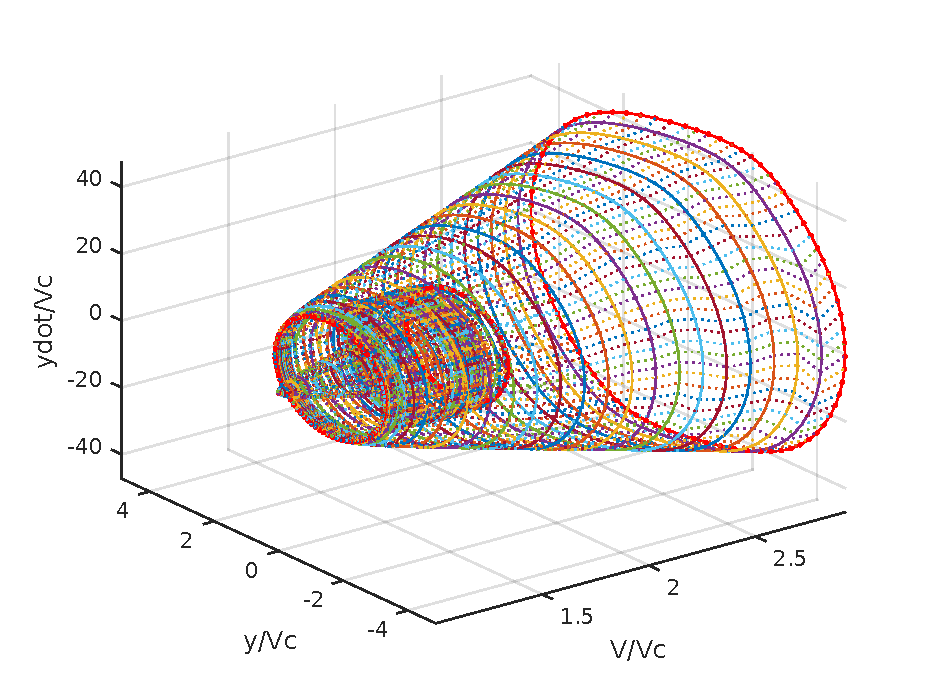
\includegraphics{./plots/matcont.pdf}
\caption{\texttt{matcont} output. The top plot an excerpt of the bottom 3D-graphic. The two additional bifurcation points $1.243$ and $1.823$ can be read off.}
\end{figure}




\end{document}